\documentclass[twoside]{book}

% Packages required by doxygen
\usepackage{fixltx2e}
\usepackage{calc}
\usepackage{doxygen}
\usepackage[export]{adjustbox} % also loads graphicx
\usepackage{graphicx}
\usepackage[utf8]{inputenc}
\usepackage{makeidx}
\usepackage{multicol}
\usepackage{multirow}
\PassOptionsToPackage{warn}{textcomp}
\usepackage{textcomp}
\usepackage[nointegrals]{wasysym}
\usepackage[table]{xcolor}

% Font selection
\usepackage[T1]{fontenc}
\usepackage[scaled=.90]{helvet}
\usepackage{courier}
\usepackage{amssymb}
\usepackage{sectsty}
\renewcommand{\familydefault}{\sfdefault}
\allsectionsfont{%
  \fontseries{bc}\selectfont%
  \color{darkgray}%
}
\renewcommand{\DoxyLabelFont}{%
  \fontseries{bc}\selectfont%
  \color{darkgray}%
}
\newcommand{\+}{\discretionary{\mbox{\scriptsize$\hookleftarrow$}}{}{}}

% Page & text layout
\usepackage{geometry}
\geometry{%
  a4paper,%
  top=2.5cm,%
  bottom=2.5cm,%
  left=2.5cm,%
  right=2.5cm%
}
\tolerance=750
\hfuzz=15pt
\hbadness=750
\setlength{\emergencystretch}{15pt}
\setlength{\parindent}{0cm}
\setlength{\parskip}{0.2cm}
\makeatletter
\renewcommand{\paragraph}{%
  \@startsection{paragraph}{4}{0ex}{-1.0ex}{1.0ex}{%
    \normalfont\normalsize\bfseries\SS@parafont%
  }%
}
\renewcommand{\subparagraph}{%
  \@startsection{subparagraph}{5}{0ex}{-1.0ex}{1.0ex}{%
    \normalfont\normalsize\bfseries\SS@subparafont%
  }%
}
\makeatother

% Headers & footers
\usepackage{fancyhdr}
\pagestyle{fancyplain}
\fancyhead[LE]{\fancyplain{}{\bfseries\thepage}}
\fancyhead[CE]{\fancyplain{}{}}
\fancyhead[RE]{\fancyplain{}{\bfseries\leftmark}}
\fancyhead[LO]{\fancyplain{}{\bfseries\rightmark}}
\fancyhead[CO]{\fancyplain{}{}}
\fancyhead[RO]{\fancyplain{}{\bfseries\thepage}}
\fancyfoot[LE]{\fancyplain{}{}}
\fancyfoot[CE]{\fancyplain{}{}}
\fancyfoot[RE]{\fancyplain{}{\bfseries\scriptsize Generated on Tue Apr 7 2015 19\+:39\+:18 for Simple\+Engine by Doxygen }}
\fancyfoot[LO]{\fancyplain{}{\bfseries\scriptsize Generated on Tue Apr 7 2015 19\+:39\+:18 for Simple\+Engine by Doxygen }}
\fancyfoot[CO]{\fancyplain{}{}}
\fancyfoot[RO]{\fancyplain{}{}}
\renewcommand{\footrulewidth}{0.4pt}
\renewcommand{\chaptermark}[1]{%
  \markboth{#1}{}%
}
\renewcommand{\sectionmark}[1]{%
  \markright{\thesection\ #1}%
}

% Indices & bibliography
\usepackage{natbib}
\usepackage[titles]{tocloft}
\setcounter{tocdepth}{3}
\setcounter{secnumdepth}{5}
\makeindex

% Custom commands
\newcommand{\clearemptydoublepage}{%
  \newpage{\pagestyle{empty}\cleardoublepage}%
}


%===== C O N T E N T S =====

\begin{document}

% Titlepage & ToC
\pagenumbering{roman}
\begin{titlepage}
\vspace*{7cm}
\begin{center}%
{\Large Simple\+Engine }\\
\vspace*{1cm}
{\large Generated by Doxygen 1.8.9.1}\\
\vspace*{0.5cm}
{\small Tue Apr 7 2015 19:39:18}\\
\end{center}
\end{titlepage}
\clearemptydoublepage
\tableofcontents
\clearemptydoublepage
\pagenumbering{arabic}

%--- Begin generated contents ---
\chapter{Namespace Index}
\section{Namespace List}
Here is a list of all namespaces with brief descriptions\+:\begin{DoxyCompactList}
\item\contentsline{section}{{\bf json} }{\pageref{namespacejson}}{}
\end{DoxyCompactList}

\chapter{Hierarchical Index}
\section{Class Hierarchy}
This inheritance list is sorted roughly, but not completely, alphabetically\+:\begin{DoxyCompactList}
\item \contentsline{section}{json\+:\+:Array}{\pageref{classjson_1_1_array}}{}
\item \contentsline{section}{json\+:\+:Object}{\pageref{classjson_1_1_object}}{}
\item \contentsline{section}{S\+E\+Application\+Interface}{\pageref{class_s_e_application_interface}}{}
\begin{DoxyCompactList}
\item \contentsline{section}{S\+E\+Application$<$ T $>$}{\pageref{class_s_e_application}}{}
\item \contentsline{section}{S\+E\+Application$<$ G\+Lfloat $>$}{\pageref{class_s_e_application}}{}
\begin{DoxyCompactList}
\item \contentsline{section}{S\+E\+Test\+App1}{\pageref{class_s_e_test_app1}}{}
\item \contentsline{section}{S\+E\+Test\+App2}{\pageref{class_s_e_test_app2}}{}
\end{DoxyCompactList}
\end{DoxyCompactList}
\item \contentsline{section}{S\+E\+Camera\+Type}{\pageref{struct_s_e_camera_type}}{}
\item \contentsline{section}{S\+E\+Chronometer$<$ T $>$}{\pageref{class_s_e_chronometer}}{}
\item \contentsline{section}{S\+E\+Configuration\+Loader\+:\+:S\+E\+Config\+Key}{\pageref{union_s_e_configuration_loader_1_1_s_e_config_key}}{}
\item \contentsline{section}{S\+E\+Configuration\+Loader}{\pageref{class_s_e_configuration_loader}}{}
\item \contentsline{section}{S\+E\+Event\+Handler}{\pageref{class_s_e_event_handler}}{}
\item \contentsline{section}{S\+E\+Flow\+Controller}{\pageref{class_s_e_flow_controller}}{}
\begin{DoxyCompactList}
\item \contentsline{section}{S\+E\+G\+L\+U\+T\+Flow\+Controller}{\pageref{class_s_e_g_l_u_t_flow_controller}}{}
\item \contentsline{section}{S\+E\+Null\+Flow\+Controller}{\pageref{class_s_e_null_flow_controller}}{}
\end{DoxyCompactList}
\item \contentsline{section}{S\+E\+Frustum\+Type}{\pageref{struct_s_e_frustum_type}}{}
\item \contentsline{section}{S\+E\+Light$<$ T $>$}{\pageref{class_s_e_light}}{}
\begin{DoxyCompactList}
\item \contentsline{section}{S\+E\+Ambient\+Light$<$ T $>$}{\pageref{class_s_e_ambient_light}}{}
\item \contentsline{section}{S\+E\+Directional\+Light$<$ T $>$}{\pageref{class_s_e_directional_light}}{}
\item \contentsline{section}{S\+E\+Point\+Light$<$ T $>$}{\pageref{class_s_e_point_light}}{}
\item \contentsline{section}{S\+E\+Spot\+Light$<$ T $>$}{\pageref{class_s_e_spot_light}}{}
\end{DoxyCompactList}
\item \contentsline{section}{S\+E\+Light$<$ G\+Lfloat $>$}{\pageref{class_s_e_light}}{}
\begin{DoxyCompactList}
\item \contentsline{section}{S\+E\+Ambient\+Light$<$ G\+Lfloat $>$}{\pageref{class_s_e_ambient_light}}{}
\begin{DoxyCompactList}
\item \contentsline{section}{S\+E\+Open\+G\+L\+Ambient\+Light}{\pageref{class_s_e_open_g_l_ambient_light}}{}
\end{DoxyCompactList}
\item \contentsline{section}{S\+E\+Directional\+Light$<$ G\+Lfloat $>$}{\pageref{class_s_e_directional_light}}{}
\begin{DoxyCompactList}
\item \contentsline{section}{S\+E\+Open\+G\+L\+Directional\+Light}{\pageref{class_s_e_open_g_l_directional_light}}{}
\end{DoxyCompactList}
\item \contentsline{section}{S\+E\+Open\+G\+L\+Light}{\pageref{class_s_e_open_g_l_light}}{}
\begin{DoxyCompactList}
\item \contentsline{section}{S\+E\+Open\+G\+L\+Ambient\+Light}{\pageref{class_s_e_open_g_l_ambient_light}}{}
\item \contentsline{section}{S\+E\+Open\+G\+L\+Directional\+Light}{\pageref{class_s_e_open_g_l_directional_light}}{}
\item \contentsline{section}{S\+E\+Open\+G\+L\+Point\+Light}{\pageref{class_s_e_open_g_l_point_light}}{}
\item \contentsline{section}{S\+E\+Open\+G\+L\+Spot\+Light}{\pageref{class_s_e_open_g_l_spot_light}}{}
\end{DoxyCompactList}
\item \contentsline{section}{S\+E\+Point\+Light$<$ G\+Lfloat $>$}{\pageref{class_s_e_point_light}}{}
\begin{DoxyCompactList}
\item \contentsline{section}{S\+E\+Open\+G\+L\+Point\+Light}{\pageref{class_s_e_open_g_l_point_light}}{}
\end{DoxyCompactList}
\item \contentsline{section}{S\+E\+Spot\+Light$<$ G\+Lfloat $>$}{\pageref{class_s_e_spot_light}}{}
\begin{DoxyCompactList}
\item \contentsline{section}{S\+E\+Open\+G\+L\+Spot\+Light}{\pageref{class_s_e_open_g_l_spot_light}}{}
\end{DoxyCompactList}
\end{DoxyCompactList}
\item \contentsline{section}{S\+E\+Light\+Types}{\pageref{struct_s_e_light_types}}{}
\item \contentsline{section}{S\+E\+Mat3$<$ T $>$}{\pageref{class_s_e_mat3}}{}
\item \contentsline{section}{S\+E\+Mat4$<$ T $>$}{\pageref{class_s_e_mat4}}{}
\item \contentsline{section}{S\+E\+Mat4$<$ G\+Lfloat $>$}{\pageref{class_s_e_mat4}}{}
\item \contentsline{section}{S\+E\+Math\+Util$<$ T $>$}{\pageref{class_s_e_math_util}}{}
\item \contentsline{section}{S\+E\+Object}{\pageref{class_s_e_object}}{}
\begin{DoxyCompactList}
\item \contentsline{section}{S\+E\+Component}{\pageref{class_s_e_component}}{}
\begin{DoxyCompactList}
\item \contentsline{section}{S\+E\+Render\+Component}{\pageref{class_s_e_render_component}}{}
\end{DoxyCompactList}
\item \contentsline{section}{S\+E\+Entity}{\pageref{class_s_e_entity}}{}
\end{DoxyCompactList}
\item \contentsline{section}{S\+E\+Object\+Name}{\pageref{class_s_e_object_name}}{}
\item \contentsline{section}{S\+E\+Plane$<$ T $>$}{\pageref{class_s_e_plane}}{}
\item \contentsline{section}{S\+E\+Primitive$<$ T $>$}{\pageref{class_s_e_primitive}}{}
\begin{DoxyCompactList}
\item \contentsline{section}{S\+E\+Cone$<$ T $>$}{\pageref{class_s_e_cone}}{}
\item \contentsline{section}{S\+E\+Cube$<$ T $>$}{\pageref{class_s_e_cube}}{}
\item \contentsline{section}{S\+E\+Sphere$<$ T $>$}{\pageref{class_s_e_sphere}}{}
\item \contentsline{section}{S\+E\+Teapot$<$ T $>$}{\pageref{class_s_e_teapot}}{}
\item \contentsline{section}{S\+E\+Torus$<$ T $>$}{\pageref{class_s_e_torus}}{}
\end{DoxyCompactList}
\item \contentsline{section}{S\+E\+Primitive$<$ G\+Lfloat $>$}{\pageref{class_s_e_primitive}}{}
\begin{DoxyCompactList}
\item \contentsline{section}{S\+E\+Cone$<$ G\+Lfloat $>$}{\pageref{class_s_e_cone}}{}
\begin{DoxyCompactList}
\item \contentsline{section}{S\+E\+Open\+G\+L\+Cone}{\pageref{class_s_e_open_g_l_cone}}{}
\end{DoxyCompactList}
\item \contentsline{section}{S\+E\+Cube$<$ G\+Lfloat $>$}{\pageref{class_s_e_cube}}{}
\begin{DoxyCompactList}
\item \contentsline{section}{S\+E\+Open\+G\+L\+Cube}{\pageref{class_s_e_open_g_l_cube}}{}
\end{DoxyCompactList}
\item \contentsline{section}{S\+E\+Open\+G\+L\+Primitive}{\pageref{class_s_e_open_g_l_primitive}}{}
\begin{DoxyCompactList}
\item \contentsline{section}{S\+E\+Open\+G\+L\+Cone}{\pageref{class_s_e_open_g_l_cone}}{}
\item \contentsline{section}{S\+E\+Open\+G\+L\+Cube}{\pageref{class_s_e_open_g_l_cube}}{}
\item \contentsline{section}{S\+E\+Open\+G\+L\+Sphere}{\pageref{class_s_e_open_g_l_sphere}}{}
\item \contentsline{section}{S\+E\+Open\+G\+L\+Teapot}{\pageref{class_s_e_open_g_l_teapot}}{}
\item \contentsline{section}{S\+E\+Open\+G\+L\+Torus}{\pageref{class_s_e_open_g_l_torus}}{}
\end{DoxyCompactList}
\item \contentsline{section}{S\+E\+Sphere$<$ G\+Lfloat $>$}{\pageref{class_s_e_sphere}}{}
\begin{DoxyCompactList}
\item \contentsline{section}{S\+E\+Open\+G\+L\+Sphere}{\pageref{class_s_e_open_g_l_sphere}}{}
\end{DoxyCompactList}
\item \contentsline{section}{S\+E\+Teapot$<$ G\+Lfloat $>$}{\pageref{class_s_e_teapot}}{}
\begin{DoxyCompactList}
\item \contentsline{section}{S\+E\+Open\+G\+L\+Teapot}{\pageref{class_s_e_open_g_l_teapot}}{}
\end{DoxyCompactList}
\item \contentsline{section}{S\+E\+Torus$<$ G\+Lfloat $>$}{\pageref{class_s_e_torus}}{}
\begin{DoxyCompactList}
\item \contentsline{section}{S\+E\+Open\+G\+L\+Torus}{\pageref{class_s_e_open_g_l_torus}}{}
\end{DoxyCompactList}
\end{DoxyCompactList}
\item \contentsline{section}{S\+E\+Prim\+Types}{\pageref{struct_s_e_prim_types}}{}
\item \contentsline{section}{S\+E\+Quaternion$<$ T $>$}{\pageref{class_s_e_quaternion}}{}
\item \contentsline{section}{S\+E\+Quaternion$<$ G\+Lfloat $>$}{\pageref{class_s_e_quaternion}}{}
\item \contentsline{section}{S\+E\+Random\+Number\+Generator$<$ T $>$}{\pageref{class_s_e_random_number_generator}}{}
\item \contentsline{section}{S\+E\+Ray$<$ T $>$}{\pageref{class_s_e_ray}}{}
\item \contentsline{section}{S\+E\+Render\+Object$<$ T $>$}{\pageref{class_s_e_render_object}}{}
\begin{DoxyCompactList}
\item \contentsline{section}{S\+E\+Camera$<$ T $>$}{\pageref{class_s_e_camera}}{}
\item \contentsline{section}{S\+E\+Cone$<$ T $>$}{\pageref{class_s_e_cone}}{}
\item \contentsline{section}{S\+E\+Cube$<$ T $>$}{\pageref{class_s_e_cube}}{}
\item \contentsline{section}{S\+E\+Mesh$<$ T $>$}{\pageref{class_s_e_mesh}}{}
\begin{DoxyCompactList}
\item \contentsline{section}{S\+E\+M\+D2\+Mesh$<$ T $>$}{\pageref{class_s_e_m_d2_mesh}}{}
\end{DoxyCompactList}
\item \contentsline{section}{S\+E\+Model$<$ T $>$}{\pageref{class_s_e_model}}{}
\item \contentsline{section}{S\+E\+Sphere$<$ T $>$}{\pageref{class_s_e_sphere}}{}
\item \contentsline{section}{S\+E\+Teapot$<$ T $>$}{\pageref{class_s_e_teapot}}{}
\item \contentsline{section}{S\+E\+Torus$<$ T $>$}{\pageref{class_s_e_torus}}{}
\end{DoxyCompactList}
\item \contentsline{section}{S\+E\+Render\+Object$<$ G\+Lfloat $>$}{\pageref{class_s_e_render_object}}{}
\begin{DoxyCompactList}
\item \contentsline{section}{S\+E\+Camera$<$ G\+Lfloat $>$}{\pageref{class_s_e_camera}}{}
\begin{DoxyCompactList}
\item \contentsline{section}{S\+E\+Open\+G\+L\+Camera}{\pageref{class_s_e_open_g_l_camera}}{}
\end{DoxyCompactList}
\item \contentsline{section}{S\+E\+Cone$<$ G\+Lfloat $>$}{\pageref{class_s_e_cone}}{}
\item \contentsline{section}{S\+E\+Cube$<$ G\+Lfloat $>$}{\pageref{class_s_e_cube}}{}
\item \contentsline{section}{S\+E\+Open\+G\+L\+Render\+Object}{\pageref{class_s_e_open_g_l_render_object}}{}
\begin{DoxyCompactList}
\item \contentsline{section}{S\+E\+Open\+G\+L\+Camera}{\pageref{class_s_e_open_g_l_camera}}{}
\item \contentsline{section}{S\+E\+Open\+G\+L\+Light}{\pageref{class_s_e_open_g_l_light}}{}
\item \contentsline{section}{S\+E\+Open\+G\+L\+Primitive}{\pageref{class_s_e_open_g_l_primitive}}{}
\end{DoxyCompactList}
\item \contentsline{section}{S\+E\+Sphere$<$ G\+Lfloat $>$}{\pageref{class_s_e_sphere}}{}
\item \contentsline{section}{S\+E\+Teapot$<$ G\+Lfloat $>$}{\pageref{class_s_e_teapot}}{}
\item \contentsline{section}{S\+E\+Torus$<$ G\+Lfloat $>$}{\pageref{class_s_e_torus}}{}
\end{DoxyCompactList}
\item \contentsline{section}{S\+E\+Render\+Service}{\pageref{class_s_e_render_service}}{}
\begin{DoxyCompactList}
\item \contentsline{section}{S\+E\+Render\+Service\+Internals$<$ T $>$}{\pageref{class_s_e_render_service_internals}}{}
\item \contentsline{section}{S\+E\+Render\+Service\+Internals$<$ G\+Lfloat $>$}{\pageref{class_s_e_render_service_internals}}{}
\begin{DoxyCompactList}
\item \contentsline{section}{S\+E\+Open\+G\+L\+Render\+Service}{\pageref{class_s_e_open_g_l_render_service}}{}
\end{DoxyCompactList}
\item \contentsline{section}{S\+E\+Render\+Service\+Internals$<$ int $>$}{\pageref{class_s_e_render_service_internals}}{}
\begin{DoxyCompactList}
\item \contentsline{section}{S\+E\+Null\+Render\+Service}{\pageref{class_s_e_null_render_service}}{}
\end{DoxyCompactList}
\end{DoxyCompactList}
\item \contentsline{section}{S\+E\+R\+O\+Type}{\pageref{struct_s_e_r_o_type}}{}
\item \contentsline{section}{S\+E\+Scene}{\pageref{class_s_e_scene}}{}
\item \contentsline{section}{S\+E\+Scene\+Graph}{\pageref{class_s_e_scene_graph}}{}
\item \contentsline{section}{S\+E\+Scene\+Manager}{\pageref{class_s_e_scene_manager}}{}
\item \contentsline{section}{S\+E\+Service\+Locator}{\pageref{class_s_e_service_locator}}{}
\item \contentsline{section}{S\+E\+Skeleton$<$ T $>$}{\pageref{class_s_e_skeleton}}{}
\item \contentsline{section}{S\+E\+Timer$<$ T $>$}{\pageref{class_s_e_timer}}{}
\item \contentsline{section}{S\+E\+Timer$<$ double $>$}{\pageref{class_s_e_timer}}{}
\item \contentsline{section}{S\+E\+Timer$<$ G\+Lfloat $>$}{\pageref{class_s_e_timer}}{}
\item \contentsline{section}{S\+E\+Vec3$<$ T $>$}{\pageref{class_s_e_vec3}}{}
\item \contentsline{section}{S\+E\+Vec3$<$ G\+Lfloat $>$}{\pageref{class_s_e_vec3}}{}
\item \contentsline{section}{S\+E\+Vec4$<$ T $>$}{\pageref{class_s_e_vec4}}{}
\begin{DoxyCompactList}
\item \contentsline{section}{S\+E\+Color$<$ T $>$}{\pageref{class_s_e_color}}{}
\end{DoxyCompactList}
\item \contentsline{section}{S\+E\+Vec4$<$ G\+Lfloat $>$}{\pageref{class_s_e_vec4}}{}
\begin{DoxyCompactList}
\item \contentsline{section}{S\+E\+Color$<$ G\+Lfloat $>$}{\pageref{class_s_e_color}}{}
\end{DoxyCompactList}
\item \contentsline{section}{S\+E\+Vertex$<$ T $>$}{\pageref{class_s_e_vertex}}{}
\item \contentsline{section}{S\+E\+Vertex\+Buffer$<$ T $>$}{\pageref{class_s_e_vertex_buffer}}{}
\item \contentsline{section}{S\+E\+Window}{\pageref{class_s_e_window}}{}
\begin{DoxyCompactList}
\item \contentsline{section}{S\+E\+G\+L\+U\+I\+Window}{\pageref{class_s_e_g_l_u_i_window}}{}
\item \contentsline{section}{S\+E\+Null\+Window}{\pageref{class_s_e_null_window}}{}
\end{DoxyCompactList}
\item \contentsline{section}{S\+E\+Window\+Manager}{\pageref{class_s_e_window_manager}}{}
\begin{DoxyCompactList}
\item \contentsline{section}{S\+E\+G\+L\+U\+I\+Window\+Manager}{\pageref{class_s_e_g_l_u_i_window_manager}}{}
\item \contentsline{section}{S\+E\+Null\+Window\+Manager}{\pageref{class_s_e_null_window_manager}}{}
\end{DoxyCompactList}
\item \contentsline{section}{Simple\+Engine}{\pageref{class_simple_engine}}{}
\item \contentsline{section}{t\+M\+D2}{\pageref{structt_m_d2}}{}
\item \contentsline{section}{t\+M\+D2\+Frame$<$ T $>$}{\pageref{structt_m_d2_frame}}{}
\item \contentsline{section}{t\+M\+D2\+Vertex}{\pageref{structt_m_d2_vertex}}{}
\item \contentsline{section}{json\+:\+:Value}{\pageref{classjson_1_1_value}}{}
\end{DoxyCompactList}

\chapter{Class Index}
\section{Class List}
Here are the classes, structs, unions and interfaces with brief descriptions\+:\begin{DoxyCompactList}
\item\contentsline{section}{{\bf json\+::\+Array} }{\pageref{classjson_1_1_array}}{}
\item\contentsline{section}{{\bf json\+::\+Object} }{\pageref{classjson_1_1_object}}{}
\item\contentsline{section}{{\bf S\+E\+Ambient\+Light$<$ T $>$} }{\pageref{class_s_e_ambient_light}}{}
\item\contentsline{section}{{\bf S\+E\+Application$<$ T $>$} }{\pageref{class_s_e_application}}{}
\item\contentsline{section}{{\bf S\+E\+Application\+Interface} }{\pageref{class_s_e_application_interface}}{}
\item\contentsline{section}{{\bf S\+E\+Camera$<$ T $>$} }{\pageref{class_s_e_camera}}{}
\item\contentsline{section}{{\bf S\+E\+Camera\+Type} }{\pageref{struct_s_e_camera_type}}{}
\item\contentsline{section}{{\bf S\+E\+Chronometer$<$ T $>$} }{\pageref{class_s_e_chronometer}}{}
\item\contentsline{section}{{\bf S\+E\+Color$<$ T $>$} }{\pageref{class_s_e_color}}{}
\item\contentsline{section}{{\bf S\+E\+Component} }{\pageref{class_s_e_component}}{}
\item\contentsline{section}{{\bf S\+E\+Cone$<$ T $>$} }{\pageref{class_s_e_cone}}{}
\item\contentsline{section}{{\bf S\+E\+Configuration\+Loader\+::\+S\+E\+Config\+Key} }{\pageref{union_s_e_configuration_loader_1_1_s_e_config_key}}{}
\item\contentsline{section}{{\bf S\+E\+Configuration\+Loader} }{\pageref{class_s_e_configuration_loader}}{}
\item\contentsline{section}{{\bf S\+E\+Cube$<$ T $>$} }{\pageref{class_s_e_cube}}{}
\item\contentsline{section}{{\bf S\+E\+Directional\+Light$<$ T $>$} }{\pageref{class_s_e_directional_light}}{}
\item\contentsline{section}{{\bf S\+E\+Entity} }{\pageref{class_s_e_entity}}{}
\item\contentsline{section}{{\bf S\+E\+Event\+Handler} }{\pageref{class_s_e_event_handler}}{}
\item\contentsline{section}{{\bf S\+E\+Flow\+Controller} }{\pageref{class_s_e_flow_controller}}{}
\item\contentsline{section}{{\bf S\+E\+Frustum\+Type} }{\pageref{struct_s_e_frustum_type}}{}
\item\contentsline{section}{{\bf S\+E\+G\+L\+U\+I\+Window} }{\pageref{class_s_e_g_l_u_i_window}}{}
\item\contentsline{section}{{\bf S\+E\+G\+L\+U\+I\+Window\+Manager} }{\pageref{class_s_e_g_l_u_i_window_manager}}{}
\item\contentsline{section}{{\bf S\+E\+G\+L\+U\+T\+Flow\+Controller} }{\pageref{class_s_e_g_l_u_t_flow_controller}}{}
\item\contentsline{section}{{\bf S\+E\+Light$<$ T $>$} }{\pageref{class_s_e_light}}{}
\item\contentsline{section}{{\bf S\+E\+Light\+Types} }{\pageref{struct_s_e_light_types}}{}
\item\contentsline{section}{{\bf S\+E\+Mat3$<$ T $>$} }{\pageref{class_s_e_mat3}}{}
\item\contentsline{section}{{\bf S\+E\+Mat4$<$ T $>$} }{\pageref{class_s_e_mat4}}{}
\item\contentsline{section}{{\bf S\+E\+Math\+Util$<$ T $>$} }{\pageref{class_s_e_math_util}}{}
\item\contentsline{section}{{\bf S\+E\+M\+D2\+Mesh$<$ T $>$} }{\pageref{class_s_e_m_d2_mesh}}{}
\item\contentsline{section}{{\bf S\+E\+Mesh$<$ T $>$} }{\pageref{class_s_e_mesh}}{}
\item\contentsline{section}{{\bf S\+E\+Model$<$ T $>$} }{\pageref{class_s_e_model}}{}
\item\contentsline{section}{{\bf S\+E\+Null\+Flow\+Controller} }{\pageref{class_s_e_null_flow_controller}}{}
\item\contentsline{section}{{\bf S\+E\+Null\+Render\+Service} }{\pageref{class_s_e_null_render_service}}{}
\item\contentsline{section}{{\bf S\+E\+Null\+Window} }{\pageref{class_s_e_null_window}}{}
\item\contentsline{section}{{\bf S\+E\+Null\+Window\+Manager} }{\pageref{class_s_e_null_window_manager}}{}
\item\contentsline{section}{{\bf S\+E\+Object} }{\pageref{class_s_e_object}}{}
\item\contentsline{section}{{\bf S\+E\+Object\+Name} }{\pageref{class_s_e_object_name}}{}
\item\contentsline{section}{{\bf S\+E\+Open\+G\+L\+Ambient\+Light} }{\pageref{class_s_e_open_g_l_ambient_light}}{}
\item\contentsline{section}{{\bf S\+E\+Open\+G\+L\+Camera} }{\pageref{class_s_e_open_g_l_camera}}{}
\item\contentsline{section}{{\bf S\+E\+Open\+G\+L\+Cone} }{\pageref{class_s_e_open_g_l_cone}}{}
\item\contentsline{section}{{\bf S\+E\+Open\+G\+L\+Cube} }{\pageref{class_s_e_open_g_l_cube}}{}
\item\contentsline{section}{{\bf S\+E\+Open\+G\+L\+Directional\+Light} }{\pageref{class_s_e_open_g_l_directional_light}}{}
\item\contentsline{section}{{\bf S\+E\+Open\+G\+L\+Light} }{\pageref{class_s_e_open_g_l_light}}{}
\item\contentsline{section}{{\bf S\+E\+Open\+G\+L\+Point\+Light} }{\pageref{class_s_e_open_g_l_point_light}}{}
\item\contentsline{section}{{\bf S\+E\+Open\+G\+L\+Primitive} }{\pageref{class_s_e_open_g_l_primitive}}{}
\item\contentsline{section}{{\bf S\+E\+Open\+G\+L\+Render\+Object} }{\pageref{class_s_e_open_g_l_render_object}}{}
\item\contentsline{section}{{\bf S\+E\+Open\+G\+L\+Render\+Service} }{\pageref{class_s_e_open_g_l_render_service}}{}
\item\contentsline{section}{{\bf S\+E\+Open\+G\+L\+Sphere} }{\pageref{class_s_e_open_g_l_sphere}}{}
\item\contentsline{section}{{\bf S\+E\+Open\+G\+L\+Spot\+Light} }{\pageref{class_s_e_open_g_l_spot_light}}{}
\item\contentsline{section}{{\bf S\+E\+Open\+G\+L\+Teapot} }{\pageref{class_s_e_open_g_l_teapot}}{}
\item\contentsline{section}{{\bf S\+E\+Open\+G\+L\+Torus} }{\pageref{class_s_e_open_g_l_torus}}{}
\item\contentsline{section}{{\bf S\+E\+Plane$<$ T $>$} }{\pageref{class_s_e_plane}}{}
\item\contentsline{section}{{\bf S\+E\+Point\+Light$<$ T $>$} }{\pageref{class_s_e_point_light}}{}
\item\contentsline{section}{{\bf S\+E\+Primitive$<$ T $>$} }{\pageref{class_s_e_primitive}}{}
\item\contentsline{section}{{\bf S\+E\+Prim\+Types} }{\pageref{struct_s_e_prim_types}}{}
\item\contentsline{section}{{\bf S\+E\+Quaternion$<$ T $>$} }{\pageref{class_s_e_quaternion}}{}
\item\contentsline{section}{{\bf S\+E\+Random\+Number\+Generator$<$ T $>$} }{\pageref{class_s_e_random_number_generator}}{}
\item\contentsline{section}{{\bf S\+E\+Ray$<$ T $>$} }{\pageref{class_s_e_ray}}{}
\item\contentsline{section}{{\bf S\+E\+Render\+Component} }{\pageref{class_s_e_render_component}}{}
\item\contentsline{section}{{\bf S\+E\+Render\+Object$<$ T $>$} }{\pageref{class_s_e_render_object}}{}
\item\contentsline{section}{{\bf S\+E\+Render\+Service} }{\pageref{class_s_e_render_service}}{}
\item\contentsline{section}{{\bf S\+E\+Render\+Service\+Internals$<$ T $>$} }{\pageref{class_s_e_render_service_internals}}{}
\item\contentsline{section}{{\bf S\+E\+R\+O\+Type} }{\pageref{struct_s_e_r_o_type}}{}
\item\contentsline{section}{{\bf S\+E\+Scene} }{\pageref{class_s_e_scene}}{}
\item\contentsline{section}{{\bf S\+E\+Scene\+Graph} }{\pageref{class_s_e_scene_graph}}{}
\item\contentsline{section}{{\bf S\+E\+Scene\+Manager} }{\pageref{class_s_e_scene_manager}}{}
\item\contentsline{section}{{\bf S\+E\+Service\+Locator} }{\pageref{class_s_e_service_locator}}{}
\item\contentsline{section}{{\bf S\+E\+Skeleton$<$ T $>$} }{\pageref{class_s_e_skeleton}}{}
\item\contentsline{section}{{\bf S\+E\+Sphere$<$ T $>$} }{\pageref{class_s_e_sphere}}{}
\item\contentsline{section}{{\bf S\+E\+Spot\+Light$<$ T $>$} }{\pageref{class_s_e_spot_light}}{}
\item\contentsline{section}{{\bf S\+E\+Teapot$<$ T $>$} }{\pageref{class_s_e_teapot}}{}
\item\contentsline{section}{{\bf S\+E\+Test\+App1} }{\pageref{class_s_e_test_app1}}{}
\item\contentsline{section}{{\bf S\+E\+Test\+App2} }{\pageref{class_s_e_test_app2}}{}
\item\contentsline{section}{{\bf S\+E\+Timer$<$ T $>$} }{\pageref{class_s_e_timer}}{}
\item\contentsline{section}{{\bf S\+E\+Torus$<$ T $>$} }{\pageref{class_s_e_torus}}{}
\item\contentsline{section}{{\bf S\+E\+Vec3$<$ T $>$} }{\pageref{class_s_e_vec3}}{}
\item\contentsline{section}{{\bf S\+E\+Vec4$<$ T $>$} }{\pageref{class_s_e_vec4}}{}
\item\contentsline{section}{{\bf S\+E\+Vertex$<$ T $>$} }{\pageref{class_s_e_vertex}}{}
\item\contentsline{section}{{\bf S\+E\+Vertex\+Buffer$<$ T $>$} }{\pageref{class_s_e_vertex_buffer}}{}
\item\contentsline{section}{{\bf S\+E\+Window} }{\pageref{class_s_e_window}}{}
\item\contentsline{section}{{\bf S\+E\+Window\+Manager} }{\pageref{class_s_e_window_manager}}{}
\item\contentsline{section}{{\bf Simple\+Engine} }{\pageref{class_simple_engine}}{}
\item\contentsline{section}{{\bf t\+M\+D2} }{\pageref{structt_m_d2}}{}
\item\contentsline{section}{{\bf t\+M\+D2\+Frame$<$ T $>$} }{\pageref{structt_m_d2_frame}}{}
\item\contentsline{section}{{\bf t\+M\+D2\+Vertex} }{\pageref{structt_m_d2_vertex}}{}
\item\contentsline{section}{{\bf json\+::\+Value} }{\pageref{classjson_1_1_value}}{}
\end{DoxyCompactList}

\chapter{File Index}
\section{File List}
Here is a list of all files with brief descriptions\+:\begin{DoxyCompactList}
\item\contentsline{section}{{\bf json.\+cpp} }{\pageref{json_8cpp}}{}
\item\contentsline{section}{{\bf json.\+h} }{\pageref{json_8h}}{}
\item\contentsline{section}{{\bf S\+E\+Test\+App1/main.\+cpp} }{\pageref{_s_e_test_app1_2main_8cpp}}{}
\item\contentsline{section}{{\bf S\+E\+Test\+App2/main.\+cpp} }{\pageref{_s_e_test_app2_2main_8cpp}}{}
\item\contentsline{section}{{\bf src/main.\+cpp} }{\pageref{src_2main_8cpp}}{}
\item\contentsline{section}{{\bf M\+D2\+Normals.\+h} }{\pageref{_m_d2_normals_8h}}{}
\item\contentsline{section}{{\bf M\+D2\+Normals\+Tab.\+h} }{\pageref{_m_d2_normals_tab_8h}}{}
\item\contentsline{section}{{\bf S\+E\+Application.\+cpp} }{\pageref{_s_e_application_8cpp}}{}
\item\contentsline{section}{{\bf S\+E\+Application.\+h} }{\pageref{_s_e_application_8h}}{}
\item\contentsline{section}{{\bf S\+E\+Application\+Interface.\+h} }{\pageref{_s_e_application_interface_8h}}{}
\item\contentsline{section}{{\bf S\+E\+Camera.\+h} }{\pageref{_s_e_camera_8h}}{}
\item\contentsline{section}{{\bf S\+E\+Component.\+h} }{\pageref{_s_e_component_8h}}{}
\item\contentsline{section}{{\bf S\+E\+Configuration\+Loader.\+cpp} }{\pageref{_s_e_configuration_loader_8cpp}}{}
\item\contentsline{section}{{\bf S\+E\+Configuration\+Loader.\+h} }{\pageref{_s_e_configuration_loader_8h}}{}
\item\contentsline{section}{{\bf S\+E\+Debug\+Tools.\+cpp} }{\pageref{_s_e_debug_tools_8cpp}}{}
\item\contentsline{section}{{\bf S\+E\+Debug\+Tools.\+h} }{\pageref{_s_e_debug_tools_8h}}{}
\item\contentsline{section}{{\bf S\+E\+Entity.\+h} }{\pageref{_s_e_entity_8h}}{}
\item\contentsline{section}{{\bf S\+E\+Event\+Handler.\+h} }{\pageref{_s_e_event_handler_8h}}{}
\item\contentsline{section}{{\bf S\+E\+Flow\+Controller.\+h} }{\pageref{_s_e_flow_controller_8h}}{}
\item\contentsline{section}{{\bf S\+E\+G\+L\+U\+I\+Window.\+cpp} }{\pageref{_s_e_g_l_u_i_window_8cpp}}{}
\item\contentsline{section}{{\bf S\+E\+G\+L\+U\+I\+Window.\+h} }{\pageref{_s_e_g_l_u_i_window_8h}}{}
\item\contentsline{section}{{\bf S\+E\+G\+L\+U\+I\+Window\+Manager.\+cpp} }{\pageref{_s_e_g_l_u_i_window_manager_8cpp}}{}
\item\contentsline{section}{{\bf S\+E\+G\+L\+U\+I\+Window\+Manager.\+h} }{\pageref{_s_e_g_l_u_i_window_manager_8h}}{}
\item\contentsline{section}{{\bf S\+E\+G\+L\+U\+T\+Flow\+Controller.\+cpp} }{\pageref{_s_e_g_l_u_t_flow_controller_8cpp}}{}
\item\contentsline{section}{{\bf S\+E\+G\+L\+U\+T\+Flow\+Controller.\+h} }{\pageref{_s_e_g_l_u_t_flow_controller_8h}}{}
\item\contentsline{section}{{\bf S\+E\+Light.\+h} }{\pageref{_s_e_light_8h}}{}
\item\contentsline{section}{{\bf S\+E\+Material.\+h} }{\pageref{_s_e_material_8h}}{}
\item\contentsline{section}{{\bf S\+E\+Math.\+cpp} }{\pageref{_s_e_math_8cpp}}{}
\item\contentsline{section}{{\bf S\+E\+Math.\+h} }{\pageref{_s_e_math_8h}}{}
\item\contentsline{section}{{\bf S\+E\+M\+D2\+Mesh.\+cpp} }{\pageref{_s_e_m_d2_mesh_8cpp}}{}
\item\contentsline{section}{{\bf S\+E\+M\+D2\+Mesh.\+h} }{\pageref{_s_e_m_d2_mesh_8h}}{}
\item\contentsline{section}{{\bf S\+E\+Mesh.\+cpp} }{\pageref{_s_e_mesh_8cpp}}{}
\item\contentsline{section}{{\bf S\+E\+Mesh.\+h} }{\pageref{_s_e_mesh_8h}}{}
\item\contentsline{section}{{\bf S\+E\+Model.\+cpp} }{\pageref{_s_e_model_8cpp}}{}
\item\contentsline{section}{{\bf S\+E\+Model.\+h} }{\pageref{_s_e_model_8h}}{}
\item\contentsline{section}{{\bf S\+E\+Object.\+cpp} }{\pageref{_s_e_object_8cpp}}{}
\item\contentsline{section}{{\bf S\+E\+Object.\+h} }{\pageref{_s_e_object_8h}}{}
\item\contentsline{section}{{\bf S\+E\+Open\+G\+L\+Camera.\+cpp} }{\pageref{_s_e_open_g_l_camera_8cpp}}{}
\item\contentsline{section}{{\bf S\+E\+Open\+G\+L\+Camera.\+h} }{\pageref{_s_e_open_g_l_camera_8h}}{}
\item\contentsline{section}{{\bf S\+E\+Open\+G\+L\+Light.\+cpp} }{\pageref{_s_e_open_g_l_light_8cpp}}{}
\item\contentsline{section}{{\bf S\+E\+Open\+G\+L\+Light.\+h} }{\pageref{_s_e_open_g_l_light_8h}}{}
\item\contentsline{section}{{\bf S\+E\+Open\+G\+L\+Primitive.\+cpp} }{\pageref{_s_e_open_g_l_primitive_8cpp}}{}
\item\contentsline{section}{{\bf S\+E\+Open\+G\+L\+Primitive.\+h} }{\pageref{_s_e_open_g_l_primitive_8h}}{}
\item\contentsline{section}{{\bf S\+E\+Open\+G\+L\+Render\+Object.\+cpp} }{\pageref{_s_e_open_g_l_render_object_8cpp}}{}
\item\contentsline{section}{{\bf S\+E\+Open\+G\+L\+Render\+Object.\+h} }{\pageref{_s_e_open_g_l_render_object_8h}}{}
\item\contentsline{section}{{\bf S\+E\+Open\+G\+L\+Render\+Service.\+cpp} }{\pageref{_s_e_open_g_l_render_service_8cpp}}{}
\item\contentsline{section}{{\bf S\+E\+Open\+G\+L\+Render\+Service.\+h} }{\pageref{_s_e_open_g_l_render_service_8h}}{}
\item\contentsline{section}{{\bf S\+E\+Primitive.\+h} }{\pageref{_s_e_primitive_8h}}{}
\item\contentsline{section}{{\bf S\+E\+Render\+Component.\+h} }{\pageref{_s_e_render_component_8h}}{}
\item\contentsline{section}{{\bf S\+E\+Render\+Object.\+h} }{\pageref{_s_e_render_object_8h}}{}
\item\contentsline{section}{{\bf S\+E\+Render\+Service.\+cpp} }{\pageref{_s_e_render_service_8cpp}}{}
\item\contentsline{section}{{\bf S\+E\+Render\+Service.\+h} }{\pageref{_s_e_render_service_8h}}{}
\item\contentsline{section}{{\bf S\+E\+R\+O\+Builder.\+h} }{\pageref{_s_e_r_o_builder_8h}}{}
\item\contentsline{section}{{\bf S\+E\+Scene.\+h} }{\pageref{_s_e_scene_8h}}{}
\item\contentsline{section}{{\bf S\+E\+Scene\+Graph.\+h} }{\pageref{_s_e_scene_graph_8h}}{}
\item\contentsline{section}{{\bf S\+E\+Scene\+Manager.\+h} }{\pageref{_s_e_scene_manager_8h}}{}
\item\contentsline{section}{{\bf S\+E\+Service\+Locator.\+cpp} }{\pageref{_s_e_service_locator_8cpp}}{}
\item\contentsline{section}{{\bf S\+E\+Service\+Locator.\+h} }{\pageref{_s_e_service_locator_8h}}{}
\item\contentsline{section}{{\bf S\+E\+Test\+App1.\+cpp} }{\pageref{_s_e_test_app1_8cpp}}{}
\item\contentsline{section}{{\bf S\+E\+Test\+App1.\+hpp} }{\pageref{_s_e_test_app1_8hpp}}{}
\item\contentsline{section}{{\bf S\+E\+Test\+App2.\+cpp} }{\pageref{_s_e_test_app2_8cpp}}{}
\item\contentsline{section}{{\bf S\+E\+Test\+App2.\+hpp} }{\pageref{_s_e_test_app2_8hpp}}{}
\item\contentsline{section}{{\bf S\+E\+Vertex.\+h} }{\pageref{_s_e_vertex_8h}}{}
\item\contentsline{section}{{\bf S\+E\+Vertex\+Buffer.\+h} }{\pageref{_s_e_vertex_buffer_8h}}{}
\item\contentsline{section}{{\bf S\+E\+Window.\+h} }{\pageref{_s_e_window_8h}}{}
\item\contentsline{section}{{\bf S\+E\+Window\+Manager.\+h} }{\pageref{_s_e_window_manager_8h}}{}
\item\contentsline{section}{{\bf Simple\+Engine.\+cpp} }{\pageref{_simple_engine_8cpp}}{}
\item\contentsline{section}{{\bf Simple\+Engine.\+h} }{\pageref{_simple_engine_8h}}{}
\end{DoxyCompactList}

\chapter{Namespace Documentation}
\section{json Namespace Reference}
\label{namespacejson}\index{json@{json}}
\subsection*{Classes}
\begin{DoxyCompactItemize}
\item 
class {\bf Array}
\item 
class {\bf Object}
\item 
class {\bf Value}
\end{DoxyCompactItemize}
\subsection*{Enumerations}
\begin{DoxyCompactItemize}
\item 
enum {\bf Value\+Type} \{ \\*
{\bf N\+U\+L\+L\+Val}, 
{\bf String\+Val}, 
{\bf Int\+Val}, 
{\bf Float\+Val}, 
\\*
{\bf Double\+Val}, 
{\bf Object\+Val}, 
{\bf Array\+Val}, 
{\bf Bool\+Val}
 \}
\item 
enum {\bf Stack\+Depth\+Type} \{ {\bf In\+Object}, 
{\bf In\+Array}
 \}
\end{DoxyCompactItemize}
\subsection*{Functions}
\begin{DoxyCompactItemize}
\item 
std\+::string {\bf Serialize} (const {\bf Value} \&obj)
\item 
{\bf Value} {\bf Deserialize} (const std\+::string \&str)
\item 
bool {\bf operator==} (const {\bf Object} \&lhs, const {\bf Object} \&rhs)
\item 
bool {\bf operator$<$} (const {\bf Object} \&lhs, const {\bf Object} \&rhs)
\item 
bool {\bf operator==} (const {\bf Array} \&lhs, const {\bf Array} \&rhs)
\item 
bool {\bf operator$<$} (const {\bf Array} \&lhs, const {\bf Array} \&rhs)
\item 
bool {\bf operator==} (const {\bf Value} \&lhs, const {\bf Value} \&rhs)
\item 
bool {\bf operator$<$} (const {\bf Value} \&lhs, const {\bf Value} \&rhs)
\end{DoxyCompactItemize}


\subsection{Enumeration Type Documentation}
\index{json@{json}!Stack\+Depth\+Type@{Stack\+Depth\+Type}}
\index{Stack\+Depth\+Type@{Stack\+Depth\+Type}!json@{json}}
\subsubsection[{Stack\+Depth\+Type}]{\setlength{\rightskip}{0pt plus 5cm}enum {\bf json\+::\+Stack\+Depth\+Type}}\label{namespacejson_a7acde098a3df3bffeb34285a8dbcdba3}
\begin{Desc}
\item[Enumerator]\par
\begin{description}
\index{In\+Object@{In\+Object}!json@{json}}\index{json@{json}!In\+Object@{In\+Object}}\item[{\em 
In\+Object\label{namespacejson_a7acde098a3df3bffeb34285a8dbcdba3a52017f164a019ebc529233a83d371b72}
}]\index{In\+Array@{In\+Array}!json@{json}}\index{json@{json}!In\+Array@{In\+Array}}\item[{\em 
In\+Array\label{namespacejson_a7acde098a3df3bffeb34285a8dbcdba3a202050ff49ec50d524c6999781208092}
}]\end{description}
\end{Desc}


Definition at line 26 of file json.\+cpp.

\index{json@{json}!Value\+Type@{Value\+Type}}
\index{Value\+Type@{Value\+Type}!json@{json}}
\subsubsection[{Value\+Type}]{\setlength{\rightskip}{0pt plus 5cm}enum {\bf json\+::\+Value\+Type}}\label{namespacejson_aa92d41a4456e54b99679cb7ba0edc47f}
\begin{Desc}
\item[Enumerator]\par
\begin{description}
\index{N\+U\+L\+L\+Val@{N\+U\+L\+L\+Val}!json@{json}}\index{json@{json}!N\+U\+L\+L\+Val@{N\+U\+L\+L\+Val}}\item[{\em 
N\+U\+L\+L\+Val\label{namespacejson_aa92d41a4456e54b99679cb7ba0edc47fa79d05ef03bc9067c5149746e2024ff4e}
}]\index{String\+Val@{String\+Val}!json@{json}}\index{json@{json}!String\+Val@{String\+Val}}\item[{\em 
String\+Val\label{namespacejson_aa92d41a4456e54b99679cb7ba0edc47fa6c7527eb14431391ce7a9cfc4851279b}
}]\index{Int\+Val@{Int\+Val}!json@{json}}\index{json@{json}!Int\+Val@{Int\+Val}}\item[{\em 
Int\+Val\label{namespacejson_aa92d41a4456e54b99679cb7ba0edc47fa26e6ce64d93b8ad54013a6d91d675e0f}
}]\index{Float\+Val@{Float\+Val}!json@{json}}\index{json@{json}!Float\+Val@{Float\+Val}}\item[{\em 
Float\+Val\label{namespacejson_aa92d41a4456e54b99679cb7ba0edc47fa61220f16e9110741992bc126ed0413fd}
}]\index{Double\+Val@{Double\+Val}!json@{json}}\index{json@{json}!Double\+Val@{Double\+Val}}\item[{\em 
Double\+Val\label{namespacejson_aa92d41a4456e54b99679cb7ba0edc47faddac804c7e9ec48b15acea76dc4f76eb}
}]\index{Object\+Val@{Object\+Val}!json@{json}}\index{json@{json}!Object\+Val@{Object\+Val}}\item[{\em 
Object\+Val\label{namespacejson_aa92d41a4456e54b99679cb7ba0edc47fa273b700591a9a4ac9eaeb4aac05e6e65}
}]\index{Array\+Val@{Array\+Val}!json@{json}}\index{json@{json}!Array\+Val@{Array\+Val}}\item[{\em 
Array\+Val\label{namespacejson_aa92d41a4456e54b99679cb7ba0edc47fa110e6d32f3b9d8c2fa54eec4e6c317d6}
}]\index{Bool\+Val@{Bool\+Val}!json@{json}}\index{json@{json}!Bool\+Val@{Bool\+Val}}\item[{\em 
Bool\+Val\label{namespacejson_aa92d41a4456e54b99679cb7ba0edc47fa8598f3008c25496f7d9e587961eae015}
}]\end{description}
\end{Desc}


Definition at line 245 of file json.\+h.



\subsection{Function Documentation}
\index{json@{json}!Deserialize@{Deserialize}}
\index{Deserialize@{Deserialize}!json@{json}}
\subsubsection[{Deserialize}]{\setlength{\rightskip}{0pt plus 5cm}{\bf Value} json\+::\+Deserialize (
\begin{DoxyParamCaption}
\item[{const std\+::string \&}]{str}
\end{DoxyParamCaption}
)}\label{namespacejson_afea590fe38133c32d6381ba3338ee9bc}


Definition at line 1038 of file json.\+cpp.

\index{json@{json}!operator$<$@{operator$<$}}
\index{operator$<$@{operator$<$}!json@{json}}
\subsubsection[{operator$<$}]{\setlength{\rightskip}{0pt plus 5cm}bool json\+::operator$<$ (
\begin{DoxyParamCaption}
\item[{const {\bf Object} \&}]{lhs, }
\item[{const {\bf Object} \&}]{rhs}
\end{DoxyParamCaption}
)\hspace{0.3cm}{\ttfamily [inline]}}\label{namespacejson_abb272f82f091c1ecbb4fa6ae3d5b3bcb}


Definition at line 497 of file json.\+h.

\index{json@{json}!operator$<$@{operator$<$}}
\index{operator$<$@{operator$<$}!json@{json}}
\subsubsection[{operator$<$}]{\setlength{\rightskip}{0pt plus 5cm}bool json\+::operator$<$ (
\begin{DoxyParamCaption}
\item[{const {\bf Array} \&}]{lhs, }
\item[{const {\bf Array} \&}]{rhs}
\end{DoxyParamCaption}
)\hspace{0.3cm}{\ttfamily [inline]}}\label{namespacejson_a179329e9ee0e5ee70162a0af468ce072}


Definition at line 507 of file json.\+h.

\index{json@{json}!operator$<$@{operator$<$}}
\index{operator$<$@{operator$<$}!json@{json}}
\subsubsection[{operator$<$}]{\setlength{\rightskip}{0pt plus 5cm}bool json\+::operator$<$ (
\begin{DoxyParamCaption}
\item[{const {\bf Value} \&}]{lhs, }
\item[{const {\bf Value} \&}]{rhs}
\end{DoxyParamCaption}
)\hspace{0.3cm}{\ttfamily [inline]}}\label{namespacejson_a820a993ff6009ec4eda8c4eb95ed1454}


Definition at line 569 of file json.\+h.



Here is the call graph for this function\+:
\nopagebreak
\begin{figure}[H]
\begin{center}
\leavevmode
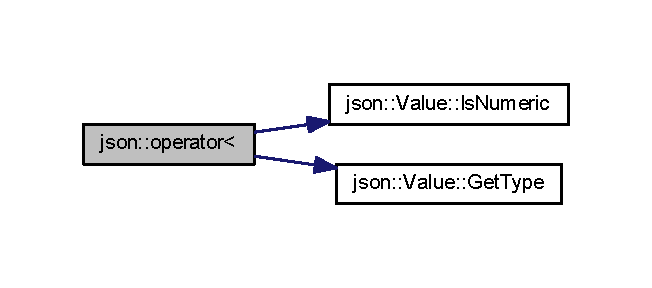
\includegraphics[width=313pt]{namespacejson_a820a993ff6009ec4eda8c4eb95ed1454_cgraph}
\end{center}
\end{figure}


\index{json@{json}!operator==@{operator==}}
\index{operator==@{operator==}!json@{json}}
\subsubsection[{operator==}]{\setlength{\rightskip}{0pt plus 5cm}bool json\+::operator== (
\begin{DoxyParamCaption}
\item[{const {\bf Object} \&}]{lhs, }
\item[{const {\bf Object} \&}]{rhs}
\end{DoxyParamCaption}
)\hspace{0.3cm}{\ttfamily [inline]}}\label{namespacejson_a1789077a8a1388991fe3ff3c3c04ca96}


Definition at line 492 of file json.\+h.

\index{json@{json}!operator==@{operator==}}
\index{operator==@{operator==}!json@{json}}
\subsubsection[{operator==}]{\setlength{\rightskip}{0pt plus 5cm}bool json\+::operator== (
\begin{DoxyParamCaption}
\item[{const {\bf Array} \&}]{lhs, }
\item[{const {\bf Array} \&}]{rhs}
\end{DoxyParamCaption}
)\hspace{0.3cm}{\ttfamily [inline]}}\label{namespacejson_a56bbe8bb376520a5db76f113283ca11e}


Definition at line 502 of file json.\+h.

\index{json@{json}!operator==@{operator==}}
\index{operator==@{operator==}!json@{json}}
\subsubsection[{operator==}]{\setlength{\rightskip}{0pt plus 5cm}bool json\+::operator== (
\begin{DoxyParamCaption}
\item[{const {\bf Value} \&}]{lhs, }
\item[{const {\bf Value} \&}]{rhs}
\end{DoxyParamCaption}
)\hspace{0.3cm}{\ttfamily [inline]}}\label{namespacejson_a7520c61ef1cc27c949ea957df799378c}


Definition at line 521 of file json.\+h.



Here is the call graph for this function\+:
\nopagebreak
\begin{figure}[H]
\begin{center}
\leavevmode
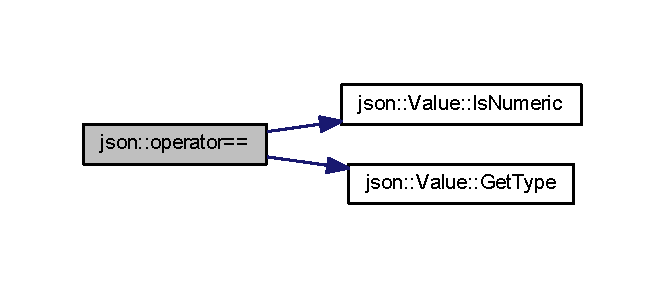
\includegraphics[width=319pt]{namespacejson_a7520c61ef1cc27c949ea957df799378c_cgraph}
\end{center}
\end{figure}


\index{json@{json}!Serialize@{Serialize}}
\index{Serialize@{Serialize}!json@{json}}
\subsubsection[{Serialize}]{\setlength{\rightskip}{0pt plus 5cm}std\+::string json\+::\+Serialize (
\begin{DoxyParamCaption}
\item[{const {\bf Value} \&}]{obj}
\end{DoxyParamCaption}
)}\label{namespacejson_a81467b49956c429d0196cadb03dd7fde}


Definition at line 544 of file json.\+cpp.



Here is the call graph for this function\+:
\nopagebreak
\begin{figure}[H]
\begin{center}
\leavevmode
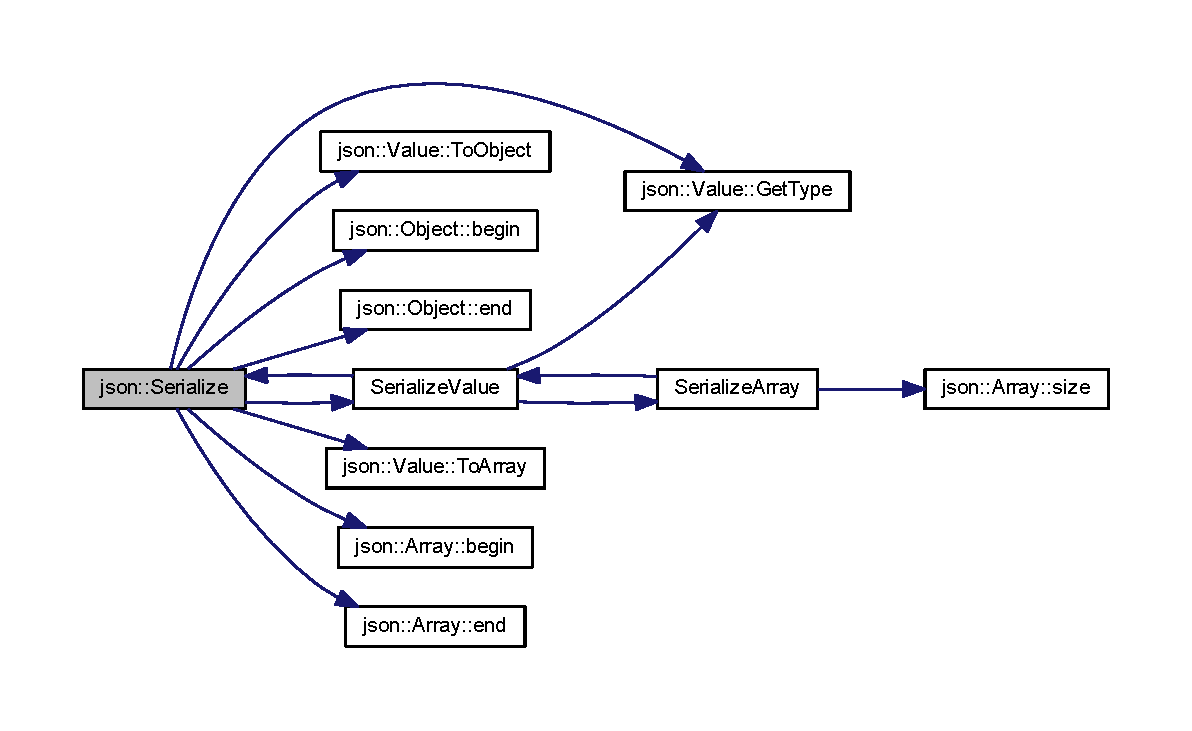
\includegraphics[width=350pt]{namespacejson_a81467b49956c429d0196cadb03dd7fde_cgraph}
\end{center}
\end{figure}



\chapter{Class Documentation}
\section{json\+:\+:Array Class Reference}
\label{classjson_1_1_array}\index{json\+::\+Array@{json\+::\+Array}}


{\ttfamily \#include $<$json.\+h$>$}

\subsection*{Public Types}
\begin{DoxyCompactItemize}
\item 
typedef std\+::vector$<$ {\bf Value} $>$ {\bf Value\+Vector}
\end{DoxyCompactItemize}
\subsection*{Public Member Functions}
\begin{DoxyCompactItemize}
\item 
{\bf Array} ()
\item 
{\bf Array} (const {\bf Array} \&a)
\item 
{\bf Array} \& {\bf operator=} (const {\bf Array} \&a)
\item 
{\bf Value} \& {\bf operator[$\,$]} (size\+\_\+t i)
\item 
const {\bf Value} \& {\bf operator[$\,$]} (size\+\_\+t i) const 
\item 
Value\+Vector\+::const\+\_\+iterator {\bf begin} () const 
\item 
Value\+Vector\+::const\+\_\+iterator {\bf end} () const 
\item 
Value\+Vector\+::iterator {\bf begin} ()
\item 
Value\+Vector\+::iterator {\bf end} ()
\item 
Value\+Vector\+::iterator {\bf find} (const {\bf Value} \&v)
\item 
Value\+Vector\+::const\+\_\+iterator {\bf find} (const {\bf Value} \&v) const 
\item 
bool {\bf Has\+Value} (const {\bf Value} \&v) const 
\item 
void {\bf Clear} ()
\item 
void {\bf push\+\_\+back} (const {\bf Value} \&v)
\item 
void {\bf insert} (size\+\_\+t index, const {\bf Value} \&v)
\item 
size\+\_\+t {\bf size} () const 
\end{DoxyCompactItemize}
\subsection*{Protected Attributes}
\begin{DoxyCompactItemize}
\item 
{\bf Value\+Vector} {\bf m\+Values}
\end{DoxyCompactItemize}
\subsection*{Friends}
\begin{DoxyCompactItemize}
\item 
bool {\bf operator==} (const {\bf Array} \&lhs, const {\bf Array} \&rhs)
\item 
bool {\bf operator!=} (const {\bf Array} \&lhs, const {\bf Array} \&rhs)
\item 
bool {\bf operator$<$} (const {\bf Array} \&lhs, const {\bf Array} \&rhs)
\item 
bool {\bf operator$>$} (const {\bf Array} \&lhs, const {\bf Array} \&rhs)
\item 
bool {\bf operator$<$=} (const {\bf Array} \&lhs, const {\bf Array} \&rhs)
\item 
bool {\bf operator$>$=} (const {\bf Array} \&lhs, const {\bf Array} \&rhs)
\end{DoxyCompactItemize}


\subsection{Detailed Description}


Definition at line 324 of file json.\+h.



\subsection{Member Typedef Documentation}
\index{json\+::\+Array@{json\+::\+Array}!Value\+Vector@{Value\+Vector}}
\index{Value\+Vector@{Value\+Vector}!json\+::\+Array@{json\+::\+Array}}
\subsubsection[{Value\+Vector}]{\setlength{\rightskip}{0pt plus 5cm}typedef std\+::vector$<${\bf Value}$>$ {\bf json\+::\+Array\+::\+Value\+Vector}}\label{classjson_1_1_array_a9980cfbe25d0da308156cf489d86b1a9}


Definition at line 331 of file json.\+h.



\subsection{Constructor \& Destructor Documentation}
\index{json\+::\+Array@{json\+::\+Array}!Array@{Array}}
\index{Array@{Array}!json\+::\+Array@{json\+::\+Array}}
\subsubsection[{Array}]{\setlength{\rightskip}{0pt plus 5cm}Array\+::\+Array (
\begin{DoxyParamCaption}
{}
\end{DoxyParamCaption}
)}\label{classjson_1_1_array_ae20b3dbb4aa6083679c0dea835abd861}


Definition at line 309 of file json.\+cpp.

\index{json\+::\+Array@{json\+::\+Array}!Array@{Array}}
\index{Array@{Array}!json\+::\+Array@{json\+::\+Array}}
\subsubsection[{Array}]{\setlength{\rightskip}{0pt plus 5cm}Array\+::\+Array (
\begin{DoxyParamCaption}
\item[{const {\bf Array} \&}]{a}
\end{DoxyParamCaption}
)}\label{classjson_1_1_array_a03f59ac3974d3462a5f1956498bcc4f7}


Definition at line 313 of file json.\+cpp.



\subsection{Member Function Documentation}
\index{json\+::\+Array@{json\+::\+Array}!begin@{begin}}
\index{begin@{begin}!json\+::\+Array@{json\+::\+Array}}
\subsubsection[{begin}]{\setlength{\rightskip}{0pt plus 5cm}Array\+::\+Value\+Vector\+::const\+\_\+iterator Array\+::begin (
\begin{DoxyParamCaption}
{}
\end{DoxyParamCaption}
) const}\label{classjson_1_1_array_a96107b61f986457da99341f08e0d98a0}


Definition at line 339 of file json.\+cpp.

\index{json\+::\+Array@{json\+::\+Array}!begin@{begin}}
\index{begin@{begin}!json\+::\+Array@{json\+::\+Array}}
\subsubsection[{begin}]{\setlength{\rightskip}{0pt plus 5cm}Array\+::\+Value\+Vector\+::iterator Array\+::begin (
\begin{DoxyParamCaption}
{}
\end{DoxyParamCaption}
)}\label{classjson_1_1_array_a2bcb20f9204852c74b836fe621f86843}


Definition at line 349 of file json.\+cpp.

\index{json\+::\+Array@{json\+::\+Array}!Clear@{Clear}}
\index{Clear@{Clear}!json\+::\+Array@{json\+::\+Array}}
\subsubsection[{Clear}]{\setlength{\rightskip}{0pt plus 5cm}void Array\+::\+Clear (
\begin{DoxyParamCaption}
{}
\end{DoxyParamCaption}
)}\label{classjson_1_1_array_ac6e5d254878a9a15018389857e88edef}


Definition at line 374 of file json.\+cpp.

\index{json\+::\+Array@{json\+::\+Array}!end@{end}}
\index{end@{end}!json\+::\+Array@{json\+::\+Array}}
\subsubsection[{end}]{\setlength{\rightskip}{0pt plus 5cm}Array\+::\+Value\+Vector\+::const\+\_\+iterator Array\+::end (
\begin{DoxyParamCaption}
{}
\end{DoxyParamCaption}
) const}\label{classjson_1_1_array_a4fc36b2ad3cac9d57c4a12f92aea668c}


Definition at line 344 of file json.\+cpp.

\index{json\+::\+Array@{json\+::\+Array}!end@{end}}
\index{end@{end}!json\+::\+Array@{json\+::\+Array}}
\subsubsection[{end}]{\setlength{\rightskip}{0pt plus 5cm}Array\+::\+Value\+Vector\+::iterator Array\+::end (
\begin{DoxyParamCaption}
{}
\end{DoxyParamCaption}
)}\label{classjson_1_1_array_a81f9a51107d41ce4edaa932afae80a75}


Definition at line 354 of file json.\+cpp.

\index{json\+::\+Array@{json\+::\+Array}!find@{find}}
\index{find@{find}!json\+::\+Array@{json\+::\+Array}}
\subsubsection[{find}]{\setlength{\rightskip}{0pt plus 5cm}Array\+::\+Value\+Vector\+::iterator Array\+::find (
\begin{DoxyParamCaption}
\item[{const {\bf Value} \&}]{v}
\end{DoxyParamCaption}
)}\label{classjson_1_1_array_a846c362ebd65439a5a7dde9c5e9b32ff}


Definition at line 379 of file json.\+cpp.

\index{json\+::\+Array@{json\+::\+Array}!find@{find}}
\index{find@{find}!json\+::\+Array@{json\+::\+Array}}
\subsubsection[{find}]{\setlength{\rightskip}{0pt plus 5cm}Array\+::\+Value\+Vector\+::const\+\_\+iterator Array\+::find (
\begin{DoxyParamCaption}
\item[{const {\bf Value} \&}]{v}
\end{DoxyParamCaption}
) const}\label{classjson_1_1_array_aaafe02d0f972088942cff746b99dfdef}


Definition at line 384 of file json.\+cpp.

\index{json\+::\+Array@{json\+::\+Array}!Has\+Value@{Has\+Value}}
\index{Has\+Value@{Has\+Value}!json\+::\+Array@{json\+::\+Array}}
\subsubsection[{Has\+Value}]{\setlength{\rightskip}{0pt plus 5cm}bool Array\+::\+Has\+Value (
\begin{DoxyParamCaption}
\item[{const {\bf Value} \&}]{v}
\end{DoxyParamCaption}
) const}\label{classjson_1_1_array_a78ecc1c676d3571dbf9738f6f4300bd8}


Definition at line 389 of file json.\+cpp.



Here is the call graph for this function\+:
\nopagebreak
\begin{figure}[H]
\begin{center}
\leavevmode
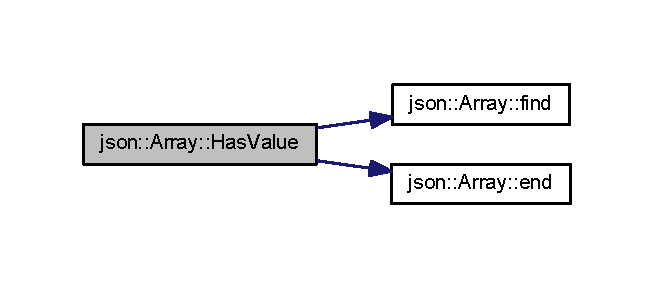
\includegraphics[width=314pt]{classjson_1_1_array_a78ecc1c676d3571dbf9738f6f4300bd8_cgraph}
\end{center}
\end{figure}


\index{json\+::\+Array@{json\+::\+Array}!insert@{insert}}
\index{insert@{insert}!json\+::\+Array@{json\+::\+Array}}
\subsubsection[{insert}]{\setlength{\rightskip}{0pt plus 5cm}void Array\+::insert (
\begin{DoxyParamCaption}
\item[{size\+\_\+t}]{index, }
\item[{const {\bf Value} \&}]{v}
\end{DoxyParamCaption}
)}\label{classjson_1_1_array_a0d1db900eecf2c019b028879b1966d72}


Definition at line 364 of file json.\+cpp.

\index{json\+::\+Array@{json\+::\+Array}!operator=@{operator=}}
\index{operator=@{operator=}!json\+::\+Array@{json\+::\+Array}}
\subsubsection[{operator=}]{\setlength{\rightskip}{0pt plus 5cm}{\bf Array} \& Array\+::operator= (
\begin{DoxyParamCaption}
\item[{const {\bf Array} \&}]{a}
\end{DoxyParamCaption}
)}\label{classjson_1_1_array_aa8c368d03d33e248e3d96b4977d2c495}


Definition at line 317 of file json.\+cpp.



Here is the call graph for this function\+:
\nopagebreak
\begin{figure}[H]
\begin{center}
\leavevmode
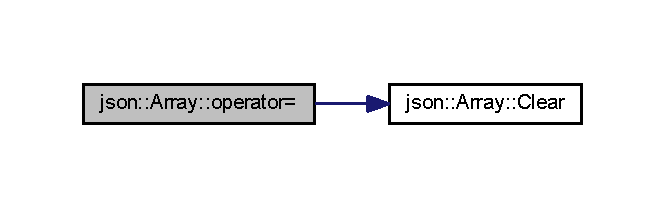
\includegraphics[width=319pt]{classjson_1_1_array_aa8c368d03d33e248e3d96b4977d2c495_cgraph}
\end{center}
\end{figure}


\index{json\+::\+Array@{json\+::\+Array}!operator[$\,$]@{operator[]}}
\index{operator[$\,$]@{operator[]}!json\+::\+Array@{json\+::\+Array}}
\subsubsection[{operator[]}]{\setlength{\rightskip}{0pt plus 5cm}{\bf Value} \& Array\+::operator[$\,$] (
\begin{DoxyParamCaption}
\item[{size\+\_\+t}]{i}
\end{DoxyParamCaption}
)}\label{classjson_1_1_array_ac3d31a0bbfeb5d23bc6dc2ac81cbf6b5}


Definition at line 328 of file json.\+cpp.

\index{json\+::\+Array@{json\+::\+Array}!operator[$\,$]@{operator[]}}
\index{operator[$\,$]@{operator[]}!json\+::\+Array@{json\+::\+Array}}
\subsubsection[{operator[]}]{\setlength{\rightskip}{0pt plus 5cm}const {\bf Value} \& Array\+::operator[$\,$] (
\begin{DoxyParamCaption}
\item[{size\+\_\+t}]{i}
\end{DoxyParamCaption}
) const}\label{classjson_1_1_array_a46c3c1f009769b7fce1276972dadc386}


Definition at line 333 of file json.\+cpp.

\index{json\+::\+Array@{json\+::\+Array}!push\+\_\+back@{push\+\_\+back}}
\index{push\+\_\+back@{push\+\_\+back}!json\+::\+Array@{json\+::\+Array}}
\subsubsection[{push\+\_\+back}]{\setlength{\rightskip}{0pt plus 5cm}void Array\+::push\+\_\+back (
\begin{DoxyParamCaption}
\item[{const {\bf Value} \&}]{v}
\end{DoxyParamCaption}
)}\label{classjson_1_1_array_ae0250880d436a0fa5aa3671ee54cbff8}


Definition at line 359 of file json.\+cpp.

\index{json\+::\+Array@{json\+::\+Array}!size@{size}}
\index{size@{size}!json\+::\+Array@{json\+::\+Array}}
\subsubsection[{size}]{\setlength{\rightskip}{0pt plus 5cm}size\+\_\+t Array\+::size (
\begin{DoxyParamCaption}
{}
\end{DoxyParamCaption}
) const}\label{classjson_1_1_array_a22978bd335f1c97e8448fca782e09420}


Definition at line 369 of file json.\+cpp.



\subsection{Friends And Related Function Documentation}
\index{json\+::\+Array@{json\+::\+Array}!operator"!=@{operator"!=}}
\index{operator"!=@{operator"!=}!json\+::\+Array@{json\+::\+Array}}
\subsubsection[{operator"!=}]{\setlength{\rightskip}{0pt plus 5cm}bool operator!= (
\begin{DoxyParamCaption}
\item[{const {\bf Array} \&}]{lhs, }
\item[{const {\bf Array} \&}]{rhs}
\end{DoxyParamCaption}
)\hspace{0.3cm}{\ttfamily [friend]}}\label{classjson_1_1_array_abcd1fdae411433dfd352fe5e9aecaa7a}


Definition at line 345 of file json.\+h.

\index{json\+::\+Array@{json\+::\+Array}!operator$<$@{operator$<$}}
\index{operator$<$@{operator$<$}!json\+::\+Array@{json\+::\+Array}}
\subsubsection[{operator$<$}]{\setlength{\rightskip}{0pt plus 5cm}bool operator$<$ (
\begin{DoxyParamCaption}
\item[{const {\bf Array} \&}]{lhs, }
\item[{const {\bf Array} \&}]{rhs}
\end{DoxyParamCaption}
)\hspace{0.3cm}{\ttfamily [friend]}}\label{classjson_1_1_array_a63deeecf801827e4b05e0270e787fb37}


Definition at line 507 of file json.\+h.

\index{json\+::\+Array@{json\+::\+Array}!operator$<$=@{operator$<$=}}
\index{operator$<$=@{operator$<$=}!json\+::\+Array@{json\+::\+Array}}
\subsubsection[{operator$<$=}]{\setlength{\rightskip}{0pt plus 5cm}bool operator$<$= (
\begin{DoxyParamCaption}
\item[{const {\bf Array} \&}]{lhs, }
\item[{const {\bf Array} \&}]{rhs}
\end{DoxyParamCaption}
)\hspace{0.3cm}{\ttfamily [friend]}}\label{classjson_1_1_array_ab353726ade4adcbe93ff219cd51e77b7}


Definition at line 348 of file json.\+h.

\index{json\+::\+Array@{json\+::\+Array}!operator==@{operator==}}
\index{operator==@{operator==}!json\+::\+Array@{json\+::\+Array}}
\subsubsection[{operator==}]{\setlength{\rightskip}{0pt plus 5cm}bool operator== (
\begin{DoxyParamCaption}
\item[{const {\bf Array} \&}]{lhs, }
\item[{const {\bf Array} \&}]{rhs}
\end{DoxyParamCaption}
)\hspace{0.3cm}{\ttfamily [friend]}}\label{classjson_1_1_array_a5eac737578730879ef9b00151a600127}


Definition at line 502 of file json.\+h.

\index{json\+::\+Array@{json\+::\+Array}!operator$>$@{operator$>$}}
\index{operator$>$@{operator$>$}!json\+::\+Array@{json\+::\+Array}}
\subsubsection[{operator$>$}]{\setlength{\rightskip}{0pt plus 5cm}bool operator$>$ (
\begin{DoxyParamCaption}
\item[{const {\bf Array} \&}]{lhs, }
\item[{const {\bf Array} \&}]{rhs}
\end{DoxyParamCaption}
)\hspace{0.3cm}{\ttfamily [friend]}}\label{classjson_1_1_array_adaf4ad9e358a52ce82a2be54b1543f95}


Definition at line 347 of file json.\+h.

\index{json\+::\+Array@{json\+::\+Array}!operator$>$=@{operator$>$=}}
\index{operator$>$=@{operator$>$=}!json\+::\+Array@{json\+::\+Array}}
\subsubsection[{operator$>$=}]{\setlength{\rightskip}{0pt plus 5cm}bool operator$>$= (
\begin{DoxyParamCaption}
\item[{const {\bf Array} \&}]{lhs, }
\item[{const {\bf Array} \&}]{rhs}
\end{DoxyParamCaption}
)\hspace{0.3cm}{\ttfamily [friend]}}\label{classjson_1_1_array_a66aa6acae48cac1ae12ac71613d5b882}


Definition at line 349 of file json.\+h.



\subsection{Member Data Documentation}
\index{json\+::\+Array@{json\+::\+Array}!m\+Values@{m\+Values}}
\index{m\+Values@{m\+Values}!json\+::\+Array@{json\+::\+Array}}
\subsubsection[{m\+Values}]{\setlength{\rightskip}{0pt plus 5cm}{\bf Value\+Vector} json\+::\+Array\+::m\+Values\hspace{0.3cm}{\ttfamily [protected]}}\label{classjson_1_1_array_a6c2619851ee6b74a0ca4d1d8dc49f7cd}


Definition at line 335 of file json.\+h.



The documentation for this class was generated from the following files\+:\begin{DoxyCompactItemize}
\item 
{\bf json.\+h}\item 
{\bf json.\+cpp}\end{DoxyCompactItemize}

\section{json\+:\+:Object Class Reference}
\label{classjson_1_1_object}\index{json\+::\+Object@{json\+::\+Object}}


{\ttfamily \#include $<$json.\+h$>$}

\subsection*{Public Types}
\begin{DoxyCompactItemize}
\item 
typedef std\+::map$<$ std\+::string, {\bf Value} $>$ {\bf Value\+Map}
\end{DoxyCompactItemize}
\subsection*{Public Member Functions}
\begin{DoxyCompactItemize}
\item 
{\bf Object} ()
\item 
{\bf Object} (const {\bf Object} \&obj)
\item 
{\bf Object} \& {\bf operator=} (const {\bf Object} \&obj)
\item 
{\bf Value} \& {\bf operator[$\,$]} (const std\+::string \&key)
\item 
const {\bf Value} \& {\bf operator[$\,$]} (const std\+::string \&key) const 
\item 
{\bf Value} \& {\bf operator[$\,$]} (const char $\ast$key)
\item 
const {\bf Value} \& {\bf operator[$\,$]} (const char $\ast$key) const 
\item 
Value\+Map\+::const\+\_\+iterator {\bf begin} () const 
\item 
Value\+Map\+::const\+\_\+iterator {\bf end} () const 
\item 
Value\+Map\+::iterator {\bf begin} ()
\item 
Value\+Map\+::iterator {\bf end} ()
\item 
Value\+Map\+::iterator {\bf find} (const std\+::string \&key)
\item 
Value\+Map\+::const\+\_\+iterator {\bf find} (const std\+::string \&key) const 
\item 
bool {\bf Has\+Key} (const std\+::string \&key) const 
\item 
int {\bf Has\+Keys} (const std\+::vector$<$ std\+::string $>$ \&keys) const 
\item 
int {\bf Has\+Keys} (const char $\ast$keys[$\,$], int key\+\_\+count) const 
\item 
void {\bf Clear} ()
\item 
size\+\_\+t {\bf size} () const 
\end{DoxyCompactItemize}
\subsection*{Protected Attributes}
\begin{DoxyCompactItemize}
\item 
{\bf Value\+Map} {\bf m\+Values}
\end{DoxyCompactItemize}
\subsection*{Friends}
\begin{DoxyCompactItemize}
\item 
bool {\bf operator==} (const {\bf Object} \&lhs, const {\bf Object} \&rhs)
\item 
bool {\bf operator!=} (const {\bf Object} \&lhs, const {\bf Object} \&rhs)
\item 
bool {\bf operator$<$} (const {\bf Object} \&lhs, const {\bf Object} \&rhs)
\item 
bool {\bf operator$>$} (const {\bf Object} \&lhs, const {\bf Object} \&rhs)
\item 
bool {\bf operator$<$=} (const {\bf Object} \&lhs, const {\bf Object} \&rhs)
\item 
bool {\bf operator$>$=} (const {\bf Object} \&lhs, const {\bf Object} \&rhs)
\end{DoxyCompactItemize}


\subsection{Detailed Description}


Definition at line 261 of file json.\+h.



\subsection{Member Typedef Documentation}
\index{json\+::\+Object@{json\+::\+Object}!Value\+Map@{Value\+Map}}
\index{Value\+Map@{Value\+Map}!json\+::\+Object@{json\+::\+Object}}
\subsubsection[{Value\+Map}]{\setlength{\rightskip}{0pt plus 5cm}typedef std\+::map$<$std\+::string, {\bf Value}$>$ {\bf json\+::\+Object\+::\+Value\+Map}}\label{classjson_1_1_object_aa4954dea50da7a887b6d9200408b0558}


Definition at line 268 of file json.\+h.



\subsection{Constructor \& Destructor Documentation}
\index{json\+::\+Object@{json\+::\+Object}!Object@{Object}}
\index{Object@{Object}!json\+::\+Object@{json\+::\+Object}}
\subsubsection[{Object}]{\setlength{\rightskip}{0pt plus 5cm}Object\+::\+Object (
\begin{DoxyParamCaption}
{}
\end{DoxyParamCaption}
)}\label{classjson_1_1_object_a40860402e64d8008fb42329df7097cdb}


Definition at line 396 of file json.\+cpp.

\index{json\+::\+Object@{json\+::\+Object}!Object@{Object}}
\index{Object@{Object}!json\+::\+Object@{json\+::\+Object}}
\subsubsection[{Object}]{\setlength{\rightskip}{0pt plus 5cm}Object\+::\+Object (
\begin{DoxyParamCaption}
\item[{const {\bf Object} \&}]{obj}
\end{DoxyParamCaption}
)}\label{classjson_1_1_object_a323f6dc88a65b7366b8b911f7ff24c21}


Definition at line 400 of file json.\+cpp.



\subsection{Member Function Documentation}
\index{json\+::\+Object@{json\+::\+Object}!begin@{begin}}
\index{begin@{begin}!json\+::\+Object@{json\+::\+Object}}
\subsubsection[{begin}]{\setlength{\rightskip}{0pt plus 5cm}Object\+::\+Value\+Map\+::const\+\_\+iterator Object\+::begin (
\begin{DoxyParamCaption}
{}
\end{DoxyParamCaption}
) const}\label{classjson_1_1_object_ae3135f6bc45ae944b272b819ec6880c9}


Definition at line 438 of file json.\+cpp.

\index{json\+::\+Object@{json\+::\+Object}!begin@{begin}}
\index{begin@{begin}!json\+::\+Object@{json\+::\+Object}}
\subsubsection[{begin}]{\setlength{\rightskip}{0pt plus 5cm}Object\+::\+Value\+Map\+::iterator Object\+::begin (
\begin{DoxyParamCaption}
{}
\end{DoxyParamCaption}
)}\label{classjson_1_1_object_ad4d61ef1cbea5189b669d468596128fb}


Definition at line 448 of file json.\+cpp.

\index{json\+::\+Object@{json\+::\+Object}!Clear@{Clear}}
\index{Clear@{Clear}!json\+::\+Object@{json\+::\+Object}}
\subsubsection[{Clear}]{\setlength{\rightskip}{0pt plus 5cm}void Object\+::\+Clear (
\begin{DoxyParamCaption}
{}
\end{DoxyParamCaption}
)}\label{classjson_1_1_object_a5b25442efcce1e5768e3790b36accd1a}


Definition at line 493 of file json.\+cpp.

\index{json\+::\+Object@{json\+::\+Object}!end@{end}}
\index{end@{end}!json\+::\+Object@{json\+::\+Object}}
\subsubsection[{end}]{\setlength{\rightskip}{0pt plus 5cm}Object\+::\+Value\+Map\+::const\+\_\+iterator Object\+::end (
\begin{DoxyParamCaption}
{}
\end{DoxyParamCaption}
) const}\label{classjson_1_1_object_a7a6cfa53a6b0cf2c4713bb74bcd1a3cc}


Definition at line 443 of file json.\+cpp.

\index{json\+::\+Object@{json\+::\+Object}!end@{end}}
\index{end@{end}!json\+::\+Object@{json\+::\+Object}}
\subsubsection[{end}]{\setlength{\rightskip}{0pt plus 5cm}Object\+::\+Value\+Map\+::iterator Object\+::end (
\begin{DoxyParamCaption}
{}
\end{DoxyParamCaption}
)}\label{classjson_1_1_object_a5002fe14bf3af8f44aacfaf963010e50}


Definition at line 453 of file json.\+cpp.

\index{json\+::\+Object@{json\+::\+Object}!find@{find}}
\index{find@{find}!json\+::\+Object@{json\+::\+Object}}
\subsubsection[{find}]{\setlength{\rightskip}{0pt plus 5cm}Object\+::\+Value\+Map\+::iterator Object\+::find (
\begin{DoxyParamCaption}
\item[{const std\+::string \&}]{key}
\end{DoxyParamCaption}
)}\label{classjson_1_1_object_a2a54f30c42a154665d45209de2c10080}


Definition at line 458 of file json.\+cpp.

\index{json\+::\+Object@{json\+::\+Object}!find@{find}}
\index{find@{find}!json\+::\+Object@{json\+::\+Object}}
\subsubsection[{find}]{\setlength{\rightskip}{0pt plus 5cm}Object\+::\+Value\+Map\+::const\+\_\+iterator Object\+::find (
\begin{DoxyParamCaption}
\item[{const std\+::string \&}]{key}
\end{DoxyParamCaption}
) const}\label{classjson_1_1_object_a37c490364fe7a0b5bbc2c9c7ca8bf5fd}


Definition at line 463 of file json.\+cpp.

\index{json\+::\+Object@{json\+::\+Object}!Has\+Key@{Has\+Key}}
\index{Has\+Key@{Has\+Key}!json\+::\+Object@{json\+::\+Object}}
\subsubsection[{Has\+Key}]{\setlength{\rightskip}{0pt plus 5cm}bool Object\+::\+Has\+Key (
\begin{DoxyParamCaption}
\item[{const std\+::string \&}]{key}
\end{DoxyParamCaption}
) const}\label{classjson_1_1_object_a57b1aee66ef297a4c408e3447d54a6ef}


Definition at line 468 of file json.\+cpp.



Here is the call graph for this function\+:
\nopagebreak
\begin{figure}[H]
\begin{center}
\leavevmode
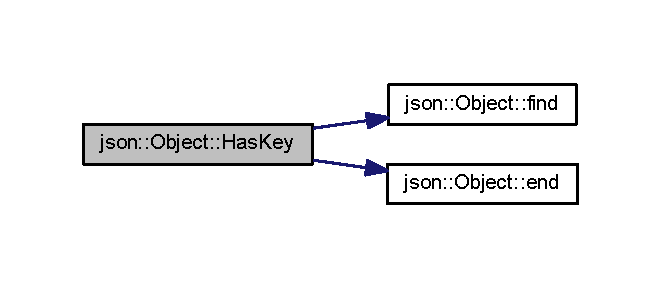
\includegraphics[width=317pt]{classjson_1_1_object_a57b1aee66ef297a4c408e3447d54a6ef_cgraph}
\end{center}
\end{figure}


\index{json\+::\+Object@{json\+::\+Object}!Has\+Keys@{Has\+Keys}}
\index{Has\+Keys@{Has\+Keys}!json\+::\+Object@{json\+::\+Object}}
\subsubsection[{Has\+Keys}]{\setlength{\rightskip}{0pt plus 5cm}int Object\+::\+Has\+Keys (
\begin{DoxyParamCaption}
\item[{const std\+::vector$<$ std\+::string $>$ \&}]{keys}
\end{DoxyParamCaption}
) const}\label{classjson_1_1_object_ad8935f41c775e463ebd111b25a33e7ac}


Definition at line 473 of file json.\+cpp.



Here is the call graph for this function\+:
\nopagebreak
\begin{figure}[H]
\begin{center}
\leavevmode
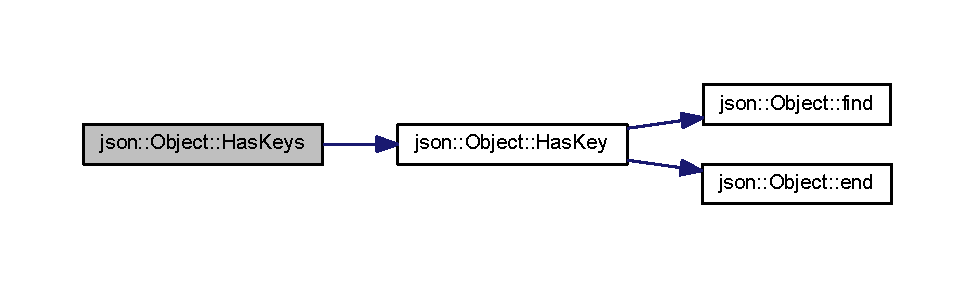
\includegraphics[width=350pt]{classjson_1_1_object_ad8935f41c775e463ebd111b25a33e7ac_cgraph}
\end{center}
\end{figure}


\index{json\+::\+Object@{json\+::\+Object}!Has\+Keys@{Has\+Keys}}
\index{Has\+Keys@{Has\+Keys}!json\+::\+Object@{json\+::\+Object}}
\subsubsection[{Has\+Keys}]{\setlength{\rightskip}{0pt plus 5cm}int json\+::\+Object\+::\+Has\+Keys (
\begin{DoxyParamCaption}
\item[{const char $\ast$}]{keys[$\,$], }
\item[{int}]{key\+\_\+count}
\end{DoxyParamCaption}
) const}\label{classjson_1_1_object_a9a9176f51ee4d9925c95ac380a88220f}
\index{json\+::\+Object@{json\+::\+Object}!operator=@{operator=}}
\index{operator=@{operator=}!json\+::\+Object@{json\+::\+Object}}
\subsubsection[{operator=}]{\setlength{\rightskip}{0pt plus 5cm}{\bf Object} \& Object\+::operator= (
\begin{DoxyParamCaption}
\item[{const {\bf Object} \&}]{obj}
\end{DoxyParamCaption}
)}\label{classjson_1_1_object_a21e49376c85da99a0e38ea546978f1e4}


Definition at line 405 of file json.\+cpp.



Here is the call graph for this function\+:
\nopagebreak
\begin{figure}[H]
\begin{center}
\leavevmode
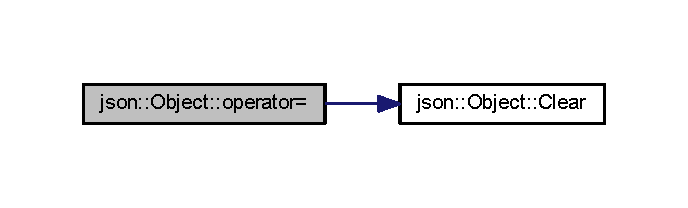
\includegraphics[width=330pt]{classjson_1_1_object_a21e49376c85da99a0e38ea546978f1e4_cgraph}
\end{center}
\end{figure}


\index{json\+::\+Object@{json\+::\+Object}!operator[$\,$]@{operator[]}}
\index{operator[$\,$]@{operator[]}!json\+::\+Object@{json\+::\+Object}}
\subsubsection[{operator[]}]{\setlength{\rightskip}{0pt plus 5cm}{\bf Value} \& Object\+::operator[$\,$] (
\begin{DoxyParamCaption}
\item[{const std\+::string \&}]{key}
\end{DoxyParamCaption}
)}\label{classjson_1_1_object_a56547ff2d63afd90b40627f38f0918ba}


Definition at line 416 of file json.\+cpp.

\index{json\+::\+Object@{json\+::\+Object}!operator[$\,$]@{operator[]}}
\index{operator[$\,$]@{operator[]}!json\+::\+Object@{json\+::\+Object}}
\subsubsection[{operator[]}]{\setlength{\rightskip}{0pt plus 5cm}const {\bf Value} \& Object\+::operator[$\,$] (
\begin{DoxyParamCaption}
\item[{const std\+::string \&}]{key}
\end{DoxyParamCaption}
) const}\label{classjson_1_1_object_ad7664c3133c35588f8bed83d4fa4b668}


Definition at line 421 of file json.\+cpp.

\index{json\+::\+Object@{json\+::\+Object}!operator[$\,$]@{operator[]}}
\index{operator[$\,$]@{operator[]}!json\+::\+Object@{json\+::\+Object}}
\subsubsection[{operator[]}]{\setlength{\rightskip}{0pt plus 5cm}{\bf Value} \& Object\+::operator[$\,$] (
\begin{DoxyParamCaption}
\item[{const char $\ast$}]{key}
\end{DoxyParamCaption}
)}\label{classjson_1_1_object_a4e4e29c681471a2da71a6dfc28de06ea}


Definition at line 427 of file json.\+cpp.

\index{json\+::\+Object@{json\+::\+Object}!operator[$\,$]@{operator[]}}
\index{operator[$\,$]@{operator[]}!json\+::\+Object@{json\+::\+Object}}
\subsubsection[{operator[]}]{\setlength{\rightskip}{0pt plus 5cm}const {\bf Value} \& Object\+::operator[$\,$] (
\begin{DoxyParamCaption}
\item[{const char $\ast$}]{key}
\end{DoxyParamCaption}
) const}\label{classjson_1_1_object_a23e6bb31047863c62d15f24d47930124}


Definition at line 432 of file json.\+cpp.

\index{json\+::\+Object@{json\+::\+Object}!size@{size}}
\index{size@{size}!json\+::\+Object@{json\+::\+Object}}
\subsubsection[{size}]{\setlength{\rightskip}{0pt plus 5cm}size\+\_\+t json\+::\+Object\+::size (
\begin{DoxyParamCaption}
{}
\end{DoxyParamCaption}
) const\hspace{0.3cm}{\ttfamily [inline]}}\label{classjson_1_1_object_ae5d4a190deef5a99b8d2685c97900030}


Definition at line 319 of file json.\+h.



\subsection{Friends And Related Function Documentation}
\index{json\+::\+Object@{json\+::\+Object}!operator"!=@{operator"!=}}
\index{operator"!=@{operator"!=}!json\+::\+Object@{json\+::\+Object}}
\subsubsection[{operator"!=}]{\setlength{\rightskip}{0pt plus 5cm}bool operator!= (
\begin{DoxyParamCaption}
\item[{const {\bf Object} \&}]{lhs, }
\item[{const {\bf Object} \&}]{rhs}
\end{DoxyParamCaption}
)\hspace{0.3cm}{\ttfamily [friend]}}\label{classjson_1_1_object_a44bd7c57009ffb99eb252af4cc060e5e}


Definition at line 282 of file json.\+h.

\index{json\+::\+Object@{json\+::\+Object}!operator$<$@{operator$<$}}
\index{operator$<$@{operator$<$}!json\+::\+Object@{json\+::\+Object}}
\subsubsection[{operator$<$}]{\setlength{\rightskip}{0pt plus 5cm}bool operator$<$ (
\begin{DoxyParamCaption}
\item[{const {\bf Object} \&}]{lhs, }
\item[{const {\bf Object} \&}]{rhs}
\end{DoxyParamCaption}
)\hspace{0.3cm}{\ttfamily [friend]}}\label{classjson_1_1_object_a652d6161403f67f951870946eda8503b}


Definition at line 497 of file json.\+h.

\index{json\+::\+Object@{json\+::\+Object}!operator$<$=@{operator$<$=}}
\index{operator$<$=@{operator$<$=}!json\+::\+Object@{json\+::\+Object}}
\subsubsection[{operator$<$=}]{\setlength{\rightskip}{0pt plus 5cm}bool operator$<$= (
\begin{DoxyParamCaption}
\item[{const {\bf Object} \&}]{lhs, }
\item[{const {\bf Object} \&}]{rhs}
\end{DoxyParamCaption}
)\hspace{0.3cm}{\ttfamily [friend]}}\label{classjson_1_1_object_a14a11dad5529b1b640771ae26498af83}


Definition at line 285 of file json.\+h.

\index{json\+::\+Object@{json\+::\+Object}!operator==@{operator==}}
\index{operator==@{operator==}!json\+::\+Object@{json\+::\+Object}}
\subsubsection[{operator==}]{\setlength{\rightskip}{0pt plus 5cm}bool operator== (
\begin{DoxyParamCaption}
\item[{const {\bf Object} \&}]{lhs, }
\item[{const {\bf Object} \&}]{rhs}
\end{DoxyParamCaption}
)\hspace{0.3cm}{\ttfamily [friend]}}\label{classjson_1_1_object_a5bf79317593848055dc650d41215bda1}


Definition at line 492 of file json.\+h.

\index{json\+::\+Object@{json\+::\+Object}!operator$>$@{operator$>$}}
\index{operator$>$@{operator$>$}!json\+::\+Object@{json\+::\+Object}}
\subsubsection[{operator$>$}]{\setlength{\rightskip}{0pt plus 5cm}bool operator$>$ (
\begin{DoxyParamCaption}
\item[{const {\bf Object} \&}]{lhs, }
\item[{const {\bf Object} \&}]{rhs}
\end{DoxyParamCaption}
)\hspace{0.3cm}{\ttfamily [friend]}}\label{classjson_1_1_object_a819f5485c06a00010c6d68833f2fd903}


Definition at line 284 of file json.\+h.

\index{json\+::\+Object@{json\+::\+Object}!operator$>$=@{operator$>$=}}
\index{operator$>$=@{operator$>$=}!json\+::\+Object@{json\+::\+Object}}
\subsubsection[{operator$>$=}]{\setlength{\rightskip}{0pt plus 5cm}bool operator$>$= (
\begin{DoxyParamCaption}
\item[{const {\bf Object} \&}]{lhs, }
\item[{const {\bf Object} \&}]{rhs}
\end{DoxyParamCaption}
)\hspace{0.3cm}{\ttfamily [friend]}}\label{classjson_1_1_object_a34be1225ba90528635030725d46a4977}


Definition at line 286 of file json.\+h.



\subsection{Member Data Documentation}
\index{json\+::\+Object@{json\+::\+Object}!m\+Values@{m\+Values}}
\index{m\+Values@{m\+Values}!json\+::\+Object@{json\+::\+Object}}
\subsubsection[{m\+Values}]{\setlength{\rightskip}{0pt plus 5cm}{\bf Value\+Map} json\+::\+Object\+::m\+Values\hspace{0.3cm}{\ttfamily [protected]}}\label{classjson_1_1_object_abd590583e6aec8e4e3635d38f809c60b}


Definition at line 272 of file json.\+h.



The documentation for this class was generated from the following files\+:\begin{DoxyCompactItemize}
\item 
{\bf json.\+h}\item 
{\bf json.\+cpp}\end{DoxyCompactItemize}

\section{S\+E\+Ambient\+Light$<$ T $>$ Class Template Reference}
\label{class_s_e_ambient_light}\index{S\+E\+Ambient\+Light$<$ T $>$@{S\+E\+Ambient\+Light$<$ T $>$}}


{\ttfamily \#include $<$S\+E\+Light.\+h$>$}



Inheritance diagram for S\+E\+Ambient\+Light$<$ T $>$\+:
\nopagebreak
\begin{figure}[H]
\begin{center}
\leavevmode
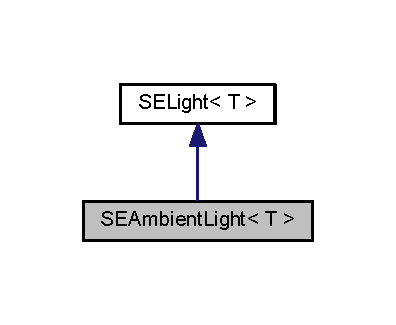
\includegraphics[width=190pt]{class_s_e_ambient_light__inherit__graph}
\end{center}
\end{figure}


Collaboration diagram for S\+E\+Ambient\+Light$<$ T $>$\+:
\nopagebreak
\begin{figure}[H]
\begin{center}
\leavevmode
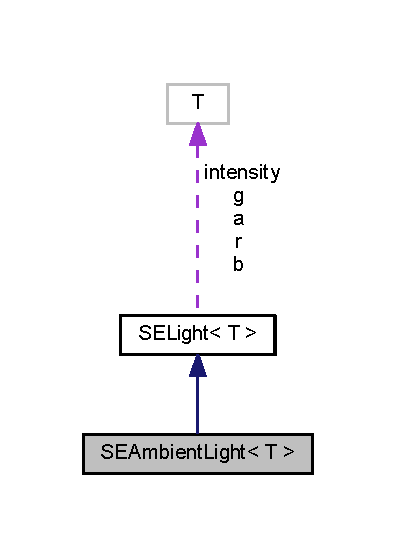
\includegraphics[width=190pt]{class_s_e_ambient_light__coll__graph}
\end{center}
\end{figure}
\subsection*{Protected Member Functions}
\begin{DoxyCompactItemize}
\item 
{\bf S\+E\+Ambient\+Light} ()
\item 
{\bf S\+E\+Ambient\+Light} (T {\bf r}, T {\bf g}, T {\bf b}, T {\bf a})
\item 
virtual {\bf $\sim$\+S\+E\+Ambient\+Light} ()
\end{DoxyCompactItemize}
\subsection*{Additional Inherited Members}


\subsection{Detailed Description}
\subsubsection*{template$<$class T$>$class S\+E\+Ambient\+Light$<$ T $>$}



Definition at line 54 of file S\+E\+Light.\+h.



\subsection{Constructor \& Destructor Documentation}
\index{S\+E\+Ambient\+Light@{S\+E\+Ambient\+Light}!S\+E\+Ambient\+Light@{S\+E\+Ambient\+Light}}
\index{S\+E\+Ambient\+Light@{S\+E\+Ambient\+Light}!S\+E\+Ambient\+Light@{S\+E\+Ambient\+Light}}
\subsubsection[{S\+E\+Ambient\+Light}]{\setlength{\rightskip}{0pt plus 5cm}template$<$class T$>$ {\bf S\+E\+Ambient\+Light}$<$ T $>$\+::{\bf S\+E\+Ambient\+Light} (
\begin{DoxyParamCaption}
{}
\end{DoxyParamCaption}
)\hspace{0.3cm}{\ttfamily [inline]}, {\ttfamily [protected]}}\label{class_s_e_ambient_light_a4a9a2b88e0baf3096ef84c384728c354}


Definition at line 58 of file S\+E\+Light.\+h.

\index{S\+E\+Ambient\+Light@{S\+E\+Ambient\+Light}!S\+E\+Ambient\+Light@{S\+E\+Ambient\+Light}}
\index{S\+E\+Ambient\+Light@{S\+E\+Ambient\+Light}!S\+E\+Ambient\+Light@{S\+E\+Ambient\+Light}}
\subsubsection[{S\+E\+Ambient\+Light}]{\setlength{\rightskip}{0pt plus 5cm}template$<$class T$>$ {\bf S\+E\+Ambient\+Light}$<$ T $>$\+::{\bf S\+E\+Ambient\+Light} (
\begin{DoxyParamCaption}
\item[{T}]{r, }
\item[{T}]{g, }
\item[{T}]{b, }
\item[{T}]{a}
\end{DoxyParamCaption}
)\hspace{0.3cm}{\ttfamily [inline]}, {\ttfamily [protected]}}\label{class_s_e_ambient_light_a44eaf89e78cb99580590579da8a79c0d}


Definition at line 59 of file S\+E\+Light.\+h.

\index{S\+E\+Ambient\+Light@{S\+E\+Ambient\+Light}!````~S\+E\+Ambient\+Light@{$\sim$\+S\+E\+Ambient\+Light}}
\index{````~S\+E\+Ambient\+Light@{$\sim$\+S\+E\+Ambient\+Light}!S\+E\+Ambient\+Light@{S\+E\+Ambient\+Light}}
\subsubsection[{$\sim$\+S\+E\+Ambient\+Light}]{\setlength{\rightskip}{0pt plus 5cm}template$<$class T$>$ virtual {\bf S\+E\+Ambient\+Light}$<$ T $>$\+::$\sim${\bf S\+E\+Ambient\+Light} (
\begin{DoxyParamCaption}
{}
\end{DoxyParamCaption}
)\hspace{0.3cm}{\ttfamily [inline]}, {\ttfamily [protected]}, {\ttfamily [virtual]}}\label{class_s_e_ambient_light_afaaca1b38399c28e1cc764039ef37c21}


Definition at line 60 of file S\+E\+Light.\+h.



The documentation for this class was generated from the following file\+:\begin{DoxyCompactItemize}
\item 
{\bf S\+E\+Light.\+h}\end{DoxyCompactItemize}

\section{S\+E\+Application$<$ T $>$ Class Template Reference}
\label{class_s_e_application}\index{S\+E\+Application$<$ T $>$@{S\+E\+Application$<$ T $>$}}


{\ttfamily \#include $<$S\+E\+Application.\+h$>$}



Inheritance diagram for S\+E\+Application$<$ T $>$\+:
\nopagebreak
\begin{figure}[H]
\begin{center}
\leavevmode
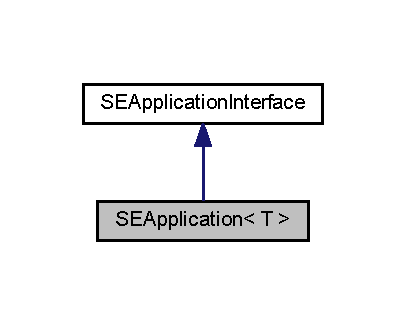
\includegraphics[width=195pt]{class_s_e_application__inherit__graph}
\end{center}
\end{figure}


Collaboration diagram for S\+E\+Application$<$ T $>$\+:
\nopagebreak
\begin{figure}[H]
\begin{center}
\leavevmode
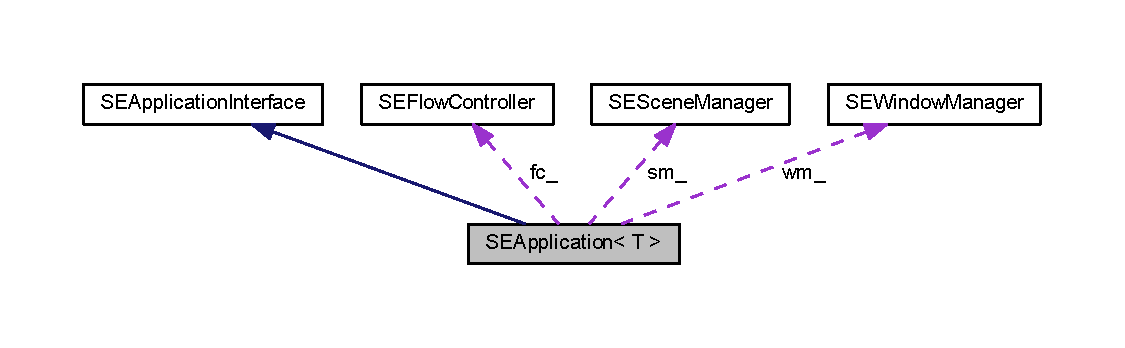
\includegraphics[width=350pt]{class_s_e_application__coll__graph}
\end{center}
\end{figure}
\subsection*{Public Member Functions}
\begin{DoxyCompactItemize}
\item 
virtual void {\bf init} (int argc, char $\ast$$\ast$argv)
\item 
virtual void {\bf run} ()
\item 
virtual void {\bf quit} ()
\item 
virtual {\bf $\sim$\+S\+E\+Application} ()
\item 
virtual {\bf S\+E\+Render\+Service} $\ast$ {\bf rs} ()
\item 
virtual {\bf S\+E\+Window\+Manager} $\ast$ {\bf wm} ()
\item 
virtual {\bf S\+E\+Flow\+Controller} $\ast$ {\bf fc} ()
\item 
virtual void {\bf display} ()
\item 
virtual void {\bf idle} ()
\end{DoxyCompactItemize}
\subsection*{Protected Member Functions}
\begin{DoxyCompactItemize}
\item 
{\bf S\+E\+Application} (std\+::string t)
\item 
{\bf S\+E\+Application} (const char $\ast$t)
\end{DoxyCompactItemize}
\subsection*{Protected Attributes}
\begin{DoxyCompactItemize}
\item 
std\+::string {\bf title\+\_\+}
\item 
{\bf S\+E\+Scene\+Manager} {\bf sm\+\_\+}
\item 
{\bf S\+E\+Render\+Service\+Internals}$<$ T $>$ $\ast$ {\bf rs\+\_\+}
\item 
{\bf S\+E\+Window\+Manager} $\ast$ {\bf wm\+\_\+}
\item 
{\bf S\+E\+Flow\+Controller} $\ast$ {\bf fc\+\_\+}
\end{DoxyCompactItemize}
\subsection*{Additional Inherited Members}


\subsection{Detailed Description}
\subsubsection*{template$<$class T$>$class S\+E\+Application$<$ T $>$}



Definition at line 18 of file S\+E\+Application.\+h.



\subsection{Constructor \& Destructor Documentation}
\index{S\+E\+Application@{S\+E\+Application}!````~S\+E\+Application@{$\sim$\+S\+E\+Application}}
\index{````~S\+E\+Application@{$\sim$\+S\+E\+Application}!S\+E\+Application@{S\+E\+Application}}
\subsubsection[{$\sim$\+S\+E\+Application}]{\setlength{\rightskip}{0pt plus 5cm}template$<$class T $>$ {\bf S\+E\+Application}$<$ T $>$\+::$\sim${\bf S\+E\+Application} (
\begin{DoxyParamCaption}
{}
\end{DoxyParamCaption}
)\hspace{0.3cm}{\ttfamily [virtual]}}\label{class_s_e_application_a6cead4e6a89d9c0b75683e539410ca14}


Definition at line 59 of file S\+E\+Application.\+h.



Here is the call graph for this function\+:
\nopagebreak
\begin{figure}[H]
\begin{center}
\leavevmode
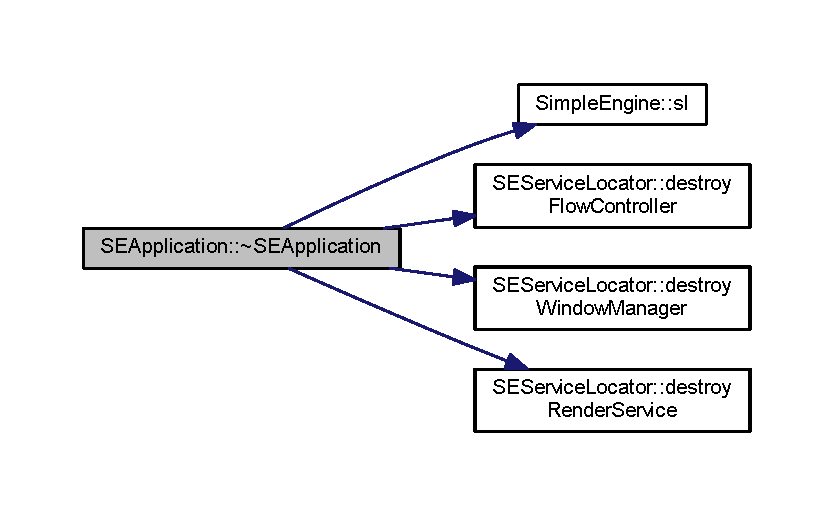
\includegraphics[width=350pt]{class_s_e_application_a6cead4e6a89d9c0b75683e539410ca14_cgraph}
\end{center}
\end{figure}


\index{S\+E\+Application@{S\+E\+Application}!S\+E\+Application@{S\+E\+Application}}
\index{S\+E\+Application@{S\+E\+Application}!S\+E\+Application@{S\+E\+Application}}
\subsubsection[{S\+E\+Application}]{\setlength{\rightskip}{0pt plus 5cm}template$<$class T$>$ {\bf S\+E\+Application}$<$ T $>$\+::{\bf S\+E\+Application} (
\begin{DoxyParamCaption}
\item[{std\+::string}]{t}
\end{DoxyParamCaption}
)\hspace{0.3cm}{\ttfamily [inline]}, {\ttfamily [protected]}}\label{class_s_e_application_a6a5f4e53420eb146d177a84cdc691655}


Definition at line 46 of file S\+E\+Application.\+h.

\index{S\+E\+Application@{S\+E\+Application}!S\+E\+Application@{S\+E\+Application}}
\index{S\+E\+Application@{S\+E\+Application}!S\+E\+Application@{S\+E\+Application}}
\subsubsection[{S\+E\+Application}]{\setlength{\rightskip}{0pt plus 5cm}template$<$class T$>$ {\bf S\+E\+Application}$<$ T $>$\+::{\bf S\+E\+Application} (
\begin{DoxyParamCaption}
\item[{const char $\ast$}]{t}
\end{DoxyParamCaption}
)\hspace{0.3cm}{\ttfamily [inline]}, {\ttfamily [protected]}}\label{class_s_e_application_a618938e04202c52914923a2af5e4c65a}


Definition at line 50 of file S\+E\+Application.\+h.



\subsection{Member Function Documentation}
\index{S\+E\+Application@{S\+E\+Application}!display@{display}}
\index{display@{display}!S\+E\+Application@{S\+E\+Application}}
\subsubsection[{display}]{\setlength{\rightskip}{0pt plus 5cm}template$<$class T$>$ virtual void {\bf S\+E\+Application}$<$ T $>$\+::display (
\begin{DoxyParamCaption}
{}
\end{DoxyParamCaption}
)\hspace{0.3cm}{\ttfamily [inline]}, {\ttfamily [virtual]}}\label{class_s_e_application_af68fb4de72017976c14e4e81a35f509f}


Implements {\bf S\+E\+Application\+Interface} \doxyref{}{p.}{class_s_e_application_interface_a7dbd81ef6669b220b75a190f5ac19d2c}.



Reimplemented in {\bf S\+E\+Test\+App1} \doxyref{}{p.}{class_s_e_test_app1_aa673ae83a7249cd54756a4a475594c18}, and {\bf S\+E\+Test\+App2} \doxyref{}{p.}{class_s_e_test_app2_a7d4d1ed4ffec940cffaa677638439dd0}.



Definition at line 34 of file S\+E\+Application.\+h.

\index{S\+E\+Application@{S\+E\+Application}!fc@{fc}}
\index{fc@{fc}!S\+E\+Application@{S\+E\+Application}}
\subsubsection[{fc}]{\setlength{\rightskip}{0pt plus 5cm}template$<$class T$>$ virtual {\bf S\+E\+Flow\+Controller}$\ast$ {\bf S\+E\+Application}$<$ T $>$\+::fc (
\begin{DoxyParamCaption}
{}
\end{DoxyParamCaption}
)\hspace{0.3cm}{\ttfamily [inline]}, {\ttfamily [virtual]}}\label{class_s_e_application_a8b62aedc2f6fee908272cb9b6638d87e}


Implements {\bf S\+E\+Application\+Interface} \doxyref{}{p.}{class_s_e_application_interface_aaf13d84e9c716f4fa7131f287f5e823b}.



Definition at line 32 of file S\+E\+Application.\+h.

\index{S\+E\+Application@{S\+E\+Application}!idle@{idle}}
\index{idle@{idle}!S\+E\+Application@{S\+E\+Application}}
\subsubsection[{idle}]{\setlength{\rightskip}{0pt plus 5cm}template$<$class T$>$ virtual void {\bf S\+E\+Application}$<$ T $>$\+::idle (
\begin{DoxyParamCaption}
{}
\end{DoxyParamCaption}
)\hspace{0.3cm}{\ttfamily [inline]}, {\ttfamily [virtual]}}\label{class_s_e_application_ae10739b2876ad09ee15590ba822e21eb}


Reimplemented from {\bf S\+E\+Application\+Interface} \doxyref{}{p.}{class_s_e_application_interface_ace0d1433d2f5b08c9cd582318eabcffc}.



Reimplemented in {\bf S\+E\+Test\+App1} \doxyref{}{p.}{class_s_e_test_app1_a2a3457e16ee71cba6aa71728ecd98045}, and {\bf S\+E\+Test\+App2} \doxyref{}{p.}{class_s_e_test_app2_a08d31acfd918a2ee16bff9fec0927b6d}.



Definition at line 35 of file S\+E\+Application.\+h.

\index{S\+E\+Application@{S\+E\+Application}!init@{init}}
\index{init@{init}!S\+E\+Application@{S\+E\+Application}}
\subsubsection[{init}]{\setlength{\rightskip}{0pt plus 5cm}template$<$class T $>$ void {\bf S\+E\+Application}$<$ T $>$\+::init (
\begin{DoxyParamCaption}
\item[{int}]{argc, }
\item[{char $\ast$$\ast$}]{argv}
\end{DoxyParamCaption}
)\hspace{0.3cm}{\ttfamily [virtual]}}\label{class_s_e_application_ae8453fdab08443b4a1c7fc9db1a4436e}


Implements {\bf S\+E\+Application\+Interface} \doxyref{}{p.}{class_s_e_application_interface_a6122d2fc9569a97ee0d69145a9a76779}.



Reimplemented in {\bf S\+E\+Test\+App1} \doxyref{}{p.}{class_s_e_test_app1_ac03290087ff6592a7d368edea13b66c9}, and {\bf S\+E\+Test\+App2} \doxyref{}{p.}{class_s_e_test_app2_a8b0e69df9de394aa9c21855570bb1d1d}.



Definition at line 66 of file S\+E\+Application.\+h.



Here is the call graph for this function\+:
\nopagebreak
\begin{figure}[H]
\begin{center}
\leavevmode
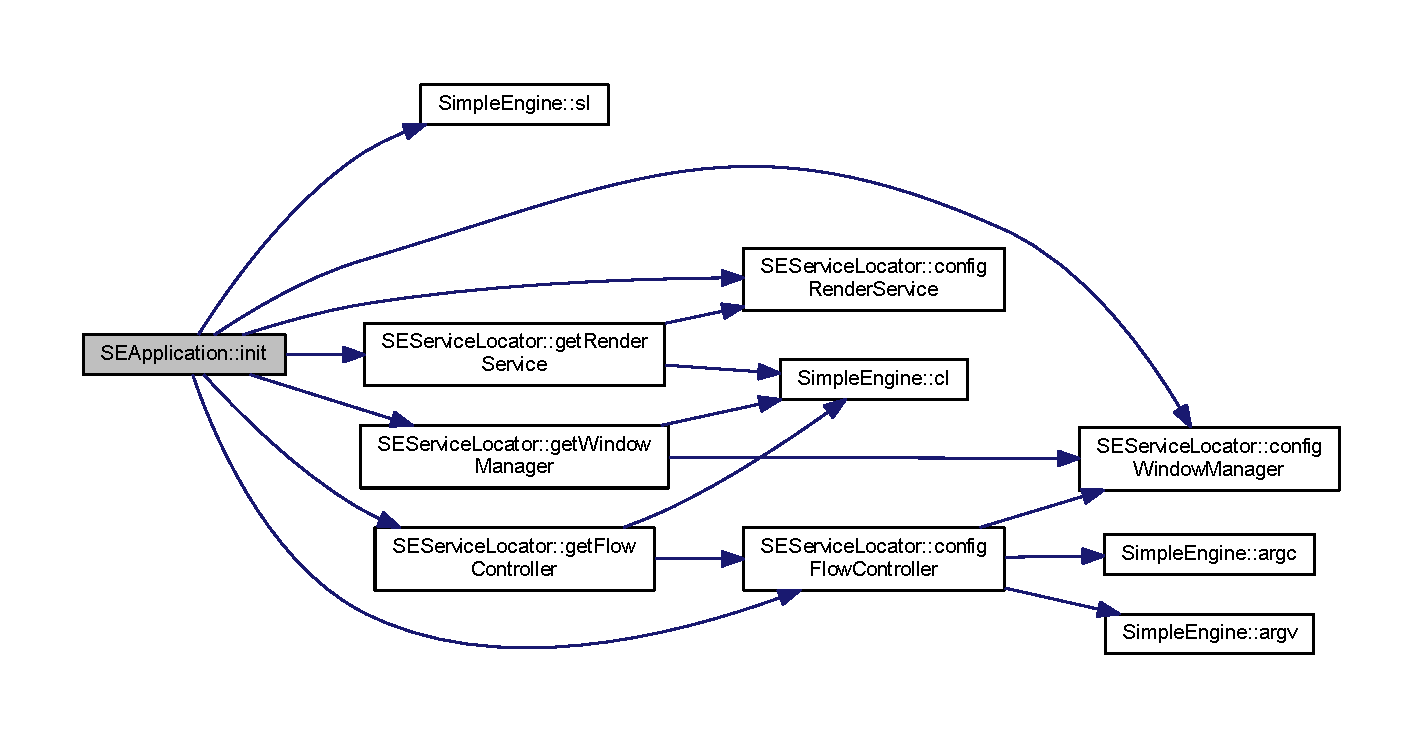
\includegraphics[width=350pt]{class_s_e_application_ae8453fdab08443b4a1c7fc9db1a4436e_cgraph}
\end{center}
\end{figure}


\index{S\+E\+Application@{S\+E\+Application}!quit@{quit}}
\index{quit@{quit}!S\+E\+Application@{S\+E\+Application}}
\subsubsection[{quit}]{\setlength{\rightskip}{0pt plus 5cm}template$<$class T $>$ void {\bf S\+E\+Application}$<$ T $>$\+::quit (
\begin{DoxyParamCaption}
{}
\end{DoxyParamCaption}
)\hspace{0.3cm}{\ttfamily [virtual]}}\label{class_s_e_application_a1d6dd2dd21b3e0ec2fb519c18be75456}


Implements {\bf S\+E\+Application\+Interface} \doxyref{}{p.}{class_s_e_application_interface_ac1c05e2c7c83d66e6c5dbe52b2bd681b}.



Reimplemented in {\bf S\+E\+Test\+App1} \doxyref{}{p.}{class_s_e_test_app1_adb78b0efdd9da9dc098d4ffa6828f727}, and {\bf S\+E\+Test\+App2} \doxyref{}{p.}{class_s_e_test_app2_ab11859c0ab08874e228654bde04b30d6}.



Definition at line 88 of file S\+E\+Application.\+h.

\index{S\+E\+Application@{S\+E\+Application}!rs@{rs}}
\index{rs@{rs}!S\+E\+Application@{S\+E\+Application}}
\subsubsection[{rs}]{\setlength{\rightskip}{0pt plus 5cm}template$<$class T$>$ virtual {\bf S\+E\+Render\+Service}$\ast$ {\bf S\+E\+Application}$<$ T $>$\+::rs (
\begin{DoxyParamCaption}
{}
\end{DoxyParamCaption}
)\hspace{0.3cm}{\ttfamily [inline]}, {\ttfamily [virtual]}}\label{class_s_e_application_accb31e9ba20aba3b9e87fdebe890b112}


Implements {\bf S\+E\+Application\+Interface} \doxyref{}{p.}{class_s_e_application_interface_a3f3ad17c66f7e5154c06a1b51c64f79b}.



Definition at line 30 of file S\+E\+Application.\+h.

\index{S\+E\+Application@{S\+E\+Application}!run@{run}}
\index{run@{run}!S\+E\+Application@{S\+E\+Application}}
\subsubsection[{run}]{\setlength{\rightskip}{0pt plus 5cm}template$<$class T $>$ void {\bf S\+E\+Application}$<$ T $>$\+::run (
\begin{DoxyParamCaption}
{}
\end{DoxyParamCaption}
)\hspace{0.3cm}{\ttfamily [virtual]}}\label{class_s_e_application_a1cb54d6b2e488ec96ec0bd743f73e68e}


Implements {\bf S\+E\+Application\+Interface} \doxyref{}{p.}{class_s_e_application_interface_a80314f1b5d2ee927f0aec52d2939a4e3}.



Reimplemented in {\bf S\+E\+Test\+App1} \doxyref{}{p.}{class_s_e_test_app1_ab3f47fe7c735bc68d2e18867011d33a2}, and {\bf S\+E\+Test\+App2} \doxyref{}{p.}{class_s_e_test_app2_a721c6c574531fcd0786bb8f39683dd7e}.



Definition at line 82 of file S\+E\+Application.\+h.

\index{S\+E\+Application@{S\+E\+Application}!wm@{wm}}
\index{wm@{wm}!S\+E\+Application@{S\+E\+Application}}
\subsubsection[{wm}]{\setlength{\rightskip}{0pt plus 5cm}template$<$class T$>$ virtual {\bf S\+E\+Window\+Manager}$\ast$ {\bf S\+E\+Application}$<$ T $>$\+::wm (
\begin{DoxyParamCaption}
{}
\end{DoxyParamCaption}
)\hspace{0.3cm}{\ttfamily [inline]}, {\ttfamily [virtual]}}\label{class_s_e_application_a06d1f50c567761756a3dcf30e5bddefc}


Implements {\bf S\+E\+Application\+Interface} \doxyref{}{p.}{class_s_e_application_interface_a741d9bee928dc78ea56fe6de72137393}.



Definition at line 31 of file S\+E\+Application.\+h.



\subsection{Member Data Documentation}
\index{S\+E\+Application@{S\+E\+Application}!fc\+\_\+@{fc\+\_\+}}
\index{fc\+\_\+@{fc\+\_\+}!S\+E\+Application@{S\+E\+Application}}
\subsubsection[{fc\+\_\+}]{\setlength{\rightskip}{0pt plus 5cm}template$<$class T$>$ {\bf S\+E\+Flow\+Controller}$\ast$ {\bf S\+E\+Application}$<$ T $>$\+::fc\+\_\+\hspace{0.3cm}{\ttfamily [protected]}}\label{class_s_e_application_abb7338d0a49264152215cc8cd1e2409a}


Definition at line 44 of file S\+E\+Application.\+h.

\index{S\+E\+Application@{S\+E\+Application}!rs\+\_\+@{rs\+\_\+}}
\index{rs\+\_\+@{rs\+\_\+}!S\+E\+Application@{S\+E\+Application}}
\subsubsection[{rs\+\_\+}]{\setlength{\rightskip}{0pt plus 5cm}template$<$class T$>$ {\bf S\+E\+Render\+Service\+Internals}$<$T$>$$\ast$ {\bf S\+E\+Application}$<$ T $>$\+::rs\+\_\+\hspace{0.3cm}{\ttfamily [protected]}}\label{class_s_e_application_a0943355ca717cb94a7195b65f860e49a}


Definition at line 42 of file S\+E\+Application.\+h.

\index{S\+E\+Application@{S\+E\+Application}!sm\+\_\+@{sm\+\_\+}}
\index{sm\+\_\+@{sm\+\_\+}!S\+E\+Application@{S\+E\+Application}}
\subsubsection[{sm\+\_\+}]{\setlength{\rightskip}{0pt plus 5cm}template$<$class T$>$ {\bf S\+E\+Scene\+Manager} {\bf S\+E\+Application}$<$ T $>$\+::sm\+\_\+\hspace{0.3cm}{\ttfamily [protected]}}\label{class_s_e_application_a4ef748623466d9608ed5daa5352e7803}


Definition at line 40 of file S\+E\+Application.\+h.

\index{S\+E\+Application@{S\+E\+Application}!title\+\_\+@{title\+\_\+}}
\index{title\+\_\+@{title\+\_\+}!S\+E\+Application@{S\+E\+Application}}
\subsubsection[{title\+\_\+}]{\setlength{\rightskip}{0pt plus 5cm}template$<$class T$>$ std\+::string {\bf S\+E\+Application}$<$ T $>$\+::title\+\_\+\hspace{0.3cm}{\ttfamily [protected]}}\label{class_s_e_application_a0a579d8f334cf37f46f91dfe12a4e3d3}


Definition at line 38 of file S\+E\+Application.\+h.

\index{S\+E\+Application@{S\+E\+Application}!wm\+\_\+@{wm\+\_\+}}
\index{wm\+\_\+@{wm\+\_\+}!S\+E\+Application@{S\+E\+Application}}
\subsubsection[{wm\+\_\+}]{\setlength{\rightskip}{0pt plus 5cm}template$<$class T$>$ {\bf S\+E\+Window\+Manager}$\ast$ {\bf S\+E\+Application}$<$ T $>$\+::wm\+\_\+\hspace{0.3cm}{\ttfamily [protected]}}\label{class_s_e_application_a3b03cd9ec7c1a749948ce30da85d5f59}


Definition at line 43 of file S\+E\+Application.\+h.



The documentation for this class was generated from the following file\+:\begin{DoxyCompactItemize}
\item 
{\bf S\+E\+Application.\+h}\end{DoxyCompactItemize}

\section{S\+E\+Application\+Interface Class Reference}
\label{class_s_e_application_interface}\index{S\+E\+Application\+Interface@{S\+E\+Application\+Interface}}


{\ttfamily \#include $<$S\+E\+Application\+Interface.\+h$>$}



Inheritance diagram for S\+E\+Application\+Interface\+:
\nopagebreak
\begin{figure}[H]
\begin{center}
\leavevmode
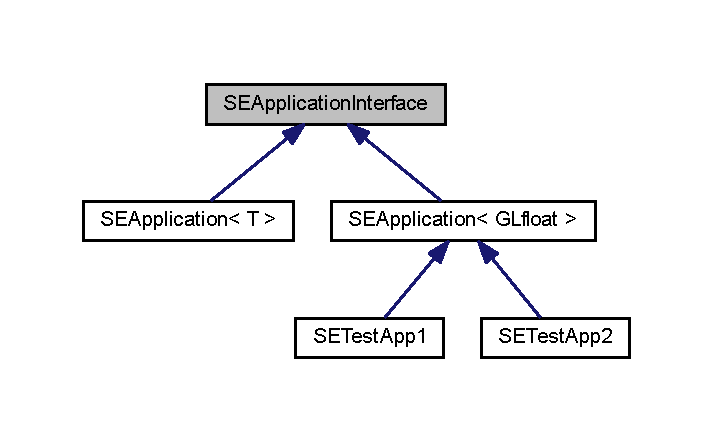
\includegraphics[width=342pt]{class_s_e_application_interface__inherit__graph}
\end{center}
\end{figure}
\subsection*{Public Member Functions}
\begin{DoxyCompactItemize}
\item 
virtual void {\bf init} (int argc, char $\ast$$\ast$argv)=0
\item 
virtual void {\bf run} ()=0
\item 
virtual void {\bf update} ()=0
\item 
virtual void {\bf quit} ()=0
\item 
virtual void {\bf pause} ()
\item 
virtual {\bf S\+E\+Window\+Manager} $\ast$ {\bf wm} ()=0
\item 
virtual {\bf S\+E\+Flow\+Controller} $\ast$ {\bf fc} ()=0
\item 
virtual {\bf S\+E\+Render\+Service} $\ast$ {\bf rs} ()=0
\item 
virtual void {\bf reshape} (int width, int height)
\item 
virtual void {\bf display} ()=0
\item 
virtual void {\bf key} (unsigned char key, int x, int y)
\item 
virtual void {\bf press\+Func\+Key} (int {\bf key}, int x1, int y1)
\item 
virtual void {\bf release\+Func\+Key} (int {\bf key}, int x, int y)
\item 
virtual void {\bf mouse\+Motion} (int x, int y)
\item 
virtual void {\bf mouse\+Passive\+Motion} (int x, int y)
\item 
virtual void {\bf mouse\+Button} (int button, int state, int x, int y)
\item 
virtual void {\bf idle} ()
\item 
{\bf $\sim$\+S\+E\+Application\+Interface} ()
\end{DoxyCompactItemize}
\subsection*{Public Attributes}
\begin{DoxyCompactItemize}
\item 
const bool \& {\bf is\+Running}
\item 
const bool \& {\bf is\+Updating}
\end{DoxyCompactItemize}
\subsection*{Protected Member Functions}
\begin{DoxyCompactItemize}
\item 
{\bf S\+E\+Application\+Interface} ()
\end{DoxyCompactItemize}
\subsection*{Protected Attributes}
\begin{DoxyCompactItemize}
\item 
bool {\bf run\+\_\+}
\item 
bool {\bf update\+\_\+}
\end{DoxyCompactItemize}


\subsection{Detailed Description}


Definition at line 8 of file S\+E\+Application\+Interface.\+h.



\subsection{Constructor \& Destructor Documentation}
\index{S\+E\+Application\+Interface@{S\+E\+Application\+Interface}!````~S\+E\+Application\+Interface@{$\sim$\+S\+E\+Application\+Interface}}
\index{````~S\+E\+Application\+Interface@{$\sim$\+S\+E\+Application\+Interface}!S\+E\+Application\+Interface@{S\+E\+Application\+Interface}}
\subsubsection[{$\sim$\+S\+E\+Application\+Interface}]{\setlength{\rightskip}{0pt plus 5cm}S\+E\+Application\+Interface\+::$\sim$\+S\+E\+Application\+Interface (
\begin{DoxyParamCaption}
{}
\end{DoxyParamCaption}
)\hspace{0.3cm}{\ttfamily [inline]}}\label{class_s_e_application_interface_a892629f2d5f0b0af0b2a15138beea85e}


Definition at line 38 of file S\+E\+Application\+Interface.\+h.

\index{S\+E\+Application\+Interface@{S\+E\+Application\+Interface}!S\+E\+Application\+Interface@{S\+E\+Application\+Interface}}
\index{S\+E\+Application\+Interface@{S\+E\+Application\+Interface}!S\+E\+Application\+Interface@{S\+E\+Application\+Interface}}
\subsubsection[{S\+E\+Application\+Interface}]{\setlength{\rightskip}{0pt plus 5cm}S\+E\+Application\+Interface\+::\+S\+E\+Application\+Interface (
\begin{DoxyParamCaption}
{}
\end{DoxyParamCaption}
)\hspace{0.3cm}{\ttfamily [inline]}, {\ttfamily [protected]}}\label{class_s_e_application_interface_a6977d0e4fec3c54d9c87d0caf71b9ce4}


Definition at line 44 of file S\+E\+Application\+Interface.\+h.



\subsection{Member Function Documentation}
\index{S\+E\+Application\+Interface@{S\+E\+Application\+Interface}!display@{display}}
\index{display@{display}!S\+E\+Application\+Interface@{S\+E\+Application\+Interface}}
\subsubsection[{display}]{\setlength{\rightskip}{0pt plus 5cm}virtual void S\+E\+Application\+Interface\+::display (
\begin{DoxyParamCaption}
{}
\end{DoxyParamCaption}
)\hspace{0.3cm}{\ttfamily [pure virtual]}}\label{class_s_e_application_interface_a7dbd81ef6669b220b75a190f5ac19d2c}


Implemented in {\bf S\+E\+Application$<$ T $>$} \doxyref{}{p.}{class_s_e_application_af68fb4de72017976c14e4e81a35f509f}, {\bf S\+E\+Application$<$ G\+Lfloat $>$} \doxyref{}{p.}{class_s_e_application_af68fb4de72017976c14e4e81a35f509f}, {\bf S\+E\+Test\+App1} \doxyref{}{p.}{class_s_e_test_app1_aa673ae83a7249cd54756a4a475594c18}, and {\bf S\+E\+Test\+App2} \doxyref{}{p.}{class_s_e_test_app2_a7d4d1ed4ffec940cffaa677638439dd0}.

\index{S\+E\+Application\+Interface@{S\+E\+Application\+Interface}!fc@{fc}}
\index{fc@{fc}!S\+E\+Application\+Interface@{S\+E\+Application\+Interface}}
\subsubsection[{fc}]{\setlength{\rightskip}{0pt plus 5cm}virtual {\bf S\+E\+Flow\+Controller}$\ast$ S\+E\+Application\+Interface\+::fc (
\begin{DoxyParamCaption}
{}
\end{DoxyParamCaption}
)\hspace{0.3cm}{\ttfamily [pure virtual]}}\label{class_s_e_application_interface_aaf13d84e9c716f4fa7131f287f5e823b}


Implemented in {\bf S\+E\+Application$<$ T $>$} \doxyref{}{p.}{class_s_e_application_a8b62aedc2f6fee908272cb9b6638d87e}, and {\bf S\+E\+Application$<$ G\+Lfloat $>$} \doxyref{}{p.}{class_s_e_application_a8b62aedc2f6fee908272cb9b6638d87e}.

\index{S\+E\+Application\+Interface@{S\+E\+Application\+Interface}!idle@{idle}}
\index{idle@{idle}!S\+E\+Application\+Interface@{S\+E\+Application\+Interface}}
\subsubsection[{idle}]{\setlength{\rightskip}{0pt plus 5cm}virtual void S\+E\+Application\+Interface\+::idle (
\begin{DoxyParamCaption}
{}
\end{DoxyParamCaption}
)\hspace{0.3cm}{\ttfamily [inline]}, {\ttfamily [virtual]}}\label{class_s_e_application_interface_ace0d1433d2f5b08c9cd582318eabcffc}


Reimplemented in {\bf S\+E\+Test\+App1} \doxyref{}{p.}{class_s_e_test_app1_a2a3457e16ee71cba6aa71728ecd98045}, {\bf S\+E\+Application$<$ T $>$} \doxyref{}{p.}{class_s_e_application_ae10739b2876ad09ee15590ba822e21eb}, {\bf S\+E\+Test\+App2} \doxyref{}{p.}{class_s_e_test_app2_a08d31acfd918a2ee16bff9fec0927b6d}, and {\bf S\+E\+Application$<$ G\+Lfloat $>$} \doxyref{}{p.}{class_s_e_application_ae10739b2876ad09ee15590ba822e21eb}.



Definition at line 36 of file S\+E\+Application\+Interface.\+h.

\index{S\+E\+Application\+Interface@{S\+E\+Application\+Interface}!init@{init}}
\index{init@{init}!S\+E\+Application\+Interface@{S\+E\+Application\+Interface}}
\subsubsection[{init}]{\setlength{\rightskip}{0pt plus 5cm}virtual void S\+E\+Application\+Interface\+::init (
\begin{DoxyParamCaption}
\item[{int}]{argc, }
\item[{char $\ast$$\ast$}]{argv}
\end{DoxyParamCaption}
)\hspace{0.3cm}{\ttfamily [pure virtual]}}\label{class_s_e_application_interface_a6122d2fc9569a97ee0d69145a9a76779}


Implemented in {\bf S\+E\+Test\+App1} \doxyref{}{p.}{class_s_e_test_app1_ac03290087ff6592a7d368edea13b66c9}, {\bf S\+E\+Application$<$ T $>$} \doxyref{}{p.}{class_s_e_application_ae8453fdab08443b4a1c7fc9db1a4436e}, {\bf S\+E\+Application$<$ G\+Lfloat $>$} \doxyref{}{p.}{class_s_e_application_ae8453fdab08443b4a1c7fc9db1a4436e}, and {\bf S\+E\+Test\+App2} \doxyref{}{p.}{class_s_e_test_app2_a8b0e69df9de394aa9c21855570bb1d1d}.

\index{S\+E\+Application\+Interface@{S\+E\+Application\+Interface}!key@{key}}
\index{key@{key}!S\+E\+Application\+Interface@{S\+E\+Application\+Interface}}
\subsubsection[{key}]{\setlength{\rightskip}{0pt plus 5cm}virtual void S\+E\+Application\+Interface\+::key (
\begin{DoxyParamCaption}
\item[{unsigned char}]{key, }
\item[{int}]{x, }
\item[{int}]{y}
\end{DoxyParamCaption}
)\hspace{0.3cm}{\ttfamily [inline]}, {\ttfamily [virtual]}}\label{class_s_e_application_interface_acd5f51c154c4a2c737838ec40041be1b}


Reimplemented in {\bf S\+E\+Test\+App1} \doxyref{}{p.}{class_s_e_test_app1_a1ea803fab9cec1d81d681ab97a34a204}, and {\bf S\+E\+Test\+App2} \doxyref{}{p.}{class_s_e_test_app2_ae37b6ec52d90c1f62170f053dbf0526b}.



Definition at line 30 of file S\+E\+Application\+Interface.\+h.

\index{S\+E\+Application\+Interface@{S\+E\+Application\+Interface}!mouse\+Button@{mouse\+Button}}
\index{mouse\+Button@{mouse\+Button}!S\+E\+Application\+Interface@{S\+E\+Application\+Interface}}
\subsubsection[{mouse\+Button}]{\setlength{\rightskip}{0pt plus 5cm}virtual void S\+E\+Application\+Interface\+::mouse\+Button (
\begin{DoxyParamCaption}
\item[{int}]{button, }
\item[{int}]{state, }
\item[{int}]{x, }
\item[{int}]{y}
\end{DoxyParamCaption}
)\hspace{0.3cm}{\ttfamily [inline]}, {\ttfamily [virtual]}}\label{class_s_e_application_interface_a5db6174742c37baa211ffe4a27060937}


Reimplemented in {\bf S\+E\+Test\+App1} \doxyref{}{p.}{class_s_e_test_app1_a0efd8d821216c211238add35b154fc09}, and {\bf S\+E\+Test\+App2} \doxyref{}{p.}{class_s_e_test_app2_afb3e88e8abf580f65b108c2762b30936}.



Definition at line 35 of file S\+E\+Application\+Interface.\+h.

\index{S\+E\+Application\+Interface@{S\+E\+Application\+Interface}!mouse\+Motion@{mouse\+Motion}}
\index{mouse\+Motion@{mouse\+Motion}!S\+E\+Application\+Interface@{S\+E\+Application\+Interface}}
\subsubsection[{mouse\+Motion}]{\setlength{\rightskip}{0pt plus 5cm}virtual void S\+E\+Application\+Interface\+::mouse\+Motion (
\begin{DoxyParamCaption}
\item[{int}]{x, }
\item[{int}]{y}
\end{DoxyParamCaption}
)\hspace{0.3cm}{\ttfamily [inline]}, {\ttfamily [virtual]}}\label{class_s_e_application_interface_a6abe2c0685be65c24d8fd0465f001cf4}


Reimplemented in {\bf S\+E\+Test\+App1} \doxyref{}{p.}{class_s_e_test_app1_a149c2f4b986bbe39b45725ab93a990a6}, and {\bf S\+E\+Test\+App2} \doxyref{}{p.}{class_s_e_test_app2_ab391ca8e2a5db124410d26ed5a86f46d}.



Definition at line 33 of file S\+E\+Application\+Interface.\+h.

\index{S\+E\+Application\+Interface@{S\+E\+Application\+Interface}!mouse\+Passive\+Motion@{mouse\+Passive\+Motion}}
\index{mouse\+Passive\+Motion@{mouse\+Passive\+Motion}!S\+E\+Application\+Interface@{S\+E\+Application\+Interface}}
\subsubsection[{mouse\+Passive\+Motion}]{\setlength{\rightskip}{0pt plus 5cm}virtual void S\+E\+Application\+Interface\+::mouse\+Passive\+Motion (
\begin{DoxyParamCaption}
\item[{int}]{x, }
\item[{int}]{y}
\end{DoxyParamCaption}
)\hspace{0.3cm}{\ttfamily [inline]}, {\ttfamily [virtual]}}\label{class_s_e_application_interface_a316065494e0cbabf84dc6070b44227ae}


Reimplemented in {\bf S\+E\+Test\+App1} \doxyref{}{p.}{class_s_e_test_app1_a5c451c8fae948f7f8c712ed4c1b00fe0}, and {\bf S\+E\+Test\+App2} \doxyref{}{p.}{class_s_e_test_app2_a4f91ab6485750c71084ca9898f220ebb}.



Definition at line 34 of file S\+E\+Application\+Interface.\+h.

\index{S\+E\+Application\+Interface@{S\+E\+Application\+Interface}!pause@{pause}}
\index{pause@{pause}!S\+E\+Application\+Interface@{S\+E\+Application\+Interface}}
\subsubsection[{pause}]{\setlength{\rightskip}{0pt plus 5cm}virtual void S\+E\+Application\+Interface\+::pause (
\begin{DoxyParamCaption}
{}
\end{DoxyParamCaption}
)\hspace{0.3cm}{\ttfamily [inline]}, {\ttfamily [virtual]}}\label{class_s_e_application_interface_a922a7ff1c71d7a84f9bb8a08a8330172}


Definition at line 21 of file S\+E\+Application\+Interface.\+h.

\index{S\+E\+Application\+Interface@{S\+E\+Application\+Interface}!press\+Func\+Key@{press\+Func\+Key}}
\index{press\+Func\+Key@{press\+Func\+Key}!S\+E\+Application\+Interface@{S\+E\+Application\+Interface}}
\subsubsection[{press\+Func\+Key}]{\setlength{\rightskip}{0pt plus 5cm}virtual void S\+E\+Application\+Interface\+::press\+Func\+Key (
\begin{DoxyParamCaption}
\item[{int}]{key, }
\item[{int}]{x1, }
\item[{int}]{y1}
\end{DoxyParamCaption}
)\hspace{0.3cm}{\ttfamily [inline]}, {\ttfamily [virtual]}}\label{class_s_e_application_interface_a182ca84a624630be02901bf25acaeda1}


Reimplemented in {\bf S\+E\+Test\+App1} \doxyref{}{p.}{class_s_e_test_app1_a19ab2fcf8818c492ddc0f5de73f7c1e2}, and {\bf S\+E\+Test\+App2} \doxyref{}{p.}{class_s_e_test_app2_ae96c3b6084feea0d85591d7493f98f1b}.



Definition at line 31 of file S\+E\+Application\+Interface.\+h.

\index{S\+E\+Application\+Interface@{S\+E\+Application\+Interface}!quit@{quit}}
\index{quit@{quit}!S\+E\+Application\+Interface@{S\+E\+Application\+Interface}}
\subsubsection[{quit}]{\setlength{\rightskip}{0pt plus 5cm}virtual void S\+E\+Application\+Interface\+::quit (
\begin{DoxyParamCaption}
{}
\end{DoxyParamCaption}
)\hspace{0.3cm}{\ttfamily [pure virtual]}}\label{class_s_e_application_interface_ac1c05e2c7c83d66e6c5dbe52b2bd681b}


Implemented in {\bf S\+E\+Test\+App1} \doxyref{}{p.}{class_s_e_test_app1_adb78b0efdd9da9dc098d4ffa6828f727}, {\bf S\+E\+Application$<$ T $>$} \doxyref{}{p.}{class_s_e_application_a1d6dd2dd21b3e0ec2fb519c18be75456}, {\bf S\+E\+Application$<$ G\+Lfloat $>$} \doxyref{}{p.}{class_s_e_application_a1d6dd2dd21b3e0ec2fb519c18be75456}, and {\bf S\+E\+Test\+App2} \doxyref{}{p.}{class_s_e_test_app2_ab11859c0ab08874e228654bde04b30d6}.

\index{S\+E\+Application\+Interface@{S\+E\+Application\+Interface}!release\+Func\+Key@{release\+Func\+Key}}
\index{release\+Func\+Key@{release\+Func\+Key}!S\+E\+Application\+Interface@{S\+E\+Application\+Interface}}
\subsubsection[{release\+Func\+Key}]{\setlength{\rightskip}{0pt plus 5cm}virtual void S\+E\+Application\+Interface\+::release\+Func\+Key (
\begin{DoxyParamCaption}
\item[{int}]{key, }
\item[{int}]{x, }
\item[{int}]{y}
\end{DoxyParamCaption}
)\hspace{0.3cm}{\ttfamily [inline]}, {\ttfamily [virtual]}}\label{class_s_e_application_interface_a245cf5d5dcc59e04873a69d8b6212415}


Reimplemented in {\bf S\+E\+Test\+App1} \doxyref{}{p.}{class_s_e_test_app1_ae897393d6528b677807f66bbe5b24080}, and {\bf S\+E\+Test\+App2} \doxyref{}{p.}{class_s_e_test_app2_a764c4e683cfebe5390e1ec4e74fb97ec}.



Definition at line 32 of file S\+E\+Application\+Interface.\+h.

\index{S\+E\+Application\+Interface@{S\+E\+Application\+Interface}!reshape@{reshape}}
\index{reshape@{reshape}!S\+E\+Application\+Interface@{S\+E\+Application\+Interface}}
\subsubsection[{reshape}]{\setlength{\rightskip}{0pt plus 5cm}virtual void S\+E\+Application\+Interface\+::reshape (
\begin{DoxyParamCaption}
\item[{int}]{width, }
\item[{int}]{height}
\end{DoxyParamCaption}
)\hspace{0.3cm}{\ttfamily [inline]}, {\ttfamily [virtual]}}\label{class_s_e_application_interface_ad1569a4561e3fec8481b17e24843fb8e}


Reimplemented in {\bf S\+E\+Test\+App1} \doxyref{}{p.}{class_s_e_test_app1_a6532c55637b099cf41f7bdfae17b0fde}, and {\bf S\+E\+Test\+App2} \doxyref{}{p.}{class_s_e_test_app2_aca71876ce43d078efd52f5d33f464b50}.



Definition at line 28 of file S\+E\+Application\+Interface.\+h.

\index{S\+E\+Application\+Interface@{S\+E\+Application\+Interface}!rs@{rs}}
\index{rs@{rs}!S\+E\+Application\+Interface@{S\+E\+Application\+Interface}}
\subsubsection[{rs}]{\setlength{\rightskip}{0pt plus 5cm}virtual {\bf S\+E\+Render\+Service}$\ast$ S\+E\+Application\+Interface\+::rs (
\begin{DoxyParamCaption}
{}
\end{DoxyParamCaption}
)\hspace{0.3cm}{\ttfamily [pure virtual]}}\label{class_s_e_application_interface_a3f3ad17c66f7e5154c06a1b51c64f79b}


Implemented in {\bf S\+E\+Application$<$ T $>$} \doxyref{}{p.}{class_s_e_application_accb31e9ba20aba3b9e87fdebe890b112}, and {\bf S\+E\+Application$<$ G\+Lfloat $>$} \doxyref{}{p.}{class_s_e_application_accb31e9ba20aba3b9e87fdebe890b112}.

\index{S\+E\+Application\+Interface@{S\+E\+Application\+Interface}!run@{run}}
\index{run@{run}!S\+E\+Application\+Interface@{S\+E\+Application\+Interface}}
\subsubsection[{run}]{\setlength{\rightskip}{0pt plus 5cm}virtual void S\+E\+Application\+Interface\+::run (
\begin{DoxyParamCaption}
{}
\end{DoxyParamCaption}
)\hspace{0.3cm}{\ttfamily [pure virtual]}}\label{class_s_e_application_interface_a80314f1b5d2ee927f0aec52d2939a4e3}


Implemented in {\bf S\+E\+Test\+App1} \doxyref{}{p.}{class_s_e_test_app1_ab3f47fe7c735bc68d2e18867011d33a2}, {\bf S\+E\+Application$<$ T $>$} \doxyref{}{p.}{class_s_e_application_a1cb54d6b2e488ec96ec0bd743f73e68e}, {\bf S\+E\+Application$<$ G\+Lfloat $>$} \doxyref{}{p.}{class_s_e_application_a1cb54d6b2e488ec96ec0bd743f73e68e}, and {\bf S\+E\+Test\+App2} \doxyref{}{p.}{class_s_e_test_app2_a721c6c574531fcd0786bb8f39683dd7e}.

\index{S\+E\+Application\+Interface@{S\+E\+Application\+Interface}!update@{update}}
\index{update@{update}!S\+E\+Application\+Interface@{S\+E\+Application\+Interface}}
\subsubsection[{update}]{\setlength{\rightskip}{0pt plus 5cm}virtual void S\+E\+Application\+Interface\+::update (
\begin{DoxyParamCaption}
{}
\end{DoxyParamCaption}
)\hspace{0.3cm}{\ttfamily [pure virtual]}}\label{class_s_e_application_interface_a39015bc105f533bad135e75f4f906315}


Implemented in {\bf S\+E\+Test\+App1} \doxyref{}{p.}{class_s_e_test_app1_a86068ad6339587aff379ad4448feed19}, and {\bf S\+E\+Test\+App2} \doxyref{}{p.}{class_s_e_test_app2_ac7d93b733cdbe5532b6d106263d6027c}.

\index{S\+E\+Application\+Interface@{S\+E\+Application\+Interface}!wm@{wm}}
\index{wm@{wm}!S\+E\+Application\+Interface@{S\+E\+Application\+Interface}}
\subsubsection[{wm}]{\setlength{\rightskip}{0pt plus 5cm}virtual {\bf S\+E\+Window\+Manager}$\ast$ S\+E\+Application\+Interface\+::wm (
\begin{DoxyParamCaption}
{}
\end{DoxyParamCaption}
)\hspace{0.3cm}{\ttfamily [pure virtual]}}\label{class_s_e_application_interface_a741d9bee928dc78ea56fe6de72137393}


Implemented in {\bf S\+E\+Application$<$ T $>$} \doxyref{}{p.}{class_s_e_application_a06d1f50c567761756a3dcf30e5bddefc}, and {\bf S\+E\+Application$<$ G\+Lfloat $>$} \doxyref{}{p.}{class_s_e_application_a06d1f50c567761756a3dcf30e5bddefc}.



\subsection{Member Data Documentation}
\index{S\+E\+Application\+Interface@{S\+E\+Application\+Interface}!is\+Running@{is\+Running}}
\index{is\+Running@{is\+Running}!S\+E\+Application\+Interface@{S\+E\+Application\+Interface}}
\subsubsection[{is\+Running}]{\setlength{\rightskip}{0pt plus 5cm}const bool\& S\+E\+Application\+Interface\+::is\+Running}\label{class_s_e_application_interface_a0adfae0ab67de7e8369087340c78d82b}


Definition at line 11 of file S\+E\+Application\+Interface.\+h.

\index{S\+E\+Application\+Interface@{S\+E\+Application\+Interface}!is\+Updating@{is\+Updating}}
\index{is\+Updating@{is\+Updating}!S\+E\+Application\+Interface@{S\+E\+Application\+Interface}}
\subsubsection[{is\+Updating}]{\setlength{\rightskip}{0pt plus 5cm}const bool\& S\+E\+Application\+Interface\+::is\+Updating}\label{class_s_e_application_interface_a193db1a904f3c8d4e7f835a44c8c8ba8}


Definition at line 12 of file S\+E\+Application\+Interface.\+h.

\index{S\+E\+Application\+Interface@{S\+E\+Application\+Interface}!run\+\_\+@{run\+\_\+}}
\index{run\+\_\+@{run\+\_\+}!S\+E\+Application\+Interface@{S\+E\+Application\+Interface}}
\subsubsection[{run\+\_\+}]{\setlength{\rightskip}{0pt plus 5cm}bool S\+E\+Application\+Interface\+::run\+\_\+\hspace{0.3cm}{\ttfamily [protected]}}\label{class_s_e_application_interface_aeb0e393d1549802031da663659196b33}


Definition at line 41 of file S\+E\+Application\+Interface.\+h.

\index{S\+E\+Application\+Interface@{S\+E\+Application\+Interface}!update\+\_\+@{update\+\_\+}}
\index{update\+\_\+@{update\+\_\+}!S\+E\+Application\+Interface@{S\+E\+Application\+Interface}}
\subsubsection[{update\+\_\+}]{\setlength{\rightskip}{0pt plus 5cm}bool S\+E\+Application\+Interface\+::update\+\_\+\hspace{0.3cm}{\ttfamily [protected]}}\label{class_s_e_application_interface_a0d944eb1f60a85bed360c85850da73d2}


Definition at line 42 of file S\+E\+Application\+Interface.\+h.



The documentation for this class was generated from the following file\+:\begin{DoxyCompactItemize}
\item 
{\bf S\+E\+Application\+Interface.\+h}\end{DoxyCompactItemize}

\section{S\+E\+Camera$<$ T $>$ Class Template Reference}
\label{class_s_e_camera}\index{S\+E\+Camera$<$ T $>$@{S\+E\+Camera$<$ T $>$}}


{\ttfamily \#include $<$S\+E\+Camera.\+h$>$}



Inheritance diagram for S\+E\+Camera$<$ T $>$\+:
\nopagebreak
\begin{figure}[H]
\begin{center}
\leavevmode
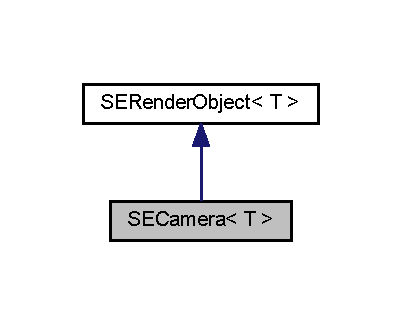
\includegraphics[width=193pt]{class_s_e_camera__inherit__graph}
\end{center}
\end{figure}


Collaboration diagram for S\+E\+Camera$<$ T $>$\+:
\nopagebreak
\begin{figure}[H]
\begin{center}
\leavevmode
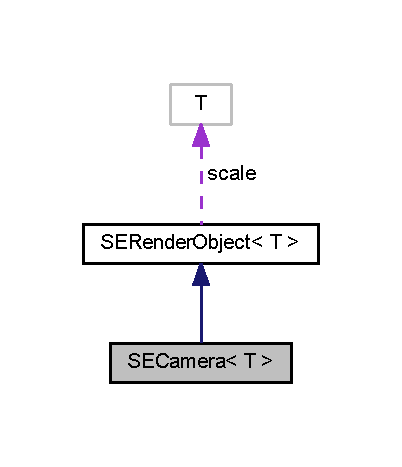
\includegraphics[width=193pt]{class_s_e_camera__coll__graph}
\end{center}
\end{figure}
\subsection*{Public Member Functions}
\begin{DoxyCompactItemize}
\item 
void {\bf use\+Ortho\+Projection} ()
\item 
void {\bf use\+Perspective\+Projection} ()
\item 
{\bf S\+E\+Camera}$<$ T $>$ \& {\bf translate\+Relative\+By} (T x, T y, T z)
\item 
{\bf S\+E\+Camera}$<$ T $>$ \& {\bf translate\+Relative\+By} (const {\bf S\+E\+Vec3}$<$ T $>$ \&t)
\item 
{\bf S\+E\+Camera}$<$ T $>$ \& {\bf translate\+Relative\+By} (const {\bf S\+E\+Vec4}$<$ T $>$ \&t)
\item 
{\bf S\+E\+Camera}$<$ T $>$ \& {\bf pan} (T r)
\item 
{\bf S\+E\+Camera}$<$ T $>$ \& {\bf pan\+Left} (T r)
\item 
{\bf S\+E\+Camera}$<$ T $>$ \& {\bf pan\+Right} (T r)
\item 
{\bf S\+E\+Camera}$<$ T $>$ \& {\bf pan\+By\+Degrees} (T d)
\item 
{\bf S\+E\+Camera}$<$ T $>$ \& {\bf pan\+Left\+By\+Degrees} (T d)
\item 
{\bf S\+E\+Camera}$<$ T $>$ \& {\bf pan\+Right\+By\+Degrees} (T d)
\item 
{\bf S\+E\+Camera}$<$ T $>$ \& {\bf tilt} (T r)
\item 
{\bf S\+E\+Camera}$<$ T $>$ \& {\bf tilt\+Up} (T r)
\item 
{\bf S\+E\+Camera}$<$ T $>$ \& {\bf tilt\+Down} (T r)
\item 
{\bf S\+E\+Camera}$<$ T $>$ \& {\bf tilt\+By\+Degrees} (T d)
\item 
{\bf S\+E\+Camera}$<$ T $>$ \& {\bf tilt\+Up\+By\+Degrees} (T d)
\item 
{\bf S\+E\+Camera}$<$ T $>$ \& {\bf tilt\+Down\+By\+Degrees} (T d)
\item 
{\bf S\+E\+Camera}$<$ T $>$ \& {\bf zoom} (T z)
\item 
{\bf S\+E\+Camera}$<$ T $>$ \& {\bf zoom\+In} (T z)
\item 
{\bf S\+E\+Camera}$<$ T $>$ \& {\bf zoom\+Out} (T z)
\item 
{\bf S\+E\+Camera}$<$ T $>$ \& {\bf pedestal} (T d)
\item 
{\bf S\+E\+Camera}$<$ T $>$ \& {\bf pedestal\+Up} (T d)
\item 
{\bf S\+E\+Camera}$<$ T $>$ \& {\bf pedestal\+Down} (T d)
\item 
{\bf S\+E\+Camera}$<$ T $>$ \& {\bf dolly} (T d)
\item 
{\bf S\+E\+Camera}$<$ T $>$ \& {\bf dolly\+Front} (T d)
\item 
{\bf S\+E\+Camera}$<$ T $>$ \& {\bf dolly\+Back} (T d)
\item 
{\bf S\+E\+Camera}$<$ T $>$ \& {\bf truck} (T d)
\item 
{\bf S\+E\+Camera}$<$ T $>$ \& {\bf truck\+Right} (T d)
\item 
{\bf S\+E\+Camera}$<$ T $>$ \& {\bf truck\+Left} (T d)
\item 
virtual void {\bf render} (const {\bf S\+E\+Render\+Service\+Internals}$<$ T $>$ \&rs) const 
\item 
virtual void {\bf setup\+Frame} () const =0
\end{DoxyCompactItemize}
\subsection*{Public Attributes}
\begin{DoxyCompactItemize}
\item 
const {\bf S\+E\+Mat4}$<$ T $>$ \& {\bf projection}
\item 
const {\bf S\+E\+Frustum\+Type\+::t\+Frustum} \& {\bf frustum\+Type}
\item 
const {\bf S\+E\+Camera\+Type\+::t\+Camera} \& {\bf cam\+Type}
\end{DoxyCompactItemize}
\subsection*{Protected Member Functions}
\begin{DoxyCompactItemize}
\item 
{\bf S\+E\+Camera} ()
\item 
{\bf S\+E\+Camera} ({\bf S\+E\+Camera\+Type\+::t\+Camera} t)
\item 
virtual {\bf $\sim$\+S\+E\+Camera} ()
\end{DoxyCompactItemize}


\subsection{Detailed Description}
\subsubsection*{template$<$class T$>$class S\+E\+Camera$<$ T $>$}



Definition at line 18 of file S\+E\+Camera.\+h.



\subsection{Constructor \& Destructor Documentation}
\index{S\+E\+Camera@{S\+E\+Camera}!S\+E\+Camera@{S\+E\+Camera}}
\index{S\+E\+Camera@{S\+E\+Camera}!S\+E\+Camera@{S\+E\+Camera}}
\subsubsection[{S\+E\+Camera}]{\setlength{\rightskip}{0pt plus 5cm}template$<$class T$>$ {\bf S\+E\+Camera}$<$ T $>$\+::{\bf S\+E\+Camera} (
\begin{DoxyParamCaption}
{}
\end{DoxyParamCaption}
)\hspace{0.3cm}{\ttfamily [inline]}, {\ttfamily [protected]}}\label{class_s_e_camera_adf5bcad8576b8bbf0ce07aa0239d8dd8}


Definition at line 69 of file S\+E\+Camera.\+h.

\index{S\+E\+Camera@{S\+E\+Camera}!S\+E\+Camera@{S\+E\+Camera}}
\index{S\+E\+Camera@{S\+E\+Camera}!S\+E\+Camera@{S\+E\+Camera}}
\subsubsection[{S\+E\+Camera}]{\setlength{\rightskip}{0pt plus 5cm}template$<$class T$>$ {\bf S\+E\+Camera}$<$ T $>$\+::{\bf S\+E\+Camera} (
\begin{DoxyParamCaption}
\item[{{\bf S\+E\+Camera\+Type\+::t\+Camera}}]{t}
\end{DoxyParamCaption}
)\hspace{0.3cm}{\ttfamily [inline]}, {\ttfamily [protected]}}\label{class_s_e_camera_a84ec1e8592318ffc13b09f834c328ef6}


Definition at line 72 of file S\+E\+Camera.\+h.

\index{S\+E\+Camera@{S\+E\+Camera}!````~S\+E\+Camera@{$\sim$\+S\+E\+Camera}}
\index{````~S\+E\+Camera@{$\sim$\+S\+E\+Camera}!S\+E\+Camera@{S\+E\+Camera}}
\subsubsection[{$\sim$\+S\+E\+Camera}]{\setlength{\rightskip}{0pt plus 5cm}template$<$class T$>$ virtual {\bf S\+E\+Camera}$<$ T $>$\+::$\sim${\bf S\+E\+Camera} (
\begin{DoxyParamCaption}
{}
\end{DoxyParamCaption}
)\hspace{0.3cm}{\ttfamily [inline]}, {\ttfamily [protected]}, {\ttfamily [virtual]}}\label{class_s_e_camera_ac4da47c6fe3ba9504ce3ae0856ce33dd}


Definition at line 75 of file S\+E\+Camera.\+h.



\subsection{Member Function Documentation}
\index{S\+E\+Camera@{S\+E\+Camera}!dolly@{dolly}}
\index{dolly@{dolly}!S\+E\+Camera@{S\+E\+Camera}}
\subsubsection[{dolly}]{\setlength{\rightskip}{0pt plus 5cm}template$<$class T$>$ {\bf S\+E\+Camera}$<$T$>$\& {\bf S\+E\+Camera}$<$ T $>$\+::dolly (
\begin{DoxyParamCaption}
\item[{T}]{d}
\end{DoxyParamCaption}
)\hspace{0.3cm}{\ttfamily [inline]}}\label{class_s_e_camera_af0a5c2597ecfaea3d455b442a0c76df0}


Definition at line 56 of file S\+E\+Camera.\+h.

\index{S\+E\+Camera@{S\+E\+Camera}!dolly\+Back@{dolly\+Back}}
\index{dolly\+Back@{dolly\+Back}!S\+E\+Camera@{S\+E\+Camera}}
\subsubsection[{dolly\+Back}]{\setlength{\rightskip}{0pt plus 5cm}template$<$class T$>$ {\bf S\+E\+Camera}$<$T$>$\& {\bf S\+E\+Camera}$<$ T $>$\+::dolly\+Back (
\begin{DoxyParamCaption}
\item[{T}]{d}
\end{DoxyParamCaption}
)\hspace{0.3cm}{\ttfamily [inline]}}\label{class_s_e_camera_a33edd2911059fe6e3f75d347117340e6}


Definition at line 58 of file S\+E\+Camera.\+h.

\index{S\+E\+Camera@{S\+E\+Camera}!dolly\+Front@{dolly\+Front}}
\index{dolly\+Front@{dolly\+Front}!S\+E\+Camera@{S\+E\+Camera}}
\subsubsection[{dolly\+Front}]{\setlength{\rightskip}{0pt plus 5cm}template$<$class T$>$ {\bf S\+E\+Camera}$<$T$>$\& {\bf S\+E\+Camera}$<$ T $>$\+::dolly\+Front (
\begin{DoxyParamCaption}
\item[{T}]{d}
\end{DoxyParamCaption}
)\hspace{0.3cm}{\ttfamily [inline]}}\label{class_s_e_camera_a7c57cd3b990b002b166be69e38adb7aa}


Definition at line 57 of file S\+E\+Camera.\+h.

\index{S\+E\+Camera@{S\+E\+Camera}!pan@{pan}}
\index{pan@{pan}!S\+E\+Camera@{S\+E\+Camera}}
\subsubsection[{pan}]{\setlength{\rightskip}{0pt plus 5cm}template$<$class T$>$ {\bf S\+E\+Camera}$<$T$>$\& {\bf S\+E\+Camera}$<$ T $>$\+::pan (
\begin{DoxyParamCaption}
\item[{T}]{r}
\end{DoxyParamCaption}
)\hspace{0.3cm}{\ttfamily [inline]}}\label{class_s_e_camera_ae2a93cf5c38256be12d176df9a4f2733}


Definition at line 32 of file S\+E\+Camera.\+h.

\index{S\+E\+Camera@{S\+E\+Camera}!pan\+By\+Degrees@{pan\+By\+Degrees}}
\index{pan\+By\+Degrees@{pan\+By\+Degrees}!S\+E\+Camera@{S\+E\+Camera}}
\subsubsection[{pan\+By\+Degrees}]{\setlength{\rightskip}{0pt plus 5cm}template$<$class T$>$ {\bf S\+E\+Camera}$<$T$>$\& {\bf S\+E\+Camera}$<$ T $>$\+::pan\+By\+Degrees (
\begin{DoxyParamCaption}
\item[{T}]{d}
\end{DoxyParamCaption}
)\hspace{0.3cm}{\ttfamily [inline]}}\label{class_s_e_camera_a7e9371f0cb4b46278baba153d0f48d69}


Definition at line 36 of file S\+E\+Camera.\+h.

\index{S\+E\+Camera@{S\+E\+Camera}!pan\+Left@{pan\+Left}}
\index{pan\+Left@{pan\+Left}!S\+E\+Camera@{S\+E\+Camera}}
\subsubsection[{pan\+Left}]{\setlength{\rightskip}{0pt plus 5cm}template$<$class T$>$ {\bf S\+E\+Camera}$<$T$>$\& {\bf S\+E\+Camera}$<$ T $>$\+::pan\+Left (
\begin{DoxyParamCaption}
\item[{T}]{r}
\end{DoxyParamCaption}
)\hspace{0.3cm}{\ttfamily [inline]}}\label{class_s_e_camera_af079c33268269b2ea822811fc26b61d8}


Definition at line 33 of file S\+E\+Camera.\+h.

\index{S\+E\+Camera@{S\+E\+Camera}!pan\+Left\+By\+Degrees@{pan\+Left\+By\+Degrees}}
\index{pan\+Left\+By\+Degrees@{pan\+Left\+By\+Degrees}!S\+E\+Camera@{S\+E\+Camera}}
\subsubsection[{pan\+Left\+By\+Degrees}]{\setlength{\rightskip}{0pt plus 5cm}template$<$class T$>$ {\bf S\+E\+Camera}$<$T$>$\& {\bf S\+E\+Camera}$<$ T $>$\+::pan\+Left\+By\+Degrees (
\begin{DoxyParamCaption}
\item[{T}]{d}
\end{DoxyParamCaption}
)\hspace{0.3cm}{\ttfamily [inline]}}\label{class_s_e_camera_a17ff63333b782c4e22f47438037ba135}


Definition at line 37 of file S\+E\+Camera.\+h.

\index{S\+E\+Camera@{S\+E\+Camera}!pan\+Right@{pan\+Right}}
\index{pan\+Right@{pan\+Right}!S\+E\+Camera@{S\+E\+Camera}}
\subsubsection[{pan\+Right}]{\setlength{\rightskip}{0pt plus 5cm}template$<$class T$>$ {\bf S\+E\+Camera}$<$T$>$\& {\bf S\+E\+Camera}$<$ T $>$\+::pan\+Right (
\begin{DoxyParamCaption}
\item[{T}]{r}
\end{DoxyParamCaption}
)\hspace{0.3cm}{\ttfamily [inline]}}\label{class_s_e_camera_a46d72242a9e69d5d2ee199a7ccee89d6}


Definition at line 34 of file S\+E\+Camera.\+h.

\index{S\+E\+Camera@{S\+E\+Camera}!pan\+Right\+By\+Degrees@{pan\+Right\+By\+Degrees}}
\index{pan\+Right\+By\+Degrees@{pan\+Right\+By\+Degrees}!S\+E\+Camera@{S\+E\+Camera}}
\subsubsection[{pan\+Right\+By\+Degrees}]{\setlength{\rightskip}{0pt plus 5cm}template$<$class T$>$ {\bf S\+E\+Camera}$<$T$>$\& {\bf S\+E\+Camera}$<$ T $>$\+::pan\+Right\+By\+Degrees (
\begin{DoxyParamCaption}
\item[{T}]{d}
\end{DoxyParamCaption}
)\hspace{0.3cm}{\ttfamily [inline]}}\label{class_s_e_camera_afb4e0340e180d70b2c0ed1074f127c02}


Definition at line 38 of file S\+E\+Camera.\+h.

\index{S\+E\+Camera@{S\+E\+Camera}!pedestal@{pedestal}}
\index{pedestal@{pedestal}!S\+E\+Camera@{S\+E\+Camera}}
\subsubsection[{pedestal}]{\setlength{\rightskip}{0pt plus 5cm}template$<$class T$>$ {\bf S\+E\+Camera}$<$T$>$\& {\bf S\+E\+Camera}$<$ T $>$\+::pedestal (
\begin{DoxyParamCaption}
\item[{T}]{d}
\end{DoxyParamCaption}
)\hspace{0.3cm}{\ttfamily [inline]}}\label{class_s_e_camera_a71a4e10e74dea14268b1f71f4a63d873}


Definition at line 52 of file S\+E\+Camera.\+h.

\index{S\+E\+Camera@{S\+E\+Camera}!pedestal\+Down@{pedestal\+Down}}
\index{pedestal\+Down@{pedestal\+Down}!S\+E\+Camera@{S\+E\+Camera}}
\subsubsection[{pedestal\+Down}]{\setlength{\rightskip}{0pt plus 5cm}template$<$class T$>$ {\bf S\+E\+Camera}$<$T$>$\& {\bf S\+E\+Camera}$<$ T $>$\+::pedestal\+Down (
\begin{DoxyParamCaption}
\item[{T}]{d}
\end{DoxyParamCaption}
)\hspace{0.3cm}{\ttfamily [inline]}}\label{class_s_e_camera_a70c4df3e7a8aa22d3876496a2c86bb94}


Definition at line 54 of file S\+E\+Camera.\+h.

\index{S\+E\+Camera@{S\+E\+Camera}!pedestal\+Up@{pedestal\+Up}}
\index{pedestal\+Up@{pedestal\+Up}!S\+E\+Camera@{S\+E\+Camera}}
\subsubsection[{pedestal\+Up}]{\setlength{\rightskip}{0pt plus 5cm}template$<$class T$>$ {\bf S\+E\+Camera}$<$T$>$\& {\bf S\+E\+Camera}$<$ T $>$\+::pedestal\+Up (
\begin{DoxyParamCaption}
\item[{T}]{d}
\end{DoxyParamCaption}
)\hspace{0.3cm}{\ttfamily [inline]}}\label{class_s_e_camera_ae60d089b7d74c4576ea84ad4524f9d46}


Definition at line 53 of file S\+E\+Camera.\+h.

\index{S\+E\+Camera@{S\+E\+Camera}!render@{render}}
\index{render@{render}!S\+E\+Camera@{S\+E\+Camera}}
\subsubsection[{render}]{\setlength{\rightskip}{0pt plus 5cm}template$<$class T$>$ virtual void {\bf S\+E\+Camera}$<$ T $>$\+::render (
\begin{DoxyParamCaption}
\item[{const {\bf S\+E\+Render\+Service\+Internals}$<$ T $>$ \&}]{rs}
\end{DoxyParamCaption}
) const\hspace{0.3cm}{\ttfamily [inline]}, {\ttfamily [virtual]}}\label{class_s_e_camera_a123079b771f3d33719f3978ea0c28e37}


Reimplemented from {\bf S\+E\+Render\+Object$<$ T $>$} \doxyref{}{p.}{class_s_e_render_object_a1b06ec6905e7a98ebce4b8e72d82753c}.



Definition at line 64 of file S\+E\+Camera.\+h.

\index{S\+E\+Camera@{S\+E\+Camera}!setup\+Frame@{setup\+Frame}}
\index{setup\+Frame@{setup\+Frame}!S\+E\+Camera@{S\+E\+Camera}}
\subsubsection[{setup\+Frame}]{\setlength{\rightskip}{0pt plus 5cm}template$<$class T$>$ virtual void {\bf S\+E\+Camera}$<$ T $>$\+::setup\+Frame (
\begin{DoxyParamCaption}
{}
\end{DoxyParamCaption}
) const\hspace{0.3cm}{\ttfamily [pure virtual]}}\label{class_s_e_camera_a0c7f974b68ab4539606335d3711d4119}


Implemented in {\bf S\+E\+Open\+G\+L\+Camera} \doxyref{}{p.}{class_s_e_open_g_l_camera_a57a43f4e3f13fd2221c035c95b1134a5}.

\index{S\+E\+Camera@{S\+E\+Camera}!tilt@{tilt}}
\index{tilt@{tilt}!S\+E\+Camera@{S\+E\+Camera}}
\subsubsection[{tilt}]{\setlength{\rightskip}{0pt plus 5cm}template$<$class T$>$ {\bf S\+E\+Camera}$<$T$>$\& {\bf S\+E\+Camera}$<$ T $>$\+::tilt (
\begin{DoxyParamCaption}
\item[{T}]{r}
\end{DoxyParamCaption}
)\hspace{0.3cm}{\ttfamily [inline]}}\label{class_s_e_camera_a0d79f28e0ee97886edf6e1b610642726}


Definition at line 40 of file S\+E\+Camera.\+h.

\index{S\+E\+Camera@{S\+E\+Camera}!tilt\+By\+Degrees@{tilt\+By\+Degrees}}
\index{tilt\+By\+Degrees@{tilt\+By\+Degrees}!S\+E\+Camera@{S\+E\+Camera}}
\subsubsection[{tilt\+By\+Degrees}]{\setlength{\rightskip}{0pt plus 5cm}template$<$class T$>$ {\bf S\+E\+Camera}$<$T$>$\& {\bf S\+E\+Camera}$<$ T $>$\+::tilt\+By\+Degrees (
\begin{DoxyParamCaption}
\item[{T}]{d}
\end{DoxyParamCaption}
)\hspace{0.3cm}{\ttfamily [inline]}}\label{class_s_e_camera_a9e59da58a03159a411ecd824ac329cff}


Definition at line 44 of file S\+E\+Camera.\+h.

\index{S\+E\+Camera@{S\+E\+Camera}!tilt\+Down@{tilt\+Down}}
\index{tilt\+Down@{tilt\+Down}!S\+E\+Camera@{S\+E\+Camera}}
\subsubsection[{tilt\+Down}]{\setlength{\rightskip}{0pt plus 5cm}template$<$class T$>$ {\bf S\+E\+Camera}$<$T$>$\& {\bf S\+E\+Camera}$<$ T $>$\+::tilt\+Down (
\begin{DoxyParamCaption}
\item[{T}]{r}
\end{DoxyParamCaption}
)\hspace{0.3cm}{\ttfamily [inline]}}\label{class_s_e_camera_a3437a9f6decf17e96271540fb751ff6c}


Definition at line 42 of file S\+E\+Camera.\+h.

\index{S\+E\+Camera@{S\+E\+Camera}!tilt\+Down\+By\+Degrees@{tilt\+Down\+By\+Degrees}}
\index{tilt\+Down\+By\+Degrees@{tilt\+Down\+By\+Degrees}!S\+E\+Camera@{S\+E\+Camera}}
\subsubsection[{tilt\+Down\+By\+Degrees}]{\setlength{\rightskip}{0pt plus 5cm}template$<$class T$>$ {\bf S\+E\+Camera}$<$T$>$\& {\bf S\+E\+Camera}$<$ T $>$\+::tilt\+Down\+By\+Degrees (
\begin{DoxyParamCaption}
\item[{T}]{d}
\end{DoxyParamCaption}
)\hspace{0.3cm}{\ttfamily [inline]}}\label{class_s_e_camera_a5574590e84c1929dcccdbfa0a86563a3}


Definition at line 46 of file S\+E\+Camera.\+h.

\index{S\+E\+Camera@{S\+E\+Camera}!tilt\+Up@{tilt\+Up}}
\index{tilt\+Up@{tilt\+Up}!S\+E\+Camera@{S\+E\+Camera}}
\subsubsection[{tilt\+Up}]{\setlength{\rightskip}{0pt plus 5cm}template$<$class T$>$ {\bf S\+E\+Camera}$<$T$>$\& {\bf S\+E\+Camera}$<$ T $>$\+::tilt\+Up (
\begin{DoxyParamCaption}
\item[{T}]{r}
\end{DoxyParamCaption}
)\hspace{0.3cm}{\ttfamily [inline]}}\label{class_s_e_camera_afea54602000f2e6686dfcfe80a608a1e}


Definition at line 41 of file S\+E\+Camera.\+h.

\index{S\+E\+Camera@{S\+E\+Camera}!tilt\+Up\+By\+Degrees@{tilt\+Up\+By\+Degrees}}
\index{tilt\+Up\+By\+Degrees@{tilt\+Up\+By\+Degrees}!S\+E\+Camera@{S\+E\+Camera}}
\subsubsection[{tilt\+Up\+By\+Degrees}]{\setlength{\rightskip}{0pt plus 5cm}template$<$class T$>$ {\bf S\+E\+Camera}$<$T$>$\& {\bf S\+E\+Camera}$<$ T $>$\+::tilt\+Up\+By\+Degrees (
\begin{DoxyParamCaption}
\item[{T}]{d}
\end{DoxyParamCaption}
)\hspace{0.3cm}{\ttfamily [inline]}}\label{class_s_e_camera_ad65a11254088fbd8e92bf98240456d9b}


Definition at line 45 of file S\+E\+Camera.\+h.

\index{S\+E\+Camera@{S\+E\+Camera}!translate\+Relative\+By@{translate\+Relative\+By}}
\index{translate\+Relative\+By@{translate\+Relative\+By}!S\+E\+Camera@{S\+E\+Camera}}
\subsubsection[{translate\+Relative\+By}]{\setlength{\rightskip}{0pt plus 5cm}template$<$class T$>$ {\bf S\+E\+Camera}$<$T$>$\& {\bf S\+E\+Camera}$<$ T $>$\+::translate\+Relative\+By (
\begin{DoxyParamCaption}
\item[{T}]{x, }
\item[{T}]{y, }
\item[{T}]{z}
\end{DoxyParamCaption}
)\hspace{0.3cm}{\ttfamily [inline]}}\label{class_s_e_camera_adc05c447f7fac39693395eaa38443724}


Definition at line 28 of file S\+E\+Camera.\+h.

\index{S\+E\+Camera@{S\+E\+Camera}!translate\+Relative\+By@{translate\+Relative\+By}}
\index{translate\+Relative\+By@{translate\+Relative\+By}!S\+E\+Camera@{S\+E\+Camera}}
\subsubsection[{translate\+Relative\+By}]{\setlength{\rightskip}{0pt plus 5cm}template$<$class T$>$ {\bf S\+E\+Camera}$<$T$>$\& {\bf S\+E\+Camera}$<$ T $>$\+::translate\+Relative\+By (
\begin{DoxyParamCaption}
\item[{const {\bf S\+E\+Vec3}$<$ T $>$ \&}]{t}
\end{DoxyParamCaption}
)\hspace{0.3cm}{\ttfamily [inline]}}\label{class_s_e_camera_a55b279e301492ed96cf69940ac6c646f}


Definition at line 29 of file S\+E\+Camera.\+h.

\index{S\+E\+Camera@{S\+E\+Camera}!translate\+Relative\+By@{translate\+Relative\+By}}
\index{translate\+Relative\+By@{translate\+Relative\+By}!S\+E\+Camera@{S\+E\+Camera}}
\subsubsection[{translate\+Relative\+By}]{\setlength{\rightskip}{0pt plus 5cm}template$<$class T$>$ {\bf S\+E\+Camera}$<$T$>$\& {\bf S\+E\+Camera}$<$ T $>$\+::translate\+Relative\+By (
\begin{DoxyParamCaption}
\item[{const {\bf S\+E\+Vec4}$<$ T $>$ \&}]{t}
\end{DoxyParamCaption}
)\hspace{0.3cm}{\ttfamily [inline]}}\label{class_s_e_camera_a617d325cca358ccf17f452f714070cbc}


Definition at line 30 of file S\+E\+Camera.\+h.

\index{S\+E\+Camera@{S\+E\+Camera}!truck@{truck}}
\index{truck@{truck}!S\+E\+Camera@{S\+E\+Camera}}
\subsubsection[{truck}]{\setlength{\rightskip}{0pt plus 5cm}template$<$class T$>$ {\bf S\+E\+Camera}$<$T$>$\& {\bf S\+E\+Camera}$<$ T $>$\+::truck (
\begin{DoxyParamCaption}
\item[{T}]{d}
\end{DoxyParamCaption}
)\hspace{0.3cm}{\ttfamily [inline]}}\label{class_s_e_camera_a81415f261faf3828543a850740b12138}


Definition at line 60 of file S\+E\+Camera.\+h.

\index{S\+E\+Camera@{S\+E\+Camera}!truck\+Left@{truck\+Left}}
\index{truck\+Left@{truck\+Left}!S\+E\+Camera@{S\+E\+Camera}}
\subsubsection[{truck\+Left}]{\setlength{\rightskip}{0pt plus 5cm}template$<$class T$>$ {\bf S\+E\+Camera}$<$T$>$\& {\bf S\+E\+Camera}$<$ T $>$\+::truck\+Left (
\begin{DoxyParamCaption}
\item[{T}]{d}
\end{DoxyParamCaption}
)\hspace{0.3cm}{\ttfamily [inline]}}\label{class_s_e_camera_af68354f73d08ea2b163efdcfe647559e}


Definition at line 62 of file S\+E\+Camera.\+h.

\index{S\+E\+Camera@{S\+E\+Camera}!truck\+Right@{truck\+Right}}
\index{truck\+Right@{truck\+Right}!S\+E\+Camera@{S\+E\+Camera}}
\subsubsection[{truck\+Right}]{\setlength{\rightskip}{0pt plus 5cm}template$<$class T$>$ {\bf S\+E\+Camera}$<$T$>$\& {\bf S\+E\+Camera}$<$ T $>$\+::truck\+Right (
\begin{DoxyParamCaption}
\item[{T}]{d}
\end{DoxyParamCaption}
)\hspace{0.3cm}{\ttfamily [inline]}}\label{class_s_e_camera_a9189eb287379ab3b1992b0cbe9639051}


Definition at line 61 of file S\+E\+Camera.\+h.

\index{S\+E\+Camera@{S\+E\+Camera}!use\+Ortho\+Projection@{use\+Ortho\+Projection}}
\index{use\+Ortho\+Projection@{use\+Ortho\+Projection}!S\+E\+Camera@{S\+E\+Camera}}
\subsubsection[{use\+Ortho\+Projection}]{\setlength{\rightskip}{0pt plus 5cm}template$<$class T$>$ void {\bf S\+E\+Camera}$<$ T $>$\+::use\+Ortho\+Projection (
\begin{DoxyParamCaption}
{}
\end{DoxyParamCaption}
)\hspace{0.3cm}{\ttfamily [inline]}}\label{class_s_e_camera_aaebea4fbfae9a871aa4bda0dc96a5196}


Definition at line 25 of file S\+E\+Camera.\+h.

\index{S\+E\+Camera@{S\+E\+Camera}!use\+Perspective\+Projection@{use\+Perspective\+Projection}}
\index{use\+Perspective\+Projection@{use\+Perspective\+Projection}!S\+E\+Camera@{S\+E\+Camera}}
\subsubsection[{use\+Perspective\+Projection}]{\setlength{\rightskip}{0pt plus 5cm}template$<$class T$>$ void {\bf S\+E\+Camera}$<$ T $>$\+::use\+Perspective\+Projection (
\begin{DoxyParamCaption}
{}
\end{DoxyParamCaption}
)\hspace{0.3cm}{\ttfamily [inline]}}\label{class_s_e_camera_a847b4f245e824522fbd7a241b257372d}


Definition at line 26 of file S\+E\+Camera.\+h.

\index{S\+E\+Camera@{S\+E\+Camera}!zoom@{zoom}}
\index{zoom@{zoom}!S\+E\+Camera@{S\+E\+Camera}}
\subsubsection[{zoom}]{\setlength{\rightskip}{0pt plus 5cm}template$<$class T$>$ {\bf S\+E\+Camera}$<$T$>$\& {\bf S\+E\+Camera}$<$ T $>$\+::zoom (
\begin{DoxyParamCaption}
\item[{T}]{z}
\end{DoxyParamCaption}
)\hspace{0.3cm}{\ttfamily [inline]}}\label{class_s_e_camera_ad9e1e3ca9c13fd2592b66733287e7218}


Definition at line 48 of file S\+E\+Camera.\+h.

\index{S\+E\+Camera@{S\+E\+Camera}!zoom\+In@{zoom\+In}}
\index{zoom\+In@{zoom\+In}!S\+E\+Camera@{S\+E\+Camera}}
\subsubsection[{zoom\+In}]{\setlength{\rightskip}{0pt plus 5cm}template$<$class T$>$ {\bf S\+E\+Camera}$<$T$>$\& {\bf S\+E\+Camera}$<$ T $>$\+::zoom\+In (
\begin{DoxyParamCaption}
\item[{T}]{z}
\end{DoxyParamCaption}
)\hspace{0.3cm}{\ttfamily [inline]}}\label{class_s_e_camera_abc697be1b628b78c985908ed0238001f}


Definition at line 49 of file S\+E\+Camera.\+h.

\index{S\+E\+Camera@{S\+E\+Camera}!zoom\+Out@{zoom\+Out}}
\index{zoom\+Out@{zoom\+Out}!S\+E\+Camera@{S\+E\+Camera}}
\subsubsection[{zoom\+Out}]{\setlength{\rightskip}{0pt plus 5cm}template$<$class T$>$ {\bf S\+E\+Camera}$<$T$>$\& {\bf S\+E\+Camera}$<$ T $>$\+::zoom\+Out (
\begin{DoxyParamCaption}
\item[{T}]{z}
\end{DoxyParamCaption}
)\hspace{0.3cm}{\ttfamily [inline]}}\label{class_s_e_camera_a5710abc3c3a09850c1e41576daf41013}


Definition at line 50 of file S\+E\+Camera.\+h.



\subsection{Member Data Documentation}
\index{S\+E\+Camera@{S\+E\+Camera}!cam\+Type@{cam\+Type}}
\index{cam\+Type@{cam\+Type}!S\+E\+Camera@{S\+E\+Camera}}
\subsubsection[{cam\+Type}]{\setlength{\rightskip}{0pt plus 5cm}template$<$class T$>$ const {\bf S\+E\+Camera\+Type\+::t\+Camera}\& {\bf S\+E\+Camera}$<$ T $>$\+::cam\+Type}\label{class_s_e_camera_a60c7bdd0250aa51e0e72e24b37a1a28d}


Definition at line 23 of file S\+E\+Camera.\+h.

\index{S\+E\+Camera@{S\+E\+Camera}!frustum\+Type@{frustum\+Type}}
\index{frustum\+Type@{frustum\+Type}!S\+E\+Camera@{S\+E\+Camera}}
\subsubsection[{frustum\+Type}]{\setlength{\rightskip}{0pt plus 5cm}template$<$class T$>$ const {\bf S\+E\+Frustum\+Type\+::t\+Frustum}\& {\bf S\+E\+Camera}$<$ T $>$\+::frustum\+Type}\label{class_s_e_camera_a707e3e1bf1d79a7fe7170cf48d2753cf}


Definition at line 22 of file S\+E\+Camera.\+h.

\index{S\+E\+Camera@{S\+E\+Camera}!projection@{projection}}
\index{projection@{projection}!S\+E\+Camera@{S\+E\+Camera}}
\subsubsection[{projection}]{\setlength{\rightskip}{0pt plus 5cm}template$<$class T$>$ const {\bf S\+E\+Mat4}$<$T$>$\& {\bf S\+E\+Camera}$<$ T $>$\+::projection}\label{class_s_e_camera_a24b3c5742e363acc871ee217b41ac010}


Definition at line 21 of file S\+E\+Camera.\+h.



The documentation for this class was generated from the following file\+:\begin{DoxyCompactItemize}
\item 
{\bf S\+E\+Camera.\+h}\end{DoxyCompactItemize}

\section{S\+E\+Camera\+Type Struct Reference}
\label{struct_s_e_camera_type}\index{S\+E\+Camera\+Type@{S\+E\+Camera\+Type}}


{\ttfamily \#include $<$S\+E\+Camera.\+h$>$}

\subsection*{Public Types}
\begin{DoxyCompactItemize}
\item 
enum {\bf t\+Camera} \{ \\*
{\bf S\+T\+A\+T\+I\+C\+\_\+\+C\+A\+M}, 
{\bf O\+R\+B\+I\+T\+\_\+\+C\+A\+M}, 
{\bf F\+O\+L\+L\+O\+W\+\_\+\+C\+A\+M}, 
{\bf T\+R\+A\+I\+L\+\_\+\+C\+A\+M}, 
\\*
{\bf F\+R\+E\+E\+\_\+\+C\+A\+M}, 
{\bf N\+U\+M\+\_\+\+C\+A\+M\+S}
 \}
\end{DoxyCompactItemize}


\subsection{Detailed Description}


Definition at line 8 of file S\+E\+Camera.\+h.



\subsection{Member Enumeration Documentation}
\index{S\+E\+Camera\+Type@{S\+E\+Camera\+Type}!t\+Camera@{t\+Camera}}
\index{t\+Camera@{t\+Camera}!S\+E\+Camera\+Type@{S\+E\+Camera\+Type}}
\subsubsection[{t\+Camera}]{\setlength{\rightskip}{0pt plus 5cm}enum {\bf S\+E\+Camera\+Type\+::t\+Camera}}\label{struct_s_e_camera_type_aca25385dae9d3f4471c2895339d37148}
\begin{Desc}
\item[Enumerator]\par
\begin{description}
\index{S\+T\+A\+T\+I\+C\+\_\+\+C\+A\+M@{S\+T\+A\+T\+I\+C\+\_\+\+C\+A\+M}!S\+E\+Camera\+Type@{S\+E\+Camera\+Type}}\index{S\+E\+Camera\+Type@{S\+E\+Camera\+Type}!S\+T\+A\+T\+I\+C\+\_\+\+C\+A\+M@{S\+T\+A\+T\+I\+C\+\_\+\+C\+A\+M}}\item[{\em 
S\+T\+A\+T\+I\+C\+\_\+\+C\+A\+M\label{struct_s_e_camera_type_aca25385dae9d3f4471c2895339d37148a93be7a894b708974359c54d02ec8da00}
}]\index{O\+R\+B\+I\+T\+\_\+\+C\+A\+M@{O\+R\+B\+I\+T\+\_\+\+C\+A\+M}!S\+E\+Camera\+Type@{S\+E\+Camera\+Type}}\index{S\+E\+Camera\+Type@{S\+E\+Camera\+Type}!O\+R\+B\+I\+T\+\_\+\+C\+A\+M@{O\+R\+B\+I\+T\+\_\+\+C\+A\+M}}\item[{\em 
O\+R\+B\+I\+T\+\_\+\+C\+A\+M\label{struct_s_e_camera_type_aca25385dae9d3f4471c2895339d37148a6ebae5c8873794784862c00536b221a0}
}]\index{F\+O\+L\+L\+O\+W\+\_\+\+C\+A\+M@{F\+O\+L\+L\+O\+W\+\_\+\+C\+A\+M}!S\+E\+Camera\+Type@{S\+E\+Camera\+Type}}\index{S\+E\+Camera\+Type@{S\+E\+Camera\+Type}!F\+O\+L\+L\+O\+W\+\_\+\+C\+A\+M@{F\+O\+L\+L\+O\+W\+\_\+\+C\+A\+M}}\item[{\em 
F\+O\+L\+L\+O\+W\+\_\+\+C\+A\+M\label{struct_s_e_camera_type_aca25385dae9d3f4471c2895339d37148a94094d11dfb64e3ffd9493d9e23bbee3}
}]\index{T\+R\+A\+I\+L\+\_\+\+C\+A\+M@{T\+R\+A\+I\+L\+\_\+\+C\+A\+M}!S\+E\+Camera\+Type@{S\+E\+Camera\+Type}}\index{S\+E\+Camera\+Type@{S\+E\+Camera\+Type}!T\+R\+A\+I\+L\+\_\+\+C\+A\+M@{T\+R\+A\+I\+L\+\_\+\+C\+A\+M}}\item[{\em 
T\+R\+A\+I\+L\+\_\+\+C\+A\+M\label{struct_s_e_camera_type_aca25385dae9d3f4471c2895339d37148a94f3a688263bc6dd5e2dd9ff348a5b42}
}]\index{F\+R\+E\+E\+\_\+\+C\+A\+M@{F\+R\+E\+E\+\_\+\+C\+A\+M}!S\+E\+Camera\+Type@{S\+E\+Camera\+Type}}\index{S\+E\+Camera\+Type@{S\+E\+Camera\+Type}!F\+R\+E\+E\+\_\+\+C\+A\+M@{F\+R\+E\+E\+\_\+\+C\+A\+M}}\item[{\em 
F\+R\+E\+E\+\_\+\+C\+A\+M\label{struct_s_e_camera_type_aca25385dae9d3f4471c2895339d37148ae467c5313c4b6ff43c7178dc7b2897eb}
}]\index{N\+U\+M\+\_\+\+C\+A\+M\+S@{N\+U\+M\+\_\+\+C\+A\+M\+S}!S\+E\+Camera\+Type@{S\+E\+Camera\+Type}}\index{S\+E\+Camera\+Type@{S\+E\+Camera\+Type}!N\+U\+M\+\_\+\+C\+A\+M\+S@{N\+U\+M\+\_\+\+C\+A\+M\+S}}\item[{\em 
N\+U\+M\+\_\+\+C\+A\+M\+S\label{struct_s_e_camera_type_aca25385dae9d3f4471c2895339d37148a38cc1b35195ab30cb9f59c1460dd7004}
}]\end{description}
\end{Desc}


Definition at line 10 of file S\+E\+Camera.\+h.



The documentation for this struct was generated from the following file\+:\begin{DoxyCompactItemize}
\item 
{\bf S\+E\+Camera.\+h}\end{DoxyCompactItemize}

\section{S\+E\+Chronometer$<$ T $>$ Class Template Reference}
\label{class_s_e_chronometer}\index{S\+E\+Chronometer$<$ T $>$@{S\+E\+Chronometer$<$ T $>$}}


{\ttfamily \#include $<$S\+E\+Math.\+h$>$}

\subsection*{Public Types}
\begin{DoxyCompactItemize}
\item 
enum {\bf t\+Chronometer\+State} \{ {\bf C\+S\+\_\+\+S\+T\+O\+P\+P\+E\+D}, 
{\bf C\+S\+\_\+\+P\+A\+U\+S\+E\+D}, 
{\bf C\+S\+\_\+\+R\+U\+N\+N\+I\+N\+G}, 
{\bf N\+U\+M\+\_\+\+C\+S\+S}
 \}
\end{DoxyCompactItemize}
\subsection*{Public Member Functions}
\begin{DoxyCompactItemize}
\item 
{\bf S\+E\+Chronometer} ()
\item 
{\bf $\sim$\+S\+E\+Chronometer} ()
\item 
void {\bf start} ()
\item 
void {\bf pause} ()
\item 
void {\bf stop} ()
\item 
void {\bf reset} ()
\item 
T {\bf read} ()
\end{DoxyCompactItemize}


\subsection{Detailed Description}
\subsubsection*{template$<$class T$>$class S\+E\+Chronometer$<$ T $>$}



Definition at line 47 of file S\+E\+Math.\+h.



\subsection{Member Enumeration Documentation}
\index{S\+E\+Chronometer@{S\+E\+Chronometer}!t\+Chronometer\+State@{t\+Chronometer\+State}}
\index{t\+Chronometer\+State@{t\+Chronometer\+State}!S\+E\+Chronometer@{S\+E\+Chronometer}}
\subsubsection[{t\+Chronometer\+State}]{\setlength{\rightskip}{0pt plus 5cm}template$<$class T $>$ enum {\bf S\+E\+Chronometer\+::t\+Chronometer\+State}}\label{class_s_e_chronometer_a2a991aa3e29ca3e3eb242d0473e976cd}
\begin{Desc}
\item[Enumerator]\par
\begin{description}
\index{C\+S\+\_\+\+S\+T\+O\+P\+P\+E\+D@{C\+S\+\_\+\+S\+T\+O\+P\+P\+E\+D}!S\+E\+Chronometer@{S\+E\+Chronometer}}\index{S\+E\+Chronometer@{S\+E\+Chronometer}!C\+S\+\_\+\+S\+T\+O\+P\+P\+E\+D@{C\+S\+\_\+\+S\+T\+O\+P\+P\+E\+D}}\item[{\em 
C\+S\+\_\+\+S\+T\+O\+P\+P\+E\+D\label{class_s_e_chronometer_a2a991aa3e29ca3e3eb242d0473e976cdac2fc9912d33810adaf912f8f12dfe691}
}]\index{C\+S\+\_\+\+P\+A\+U\+S\+E\+D@{C\+S\+\_\+\+P\+A\+U\+S\+E\+D}!S\+E\+Chronometer@{S\+E\+Chronometer}}\index{S\+E\+Chronometer@{S\+E\+Chronometer}!C\+S\+\_\+\+P\+A\+U\+S\+E\+D@{C\+S\+\_\+\+P\+A\+U\+S\+E\+D}}\item[{\em 
C\+S\+\_\+\+P\+A\+U\+S\+E\+D\label{class_s_e_chronometer_a2a991aa3e29ca3e3eb242d0473e976cda4dc19254e6f85ee0619bfcef651dc201}
}]\index{C\+S\+\_\+\+R\+U\+N\+N\+I\+N\+G@{C\+S\+\_\+\+R\+U\+N\+N\+I\+N\+G}!S\+E\+Chronometer@{S\+E\+Chronometer}}\index{S\+E\+Chronometer@{S\+E\+Chronometer}!C\+S\+\_\+\+R\+U\+N\+N\+I\+N\+G@{C\+S\+\_\+\+R\+U\+N\+N\+I\+N\+G}}\item[{\em 
C\+S\+\_\+\+R\+U\+N\+N\+I\+N\+G\label{class_s_e_chronometer_a2a991aa3e29ca3e3eb242d0473e976cda840546f48c4d2897e2d86f880f6083b1}
}]\index{N\+U\+M\+\_\+\+C\+S\+S@{N\+U\+M\+\_\+\+C\+S\+S}!S\+E\+Chronometer@{S\+E\+Chronometer}}\index{S\+E\+Chronometer@{S\+E\+Chronometer}!N\+U\+M\+\_\+\+C\+S\+S@{N\+U\+M\+\_\+\+C\+S\+S}}\item[{\em 
N\+U\+M\+\_\+\+C\+S\+S\label{class_s_e_chronometer_a2a991aa3e29ca3e3eb242d0473e976cdae844809291e69ea04f0469080969fff3}
}]\end{description}
\end{Desc}


Definition at line 1239 of file S\+E\+Math.\+h.



\subsection{Constructor \& Destructor Documentation}
\index{S\+E\+Chronometer@{S\+E\+Chronometer}!S\+E\+Chronometer@{S\+E\+Chronometer}}
\index{S\+E\+Chronometer@{S\+E\+Chronometer}!S\+E\+Chronometer@{S\+E\+Chronometer}}
\subsubsection[{S\+E\+Chronometer}]{\setlength{\rightskip}{0pt plus 5cm}template$<$class T $>$ {\bf S\+E\+Chronometer}$<$ T $>$\+::{\bf S\+E\+Chronometer} (
\begin{DoxyParamCaption}
{}
\end{DoxyParamCaption}
)\hspace{0.3cm}{\ttfamily [inline]}}\label{class_s_e_chronometer_a011be27454b637f949793713c628581b}


Definition at line 1241 of file S\+E\+Math.\+h.

\index{S\+E\+Chronometer@{S\+E\+Chronometer}!````~S\+E\+Chronometer@{$\sim$\+S\+E\+Chronometer}}
\index{````~S\+E\+Chronometer@{$\sim$\+S\+E\+Chronometer}!S\+E\+Chronometer@{S\+E\+Chronometer}}
\subsubsection[{$\sim$\+S\+E\+Chronometer}]{\setlength{\rightskip}{0pt plus 5cm}template$<$class T $>$ {\bf S\+E\+Chronometer}$<$ T $>$\+::$\sim${\bf S\+E\+Chronometer} (
\begin{DoxyParamCaption}
{}
\end{DoxyParamCaption}
)\hspace{0.3cm}{\ttfamily [inline]}}\label{class_s_e_chronometer_af583452d9ff8a858e4ca25b50ccbc203}


Definition at line 1242 of file S\+E\+Math.\+h.



\subsection{Member Function Documentation}
\index{S\+E\+Chronometer@{S\+E\+Chronometer}!pause@{pause}}
\index{pause@{pause}!S\+E\+Chronometer@{S\+E\+Chronometer}}
\subsubsection[{pause}]{\setlength{\rightskip}{0pt plus 5cm}template$<$class T $>$ void {\bf S\+E\+Chronometer}$<$ T $>$\+::pause (
\begin{DoxyParamCaption}
{}
\end{DoxyParamCaption}
)\hspace{0.3cm}{\ttfamily [inline]}}\label{class_s_e_chronometer_a3a2b3fe416fc6b220178f27d33bfd78c}


Definition at line 1249 of file S\+E\+Math.\+h.

\index{S\+E\+Chronometer@{S\+E\+Chronometer}!read@{read}}
\index{read@{read}!S\+E\+Chronometer@{S\+E\+Chronometer}}
\subsubsection[{read}]{\setlength{\rightskip}{0pt plus 5cm}template$<$class T $>$ T {\bf S\+E\+Chronometer}$<$ T $>$\+::read (
\begin{DoxyParamCaption}
{}
\end{DoxyParamCaption}
)\hspace{0.3cm}{\ttfamily [inline]}}\label{class_s_e_chronometer_a1368552c2be290268b1bcc146102dff0}


Definition at line 1259 of file S\+E\+Math.\+h.

\index{S\+E\+Chronometer@{S\+E\+Chronometer}!reset@{reset}}
\index{reset@{reset}!S\+E\+Chronometer@{S\+E\+Chronometer}}
\subsubsection[{reset}]{\setlength{\rightskip}{0pt plus 5cm}template$<$class T $>$ void {\bf S\+E\+Chronometer}$<$ T $>$\+::reset (
\begin{DoxyParamCaption}
{}
\end{DoxyParamCaption}
)\hspace{0.3cm}{\ttfamily [inline]}}\label{class_s_e_chronometer_a605bb193bd8b0d0fcbcc50a52b40d26a}


Definition at line 1257 of file S\+E\+Math.\+h.

\index{S\+E\+Chronometer@{S\+E\+Chronometer}!start@{start}}
\index{start@{start}!S\+E\+Chronometer@{S\+E\+Chronometer}}
\subsubsection[{start}]{\setlength{\rightskip}{0pt plus 5cm}template$<$class T $>$ void {\bf S\+E\+Chronometer}$<$ T $>$\+::start (
\begin{DoxyParamCaption}
{}
\end{DoxyParamCaption}
)\hspace{0.3cm}{\ttfamily [inline]}}\label{class_s_e_chronometer_af0aae87f699947725698ae1dbff9aa02}


Definition at line 1244 of file S\+E\+Math.\+h.

\index{S\+E\+Chronometer@{S\+E\+Chronometer}!stop@{stop}}
\index{stop@{stop}!S\+E\+Chronometer@{S\+E\+Chronometer}}
\subsubsection[{stop}]{\setlength{\rightskip}{0pt plus 5cm}template$<$class T $>$ void {\bf S\+E\+Chronometer}$<$ T $>$\+::stop (
\begin{DoxyParamCaption}
{}
\end{DoxyParamCaption}
)\hspace{0.3cm}{\ttfamily [inline]}}\label{class_s_e_chronometer_a0bf18a578bc33999ac40f2751f208a37}


Definition at line 1253 of file S\+E\+Math.\+h.



The documentation for this class was generated from the following file\+:\begin{DoxyCompactItemize}
\item 
{\bf S\+E\+Math.\+h}\end{DoxyCompactItemize}

\section{S\+E\+Color$<$ T $>$ Class Template Reference}
\label{class_s_e_color}\index{S\+E\+Color$<$ T $>$@{S\+E\+Color$<$ T $>$}}


{\ttfamily \#include $<$S\+E\+Math.\+h$>$}



Inheritance diagram for S\+E\+Color$<$ T $>$\+:
\nopagebreak
\begin{figure}[H]
\begin{center}
\leavevmode
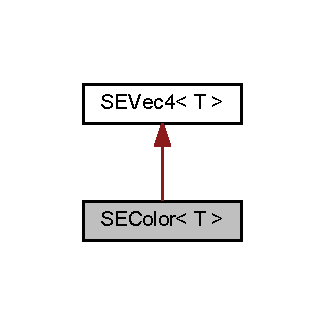
\includegraphics[width=156pt]{class_s_e_color__inherit__graph}
\end{center}
\end{figure}


Collaboration diagram for S\+E\+Color$<$ T $>$\+:
\nopagebreak
\begin{figure}[H]
\begin{center}
\leavevmode
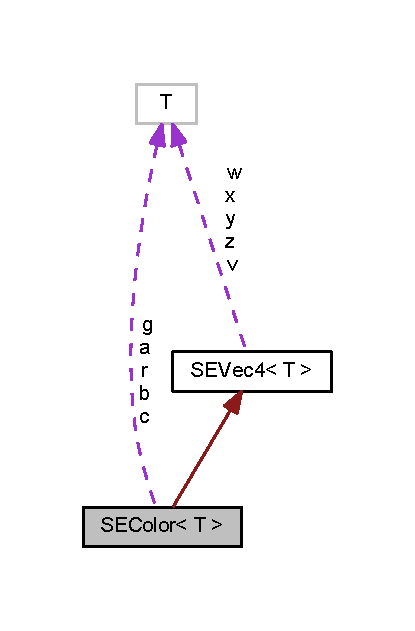
\includegraphics[width=199pt]{class_s_e_color__coll__graph}
\end{center}
\end{figure}
\subsection*{Public Member Functions}
\begin{DoxyCompactItemize}
\item 
{\bf S\+E\+Color} ()
\item 
{\bf S\+E\+Color} (const {\bf S\+E\+Color}$<$ T $>$ \&{\bf c})
\item 
{\bf S\+E\+Color} (T f)
\item 
{\bf S\+E\+Color} (T nr, T ng, T nb)
\item 
{\bf S\+E\+Color} (T nr, T ng, T nb, T na)
\item 
{\bf S\+E\+Color} (const T $\ast$u)
\item 
{\bf S\+E\+Color} (const {\bf S\+E\+Vec3}$<$ T $>$ \&u)
\item 
{\bf S\+E\+Color} (const {\bf S\+E\+Vec4}$<$ T $>$ \&u)
\item 
{\bf S\+E\+Color} (const {\bf S\+E\+Quaternion}$<$ T $>$ \&q)
\item 
{\bf $\sim$\+S\+E\+Color} ()
\item 
{\bf S\+E\+Color}$<$ T $>$ \& {\bf operator=} (const {\bf S\+E\+Color}$<$ T $>$ \&in)
\item 
{\bf S\+E\+Color}$<$ T $>$ \& {\bf operator=} (const {\bf S\+E\+Vec4}$<$ T $>$ \&in)
\item 
{\bf S\+E\+Color}$<$ T $>$ \& {\bf operator=} (const {\bf S\+E\+Vec3}$<$ T $>$ \&in)
\item 
{\bf S\+E\+Color}$<$ T $>$ \& {\bf operator=} (const {\bf S\+E\+Quaternion}$<$ T $>$ \&in)
\item 
{\bf S\+E\+Color}$<$ T $>$ \& {\bf operator+=} (const {\bf S\+E\+Color}$<$ T $>$ \&u)
\item 
{\bf S\+E\+Color}$<$ T $>$ \& {\bf operator+=} (const {\bf S\+E\+Vec4}$<$ T $>$ \&u)
\item 
{\bf S\+E\+Color}$<$ T $>$ \& {\bf operator+=} (const {\bf S\+E\+Vec3}$<$ T $>$ \&u)
\item 
{\bf S\+E\+Color}$<$ T $>$ \& {\bf operator-\/=} (const {\bf S\+E\+Color}$<$ T $>$ \&u)
\item 
{\bf S\+E\+Color}$<$ T $>$ \& {\bf operator-\/=} (const {\bf S\+E\+Vec4}$<$ T $>$ \&u)
\item 
{\bf S\+E\+Color}$<$ T $>$ \& {\bf operator-\/=} (const {\bf S\+E\+Vec3}$<$ T $>$ \&u)
\item 
{\bf S\+E\+Color}$<$ T $>$ \& {\bf operator$\ast$=} (T k)
\item 
{\bf S\+E\+Color}$<$ T $>$ \& {\bf operator/=} (T k)
\item 
T \& {\bf operator[$\,$]} (std\+::size\+\_\+t i)
\item 
const T {\bf operator[$\,$]} (std\+::size\+\_\+t i) const 
\item 
bool {\bf operator==} (const {\bf S\+E\+Color}$<$ T $>$ \&u) const 
\item 
bool {\bf operator!=} (const {\bf S\+E\+Color}$<$ T $>$ \&u) const 
\item 
{\bf S\+E\+Color}$<$ T $>$ \& {\bf set} (T f)
\item 
{\bf S\+E\+Color}$<$ T $>$ \& {\bf set} (T nr, T ng, T nb, T na)
\item 
{\bf S\+E\+Color}$<$ T $>$ \& {\bf set} (T nr, T ng, T nb)
\item 
{\bf S\+E\+Color}$<$ T $>$ \& {\bf set} (const T $\ast$u)
\item 
{\bf S\+E\+Color}$<$ T $>$ \& {\bf set} (const {\bf S\+E\+Vec3}$<$ T $>$ \&u)
\item 
{\bf S\+E\+Color}$<$ T $>$ \& {\bf set} (const {\bf S\+E\+Vec4}$<$ T $>$ \&u)
\item 
{\bf S\+E\+Color}$<$ T $>$ \& {\bf set} (const {\bf S\+E\+Color}$<$ T $>$ \&u)
\item 
{\bf S\+E\+Color}$<$ T $>$ \& {\bf set} (const {\bf S\+E\+Quaternion}$<$ T $>$ \&q)
\item 
{\bf S\+E\+Color}$<$ T $>$ \& {\bf set\+Int\+Values} (int nr, int ng, int nb, int na)
\item 
{\bf S\+E\+Color}$<$ T $>$ \& {\bf set\+Int\+Values} (int nr, int ng, int nb)
\item 
{\bf S\+E\+Color}$<$ T $>$ {\bf mult\+Color} (T f) const 
\item 
{\bf S\+E\+Color}$<$ T $>$ \& {\bf mult\+Color} (T f)
\item 
{\bf S\+E\+Color}$<$ T $>$ {\bf mult\+Alpha} (T f) const 
\item 
{\bf S\+E\+Color}$<$ T $>$ \& {\bf mult\+Alpha} (T f)
\item 
void {\bf clamp} ()
\end{DoxyCompactItemize}
\subsection*{Public Attributes}
\begin{DoxyCompactItemize}
\item 
const T \& {\bf r}
\item 
const T \& {\bf g}
\item 
const T \& {\bf b}
\item 
const T \& {\bf a}
\item 
const T $\ast$ {\bf c}
\end{DoxyCompactItemize}
\subsection*{Friends}
\begin{DoxyCompactItemize}
\item 
{\bf S\+E\+Color}$<$ T $>$ {\bf operator+} ({\bf S\+E\+Color}$<$ T $>$ lhs, {\bf S\+E\+Color}$<$ T $>$ const \&rhs)
\item 
{\bf S\+E\+Color}$<$ T $>$ {\bf operator+} ({\bf S\+E\+Color}$<$ T $>$ lhs, {\bf S\+E\+Vec4}$<$ T $>$ const \&rhs)
\item 
{\bf S\+E\+Color}$<$ T $>$ {\bf operator+} ({\bf S\+E\+Vec4}$<$ T $>$ lhs, {\bf S\+E\+Color}$<$ T $>$ const \&rhs)
\item 
{\bf S\+E\+Color}$<$ T $>$ {\bf operator+} ({\bf S\+E\+Color}$<$ T $>$ lhs, {\bf S\+E\+Vec3}$<$ T $>$ const \&rhs)
\item 
{\bf S\+E\+Color}$<$ T $>$ {\bf operator+} ({\bf S\+E\+Vec3}$<$ T $>$ const \&lhs, {\bf S\+E\+Color}$<$ T $>$ rhs)
\item 
{\bf S\+E\+Color}$<$ T $>$ {\bf operator-\/} ({\bf S\+E\+Color}$<$ T $>$ lhs, {\bf S\+E\+Color}$<$ T $>$ const \&rhs)
\item 
{\bf S\+E\+Color}$<$ T $>$ {\bf operator-\/} ({\bf S\+E\+Color}$<$ T $>$ lhs, {\bf S\+E\+Vec4}$<$ T $>$ const \&rhs)
\item 
{\bf S\+E\+Color}$<$ T $>$ {\bf operator-\/} ({\bf S\+E\+Color}$<$ T $>$ lhs, {\bf S\+E\+Vec3}$<$ T $>$ const \&rhs)
\item 
{\bf S\+E\+Color}$<$ T $>$ {\bf operator$\ast$} ({\bf S\+E\+Color}$<$ T $>$ lhs, T rhs)
\item 
{\bf S\+E\+Color}$<$ T $>$ {\bf operator$\ast$} (T lhs, {\bf S\+E\+Color}$<$ T $>$ rhs)
\item 
{\bf S\+E\+Color}$<$ T $>$ {\bf operator/} ({\bf S\+E\+Color}$<$ T $>$ lhs, T rhs)
\item 
std\+::ostream \& {\bf operator$<$$<$} (std\+::ostream \&os, const {\bf S\+E\+Color}$<$ T $>$ \&u)
\end{DoxyCompactItemize}


\subsection{Detailed Description}
\subsubsection*{template$<$class T$>$class S\+E\+Color$<$ T $>$}



Definition at line 41 of file S\+E\+Math.\+h.



\subsection{Constructor \& Destructor Documentation}
\index{S\+E\+Color@{S\+E\+Color}!S\+E\+Color@{S\+E\+Color}}
\index{S\+E\+Color@{S\+E\+Color}!S\+E\+Color@{S\+E\+Color}}
\subsubsection[{S\+E\+Color}]{\setlength{\rightskip}{0pt plus 5cm}template$<$class T$>$ {\bf S\+E\+Color}$<$ T $>$\+::{\bf S\+E\+Color} (
\begin{DoxyParamCaption}
{}
\end{DoxyParamCaption}
)\hspace{0.3cm}{\ttfamily [inline]}}\label{class_s_e_color_a67574328e6100fea0b7e0a472cff46c0}


Definition at line 406 of file S\+E\+Math.\+h.

\index{S\+E\+Color@{S\+E\+Color}!S\+E\+Color@{S\+E\+Color}}
\index{S\+E\+Color@{S\+E\+Color}!S\+E\+Color@{S\+E\+Color}}
\subsubsection[{S\+E\+Color}]{\setlength{\rightskip}{0pt plus 5cm}template$<$class T$>$ {\bf S\+E\+Color}$<$ T $>$\+::{\bf S\+E\+Color} (
\begin{DoxyParamCaption}
\item[{const {\bf S\+E\+Color}$<$ T $>$ \&}]{c}
\end{DoxyParamCaption}
)\hspace{0.3cm}{\ttfamily [inline]}}\label{class_s_e_color_a6d7dd50fdc33856c38e3a9921c0710bb}


Definition at line 408 of file S\+E\+Math.\+h.

\index{S\+E\+Color@{S\+E\+Color}!S\+E\+Color@{S\+E\+Color}}
\index{S\+E\+Color@{S\+E\+Color}!S\+E\+Color@{S\+E\+Color}}
\subsubsection[{S\+E\+Color}]{\setlength{\rightskip}{0pt plus 5cm}template$<$class T$>$ {\bf S\+E\+Color}$<$ T $>$\+::{\bf S\+E\+Color} (
\begin{DoxyParamCaption}
\item[{T}]{f}
\end{DoxyParamCaption}
)\hspace{0.3cm}{\ttfamily [inline]}, {\ttfamily [explicit]}}\label{class_s_e_color_ac2a0947a9fd96105e5a7bde32dae9fbd}


Definition at line 410 of file S\+E\+Math.\+h.

\index{S\+E\+Color@{S\+E\+Color}!S\+E\+Color@{S\+E\+Color}}
\index{S\+E\+Color@{S\+E\+Color}!S\+E\+Color@{S\+E\+Color}}
\subsubsection[{S\+E\+Color}]{\setlength{\rightskip}{0pt plus 5cm}template$<$class T$>$ {\bf S\+E\+Color}$<$ T $>$\+::{\bf S\+E\+Color} (
\begin{DoxyParamCaption}
\item[{T}]{nr, }
\item[{T}]{ng, }
\item[{T}]{nb}
\end{DoxyParamCaption}
)\hspace{0.3cm}{\ttfamily [inline]}}\label{class_s_e_color_af67c263a2772a9c8503694c5783414d7}


Definition at line 411 of file S\+E\+Math.\+h.

\index{S\+E\+Color@{S\+E\+Color}!S\+E\+Color@{S\+E\+Color}}
\index{S\+E\+Color@{S\+E\+Color}!S\+E\+Color@{S\+E\+Color}}
\subsubsection[{S\+E\+Color}]{\setlength{\rightskip}{0pt plus 5cm}template$<$class T$>$ {\bf S\+E\+Color}$<$ T $>$\+::{\bf S\+E\+Color} (
\begin{DoxyParamCaption}
\item[{T}]{nr, }
\item[{T}]{ng, }
\item[{T}]{nb, }
\item[{T}]{na}
\end{DoxyParamCaption}
)\hspace{0.3cm}{\ttfamily [inline]}}\label{class_s_e_color_a69f23390bd1defe79f6076e7f69a3ef0}


Definition at line 412 of file S\+E\+Math.\+h.

\index{S\+E\+Color@{S\+E\+Color}!S\+E\+Color@{S\+E\+Color}}
\index{S\+E\+Color@{S\+E\+Color}!S\+E\+Color@{S\+E\+Color}}
\subsubsection[{S\+E\+Color}]{\setlength{\rightskip}{0pt plus 5cm}template$<$class T$>$ {\bf S\+E\+Color}$<$ T $>$\+::{\bf S\+E\+Color} (
\begin{DoxyParamCaption}
\item[{const T $\ast$}]{u}
\end{DoxyParamCaption}
)\hspace{0.3cm}{\ttfamily [inline]}, {\ttfamily [explicit]}}\label{class_s_e_color_af3601ae0bea8ad87f542b1d158c0477f}


Definition at line 413 of file S\+E\+Math.\+h.

\index{S\+E\+Color@{S\+E\+Color}!S\+E\+Color@{S\+E\+Color}}
\index{S\+E\+Color@{S\+E\+Color}!S\+E\+Color@{S\+E\+Color}}
\subsubsection[{S\+E\+Color}]{\setlength{\rightskip}{0pt plus 5cm}template$<$class T$>$ {\bf S\+E\+Color}$<$ T $>$\+::{\bf S\+E\+Color} (
\begin{DoxyParamCaption}
\item[{const {\bf S\+E\+Vec3}$<$ T $>$ \&}]{u}
\end{DoxyParamCaption}
)\hspace{0.3cm}{\ttfamily [inline]}}\label{class_s_e_color_a110d246344ed5dd9a4a42001ddc8d7b0}


Definition at line 414 of file S\+E\+Math.\+h.

\index{S\+E\+Color@{S\+E\+Color}!S\+E\+Color@{S\+E\+Color}}
\index{S\+E\+Color@{S\+E\+Color}!S\+E\+Color@{S\+E\+Color}}
\subsubsection[{S\+E\+Color}]{\setlength{\rightskip}{0pt plus 5cm}template$<$class T$>$ {\bf S\+E\+Color}$<$ T $>$\+::{\bf S\+E\+Color} (
\begin{DoxyParamCaption}
\item[{const {\bf S\+E\+Vec4}$<$ T $>$ \&}]{u}
\end{DoxyParamCaption}
)\hspace{0.3cm}{\ttfamily [inline]}}\label{class_s_e_color_acb80d0229d86d6867ced66021c752847}


Definition at line 415 of file S\+E\+Math.\+h.

\index{S\+E\+Color@{S\+E\+Color}!S\+E\+Color@{S\+E\+Color}}
\index{S\+E\+Color@{S\+E\+Color}!S\+E\+Color@{S\+E\+Color}}
\subsubsection[{S\+E\+Color}]{\setlength{\rightskip}{0pt plus 5cm}template$<$class T$>$ {\bf S\+E\+Color}$<$ T $>$\+::{\bf S\+E\+Color} (
\begin{DoxyParamCaption}
\item[{const {\bf S\+E\+Quaternion}$<$ T $>$ \&}]{q}
\end{DoxyParamCaption}
)\hspace{0.3cm}{\ttfamily [inline]}, {\ttfamily [explicit]}}\label{class_s_e_color_a7641268b03286e4c46262e15d99210a0}


Definition at line 416 of file S\+E\+Math.\+h.

\index{S\+E\+Color@{S\+E\+Color}!````~S\+E\+Color@{$\sim$\+S\+E\+Color}}
\index{````~S\+E\+Color@{$\sim$\+S\+E\+Color}!S\+E\+Color@{S\+E\+Color}}
\subsubsection[{$\sim$\+S\+E\+Color}]{\setlength{\rightskip}{0pt plus 5cm}template$<$class T$>$ {\bf S\+E\+Color}$<$ T $>$\+::$\sim${\bf S\+E\+Color} (
\begin{DoxyParamCaption}
{}
\end{DoxyParamCaption}
)\hspace{0.3cm}{\ttfamily [inline]}}\label{class_s_e_color_a9265834f0d9de887647fdcdd06c45728}


Definition at line 419 of file S\+E\+Math.\+h.



\subsection{Member Function Documentation}
\index{S\+E\+Color@{S\+E\+Color}!clamp@{clamp}}
\index{clamp@{clamp}!S\+E\+Color@{S\+E\+Color}}
\subsubsection[{clamp}]{\setlength{\rightskip}{0pt plus 5cm}template$<$class T$>$ void {\bf S\+E\+Color}$<$ T $>$\+::clamp (
\begin{DoxyParamCaption}
{}
\end{DoxyParamCaption}
)\hspace{0.3cm}{\ttfamily [inline]}}\label{class_s_e_color_a38658d53ba81520133bdc80bb0a79676}


Definition at line 472 of file S\+E\+Math.\+h.

\index{S\+E\+Color@{S\+E\+Color}!mult\+Alpha@{mult\+Alpha}}
\index{mult\+Alpha@{mult\+Alpha}!S\+E\+Color@{S\+E\+Color}}
\subsubsection[{mult\+Alpha}]{\setlength{\rightskip}{0pt plus 5cm}template$<$class T$>$ {\bf S\+E\+Color}$<$T$>$ {\bf S\+E\+Color}$<$ T $>$\+::mult\+Alpha (
\begin{DoxyParamCaption}
\item[{T}]{f}
\end{DoxyParamCaption}
) const\hspace{0.3cm}{\ttfamily [inline]}}\label{class_s_e_color_a2130ac8ced0198474891d1e52a1bebdb}


Definition at line 469 of file S\+E\+Math.\+h.

\index{S\+E\+Color@{S\+E\+Color}!mult\+Alpha@{mult\+Alpha}}
\index{mult\+Alpha@{mult\+Alpha}!S\+E\+Color@{S\+E\+Color}}
\subsubsection[{mult\+Alpha}]{\setlength{\rightskip}{0pt plus 5cm}template$<$class T$>$ {\bf S\+E\+Color}$<$T$>$\& {\bf S\+E\+Color}$<$ T $>$\+::mult\+Alpha (
\begin{DoxyParamCaption}
\item[{T}]{f}
\end{DoxyParamCaption}
)\hspace{0.3cm}{\ttfamily [inline]}}\label{class_s_e_color_a7a3ed46a273ea53a8a24dfb84e535e30}


Definition at line 470 of file S\+E\+Math.\+h.

\index{S\+E\+Color@{S\+E\+Color}!mult\+Color@{mult\+Color}}
\index{mult\+Color@{mult\+Color}!S\+E\+Color@{S\+E\+Color}}
\subsubsection[{mult\+Color}]{\setlength{\rightskip}{0pt plus 5cm}template$<$class T$>$ {\bf S\+E\+Color}$<$T$>$ {\bf S\+E\+Color}$<$ T $>$\+::mult\+Color (
\begin{DoxyParamCaption}
\item[{T}]{f}
\end{DoxyParamCaption}
) const\hspace{0.3cm}{\ttfamily [inline]}}\label{class_s_e_color_a4e2818fd3314b30510ef6da1086cb564}


Definition at line 467 of file S\+E\+Math.\+h.

\index{S\+E\+Color@{S\+E\+Color}!mult\+Color@{mult\+Color}}
\index{mult\+Color@{mult\+Color}!S\+E\+Color@{S\+E\+Color}}
\subsubsection[{mult\+Color}]{\setlength{\rightskip}{0pt plus 5cm}template$<$class T$>$ {\bf S\+E\+Color}$<$T$>$\& {\bf S\+E\+Color}$<$ T $>$\+::mult\+Color (
\begin{DoxyParamCaption}
\item[{T}]{f}
\end{DoxyParamCaption}
)\hspace{0.3cm}{\ttfamily [inline]}}\label{class_s_e_color_ae9b8556b4c9fff431111ff825e5d4e7c}


Definition at line 468 of file S\+E\+Math.\+h.

\index{S\+E\+Color@{S\+E\+Color}!operator"!=@{operator"!=}}
\index{operator"!=@{operator"!=}!S\+E\+Color@{S\+E\+Color}}
\subsubsection[{operator"!=}]{\setlength{\rightskip}{0pt plus 5cm}template$<$class T$>$ bool {\bf S\+E\+Color}$<$ T $>$\+::operator!= (
\begin{DoxyParamCaption}
\item[{const {\bf S\+E\+Color}$<$ T $>$ \&}]{u}
\end{DoxyParamCaption}
) const\hspace{0.3cm}{\ttfamily [inline]}}\label{class_s_e_color_ada8719ec26661e78b3cfdfb660e58ac2}


Definition at line 451 of file S\+E\+Math.\+h.

\index{S\+E\+Color@{S\+E\+Color}!operator$\ast$=@{operator$\ast$=}}
\index{operator$\ast$=@{operator$\ast$=}!S\+E\+Color@{S\+E\+Color}}
\subsubsection[{operator$\ast$=}]{\setlength{\rightskip}{0pt plus 5cm}template$<$class T$>$ {\bf S\+E\+Color}$<$T$>$\& {\bf S\+E\+Color}$<$ T $>$\+::operator$\ast$= (
\begin{DoxyParamCaption}
\item[{T}]{k}
\end{DoxyParamCaption}
)\hspace{0.3cm}{\ttfamily [inline]}}\label{class_s_e_color_a0bc013ef7810b9740a064e8834ad0083}


Definition at line 432 of file S\+E\+Math.\+h.

\index{S\+E\+Color@{S\+E\+Color}!operator+=@{operator+=}}
\index{operator+=@{operator+=}!S\+E\+Color@{S\+E\+Color}}
\subsubsection[{operator+=}]{\setlength{\rightskip}{0pt plus 5cm}template$<$class T$>$ {\bf S\+E\+Color}$<$T$>$\& {\bf S\+E\+Color}$<$ T $>$\+::operator+= (
\begin{DoxyParamCaption}
\item[{const {\bf S\+E\+Color}$<$ T $>$ \&}]{u}
\end{DoxyParamCaption}
)\hspace{0.3cm}{\ttfamily [inline]}}\label{class_s_e_color_a33c8fcd606dfd560bdd69f5882649b54}


Definition at line 426 of file S\+E\+Math.\+h.

\index{S\+E\+Color@{S\+E\+Color}!operator+=@{operator+=}}
\index{operator+=@{operator+=}!S\+E\+Color@{S\+E\+Color}}
\subsubsection[{operator+=}]{\setlength{\rightskip}{0pt plus 5cm}template$<$class T$>$ {\bf S\+E\+Color}$<$T$>$\& {\bf S\+E\+Color}$<$ T $>$\+::operator+= (
\begin{DoxyParamCaption}
\item[{const {\bf S\+E\+Vec4}$<$ T $>$ \&}]{u}
\end{DoxyParamCaption}
)\hspace{0.3cm}{\ttfamily [inline]}}\label{class_s_e_color_aabb844d86ee4c2d8d70db96a2732f0fc}


Definition at line 427 of file S\+E\+Math.\+h.

\index{S\+E\+Color@{S\+E\+Color}!operator+=@{operator+=}}
\index{operator+=@{operator+=}!S\+E\+Color@{S\+E\+Color}}
\subsubsection[{operator+=}]{\setlength{\rightskip}{0pt plus 5cm}template$<$class T$>$ {\bf S\+E\+Color}$<$T$>$\& {\bf S\+E\+Color}$<$ T $>$\+::operator+= (
\begin{DoxyParamCaption}
\item[{const {\bf S\+E\+Vec3}$<$ T $>$ \&}]{u}
\end{DoxyParamCaption}
)\hspace{0.3cm}{\ttfamily [inline]}}\label{class_s_e_color_ae3579e6f23e0ce0cd8a63c0871740960}


Definition at line 428 of file S\+E\+Math.\+h.

\index{S\+E\+Color@{S\+E\+Color}!operator-\/=@{operator-\/=}}
\index{operator-\/=@{operator-\/=}!S\+E\+Color@{S\+E\+Color}}
\subsubsection[{operator-\/=}]{\setlength{\rightskip}{0pt plus 5cm}template$<$class T$>$ {\bf S\+E\+Color}$<$T$>$\& {\bf S\+E\+Color}$<$ T $>$\+::operator-\/= (
\begin{DoxyParamCaption}
\item[{const {\bf S\+E\+Color}$<$ T $>$ \&}]{u}
\end{DoxyParamCaption}
)\hspace{0.3cm}{\ttfamily [inline]}}\label{class_s_e_color_a3650f86c50a044878988e52d23294e54}


Definition at line 429 of file S\+E\+Math.\+h.

\index{S\+E\+Color@{S\+E\+Color}!operator-\/=@{operator-\/=}}
\index{operator-\/=@{operator-\/=}!S\+E\+Color@{S\+E\+Color}}
\subsubsection[{operator-\/=}]{\setlength{\rightskip}{0pt plus 5cm}template$<$class T$>$ {\bf S\+E\+Color}$<$T$>$\& {\bf S\+E\+Color}$<$ T $>$\+::operator-\/= (
\begin{DoxyParamCaption}
\item[{const {\bf S\+E\+Vec4}$<$ T $>$ \&}]{u}
\end{DoxyParamCaption}
)\hspace{0.3cm}{\ttfamily [inline]}}\label{class_s_e_color_a0978f4225129a8e8347d6ff35b03f222}


Definition at line 430 of file S\+E\+Math.\+h.

\index{S\+E\+Color@{S\+E\+Color}!operator-\/=@{operator-\/=}}
\index{operator-\/=@{operator-\/=}!S\+E\+Color@{S\+E\+Color}}
\subsubsection[{operator-\/=}]{\setlength{\rightskip}{0pt plus 5cm}template$<$class T$>$ {\bf S\+E\+Color}$<$T$>$\& {\bf S\+E\+Color}$<$ T $>$\+::operator-\/= (
\begin{DoxyParamCaption}
\item[{const {\bf S\+E\+Vec3}$<$ T $>$ \&}]{u}
\end{DoxyParamCaption}
)\hspace{0.3cm}{\ttfamily [inline]}}\label{class_s_e_color_a68eee610316c5bfcf0fc86a155f381f2}


Definition at line 431 of file S\+E\+Math.\+h.

\index{S\+E\+Color@{S\+E\+Color}!operator/=@{operator/=}}
\index{operator/=@{operator/=}!S\+E\+Color@{S\+E\+Color}}
\subsubsection[{operator/=}]{\setlength{\rightskip}{0pt plus 5cm}template$<$class T$>$ {\bf S\+E\+Color}$<$T$>$\& {\bf S\+E\+Color}$<$ T $>$\+::operator/= (
\begin{DoxyParamCaption}
\item[{T}]{k}
\end{DoxyParamCaption}
)\hspace{0.3cm}{\ttfamily [inline]}}\label{class_s_e_color_a20735100c75c136944f3bec657c70c79}


Definition at line 433 of file S\+E\+Math.\+h.

\index{S\+E\+Color@{S\+E\+Color}!operator=@{operator=}}
\index{operator=@{operator=}!S\+E\+Color@{S\+E\+Color}}
\subsubsection[{operator=}]{\setlength{\rightskip}{0pt plus 5cm}template$<$class T$>$ {\bf S\+E\+Color}$<$T$>$\& {\bf S\+E\+Color}$<$ T $>$\+::operator= (
\begin{DoxyParamCaption}
\item[{const {\bf S\+E\+Color}$<$ T $>$ \&}]{in}
\end{DoxyParamCaption}
)\hspace{0.3cm}{\ttfamily [inline]}}\label{class_s_e_color_ae4ead9bfaf749c622e08690e25c6214b}


Definition at line 421 of file S\+E\+Math.\+h.

\index{S\+E\+Color@{S\+E\+Color}!operator=@{operator=}}
\index{operator=@{operator=}!S\+E\+Color@{S\+E\+Color}}
\subsubsection[{operator=}]{\setlength{\rightskip}{0pt plus 5cm}template$<$class T$>$ {\bf S\+E\+Color}$<$T$>$\& {\bf S\+E\+Color}$<$ T $>$\+::operator= (
\begin{DoxyParamCaption}
\item[{const {\bf S\+E\+Vec4}$<$ T $>$ \&}]{in}
\end{DoxyParamCaption}
)\hspace{0.3cm}{\ttfamily [inline]}}\label{class_s_e_color_aa9a2bd323c2cc87973d37f26eb977b48}


Definition at line 422 of file S\+E\+Math.\+h.

\index{S\+E\+Color@{S\+E\+Color}!operator=@{operator=}}
\index{operator=@{operator=}!S\+E\+Color@{S\+E\+Color}}
\subsubsection[{operator=}]{\setlength{\rightskip}{0pt plus 5cm}template$<$class T$>$ {\bf S\+E\+Color}$<$T$>$\& {\bf S\+E\+Color}$<$ T $>$\+::operator= (
\begin{DoxyParamCaption}
\item[{const {\bf S\+E\+Vec3}$<$ T $>$ \&}]{in}
\end{DoxyParamCaption}
)\hspace{0.3cm}{\ttfamily [inline]}}\label{class_s_e_color_ad916fdf3f4b69ab7a4063c35a9fcea51}


Definition at line 423 of file S\+E\+Math.\+h.

\index{S\+E\+Color@{S\+E\+Color}!operator=@{operator=}}
\index{operator=@{operator=}!S\+E\+Color@{S\+E\+Color}}
\subsubsection[{operator=}]{\setlength{\rightskip}{0pt plus 5cm}template$<$class T$>$ {\bf S\+E\+Color}$<$T$>$\& {\bf S\+E\+Color}$<$ T $>$\+::operator= (
\begin{DoxyParamCaption}
\item[{const {\bf S\+E\+Quaternion}$<$ T $>$ \&}]{in}
\end{DoxyParamCaption}
)\hspace{0.3cm}{\ttfamily [inline]}}\label{class_s_e_color_aae65a9fe725a0229584ca382902eecfd}


Definition at line 424 of file S\+E\+Math.\+h.

\index{S\+E\+Color@{S\+E\+Color}!operator==@{operator==}}
\index{operator==@{operator==}!S\+E\+Color@{S\+E\+Color}}
\subsubsection[{operator==}]{\setlength{\rightskip}{0pt plus 5cm}template$<$class T$>$ bool {\bf S\+E\+Color}$<$ T $>$\+::operator== (
\begin{DoxyParamCaption}
\item[{const {\bf S\+E\+Color}$<$ T $>$ \&}]{u}
\end{DoxyParamCaption}
) const\hspace{0.3cm}{\ttfamily [inline]}}\label{class_s_e_color_a21b05f45067f56552ac8dfb5388e26c9}


Definition at line 450 of file S\+E\+Math.\+h.

\index{S\+E\+Color@{S\+E\+Color}!operator[$\,$]@{operator[]}}
\index{operator[$\,$]@{operator[]}!S\+E\+Color@{S\+E\+Color}}
\subsubsection[{operator[]}]{\setlength{\rightskip}{0pt plus 5cm}template$<$class T$>$ T\& {\bf S\+E\+Color}$<$ T $>$\+::operator[$\,$] (
\begin{DoxyParamCaption}
\item[{std\+::size\+\_\+t}]{i}
\end{DoxyParamCaption}
)\hspace{0.3cm}{\ttfamily [inline]}}\label{class_s_e_color_a0267fbae2e64e174d65a867e2f11902b}


Definition at line 447 of file S\+E\+Math.\+h.

\index{S\+E\+Color@{S\+E\+Color}!operator[$\,$]@{operator[]}}
\index{operator[$\,$]@{operator[]}!S\+E\+Color@{S\+E\+Color}}
\subsubsection[{operator[]}]{\setlength{\rightskip}{0pt plus 5cm}template$<$class T$>$ const T {\bf S\+E\+Color}$<$ T $>$\+::operator[$\,$] (
\begin{DoxyParamCaption}
\item[{std\+::size\+\_\+t}]{i}
\end{DoxyParamCaption}
) const\hspace{0.3cm}{\ttfamily [inline]}}\label{class_s_e_color_a5f92036c10db0a73e1daee266df0483a}


Definition at line 448 of file S\+E\+Math.\+h.

\index{S\+E\+Color@{S\+E\+Color}!set@{set}}
\index{set@{set}!S\+E\+Color@{S\+E\+Color}}
\subsubsection[{set}]{\setlength{\rightskip}{0pt plus 5cm}template$<$class T$>$ {\bf S\+E\+Color}$<$T$>$\& {\bf S\+E\+Color}$<$ T $>$\+::set (
\begin{DoxyParamCaption}
\item[{T}]{f}
\end{DoxyParamCaption}
)\hspace{0.3cm}{\ttfamily [inline]}}\label{class_s_e_color_a281bd9c1a2ef27112997010060524262}


Definition at line 455 of file S\+E\+Math.\+h.

\index{S\+E\+Color@{S\+E\+Color}!set@{set}}
\index{set@{set}!S\+E\+Color@{S\+E\+Color}}
\subsubsection[{set}]{\setlength{\rightskip}{0pt plus 5cm}template$<$class T$>$ {\bf S\+E\+Color}$<$T$>$\& {\bf S\+E\+Color}$<$ T $>$\+::set (
\begin{DoxyParamCaption}
\item[{T}]{nr, }
\item[{T}]{ng, }
\item[{T}]{nb, }
\item[{T}]{na}
\end{DoxyParamCaption}
)\hspace{0.3cm}{\ttfamily [inline]}}\label{class_s_e_color_a771488421c6305fef6dd3f693ad2d06b}


Definition at line 456 of file S\+E\+Math.\+h.

\index{S\+E\+Color@{S\+E\+Color}!set@{set}}
\index{set@{set}!S\+E\+Color@{S\+E\+Color}}
\subsubsection[{set}]{\setlength{\rightskip}{0pt plus 5cm}template$<$class T$>$ {\bf S\+E\+Color}$<$T$>$\& {\bf S\+E\+Color}$<$ T $>$\+::set (
\begin{DoxyParamCaption}
\item[{T}]{nr, }
\item[{T}]{ng, }
\item[{T}]{nb}
\end{DoxyParamCaption}
)\hspace{0.3cm}{\ttfamily [inline]}}\label{class_s_e_color_ab58e4944983145da0d6e5e1b4d808fc4}


Definition at line 457 of file S\+E\+Math.\+h.

\index{S\+E\+Color@{S\+E\+Color}!set@{set}}
\index{set@{set}!S\+E\+Color@{S\+E\+Color}}
\subsubsection[{set}]{\setlength{\rightskip}{0pt plus 5cm}template$<$class T$>$ {\bf S\+E\+Color}$<$T$>$\& {\bf S\+E\+Color}$<$ T $>$\+::set (
\begin{DoxyParamCaption}
\item[{const T $\ast$}]{u}
\end{DoxyParamCaption}
)\hspace{0.3cm}{\ttfamily [inline]}}\label{class_s_e_color_a86326dadb478cee603279319aee0ed2e}


Definition at line 458 of file S\+E\+Math.\+h.

\index{S\+E\+Color@{S\+E\+Color}!set@{set}}
\index{set@{set}!S\+E\+Color@{S\+E\+Color}}
\subsubsection[{set}]{\setlength{\rightskip}{0pt plus 5cm}template$<$class T$>$ {\bf S\+E\+Color}$<$T$>$\& {\bf S\+E\+Color}$<$ T $>$\+::set (
\begin{DoxyParamCaption}
\item[{const {\bf S\+E\+Vec3}$<$ T $>$ \&}]{u}
\end{DoxyParamCaption}
)\hspace{0.3cm}{\ttfamily [inline]}}\label{class_s_e_color_a5ecb57f66a3d328f67c04a1a0c6338fa}


Definition at line 459 of file S\+E\+Math.\+h.

\index{S\+E\+Color@{S\+E\+Color}!set@{set}}
\index{set@{set}!S\+E\+Color@{S\+E\+Color}}
\subsubsection[{set}]{\setlength{\rightskip}{0pt plus 5cm}template$<$class T$>$ {\bf S\+E\+Color}$<$T$>$\& {\bf S\+E\+Color}$<$ T $>$\+::set (
\begin{DoxyParamCaption}
\item[{const {\bf S\+E\+Vec4}$<$ T $>$ \&}]{u}
\end{DoxyParamCaption}
)\hspace{0.3cm}{\ttfamily [inline]}}\label{class_s_e_color_a4e725940b92d114941ad68f4ef75447d}


Definition at line 460 of file S\+E\+Math.\+h.

\index{S\+E\+Color@{S\+E\+Color}!set@{set}}
\index{set@{set}!S\+E\+Color@{S\+E\+Color}}
\subsubsection[{set}]{\setlength{\rightskip}{0pt plus 5cm}template$<$class T$>$ {\bf S\+E\+Color}$<$T$>$\& {\bf S\+E\+Color}$<$ T $>$\+::set (
\begin{DoxyParamCaption}
\item[{const {\bf S\+E\+Color}$<$ T $>$ \&}]{u}
\end{DoxyParamCaption}
)\hspace{0.3cm}{\ttfamily [inline]}}\label{class_s_e_color_a89de39cfc7930c92ee059edcbb612dcb}


Definition at line 461 of file S\+E\+Math.\+h.

\index{S\+E\+Color@{S\+E\+Color}!set@{set}}
\index{set@{set}!S\+E\+Color@{S\+E\+Color}}
\subsubsection[{set}]{\setlength{\rightskip}{0pt plus 5cm}template$<$class T$>$ {\bf S\+E\+Color}$<$T$>$\& {\bf S\+E\+Color}$<$ T $>$\+::set (
\begin{DoxyParamCaption}
\item[{const {\bf S\+E\+Quaternion}$<$ T $>$ \&}]{q}
\end{DoxyParamCaption}
)\hspace{0.3cm}{\ttfamily [inline]}}\label{class_s_e_color_a704b62425136362bc7f5eaf070b96c80}


Definition at line 462 of file S\+E\+Math.\+h.

\index{S\+E\+Color@{S\+E\+Color}!set\+Int\+Values@{set\+Int\+Values}}
\index{set\+Int\+Values@{set\+Int\+Values}!S\+E\+Color@{S\+E\+Color}}
\subsubsection[{set\+Int\+Values}]{\setlength{\rightskip}{0pt plus 5cm}template$<$class T$>$ {\bf S\+E\+Color}$<$T$>$\& {\bf S\+E\+Color}$<$ T $>$\+::set\+Int\+Values (
\begin{DoxyParamCaption}
\item[{int}]{nr, }
\item[{int}]{ng, }
\item[{int}]{nb, }
\item[{int}]{na}
\end{DoxyParamCaption}
)\hspace{0.3cm}{\ttfamily [inline]}}\label{class_s_e_color_a05e7ed6e7311925961fdb15788959c3d}


Definition at line 464 of file S\+E\+Math.\+h.

\index{S\+E\+Color@{S\+E\+Color}!set\+Int\+Values@{set\+Int\+Values}}
\index{set\+Int\+Values@{set\+Int\+Values}!S\+E\+Color@{S\+E\+Color}}
\subsubsection[{set\+Int\+Values}]{\setlength{\rightskip}{0pt plus 5cm}template$<$class T$>$ {\bf S\+E\+Color}$<$T$>$\& {\bf S\+E\+Color}$<$ T $>$\+::set\+Int\+Values (
\begin{DoxyParamCaption}
\item[{int}]{nr, }
\item[{int}]{ng, }
\item[{int}]{nb}
\end{DoxyParamCaption}
)\hspace{0.3cm}{\ttfamily [inline]}}\label{class_s_e_color_a46b296d0be98e7c9bd0337935dff2da6}


Definition at line 465 of file S\+E\+Math.\+h.



\subsection{Friends And Related Function Documentation}
\index{S\+E\+Color@{S\+E\+Color}!operator$\ast$@{operator$\ast$}}
\index{operator$\ast$@{operator$\ast$}!S\+E\+Color@{S\+E\+Color}}
\subsubsection[{operator$\ast$}]{\setlength{\rightskip}{0pt plus 5cm}template$<$class T$>$ {\bf S\+E\+Color}$<$T$>$ operator$\ast$ (
\begin{DoxyParamCaption}
\item[{{\bf S\+E\+Color}$<$ T $>$}]{lhs, }
\item[{T}]{rhs}
\end{DoxyParamCaption}
)\hspace{0.3cm}{\ttfamily [friend]}}\label{class_s_e_color_a7f58e3a825f2ef884a5af79379080620}


Definition at line 443 of file S\+E\+Math.\+h.

\index{S\+E\+Color@{S\+E\+Color}!operator$\ast$@{operator$\ast$}}
\index{operator$\ast$@{operator$\ast$}!S\+E\+Color@{S\+E\+Color}}
\subsubsection[{operator$\ast$}]{\setlength{\rightskip}{0pt plus 5cm}template$<$class T$>$ {\bf S\+E\+Color}$<$T$>$ operator$\ast$ (
\begin{DoxyParamCaption}
\item[{T}]{lhs, }
\item[{{\bf S\+E\+Color}$<$ T $>$}]{rhs}
\end{DoxyParamCaption}
)\hspace{0.3cm}{\ttfamily [friend]}}\label{class_s_e_color_a96bd0d21e30e69ff97d3fc0b6184126d}


Definition at line 444 of file S\+E\+Math.\+h.

\index{S\+E\+Color@{S\+E\+Color}!operator+@{operator+}}
\index{operator+@{operator+}!S\+E\+Color@{S\+E\+Color}}
\subsubsection[{operator+}]{\setlength{\rightskip}{0pt plus 5cm}template$<$class T$>$ {\bf S\+E\+Color}$<$T$>$ operator+ (
\begin{DoxyParamCaption}
\item[{{\bf S\+E\+Color}$<$ T $>$}]{lhs, }
\item[{{\bf S\+E\+Color}$<$ T $>$ const \&}]{rhs}
\end{DoxyParamCaption}
)\hspace{0.3cm}{\ttfamily [friend]}}\label{class_s_e_color_a6f453b0206a4dbf0c7c1f351f99a91c2}


Definition at line 435 of file S\+E\+Math.\+h.

\index{S\+E\+Color@{S\+E\+Color}!operator+@{operator+}}
\index{operator+@{operator+}!S\+E\+Color@{S\+E\+Color}}
\subsubsection[{operator+}]{\setlength{\rightskip}{0pt plus 5cm}template$<$class T$>$ {\bf S\+E\+Color}$<$T$>$ operator+ (
\begin{DoxyParamCaption}
\item[{{\bf S\+E\+Color}$<$ T $>$}]{lhs, }
\item[{{\bf S\+E\+Vec4}$<$ T $>$ const \&}]{rhs}
\end{DoxyParamCaption}
)\hspace{0.3cm}{\ttfamily [friend]}}\label{class_s_e_color_ab74a3db5121898bd2ae7f2dbd3c9539a}


Definition at line 436 of file S\+E\+Math.\+h.

\index{S\+E\+Color@{S\+E\+Color}!operator+@{operator+}}
\index{operator+@{operator+}!S\+E\+Color@{S\+E\+Color}}
\subsubsection[{operator+}]{\setlength{\rightskip}{0pt plus 5cm}template$<$class T$>$ {\bf S\+E\+Color}$<$T$>$ operator+ (
\begin{DoxyParamCaption}
\item[{{\bf S\+E\+Vec4}$<$ T $>$}]{lhs, }
\item[{{\bf S\+E\+Color}$<$ T $>$ const \&}]{rhs}
\end{DoxyParamCaption}
)\hspace{0.3cm}{\ttfamily [friend]}}\label{class_s_e_color_a9dc0f4d5b6f203710b71b80a0778376f}


Definition at line 437 of file S\+E\+Math.\+h.

\index{S\+E\+Color@{S\+E\+Color}!operator+@{operator+}}
\index{operator+@{operator+}!S\+E\+Color@{S\+E\+Color}}
\subsubsection[{operator+}]{\setlength{\rightskip}{0pt plus 5cm}template$<$class T$>$ {\bf S\+E\+Color}$<$T$>$ operator+ (
\begin{DoxyParamCaption}
\item[{{\bf S\+E\+Color}$<$ T $>$}]{lhs, }
\item[{{\bf S\+E\+Vec3}$<$ T $>$ const \&}]{rhs}
\end{DoxyParamCaption}
)\hspace{0.3cm}{\ttfamily [friend]}}\label{class_s_e_color_aa28d616d61fc47fc09384eda4482ee57}


Definition at line 438 of file S\+E\+Math.\+h.

\index{S\+E\+Color@{S\+E\+Color}!operator+@{operator+}}
\index{operator+@{operator+}!S\+E\+Color@{S\+E\+Color}}
\subsubsection[{operator+}]{\setlength{\rightskip}{0pt plus 5cm}template$<$class T$>$ {\bf S\+E\+Color}$<$T$>$ operator+ (
\begin{DoxyParamCaption}
\item[{{\bf S\+E\+Vec3}$<$ T $>$ const \&}]{lhs, }
\item[{{\bf S\+E\+Color}$<$ T $>$}]{rhs}
\end{DoxyParamCaption}
)\hspace{0.3cm}{\ttfamily [friend]}}\label{class_s_e_color_a3d9cd8697ceb54cff39987447ddaa3c9}


Definition at line 439 of file S\+E\+Math.\+h.

\index{S\+E\+Color@{S\+E\+Color}!operator-\/@{operator-\/}}
\index{operator-\/@{operator-\/}!S\+E\+Color@{S\+E\+Color}}
\subsubsection[{operator-\/}]{\setlength{\rightskip}{0pt plus 5cm}template$<$class T$>$ {\bf S\+E\+Color}$<$T$>$ operator-\/ (
\begin{DoxyParamCaption}
\item[{{\bf S\+E\+Color}$<$ T $>$}]{lhs, }
\item[{{\bf S\+E\+Color}$<$ T $>$ const \&}]{rhs}
\end{DoxyParamCaption}
)\hspace{0.3cm}{\ttfamily [friend]}}\label{class_s_e_color_ad4521838bc354cbea4517640debaac06}


Definition at line 440 of file S\+E\+Math.\+h.

\index{S\+E\+Color@{S\+E\+Color}!operator-\/@{operator-\/}}
\index{operator-\/@{operator-\/}!S\+E\+Color@{S\+E\+Color}}
\subsubsection[{operator-\/}]{\setlength{\rightskip}{0pt plus 5cm}template$<$class T$>$ {\bf S\+E\+Color}$<$T$>$ operator-\/ (
\begin{DoxyParamCaption}
\item[{{\bf S\+E\+Color}$<$ T $>$}]{lhs, }
\item[{{\bf S\+E\+Vec4}$<$ T $>$ const \&}]{rhs}
\end{DoxyParamCaption}
)\hspace{0.3cm}{\ttfamily [friend]}}\label{class_s_e_color_ae4d194d9a8907dabfc128c96d2bf2387}


Definition at line 441 of file S\+E\+Math.\+h.

\index{S\+E\+Color@{S\+E\+Color}!operator-\/@{operator-\/}}
\index{operator-\/@{operator-\/}!S\+E\+Color@{S\+E\+Color}}
\subsubsection[{operator-\/}]{\setlength{\rightskip}{0pt plus 5cm}template$<$class T$>$ {\bf S\+E\+Color}$<$T$>$ operator-\/ (
\begin{DoxyParamCaption}
\item[{{\bf S\+E\+Color}$<$ T $>$}]{lhs, }
\item[{{\bf S\+E\+Vec3}$<$ T $>$ const \&}]{rhs}
\end{DoxyParamCaption}
)\hspace{0.3cm}{\ttfamily [friend]}}\label{class_s_e_color_a1a4c3c11c5a0b63ffd3a0a8ca05f7a9d}


Definition at line 442 of file S\+E\+Math.\+h.

\index{S\+E\+Color@{S\+E\+Color}!operator/@{operator/}}
\index{operator/@{operator/}!S\+E\+Color@{S\+E\+Color}}
\subsubsection[{operator/}]{\setlength{\rightskip}{0pt plus 5cm}template$<$class T$>$ {\bf S\+E\+Color}$<$T$>$ operator/ (
\begin{DoxyParamCaption}
\item[{{\bf S\+E\+Color}$<$ T $>$}]{lhs, }
\item[{T}]{rhs}
\end{DoxyParamCaption}
)\hspace{0.3cm}{\ttfamily [friend]}}\label{class_s_e_color_af9f75ac5d275b838079635b9cf11e51d}


Definition at line 445 of file S\+E\+Math.\+h.

\index{S\+E\+Color@{S\+E\+Color}!operator$<$$<$@{operator$<$$<$}}
\index{operator$<$$<$@{operator$<$$<$}!S\+E\+Color@{S\+E\+Color}}
\subsubsection[{operator$<$$<$}]{\setlength{\rightskip}{0pt plus 5cm}template$<$class T$>$ std\+::ostream\& operator$<$$<$ (
\begin{DoxyParamCaption}
\item[{std\+::ostream \&}]{os, }
\item[{const {\bf S\+E\+Color}$<$ T $>$ \&}]{u}
\end{DoxyParamCaption}
)\hspace{0.3cm}{\ttfamily [friend]}}\label{class_s_e_color_a58568cb9ec78bd0634662b00f1993d7a}


Definition at line 453 of file S\+E\+Math.\+h.



\subsection{Member Data Documentation}
\index{S\+E\+Color@{S\+E\+Color}!a@{a}}
\index{a@{a}!S\+E\+Color@{S\+E\+Color}}
\subsubsection[{a}]{\setlength{\rightskip}{0pt plus 5cm}template$<$class T$>$ const T \& {\bf S\+E\+Color}$<$ T $>$\+::a}\label{class_s_e_color_a56b9d8e56a22775098a8bec54c21f93e}


Definition at line 402 of file S\+E\+Math.\+h.

\index{S\+E\+Color@{S\+E\+Color}!b@{b}}
\index{b@{b}!S\+E\+Color@{S\+E\+Color}}
\subsubsection[{b}]{\setlength{\rightskip}{0pt plus 5cm}template$<$class T$>$ const T \& {\bf S\+E\+Color}$<$ T $>$\+::b}\label{class_s_e_color_af087334bc49c13128771a402eda77b7a}


Definition at line 402 of file S\+E\+Math.\+h.

\index{S\+E\+Color@{S\+E\+Color}!c@{c}}
\index{c@{c}!S\+E\+Color@{S\+E\+Color}}
\subsubsection[{c}]{\setlength{\rightskip}{0pt plus 5cm}template$<$class T$>$ const T$\ast$ {\bf S\+E\+Color}$<$ T $>$\+::c}\label{class_s_e_color_a1adf2eee31e497a0b63424a000d7588c}


Definition at line 403 of file S\+E\+Math.\+h.

\index{S\+E\+Color@{S\+E\+Color}!g@{g}}
\index{g@{g}!S\+E\+Color@{S\+E\+Color}}
\subsubsection[{g}]{\setlength{\rightskip}{0pt plus 5cm}template$<$class T$>$ const T \& {\bf S\+E\+Color}$<$ T $>$\+::g}\label{class_s_e_color_a3dce3c2fb858a72ae9bca692e90fc372}


Definition at line 402 of file S\+E\+Math.\+h.

\index{S\+E\+Color@{S\+E\+Color}!r@{r}}
\index{r@{r}!S\+E\+Color@{S\+E\+Color}}
\subsubsection[{r}]{\setlength{\rightskip}{0pt plus 5cm}template$<$class T$>$ const T\& {\bf S\+E\+Color}$<$ T $>$\+::r}\label{class_s_e_color_a1dd483a2cca555347a0c01d5da7470d9}


Definition at line 402 of file S\+E\+Math.\+h.



The documentation for this class was generated from the following file\+:\begin{DoxyCompactItemize}
\item 
{\bf S\+E\+Math.\+h}\end{DoxyCompactItemize}

\section{S\+E\+Component Class Reference}
\label{class_s_e_component}\index{S\+E\+Component@{S\+E\+Component}}


{\ttfamily \#include $<$S\+E\+Component.\+h$>$}



Inheritance diagram for S\+E\+Component\+:
\nopagebreak
\begin{figure}[H]
\begin{center}
\leavevmode
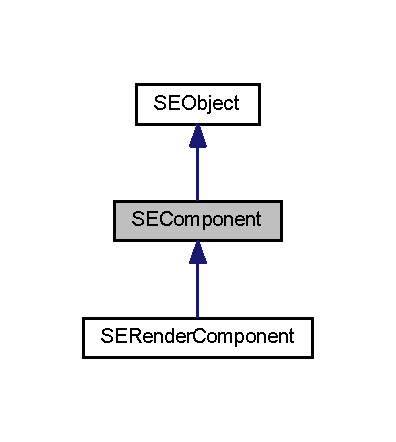
\includegraphics[width=190pt]{class_s_e_component__inherit__graph}
\end{center}
\end{figure}


Collaboration diagram for S\+E\+Component\+:
\nopagebreak
\begin{figure}[H]
\begin{center}
\leavevmode
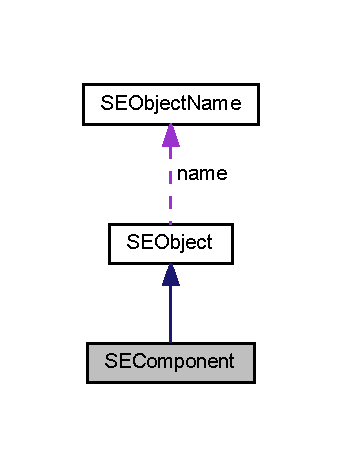
\includegraphics[width=164pt]{class_s_e_component__coll__graph}
\end{center}
\end{figure}
\subsection*{Public Types}
\begin{DoxyCompactItemize}
\item 
enum {\bf t\+Component} \{ \\*
{\bf R\+E\+N\+D\+E\+R\+\_\+\+C\+O\+M\+P\+O\+N\+E\+N\+T}, 
{\bf T\+I\+M\+E\+R\+\_\+\+C\+O\+M\+P\+O\+N\+E\+N\+T}, 
{\bf P\+H\+Y\+S\+I\+C\+S\+\_\+\+C\+O\+M\+P\+O\+N\+E\+N\+T}, 
{\bf A\+N\+I\+M\+A\+T\+I\+O\+N\+\_\+\+C\+O\+M\+P\+O\+N\+E\+N\+T}, 
\\*
{\bf U\+I\+\_\+\+C\+O\+M\+P\+O\+N\+E\+N\+T}, 
{\bf A\+U\+D\+I\+O\+\_\+\+C\+O\+M\+P\+O\+N\+E\+N\+T}, 
{\bf C\+O\+N\+T\+R\+O\+L\+\_\+\+C\+O\+M\+P\+O\+N\+E\+N\+T}, 
{\bf S\+T\+A\+T\+E\+M\+A\+C\+H\+I\+N\+E\+\_\+\+C\+O\+M\+P\+O\+N\+E\+N\+T}, 
\\*
{\bf N\+U\+M\+\_\+\+C\+O\+M\+P\+O\+N\+E\+N\+T\+S}
 \}
\end{DoxyCompactItemize}
\subsection*{Public Member Functions}
\begin{DoxyCompactItemize}
\item 
virtual void {\bf update} (double dt)=0
\item 
virtual {\bf t\+Component} {\bf type} ()=0
\item 
{\bf $\sim$\+S\+E\+Component} ()
\end{DoxyCompactItemize}
\subsection*{Protected Member Functions}
\begin{DoxyCompactItemize}
\item 
{\bf S\+E\+Component} ({\bf t\+Component} t)
\end{DoxyCompactItemize}
\subsection*{Protected Attributes}
\begin{DoxyCompactItemize}
\item 
{\bf t\+Component} {\bf t\+\_\+}
\end{DoxyCompactItemize}
\subsection*{Additional Inherited Members}


\subsection{Detailed Description}


Definition at line 6 of file S\+E\+Component.\+h.



\subsection{Member Enumeration Documentation}
\index{S\+E\+Component@{S\+E\+Component}!t\+Component@{t\+Component}}
\index{t\+Component@{t\+Component}!S\+E\+Component@{S\+E\+Component}}
\subsubsection[{t\+Component}]{\setlength{\rightskip}{0pt plus 5cm}enum {\bf S\+E\+Component\+::t\+Component}}\label{class_s_e_component_a3df61ea419feacc6873d66be7268b707}
\begin{Desc}
\item[Enumerator]\par
\begin{description}
\index{R\+E\+N\+D\+E\+R\+\_\+\+C\+O\+M\+P\+O\+N\+E\+N\+T@{R\+E\+N\+D\+E\+R\+\_\+\+C\+O\+M\+P\+O\+N\+E\+N\+T}!S\+E\+Component@{S\+E\+Component}}\index{S\+E\+Component@{S\+E\+Component}!R\+E\+N\+D\+E\+R\+\_\+\+C\+O\+M\+P\+O\+N\+E\+N\+T@{R\+E\+N\+D\+E\+R\+\_\+\+C\+O\+M\+P\+O\+N\+E\+N\+T}}\item[{\em 
R\+E\+N\+D\+E\+R\+\_\+\+C\+O\+M\+P\+O\+N\+E\+N\+T\label{class_s_e_component_a3df61ea419feacc6873d66be7268b707afff4298ec16565d8c1cdaac523686744}
}]\index{T\+I\+M\+E\+R\+\_\+\+C\+O\+M\+P\+O\+N\+E\+N\+T@{T\+I\+M\+E\+R\+\_\+\+C\+O\+M\+P\+O\+N\+E\+N\+T}!S\+E\+Component@{S\+E\+Component}}\index{S\+E\+Component@{S\+E\+Component}!T\+I\+M\+E\+R\+\_\+\+C\+O\+M\+P\+O\+N\+E\+N\+T@{T\+I\+M\+E\+R\+\_\+\+C\+O\+M\+P\+O\+N\+E\+N\+T}}\item[{\em 
T\+I\+M\+E\+R\+\_\+\+C\+O\+M\+P\+O\+N\+E\+N\+T\label{class_s_e_component_a3df61ea419feacc6873d66be7268b707a430e9ee5374584c70bd9149b596245bb}
}]\index{P\+H\+Y\+S\+I\+C\+S\+\_\+\+C\+O\+M\+P\+O\+N\+E\+N\+T@{P\+H\+Y\+S\+I\+C\+S\+\_\+\+C\+O\+M\+P\+O\+N\+E\+N\+T}!S\+E\+Component@{S\+E\+Component}}\index{S\+E\+Component@{S\+E\+Component}!P\+H\+Y\+S\+I\+C\+S\+\_\+\+C\+O\+M\+P\+O\+N\+E\+N\+T@{P\+H\+Y\+S\+I\+C\+S\+\_\+\+C\+O\+M\+P\+O\+N\+E\+N\+T}}\item[{\em 
P\+H\+Y\+S\+I\+C\+S\+\_\+\+C\+O\+M\+P\+O\+N\+E\+N\+T\label{class_s_e_component_a3df61ea419feacc6873d66be7268b707a25f92dc2e7f717b4f4c67f9f9dd7d7e3}
}]\index{A\+N\+I\+M\+A\+T\+I\+O\+N\+\_\+\+C\+O\+M\+P\+O\+N\+E\+N\+T@{A\+N\+I\+M\+A\+T\+I\+O\+N\+\_\+\+C\+O\+M\+P\+O\+N\+E\+N\+T}!S\+E\+Component@{S\+E\+Component}}\index{S\+E\+Component@{S\+E\+Component}!A\+N\+I\+M\+A\+T\+I\+O\+N\+\_\+\+C\+O\+M\+P\+O\+N\+E\+N\+T@{A\+N\+I\+M\+A\+T\+I\+O\+N\+\_\+\+C\+O\+M\+P\+O\+N\+E\+N\+T}}\item[{\em 
A\+N\+I\+M\+A\+T\+I\+O\+N\+\_\+\+C\+O\+M\+P\+O\+N\+E\+N\+T\label{class_s_e_component_a3df61ea419feacc6873d66be7268b707a78a065443416ed1a6e7424523a5dd694}
}]\index{U\+I\+\_\+\+C\+O\+M\+P\+O\+N\+E\+N\+T@{U\+I\+\_\+\+C\+O\+M\+P\+O\+N\+E\+N\+T}!S\+E\+Component@{S\+E\+Component}}\index{S\+E\+Component@{S\+E\+Component}!U\+I\+\_\+\+C\+O\+M\+P\+O\+N\+E\+N\+T@{U\+I\+\_\+\+C\+O\+M\+P\+O\+N\+E\+N\+T}}\item[{\em 
U\+I\+\_\+\+C\+O\+M\+P\+O\+N\+E\+N\+T\label{class_s_e_component_a3df61ea419feacc6873d66be7268b707a05ce35f6af0a978204606d70ec031e85}
}]\index{A\+U\+D\+I\+O\+\_\+\+C\+O\+M\+P\+O\+N\+E\+N\+T@{A\+U\+D\+I\+O\+\_\+\+C\+O\+M\+P\+O\+N\+E\+N\+T}!S\+E\+Component@{S\+E\+Component}}\index{S\+E\+Component@{S\+E\+Component}!A\+U\+D\+I\+O\+\_\+\+C\+O\+M\+P\+O\+N\+E\+N\+T@{A\+U\+D\+I\+O\+\_\+\+C\+O\+M\+P\+O\+N\+E\+N\+T}}\item[{\em 
A\+U\+D\+I\+O\+\_\+\+C\+O\+M\+P\+O\+N\+E\+N\+T\label{class_s_e_component_a3df61ea419feacc6873d66be7268b707aad94bb37dccf34790d259abd4ed3c696}
}]\index{C\+O\+N\+T\+R\+O\+L\+\_\+\+C\+O\+M\+P\+O\+N\+E\+N\+T@{C\+O\+N\+T\+R\+O\+L\+\_\+\+C\+O\+M\+P\+O\+N\+E\+N\+T}!S\+E\+Component@{S\+E\+Component}}\index{S\+E\+Component@{S\+E\+Component}!C\+O\+N\+T\+R\+O\+L\+\_\+\+C\+O\+M\+P\+O\+N\+E\+N\+T@{C\+O\+N\+T\+R\+O\+L\+\_\+\+C\+O\+M\+P\+O\+N\+E\+N\+T}}\item[{\em 
C\+O\+N\+T\+R\+O\+L\+\_\+\+C\+O\+M\+P\+O\+N\+E\+N\+T\label{class_s_e_component_a3df61ea419feacc6873d66be7268b707a3dd7eb1fce765b3405e5c0475e954146}
}]\index{S\+T\+A\+T\+E\+M\+A\+C\+H\+I\+N\+E\+\_\+\+C\+O\+M\+P\+O\+N\+E\+N\+T@{S\+T\+A\+T\+E\+M\+A\+C\+H\+I\+N\+E\+\_\+\+C\+O\+M\+P\+O\+N\+E\+N\+T}!S\+E\+Component@{S\+E\+Component}}\index{S\+E\+Component@{S\+E\+Component}!S\+T\+A\+T\+E\+M\+A\+C\+H\+I\+N\+E\+\_\+\+C\+O\+M\+P\+O\+N\+E\+N\+T@{S\+T\+A\+T\+E\+M\+A\+C\+H\+I\+N\+E\+\_\+\+C\+O\+M\+P\+O\+N\+E\+N\+T}}\item[{\em 
S\+T\+A\+T\+E\+M\+A\+C\+H\+I\+N\+E\+\_\+\+C\+O\+M\+P\+O\+N\+E\+N\+T\label{class_s_e_component_a3df61ea419feacc6873d66be7268b707a26202fa438a429a489f8917ed9cd673c}
}]\index{N\+U\+M\+\_\+\+C\+O\+M\+P\+O\+N\+E\+N\+T\+S@{N\+U\+M\+\_\+\+C\+O\+M\+P\+O\+N\+E\+N\+T\+S}!S\+E\+Component@{S\+E\+Component}}\index{S\+E\+Component@{S\+E\+Component}!N\+U\+M\+\_\+\+C\+O\+M\+P\+O\+N\+E\+N\+T\+S@{N\+U\+M\+\_\+\+C\+O\+M\+P\+O\+N\+E\+N\+T\+S}}\item[{\em 
N\+U\+M\+\_\+\+C\+O\+M\+P\+O\+N\+E\+N\+T\+S\label{class_s_e_component_a3df61ea419feacc6873d66be7268b707a7ec53ae3fd9647aeb5ec5effb90d0a92}
}]\end{description}
\end{Desc}


Definition at line 8 of file S\+E\+Component.\+h.



\subsection{Constructor \& Destructor Documentation}
\index{S\+E\+Component@{S\+E\+Component}!````~S\+E\+Component@{$\sim$\+S\+E\+Component}}
\index{````~S\+E\+Component@{$\sim$\+S\+E\+Component}!S\+E\+Component@{S\+E\+Component}}
\subsubsection[{$\sim$\+S\+E\+Component}]{\setlength{\rightskip}{0pt plus 5cm}S\+E\+Component\+::$\sim$\+S\+E\+Component (
\begin{DoxyParamCaption}
{}
\end{DoxyParamCaption}
)\hspace{0.3cm}{\ttfamily [inline]}}\label{class_s_e_component_a30d011852144c4a66f4b80144079399e}


Definition at line 24 of file S\+E\+Component.\+h.

\index{S\+E\+Component@{S\+E\+Component}!S\+E\+Component@{S\+E\+Component}}
\index{S\+E\+Component@{S\+E\+Component}!S\+E\+Component@{S\+E\+Component}}
\subsubsection[{S\+E\+Component}]{\setlength{\rightskip}{0pt plus 5cm}S\+E\+Component\+::\+S\+E\+Component (
\begin{DoxyParamCaption}
\item[{{\bf t\+Component}}]{t}
\end{DoxyParamCaption}
)\hspace{0.3cm}{\ttfamily [inline]}, {\ttfamily [protected]}}\label{class_s_e_component_ab578548797c13a8a94bef3ce8c56847b}


Definition at line 26 of file S\+E\+Component.\+h.



\subsection{Member Function Documentation}
\index{S\+E\+Component@{S\+E\+Component}!type@{type}}
\index{type@{type}!S\+E\+Component@{S\+E\+Component}}
\subsubsection[{type}]{\setlength{\rightskip}{0pt plus 5cm}virtual {\bf t\+Component} S\+E\+Component\+::type (
\begin{DoxyParamCaption}
{}
\end{DoxyParamCaption}
)\hspace{0.3cm}{\ttfamily [pure virtual]}}\label{class_s_e_component_a28d7273f47346f0e2899d4ec2f905e91}
\index{S\+E\+Component@{S\+E\+Component}!update@{update}}
\index{update@{update}!S\+E\+Component@{S\+E\+Component}}
\subsubsection[{update}]{\setlength{\rightskip}{0pt plus 5cm}virtual void S\+E\+Component\+::update (
\begin{DoxyParamCaption}
\item[{double}]{dt}
\end{DoxyParamCaption}
)\hspace{0.3cm}{\ttfamily [pure virtual]}}\label{class_s_e_component_a675c7756097ed21aeb7f2c03a2187380}


\subsection{Member Data Documentation}
\index{S\+E\+Component@{S\+E\+Component}!t\+\_\+@{t\+\_\+}}
\index{t\+\_\+@{t\+\_\+}!S\+E\+Component@{S\+E\+Component}}
\subsubsection[{t\+\_\+}]{\setlength{\rightskip}{0pt plus 5cm}{\bf t\+Component} S\+E\+Component\+::t\+\_\+\hspace{0.3cm}{\ttfamily [protected]}}\label{class_s_e_component_ae100a212b5923070a9869e5aff97c453}


Definition at line 28 of file S\+E\+Component.\+h.



The documentation for this class was generated from the following file\+:\begin{DoxyCompactItemize}
\item 
{\bf S\+E\+Component.\+h}\end{DoxyCompactItemize}

\section{S\+E\+Cone$<$ T $>$ Class Template Reference}
\label{class_s_e_cone}\index{S\+E\+Cone$<$ T $>$@{S\+E\+Cone$<$ T $>$}}


{\ttfamily \#include $<$S\+E\+Primitive.\+h$>$}



Inheritance diagram for S\+E\+Cone$<$ T $>$\+:
\nopagebreak
\begin{figure}[H]
\begin{center}
\leavevmode
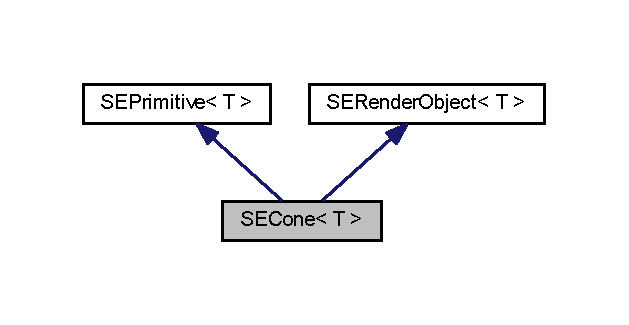
\includegraphics[width=302pt]{class_s_e_cone__inherit__graph}
\end{center}
\end{figure}


Collaboration diagram for S\+E\+Cone$<$ T $>$\+:
\nopagebreak
\begin{figure}[H]
\begin{center}
\leavevmode
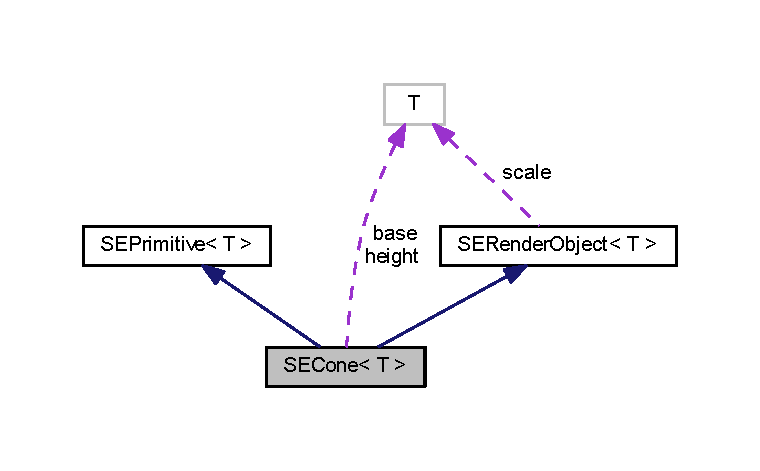
\includegraphics[width=350pt]{class_s_e_cone__coll__graph}
\end{center}
\end{figure}
\subsection*{Public Member Functions}
\begin{DoxyCompactItemize}
\item 
void {\bf set\+Slices} (int sl)
\item 
void {\bf set\+Stacks} (int st)
\item 
void {\bf set\+Base} (T b)
\item 
void {\bf set\+Height} (T h)
\end{DoxyCompactItemize}
\subsection*{Public Attributes}
\begin{DoxyCompactItemize}
\item 
const T \& {\bf base}
\item 
const T \& {\bf height}
\item 
const int \& {\bf slices}
\item 
const int \& {\bf stacks}
\end{DoxyCompactItemize}
\subsection*{Protected Member Functions}
\begin{DoxyCompactItemize}
\item 
{\bf S\+E\+Cone} ()
\item 
{\bf S\+E\+Cone} ({\bf S\+E\+Prim\+Types\+::t\+State} s)
\item 
{\bf S\+E\+Cone} (T b, T h)
\item 
{\bf S\+E\+Cone} (T b, T h, {\bf S\+E\+Prim\+Types\+::t\+State} s)
\item 
virtual {\bf $\sim$\+S\+E\+Cone} ()
\end{DoxyCompactItemize}


\subsection{Detailed Description}
\subsubsection*{template$<$class T$>$class S\+E\+Cone$<$ T $>$}



Definition at line 81 of file S\+E\+Primitive.\+h.



\subsection{Constructor \& Destructor Documentation}
\index{S\+E\+Cone@{S\+E\+Cone}!S\+E\+Cone@{S\+E\+Cone}}
\index{S\+E\+Cone@{S\+E\+Cone}!S\+E\+Cone@{S\+E\+Cone}}
\subsubsection[{S\+E\+Cone}]{\setlength{\rightskip}{0pt plus 5cm}template$<$class T$>$ {\bf S\+E\+Cone}$<$ T $>$\+::{\bf S\+E\+Cone} (
\begin{DoxyParamCaption}
{}
\end{DoxyParamCaption}
)\hspace{0.3cm}{\ttfamily [inline]}, {\ttfamily [protected]}}\label{class_s_e_cone_a6cdea41a994cb15181d1873481954d10}


Definition at line 95 of file S\+E\+Primitive.\+h.

\index{S\+E\+Cone@{S\+E\+Cone}!S\+E\+Cone@{S\+E\+Cone}}
\index{S\+E\+Cone@{S\+E\+Cone}!S\+E\+Cone@{S\+E\+Cone}}
\subsubsection[{S\+E\+Cone}]{\setlength{\rightskip}{0pt plus 5cm}template$<$class T$>$ {\bf S\+E\+Cone}$<$ T $>$\+::{\bf S\+E\+Cone} (
\begin{DoxyParamCaption}
\item[{{\bf S\+E\+Prim\+Types\+::t\+State}}]{s}
\end{DoxyParamCaption}
)\hspace{0.3cm}{\ttfamily [inline]}, {\ttfamily [protected]}}\label{class_s_e_cone_a013d0691b48611aa9a2aec73ac5643b9}


Definition at line 96 of file S\+E\+Primitive.\+h.

\index{S\+E\+Cone@{S\+E\+Cone}!S\+E\+Cone@{S\+E\+Cone}}
\index{S\+E\+Cone@{S\+E\+Cone}!S\+E\+Cone@{S\+E\+Cone}}
\subsubsection[{S\+E\+Cone}]{\setlength{\rightskip}{0pt plus 5cm}template$<$class T$>$ {\bf S\+E\+Cone}$<$ T $>$\+::{\bf S\+E\+Cone} (
\begin{DoxyParamCaption}
\item[{T}]{b, }
\item[{T}]{h}
\end{DoxyParamCaption}
)\hspace{0.3cm}{\ttfamily [inline]}, {\ttfamily [protected]}}\label{class_s_e_cone_a2c4fdad5164f488251c115f8c644d447}


Definition at line 97 of file S\+E\+Primitive.\+h.

\index{S\+E\+Cone@{S\+E\+Cone}!S\+E\+Cone@{S\+E\+Cone}}
\index{S\+E\+Cone@{S\+E\+Cone}!S\+E\+Cone@{S\+E\+Cone}}
\subsubsection[{S\+E\+Cone}]{\setlength{\rightskip}{0pt plus 5cm}template$<$class T$>$ {\bf S\+E\+Cone}$<$ T $>$\+::{\bf S\+E\+Cone} (
\begin{DoxyParamCaption}
\item[{T}]{b, }
\item[{T}]{h, }
\item[{{\bf S\+E\+Prim\+Types\+::t\+State}}]{s}
\end{DoxyParamCaption}
)\hspace{0.3cm}{\ttfamily [inline]}, {\ttfamily [protected]}}\label{class_s_e_cone_a24098784e11bd4ee53f1f5bf4aeeba03}


Definition at line 98 of file S\+E\+Primitive.\+h.

\index{S\+E\+Cone@{S\+E\+Cone}!````~S\+E\+Cone@{$\sim$\+S\+E\+Cone}}
\index{````~S\+E\+Cone@{$\sim$\+S\+E\+Cone}!S\+E\+Cone@{S\+E\+Cone}}
\subsubsection[{$\sim$\+S\+E\+Cone}]{\setlength{\rightskip}{0pt plus 5cm}template$<$class T$>$ virtual {\bf S\+E\+Cone}$<$ T $>$\+::$\sim${\bf S\+E\+Cone} (
\begin{DoxyParamCaption}
{}
\end{DoxyParamCaption}
)\hspace{0.3cm}{\ttfamily [inline]}, {\ttfamily [protected]}, {\ttfamily [virtual]}}\label{class_s_e_cone_a718dea59708bf7249489d0c21d34d8b3}


Definition at line 99 of file S\+E\+Primitive.\+h.



\subsection{Member Function Documentation}
\index{S\+E\+Cone@{S\+E\+Cone}!set\+Base@{set\+Base}}
\index{set\+Base@{set\+Base}!S\+E\+Cone@{S\+E\+Cone}}
\subsubsection[{set\+Base}]{\setlength{\rightskip}{0pt plus 5cm}template$<$class T$>$ void {\bf S\+E\+Cone}$<$ T $>$\+::set\+Base (
\begin{DoxyParamCaption}
\item[{T}]{b}
\end{DoxyParamCaption}
)\hspace{0.3cm}{\ttfamily [inline]}}\label{class_s_e_cone_a2e114b9e03daae0433490a7267e671a4}


Definition at line 91 of file S\+E\+Primitive.\+h.

\index{S\+E\+Cone@{S\+E\+Cone}!set\+Height@{set\+Height}}
\index{set\+Height@{set\+Height}!S\+E\+Cone@{S\+E\+Cone}}
\subsubsection[{set\+Height}]{\setlength{\rightskip}{0pt plus 5cm}template$<$class T$>$ void {\bf S\+E\+Cone}$<$ T $>$\+::set\+Height (
\begin{DoxyParamCaption}
\item[{T}]{h}
\end{DoxyParamCaption}
)\hspace{0.3cm}{\ttfamily [inline]}}\label{class_s_e_cone_ab9630ab324a099c88bafd57a7f2a2d9c}


Definition at line 92 of file S\+E\+Primitive.\+h.

\index{S\+E\+Cone@{S\+E\+Cone}!set\+Slices@{set\+Slices}}
\index{set\+Slices@{set\+Slices}!S\+E\+Cone@{S\+E\+Cone}}
\subsubsection[{set\+Slices}]{\setlength{\rightskip}{0pt plus 5cm}template$<$class T$>$ void {\bf S\+E\+Cone}$<$ T $>$\+::set\+Slices (
\begin{DoxyParamCaption}
\item[{int}]{sl}
\end{DoxyParamCaption}
)\hspace{0.3cm}{\ttfamily [inline]}}\label{class_s_e_cone_ae9af22602853300ede9a8604649aad0f}


Definition at line 89 of file S\+E\+Primitive.\+h.

\index{S\+E\+Cone@{S\+E\+Cone}!set\+Stacks@{set\+Stacks}}
\index{set\+Stacks@{set\+Stacks}!S\+E\+Cone@{S\+E\+Cone}}
\subsubsection[{set\+Stacks}]{\setlength{\rightskip}{0pt plus 5cm}template$<$class T$>$ void {\bf S\+E\+Cone}$<$ T $>$\+::set\+Stacks (
\begin{DoxyParamCaption}
\item[{int}]{st}
\end{DoxyParamCaption}
)\hspace{0.3cm}{\ttfamily [inline]}}\label{class_s_e_cone_a2b113e0bcf274b9c162b5781853f2440}


Definition at line 90 of file S\+E\+Primitive.\+h.



\subsection{Member Data Documentation}
\index{S\+E\+Cone@{S\+E\+Cone}!base@{base}}
\index{base@{base}!S\+E\+Cone@{S\+E\+Cone}}
\subsubsection[{base}]{\setlength{\rightskip}{0pt plus 5cm}template$<$class T$>$ const T\& {\bf S\+E\+Cone}$<$ T $>$\+::base}\label{class_s_e_cone_aeab90a7102aeaa5d1a27e75149e6508d}


Definition at line 84 of file S\+E\+Primitive.\+h.

\index{S\+E\+Cone@{S\+E\+Cone}!height@{height}}
\index{height@{height}!S\+E\+Cone@{S\+E\+Cone}}
\subsubsection[{height}]{\setlength{\rightskip}{0pt plus 5cm}template$<$class T$>$ const T\& {\bf S\+E\+Cone}$<$ T $>$\+::height}\label{class_s_e_cone_a496e02354c29ecdc993b59e7d299cc37}


Definition at line 85 of file S\+E\+Primitive.\+h.

\index{S\+E\+Cone@{S\+E\+Cone}!slices@{slices}}
\index{slices@{slices}!S\+E\+Cone@{S\+E\+Cone}}
\subsubsection[{slices}]{\setlength{\rightskip}{0pt plus 5cm}template$<$class T$>$ const int\& {\bf S\+E\+Cone}$<$ T $>$\+::slices}\label{class_s_e_cone_af328d1f4244868c8950b945152db9ab8}


Definition at line 86 of file S\+E\+Primitive.\+h.

\index{S\+E\+Cone@{S\+E\+Cone}!stacks@{stacks}}
\index{stacks@{stacks}!S\+E\+Cone@{S\+E\+Cone}}
\subsubsection[{stacks}]{\setlength{\rightskip}{0pt plus 5cm}template$<$class T$>$ const int\& {\bf S\+E\+Cone}$<$ T $>$\+::stacks}\label{class_s_e_cone_aa558b39dce639f2ff47ff0db46caf158}


Definition at line 87 of file S\+E\+Primitive.\+h.



The documentation for this class was generated from the following file\+:\begin{DoxyCompactItemize}
\item 
{\bf S\+E\+Primitive.\+h}\end{DoxyCompactItemize}

\section{S\+E\+Configuration\+Loader\+:\+:S\+E\+Config\+Key Union Reference}
\label{union_s_e_configuration_loader_1_1_s_e_config_key}\index{S\+E\+Configuration\+Loader\+::\+S\+E\+Config\+Key@{S\+E\+Configuration\+Loader\+::\+S\+E\+Config\+Key}}


{\ttfamily \#include $<$S\+E\+Configuration\+Loader.\+h$>$}

\subsection*{Public Attributes}
\begin{DoxyCompactItemize}
\item 
int {\bf i}
\item 
float {\bf f}
\item 
double {\bf d}
\item 
char {\bf s} [M\+A\+X\+\_\+\+S\+T\+R\+\_\+\+S\+I\+Z\+E]
\item 
bool {\bf b}
\end{DoxyCompactItemize}


\subsection{Detailed Description}


Definition at line 13 of file S\+E\+Configuration\+Loader.\+h.



\subsection{Member Data Documentation}
\index{S\+E\+Configuration\+Loader\+::\+S\+E\+Config\+Key@{S\+E\+Configuration\+Loader\+::\+S\+E\+Config\+Key}!b@{b}}
\index{b@{b}!S\+E\+Configuration\+Loader\+::\+S\+E\+Config\+Key@{S\+E\+Configuration\+Loader\+::\+S\+E\+Config\+Key}}
\subsubsection[{b}]{\setlength{\rightskip}{0pt plus 5cm}bool S\+E\+Configuration\+Loader\+::\+S\+E\+Config\+Key\+::b}\label{union_s_e_configuration_loader_1_1_s_e_config_key_a430409f997fd6215f209b0b8140065d1}


Definition at line 18 of file S\+E\+Configuration\+Loader.\+h.

\index{S\+E\+Configuration\+Loader\+::\+S\+E\+Config\+Key@{S\+E\+Configuration\+Loader\+::\+S\+E\+Config\+Key}!d@{d}}
\index{d@{d}!S\+E\+Configuration\+Loader\+::\+S\+E\+Config\+Key@{S\+E\+Configuration\+Loader\+::\+S\+E\+Config\+Key}}
\subsubsection[{d}]{\setlength{\rightskip}{0pt plus 5cm}double S\+E\+Configuration\+Loader\+::\+S\+E\+Config\+Key\+::d}\label{union_s_e_configuration_loader_1_1_s_e_config_key_a97f676d38b2e34e86d94462cb37ec687}


Definition at line 16 of file S\+E\+Configuration\+Loader.\+h.

\index{S\+E\+Configuration\+Loader\+::\+S\+E\+Config\+Key@{S\+E\+Configuration\+Loader\+::\+S\+E\+Config\+Key}!f@{f}}
\index{f@{f}!S\+E\+Configuration\+Loader\+::\+S\+E\+Config\+Key@{S\+E\+Configuration\+Loader\+::\+S\+E\+Config\+Key}}
\subsubsection[{f}]{\setlength{\rightskip}{0pt plus 5cm}float S\+E\+Configuration\+Loader\+::\+S\+E\+Config\+Key\+::f}\label{union_s_e_configuration_loader_1_1_s_e_config_key_a053571810a7bb341665fa3ca6c165008}


Definition at line 15 of file S\+E\+Configuration\+Loader.\+h.

\index{S\+E\+Configuration\+Loader\+::\+S\+E\+Config\+Key@{S\+E\+Configuration\+Loader\+::\+S\+E\+Config\+Key}!i@{i}}
\index{i@{i}!S\+E\+Configuration\+Loader\+::\+S\+E\+Config\+Key@{S\+E\+Configuration\+Loader\+::\+S\+E\+Config\+Key}}
\subsubsection[{i}]{\setlength{\rightskip}{0pt plus 5cm}int S\+E\+Configuration\+Loader\+::\+S\+E\+Config\+Key\+::i}\label{union_s_e_configuration_loader_1_1_s_e_config_key_a1c7dd35b903a2fb1c9141938ac780936}


Definition at line 14 of file S\+E\+Configuration\+Loader.\+h.

\index{S\+E\+Configuration\+Loader\+::\+S\+E\+Config\+Key@{S\+E\+Configuration\+Loader\+::\+S\+E\+Config\+Key}!s@{s}}
\index{s@{s}!S\+E\+Configuration\+Loader\+::\+S\+E\+Config\+Key@{S\+E\+Configuration\+Loader\+::\+S\+E\+Config\+Key}}
\subsubsection[{s}]{\setlength{\rightskip}{0pt plus 5cm}char S\+E\+Configuration\+Loader\+::\+S\+E\+Config\+Key\+::s[M\+A\+X\+\_\+\+S\+T\+R\+\_\+\+S\+I\+Z\+E]}\label{union_s_e_configuration_loader_1_1_s_e_config_key_a9d761a4cad424e7e8f6dde55dd44f2c4}


Definition at line 17 of file S\+E\+Configuration\+Loader.\+h.



The documentation for this union was generated from the following file\+:\begin{DoxyCompactItemize}
\item 
{\bf S\+E\+Configuration\+Loader.\+h}\end{DoxyCompactItemize}

\section{S\+E\+Configuration\+Loader Class Reference}
\label{class_s_e_configuration_loader}\index{S\+E\+Configuration\+Loader@{S\+E\+Configuration\+Loader}}


{\ttfamily \#include $<$S\+E\+Configuration\+Loader.\+h$>$}

\subsection*{Classes}
\begin{DoxyCompactItemize}
\item 
union {\bf S\+E\+Config\+Key}
\end{DoxyCompactItemize}
\subsection*{Public Types}
\begin{DoxyCompactItemize}
\item 
typedef std\+::map$<$ const std\+::string, {\bf S\+E\+Config\+Key} $>$ {\bf t\+Keymap}
\end{DoxyCompactItemize}
\subsection*{Public Member Functions}
\begin{DoxyCompactItemize}
\item 
{\bf S\+E\+Configuration\+Loader} ()
\item 
{\bf S\+E\+Configuration\+Loader} (const char $\ast$f)
\item 
{\bf $\sim$\+S\+E\+Configuration\+Loader} ()
\item 
void {\bf load} (const char $\ast$f)
\item 
void {\bf load\+Defaults} ()
\item 
int {\bf get\+Keyi} (std\+::string s)
\item 
float {\bf get\+Keyf} (std\+::string s)
\item 
double {\bf get\+Keyd} (std\+::string s)
\item 
bool {\bf get\+Keyb} (std\+::string s)
\item 
const char $\ast$ {\bf get\+Keyc} (std\+::string s)
\item 
std\+::string {\bf get\+Keys} (std\+::string s)
\end{DoxyCompactItemize}


\subsection{Detailed Description}


Definition at line 7 of file S\+E\+Configuration\+Loader.\+h.



\subsection{Member Typedef Documentation}
\index{S\+E\+Configuration\+Loader@{S\+E\+Configuration\+Loader}!t\+Keymap@{t\+Keymap}}
\index{t\+Keymap@{t\+Keymap}!S\+E\+Configuration\+Loader@{S\+E\+Configuration\+Loader}}
\subsubsection[{t\+Keymap}]{\setlength{\rightskip}{0pt plus 5cm}typedef std\+::map$<$const std\+::string, {\bf S\+E\+Config\+Key}$>$ {\bf S\+E\+Configuration\+Loader\+::t\+Keymap}}\label{class_s_e_configuration_loader_af5be633226adf026a6b5a0c8b9c9eee7}


Definition at line 21 of file S\+E\+Configuration\+Loader.\+h.



\subsection{Constructor \& Destructor Documentation}
\index{S\+E\+Configuration\+Loader@{S\+E\+Configuration\+Loader}!S\+E\+Configuration\+Loader@{S\+E\+Configuration\+Loader}}
\index{S\+E\+Configuration\+Loader@{S\+E\+Configuration\+Loader}!S\+E\+Configuration\+Loader@{S\+E\+Configuration\+Loader}}
\subsubsection[{S\+E\+Configuration\+Loader}]{\setlength{\rightskip}{0pt plus 5cm}S\+E\+Configuration\+Loader\+::\+S\+E\+Configuration\+Loader (
\begin{DoxyParamCaption}
{}
\end{DoxyParamCaption}
)\hspace{0.3cm}{\ttfamily [inline]}}\label{class_s_e_configuration_loader_a9595ec16ed456166f12c222c5b416b91}


Definition at line 28 of file S\+E\+Configuration\+Loader.\+h.



Here is the call graph for this function\+:
\nopagebreak
\begin{figure}[H]
\begin{center}
\leavevmode
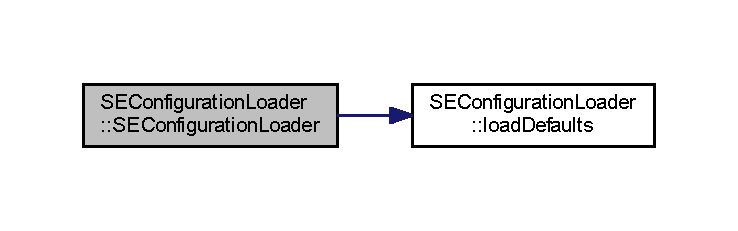
\includegraphics[width=350pt]{class_s_e_configuration_loader_a9595ec16ed456166f12c222c5b416b91_cgraph}
\end{center}
\end{figure}


\index{S\+E\+Configuration\+Loader@{S\+E\+Configuration\+Loader}!S\+E\+Configuration\+Loader@{S\+E\+Configuration\+Loader}}
\index{S\+E\+Configuration\+Loader@{S\+E\+Configuration\+Loader}!S\+E\+Configuration\+Loader@{S\+E\+Configuration\+Loader}}
\subsubsection[{S\+E\+Configuration\+Loader}]{\setlength{\rightskip}{0pt plus 5cm}S\+E\+Configuration\+Loader\+::\+S\+E\+Configuration\+Loader (
\begin{DoxyParamCaption}
\item[{const char $\ast$}]{f}
\end{DoxyParamCaption}
)\hspace{0.3cm}{\ttfamily [inline]}}\label{class_s_e_configuration_loader_a3bbbe0a39d3d09d77e5605fece80693d}


Definition at line 29 of file S\+E\+Configuration\+Loader.\+h.



Here is the call graph for this function\+:
\nopagebreak
\begin{figure}[H]
\begin{center}
\leavevmode
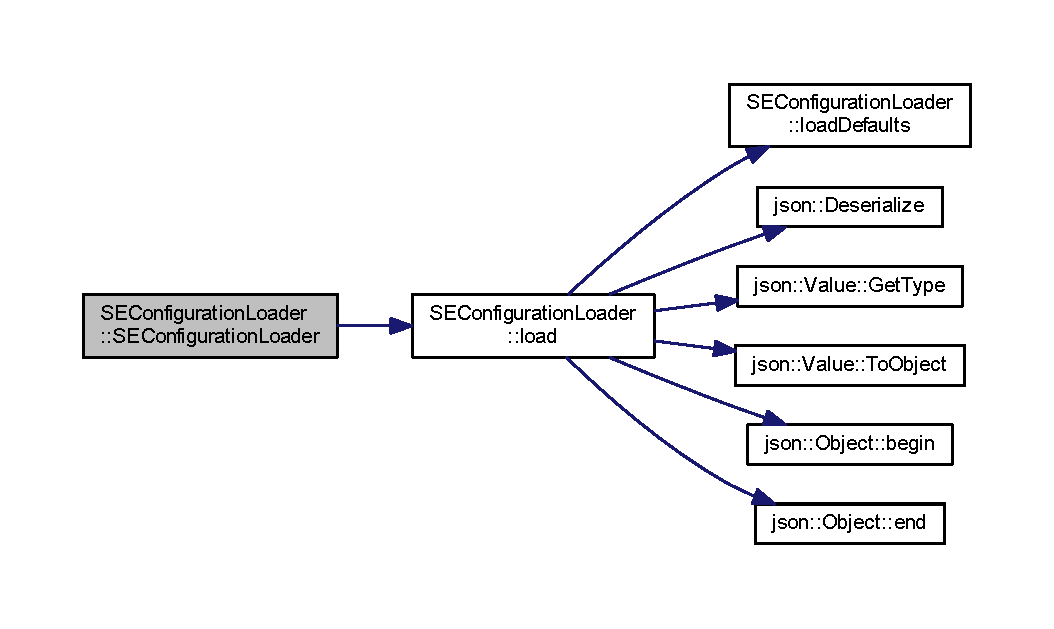
\includegraphics[width=350pt]{class_s_e_configuration_loader_a3bbbe0a39d3d09d77e5605fece80693d_cgraph}
\end{center}
\end{figure}


\index{S\+E\+Configuration\+Loader@{S\+E\+Configuration\+Loader}!````~S\+E\+Configuration\+Loader@{$\sim$\+S\+E\+Configuration\+Loader}}
\index{````~S\+E\+Configuration\+Loader@{$\sim$\+S\+E\+Configuration\+Loader}!S\+E\+Configuration\+Loader@{S\+E\+Configuration\+Loader}}
\subsubsection[{$\sim$\+S\+E\+Configuration\+Loader}]{\setlength{\rightskip}{0pt plus 5cm}S\+E\+Configuration\+Loader\+::$\sim$\+S\+E\+Configuration\+Loader (
\begin{DoxyParamCaption}
{}
\end{DoxyParamCaption}
)\hspace{0.3cm}{\ttfamily [inline]}}\label{class_s_e_configuration_loader_a21d9070872b6d086fddc1cf19700f203}


Definition at line 30 of file S\+E\+Configuration\+Loader.\+h.



\subsection{Member Function Documentation}
\index{S\+E\+Configuration\+Loader@{S\+E\+Configuration\+Loader}!get\+Keyb@{get\+Keyb}}
\index{get\+Keyb@{get\+Keyb}!S\+E\+Configuration\+Loader@{S\+E\+Configuration\+Loader}}
\subsubsection[{get\+Keyb}]{\setlength{\rightskip}{0pt plus 5cm}bool S\+E\+Configuration\+Loader\+::get\+Keyb (
\begin{DoxyParamCaption}
\item[{std\+::string}]{s}
\end{DoxyParamCaption}
)\hspace{0.3cm}{\ttfamily [inline]}}\label{class_s_e_configuration_loader_aa157af98bba8e31dd53586e9585ff80a}


Definition at line 38 of file S\+E\+Configuration\+Loader.\+h.

\index{S\+E\+Configuration\+Loader@{S\+E\+Configuration\+Loader}!get\+Keyc@{get\+Keyc}}
\index{get\+Keyc@{get\+Keyc}!S\+E\+Configuration\+Loader@{S\+E\+Configuration\+Loader}}
\subsubsection[{get\+Keyc}]{\setlength{\rightskip}{0pt plus 5cm}const char$\ast$ S\+E\+Configuration\+Loader\+::get\+Keyc (
\begin{DoxyParamCaption}
\item[{std\+::string}]{s}
\end{DoxyParamCaption}
)\hspace{0.3cm}{\ttfamily [inline]}}\label{class_s_e_configuration_loader_a622c37165b5599702345042da335246d}


Definition at line 39 of file S\+E\+Configuration\+Loader.\+h.

\index{S\+E\+Configuration\+Loader@{S\+E\+Configuration\+Loader}!get\+Keyd@{get\+Keyd}}
\index{get\+Keyd@{get\+Keyd}!S\+E\+Configuration\+Loader@{S\+E\+Configuration\+Loader}}
\subsubsection[{get\+Keyd}]{\setlength{\rightskip}{0pt plus 5cm}double S\+E\+Configuration\+Loader\+::get\+Keyd (
\begin{DoxyParamCaption}
\item[{std\+::string}]{s}
\end{DoxyParamCaption}
)\hspace{0.3cm}{\ttfamily [inline]}}\label{class_s_e_configuration_loader_a40e4daf97e031981a2a38dd94c1ff3e7}


Definition at line 37 of file S\+E\+Configuration\+Loader.\+h.

\index{S\+E\+Configuration\+Loader@{S\+E\+Configuration\+Loader}!get\+Keyf@{get\+Keyf}}
\index{get\+Keyf@{get\+Keyf}!S\+E\+Configuration\+Loader@{S\+E\+Configuration\+Loader}}
\subsubsection[{get\+Keyf}]{\setlength{\rightskip}{0pt plus 5cm}float S\+E\+Configuration\+Loader\+::get\+Keyf (
\begin{DoxyParamCaption}
\item[{std\+::string}]{s}
\end{DoxyParamCaption}
)\hspace{0.3cm}{\ttfamily [inline]}}\label{class_s_e_configuration_loader_a01c7a531d58a9555aa0cdab32b7ae229}


Definition at line 36 of file S\+E\+Configuration\+Loader.\+h.

\index{S\+E\+Configuration\+Loader@{S\+E\+Configuration\+Loader}!get\+Keyi@{get\+Keyi}}
\index{get\+Keyi@{get\+Keyi}!S\+E\+Configuration\+Loader@{S\+E\+Configuration\+Loader}}
\subsubsection[{get\+Keyi}]{\setlength{\rightskip}{0pt plus 5cm}int S\+E\+Configuration\+Loader\+::get\+Keyi (
\begin{DoxyParamCaption}
\item[{std\+::string}]{s}
\end{DoxyParamCaption}
)\hspace{0.3cm}{\ttfamily [inline]}}\label{class_s_e_configuration_loader_a74815def251ae7db28763a562ff820c3}


Definition at line 35 of file S\+E\+Configuration\+Loader.\+h.

\index{S\+E\+Configuration\+Loader@{S\+E\+Configuration\+Loader}!get\+Keys@{get\+Keys}}
\index{get\+Keys@{get\+Keys}!S\+E\+Configuration\+Loader@{S\+E\+Configuration\+Loader}}
\subsubsection[{get\+Keys}]{\setlength{\rightskip}{0pt plus 5cm}std\+::string S\+E\+Configuration\+Loader\+::get\+Keys (
\begin{DoxyParamCaption}
\item[{std\+::string}]{s}
\end{DoxyParamCaption}
)\hspace{0.3cm}{\ttfamily [inline]}}\label{class_s_e_configuration_loader_a77371959f3b87be3ef65668e64351d63}


Definition at line 40 of file S\+E\+Configuration\+Loader.\+h.

\index{S\+E\+Configuration\+Loader@{S\+E\+Configuration\+Loader}!load@{load}}
\index{load@{load}!S\+E\+Configuration\+Loader@{S\+E\+Configuration\+Loader}}
\subsubsection[{load}]{\setlength{\rightskip}{0pt plus 5cm}void S\+E\+Configuration\+Loader\+::load (
\begin{DoxyParamCaption}
\item[{const char $\ast$}]{f}
\end{DoxyParamCaption}
)}\label{class_s_e_configuration_loader_a78863f73bf309faf2a8b9054e61c7efe}


Definition at line 6 of file S\+E\+Configuration\+Loader.\+cpp.



Here is the call graph for this function\+:
\nopagebreak
\begin{figure}[H]
\begin{center}
\leavevmode
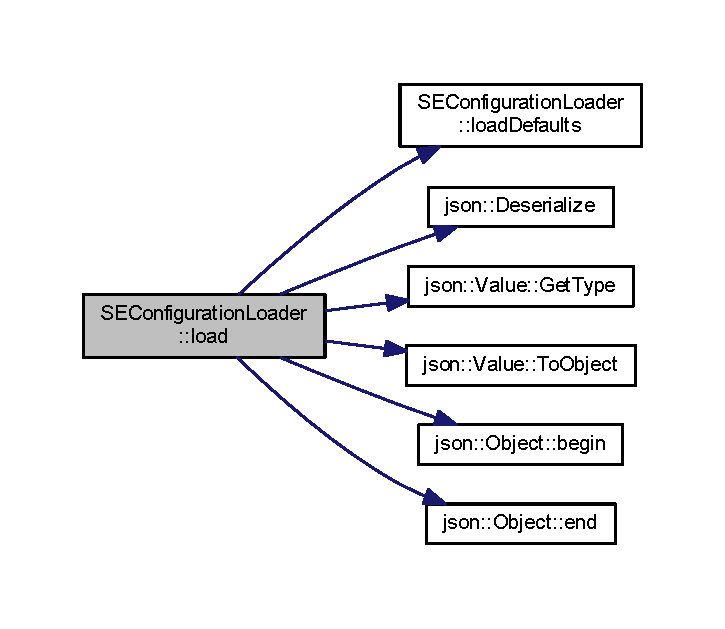
\includegraphics[width=348pt]{class_s_e_configuration_loader_a78863f73bf309faf2a8b9054e61c7efe_cgraph}
\end{center}
\end{figure}


\index{S\+E\+Configuration\+Loader@{S\+E\+Configuration\+Loader}!load\+Defaults@{load\+Defaults}}
\index{load\+Defaults@{load\+Defaults}!S\+E\+Configuration\+Loader@{S\+E\+Configuration\+Loader}}
\subsubsection[{load\+Defaults}]{\setlength{\rightskip}{0pt plus 5cm}void S\+E\+Configuration\+Loader\+::load\+Defaults (
\begin{DoxyParamCaption}
{}
\end{DoxyParamCaption}
)}\label{class_s_e_configuration_loader_ad2dcb8cb7d6f36eff70013a4ee9db216}


Definition at line 51 of file S\+E\+Configuration\+Loader.\+cpp.



The documentation for this class was generated from the following files\+:\begin{DoxyCompactItemize}
\item 
{\bf S\+E\+Configuration\+Loader.\+h}\item 
{\bf S\+E\+Configuration\+Loader.\+cpp}\end{DoxyCompactItemize}

\section{S\+E\+Cube$<$ T $>$ Class Template Reference}
\label{class_s_e_cube}\index{S\+E\+Cube$<$ T $>$@{S\+E\+Cube$<$ T $>$}}


{\ttfamily \#include $<$S\+E\+Primitive.\+h$>$}



Inheritance diagram for S\+E\+Cube$<$ T $>$\+:
\nopagebreak
\begin{figure}[H]
\begin{center}
\leavevmode
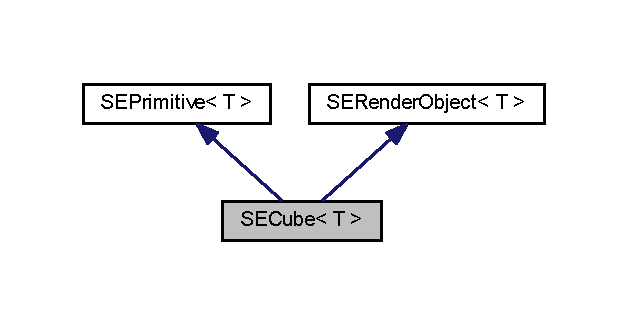
\includegraphics[width=302pt]{class_s_e_cube__inherit__graph}
\end{center}
\end{figure}


Collaboration diagram for S\+E\+Cube$<$ T $>$\+:
\nopagebreak
\begin{figure}[H]
\begin{center}
\leavevmode
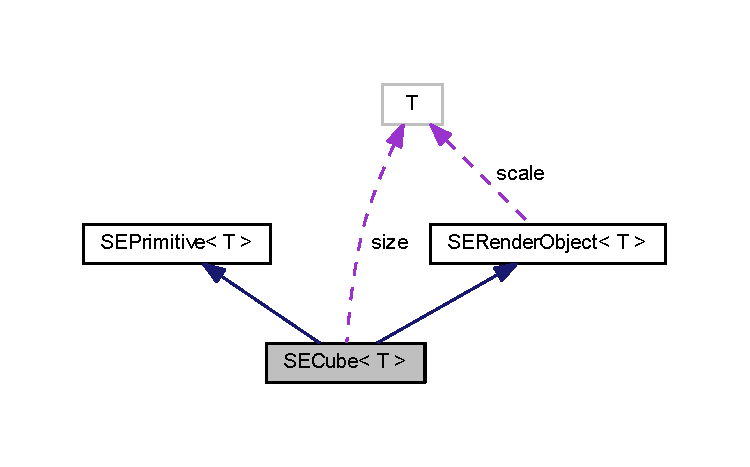
\includegraphics[width=350pt]{class_s_e_cube__coll__graph}
\end{center}
\end{figure}
\subsection*{Public Member Functions}
\begin{DoxyCompactItemize}
\item 
void {\bf set\+Size} (T s)
\end{DoxyCompactItemize}
\subsection*{Public Attributes}
\begin{DoxyCompactItemize}
\item 
const T \& {\bf size}
\end{DoxyCompactItemize}
\subsection*{Protected Member Functions}
\begin{DoxyCompactItemize}
\item 
{\bf S\+E\+Cube} ()
\item 
{\bf S\+E\+Cube} ({\bf S\+E\+Prim\+Types\+::t\+State} st)
\item 
{\bf S\+E\+Cube} (T sz)
\item 
{\bf S\+E\+Cube} (T sz, {\bf S\+E\+Prim\+Types\+::t\+State} st)
\item 
virtual {\bf $\sim$\+S\+E\+Cube} ()
\end{DoxyCompactItemize}


\subsection{Detailed Description}
\subsubsection*{template$<$class T$>$class S\+E\+Cube$<$ T $>$}



Definition at line 63 of file S\+E\+Primitive.\+h.



\subsection{Constructor \& Destructor Documentation}
\index{S\+E\+Cube@{S\+E\+Cube}!S\+E\+Cube@{S\+E\+Cube}}
\index{S\+E\+Cube@{S\+E\+Cube}!S\+E\+Cube@{S\+E\+Cube}}
\subsubsection[{S\+E\+Cube}]{\setlength{\rightskip}{0pt plus 5cm}template$<$class T$>$ {\bf S\+E\+Cube}$<$ T $>$\+::{\bf S\+E\+Cube} (
\begin{DoxyParamCaption}
{}
\end{DoxyParamCaption}
)\hspace{0.3cm}{\ttfamily [inline]}, {\ttfamily [protected]}}\label{class_s_e_cube_a85fa6046163acccd062b492f346e7e78}


Definition at line 71 of file S\+E\+Primitive.\+h.

\index{S\+E\+Cube@{S\+E\+Cube}!S\+E\+Cube@{S\+E\+Cube}}
\index{S\+E\+Cube@{S\+E\+Cube}!S\+E\+Cube@{S\+E\+Cube}}
\subsubsection[{S\+E\+Cube}]{\setlength{\rightskip}{0pt plus 5cm}template$<$class T$>$ {\bf S\+E\+Cube}$<$ T $>$\+::{\bf S\+E\+Cube} (
\begin{DoxyParamCaption}
\item[{{\bf S\+E\+Prim\+Types\+::t\+State}}]{st}
\end{DoxyParamCaption}
)\hspace{0.3cm}{\ttfamily [inline]}, {\ttfamily [protected]}}\label{class_s_e_cube_a54358093c29312c0e86d294b256f7444}


Definition at line 72 of file S\+E\+Primitive.\+h.

\index{S\+E\+Cube@{S\+E\+Cube}!S\+E\+Cube@{S\+E\+Cube}}
\index{S\+E\+Cube@{S\+E\+Cube}!S\+E\+Cube@{S\+E\+Cube}}
\subsubsection[{S\+E\+Cube}]{\setlength{\rightskip}{0pt plus 5cm}template$<$class T$>$ {\bf S\+E\+Cube}$<$ T $>$\+::{\bf S\+E\+Cube} (
\begin{DoxyParamCaption}
\item[{T}]{sz}
\end{DoxyParamCaption}
)\hspace{0.3cm}{\ttfamily [inline]}, {\ttfamily [protected]}}\label{class_s_e_cube_a050a405992f0e3217d6874d0af967920}


Definition at line 73 of file S\+E\+Primitive.\+h.

\index{S\+E\+Cube@{S\+E\+Cube}!S\+E\+Cube@{S\+E\+Cube}}
\index{S\+E\+Cube@{S\+E\+Cube}!S\+E\+Cube@{S\+E\+Cube}}
\subsubsection[{S\+E\+Cube}]{\setlength{\rightskip}{0pt plus 5cm}template$<$class T$>$ {\bf S\+E\+Cube}$<$ T $>$\+::{\bf S\+E\+Cube} (
\begin{DoxyParamCaption}
\item[{T}]{sz, }
\item[{{\bf S\+E\+Prim\+Types\+::t\+State}}]{st}
\end{DoxyParamCaption}
)\hspace{0.3cm}{\ttfamily [inline]}, {\ttfamily [protected]}}\label{class_s_e_cube_a25a171071f0483eb5c8dc71597f262ba}


Definition at line 74 of file S\+E\+Primitive.\+h.

\index{S\+E\+Cube@{S\+E\+Cube}!````~S\+E\+Cube@{$\sim$\+S\+E\+Cube}}
\index{````~S\+E\+Cube@{$\sim$\+S\+E\+Cube}!S\+E\+Cube@{S\+E\+Cube}}
\subsubsection[{$\sim$\+S\+E\+Cube}]{\setlength{\rightskip}{0pt plus 5cm}template$<$class T$>$ virtual {\bf S\+E\+Cube}$<$ T $>$\+::$\sim${\bf S\+E\+Cube} (
\begin{DoxyParamCaption}
{}
\end{DoxyParamCaption}
)\hspace{0.3cm}{\ttfamily [inline]}, {\ttfamily [protected]}, {\ttfamily [virtual]}}\label{class_s_e_cube_ae7168559fefc574ef4300caabaf36ccd}


Definition at line 75 of file S\+E\+Primitive.\+h.



\subsection{Member Function Documentation}
\index{S\+E\+Cube@{S\+E\+Cube}!set\+Size@{set\+Size}}
\index{set\+Size@{set\+Size}!S\+E\+Cube@{S\+E\+Cube}}
\subsubsection[{set\+Size}]{\setlength{\rightskip}{0pt plus 5cm}template$<$class T$>$ void {\bf S\+E\+Cube}$<$ T $>$\+::set\+Size (
\begin{DoxyParamCaption}
\item[{T}]{s}
\end{DoxyParamCaption}
)\hspace{0.3cm}{\ttfamily [inline]}}\label{class_s_e_cube_a3c4546cfb077c391151cb21e0187bb7a}


Definition at line 68 of file S\+E\+Primitive.\+h.



\subsection{Member Data Documentation}
\index{S\+E\+Cube@{S\+E\+Cube}!size@{size}}
\index{size@{size}!S\+E\+Cube@{S\+E\+Cube}}
\subsubsection[{size}]{\setlength{\rightskip}{0pt plus 5cm}template$<$class T$>$ const T\& {\bf S\+E\+Cube}$<$ T $>$\+::size}\label{class_s_e_cube_ab726c27d2273bb515c7445d1395cc021}


Definition at line 66 of file S\+E\+Primitive.\+h.



The documentation for this class was generated from the following file\+:\begin{DoxyCompactItemize}
\item 
{\bf S\+E\+Primitive.\+h}\end{DoxyCompactItemize}

\section{S\+E\+Directional\+Light$<$ T $>$ Class Template Reference}
\label{class_s_e_directional_light}\index{S\+E\+Directional\+Light$<$ T $>$@{S\+E\+Directional\+Light$<$ T $>$}}


{\ttfamily \#include $<$S\+E\+Light.\+h$>$}



Inheritance diagram for S\+E\+Directional\+Light$<$ T $>$\+:
\nopagebreak
\begin{figure}[H]
\begin{center}
\leavevmode
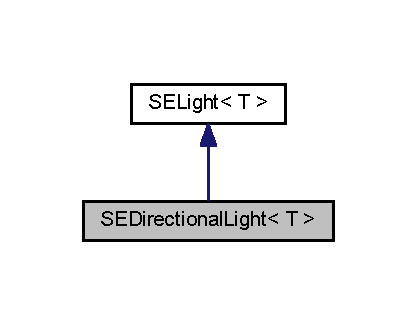
\includegraphics[width=200pt]{class_s_e_directional_light__inherit__graph}
\end{center}
\end{figure}


Collaboration diagram for S\+E\+Directional\+Light$<$ T $>$\+:
\nopagebreak
\begin{figure}[H]
\begin{center}
\leavevmode
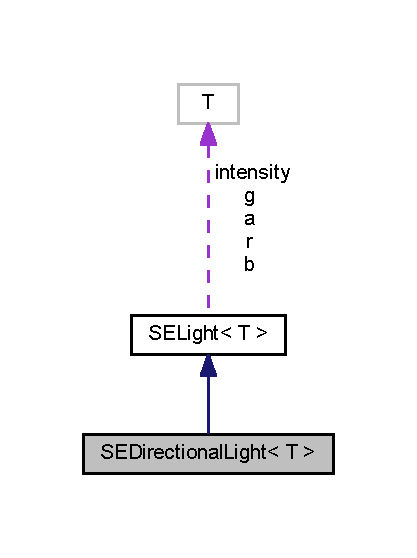
\includegraphics[width=200pt]{class_s_e_directional_light__coll__graph}
\end{center}
\end{figure}
\subsection*{Public Member Functions}
\begin{DoxyCompactItemize}
\item 
virtual {\bf S\+E\+Directional\+Light}$<$ T $>$ \& {\bf set\+Direction} ({\bf S\+E\+Vec3}$<$ T $>$ d)
\item 
virtual {\bf S\+E\+Directional\+Light}$<$ T $>$ \& {\bf set\+Direction} (T x, T y, T z)
\end{DoxyCompactItemize}
\subsection*{Public Attributes}
\begin{DoxyCompactItemize}
\item 
const {\bf S\+E\+Vec4}$<$ T $>$ \& {\bf direction}
\end{DoxyCompactItemize}
\subsection*{Protected Member Functions}
\begin{DoxyCompactItemize}
\item 
{\bf S\+E\+Directional\+Light} ()
\item 
{\bf S\+E\+Directional\+Light} (T {\bf r}, T {\bf g}, T {\bf b}, T {\bf a})
\item 
virtual {\bf $\sim$\+S\+E\+Directional\+Light} ()
\end{DoxyCompactItemize}


\subsection{Detailed Description}
\subsubsection*{template$<$class T$>$class S\+E\+Directional\+Light$<$ T $>$}



Definition at line 96 of file S\+E\+Light.\+h.



\subsection{Constructor \& Destructor Documentation}
\index{S\+E\+Directional\+Light@{S\+E\+Directional\+Light}!S\+E\+Directional\+Light@{S\+E\+Directional\+Light}}
\index{S\+E\+Directional\+Light@{S\+E\+Directional\+Light}!S\+E\+Directional\+Light@{S\+E\+Directional\+Light}}
\subsubsection[{S\+E\+Directional\+Light}]{\setlength{\rightskip}{0pt plus 5cm}template$<$class T$>$ {\bf S\+E\+Directional\+Light}$<$ T $>$\+::{\bf S\+E\+Directional\+Light} (
\begin{DoxyParamCaption}
{}
\end{DoxyParamCaption}
)\hspace{0.3cm}{\ttfamily [inline]}, {\ttfamily [protected]}}\label{class_s_e_directional_light_a27541326fa3fe526575a72846e995b31}


Definition at line 105 of file S\+E\+Light.\+h.

\index{S\+E\+Directional\+Light@{S\+E\+Directional\+Light}!S\+E\+Directional\+Light@{S\+E\+Directional\+Light}}
\index{S\+E\+Directional\+Light@{S\+E\+Directional\+Light}!S\+E\+Directional\+Light@{S\+E\+Directional\+Light}}
\subsubsection[{S\+E\+Directional\+Light}]{\setlength{\rightskip}{0pt plus 5cm}template$<$class T$>$ {\bf S\+E\+Directional\+Light}$<$ T $>$\+::{\bf S\+E\+Directional\+Light} (
\begin{DoxyParamCaption}
\item[{T}]{r, }
\item[{T}]{g, }
\item[{T}]{b, }
\item[{T}]{a}
\end{DoxyParamCaption}
)\hspace{0.3cm}{\ttfamily [inline]}, {\ttfamily [protected]}}\label{class_s_e_directional_light_a2a273a03636946bd55bbe34e1798c0d6}


Definition at line 106 of file S\+E\+Light.\+h.

\index{S\+E\+Directional\+Light@{S\+E\+Directional\+Light}!````~S\+E\+Directional\+Light@{$\sim$\+S\+E\+Directional\+Light}}
\index{````~S\+E\+Directional\+Light@{$\sim$\+S\+E\+Directional\+Light}!S\+E\+Directional\+Light@{S\+E\+Directional\+Light}}
\subsubsection[{$\sim$\+S\+E\+Directional\+Light}]{\setlength{\rightskip}{0pt plus 5cm}template$<$class T$>$ virtual {\bf S\+E\+Directional\+Light}$<$ T $>$\+::$\sim${\bf S\+E\+Directional\+Light} (
\begin{DoxyParamCaption}
{}
\end{DoxyParamCaption}
)\hspace{0.3cm}{\ttfamily [inline]}, {\ttfamily [protected]}, {\ttfamily [virtual]}}\label{class_s_e_directional_light_af0d3cd363fe0f4a3af4d9f37ad2cac0e}


Definition at line 107 of file S\+E\+Light.\+h.



\subsection{Member Function Documentation}
\index{S\+E\+Directional\+Light@{S\+E\+Directional\+Light}!set\+Direction@{set\+Direction}}
\index{set\+Direction@{set\+Direction}!S\+E\+Directional\+Light@{S\+E\+Directional\+Light}}
\subsubsection[{set\+Direction}]{\setlength{\rightskip}{0pt plus 5cm}template$<$class T$>$ virtual {\bf S\+E\+Directional\+Light}$<$T$>$\& {\bf S\+E\+Directional\+Light}$<$ T $>$\+::set\+Direction (
\begin{DoxyParamCaption}
\item[{{\bf S\+E\+Vec3}$<$ T $>$}]{d}
\end{DoxyParamCaption}
)\hspace{0.3cm}{\ttfamily [inline]}, {\ttfamily [virtual]}}\label{class_s_e_directional_light_ac6baccbe8eeef19e26de690b8e349c4d}


Definition at line 101 of file S\+E\+Light.\+h.

\index{S\+E\+Directional\+Light@{S\+E\+Directional\+Light}!set\+Direction@{set\+Direction}}
\index{set\+Direction@{set\+Direction}!S\+E\+Directional\+Light@{S\+E\+Directional\+Light}}
\subsubsection[{set\+Direction}]{\setlength{\rightskip}{0pt plus 5cm}template$<$class T$>$ virtual {\bf S\+E\+Directional\+Light}$<$T$>$\& {\bf S\+E\+Directional\+Light}$<$ T $>$\+::set\+Direction (
\begin{DoxyParamCaption}
\item[{T}]{x, }
\item[{T}]{y, }
\item[{T}]{z}
\end{DoxyParamCaption}
)\hspace{0.3cm}{\ttfamily [inline]}, {\ttfamily [virtual]}}\label{class_s_e_directional_light_a43b5241078707653f009fea408f886c9}


Definition at line 102 of file S\+E\+Light.\+h.



\subsection{Member Data Documentation}
\index{S\+E\+Directional\+Light@{S\+E\+Directional\+Light}!direction@{direction}}
\index{direction@{direction}!S\+E\+Directional\+Light@{S\+E\+Directional\+Light}}
\subsubsection[{direction}]{\setlength{\rightskip}{0pt plus 5cm}template$<$class T$>$ const {\bf S\+E\+Vec4}$<$T$>$\& {\bf S\+E\+Directional\+Light}$<$ T $>$\+::direction}\label{class_s_e_directional_light_a2454d3ab0e43066d8e387ef13b7e27e3}


Definition at line 99 of file S\+E\+Light.\+h.



The documentation for this class was generated from the following file\+:\begin{DoxyCompactItemize}
\item 
{\bf S\+E\+Light.\+h}\end{DoxyCompactItemize}

\section{S\+E\+Entity Class Reference}
\label{class_s_e_entity}\index{S\+E\+Entity@{S\+E\+Entity}}


{\ttfamily \#include $<$S\+E\+Entity.\+h$>$}



Inheritance diagram for S\+E\+Entity\+:
\nopagebreak
\begin{figure}[H]
\begin{center}
\leavevmode
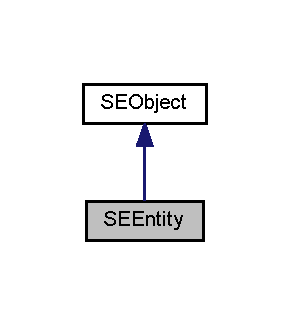
\includegraphics[width=139pt]{class_s_e_entity__inherit__graph}
\end{center}
\end{figure}


Collaboration diagram for S\+E\+Entity\+:
\nopagebreak
\begin{figure}[H]
\begin{center}
\leavevmode
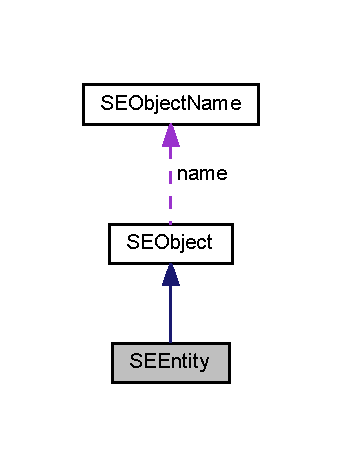
\includegraphics[width=164pt]{class_s_e_entity__coll__graph}
\end{center}
\end{figure}
\subsection*{Public Member Functions}
\begin{DoxyCompactItemize}
\item 
{\bf S\+E\+Entity} ()
\item 
{\bf S\+E\+Entity} (const std\+::string \&n)
\item 
{\bf $\sim$\+S\+E\+Entity} ()
\item 
virtual void {\bf update} (double dt)
\item 
bool {\bf query\+Component} ({\bf S\+E\+Component\+::t\+Component} c)
\item 
void {\bf register\+Component} ({\bf S\+E\+Component} $\ast$c)
\item 
{\bf S\+E\+Component} $\ast$ {\bf get\+Component} ({\bf S\+E\+Component\+::t\+Component} t)
\end{DoxyCompactItemize}
\subsection*{Additional Inherited Members}


\subsection{Detailed Description}


Definition at line 10 of file S\+E\+Entity.\+h.



\subsection{Constructor \& Destructor Documentation}
\index{S\+E\+Entity@{S\+E\+Entity}!S\+E\+Entity@{S\+E\+Entity}}
\index{S\+E\+Entity@{S\+E\+Entity}!S\+E\+Entity@{S\+E\+Entity}}
\subsubsection[{S\+E\+Entity}]{\setlength{\rightskip}{0pt plus 5cm}S\+E\+Entity\+::\+S\+E\+Entity (
\begin{DoxyParamCaption}
{}
\end{DoxyParamCaption}
)\hspace{0.3cm}{\ttfamily [inline]}}\label{class_s_e_entity_ab5fa9f3568b1ce1d7f678b70ffd5c5d5}


Definition at line 13 of file S\+E\+Entity.\+h.

\index{S\+E\+Entity@{S\+E\+Entity}!S\+E\+Entity@{S\+E\+Entity}}
\index{S\+E\+Entity@{S\+E\+Entity}!S\+E\+Entity@{S\+E\+Entity}}
\subsubsection[{S\+E\+Entity}]{\setlength{\rightskip}{0pt plus 5cm}S\+E\+Entity\+::\+S\+E\+Entity (
\begin{DoxyParamCaption}
\item[{const std\+::string \&}]{n}
\end{DoxyParamCaption}
)\hspace{0.3cm}{\ttfamily [inline]}}\label{class_s_e_entity_ad92c9eb458bb65fe4eeb9b45a1c02aa3}


Definition at line 14 of file S\+E\+Entity.\+h.

\index{S\+E\+Entity@{S\+E\+Entity}!````~S\+E\+Entity@{$\sim$\+S\+E\+Entity}}
\index{````~S\+E\+Entity@{$\sim$\+S\+E\+Entity}!S\+E\+Entity@{S\+E\+Entity}}
\subsubsection[{$\sim$\+S\+E\+Entity}]{\setlength{\rightskip}{0pt plus 5cm}S\+E\+Entity\+::$\sim$\+S\+E\+Entity (
\begin{DoxyParamCaption}
{}
\end{DoxyParamCaption}
)\hspace{0.3cm}{\ttfamily [inline]}}\label{class_s_e_entity_a7aeeb3e6a063adb6807b0a2bd05be676}


Definition at line 15 of file S\+E\+Entity.\+h.



\subsection{Member Function Documentation}
\index{S\+E\+Entity@{S\+E\+Entity}!get\+Component@{get\+Component}}
\index{get\+Component@{get\+Component}!S\+E\+Entity@{S\+E\+Entity}}
\subsubsection[{get\+Component}]{\setlength{\rightskip}{0pt plus 5cm}{\bf S\+E\+Component}$\ast$ S\+E\+Entity\+::get\+Component (
\begin{DoxyParamCaption}
\item[{{\bf S\+E\+Component\+::t\+Component}}]{t}
\end{DoxyParamCaption}
)\hspace{0.3cm}{\ttfamily [inline]}}\label{class_s_e_entity_aceac00651d84253a224c903bcd5e8fd0}


Definition at line 22 of file S\+E\+Entity.\+h.

\index{S\+E\+Entity@{S\+E\+Entity}!query\+Component@{query\+Component}}
\index{query\+Component@{query\+Component}!S\+E\+Entity@{S\+E\+Entity}}
\subsubsection[{query\+Component}]{\setlength{\rightskip}{0pt plus 5cm}bool S\+E\+Entity\+::query\+Component (
\begin{DoxyParamCaption}
\item[{{\bf S\+E\+Component\+::t\+Component}}]{c}
\end{DoxyParamCaption}
)\hspace{0.3cm}{\ttfamily [inline]}}\label{class_s_e_entity_a80f53a36635a83da071453a4db0de8e5}


Definition at line 19 of file S\+E\+Entity.\+h.

\index{S\+E\+Entity@{S\+E\+Entity}!register\+Component@{register\+Component}}
\index{register\+Component@{register\+Component}!S\+E\+Entity@{S\+E\+Entity}}
\subsubsection[{register\+Component}]{\setlength{\rightskip}{0pt plus 5cm}void S\+E\+Entity\+::register\+Component (
\begin{DoxyParamCaption}
\item[{{\bf S\+E\+Component} $\ast$}]{c}
\end{DoxyParamCaption}
)\hspace{0.3cm}{\ttfamily [inline]}}\label{class_s_e_entity_a4b2b357f83cee39bfa38130a5e72d81e}


Definition at line 21 of file S\+E\+Entity.\+h.



Here is the call graph for this function\+:
\nopagebreak
\begin{figure}[H]
\begin{center}
\leavevmode
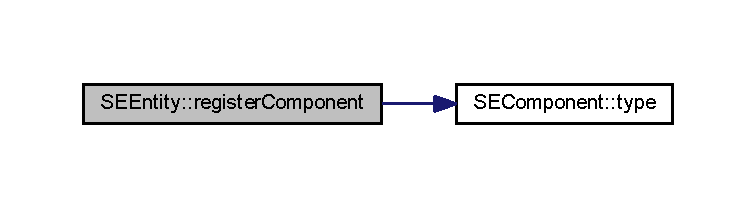
\includegraphics[width=350pt]{class_s_e_entity_a4b2b357f83cee39bfa38130a5e72d81e_cgraph}
\end{center}
\end{figure}


\index{S\+E\+Entity@{S\+E\+Entity}!update@{update}}
\index{update@{update}!S\+E\+Entity@{S\+E\+Entity}}
\subsubsection[{update}]{\setlength{\rightskip}{0pt plus 5cm}virtual void S\+E\+Entity\+::update (
\begin{DoxyParamCaption}
\item[{double}]{dt}
\end{DoxyParamCaption}
)\hspace{0.3cm}{\ttfamily [inline]}, {\ttfamily [virtual]}}\label{class_s_e_entity_a0e1247a2c7bbd2de943cef5d18ac1ed8}


Definition at line 17 of file S\+E\+Entity.\+h.



The documentation for this class was generated from the following file\+:\begin{DoxyCompactItemize}
\item 
{\bf S\+E\+Entity.\+h}\end{DoxyCompactItemize}

\section{S\+E\+Event\+Handler Class Reference}
\label{class_s_e_event_handler}\index{S\+E\+Event\+Handler@{S\+E\+Event\+Handler}}


{\ttfamily \#include $<$S\+E\+Event\+Handler.\+h$>$}

\subsection*{Public Types}
\begin{DoxyCompactItemize}
\item 
enum {\bf t\+Event\+Handler} \{ {\bf G\+L\+U\+I\+\_\+\+E\+H}, 
{\bf G\+L\+U\+T\+\_\+\+E\+H}, 
{\bf N\+U\+M\+\_\+\+E\+H\+S}
 \}
\end{DoxyCompactItemize}


\subsection{Detailed Description}


Definition at line 4 of file S\+E\+Event\+Handler.\+h.



\subsection{Member Enumeration Documentation}
\index{S\+E\+Event\+Handler@{S\+E\+Event\+Handler}!t\+Event\+Handler@{t\+Event\+Handler}}
\index{t\+Event\+Handler@{t\+Event\+Handler}!S\+E\+Event\+Handler@{S\+E\+Event\+Handler}}
\subsubsection[{t\+Event\+Handler}]{\setlength{\rightskip}{0pt plus 5cm}enum {\bf S\+E\+Event\+Handler\+::t\+Event\+Handler}}\label{class_s_e_event_handler_ab9bab28bd45f28d90cefc484ec4c6b84}
\begin{Desc}
\item[Enumerator]\par
\begin{description}
\index{G\+L\+U\+I\+\_\+\+E\+H@{G\+L\+U\+I\+\_\+\+E\+H}!S\+E\+Event\+Handler@{S\+E\+Event\+Handler}}\index{S\+E\+Event\+Handler@{S\+E\+Event\+Handler}!G\+L\+U\+I\+\_\+\+E\+H@{G\+L\+U\+I\+\_\+\+E\+H}}\item[{\em 
G\+L\+U\+I\+\_\+\+E\+H\label{class_s_e_event_handler_ab9bab28bd45f28d90cefc484ec4c6b84a7feb56baca46cda5fe8743701fe9bcf5}
}]\index{G\+L\+U\+T\+\_\+\+E\+H@{G\+L\+U\+T\+\_\+\+E\+H}!S\+E\+Event\+Handler@{S\+E\+Event\+Handler}}\index{S\+E\+Event\+Handler@{S\+E\+Event\+Handler}!G\+L\+U\+T\+\_\+\+E\+H@{G\+L\+U\+T\+\_\+\+E\+H}}\item[{\em 
G\+L\+U\+T\+\_\+\+E\+H\label{class_s_e_event_handler_ab9bab28bd45f28d90cefc484ec4c6b84a8bdcad4bb2c27a125dd61bb4dff8cdab}
}]\index{N\+U\+M\+\_\+\+E\+H\+S@{N\+U\+M\+\_\+\+E\+H\+S}!S\+E\+Event\+Handler@{S\+E\+Event\+Handler}}\index{S\+E\+Event\+Handler@{S\+E\+Event\+Handler}!N\+U\+M\+\_\+\+E\+H\+S@{N\+U\+M\+\_\+\+E\+H\+S}}\item[{\em 
N\+U\+M\+\_\+\+E\+H\+S\label{class_s_e_event_handler_ab9bab28bd45f28d90cefc484ec4c6b84ac237d8e9ca83e18b61aed5778513e8eb}
}]\end{description}
\end{Desc}


Definition at line 7 of file S\+E\+Event\+Handler.\+h.



The documentation for this class was generated from the following file\+:\begin{DoxyCompactItemize}
\item 
{\bf S\+E\+Event\+Handler.\+h}\end{DoxyCompactItemize}

\section{S\+E\+Flow\+Controller Class Reference}
\label{class_s_e_flow_controller}\index{S\+E\+Flow\+Controller@{S\+E\+Flow\+Controller}}


{\ttfamily \#include $<$S\+E\+Flow\+Controller.\+h$>$}



Inheritance diagram for S\+E\+Flow\+Controller\+:
\nopagebreak
\begin{figure}[H]
\begin{center}
\leavevmode
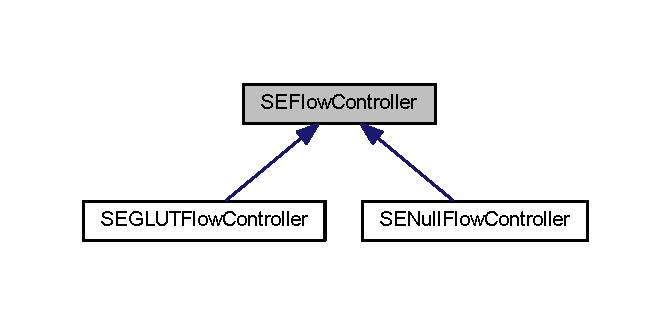
\includegraphics[width=322pt]{class_s_e_flow_controller__inherit__graph}
\end{center}
\end{figure}
\subsection*{Public Types}
\begin{DoxyCompactItemize}
\item 
enum {\bf t\+Flow\+Controller} \{ {\bf N\+U\+L\+L\+\_\+\+F\+C}, 
{\bf G\+L\+U\+T\+\_\+\+F\+C}, 
{\bf N\+U\+M\+\_\+\+F\+C}
 \}
\end{DoxyCompactItemize}
\subsection*{Public Member Functions}
\begin{DoxyCompactItemize}
\item 
virtual void {\bf main\+Loop} ()=0
\item 
virtual void {\bf bind\+Callbacks} ()=0
\item 
{\bf t\+Flow\+Controller} {\bf get\+Type} ()
\item 
void {\bf request\+Exit} ()
\end{DoxyCompactItemize}
\subsection*{Protected Member Functions}
\begin{DoxyCompactItemize}
\item 
{\bf S\+E\+Flow\+Controller} ({\bf t\+Flow\+Controller} t)
\item 
virtual {\bf $\sim$\+S\+E\+Flow\+Controller} ()
\item 
bool {\bf exit\+Requested} ()
\end{DoxyCompactItemize}
\subsection*{Friends}
\begin{DoxyCompactItemize}
\item 
class {\bf S\+E\+Service\+Locator}
\end{DoxyCompactItemize}


\subsection{Detailed Description}


Definition at line 6 of file S\+E\+Flow\+Controller.\+h.



\subsection{Member Enumeration Documentation}
\index{S\+E\+Flow\+Controller@{S\+E\+Flow\+Controller}!t\+Flow\+Controller@{t\+Flow\+Controller}}
\index{t\+Flow\+Controller@{t\+Flow\+Controller}!S\+E\+Flow\+Controller@{S\+E\+Flow\+Controller}}
\subsubsection[{t\+Flow\+Controller}]{\setlength{\rightskip}{0pt plus 5cm}enum {\bf S\+E\+Flow\+Controller\+::t\+Flow\+Controller}}\label{class_s_e_flow_controller_a2ca9e81fa8dc412a8839ebf6aff4c5af}
\begin{Desc}
\item[Enumerator]\par
\begin{description}
\index{N\+U\+L\+L\+\_\+\+F\+C@{N\+U\+L\+L\+\_\+\+F\+C}!S\+E\+Flow\+Controller@{S\+E\+Flow\+Controller}}\index{S\+E\+Flow\+Controller@{S\+E\+Flow\+Controller}!N\+U\+L\+L\+\_\+\+F\+C@{N\+U\+L\+L\+\_\+\+F\+C}}\item[{\em 
N\+U\+L\+L\+\_\+\+F\+C\label{class_s_e_flow_controller_a2ca9e81fa8dc412a8839ebf6aff4c5afa0db9cbc43127ea9b71efa55cb84560e5}
}]\index{G\+L\+U\+T\+\_\+\+F\+C@{G\+L\+U\+T\+\_\+\+F\+C}!S\+E\+Flow\+Controller@{S\+E\+Flow\+Controller}}\index{S\+E\+Flow\+Controller@{S\+E\+Flow\+Controller}!G\+L\+U\+T\+\_\+\+F\+C@{G\+L\+U\+T\+\_\+\+F\+C}}\item[{\em 
G\+L\+U\+T\+\_\+\+F\+C\label{class_s_e_flow_controller_a2ca9e81fa8dc412a8839ebf6aff4c5afa36736697a115f9d76b2ca9f8ca6f9959}
}]\index{N\+U\+M\+\_\+\+F\+C@{N\+U\+M\+\_\+\+F\+C}!S\+E\+Flow\+Controller@{S\+E\+Flow\+Controller}}\index{S\+E\+Flow\+Controller@{S\+E\+Flow\+Controller}!N\+U\+M\+\_\+\+F\+C@{N\+U\+M\+\_\+\+F\+C}}\item[{\em 
N\+U\+M\+\_\+\+F\+C\label{class_s_e_flow_controller_a2ca9e81fa8dc412a8839ebf6aff4c5afad1e2c98decaffe2ff4b94e6b8a87168e}
}]\end{description}
\end{Desc}


Definition at line 11 of file S\+E\+Flow\+Controller.\+h.



\subsection{Constructor \& Destructor Documentation}
\index{S\+E\+Flow\+Controller@{S\+E\+Flow\+Controller}!S\+E\+Flow\+Controller@{S\+E\+Flow\+Controller}}
\index{S\+E\+Flow\+Controller@{S\+E\+Flow\+Controller}!S\+E\+Flow\+Controller@{S\+E\+Flow\+Controller}}
\subsubsection[{S\+E\+Flow\+Controller}]{\setlength{\rightskip}{0pt plus 5cm}S\+E\+Flow\+Controller\+::\+S\+E\+Flow\+Controller (
\begin{DoxyParamCaption}
\item[{{\bf t\+Flow\+Controller}}]{t}
\end{DoxyParamCaption}
)\hspace{0.3cm}{\ttfamily [inline]}, {\ttfamily [protected]}}\label{class_s_e_flow_controller_aeb9887dc9b0371e34bf41701f06c9092}


Definition at line 21 of file S\+E\+Flow\+Controller.\+h.

\index{S\+E\+Flow\+Controller@{S\+E\+Flow\+Controller}!````~S\+E\+Flow\+Controller@{$\sim$\+S\+E\+Flow\+Controller}}
\index{````~S\+E\+Flow\+Controller@{$\sim$\+S\+E\+Flow\+Controller}!S\+E\+Flow\+Controller@{S\+E\+Flow\+Controller}}
\subsubsection[{$\sim$\+S\+E\+Flow\+Controller}]{\setlength{\rightskip}{0pt plus 5cm}virtual S\+E\+Flow\+Controller\+::$\sim$\+S\+E\+Flow\+Controller (
\begin{DoxyParamCaption}
{}
\end{DoxyParamCaption}
)\hspace{0.3cm}{\ttfamily [inline]}, {\ttfamily [protected]}, {\ttfamily [virtual]}}\label{class_s_e_flow_controller_a923e0a2a9a72ec765b132130bae89b37}


Definition at line 22 of file S\+E\+Flow\+Controller.\+h.



\subsection{Member Function Documentation}
\index{S\+E\+Flow\+Controller@{S\+E\+Flow\+Controller}!bind\+Callbacks@{bind\+Callbacks}}
\index{bind\+Callbacks@{bind\+Callbacks}!S\+E\+Flow\+Controller@{S\+E\+Flow\+Controller}}
\subsubsection[{bind\+Callbacks}]{\setlength{\rightskip}{0pt plus 5cm}virtual void S\+E\+Flow\+Controller\+::bind\+Callbacks (
\begin{DoxyParamCaption}
{}
\end{DoxyParamCaption}
)\hspace{0.3cm}{\ttfamily [pure virtual]}}\label{class_s_e_flow_controller_a7ce1c8c45745d5626398598662a6e72e}


Implemented in {\bf S\+E\+Null\+Flow\+Controller} \doxyref{}{p.}{class_s_e_null_flow_controller_a67232e62806d2b576f521516341b2327}, and {\bf S\+E\+G\+L\+U\+T\+Flow\+Controller} \doxyref{}{p.}{class_s_e_g_l_u_t_flow_controller_a3107f0bfa1e911ba020fa93ae8e940f7}.

\index{S\+E\+Flow\+Controller@{S\+E\+Flow\+Controller}!exit\+Requested@{exit\+Requested}}
\index{exit\+Requested@{exit\+Requested}!S\+E\+Flow\+Controller@{S\+E\+Flow\+Controller}}
\subsubsection[{exit\+Requested}]{\setlength{\rightskip}{0pt plus 5cm}bool S\+E\+Flow\+Controller\+::exit\+Requested (
\begin{DoxyParamCaption}
{}
\end{DoxyParamCaption}
)\hspace{0.3cm}{\ttfamily [inline]}, {\ttfamily [protected]}}\label{class_s_e_flow_controller_adcf88c3ae71c790d546fca930293a801}


Definition at line 24 of file S\+E\+Flow\+Controller.\+h.

\index{S\+E\+Flow\+Controller@{S\+E\+Flow\+Controller}!get\+Type@{get\+Type}}
\index{get\+Type@{get\+Type}!S\+E\+Flow\+Controller@{S\+E\+Flow\+Controller}}
\subsubsection[{get\+Type}]{\setlength{\rightskip}{0pt plus 5cm}{\bf t\+Flow\+Controller} S\+E\+Flow\+Controller\+::get\+Type (
\begin{DoxyParamCaption}
{}
\end{DoxyParamCaption}
)\hspace{0.3cm}{\ttfamily [inline]}}\label{class_s_e_flow_controller_a7707eeb043bf25947f24c6c7ab811997}


Definition at line 16 of file S\+E\+Flow\+Controller.\+h.

\index{S\+E\+Flow\+Controller@{S\+E\+Flow\+Controller}!main\+Loop@{main\+Loop}}
\index{main\+Loop@{main\+Loop}!S\+E\+Flow\+Controller@{S\+E\+Flow\+Controller}}
\subsubsection[{main\+Loop}]{\setlength{\rightskip}{0pt plus 5cm}virtual void S\+E\+Flow\+Controller\+::main\+Loop (
\begin{DoxyParamCaption}
{}
\end{DoxyParamCaption}
)\hspace{0.3cm}{\ttfamily [pure virtual]}}\label{class_s_e_flow_controller_a66f3714c1697c7b040e6c6f09374953b}


Implemented in {\bf S\+E\+Null\+Flow\+Controller} \doxyref{}{p.}{class_s_e_null_flow_controller_a9498c332f22bec64c769592948d2eb3b}, and {\bf S\+E\+G\+L\+U\+T\+Flow\+Controller} \doxyref{}{p.}{class_s_e_g_l_u_t_flow_controller_ad580e608fafbc0a48d30985e8bc9f7f2}.

\index{S\+E\+Flow\+Controller@{S\+E\+Flow\+Controller}!request\+Exit@{request\+Exit}}
\index{request\+Exit@{request\+Exit}!S\+E\+Flow\+Controller@{S\+E\+Flow\+Controller}}
\subsubsection[{request\+Exit}]{\setlength{\rightskip}{0pt plus 5cm}void S\+E\+Flow\+Controller\+::request\+Exit (
\begin{DoxyParamCaption}
{}
\end{DoxyParamCaption}
)\hspace{0.3cm}{\ttfamily [inline]}}\label{class_s_e_flow_controller_a544d65bf412307b71fced345881eb968}


Definition at line 18 of file S\+E\+Flow\+Controller.\+h.



\subsection{Friends And Related Function Documentation}
\index{S\+E\+Flow\+Controller@{S\+E\+Flow\+Controller}!S\+E\+Service\+Locator@{S\+E\+Service\+Locator}}
\index{S\+E\+Service\+Locator@{S\+E\+Service\+Locator}!S\+E\+Flow\+Controller@{S\+E\+Flow\+Controller}}
\subsubsection[{S\+E\+Service\+Locator}]{\setlength{\rightskip}{0pt plus 5cm}friend class {\bf S\+E\+Service\+Locator}\hspace{0.3cm}{\ttfamily [friend]}}\label{class_s_e_flow_controller_ab6e41e6b8528b0fe19953837048fbde6}


Definition at line 8 of file S\+E\+Flow\+Controller.\+h.



The documentation for this class was generated from the following file\+:\begin{DoxyCompactItemize}
\item 
{\bf S\+E\+Flow\+Controller.\+h}\end{DoxyCompactItemize}

\section{S\+E\+Frustum\+Type Struct Reference}
\label{struct_s_e_frustum_type}\index{S\+E\+Frustum\+Type@{S\+E\+Frustum\+Type}}


{\ttfamily \#include $<$S\+E\+Camera.\+h$>$}

\subsection*{Public Types}
\begin{DoxyCompactItemize}
\item 
enum {\bf t\+Frustum} \{ {\bf O\+R\+T\+H\+O}, 
{\bf P\+E\+R\+S\+P\+E\+C\+T\+I\+V\+E}
 \}
\end{DoxyCompactItemize}


\subsection{Detailed Description}


Definition at line 13 of file S\+E\+Camera.\+h.



\subsection{Member Enumeration Documentation}
\index{S\+E\+Frustum\+Type@{S\+E\+Frustum\+Type}!t\+Frustum@{t\+Frustum}}
\index{t\+Frustum@{t\+Frustum}!S\+E\+Frustum\+Type@{S\+E\+Frustum\+Type}}
\subsubsection[{t\+Frustum}]{\setlength{\rightskip}{0pt plus 5cm}enum {\bf S\+E\+Frustum\+Type\+::t\+Frustum}}\label{struct_s_e_frustum_type_a990ede233f2b127b44dd80bf651a958c}
\begin{Desc}
\item[Enumerator]\par
\begin{description}
\index{O\+R\+T\+H\+O@{O\+R\+T\+H\+O}!S\+E\+Frustum\+Type@{S\+E\+Frustum\+Type}}\index{S\+E\+Frustum\+Type@{S\+E\+Frustum\+Type}!O\+R\+T\+H\+O@{O\+R\+T\+H\+O}}\item[{\em 
O\+R\+T\+H\+O\label{struct_s_e_frustum_type_a990ede233f2b127b44dd80bf651a958cae8c90da5cee48ec7195171e787189189}
}]\index{P\+E\+R\+S\+P\+E\+C\+T\+I\+V\+E@{P\+E\+R\+S\+P\+E\+C\+T\+I\+V\+E}!S\+E\+Frustum\+Type@{S\+E\+Frustum\+Type}}\index{S\+E\+Frustum\+Type@{S\+E\+Frustum\+Type}!P\+E\+R\+S\+P\+E\+C\+T\+I\+V\+E@{P\+E\+R\+S\+P\+E\+C\+T\+I\+V\+E}}\item[{\em 
P\+E\+R\+S\+P\+E\+C\+T\+I\+V\+E\label{struct_s_e_frustum_type_a990ede233f2b127b44dd80bf651a958cae3f3ace861ef652b78b34ab664b440a3}
}]\end{description}
\end{Desc}


Definition at line 15 of file S\+E\+Camera.\+h.



The documentation for this struct was generated from the following file\+:\begin{DoxyCompactItemize}
\item 
{\bf S\+E\+Camera.\+h}\end{DoxyCompactItemize}

\section{S\+E\+G\+L\+U\+I\+Window Class Reference}
\label{class_s_e_g_l_u_i_window}\index{S\+E\+G\+L\+U\+I\+Window@{S\+E\+G\+L\+U\+I\+Window}}


{\ttfamily \#include $<$S\+E\+G\+L\+U\+I\+Window.\+h$>$}



Inheritance diagram for S\+E\+G\+L\+U\+I\+Window\+:
\nopagebreak
\begin{figure}[H]
\begin{center}
\leavevmode
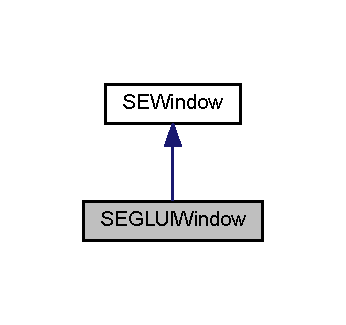
\includegraphics[width=166pt]{class_s_e_g_l_u_i_window__inherit__graph}
\end{center}
\end{figure}


Collaboration diagram for S\+E\+G\+L\+U\+I\+Window\+:
\nopagebreak
\begin{figure}[H]
\begin{center}
\leavevmode
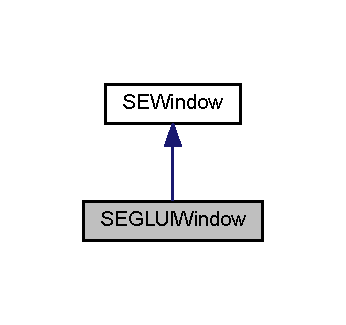
\includegraphics[width=166pt]{class_s_e_g_l_u_i_window__coll__graph}
\end{center}
\end{figure}
\subsection*{Public Member Functions}
\begin{DoxyCompactItemize}
\item 
virtual void {\bf reshape} (int nw, int nh)
\item 
virtual void {\bf redisplay} ()
\end{DoxyCompactItemize}
\subsection*{Protected Member Functions}
\begin{DoxyCompactItemize}
\item 
{\bf S\+E\+G\+L\+U\+I\+Window} (int w, int h, std\+::string t=\char`\"{}\char`\"{}, int px=0, int py=0)
\item 
virtual {\bf $\sim$\+S\+E\+G\+L\+U\+I\+Window} ()
\end{DoxyCompactItemize}
\subsection*{Friends}
\begin{DoxyCompactItemize}
\item 
class {\bf S\+E\+G\+L\+U\+I\+Window\+Manager}
\end{DoxyCompactItemize}
\subsection*{Additional Inherited Members}


\subsection{Detailed Description}


Definition at line 11 of file S\+E\+G\+L\+U\+I\+Window.\+h.



\subsection{Constructor \& Destructor Documentation}
\index{S\+E\+G\+L\+U\+I\+Window@{S\+E\+G\+L\+U\+I\+Window}!S\+E\+G\+L\+U\+I\+Window@{S\+E\+G\+L\+U\+I\+Window}}
\index{S\+E\+G\+L\+U\+I\+Window@{S\+E\+G\+L\+U\+I\+Window}!S\+E\+G\+L\+U\+I\+Window@{S\+E\+G\+L\+U\+I\+Window}}
\subsubsection[{S\+E\+G\+L\+U\+I\+Window}]{\setlength{\rightskip}{0pt plus 5cm}S\+E\+G\+L\+U\+I\+Window\+::\+S\+E\+G\+L\+U\+I\+Window (
\begin{DoxyParamCaption}
\item[{int}]{w, }
\item[{int}]{h, }
\item[{std\+::string}]{t = {\ttfamily \char`\"{}\char`\"{}}, }
\item[{int}]{px = {\ttfamily 0}, }
\item[{int}]{py = {\ttfamily 0}}
\end{DoxyParamCaption}
)\hspace{0.3cm}{\ttfamily [protected]}}\label{class_s_e_g_l_u_i_window_ad5ff3d62a224a15e1beb04ac188de25f}


Definition at line 5 of file S\+E\+G\+L\+U\+I\+Window.\+cpp.

\index{S\+E\+G\+L\+U\+I\+Window@{S\+E\+G\+L\+U\+I\+Window}!````~S\+E\+G\+L\+U\+I\+Window@{$\sim$\+S\+E\+G\+L\+U\+I\+Window}}
\index{````~S\+E\+G\+L\+U\+I\+Window@{$\sim$\+S\+E\+G\+L\+U\+I\+Window}!S\+E\+G\+L\+U\+I\+Window@{S\+E\+G\+L\+U\+I\+Window}}
\subsubsection[{$\sim$\+S\+E\+G\+L\+U\+I\+Window}]{\setlength{\rightskip}{0pt plus 5cm}S\+E\+G\+L\+U\+I\+Window\+::$\sim$\+S\+E\+G\+L\+U\+I\+Window (
\begin{DoxyParamCaption}
{}
\end{DoxyParamCaption}
)\hspace{0.3cm}{\ttfamily [protected]}, {\ttfamily [virtual]}}\label{class_s_e_g_l_u_i_window_ade47113ce0bfff0b6714e1cf43e8d0bc}


Definition at line 16 of file S\+E\+G\+L\+U\+I\+Window.\+cpp.



\subsection{Member Function Documentation}
\index{S\+E\+G\+L\+U\+I\+Window@{S\+E\+G\+L\+U\+I\+Window}!redisplay@{redisplay}}
\index{redisplay@{redisplay}!S\+E\+G\+L\+U\+I\+Window@{S\+E\+G\+L\+U\+I\+Window}}
\subsubsection[{redisplay}]{\setlength{\rightskip}{0pt plus 5cm}void S\+E\+G\+L\+U\+I\+Window\+::redisplay (
\begin{DoxyParamCaption}
{}
\end{DoxyParamCaption}
)\hspace{0.3cm}{\ttfamily [virtual]}}\label{class_s_e_g_l_u_i_window_a174f43c7e6019ec10119ef821401f592}


Reimplemented from {\bf S\+E\+Window} \doxyref{}{p.}{class_s_e_window_a3364bf6038ddf6c815b5bed2fafcb2c8}.



Definition at line 34 of file S\+E\+G\+L\+U\+I\+Window.\+cpp.

\index{S\+E\+G\+L\+U\+I\+Window@{S\+E\+G\+L\+U\+I\+Window}!reshape@{reshape}}
\index{reshape@{reshape}!S\+E\+G\+L\+U\+I\+Window@{S\+E\+G\+L\+U\+I\+Window}}
\subsubsection[{reshape}]{\setlength{\rightskip}{0pt plus 5cm}void S\+E\+G\+L\+U\+I\+Window\+::reshape (
\begin{DoxyParamCaption}
\item[{int}]{nw, }
\item[{int}]{nh}
\end{DoxyParamCaption}
)\hspace{0.3cm}{\ttfamily [virtual]}}\label{class_s_e_g_l_u_i_window_a46bf43faff641d771f2507df91e76f14}


Reimplemented from {\bf S\+E\+Window} \doxyref{}{p.}{class_s_e_window_a9cb36f97a0a759d9aa3a2c1978f0ccdc}.



Definition at line 28 of file S\+E\+G\+L\+U\+I\+Window.\+cpp.



Here is the call graph for this function\+:
\nopagebreak
\begin{figure}[H]
\begin{center}
\leavevmode
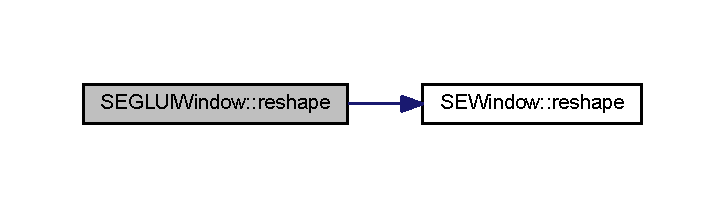
\includegraphics[width=348pt]{class_s_e_g_l_u_i_window_a46bf43faff641d771f2507df91e76f14_cgraph}
\end{center}
\end{figure}




\subsection{Friends And Related Function Documentation}
\index{S\+E\+G\+L\+U\+I\+Window@{S\+E\+G\+L\+U\+I\+Window}!S\+E\+G\+L\+U\+I\+Window\+Manager@{S\+E\+G\+L\+U\+I\+Window\+Manager}}
\index{S\+E\+G\+L\+U\+I\+Window\+Manager@{S\+E\+G\+L\+U\+I\+Window\+Manager}!S\+E\+G\+L\+U\+I\+Window@{S\+E\+G\+L\+U\+I\+Window}}
\subsubsection[{S\+E\+G\+L\+U\+I\+Window\+Manager}]{\setlength{\rightskip}{0pt plus 5cm}friend class {\bf S\+E\+G\+L\+U\+I\+Window\+Manager}\hspace{0.3cm}{\ttfamily [friend]}}\label{class_s_e_g_l_u_i_window_a7d38f09596b815dd13a24f8edd4f015d}


Definition at line 13 of file S\+E\+G\+L\+U\+I\+Window.\+h.



The documentation for this class was generated from the following files\+:\begin{DoxyCompactItemize}
\item 
{\bf S\+E\+G\+L\+U\+I\+Window.\+h}\item 
{\bf S\+E\+G\+L\+U\+I\+Window.\+cpp}\end{DoxyCompactItemize}

\section{S\+E\+G\+L\+U\+I\+Window\+Manager Class Reference}
\label{class_s_e_g_l_u_i_window_manager}\index{S\+E\+G\+L\+U\+I\+Window\+Manager@{S\+E\+G\+L\+U\+I\+Window\+Manager}}


{\ttfamily \#include $<$S\+E\+G\+L\+U\+I\+Window\+Manager.\+h$>$}



Inheritance diagram for S\+E\+G\+L\+U\+I\+Window\+Manager\+:
\nopagebreak
\begin{figure}[H]
\begin{center}
\leavevmode
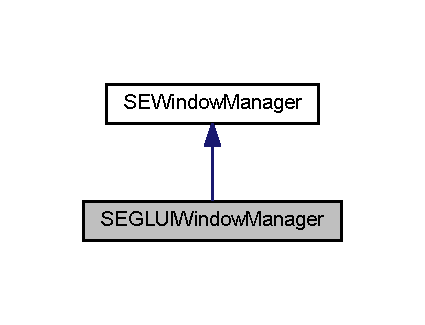
\includegraphics[width=204pt]{class_s_e_g_l_u_i_window_manager__inherit__graph}
\end{center}
\end{figure}


Collaboration diagram for S\+E\+G\+L\+U\+I\+Window\+Manager\+:
\nopagebreak
\begin{figure}[H]
\begin{center}
\leavevmode
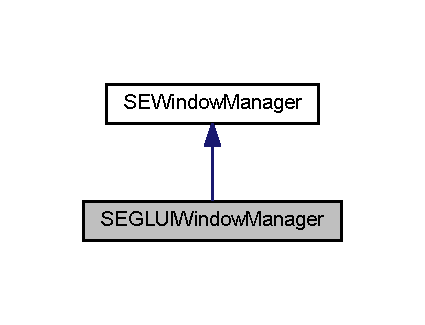
\includegraphics[width=204pt]{class_s_e_g_l_u_i_window_manager__coll__graph}
\end{center}
\end{figure}
\subsection*{Public Member Functions}
\begin{DoxyCompactItemize}
\item 
virtual long {\bf create\+New\+Window} (int w, int h, std\+::string t=\char`\"{}\char`\"{}, int posx=0, int posy=0)
\item 
virtual void {\bf register\+Display\+Function} (void($\ast$f)(void))
\item 
virtual void {\bf register\+Reshape\+Function} (void($\ast$f)(int, int))
\item 
virtual void {\bf register\+Idle\+Function} (void($\ast$f)(void))
\end{DoxyCompactItemize}
\subsection*{Protected Member Functions}
\begin{DoxyCompactItemize}
\item 
{\bf S\+E\+G\+L\+U\+I\+Window\+Manager} ()
\item 
{\bf S\+E\+G\+L\+U\+I\+Window\+Manager} (int argc, char $\ast$$\ast$argv)
\item 
virtual {\bf $\sim$\+S\+E\+G\+L\+U\+I\+Window\+Manager} ()
\end{DoxyCompactItemize}
\subsection*{Friends}
\begin{DoxyCompactItemize}
\item 
class {\bf S\+E\+Service\+Locator}
\end{DoxyCompactItemize}
\subsection*{Additional Inherited Members}


\subsection{Detailed Description}


Definition at line 9 of file S\+E\+G\+L\+U\+I\+Window\+Manager.\+h.



\subsection{Constructor \& Destructor Documentation}
\index{S\+E\+G\+L\+U\+I\+Window\+Manager@{S\+E\+G\+L\+U\+I\+Window\+Manager}!S\+E\+G\+L\+U\+I\+Window\+Manager@{S\+E\+G\+L\+U\+I\+Window\+Manager}}
\index{S\+E\+G\+L\+U\+I\+Window\+Manager@{S\+E\+G\+L\+U\+I\+Window\+Manager}!S\+E\+G\+L\+U\+I\+Window\+Manager@{S\+E\+G\+L\+U\+I\+Window\+Manager}}
\subsubsection[{S\+E\+G\+L\+U\+I\+Window\+Manager}]{\setlength{\rightskip}{0pt plus 5cm}S\+E\+G\+L\+U\+I\+Window\+Manager\+::\+S\+E\+G\+L\+U\+I\+Window\+Manager (
\begin{DoxyParamCaption}
{}
\end{DoxyParamCaption}
)\hspace{0.3cm}{\ttfamily [protected]}}\label{class_s_e_g_l_u_i_window_manager_a4ed3cb6ddf97c87edd0456cc3e6f2288}


Definition at line 4 of file S\+E\+G\+L\+U\+I\+Window\+Manager.\+cpp.

\index{S\+E\+G\+L\+U\+I\+Window\+Manager@{S\+E\+G\+L\+U\+I\+Window\+Manager}!S\+E\+G\+L\+U\+I\+Window\+Manager@{S\+E\+G\+L\+U\+I\+Window\+Manager}}
\index{S\+E\+G\+L\+U\+I\+Window\+Manager@{S\+E\+G\+L\+U\+I\+Window\+Manager}!S\+E\+G\+L\+U\+I\+Window\+Manager@{S\+E\+G\+L\+U\+I\+Window\+Manager}}
\subsubsection[{S\+E\+G\+L\+U\+I\+Window\+Manager}]{\setlength{\rightskip}{0pt plus 5cm}S\+E\+G\+L\+U\+I\+Window\+Manager\+::\+S\+E\+G\+L\+U\+I\+Window\+Manager (
\begin{DoxyParamCaption}
\item[{int}]{argc, }
\item[{char $\ast$$\ast$}]{argv}
\end{DoxyParamCaption}
)\hspace{0.3cm}{\ttfamily [protected]}}\label{class_s_e_g_l_u_i_window_manager_a7ddeae289dd02fb073df3a441921ba56}


Definition at line 9 of file S\+E\+G\+L\+U\+I\+Window\+Manager.\+cpp.

\index{S\+E\+G\+L\+U\+I\+Window\+Manager@{S\+E\+G\+L\+U\+I\+Window\+Manager}!````~S\+E\+G\+L\+U\+I\+Window\+Manager@{$\sim$\+S\+E\+G\+L\+U\+I\+Window\+Manager}}
\index{````~S\+E\+G\+L\+U\+I\+Window\+Manager@{$\sim$\+S\+E\+G\+L\+U\+I\+Window\+Manager}!S\+E\+G\+L\+U\+I\+Window\+Manager@{S\+E\+G\+L\+U\+I\+Window\+Manager}}
\subsubsection[{$\sim$\+S\+E\+G\+L\+U\+I\+Window\+Manager}]{\setlength{\rightskip}{0pt plus 5cm}virtual S\+E\+G\+L\+U\+I\+Window\+Manager\+::$\sim$\+S\+E\+G\+L\+U\+I\+Window\+Manager (
\begin{DoxyParamCaption}
{}
\end{DoxyParamCaption}
)\hspace{0.3cm}{\ttfamily [inline]}, {\ttfamily [protected]}, {\ttfamily [virtual]}}\label{class_s_e_g_l_u_i_window_manager_a310f3c992bc7015d54111e01aeef34c3}


Definition at line 16 of file S\+E\+G\+L\+U\+I\+Window\+Manager.\+h.



\subsection{Member Function Documentation}
\index{S\+E\+G\+L\+U\+I\+Window\+Manager@{S\+E\+G\+L\+U\+I\+Window\+Manager}!create\+New\+Window@{create\+New\+Window}}
\index{create\+New\+Window@{create\+New\+Window}!S\+E\+G\+L\+U\+I\+Window\+Manager@{S\+E\+G\+L\+U\+I\+Window\+Manager}}
\subsubsection[{create\+New\+Window}]{\setlength{\rightskip}{0pt plus 5cm}long S\+E\+G\+L\+U\+I\+Window\+Manager\+::create\+New\+Window (
\begin{DoxyParamCaption}
\item[{int}]{w, }
\item[{int}]{h, }
\item[{std\+::string}]{t = {\ttfamily \char`\"{}\char`\"{}}, }
\item[{int}]{posx = {\ttfamily 0}, }
\item[{int}]{posy = {\ttfamily 0}}
\end{DoxyParamCaption}
)\hspace{0.3cm}{\ttfamily [virtual]}}\label{class_s_e_g_l_u_i_window_manager_afd551aecb6a9b737add9d1a2900bee6d}


Implements {\bf S\+E\+Window\+Manager} \doxyref{}{p.}{class_s_e_window_manager_abfa1eaa96f122ad1715932226986dfdd}.



Definition at line 15 of file S\+E\+G\+L\+U\+I\+Window\+Manager.\+cpp.



Here is the call graph for this function\+:
\nopagebreak
\begin{figure}[H]
\begin{center}
\leavevmode
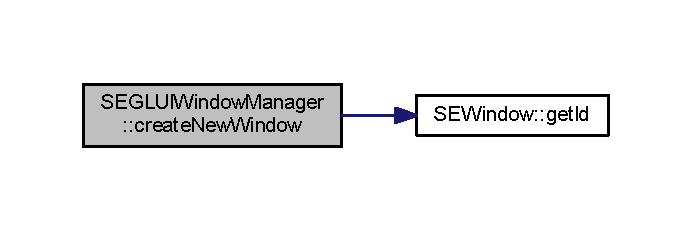
\includegraphics[width=332pt]{class_s_e_g_l_u_i_window_manager_afd551aecb6a9b737add9d1a2900bee6d_cgraph}
\end{center}
\end{figure}


\index{S\+E\+G\+L\+U\+I\+Window\+Manager@{S\+E\+G\+L\+U\+I\+Window\+Manager}!register\+Display\+Function@{register\+Display\+Function}}
\index{register\+Display\+Function@{register\+Display\+Function}!S\+E\+G\+L\+U\+I\+Window\+Manager@{S\+E\+G\+L\+U\+I\+Window\+Manager}}
\subsubsection[{register\+Display\+Function}]{\setlength{\rightskip}{0pt plus 5cm}void S\+E\+G\+L\+U\+I\+Window\+Manager\+::register\+Display\+Function (
\begin{DoxyParamCaption}
\item[{void($\ast$)(void)}]{f}
\end{DoxyParamCaption}
)\hspace{0.3cm}{\ttfamily [virtual]}}\label{class_s_e_g_l_u_i_window_manager_a9ccd055b39f6f87c210870d6ba3ac0e5}


Implements {\bf S\+E\+Window\+Manager} \doxyref{}{p.}{class_s_e_window_manager_aa86172a5046bfb5d02d59405bdfef595}.



Definition at line 24 of file S\+E\+G\+L\+U\+I\+Window\+Manager.\+cpp.

\index{S\+E\+G\+L\+U\+I\+Window\+Manager@{S\+E\+G\+L\+U\+I\+Window\+Manager}!register\+Idle\+Function@{register\+Idle\+Function}}
\index{register\+Idle\+Function@{register\+Idle\+Function}!S\+E\+G\+L\+U\+I\+Window\+Manager@{S\+E\+G\+L\+U\+I\+Window\+Manager}}
\subsubsection[{register\+Idle\+Function}]{\setlength{\rightskip}{0pt plus 5cm}void S\+E\+G\+L\+U\+I\+Window\+Manager\+::register\+Idle\+Function (
\begin{DoxyParamCaption}
\item[{void($\ast$)(void)}]{f}
\end{DoxyParamCaption}
)\hspace{0.3cm}{\ttfamily [virtual]}}\label{class_s_e_g_l_u_i_window_manager_a66bd4ecdbeb466935f2f7127c31a45b8}


Implements {\bf S\+E\+Window\+Manager} \doxyref{}{p.}{class_s_e_window_manager_af728b393a7f2f55da92aa4e963d00678}.



Definition at line 34 of file S\+E\+G\+L\+U\+I\+Window\+Manager.\+cpp.

\index{S\+E\+G\+L\+U\+I\+Window\+Manager@{S\+E\+G\+L\+U\+I\+Window\+Manager}!register\+Reshape\+Function@{register\+Reshape\+Function}}
\index{register\+Reshape\+Function@{register\+Reshape\+Function}!S\+E\+G\+L\+U\+I\+Window\+Manager@{S\+E\+G\+L\+U\+I\+Window\+Manager}}
\subsubsection[{register\+Reshape\+Function}]{\setlength{\rightskip}{0pt plus 5cm}void S\+E\+G\+L\+U\+I\+Window\+Manager\+::register\+Reshape\+Function (
\begin{DoxyParamCaption}
\item[{void($\ast$)(int, int)}]{f}
\end{DoxyParamCaption}
)\hspace{0.3cm}{\ttfamily [virtual]}}\label{class_s_e_g_l_u_i_window_manager_a926dd9698ca4f20d8e38e389405aab3a}


Implements {\bf S\+E\+Window\+Manager} \doxyref{}{p.}{class_s_e_window_manager_a5dbd6ff65c50beab87bede6b14e0faef}.



Definition at line 29 of file S\+E\+G\+L\+U\+I\+Window\+Manager.\+cpp.



\subsection{Friends And Related Function Documentation}
\index{S\+E\+G\+L\+U\+I\+Window\+Manager@{S\+E\+G\+L\+U\+I\+Window\+Manager}!S\+E\+Service\+Locator@{S\+E\+Service\+Locator}}
\index{S\+E\+Service\+Locator@{S\+E\+Service\+Locator}!S\+E\+G\+L\+U\+I\+Window\+Manager@{S\+E\+G\+L\+U\+I\+Window\+Manager}}
\subsubsection[{S\+E\+Service\+Locator}]{\setlength{\rightskip}{0pt plus 5cm}friend class {\bf S\+E\+Service\+Locator}\hspace{0.3cm}{\ttfamily [friend]}}\label{class_s_e_g_l_u_i_window_manager_ab6e41e6b8528b0fe19953837048fbde6}


Definition at line 11 of file S\+E\+G\+L\+U\+I\+Window\+Manager.\+h.



The documentation for this class was generated from the following files\+:\begin{DoxyCompactItemize}
\item 
{\bf S\+E\+G\+L\+U\+I\+Window\+Manager.\+h}\item 
{\bf S\+E\+G\+L\+U\+I\+Window\+Manager.\+cpp}\end{DoxyCompactItemize}

\section{S\+E\+G\+L\+U\+T\+Flow\+Controller Class Reference}
\label{class_s_e_g_l_u_t_flow_controller}\index{S\+E\+G\+L\+U\+T\+Flow\+Controller@{S\+E\+G\+L\+U\+T\+Flow\+Controller}}


{\ttfamily \#include $<$S\+E\+G\+L\+U\+T\+Flow\+Controller.\+h$>$}



Inheritance diagram for S\+E\+G\+L\+U\+T\+Flow\+Controller\+:
\nopagebreak
\begin{figure}[H]
\begin{center}
\leavevmode
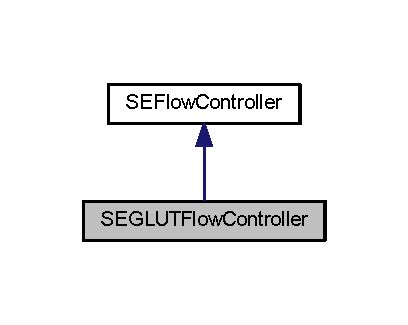
\includegraphics[width=196pt]{class_s_e_g_l_u_t_flow_controller__inherit__graph}
\end{center}
\end{figure}


Collaboration diagram for S\+E\+G\+L\+U\+T\+Flow\+Controller\+:
\nopagebreak
\begin{figure}[H]
\begin{center}
\leavevmode
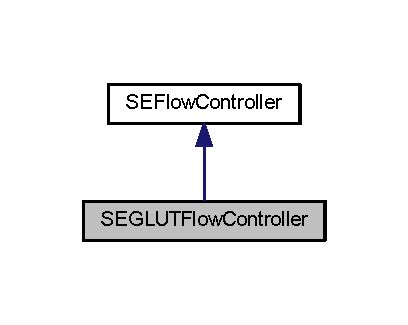
\includegraphics[width=196pt]{class_s_e_g_l_u_t_flow_controller__coll__graph}
\end{center}
\end{figure}
\subsection*{Public Member Functions}
\begin{DoxyCompactItemize}
\item 
{\bf S\+E\+G\+L\+U\+T\+Flow\+Controller} ()
\item 
{\bf $\sim$\+S\+E\+G\+L\+U\+T\+Flow\+Controller} ()
\item 
virtual void {\bf main\+Loop} ()
\item 
virtual void {\bf bind\+Callbacks} ()
\end{DoxyCompactItemize}
\subsection*{Additional Inherited Members}


\subsection{Detailed Description}


Definition at line 9 of file S\+E\+G\+L\+U\+T\+Flow\+Controller.\+h.



\subsection{Constructor \& Destructor Documentation}
\index{S\+E\+G\+L\+U\+T\+Flow\+Controller@{S\+E\+G\+L\+U\+T\+Flow\+Controller}!S\+E\+G\+L\+U\+T\+Flow\+Controller@{S\+E\+G\+L\+U\+T\+Flow\+Controller}}
\index{S\+E\+G\+L\+U\+T\+Flow\+Controller@{S\+E\+G\+L\+U\+T\+Flow\+Controller}!S\+E\+G\+L\+U\+T\+Flow\+Controller@{S\+E\+G\+L\+U\+T\+Flow\+Controller}}
\subsubsection[{S\+E\+G\+L\+U\+T\+Flow\+Controller}]{\setlength{\rightskip}{0pt plus 5cm}S\+E\+G\+L\+U\+T\+Flow\+Controller\+::\+S\+E\+G\+L\+U\+T\+Flow\+Controller (
\begin{DoxyParamCaption}
{}
\end{DoxyParamCaption}
)}\label{class_s_e_g_l_u_t_flow_controller_afe3330a2ce19983be2f8316895337849}


Definition at line 9 of file S\+E\+G\+L\+U\+T\+Flow\+Controller.\+cpp.

\index{S\+E\+G\+L\+U\+T\+Flow\+Controller@{S\+E\+G\+L\+U\+T\+Flow\+Controller}!````~S\+E\+G\+L\+U\+T\+Flow\+Controller@{$\sim$\+S\+E\+G\+L\+U\+T\+Flow\+Controller}}
\index{````~S\+E\+G\+L\+U\+T\+Flow\+Controller@{$\sim$\+S\+E\+G\+L\+U\+T\+Flow\+Controller}!S\+E\+G\+L\+U\+T\+Flow\+Controller@{S\+E\+G\+L\+U\+T\+Flow\+Controller}}
\subsubsection[{$\sim$\+S\+E\+G\+L\+U\+T\+Flow\+Controller}]{\setlength{\rightskip}{0pt plus 5cm}S\+E\+G\+L\+U\+T\+Flow\+Controller\+::$\sim$\+S\+E\+G\+L\+U\+T\+Flow\+Controller (
\begin{DoxyParamCaption}
{}
\end{DoxyParamCaption}
)\hspace{0.3cm}{\ttfamily [inline]}}\label{class_s_e_g_l_u_t_flow_controller_a2ba7fb3270fc4099429e42774113482a}


Definition at line 13 of file S\+E\+G\+L\+U\+T\+Flow\+Controller.\+h.



\subsection{Member Function Documentation}
\index{S\+E\+G\+L\+U\+T\+Flow\+Controller@{S\+E\+G\+L\+U\+T\+Flow\+Controller}!bind\+Callbacks@{bind\+Callbacks}}
\index{bind\+Callbacks@{bind\+Callbacks}!S\+E\+G\+L\+U\+T\+Flow\+Controller@{S\+E\+G\+L\+U\+T\+Flow\+Controller}}
\subsubsection[{bind\+Callbacks}]{\setlength{\rightskip}{0pt plus 5cm}void S\+E\+G\+L\+U\+T\+Flow\+Controller\+::bind\+Callbacks (
\begin{DoxyParamCaption}
{}
\end{DoxyParamCaption}
)\hspace{0.3cm}{\ttfamily [virtual]}}\label{class_s_e_g_l_u_t_flow_controller_a3107f0bfa1e911ba020fa93ae8e940f7}


Implements {\bf S\+E\+Flow\+Controller} \doxyref{}{p.}{class_s_e_flow_controller_a7ce1c8c45745d5626398598662a6e72e}.



Definition at line 15 of file S\+E\+G\+L\+U\+T\+Flow\+Controller.\+cpp.



Here is the call graph for this function\+:
\nopagebreak
\begin{figure}[H]
\begin{center}
\leavevmode
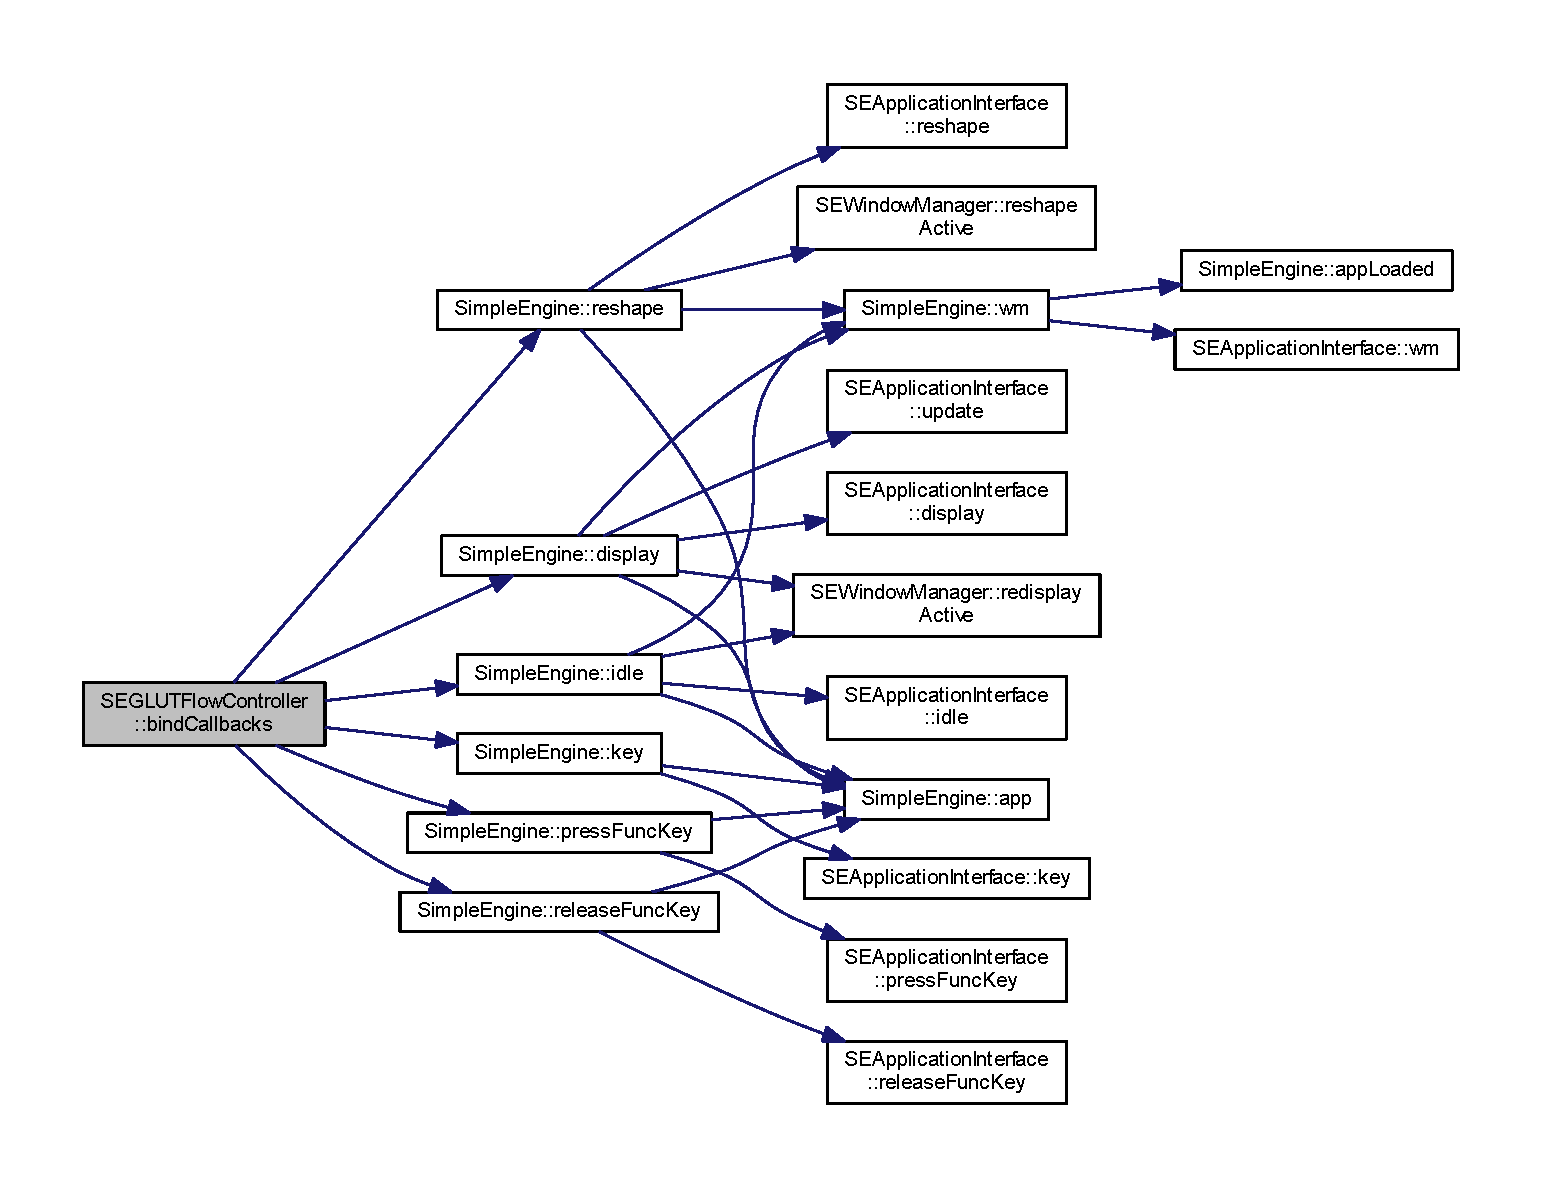
\includegraphics[width=350pt]{class_s_e_g_l_u_t_flow_controller_a3107f0bfa1e911ba020fa93ae8e940f7_cgraph}
\end{center}
\end{figure}


\index{S\+E\+G\+L\+U\+T\+Flow\+Controller@{S\+E\+G\+L\+U\+T\+Flow\+Controller}!main\+Loop@{main\+Loop}}
\index{main\+Loop@{main\+Loop}!S\+E\+G\+L\+U\+T\+Flow\+Controller@{S\+E\+G\+L\+U\+T\+Flow\+Controller}}
\subsubsection[{main\+Loop}]{\setlength{\rightskip}{0pt plus 5cm}void S\+E\+G\+L\+U\+T\+Flow\+Controller\+::main\+Loop (
\begin{DoxyParamCaption}
{}
\end{DoxyParamCaption}
)\hspace{0.3cm}{\ttfamily [virtual]}}\label{class_s_e_g_l_u_t_flow_controller_ad580e608fafbc0a48d30985e8bc9f7f2}


Implements {\bf S\+E\+Flow\+Controller} \doxyref{}{p.}{class_s_e_flow_controller_a66f3714c1697c7b040e6c6f09374953b}.



Definition at line 27 of file S\+E\+G\+L\+U\+T\+Flow\+Controller.\+cpp.



Here is the call graph for this function\+:
\nopagebreak
\begin{figure}[H]
\begin{center}
\leavevmode
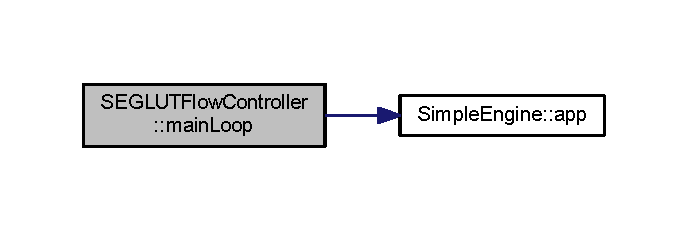
\includegraphics[width=330pt]{class_s_e_g_l_u_t_flow_controller_ad580e608fafbc0a48d30985e8bc9f7f2_cgraph}
\end{center}
\end{figure}




The documentation for this class was generated from the following files\+:\begin{DoxyCompactItemize}
\item 
{\bf S\+E\+G\+L\+U\+T\+Flow\+Controller.\+h}\item 
{\bf S\+E\+G\+L\+U\+T\+Flow\+Controller.\+cpp}\end{DoxyCompactItemize}

\section{S\+E\+Light$<$ T $>$ Class Template Reference}
\label{class_s_e_light}\index{S\+E\+Light$<$ T $>$@{S\+E\+Light$<$ T $>$}}


{\ttfamily \#include $<$S\+E\+Light.\+h$>$}



Inheritance diagram for S\+E\+Light$<$ T $>$\+:
\nopagebreak
\begin{figure}[H]
\begin{center}
\leavevmode
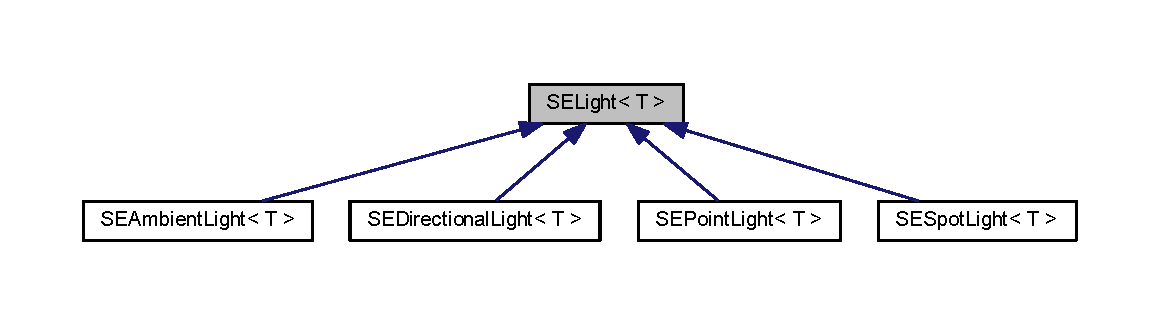
\includegraphics[width=350pt]{class_s_e_light__inherit__graph}
\end{center}
\end{figure}


Collaboration diagram for S\+E\+Light$<$ T $>$\+:
\nopagebreak
\begin{figure}[H]
\begin{center}
\leavevmode
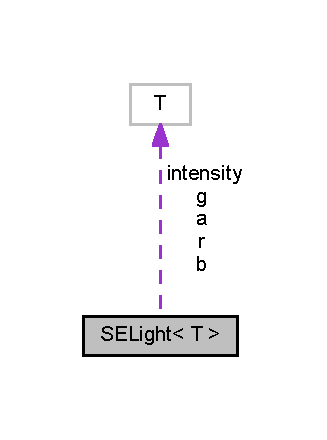
\includegraphics[width=157pt]{class_s_e_light__coll__graph}
\end{center}
\end{figure}
\subsection*{Public Member Functions}
\begin{DoxyCompactItemize}
\item 
virtual {\bf S\+E\+Light}$<$ T $>$ \& {\bf set\+Color} (T {\bf r}, T {\bf g}, T {\bf b}, T {\bf a})
\item 
virtual {\bf S\+E\+Light}$<$ T $>$ \& {\bf set\+Color} (T {\bf r}, T {\bf g}, T {\bf b})
\item 
virtual {\bf S\+E\+Light}$<$ T $>$ \& {\bf set\+Color} (const T $\ast$f)
\item 
virtual {\bf S\+E\+Light}$<$ T $>$ \& {\bf set\+Color} (const {\bf S\+E\+Color}$<$ T $>$ \&c)
\item 
virtual {\bf S\+E\+Light}$<$ T $>$ \& {\bf set\+Color} (const {\bf S\+E\+Vec4}$<$ T $>$ \&c)
\item 
virtual {\bf S\+E\+Light}$<$ T $>$ \& {\bf set\+Color} (const {\bf S\+E\+Vec3}$<$ T $>$ \&c)
\item 
virtual {\bf S\+E\+Light}$<$ T $>$ \& {\bf set\+Colori} (int {\bf r}, int {\bf g}, int {\bf b}, int {\bf a})
\item 
virtual {\bf S\+E\+Light}$<$ T $>$ \& {\bf set\+Colori} (int {\bf r}, int {\bf g}, int {\bf b})
\item 
virtual {\bf S\+E\+Light}$<$ T $>$ \& {\bf set\+Intensity} (T i)
\item 
virtual {\bf S\+E\+Light}$<$ T $>$ \& {\bf toggle} ()
\item 
virtual void {\bf configure} () const =0
\item 
virtual void {\bf enable} () const =0
\item 
virtual void {\bf disable} () const =0
\end{DoxyCompactItemize}
\subsection*{Public Attributes}
\begin{DoxyCompactItemize}
\item 
const {\bf S\+E\+Light\+Types\+::t\+Light} \& {\bf light\+Type}
\item 
const {\bf S\+E\+Color}$<$ T $>$ \& {\bf color}
\item 
const T \& {\bf r}
\item 
const T \& {\bf g}
\item 
const T \& {\bf b}
\item 
const T \& {\bf a}
\item 
const T \& {\bf intensity}
\item 
const bool \& {\bf is\+On}
\end{DoxyCompactItemize}
\subsection*{Protected Member Functions}
\begin{DoxyCompactItemize}
\item 
{\bf S\+E\+Light} ({\bf S\+E\+Light\+Types\+::t\+Light} t)
\item 
{\bf S\+E\+Light} ({\bf S\+E\+Light\+Types\+::t\+Light} t, T rr, T gg, T bb, T aa)
\item 
virtual {\bf $\sim$\+S\+E\+Light} ()
\end{DoxyCompactItemize}


\subsection{Detailed Description}
\subsubsection*{template$<$class T$>$class S\+E\+Light$<$ T $>$}



Definition at line 13 of file S\+E\+Light.\+h.



\subsection{Constructor \& Destructor Documentation}
\index{S\+E\+Light@{S\+E\+Light}!S\+E\+Light@{S\+E\+Light}}
\index{S\+E\+Light@{S\+E\+Light}!S\+E\+Light@{S\+E\+Light}}
\subsubsection[{S\+E\+Light}]{\setlength{\rightskip}{0pt plus 5cm}template$<$class T$>$ {\bf S\+E\+Light}$<$ T $>$\+::{\bf S\+E\+Light} (
\begin{DoxyParamCaption}
\item[{{\bf S\+E\+Light\+Types\+::t\+Light}}]{t}
\end{DoxyParamCaption}
)\hspace{0.3cm}{\ttfamily [inline]}, {\ttfamily [protected]}}\label{class_s_e_light_a85e3a17de5203bc1ddd85849859e2890}


Definition at line 43 of file S\+E\+Light.\+h.

\index{S\+E\+Light@{S\+E\+Light}!S\+E\+Light@{S\+E\+Light}}
\index{S\+E\+Light@{S\+E\+Light}!S\+E\+Light@{S\+E\+Light}}
\subsubsection[{S\+E\+Light}]{\setlength{\rightskip}{0pt plus 5cm}template$<$class T$>$ {\bf S\+E\+Light}$<$ T $>$\+::{\bf S\+E\+Light} (
\begin{DoxyParamCaption}
\item[{{\bf S\+E\+Light\+Types\+::t\+Light}}]{t, }
\item[{T}]{rr, }
\item[{T}]{gg, }
\item[{T}]{bb, }
\item[{T}]{aa}
\end{DoxyParamCaption}
)\hspace{0.3cm}{\ttfamily [inline]}, {\ttfamily [protected]}}\label{class_s_e_light_a75ee078dd9dbf312c97ae57a9ef4fc3e}


Definition at line 44 of file S\+E\+Light.\+h.

\index{S\+E\+Light@{S\+E\+Light}!````~S\+E\+Light@{$\sim$\+S\+E\+Light}}
\index{````~S\+E\+Light@{$\sim$\+S\+E\+Light}!S\+E\+Light@{S\+E\+Light}}
\subsubsection[{$\sim$\+S\+E\+Light}]{\setlength{\rightskip}{0pt plus 5cm}template$<$class T$>$ virtual {\bf S\+E\+Light}$<$ T $>$\+::$\sim${\bf S\+E\+Light} (
\begin{DoxyParamCaption}
{}
\end{DoxyParamCaption}
)\hspace{0.3cm}{\ttfamily [inline]}, {\ttfamily [protected]}, {\ttfamily [virtual]}}\label{class_s_e_light_ab6b0ffb42573f03708198f1f083cdbee}


Definition at line 45 of file S\+E\+Light.\+h.



\subsection{Member Function Documentation}
\index{S\+E\+Light@{S\+E\+Light}!configure@{configure}}
\index{configure@{configure}!S\+E\+Light@{S\+E\+Light}}
\subsubsection[{configure}]{\setlength{\rightskip}{0pt plus 5cm}template$<$class T$>$ virtual void {\bf S\+E\+Light}$<$ T $>$\+::configure (
\begin{DoxyParamCaption}
{}
\end{DoxyParamCaption}
) const\hspace{0.3cm}{\ttfamily [pure virtual]}}\label{class_s_e_light_a4b76afa3bc5c8199cc7b87aa844c73df}


Implemented in {\bf S\+E\+Open\+G\+L\+Directional\+Light} \doxyref{}{p.}{class_s_e_open_g_l_directional_light_a12c0764965d54a42d70bceb3569797f8}, {\bf S\+E\+Open\+G\+L\+Point\+Light} \doxyref{}{p.}{class_s_e_open_g_l_point_light_abf5e5065c48c96ed1255336b0fdc80b2}, {\bf S\+E\+Open\+G\+L\+Spot\+Light} \doxyref{}{p.}{class_s_e_open_g_l_spot_light_ad7d0f55016e2056504aa881f79cbffea}, {\bf S\+E\+Open\+G\+L\+Ambient\+Light} \doxyref{}{p.}{class_s_e_open_g_l_ambient_light_a6e63048ab7e69167acbb2d935313a21e}, and {\bf S\+E\+Open\+G\+L\+Light} \doxyref{}{p.}{class_s_e_open_g_l_light_aa1e7ed21e5da299d82869c89757706eb}.

\index{S\+E\+Light@{S\+E\+Light}!disable@{disable}}
\index{disable@{disable}!S\+E\+Light@{S\+E\+Light}}
\subsubsection[{disable}]{\setlength{\rightskip}{0pt plus 5cm}template$<$class T$>$ virtual void {\bf S\+E\+Light}$<$ T $>$\+::disable (
\begin{DoxyParamCaption}
{}
\end{DoxyParamCaption}
) const\hspace{0.3cm}{\ttfamily [pure virtual]}}\label{class_s_e_light_a047d546a066265f69e32b32f687abefb}


Implemented in {\bf S\+E\+Open\+G\+L\+Light} \doxyref{}{p.}{class_s_e_open_g_l_light_ad7bd2c2f5a22f7f52c3f54906bcd25c6}.

\index{S\+E\+Light@{S\+E\+Light}!enable@{enable}}
\index{enable@{enable}!S\+E\+Light@{S\+E\+Light}}
\subsubsection[{enable}]{\setlength{\rightskip}{0pt plus 5cm}template$<$class T$>$ virtual void {\bf S\+E\+Light}$<$ T $>$\+::enable (
\begin{DoxyParamCaption}
{}
\end{DoxyParamCaption}
) const\hspace{0.3cm}{\ttfamily [pure virtual]}}\label{class_s_e_light_ae8035cbcabf3c3aa893befdb588d1694}


Implemented in {\bf S\+E\+Open\+G\+L\+Light} \doxyref{}{p.}{class_s_e_open_g_l_light_af811c2a989cdc70e287042bca118b57d}.

\index{S\+E\+Light@{S\+E\+Light}!set\+Color@{set\+Color}}
\index{set\+Color@{set\+Color}!S\+E\+Light@{S\+E\+Light}}
\subsubsection[{set\+Color}]{\setlength{\rightskip}{0pt plus 5cm}template$<$class T$>$ virtual {\bf S\+E\+Light}$<$T$>$\& {\bf S\+E\+Light}$<$ T $>$\+::set\+Color (
\begin{DoxyParamCaption}
\item[{T}]{r, }
\item[{T}]{g, }
\item[{T}]{b, }
\item[{T}]{a}
\end{DoxyParamCaption}
)\hspace{0.3cm}{\ttfamily [inline]}, {\ttfamily [virtual]}}\label{class_s_e_light_a29f68765903a91b46aab47583aa27b65}


Definition at line 25 of file S\+E\+Light.\+h.

\index{S\+E\+Light@{S\+E\+Light}!set\+Color@{set\+Color}}
\index{set\+Color@{set\+Color}!S\+E\+Light@{S\+E\+Light}}
\subsubsection[{set\+Color}]{\setlength{\rightskip}{0pt plus 5cm}template$<$class T$>$ virtual {\bf S\+E\+Light}$<$T$>$\& {\bf S\+E\+Light}$<$ T $>$\+::set\+Color (
\begin{DoxyParamCaption}
\item[{T}]{r, }
\item[{T}]{g, }
\item[{T}]{b}
\end{DoxyParamCaption}
)\hspace{0.3cm}{\ttfamily [inline]}, {\ttfamily [virtual]}}\label{class_s_e_light_a2284538479badfd94237287c7f54ac9f}


Definition at line 26 of file S\+E\+Light.\+h.

\index{S\+E\+Light@{S\+E\+Light}!set\+Color@{set\+Color}}
\index{set\+Color@{set\+Color}!S\+E\+Light@{S\+E\+Light}}
\subsubsection[{set\+Color}]{\setlength{\rightskip}{0pt plus 5cm}template$<$class T$>$ virtual {\bf S\+E\+Light}$<$T$>$\& {\bf S\+E\+Light}$<$ T $>$\+::set\+Color (
\begin{DoxyParamCaption}
\item[{const T $\ast$}]{f}
\end{DoxyParamCaption}
)\hspace{0.3cm}{\ttfamily [inline]}, {\ttfamily [virtual]}}\label{class_s_e_light_ad030f6a2ee9fd4e9d28971d192ad9941}


Definition at line 27 of file S\+E\+Light.\+h.

\index{S\+E\+Light@{S\+E\+Light}!set\+Color@{set\+Color}}
\index{set\+Color@{set\+Color}!S\+E\+Light@{S\+E\+Light}}
\subsubsection[{set\+Color}]{\setlength{\rightskip}{0pt plus 5cm}template$<$class T$>$ virtual {\bf S\+E\+Light}$<$T$>$\& {\bf S\+E\+Light}$<$ T $>$\+::set\+Color (
\begin{DoxyParamCaption}
\item[{const {\bf S\+E\+Color}$<$ T $>$ \&}]{c}
\end{DoxyParamCaption}
)\hspace{0.3cm}{\ttfamily [inline]}, {\ttfamily [virtual]}}\label{class_s_e_light_aac6bc8d65b85179dcb41289f88714cfe}


Definition at line 28 of file S\+E\+Light.\+h.

\index{S\+E\+Light@{S\+E\+Light}!set\+Color@{set\+Color}}
\index{set\+Color@{set\+Color}!S\+E\+Light@{S\+E\+Light}}
\subsubsection[{set\+Color}]{\setlength{\rightskip}{0pt plus 5cm}template$<$class T$>$ virtual {\bf S\+E\+Light}$<$T$>$\& {\bf S\+E\+Light}$<$ T $>$\+::set\+Color (
\begin{DoxyParamCaption}
\item[{const {\bf S\+E\+Vec4}$<$ T $>$ \&}]{c}
\end{DoxyParamCaption}
)\hspace{0.3cm}{\ttfamily [inline]}, {\ttfamily [virtual]}}\label{class_s_e_light_aebc52d3397b96ead7fa9ac4be02aae0c}


Definition at line 29 of file S\+E\+Light.\+h.

\index{S\+E\+Light@{S\+E\+Light}!set\+Color@{set\+Color}}
\index{set\+Color@{set\+Color}!S\+E\+Light@{S\+E\+Light}}
\subsubsection[{set\+Color}]{\setlength{\rightskip}{0pt plus 5cm}template$<$class T$>$ virtual {\bf S\+E\+Light}$<$T$>$\& {\bf S\+E\+Light}$<$ T $>$\+::set\+Color (
\begin{DoxyParamCaption}
\item[{const {\bf S\+E\+Vec3}$<$ T $>$ \&}]{c}
\end{DoxyParamCaption}
)\hspace{0.3cm}{\ttfamily [inline]}, {\ttfamily [virtual]}}\label{class_s_e_light_ad2786490499caedc89d1074346328c39}


Definition at line 30 of file S\+E\+Light.\+h.

\index{S\+E\+Light@{S\+E\+Light}!set\+Colori@{set\+Colori}}
\index{set\+Colori@{set\+Colori}!S\+E\+Light@{S\+E\+Light}}
\subsubsection[{set\+Colori}]{\setlength{\rightskip}{0pt plus 5cm}template$<$class T$>$ virtual {\bf S\+E\+Light}$<$T$>$\& {\bf S\+E\+Light}$<$ T $>$\+::set\+Colori (
\begin{DoxyParamCaption}
\item[{int}]{r, }
\item[{int}]{g, }
\item[{int}]{b, }
\item[{int}]{a}
\end{DoxyParamCaption}
)\hspace{0.3cm}{\ttfamily [inline]}, {\ttfamily [virtual]}}\label{class_s_e_light_a91876c38816127ac9cea90e06cc547ea}


Definition at line 31 of file S\+E\+Light.\+h.

\index{S\+E\+Light@{S\+E\+Light}!set\+Colori@{set\+Colori}}
\index{set\+Colori@{set\+Colori}!S\+E\+Light@{S\+E\+Light}}
\subsubsection[{set\+Colori}]{\setlength{\rightskip}{0pt plus 5cm}template$<$class T$>$ virtual {\bf S\+E\+Light}$<$T$>$\& {\bf S\+E\+Light}$<$ T $>$\+::set\+Colori (
\begin{DoxyParamCaption}
\item[{int}]{r, }
\item[{int}]{g, }
\item[{int}]{b}
\end{DoxyParamCaption}
)\hspace{0.3cm}{\ttfamily [inline]}, {\ttfamily [virtual]}}\label{class_s_e_light_a16c10856e9959f21ff6d678135ae7354}


Definition at line 32 of file S\+E\+Light.\+h.

\index{S\+E\+Light@{S\+E\+Light}!set\+Intensity@{set\+Intensity}}
\index{set\+Intensity@{set\+Intensity}!S\+E\+Light@{S\+E\+Light}}
\subsubsection[{set\+Intensity}]{\setlength{\rightskip}{0pt plus 5cm}template$<$class T$>$ virtual {\bf S\+E\+Light}$<$T$>$\& {\bf S\+E\+Light}$<$ T $>$\+::set\+Intensity (
\begin{DoxyParamCaption}
\item[{T}]{i}
\end{DoxyParamCaption}
)\hspace{0.3cm}{\ttfamily [inline]}, {\ttfamily [virtual]}}\label{class_s_e_light_adaee28b48653db402c7c86fe7eee9a89}


Definition at line 34 of file S\+E\+Light.\+h.

\index{S\+E\+Light@{S\+E\+Light}!toggle@{toggle}}
\index{toggle@{toggle}!S\+E\+Light@{S\+E\+Light}}
\subsubsection[{toggle}]{\setlength{\rightskip}{0pt plus 5cm}template$<$class T$>$ virtual {\bf S\+E\+Light}$<$T$>$\& {\bf S\+E\+Light}$<$ T $>$\+::toggle (
\begin{DoxyParamCaption}
{}
\end{DoxyParamCaption}
)\hspace{0.3cm}{\ttfamily [inline]}, {\ttfamily [virtual]}}\label{class_s_e_light_adbfcee064b559c1207090501e75f7aa6}


Definition at line 36 of file S\+E\+Light.\+h.



\subsection{Member Data Documentation}
\index{S\+E\+Light@{S\+E\+Light}!a@{a}}
\index{a@{a}!S\+E\+Light@{S\+E\+Light}}
\subsubsection[{a}]{\setlength{\rightskip}{0pt plus 5cm}template$<$class T$>$ const T\& {\bf S\+E\+Light}$<$ T $>$\+::a}\label{class_s_e_light_a2c28673db361c76ea106bc77392f295c}


Definition at line 21 of file S\+E\+Light.\+h.

\index{S\+E\+Light@{S\+E\+Light}!b@{b}}
\index{b@{b}!S\+E\+Light@{S\+E\+Light}}
\subsubsection[{b}]{\setlength{\rightskip}{0pt plus 5cm}template$<$class T$>$ const T\& {\bf S\+E\+Light}$<$ T $>$\+::b}\label{class_s_e_light_a24580dac6735af713a1be614e7ab4c09}


Definition at line 20 of file S\+E\+Light.\+h.

\index{S\+E\+Light@{S\+E\+Light}!color@{color}}
\index{color@{color}!S\+E\+Light@{S\+E\+Light}}
\subsubsection[{color}]{\setlength{\rightskip}{0pt plus 5cm}template$<$class T$>$ const {\bf S\+E\+Color}$<$T$>$\& {\bf S\+E\+Light}$<$ T $>$\+::color}\label{class_s_e_light_a72d3a75b7180fea89eabed13dcfef775}


Definition at line 17 of file S\+E\+Light.\+h.

\index{S\+E\+Light@{S\+E\+Light}!g@{g}}
\index{g@{g}!S\+E\+Light@{S\+E\+Light}}
\subsubsection[{g}]{\setlength{\rightskip}{0pt plus 5cm}template$<$class T$>$ const T\& {\bf S\+E\+Light}$<$ T $>$\+::g}\label{class_s_e_light_ab812b041d5c9dee439b072a0257e2516}


Definition at line 19 of file S\+E\+Light.\+h.

\index{S\+E\+Light@{S\+E\+Light}!intensity@{intensity}}
\index{intensity@{intensity}!S\+E\+Light@{S\+E\+Light}}
\subsubsection[{intensity}]{\setlength{\rightskip}{0pt plus 5cm}template$<$class T$>$ const T\& {\bf S\+E\+Light}$<$ T $>$\+::intensity}\label{class_s_e_light_a890435f380c7537ed66732b207283570}


Definition at line 22 of file S\+E\+Light.\+h.

\index{S\+E\+Light@{S\+E\+Light}!is\+On@{is\+On}}
\index{is\+On@{is\+On}!S\+E\+Light@{S\+E\+Light}}
\subsubsection[{is\+On}]{\setlength{\rightskip}{0pt plus 5cm}template$<$class T$>$ const bool\& {\bf S\+E\+Light}$<$ T $>$\+::is\+On}\label{class_s_e_light_a840560af521b2dbba3ff7e96f1ee680a}


Definition at line 23 of file S\+E\+Light.\+h.

\index{S\+E\+Light@{S\+E\+Light}!light\+Type@{light\+Type}}
\index{light\+Type@{light\+Type}!S\+E\+Light@{S\+E\+Light}}
\subsubsection[{light\+Type}]{\setlength{\rightskip}{0pt plus 5cm}template$<$class T$>$ const {\bf S\+E\+Light\+Types\+::t\+Light}\& {\bf S\+E\+Light}$<$ T $>$\+::light\+Type}\label{class_s_e_light_a98499a4ad58761bc1798c908a1509c9c}


Definition at line 16 of file S\+E\+Light.\+h.

\index{S\+E\+Light@{S\+E\+Light}!r@{r}}
\index{r@{r}!S\+E\+Light@{S\+E\+Light}}
\subsubsection[{r}]{\setlength{\rightskip}{0pt plus 5cm}template$<$class T$>$ const T\& {\bf S\+E\+Light}$<$ T $>$\+::r}\label{class_s_e_light_af685b4d0a0cf5a9f6a8a6572364a2238}


Definition at line 18 of file S\+E\+Light.\+h.



The documentation for this class was generated from the following file\+:\begin{DoxyCompactItemize}
\item 
{\bf S\+E\+Light.\+h}\end{DoxyCompactItemize}

\section{S\+E\+Light\+Types Struct Reference}
\label{struct_s_e_light_types}\index{S\+E\+Light\+Types@{S\+E\+Light\+Types}}


{\ttfamily \#include $<$S\+E\+Light.\+h$>$}

\subsection*{Public Types}
\begin{DoxyCompactItemize}
\item 
enum {\bf t\+Light} \{ \\*
{\bf A\+M\+B\+I\+E\+N\+T}, 
{\bf P\+O\+I\+N\+T}, 
{\bf S\+P\+O\+T}, 
{\bf D\+I\+R\+E\+C\+T\+I\+O\+N\+A\+L}, 
\\*
{\bf A\+R\+E\+A}, 
{\bf N\+U\+M\+\_\+\+L\+I\+G\+H\+T\+T\+Y\+P\+E\+S}
 \}
\end{DoxyCompactItemize}


\subsection{Detailed Description}


Definition at line 8 of file S\+E\+Light.\+h.



\subsection{Member Enumeration Documentation}
\index{S\+E\+Light\+Types@{S\+E\+Light\+Types}!t\+Light@{t\+Light}}
\index{t\+Light@{t\+Light}!S\+E\+Light\+Types@{S\+E\+Light\+Types}}
\subsubsection[{t\+Light}]{\setlength{\rightskip}{0pt plus 5cm}enum {\bf S\+E\+Light\+Types\+::t\+Light}}\label{struct_s_e_light_types_a2c085ff8d65a34903848f6768f46fac9}
\begin{Desc}
\item[Enumerator]\par
\begin{description}
\index{A\+M\+B\+I\+E\+N\+T@{A\+M\+B\+I\+E\+N\+T}!S\+E\+Light\+Types@{S\+E\+Light\+Types}}\index{S\+E\+Light\+Types@{S\+E\+Light\+Types}!A\+M\+B\+I\+E\+N\+T@{A\+M\+B\+I\+E\+N\+T}}\item[{\em 
A\+M\+B\+I\+E\+N\+T\label{struct_s_e_light_types_a2c085ff8d65a34903848f6768f46fac9aea7229e4f39ebc3760b7eaffc72f59eb}
}]\index{P\+O\+I\+N\+T@{P\+O\+I\+N\+T}!S\+E\+Light\+Types@{S\+E\+Light\+Types}}\index{S\+E\+Light\+Types@{S\+E\+Light\+Types}!P\+O\+I\+N\+T@{P\+O\+I\+N\+T}}\item[{\em 
P\+O\+I\+N\+T\label{struct_s_e_light_types_a2c085ff8d65a34903848f6768f46fac9a582989553b81696681ee5f2cb9474c4c}
}]\index{S\+P\+O\+T@{S\+P\+O\+T}!S\+E\+Light\+Types@{S\+E\+Light\+Types}}\index{S\+E\+Light\+Types@{S\+E\+Light\+Types}!S\+P\+O\+T@{S\+P\+O\+T}}\item[{\em 
S\+P\+O\+T\label{struct_s_e_light_types_a2c085ff8d65a34903848f6768f46fac9afdac828e581e0568c3f3e77ce6d2c52a}
}]\index{D\+I\+R\+E\+C\+T\+I\+O\+N\+A\+L@{D\+I\+R\+E\+C\+T\+I\+O\+N\+A\+L}!S\+E\+Light\+Types@{S\+E\+Light\+Types}}\index{S\+E\+Light\+Types@{S\+E\+Light\+Types}!D\+I\+R\+E\+C\+T\+I\+O\+N\+A\+L@{D\+I\+R\+E\+C\+T\+I\+O\+N\+A\+L}}\item[{\em 
D\+I\+R\+E\+C\+T\+I\+O\+N\+A\+L\label{struct_s_e_light_types_a2c085ff8d65a34903848f6768f46fac9aec3155f7633c027626f2f6ea7f895ba2}
}]\index{A\+R\+E\+A@{A\+R\+E\+A}!S\+E\+Light\+Types@{S\+E\+Light\+Types}}\index{S\+E\+Light\+Types@{S\+E\+Light\+Types}!A\+R\+E\+A@{A\+R\+E\+A}}\item[{\em 
A\+R\+E\+A\label{struct_s_e_light_types_a2c085ff8d65a34903848f6768f46fac9a59b18578c9763a961fac87c7a5832574}
}]\index{N\+U\+M\+\_\+\+L\+I\+G\+H\+T\+T\+Y\+P\+E\+S@{N\+U\+M\+\_\+\+L\+I\+G\+H\+T\+T\+Y\+P\+E\+S}!S\+E\+Light\+Types@{S\+E\+Light\+Types}}\index{S\+E\+Light\+Types@{S\+E\+Light\+Types}!N\+U\+M\+\_\+\+L\+I\+G\+H\+T\+T\+Y\+P\+E\+S@{N\+U\+M\+\_\+\+L\+I\+G\+H\+T\+T\+Y\+P\+E\+S}}\item[{\em 
N\+U\+M\+\_\+\+L\+I\+G\+H\+T\+T\+Y\+P\+E\+S\label{struct_s_e_light_types_a2c085ff8d65a34903848f6768f46fac9a49e82bb807d1e2dfb354efe129f7ad64}
}]\end{description}
\end{Desc}


Definition at line 10 of file S\+E\+Light.\+h.



The documentation for this struct was generated from the following file\+:\begin{DoxyCompactItemize}
\item 
{\bf S\+E\+Light.\+h}\end{DoxyCompactItemize}

\section{S\+E\+Mat3$<$ T $>$ Class Template Reference}
\label{class_s_e_mat3}\index{S\+E\+Mat3$<$ T $>$@{S\+E\+Mat3$<$ T $>$}}


{\ttfamily \#include $<$S\+E\+Math.\+h$>$}



Collaboration diagram for S\+E\+Mat3$<$ T $>$\+:
\nopagebreak
\begin{figure}[H]
\begin{center}
\leavevmode
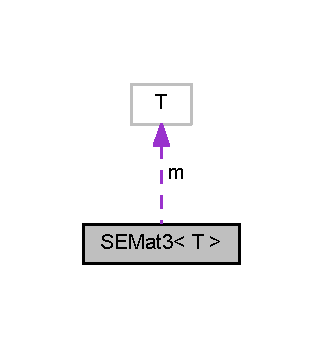
\includegraphics[width=155pt]{class_s_e_mat3__coll__graph}
\end{center}
\end{figure}
\subsection*{Public Member Functions}
\begin{DoxyCompactItemize}
\item 
{\bf S\+E\+Mat3} ()
\item 
{\bf S\+E\+Mat3} (const T \&v)
\item 
{\bf S\+E\+Mat3} (const {\bf S\+E\+Vec3}$<$ T $>$ \&v)
\item 
{\bf S\+E\+Mat3} (const T $\ast$c)
\item 
{\bf S\+E\+Mat3} (const T $\ast$$\ast$v)
\item 
{\bf S\+E\+Mat3} (const {\bf S\+E\+Vec3}$<$ T $>$ \&v1, const {\bf S\+E\+Vec3}$<$ T $>$ \&v2, const {\bf S\+E\+Vec3}$<$ T $>$ \&v3)
\item 
{\bf S\+E\+Mat3} (const T \&n00, const T \&n01, const T \&n02, const T \&n10, const T \&n11, const T \&n12, const T \&n20, const T \&n21, const T \&n22)
\item 
{\bf S\+E\+Mat3} (const {\bf S\+E\+Mat3}$<$ T $>$ \&n)
\item 
{\bf $\sim$\+S\+E\+Mat3} ()
\item 
{\bf S\+E\+Mat3}$<$ T $>$ \& {\bf operator=} (const {\bf S\+E\+Mat3}$<$ T $>$ \&n)
\item 
{\bf S\+E\+Mat3}$<$ T $>$ {\bf operator-\/} () const 
\item 
{\bf S\+E\+Mat3}$<$ T $>$ \& {\bf operator+=} (const {\bf S\+E\+Mat3}$<$ T $>$ \&n)
\item 
{\bf S\+E\+Mat3}$<$ T $>$ \& {\bf operator-\/=} (const {\bf S\+E\+Mat3}$<$ T $>$ \&n)
\item 
{\bf S\+E\+Mat3}$<$ T $>$ \& {\bf operator$\ast$=} (const T \&a)
\item 
{\bf S\+E\+Mat3}$<$ T $>$ \& {\bf operator/=} (const T \&a)
\item 
{\bf S\+E\+Mat3}$<$ T $>$ \& {\bf operator$\ast$=} (const {\bf S\+E\+Mat3}$<$ T $>$ \&n)
\item 
T \& {\bf operator[$\,$]} (std\+::size\+\_\+t i)
\item 
T {\bf operator[$\,$]} (std\+::size\+\_\+t i) const 
\item 
bool {\bf operator==} (const {\bf S\+E\+Mat3}$<$ T $>$ \&n) const 
\item 
bool {\bf operator!=} (const {\bf S\+E\+Mat3}$<$ T $>$ \&n) const 
\item 
T {\bf trace} () const 
\item 
T {\bf det} () const 
\item 
T {\bf determinant} () const 
\item 
{\bf S\+E\+Mat3}$<$ T $>$ {\bf transposed} () const 
\item 
{\bf S\+E\+Mat3}$<$ T $>$ {\bf inverse} () const 
\item 
{\bf S\+E\+Mat3}$<$ T $>$ \& {\bf null} ()
\item 
{\bf S\+E\+Mat3}$<$ T $>$ \& {\bf identity} ()
\item 
{\bf S\+E\+Mat3}$<$ T $>$ \& {\bf transpose} ()
\item 
{\bf S\+E\+Mat3}$<$ T $>$ \& {\bf transpose} (const {\bf S\+E\+Mat3}$<$ T $>$ \&{\bf m})
\item 
{\bf S\+E\+Mat3}$<$ T $>$ \& {\bf invert} ()
\item 
{\bf S\+E\+Mat3}$<$ T $>$ \& {\bf invert} (const {\bf S\+E\+Mat3}$<$ T $>$ \&{\bf m})
\item 
{\bf S\+E\+Mat3}$<$ T $>$ \& {\bf set} (const T \&f)
\item 
{\bf S\+E\+Mat3}$<$ T $>$ \& {\bf set} (const {\bf S\+E\+Vec3}$<$ T $>$ \&v)
\item 
{\bf S\+E\+Mat3}$<$ T $>$ \& {\bf set} (const {\bf S\+E\+Vec3}$<$ T $>$ \&v1, const {\bf S\+E\+Vec3}$<$ T $>$ \&v2, const {\bf S\+E\+Vec3}$<$ T $>$ \&v3)
\item 
{\bf S\+E\+Mat3}$<$ T $>$ \& {\bf set} (const T $\ast$c)
\item 
{\bf S\+E\+Mat3}$<$ T $>$ \& {\bf set} (const T $\ast$$\ast$v)
\item 
{\bf S\+E\+Mat3}$<$ T $>$ \& {\bf set} (const {\bf S\+E\+Mat3}$<$ T $>$ \&n)
\item 
{\bf S\+E\+Mat3}$<$ T $>$ \& {\bf set} (const T \&n00, const T \&n01, const T \&n02, const T \&n10, const T \&n11, const T \&n12, const T \&n20, const T \&n21, const T \&n22)
\end{DoxyCompactItemize}
\subsection*{Public Attributes}
\begin{DoxyCompactItemize}
\item 
T {\bf m} [9]
\item 
T \& {\bf m00}
\item 
T \& {\bf m01}
\item 
T \& {\bf m02}
\item 
T \& {\bf m10}
\item 
T \& {\bf m11}
\item 
T \& {\bf m12}
\item 
T \& {\bf m20}
\item 
T \& {\bf m21}
\item 
T \& {\bf m22}
\item 
T $\ast$ {\bf r1}
\item 
T $\ast$ {\bf r2}
\item 
T $\ast$ {\bf r3}
\end{DoxyCompactItemize}
\subsection*{Friends}
\begin{DoxyCompactItemize}
\item 
{\bf S\+E\+Mat3}$<$ T $>$ {\bf operator+} ({\bf S\+E\+Mat3}$<$ T $>$ lhs, {\bf S\+E\+Mat3}$<$ T $>$ const \&rhs)
\item 
{\bf S\+E\+Mat3}$<$ T $>$ {\bf operator-\/} ({\bf S\+E\+Mat3}$<$ T $>$ lhs, {\bf S\+E\+Mat3}$<$ T $>$ const \&rhs)
\item 
{\bf S\+E\+Mat3}$<$ T $>$ {\bf operator$\ast$} ({\bf S\+E\+Mat3}$<$ T $>$ lhs, T const \&rhs)
\item 
{\bf S\+E\+Mat3}$<$ T $>$ {\bf operator$\ast$} (T const \&lhs, {\bf S\+E\+Mat3}$<$ T $>$ rhs)
\item 
{\bf S\+E\+Mat3}$<$ T $>$ {\bf operator$\ast$} ({\bf S\+E\+Mat3}$<$ T $>$ lhs, {\bf S\+E\+Mat3}$<$ T $>$ const \&rhs)
\item 
{\bf S\+E\+Mat3}$<$ T $>$ {\bf operator/} ({\bf S\+E\+Mat3}$<$ T $>$ lhs, T const \&rhs)
\item 
{\bf S\+E\+Vec3}$<$ T $>$ {\bf operator$\ast$} ({\bf S\+E\+Mat3}$<$ T $>$ const \&lhs, {\bf S\+E\+Vec3}$<$ T $>$ const \&rhs)
\item 
std\+::ostream \& {\bf operator$<$$<$} (std\+::ostream \&os, const {\bf S\+E\+Mat3}$<$ T $>$ \&{\bf m})
\end{DoxyCompactItemize}


\subsection{Detailed Description}
\subsubsection*{template$<$class T$>$class S\+E\+Mat3$<$ T $>$}



Definition at line 43 of file S\+E\+Math.\+h.



\subsection{Constructor \& Destructor Documentation}
\index{S\+E\+Mat3@{S\+E\+Mat3}!S\+E\+Mat3@{S\+E\+Mat3}}
\index{S\+E\+Mat3@{S\+E\+Mat3}!S\+E\+Mat3@{S\+E\+Mat3}}
\subsubsection[{S\+E\+Mat3}]{\setlength{\rightskip}{0pt plus 5cm}template$<$class T$>$ {\bf S\+E\+Mat3}$<$ T $>$\+::{\bf S\+E\+Mat3} (
\begin{DoxyParamCaption}
{}
\end{DoxyParamCaption}
)\hspace{0.3cm}{\ttfamily [inline]}}\label{class_s_e_mat3_a16eab03675ef6e8eb6e02b53edea4e58}


Definition at line 798 of file S\+E\+Math.\+h.



Here is the call graph for this function\+:
\nopagebreak
\begin{figure}[H]
\begin{center}
\leavevmode
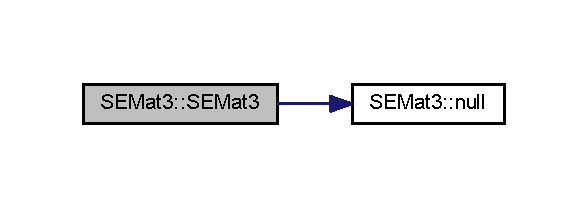
\includegraphics[width=282pt]{class_s_e_mat3_a16eab03675ef6e8eb6e02b53edea4e58_cgraph}
\end{center}
\end{figure}


\index{S\+E\+Mat3@{S\+E\+Mat3}!S\+E\+Mat3@{S\+E\+Mat3}}
\index{S\+E\+Mat3@{S\+E\+Mat3}!S\+E\+Mat3@{S\+E\+Mat3}}
\subsubsection[{S\+E\+Mat3}]{\setlength{\rightskip}{0pt plus 5cm}template$<$class T$>$ {\bf S\+E\+Mat3}$<$ T $>$\+::{\bf S\+E\+Mat3} (
\begin{DoxyParamCaption}
\item[{const T \&}]{v}
\end{DoxyParamCaption}
)\hspace{0.3cm}{\ttfamily [inline]}, {\ttfamily [explicit]}}\label{class_s_e_mat3_a2e3200c79ddfd090d22d175efcd592c4}


Definition at line 805 of file S\+E\+Math.\+h.



Here is the call graph for this function\+:
\nopagebreak
\begin{figure}[H]
\begin{center}
\leavevmode
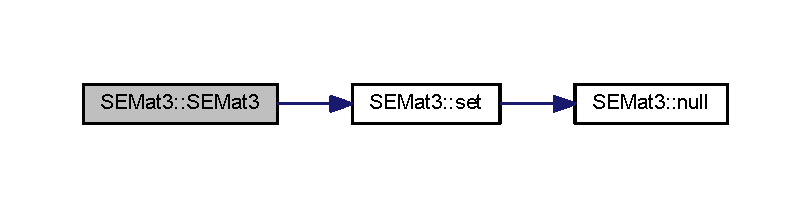
\includegraphics[width=350pt]{class_s_e_mat3_a2e3200c79ddfd090d22d175efcd592c4_cgraph}
\end{center}
\end{figure}


\index{S\+E\+Mat3@{S\+E\+Mat3}!S\+E\+Mat3@{S\+E\+Mat3}}
\index{S\+E\+Mat3@{S\+E\+Mat3}!S\+E\+Mat3@{S\+E\+Mat3}}
\subsubsection[{S\+E\+Mat3}]{\setlength{\rightskip}{0pt plus 5cm}template$<$class T$>$ {\bf S\+E\+Mat3}$<$ T $>$\+::{\bf S\+E\+Mat3} (
\begin{DoxyParamCaption}
\item[{const {\bf S\+E\+Vec3}$<$ T $>$ \&}]{v}
\end{DoxyParamCaption}
)\hspace{0.3cm}{\ttfamily [inline]}, {\ttfamily [explicit]}}\label{class_s_e_mat3_a224ddd964f5fbc91227f1145130c2146}


Definition at line 812 of file S\+E\+Math.\+h.



Here is the call graph for this function\+:
\nopagebreak
\begin{figure}[H]
\begin{center}
\leavevmode
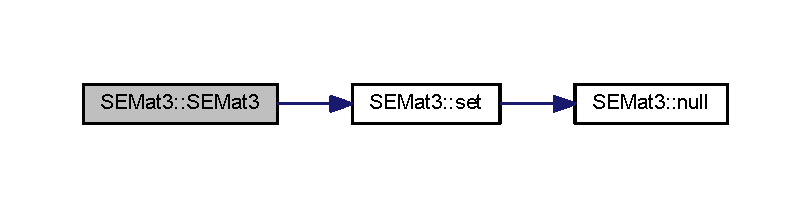
\includegraphics[width=350pt]{class_s_e_mat3_a224ddd964f5fbc91227f1145130c2146_cgraph}
\end{center}
\end{figure}


\index{S\+E\+Mat3@{S\+E\+Mat3}!S\+E\+Mat3@{S\+E\+Mat3}}
\index{S\+E\+Mat3@{S\+E\+Mat3}!S\+E\+Mat3@{S\+E\+Mat3}}
\subsubsection[{S\+E\+Mat3}]{\setlength{\rightskip}{0pt plus 5cm}template$<$class T$>$ {\bf S\+E\+Mat3}$<$ T $>$\+::{\bf S\+E\+Mat3} (
\begin{DoxyParamCaption}
\item[{const T $\ast$}]{c}
\end{DoxyParamCaption}
)\hspace{0.3cm}{\ttfamily [inline]}, {\ttfamily [explicit]}}\label{class_s_e_mat3_a5c475ccea8370bcbe6c9b3e247d53f9b}


Definition at line 819 of file S\+E\+Math.\+h.



Here is the call graph for this function\+:
\nopagebreak
\begin{figure}[H]
\begin{center}
\leavevmode
\includegraphics[width=350pt]{class_s_e_mat3_a5c475ccea8370bcbe6c9b3e247d53f9b_cgraph}
\end{center}
\end{figure}


\index{S\+E\+Mat3@{S\+E\+Mat3}!S\+E\+Mat3@{S\+E\+Mat3}}
\index{S\+E\+Mat3@{S\+E\+Mat3}!S\+E\+Mat3@{S\+E\+Mat3}}
\subsubsection[{S\+E\+Mat3}]{\setlength{\rightskip}{0pt plus 5cm}template$<$class T$>$ {\bf S\+E\+Mat3}$<$ T $>$\+::{\bf S\+E\+Mat3} (
\begin{DoxyParamCaption}
\item[{const T $\ast$$\ast$}]{v}
\end{DoxyParamCaption}
)\hspace{0.3cm}{\ttfamily [inline]}, {\ttfamily [explicit]}}\label{class_s_e_mat3_a910187003b72dd8a2eba0515fa907dc0}


Definition at line 826 of file S\+E\+Math.\+h.



Here is the call graph for this function\+:
\nopagebreak
\begin{figure}[H]
\begin{center}
\leavevmode
\includegraphics[width=350pt]{class_s_e_mat3_a910187003b72dd8a2eba0515fa907dc0_cgraph}
\end{center}
\end{figure}


\index{S\+E\+Mat3@{S\+E\+Mat3}!S\+E\+Mat3@{S\+E\+Mat3}}
\index{S\+E\+Mat3@{S\+E\+Mat3}!S\+E\+Mat3@{S\+E\+Mat3}}
\subsubsection[{S\+E\+Mat3}]{\setlength{\rightskip}{0pt plus 5cm}template$<$class T$>$ {\bf S\+E\+Mat3}$<$ T $>$\+::{\bf S\+E\+Mat3} (
\begin{DoxyParamCaption}
\item[{const {\bf S\+E\+Vec3}$<$ T $>$ \&}]{v1, }
\item[{const {\bf S\+E\+Vec3}$<$ T $>$ \&}]{v2, }
\item[{const {\bf S\+E\+Vec3}$<$ T $>$ \&}]{v3}
\end{DoxyParamCaption}
)\hspace{0.3cm}{\ttfamily [inline]}}\label{class_s_e_mat3_a3acab101b37f8256de9a938efd76e2cf}


Definition at line 833 of file S\+E\+Math.\+h.



Here is the call graph for this function\+:
\nopagebreak
\begin{figure}[H]
\begin{center}
\leavevmode
\includegraphics[width=350pt]{class_s_e_mat3_a3acab101b37f8256de9a938efd76e2cf_cgraph}
\end{center}
\end{figure}


\index{S\+E\+Mat3@{S\+E\+Mat3}!S\+E\+Mat3@{S\+E\+Mat3}}
\index{S\+E\+Mat3@{S\+E\+Mat3}!S\+E\+Mat3@{S\+E\+Mat3}}
\subsubsection[{S\+E\+Mat3}]{\setlength{\rightskip}{0pt plus 5cm}template$<$class T$>$ {\bf S\+E\+Mat3}$<$ T $>$\+::{\bf S\+E\+Mat3} (
\begin{DoxyParamCaption}
\item[{const T \&}]{n00, }
\item[{const T \&}]{n01, }
\item[{const T \&}]{n02, }
\item[{const T \&}]{n10, }
\item[{const T \&}]{n11, }
\item[{const T \&}]{n12, }
\item[{const T \&}]{n20, }
\item[{const T \&}]{n21, }
\item[{const T \&}]{n22}
\end{DoxyParamCaption}
)\hspace{0.3cm}{\ttfamily [inline]}}\label{class_s_e_mat3_a75f6eea3b97238af6c75ed591ea7f33c}


Definition at line 840 of file S\+E\+Math.\+h.



Here is the call graph for this function\+:
\nopagebreak
\begin{figure}[H]
\begin{center}
\leavevmode
\includegraphics[width=350pt]{class_s_e_mat3_a75f6eea3b97238af6c75ed591ea7f33c_cgraph}
\end{center}
\end{figure}


\index{S\+E\+Mat3@{S\+E\+Mat3}!S\+E\+Mat3@{S\+E\+Mat3}}
\index{S\+E\+Mat3@{S\+E\+Mat3}!S\+E\+Mat3@{S\+E\+Mat3}}
\subsubsection[{S\+E\+Mat3}]{\setlength{\rightskip}{0pt plus 5cm}template$<$class T$>$ {\bf S\+E\+Mat3}$<$ T $>$\+::{\bf S\+E\+Mat3} (
\begin{DoxyParamCaption}
\item[{const {\bf S\+E\+Mat3}$<$ T $>$ \&}]{n}
\end{DoxyParamCaption}
)\hspace{0.3cm}{\ttfamily [inline]}}\label{class_s_e_mat3_a6a6d667babce171d008e53791552ffee}


Definition at line 849 of file S\+E\+Math.\+h.



Here is the call graph for this function\+:
\nopagebreak
\begin{figure}[H]
\begin{center}
\leavevmode
\includegraphics[width=350pt]{class_s_e_mat3_a6a6d667babce171d008e53791552ffee_cgraph}
\end{center}
\end{figure}


\index{S\+E\+Mat3@{S\+E\+Mat3}!````~S\+E\+Mat3@{$\sim$\+S\+E\+Mat3}}
\index{````~S\+E\+Mat3@{$\sim$\+S\+E\+Mat3}!S\+E\+Mat3@{S\+E\+Mat3}}
\subsubsection[{$\sim$\+S\+E\+Mat3}]{\setlength{\rightskip}{0pt plus 5cm}template$<$class T$>$ {\bf S\+E\+Mat3}$<$ T $>$\+::$\sim${\bf S\+E\+Mat3} (
\begin{DoxyParamCaption}
{}
\end{DoxyParamCaption}
)\hspace{0.3cm}{\ttfamily [inline]}}\label{class_s_e_mat3_a268f55dc134bf2d7134ac6e902be284b}


Definition at line 856 of file S\+E\+Math.\+h.



\subsection{Member Function Documentation}
\index{S\+E\+Mat3@{S\+E\+Mat3}!det@{det}}
\index{det@{det}!S\+E\+Mat3@{S\+E\+Mat3}}
\subsubsection[{det}]{\setlength{\rightskip}{0pt plus 5cm}template$<$class T$>$ T {\bf S\+E\+Mat3}$<$ T $>$\+::det (
\begin{DoxyParamCaption}
{}
\end{DoxyParamCaption}
) const\hspace{0.3cm}{\ttfamily [inline]}}\label{class_s_e_mat3_ac75564a51747b1e028b213468a2b94ef}


Definition at line 887 of file S\+E\+Math.\+h.

\index{S\+E\+Mat3@{S\+E\+Mat3}!determinant@{determinant}}
\index{determinant@{determinant}!S\+E\+Mat3@{S\+E\+Mat3}}
\subsubsection[{determinant}]{\setlength{\rightskip}{0pt plus 5cm}template$<$class T$>$ T {\bf S\+E\+Mat3}$<$ T $>$\+::determinant (
\begin{DoxyParamCaption}
{}
\end{DoxyParamCaption}
) const\hspace{0.3cm}{\ttfamily [inline]}}\label{class_s_e_mat3_a1401312fa52050d592359a386cc6637e}


Definition at line 888 of file S\+E\+Math.\+h.



Here is the call graph for this function\+:
\nopagebreak
\begin{figure}[H]
\begin{center}
\leavevmode
\includegraphics[width=296pt]{class_s_e_mat3_a1401312fa52050d592359a386cc6637e_cgraph}
\end{center}
\end{figure}


\index{S\+E\+Mat3@{S\+E\+Mat3}!identity@{identity}}
\index{identity@{identity}!S\+E\+Mat3@{S\+E\+Mat3}}
\subsubsection[{identity}]{\setlength{\rightskip}{0pt plus 5cm}template$<$class T$>$ {\bf S\+E\+Mat3}$<$T$>$\& {\bf S\+E\+Mat3}$<$ T $>$\+::identity (
\begin{DoxyParamCaption}
{}
\end{DoxyParamCaption}
)\hspace{0.3cm}{\ttfamily [inline]}}\label{class_s_e_mat3_a5ec3d4bae0e30f40550782f8b2d56f6a}


Definition at line 894 of file S\+E\+Math.\+h.



Here is the call graph for this function\+:
\nopagebreak
\begin{figure}[H]
\begin{center}
\leavevmode
\includegraphics[width=278pt]{class_s_e_mat3_a5ec3d4bae0e30f40550782f8b2d56f6a_cgraph}
\end{center}
\end{figure}


\index{S\+E\+Mat3@{S\+E\+Mat3}!inverse@{inverse}}
\index{inverse@{inverse}!S\+E\+Mat3@{S\+E\+Mat3}}
\subsubsection[{inverse}]{\setlength{\rightskip}{0pt plus 5cm}template$<$class T$>$ {\bf S\+E\+Mat3}$<$T$>$ {\bf S\+E\+Mat3}$<$ T $>$\+::inverse (
\begin{DoxyParamCaption}
{}
\end{DoxyParamCaption}
) const\hspace{0.3cm}{\ttfamily [inline]}}\label{class_s_e_mat3_afa718eb21619c1b52e4bf522098afc7c}


Definition at line 891 of file S\+E\+Math.\+h.



Here is the call graph for this function\+:
\nopagebreak
\begin{figure}[H]
\begin{center}
\leavevmode
\includegraphics[width=350pt]{class_s_e_mat3_afa718eb21619c1b52e4bf522098afc7c_cgraph}
\end{center}
\end{figure}


\index{S\+E\+Mat3@{S\+E\+Mat3}!invert@{invert}}
\index{invert@{invert}!S\+E\+Mat3@{S\+E\+Mat3}}
\subsubsection[{invert}]{\setlength{\rightskip}{0pt plus 5cm}template$<$class T$>$ {\bf S\+E\+Mat3}$<$T$>$\& {\bf S\+E\+Mat3}$<$ T $>$\+::invert (
\begin{DoxyParamCaption}
{}
\end{DoxyParamCaption}
)\hspace{0.3cm}{\ttfamily [inline]}}\label{class_s_e_mat3_a486d1829a395341a99dccb59fcdf0dcb}


Definition at line 897 of file S\+E\+Math.\+h.



Here is the call graph for this function\+:
\nopagebreak
\begin{figure}[H]
\begin{center}
\leavevmode
\includegraphics[width=350pt]{class_s_e_mat3_a486d1829a395341a99dccb59fcdf0dcb_cgraph}
\end{center}
\end{figure}


\index{S\+E\+Mat3@{S\+E\+Mat3}!invert@{invert}}
\index{invert@{invert}!S\+E\+Mat3@{S\+E\+Mat3}}
\subsubsection[{invert}]{\setlength{\rightskip}{0pt plus 5cm}template$<$class T$>$ {\bf S\+E\+Mat3}$<$T$>$\& {\bf S\+E\+Mat3}$<$ T $>$\+::invert (
\begin{DoxyParamCaption}
\item[{const {\bf S\+E\+Mat3}$<$ T $>$ \&}]{m}
\end{DoxyParamCaption}
)\hspace{0.3cm}{\ttfamily [inline]}}\label{class_s_e_mat3_a39f388d4454e28074c7e5d0dc8a92ec8}


Definition at line 916 of file S\+E\+Math.\+h.



Here is the call graph for this function\+:
\nopagebreak
\begin{figure}[H]
\begin{center}
\leavevmode
\includegraphics[width=160pt]{class_s_e_mat3_a39f388d4454e28074c7e5d0dc8a92ec8_cgraph}
\end{center}
\end{figure}


\index{S\+E\+Mat3@{S\+E\+Mat3}!null@{null}}
\index{null@{null}!S\+E\+Mat3@{S\+E\+Mat3}}
\subsubsection[{null}]{\setlength{\rightskip}{0pt plus 5cm}template$<$class T$>$ {\bf S\+E\+Mat3}$<$T$>$\& {\bf S\+E\+Mat3}$<$ T $>$\+::null (
\begin{DoxyParamCaption}
{}
\end{DoxyParamCaption}
)\hspace{0.3cm}{\ttfamily [inline]}}\label{class_s_e_mat3_a04a145f46f4c1f223ca7a5eaab8a2ac8}


Definition at line 893 of file S\+E\+Math.\+h.

\index{S\+E\+Mat3@{S\+E\+Mat3}!operator"!=@{operator"!=}}
\index{operator"!=@{operator"!=}!S\+E\+Mat3@{S\+E\+Mat3}}
\subsubsection[{operator"!=}]{\setlength{\rightskip}{0pt plus 5cm}template$<$class T$>$ bool {\bf S\+E\+Mat3}$<$ T $>$\+::operator!= (
\begin{DoxyParamCaption}
\item[{const {\bf S\+E\+Mat3}$<$ T $>$ \&}]{n}
\end{DoxyParamCaption}
) const\hspace{0.3cm}{\ttfamily [inline]}}\label{class_s_e_mat3_a7e74a058a8ad95df520b047f243a9aba}


Definition at line 882 of file S\+E\+Math.\+h.

\index{S\+E\+Mat3@{S\+E\+Mat3}!operator$\ast$=@{operator$\ast$=}}
\index{operator$\ast$=@{operator$\ast$=}!S\+E\+Mat3@{S\+E\+Mat3}}
\subsubsection[{operator$\ast$=}]{\setlength{\rightskip}{0pt plus 5cm}template$<$class T$>$ {\bf S\+E\+Mat3}$<$T$>$\& {\bf S\+E\+Mat3}$<$ T $>$\+::operator$\ast$= (
\begin{DoxyParamCaption}
\item[{const T \&}]{a}
\end{DoxyParamCaption}
)\hspace{0.3cm}{\ttfamily [inline]}}\label{class_s_e_mat3_acfdf73c34fe7f1db280f5366dc734db9}


Definition at line 863 of file S\+E\+Math.\+h.

\index{S\+E\+Mat3@{S\+E\+Mat3}!operator$\ast$=@{operator$\ast$=}}
\index{operator$\ast$=@{operator$\ast$=}!S\+E\+Mat3@{S\+E\+Mat3}}
\subsubsection[{operator$\ast$=}]{\setlength{\rightskip}{0pt plus 5cm}template$<$class T$>$ {\bf S\+E\+Mat3}$<$T$>$\& {\bf S\+E\+Mat3}$<$ T $>$\+::operator$\ast$= (
\begin{DoxyParamCaption}
\item[{const {\bf S\+E\+Mat3}$<$ T $>$ \&}]{n}
\end{DoxyParamCaption}
)\hspace{0.3cm}{\ttfamily [inline]}}\label{class_s_e_mat3_a669a3d1c59bb27553ed754d6f57a486a}


Definition at line 866 of file S\+E\+Math.\+h.



Here is the call graph for this function\+:
\nopagebreak
\begin{figure}[H]
\begin{center}
\leavevmode
\includegraphics[width=350pt]{class_s_e_mat3_a669a3d1c59bb27553ed754d6f57a486a_cgraph}
\end{center}
\end{figure}


\index{S\+E\+Mat3@{S\+E\+Mat3}!operator+=@{operator+=}}
\index{operator+=@{operator+=}!S\+E\+Mat3@{S\+E\+Mat3}}
\subsubsection[{operator+=}]{\setlength{\rightskip}{0pt plus 5cm}template$<$class T$>$ {\bf S\+E\+Mat3}$<$T$>$\& {\bf S\+E\+Mat3}$<$ T $>$\+::operator+= (
\begin{DoxyParamCaption}
\item[{const {\bf S\+E\+Mat3}$<$ T $>$ \&}]{n}
\end{DoxyParamCaption}
)\hspace{0.3cm}{\ttfamily [inline]}}\label{class_s_e_mat3_ad079706e7d6daa3271f7c873afee66d0}


Definition at line 861 of file S\+E\+Math.\+h.

\index{S\+E\+Mat3@{S\+E\+Mat3}!operator-\/@{operator-\/}}
\index{operator-\/@{operator-\/}!S\+E\+Mat3@{S\+E\+Mat3}}
\subsubsection[{operator-\/}]{\setlength{\rightskip}{0pt plus 5cm}template$<$class T$>$ {\bf S\+E\+Mat3}$<$T$>$ {\bf S\+E\+Mat3}$<$ T $>$\+::operator-\/ (
\begin{DoxyParamCaption}
{}
\end{DoxyParamCaption}
) const\hspace{0.3cm}{\ttfamily [inline]}}\label{class_s_e_mat3_a74f18731406860eea615782261cab354}


Definition at line 859 of file S\+E\+Math.\+h.

\index{S\+E\+Mat3@{S\+E\+Mat3}!operator-\/=@{operator-\/=}}
\index{operator-\/=@{operator-\/=}!S\+E\+Mat3@{S\+E\+Mat3}}
\subsubsection[{operator-\/=}]{\setlength{\rightskip}{0pt plus 5cm}template$<$class T$>$ {\bf S\+E\+Mat3}$<$T$>$\& {\bf S\+E\+Mat3}$<$ T $>$\+::operator-\/= (
\begin{DoxyParamCaption}
\item[{const {\bf S\+E\+Mat3}$<$ T $>$ \&}]{n}
\end{DoxyParamCaption}
)\hspace{0.3cm}{\ttfamily [inline]}}\label{class_s_e_mat3_aa652048db000e7c303e698066f420398}


Definition at line 862 of file S\+E\+Math.\+h.

\index{S\+E\+Mat3@{S\+E\+Mat3}!operator/=@{operator/=}}
\index{operator/=@{operator/=}!S\+E\+Mat3@{S\+E\+Mat3}}
\subsubsection[{operator/=}]{\setlength{\rightskip}{0pt plus 5cm}template$<$class T$>$ {\bf S\+E\+Mat3}$<$T$>$\& {\bf S\+E\+Mat3}$<$ T $>$\+::operator/= (
\begin{DoxyParamCaption}
\item[{const T \&}]{a}
\end{DoxyParamCaption}
)\hspace{0.3cm}{\ttfamily [inline]}}\label{class_s_e_mat3_aceb9d4973460d22748e7df42685695b4}


Definition at line 864 of file S\+E\+Math.\+h.

\index{S\+E\+Mat3@{S\+E\+Mat3}!operator=@{operator=}}
\index{operator=@{operator=}!S\+E\+Mat3@{S\+E\+Mat3}}
\subsubsection[{operator=}]{\setlength{\rightskip}{0pt plus 5cm}template$<$class T$>$ {\bf S\+E\+Mat3}$<$T$>$\& {\bf S\+E\+Mat3}$<$ T $>$\+::operator= (
\begin{DoxyParamCaption}
\item[{const {\bf S\+E\+Mat3}$<$ T $>$ \&}]{n}
\end{DoxyParamCaption}
)\hspace{0.3cm}{\ttfamily [inline]}}\label{class_s_e_mat3_a98b6eeafae5aee343f23543a17fe0f8c}


Definition at line 858 of file S\+E\+Math.\+h.



Here is the call graph for this function\+:
\nopagebreak
\begin{figure}[H]
\begin{center}
\leavevmode
\includegraphics[width=350pt]{class_s_e_mat3_a98b6eeafae5aee343f23543a17fe0f8c_cgraph}
\end{center}
\end{figure}


\index{S\+E\+Mat3@{S\+E\+Mat3}!operator==@{operator==}}
\index{operator==@{operator==}!S\+E\+Mat3@{S\+E\+Mat3}}
\subsubsection[{operator==}]{\setlength{\rightskip}{0pt plus 5cm}template$<$class T$>$ bool {\bf S\+E\+Mat3}$<$ T $>$\+::operator== (
\begin{DoxyParamCaption}
\item[{const {\bf S\+E\+Mat3}$<$ T $>$ \&}]{n}
\end{DoxyParamCaption}
) const\hspace{0.3cm}{\ttfamily [inline]}}\label{class_s_e_mat3_a7a7b892b1bbf56af5137ed5d415c558f}


Definition at line 881 of file S\+E\+Math.\+h.

\index{S\+E\+Mat3@{S\+E\+Mat3}!operator[$\,$]@{operator[]}}
\index{operator[$\,$]@{operator[]}!S\+E\+Mat3@{S\+E\+Mat3}}
\subsubsection[{operator[]}]{\setlength{\rightskip}{0pt plus 5cm}template$<$class T$>$ T\& {\bf S\+E\+Mat3}$<$ T $>$\+::operator[$\,$] (
\begin{DoxyParamCaption}
\item[{std\+::size\+\_\+t}]{i}
\end{DoxyParamCaption}
)\hspace{0.3cm}{\ttfamily [inline]}}\label{class_s_e_mat3_aaf0d2a1df6bf578e41886f1da6cd8b13}


Definition at line 878 of file S\+E\+Math.\+h.

\index{S\+E\+Mat3@{S\+E\+Mat3}!operator[$\,$]@{operator[]}}
\index{operator[$\,$]@{operator[]}!S\+E\+Mat3@{S\+E\+Mat3}}
\subsubsection[{operator[]}]{\setlength{\rightskip}{0pt plus 5cm}template$<$class T$>$ T {\bf S\+E\+Mat3}$<$ T $>$\+::operator[$\,$] (
\begin{DoxyParamCaption}
\item[{std\+::size\+\_\+t}]{i}
\end{DoxyParamCaption}
) const\hspace{0.3cm}{\ttfamily [inline]}}\label{class_s_e_mat3_ac14e0f6a135abd9c06cb8612e4fd1c4f}


Definition at line 879 of file S\+E\+Math.\+h.

\index{S\+E\+Mat3@{S\+E\+Mat3}!set@{set}}
\index{set@{set}!S\+E\+Mat3@{S\+E\+Mat3}}
\subsubsection[{set}]{\setlength{\rightskip}{0pt plus 5cm}template$<$class T$>$ {\bf S\+E\+Mat3}$<$T$>$\& {\bf S\+E\+Mat3}$<$ T $>$\+::set (
\begin{DoxyParamCaption}
\item[{const T \&}]{f}
\end{DoxyParamCaption}
)\hspace{0.3cm}{\ttfamily [inline]}}\label{class_s_e_mat3_aeacf5c781bd7492874db78b10c2b7b82}


Definition at line 919 of file S\+E\+Math.\+h.



Here is the call graph for this function\+:
\nopagebreak
\begin{figure}[H]
\begin{center}
\leavevmode
\includegraphics[width=260pt]{class_s_e_mat3_aeacf5c781bd7492874db78b10c2b7b82_cgraph}
\end{center}
\end{figure}


\index{S\+E\+Mat3@{S\+E\+Mat3}!set@{set}}
\index{set@{set}!S\+E\+Mat3@{S\+E\+Mat3}}
\subsubsection[{set}]{\setlength{\rightskip}{0pt plus 5cm}template$<$class T$>$ {\bf S\+E\+Mat3}$<$T$>$\& {\bf S\+E\+Mat3}$<$ T $>$\+::set (
\begin{DoxyParamCaption}
\item[{const {\bf S\+E\+Vec3}$<$ T $>$ \&}]{v}
\end{DoxyParamCaption}
)\hspace{0.3cm}{\ttfamily [inline]}}\label{class_s_e_mat3_a8a3ac23c0d77bc601991851d961596d3}


Definition at line 920 of file S\+E\+Math.\+h.



Here is the call graph for this function\+:
\nopagebreak
\begin{figure}[H]
\begin{center}
\leavevmode
\includegraphics[width=260pt]{class_s_e_mat3_a8a3ac23c0d77bc601991851d961596d3_cgraph}
\end{center}
\end{figure}


\index{S\+E\+Mat3@{S\+E\+Mat3}!set@{set}}
\index{set@{set}!S\+E\+Mat3@{S\+E\+Mat3}}
\subsubsection[{set}]{\setlength{\rightskip}{0pt plus 5cm}template$<$class T$>$ {\bf S\+E\+Mat3}$<$T$>$\& {\bf S\+E\+Mat3}$<$ T $>$\+::set (
\begin{DoxyParamCaption}
\item[{const {\bf S\+E\+Vec3}$<$ T $>$ \&}]{v1, }
\item[{const {\bf S\+E\+Vec3}$<$ T $>$ \&}]{v2, }
\item[{const {\bf S\+E\+Vec3}$<$ T $>$ \&}]{v3}
\end{DoxyParamCaption}
)\hspace{0.3cm}{\ttfamily [inline]}}\label{class_s_e_mat3_aabc4742961b4a1a588d82b8fd13a97e6}


Definition at line 921 of file S\+E\+Math.\+h.

\index{S\+E\+Mat3@{S\+E\+Mat3}!set@{set}}
\index{set@{set}!S\+E\+Mat3@{S\+E\+Mat3}}
\subsubsection[{set}]{\setlength{\rightskip}{0pt plus 5cm}template$<$class T$>$ {\bf S\+E\+Mat3}$<$T$>$\& {\bf S\+E\+Mat3}$<$ T $>$\+::set (
\begin{DoxyParamCaption}
\item[{const T $\ast$}]{c}
\end{DoxyParamCaption}
)\hspace{0.3cm}{\ttfamily [inline]}}\label{class_s_e_mat3_a6a61ae554938364be40943c494edb775}


Definition at line 922 of file S\+E\+Math.\+h.

\index{S\+E\+Mat3@{S\+E\+Mat3}!set@{set}}
\index{set@{set}!S\+E\+Mat3@{S\+E\+Mat3}}
\subsubsection[{set}]{\setlength{\rightskip}{0pt plus 5cm}template$<$class T$>$ {\bf S\+E\+Mat3}$<$T$>$\& {\bf S\+E\+Mat3}$<$ T $>$\+::set (
\begin{DoxyParamCaption}
\item[{const T $\ast$$\ast$}]{v}
\end{DoxyParamCaption}
)\hspace{0.3cm}{\ttfamily [inline]}}\label{class_s_e_mat3_aa68d6bbc8fbd1600abad9ec295f3769f}


Definition at line 923 of file S\+E\+Math.\+h.

\index{S\+E\+Mat3@{S\+E\+Mat3}!set@{set}}
\index{set@{set}!S\+E\+Mat3@{S\+E\+Mat3}}
\subsubsection[{set}]{\setlength{\rightskip}{0pt plus 5cm}template$<$class T$>$ {\bf S\+E\+Mat3}$<$T$>$\& {\bf S\+E\+Mat3}$<$ T $>$\+::set (
\begin{DoxyParamCaption}
\item[{const {\bf S\+E\+Mat3}$<$ T $>$ \&}]{n}
\end{DoxyParamCaption}
)\hspace{0.3cm}{\ttfamily [inline]}}\label{class_s_e_mat3_a1d2ad7f756a39140ee718c588ee37198}


Definition at line 924 of file S\+E\+Math.\+h.

\index{S\+E\+Mat3@{S\+E\+Mat3}!set@{set}}
\index{set@{set}!S\+E\+Mat3@{S\+E\+Mat3}}
\subsubsection[{set}]{\setlength{\rightskip}{0pt plus 5cm}template$<$class T$>$ {\bf S\+E\+Mat3}$<$T$>$\& {\bf S\+E\+Mat3}$<$ T $>$\+::set (
\begin{DoxyParamCaption}
\item[{const T \&}]{n00, }
\item[{const T \&}]{n01, }
\item[{const T \&}]{n02, }
\item[{const T \&}]{n10, }
\item[{const T \&}]{n11, }
\item[{const T \&}]{n12, }
\item[{const T \&}]{n20, }
\item[{const T \&}]{n21, }
\item[{const T \&}]{n22}
\end{DoxyParamCaption}
)\hspace{0.3cm}{\ttfamily [inline]}}\label{class_s_e_mat3_aeba2ede962491205a0fd1a4063318cfc}


Definition at line 925 of file S\+E\+Math.\+h.

\index{S\+E\+Mat3@{S\+E\+Mat3}!trace@{trace}}
\index{trace@{trace}!S\+E\+Mat3@{S\+E\+Mat3}}
\subsubsection[{trace}]{\setlength{\rightskip}{0pt plus 5cm}template$<$class T$>$ T {\bf S\+E\+Mat3}$<$ T $>$\+::trace (
\begin{DoxyParamCaption}
{}
\end{DoxyParamCaption}
) const\hspace{0.3cm}{\ttfamily [inline]}}\label{class_s_e_mat3_ae3d01f41c34aa1e589ee1646905c1c04}


Definition at line 886 of file S\+E\+Math.\+h.

\index{S\+E\+Mat3@{S\+E\+Mat3}!transpose@{transpose}}
\index{transpose@{transpose}!S\+E\+Mat3@{S\+E\+Mat3}}
\subsubsection[{transpose}]{\setlength{\rightskip}{0pt plus 5cm}template$<$class T$>$ {\bf S\+E\+Mat3}$<$T$>$\& {\bf S\+E\+Mat3}$<$ T $>$\+::transpose (
\begin{DoxyParamCaption}
{}
\end{DoxyParamCaption}
)\hspace{0.3cm}{\ttfamily [inline]}}\label{class_s_e_mat3_acabc1210eabd56ec6499bf0450cdc292}


Definition at line 895 of file S\+E\+Math.\+h.



Here is the call graph for this function\+:
\nopagebreak
\begin{figure}[H]
\begin{center}
\leavevmode
\includegraphics[width=319pt]{class_s_e_mat3_acabc1210eabd56ec6499bf0450cdc292_cgraph}
\end{center}
\end{figure}


\index{S\+E\+Mat3@{S\+E\+Mat3}!transpose@{transpose}}
\index{transpose@{transpose}!S\+E\+Mat3@{S\+E\+Mat3}}
\subsubsection[{transpose}]{\setlength{\rightskip}{0pt plus 5cm}template$<$class T$>$ {\bf S\+E\+Mat3}$<$T$>$\& {\bf S\+E\+Mat3}$<$ T $>$\+::transpose (
\begin{DoxyParamCaption}
\item[{const {\bf S\+E\+Mat3}$<$ T $>$ \&}]{m}
\end{DoxyParamCaption}
)\hspace{0.3cm}{\ttfamily [inline]}}\label{class_s_e_mat3_afe980d968010dd19fe734616fa049519}


Definition at line 896 of file S\+E\+Math.\+h.



Here is the call graph for this function\+:
\nopagebreak
\begin{figure}[H]
\begin{center}
\leavevmode
\includegraphics[width=181pt]{class_s_e_mat3_afe980d968010dd19fe734616fa049519_cgraph}
\end{center}
\end{figure}


\index{S\+E\+Mat3@{S\+E\+Mat3}!transposed@{transposed}}
\index{transposed@{transposed}!S\+E\+Mat3@{S\+E\+Mat3}}
\subsubsection[{transposed}]{\setlength{\rightskip}{0pt plus 5cm}template$<$class T$>$ {\bf S\+E\+Mat3}$<$T$>$ {\bf S\+E\+Mat3}$<$ T $>$\+::transposed (
\begin{DoxyParamCaption}
{}
\end{DoxyParamCaption}
) const\hspace{0.3cm}{\ttfamily [inline]}}\label{class_s_e_mat3_a87ee73b5ceafeca7646a22ecd916c444}


Definition at line 890 of file S\+E\+Math.\+h.



Here is the call graph for this function\+:
\nopagebreak
\begin{figure}[H]
\begin{center}
\leavevmode
\includegraphics[width=350pt]{class_s_e_mat3_a87ee73b5ceafeca7646a22ecd916c444_cgraph}
\end{center}
\end{figure}




\subsection{Friends And Related Function Documentation}
\index{S\+E\+Mat3@{S\+E\+Mat3}!operator$\ast$@{operator$\ast$}}
\index{operator$\ast$@{operator$\ast$}!S\+E\+Mat3@{S\+E\+Mat3}}
\subsubsection[{operator$\ast$}]{\setlength{\rightskip}{0pt plus 5cm}template$<$class T$>$ {\bf S\+E\+Mat3}$<$T$>$ operator$\ast$ (
\begin{DoxyParamCaption}
\item[{{\bf S\+E\+Mat3}$<$ T $>$}]{lhs, }
\item[{T const \&}]{rhs}
\end{DoxyParamCaption}
)\hspace{0.3cm}{\ttfamily [friend]}}\label{class_s_e_mat3_a20d205007ea8283a2f7732ccf03afd90}


Definition at line 872 of file S\+E\+Math.\+h.

\index{S\+E\+Mat3@{S\+E\+Mat3}!operator$\ast$@{operator$\ast$}}
\index{operator$\ast$@{operator$\ast$}!S\+E\+Mat3@{S\+E\+Mat3}}
\subsubsection[{operator$\ast$}]{\setlength{\rightskip}{0pt plus 5cm}template$<$class T$>$ {\bf S\+E\+Mat3}$<$T$>$ operator$\ast$ (
\begin{DoxyParamCaption}
\item[{T const \&}]{lhs, }
\item[{{\bf S\+E\+Mat3}$<$ T $>$}]{rhs}
\end{DoxyParamCaption}
)\hspace{0.3cm}{\ttfamily [friend]}}\label{class_s_e_mat3_aa8feb7e8b0eeb43be7706b902609dd74}


Definition at line 873 of file S\+E\+Math.\+h.

\index{S\+E\+Mat3@{S\+E\+Mat3}!operator$\ast$@{operator$\ast$}}
\index{operator$\ast$@{operator$\ast$}!S\+E\+Mat3@{S\+E\+Mat3}}
\subsubsection[{operator$\ast$}]{\setlength{\rightskip}{0pt plus 5cm}template$<$class T$>$ {\bf S\+E\+Mat3}$<$T$>$ operator$\ast$ (
\begin{DoxyParamCaption}
\item[{{\bf S\+E\+Mat3}$<$ T $>$}]{lhs, }
\item[{{\bf S\+E\+Mat3}$<$ T $>$ const \&}]{rhs}
\end{DoxyParamCaption}
)\hspace{0.3cm}{\ttfamily [friend]}}\label{class_s_e_mat3_a172da1f43718b05e21a273b717d1303f}


Definition at line 874 of file S\+E\+Math.\+h.

\index{S\+E\+Mat3@{S\+E\+Mat3}!operator$\ast$@{operator$\ast$}}
\index{operator$\ast$@{operator$\ast$}!S\+E\+Mat3@{S\+E\+Mat3}}
\subsubsection[{operator$\ast$}]{\setlength{\rightskip}{0pt plus 5cm}template$<$class T$>$ {\bf S\+E\+Vec3}$<$T$>$ operator$\ast$ (
\begin{DoxyParamCaption}
\item[{{\bf S\+E\+Mat3}$<$ T $>$ const \&}]{lhs, }
\item[{{\bf S\+E\+Vec3}$<$ T $>$ const \&}]{rhs}
\end{DoxyParamCaption}
)\hspace{0.3cm}{\ttfamily [friend]}}\label{class_s_e_mat3_ac213a61ebb2373d14728515f7ecf4c33}


Definition at line 876 of file S\+E\+Math.\+h.

\index{S\+E\+Mat3@{S\+E\+Mat3}!operator+@{operator+}}
\index{operator+@{operator+}!S\+E\+Mat3@{S\+E\+Mat3}}
\subsubsection[{operator+}]{\setlength{\rightskip}{0pt plus 5cm}template$<$class T$>$ {\bf S\+E\+Mat3}$<$T$>$ operator+ (
\begin{DoxyParamCaption}
\item[{{\bf S\+E\+Mat3}$<$ T $>$}]{lhs, }
\item[{{\bf S\+E\+Mat3}$<$ T $>$ const \&}]{rhs}
\end{DoxyParamCaption}
)\hspace{0.3cm}{\ttfamily [friend]}}\label{class_s_e_mat3_aa86fd6e2bbb771698502e6145e28df72}


Definition at line 870 of file S\+E\+Math.\+h.

\index{S\+E\+Mat3@{S\+E\+Mat3}!operator-\/@{operator-\/}}
\index{operator-\/@{operator-\/}!S\+E\+Mat3@{S\+E\+Mat3}}
\subsubsection[{operator-\/}]{\setlength{\rightskip}{0pt plus 5cm}template$<$class T$>$ {\bf S\+E\+Mat3}$<$T$>$ operator-\/ (
\begin{DoxyParamCaption}
\item[{{\bf S\+E\+Mat3}$<$ T $>$}]{lhs, }
\item[{{\bf S\+E\+Mat3}$<$ T $>$ const \&}]{rhs}
\end{DoxyParamCaption}
)\hspace{0.3cm}{\ttfamily [friend]}}\label{class_s_e_mat3_a905ea5e11f53de113641c3d72ac1fbb5}


Definition at line 871 of file S\+E\+Math.\+h.

\index{S\+E\+Mat3@{S\+E\+Mat3}!operator/@{operator/}}
\index{operator/@{operator/}!S\+E\+Mat3@{S\+E\+Mat3}}
\subsubsection[{operator/}]{\setlength{\rightskip}{0pt plus 5cm}template$<$class T$>$ {\bf S\+E\+Mat3}$<$T$>$ operator/ (
\begin{DoxyParamCaption}
\item[{{\bf S\+E\+Mat3}$<$ T $>$}]{lhs, }
\item[{T const \&}]{rhs}
\end{DoxyParamCaption}
)\hspace{0.3cm}{\ttfamily [friend]}}\label{class_s_e_mat3_ae1d5c3f68e805881d703b1c79f4741e3}


Definition at line 875 of file S\+E\+Math.\+h.

\index{S\+E\+Mat3@{S\+E\+Mat3}!operator$<$$<$@{operator$<$$<$}}
\index{operator$<$$<$@{operator$<$$<$}!S\+E\+Mat3@{S\+E\+Mat3}}
\subsubsection[{operator$<$$<$}]{\setlength{\rightskip}{0pt plus 5cm}template$<$class T$>$ std\+::ostream\& operator$<$$<$ (
\begin{DoxyParamCaption}
\item[{std\+::ostream \&}]{os, }
\item[{const {\bf S\+E\+Mat3}$<$ T $>$ \&}]{m}
\end{DoxyParamCaption}
)\hspace{0.3cm}{\ttfamily [friend]}}\label{class_s_e_mat3_afe4539a07c8fdb1b6a1ae19701c359bd}


Definition at line 884 of file S\+E\+Math.\+h.



\subsection{Member Data Documentation}
\index{S\+E\+Mat3@{S\+E\+Mat3}!m@{m}}
\index{m@{m}!S\+E\+Mat3@{S\+E\+Mat3}}
\subsubsection[{m}]{\setlength{\rightskip}{0pt plus 5cm}template$<$class T$>$ T {\bf S\+E\+Mat3}$<$ T $>$\+::m[9]}\label{class_s_e_mat3_aa16f24e4b1ac14e23b3ce7c61585a6e4}


Definition at line 781 of file S\+E\+Math.\+h.

\index{S\+E\+Mat3@{S\+E\+Mat3}!m00@{m00}}
\index{m00@{m00}!S\+E\+Mat3@{S\+E\+Mat3}}
\subsubsection[{m00}]{\setlength{\rightskip}{0pt plus 5cm}template$<$class T$>$ T\& {\bf S\+E\+Mat3}$<$ T $>$\+::m00}\label{class_s_e_mat3_acb95e8c56a4c84ad9c1b038e6315ebc9}


Definition at line 784 of file S\+E\+Math.\+h.

\index{S\+E\+Mat3@{S\+E\+Mat3}!m01@{m01}}
\index{m01@{m01}!S\+E\+Mat3@{S\+E\+Mat3}}
\subsubsection[{m01}]{\setlength{\rightskip}{0pt plus 5cm}template$<$class T$>$ T \& {\bf S\+E\+Mat3}$<$ T $>$\+::m01}\label{class_s_e_mat3_a46289da7eee7693478c861fe58d37253}


Definition at line 784 of file S\+E\+Math.\+h.

\index{S\+E\+Mat3@{S\+E\+Mat3}!m02@{m02}}
\index{m02@{m02}!S\+E\+Mat3@{S\+E\+Mat3}}
\subsubsection[{m02}]{\setlength{\rightskip}{0pt plus 5cm}template$<$class T$>$ T \& {\bf S\+E\+Mat3}$<$ T $>$\+::m02}\label{class_s_e_mat3_a08480b22bc1a2d907ce1aa57c3b48c05}


Definition at line 784 of file S\+E\+Math.\+h.

\index{S\+E\+Mat3@{S\+E\+Mat3}!m10@{m10}}
\index{m10@{m10}!S\+E\+Mat3@{S\+E\+Mat3}}
\subsubsection[{m10}]{\setlength{\rightskip}{0pt plus 5cm}template$<$class T$>$ T \& {\bf S\+E\+Mat3}$<$ T $>$\+::m10}\label{class_s_e_mat3_af08dfc1de04f82fb0de1aa1ac0230b44}


Definition at line 784 of file S\+E\+Math.\+h.

\index{S\+E\+Mat3@{S\+E\+Mat3}!m11@{m11}}
\index{m11@{m11}!S\+E\+Mat3@{S\+E\+Mat3}}
\subsubsection[{m11}]{\setlength{\rightskip}{0pt plus 5cm}template$<$class T$>$ T \& {\bf S\+E\+Mat3}$<$ T $>$\+::m11}\label{class_s_e_mat3_a5bad89d5a58743f1c135ad007bc40616}


Definition at line 784 of file S\+E\+Math.\+h.

\index{S\+E\+Mat3@{S\+E\+Mat3}!m12@{m12}}
\index{m12@{m12}!S\+E\+Mat3@{S\+E\+Mat3}}
\subsubsection[{m12}]{\setlength{\rightskip}{0pt plus 5cm}template$<$class T$>$ T \& {\bf S\+E\+Mat3}$<$ T $>$\+::m12}\label{class_s_e_mat3_acbcfb6e63be28a1e143fc58e91df6644}


Definition at line 784 of file S\+E\+Math.\+h.

\index{S\+E\+Mat3@{S\+E\+Mat3}!m20@{m20}}
\index{m20@{m20}!S\+E\+Mat3@{S\+E\+Mat3}}
\subsubsection[{m20}]{\setlength{\rightskip}{0pt plus 5cm}template$<$class T$>$ T \& {\bf S\+E\+Mat3}$<$ T $>$\+::m20}\label{class_s_e_mat3_adfc42ca3baab784970eaec2df3b1cb26}


Definition at line 784 of file S\+E\+Math.\+h.

\index{S\+E\+Mat3@{S\+E\+Mat3}!m21@{m21}}
\index{m21@{m21}!S\+E\+Mat3@{S\+E\+Mat3}}
\subsubsection[{m21}]{\setlength{\rightskip}{0pt plus 5cm}template$<$class T$>$ T \& {\bf S\+E\+Mat3}$<$ T $>$\+::m21}\label{class_s_e_mat3_a115a55f2f63e949d389da2873d0df24b}


Definition at line 784 of file S\+E\+Math.\+h.

\index{S\+E\+Mat3@{S\+E\+Mat3}!m22@{m22}}
\index{m22@{m22}!S\+E\+Mat3@{S\+E\+Mat3}}
\subsubsection[{m22}]{\setlength{\rightskip}{0pt plus 5cm}template$<$class T$>$ T \& {\bf S\+E\+Mat3}$<$ T $>$\+::m22}\label{class_s_e_mat3_a69c0cfe02caca22ffa7f3663e4cf0022}


Definition at line 784 of file S\+E\+Math.\+h.

\index{S\+E\+Mat3@{S\+E\+Mat3}!r1@{r1}}
\index{r1@{r1}!S\+E\+Mat3@{S\+E\+Mat3}}
\subsubsection[{r1}]{\setlength{\rightskip}{0pt plus 5cm}template$<$class T$>$ T $\ast$ {\bf S\+E\+Mat3}$<$ T $>$\+::r1}\label{class_s_e_mat3_ad9e31557f0ef8dc1e13fe9dc5a1de2a2}


Definition at line 784 of file S\+E\+Math.\+h.

\index{S\+E\+Mat3@{S\+E\+Mat3}!r2@{r2}}
\index{r2@{r2}!S\+E\+Mat3@{S\+E\+Mat3}}
\subsubsection[{r2}]{\setlength{\rightskip}{0pt plus 5cm}template$<$class T$>$ T $\ast$ {\bf S\+E\+Mat3}$<$ T $>$\+::r2}\label{class_s_e_mat3_a78753511b1012420f8892bf3ac2a72c3}


Definition at line 784 of file S\+E\+Math.\+h.

\index{S\+E\+Mat3@{S\+E\+Mat3}!r3@{r3}}
\index{r3@{r3}!S\+E\+Mat3@{S\+E\+Mat3}}
\subsubsection[{r3}]{\setlength{\rightskip}{0pt plus 5cm}template$<$class T$>$ T $\ast$ {\bf S\+E\+Mat3}$<$ T $>$\+::r3}\label{class_s_e_mat3_acff13d72fd63f15ddff1a795d9002e14}


Definition at line 784 of file S\+E\+Math.\+h.



The documentation for this class was generated from the following file\+:\begin{DoxyCompactItemize}
\item 
{\bf S\+E\+Math.\+h}\end{DoxyCompactItemize}

\section{S\+E\+Mat4$<$ T $>$ Class Template Reference}
\label{class_s_e_mat4}\index{S\+E\+Mat4$<$ T $>$@{S\+E\+Mat4$<$ T $>$}}


{\ttfamily \#include $<$S\+E\+Math.\+h$>$}



Collaboration diagram for S\+E\+Mat4$<$ T $>$\+:
\nopagebreak
\begin{figure}[H]
\begin{center}
\leavevmode
\includegraphics[width=155pt]{class_s_e_mat4__coll__graph}
\end{center}
\end{figure}
\subsection*{Public Member Functions}
\begin{DoxyCompactItemize}
\item 
{\bf S\+E\+Mat4} ()
\item 
{\bf S\+E\+Mat4} (const T \&v)
\item 
{\bf S\+E\+Mat4} (const {\bf S\+E\+Vec3}$<$ T $>$ \&v)
\item 
{\bf S\+E\+Mat4} (const {\bf S\+E\+Vec4}$<$ T $>$ \&v)
\item 
{\bf S\+E\+Mat4} (const {\bf S\+E\+Quaternion}$<$ T $>$ \&v)
\item 
{\bf S\+E\+Mat4} (const T $\ast$c)
\item 
{\bf S\+E\+Mat4} (const T $\ast$$\ast$v)
\item 
{\bf S\+E\+Mat4} (const {\bf S\+E\+Vec4}$<$ T $>$ \&v1, const {\bf S\+E\+Vec4}$<$ T $>$ \&v2, const {\bf S\+E\+Vec4}$<$ T $>$ \&v3, const {\bf S\+E\+Vec4}$<$ T $>$ \&v4)
\item 
{\bf S\+E\+Mat4} (const T \&n00, const T \&n01, const T \&n02, const T \&n03, const T \&n10, const T \&n11, const T \&n12, const T \&n13, const T \&n20, const T \&n21, const T \&n22, const T \&n23, const T \&n30, const T \&n31, const T \&n32, const T \&n33)
\item 
{\bf S\+E\+Mat4} (const {\bf S\+E\+Mat4}$<$ T $>$ \&n)
\item 
{\bf $\sim$\+S\+E\+Mat4} ()
\item 
{\bf S\+E\+Mat4}$<$ T $>$ \& {\bf operator=} (const {\bf S\+E\+Mat4}$<$ T $>$ \&n)
\item 
{\bf S\+E\+Mat4}$<$ T $>$ {\bf operator-\/} () const 
\item 
{\bf S\+E\+Mat4}$<$ T $>$ \& {\bf operator+=} (const {\bf S\+E\+Mat4}$<$ T $>$ \&n)
\item 
{\bf S\+E\+Mat4}$<$ T $>$ \& {\bf operator-\/=} (const {\bf S\+E\+Mat4}$<$ T $>$ \&n)
\item 
{\bf S\+E\+Mat4}$<$ T $>$ \& {\bf operator$\ast$=} (const T \&a)
\item 
{\bf S\+E\+Mat4}$<$ T $>$ \& {\bf operator$\ast$=} (const {\bf S\+E\+Mat4}$<$ T $>$ \&n)
\item 
{\bf S\+E\+Mat4}$<$ T $>$ \& {\bf operator/=} (const T \&a)
\item 
T \& {\bf operator[$\,$]} (std\+::size\+\_\+t i)
\item 
T {\bf operator[$\,$]} (std\+::size\+\_\+t i) const 
\item 
bool {\bf operator==} (const {\bf S\+E\+Mat4}$<$ T $>$ \&n) const 
\item 
bool {\bf operator!=} (const {\bf S\+E\+Mat4}$<$ T $>$ \&n) const 
\item 
T {\bf trace} () const 
\item 
T {\bf det} () const 
\item 
T {\bf determinant} () const 
\item 
bool {\bf is\+Affine} () const 
\item 
{\bf S\+E\+Mat4}$<$ T $>$ {\bf transposed} () const 
\item 
{\bf S\+E\+Mat4}$<$ T $>$ {\bf inverse} () const 
\item 
{\bf S\+E\+Mat4}$<$ T $>$ \& {\bf null} ()
\item 
{\bf S\+E\+Mat4}$<$ T $>$ \& {\bf identity} ()
\item 
{\bf S\+E\+Mat4}$<$ T $>$ \& {\bf transpose} ()
\item 
{\bf S\+E\+Mat4}$<$ T $>$ \& {\bf transpose} (const {\bf S\+E\+Mat4}$<$ T $>$ \&{\bf m})
\item 
{\bf S\+E\+Mat4}$<$ T $>$ \& {\bf invert\+Affine} ()
\item 
{\bf S\+E\+Mat4}$<$ T $>$ \& {\bf invert} ()
\item 
{\bf S\+E\+Mat4}$<$ T $>$ \& {\bf invert} (const {\bf S\+E\+Mat4}$<$ T $>$ \&{\bf m})
\item 
{\bf S\+E\+Mat4}$<$ T $>$ \& {\bf set} (const T \&f)
\item 
{\bf S\+E\+Mat4}$<$ T $>$ \& {\bf set} (const {\bf S\+E\+Vec3}$<$ T $>$ \&v)
\item 
{\bf S\+E\+Mat4}$<$ T $>$ \& {\bf set} (const {\bf S\+E\+Vec4}$<$ T $>$ \&v)
\item 
{\bf S\+E\+Mat4}$<$ T $>$ \& {\bf set} (const {\bf S\+E\+Quaternion}$<$ T $>$ \&v)
\item 
{\bf S\+E\+Mat4}$<$ T $>$ \& {\bf set} (const T $\ast$c)
\item 
{\bf S\+E\+Mat4}$<$ T $>$ \& {\bf set} (const T $\ast$$\ast$v)
\item 
{\bf S\+E\+Mat4}$<$ T $>$ \& {\bf set} (const {\bf S\+E\+Mat4}$<$ T $>$ \&n)
\item 
{\bf S\+E\+Mat4}$<$ T $>$ \& {\bf set} (const T \&n00, const T \&n01, const T \&n02, const T \&n03, const T \&n10, const T \&n11, const T \&n12, const T \&n13, const T \&n20, const T \&n21, const T \&n22, const T \&n23, const T \&n30, const T \&n31, const T \&n32, const T \&n33)
\item 
{\bf S\+E\+Quaternion}$<$ T $>$ {\bf to\+Quaternion} ()
\end{DoxyCompactItemize}
\subsection*{Public Attributes}
\begin{DoxyCompactItemize}
\item 
T {\bf m} [16]
\item 
T \& {\bf m00}
\item 
T \& {\bf m01}
\item 
T \& {\bf m02}
\item 
T \& {\bf m03}
\item 
T \& {\bf m10}
\item 
T \& {\bf m11}
\item 
T \& {\bf m12}
\item 
T \& {\bf m13}
\item 
T \& {\bf m20}
\item 
T \& {\bf m21}
\item 
T \& {\bf m22}
\item 
T \& {\bf m23}
\item 
T \& {\bf m30}
\item 
T \& {\bf m31}
\item 
T \& {\bf m32}
\item 
T \& {\bf m33}
\item 
T $\ast$ {\bf r1}
\item 
T $\ast$ {\bf r2}
\item 
T $\ast$ {\bf r3}
\item 
T $\ast$ {\bf r4}
\end{DoxyCompactItemize}
\subsection*{Friends}
\begin{DoxyCompactItemize}
\item 
{\bf S\+E\+Mat4}$<$ T $>$ {\bf operator+} ({\bf S\+E\+Mat4}$<$ T $>$ lhs, {\bf S\+E\+Mat4}$<$ T $>$ const \&rhs)
\item 
{\bf S\+E\+Mat4}$<$ T $>$ {\bf operator-\/} ({\bf S\+E\+Mat4}$<$ T $>$ lhs, {\bf S\+E\+Mat4}$<$ T $>$ const \&rhs)
\item 
{\bf S\+E\+Mat4}$<$ T $>$ {\bf operator$\ast$} ({\bf S\+E\+Mat4}$<$ T $>$ lhs, T const \&rhs)
\item 
{\bf S\+E\+Mat4}$<$ T $>$ {\bf operator$\ast$} (T const \&lhs, {\bf S\+E\+Mat4}$<$ T $>$ rhs)
\item 
{\bf S\+E\+Mat4}$<$ T $>$ {\bf operator$\ast$} ({\bf S\+E\+Mat4}$<$ T $>$ lhs, {\bf S\+E\+Mat4}$<$ T $>$ const \&rhs)
\item 
{\bf S\+E\+Mat4}$<$ T $>$ {\bf operator/} ({\bf S\+E\+Mat4}$<$ T $>$ lhs, T const \&rhs)
\item 
{\bf S\+E\+Vec4}$<$ T $>$ {\bf operator$\ast$} ({\bf S\+E\+Mat4}$<$ T $>$ const \&lhs, {\bf S\+E\+Vec4}$<$ T $>$ const \&rhs)
\item 
std\+::ostream \& {\bf operator$<$$<$} (std\+::ostream \&os, const {\bf S\+E\+Mat4}$<$ T $>$ \&{\bf m})
\end{DoxyCompactItemize}


\subsection{Detailed Description}
\subsubsection*{template$<$class T$>$class S\+E\+Mat4$<$ T $>$}



Definition at line 44 of file S\+E\+Math.\+h.



\subsection{Constructor \& Destructor Documentation}
\index{S\+E\+Mat4@{S\+E\+Mat4}!S\+E\+Mat4@{S\+E\+Mat4}}
\index{S\+E\+Mat4@{S\+E\+Mat4}!S\+E\+Mat4@{S\+E\+Mat4}}
\subsubsection[{S\+E\+Mat4}]{\setlength{\rightskip}{0pt plus 5cm}template$<$class T$>$ {\bf S\+E\+Mat4}$<$ T $>$\+::{\bf S\+E\+Mat4} (
\begin{DoxyParamCaption}
{}
\end{DoxyParamCaption}
)\hspace{0.3cm}{\ttfamily [inline]}}\label{class_s_e_mat4_a6986137d04d9f58793505f799e640e5c}


Definition at line 960 of file S\+E\+Math.\+h.

\index{S\+E\+Mat4@{S\+E\+Mat4}!S\+E\+Mat4@{S\+E\+Mat4}}
\index{S\+E\+Mat4@{S\+E\+Mat4}!S\+E\+Mat4@{S\+E\+Mat4}}
\subsubsection[{S\+E\+Mat4}]{\setlength{\rightskip}{0pt plus 5cm}template$<$class T$>$ {\bf S\+E\+Mat4}$<$ T $>$\+::{\bf S\+E\+Mat4} (
\begin{DoxyParamCaption}
\item[{const T \&}]{v}
\end{DoxyParamCaption}
)\hspace{0.3cm}{\ttfamily [inline]}, {\ttfamily [explicit]}}\label{class_s_e_mat4_a9b20ce374805b5f8ed1ba6ba2958f881}


Definition at line 968 of file S\+E\+Math.\+h.

\index{S\+E\+Mat4@{S\+E\+Mat4}!S\+E\+Mat4@{S\+E\+Mat4}}
\index{S\+E\+Mat4@{S\+E\+Mat4}!S\+E\+Mat4@{S\+E\+Mat4}}
\subsubsection[{S\+E\+Mat4}]{\setlength{\rightskip}{0pt plus 5cm}template$<$class T$>$ {\bf S\+E\+Mat4}$<$ T $>$\+::{\bf S\+E\+Mat4} (
\begin{DoxyParamCaption}
\item[{const {\bf S\+E\+Vec3}$<$ T $>$ \&}]{v}
\end{DoxyParamCaption}
)\hspace{0.3cm}{\ttfamily [inline]}, {\ttfamily [explicit]}}\label{class_s_e_mat4_ac5c45c7a706fc0e1c63ec99bcdfcf2cf}


Definition at line 976 of file S\+E\+Math.\+h.

\index{S\+E\+Mat4@{S\+E\+Mat4}!S\+E\+Mat4@{S\+E\+Mat4}}
\index{S\+E\+Mat4@{S\+E\+Mat4}!S\+E\+Mat4@{S\+E\+Mat4}}
\subsubsection[{S\+E\+Mat4}]{\setlength{\rightskip}{0pt plus 5cm}template$<$class T$>$ {\bf S\+E\+Mat4}$<$ T $>$\+::{\bf S\+E\+Mat4} (
\begin{DoxyParamCaption}
\item[{const {\bf S\+E\+Vec4}$<$ T $>$ \&}]{v}
\end{DoxyParamCaption}
)\hspace{0.3cm}{\ttfamily [inline]}, {\ttfamily [explicit]}}\label{class_s_e_mat4_a8f17b17ad5c431ec0b51220d3d756718}


Definition at line 984 of file S\+E\+Math.\+h.

\index{S\+E\+Mat4@{S\+E\+Mat4}!S\+E\+Mat4@{S\+E\+Mat4}}
\index{S\+E\+Mat4@{S\+E\+Mat4}!S\+E\+Mat4@{S\+E\+Mat4}}
\subsubsection[{S\+E\+Mat4}]{\setlength{\rightskip}{0pt plus 5cm}template$<$class T$>$ {\bf S\+E\+Mat4}$<$ T $>$\+::{\bf S\+E\+Mat4} (
\begin{DoxyParamCaption}
\item[{const {\bf S\+E\+Quaternion}$<$ T $>$ \&}]{v}
\end{DoxyParamCaption}
)\hspace{0.3cm}{\ttfamily [inline]}, {\ttfamily [explicit]}}\label{class_s_e_mat4_ae620d9c5a80b6307f7e0a8bb6338afcd}


Definition at line 992 of file S\+E\+Math.\+h.

\index{S\+E\+Mat4@{S\+E\+Mat4}!S\+E\+Mat4@{S\+E\+Mat4}}
\index{S\+E\+Mat4@{S\+E\+Mat4}!S\+E\+Mat4@{S\+E\+Mat4}}
\subsubsection[{S\+E\+Mat4}]{\setlength{\rightskip}{0pt plus 5cm}template$<$class T$>$ {\bf S\+E\+Mat4}$<$ T $>$\+::{\bf S\+E\+Mat4} (
\begin{DoxyParamCaption}
\item[{const T $\ast$}]{c}
\end{DoxyParamCaption}
)\hspace{0.3cm}{\ttfamily [inline]}, {\ttfamily [explicit]}}\label{class_s_e_mat4_a9f5ea59b5168f2b079f2834d0dc0aff6}


Definition at line 1000 of file S\+E\+Math.\+h.

\index{S\+E\+Mat4@{S\+E\+Mat4}!S\+E\+Mat4@{S\+E\+Mat4}}
\index{S\+E\+Mat4@{S\+E\+Mat4}!S\+E\+Mat4@{S\+E\+Mat4}}
\subsubsection[{S\+E\+Mat4}]{\setlength{\rightskip}{0pt plus 5cm}template$<$class T$>$ {\bf S\+E\+Mat4}$<$ T $>$\+::{\bf S\+E\+Mat4} (
\begin{DoxyParamCaption}
\item[{const T $\ast$$\ast$}]{v}
\end{DoxyParamCaption}
)\hspace{0.3cm}{\ttfamily [inline]}, {\ttfamily [explicit]}}\label{class_s_e_mat4_acb93ac58f8aaf396c94cbcf23511e4ce}


Definition at line 1008 of file S\+E\+Math.\+h.

\index{S\+E\+Mat4@{S\+E\+Mat4}!S\+E\+Mat4@{S\+E\+Mat4}}
\index{S\+E\+Mat4@{S\+E\+Mat4}!S\+E\+Mat4@{S\+E\+Mat4}}
\subsubsection[{S\+E\+Mat4}]{\setlength{\rightskip}{0pt plus 5cm}template$<$class T$>$ {\bf S\+E\+Mat4}$<$ T $>$\+::{\bf S\+E\+Mat4} (
\begin{DoxyParamCaption}
\item[{const {\bf S\+E\+Vec4}$<$ T $>$ \&}]{v1, }
\item[{const {\bf S\+E\+Vec4}$<$ T $>$ \&}]{v2, }
\item[{const {\bf S\+E\+Vec4}$<$ T $>$ \&}]{v3, }
\item[{const {\bf S\+E\+Vec4}$<$ T $>$ \&}]{v4}
\end{DoxyParamCaption}
)\hspace{0.3cm}{\ttfamily [inline]}}\label{class_s_e_mat4_aae6ae3c8bd8004e11ed82e084cfe4638}


Definition at line 1016 of file S\+E\+Math.\+h.

\index{S\+E\+Mat4@{S\+E\+Mat4}!S\+E\+Mat4@{S\+E\+Mat4}}
\index{S\+E\+Mat4@{S\+E\+Mat4}!S\+E\+Mat4@{S\+E\+Mat4}}
\subsubsection[{S\+E\+Mat4}]{\setlength{\rightskip}{0pt plus 5cm}template$<$class T$>$ {\bf S\+E\+Mat4}$<$ T $>$\+::{\bf S\+E\+Mat4} (
\begin{DoxyParamCaption}
\item[{const T \&}]{n00, }
\item[{const T \&}]{n01, }
\item[{const T \&}]{n02, }
\item[{const T \&}]{n03, }
\item[{const T \&}]{n10, }
\item[{const T \&}]{n11, }
\item[{const T \&}]{n12, }
\item[{const T \&}]{n13, }
\item[{const T \&}]{n20, }
\item[{const T \&}]{n21, }
\item[{const T \&}]{n22, }
\item[{const T \&}]{n23, }
\item[{const T \&}]{n30, }
\item[{const T \&}]{n31, }
\item[{const T \&}]{n32, }
\item[{const T \&}]{n33}
\end{DoxyParamCaption}
)\hspace{0.3cm}{\ttfamily [inline]}}\label{class_s_e_mat4_af68811c53226c5aa08bb25806cb5dca6}


Definition at line 1024 of file S\+E\+Math.\+h.

\index{S\+E\+Mat4@{S\+E\+Mat4}!S\+E\+Mat4@{S\+E\+Mat4}}
\index{S\+E\+Mat4@{S\+E\+Mat4}!S\+E\+Mat4@{S\+E\+Mat4}}
\subsubsection[{S\+E\+Mat4}]{\setlength{\rightskip}{0pt plus 5cm}template$<$class T$>$ {\bf S\+E\+Mat4}$<$ T $>$\+::{\bf S\+E\+Mat4} (
\begin{DoxyParamCaption}
\item[{const {\bf S\+E\+Mat4}$<$ T $>$ \&}]{n}
\end{DoxyParamCaption}
)\hspace{0.3cm}{\ttfamily [inline]}}\label{class_s_e_mat4_a2d4752c11a82e98e5d21ce225547356b}


Definition at line 1035 of file S\+E\+Math.\+h.

\index{S\+E\+Mat4@{S\+E\+Mat4}!````~S\+E\+Mat4@{$\sim$\+S\+E\+Mat4}}
\index{````~S\+E\+Mat4@{$\sim$\+S\+E\+Mat4}!S\+E\+Mat4@{S\+E\+Mat4}}
\subsubsection[{$\sim$\+S\+E\+Mat4}]{\setlength{\rightskip}{0pt plus 5cm}template$<$class T$>$ {\bf S\+E\+Mat4}$<$ T $>$\+::$\sim${\bf S\+E\+Mat4} (
\begin{DoxyParamCaption}
{}
\end{DoxyParamCaption}
)\hspace{0.3cm}{\ttfamily [inline]}}\label{class_s_e_mat4_af42fec4594dcc1703da1f62e8fd0161c}


Definition at line 1043 of file S\+E\+Math.\+h.



\subsection{Member Function Documentation}
\index{S\+E\+Mat4@{S\+E\+Mat4}!det@{det}}
\index{det@{det}!S\+E\+Mat4@{S\+E\+Mat4}}
\subsubsection[{det}]{\setlength{\rightskip}{0pt plus 5cm}template$<$class T$>$ T {\bf S\+E\+Mat4}$<$ T $>$\+::det (
\begin{DoxyParamCaption}
{}
\end{DoxyParamCaption}
) const\hspace{0.3cm}{\ttfamily [inline]}}\label{class_s_e_mat4_ab1dbf4cbb8c7718d97f39164f66ef8ec}


Definition at line 1075 of file S\+E\+Math.\+h.

\index{S\+E\+Mat4@{S\+E\+Mat4}!determinant@{determinant}}
\index{determinant@{determinant}!S\+E\+Mat4@{S\+E\+Mat4}}
\subsubsection[{determinant}]{\setlength{\rightskip}{0pt plus 5cm}template$<$class T$>$ T {\bf S\+E\+Mat4}$<$ T $>$\+::determinant (
\begin{DoxyParamCaption}
{}
\end{DoxyParamCaption}
) const\hspace{0.3cm}{\ttfamily [inline]}}\label{class_s_e_mat4_a51e4ace29863ce10532a3dfed3e70f87}


Definition at line 1079 of file S\+E\+Math.\+h.

\index{S\+E\+Mat4@{S\+E\+Mat4}!identity@{identity}}
\index{identity@{identity}!S\+E\+Mat4@{S\+E\+Mat4}}
\subsubsection[{identity}]{\setlength{\rightskip}{0pt plus 5cm}template$<$class T$>$ {\bf S\+E\+Mat4}$<$T$>$\& {\bf S\+E\+Mat4}$<$ T $>$\+::identity (
\begin{DoxyParamCaption}
{}
\end{DoxyParamCaption}
)\hspace{0.3cm}{\ttfamily [inline]}}\label{class_s_e_mat4_abd4e4c3ef45e8e3a01bb1ce531128ce6}


Definition at line 1087 of file S\+E\+Math.\+h.

\index{S\+E\+Mat4@{S\+E\+Mat4}!inverse@{inverse}}
\index{inverse@{inverse}!S\+E\+Mat4@{S\+E\+Mat4}}
\subsubsection[{inverse}]{\setlength{\rightskip}{0pt plus 5cm}template$<$class T$>$ {\bf S\+E\+Mat4}$<$T$>$ {\bf S\+E\+Mat4}$<$ T $>$\+::inverse (
\begin{DoxyParamCaption}
{}
\end{DoxyParamCaption}
) const\hspace{0.3cm}{\ttfamily [inline]}}\label{class_s_e_mat4_ae15ef5e80d8fd8857e6de208b5c7e4a2}


Definition at line 1084 of file S\+E\+Math.\+h.

\index{S\+E\+Mat4@{S\+E\+Mat4}!invert@{invert}}
\index{invert@{invert}!S\+E\+Mat4@{S\+E\+Mat4}}
\subsubsection[{invert}]{\setlength{\rightskip}{0pt plus 5cm}template$<$class T$>$ {\bf S\+E\+Mat4}$<$T$>$\& {\bf S\+E\+Mat4}$<$ T $>$\+::invert (
\begin{DoxyParamCaption}
{}
\end{DoxyParamCaption}
)\hspace{0.3cm}{\ttfamily [inline]}}\label{class_s_e_mat4_a93984cc348c467a68129adc0cc148d2e}


Definition at line 1103 of file S\+E\+Math.\+h.

\index{S\+E\+Mat4@{S\+E\+Mat4}!invert@{invert}}
\index{invert@{invert}!S\+E\+Mat4@{S\+E\+Mat4}}
\subsubsection[{invert}]{\setlength{\rightskip}{0pt plus 5cm}template$<$class T$>$ {\bf S\+E\+Mat4}$<$T$>$\& {\bf S\+E\+Mat4}$<$ T $>$\+::invert (
\begin{DoxyParamCaption}
\item[{const {\bf S\+E\+Mat4}$<$ T $>$ \&}]{m}
\end{DoxyParamCaption}
)\hspace{0.3cm}{\ttfamily [inline]}}\label{class_s_e_mat4_a7013902c825a93d38574a169ed8c1e46}


Definition at line 1134 of file S\+E\+Math.\+h.

\index{S\+E\+Mat4@{S\+E\+Mat4}!invert\+Affine@{invert\+Affine}}
\index{invert\+Affine@{invert\+Affine}!S\+E\+Mat4@{S\+E\+Mat4}}
\subsubsection[{invert\+Affine}]{\setlength{\rightskip}{0pt plus 5cm}template$<$class T$>$ {\bf S\+E\+Mat4}$<$T$>$\& {\bf S\+E\+Mat4}$<$ T $>$\+::invert\+Affine (
\begin{DoxyParamCaption}
{}
\end{DoxyParamCaption}
)\hspace{0.3cm}{\ttfamily [inline]}}\label{class_s_e_mat4_a318766d254e436670312ffee8194f610}


Definition at line 1090 of file S\+E\+Math.\+h.

\index{S\+E\+Mat4@{S\+E\+Mat4}!is\+Affine@{is\+Affine}}
\index{is\+Affine@{is\+Affine}!S\+E\+Mat4@{S\+E\+Mat4}}
\subsubsection[{is\+Affine}]{\setlength{\rightskip}{0pt plus 5cm}template$<$class T$>$ bool {\bf S\+E\+Mat4}$<$ T $>$\+::is\+Affine (
\begin{DoxyParamCaption}
{}
\end{DoxyParamCaption}
) const\hspace{0.3cm}{\ttfamily [inline]}}\label{class_s_e_mat4_a2f03737de43260692f83d4ece4f6c373}


Definition at line 1081 of file S\+E\+Math.\+h.

\index{S\+E\+Mat4@{S\+E\+Mat4}!null@{null}}
\index{null@{null}!S\+E\+Mat4@{S\+E\+Mat4}}
\subsubsection[{null}]{\setlength{\rightskip}{0pt plus 5cm}template$<$class T$>$ {\bf S\+E\+Mat4}$<$T$>$\& {\bf S\+E\+Mat4}$<$ T $>$\+::null (
\begin{DoxyParamCaption}
{}
\end{DoxyParamCaption}
)\hspace{0.3cm}{\ttfamily [inline]}}\label{class_s_e_mat4_ab73ec5bb3a53087d7a912964da1f00d4}


Definition at line 1086 of file S\+E\+Math.\+h.

\index{S\+E\+Mat4@{S\+E\+Mat4}!operator"!=@{operator"!=}}
\index{operator"!=@{operator"!=}!S\+E\+Mat4@{S\+E\+Mat4}}
\subsubsection[{operator"!=}]{\setlength{\rightskip}{0pt plus 5cm}template$<$class T$>$ bool {\bf S\+E\+Mat4}$<$ T $>$\+::operator!= (
\begin{DoxyParamCaption}
\item[{const {\bf S\+E\+Mat4}$<$ T $>$ \&}]{n}
\end{DoxyParamCaption}
) const\hspace{0.3cm}{\ttfamily [inline]}}\label{class_s_e_mat4_a9a6378674510a4ee4cc2de6ea31150c3}


Definition at line 1070 of file S\+E\+Math.\+h.

\index{S\+E\+Mat4@{S\+E\+Mat4}!operator$\ast$=@{operator$\ast$=}}
\index{operator$\ast$=@{operator$\ast$=}!S\+E\+Mat4@{S\+E\+Mat4}}
\subsubsection[{operator$\ast$=}]{\setlength{\rightskip}{0pt plus 5cm}template$<$class T$>$ {\bf S\+E\+Mat4}$<$T$>$\& {\bf S\+E\+Mat4}$<$ T $>$\+::operator$\ast$= (
\begin{DoxyParamCaption}
\item[{const T \&}]{a}
\end{DoxyParamCaption}
)\hspace{0.3cm}{\ttfamily [inline]}}\label{class_s_e_mat4_a4f80dc88ca8528daa357ad83bb367620}


Definition at line 1050 of file S\+E\+Math.\+h.

\index{S\+E\+Mat4@{S\+E\+Mat4}!operator$\ast$=@{operator$\ast$=}}
\index{operator$\ast$=@{operator$\ast$=}!S\+E\+Mat4@{S\+E\+Mat4}}
\subsubsection[{operator$\ast$=}]{\setlength{\rightskip}{0pt plus 5cm}template$<$class T$>$ {\bf S\+E\+Mat4}$<$T$>$\& {\bf S\+E\+Mat4}$<$ T $>$\+::operator$\ast$= (
\begin{DoxyParamCaption}
\item[{const {\bf S\+E\+Mat4}$<$ T $>$ \&}]{n}
\end{DoxyParamCaption}
)\hspace{0.3cm}{\ttfamily [inline]}}\label{class_s_e_mat4_a7ab40c2196aca8407016a622c522b079}


Definition at line 1051 of file S\+E\+Math.\+h.

\index{S\+E\+Mat4@{S\+E\+Mat4}!operator+=@{operator+=}}
\index{operator+=@{operator+=}!S\+E\+Mat4@{S\+E\+Mat4}}
\subsubsection[{operator+=}]{\setlength{\rightskip}{0pt plus 5cm}template$<$class T$>$ {\bf S\+E\+Mat4}$<$T$>$\& {\bf S\+E\+Mat4}$<$ T $>$\+::operator+= (
\begin{DoxyParamCaption}
\item[{const {\bf S\+E\+Mat4}$<$ T $>$ \&}]{n}
\end{DoxyParamCaption}
)\hspace{0.3cm}{\ttfamily [inline]}}\label{class_s_e_mat4_a3074766be0d29f1072a4c2ca5c66843f}


Definition at line 1048 of file S\+E\+Math.\+h.

\index{S\+E\+Mat4@{S\+E\+Mat4}!operator-\/@{operator-\/}}
\index{operator-\/@{operator-\/}!S\+E\+Mat4@{S\+E\+Mat4}}
\subsubsection[{operator-\/}]{\setlength{\rightskip}{0pt plus 5cm}template$<$class T$>$ {\bf S\+E\+Mat4}$<$T$>$ {\bf S\+E\+Mat4}$<$ T $>$\+::operator-\/ (
\begin{DoxyParamCaption}
{}
\end{DoxyParamCaption}
) const\hspace{0.3cm}{\ttfamily [inline]}}\label{class_s_e_mat4_a5a8afdb60c304978f82c72aa681e7ea9}


Definition at line 1046 of file S\+E\+Math.\+h.

\index{S\+E\+Mat4@{S\+E\+Mat4}!operator-\/=@{operator-\/=}}
\index{operator-\/=@{operator-\/=}!S\+E\+Mat4@{S\+E\+Mat4}}
\subsubsection[{operator-\/=}]{\setlength{\rightskip}{0pt plus 5cm}template$<$class T$>$ {\bf S\+E\+Mat4}$<$T$>$\& {\bf S\+E\+Mat4}$<$ T $>$\+::operator-\/= (
\begin{DoxyParamCaption}
\item[{const {\bf S\+E\+Mat4}$<$ T $>$ \&}]{n}
\end{DoxyParamCaption}
)\hspace{0.3cm}{\ttfamily [inline]}}\label{class_s_e_mat4_ae60bbdcf5ac3171a088a5c3904ea24e6}


Definition at line 1049 of file S\+E\+Math.\+h.

\index{S\+E\+Mat4@{S\+E\+Mat4}!operator/=@{operator/=}}
\index{operator/=@{operator/=}!S\+E\+Mat4@{S\+E\+Mat4}}
\subsubsection[{operator/=}]{\setlength{\rightskip}{0pt plus 5cm}template$<$class T$>$ {\bf S\+E\+Mat4}$<$T$>$\& {\bf S\+E\+Mat4}$<$ T $>$\+::operator/= (
\begin{DoxyParamCaption}
\item[{const T \&}]{a}
\end{DoxyParamCaption}
)\hspace{0.3cm}{\ttfamily [inline]}}\label{class_s_e_mat4_aac974983979375f39fe6805893893126}


Definition at line 1056 of file S\+E\+Math.\+h.

\index{S\+E\+Mat4@{S\+E\+Mat4}!operator=@{operator=}}
\index{operator=@{operator=}!S\+E\+Mat4@{S\+E\+Mat4}}
\subsubsection[{operator=}]{\setlength{\rightskip}{0pt plus 5cm}template$<$class T$>$ {\bf S\+E\+Mat4}$<$T$>$\& {\bf S\+E\+Mat4}$<$ T $>$\+::operator= (
\begin{DoxyParamCaption}
\item[{const {\bf S\+E\+Mat4}$<$ T $>$ \&}]{n}
\end{DoxyParamCaption}
)\hspace{0.3cm}{\ttfamily [inline]}}\label{class_s_e_mat4_a5ceedf9836716b871612e75d21a68857}


Definition at line 1045 of file S\+E\+Math.\+h.

\index{S\+E\+Mat4@{S\+E\+Mat4}!operator==@{operator==}}
\index{operator==@{operator==}!S\+E\+Mat4@{S\+E\+Mat4}}
\subsubsection[{operator==}]{\setlength{\rightskip}{0pt plus 5cm}template$<$class T$>$ bool {\bf S\+E\+Mat4}$<$ T $>$\+::operator== (
\begin{DoxyParamCaption}
\item[{const {\bf S\+E\+Mat4}$<$ T $>$ \&}]{n}
\end{DoxyParamCaption}
) const\hspace{0.3cm}{\ttfamily [inline]}}\label{class_s_e_mat4_a3009e4fe878f861b11ba520a2554d794}


Definition at line 1069 of file S\+E\+Math.\+h.

\index{S\+E\+Mat4@{S\+E\+Mat4}!operator[$\,$]@{operator[]}}
\index{operator[$\,$]@{operator[]}!S\+E\+Mat4@{S\+E\+Mat4}}
\subsubsection[{operator[]}]{\setlength{\rightskip}{0pt plus 5cm}template$<$class T$>$ T\& {\bf S\+E\+Mat4}$<$ T $>$\+::operator[$\,$] (
\begin{DoxyParamCaption}
\item[{std\+::size\+\_\+t}]{i}
\end{DoxyParamCaption}
)\hspace{0.3cm}{\ttfamily [inline]}}\label{class_s_e_mat4_a0f30332d0d9f13495afbdfb92ba97f3a}


Definition at line 1066 of file S\+E\+Math.\+h.

\index{S\+E\+Mat4@{S\+E\+Mat4}!operator[$\,$]@{operator[]}}
\index{operator[$\,$]@{operator[]}!S\+E\+Mat4@{S\+E\+Mat4}}
\subsubsection[{operator[]}]{\setlength{\rightskip}{0pt plus 5cm}template$<$class T$>$ T {\bf S\+E\+Mat4}$<$ T $>$\+::operator[$\,$] (
\begin{DoxyParamCaption}
\item[{std\+::size\+\_\+t}]{i}
\end{DoxyParamCaption}
) const\hspace{0.3cm}{\ttfamily [inline]}}\label{class_s_e_mat4_aa34600d396149894444916f3a39ec758}


Definition at line 1067 of file S\+E\+Math.\+h.

\index{S\+E\+Mat4@{S\+E\+Mat4}!set@{set}}
\index{set@{set}!S\+E\+Mat4@{S\+E\+Mat4}}
\subsubsection[{set}]{\setlength{\rightskip}{0pt plus 5cm}template$<$class T$>$ {\bf S\+E\+Mat4}$<$T$>$\& {\bf S\+E\+Mat4}$<$ T $>$\+::set (
\begin{DoxyParamCaption}
\item[{const T \&}]{f}
\end{DoxyParamCaption}
)\hspace{0.3cm}{\ttfamily [inline]}}\label{class_s_e_mat4_a0267f07a8f5b781d01135c724306be26}


Definition at line 1136 of file S\+E\+Math.\+h.

\index{S\+E\+Mat4@{S\+E\+Mat4}!set@{set}}
\index{set@{set}!S\+E\+Mat4@{S\+E\+Mat4}}
\subsubsection[{set}]{\setlength{\rightskip}{0pt plus 5cm}template$<$class T$>$ {\bf S\+E\+Mat4}$<$T$>$\& {\bf S\+E\+Mat4}$<$ T $>$\+::set (
\begin{DoxyParamCaption}
\item[{const {\bf S\+E\+Vec3}$<$ T $>$ \&}]{v}
\end{DoxyParamCaption}
)\hspace{0.3cm}{\ttfamily [inline]}}\label{class_s_e_mat4_ab2973c4ef2d38912ea7b81b41f95c7bf}


Definition at line 1137 of file S\+E\+Math.\+h.

\index{S\+E\+Mat4@{S\+E\+Mat4}!set@{set}}
\index{set@{set}!S\+E\+Mat4@{S\+E\+Mat4}}
\subsubsection[{set}]{\setlength{\rightskip}{0pt plus 5cm}template$<$class T$>$ {\bf S\+E\+Mat4}$<$T$>$\& {\bf S\+E\+Mat4}$<$ T $>$\+::set (
\begin{DoxyParamCaption}
\item[{const {\bf S\+E\+Vec4}$<$ T $>$ \&}]{v}
\end{DoxyParamCaption}
)\hspace{0.3cm}{\ttfamily [inline]}}\label{class_s_e_mat4_a2da1a6738c173abb6185d7240fa566f2}


Definition at line 1138 of file S\+E\+Math.\+h.

\index{S\+E\+Mat4@{S\+E\+Mat4}!set@{set}}
\index{set@{set}!S\+E\+Mat4@{S\+E\+Mat4}}
\subsubsection[{set}]{\setlength{\rightskip}{0pt plus 5cm}template$<$class T$>$ {\bf S\+E\+Mat4}$<$T$>$\& {\bf S\+E\+Mat4}$<$ T $>$\+::set (
\begin{DoxyParamCaption}
\item[{const {\bf S\+E\+Quaternion}$<$ T $>$ \&}]{v}
\end{DoxyParamCaption}
)\hspace{0.3cm}{\ttfamily [inline]}}\label{class_s_e_mat4_a0778671c5b9746e27cc5c0c71ed4e11a}


Definition at line 1139 of file S\+E\+Math.\+h.

\index{S\+E\+Mat4@{S\+E\+Mat4}!set@{set}}
\index{set@{set}!S\+E\+Mat4@{S\+E\+Mat4}}
\subsubsection[{set}]{\setlength{\rightskip}{0pt plus 5cm}template$<$class T$>$ {\bf S\+E\+Mat4}$<$T$>$\& {\bf S\+E\+Mat4}$<$ T $>$\+::set (
\begin{DoxyParamCaption}
\item[{const T $\ast$}]{c}
\end{DoxyParamCaption}
)\hspace{0.3cm}{\ttfamily [inline]}}\label{class_s_e_mat4_a064a202d4dab963d3389173b49c983da}


Definition at line 1140 of file S\+E\+Math.\+h.

\index{S\+E\+Mat4@{S\+E\+Mat4}!set@{set}}
\index{set@{set}!S\+E\+Mat4@{S\+E\+Mat4}}
\subsubsection[{set}]{\setlength{\rightskip}{0pt plus 5cm}template$<$class T$>$ {\bf S\+E\+Mat4}$<$T$>$\& {\bf S\+E\+Mat4}$<$ T $>$\+::set (
\begin{DoxyParamCaption}
\item[{const T $\ast$$\ast$}]{v}
\end{DoxyParamCaption}
)\hspace{0.3cm}{\ttfamily [inline]}}\label{class_s_e_mat4_af8f4e927c234329c40f469749c313650}


Definition at line 1141 of file S\+E\+Math.\+h.

\index{S\+E\+Mat4@{S\+E\+Mat4}!set@{set}}
\index{set@{set}!S\+E\+Mat4@{S\+E\+Mat4}}
\subsubsection[{set}]{\setlength{\rightskip}{0pt plus 5cm}template$<$class T$>$ {\bf S\+E\+Mat4}$<$T$>$\& {\bf S\+E\+Mat4}$<$ T $>$\+::set (
\begin{DoxyParamCaption}
\item[{const {\bf S\+E\+Mat4}$<$ T $>$ \&}]{n}
\end{DoxyParamCaption}
)\hspace{0.3cm}{\ttfamily [inline]}}\label{class_s_e_mat4_acb54d1f43453c88382394f1c9f0eb85b}


Definition at line 1142 of file S\+E\+Math.\+h.

\index{S\+E\+Mat4@{S\+E\+Mat4}!set@{set}}
\index{set@{set}!S\+E\+Mat4@{S\+E\+Mat4}}
\subsubsection[{set}]{\setlength{\rightskip}{0pt plus 5cm}template$<$class T$>$ {\bf S\+E\+Mat4}$<$T$>$\& {\bf S\+E\+Mat4}$<$ T $>$\+::set (
\begin{DoxyParamCaption}
\item[{const T \&}]{n00, }
\item[{const T \&}]{n01, }
\item[{const T \&}]{n02, }
\item[{const T \&}]{n03, }
\item[{const T \&}]{n10, }
\item[{const T \&}]{n11, }
\item[{const T \&}]{n12, }
\item[{const T \&}]{n13, }
\item[{const T \&}]{n20, }
\item[{const T \&}]{n21, }
\item[{const T \&}]{n22, }
\item[{const T \&}]{n23, }
\item[{const T \&}]{n30, }
\item[{const T \&}]{n31, }
\item[{const T \&}]{n32, }
\item[{const T \&}]{n33}
\end{DoxyParamCaption}
)\hspace{0.3cm}{\ttfamily [inline]}}\label{class_s_e_mat4_a2a2431ef58019d3df2ed84724e3e2d42}


Definition at line 1143 of file S\+E\+Math.\+h.

\index{S\+E\+Mat4@{S\+E\+Mat4}!to\+Quaternion@{to\+Quaternion}}
\index{to\+Quaternion@{to\+Quaternion}!S\+E\+Mat4@{S\+E\+Mat4}}
\subsubsection[{to\+Quaternion}]{\setlength{\rightskip}{0pt plus 5cm}template$<$class T$>$ {\bf S\+E\+Quaternion}$<$T$>$ {\bf S\+E\+Mat4}$<$ T $>$\+::to\+Quaternion (
\begin{DoxyParamCaption}
{}
\end{DoxyParamCaption}
)\hspace{0.3cm}{\ttfamily [inline]}}\label{class_s_e_mat4_a65cf7131d2c71d4cffd5eb762d5753f6}


Definition at line 1153 of file S\+E\+Math.\+h.

\index{S\+E\+Mat4@{S\+E\+Mat4}!trace@{trace}}
\index{trace@{trace}!S\+E\+Mat4@{S\+E\+Mat4}}
\subsubsection[{trace}]{\setlength{\rightskip}{0pt plus 5cm}template$<$class T$>$ T {\bf S\+E\+Mat4}$<$ T $>$\+::trace (
\begin{DoxyParamCaption}
{}
\end{DoxyParamCaption}
) const\hspace{0.3cm}{\ttfamily [inline]}}\label{class_s_e_mat4_a14693b0921eefbdd5389d563c42f3355}


Definition at line 1074 of file S\+E\+Math.\+h.

\index{S\+E\+Mat4@{S\+E\+Mat4}!transpose@{transpose}}
\index{transpose@{transpose}!S\+E\+Mat4@{S\+E\+Mat4}}
\subsubsection[{transpose}]{\setlength{\rightskip}{0pt plus 5cm}template$<$class T$>$ {\bf S\+E\+Mat4}$<$T$>$\& {\bf S\+E\+Mat4}$<$ T $>$\+::transpose (
\begin{DoxyParamCaption}
{}
\end{DoxyParamCaption}
)\hspace{0.3cm}{\ttfamily [inline]}}\label{class_s_e_mat4_a628567788efc986caf91e977c66c0927}


Definition at line 1088 of file S\+E\+Math.\+h.

\index{S\+E\+Mat4@{S\+E\+Mat4}!transpose@{transpose}}
\index{transpose@{transpose}!S\+E\+Mat4@{S\+E\+Mat4}}
\subsubsection[{transpose}]{\setlength{\rightskip}{0pt plus 5cm}template$<$class T$>$ {\bf S\+E\+Mat4}$<$T$>$\& {\bf S\+E\+Mat4}$<$ T $>$\+::transpose (
\begin{DoxyParamCaption}
\item[{const {\bf S\+E\+Mat4}$<$ T $>$ \&}]{m}
\end{DoxyParamCaption}
)\hspace{0.3cm}{\ttfamily [inline]}}\label{class_s_e_mat4_ae3349955bc6e653b76e0e5fde906124e}


Definition at line 1089 of file S\+E\+Math.\+h.

\index{S\+E\+Mat4@{S\+E\+Mat4}!transposed@{transposed}}
\index{transposed@{transposed}!S\+E\+Mat4@{S\+E\+Mat4}}
\subsubsection[{transposed}]{\setlength{\rightskip}{0pt plus 5cm}template$<$class T$>$ {\bf S\+E\+Mat4}$<$T$>$ {\bf S\+E\+Mat4}$<$ T $>$\+::transposed (
\begin{DoxyParamCaption}
{}
\end{DoxyParamCaption}
) const\hspace{0.3cm}{\ttfamily [inline]}}\label{class_s_e_mat4_a0319108985da370d176b646d2d889e0b}


Definition at line 1083 of file S\+E\+Math.\+h.



\subsection{Friends And Related Function Documentation}
\index{S\+E\+Mat4@{S\+E\+Mat4}!operator$\ast$@{operator$\ast$}}
\index{operator$\ast$@{operator$\ast$}!S\+E\+Mat4@{S\+E\+Mat4}}
\subsubsection[{operator$\ast$}]{\setlength{\rightskip}{0pt plus 5cm}template$<$class T$>$ {\bf S\+E\+Mat4}$<$T$>$ operator$\ast$ (
\begin{DoxyParamCaption}
\item[{{\bf S\+E\+Mat4}$<$ T $>$}]{lhs, }
\item[{T const \&}]{rhs}
\end{DoxyParamCaption}
)\hspace{0.3cm}{\ttfamily [friend]}}\label{class_s_e_mat4_a31aeed6fc7db600f1c1d1cbca7a515a5}


Definition at line 1060 of file S\+E\+Math.\+h.

\index{S\+E\+Mat4@{S\+E\+Mat4}!operator$\ast$@{operator$\ast$}}
\index{operator$\ast$@{operator$\ast$}!S\+E\+Mat4@{S\+E\+Mat4}}
\subsubsection[{operator$\ast$}]{\setlength{\rightskip}{0pt plus 5cm}template$<$class T$>$ {\bf S\+E\+Mat4}$<$T$>$ operator$\ast$ (
\begin{DoxyParamCaption}
\item[{T const \&}]{lhs, }
\item[{{\bf S\+E\+Mat4}$<$ T $>$}]{rhs}
\end{DoxyParamCaption}
)\hspace{0.3cm}{\ttfamily [friend]}}\label{class_s_e_mat4_a848b87d56379516cd06fb1ab64627f72}


Definition at line 1061 of file S\+E\+Math.\+h.

\index{S\+E\+Mat4@{S\+E\+Mat4}!operator$\ast$@{operator$\ast$}}
\index{operator$\ast$@{operator$\ast$}!S\+E\+Mat4@{S\+E\+Mat4}}
\subsubsection[{operator$\ast$}]{\setlength{\rightskip}{0pt plus 5cm}template$<$class T$>$ {\bf S\+E\+Mat4}$<$T$>$ operator$\ast$ (
\begin{DoxyParamCaption}
\item[{{\bf S\+E\+Mat4}$<$ T $>$}]{lhs, }
\item[{{\bf S\+E\+Mat4}$<$ T $>$ const \&}]{rhs}
\end{DoxyParamCaption}
)\hspace{0.3cm}{\ttfamily [friend]}}\label{class_s_e_mat4_afd350613f871b62b546e0d5252cb53b2}


Definition at line 1062 of file S\+E\+Math.\+h.

\index{S\+E\+Mat4@{S\+E\+Mat4}!operator$\ast$@{operator$\ast$}}
\index{operator$\ast$@{operator$\ast$}!S\+E\+Mat4@{S\+E\+Mat4}}
\subsubsection[{operator$\ast$}]{\setlength{\rightskip}{0pt plus 5cm}template$<$class T$>$ {\bf S\+E\+Vec4}$<$T$>$ operator$\ast$ (
\begin{DoxyParamCaption}
\item[{{\bf S\+E\+Mat4}$<$ T $>$ const \&}]{lhs, }
\item[{{\bf S\+E\+Vec4}$<$ T $>$ const \&}]{rhs}
\end{DoxyParamCaption}
)\hspace{0.3cm}{\ttfamily [friend]}}\label{class_s_e_mat4_a287bade071c07b58b1fbef1bc2500d8c}


Definition at line 1064 of file S\+E\+Math.\+h.

\index{S\+E\+Mat4@{S\+E\+Mat4}!operator+@{operator+}}
\index{operator+@{operator+}!S\+E\+Mat4@{S\+E\+Mat4}}
\subsubsection[{operator+}]{\setlength{\rightskip}{0pt plus 5cm}template$<$class T$>$ {\bf S\+E\+Mat4}$<$T$>$ operator+ (
\begin{DoxyParamCaption}
\item[{{\bf S\+E\+Mat4}$<$ T $>$}]{lhs, }
\item[{{\bf S\+E\+Mat4}$<$ T $>$ const \&}]{rhs}
\end{DoxyParamCaption}
)\hspace{0.3cm}{\ttfamily [friend]}}\label{class_s_e_mat4_a4b0943d95ceb040d5f42b17014a0c608}


Definition at line 1058 of file S\+E\+Math.\+h.

\index{S\+E\+Mat4@{S\+E\+Mat4}!operator-\/@{operator-\/}}
\index{operator-\/@{operator-\/}!S\+E\+Mat4@{S\+E\+Mat4}}
\subsubsection[{operator-\/}]{\setlength{\rightskip}{0pt plus 5cm}template$<$class T$>$ {\bf S\+E\+Mat4}$<$T$>$ operator-\/ (
\begin{DoxyParamCaption}
\item[{{\bf S\+E\+Mat4}$<$ T $>$}]{lhs, }
\item[{{\bf S\+E\+Mat4}$<$ T $>$ const \&}]{rhs}
\end{DoxyParamCaption}
)\hspace{0.3cm}{\ttfamily [friend]}}\label{class_s_e_mat4_a3db491126a162d7792e9b7c388ca6f0d}


Definition at line 1059 of file S\+E\+Math.\+h.

\index{S\+E\+Mat4@{S\+E\+Mat4}!operator/@{operator/}}
\index{operator/@{operator/}!S\+E\+Mat4@{S\+E\+Mat4}}
\subsubsection[{operator/}]{\setlength{\rightskip}{0pt plus 5cm}template$<$class T$>$ {\bf S\+E\+Mat4}$<$T$>$ operator/ (
\begin{DoxyParamCaption}
\item[{{\bf S\+E\+Mat4}$<$ T $>$}]{lhs, }
\item[{T const \&}]{rhs}
\end{DoxyParamCaption}
)\hspace{0.3cm}{\ttfamily [friend]}}\label{class_s_e_mat4_abd14986a494ea13808b1c678682b20b2}


Definition at line 1063 of file S\+E\+Math.\+h.

\index{S\+E\+Mat4@{S\+E\+Mat4}!operator$<$$<$@{operator$<$$<$}}
\index{operator$<$$<$@{operator$<$$<$}!S\+E\+Mat4@{S\+E\+Mat4}}
\subsubsection[{operator$<$$<$}]{\setlength{\rightskip}{0pt plus 5cm}template$<$class T$>$ std\+::ostream\& operator$<$$<$ (
\begin{DoxyParamCaption}
\item[{std\+::ostream \&}]{os, }
\item[{const {\bf S\+E\+Mat4}$<$ T $>$ \&}]{m}
\end{DoxyParamCaption}
)\hspace{0.3cm}{\ttfamily [friend]}}\label{class_s_e_mat4_aade7d33eb711ac693d28f60bc0518068}


Definition at line 1072 of file S\+E\+Math.\+h.



\subsection{Member Data Documentation}
\index{S\+E\+Mat4@{S\+E\+Mat4}!m@{m}}
\index{m@{m}!S\+E\+Mat4@{S\+E\+Mat4}}
\subsubsection[{m}]{\setlength{\rightskip}{0pt plus 5cm}template$<$class T$>$ T {\bf S\+E\+Mat4}$<$ T $>$\+::m[16]}\label{class_s_e_mat4_a985726f8fc444e8a76f4b78270f3f842}


Definition at line 935 of file S\+E\+Math.\+h.

\index{S\+E\+Mat4@{S\+E\+Mat4}!m00@{m00}}
\index{m00@{m00}!S\+E\+Mat4@{S\+E\+Mat4}}
\subsubsection[{m00}]{\setlength{\rightskip}{0pt plus 5cm}template$<$class T$>$ T\& {\bf S\+E\+Mat4}$<$ T $>$\+::m00}\label{class_s_e_mat4_a42bb5d90de31e28402ef9e1a4ab9a6d0}


Definition at line 938 of file S\+E\+Math.\+h.

\index{S\+E\+Mat4@{S\+E\+Mat4}!m01@{m01}}
\index{m01@{m01}!S\+E\+Mat4@{S\+E\+Mat4}}
\subsubsection[{m01}]{\setlength{\rightskip}{0pt plus 5cm}template$<$class T$>$ T \& {\bf S\+E\+Mat4}$<$ T $>$\+::m01}\label{class_s_e_mat4_a7441bd59f5df926ebd75f4c555693965}


Definition at line 938 of file S\+E\+Math.\+h.

\index{S\+E\+Mat4@{S\+E\+Mat4}!m02@{m02}}
\index{m02@{m02}!S\+E\+Mat4@{S\+E\+Mat4}}
\subsubsection[{m02}]{\setlength{\rightskip}{0pt plus 5cm}template$<$class T$>$ T \& {\bf S\+E\+Mat4}$<$ T $>$\+::m02}\label{class_s_e_mat4_a60fc5b57b1795899b52ec5a7f9ac2897}


Definition at line 938 of file S\+E\+Math.\+h.

\index{S\+E\+Mat4@{S\+E\+Mat4}!m03@{m03}}
\index{m03@{m03}!S\+E\+Mat4@{S\+E\+Mat4}}
\subsubsection[{m03}]{\setlength{\rightskip}{0pt plus 5cm}template$<$class T$>$ T \& {\bf S\+E\+Mat4}$<$ T $>$\+::m03}\label{class_s_e_mat4_a5b4ec437eaf98922cdb8421402af1e3e}


Definition at line 938 of file S\+E\+Math.\+h.

\index{S\+E\+Mat4@{S\+E\+Mat4}!m10@{m10}}
\index{m10@{m10}!S\+E\+Mat4@{S\+E\+Mat4}}
\subsubsection[{m10}]{\setlength{\rightskip}{0pt plus 5cm}template$<$class T$>$ T \& {\bf S\+E\+Mat4}$<$ T $>$\+::m10}\label{class_s_e_mat4_add7ed3e21843459604282fff148ba3ce}


Definition at line 938 of file S\+E\+Math.\+h.

\index{S\+E\+Mat4@{S\+E\+Mat4}!m11@{m11}}
\index{m11@{m11}!S\+E\+Mat4@{S\+E\+Mat4}}
\subsubsection[{m11}]{\setlength{\rightskip}{0pt plus 5cm}template$<$class T$>$ T \& {\bf S\+E\+Mat4}$<$ T $>$\+::m11}\label{class_s_e_mat4_aefe8f2adf3cb006f3cd9995f0ec81c25}


Definition at line 938 of file S\+E\+Math.\+h.

\index{S\+E\+Mat4@{S\+E\+Mat4}!m12@{m12}}
\index{m12@{m12}!S\+E\+Mat4@{S\+E\+Mat4}}
\subsubsection[{m12}]{\setlength{\rightskip}{0pt plus 5cm}template$<$class T$>$ T \& {\bf S\+E\+Mat4}$<$ T $>$\+::m12}\label{class_s_e_mat4_a8a018e42962b9089ce84ae8554929dc7}


Definition at line 938 of file S\+E\+Math.\+h.

\index{S\+E\+Mat4@{S\+E\+Mat4}!m13@{m13}}
\index{m13@{m13}!S\+E\+Mat4@{S\+E\+Mat4}}
\subsubsection[{m13}]{\setlength{\rightskip}{0pt plus 5cm}template$<$class T$>$ T \& {\bf S\+E\+Mat4}$<$ T $>$\+::m13}\label{class_s_e_mat4_ac72f3150c9c42adfb8037fca254cf8bf}


Definition at line 938 of file S\+E\+Math.\+h.

\index{S\+E\+Mat4@{S\+E\+Mat4}!m20@{m20}}
\index{m20@{m20}!S\+E\+Mat4@{S\+E\+Mat4}}
\subsubsection[{m20}]{\setlength{\rightskip}{0pt plus 5cm}template$<$class T$>$ T \& {\bf S\+E\+Mat4}$<$ T $>$\+::m20}\label{class_s_e_mat4_a990fd1875c9f6a7fd371dd5b09619c8c}


Definition at line 938 of file S\+E\+Math.\+h.

\index{S\+E\+Mat4@{S\+E\+Mat4}!m21@{m21}}
\index{m21@{m21}!S\+E\+Mat4@{S\+E\+Mat4}}
\subsubsection[{m21}]{\setlength{\rightskip}{0pt plus 5cm}template$<$class T$>$ T \& {\bf S\+E\+Mat4}$<$ T $>$\+::m21}\label{class_s_e_mat4_a70934a5f82b80ba5adaecf80da49e733}


Definition at line 938 of file S\+E\+Math.\+h.

\index{S\+E\+Mat4@{S\+E\+Mat4}!m22@{m22}}
\index{m22@{m22}!S\+E\+Mat4@{S\+E\+Mat4}}
\subsubsection[{m22}]{\setlength{\rightskip}{0pt plus 5cm}template$<$class T$>$ T \& {\bf S\+E\+Mat4}$<$ T $>$\+::m22}\label{class_s_e_mat4_ae9eb00d7ee046d8ede5695f571e75e45}


Definition at line 938 of file S\+E\+Math.\+h.

\index{S\+E\+Mat4@{S\+E\+Mat4}!m23@{m23}}
\index{m23@{m23}!S\+E\+Mat4@{S\+E\+Mat4}}
\subsubsection[{m23}]{\setlength{\rightskip}{0pt plus 5cm}template$<$class T$>$ T \& {\bf S\+E\+Mat4}$<$ T $>$\+::m23}\label{class_s_e_mat4_a14f542300b9d3ff6e5c7aef7c7daba4e}


Definition at line 938 of file S\+E\+Math.\+h.

\index{S\+E\+Mat4@{S\+E\+Mat4}!m30@{m30}}
\index{m30@{m30}!S\+E\+Mat4@{S\+E\+Mat4}}
\subsubsection[{m30}]{\setlength{\rightskip}{0pt plus 5cm}template$<$class T$>$ T \& {\bf S\+E\+Mat4}$<$ T $>$\+::m30}\label{class_s_e_mat4_a44a29df7eab0c837e032c4ea3172f960}


Definition at line 938 of file S\+E\+Math.\+h.

\index{S\+E\+Mat4@{S\+E\+Mat4}!m31@{m31}}
\index{m31@{m31}!S\+E\+Mat4@{S\+E\+Mat4}}
\subsubsection[{m31}]{\setlength{\rightskip}{0pt plus 5cm}template$<$class T$>$ T \& {\bf S\+E\+Mat4}$<$ T $>$\+::m31}\label{class_s_e_mat4_af880cc2848cb9ded3a9c9a0cd9d0df19}


Definition at line 938 of file S\+E\+Math.\+h.

\index{S\+E\+Mat4@{S\+E\+Mat4}!m32@{m32}}
\index{m32@{m32}!S\+E\+Mat4@{S\+E\+Mat4}}
\subsubsection[{m32}]{\setlength{\rightskip}{0pt plus 5cm}template$<$class T$>$ T \& {\bf S\+E\+Mat4}$<$ T $>$\+::m32}\label{class_s_e_mat4_aadbb0a3dc0b67d297fba0e374d65a363}


Definition at line 938 of file S\+E\+Math.\+h.

\index{S\+E\+Mat4@{S\+E\+Mat4}!m33@{m33}}
\index{m33@{m33}!S\+E\+Mat4@{S\+E\+Mat4}}
\subsubsection[{m33}]{\setlength{\rightskip}{0pt plus 5cm}template$<$class T$>$ T \& {\bf S\+E\+Mat4}$<$ T $>$\+::m33}\label{class_s_e_mat4_a639c1dd988a77b3c57e77769bd6365a1}


Definition at line 938 of file S\+E\+Math.\+h.

\index{S\+E\+Mat4@{S\+E\+Mat4}!r1@{r1}}
\index{r1@{r1}!S\+E\+Mat4@{S\+E\+Mat4}}
\subsubsection[{r1}]{\setlength{\rightskip}{0pt plus 5cm}template$<$class T$>$ T $\ast$ {\bf S\+E\+Mat4}$<$ T $>$\+::r1}\label{class_s_e_mat4_adf609cd5ace8672d4675392ce98ce644}


Definition at line 938 of file S\+E\+Math.\+h.

\index{S\+E\+Mat4@{S\+E\+Mat4}!r2@{r2}}
\index{r2@{r2}!S\+E\+Mat4@{S\+E\+Mat4}}
\subsubsection[{r2}]{\setlength{\rightskip}{0pt plus 5cm}template$<$class T$>$ T $\ast$ {\bf S\+E\+Mat4}$<$ T $>$\+::r2}\label{class_s_e_mat4_a332ae21d46488f5538f3d0f2db7646e4}


Definition at line 938 of file S\+E\+Math.\+h.

\index{S\+E\+Mat4@{S\+E\+Mat4}!r3@{r3}}
\index{r3@{r3}!S\+E\+Mat4@{S\+E\+Mat4}}
\subsubsection[{r3}]{\setlength{\rightskip}{0pt plus 5cm}template$<$class T$>$ T $\ast$ {\bf S\+E\+Mat4}$<$ T $>$\+::r3}\label{class_s_e_mat4_a8428e9eb6a84efbfef8bcdf74159f135}


Definition at line 938 of file S\+E\+Math.\+h.

\index{S\+E\+Mat4@{S\+E\+Mat4}!r4@{r4}}
\index{r4@{r4}!S\+E\+Mat4@{S\+E\+Mat4}}
\subsubsection[{r4}]{\setlength{\rightskip}{0pt plus 5cm}template$<$class T$>$ T $\ast$ {\bf S\+E\+Mat4}$<$ T $>$\+::r4}\label{class_s_e_mat4_a3c2cade81f7cebb1feb02caaf0d7adbc}


Definition at line 938 of file S\+E\+Math.\+h.



The documentation for this class was generated from the following file\+:\begin{DoxyCompactItemize}
\item 
{\bf S\+E\+Math.\+h}\end{DoxyCompactItemize}

\section{S\+E\+Math\+Util$<$ T $>$ Class Template Reference}
\label{class_s_e_math_util}\index{S\+E\+Math\+Util$<$ T $>$@{S\+E\+Math\+Util$<$ T $>$}}


{\ttfamily \#include $<$S\+E\+Math.\+h$>$}

\subsection*{Static Public Member Functions}
\begin{DoxyCompactItemize}
\item 
static bool {\bf I\+S\+Z\+E\+R\+O} (const T \&a)
\item 
static void {\bf S\+W\+A\+P} (T \&a, T \&b)
\item 
static T {\bf D\+E\+T3x3} (T m0, T m1, T m2, T m3, T m4, T m5, T m6, T m7, T m8)
\item 
static T {\bf to\+Radians} (const T \&a)
\item 
static T {\bf rad} (const T \&a)
\item 
static {\bf S\+E\+Vec3}$<$ T $>$ {\bf to\+Radians} (const {\bf S\+E\+Vec3}$<$ T $>$ \&e)
\item 
static {\bf S\+E\+Vec3}$<$ T $>$ {\bf rad} (const {\bf S\+E\+Vec3}$<$ T $>$ \&e)
\item 
static T {\bf to\+Euler\+Angle} (const T \&r)
\item 
static T {\bf ang} (const T \&r)
\item 
static {\bf S\+E\+Vec3}$<$ T $>$ {\bf to\+Euler\+Angle} (const {\bf S\+E\+Vec3}$<$ T $>$ \&r)
\item 
static {\bf S\+E\+Vec3}$<$ T $>$ {\bf ang} (const {\bf S\+E\+Vec3}$<$ T $>$ \&r)
\end{DoxyCompactItemize}
\subsection*{Static Public Attributes}
\begin{DoxyCompactItemize}
\item 
static const T {\bf S\+M\+A\+L\+L} = (T)1.\+0e-\/4f
\item 
static const T {\bf B\+I\+G} = (T)1.\+0e+10f
\begin{DoxyCompactList}\small\item\em limite m�nimo para detec��o de underflow \end{DoxyCompactList}\item 
static const T {\bf T\+W\+O\+P\+I} = (T)6.\+28318530718f
\begin{DoxyCompactList}\small\item\em limite m�ximo para detec��o de overflow \end{DoxyCompactList}\item 
static const T {\bf P\+I} = (T)3.\+14159265359f
\item 
static const T {\bf E\+P\+S\+I\+L\+O\+N} = (T)0.\+001f
\item 
static const T {\bf P\+I\+O\+V\+E\+R2} = (T)1.\+57079632679f
\item 
static const T {\bf P\+I\+O\+V\+E\+R4} = (T)0.\+78539816340f
\item 
static const T {\bf P\+I\+O\+V\+E\+R180} = (T)1.\+74532925199433\+E-\/002f
\item 
static const T {\bf P\+I\+U\+N\+D\+E\+R180} = (T)5.\+72957795130823\+E+001f
\item 
static const T {\bf C\+O\+S45} = (T)0.\+7071067811865475244f
\item 
static const T {\bf S\+Q\+R\+T3} = (T)1.\+7320508075688772935f
\item 
static const T {\bf I\+N\+V\+S\+Q\+R\+T3} = (T)0.\+5773502691896257645f
\item 
static const {\bf S\+E\+Vec3}$<$ T $>$ {\bf U\+N\+I\+T\+\_\+\+X\+\_\+3} = {\bf S\+E\+Vec3}$<$T$>$(1,0,0)
\item 
static const {\bf S\+E\+Vec3}$<$ T $>$ {\bf U\+N\+I\+T\+\_\+\+Y\+\_\+3} = {\bf S\+E\+Vec3}$<$T$>$(0,1,0)
\item 
static const {\bf S\+E\+Vec3}$<$ T $>$ {\bf U\+N\+I\+T\+\_\+\+Z\+\_\+3} = {\bf S\+E\+Vec3}$<$T$>$(0,0,1)
\item 
static const {\bf S\+E\+Vec4}$<$ T $>$ {\bf U\+N\+I\+T\+\_\+\+X\+\_\+4} = {\bf S\+E\+Vec4}$<$T$>$(1,0,0,0)
\item 
static const {\bf S\+E\+Vec4}$<$ T $>$ {\bf U\+N\+I\+T\+\_\+\+Y\+\_\+4} = {\bf S\+E\+Vec4}$<$T$>$(0,1,0,0)
\item 
static const {\bf S\+E\+Vec4}$<$ T $>$ {\bf U\+N\+I\+T\+\_\+\+Z\+\_\+4} = {\bf S\+E\+Vec4}$<$T$>$(0,0,1,0)
\item 
static const {\bf S\+E\+Vec4}$<$ T $>$ {\bf U\+N\+I\+T\+\_\+\+W\+\_\+4} = {\bf S\+E\+Vec4}$<$T$>$(0,0,0,1)
\item 
static const {\bf S\+E\+Quaternion}$<$ T $>$ {\bf I\+D\+E\+N\+T\+I\+T\+Y\+\_\+\+Q\+U\+A\+T} = {\bf S\+E\+Quaternion}$<$T$>$()
\item 
static const {\bf S\+E\+Quaternion}$<$ T $>$ {\bf R90\+X} = {\bf S\+E\+Quaternion}$<$T$>$({\bf P\+I\+O\+V\+E\+R4},1,0,0)
\item 
static const {\bf S\+E\+Quaternion}$<$ T $>$ {\bf R90\+Y} = {\bf S\+E\+Quaternion}$<$T$>$({\bf P\+I\+O\+V\+E\+R4},0,1,0)
\item 
static const {\bf S\+E\+Quaternion}$<$ T $>$ {\bf R90\+Z} = {\bf S\+E\+Quaternion}$<$T$>$({\bf P\+I\+O\+V\+E\+R4},0,0,1)
\item 
static const {\bf S\+E\+Quaternion}$<$ T $>$ {\bf R180\+X} = {\bf S\+E\+Quaternion}$<$T$>$({\bf P\+I\+O\+V\+E\+R2},1,0,0)
\item 
static const {\bf S\+E\+Quaternion}$<$ T $>$ {\bf R180\+Y} = {\bf S\+E\+Quaternion}$<$T$>$({\bf P\+I\+O\+V\+E\+R2},0,1,0)
\item 
static const {\bf S\+E\+Quaternion}$<$ T $>$ {\bf R180\+Z} = {\bf S\+E\+Quaternion}$<$T$>$({\bf P\+I\+O\+V\+E\+R2},0,0,1)
\item 
static const {\bf S\+E\+Mat3}$<$ T $>$ {\bf I\+D\+E\+N\+T\+I\+T\+Y\+\_\+3}
\item 
static const {\bf S\+E\+Mat4}$<$ T $>$ {\bf I\+D\+E\+N\+T\+I\+T\+Y\+\_\+4}
\end{DoxyCompactItemize}


\subsection{Detailed Description}
\subsubsection*{template$<$class T$>$class S\+E\+Math\+Util$<$ T $>$}

Forward declarations 

Definition at line 38 of file S\+E\+Math.\+h.



\subsection{Member Function Documentation}
\index{S\+E\+Math\+Util@{S\+E\+Math\+Util}!ang@{ang}}
\index{ang@{ang}!S\+E\+Math\+Util@{S\+E\+Math\+Util}}
\subsubsection[{ang}]{\setlength{\rightskip}{0pt plus 5cm}template$<$class T $>$ static T {\bf S\+E\+Math\+Util}$<$ T $>$\+::ang (
\begin{DoxyParamCaption}
\item[{const T \&}]{r}
\end{DoxyParamCaption}
)\hspace{0.3cm}{\ttfamily [inline]}, {\ttfamily [static]}}\label{class_s_e_math_util_afd6788016920d1de3bdc23e66a14a36e}


Definition at line 161 of file S\+E\+Math.\+h.

\index{S\+E\+Math\+Util@{S\+E\+Math\+Util}!ang@{ang}}
\index{ang@{ang}!S\+E\+Math\+Util@{S\+E\+Math\+Util}}
\subsubsection[{ang}]{\setlength{\rightskip}{0pt plus 5cm}template$<$class T $>$ static {\bf S\+E\+Vec3}$<$T$>$ {\bf S\+E\+Math\+Util}$<$ T $>$\+::ang (
\begin{DoxyParamCaption}
\item[{const {\bf S\+E\+Vec3}$<$ T $>$ \&}]{r}
\end{DoxyParamCaption}
)\hspace{0.3cm}{\ttfamily [inline]}, {\ttfamily [static]}}\label{class_s_e_math_util_a4e016096124439fdf3cc7a98a5897840}


Definition at line 163 of file S\+E\+Math.\+h.

\index{S\+E\+Math\+Util@{S\+E\+Math\+Util}!D\+E\+T3x3@{D\+E\+T3x3}}
\index{D\+E\+T3x3@{D\+E\+T3x3}!S\+E\+Math\+Util@{S\+E\+Math\+Util}}
\subsubsection[{D\+E\+T3x3}]{\setlength{\rightskip}{0pt plus 5cm}template$<$class T $>$ static T {\bf S\+E\+Math\+Util}$<$ T $>$\+::D\+E\+T3x3 (
\begin{DoxyParamCaption}
\item[{T}]{m0, }
\item[{T}]{m1, }
\item[{T}]{m2, }
\item[{T}]{m3, }
\item[{T}]{m4, }
\item[{T}]{m5, }
\item[{T}]{m6, }
\item[{T}]{m7, }
\item[{T}]{m8}
\end{DoxyParamCaption}
)\hspace{0.3cm}{\ttfamily [inline]}, {\ttfamily [static]}}\label{class_s_e_math_util_aaa5a236711abe99c494268194e6983df}


Definition at line 151 of file S\+E\+Math.\+h.

\index{S\+E\+Math\+Util@{S\+E\+Math\+Util}!I\+S\+Z\+E\+R\+O@{I\+S\+Z\+E\+R\+O}}
\index{I\+S\+Z\+E\+R\+O@{I\+S\+Z\+E\+R\+O}!S\+E\+Math\+Util@{S\+E\+Math\+Util}}
\subsubsection[{I\+S\+Z\+E\+R\+O}]{\setlength{\rightskip}{0pt plus 5cm}template$<$class T $>$ static bool {\bf S\+E\+Math\+Util}$<$ T $>$\+::I\+S\+Z\+E\+R\+O (
\begin{DoxyParamCaption}
\item[{const T \&}]{a}
\end{DoxyParamCaption}
)\hspace{0.3cm}{\ttfamily [inline]}, {\ttfamily [static]}}\label{class_s_e_math_util_a19b4935b31fa68db9ff18992ea27e4c7}


Definition at line 145 of file S\+E\+Math.\+h.

\index{S\+E\+Math\+Util@{S\+E\+Math\+Util}!rad@{rad}}
\index{rad@{rad}!S\+E\+Math\+Util@{S\+E\+Math\+Util}}
\subsubsection[{rad}]{\setlength{\rightskip}{0pt plus 5cm}template$<$class T $>$ static T {\bf S\+E\+Math\+Util}$<$ T $>$\+::rad (
\begin{DoxyParamCaption}
\item[{const T \&}]{a}
\end{DoxyParamCaption}
)\hspace{0.3cm}{\ttfamily [inline]}, {\ttfamily [static]}}\label{class_s_e_math_util_af45312eddb9daa4bcd8fa1f8b6c563b7}


Definition at line 157 of file S\+E\+Math.\+h.

\index{S\+E\+Math\+Util@{S\+E\+Math\+Util}!rad@{rad}}
\index{rad@{rad}!S\+E\+Math\+Util@{S\+E\+Math\+Util}}
\subsubsection[{rad}]{\setlength{\rightskip}{0pt plus 5cm}template$<$class T $>$ static {\bf S\+E\+Vec3}$<$T$>$ {\bf S\+E\+Math\+Util}$<$ T $>$\+::rad (
\begin{DoxyParamCaption}
\item[{const {\bf S\+E\+Vec3}$<$ T $>$ \&}]{e}
\end{DoxyParamCaption}
)\hspace{0.3cm}{\ttfamily [inline]}, {\ttfamily [static]}}\label{class_s_e_math_util_a0fa972e883a5aa2d93266ea597a42236}


Definition at line 159 of file S\+E\+Math.\+h.

\index{S\+E\+Math\+Util@{S\+E\+Math\+Util}!S\+W\+A\+P@{S\+W\+A\+P}}
\index{S\+W\+A\+P@{S\+W\+A\+P}!S\+E\+Math\+Util@{S\+E\+Math\+Util}}
\subsubsection[{S\+W\+A\+P}]{\setlength{\rightskip}{0pt plus 5cm}template$<$class T $>$ static void {\bf S\+E\+Math\+Util}$<$ T $>$\+::S\+W\+A\+P (
\begin{DoxyParamCaption}
\item[{T \&}]{a, }
\item[{T \&}]{b}
\end{DoxyParamCaption}
)\hspace{0.3cm}{\ttfamily [inline]}, {\ttfamily [static]}}\label{class_s_e_math_util_ad492227208f676846c94ec4f7949162b}


Definition at line 148 of file S\+E\+Math.\+h.

\index{S\+E\+Math\+Util@{S\+E\+Math\+Util}!to\+Euler\+Angle@{to\+Euler\+Angle}}
\index{to\+Euler\+Angle@{to\+Euler\+Angle}!S\+E\+Math\+Util@{S\+E\+Math\+Util}}
\subsubsection[{to\+Euler\+Angle}]{\setlength{\rightskip}{0pt plus 5cm}template$<$class T $>$ static T {\bf S\+E\+Math\+Util}$<$ T $>$\+::to\+Euler\+Angle (
\begin{DoxyParamCaption}
\item[{const T \&}]{r}
\end{DoxyParamCaption}
)\hspace{0.3cm}{\ttfamily [inline]}, {\ttfamily [static]}}\label{class_s_e_math_util_a522a50c4e19a8bf7e6d67bf30f954008}


Definition at line 160 of file S\+E\+Math.\+h.



Here is the call graph for this function\+:
\nopagebreak
\begin{figure}[H]
\begin{center}
\leavevmode
\includegraphics[width=332pt]{class_s_e_math_util_a522a50c4e19a8bf7e6d67bf30f954008_cgraph}
\end{center}
\end{figure}


\index{S\+E\+Math\+Util@{S\+E\+Math\+Util}!to\+Euler\+Angle@{to\+Euler\+Angle}}
\index{to\+Euler\+Angle@{to\+Euler\+Angle}!S\+E\+Math\+Util@{S\+E\+Math\+Util}}
\subsubsection[{to\+Euler\+Angle}]{\setlength{\rightskip}{0pt plus 5cm}template$<$class T $>$ static {\bf S\+E\+Vec3}$<$T$>$ {\bf S\+E\+Math\+Util}$<$ T $>$\+::to\+Euler\+Angle (
\begin{DoxyParamCaption}
\item[{const {\bf S\+E\+Vec3}$<$ T $>$ \&}]{r}
\end{DoxyParamCaption}
)\hspace{0.3cm}{\ttfamily [inline]}, {\ttfamily [static]}}\label{class_s_e_math_util_ac57891f47b50319eaf5a71762a90083e}


Definition at line 162 of file S\+E\+Math.\+h.



Here is the call graph for this function\+:
\nopagebreak
\begin{figure}[H]
\begin{center}
\leavevmode
\includegraphics[width=332pt]{class_s_e_math_util_ac57891f47b50319eaf5a71762a90083e_cgraph}
\end{center}
\end{figure}


\index{S\+E\+Math\+Util@{S\+E\+Math\+Util}!to\+Radians@{to\+Radians}}
\index{to\+Radians@{to\+Radians}!S\+E\+Math\+Util@{S\+E\+Math\+Util}}
\subsubsection[{to\+Radians}]{\setlength{\rightskip}{0pt plus 5cm}template$<$class T $>$ static T {\bf S\+E\+Math\+Util}$<$ T $>$\+::to\+Radians (
\begin{DoxyParamCaption}
\item[{const T \&}]{a}
\end{DoxyParamCaption}
)\hspace{0.3cm}{\ttfamily [inline]}, {\ttfamily [static]}}\label{class_s_e_math_util_a87161e431595586f5239402d336a856b}


Definition at line 156 of file S\+E\+Math.\+h.



Here is the call graph for this function\+:
\nopagebreak
\begin{figure}[H]
\begin{center}
\leavevmode
\includegraphics[width=318pt]{class_s_e_math_util_a87161e431595586f5239402d336a856b_cgraph}
\end{center}
\end{figure}


\index{S\+E\+Math\+Util@{S\+E\+Math\+Util}!to\+Radians@{to\+Radians}}
\index{to\+Radians@{to\+Radians}!S\+E\+Math\+Util@{S\+E\+Math\+Util}}
\subsubsection[{to\+Radians}]{\setlength{\rightskip}{0pt plus 5cm}template$<$class T $>$ static {\bf S\+E\+Vec3}$<$T$>$ {\bf S\+E\+Math\+Util}$<$ T $>$\+::to\+Radians (
\begin{DoxyParamCaption}
\item[{const {\bf S\+E\+Vec3}$<$ T $>$ \&}]{e}
\end{DoxyParamCaption}
)\hspace{0.3cm}{\ttfamily [inline]}, {\ttfamily [static]}}\label{class_s_e_math_util_a6bfd9fb911d8915d4fec9163ea311c64}


Definition at line 158 of file S\+E\+Math.\+h.



Here is the call graph for this function\+:
\nopagebreak
\begin{figure}[H]
\begin{center}
\leavevmode
\includegraphics[width=318pt]{class_s_e_math_util_a6bfd9fb911d8915d4fec9163ea311c64_cgraph}
\end{center}
\end{figure}




\subsection{Member Data Documentation}
\index{S\+E\+Math\+Util@{S\+E\+Math\+Util}!B\+I\+G@{B\+I\+G}}
\index{B\+I\+G@{B\+I\+G}!S\+E\+Math\+Util@{S\+E\+Math\+Util}}
\subsubsection[{B\+I\+G}]{\setlength{\rightskip}{0pt plus 5cm}template$<$class T $>$ const T {\bf S\+E\+Math\+Util}$<$ T $>$\+::B\+I\+G = (T)1.\+0e+10f\hspace{0.3cm}{\ttfamily [static]}}\label{class_s_e_math_util_aa7a5e311c438e1f759d7c241327c00a2}


limite m�nimo para detec��o de underflow 



Definition at line 110 of file S\+E\+Math.\+h.

\index{S\+E\+Math\+Util@{S\+E\+Math\+Util}!C\+O\+S45@{C\+O\+S45}}
\index{C\+O\+S45@{C\+O\+S45}!S\+E\+Math\+Util@{S\+E\+Math\+Util}}
\subsubsection[{C\+O\+S45}]{\setlength{\rightskip}{0pt plus 5cm}template$<$class T $>$ const T {\bf S\+E\+Math\+Util}$<$ T $>$\+::C\+O\+S45 = (T)0.\+7071067811865475244f\hspace{0.3cm}{\ttfamily [static]}}\label{class_s_e_math_util_a74ff513d8e1e2f1849f6686504cb7100}


Definition at line 119 of file S\+E\+Math.\+h.

\index{S\+E\+Math\+Util@{S\+E\+Math\+Util}!E\+P\+S\+I\+L\+O\+N@{E\+P\+S\+I\+L\+O\+N}}
\index{E\+P\+S\+I\+L\+O\+N@{E\+P\+S\+I\+L\+O\+N}!S\+E\+Math\+Util@{S\+E\+Math\+Util}}
\subsubsection[{E\+P\+S\+I\+L\+O\+N}]{\setlength{\rightskip}{0pt plus 5cm}template$<$class T $>$ const T {\bf S\+E\+Math\+Util}$<$ T $>$\+::E\+P\+S\+I\+L\+O\+N = (T)0.\+001f\hspace{0.3cm}{\ttfamily [static]}}\label{class_s_e_math_util_af1c74bc177bc82142cee596fbbf48ecc}


Definition at line 114 of file S\+E\+Math.\+h.

\index{S\+E\+Math\+Util@{S\+E\+Math\+Util}!I\+D\+E\+N\+T\+I\+T\+Y\+\_\+3@{I\+D\+E\+N\+T\+I\+T\+Y\+\_\+3}}
\index{I\+D\+E\+N\+T\+I\+T\+Y\+\_\+3@{I\+D\+E\+N\+T\+I\+T\+Y\+\_\+3}!S\+E\+Math\+Util@{S\+E\+Math\+Util}}
\subsubsection[{I\+D\+E\+N\+T\+I\+T\+Y\+\_\+3}]{\setlength{\rightskip}{0pt plus 5cm}template$<$class T $>$ const {\bf S\+E\+Mat3}$<$ T $>$ {\bf S\+E\+Math\+Util}$<$ T $>$\+::I\+D\+E\+N\+T\+I\+T\+Y\+\_\+3\hspace{0.3cm}{\ttfamily [static]}}\label{class_s_e_math_util_a64ae1a33eb682d3fc78dc47946fe91e1}
{\bfseries Initial value\+:}
\begin{DoxyCode}
= SEMat3<T> (1, 0, 0,
                                                                                   0, 1, 0,
                                                                                   0, 0, 1)
\end{DoxyCode}


Definition at line 140 of file S\+E\+Math.\+h.

\index{S\+E\+Math\+Util@{S\+E\+Math\+Util}!I\+D\+E\+N\+T\+I\+T\+Y\+\_\+4@{I\+D\+E\+N\+T\+I\+T\+Y\+\_\+4}}
\index{I\+D\+E\+N\+T\+I\+T\+Y\+\_\+4@{I\+D\+E\+N\+T\+I\+T\+Y\+\_\+4}!S\+E\+Math\+Util@{S\+E\+Math\+Util}}
\subsubsection[{I\+D\+E\+N\+T\+I\+T\+Y\+\_\+4}]{\setlength{\rightskip}{0pt plus 5cm}template$<$class T $>$ const {\bf S\+E\+Mat4}$<$ T $>$ {\bf S\+E\+Math\+Util}$<$ T $>$\+::I\+D\+E\+N\+T\+I\+T\+Y\+\_\+4\hspace{0.3cm}{\ttfamily [static]}}\label{class_s_e_math_util_a7c42478fefeab190d5ad2d8b6a51a508}
{\bfseries Initial value\+:}
\begin{DoxyCode}
= SEMat4<T> (1, 0, 0, 0,
                                                                                   0, 1, 0, 0,
                                                                                   0, 0, 1, 0,
                                                                                   0, 0, 0, 1)
\end{DoxyCode}


Definition at line 142 of file S\+E\+Math.\+h.

\index{S\+E\+Math\+Util@{S\+E\+Math\+Util}!I\+D\+E\+N\+T\+I\+T\+Y\+\_\+\+Q\+U\+A\+T@{I\+D\+E\+N\+T\+I\+T\+Y\+\_\+\+Q\+U\+A\+T}}
\index{I\+D\+E\+N\+T\+I\+T\+Y\+\_\+\+Q\+U\+A\+T@{I\+D\+E\+N\+T\+I\+T\+Y\+\_\+\+Q\+U\+A\+T}!S\+E\+Math\+Util@{S\+E\+Math\+Util}}
\subsubsection[{I\+D\+E\+N\+T\+I\+T\+Y\+\_\+\+Q\+U\+A\+T}]{\setlength{\rightskip}{0pt plus 5cm}template$<$class T $>$ const {\bf S\+E\+Quaternion}$<$ T $>$ {\bf S\+E\+Math\+Util}$<$ T $>$\+::I\+D\+E\+N\+T\+I\+T\+Y\+\_\+\+Q\+U\+A\+T = {\bf S\+E\+Quaternion}$<$T$>$()\hspace{0.3cm}{\ttfamily [static]}}\label{class_s_e_math_util_ae35ee36c3c5543670b7acf96a814a149}


Definition at line 132 of file S\+E\+Math.\+h.

\index{S\+E\+Math\+Util@{S\+E\+Math\+Util}!I\+N\+V\+S\+Q\+R\+T3@{I\+N\+V\+S\+Q\+R\+T3}}
\index{I\+N\+V\+S\+Q\+R\+T3@{I\+N\+V\+S\+Q\+R\+T3}!S\+E\+Math\+Util@{S\+E\+Math\+Util}}
\subsubsection[{I\+N\+V\+S\+Q\+R\+T3}]{\setlength{\rightskip}{0pt plus 5cm}template$<$class T $>$ const T {\bf S\+E\+Math\+Util}$<$ T $>$\+::I\+N\+V\+S\+Q\+R\+T3 = (T)0.\+5773502691896257645f\hspace{0.3cm}{\ttfamily [static]}}\label{class_s_e_math_util_a52e1ae936b7947572f4d80702721384d}


Definition at line 121 of file S\+E\+Math.\+h.

\index{S\+E\+Math\+Util@{S\+E\+Math\+Util}!P\+I@{P\+I}}
\index{P\+I@{P\+I}!S\+E\+Math\+Util@{S\+E\+Math\+Util}}
\subsubsection[{P\+I}]{\setlength{\rightskip}{0pt plus 5cm}template$<$class T $>$ const T {\bf S\+E\+Math\+Util}$<$ T $>$\+::P\+I = (T)3.\+14159265359f\hspace{0.3cm}{\ttfamily [static]}}\label{class_s_e_math_util_aada992af3723e55915991c8bf1cead82}


Definition at line 113 of file S\+E\+Math.\+h.

\index{S\+E\+Math\+Util@{S\+E\+Math\+Util}!P\+I\+O\+V\+E\+R180@{P\+I\+O\+V\+E\+R180}}
\index{P\+I\+O\+V\+E\+R180@{P\+I\+O\+V\+E\+R180}!S\+E\+Math\+Util@{S\+E\+Math\+Util}}
\subsubsection[{P\+I\+O\+V\+E\+R180}]{\setlength{\rightskip}{0pt plus 5cm}template$<$class T $>$ const T {\bf S\+E\+Math\+Util}$<$ T $>$\+::P\+I\+O\+V\+E\+R180 = (T)1.\+74532925199433\+E-\/002f\hspace{0.3cm}{\ttfamily [static]}}\label{class_s_e_math_util_a9ed91fe4742a2cf538e5e23b0917d20a}


Definition at line 117 of file S\+E\+Math.\+h.

\index{S\+E\+Math\+Util@{S\+E\+Math\+Util}!P\+I\+O\+V\+E\+R2@{P\+I\+O\+V\+E\+R2}}
\index{P\+I\+O\+V\+E\+R2@{P\+I\+O\+V\+E\+R2}!S\+E\+Math\+Util@{S\+E\+Math\+Util}}
\subsubsection[{P\+I\+O\+V\+E\+R2}]{\setlength{\rightskip}{0pt plus 5cm}template$<$class T $>$ const T {\bf S\+E\+Math\+Util}$<$ T $>$\+::P\+I\+O\+V\+E\+R2 = (T)1.\+57079632679f\hspace{0.3cm}{\ttfamily [static]}}\label{class_s_e_math_util_a57445419ca05bbb4619aba5878522ae1}


Definition at line 115 of file S\+E\+Math.\+h.

\index{S\+E\+Math\+Util@{S\+E\+Math\+Util}!P\+I\+O\+V\+E\+R4@{P\+I\+O\+V\+E\+R4}}
\index{P\+I\+O\+V\+E\+R4@{P\+I\+O\+V\+E\+R4}!S\+E\+Math\+Util@{S\+E\+Math\+Util}}
\subsubsection[{P\+I\+O\+V\+E\+R4}]{\setlength{\rightskip}{0pt plus 5cm}template$<$class T $>$ const T {\bf S\+E\+Math\+Util}$<$ T $>$\+::P\+I\+O\+V\+E\+R4 = (T)0.\+78539816340f\hspace{0.3cm}{\ttfamily [static]}}\label{class_s_e_math_util_acc38105ac17b3ec7553b48cb28f75c3f}


Definition at line 116 of file S\+E\+Math.\+h.

\index{S\+E\+Math\+Util@{S\+E\+Math\+Util}!P\+I\+U\+N\+D\+E\+R180@{P\+I\+U\+N\+D\+E\+R180}}
\index{P\+I\+U\+N\+D\+E\+R180@{P\+I\+U\+N\+D\+E\+R180}!S\+E\+Math\+Util@{S\+E\+Math\+Util}}
\subsubsection[{P\+I\+U\+N\+D\+E\+R180}]{\setlength{\rightskip}{0pt plus 5cm}template$<$class T $>$ const T {\bf S\+E\+Math\+Util}$<$ T $>$\+::P\+I\+U\+N\+D\+E\+R180 = (T)5.\+72957795130823\+E+001f\hspace{0.3cm}{\ttfamily [static]}}\label{class_s_e_math_util_a4ff6955175873566f5e672f6a0a46e53}


Definition at line 118 of file S\+E\+Math.\+h.

\index{S\+E\+Math\+Util@{S\+E\+Math\+Util}!R180\+X@{R180\+X}}
\index{R180\+X@{R180\+X}!S\+E\+Math\+Util@{S\+E\+Math\+Util}}
\subsubsection[{R180\+X}]{\setlength{\rightskip}{0pt plus 5cm}template$<$class T $>$ const {\bf S\+E\+Quaternion}$<$ T $>$ {\bf S\+E\+Math\+Util}$<$ T $>$\+::R180\+X = {\bf S\+E\+Quaternion}$<$T$>$({\bf P\+I\+O\+V\+E\+R2},1,0,0)\hspace{0.3cm}{\ttfamily [static]}}\label{class_s_e_math_util_ae6386ce56338d337e0b9cd7eb8c48a0b}


Definition at line 132 of file S\+E\+Math.\+h.

\index{S\+E\+Math\+Util@{S\+E\+Math\+Util}!R180\+Y@{R180\+Y}}
\index{R180\+Y@{R180\+Y}!S\+E\+Math\+Util@{S\+E\+Math\+Util}}
\subsubsection[{R180\+Y}]{\setlength{\rightskip}{0pt plus 5cm}template$<$class T $>$ const {\bf S\+E\+Quaternion}$<$ T $>$ {\bf S\+E\+Math\+Util}$<$ T $>$\+::R180\+Y = {\bf S\+E\+Quaternion}$<$T$>$({\bf P\+I\+O\+V\+E\+R2},0,1,0)\hspace{0.3cm}{\ttfamily [static]}}\label{class_s_e_math_util_add264599500d797aa638873fd88094ff}


Definition at line 132 of file S\+E\+Math.\+h.

\index{S\+E\+Math\+Util@{S\+E\+Math\+Util}!R180\+Z@{R180\+Z}}
\index{R180\+Z@{R180\+Z}!S\+E\+Math\+Util@{S\+E\+Math\+Util}}
\subsubsection[{R180\+Z}]{\setlength{\rightskip}{0pt plus 5cm}template$<$class T $>$ const {\bf S\+E\+Quaternion}$<$ T $>$ {\bf S\+E\+Math\+Util}$<$ T $>$\+::R180\+Z = {\bf S\+E\+Quaternion}$<$T$>$({\bf P\+I\+O\+V\+E\+R2},0,0,1)\hspace{0.3cm}{\ttfamily [static]}}\label{class_s_e_math_util_a270347275a8f42c517e9770daff1416f}


Definition at line 132 of file S\+E\+Math.\+h.

\index{S\+E\+Math\+Util@{S\+E\+Math\+Util}!R90\+X@{R90\+X}}
\index{R90\+X@{R90\+X}!S\+E\+Math\+Util@{S\+E\+Math\+Util}}
\subsubsection[{R90\+X}]{\setlength{\rightskip}{0pt plus 5cm}template$<$class T $>$ const {\bf S\+E\+Quaternion}$<$ T $>$ {\bf S\+E\+Math\+Util}$<$ T $>$\+::R90\+X = {\bf S\+E\+Quaternion}$<$T$>$({\bf P\+I\+O\+V\+E\+R4},1,0,0)\hspace{0.3cm}{\ttfamily [static]}}\label{class_s_e_math_util_aabcce8fc75e6f2ff3ab344e38662c133}


Definition at line 132 of file S\+E\+Math.\+h.

\index{S\+E\+Math\+Util@{S\+E\+Math\+Util}!R90\+Y@{R90\+Y}}
\index{R90\+Y@{R90\+Y}!S\+E\+Math\+Util@{S\+E\+Math\+Util}}
\subsubsection[{R90\+Y}]{\setlength{\rightskip}{0pt plus 5cm}template$<$class T $>$ const {\bf S\+E\+Quaternion}$<$ T $>$ {\bf S\+E\+Math\+Util}$<$ T $>$\+::R90\+Y = {\bf S\+E\+Quaternion}$<$T$>$({\bf P\+I\+O\+V\+E\+R4},0,1,0)\hspace{0.3cm}{\ttfamily [static]}}\label{class_s_e_math_util_ae23edf1f1e5d87d9e3cf9266dc5a3442}


Definition at line 132 of file S\+E\+Math.\+h.

\index{S\+E\+Math\+Util@{S\+E\+Math\+Util}!R90\+Z@{R90\+Z}}
\index{R90\+Z@{R90\+Z}!S\+E\+Math\+Util@{S\+E\+Math\+Util}}
\subsubsection[{R90\+Z}]{\setlength{\rightskip}{0pt plus 5cm}template$<$class T $>$ const {\bf S\+E\+Quaternion}$<$ T $>$ {\bf S\+E\+Math\+Util}$<$ T $>$\+::R90\+Z = {\bf S\+E\+Quaternion}$<$T$>$({\bf P\+I\+O\+V\+E\+R4},0,0,1)\hspace{0.3cm}{\ttfamily [static]}}\label{class_s_e_math_util_ad0328c2294e6d0f27479759bef88cb1c}


Definition at line 132 of file S\+E\+Math.\+h.

\index{S\+E\+Math\+Util@{S\+E\+Math\+Util}!S\+M\+A\+L\+L@{S\+M\+A\+L\+L}}
\index{S\+M\+A\+L\+L@{S\+M\+A\+L\+L}!S\+E\+Math\+Util@{S\+E\+Math\+Util}}
\subsubsection[{S\+M\+A\+L\+L}]{\setlength{\rightskip}{0pt plus 5cm}template$<$class T $>$ const T {\bf S\+E\+Math\+Util}$<$ T $>$\+::S\+M\+A\+L\+L = (T)1.\+0e-\/4f\hspace{0.3cm}{\ttfamily [static]}}\label{class_s_e_math_util_a1a47816f4f8b63eaa4a69dd5f74ba6ae}


Definition at line 109 of file S\+E\+Math.\+h.

\index{S\+E\+Math\+Util@{S\+E\+Math\+Util}!S\+Q\+R\+T3@{S\+Q\+R\+T3}}
\index{S\+Q\+R\+T3@{S\+Q\+R\+T3}!S\+E\+Math\+Util@{S\+E\+Math\+Util}}
\subsubsection[{S\+Q\+R\+T3}]{\setlength{\rightskip}{0pt plus 5cm}template$<$class T $>$ const T {\bf S\+E\+Math\+Util}$<$ T $>$\+::S\+Q\+R\+T3 = (T)1.\+7320508075688772935f\hspace{0.3cm}{\ttfamily [static]}}\label{class_s_e_math_util_a23b6f846252a02196a99df2aa263e74e}


Definition at line 120 of file S\+E\+Math.\+h.

\index{S\+E\+Math\+Util@{S\+E\+Math\+Util}!T\+W\+O\+P\+I@{T\+W\+O\+P\+I}}
\index{T\+W\+O\+P\+I@{T\+W\+O\+P\+I}!S\+E\+Math\+Util@{S\+E\+Math\+Util}}
\subsubsection[{T\+W\+O\+P\+I}]{\setlength{\rightskip}{0pt plus 5cm}template$<$class T $>$ const T {\bf S\+E\+Math\+Util}$<$ T $>$\+::T\+W\+O\+P\+I = (T)6.\+28318530718f\hspace{0.3cm}{\ttfamily [static]}}\label{class_s_e_math_util_ad5ebf3e1757f9dc877d402cdf8945bb6}


limite m�ximo para detec��o de overflow 



Definition at line 112 of file S\+E\+Math.\+h.

\index{S\+E\+Math\+Util@{S\+E\+Math\+Util}!U\+N\+I\+T\+\_\+\+W\+\_\+4@{U\+N\+I\+T\+\_\+\+W\+\_\+4}}
\index{U\+N\+I\+T\+\_\+\+W\+\_\+4@{U\+N\+I\+T\+\_\+\+W\+\_\+4}!S\+E\+Math\+Util@{S\+E\+Math\+Util}}
\subsubsection[{U\+N\+I\+T\+\_\+\+W\+\_\+4}]{\setlength{\rightskip}{0pt plus 5cm}template$<$class T $>$ const {\bf S\+E\+Vec4}$<$ T $>$ {\bf S\+E\+Math\+Util}$<$ T $>$\+::U\+N\+I\+T\+\_\+\+W\+\_\+4 = {\bf S\+E\+Vec4}$<$T$>$(0,0,0,1)\hspace{0.3cm}{\ttfamily [static]}}\label{class_s_e_math_util_afd0796027d36cbcc3a001a98ded3ebed}


Definition at line 127 of file S\+E\+Math.\+h.

\index{S\+E\+Math\+Util@{S\+E\+Math\+Util}!U\+N\+I\+T\+\_\+\+X\+\_\+3@{U\+N\+I\+T\+\_\+\+X\+\_\+3}}
\index{U\+N\+I\+T\+\_\+\+X\+\_\+3@{U\+N\+I\+T\+\_\+\+X\+\_\+3}!S\+E\+Math\+Util@{S\+E\+Math\+Util}}
\subsubsection[{U\+N\+I\+T\+\_\+\+X\+\_\+3}]{\setlength{\rightskip}{0pt plus 5cm}template$<$class T $>$ const {\bf S\+E\+Vec3}$<$ T $>$ {\bf S\+E\+Math\+Util}$<$ T $>$\+::U\+N\+I\+T\+\_\+\+X\+\_\+3 = {\bf S\+E\+Vec3}$<$T$>$(1,0,0)\hspace{0.3cm}{\ttfamily [static]}}\label{class_s_e_math_util_a4d62716ccd24bcae97974eee203cef55}


Definition at line 123 of file S\+E\+Math.\+h.

\index{S\+E\+Math\+Util@{S\+E\+Math\+Util}!U\+N\+I\+T\+\_\+\+X\+\_\+4@{U\+N\+I\+T\+\_\+\+X\+\_\+4}}
\index{U\+N\+I\+T\+\_\+\+X\+\_\+4@{U\+N\+I\+T\+\_\+\+X\+\_\+4}!S\+E\+Math\+Util@{S\+E\+Math\+Util}}
\subsubsection[{U\+N\+I\+T\+\_\+\+X\+\_\+4}]{\setlength{\rightskip}{0pt plus 5cm}template$<$class T $>$ const {\bf S\+E\+Vec4}$<$ T $>$ {\bf S\+E\+Math\+Util}$<$ T $>$\+::U\+N\+I\+T\+\_\+\+X\+\_\+4 = {\bf S\+E\+Vec4}$<$T$>$(1,0,0,0)\hspace{0.3cm}{\ttfamily [static]}}\label{class_s_e_math_util_a882cf8896ad6f1cfc9653355ba3b88d8}


Definition at line 127 of file S\+E\+Math.\+h.

\index{S\+E\+Math\+Util@{S\+E\+Math\+Util}!U\+N\+I\+T\+\_\+\+Y\+\_\+3@{U\+N\+I\+T\+\_\+\+Y\+\_\+3}}
\index{U\+N\+I\+T\+\_\+\+Y\+\_\+3@{U\+N\+I\+T\+\_\+\+Y\+\_\+3}!S\+E\+Math\+Util@{S\+E\+Math\+Util}}
\subsubsection[{U\+N\+I\+T\+\_\+\+Y\+\_\+3}]{\setlength{\rightskip}{0pt plus 5cm}template$<$class T $>$ const {\bf S\+E\+Vec3}$<$ T $>$ {\bf S\+E\+Math\+Util}$<$ T $>$\+::U\+N\+I\+T\+\_\+\+Y\+\_\+3 = {\bf S\+E\+Vec3}$<$T$>$(0,1,0)\hspace{0.3cm}{\ttfamily [static]}}\label{class_s_e_math_util_a3aa48cef8de481c31ca36c7de0e4cfe9}


Definition at line 123 of file S\+E\+Math.\+h.

\index{S\+E\+Math\+Util@{S\+E\+Math\+Util}!U\+N\+I\+T\+\_\+\+Y\+\_\+4@{U\+N\+I\+T\+\_\+\+Y\+\_\+4}}
\index{U\+N\+I\+T\+\_\+\+Y\+\_\+4@{U\+N\+I\+T\+\_\+\+Y\+\_\+4}!S\+E\+Math\+Util@{S\+E\+Math\+Util}}
\subsubsection[{U\+N\+I\+T\+\_\+\+Y\+\_\+4}]{\setlength{\rightskip}{0pt plus 5cm}template$<$class T $>$ const {\bf S\+E\+Vec4}$<$ T $>$ {\bf S\+E\+Math\+Util}$<$ T $>$\+::U\+N\+I\+T\+\_\+\+Y\+\_\+4 = {\bf S\+E\+Vec4}$<$T$>$(0,1,0,0)\hspace{0.3cm}{\ttfamily [static]}}\label{class_s_e_math_util_abac064809220f06345edc215b479f59a}


Definition at line 127 of file S\+E\+Math.\+h.

\index{S\+E\+Math\+Util@{S\+E\+Math\+Util}!U\+N\+I\+T\+\_\+\+Z\+\_\+3@{U\+N\+I\+T\+\_\+\+Z\+\_\+3}}
\index{U\+N\+I\+T\+\_\+\+Z\+\_\+3@{U\+N\+I\+T\+\_\+\+Z\+\_\+3}!S\+E\+Math\+Util@{S\+E\+Math\+Util}}
\subsubsection[{U\+N\+I\+T\+\_\+\+Z\+\_\+3}]{\setlength{\rightskip}{0pt plus 5cm}template$<$class T $>$ const {\bf S\+E\+Vec3}$<$ T $>$ {\bf S\+E\+Math\+Util}$<$ T $>$\+::U\+N\+I\+T\+\_\+\+Z\+\_\+3 = {\bf S\+E\+Vec3}$<$T$>$(0,0,1)\hspace{0.3cm}{\ttfamily [static]}}\label{class_s_e_math_util_a4b1caf39aa163113dbea4b5b1af0208e}


Definition at line 123 of file S\+E\+Math.\+h.

\index{S\+E\+Math\+Util@{S\+E\+Math\+Util}!U\+N\+I\+T\+\_\+\+Z\+\_\+4@{U\+N\+I\+T\+\_\+\+Z\+\_\+4}}
\index{U\+N\+I\+T\+\_\+\+Z\+\_\+4@{U\+N\+I\+T\+\_\+\+Z\+\_\+4}!S\+E\+Math\+Util@{S\+E\+Math\+Util}}
\subsubsection[{U\+N\+I\+T\+\_\+\+Z\+\_\+4}]{\setlength{\rightskip}{0pt plus 5cm}template$<$class T $>$ const {\bf S\+E\+Vec4}$<$ T $>$ {\bf S\+E\+Math\+Util}$<$ T $>$\+::U\+N\+I\+T\+\_\+\+Z\+\_\+4 = {\bf S\+E\+Vec4}$<$T$>$(0,0,1,0)\hspace{0.3cm}{\ttfamily [static]}}\label{class_s_e_math_util_a81cbbf7fbc5b58557cdc888ca31f95fc}


Definition at line 127 of file S\+E\+Math.\+h.



The documentation for this class was generated from the following files\+:\begin{DoxyCompactItemize}
\item 
{\bf S\+E\+Math.\+h}\item 
{\bf S\+E\+Math.\+cpp}\end{DoxyCompactItemize}

\section{S\+E\+M\+D2\+Mesh$<$ T $>$ Class Template Reference}
\label{class_s_e_m_d2_mesh}\index{S\+E\+M\+D2\+Mesh$<$ T $>$@{S\+E\+M\+D2\+Mesh$<$ T $>$}}


{\ttfamily \#include $<$S\+E\+M\+D2\+Mesh.\+h$>$}



Inheritance diagram for S\+E\+M\+D2\+Mesh$<$ T $>$\+:
\nopagebreak
\begin{figure}[H]
\begin{center}
\leavevmode
\includegraphics[width=193pt]{class_s_e_m_d2_mesh__inherit__graph}
\end{center}
\end{figure}


Collaboration diagram for S\+E\+M\+D2\+Mesh$<$ T $>$\+:
\nopagebreak
\begin{figure}[H]
\begin{center}
\leavevmode
\includegraphics[width=193pt]{class_s_e_m_d2_mesh__coll__graph}
\end{center}
\end{figure}
\subsection*{Public Member Functions}
\begin{DoxyCompactItemize}
\item 
{\bf S\+E\+M\+D2\+Mesh} ()
\item 
{\bf S\+E\+M\+D2\+Mesh} (std\+::string {\bf filename})
\item 
{\bf $\sim$\+S\+E\+M\+D2\+Mesh} ()
\item 
virtual bool {\bf load\+Buffer\+From\+File} (std\+::string f, uint32\+\_\+t i)
\item 
bool {\bf load\+Mesh} (std\+::string f)
\end{DoxyCompactItemize}
\subsection*{Additional Inherited Members}


\subsection{Detailed Description}
\subsubsection*{template$<$class T$>$class S\+E\+M\+D2\+Mesh$<$ T $>$}



Definition at line 59 of file S\+E\+M\+D2\+Mesh.\+h.



\subsection{Constructor \& Destructor Documentation}
\index{S\+E\+M\+D2\+Mesh@{S\+E\+M\+D2\+Mesh}!S\+E\+M\+D2\+Mesh@{S\+E\+M\+D2\+Mesh}}
\index{S\+E\+M\+D2\+Mesh@{S\+E\+M\+D2\+Mesh}!S\+E\+M\+D2\+Mesh@{S\+E\+M\+D2\+Mesh}}
\subsubsection[{S\+E\+M\+D2\+Mesh}]{\setlength{\rightskip}{0pt plus 5cm}template$<$class T $>$ {\bf S\+E\+M\+D2\+Mesh}$<$ T $>$\+::{\bf S\+E\+M\+D2\+Mesh} (
\begin{DoxyParamCaption}
{}
\end{DoxyParamCaption}
)\hspace{0.3cm}{\ttfamily [inline]}}\label{class_s_e_m_d2_mesh_aebf92e7ae08cb84b8c2c68240ce0556c}


Definition at line 62 of file S\+E\+M\+D2\+Mesh.\+h.

\index{S\+E\+M\+D2\+Mesh@{S\+E\+M\+D2\+Mesh}!S\+E\+M\+D2\+Mesh@{S\+E\+M\+D2\+Mesh}}
\index{S\+E\+M\+D2\+Mesh@{S\+E\+M\+D2\+Mesh}!S\+E\+M\+D2\+Mesh@{S\+E\+M\+D2\+Mesh}}
\subsubsection[{S\+E\+M\+D2\+Mesh}]{\setlength{\rightskip}{0pt plus 5cm}template$<$class T $>$ {\bf S\+E\+M\+D2\+Mesh}$<$ T $>$\+::{\bf S\+E\+M\+D2\+Mesh} (
\begin{DoxyParamCaption}
\item[{std\+::string}]{filename}
\end{DoxyParamCaption}
)\hspace{0.3cm}{\ttfamily [inline]}}\label{class_s_e_m_d2_mesh_ada5aef6ea693b057735e47dd093a25a0}


Definition at line 63 of file S\+E\+M\+D2\+Mesh.\+h.



Here is the call graph for this function\+:
\nopagebreak
\begin{figure}[H]
\begin{center}
\leavevmode
\includegraphics[width=350pt]{class_s_e_m_d2_mesh_ada5aef6ea693b057735e47dd093a25a0_cgraph}
\end{center}
\end{figure}


\index{S\+E\+M\+D2\+Mesh@{S\+E\+M\+D2\+Mesh}!````~S\+E\+M\+D2\+Mesh@{$\sim$\+S\+E\+M\+D2\+Mesh}}
\index{````~S\+E\+M\+D2\+Mesh@{$\sim$\+S\+E\+M\+D2\+Mesh}!S\+E\+M\+D2\+Mesh@{S\+E\+M\+D2\+Mesh}}
\subsubsection[{$\sim$\+S\+E\+M\+D2\+Mesh}]{\setlength{\rightskip}{0pt plus 5cm}template$<$class T $>$ {\bf S\+E\+M\+D2\+Mesh}$<$ T $>$\+::$\sim${\bf S\+E\+M\+D2\+Mesh} (
\begin{DoxyParamCaption}
{}
\end{DoxyParamCaption}
)\hspace{0.3cm}{\ttfamily [inline]}}\label{class_s_e_m_d2_mesh_a4c3d5479c5d39cf072c2301fa86db631}


Definition at line 64 of file S\+E\+M\+D2\+Mesh.\+h.



\subsection{Member Function Documentation}
\index{S\+E\+M\+D2\+Mesh@{S\+E\+M\+D2\+Mesh}!load\+Buffer\+From\+File@{load\+Buffer\+From\+File}}
\index{load\+Buffer\+From\+File@{load\+Buffer\+From\+File}!S\+E\+M\+D2\+Mesh@{S\+E\+M\+D2\+Mesh}}
\subsubsection[{load\+Buffer\+From\+File}]{\setlength{\rightskip}{0pt plus 5cm}template$<$class T $>$ bool {\bf S\+E\+M\+D2\+Mesh}$<$ T $>$\+::load\+Buffer\+From\+File (
\begin{DoxyParamCaption}
\item[{std\+::string}]{f, }
\item[{uint32\+\_\+t}]{i}
\end{DoxyParamCaption}
)\hspace{0.3cm}{\ttfamily [virtual]}}\label{class_s_e_m_d2_mesh_a6812daa71c01eb8e4c1999d9e92b9ea6}


Implements {\bf S\+E\+Mesh$<$ T $>$} \doxyref{}{p.}{class_s_e_mesh_a4d85c57ed30d44a842833766105576d9}.



Definition at line 6 of file S\+E\+M\+D2\+Mesh.\+cpp.

\index{S\+E\+M\+D2\+Mesh@{S\+E\+M\+D2\+Mesh}!load\+Mesh@{load\+Mesh}}
\index{load\+Mesh@{load\+Mesh}!S\+E\+M\+D2\+Mesh@{S\+E\+M\+D2\+Mesh}}
\subsubsection[{load\+Mesh}]{\setlength{\rightskip}{0pt plus 5cm}template$<$class T $>$ bool {\bf S\+E\+M\+D2\+Mesh}$<$ T $>$\+::load\+Mesh (
\begin{DoxyParamCaption}
\item[{std\+::string}]{f}
\end{DoxyParamCaption}
)\hspace{0.3cm}{\ttfamily [inline]}}\label{class_s_e_m_d2_mesh_a0f9cde38e8f9dfa215e7076b21ef9f6b}


Definition at line 68 of file S\+E\+M\+D2\+Mesh.\+h.



Here is the call graph for this function\+:
\nopagebreak
\begin{figure}[H]
\begin{center}
\leavevmode
\includegraphics[width=350pt]{class_s_e_m_d2_mesh_a0f9cde38e8f9dfa215e7076b21ef9f6b_cgraph}
\end{center}
\end{figure}




The documentation for this class was generated from the following files\+:\begin{DoxyCompactItemize}
\item 
{\bf S\+E\+M\+D2\+Mesh.\+h}\item 
{\bf S\+E\+M\+D2\+Mesh.\+cpp}\end{DoxyCompactItemize}

\section{S\+E\+Mesh$<$ T $>$ Class Template Reference}
\label{class_s_e_mesh}\index{S\+E\+Mesh$<$ T $>$@{S\+E\+Mesh$<$ T $>$}}


{\ttfamily \#include $<$S\+E\+Mesh.\+h$>$}



Inheritance diagram for S\+E\+Mesh$<$ T $>$\+:
\nopagebreak
\begin{figure}[H]
\begin{center}
\leavevmode
\includegraphics[width=193pt]{class_s_e_mesh__inherit__graph}
\end{center}
\end{figure}


Collaboration diagram for S\+E\+Mesh$<$ T $>$\+:
\nopagebreak
\begin{figure}[H]
\begin{center}
\leavevmode
\includegraphics[width=193pt]{class_s_e_mesh__coll__graph}
\end{center}
\end{figure}
\subsection*{Public Types}
\begin{DoxyCompactItemize}
\item 
typedef std\+::map$<$ uint32\+\_\+t, {\bf S\+E\+Vertex\+Buffer}$<$ T $>$ $>$ {\bf t\+Vertex\+Buffer\+Map}
\item 
typedef std\+::map$<$ uint32\+\_\+t, {\bf S\+E\+Vertex\+Buffer}$<$ T $>$ $>$\+::iterator {\bf t\+Vertex\+Buffer\+Map\+It}
\end{DoxyCompactItemize}
\subsection*{Public Member Functions}
\begin{DoxyCompactItemize}
\item 
{\bf S\+E\+Mesh} ()
\item 
{\bf S\+E\+Mesh} (std\+::string {\bf filename})
\item 
{\bf $\sim$\+S\+E\+Mesh} ()
\item 
bool {\bf is\+Loaded} ()
\item 
bool {\bf load\+Mesh} (std\+::string f)
\item 
virtual bool {\bf load\+Buffer\+From\+File} (std\+::string f, uint32\+\_\+t i)=0
\end{DoxyCompactItemize}
\subsection*{Static Public Member Functions}
\begin{DoxyCompactItemize}
\item 
static void {\bf clear\+Vertex\+Buffers} ()
\end{DoxyCompactItemize}
\subsection*{Public Attributes}
\begin{DoxyCompactItemize}
\item 
const std\+::string \& {\bf filename}
\item 
const uint32\+\_\+t \& {\bf buffer}
\end{DoxyCompactItemize}
\subsection*{Static Protected Member Functions}
\begin{DoxyCompactItemize}
\item 
static {\bf t\+Vertex\+Buffer\+Map} {\bf new\+Vertex\+Buffer\+Map} ()
\end{DoxyCompactItemize}
\subsection*{Protected Attributes}
\begin{DoxyCompactItemize}
\item 
std\+::string {\bf n\+\_\+}
\item 
uint32\+\_\+t {\bf b\+\_\+}
\item 
bool {\bf l\+\_\+}
\end{DoxyCompactItemize}
\subsection*{Static Protected Attributes}
\begin{DoxyCompactItemize}
\item 
static {\bf t\+Vertex\+Buffer\+Map} {\bf vb\+\_\+}
\end{DoxyCompactItemize}
\subsection*{Additional Inherited Members}


\subsection{Detailed Description}
\subsubsection*{template$<$class T$>$class S\+E\+Mesh$<$ T $>$}



Definition at line 13 of file S\+E\+Mesh.\+h.



\subsection{Member Typedef Documentation}
\index{S\+E\+Mesh@{S\+E\+Mesh}!t\+Vertex\+Buffer\+Map@{t\+Vertex\+Buffer\+Map}}
\index{t\+Vertex\+Buffer\+Map@{t\+Vertex\+Buffer\+Map}!S\+E\+Mesh@{S\+E\+Mesh}}
\subsubsection[{t\+Vertex\+Buffer\+Map}]{\setlength{\rightskip}{0pt plus 5cm}template$<$class T$>$ typedef std\+::map$<$uint32\+\_\+t, {\bf S\+E\+Vertex\+Buffer}$<$T$>$ $>$ {\bf S\+E\+Mesh}$<$ T $>$\+::{\bf t\+Vertex\+Buffer\+Map}}\label{class_s_e_mesh_a9580c9b8dea91721b5717cc519c01eab}


Definition at line 16 of file S\+E\+Mesh.\+h.

\index{S\+E\+Mesh@{S\+E\+Mesh}!t\+Vertex\+Buffer\+Map\+It@{t\+Vertex\+Buffer\+Map\+It}}
\index{t\+Vertex\+Buffer\+Map\+It@{t\+Vertex\+Buffer\+Map\+It}!S\+E\+Mesh@{S\+E\+Mesh}}
\subsubsection[{t\+Vertex\+Buffer\+Map\+It}]{\setlength{\rightskip}{0pt plus 5cm}template$<$class T$>$ typedef std\+::map$<$uint32\+\_\+t, {\bf S\+E\+Vertex\+Buffer}$<$T$>$ $>$\+::iterator {\bf S\+E\+Mesh}$<$ T $>$\+::{\bf t\+Vertex\+Buffer\+Map\+It}}\label{class_s_e_mesh_ab9b6857fdb3d5f8940d09cf649e1ba05}


Definition at line 17 of file S\+E\+Mesh.\+h.



\subsection{Constructor \& Destructor Documentation}
\index{S\+E\+Mesh@{S\+E\+Mesh}!S\+E\+Mesh@{S\+E\+Mesh}}
\index{S\+E\+Mesh@{S\+E\+Mesh}!S\+E\+Mesh@{S\+E\+Mesh}}
\subsubsection[{S\+E\+Mesh}]{\setlength{\rightskip}{0pt plus 5cm}template$<$class T$>$ {\bf S\+E\+Mesh}$<$ T $>$\+::{\bf S\+E\+Mesh} (
\begin{DoxyParamCaption}
{}
\end{DoxyParamCaption}
)\hspace{0.3cm}{\ttfamily [inline]}}\label{class_s_e_mesh_a9b662670f6c42d0bac4f22c99dafe610}


Definition at line 22 of file S\+E\+Mesh.\+h.

\index{S\+E\+Mesh@{S\+E\+Mesh}!S\+E\+Mesh@{S\+E\+Mesh}}
\index{S\+E\+Mesh@{S\+E\+Mesh}!S\+E\+Mesh@{S\+E\+Mesh}}
\subsubsection[{S\+E\+Mesh}]{\setlength{\rightskip}{0pt plus 5cm}template$<$class T$>$ {\bf S\+E\+Mesh}$<$ T $>$\+::{\bf S\+E\+Mesh} (
\begin{DoxyParamCaption}
\item[{std\+::string}]{filename}
\end{DoxyParamCaption}
)\hspace{0.3cm}{\ttfamily [inline]}}\label{class_s_e_mesh_a09d7fcfaa528fbcf91f331b335f48ff0}


Definition at line 23 of file S\+E\+Mesh.\+h.



Here is the call graph for this function\+:
\nopagebreak
\begin{figure}[H]
\begin{center}
\leavevmode
\includegraphics[width=350pt]{class_s_e_mesh_a09d7fcfaa528fbcf91f331b335f48ff0_cgraph}
\end{center}
\end{figure}


\index{S\+E\+Mesh@{S\+E\+Mesh}!````~S\+E\+Mesh@{$\sim$\+S\+E\+Mesh}}
\index{````~S\+E\+Mesh@{$\sim$\+S\+E\+Mesh}!S\+E\+Mesh@{S\+E\+Mesh}}
\subsubsection[{$\sim$\+S\+E\+Mesh}]{\setlength{\rightskip}{0pt plus 5cm}template$<$class T$>$ {\bf S\+E\+Mesh}$<$ T $>$\+::$\sim${\bf S\+E\+Mesh} (
\begin{DoxyParamCaption}
{}
\end{DoxyParamCaption}
)\hspace{0.3cm}{\ttfamily [inline]}}\label{class_s_e_mesh_abd9edf7a643256ba42a44bf264e2047e}


Definition at line 24 of file S\+E\+Mesh.\+h.



Here is the call graph for this function\+:
\nopagebreak
\begin{figure}[H]
\begin{center}
\leavevmode
\includegraphics[width=319pt]{class_s_e_mesh_abd9edf7a643256ba42a44bf264e2047e_cgraph}
\end{center}
\end{figure}




\subsection{Member Function Documentation}
\index{S\+E\+Mesh@{S\+E\+Mesh}!clear\+Vertex\+Buffers@{clear\+Vertex\+Buffers}}
\index{clear\+Vertex\+Buffers@{clear\+Vertex\+Buffers}!S\+E\+Mesh@{S\+E\+Mesh}}
\subsubsection[{clear\+Vertex\+Buffers}]{\setlength{\rightskip}{0pt plus 5cm}template$<$class T $>$ void {\bf S\+E\+Mesh}$<$ T $>$\+::clear\+Vertex\+Buffers (
\begin{DoxyParamCaption}
{}
\end{DoxyParamCaption}
)\hspace{0.3cm}{\ttfamily [static]}}\label{class_s_e_mesh_a93bd7bbffcb07661b09b4abf4b475e7f}


Definition at line 24 of file S\+E\+Mesh.\+cpp.

\index{S\+E\+Mesh@{S\+E\+Mesh}!is\+Loaded@{is\+Loaded}}
\index{is\+Loaded@{is\+Loaded}!S\+E\+Mesh@{S\+E\+Mesh}}
\subsubsection[{is\+Loaded}]{\setlength{\rightskip}{0pt plus 5cm}template$<$class T$>$ bool {\bf S\+E\+Mesh}$<$ T $>$\+::is\+Loaded (
\begin{DoxyParamCaption}
{}
\end{DoxyParamCaption}
)\hspace{0.3cm}{\ttfamily [inline]}}\label{class_s_e_mesh_a9e5db8dba2b786adc55755577f0d4584}


Definition at line 26 of file S\+E\+Mesh.\+h.

\index{S\+E\+Mesh@{S\+E\+Mesh}!load\+Buffer\+From\+File@{load\+Buffer\+From\+File}}
\index{load\+Buffer\+From\+File@{load\+Buffer\+From\+File}!S\+E\+Mesh@{S\+E\+Mesh}}
\subsubsection[{load\+Buffer\+From\+File}]{\setlength{\rightskip}{0pt plus 5cm}template$<$class T$>$ virtual bool {\bf S\+E\+Mesh}$<$ T $>$\+::load\+Buffer\+From\+File (
\begin{DoxyParamCaption}
\item[{std\+::string}]{f, }
\item[{uint32\+\_\+t}]{i}
\end{DoxyParamCaption}
)\hspace{0.3cm}{\ttfamily [pure virtual]}}\label{class_s_e_mesh_a4d85c57ed30d44a842833766105576d9}


Implemented in {\bf S\+E\+M\+D2\+Mesh$<$ T $>$} \doxyref{}{p.}{class_s_e_m_d2_mesh_a6812daa71c01eb8e4c1999d9e92b9ea6}.

\index{S\+E\+Mesh@{S\+E\+Mesh}!load\+Mesh@{load\+Mesh}}
\index{load\+Mesh@{load\+Mesh}!S\+E\+Mesh@{S\+E\+Mesh}}
\subsubsection[{load\+Mesh}]{\setlength{\rightskip}{0pt plus 5cm}template$<$class T $>$ bool {\bf S\+E\+Mesh}$<$ T $>$\+::load\+Mesh (
\begin{DoxyParamCaption}
\item[{std\+::string}]{f}
\end{DoxyParamCaption}
)}\label{class_s_e_mesh_ac9b4caab15efbfecd4db11cd56afa7a5}


Definition at line 4 of file S\+E\+Mesh.\+cpp.



Here is the call graph for this function\+:
\nopagebreak
\begin{figure}[H]
\begin{center}
\leavevmode
\includegraphics[width=350pt]{class_s_e_mesh_ac9b4caab15efbfecd4db11cd56afa7a5_cgraph}
\end{center}
\end{figure}


\index{S\+E\+Mesh@{S\+E\+Mesh}!new\+Vertex\+Buffer\+Map@{new\+Vertex\+Buffer\+Map}}
\index{new\+Vertex\+Buffer\+Map@{new\+Vertex\+Buffer\+Map}!S\+E\+Mesh@{S\+E\+Mesh}}
\subsubsection[{new\+Vertex\+Buffer\+Map}]{\setlength{\rightskip}{0pt plus 5cm}template$<$class T$>$ static {\bf t\+Vertex\+Buffer\+Map} {\bf S\+E\+Mesh}$<$ T $>$\+::new\+Vertex\+Buffer\+Map (
\begin{DoxyParamCaption}
{}
\end{DoxyParamCaption}
)\hspace{0.3cm}{\ttfamily [inline]}, {\ttfamily [static]}, {\ttfamily [protected]}}\label{class_s_e_mesh_a99f428904801beff5a16e6bf3d093f48}


Definition at line 39 of file S\+E\+Mesh.\+h.



\subsection{Member Data Documentation}
\index{S\+E\+Mesh@{S\+E\+Mesh}!b\+\_\+@{b\+\_\+}}
\index{b\+\_\+@{b\+\_\+}!S\+E\+Mesh@{S\+E\+Mesh}}
\subsubsection[{b\+\_\+}]{\setlength{\rightskip}{0pt plus 5cm}template$<$class T$>$ uint32\+\_\+t {\bf S\+E\+Mesh}$<$ T $>$\+::b\+\_\+\hspace{0.3cm}{\ttfamily [protected]}}\label{class_s_e_mesh_a29293957c66e14b8013a1f8fe40deef8}


Definition at line 35 of file S\+E\+Mesh.\+h.

\index{S\+E\+Mesh@{S\+E\+Mesh}!buffer@{buffer}}
\index{buffer@{buffer}!S\+E\+Mesh@{S\+E\+Mesh}}
\subsubsection[{buffer}]{\setlength{\rightskip}{0pt plus 5cm}template$<$class T$>$ const uint32\+\_\+t\& {\bf S\+E\+Mesh}$<$ T $>$\+::buffer}\label{class_s_e_mesh_a7ed72e309fbdbaac5026697587a8d549}


Definition at line 20 of file S\+E\+Mesh.\+h.

\index{S\+E\+Mesh@{S\+E\+Mesh}!filename@{filename}}
\index{filename@{filename}!S\+E\+Mesh@{S\+E\+Mesh}}
\subsubsection[{filename}]{\setlength{\rightskip}{0pt plus 5cm}template$<$class T$>$ const std\+::string\& {\bf S\+E\+Mesh}$<$ T $>$\+::filename}\label{class_s_e_mesh_ac52c753abe143d39db7b0f24009fd036}


Definition at line 19 of file S\+E\+Mesh.\+h.

\index{S\+E\+Mesh@{S\+E\+Mesh}!l\+\_\+@{l\+\_\+}}
\index{l\+\_\+@{l\+\_\+}!S\+E\+Mesh@{S\+E\+Mesh}}
\subsubsection[{l\+\_\+}]{\setlength{\rightskip}{0pt plus 5cm}template$<$class T$>$ bool {\bf S\+E\+Mesh}$<$ T $>$\+::l\+\_\+\hspace{0.3cm}{\ttfamily [protected]}}\label{class_s_e_mesh_ab27f693acde98f8a0c10056316e14f6a}


Definition at line 36 of file S\+E\+Mesh.\+h.

\index{S\+E\+Mesh@{S\+E\+Mesh}!n\+\_\+@{n\+\_\+}}
\index{n\+\_\+@{n\+\_\+}!S\+E\+Mesh@{S\+E\+Mesh}}
\subsubsection[{n\+\_\+}]{\setlength{\rightskip}{0pt plus 5cm}template$<$class T$>$ std\+::string {\bf S\+E\+Mesh}$<$ T $>$\+::n\+\_\+\hspace{0.3cm}{\ttfamily [protected]}}\label{class_s_e_mesh_ab877988ab6313d77ffed6f7bf58e1f38}


Definition at line 34 of file S\+E\+Mesh.\+h.

\index{S\+E\+Mesh@{S\+E\+Mesh}!vb\+\_\+@{vb\+\_\+}}
\index{vb\+\_\+@{vb\+\_\+}!S\+E\+Mesh@{S\+E\+Mesh}}
\subsubsection[{vb\+\_\+}]{\setlength{\rightskip}{0pt plus 5cm}template$<$class T$>$ {\bf S\+E\+Mesh}$<$ T $>$\+::{\bf t\+Vertex\+Buffer\+Map} {\bf S\+E\+Mesh}$<$ T $>$\+::vb\+\_\+\hspace{0.3cm}{\ttfamily [static]}, {\ttfamily [protected]}}\label{class_s_e_mesh_a4580c2abcc90d1f7fa3fbe2e8dcaf040}


Definition at line 38 of file S\+E\+Mesh.\+h.



The documentation for this class was generated from the following files\+:\begin{DoxyCompactItemize}
\item 
{\bf S\+E\+Mesh.\+h}\item 
{\bf S\+E\+Mesh.\+cpp}\end{DoxyCompactItemize}

\section{S\+E\+Model$<$ T $>$ Class Template Reference}
\label{class_s_e_model}\index{S\+E\+Model$<$ T $>$@{S\+E\+Model$<$ T $>$}}


{\ttfamily \#include $<$S\+E\+Model.\+h$>$}



Inheritance diagram for S\+E\+Model$<$ T $>$\+:
\nopagebreak
\begin{figure}[H]
\begin{center}
\leavevmode
\includegraphics[width=193pt]{class_s_e_model__inherit__graph}
\end{center}
\end{figure}


Collaboration diagram for S\+E\+Model$<$ T $>$\+:
\nopagebreak
\begin{figure}[H]
\begin{center}
\leavevmode
\includegraphics[width=193pt]{class_s_e_model__coll__graph}
\end{center}
\end{figure}
\subsection*{Public Member Functions}
\begin{DoxyCompactItemize}
\item 
{\bf $\sim$\+S\+E\+Model} ()
\item 
virtual void {\bf draw} ()=0
\item 
virtual void {\bf load\+File} (std\+::string filename)=0
\item 
virtual void {\bf load\+Mesh} ({\bf S\+E\+Mesh}$<$ T $>$ $\ast$m)=0
\item 
virtual void {\bf load\+Skeleton} ({\bf S\+E\+Skeleton}$<$ T $>$ $\ast$s)=0
\item 
virtual void {\bf load\+Material} (S\+E\+Material $\ast$m)=0
\item 
virtual void {\bf load\+Animation} (S\+E\+Animation $\ast$a)=0
\end{DoxyCompactItemize}
\subsection*{Public Attributes}
\begin{DoxyCompactItemize}
\item 
const bool \& {\bf loaded}
\item 
const {\bf S\+E\+Mesh}$<$ T $>$ $\ast$\& {\bf mesh}
\item 
const {\bf S\+E\+Skeleton}$<$ T $>$ $\ast$\& {\bf skel}
\item 
const S\+E\+Material $\ast$\& {\bf mat}
\item 
const S\+E\+Animation $\ast$\& {\bf anim}
\end{DoxyCompactItemize}
\subsection*{Protected Member Functions}
\begin{DoxyCompactItemize}
\item 
{\bf S\+E\+Model} ()
\end{DoxyCompactItemize}
\subsection*{Protected Attributes}
\begin{DoxyCompactItemize}
\item 
{\bf S\+E\+Mesh}$<$ T $>$ $\ast$ {\bf mesh\+\_\+}
\item 
{\bf S\+E\+Skeleton}$<$ T $>$ $\ast$ {\bf skel\+\_\+}
\item 
S\+E\+Material $\ast$ {\bf mat\+\_\+}
\item 
S\+E\+Animation $\ast$ {\bf anim\+\_\+}
\item 
bool {\bf loaded\+\_\+}
\end{DoxyCompactItemize}


\subsection{Detailed Description}
\subsubsection*{template$<$class T$>$class S\+E\+Model$<$ T $>$}



Definition at line 14 of file S\+E\+Model.\+h.



\subsection{Constructor \& Destructor Documentation}
\index{S\+E\+Model@{S\+E\+Model}!````~S\+E\+Model@{$\sim$\+S\+E\+Model}}
\index{````~S\+E\+Model@{$\sim$\+S\+E\+Model}!S\+E\+Model@{S\+E\+Model}}
\subsubsection[{$\sim$\+S\+E\+Model}]{\setlength{\rightskip}{0pt plus 5cm}template$<$class T $>$ {\bf S\+E\+Model}$<$ T $>$\+::$\sim${\bf S\+E\+Model} (
\begin{DoxyParamCaption}
{}
\end{DoxyParamCaption}
)}\label{class_s_e_model_a483edc43a737f428874d8ca97a75bfaa}


Definition at line 3 of file S\+E\+Model.\+cpp.

\index{S\+E\+Model@{S\+E\+Model}!S\+E\+Model@{S\+E\+Model}}
\index{S\+E\+Model@{S\+E\+Model}!S\+E\+Model@{S\+E\+Model}}
\subsubsection[{S\+E\+Model}]{\setlength{\rightskip}{0pt plus 5cm}template$<$class T $>$ {\bf S\+E\+Model}$<$ T $>$\+::{\bf S\+E\+Model} (
\begin{DoxyParamCaption}
{}
\end{DoxyParamCaption}
)\hspace{0.3cm}{\ttfamily [inline]}, {\ttfamily [protected]}}\label{class_s_e_model_ac7482904d35288d06e21ff257b47c86c}


Definition at line 43 of file S\+E\+Model.\+h.



\subsection{Member Function Documentation}
\index{S\+E\+Model@{S\+E\+Model}!draw@{draw}}
\index{draw@{draw}!S\+E\+Model@{S\+E\+Model}}
\subsubsection[{draw}]{\setlength{\rightskip}{0pt plus 5cm}template$<$class T $>$ virtual void {\bf S\+E\+Model}$<$ T $>$\+::draw (
\begin{DoxyParamCaption}
{}
\end{DoxyParamCaption}
)\hspace{0.3cm}{\ttfamily [pure virtual]}}\label{class_s_e_model_a10e982f116407c0aa5b39761f0edc32c}
\index{S\+E\+Model@{S\+E\+Model}!load\+Animation@{load\+Animation}}
\index{load\+Animation@{load\+Animation}!S\+E\+Model@{S\+E\+Model}}
\subsubsection[{load\+Animation}]{\setlength{\rightskip}{0pt plus 5cm}template$<$class T $>$ virtual void {\bf S\+E\+Model}$<$ T $>$\+::load\+Animation (
\begin{DoxyParamCaption}
\item[{S\+E\+Animation $\ast$}]{a}
\end{DoxyParamCaption}
)\hspace{0.3cm}{\ttfamily [pure virtual]}}\label{class_s_e_model_a58a9b34c94d07c9db17d63e325483388}
\index{S\+E\+Model@{S\+E\+Model}!load\+File@{load\+File}}
\index{load\+File@{load\+File}!S\+E\+Model@{S\+E\+Model}}
\subsubsection[{load\+File}]{\setlength{\rightskip}{0pt plus 5cm}template$<$class T $>$ virtual void {\bf S\+E\+Model}$<$ T $>$\+::load\+File (
\begin{DoxyParamCaption}
\item[{std\+::string}]{filename}
\end{DoxyParamCaption}
)\hspace{0.3cm}{\ttfamily [pure virtual]}}\label{class_s_e_model_a82083104948dfb8b86db17c2c812be0a}
\index{S\+E\+Model@{S\+E\+Model}!load\+Material@{load\+Material}}
\index{load\+Material@{load\+Material}!S\+E\+Model@{S\+E\+Model}}
\subsubsection[{load\+Material}]{\setlength{\rightskip}{0pt plus 5cm}template$<$class T $>$ virtual void {\bf S\+E\+Model}$<$ T $>$\+::load\+Material (
\begin{DoxyParamCaption}
\item[{S\+E\+Material $\ast$}]{m}
\end{DoxyParamCaption}
)\hspace{0.3cm}{\ttfamily [pure virtual]}}\label{class_s_e_model_accf478e4e76a594e5657e94b10f032e1}
\index{S\+E\+Model@{S\+E\+Model}!load\+Mesh@{load\+Mesh}}
\index{load\+Mesh@{load\+Mesh}!S\+E\+Model@{S\+E\+Model}}
\subsubsection[{load\+Mesh}]{\setlength{\rightskip}{0pt plus 5cm}template$<$class T $>$ virtual void {\bf S\+E\+Model}$<$ T $>$\+::load\+Mesh (
\begin{DoxyParamCaption}
\item[{{\bf S\+E\+Mesh}$<$ T $>$ $\ast$}]{m}
\end{DoxyParamCaption}
)\hspace{0.3cm}{\ttfamily [pure virtual]}}\label{class_s_e_model_aff0976456c1023232c76abd62f70c639}
\index{S\+E\+Model@{S\+E\+Model}!load\+Skeleton@{load\+Skeleton}}
\index{load\+Skeleton@{load\+Skeleton}!S\+E\+Model@{S\+E\+Model}}
\subsubsection[{load\+Skeleton}]{\setlength{\rightskip}{0pt plus 5cm}template$<$class T $>$ virtual void {\bf S\+E\+Model}$<$ T $>$\+::load\+Skeleton (
\begin{DoxyParamCaption}
\item[{{\bf S\+E\+Skeleton}$<$ T $>$ $\ast$}]{s}
\end{DoxyParamCaption}
)\hspace{0.3cm}{\ttfamily [pure virtual]}}\label{class_s_e_model_a1b3935cbb48247471e88a70e2348fe71}


\subsection{Member Data Documentation}
\index{S\+E\+Model@{S\+E\+Model}!anim@{anim}}
\index{anim@{anim}!S\+E\+Model@{S\+E\+Model}}
\subsubsection[{anim}]{\setlength{\rightskip}{0pt plus 5cm}template$<$class T $>$ const S\+E\+Animation$\ast$ \& {\bf S\+E\+Model}$<$ T $>$\+::anim}\label{class_s_e_model_a0976da42fab575560442f0e9f995d0ce}


Definition at line 21 of file S\+E\+Model.\+h.

\index{S\+E\+Model@{S\+E\+Model}!anim\+\_\+@{anim\+\_\+}}
\index{anim\+\_\+@{anim\+\_\+}!S\+E\+Model@{S\+E\+Model}}
\subsubsection[{anim\+\_\+}]{\setlength{\rightskip}{0pt plus 5cm}template$<$class T $>$ S\+E\+Animation$\ast$ {\bf S\+E\+Model}$<$ T $>$\+::anim\+\_\+\hspace{0.3cm}{\ttfamily [protected]}}\label{class_s_e_model_a5355d9e9e40afb0a7d4936a6c6460264}


Definition at line 38 of file S\+E\+Model.\+h.

\index{S\+E\+Model@{S\+E\+Model}!loaded@{loaded}}
\index{loaded@{loaded}!S\+E\+Model@{S\+E\+Model}}
\subsubsection[{loaded}]{\setlength{\rightskip}{0pt plus 5cm}template$<$class T $>$ const bool\& {\bf S\+E\+Model}$<$ T $>$\+::loaded}\label{class_s_e_model_a5f7789eff450237e1dc2a282a4a9f459}


Definition at line 17 of file S\+E\+Model.\+h.

\index{S\+E\+Model@{S\+E\+Model}!loaded\+\_\+@{loaded\+\_\+}}
\index{loaded\+\_\+@{loaded\+\_\+}!S\+E\+Model@{S\+E\+Model}}
\subsubsection[{loaded\+\_\+}]{\setlength{\rightskip}{0pt plus 5cm}template$<$class T $>$ bool {\bf S\+E\+Model}$<$ T $>$\+::loaded\+\_\+\hspace{0.3cm}{\ttfamily [protected]}}\label{class_s_e_model_acb2ad45676edb59fa4b5d8b48208ccc0}


Definition at line 40 of file S\+E\+Model.\+h.

\index{S\+E\+Model@{S\+E\+Model}!mat@{mat}}
\index{mat@{mat}!S\+E\+Model@{S\+E\+Model}}
\subsubsection[{mat}]{\setlength{\rightskip}{0pt plus 5cm}template$<$class T $>$ const S\+E\+Material$\ast$ \& {\bf S\+E\+Model}$<$ T $>$\+::mat}\label{class_s_e_model_a8e28cb3ece5c3488390d490b9244caca}


Definition at line 20 of file S\+E\+Model.\+h.

\index{S\+E\+Model@{S\+E\+Model}!mat\+\_\+@{mat\+\_\+}}
\index{mat\+\_\+@{mat\+\_\+}!S\+E\+Model@{S\+E\+Model}}
\subsubsection[{mat\+\_\+}]{\setlength{\rightskip}{0pt plus 5cm}template$<$class T $>$ S\+E\+Material$\ast$ {\bf S\+E\+Model}$<$ T $>$\+::mat\+\_\+\hspace{0.3cm}{\ttfamily [protected]}}\label{class_s_e_model_a04f2febf12201e2e1e1a940c3d1ce851}


Definition at line 37 of file S\+E\+Model.\+h.

\index{S\+E\+Model@{S\+E\+Model}!mesh@{mesh}}
\index{mesh@{mesh}!S\+E\+Model@{S\+E\+Model}}
\subsubsection[{mesh}]{\setlength{\rightskip}{0pt plus 5cm}template$<$class T $>$ const {\bf S\+E\+Mesh}$<$T$>$$\ast$ \& {\bf S\+E\+Model}$<$ T $>$\+::mesh}\label{class_s_e_model_a88cf5150b31b79bde5ffccbf7becce78}


Definition at line 18 of file S\+E\+Model.\+h.

\index{S\+E\+Model@{S\+E\+Model}!mesh\+\_\+@{mesh\+\_\+}}
\index{mesh\+\_\+@{mesh\+\_\+}!S\+E\+Model@{S\+E\+Model}}
\subsubsection[{mesh\+\_\+}]{\setlength{\rightskip}{0pt plus 5cm}template$<$class T $>$ {\bf S\+E\+Mesh}$<$T$>$$\ast$ {\bf S\+E\+Model}$<$ T $>$\+::mesh\+\_\+\hspace{0.3cm}{\ttfamily [protected]}}\label{class_s_e_model_a823fa4c7d6a066d6a79cd3bbedd3573a}


Definition at line 35 of file S\+E\+Model.\+h.

\index{S\+E\+Model@{S\+E\+Model}!skel@{skel}}
\index{skel@{skel}!S\+E\+Model@{S\+E\+Model}}
\subsubsection[{skel}]{\setlength{\rightskip}{0pt plus 5cm}template$<$class T $>$ const {\bf S\+E\+Skeleton}$<$T$>$$\ast$ \& {\bf S\+E\+Model}$<$ T $>$\+::skel}\label{class_s_e_model_a576214fa28af154208d94a05ce9b631d}


Definition at line 19 of file S\+E\+Model.\+h.

\index{S\+E\+Model@{S\+E\+Model}!skel\+\_\+@{skel\+\_\+}}
\index{skel\+\_\+@{skel\+\_\+}!S\+E\+Model@{S\+E\+Model}}
\subsubsection[{skel\+\_\+}]{\setlength{\rightskip}{0pt plus 5cm}template$<$class T $>$ {\bf S\+E\+Skeleton}$<$T$>$$\ast$ {\bf S\+E\+Model}$<$ T $>$\+::skel\+\_\+\hspace{0.3cm}{\ttfamily [protected]}}\label{class_s_e_model_aa046d796fb89ad7cdaa270b422709b15}


Definition at line 36 of file S\+E\+Model.\+h.



The documentation for this class was generated from the following files\+:\begin{DoxyCompactItemize}
\item 
{\bf S\+E\+Model.\+h}\item 
{\bf S\+E\+Model.\+cpp}\end{DoxyCompactItemize}

\section{S\+E\+Null\+Flow\+Controller Class Reference}
\label{class_s_e_null_flow_controller}\index{S\+E\+Null\+Flow\+Controller@{S\+E\+Null\+Flow\+Controller}}


{\ttfamily \#include $<$S\+E\+Flow\+Controller.\+h$>$}



Inheritance diagram for S\+E\+Null\+Flow\+Controller\+:
\nopagebreak
\begin{figure}[H]
\begin{center}
\leavevmode
\includegraphics[width=188pt]{class_s_e_null_flow_controller__inherit__graph}
\end{center}
\end{figure}


Collaboration diagram for S\+E\+Null\+Flow\+Controller\+:
\nopagebreak
\begin{figure}[H]
\begin{center}
\leavevmode
\includegraphics[width=188pt]{class_s_e_null_flow_controller__coll__graph}
\end{center}
\end{figure}
\subsection*{Public Member Functions}
\begin{DoxyCompactItemize}
\item 
{\bf S\+E\+Null\+Flow\+Controller} ()
\item 
virtual {\bf $\sim$\+S\+E\+Null\+Flow\+Controller} ()
\item 
virtual void {\bf main\+Loop} ()
\item 
virtual void {\bf bind\+Callbacks} ()
\end{DoxyCompactItemize}
\subsection*{Additional Inherited Members}


\subsection{Detailed Description}


Definition at line 31 of file S\+E\+Flow\+Controller.\+h.



\subsection{Constructor \& Destructor Documentation}
\index{S\+E\+Null\+Flow\+Controller@{S\+E\+Null\+Flow\+Controller}!S\+E\+Null\+Flow\+Controller@{S\+E\+Null\+Flow\+Controller}}
\index{S\+E\+Null\+Flow\+Controller@{S\+E\+Null\+Flow\+Controller}!S\+E\+Null\+Flow\+Controller@{S\+E\+Null\+Flow\+Controller}}
\subsubsection[{S\+E\+Null\+Flow\+Controller}]{\setlength{\rightskip}{0pt plus 5cm}S\+E\+Null\+Flow\+Controller\+::\+S\+E\+Null\+Flow\+Controller (
\begin{DoxyParamCaption}
{}
\end{DoxyParamCaption}
)\hspace{0.3cm}{\ttfamily [inline]}}\label{class_s_e_null_flow_controller_ae41589e3adb8a0d4d023a8e04a0756db}


Definition at line 34 of file S\+E\+Flow\+Controller.\+h.

\index{S\+E\+Null\+Flow\+Controller@{S\+E\+Null\+Flow\+Controller}!````~S\+E\+Null\+Flow\+Controller@{$\sim$\+S\+E\+Null\+Flow\+Controller}}
\index{````~S\+E\+Null\+Flow\+Controller@{$\sim$\+S\+E\+Null\+Flow\+Controller}!S\+E\+Null\+Flow\+Controller@{S\+E\+Null\+Flow\+Controller}}
\subsubsection[{$\sim$\+S\+E\+Null\+Flow\+Controller}]{\setlength{\rightskip}{0pt plus 5cm}virtual S\+E\+Null\+Flow\+Controller\+::$\sim$\+S\+E\+Null\+Flow\+Controller (
\begin{DoxyParamCaption}
{}
\end{DoxyParamCaption}
)\hspace{0.3cm}{\ttfamily [inline]}, {\ttfamily [virtual]}}\label{class_s_e_null_flow_controller_ad3be98a12bbeb4d85c3d1d608d010f13}


Definition at line 35 of file S\+E\+Flow\+Controller.\+h.



\subsection{Member Function Documentation}
\index{S\+E\+Null\+Flow\+Controller@{S\+E\+Null\+Flow\+Controller}!bind\+Callbacks@{bind\+Callbacks}}
\index{bind\+Callbacks@{bind\+Callbacks}!S\+E\+Null\+Flow\+Controller@{S\+E\+Null\+Flow\+Controller}}
\subsubsection[{bind\+Callbacks}]{\setlength{\rightskip}{0pt plus 5cm}virtual void S\+E\+Null\+Flow\+Controller\+::bind\+Callbacks (
\begin{DoxyParamCaption}
{}
\end{DoxyParamCaption}
)\hspace{0.3cm}{\ttfamily [inline]}, {\ttfamily [virtual]}}\label{class_s_e_null_flow_controller_a67232e62806d2b576f521516341b2327}


Implements {\bf S\+E\+Flow\+Controller} \doxyref{}{p.}{class_s_e_flow_controller_a7ce1c8c45745d5626398598662a6e72e}.



Definition at line 38 of file S\+E\+Flow\+Controller.\+h.

\index{S\+E\+Null\+Flow\+Controller@{S\+E\+Null\+Flow\+Controller}!main\+Loop@{main\+Loop}}
\index{main\+Loop@{main\+Loop}!S\+E\+Null\+Flow\+Controller@{S\+E\+Null\+Flow\+Controller}}
\subsubsection[{main\+Loop}]{\setlength{\rightskip}{0pt plus 5cm}virtual void S\+E\+Null\+Flow\+Controller\+::main\+Loop (
\begin{DoxyParamCaption}
{}
\end{DoxyParamCaption}
)\hspace{0.3cm}{\ttfamily [inline]}, {\ttfamily [virtual]}}\label{class_s_e_null_flow_controller_a9498c332f22bec64c769592948d2eb3b}


Implements {\bf S\+E\+Flow\+Controller} \doxyref{}{p.}{class_s_e_flow_controller_a66f3714c1697c7b040e6c6f09374953b}.



Definition at line 37 of file S\+E\+Flow\+Controller.\+h.



Here is the call graph for this function\+:
\nopagebreak
\begin{figure}[H]
\begin{center}
\leavevmode
\includegraphics[width=350pt]{class_s_e_null_flow_controller_a9498c332f22bec64c769592948d2eb3b_cgraph}
\end{center}
\end{figure}




The documentation for this class was generated from the following file\+:\begin{DoxyCompactItemize}
\item 
{\bf S\+E\+Flow\+Controller.\+h}\end{DoxyCompactItemize}

\section{S\+E\+Null\+Render\+Service Class Reference}
\label{class_s_e_null_render_service}\index{S\+E\+Null\+Render\+Service@{S\+E\+Null\+Render\+Service}}


{\ttfamily \#include $<$S\+E\+Render\+Service.\+h$>$}



Inheritance diagram for S\+E\+Null\+Render\+Service\+:
\nopagebreak
\begin{figure}[H]
\begin{center}
\leavevmode
\includegraphics[width=209pt]{class_s_e_null_render_service__inherit__graph}
\end{center}
\end{figure}


Collaboration diagram for S\+E\+Null\+Render\+Service\+:
\nopagebreak
\begin{figure}[H]
\begin{center}
\leavevmode
\includegraphics[width=209pt]{class_s_e_null_render_service__coll__graph}
\end{center}
\end{figure}
\subsection*{Public Member Functions}
\begin{DoxyCompactItemize}
\item 
virtual int {\bf startup} ()
\item 
virtual int {\bf shutdown} ()
\item 
virtual void {\bf render\+Frame} () const 
\item 
virtual int {\bf create\+R\+O} ({\bf S\+E\+R\+O\+Type\+::t\+Render\+Object} t, int t1=-\/1, int t2=-\/1, int t3=-\/1)
\item 
virtual void {\bf destroy\+R\+O} (uint32\+\_\+t i)
\item 
virtual const {\bf S\+E\+Render\+Object}$<$ int $>$ $\ast$ {\bf get\+Object} (uint32\+\_\+t o) const 
\item 
virtual const {\bf S\+E\+Camera}$<$ int $>$ $\ast$ {\bf get\+Camera} (uint32\+\_\+t c) const 
\item 
virtual const {\bf S\+E\+Light}$<$ int $>$ $\ast$ {\bf get\+Light} (uint32\+\_\+t l) const 
\item 
virtual {\bf S\+E\+Render\+Object}$<$ int $>$ $\ast$ {\bf get\+Object} (uint32\+\_\+t o)
\item 
virtual {\bf S\+E\+Camera}$<$ int $>$ $\ast$ {\bf get\+Camera} (uint32\+\_\+t c)
\item 
virtual {\bf S\+E\+Light}$<$ int $>$ $\ast$ {\bf get\+Light} (uint32\+\_\+t l)
\item 
virtual void {\bf set\+Global\+Ambient\+Light} (int r, int g, int b, int a) const 
\item 
virtual void {\bf set\+Global\+Ambient\+Lighti} (int r, int g, int b, int a) const 
\item 
virtual void {\bf activate\+Light} (uint32\+\_\+t l)
\item 
virtual void {\bf deactivate\+Light} (uint32\+\_\+t l)
\end{DoxyCompactItemize}
\subsection*{Protected Member Functions}
\begin{DoxyCompactItemize}
\item 
{\bf S\+E\+Null\+Render\+Service} ()
\item 
virtual {\bf $\sim$\+S\+E\+Null\+Render\+Service} ()
\item 
virtual void {\bf configure\+Lighting} () const 
\item 
virtual void {\bf configure\+Texturing} () const 
\item 
virtual bool {\bf object\+Exists} (uint32\+\_\+t o) const 
\item 
virtual bool {\bf camera\+Exists} (uint32\+\_\+t c) const 
\item 
virtual bool {\bf light\+Exists} (uint32\+\_\+t l) const 
\end{DoxyCompactItemize}
\subsection*{Friends}
\begin{DoxyCompactItemize}
\item 
class {\bf S\+E\+Service\+Locator}
\end{DoxyCompactItemize}
\subsection*{Additional Inherited Members}


\subsection{Detailed Description}


Definition at line 82 of file S\+E\+Render\+Service.\+h.



\subsection{Constructor \& Destructor Documentation}
\index{S\+E\+Null\+Render\+Service@{S\+E\+Null\+Render\+Service}!S\+E\+Null\+Render\+Service@{S\+E\+Null\+Render\+Service}}
\index{S\+E\+Null\+Render\+Service@{S\+E\+Null\+Render\+Service}!S\+E\+Null\+Render\+Service@{S\+E\+Null\+Render\+Service}}
\subsubsection[{S\+E\+Null\+Render\+Service}]{\setlength{\rightskip}{0pt plus 5cm}S\+E\+Null\+Render\+Service\+::\+S\+E\+Null\+Render\+Service (
\begin{DoxyParamCaption}
{}
\end{DoxyParamCaption}
)\hspace{0.3cm}{\ttfamily [inline]}, {\ttfamily [protected]}}\label{class_s_e_null_render_service_a5c7ac0aadd65fb3298e8513ef329d5c9}


Definition at line 110 of file S\+E\+Render\+Service.\+h.

\index{S\+E\+Null\+Render\+Service@{S\+E\+Null\+Render\+Service}!````~S\+E\+Null\+Render\+Service@{$\sim$\+S\+E\+Null\+Render\+Service}}
\index{````~S\+E\+Null\+Render\+Service@{$\sim$\+S\+E\+Null\+Render\+Service}!S\+E\+Null\+Render\+Service@{S\+E\+Null\+Render\+Service}}
\subsubsection[{$\sim$\+S\+E\+Null\+Render\+Service}]{\setlength{\rightskip}{0pt plus 5cm}virtual S\+E\+Null\+Render\+Service\+::$\sim$\+S\+E\+Null\+Render\+Service (
\begin{DoxyParamCaption}
{}
\end{DoxyParamCaption}
)\hspace{0.3cm}{\ttfamily [inline]}, {\ttfamily [protected]}, {\ttfamily [virtual]}}\label{class_s_e_null_render_service_a11a6b923fe2504be96b5a9dec2da074b}


Definition at line 111 of file S\+E\+Render\+Service.\+h.



\subsection{Member Function Documentation}
\index{S\+E\+Null\+Render\+Service@{S\+E\+Null\+Render\+Service}!activate\+Light@{activate\+Light}}
\index{activate\+Light@{activate\+Light}!S\+E\+Null\+Render\+Service@{S\+E\+Null\+Render\+Service}}
\subsubsection[{activate\+Light}]{\setlength{\rightskip}{0pt plus 5cm}virtual void S\+E\+Null\+Render\+Service\+::activate\+Light (
\begin{DoxyParamCaption}
\item[{uint32\+\_\+t}]{l}
\end{DoxyParamCaption}
)\hspace{0.3cm}{\ttfamily [inline]}, {\ttfamily [virtual]}}\label{class_s_e_null_render_service_aeb8ad80cdbe07e1740857eaa72debbf6}


Implements {\bf S\+E\+Render\+Service} \doxyref{}{p.}{class_s_e_render_service_aa3c24b4b558597ec74fda99a0b2b1893}.



Definition at line 106 of file S\+E\+Render\+Service.\+h.

\index{S\+E\+Null\+Render\+Service@{S\+E\+Null\+Render\+Service}!camera\+Exists@{camera\+Exists}}
\index{camera\+Exists@{camera\+Exists}!S\+E\+Null\+Render\+Service@{S\+E\+Null\+Render\+Service}}
\subsubsection[{camera\+Exists}]{\setlength{\rightskip}{0pt plus 5cm}virtual bool S\+E\+Null\+Render\+Service\+::camera\+Exists (
\begin{DoxyParamCaption}
\item[{uint32\+\_\+t}]{c}
\end{DoxyParamCaption}
) const\hspace{0.3cm}{\ttfamily [inline]}, {\ttfamily [protected]}, {\ttfamily [virtual]}}\label{class_s_e_null_render_service_aff1055cac34c865ec6ba2660baa17938}


Implements {\bf S\+E\+Render\+Service} \doxyref{}{p.}{class_s_e_render_service_ac533ff9ad646a0706a59a90b75f0be2c}.



Definition at line 118 of file S\+E\+Render\+Service.\+h.

\index{S\+E\+Null\+Render\+Service@{S\+E\+Null\+Render\+Service}!configure\+Lighting@{configure\+Lighting}}
\index{configure\+Lighting@{configure\+Lighting}!S\+E\+Null\+Render\+Service@{S\+E\+Null\+Render\+Service}}
\subsubsection[{configure\+Lighting}]{\setlength{\rightskip}{0pt plus 5cm}virtual void S\+E\+Null\+Render\+Service\+::configure\+Lighting (
\begin{DoxyParamCaption}
{}
\end{DoxyParamCaption}
) const\hspace{0.3cm}{\ttfamily [inline]}, {\ttfamily [protected]}, {\ttfamily [virtual]}}\label{class_s_e_null_render_service_a4a4535d5c8671472e8b2aedf238d5a7a}


Implements {\bf S\+E\+Render\+Service} \doxyref{}{p.}{class_s_e_render_service_a4490b31065058954354c73480ec5d91e}.



Definition at line 113 of file S\+E\+Render\+Service.\+h.

\index{S\+E\+Null\+Render\+Service@{S\+E\+Null\+Render\+Service}!configure\+Texturing@{configure\+Texturing}}
\index{configure\+Texturing@{configure\+Texturing}!S\+E\+Null\+Render\+Service@{S\+E\+Null\+Render\+Service}}
\subsubsection[{configure\+Texturing}]{\setlength{\rightskip}{0pt plus 5cm}virtual void S\+E\+Null\+Render\+Service\+::configure\+Texturing (
\begin{DoxyParamCaption}
{}
\end{DoxyParamCaption}
) const\hspace{0.3cm}{\ttfamily [inline]}, {\ttfamily [protected]}, {\ttfamily [virtual]}}\label{class_s_e_null_render_service_aad64f3c3ce8d626f03d9b3fd68248aa9}


Implements {\bf S\+E\+Render\+Service} \doxyref{}{p.}{class_s_e_render_service_a5bf244ad9b9768724ca924b43adf941f}.



Definition at line 115 of file S\+E\+Render\+Service.\+h.

\index{S\+E\+Null\+Render\+Service@{S\+E\+Null\+Render\+Service}!create\+R\+O@{create\+R\+O}}
\index{create\+R\+O@{create\+R\+O}!S\+E\+Null\+Render\+Service@{S\+E\+Null\+Render\+Service}}
\subsubsection[{create\+R\+O}]{\setlength{\rightskip}{0pt plus 5cm}virtual int S\+E\+Null\+Render\+Service\+::create\+R\+O (
\begin{DoxyParamCaption}
\item[{{\bf S\+E\+R\+O\+Type\+::t\+Render\+Object}}]{t, }
\item[{int}]{t1 = {\ttfamily -\/1}, }
\item[{int}]{t2 = {\ttfamily -\/1}, }
\item[{int}]{t3 = {\ttfamily -\/1}}
\end{DoxyParamCaption}
)\hspace{0.3cm}{\ttfamily [inline]}, {\ttfamily [virtual]}}\label{class_s_e_null_render_service_ab471ae563bafe286426643a3f13847f6}


Implements {\bf S\+E\+Render\+Service} \doxyref{}{p.}{class_s_e_render_service_a6b6778dbe1bef96c1cfd83fa4428d950}.



Definition at line 92 of file S\+E\+Render\+Service.\+h.

\index{S\+E\+Null\+Render\+Service@{S\+E\+Null\+Render\+Service}!deactivate\+Light@{deactivate\+Light}}
\index{deactivate\+Light@{deactivate\+Light}!S\+E\+Null\+Render\+Service@{S\+E\+Null\+Render\+Service}}
\subsubsection[{deactivate\+Light}]{\setlength{\rightskip}{0pt plus 5cm}virtual void S\+E\+Null\+Render\+Service\+::deactivate\+Light (
\begin{DoxyParamCaption}
\item[{uint32\+\_\+t}]{l}
\end{DoxyParamCaption}
)\hspace{0.3cm}{\ttfamily [inline]}, {\ttfamily [virtual]}}\label{class_s_e_null_render_service_ac9b52daacf5c7b5114ba7cc931135512}


Implements {\bf S\+E\+Render\+Service} \doxyref{}{p.}{class_s_e_render_service_a56f5818c28ffe84c922ef535c643a2a7}.



Definition at line 107 of file S\+E\+Render\+Service.\+h.

\index{S\+E\+Null\+Render\+Service@{S\+E\+Null\+Render\+Service}!destroy\+R\+O@{destroy\+R\+O}}
\index{destroy\+R\+O@{destroy\+R\+O}!S\+E\+Null\+Render\+Service@{S\+E\+Null\+Render\+Service}}
\subsubsection[{destroy\+R\+O}]{\setlength{\rightskip}{0pt plus 5cm}virtual void S\+E\+Null\+Render\+Service\+::destroy\+R\+O (
\begin{DoxyParamCaption}
\item[{uint32\+\_\+t}]{i}
\end{DoxyParamCaption}
)\hspace{0.3cm}{\ttfamily [inline]}, {\ttfamily [virtual]}}\label{class_s_e_null_render_service_ac04c3d127f26c9554fdb0a3198413606}


Implements {\bf S\+E\+Render\+Service} \doxyref{}{p.}{class_s_e_render_service_a3a384b86920d9c91724ec529bf96a835}.



Definition at line 93 of file S\+E\+Render\+Service.\+h.

\index{S\+E\+Null\+Render\+Service@{S\+E\+Null\+Render\+Service}!get\+Camera@{get\+Camera}}
\index{get\+Camera@{get\+Camera}!S\+E\+Null\+Render\+Service@{S\+E\+Null\+Render\+Service}}
\subsubsection[{get\+Camera}]{\setlength{\rightskip}{0pt plus 5cm}virtual const {\bf S\+E\+Camera}$<$int$>$$\ast$ S\+E\+Null\+Render\+Service\+::get\+Camera (
\begin{DoxyParamCaption}
\item[{uint32\+\_\+t}]{c}
\end{DoxyParamCaption}
) const\hspace{0.3cm}{\ttfamily [inline]}, {\ttfamily [virtual]}}\label{class_s_e_null_render_service_a304d0c6d6452b556bf53c9a0e515bd21}


Implements {\bf S\+E\+Render\+Service\+Internals$<$ int $>$} \doxyref{}{p.}{class_s_e_render_service_internals_a492f565a6b70ec90f29e5c61e3c41c99}.



Definition at line 96 of file S\+E\+Render\+Service.\+h.

\index{S\+E\+Null\+Render\+Service@{S\+E\+Null\+Render\+Service}!get\+Camera@{get\+Camera}}
\index{get\+Camera@{get\+Camera}!S\+E\+Null\+Render\+Service@{S\+E\+Null\+Render\+Service}}
\subsubsection[{get\+Camera}]{\setlength{\rightskip}{0pt plus 5cm}virtual {\bf S\+E\+Camera}$<$int$>$$\ast$ S\+E\+Null\+Render\+Service\+::get\+Camera (
\begin{DoxyParamCaption}
\item[{uint32\+\_\+t}]{c}
\end{DoxyParamCaption}
)\hspace{0.3cm}{\ttfamily [inline]}, {\ttfamily [virtual]}}\label{class_s_e_null_render_service_a42726e41a17c3e1d7cbc2e44d295a2e4}


Implements {\bf S\+E\+Render\+Service\+Internals$<$ int $>$} \doxyref{}{p.}{class_s_e_render_service_internals_a2c3dc0e9bfa936b88df6fe0840b0ee52}.



Definition at line 100 of file S\+E\+Render\+Service.\+h.

\index{S\+E\+Null\+Render\+Service@{S\+E\+Null\+Render\+Service}!get\+Light@{get\+Light}}
\index{get\+Light@{get\+Light}!S\+E\+Null\+Render\+Service@{S\+E\+Null\+Render\+Service}}
\subsubsection[{get\+Light}]{\setlength{\rightskip}{0pt plus 5cm}virtual const {\bf S\+E\+Light}$<$int$>$$\ast$ S\+E\+Null\+Render\+Service\+::get\+Light (
\begin{DoxyParamCaption}
\item[{uint32\+\_\+t}]{l}
\end{DoxyParamCaption}
) const\hspace{0.3cm}{\ttfamily [inline]}, {\ttfamily [virtual]}}\label{class_s_e_null_render_service_a4c259b07956b008c35cbf93f5484c173}


Implements {\bf S\+E\+Render\+Service\+Internals$<$ int $>$} \doxyref{}{p.}{class_s_e_render_service_internals_a0020d3cddd573e7a4585cb67d86ab603}.



Definition at line 97 of file S\+E\+Render\+Service.\+h.

\index{S\+E\+Null\+Render\+Service@{S\+E\+Null\+Render\+Service}!get\+Light@{get\+Light}}
\index{get\+Light@{get\+Light}!S\+E\+Null\+Render\+Service@{S\+E\+Null\+Render\+Service}}
\subsubsection[{get\+Light}]{\setlength{\rightskip}{0pt plus 5cm}virtual {\bf S\+E\+Light}$<$int$>$$\ast$ S\+E\+Null\+Render\+Service\+::get\+Light (
\begin{DoxyParamCaption}
\item[{uint32\+\_\+t}]{l}
\end{DoxyParamCaption}
)\hspace{0.3cm}{\ttfamily [inline]}, {\ttfamily [virtual]}}\label{class_s_e_null_render_service_a32b1df4458c7929b53752273b7eaba29}


Implements {\bf S\+E\+Render\+Service\+Internals$<$ int $>$} \doxyref{}{p.}{class_s_e_render_service_internals_a76f1f37331215dce7fd699897a9d9117}.



Definition at line 101 of file S\+E\+Render\+Service.\+h.

\index{S\+E\+Null\+Render\+Service@{S\+E\+Null\+Render\+Service}!get\+Object@{get\+Object}}
\index{get\+Object@{get\+Object}!S\+E\+Null\+Render\+Service@{S\+E\+Null\+Render\+Service}}
\subsubsection[{get\+Object}]{\setlength{\rightskip}{0pt plus 5cm}virtual const {\bf S\+E\+Render\+Object}$<$int$>$$\ast$ S\+E\+Null\+Render\+Service\+::get\+Object (
\begin{DoxyParamCaption}
\item[{uint32\+\_\+t}]{o}
\end{DoxyParamCaption}
) const\hspace{0.3cm}{\ttfamily [inline]}, {\ttfamily [virtual]}}\label{class_s_e_null_render_service_a936c799903b6a1889a5e0c4fca70c4c2}


Implements {\bf S\+E\+Render\+Service\+Internals$<$ int $>$} \doxyref{}{p.}{class_s_e_render_service_internals_ab020f013a5bf9f3e613d5b1f5ba6664d}.



Definition at line 95 of file S\+E\+Render\+Service.\+h.

\index{S\+E\+Null\+Render\+Service@{S\+E\+Null\+Render\+Service}!get\+Object@{get\+Object}}
\index{get\+Object@{get\+Object}!S\+E\+Null\+Render\+Service@{S\+E\+Null\+Render\+Service}}
\subsubsection[{get\+Object}]{\setlength{\rightskip}{0pt plus 5cm}virtual {\bf S\+E\+Render\+Object}$<$int$>$$\ast$ S\+E\+Null\+Render\+Service\+::get\+Object (
\begin{DoxyParamCaption}
\item[{uint32\+\_\+t}]{o}
\end{DoxyParamCaption}
)\hspace{0.3cm}{\ttfamily [inline]}, {\ttfamily [virtual]}}\label{class_s_e_null_render_service_ad5abb8da31d50b79a6e1ab6b9a3955d8}


Implements {\bf S\+E\+Render\+Service\+Internals$<$ int $>$} \doxyref{}{p.}{class_s_e_render_service_internals_ab6d62cffb007e4b1786eeedb251d7b3d}.



Definition at line 99 of file S\+E\+Render\+Service.\+h.

\index{S\+E\+Null\+Render\+Service@{S\+E\+Null\+Render\+Service}!light\+Exists@{light\+Exists}}
\index{light\+Exists@{light\+Exists}!S\+E\+Null\+Render\+Service@{S\+E\+Null\+Render\+Service}}
\subsubsection[{light\+Exists}]{\setlength{\rightskip}{0pt plus 5cm}virtual bool S\+E\+Null\+Render\+Service\+::light\+Exists (
\begin{DoxyParamCaption}
\item[{uint32\+\_\+t}]{l}
\end{DoxyParamCaption}
) const\hspace{0.3cm}{\ttfamily [inline]}, {\ttfamily [protected]}, {\ttfamily [virtual]}}\label{class_s_e_null_render_service_aaf16a431b8b6ca408b085a30f0495179}


Implements {\bf S\+E\+Render\+Service} \doxyref{}{p.}{class_s_e_render_service_aed1bfc33a90cc67f99de7d80ec71f615}.



Definition at line 119 of file S\+E\+Render\+Service.\+h.

\index{S\+E\+Null\+Render\+Service@{S\+E\+Null\+Render\+Service}!object\+Exists@{object\+Exists}}
\index{object\+Exists@{object\+Exists}!S\+E\+Null\+Render\+Service@{S\+E\+Null\+Render\+Service}}
\subsubsection[{object\+Exists}]{\setlength{\rightskip}{0pt plus 5cm}virtual bool S\+E\+Null\+Render\+Service\+::object\+Exists (
\begin{DoxyParamCaption}
\item[{uint32\+\_\+t}]{o}
\end{DoxyParamCaption}
) const\hspace{0.3cm}{\ttfamily [inline]}, {\ttfamily [protected]}, {\ttfamily [virtual]}}\label{class_s_e_null_render_service_a930828a71aa6c1ae968eccff60d3d5dc}


Implements {\bf S\+E\+Render\+Service} \doxyref{}{p.}{class_s_e_render_service_a09b71c6337938ccadbe647cfa67a067e}.



Definition at line 117 of file S\+E\+Render\+Service.\+h.

\index{S\+E\+Null\+Render\+Service@{S\+E\+Null\+Render\+Service}!render\+Frame@{render\+Frame}}
\index{render\+Frame@{render\+Frame}!S\+E\+Null\+Render\+Service@{S\+E\+Null\+Render\+Service}}
\subsubsection[{render\+Frame}]{\setlength{\rightskip}{0pt plus 5cm}virtual void S\+E\+Null\+Render\+Service\+::render\+Frame (
\begin{DoxyParamCaption}
{}
\end{DoxyParamCaption}
) const\hspace{0.3cm}{\ttfamily [inline]}, {\ttfamily [virtual]}}\label{class_s_e_null_render_service_ad1b8e975e23fcb791390765092a040b3}


Implements {\bf S\+E\+Render\+Service} \doxyref{}{p.}{class_s_e_render_service_aa2edb7215d65bc9cc60012a164f21928}.



Definition at line 90 of file S\+E\+Render\+Service.\+h.

\index{S\+E\+Null\+Render\+Service@{S\+E\+Null\+Render\+Service}!set\+Global\+Ambient\+Light@{set\+Global\+Ambient\+Light}}
\index{set\+Global\+Ambient\+Light@{set\+Global\+Ambient\+Light}!S\+E\+Null\+Render\+Service@{S\+E\+Null\+Render\+Service}}
\subsubsection[{set\+Global\+Ambient\+Light}]{\setlength{\rightskip}{0pt plus 5cm}virtual void S\+E\+Null\+Render\+Service\+::set\+Global\+Ambient\+Light (
\begin{DoxyParamCaption}
\item[{int}]{r, }
\item[{int}]{g, }
\item[{int}]{b, }
\item[{int}]{a}
\end{DoxyParamCaption}
) const\hspace{0.3cm}{\ttfamily [inline]}, {\ttfamily [virtual]}}\label{class_s_e_null_render_service_ae7953ed01ef89e7b5980d2d477c229b4}


Implements {\bf S\+E\+Render\+Service\+Internals$<$ int $>$} \doxyref{}{p.}{class_s_e_render_service_internals_abc9c9ed7584b2e13267e24b4d93fc15f}.



Definition at line 103 of file S\+E\+Render\+Service.\+h.

\index{S\+E\+Null\+Render\+Service@{S\+E\+Null\+Render\+Service}!set\+Global\+Ambient\+Lighti@{set\+Global\+Ambient\+Lighti}}
\index{set\+Global\+Ambient\+Lighti@{set\+Global\+Ambient\+Lighti}!S\+E\+Null\+Render\+Service@{S\+E\+Null\+Render\+Service}}
\subsubsection[{set\+Global\+Ambient\+Lighti}]{\setlength{\rightskip}{0pt plus 5cm}virtual void S\+E\+Null\+Render\+Service\+::set\+Global\+Ambient\+Lighti (
\begin{DoxyParamCaption}
\item[{int}]{r, }
\item[{int}]{g, }
\item[{int}]{b, }
\item[{int}]{a}
\end{DoxyParamCaption}
) const\hspace{0.3cm}{\ttfamily [inline]}, {\ttfamily [virtual]}}\label{class_s_e_null_render_service_aee1ff14b5eb85f89fd4874080048df95}


Implements {\bf S\+E\+Render\+Service\+Internals$<$ int $>$} \doxyref{}{p.}{class_s_e_render_service_internals_a17c2a0cdf2702a7e6350076fa4500e4c}.



Definition at line 104 of file S\+E\+Render\+Service.\+h.

\index{S\+E\+Null\+Render\+Service@{S\+E\+Null\+Render\+Service}!shutdown@{shutdown}}
\index{shutdown@{shutdown}!S\+E\+Null\+Render\+Service@{S\+E\+Null\+Render\+Service}}
\subsubsection[{shutdown}]{\setlength{\rightskip}{0pt plus 5cm}virtual int S\+E\+Null\+Render\+Service\+::shutdown (
\begin{DoxyParamCaption}
{}
\end{DoxyParamCaption}
)\hspace{0.3cm}{\ttfamily [inline]}, {\ttfamily [virtual]}}\label{class_s_e_null_render_service_a1ec3a4db968e02266ae97c1173310501}


Implements {\bf S\+E\+Render\+Service} \doxyref{}{p.}{class_s_e_render_service_a36d1d4f635d69ead703a18f36867ae47}.



Definition at line 88 of file S\+E\+Render\+Service.\+h.

\index{S\+E\+Null\+Render\+Service@{S\+E\+Null\+Render\+Service}!startup@{startup}}
\index{startup@{startup}!S\+E\+Null\+Render\+Service@{S\+E\+Null\+Render\+Service}}
\subsubsection[{startup}]{\setlength{\rightskip}{0pt plus 5cm}virtual int S\+E\+Null\+Render\+Service\+::startup (
\begin{DoxyParamCaption}
{}
\end{DoxyParamCaption}
)\hspace{0.3cm}{\ttfamily [inline]}, {\ttfamily [virtual]}}\label{class_s_e_null_render_service_a11b3abf7255066b60eb4f282557b1f73}


Implements {\bf S\+E\+Render\+Service} \doxyref{}{p.}{class_s_e_render_service_aa4017da07044290803b32c26b8b0ac76}.



Definition at line 87 of file S\+E\+Render\+Service.\+h.



\subsection{Friends And Related Function Documentation}
\index{S\+E\+Null\+Render\+Service@{S\+E\+Null\+Render\+Service}!S\+E\+Service\+Locator@{S\+E\+Service\+Locator}}
\index{S\+E\+Service\+Locator@{S\+E\+Service\+Locator}!S\+E\+Null\+Render\+Service@{S\+E\+Null\+Render\+Service}}
\subsubsection[{S\+E\+Service\+Locator}]{\setlength{\rightskip}{0pt plus 5cm}friend class {\bf S\+E\+Service\+Locator}\hspace{0.3cm}{\ttfamily [friend]}}\label{class_s_e_null_render_service_ab6e41e6b8528b0fe19953837048fbde6}


Definition at line 84 of file S\+E\+Render\+Service.\+h.



The documentation for this class was generated from the following file\+:\begin{DoxyCompactItemize}
\item 
{\bf S\+E\+Render\+Service.\+h}\end{DoxyCompactItemize}

\section{S\+E\+Null\+Window Class Reference}
\label{class_s_e_null_window}\index{S\+E\+Null\+Window@{S\+E\+Null\+Window}}


{\ttfamily \#include $<$S\+E\+Window.\+h$>$}



Inheritance diagram for S\+E\+Null\+Window\+:
\nopagebreak
\begin{figure}[H]
\begin{center}
\leavevmode
\includegraphics[width=161pt]{class_s_e_null_window__inherit__graph}
\end{center}
\end{figure}


Collaboration diagram for S\+E\+Null\+Window\+:
\nopagebreak
\begin{figure}[H]
\begin{center}
\leavevmode
\includegraphics[width=161pt]{class_s_e_null_window__coll__graph}
\end{center}
\end{figure}
\subsection*{Public Member Functions}
\begin{DoxyCompactItemize}
\item 
virtual void {\bf deactivate} ()
\item 
virtual bool {\bf activate} ()
\end{DoxyCompactItemize}
\subsection*{Protected Member Functions}
\begin{DoxyCompactItemize}
\item 
{\bf S\+E\+Null\+Window} (int w, int h, std\+::string t=\char`\"{}\char`\"{}, int px=0, int py=0)
\item 
virtual {\bf $\sim$\+S\+E\+Null\+Window} ()
\end{DoxyCompactItemize}
\subsection*{Friends}
\begin{DoxyCompactItemize}
\item 
class {\bf S\+E\+Null\+Window\+Manager}
\end{DoxyCompactItemize}
\subsection*{Additional Inherited Members}


\subsection{Detailed Description}


Definition at line 42 of file S\+E\+Window.\+h.



\subsection{Constructor \& Destructor Documentation}
\index{S\+E\+Null\+Window@{S\+E\+Null\+Window}!S\+E\+Null\+Window@{S\+E\+Null\+Window}}
\index{S\+E\+Null\+Window@{S\+E\+Null\+Window}!S\+E\+Null\+Window@{S\+E\+Null\+Window}}
\subsubsection[{S\+E\+Null\+Window}]{\setlength{\rightskip}{0pt plus 5cm}S\+E\+Null\+Window\+::\+S\+E\+Null\+Window (
\begin{DoxyParamCaption}
\item[{int}]{w, }
\item[{int}]{h, }
\item[{std\+::string}]{t = {\ttfamily \char`\"{}\char`\"{}}, }
\item[{int}]{px = {\ttfamily 0}, }
\item[{int}]{py = {\ttfamily 0}}
\end{DoxyParamCaption}
)\hspace{0.3cm}{\ttfamily [inline]}, {\ttfamily [protected]}}\label{class_s_e_null_window_aac3648acb9d615619194852d2a31dcb7}


Definition at line 47 of file S\+E\+Window.\+h.

\index{S\+E\+Null\+Window@{S\+E\+Null\+Window}!````~S\+E\+Null\+Window@{$\sim$\+S\+E\+Null\+Window}}
\index{````~S\+E\+Null\+Window@{$\sim$\+S\+E\+Null\+Window}!S\+E\+Null\+Window@{S\+E\+Null\+Window}}
\subsubsection[{$\sim$\+S\+E\+Null\+Window}]{\setlength{\rightskip}{0pt plus 5cm}virtual S\+E\+Null\+Window\+::$\sim$\+S\+E\+Null\+Window (
\begin{DoxyParamCaption}
{}
\end{DoxyParamCaption}
)\hspace{0.3cm}{\ttfamily [inline]}, {\ttfamily [protected]}, {\ttfamily [virtual]}}\label{class_s_e_null_window_ad41107219f43ab2a02b7db0a31106d60}


Definition at line 48 of file S\+E\+Window.\+h.



\subsection{Member Function Documentation}
\index{S\+E\+Null\+Window@{S\+E\+Null\+Window}!activate@{activate}}
\index{activate@{activate}!S\+E\+Null\+Window@{S\+E\+Null\+Window}}
\subsubsection[{activate}]{\setlength{\rightskip}{0pt plus 5cm}virtual bool S\+E\+Null\+Window\+::activate (
\begin{DoxyParamCaption}
{}
\end{DoxyParamCaption}
)\hspace{0.3cm}{\ttfamily [inline]}, {\ttfamily [virtual]}}\label{class_s_e_null_window_a31b9cc8b5efc4ab0a07bb22dde4d26f0}


Reimplemented from {\bf S\+E\+Window} \doxyref{}{p.}{class_s_e_window_a4db62f555f54f263bdc6e62ca7b84572}.



Definition at line 52 of file S\+E\+Window.\+h.

\index{S\+E\+Null\+Window@{S\+E\+Null\+Window}!deactivate@{deactivate}}
\index{deactivate@{deactivate}!S\+E\+Null\+Window@{S\+E\+Null\+Window}}
\subsubsection[{deactivate}]{\setlength{\rightskip}{0pt plus 5cm}virtual void S\+E\+Null\+Window\+::deactivate (
\begin{DoxyParamCaption}
{}
\end{DoxyParamCaption}
)\hspace{0.3cm}{\ttfamily [inline]}, {\ttfamily [virtual]}}\label{class_s_e_null_window_a72fe1fe9466f26c5cc23aea832a22150}


Reimplemented from {\bf S\+E\+Window} \doxyref{}{p.}{class_s_e_window_aa922ef22f8c5e77bf4d110d8146da3f8}.



Definition at line 51 of file S\+E\+Window.\+h.



\subsection{Friends And Related Function Documentation}
\index{S\+E\+Null\+Window@{S\+E\+Null\+Window}!S\+E\+Null\+Window\+Manager@{S\+E\+Null\+Window\+Manager}}
\index{S\+E\+Null\+Window\+Manager@{S\+E\+Null\+Window\+Manager}!S\+E\+Null\+Window@{S\+E\+Null\+Window}}
\subsubsection[{S\+E\+Null\+Window\+Manager}]{\setlength{\rightskip}{0pt plus 5cm}friend class {\bf S\+E\+Null\+Window\+Manager}\hspace{0.3cm}{\ttfamily [friend]}}\label{class_s_e_null_window_a67e0d13b0e36a53fb3fba56f228eb9fc}


Definition at line 44 of file S\+E\+Window.\+h.



The documentation for this class was generated from the following file\+:\begin{DoxyCompactItemize}
\item 
{\bf S\+E\+Window.\+h}\end{DoxyCompactItemize}

\section{S\+E\+Null\+Window\+Manager Class Reference}
\label{class_s_e_null_window_manager}\index{S\+E\+Null\+Window\+Manager@{S\+E\+Null\+Window\+Manager}}


{\ttfamily \#include $<$S\+E\+Window\+Manager.\+h$>$}



Inheritance diagram for S\+E\+Null\+Window\+Manager\+:
\nopagebreak
\begin{figure}[H]
\begin{center}
\leavevmode
\includegraphics[width=199pt]{class_s_e_null_window_manager__inherit__graph}
\end{center}
\end{figure}


Collaboration diagram for S\+E\+Null\+Window\+Manager\+:
\nopagebreak
\begin{figure}[H]
\begin{center}
\leavevmode
\includegraphics[width=199pt]{class_s_e_null_window_manager__coll__graph}
\end{center}
\end{figure}
\subsection*{Public Member Functions}
\begin{DoxyCompactItemize}
\item 
virtual long {\bf create\+New\+Window} (int w, int h, std\+::string t=\char`\"{}\char`\"{}, int posx=0, int posy=0)
\item 
virtual void {\bf reshape\+Active} (int w, int h)
\item 
virtual void {\bf redisplay\+Active} ()
\item 
virtual void {\bf register\+Display\+Function} (void($\ast$f)(void))
\item 
virtual void {\bf register\+Reshape\+Function} (void($\ast$f)(int, int))
\item 
virtual void {\bf register\+Idle\+Function} (void($\ast$f)(void))
\item 
bool {\bf set\+Active} (long id)
\item 
bool {\bf is\+Active} (long id) const 
\end{DoxyCompactItemize}
\subsection*{Protected Member Functions}
\begin{DoxyCompactItemize}
\item 
{\bf S\+E\+Null\+Window\+Manager} ()
\item 
{\bf S\+E\+Null\+Window\+Manager} (int argc, char $\ast$$\ast$argv)
\item 
virtual {\bf $\sim$\+S\+E\+Null\+Window\+Manager} ()
\end{DoxyCompactItemize}
\subsection*{Friends}
\begin{DoxyCompactItemize}
\item 
class {\bf S\+E\+Service\+Locator}
\end{DoxyCompactItemize}
\subsection*{Additional Inherited Members}


\subsection{Detailed Description}


Definition at line 55 of file S\+E\+Window\+Manager.\+h.



\subsection{Constructor \& Destructor Documentation}
\index{S\+E\+Null\+Window\+Manager@{S\+E\+Null\+Window\+Manager}!S\+E\+Null\+Window\+Manager@{S\+E\+Null\+Window\+Manager}}
\index{S\+E\+Null\+Window\+Manager@{S\+E\+Null\+Window\+Manager}!S\+E\+Null\+Window\+Manager@{S\+E\+Null\+Window\+Manager}}
\subsubsection[{S\+E\+Null\+Window\+Manager}]{\setlength{\rightskip}{0pt plus 5cm}S\+E\+Null\+Window\+Manager\+::\+S\+E\+Null\+Window\+Manager (
\begin{DoxyParamCaption}
{}
\end{DoxyParamCaption}
)\hspace{0.3cm}{\ttfamily [inline]}, {\ttfamily [protected]}}\label{class_s_e_null_window_manager_a87ca34934918522f4366ba67afc4a016}


Definition at line 60 of file S\+E\+Window\+Manager.\+h.

\index{S\+E\+Null\+Window\+Manager@{S\+E\+Null\+Window\+Manager}!S\+E\+Null\+Window\+Manager@{S\+E\+Null\+Window\+Manager}}
\index{S\+E\+Null\+Window\+Manager@{S\+E\+Null\+Window\+Manager}!S\+E\+Null\+Window\+Manager@{S\+E\+Null\+Window\+Manager}}
\subsubsection[{S\+E\+Null\+Window\+Manager}]{\setlength{\rightskip}{0pt plus 5cm}S\+E\+Null\+Window\+Manager\+::\+S\+E\+Null\+Window\+Manager (
\begin{DoxyParamCaption}
\item[{int}]{argc, }
\item[{char $\ast$$\ast$}]{argv}
\end{DoxyParamCaption}
)\hspace{0.3cm}{\ttfamily [inline]}, {\ttfamily [protected]}}\label{class_s_e_null_window_manager_a4f9d97258a3657f2655e5d1f5406a2e5}


Definition at line 61 of file S\+E\+Window\+Manager.\+h.

\index{S\+E\+Null\+Window\+Manager@{S\+E\+Null\+Window\+Manager}!````~S\+E\+Null\+Window\+Manager@{$\sim$\+S\+E\+Null\+Window\+Manager}}
\index{````~S\+E\+Null\+Window\+Manager@{$\sim$\+S\+E\+Null\+Window\+Manager}!S\+E\+Null\+Window\+Manager@{S\+E\+Null\+Window\+Manager}}
\subsubsection[{$\sim$\+S\+E\+Null\+Window\+Manager}]{\setlength{\rightskip}{0pt plus 5cm}virtual S\+E\+Null\+Window\+Manager\+::$\sim$\+S\+E\+Null\+Window\+Manager (
\begin{DoxyParamCaption}
{}
\end{DoxyParamCaption}
)\hspace{0.3cm}{\ttfamily [inline]}, {\ttfamily [protected]}, {\ttfamily [virtual]}}\label{class_s_e_null_window_manager_aba3ee0b0e8d4eebcef24026883b1d874}


Definition at line 62 of file S\+E\+Window\+Manager.\+h.



\subsection{Member Function Documentation}
\index{S\+E\+Null\+Window\+Manager@{S\+E\+Null\+Window\+Manager}!create\+New\+Window@{create\+New\+Window}}
\index{create\+New\+Window@{create\+New\+Window}!S\+E\+Null\+Window\+Manager@{S\+E\+Null\+Window\+Manager}}
\subsubsection[{create\+New\+Window}]{\setlength{\rightskip}{0pt plus 5cm}virtual long S\+E\+Null\+Window\+Manager\+::create\+New\+Window (
\begin{DoxyParamCaption}
\item[{int}]{w, }
\item[{int}]{h, }
\item[{std\+::string}]{t = {\ttfamily \char`\"{}\char`\"{}}, }
\item[{int}]{posx = {\ttfamily 0}, }
\item[{int}]{posy = {\ttfamily 0}}
\end{DoxyParamCaption}
)\hspace{0.3cm}{\ttfamily [inline]}, {\ttfamily [virtual]}}\label{class_s_e_null_window_manager_ab0346dd36c3fc927eb75eb7ba7ef4d1b}


Implements {\bf S\+E\+Window\+Manager} \doxyref{}{p.}{class_s_e_window_manager_abfa1eaa96f122ad1715932226986dfdd}.



Definition at line 65 of file S\+E\+Window\+Manager.\+h.



Here is the call graph for this function\+:
\nopagebreak
\begin{figure}[H]
\begin{center}
\leavevmode
\includegraphics[width=327pt]{class_s_e_null_window_manager_ab0346dd36c3fc927eb75eb7ba7ef4d1b_cgraph}
\end{center}
\end{figure}


\index{S\+E\+Null\+Window\+Manager@{S\+E\+Null\+Window\+Manager}!is\+Active@{is\+Active}}
\index{is\+Active@{is\+Active}!S\+E\+Null\+Window\+Manager@{S\+E\+Null\+Window\+Manager}}
\subsubsection[{is\+Active}]{\setlength{\rightskip}{0pt plus 5cm}bool S\+E\+Null\+Window\+Manager\+::is\+Active (
\begin{DoxyParamCaption}
\item[{long}]{id}
\end{DoxyParamCaption}
) const\hspace{0.3cm}{\ttfamily [inline]}}\label{class_s_e_null_window_manager_a236dfd001a3392f0066ec2b25c4939f7}


Definition at line 75 of file S\+E\+Window\+Manager.\+h.

\index{S\+E\+Null\+Window\+Manager@{S\+E\+Null\+Window\+Manager}!redisplay\+Active@{redisplay\+Active}}
\index{redisplay\+Active@{redisplay\+Active}!S\+E\+Null\+Window\+Manager@{S\+E\+Null\+Window\+Manager}}
\subsubsection[{redisplay\+Active}]{\setlength{\rightskip}{0pt plus 5cm}virtual void S\+E\+Null\+Window\+Manager\+::redisplay\+Active (
\begin{DoxyParamCaption}
{}
\end{DoxyParamCaption}
)\hspace{0.3cm}{\ttfamily [inline]}, {\ttfamily [virtual]}}\label{class_s_e_null_window_manager_a08abe2ec61b7bda46d51a6557be0d365}


Reimplemented from {\bf S\+E\+Window\+Manager} \doxyref{}{p.}{class_s_e_window_manager_aacfa8b8c81d34d852c82359fda538b68}.



Definition at line 68 of file S\+E\+Window\+Manager.\+h.

\index{S\+E\+Null\+Window\+Manager@{S\+E\+Null\+Window\+Manager}!register\+Display\+Function@{register\+Display\+Function}}
\index{register\+Display\+Function@{register\+Display\+Function}!S\+E\+Null\+Window\+Manager@{S\+E\+Null\+Window\+Manager}}
\subsubsection[{register\+Display\+Function}]{\setlength{\rightskip}{0pt plus 5cm}virtual void S\+E\+Null\+Window\+Manager\+::register\+Display\+Function (
\begin{DoxyParamCaption}
\item[{void($\ast$)(void)}]{f}
\end{DoxyParamCaption}
)\hspace{0.3cm}{\ttfamily [inline]}, {\ttfamily [virtual]}}\label{class_s_e_null_window_manager_ab59fc2f6b4a0c1a7021da98658b5c7f0}


Implements {\bf S\+E\+Window\+Manager} \doxyref{}{p.}{class_s_e_window_manager_aa86172a5046bfb5d02d59405bdfef595}.



Definition at line 70 of file S\+E\+Window\+Manager.\+h.

\index{S\+E\+Null\+Window\+Manager@{S\+E\+Null\+Window\+Manager}!register\+Idle\+Function@{register\+Idle\+Function}}
\index{register\+Idle\+Function@{register\+Idle\+Function}!S\+E\+Null\+Window\+Manager@{S\+E\+Null\+Window\+Manager}}
\subsubsection[{register\+Idle\+Function}]{\setlength{\rightskip}{0pt plus 5cm}virtual void S\+E\+Null\+Window\+Manager\+::register\+Idle\+Function (
\begin{DoxyParamCaption}
\item[{void($\ast$)(void)}]{f}
\end{DoxyParamCaption}
)\hspace{0.3cm}{\ttfamily [inline]}, {\ttfamily [virtual]}}\label{class_s_e_null_window_manager_adfbbf0081277fde780fb1fb4b864d136}


Implements {\bf S\+E\+Window\+Manager} \doxyref{}{p.}{class_s_e_window_manager_af728b393a7f2f55da92aa4e963d00678}.



Definition at line 72 of file S\+E\+Window\+Manager.\+h.

\index{S\+E\+Null\+Window\+Manager@{S\+E\+Null\+Window\+Manager}!register\+Reshape\+Function@{register\+Reshape\+Function}}
\index{register\+Reshape\+Function@{register\+Reshape\+Function}!S\+E\+Null\+Window\+Manager@{S\+E\+Null\+Window\+Manager}}
\subsubsection[{register\+Reshape\+Function}]{\setlength{\rightskip}{0pt plus 5cm}virtual void S\+E\+Null\+Window\+Manager\+::register\+Reshape\+Function (
\begin{DoxyParamCaption}
\item[{void($\ast$)(int, int)}]{f}
\end{DoxyParamCaption}
)\hspace{0.3cm}{\ttfamily [inline]}, {\ttfamily [virtual]}}\label{class_s_e_null_window_manager_a51932200043a54fc88809860ae4c4140}


Implements {\bf S\+E\+Window\+Manager} \doxyref{}{p.}{class_s_e_window_manager_a5dbd6ff65c50beab87bede6b14e0faef}.



Definition at line 71 of file S\+E\+Window\+Manager.\+h.

\index{S\+E\+Null\+Window\+Manager@{S\+E\+Null\+Window\+Manager}!reshape\+Active@{reshape\+Active}}
\index{reshape\+Active@{reshape\+Active}!S\+E\+Null\+Window\+Manager@{S\+E\+Null\+Window\+Manager}}
\subsubsection[{reshape\+Active}]{\setlength{\rightskip}{0pt plus 5cm}virtual void S\+E\+Null\+Window\+Manager\+::reshape\+Active (
\begin{DoxyParamCaption}
\item[{int}]{w, }
\item[{int}]{h}
\end{DoxyParamCaption}
)\hspace{0.3cm}{\ttfamily [inline]}, {\ttfamily [virtual]}}\label{class_s_e_null_window_manager_a8c2f63471d9ca864f881de327da8bc7a}


Reimplemented from {\bf S\+E\+Window\+Manager} \doxyref{}{p.}{class_s_e_window_manager_af6a330ce3bc732946d1d0aa506e8faf3}.



Definition at line 67 of file S\+E\+Window\+Manager.\+h.

\index{S\+E\+Null\+Window\+Manager@{S\+E\+Null\+Window\+Manager}!set\+Active@{set\+Active}}
\index{set\+Active@{set\+Active}!S\+E\+Null\+Window\+Manager@{S\+E\+Null\+Window\+Manager}}
\subsubsection[{set\+Active}]{\setlength{\rightskip}{0pt plus 5cm}bool S\+E\+Null\+Window\+Manager\+::set\+Active (
\begin{DoxyParamCaption}
\item[{long}]{id}
\end{DoxyParamCaption}
)\hspace{0.3cm}{\ttfamily [inline]}}\label{class_s_e_null_window_manager_ac1125deb58a1a8b802b565689e6a5e63}


Definition at line 74 of file S\+E\+Window\+Manager.\+h.



\subsection{Friends And Related Function Documentation}
\index{S\+E\+Null\+Window\+Manager@{S\+E\+Null\+Window\+Manager}!S\+E\+Service\+Locator@{S\+E\+Service\+Locator}}
\index{S\+E\+Service\+Locator@{S\+E\+Service\+Locator}!S\+E\+Null\+Window\+Manager@{S\+E\+Null\+Window\+Manager}}
\subsubsection[{S\+E\+Service\+Locator}]{\setlength{\rightskip}{0pt plus 5cm}friend class {\bf S\+E\+Service\+Locator}\hspace{0.3cm}{\ttfamily [friend]}}\label{class_s_e_null_window_manager_ab6e41e6b8528b0fe19953837048fbde6}


Definition at line 57 of file S\+E\+Window\+Manager.\+h.



The documentation for this class was generated from the following file\+:\begin{DoxyCompactItemize}
\item 
{\bf S\+E\+Window\+Manager.\+h}\end{DoxyCompactItemize}

\section{S\+E\+Object Class Reference}
\label{class_s_e_object}\index{S\+E\+Object@{S\+E\+Object}}


{\ttfamily \#include $<$S\+E\+Object.\+h$>$}



Inheritance diagram for S\+E\+Object\+:
\nopagebreak
\begin{figure}[H]
\begin{center}
\leavevmode
\includegraphics[width=249pt]{class_s_e_object__inherit__graph}
\end{center}
\end{figure}


Collaboration diagram for S\+E\+Object\+:
\nopagebreak
\begin{figure}[H]
\begin{center}
\leavevmode
\includegraphics[width=164pt]{class_s_e_object__coll__graph}
\end{center}
\end{figure}
\subsection*{Public Types}
\begin{DoxyCompactItemize}
\item 
typedef std\+::map$<$ uint32\+\_\+t, {\bf S\+E\+Object} $\ast$ $>$ {\bf t\+Object\+Map}
\end{DoxyCompactItemize}
\subsection*{Public Member Functions}
\begin{DoxyCompactItemize}
\item 
const {\bf S\+E\+Object} $\ast$ {\bf get\+Const\+Ptr} () const 
\item 
{\bf S\+E\+Object} $\ast$ {\bf get\+Ptr} ()
\end{DoxyCompactItemize}
\subsection*{Public Attributes}
\begin{DoxyCompactItemize}
\item 
const {\bf S\+E\+Object\+Name} \& {\bf name}
\end{DoxyCompactItemize}
\subsection*{Protected Member Functions}
\begin{DoxyCompactItemize}
\item 
{\bf S\+E\+Object} ()
\item 
{\bf S\+E\+Object} (const std\+::string \&n)
\item 
{\bf $\sim$\+S\+E\+Object} ()
\end{DoxyCompactItemize}
\subsection*{Static Protected Member Functions}
\begin{DoxyCompactItemize}
\item 
static void {\bf register\+Object} ({\bf S\+E\+Object} $\ast$o)
\item 
static void {\bf unregister\+Object} (const {\bf S\+E\+Object} $\ast$o)
\item 
static {\bf S\+E\+Object} $\ast$ {\bf get\+Object\+By\+Name} (const std\+::string \&n)
\item 
static {\bf S\+E\+Object} $\ast$ {\bf get\+Object\+By\+Code} (uint32\+\_\+t c)
\item 
static bool {\bf object\+Exists} (const std\+::string \&n)
\item 
static bool {\bf object\+Exists} (uint32\+\_\+t c)
\item 
static int {\bf active\+Object\+Count} ()
\end{DoxyCompactItemize}


\subsection{Detailed Description}


Definition at line 38 of file S\+E\+Object.\+h.



\subsection{Member Typedef Documentation}
\index{S\+E\+Object@{S\+E\+Object}!t\+Object\+Map@{t\+Object\+Map}}
\index{t\+Object\+Map@{t\+Object\+Map}!S\+E\+Object@{S\+E\+Object}}
\subsubsection[{t\+Object\+Map}]{\setlength{\rightskip}{0pt plus 5cm}typedef std\+::map$<$uint32\+\_\+t, {\bf S\+E\+Object}$\ast$$>$ {\bf S\+E\+Object\+::t\+Object\+Map}}\label{class_s_e_object_a9cf6ec75c73446eeb644fa621f91d788}


Definition at line 40 of file S\+E\+Object.\+h.



\subsection{Constructor \& Destructor Documentation}
\index{S\+E\+Object@{S\+E\+Object}!S\+E\+Object@{S\+E\+Object}}
\index{S\+E\+Object@{S\+E\+Object}!S\+E\+Object@{S\+E\+Object}}
\subsubsection[{S\+E\+Object}]{\setlength{\rightskip}{0pt plus 5cm}S\+E\+Object\+::\+S\+E\+Object (
\begin{DoxyParamCaption}
{}
\end{DoxyParamCaption}
)\hspace{0.3cm}{\ttfamily [inline]}, {\ttfamily [protected]}}\label{class_s_e_object_aecad7fe3009548c616239b5f7c3a223c}


Definition at line 48 of file S\+E\+Object.\+h.



Here is the call graph for this function\+:
\nopagebreak
\begin{figure}[H]
\begin{center}
\leavevmode
\includegraphics[width=348pt]{class_s_e_object_aecad7fe3009548c616239b5f7c3a223c_cgraph}
\end{center}
\end{figure}


\index{S\+E\+Object@{S\+E\+Object}!S\+E\+Object@{S\+E\+Object}}
\index{S\+E\+Object@{S\+E\+Object}!S\+E\+Object@{S\+E\+Object}}
\subsubsection[{S\+E\+Object}]{\setlength{\rightskip}{0pt plus 5cm}S\+E\+Object\+::\+S\+E\+Object (
\begin{DoxyParamCaption}
\item[{const std\+::string \&}]{n}
\end{DoxyParamCaption}
)\hspace{0.3cm}{\ttfamily [inline]}, {\ttfamily [protected]}}\label{class_s_e_object_aa5b9701bbed852bb078f601db2cb0e2b}


Definition at line 49 of file S\+E\+Object.\+h.



Here is the call graph for this function\+:
\nopagebreak
\begin{figure}[H]
\begin{center}
\leavevmode
\includegraphics[width=348pt]{class_s_e_object_aa5b9701bbed852bb078f601db2cb0e2b_cgraph}
\end{center}
\end{figure}


\index{S\+E\+Object@{S\+E\+Object}!````~S\+E\+Object@{$\sim$\+S\+E\+Object}}
\index{````~S\+E\+Object@{$\sim$\+S\+E\+Object}!S\+E\+Object@{S\+E\+Object}}
\subsubsection[{$\sim$\+S\+E\+Object}]{\setlength{\rightskip}{0pt plus 5cm}S\+E\+Object\+::$\sim$\+S\+E\+Object (
\begin{DoxyParamCaption}
{}
\end{DoxyParamCaption}
)\hspace{0.3cm}{\ttfamily [inline]}, {\ttfamily [protected]}}\label{class_s_e_object_a1bb460e0950b9a1b7f4034663532585f}


Definition at line 50 of file S\+E\+Object.\+h.



Here is the call graph for this function\+:
\nopagebreak
\begin{figure}[H]
\begin{center}
\leavevmode
\includegraphics[width=350pt]{class_s_e_object_a1bb460e0950b9a1b7f4034663532585f_cgraph}
\end{center}
\end{figure}




\subsection{Member Function Documentation}
\index{S\+E\+Object@{S\+E\+Object}!active\+Object\+Count@{active\+Object\+Count}}
\index{active\+Object\+Count@{active\+Object\+Count}!S\+E\+Object@{S\+E\+Object}}
\subsubsection[{active\+Object\+Count}]{\setlength{\rightskip}{0pt plus 5cm}static int S\+E\+Object\+::active\+Object\+Count (
\begin{DoxyParamCaption}
{}
\end{DoxyParamCaption}
)\hspace{0.3cm}{\ttfamily [inline]}, {\ttfamily [static]}, {\ttfamily [protected]}}\label{class_s_e_object_ae19e4cf6d6b9cea598310e0f82a9f9ce}


Definition at line 61 of file S\+E\+Object.\+h.

\index{S\+E\+Object@{S\+E\+Object}!get\+Const\+Ptr@{get\+Const\+Ptr}}
\index{get\+Const\+Ptr@{get\+Const\+Ptr}!S\+E\+Object@{S\+E\+Object}}
\subsubsection[{get\+Const\+Ptr}]{\setlength{\rightskip}{0pt plus 5cm}const {\bf S\+E\+Object}$\ast$ S\+E\+Object\+::get\+Const\+Ptr (
\begin{DoxyParamCaption}
{}
\end{DoxyParamCaption}
) const\hspace{0.3cm}{\ttfamily [inline]}}\label{class_s_e_object_ac686040f21f7e563eed2676eb81ff5a6}


Definition at line 44 of file S\+E\+Object.\+h.

\index{S\+E\+Object@{S\+E\+Object}!get\+Object\+By\+Code@{get\+Object\+By\+Code}}
\index{get\+Object\+By\+Code@{get\+Object\+By\+Code}!S\+E\+Object@{S\+E\+Object}}
\subsubsection[{get\+Object\+By\+Code}]{\setlength{\rightskip}{0pt plus 5cm}static {\bf S\+E\+Object}$\ast$ S\+E\+Object\+::get\+Object\+By\+Code (
\begin{DoxyParamCaption}
\item[{uint32\+\_\+t}]{c}
\end{DoxyParamCaption}
)\hspace{0.3cm}{\ttfamily [inline]}, {\ttfamily [static]}, {\ttfamily [protected]}}\label{class_s_e_object_a1cb32ecbd984610115f5d47459dedd37}


Definition at line 56 of file S\+E\+Object.\+h.



Here is the call graph for this function\+:
\nopagebreak
\begin{figure}[H]
\begin{center}
\leavevmode
\includegraphics[width=350pt]{class_s_e_object_a1cb32ecbd984610115f5d47459dedd37_cgraph}
\end{center}
\end{figure}


\index{S\+E\+Object@{S\+E\+Object}!get\+Object\+By\+Name@{get\+Object\+By\+Name}}
\index{get\+Object\+By\+Name@{get\+Object\+By\+Name}!S\+E\+Object@{S\+E\+Object}}
\subsubsection[{get\+Object\+By\+Name}]{\setlength{\rightskip}{0pt plus 5cm}static {\bf S\+E\+Object}$\ast$ S\+E\+Object\+::get\+Object\+By\+Name (
\begin{DoxyParamCaption}
\item[{const std\+::string \&}]{n}
\end{DoxyParamCaption}
)\hspace{0.3cm}{\ttfamily [inline]}, {\ttfamily [static]}, {\ttfamily [protected]}}\label{class_s_e_object_a1379559a6daee3cbb2d1f88ec2ee93a6}


Definition at line 55 of file S\+E\+Object.\+h.



Here is the call graph for this function\+:
\nopagebreak
\begin{figure}[H]
\begin{center}
\leavevmode
\includegraphics[width=350pt]{class_s_e_object_a1379559a6daee3cbb2d1f88ec2ee93a6_cgraph}
\end{center}
\end{figure}


\index{S\+E\+Object@{S\+E\+Object}!get\+Ptr@{get\+Ptr}}
\index{get\+Ptr@{get\+Ptr}!S\+E\+Object@{S\+E\+Object}}
\subsubsection[{get\+Ptr}]{\setlength{\rightskip}{0pt plus 5cm}{\bf S\+E\+Object}$\ast$ S\+E\+Object\+::get\+Ptr (
\begin{DoxyParamCaption}
{}
\end{DoxyParamCaption}
)\hspace{0.3cm}{\ttfamily [inline]}}\label{class_s_e_object_abc4b89884006f02ab240c3cf6ae1b07c}


Definition at line 45 of file S\+E\+Object.\+h.

\index{S\+E\+Object@{S\+E\+Object}!object\+Exists@{object\+Exists}}
\index{object\+Exists@{object\+Exists}!S\+E\+Object@{S\+E\+Object}}
\subsubsection[{object\+Exists}]{\setlength{\rightskip}{0pt plus 5cm}static bool S\+E\+Object\+::object\+Exists (
\begin{DoxyParamCaption}
\item[{const std\+::string \&}]{n}
\end{DoxyParamCaption}
)\hspace{0.3cm}{\ttfamily [inline]}, {\ttfamily [static]}, {\ttfamily [protected]}}\label{class_s_e_object_a27fb79376da572748ad8f1f09c03eab7}


Definition at line 58 of file S\+E\+Object.\+h.



Here is the call graph for this function\+:
\nopagebreak
\begin{figure}[H]
\begin{center}
\leavevmode
\includegraphics[width=350pt]{class_s_e_object_a27fb79376da572748ad8f1f09c03eab7_cgraph}
\end{center}
\end{figure}


\index{S\+E\+Object@{S\+E\+Object}!object\+Exists@{object\+Exists}}
\index{object\+Exists@{object\+Exists}!S\+E\+Object@{S\+E\+Object}}
\subsubsection[{object\+Exists}]{\setlength{\rightskip}{0pt plus 5cm}static bool S\+E\+Object\+::object\+Exists (
\begin{DoxyParamCaption}
\item[{uint32\+\_\+t}]{c}
\end{DoxyParamCaption}
)\hspace{0.3cm}{\ttfamily [inline]}, {\ttfamily [static]}, {\ttfamily [protected]}}\label{class_s_e_object_ae6153c4026fe3d6f85005595f4a96854}


Definition at line 59 of file S\+E\+Object.\+h.

\index{S\+E\+Object@{S\+E\+Object}!register\+Object@{register\+Object}}
\index{register\+Object@{register\+Object}!S\+E\+Object@{S\+E\+Object}}
\subsubsection[{register\+Object}]{\setlength{\rightskip}{0pt plus 5cm}static void S\+E\+Object\+::register\+Object (
\begin{DoxyParamCaption}
\item[{{\bf S\+E\+Object} $\ast$}]{o}
\end{DoxyParamCaption}
)\hspace{0.3cm}{\ttfamily [inline]}, {\ttfamily [static]}, {\ttfamily [protected]}}\label{class_s_e_object_a944dbaa00c52417345f40b841dfb1754}


Definition at line 52 of file S\+E\+Object.\+h.

\index{S\+E\+Object@{S\+E\+Object}!unregister\+Object@{unregister\+Object}}
\index{unregister\+Object@{unregister\+Object}!S\+E\+Object@{S\+E\+Object}}
\subsubsection[{unregister\+Object}]{\setlength{\rightskip}{0pt plus 5cm}static void S\+E\+Object\+::unregister\+Object (
\begin{DoxyParamCaption}
\item[{const {\bf S\+E\+Object} $\ast$}]{o}
\end{DoxyParamCaption}
)\hspace{0.3cm}{\ttfamily [inline]}, {\ttfamily [static]}, {\ttfamily [protected]}}\label{class_s_e_object_aa1bf21acd79796b3a61b2d5bfb759dd2}


Definition at line 53 of file S\+E\+Object.\+h.



\subsection{Member Data Documentation}
\index{S\+E\+Object@{S\+E\+Object}!name@{name}}
\index{name@{name}!S\+E\+Object@{S\+E\+Object}}
\subsubsection[{name}]{\setlength{\rightskip}{0pt plus 5cm}const {\bf S\+E\+Object\+Name}\& S\+E\+Object\+::name}\label{class_s_e_object_af3d46fab7ac5f69ce23162566cfaa95f}


Definition at line 42 of file S\+E\+Object.\+h.



The documentation for this class was generated from the following files\+:\begin{DoxyCompactItemize}
\item 
{\bf S\+E\+Object.\+h}\item 
{\bf S\+E\+Object.\+cpp}\end{DoxyCompactItemize}

\section{S\+E\+Object\+Name Class Reference}
\label{class_s_e_object_name}\index{S\+E\+Object\+Name@{S\+E\+Object\+Name}}


{\ttfamily \#include $<$S\+E\+Object.\+h$>$}

\subsection*{Public Types}
\begin{DoxyCompactItemize}
\item 
typedef std\+::set$<$ std\+::string $>$ {\bf t\+Name\+Set}
\end{DoxyCompactItemize}
\subsection*{Public Member Functions}
\begin{DoxyCompactItemize}
\item 
{\bf S\+E\+Object\+Name} ()
\item 
{\bf S\+E\+Object\+Name} (const std\+::string \&s)
\item 
{\bf $\sim$\+S\+E\+Object\+Name} ()
\end{DoxyCompactItemize}
\subsection*{Static Public Member Functions}
\begin{DoxyCompactItemize}
\item 
static bool {\bf name\+In\+Use} (const std\+::string \&n)
\item 
static uint32\+\_\+t {\bf name\+To\+Code} (const std\+::string \&n, uint32\+\_\+t seed=0)
\end{DoxyCompactItemize}
\subsection*{Public Attributes}
\begin{DoxyCompactItemize}
\item 
const std\+::string \& {\bf str}
\item 
const uint32\+\_\+t \& {\bf code}
\end{DoxyCompactItemize}


\subsection{Detailed Description}


Definition at line 8 of file S\+E\+Object.\+h.



\subsection{Member Typedef Documentation}
\index{S\+E\+Object\+Name@{S\+E\+Object\+Name}!t\+Name\+Set@{t\+Name\+Set}}
\index{t\+Name\+Set@{t\+Name\+Set}!S\+E\+Object\+Name@{S\+E\+Object\+Name}}
\subsubsection[{t\+Name\+Set}]{\setlength{\rightskip}{0pt plus 5cm}typedef std\+::set$<$std\+::string$>$ {\bf S\+E\+Object\+Name\+::t\+Name\+Set}}\label{class_s_e_object_name_a1c34fa72da5eac825b35cf290f1dc769}


Definition at line 10 of file S\+E\+Object.\+h.



\subsection{Constructor \& Destructor Documentation}
\index{S\+E\+Object\+Name@{S\+E\+Object\+Name}!S\+E\+Object\+Name@{S\+E\+Object\+Name}}
\index{S\+E\+Object\+Name@{S\+E\+Object\+Name}!S\+E\+Object\+Name@{S\+E\+Object\+Name}}
\subsubsection[{S\+E\+Object\+Name}]{\setlength{\rightskip}{0pt plus 5cm}S\+E\+Object\+Name\+::\+S\+E\+Object\+Name (
\begin{DoxyParamCaption}
{}
\end{DoxyParamCaption}
)\hspace{0.3cm}{\ttfamily [inline]}}\label{class_s_e_object_name_ac87b408f8e236527d0b97de64e0ad472}


Definition at line 15 of file S\+E\+Object.\+h.

\index{S\+E\+Object\+Name@{S\+E\+Object\+Name}!S\+E\+Object\+Name@{S\+E\+Object\+Name}}
\index{S\+E\+Object\+Name@{S\+E\+Object\+Name}!S\+E\+Object\+Name@{S\+E\+Object\+Name}}
\subsubsection[{S\+E\+Object\+Name}]{\setlength{\rightskip}{0pt plus 5cm}S\+E\+Object\+Name\+::\+S\+E\+Object\+Name (
\begin{DoxyParamCaption}
\item[{const std\+::string \&}]{s}
\end{DoxyParamCaption}
)\hspace{0.3cm}{\ttfamily [inline]}}\label{class_s_e_object_name_ab0cb7b6600fd8f913626b0b9cd1491ba}


Definition at line 16 of file S\+E\+Object.\+h.

\index{S\+E\+Object\+Name@{S\+E\+Object\+Name}!````~S\+E\+Object\+Name@{$\sim$\+S\+E\+Object\+Name}}
\index{````~S\+E\+Object\+Name@{$\sim$\+S\+E\+Object\+Name}!S\+E\+Object\+Name@{S\+E\+Object\+Name}}
\subsubsection[{$\sim$\+S\+E\+Object\+Name}]{\setlength{\rightskip}{0pt plus 5cm}S\+E\+Object\+Name\+::$\sim$\+S\+E\+Object\+Name (
\begin{DoxyParamCaption}
{}
\end{DoxyParamCaption}
)\hspace{0.3cm}{\ttfamily [inline]}}\label{class_s_e_object_name_afa92b42cbe1ad26330272a52dded642b}


Definition at line 17 of file S\+E\+Object.\+h.



\subsection{Member Function Documentation}
\index{S\+E\+Object\+Name@{S\+E\+Object\+Name}!name\+In\+Use@{name\+In\+Use}}
\index{name\+In\+Use@{name\+In\+Use}!S\+E\+Object\+Name@{S\+E\+Object\+Name}}
\subsubsection[{name\+In\+Use}]{\setlength{\rightskip}{0pt plus 5cm}static bool S\+E\+Object\+Name\+::name\+In\+Use (
\begin{DoxyParamCaption}
\item[{const std\+::string \&}]{n}
\end{DoxyParamCaption}
)\hspace{0.3cm}{\ttfamily [inline]}, {\ttfamily [static]}}\label{class_s_e_object_name_aab9bb52537b7a55ec0e4f0824248906f}


Definition at line 19 of file S\+E\+Object.\+h.

\index{S\+E\+Object\+Name@{S\+E\+Object\+Name}!name\+To\+Code@{name\+To\+Code}}
\index{name\+To\+Code@{name\+To\+Code}!S\+E\+Object\+Name@{S\+E\+Object\+Name}}
\subsubsection[{name\+To\+Code}]{\setlength{\rightskip}{0pt plus 5cm}uint32\+\_\+t S\+E\+Object\+Name\+::name\+To\+Code (
\begin{DoxyParamCaption}
\item[{const std\+::string \&}]{n, }
\item[{uint32\+\_\+t}]{seed = {\ttfamily 0}}
\end{DoxyParamCaption}
)\hspace{0.3cm}{\ttfamily [static]}}\label{class_s_e_object_name_a0d6e768671b06eac35016e867804c430}


Definition at line 9 of file S\+E\+Object.\+cpp.



\subsection{Member Data Documentation}
\index{S\+E\+Object\+Name@{S\+E\+Object\+Name}!code@{code}}
\index{code@{code}!S\+E\+Object\+Name@{S\+E\+Object\+Name}}
\subsubsection[{code}]{\setlength{\rightskip}{0pt plus 5cm}const uint32\+\_\+t\& S\+E\+Object\+Name\+::code}\label{class_s_e_object_name_afcb51ac678884f95c542dc39ffed6450}


Definition at line 13 of file S\+E\+Object.\+h.

\index{S\+E\+Object\+Name@{S\+E\+Object\+Name}!str@{str}}
\index{str@{str}!S\+E\+Object\+Name@{S\+E\+Object\+Name}}
\subsubsection[{str}]{\setlength{\rightskip}{0pt plus 5cm}const std\+::string\& S\+E\+Object\+Name\+::str}\label{class_s_e_object_name_aedf4a513c7c12f9c85cfb627299a051a}


Definition at line 12 of file S\+E\+Object.\+h.



The documentation for this class was generated from the following files\+:\begin{DoxyCompactItemize}
\item 
{\bf S\+E\+Object.\+h}\item 
{\bf S\+E\+Object.\+cpp}\end{DoxyCompactItemize}

\section{S\+E\+Open\+G\+L\+Ambient\+Light Class Reference}
\label{class_s_e_open_g_l_ambient_light}\index{S\+E\+Open\+G\+L\+Ambient\+Light@{S\+E\+Open\+G\+L\+Ambient\+Light}}


{\ttfamily \#include $<$S\+E\+Open\+G\+L\+Light.\+h$>$}



Inheritance diagram for S\+E\+Open\+G\+L\+Ambient\+Light\+:
\nopagebreak
\begin{figure}[H]
\begin{center}
\leavevmode
\includegraphics[width=348pt]{class_s_e_open_g_l_ambient_light__inherit__graph}
\end{center}
\end{figure}


Collaboration diagram for S\+E\+Open\+G\+L\+Ambient\+Light\+:
\nopagebreak
\begin{figure}[H]
\begin{center}
\leavevmode
\includegraphics[width=350pt]{class_s_e_open_g_l_ambient_light__coll__graph}
\end{center}
\end{figure}
\subsection*{Public Member Functions}
\begin{DoxyCompactItemize}
\item 
{\bf S\+E\+Open\+G\+L\+Ambient\+Light} ()
\item 
{\bf S\+E\+Open\+G\+L\+Ambient\+Light} (G\+Lfloat {\bf r}, G\+Lfloat {\bf g}, G\+Lfloat {\bf b}, G\+Lfloat {\bf a})
\item 
virtual {\bf $\sim$\+S\+E\+Open\+G\+L\+Ambient\+Light} ()
\item 
virtual void {\bf render} (const {\bf S\+E\+Render\+Service\+Internals}$<$ G\+Lfloat $>$ \&rs) const 
\item 
virtual void {\bf configure} () const 
\end{DoxyCompactItemize}
\subsection*{Additional Inherited Members}


\subsection{Detailed Description}


Definition at line 49 of file S\+E\+Open\+G\+L\+Light.\+h.



\subsection{Constructor \& Destructor Documentation}
\index{S\+E\+Open\+G\+L\+Ambient\+Light@{S\+E\+Open\+G\+L\+Ambient\+Light}!S\+E\+Open\+G\+L\+Ambient\+Light@{S\+E\+Open\+G\+L\+Ambient\+Light}}
\index{S\+E\+Open\+G\+L\+Ambient\+Light@{S\+E\+Open\+G\+L\+Ambient\+Light}!S\+E\+Open\+G\+L\+Ambient\+Light@{S\+E\+Open\+G\+L\+Ambient\+Light}}
\subsubsection[{S\+E\+Open\+G\+L\+Ambient\+Light}]{\setlength{\rightskip}{0pt plus 5cm}S\+E\+Open\+G\+L\+Ambient\+Light\+::\+S\+E\+Open\+G\+L\+Ambient\+Light (
\begin{DoxyParamCaption}
{}
\end{DoxyParamCaption}
)\hspace{0.3cm}{\ttfamily [inline]}}\label{class_s_e_open_g_l_ambient_light_a43caa6ef0edb5269c6e1e1da522a9dc6}


Definition at line 52 of file S\+E\+Open\+G\+L\+Light.\+h.

\index{S\+E\+Open\+G\+L\+Ambient\+Light@{S\+E\+Open\+G\+L\+Ambient\+Light}!S\+E\+Open\+G\+L\+Ambient\+Light@{S\+E\+Open\+G\+L\+Ambient\+Light}}
\index{S\+E\+Open\+G\+L\+Ambient\+Light@{S\+E\+Open\+G\+L\+Ambient\+Light}!S\+E\+Open\+G\+L\+Ambient\+Light@{S\+E\+Open\+G\+L\+Ambient\+Light}}
\subsubsection[{S\+E\+Open\+G\+L\+Ambient\+Light}]{\setlength{\rightskip}{0pt plus 5cm}S\+E\+Open\+G\+L\+Ambient\+Light\+::\+S\+E\+Open\+G\+L\+Ambient\+Light (
\begin{DoxyParamCaption}
\item[{G\+Lfloat}]{r, }
\item[{G\+Lfloat}]{g, }
\item[{G\+Lfloat}]{b, }
\item[{G\+Lfloat}]{a}
\end{DoxyParamCaption}
)\hspace{0.3cm}{\ttfamily [inline]}}\label{class_s_e_open_g_l_ambient_light_a7eced0bed6d522800378784e0dc31b7a}


Definition at line 59 of file S\+E\+Open\+G\+L\+Light.\+h.

\index{S\+E\+Open\+G\+L\+Ambient\+Light@{S\+E\+Open\+G\+L\+Ambient\+Light}!````~S\+E\+Open\+G\+L\+Ambient\+Light@{$\sim$\+S\+E\+Open\+G\+L\+Ambient\+Light}}
\index{````~S\+E\+Open\+G\+L\+Ambient\+Light@{$\sim$\+S\+E\+Open\+G\+L\+Ambient\+Light}!S\+E\+Open\+G\+L\+Ambient\+Light@{S\+E\+Open\+G\+L\+Ambient\+Light}}
\subsubsection[{$\sim$\+S\+E\+Open\+G\+L\+Ambient\+Light}]{\setlength{\rightskip}{0pt plus 5cm}virtual S\+E\+Open\+G\+L\+Ambient\+Light\+::$\sim$\+S\+E\+Open\+G\+L\+Ambient\+Light (
\begin{DoxyParamCaption}
{}
\end{DoxyParamCaption}
)\hspace{0.3cm}{\ttfamily [inline]}, {\ttfamily [virtual]}}\label{class_s_e_open_g_l_ambient_light_a683a5e584ab533ecd7a6d7775ce268f0}


Definition at line 66 of file S\+E\+Open\+G\+L\+Light.\+h.



\subsection{Member Function Documentation}
\index{S\+E\+Open\+G\+L\+Ambient\+Light@{S\+E\+Open\+G\+L\+Ambient\+Light}!configure@{configure}}
\index{configure@{configure}!S\+E\+Open\+G\+L\+Ambient\+Light@{S\+E\+Open\+G\+L\+Ambient\+Light}}
\subsubsection[{configure}]{\setlength{\rightskip}{0pt plus 5cm}virtual void S\+E\+Open\+G\+L\+Ambient\+Light\+::configure (
\begin{DoxyParamCaption}
{}
\end{DoxyParamCaption}
) const\hspace{0.3cm}{\ttfamily [inline]}, {\ttfamily [virtual]}}\label{class_s_e_open_g_l_ambient_light_a6e63048ab7e69167acbb2d935313a21e}


Implements {\bf S\+E\+Open\+G\+L\+Light} \doxyref{}{p.}{class_s_e_open_g_l_light_aa1e7ed21e5da299d82869c89757706eb}.



Definition at line 70 of file S\+E\+Open\+G\+L\+Light.\+h.



Here is the call graph for this function\+:
\nopagebreak
\begin{figure}[H]
\begin{center}
\leavevmode
\includegraphics[width=339pt]{class_s_e_open_g_l_ambient_light_a6e63048ab7e69167acbb2d935313a21e_cgraph}
\end{center}
\end{figure}


\index{S\+E\+Open\+G\+L\+Ambient\+Light@{S\+E\+Open\+G\+L\+Ambient\+Light}!render@{render}}
\index{render@{render}!S\+E\+Open\+G\+L\+Ambient\+Light@{S\+E\+Open\+G\+L\+Ambient\+Light}}
\subsubsection[{render}]{\setlength{\rightskip}{0pt plus 5cm}virtual void S\+E\+Open\+G\+L\+Ambient\+Light\+::render (
\begin{DoxyParamCaption}
\item[{const {\bf S\+E\+Render\+Service\+Internals}$<$ G\+Lfloat $>$ \&}]{rs}
\end{DoxyParamCaption}
) const\hspace{0.3cm}{\ttfamily [inline]}, {\ttfamily [virtual]}}\label{class_s_e_open_g_l_ambient_light_a3908c74a4b8ab48a26ee8bfa5f36d05b}


Reimplemented from {\bf S\+E\+Open\+G\+L\+Light} \doxyref{}{p.}{class_s_e_open_g_l_light_a8bb329f03c565f6ee1618e21159f60e6}.



Definition at line 68 of file S\+E\+Open\+G\+L\+Light.\+h.



The documentation for this class was generated from the following file\+:\begin{DoxyCompactItemize}
\item 
{\bf S\+E\+Open\+G\+L\+Light.\+h}\end{DoxyCompactItemize}

\section{S\+E\+Open\+G\+L\+Camera Class Reference}
\label{class_s_e_open_g_l_camera}\index{S\+E\+Open\+G\+L\+Camera@{S\+E\+Open\+G\+L\+Camera}}


{\ttfamily \#include $<$S\+E\+Open\+G\+L\+Camera.\+h$>$}



Inheritance diagram for S\+E\+Open\+G\+L\+Camera\+:
\nopagebreak
\begin{figure}[H]
\begin{center}
\leavevmode
\includegraphics[width=336pt]{class_s_e_open_g_l_camera__inherit__graph}
\end{center}
\end{figure}


Collaboration diagram for S\+E\+Open\+G\+L\+Camera\+:
\nopagebreak
\begin{figure}[H]
\begin{center}
\leavevmode
\includegraphics[width=350pt]{class_s_e_open_g_l_camera__coll__graph}
\end{center}
\end{figure}
\subsection*{Public Member Functions}
\begin{DoxyCompactItemize}
\item 
{\bf S\+E\+Open\+G\+L\+Camera} ()
\item 
{\bf S\+E\+Open\+G\+L\+Camera} ({\bf S\+E\+Camera\+Type\+::t\+Camera} t)
\item 
virtual {\bf $\sim$\+S\+E\+Open\+G\+L\+Camera} ()
\item 
virtual void {\bf setup\+Frame} () const 
\item 
virtual void {\bf draw} (const {\bf S\+E\+Render\+Service\+Internals}$<$ G\+Lfloat $>$ \&rs) const 
\end{DoxyCompactItemize}
\subsection*{Additional Inherited Members}


\subsection{Detailed Description}


Definition at line 7 of file S\+E\+Open\+G\+L\+Camera.\+h.



\subsection{Constructor \& Destructor Documentation}
\index{S\+E\+Open\+G\+L\+Camera@{S\+E\+Open\+G\+L\+Camera}!S\+E\+Open\+G\+L\+Camera@{S\+E\+Open\+G\+L\+Camera}}
\index{S\+E\+Open\+G\+L\+Camera@{S\+E\+Open\+G\+L\+Camera}!S\+E\+Open\+G\+L\+Camera@{S\+E\+Open\+G\+L\+Camera}}
\subsubsection[{S\+E\+Open\+G\+L\+Camera}]{\setlength{\rightskip}{0pt plus 5cm}S\+E\+Open\+G\+L\+Camera\+::\+S\+E\+Open\+G\+L\+Camera (
\begin{DoxyParamCaption}
{}
\end{DoxyParamCaption}
)\hspace{0.3cm}{\ttfamily [inline]}}\label{class_s_e_open_g_l_camera_adf20efd78d60d995ae1ca9e1fad2c045}


Definition at line 10 of file S\+E\+Open\+G\+L\+Camera.\+h.

\index{S\+E\+Open\+G\+L\+Camera@{S\+E\+Open\+G\+L\+Camera}!S\+E\+Open\+G\+L\+Camera@{S\+E\+Open\+G\+L\+Camera}}
\index{S\+E\+Open\+G\+L\+Camera@{S\+E\+Open\+G\+L\+Camera}!S\+E\+Open\+G\+L\+Camera@{S\+E\+Open\+G\+L\+Camera}}
\subsubsection[{S\+E\+Open\+G\+L\+Camera}]{\setlength{\rightskip}{0pt plus 5cm}S\+E\+Open\+G\+L\+Camera\+::\+S\+E\+Open\+G\+L\+Camera (
\begin{DoxyParamCaption}
\item[{{\bf S\+E\+Camera\+Type\+::t\+Camera}}]{t}
\end{DoxyParamCaption}
)\hspace{0.3cm}{\ttfamily [inline]}}\label{class_s_e_open_g_l_camera_ace91d504f5d8a738b16fa84551bd0d8b}


Definition at line 11 of file S\+E\+Open\+G\+L\+Camera.\+h.

\index{S\+E\+Open\+G\+L\+Camera@{S\+E\+Open\+G\+L\+Camera}!````~S\+E\+Open\+G\+L\+Camera@{$\sim$\+S\+E\+Open\+G\+L\+Camera}}
\index{````~S\+E\+Open\+G\+L\+Camera@{$\sim$\+S\+E\+Open\+G\+L\+Camera}!S\+E\+Open\+G\+L\+Camera@{S\+E\+Open\+G\+L\+Camera}}
\subsubsection[{$\sim$\+S\+E\+Open\+G\+L\+Camera}]{\setlength{\rightskip}{0pt plus 5cm}virtual S\+E\+Open\+G\+L\+Camera\+::$\sim$\+S\+E\+Open\+G\+L\+Camera (
\begin{DoxyParamCaption}
{}
\end{DoxyParamCaption}
)\hspace{0.3cm}{\ttfamily [inline]}, {\ttfamily [virtual]}}\label{class_s_e_open_g_l_camera_a306ad05656d9cd312bd91c749d8c52b0}


Definition at line 12 of file S\+E\+Open\+G\+L\+Camera.\+h.



\subsection{Member Function Documentation}
\index{S\+E\+Open\+G\+L\+Camera@{S\+E\+Open\+G\+L\+Camera}!draw@{draw}}
\index{draw@{draw}!S\+E\+Open\+G\+L\+Camera@{S\+E\+Open\+G\+L\+Camera}}
\subsubsection[{draw}]{\setlength{\rightskip}{0pt plus 5cm}virtual void S\+E\+Open\+G\+L\+Camera\+::draw (
\begin{DoxyParamCaption}
\item[{const {\bf S\+E\+Render\+Service\+Internals}$<$ G\+Lfloat $>$ \&}]{rs}
\end{DoxyParamCaption}
) const\hspace{0.3cm}{\ttfamily [inline]}, {\ttfamily [virtual]}}\label{class_s_e_open_g_l_camera_a8ce4a8df1fc4f299f3597e36e043e0eb}


Implements {\bf S\+E\+Render\+Object$<$ G\+Lfloat $>$} \doxyref{}{p.}{class_s_e_render_object_ada90777323e2bf2eced8a18c8d3d3494}.



Definition at line 16 of file S\+E\+Open\+G\+L\+Camera.\+h.

\index{S\+E\+Open\+G\+L\+Camera@{S\+E\+Open\+G\+L\+Camera}!setup\+Frame@{setup\+Frame}}
\index{setup\+Frame@{setup\+Frame}!S\+E\+Open\+G\+L\+Camera@{S\+E\+Open\+G\+L\+Camera}}
\subsubsection[{setup\+Frame}]{\setlength{\rightskip}{0pt plus 5cm}void S\+E\+Open\+G\+L\+Camera\+::setup\+Frame (
\begin{DoxyParamCaption}
{}
\end{DoxyParamCaption}
) const\hspace{0.3cm}{\ttfamily [virtual]}}\label{class_s_e_open_g_l_camera_a57a43f4e3f13fd2221c035c95b1134a5}


Implements {\bf S\+E\+Camera$<$ G\+Lfloat $>$} \doxyref{}{p.}{class_s_e_camera_a0c7f974b68ab4539606335d3711d4119}.



Definition at line 8 of file S\+E\+Open\+G\+L\+Camera.\+cpp.



Here is the call graph for this function\+:
\nopagebreak
\begin{figure}[H]
\begin{center}
\leavevmode
\includegraphics[width=350pt]{class_s_e_open_g_l_camera_a57a43f4e3f13fd2221c035c95b1134a5_cgraph}
\end{center}
\end{figure}




The documentation for this class was generated from the following files\+:\begin{DoxyCompactItemize}
\item 
{\bf S\+E\+Open\+G\+L\+Camera.\+h}\item 
{\bf S\+E\+Open\+G\+L\+Camera.\+cpp}\end{DoxyCompactItemize}

\section{S\+E\+Open\+G\+L\+Cone Class Reference}
\label{class_s_e_open_g_l_cone}\index{S\+E\+Open\+G\+L\+Cone@{S\+E\+Open\+G\+L\+Cone}}


{\ttfamily \#include $<$S\+E\+Open\+G\+L\+Primitive.\+h$>$}



Inheritance diagram for S\+E\+Open\+G\+L\+Cone\+:
\nopagebreak
\begin{figure}[H]
\begin{center}
\leavevmode
\includegraphics[width=350pt]{class_s_e_open_g_l_cone__inherit__graph}
\end{center}
\end{figure}


Collaboration diagram for S\+E\+Open\+G\+L\+Cone\+:
\nopagebreak
\begin{figure}[H]
\begin{center}
\leavevmode
\includegraphics[width=350pt]{class_s_e_open_g_l_cone__coll__graph}
\end{center}
\end{figure}
\subsection*{Public Member Functions}
\begin{DoxyCompactItemize}
\item 
{\bf S\+E\+Open\+G\+L\+Cone} ()
\item 
{\bf S\+E\+Open\+G\+L\+Cone} ({\bf S\+E\+Prim\+Types\+::t\+State} s)
\item 
{\bf S\+E\+Open\+G\+L\+Cone} (G\+Lfloat b, G\+Lfloat h)
\item 
{\bf S\+E\+Open\+G\+L\+Cone} (G\+Lfloat b, G\+Lfloat h, {\bf S\+E\+Prim\+Types\+::t\+State} s)
\item 
virtual {\bf $\sim$\+S\+E\+Open\+G\+L\+Cone} ()
\item 
virtual void {\bf draw} (const {\bf S\+E\+Render\+Service\+Internals}$<$ G\+Lfloat $>$ \&rs) const 
\end{DoxyCompactItemize}
\subsection*{Additional Inherited Members}


\subsection{Detailed Description}


Definition at line 51 of file S\+E\+Open\+G\+L\+Primitive.\+h.



\subsection{Constructor \& Destructor Documentation}
\index{S\+E\+Open\+G\+L\+Cone@{S\+E\+Open\+G\+L\+Cone}!S\+E\+Open\+G\+L\+Cone@{S\+E\+Open\+G\+L\+Cone}}
\index{S\+E\+Open\+G\+L\+Cone@{S\+E\+Open\+G\+L\+Cone}!S\+E\+Open\+G\+L\+Cone@{S\+E\+Open\+G\+L\+Cone}}
\subsubsection[{S\+E\+Open\+G\+L\+Cone}]{\setlength{\rightskip}{0pt plus 5cm}S\+E\+Open\+G\+L\+Cone\+::\+S\+E\+Open\+G\+L\+Cone (
\begin{DoxyParamCaption}
{}
\end{DoxyParamCaption}
)\hspace{0.3cm}{\ttfamily [inline]}}\label{class_s_e_open_g_l_cone_a42d8378d4467611278fe8183ef8c877a}


Definition at line 54 of file S\+E\+Open\+G\+L\+Primitive.\+h.

\index{S\+E\+Open\+G\+L\+Cone@{S\+E\+Open\+G\+L\+Cone}!S\+E\+Open\+G\+L\+Cone@{S\+E\+Open\+G\+L\+Cone}}
\index{S\+E\+Open\+G\+L\+Cone@{S\+E\+Open\+G\+L\+Cone}!S\+E\+Open\+G\+L\+Cone@{S\+E\+Open\+G\+L\+Cone}}
\subsubsection[{S\+E\+Open\+G\+L\+Cone}]{\setlength{\rightskip}{0pt plus 5cm}S\+E\+Open\+G\+L\+Cone\+::\+S\+E\+Open\+G\+L\+Cone (
\begin{DoxyParamCaption}
\item[{{\bf S\+E\+Prim\+Types\+::t\+State}}]{s}
\end{DoxyParamCaption}
)\hspace{0.3cm}{\ttfamily [inline]}}\label{class_s_e_open_g_l_cone_a8703ae6e81ec45909fd93913e7c962b3}


Definition at line 55 of file S\+E\+Open\+G\+L\+Primitive.\+h.

\index{S\+E\+Open\+G\+L\+Cone@{S\+E\+Open\+G\+L\+Cone}!S\+E\+Open\+G\+L\+Cone@{S\+E\+Open\+G\+L\+Cone}}
\index{S\+E\+Open\+G\+L\+Cone@{S\+E\+Open\+G\+L\+Cone}!S\+E\+Open\+G\+L\+Cone@{S\+E\+Open\+G\+L\+Cone}}
\subsubsection[{S\+E\+Open\+G\+L\+Cone}]{\setlength{\rightskip}{0pt plus 5cm}S\+E\+Open\+G\+L\+Cone\+::\+S\+E\+Open\+G\+L\+Cone (
\begin{DoxyParamCaption}
\item[{G\+Lfloat}]{b, }
\item[{G\+Lfloat}]{h}
\end{DoxyParamCaption}
)\hspace{0.3cm}{\ttfamily [inline]}}\label{class_s_e_open_g_l_cone_ac5fed05379e1fc8de7416ae6670af558}


Definition at line 56 of file S\+E\+Open\+G\+L\+Primitive.\+h.

\index{S\+E\+Open\+G\+L\+Cone@{S\+E\+Open\+G\+L\+Cone}!S\+E\+Open\+G\+L\+Cone@{S\+E\+Open\+G\+L\+Cone}}
\index{S\+E\+Open\+G\+L\+Cone@{S\+E\+Open\+G\+L\+Cone}!S\+E\+Open\+G\+L\+Cone@{S\+E\+Open\+G\+L\+Cone}}
\subsubsection[{S\+E\+Open\+G\+L\+Cone}]{\setlength{\rightskip}{0pt plus 5cm}S\+E\+Open\+G\+L\+Cone\+::\+S\+E\+Open\+G\+L\+Cone (
\begin{DoxyParamCaption}
\item[{G\+Lfloat}]{b, }
\item[{G\+Lfloat}]{h, }
\item[{{\bf S\+E\+Prim\+Types\+::t\+State}}]{s}
\end{DoxyParamCaption}
)\hspace{0.3cm}{\ttfamily [inline]}}\label{class_s_e_open_g_l_cone_a2284746b21081e6e5e0a8cf65cafaa5b}


Definition at line 57 of file S\+E\+Open\+G\+L\+Primitive.\+h.

\index{S\+E\+Open\+G\+L\+Cone@{S\+E\+Open\+G\+L\+Cone}!````~S\+E\+Open\+G\+L\+Cone@{$\sim$\+S\+E\+Open\+G\+L\+Cone}}
\index{````~S\+E\+Open\+G\+L\+Cone@{$\sim$\+S\+E\+Open\+G\+L\+Cone}!S\+E\+Open\+G\+L\+Cone@{S\+E\+Open\+G\+L\+Cone}}
\subsubsection[{$\sim$\+S\+E\+Open\+G\+L\+Cone}]{\setlength{\rightskip}{0pt plus 5cm}virtual S\+E\+Open\+G\+L\+Cone\+::$\sim$\+S\+E\+Open\+G\+L\+Cone (
\begin{DoxyParamCaption}
{}
\end{DoxyParamCaption}
)\hspace{0.3cm}{\ttfamily [inline]}, {\ttfamily [virtual]}}\label{class_s_e_open_g_l_cone_adcdcba7b164b82fcd768e39d02ef68a0}


Definition at line 58 of file S\+E\+Open\+G\+L\+Primitive.\+h.



\subsection{Member Function Documentation}
\index{S\+E\+Open\+G\+L\+Cone@{S\+E\+Open\+G\+L\+Cone}!draw@{draw}}
\index{draw@{draw}!S\+E\+Open\+G\+L\+Cone@{S\+E\+Open\+G\+L\+Cone}}
\subsubsection[{draw}]{\setlength{\rightskip}{0pt plus 5cm}virtual void S\+E\+Open\+G\+L\+Cone\+::draw (
\begin{DoxyParamCaption}
\item[{const {\bf S\+E\+Render\+Service\+Internals}$<$ G\+Lfloat $>$ \&}]{rs}
\end{DoxyParamCaption}
) const\hspace{0.3cm}{\ttfamily [inline]}, {\ttfamily [virtual]}}\label{class_s_e_open_g_l_cone_a887f6e18f6924045fda5169dd5e8837e}


Implements {\bf S\+E\+Render\+Object$<$ G\+Lfloat $>$} \doxyref{}{p.}{class_s_e_render_object_ada90777323e2bf2eced8a18c8d3d3494}.



Definition at line 60 of file S\+E\+Open\+G\+L\+Primitive.\+h.



The documentation for this class was generated from the following file\+:\begin{DoxyCompactItemize}
\item 
{\bf S\+E\+Open\+G\+L\+Primitive.\+h}\end{DoxyCompactItemize}

\section{S\+E\+Open\+G\+L\+Cube Class Reference}
\label{class_s_e_open_g_l_cube}\index{S\+E\+Open\+G\+L\+Cube@{S\+E\+Open\+G\+L\+Cube}}


{\ttfamily \#include $<$S\+E\+Open\+G\+L\+Primitive.\+h$>$}



Inheritance diagram for S\+E\+Open\+G\+L\+Cube\+:
\nopagebreak
\begin{figure}[H]
\begin{center}
\leavevmode
\includegraphics[width=350pt]{class_s_e_open_g_l_cube__inherit__graph}
\end{center}
\end{figure}


Collaboration diagram for S\+E\+Open\+G\+L\+Cube\+:
\nopagebreak
\begin{figure}[H]
\begin{center}
\leavevmode
\includegraphics[width=350pt]{class_s_e_open_g_l_cube__coll__graph}
\end{center}
\end{figure}
\subsection*{Public Member Functions}
\begin{DoxyCompactItemize}
\item 
{\bf S\+E\+Open\+G\+L\+Cube} ()
\item 
{\bf S\+E\+Open\+G\+L\+Cube} ({\bf S\+E\+Prim\+Types\+::t\+State} st)
\item 
{\bf S\+E\+Open\+G\+L\+Cube} (G\+Lfloat sz)
\item 
{\bf S\+E\+Open\+G\+L\+Cube} (G\+Lfloat sz, {\bf S\+E\+Prim\+Types\+::t\+State} st)
\item 
virtual {\bf $\sim$\+S\+E\+Open\+G\+L\+Cube} ()
\item 
virtual void {\bf draw} (const {\bf S\+E\+Render\+Service\+Internals}$<$ G\+Lfloat $>$ \&rs) const 
\end{DoxyCompactItemize}
\subsection*{Additional Inherited Members}


\subsection{Detailed Description}


Definition at line 39 of file S\+E\+Open\+G\+L\+Primitive.\+h.



\subsection{Constructor \& Destructor Documentation}
\index{S\+E\+Open\+G\+L\+Cube@{S\+E\+Open\+G\+L\+Cube}!S\+E\+Open\+G\+L\+Cube@{S\+E\+Open\+G\+L\+Cube}}
\index{S\+E\+Open\+G\+L\+Cube@{S\+E\+Open\+G\+L\+Cube}!S\+E\+Open\+G\+L\+Cube@{S\+E\+Open\+G\+L\+Cube}}
\subsubsection[{S\+E\+Open\+G\+L\+Cube}]{\setlength{\rightskip}{0pt plus 5cm}S\+E\+Open\+G\+L\+Cube\+::\+S\+E\+Open\+G\+L\+Cube (
\begin{DoxyParamCaption}
{}
\end{DoxyParamCaption}
)\hspace{0.3cm}{\ttfamily [inline]}}\label{class_s_e_open_g_l_cube_ac5a70b789e461413a2e56c3d1ab156c7}


Definition at line 42 of file S\+E\+Open\+G\+L\+Primitive.\+h.

\index{S\+E\+Open\+G\+L\+Cube@{S\+E\+Open\+G\+L\+Cube}!S\+E\+Open\+G\+L\+Cube@{S\+E\+Open\+G\+L\+Cube}}
\index{S\+E\+Open\+G\+L\+Cube@{S\+E\+Open\+G\+L\+Cube}!S\+E\+Open\+G\+L\+Cube@{S\+E\+Open\+G\+L\+Cube}}
\subsubsection[{S\+E\+Open\+G\+L\+Cube}]{\setlength{\rightskip}{0pt plus 5cm}S\+E\+Open\+G\+L\+Cube\+::\+S\+E\+Open\+G\+L\+Cube (
\begin{DoxyParamCaption}
\item[{{\bf S\+E\+Prim\+Types\+::t\+State}}]{st}
\end{DoxyParamCaption}
)\hspace{0.3cm}{\ttfamily [inline]}}\label{class_s_e_open_g_l_cube_a22bfb68caa6d99c64f3d767d64c4026a}


Definition at line 43 of file S\+E\+Open\+G\+L\+Primitive.\+h.

\index{S\+E\+Open\+G\+L\+Cube@{S\+E\+Open\+G\+L\+Cube}!S\+E\+Open\+G\+L\+Cube@{S\+E\+Open\+G\+L\+Cube}}
\index{S\+E\+Open\+G\+L\+Cube@{S\+E\+Open\+G\+L\+Cube}!S\+E\+Open\+G\+L\+Cube@{S\+E\+Open\+G\+L\+Cube}}
\subsubsection[{S\+E\+Open\+G\+L\+Cube}]{\setlength{\rightskip}{0pt plus 5cm}S\+E\+Open\+G\+L\+Cube\+::\+S\+E\+Open\+G\+L\+Cube (
\begin{DoxyParamCaption}
\item[{G\+Lfloat}]{sz}
\end{DoxyParamCaption}
)\hspace{0.3cm}{\ttfamily [inline]}}\label{class_s_e_open_g_l_cube_ad61a61a7717fb1fe2a7783db6e9b5f65}


Definition at line 44 of file S\+E\+Open\+G\+L\+Primitive.\+h.

\index{S\+E\+Open\+G\+L\+Cube@{S\+E\+Open\+G\+L\+Cube}!S\+E\+Open\+G\+L\+Cube@{S\+E\+Open\+G\+L\+Cube}}
\index{S\+E\+Open\+G\+L\+Cube@{S\+E\+Open\+G\+L\+Cube}!S\+E\+Open\+G\+L\+Cube@{S\+E\+Open\+G\+L\+Cube}}
\subsubsection[{S\+E\+Open\+G\+L\+Cube}]{\setlength{\rightskip}{0pt plus 5cm}S\+E\+Open\+G\+L\+Cube\+::\+S\+E\+Open\+G\+L\+Cube (
\begin{DoxyParamCaption}
\item[{G\+Lfloat}]{sz, }
\item[{{\bf S\+E\+Prim\+Types\+::t\+State}}]{st}
\end{DoxyParamCaption}
)\hspace{0.3cm}{\ttfamily [inline]}}\label{class_s_e_open_g_l_cube_af144c7d6e7e26ff436a56d2f7411528b}


Definition at line 45 of file S\+E\+Open\+G\+L\+Primitive.\+h.

\index{S\+E\+Open\+G\+L\+Cube@{S\+E\+Open\+G\+L\+Cube}!````~S\+E\+Open\+G\+L\+Cube@{$\sim$\+S\+E\+Open\+G\+L\+Cube}}
\index{````~S\+E\+Open\+G\+L\+Cube@{$\sim$\+S\+E\+Open\+G\+L\+Cube}!S\+E\+Open\+G\+L\+Cube@{S\+E\+Open\+G\+L\+Cube}}
\subsubsection[{$\sim$\+S\+E\+Open\+G\+L\+Cube}]{\setlength{\rightskip}{0pt plus 5cm}virtual S\+E\+Open\+G\+L\+Cube\+::$\sim$\+S\+E\+Open\+G\+L\+Cube (
\begin{DoxyParamCaption}
{}
\end{DoxyParamCaption}
)\hspace{0.3cm}{\ttfamily [inline]}, {\ttfamily [virtual]}}\label{class_s_e_open_g_l_cube_a461ed58942c4ff66a5d84ad3b04f5908}


Definition at line 46 of file S\+E\+Open\+G\+L\+Primitive.\+h.



\subsection{Member Function Documentation}
\index{S\+E\+Open\+G\+L\+Cube@{S\+E\+Open\+G\+L\+Cube}!draw@{draw}}
\index{draw@{draw}!S\+E\+Open\+G\+L\+Cube@{S\+E\+Open\+G\+L\+Cube}}
\subsubsection[{draw}]{\setlength{\rightskip}{0pt plus 5cm}virtual void S\+E\+Open\+G\+L\+Cube\+::draw (
\begin{DoxyParamCaption}
\item[{const {\bf S\+E\+Render\+Service\+Internals}$<$ G\+Lfloat $>$ \&}]{rs}
\end{DoxyParamCaption}
) const\hspace{0.3cm}{\ttfamily [inline]}, {\ttfamily [virtual]}}\label{class_s_e_open_g_l_cube_aea6405cd035adc50a8386f27c3b6c8a1}


Implements {\bf S\+E\+Render\+Object$<$ G\+Lfloat $>$} \doxyref{}{p.}{class_s_e_render_object_ada90777323e2bf2eced8a18c8d3d3494}.



Definition at line 48 of file S\+E\+Open\+G\+L\+Primitive.\+h.



The documentation for this class was generated from the following file\+:\begin{DoxyCompactItemize}
\item 
{\bf S\+E\+Open\+G\+L\+Primitive.\+h}\end{DoxyCompactItemize}

\section{S\+E\+Open\+G\+L\+Directional\+Light Class Reference}
\label{class_s_e_open_g_l_directional_light}\index{S\+E\+Open\+G\+L\+Directional\+Light@{S\+E\+Open\+G\+L\+Directional\+Light}}


{\ttfamily \#include $<$S\+E\+Open\+G\+L\+Light.\+h$>$}



Inheritance diagram for S\+E\+Open\+G\+L\+Directional\+Light\+:
\nopagebreak
\begin{figure}[H]
\begin{center}
\leavevmode
\includegraphics[width=330pt]{class_s_e_open_g_l_directional_light__inherit__graph}
\end{center}
\end{figure}


Collaboration diagram for S\+E\+Open\+G\+L\+Directional\+Light\+:
\nopagebreak
\begin{figure}[H]
\begin{center}
\leavevmode
\includegraphics[width=350pt]{class_s_e_open_g_l_directional_light__coll__graph}
\end{center}
\end{figure}
\subsection*{Public Member Functions}
\begin{DoxyCompactItemize}
\item 
{\bf S\+E\+Open\+G\+L\+Directional\+Light} ()
\item 
{\bf S\+E\+Open\+G\+L\+Directional\+Light} (G\+Lfloat {\bf r}, G\+Lfloat {\bf g}, G\+Lfloat {\bf b}, G\+Lfloat {\bf a})
\item 
virtual {\bf $\sim$\+S\+E\+Open\+G\+L\+Directional\+Light} ()
\item 
virtual void {\bf render} (const {\bf S\+E\+Render\+Service\+Internals}$<$ G\+Lfloat $>$ \&rs) const 
\item 
virtual void {\bf configure} () const 
\end{DoxyCompactItemize}
\subsection*{Additional Inherited Members}


\subsection{Detailed Description}


Definition at line 138 of file S\+E\+Open\+G\+L\+Light.\+h.



\subsection{Constructor \& Destructor Documentation}
\index{S\+E\+Open\+G\+L\+Directional\+Light@{S\+E\+Open\+G\+L\+Directional\+Light}!S\+E\+Open\+G\+L\+Directional\+Light@{S\+E\+Open\+G\+L\+Directional\+Light}}
\index{S\+E\+Open\+G\+L\+Directional\+Light@{S\+E\+Open\+G\+L\+Directional\+Light}!S\+E\+Open\+G\+L\+Directional\+Light@{S\+E\+Open\+G\+L\+Directional\+Light}}
\subsubsection[{S\+E\+Open\+G\+L\+Directional\+Light}]{\setlength{\rightskip}{0pt plus 5cm}S\+E\+Open\+G\+L\+Directional\+Light\+::\+S\+E\+Open\+G\+L\+Directional\+Light (
\begin{DoxyParamCaption}
{}
\end{DoxyParamCaption}
)\hspace{0.3cm}{\ttfamily [inline]}}\label{class_s_e_open_g_l_directional_light_afb1ae3cd4d41cec0e1e7ef3390d999e9}


Definition at line 141 of file S\+E\+Open\+G\+L\+Light.\+h.

\index{S\+E\+Open\+G\+L\+Directional\+Light@{S\+E\+Open\+G\+L\+Directional\+Light}!S\+E\+Open\+G\+L\+Directional\+Light@{S\+E\+Open\+G\+L\+Directional\+Light}}
\index{S\+E\+Open\+G\+L\+Directional\+Light@{S\+E\+Open\+G\+L\+Directional\+Light}!S\+E\+Open\+G\+L\+Directional\+Light@{S\+E\+Open\+G\+L\+Directional\+Light}}
\subsubsection[{S\+E\+Open\+G\+L\+Directional\+Light}]{\setlength{\rightskip}{0pt plus 5cm}S\+E\+Open\+G\+L\+Directional\+Light\+::\+S\+E\+Open\+G\+L\+Directional\+Light (
\begin{DoxyParamCaption}
\item[{G\+Lfloat}]{r, }
\item[{G\+Lfloat}]{g, }
\item[{G\+Lfloat}]{b, }
\item[{G\+Lfloat}]{a}
\end{DoxyParamCaption}
)\hspace{0.3cm}{\ttfamily [inline]}}\label{class_s_e_open_g_l_directional_light_a5640b31c0df1d176778cfa6e7b58c9bd}


Definition at line 148 of file S\+E\+Open\+G\+L\+Light.\+h.

\index{S\+E\+Open\+G\+L\+Directional\+Light@{S\+E\+Open\+G\+L\+Directional\+Light}!````~S\+E\+Open\+G\+L\+Directional\+Light@{$\sim$\+S\+E\+Open\+G\+L\+Directional\+Light}}
\index{````~S\+E\+Open\+G\+L\+Directional\+Light@{$\sim$\+S\+E\+Open\+G\+L\+Directional\+Light}!S\+E\+Open\+G\+L\+Directional\+Light@{S\+E\+Open\+G\+L\+Directional\+Light}}
\subsubsection[{$\sim$\+S\+E\+Open\+G\+L\+Directional\+Light}]{\setlength{\rightskip}{0pt plus 5cm}virtual S\+E\+Open\+G\+L\+Directional\+Light\+::$\sim$\+S\+E\+Open\+G\+L\+Directional\+Light (
\begin{DoxyParamCaption}
{}
\end{DoxyParamCaption}
)\hspace{0.3cm}{\ttfamily [inline]}, {\ttfamily [virtual]}}\label{class_s_e_open_g_l_directional_light_a9316abd300b14cc14079ae5d959e1abb}


Definition at line 155 of file S\+E\+Open\+G\+L\+Light.\+h.



\subsection{Member Function Documentation}
\index{S\+E\+Open\+G\+L\+Directional\+Light@{S\+E\+Open\+G\+L\+Directional\+Light}!configure@{configure}}
\index{configure@{configure}!S\+E\+Open\+G\+L\+Directional\+Light@{S\+E\+Open\+G\+L\+Directional\+Light}}
\subsubsection[{configure}]{\setlength{\rightskip}{0pt plus 5cm}virtual void S\+E\+Open\+G\+L\+Directional\+Light\+::configure (
\begin{DoxyParamCaption}
{}
\end{DoxyParamCaption}
) const\hspace{0.3cm}{\ttfamily [inline]}, {\ttfamily [virtual]}}\label{class_s_e_open_g_l_directional_light_a12c0764965d54a42d70bceb3569797f8}


Implements {\bf S\+E\+Open\+G\+L\+Light} \doxyref{}{p.}{class_s_e_open_g_l_light_aa1e7ed21e5da299d82869c89757706eb}.



Definition at line 159 of file S\+E\+Open\+G\+L\+Light.\+h.



Here is the call graph for this function\+:
\nopagebreak
\begin{figure}[H]
\begin{center}
\leavevmode
\includegraphics[width=349pt]{class_s_e_open_g_l_directional_light_a12c0764965d54a42d70bceb3569797f8_cgraph}
\end{center}
\end{figure}


\index{S\+E\+Open\+G\+L\+Directional\+Light@{S\+E\+Open\+G\+L\+Directional\+Light}!render@{render}}
\index{render@{render}!S\+E\+Open\+G\+L\+Directional\+Light@{S\+E\+Open\+G\+L\+Directional\+Light}}
\subsubsection[{render}]{\setlength{\rightskip}{0pt plus 5cm}virtual void S\+E\+Open\+G\+L\+Directional\+Light\+::render (
\begin{DoxyParamCaption}
\item[{const {\bf S\+E\+Render\+Service\+Internals}$<$ G\+Lfloat $>$ \&}]{rs}
\end{DoxyParamCaption}
) const\hspace{0.3cm}{\ttfamily [inline]}, {\ttfamily [virtual]}}\label{class_s_e_open_g_l_directional_light_a0a53f5bc4c1941570f7c0ea11ceee9f4}


Reimplemented from {\bf S\+E\+Open\+G\+L\+Light} \doxyref{}{p.}{class_s_e_open_g_l_light_a8bb329f03c565f6ee1618e21159f60e6}.



Definition at line 157 of file S\+E\+Open\+G\+L\+Light.\+h.



The documentation for this class was generated from the following file\+:\begin{DoxyCompactItemize}
\item 
{\bf S\+E\+Open\+G\+L\+Light.\+h}\end{DoxyCompactItemize}

\section{S\+E\+Open\+G\+L\+Light Class Reference}
\label{class_s_e_open_g_l_light}\index{S\+E\+Open\+G\+L\+Light@{S\+E\+Open\+G\+L\+Light}}


{\ttfamily \#include $<$S\+E\+Open\+G\+L\+Light.\+h$>$}



Inheritance diagram for S\+E\+Open\+G\+L\+Light\+:
\nopagebreak
\begin{figure}[H]
\begin{center}
\leavevmode
\includegraphics[width=350pt]{class_s_e_open_g_l_light__inherit__graph}
\end{center}
\end{figure}


Collaboration diagram for S\+E\+Open\+G\+L\+Light\+:
\nopagebreak
\begin{figure}[H]
\begin{center}
\leavevmode
\includegraphics[width=338pt]{class_s_e_open_g_l_light__coll__graph}
\end{center}
\end{figure}
\subsection*{Public Types}
\begin{DoxyCompactItemize}
\item 
typedef std\+::map$<$ G\+Lenum, bool $>$ {\bf t\+Global\+Ix}
\end{DoxyCompactItemize}
\subsection*{Public Member Functions}
\begin{DoxyCompactItemize}
\item 
virtual void {\bf render} (const {\bf S\+E\+Render\+Service\+Internals}$<$ G\+Lfloat $>$ \&rs) const 
\item 
virtual void {\bf apply\+Material} (const {\bf S\+E\+Render\+Service\+Internals}$<$ G\+Lfloat $>$ \&rs) const 
\item 
virtual void {\bf draw} (const {\bf S\+E\+Render\+Service\+Internals}$<$ G\+Lfloat $>$ \&rs) const 
\item 
virtual void {\bf clear\+Material} (const {\bf S\+E\+Render\+Service\+Internals}$<$ G\+Lfloat $>$ \&rs) const 
\item 
virtual void {\bf configure} () const =0
\item 
virtual void {\bf enable} () const 
\item 
virtual void {\bf disable} () const 
\end{DoxyCompactItemize}
\subsection*{Public Attributes}
\begin{DoxyCompactItemize}
\item 
const G\+Lenum \& {\bf gl\+Index}
\end{DoxyCompactItemize}
\subsection*{Protected Member Functions}
\begin{DoxyCompactItemize}
\item 
{\bf S\+E\+Open\+G\+L\+Light} ({\bf S\+E\+Light\+Types\+::t\+Light} t)
\item 
virtual {\bf $\sim$\+S\+E\+Open\+G\+L\+Light} ()
\end{DoxyCompactItemize}
\subsection*{Static Protected Member Functions}
\begin{DoxyCompactItemize}
\item 
static G\+Lenum {\bf get\+Next\+Index} ()
\end{DoxyCompactItemize}


\subsection{Detailed Description}


Definition at line 15 of file S\+E\+Open\+G\+L\+Light.\+h.



\subsection{Member Typedef Documentation}
\index{S\+E\+Open\+G\+L\+Light@{S\+E\+Open\+G\+L\+Light}!t\+Global\+Ix@{t\+Global\+Ix}}
\index{t\+Global\+Ix@{t\+Global\+Ix}!S\+E\+Open\+G\+L\+Light@{S\+E\+Open\+G\+L\+Light}}
\subsubsection[{t\+Global\+Ix}]{\setlength{\rightskip}{0pt plus 5cm}typedef std\+::map$<$G\+Lenum,bool$>$ {\bf S\+E\+Open\+G\+L\+Light\+::t\+Global\+Ix}}\label{class_s_e_open_g_l_light_a1b0eb6a3cb340040e1301b88430c07e7}


Definition at line 18 of file S\+E\+Open\+G\+L\+Light.\+h.



\subsection{Constructor \& Destructor Documentation}
\index{S\+E\+Open\+G\+L\+Light@{S\+E\+Open\+G\+L\+Light}!S\+E\+Open\+G\+L\+Light@{S\+E\+Open\+G\+L\+Light}}
\index{S\+E\+Open\+G\+L\+Light@{S\+E\+Open\+G\+L\+Light}!S\+E\+Open\+G\+L\+Light@{S\+E\+Open\+G\+L\+Light}}
\subsubsection[{S\+E\+Open\+G\+L\+Light}]{\setlength{\rightskip}{0pt plus 5cm}S\+E\+Open\+G\+L\+Light\+::\+S\+E\+Open\+G\+L\+Light (
\begin{DoxyParamCaption}
\item[{{\bf S\+E\+Light\+Types\+::t\+Light}}]{t}
\end{DoxyParamCaption}
)\hspace{0.3cm}{\ttfamily [inline]}, {\ttfamily [protected]}}\label{class_s_e_open_g_l_light_aa8df8f2b01c2f97a2cd0eab67482fe5e}


Definition at line 36 of file S\+E\+Open\+G\+L\+Light.\+h.



Here is the call graph for this function\+:
\nopagebreak
\begin{figure}[H]
\begin{center}
\leavevmode
\includegraphics[width=350pt]{class_s_e_open_g_l_light_aa8df8f2b01c2f97a2cd0eab67482fe5e_cgraph}
\end{center}
\end{figure}


\index{S\+E\+Open\+G\+L\+Light@{S\+E\+Open\+G\+L\+Light}!````~S\+E\+Open\+G\+L\+Light@{$\sim$\+S\+E\+Open\+G\+L\+Light}}
\index{````~S\+E\+Open\+G\+L\+Light@{$\sim$\+S\+E\+Open\+G\+L\+Light}!S\+E\+Open\+G\+L\+Light@{S\+E\+Open\+G\+L\+Light}}
\subsubsection[{$\sim$\+S\+E\+Open\+G\+L\+Light}]{\setlength{\rightskip}{0pt plus 5cm}virtual S\+E\+Open\+G\+L\+Light\+::$\sim$\+S\+E\+Open\+G\+L\+Light (
\begin{DoxyParamCaption}
{}
\end{DoxyParamCaption}
)\hspace{0.3cm}{\ttfamily [inline]}, {\ttfamily [protected]}, {\ttfamily [virtual]}}\label{class_s_e_open_g_l_light_a6be6a244c2d5ad26f1f7a5074d1c7638}


Definition at line 37 of file S\+E\+Open\+G\+L\+Light.\+h.



Here is the call graph for this function\+:
\nopagebreak
\begin{figure}[H]
\begin{center}
\leavevmode
\includegraphics[width=350pt]{class_s_e_open_g_l_light_a6be6a244c2d5ad26f1f7a5074d1c7638_cgraph}
\end{center}
\end{figure}




\subsection{Member Function Documentation}
\index{S\+E\+Open\+G\+L\+Light@{S\+E\+Open\+G\+L\+Light}!apply\+Material@{apply\+Material}}
\index{apply\+Material@{apply\+Material}!S\+E\+Open\+G\+L\+Light@{S\+E\+Open\+G\+L\+Light}}
\subsubsection[{apply\+Material}]{\setlength{\rightskip}{0pt plus 5cm}virtual void S\+E\+Open\+G\+L\+Light\+::apply\+Material (
\begin{DoxyParamCaption}
\item[{const {\bf S\+E\+Render\+Service\+Internals}$<$ G\+Lfloat $>$ \&}]{rs}
\end{DoxyParamCaption}
) const\hspace{0.3cm}{\ttfamily [inline]}, {\ttfamily [virtual]}}\label{class_s_e_open_g_l_light_a651ec91959461ed055c748cf4f2c2e24}


Reimplemented from {\bf S\+E\+Render\+Object$<$ G\+Lfloat $>$} \doxyref{}{p.}{class_s_e_render_object_a3b69c5731a523257a36409992900c179}.



Definition at line 25 of file S\+E\+Open\+G\+L\+Light.\+h.

\index{S\+E\+Open\+G\+L\+Light@{S\+E\+Open\+G\+L\+Light}!clear\+Material@{clear\+Material}}
\index{clear\+Material@{clear\+Material}!S\+E\+Open\+G\+L\+Light@{S\+E\+Open\+G\+L\+Light}}
\subsubsection[{clear\+Material}]{\setlength{\rightskip}{0pt plus 5cm}virtual void S\+E\+Open\+G\+L\+Light\+::clear\+Material (
\begin{DoxyParamCaption}
\item[{const {\bf S\+E\+Render\+Service\+Internals}$<$ G\+Lfloat $>$ \&}]{rs}
\end{DoxyParamCaption}
) const\hspace{0.3cm}{\ttfamily [inline]}, {\ttfamily [virtual]}}\label{class_s_e_open_g_l_light_abb038b064d412b38563e26043255df84}


Reimplemented from {\bf S\+E\+Render\+Object$<$ G\+Lfloat $>$} \doxyref{}{p.}{class_s_e_render_object_a3a66f1439405aa658ca58a124807f4df}.



Definition at line 27 of file S\+E\+Open\+G\+L\+Light.\+h.

\index{S\+E\+Open\+G\+L\+Light@{S\+E\+Open\+G\+L\+Light}!configure@{configure}}
\index{configure@{configure}!S\+E\+Open\+G\+L\+Light@{S\+E\+Open\+G\+L\+Light}}
\subsubsection[{configure}]{\setlength{\rightskip}{0pt plus 5cm}virtual void S\+E\+Open\+G\+L\+Light\+::configure (
\begin{DoxyParamCaption}
{}
\end{DoxyParamCaption}
) const\hspace{0.3cm}{\ttfamily [pure virtual]}}\label{class_s_e_open_g_l_light_aa1e7ed21e5da299d82869c89757706eb}


Implements {\bf S\+E\+Light$<$ G\+Lfloat $>$} \doxyref{}{p.}{class_s_e_light_a4b76afa3bc5c8199cc7b87aa844c73df}.



Implemented in {\bf S\+E\+Open\+G\+L\+Directional\+Light} \doxyref{}{p.}{class_s_e_open_g_l_directional_light_a12c0764965d54a42d70bceb3569797f8}, {\bf S\+E\+Open\+G\+L\+Point\+Light} \doxyref{}{p.}{class_s_e_open_g_l_point_light_abf5e5065c48c96ed1255336b0fdc80b2}, {\bf S\+E\+Open\+G\+L\+Spot\+Light} \doxyref{}{p.}{class_s_e_open_g_l_spot_light_ad7d0f55016e2056504aa881f79cbffea}, and {\bf S\+E\+Open\+G\+L\+Ambient\+Light} \doxyref{}{p.}{class_s_e_open_g_l_ambient_light_a6e63048ab7e69167acbb2d935313a21e}.

\index{S\+E\+Open\+G\+L\+Light@{S\+E\+Open\+G\+L\+Light}!disable@{disable}}
\index{disable@{disable}!S\+E\+Open\+G\+L\+Light@{S\+E\+Open\+G\+L\+Light}}
\subsubsection[{disable}]{\setlength{\rightskip}{0pt plus 5cm}virtual void S\+E\+Open\+G\+L\+Light\+::disable (
\begin{DoxyParamCaption}
{}
\end{DoxyParamCaption}
) const\hspace{0.3cm}{\ttfamily [inline]}, {\ttfamily [virtual]}}\label{class_s_e_open_g_l_light_ad7bd2c2f5a22f7f52c3f54906bcd25c6}


Implements {\bf S\+E\+Light$<$ G\+Lfloat $>$} \doxyref{}{p.}{class_s_e_light_a047d546a066265f69e32b32f687abefb}.



Definition at line 32 of file S\+E\+Open\+G\+L\+Light.\+h.

\index{S\+E\+Open\+G\+L\+Light@{S\+E\+Open\+G\+L\+Light}!draw@{draw}}
\index{draw@{draw}!S\+E\+Open\+G\+L\+Light@{S\+E\+Open\+G\+L\+Light}}
\subsubsection[{draw}]{\setlength{\rightskip}{0pt plus 5cm}virtual void S\+E\+Open\+G\+L\+Light\+::draw (
\begin{DoxyParamCaption}
\item[{const {\bf S\+E\+Render\+Service\+Internals}$<$ G\+Lfloat $>$ \&}]{rs}
\end{DoxyParamCaption}
) const\hspace{0.3cm}{\ttfamily [inline]}, {\ttfamily [virtual]}}\label{class_s_e_open_g_l_light_a77403a85acb84ee2b9ff99fa8e8c8a3a}


Implements {\bf S\+E\+Render\+Object$<$ G\+Lfloat $>$} \doxyref{}{p.}{class_s_e_render_object_ada90777323e2bf2eced8a18c8d3d3494}.



Definition at line 26 of file S\+E\+Open\+G\+L\+Light.\+h.

\index{S\+E\+Open\+G\+L\+Light@{S\+E\+Open\+G\+L\+Light}!enable@{enable}}
\index{enable@{enable}!S\+E\+Open\+G\+L\+Light@{S\+E\+Open\+G\+L\+Light}}
\subsubsection[{enable}]{\setlength{\rightskip}{0pt plus 5cm}virtual void S\+E\+Open\+G\+L\+Light\+::enable (
\begin{DoxyParamCaption}
{}
\end{DoxyParamCaption}
) const\hspace{0.3cm}{\ttfamily [inline]}, {\ttfamily [virtual]}}\label{class_s_e_open_g_l_light_af811c2a989cdc70e287042bca118b57d}


Implements {\bf S\+E\+Light$<$ G\+Lfloat $>$} \doxyref{}{p.}{class_s_e_light_ae8035cbcabf3c3aa893befdb588d1694}.



Definition at line 31 of file S\+E\+Open\+G\+L\+Light.\+h.

\index{S\+E\+Open\+G\+L\+Light@{S\+E\+Open\+G\+L\+Light}!get\+Next\+Index@{get\+Next\+Index}}
\index{get\+Next\+Index@{get\+Next\+Index}!S\+E\+Open\+G\+L\+Light@{S\+E\+Open\+G\+L\+Light}}
\subsubsection[{get\+Next\+Index}]{\setlength{\rightskip}{0pt plus 5cm}static G\+Lenum S\+E\+Open\+G\+L\+Light\+::get\+Next\+Index (
\begin{DoxyParamCaption}
{}
\end{DoxyParamCaption}
)\hspace{0.3cm}{\ttfamily [inline]}, {\ttfamily [static]}, {\ttfamily [protected]}}\label{class_s_e_open_g_l_light_a2130ed584f0eaf7600dd078aa12cc7c5}


Definition at line 39 of file S\+E\+Open\+G\+L\+Light.\+h.

\index{S\+E\+Open\+G\+L\+Light@{S\+E\+Open\+G\+L\+Light}!render@{render}}
\index{render@{render}!S\+E\+Open\+G\+L\+Light@{S\+E\+Open\+G\+L\+Light}}
\subsubsection[{render}]{\setlength{\rightskip}{0pt plus 5cm}virtual void S\+E\+Open\+G\+L\+Light\+::render (
\begin{DoxyParamCaption}
\item[{const {\bf S\+E\+Render\+Service\+Internals}$<$ G\+Lfloat $>$ \&}]{rs}
\end{DoxyParamCaption}
) const\hspace{0.3cm}{\ttfamily [inline]}, {\ttfamily [virtual]}}\label{class_s_e_open_g_l_light_a8bb329f03c565f6ee1618e21159f60e6}


Reimplemented from {\bf S\+E\+Render\+Object$<$ G\+Lfloat $>$} \doxyref{}{p.}{class_s_e_render_object_a1b06ec6905e7a98ebce4b8e72d82753c}.



Reimplemented in {\bf S\+E\+Open\+G\+L\+Directional\+Light} \doxyref{}{p.}{class_s_e_open_g_l_directional_light_a0a53f5bc4c1941570f7c0ea11ceee9f4}, and {\bf S\+E\+Open\+G\+L\+Ambient\+Light} \doxyref{}{p.}{class_s_e_open_g_l_ambient_light_a3908c74a4b8ab48a26ee8bfa5f36d05b}.



Definition at line 22 of file S\+E\+Open\+G\+L\+Light.\+h.



Here is the call graph for this function\+:
\nopagebreak
\begin{figure}[H]
\begin{center}
\leavevmode
\includegraphics[width=350pt]{class_s_e_open_g_l_light_a8bb329f03c565f6ee1618e21159f60e6_cgraph}
\end{center}
\end{figure}




\subsection{Member Data Documentation}
\index{S\+E\+Open\+G\+L\+Light@{S\+E\+Open\+G\+L\+Light}!gl\+Index@{gl\+Index}}
\index{gl\+Index@{gl\+Index}!S\+E\+Open\+G\+L\+Light@{S\+E\+Open\+G\+L\+Light}}
\subsubsection[{gl\+Index}]{\setlength{\rightskip}{0pt plus 5cm}const G\+Lenum\& S\+E\+Open\+G\+L\+Light\+::gl\+Index}\label{class_s_e_open_g_l_light_a0253d56f799544bea63cbfaac93b211a}


Definition at line 20 of file S\+E\+Open\+G\+L\+Light.\+h.



The documentation for this class was generated from the following files\+:\begin{DoxyCompactItemize}
\item 
{\bf S\+E\+Open\+G\+L\+Light.\+h}\item 
{\bf S\+E\+Open\+G\+L\+Light.\+cpp}\end{DoxyCompactItemize}

\section{S\+E\+Open\+G\+L\+Point\+Light Class Reference}
\label{class_s_e_open_g_l_point_light}\index{S\+E\+Open\+G\+L\+Point\+Light@{S\+E\+Open\+G\+L\+Point\+Light}}


{\ttfamily \#include $<$S\+E\+Open\+G\+L\+Light.\+h$>$}



Inheritance diagram for S\+E\+Open\+G\+L\+Point\+Light\+:
\nopagebreak
\begin{figure}[H]
\begin{center}
\leavevmode
\includegraphics[width=341pt]{class_s_e_open_g_l_point_light__inherit__graph}
\end{center}
\end{figure}


Collaboration diagram for S\+E\+Open\+G\+L\+Point\+Light\+:
\nopagebreak
\begin{figure}[H]
\begin{center}
\leavevmode
\includegraphics[width=344pt]{class_s_e_open_g_l_point_light__coll__graph}
\end{center}
\end{figure}
\subsection*{Public Member Functions}
\begin{DoxyCompactItemize}
\item 
{\bf S\+E\+Open\+G\+L\+Point\+Light} ()
\item 
{\bf S\+E\+Open\+G\+L\+Point\+Light} (G\+Lfloat {\bf r}, G\+Lfloat {\bf g}, G\+Lfloat {\bf b}, G\+Lfloat {\bf a})
\item 
virtual {\bf $\sim$\+S\+E\+Open\+G\+L\+Point\+Light} ()
\item 
virtual void {\bf configure} () const 
\end{DoxyCompactItemize}
\subsection*{Additional Inherited Members}


\subsection{Detailed Description}


Definition at line 112 of file S\+E\+Open\+G\+L\+Light.\+h.



\subsection{Constructor \& Destructor Documentation}
\index{S\+E\+Open\+G\+L\+Point\+Light@{S\+E\+Open\+G\+L\+Point\+Light}!S\+E\+Open\+G\+L\+Point\+Light@{S\+E\+Open\+G\+L\+Point\+Light}}
\index{S\+E\+Open\+G\+L\+Point\+Light@{S\+E\+Open\+G\+L\+Point\+Light}!S\+E\+Open\+G\+L\+Point\+Light@{S\+E\+Open\+G\+L\+Point\+Light}}
\subsubsection[{S\+E\+Open\+G\+L\+Point\+Light}]{\setlength{\rightskip}{0pt plus 5cm}S\+E\+Open\+G\+L\+Point\+Light\+::\+S\+E\+Open\+G\+L\+Point\+Light (
\begin{DoxyParamCaption}
{}
\end{DoxyParamCaption}
)\hspace{0.3cm}{\ttfamily [inline]}}\label{class_s_e_open_g_l_point_light_a6c1d02e7cc8e38018408fd3786df01aa}


Definition at line 115 of file S\+E\+Open\+G\+L\+Light.\+h.

\index{S\+E\+Open\+G\+L\+Point\+Light@{S\+E\+Open\+G\+L\+Point\+Light}!S\+E\+Open\+G\+L\+Point\+Light@{S\+E\+Open\+G\+L\+Point\+Light}}
\index{S\+E\+Open\+G\+L\+Point\+Light@{S\+E\+Open\+G\+L\+Point\+Light}!S\+E\+Open\+G\+L\+Point\+Light@{S\+E\+Open\+G\+L\+Point\+Light}}
\subsubsection[{S\+E\+Open\+G\+L\+Point\+Light}]{\setlength{\rightskip}{0pt plus 5cm}S\+E\+Open\+G\+L\+Point\+Light\+::\+S\+E\+Open\+G\+L\+Point\+Light (
\begin{DoxyParamCaption}
\item[{G\+Lfloat}]{r, }
\item[{G\+Lfloat}]{g, }
\item[{G\+Lfloat}]{b, }
\item[{G\+Lfloat}]{a}
\end{DoxyParamCaption}
)\hspace{0.3cm}{\ttfamily [inline]}}\label{class_s_e_open_g_l_point_light_aef12ef43efdcc9cccd99f96999b19999}


Definition at line 122 of file S\+E\+Open\+G\+L\+Light.\+h.

\index{S\+E\+Open\+G\+L\+Point\+Light@{S\+E\+Open\+G\+L\+Point\+Light}!````~S\+E\+Open\+G\+L\+Point\+Light@{$\sim$\+S\+E\+Open\+G\+L\+Point\+Light}}
\index{````~S\+E\+Open\+G\+L\+Point\+Light@{$\sim$\+S\+E\+Open\+G\+L\+Point\+Light}!S\+E\+Open\+G\+L\+Point\+Light@{S\+E\+Open\+G\+L\+Point\+Light}}
\subsubsection[{$\sim$\+S\+E\+Open\+G\+L\+Point\+Light}]{\setlength{\rightskip}{0pt plus 5cm}virtual S\+E\+Open\+G\+L\+Point\+Light\+::$\sim$\+S\+E\+Open\+G\+L\+Point\+Light (
\begin{DoxyParamCaption}
{}
\end{DoxyParamCaption}
)\hspace{0.3cm}{\ttfamily [inline]}, {\ttfamily [virtual]}}\label{class_s_e_open_g_l_point_light_acd983917aad7eab7163441648476eb6f}


Definition at line 129 of file S\+E\+Open\+G\+L\+Light.\+h.



\subsection{Member Function Documentation}
\index{S\+E\+Open\+G\+L\+Point\+Light@{S\+E\+Open\+G\+L\+Point\+Light}!configure@{configure}}
\index{configure@{configure}!S\+E\+Open\+G\+L\+Point\+Light@{S\+E\+Open\+G\+L\+Point\+Light}}
\subsubsection[{configure}]{\setlength{\rightskip}{0pt plus 5cm}virtual void S\+E\+Open\+G\+L\+Point\+Light\+::configure (
\begin{DoxyParamCaption}
{}
\end{DoxyParamCaption}
) const\hspace{0.3cm}{\ttfamily [inline]}, {\ttfamily [virtual]}}\label{class_s_e_open_g_l_point_light_abf5e5065c48c96ed1255336b0fdc80b2}


Implements {\bf S\+E\+Open\+G\+L\+Light} \doxyref{}{p.}{class_s_e_open_g_l_light_aa1e7ed21e5da299d82869c89757706eb}.



Definition at line 131 of file S\+E\+Open\+G\+L\+Light.\+h.



Here is the call graph for this function\+:
\nopagebreak
\begin{figure}[H]
\begin{center}
\leavevmode
\includegraphics[width=326pt]{class_s_e_open_g_l_point_light_abf5e5065c48c96ed1255336b0fdc80b2_cgraph}
\end{center}
\end{figure}




The documentation for this class was generated from the following file\+:\begin{DoxyCompactItemize}
\item 
{\bf S\+E\+Open\+G\+L\+Light.\+h}\end{DoxyCompactItemize}

\section{S\+E\+Open\+G\+L\+Primitive Class Reference}
\label{class_s_e_open_g_l_primitive}\index{S\+E\+Open\+G\+L\+Primitive@{S\+E\+Open\+G\+L\+Primitive}}


{\ttfamily \#include $<$S\+E\+Open\+G\+L\+Primitive.\+h$>$}



Inheritance diagram for S\+E\+Open\+G\+L\+Primitive\+:
\nopagebreak
\begin{figure}[H]
\begin{center}
\leavevmode
\includegraphics[width=350pt]{class_s_e_open_g_l_primitive__inherit__graph}
\end{center}
\end{figure}


Collaboration diagram for S\+E\+Open\+G\+L\+Primitive\+:
\nopagebreak
\begin{figure}[H]
\begin{center}
\leavevmode
\includegraphics[width=350pt]{class_s_e_open_g_l_primitive__coll__graph}
\end{center}
\end{figure}
\subsection*{Public Member Functions}
\begin{DoxyCompactItemize}
\item 
virtual void {\bf apply\+Material} (const {\bf S\+E\+Render\+Service\+Internals}$<$ G\+Lfloat $>$ \&rs) const 
\item 
virtual void {\bf clear\+Material} (const {\bf S\+E\+Render\+Service\+Internals}$<$ G\+Lfloat $>$ \&rs) const 
\end{DoxyCompactItemize}
\subsection*{Protected Member Functions}
\begin{DoxyCompactItemize}
\item 
{\bf S\+E\+Open\+G\+L\+Primitive} ({\bf S\+E\+Prim\+Types\+::t\+Primitive} t)
\item 
{\bf S\+E\+Open\+G\+L\+Primitive} ({\bf S\+E\+Prim\+Types\+::t\+Primitive} t, {\bf S\+E\+Prim\+Types\+::t\+State} s)
\item 
virtual {\bf $\sim$\+S\+E\+Open\+G\+L\+Primitive} ()
\end{DoxyCompactItemize}
\subsection*{Additional Inherited Members}


\subsection{Detailed Description}


Definition at line 15 of file S\+E\+Open\+G\+L\+Primitive.\+h.



\subsection{Constructor \& Destructor Documentation}
\index{S\+E\+Open\+G\+L\+Primitive@{S\+E\+Open\+G\+L\+Primitive}!S\+E\+Open\+G\+L\+Primitive@{S\+E\+Open\+G\+L\+Primitive}}
\index{S\+E\+Open\+G\+L\+Primitive@{S\+E\+Open\+G\+L\+Primitive}!S\+E\+Open\+G\+L\+Primitive@{S\+E\+Open\+G\+L\+Primitive}}
\subsubsection[{S\+E\+Open\+G\+L\+Primitive}]{\setlength{\rightskip}{0pt plus 5cm}S\+E\+Open\+G\+L\+Primitive\+::\+S\+E\+Open\+G\+L\+Primitive (
\begin{DoxyParamCaption}
\item[{{\bf S\+E\+Prim\+Types\+::t\+Primitive}}]{t}
\end{DoxyParamCaption}
)\hspace{0.3cm}{\ttfamily [inline]}, {\ttfamily [protected]}}\label{class_s_e_open_g_l_primitive_a6c045f8f2a2e1b246904daee8fe7a952}


Definition at line 22 of file S\+E\+Open\+G\+L\+Primitive.\+h.

\index{S\+E\+Open\+G\+L\+Primitive@{S\+E\+Open\+G\+L\+Primitive}!S\+E\+Open\+G\+L\+Primitive@{S\+E\+Open\+G\+L\+Primitive}}
\index{S\+E\+Open\+G\+L\+Primitive@{S\+E\+Open\+G\+L\+Primitive}!S\+E\+Open\+G\+L\+Primitive@{S\+E\+Open\+G\+L\+Primitive}}
\subsubsection[{S\+E\+Open\+G\+L\+Primitive}]{\setlength{\rightskip}{0pt plus 5cm}S\+E\+Open\+G\+L\+Primitive\+::\+S\+E\+Open\+G\+L\+Primitive (
\begin{DoxyParamCaption}
\item[{{\bf S\+E\+Prim\+Types\+::t\+Primitive}}]{t, }
\item[{{\bf S\+E\+Prim\+Types\+::t\+State}}]{s}
\end{DoxyParamCaption}
)\hspace{0.3cm}{\ttfamily [inline]}, {\ttfamily [protected]}}\label{class_s_e_open_g_l_primitive_afc0dab91b1d80ed8e646ef7cd663eafb}


Definition at line 23 of file S\+E\+Open\+G\+L\+Primitive.\+h.

\index{S\+E\+Open\+G\+L\+Primitive@{S\+E\+Open\+G\+L\+Primitive}!````~S\+E\+Open\+G\+L\+Primitive@{$\sim$\+S\+E\+Open\+G\+L\+Primitive}}
\index{````~S\+E\+Open\+G\+L\+Primitive@{$\sim$\+S\+E\+Open\+G\+L\+Primitive}!S\+E\+Open\+G\+L\+Primitive@{S\+E\+Open\+G\+L\+Primitive}}
\subsubsection[{$\sim$\+S\+E\+Open\+G\+L\+Primitive}]{\setlength{\rightskip}{0pt plus 5cm}virtual S\+E\+Open\+G\+L\+Primitive\+::$\sim$\+S\+E\+Open\+G\+L\+Primitive (
\begin{DoxyParamCaption}
{}
\end{DoxyParamCaption}
)\hspace{0.3cm}{\ttfamily [inline]}, {\ttfamily [protected]}, {\ttfamily [virtual]}}\label{class_s_e_open_g_l_primitive_a2c4ce37c2c564b58ea6fbe34781616c9}


Definition at line 24 of file S\+E\+Open\+G\+L\+Primitive.\+h.



\subsection{Member Function Documentation}
\index{S\+E\+Open\+G\+L\+Primitive@{S\+E\+Open\+G\+L\+Primitive}!apply\+Material@{apply\+Material}}
\index{apply\+Material@{apply\+Material}!S\+E\+Open\+G\+L\+Primitive@{S\+E\+Open\+G\+L\+Primitive}}
\subsubsection[{apply\+Material}]{\setlength{\rightskip}{0pt plus 5cm}virtual void S\+E\+Open\+G\+L\+Primitive\+::apply\+Material (
\begin{DoxyParamCaption}
\item[{const {\bf S\+E\+Render\+Service\+Internals}$<$ G\+Lfloat $>$ \&}]{rs}
\end{DoxyParamCaption}
) const\hspace{0.3cm}{\ttfamily [inline]}, {\ttfamily [virtual]}}\label{class_s_e_open_g_l_primitive_a074314464deff378f4b46e20e18237af}


Reimplemented from {\bf S\+E\+Render\+Object$<$ G\+Lfloat $>$} \doxyref{}{p.}{class_s_e_render_object_a3b69c5731a523257a36409992900c179}.



Definition at line 18 of file S\+E\+Open\+G\+L\+Primitive.\+h.

\index{S\+E\+Open\+G\+L\+Primitive@{S\+E\+Open\+G\+L\+Primitive}!clear\+Material@{clear\+Material}}
\index{clear\+Material@{clear\+Material}!S\+E\+Open\+G\+L\+Primitive@{S\+E\+Open\+G\+L\+Primitive}}
\subsubsection[{clear\+Material}]{\setlength{\rightskip}{0pt plus 5cm}virtual void S\+E\+Open\+G\+L\+Primitive\+::clear\+Material (
\begin{DoxyParamCaption}
\item[{const {\bf S\+E\+Render\+Service\+Internals}$<$ G\+Lfloat $>$ \&}]{rs}
\end{DoxyParamCaption}
) const\hspace{0.3cm}{\ttfamily [inline]}, {\ttfamily [virtual]}}\label{class_s_e_open_g_l_primitive_a199937082feaeebf78904078ee84bec8}


Reimplemented from {\bf S\+E\+Render\+Object$<$ G\+Lfloat $>$} \doxyref{}{p.}{class_s_e_render_object_a3a66f1439405aa658ca58a124807f4df}.



Definition at line 19 of file S\+E\+Open\+G\+L\+Primitive.\+h.



The documentation for this class was generated from the following file\+:\begin{DoxyCompactItemize}
\item 
{\bf S\+E\+Open\+G\+L\+Primitive.\+h}\end{DoxyCompactItemize}

\section{S\+E\+Open\+G\+L\+Render\+Object Class Reference}
\label{class_s_e_open_g_l_render_object}\index{S\+E\+Open\+G\+L\+Render\+Object@{S\+E\+Open\+G\+L\+Render\+Object}}


{\ttfamily \#include $<$S\+E\+Open\+G\+L\+Render\+Object.\+h$>$}



Inheritance diagram for S\+E\+Open\+G\+L\+Render\+Object\+:
\nopagebreak
\begin{figure}[H]
\begin{center}
\leavevmode
\includegraphics[width=350pt]{class_s_e_open_g_l_render_object__inherit__graph}
\end{center}
\end{figure}


Collaboration diagram for S\+E\+Open\+G\+L\+Render\+Object\+:
\nopagebreak
\begin{figure}[H]
\begin{center}
\leavevmode
\includegraphics[width=326pt]{class_s_e_open_g_l_render_object__coll__graph}
\end{center}
\end{figure}
\subsection*{Protected Member Functions}
\begin{DoxyCompactItemize}
\item 
{\bf S\+E\+Open\+G\+L\+Render\+Object} ({\bf S\+E\+R\+O\+Type\+::t\+Render\+Object} t)
\item 
virtual {\bf $\sim$\+S\+E\+Open\+G\+L\+Render\+Object} ()
\item 
virtual void {\bf apply\+Transformation} (const {\bf S\+E\+Render\+Service\+Internals}$<$ G\+Lfloat $>$ \&rs) const 
\item 
virtual void {\bf clear\+Transformation} (const {\bf S\+E\+Render\+Service\+Internals}$<$ G\+Lfloat $>$ \&rs) const 
\end{DoxyCompactItemize}
\subsection*{Friends}
\begin{DoxyCompactItemize}
\item 
class {\bf S\+E\+Open\+G\+L\+Render\+Service}
\end{DoxyCompactItemize}
\subsection*{Additional Inherited Members}


\subsection{Detailed Description}


Definition at line 9 of file S\+E\+Open\+G\+L\+Render\+Object.\+h.



\subsection{Constructor \& Destructor Documentation}
\index{S\+E\+Open\+G\+L\+Render\+Object@{S\+E\+Open\+G\+L\+Render\+Object}!S\+E\+Open\+G\+L\+Render\+Object@{S\+E\+Open\+G\+L\+Render\+Object}}
\index{S\+E\+Open\+G\+L\+Render\+Object@{S\+E\+Open\+G\+L\+Render\+Object}!S\+E\+Open\+G\+L\+Render\+Object@{S\+E\+Open\+G\+L\+Render\+Object}}
\subsubsection[{S\+E\+Open\+G\+L\+Render\+Object}]{\setlength{\rightskip}{0pt plus 5cm}S\+E\+Open\+G\+L\+Render\+Object\+::\+S\+E\+Open\+G\+L\+Render\+Object (
\begin{DoxyParamCaption}
\item[{{\bf S\+E\+R\+O\+Type\+::t\+Render\+Object}}]{t}
\end{DoxyParamCaption}
)\hspace{0.3cm}{\ttfamily [inline]}, {\ttfamily [protected]}}\label{class_s_e_open_g_l_render_object_aa6871426615d985c011b292833d3a8c0}


Definition at line 14 of file S\+E\+Open\+G\+L\+Render\+Object.\+h.

\index{S\+E\+Open\+G\+L\+Render\+Object@{S\+E\+Open\+G\+L\+Render\+Object}!````~S\+E\+Open\+G\+L\+Render\+Object@{$\sim$\+S\+E\+Open\+G\+L\+Render\+Object}}
\index{````~S\+E\+Open\+G\+L\+Render\+Object@{$\sim$\+S\+E\+Open\+G\+L\+Render\+Object}!S\+E\+Open\+G\+L\+Render\+Object@{S\+E\+Open\+G\+L\+Render\+Object}}
\subsubsection[{$\sim$\+S\+E\+Open\+G\+L\+Render\+Object}]{\setlength{\rightskip}{0pt plus 5cm}virtual S\+E\+Open\+G\+L\+Render\+Object\+::$\sim$\+S\+E\+Open\+G\+L\+Render\+Object (
\begin{DoxyParamCaption}
{}
\end{DoxyParamCaption}
)\hspace{0.3cm}{\ttfamily [inline]}, {\ttfamily [protected]}, {\ttfamily [virtual]}}\label{class_s_e_open_g_l_render_object_a5417b60e29cca724aeb79dbc2e7fa864}


Definition at line 15 of file S\+E\+Open\+G\+L\+Render\+Object.\+h.



\subsection{Member Function Documentation}
\index{S\+E\+Open\+G\+L\+Render\+Object@{S\+E\+Open\+G\+L\+Render\+Object}!apply\+Transformation@{apply\+Transformation}}
\index{apply\+Transformation@{apply\+Transformation}!S\+E\+Open\+G\+L\+Render\+Object@{S\+E\+Open\+G\+L\+Render\+Object}}
\subsubsection[{apply\+Transformation}]{\setlength{\rightskip}{0pt plus 5cm}void S\+E\+Open\+G\+L\+Render\+Object\+::apply\+Transformation (
\begin{DoxyParamCaption}
\item[{const {\bf S\+E\+Render\+Service\+Internals}$<$ G\+Lfloat $>$ \&}]{rs}
\end{DoxyParamCaption}
) const\hspace{0.3cm}{\ttfamily [protected]}, {\ttfamily [virtual]}}\label{class_s_e_open_g_l_render_object_adee5b032261abd1f83552b4cc27a04b1}


Reimplemented from {\bf S\+E\+Render\+Object$<$ G\+Lfloat $>$} \doxyref{}{p.}{class_s_e_render_object_a52936bea3150a63d558cba7aa2f3d6ae}.



Definition at line 8 of file S\+E\+Open\+G\+L\+Render\+Object.\+cpp.



Here is the call graph for this function\+:
\nopagebreak
\begin{figure}[H]
\begin{center}
\leavevmode
\includegraphics[width=350pt]{class_s_e_open_g_l_render_object_adee5b032261abd1f83552b4cc27a04b1_cgraph}
\end{center}
\end{figure}


\index{S\+E\+Open\+G\+L\+Render\+Object@{S\+E\+Open\+G\+L\+Render\+Object}!clear\+Transformation@{clear\+Transformation}}
\index{clear\+Transformation@{clear\+Transformation}!S\+E\+Open\+G\+L\+Render\+Object@{S\+E\+Open\+G\+L\+Render\+Object}}
\subsubsection[{clear\+Transformation}]{\setlength{\rightskip}{0pt plus 5cm}void S\+E\+Open\+G\+L\+Render\+Object\+::clear\+Transformation (
\begin{DoxyParamCaption}
\item[{const {\bf S\+E\+Render\+Service\+Internals}$<$ G\+Lfloat $>$ \&}]{rs}
\end{DoxyParamCaption}
) const\hspace{0.3cm}{\ttfamily [protected]}, {\ttfamily [virtual]}}\label{class_s_e_open_g_l_render_object_a4efa7942dbf4c6069508baeb3d2bd2e1}


Reimplemented from {\bf S\+E\+Render\+Object$<$ G\+Lfloat $>$} \doxyref{}{p.}{class_s_e_render_object_af14c8435305ba648c88af7995b6502cb}.



Definition at line 20 of file S\+E\+Open\+G\+L\+Render\+Object.\+cpp.



\subsection{Friends And Related Function Documentation}
\index{S\+E\+Open\+G\+L\+Render\+Object@{S\+E\+Open\+G\+L\+Render\+Object}!S\+E\+Open\+G\+L\+Render\+Service@{S\+E\+Open\+G\+L\+Render\+Service}}
\index{S\+E\+Open\+G\+L\+Render\+Service@{S\+E\+Open\+G\+L\+Render\+Service}!S\+E\+Open\+G\+L\+Render\+Object@{S\+E\+Open\+G\+L\+Render\+Object}}
\subsubsection[{S\+E\+Open\+G\+L\+Render\+Service}]{\setlength{\rightskip}{0pt plus 5cm}friend class {\bf S\+E\+Open\+G\+L\+Render\+Service}\hspace{0.3cm}{\ttfamily [friend]}}\label{class_s_e_open_g_l_render_object_a2642a5e0062ed10dedd0062bf373c7df}


Definition at line 11 of file S\+E\+Open\+G\+L\+Render\+Object.\+h.



The documentation for this class was generated from the following files\+:\begin{DoxyCompactItemize}
\item 
{\bf S\+E\+Open\+G\+L\+Render\+Object.\+h}\item 
{\bf S\+E\+Open\+G\+L\+Render\+Object.\+cpp}\end{DoxyCompactItemize}

\section{S\+E\+Open\+G\+L\+Render\+Service Class Reference}
\label{class_s_e_open_g_l_render_service}\index{S\+E\+Open\+G\+L\+Render\+Service@{S\+E\+Open\+G\+L\+Render\+Service}}


{\ttfamily \#include $<$S\+E\+Open\+G\+L\+Render\+Service.\+h$>$}



Inheritance diagram for S\+E\+Open\+G\+L\+Render\+Service\+:
\nopagebreak
\begin{figure}[H]
\begin{center}
\leavevmode
\includegraphics[width=209pt]{class_s_e_open_g_l_render_service__inherit__graph}
\end{center}
\end{figure}


Collaboration diagram for S\+E\+Open\+G\+L\+Render\+Service\+:
\nopagebreak
\begin{figure}[H]
\begin{center}
\leavevmode
\includegraphics[width=209pt]{class_s_e_open_g_l_render_service__coll__graph}
\end{center}
\end{figure}
\subsection*{Public Types}
\begin{DoxyCompactItemize}
\item 
typedef std\+::vector$<$ {\bf S\+E\+Open\+G\+L\+Render\+Object} $\ast$ $>$ {\bf t\+R\+O\+Vector}
\item 
typedef std\+::vector$<$ {\bf S\+E\+Open\+G\+L\+Render\+Object} $\ast$ $>$\+::iterator {\bf t\+R\+O\+Vector\+It}
\item 
typedef std\+::map$<$ uint32\+\_\+t, {\bf S\+E\+Open\+G\+L\+Camera} $\ast$ $>$ {\bf t\+Cam\+Map}
\item 
typedef std\+::map$<$ uint32\+\_\+t, {\bf S\+E\+Open\+G\+L\+Camera} $\ast$ $>$\+::iterator {\bf t\+Cam\+Map\+It}
\item 
typedef std\+::map$<$ uint32\+\_\+t, {\bf S\+E\+Open\+G\+L\+Light} $\ast$ $>$ {\bf t\+Light\+Map}
\item 
typedef std\+::map$<$ uint32\+\_\+t, {\bf S\+E\+Open\+G\+L\+Light} $\ast$ $>$\+::iterator {\bf t\+Light\+Map\+It}
\end{DoxyCompactItemize}
\subsection*{Public Member Functions}
\begin{DoxyCompactItemize}
\item 
virtual int {\bf startup} ()
\item 
virtual int {\bf shutdown} ()
\item 
virtual void {\bf render\+Frame} () const 
\item 
virtual int {\bf create\+R\+O} ({\bf S\+E\+R\+O\+Type\+::t\+Render\+Object} t, int t1=-\/1, int t2=-\/1, int t3=-\/1)
\item 
virtual void {\bf destroy\+R\+O} (uint32\+\_\+t i)
\item 
virtual void {\bf activate\+Light} (uint32\+\_\+t l)
\item 
virtual void {\bf deactivate\+Light} (uint32\+\_\+t l)
\item 
virtual const {\bf S\+E\+Render\+Object}$<$ G\+Lfloat $>$ $\ast$ {\bf get\+Object} (uint32\+\_\+t o) const 
\item 
virtual const {\bf S\+E\+Camera}$<$ G\+Lfloat $>$ $\ast$ {\bf get\+Camera} (uint32\+\_\+t c) const 
\item 
virtual const {\bf S\+E\+Light}$<$ G\+Lfloat $>$ $\ast$ {\bf get\+Light} (uint32\+\_\+t l) const 
\item 
virtual {\bf S\+E\+Render\+Object}$<$ G\+Lfloat $>$ $\ast$ {\bf get\+Object} (uint32\+\_\+t o)
\item 
virtual {\bf S\+E\+Camera}$<$ G\+Lfloat $>$ $\ast$ {\bf get\+Camera} (uint32\+\_\+t c)
\item 
virtual {\bf S\+E\+Light}$<$ G\+Lfloat $>$ $\ast$ {\bf get\+Light} (uint32\+\_\+t l)
\item 
virtual void {\bf set\+Global\+Ambient\+Light} (G\+Lfloat r, G\+Lfloat g, G\+Lfloat b, G\+Lfloat a) const 
\item 
virtual void {\bf set\+Global\+Ambient\+Lighti} (int r, int g, int b, int a) const 
\end{DoxyCompactItemize}
\subsection*{Protected Member Functions}
\begin{DoxyCompactItemize}
\item 
{\bf S\+E\+Open\+G\+L\+Render\+Service} ()
\item 
virtual {\bf $\sim$\+S\+E\+Open\+G\+L\+Render\+Service} ()
\item 
virtual void {\bf configure\+Lighting} () const 
\item 
virtual void {\bf configure\+Texturing} () const 
\item 
virtual bool {\bf object\+Exists} (uint32\+\_\+t o) const 
\item 
virtual bool {\bf camera\+Exists} (uint32\+\_\+t c) const 
\item 
virtual bool {\bf light\+Exists} (uint32\+\_\+t l) const 
\end{DoxyCompactItemize}
\subsection*{Friends}
\begin{DoxyCompactItemize}
\item 
class {\bf S\+E\+Service\+Locator}
\end{DoxyCompactItemize}
\subsection*{Additional Inherited Members}


\subsection{Detailed Description}


Definition at line 19 of file S\+E\+Open\+G\+L\+Render\+Service.\+h.



\subsection{Member Typedef Documentation}
\index{S\+E\+Open\+G\+L\+Render\+Service@{S\+E\+Open\+G\+L\+Render\+Service}!t\+Cam\+Map@{t\+Cam\+Map}}
\index{t\+Cam\+Map@{t\+Cam\+Map}!S\+E\+Open\+G\+L\+Render\+Service@{S\+E\+Open\+G\+L\+Render\+Service}}
\subsubsection[{t\+Cam\+Map}]{\setlength{\rightskip}{0pt plus 5cm}typedef std\+::map$<$uint32\+\_\+t, {\bf S\+E\+Open\+G\+L\+Camera}$\ast$$>$ {\bf S\+E\+Open\+G\+L\+Render\+Service\+::t\+Cam\+Map}}\label{class_s_e_open_g_l_render_service_a6c7435bd58fcd51fdcbd6078847543f6}


Definition at line 27 of file S\+E\+Open\+G\+L\+Render\+Service.\+h.

\index{S\+E\+Open\+G\+L\+Render\+Service@{S\+E\+Open\+G\+L\+Render\+Service}!t\+Cam\+Map\+It@{t\+Cam\+Map\+It}}
\index{t\+Cam\+Map\+It@{t\+Cam\+Map\+It}!S\+E\+Open\+G\+L\+Render\+Service@{S\+E\+Open\+G\+L\+Render\+Service}}
\subsubsection[{t\+Cam\+Map\+It}]{\setlength{\rightskip}{0pt plus 5cm}typedef std\+::map$<$uint32\+\_\+t, {\bf S\+E\+Open\+G\+L\+Camera}$\ast$$>$\+::iterator {\bf S\+E\+Open\+G\+L\+Render\+Service\+::t\+Cam\+Map\+It}}\label{class_s_e_open_g_l_render_service_abe004d2acf94bba7a75b2076a4c0f7a2}


Definition at line 28 of file S\+E\+Open\+G\+L\+Render\+Service.\+h.

\index{S\+E\+Open\+G\+L\+Render\+Service@{S\+E\+Open\+G\+L\+Render\+Service}!t\+Light\+Map@{t\+Light\+Map}}
\index{t\+Light\+Map@{t\+Light\+Map}!S\+E\+Open\+G\+L\+Render\+Service@{S\+E\+Open\+G\+L\+Render\+Service}}
\subsubsection[{t\+Light\+Map}]{\setlength{\rightskip}{0pt plus 5cm}typedef std\+::map$<$uint32\+\_\+t, {\bf S\+E\+Open\+G\+L\+Light}$\ast$$>$ {\bf S\+E\+Open\+G\+L\+Render\+Service\+::t\+Light\+Map}}\label{class_s_e_open_g_l_render_service_abbeeb58fc76488d94dc7387660ab17d6}


Definition at line 30 of file S\+E\+Open\+G\+L\+Render\+Service.\+h.

\index{S\+E\+Open\+G\+L\+Render\+Service@{S\+E\+Open\+G\+L\+Render\+Service}!t\+Light\+Map\+It@{t\+Light\+Map\+It}}
\index{t\+Light\+Map\+It@{t\+Light\+Map\+It}!S\+E\+Open\+G\+L\+Render\+Service@{S\+E\+Open\+G\+L\+Render\+Service}}
\subsubsection[{t\+Light\+Map\+It}]{\setlength{\rightskip}{0pt plus 5cm}typedef std\+::map$<$uint32\+\_\+t, {\bf S\+E\+Open\+G\+L\+Light}$\ast$$>$\+::iterator {\bf S\+E\+Open\+G\+L\+Render\+Service\+::t\+Light\+Map\+It}}\label{class_s_e_open_g_l_render_service_a523c0ececce04db3a90d9ad1ee62be74}


Definition at line 31 of file S\+E\+Open\+G\+L\+Render\+Service.\+h.

\index{S\+E\+Open\+G\+L\+Render\+Service@{S\+E\+Open\+G\+L\+Render\+Service}!t\+R\+O\+Vector@{t\+R\+O\+Vector}}
\index{t\+R\+O\+Vector@{t\+R\+O\+Vector}!S\+E\+Open\+G\+L\+Render\+Service@{S\+E\+Open\+G\+L\+Render\+Service}}
\subsubsection[{t\+R\+O\+Vector}]{\setlength{\rightskip}{0pt plus 5cm}typedef std\+::vector$<${\bf S\+E\+Open\+G\+L\+Render\+Object}$\ast$$>$ {\bf S\+E\+Open\+G\+L\+Render\+Service\+::t\+R\+O\+Vector}}\label{class_s_e_open_g_l_render_service_a07d905863017ff1abfe6dd80e608f9e4}


Definition at line 24 of file S\+E\+Open\+G\+L\+Render\+Service.\+h.

\index{S\+E\+Open\+G\+L\+Render\+Service@{S\+E\+Open\+G\+L\+Render\+Service}!t\+R\+O\+Vector\+It@{t\+R\+O\+Vector\+It}}
\index{t\+R\+O\+Vector\+It@{t\+R\+O\+Vector\+It}!S\+E\+Open\+G\+L\+Render\+Service@{S\+E\+Open\+G\+L\+Render\+Service}}
\subsubsection[{t\+R\+O\+Vector\+It}]{\setlength{\rightskip}{0pt plus 5cm}typedef std\+::vector$<${\bf S\+E\+Open\+G\+L\+Render\+Object}$\ast$$>$\+::iterator {\bf S\+E\+Open\+G\+L\+Render\+Service\+::t\+R\+O\+Vector\+It}}\label{class_s_e_open_g_l_render_service_af48321d63e730c24a52755d15434261a}


Definition at line 25 of file S\+E\+Open\+G\+L\+Render\+Service.\+h.



\subsection{Constructor \& Destructor Documentation}
\index{S\+E\+Open\+G\+L\+Render\+Service@{S\+E\+Open\+G\+L\+Render\+Service}!S\+E\+Open\+G\+L\+Render\+Service@{S\+E\+Open\+G\+L\+Render\+Service}}
\index{S\+E\+Open\+G\+L\+Render\+Service@{S\+E\+Open\+G\+L\+Render\+Service}!S\+E\+Open\+G\+L\+Render\+Service@{S\+E\+Open\+G\+L\+Render\+Service}}
\subsubsection[{S\+E\+Open\+G\+L\+Render\+Service}]{\setlength{\rightskip}{0pt plus 5cm}S\+E\+Open\+G\+L\+Render\+Service\+::\+S\+E\+Open\+G\+L\+Render\+Service (
\begin{DoxyParamCaption}
{}
\end{DoxyParamCaption}
)\hspace{0.3cm}{\ttfamily [inline]}, {\ttfamily [protected]}}\label{class_s_e_open_g_l_render_service_a58ca2721c22a0ecefabc10e4915dcb36}


Definition at line 56 of file S\+E\+Open\+G\+L\+Render\+Service.\+h.



Here is the call graph for this function\+:
\nopagebreak
\begin{figure}[H]
\begin{center}
\leavevmode
\includegraphics[width=350pt]{class_s_e_open_g_l_render_service_a58ca2721c22a0ecefabc10e4915dcb36_cgraph}
\end{center}
\end{figure}


\index{S\+E\+Open\+G\+L\+Render\+Service@{S\+E\+Open\+G\+L\+Render\+Service}!````~S\+E\+Open\+G\+L\+Render\+Service@{$\sim$\+S\+E\+Open\+G\+L\+Render\+Service}}
\index{````~S\+E\+Open\+G\+L\+Render\+Service@{$\sim$\+S\+E\+Open\+G\+L\+Render\+Service}!S\+E\+Open\+G\+L\+Render\+Service@{S\+E\+Open\+G\+L\+Render\+Service}}
\subsubsection[{$\sim$\+S\+E\+Open\+G\+L\+Render\+Service}]{\setlength{\rightskip}{0pt plus 5cm}virtual S\+E\+Open\+G\+L\+Render\+Service\+::$\sim$\+S\+E\+Open\+G\+L\+Render\+Service (
\begin{DoxyParamCaption}
{}
\end{DoxyParamCaption}
)\hspace{0.3cm}{\ttfamily [inline]}, {\ttfamily [protected]}, {\ttfamily [virtual]}}\label{class_s_e_open_g_l_render_service_acc8d3a8c40fe0fa17ae326e9c76043f3}


Definition at line 57 of file S\+E\+Open\+G\+L\+Render\+Service.\+h.



Here is the call graph for this function\+:
\nopagebreak
\begin{figure}[H]
\begin{center}
\leavevmode
\includegraphics[width=350pt]{class_s_e_open_g_l_render_service_acc8d3a8c40fe0fa17ae326e9c76043f3_cgraph}
\end{center}
\end{figure}




\subsection{Member Function Documentation}
\index{S\+E\+Open\+G\+L\+Render\+Service@{S\+E\+Open\+G\+L\+Render\+Service}!activate\+Light@{activate\+Light}}
\index{activate\+Light@{activate\+Light}!S\+E\+Open\+G\+L\+Render\+Service@{S\+E\+Open\+G\+L\+Render\+Service}}
\subsubsection[{activate\+Light}]{\setlength{\rightskip}{0pt plus 5cm}void S\+E\+Open\+G\+L\+Render\+Service\+::activate\+Light (
\begin{DoxyParamCaption}
\item[{uint32\+\_\+t}]{l}
\end{DoxyParamCaption}
)\hspace{0.3cm}{\ttfamily [virtual]}}\label{class_s_e_open_g_l_render_service_a6891f70b266a7b38eaebbef9511455d4}


Implements {\bf S\+E\+Render\+Service} \doxyref{}{p.}{class_s_e_render_service_aa3c24b4b558597ec74fda99a0b2b1893}.



Definition at line 186 of file S\+E\+Open\+G\+L\+Render\+Service.\+cpp.

\index{S\+E\+Open\+G\+L\+Render\+Service@{S\+E\+Open\+G\+L\+Render\+Service}!camera\+Exists@{camera\+Exists}}
\index{camera\+Exists@{camera\+Exists}!S\+E\+Open\+G\+L\+Render\+Service@{S\+E\+Open\+G\+L\+Render\+Service}}
\subsubsection[{camera\+Exists}]{\setlength{\rightskip}{0pt plus 5cm}bool S\+E\+Open\+G\+L\+Render\+Service\+::camera\+Exists (
\begin{DoxyParamCaption}
\item[{uint32\+\_\+t}]{c}
\end{DoxyParamCaption}
) const\hspace{0.3cm}{\ttfamily [protected]}, {\ttfamily [virtual]}}\label{class_s_e_open_g_l_render_service_a15a8640f37c053ff4d82ae45a6cb0c6d}


Implements {\bf S\+E\+Render\+Service} \doxyref{}{p.}{class_s_e_render_service_ac533ff9ad646a0706a59a90b75f0be2c}.



Definition at line 349 of file S\+E\+Open\+G\+L\+Render\+Service.\+cpp.

\index{S\+E\+Open\+G\+L\+Render\+Service@{S\+E\+Open\+G\+L\+Render\+Service}!configure\+Lighting@{configure\+Lighting}}
\index{configure\+Lighting@{configure\+Lighting}!S\+E\+Open\+G\+L\+Render\+Service@{S\+E\+Open\+G\+L\+Render\+Service}}
\subsubsection[{configure\+Lighting}]{\setlength{\rightskip}{0pt plus 5cm}void S\+E\+Open\+G\+L\+Render\+Service\+::configure\+Lighting (
\begin{DoxyParamCaption}
{}
\end{DoxyParamCaption}
) const\hspace{0.3cm}{\ttfamily [protected]}, {\ttfamily [virtual]}}\label{class_s_e_open_g_l_render_service_a23cf478df7957360a543d7deab75d6c0}


Implements {\bf S\+E\+Render\+Service} \doxyref{}{p.}{class_s_e_render_service_a4490b31065058954354c73480ec5d91e}.



Definition at line 293 of file S\+E\+Open\+G\+L\+Render\+Service.\+cpp.

\index{S\+E\+Open\+G\+L\+Render\+Service@{S\+E\+Open\+G\+L\+Render\+Service}!configure\+Texturing@{configure\+Texturing}}
\index{configure\+Texturing@{configure\+Texturing}!S\+E\+Open\+G\+L\+Render\+Service@{S\+E\+Open\+G\+L\+Render\+Service}}
\subsubsection[{configure\+Texturing}]{\setlength{\rightskip}{0pt plus 5cm}void S\+E\+Open\+G\+L\+Render\+Service\+::configure\+Texturing (
\begin{DoxyParamCaption}
{}
\end{DoxyParamCaption}
) const\hspace{0.3cm}{\ttfamily [protected]}, {\ttfamily [virtual]}}\label{class_s_e_open_g_l_render_service_aecce754f5c1649456a0f703837f58f79}


Implements {\bf S\+E\+Render\+Service} \doxyref{}{p.}{class_s_e_render_service_a5bf244ad9b9768724ca924b43adf941f}.



Definition at line 323 of file S\+E\+Open\+G\+L\+Render\+Service.\+cpp.

\index{S\+E\+Open\+G\+L\+Render\+Service@{S\+E\+Open\+G\+L\+Render\+Service}!create\+R\+O@{create\+R\+O}}
\index{create\+R\+O@{create\+R\+O}!S\+E\+Open\+G\+L\+Render\+Service@{S\+E\+Open\+G\+L\+Render\+Service}}
\subsubsection[{create\+R\+O}]{\setlength{\rightskip}{0pt plus 5cm}int S\+E\+Open\+G\+L\+Render\+Service\+::create\+R\+O (
\begin{DoxyParamCaption}
\item[{{\bf S\+E\+R\+O\+Type\+::t\+Render\+Object}}]{t, }
\item[{int}]{t1 = {\ttfamily -\/1}, }
\item[{int}]{t2 = {\ttfamily -\/1}, }
\item[{int}]{t3 = {\ttfamily -\/1}}
\end{DoxyParamCaption}
)\hspace{0.3cm}{\ttfamily [virtual]}}\label{class_s_e_open_g_l_render_service_a53a5997ce346921fa9ea97c6fb4454f9}


Implements {\bf S\+E\+Render\+Service} \doxyref{}{p.}{class_s_e_render_service_a6b6778dbe1bef96c1cfd83fa4428d950}.



Definition at line 65 of file S\+E\+Open\+G\+L\+Render\+Service.\+cpp.



Here is the call graph for this function\+:
\nopagebreak
\begin{figure}[H]
\begin{center}
\leavevmode
\includegraphics[width=350pt]{class_s_e_open_g_l_render_service_a53a5997ce346921fa9ea97c6fb4454f9_cgraph}
\end{center}
\end{figure}


\index{S\+E\+Open\+G\+L\+Render\+Service@{S\+E\+Open\+G\+L\+Render\+Service}!deactivate\+Light@{deactivate\+Light}}
\index{deactivate\+Light@{deactivate\+Light}!S\+E\+Open\+G\+L\+Render\+Service@{S\+E\+Open\+G\+L\+Render\+Service}}
\subsubsection[{deactivate\+Light}]{\setlength{\rightskip}{0pt plus 5cm}void S\+E\+Open\+G\+L\+Render\+Service\+::deactivate\+Light (
\begin{DoxyParamCaption}
\item[{uint32\+\_\+t}]{l}
\end{DoxyParamCaption}
)\hspace{0.3cm}{\ttfamily [virtual]}}\label{class_s_e_open_g_l_render_service_a6c04b0a9fb695a86d2e2c31e9cde70fe}


Implements {\bf S\+E\+Render\+Service} \doxyref{}{p.}{class_s_e_render_service_a56f5818c28ffe84c922ef535c643a2a7}.



Definition at line 195 of file S\+E\+Open\+G\+L\+Render\+Service.\+cpp.

\index{S\+E\+Open\+G\+L\+Render\+Service@{S\+E\+Open\+G\+L\+Render\+Service}!destroy\+R\+O@{destroy\+R\+O}}
\index{destroy\+R\+O@{destroy\+R\+O}!S\+E\+Open\+G\+L\+Render\+Service@{S\+E\+Open\+G\+L\+Render\+Service}}
\subsubsection[{destroy\+R\+O}]{\setlength{\rightskip}{0pt plus 5cm}void S\+E\+Open\+G\+L\+Render\+Service\+::destroy\+R\+O (
\begin{DoxyParamCaption}
\item[{uint32\+\_\+t}]{i}
\end{DoxyParamCaption}
)\hspace{0.3cm}{\ttfamily [virtual]}}\label{class_s_e_open_g_l_render_service_a0edce491f84b4be00fec6b21b6133c02}


Implements {\bf S\+E\+Render\+Service} \doxyref{}{p.}{class_s_e_render_service_a3a384b86920d9c91724ec529bf96a835}.



Definition at line 163 of file S\+E\+Open\+G\+L\+Render\+Service.\+cpp.



Here is the call graph for this function\+:
\nopagebreak
\begin{figure}[H]
\begin{center}
\leavevmode
\includegraphics[width=350pt]{class_s_e_open_g_l_render_service_a0edce491f84b4be00fec6b21b6133c02_cgraph}
\end{center}
\end{figure}


\index{S\+E\+Open\+G\+L\+Render\+Service@{S\+E\+Open\+G\+L\+Render\+Service}!get\+Camera@{get\+Camera}}
\index{get\+Camera@{get\+Camera}!S\+E\+Open\+G\+L\+Render\+Service@{S\+E\+Open\+G\+L\+Render\+Service}}
\subsubsection[{get\+Camera}]{\setlength{\rightskip}{0pt plus 5cm}const {\bf S\+E\+Camera}$<$ G\+Lfloat $>$ $\ast$ S\+E\+Open\+G\+L\+Render\+Service\+::get\+Camera (
\begin{DoxyParamCaption}
\item[{uint32\+\_\+t}]{c}
\end{DoxyParamCaption}
) const\hspace{0.3cm}{\ttfamily [virtual]}}\label{class_s_e_open_g_l_render_service_ab03ba469de9643cb06e1bdd3d34aedc7}


Implements {\bf S\+E\+Render\+Service\+Internals$<$ G\+Lfloat $>$} \doxyref{}{p.}{class_s_e_render_service_internals_a492f565a6b70ec90f29e5c61e3c41c99}.



Definition at line 213 of file S\+E\+Open\+G\+L\+Render\+Service.\+cpp.

\index{S\+E\+Open\+G\+L\+Render\+Service@{S\+E\+Open\+G\+L\+Render\+Service}!get\+Camera@{get\+Camera}}
\index{get\+Camera@{get\+Camera}!S\+E\+Open\+G\+L\+Render\+Service@{S\+E\+Open\+G\+L\+Render\+Service}}
\subsubsection[{get\+Camera}]{\setlength{\rightskip}{0pt plus 5cm}{\bf S\+E\+Camera}$<$ G\+Lfloat $>$ $\ast$ S\+E\+Open\+G\+L\+Render\+Service\+::get\+Camera (
\begin{DoxyParamCaption}
\item[{uint32\+\_\+t}]{c}
\end{DoxyParamCaption}
)\hspace{0.3cm}{\ttfamily [virtual]}}\label{class_s_e_open_g_l_render_service_aa24d88cb1c57b16703f712d8f563ab4c}


Implements {\bf S\+E\+Render\+Service\+Internals$<$ G\+Lfloat $>$} \doxyref{}{p.}{class_s_e_render_service_internals_a2c3dc0e9bfa936b88df6fe0840b0ee52}.



Definition at line 250 of file S\+E\+Open\+G\+L\+Render\+Service.\+cpp.

\index{S\+E\+Open\+G\+L\+Render\+Service@{S\+E\+Open\+G\+L\+Render\+Service}!get\+Light@{get\+Light}}
\index{get\+Light@{get\+Light}!S\+E\+Open\+G\+L\+Render\+Service@{S\+E\+Open\+G\+L\+Render\+Service}}
\subsubsection[{get\+Light}]{\setlength{\rightskip}{0pt plus 5cm}const {\bf S\+E\+Light}$<$ G\+Lfloat $>$ $\ast$ S\+E\+Open\+G\+L\+Render\+Service\+::get\+Light (
\begin{DoxyParamCaption}
\item[{uint32\+\_\+t}]{l}
\end{DoxyParamCaption}
) const\hspace{0.3cm}{\ttfamily [virtual]}}\label{class_s_e_open_g_l_render_service_a764a8a2046a45191b662914ee4f12555}


Implements {\bf S\+E\+Render\+Service\+Internals$<$ G\+Lfloat $>$} \doxyref{}{p.}{class_s_e_render_service_internals_a0020d3cddd573e7a4585cb67d86ab603}.



Definition at line 227 of file S\+E\+Open\+G\+L\+Render\+Service.\+cpp.

\index{S\+E\+Open\+G\+L\+Render\+Service@{S\+E\+Open\+G\+L\+Render\+Service}!get\+Light@{get\+Light}}
\index{get\+Light@{get\+Light}!S\+E\+Open\+G\+L\+Render\+Service@{S\+E\+Open\+G\+L\+Render\+Service}}
\subsubsection[{get\+Light}]{\setlength{\rightskip}{0pt plus 5cm}{\bf S\+E\+Light}$<$ G\+Lfloat $>$ $\ast$ S\+E\+Open\+G\+L\+Render\+Service\+::get\+Light (
\begin{DoxyParamCaption}
\item[{uint32\+\_\+t}]{l}
\end{DoxyParamCaption}
)\hspace{0.3cm}{\ttfamily [virtual]}}\label{class_s_e_open_g_l_render_service_a98e8fac21db385ab7a70848da8a4404b}


Implements {\bf S\+E\+Render\+Service\+Internals$<$ G\+Lfloat $>$} \doxyref{}{p.}{class_s_e_render_service_internals_a76f1f37331215dce7fd699897a9d9117}.



Definition at line 263 of file S\+E\+Open\+G\+L\+Render\+Service.\+cpp.

\index{S\+E\+Open\+G\+L\+Render\+Service@{S\+E\+Open\+G\+L\+Render\+Service}!get\+Object@{get\+Object}}
\index{get\+Object@{get\+Object}!S\+E\+Open\+G\+L\+Render\+Service@{S\+E\+Open\+G\+L\+Render\+Service}}
\subsubsection[{get\+Object}]{\setlength{\rightskip}{0pt plus 5cm}const {\bf S\+E\+Render\+Object}$<$ G\+Lfloat $>$ $\ast$ S\+E\+Open\+G\+L\+Render\+Service\+::get\+Object (
\begin{DoxyParamCaption}
\item[{uint32\+\_\+t}]{o}
\end{DoxyParamCaption}
) const\hspace{0.3cm}{\ttfamily [virtual]}}\label{class_s_e_open_g_l_render_service_a9a25c1cae8d35cd864000a5f40418fef}


Implements {\bf S\+E\+Render\+Service\+Internals$<$ G\+Lfloat $>$} \doxyref{}{p.}{class_s_e_render_service_internals_ab020f013a5bf9f3e613d5b1f5ba6664d}.



Definition at line 204 of file S\+E\+Open\+G\+L\+Render\+Service.\+cpp.

\index{S\+E\+Open\+G\+L\+Render\+Service@{S\+E\+Open\+G\+L\+Render\+Service}!get\+Object@{get\+Object}}
\index{get\+Object@{get\+Object}!S\+E\+Open\+G\+L\+Render\+Service@{S\+E\+Open\+G\+L\+Render\+Service}}
\subsubsection[{get\+Object}]{\setlength{\rightskip}{0pt plus 5cm}{\bf S\+E\+Render\+Object}$<$ G\+Lfloat $>$ $\ast$ S\+E\+Open\+G\+L\+Render\+Service\+::get\+Object (
\begin{DoxyParamCaption}
\item[{uint32\+\_\+t}]{o}
\end{DoxyParamCaption}
)\hspace{0.3cm}{\ttfamily [virtual]}}\label{class_s_e_open_g_l_render_service_a2aa68a04c26e37c26335427feca48b16}


Implements {\bf S\+E\+Render\+Service\+Internals$<$ G\+Lfloat $>$} \doxyref{}{p.}{class_s_e_render_service_internals_ab6d62cffb007e4b1786eeedb251d7b3d}.



Definition at line 241 of file S\+E\+Open\+G\+L\+Render\+Service.\+cpp.

\index{S\+E\+Open\+G\+L\+Render\+Service@{S\+E\+Open\+G\+L\+Render\+Service}!light\+Exists@{light\+Exists}}
\index{light\+Exists@{light\+Exists}!S\+E\+Open\+G\+L\+Render\+Service@{S\+E\+Open\+G\+L\+Render\+Service}}
\subsubsection[{light\+Exists}]{\setlength{\rightskip}{0pt plus 5cm}bool S\+E\+Open\+G\+L\+Render\+Service\+::light\+Exists (
\begin{DoxyParamCaption}
\item[{uint32\+\_\+t}]{l}
\end{DoxyParamCaption}
) const\hspace{0.3cm}{\ttfamily [protected]}, {\ttfamily [virtual]}}\label{class_s_e_open_g_l_render_service_a790806786f390b0d34036b5452043769}


Implements {\bf S\+E\+Render\+Service} \doxyref{}{p.}{class_s_e_render_service_aed1bfc33a90cc67f99de7d80ec71f615}.



Definition at line 357 of file S\+E\+Open\+G\+L\+Render\+Service.\+cpp.

\index{S\+E\+Open\+G\+L\+Render\+Service@{S\+E\+Open\+G\+L\+Render\+Service}!object\+Exists@{object\+Exists}}
\index{object\+Exists@{object\+Exists}!S\+E\+Open\+G\+L\+Render\+Service@{S\+E\+Open\+G\+L\+Render\+Service}}
\subsubsection[{object\+Exists}]{\setlength{\rightskip}{0pt plus 5cm}bool S\+E\+Open\+G\+L\+Render\+Service\+::object\+Exists (
\begin{DoxyParamCaption}
\item[{uint32\+\_\+t}]{o}
\end{DoxyParamCaption}
) const\hspace{0.3cm}{\ttfamily [protected]}, {\ttfamily [virtual]}}\label{class_s_e_open_g_l_render_service_a485a5e1c69111278d237a4922f9883c0}


Implements {\bf S\+E\+Render\+Service} \doxyref{}{p.}{class_s_e_render_service_a09b71c6337938ccadbe647cfa67a067e}.



Definition at line 338 of file S\+E\+Open\+G\+L\+Render\+Service.\+cpp.

\index{S\+E\+Open\+G\+L\+Render\+Service@{S\+E\+Open\+G\+L\+Render\+Service}!render\+Frame@{render\+Frame}}
\index{render\+Frame@{render\+Frame}!S\+E\+Open\+G\+L\+Render\+Service@{S\+E\+Open\+G\+L\+Render\+Service}}
\subsubsection[{render\+Frame}]{\setlength{\rightskip}{0pt plus 5cm}void S\+E\+Open\+G\+L\+Render\+Service\+::render\+Frame (
\begin{DoxyParamCaption}
{}
\end{DoxyParamCaption}
) const\hspace{0.3cm}{\ttfamily [virtual]}}\label{class_s_e_open_g_l_render_service_a4b6422635635a3d2ca284f3f69f103a3}


Implements {\bf S\+E\+Render\+Service} \doxyref{}{p.}{class_s_e_render_service_aa2edb7215d65bc9cc60012a164f21928}.



Definition at line 46 of file S\+E\+Open\+G\+L\+Render\+Service.\+cpp.



Here is the call graph for this function\+:
\nopagebreak
\begin{figure}[H]
\begin{center}
\leavevmode
\includegraphics[width=350pt]{class_s_e_open_g_l_render_service_a4b6422635635a3d2ca284f3f69f103a3_cgraph}
\end{center}
\end{figure}


\index{S\+E\+Open\+G\+L\+Render\+Service@{S\+E\+Open\+G\+L\+Render\+Service}!set\+Global\+Ambient\+Light@{set\+Global\+Ambient\+Light}}
\index{set\+Global\+Ambient\+Light@{set\+Global\+Ambient\+Light}!S\+E\+Open\+G\+L\+Render\+Service@{S\+E\+Open\+G\+L\+Render\+Service}}
\subsubsection[{set\+Global\+Ambient\+Light}]{\setlength{\rightskip}{0pt plus 5cm}void S\+E\+Open\+G\+L\+Render\+Service\+::set\+Global\+Ambient\+Light (
\begin{DoxyParamCaption}
\item[{G\+Lfloat}]{r, }
\item[{G\+Lfloat}]{g, }
\item[{G\+Lfloat}]{b, }
\item[{G\+Lfloat}]{a}
\end{DoxyParamCaption}
) const\hspace{0.3cm}{\ttfamily [virtual]}}\label{class_s_e_open_g_l_render_service_a7c20c6f517491a03cff4e261b8733397}


Implements {\bf S\+E\+Render\+Service\+Internals$<$ G\+Lfloat $>$} \doxyref{}{p.}{class_s_e_render_service_internals_abc9c9ed7584b2e13267e24b4d93fc15f}.



Definition at line 276 of file S\+E\+Open\+G\+L\+Render\+Service.\+cpp.

\index{S\+E\+Open\+G\+L\+Render\+Service@{S\+E\+Open\+G\+L\+Render\+Service}!set\+Global\+Ambient\+Lighti@{set\+Global\+Ambient\+Lighti}}
\index{set\+Global\+Ambient\+Lighti@{set\+Global\+Ambient\+Lighti}!S\+E\+Open\+G\+L\+Render\+Service@{S\+E\+Open\+G\+L\+Render\+Service}}
\subsubsection[{set\+Global\+Ambient\+Lighti}]{\setlength{\rightskip}{0pt plus 5cm}void S\+E\+Open\+G\+L\+Render\+Service\+::set\+Global\+Ambient\+Lighti (
\begin{DoxyParamCaption}
\item[{int}]{r, }
\item[{int}]{g, }
\item[{int}]{b, }
\item[{int}]{a}
\end{DoxyParamCaption}
) const\hspace{0.3cm}{\ttfamily [virtual]}}\label{class_s_e_open_g_l_render_service_aa8218430a06e9095e4cc6e1cbfa2ae16}


Implements {\bf S\+E\+Render\+Service\+Internals$<$ G\+Lfloat $>$} \doxyref{}{p.}{class_s_e_render_service_internals_a17c2a0cdf2702a7e6350076fa4500e4c}.



Definition at line 284 of file S\+E\+Open\+G\+L\+Render\+Service.\+cpp.

\index{S\+E\+Open\+G\+L\+Render\+Service@{S\+E\+Open\+G\+L\+Render\+Service}!shutdown@{shutdown}}
\index{shutdown@{shutdown}!S\+E\+Open\+G\+L\+Render\+Service@{S\+E\+Open\+G\+L\+Render\+Service}}
\subsubsection[{shutdown}]{\setlength{\rightskip}{0pt plus 5cm}int S\+E\+Open\+G\+L\+Render\+Service\+::shutdown (
\begin{DoxyParamCaption}
{}
\end{DoxyParamCaption}
)\hspace{0.3cm}{\ttfamily [virtual]}}\label{class_s_e_open_g_l_render_service_a08adf8d6f261ce42c952c96c875380cc}


Implements {\bf S\+E\+Render\+Service} \doxyref{}{p.}{class_s_e_render_service_a36d1d4f635d69ead703a18f36867ae47}.



Definition at line 33 of file S\+E\+Open\+G\+L\+Render\+Service.\+cpp.

\index{S\+E\+Open\+G\+L\+Render\+Service@{S\+E\+Open\+G\+L\+Render\+Service}!startup@{startup}}
\index{startup@{startup}!S\+E\+Open\+G\+L\+Render\+Service@{S\+E\+Open\+G\+L\+Render\+Service}}
\subsubsection[{startup}]{\setlength{\rightskip}{0pt plus 5cm}int S\+E\+Open\+G\+L\+Render\+Service\+::startup (
\begin{DoxyParamCaption}
{}
\end{DoxyParamCaption}
)\hspace{0.3cm}{\ttfamily [virtual]}}\label{class_s_e_open_g_l_render_service_ae8498e482f117d15f095ffa87d876357}


Implements {\bf S\+E\+Render\+Service} \doxyref{}{p.}{class_s_e_render_service_aa4017da07044290803b32c26b8b0ac76}.



Definition at line 14 of file S\+E\+Open\+G\+L\+Render\+Service.\+cpp.



Here is the call graph for this function\+:
\nopagebreak
\begin{figure}[H]
\begin{center}
\leavevmode
\includegraphics[width=350pt]{class_s_e_open_g_l_render_service_ae8498e482f117d15f095ffa87d876357_cgraph}
\end{center}
\end{figure}




\subsection{Friends And Related Function Documentation}
\index{S\+E\+Open\+G\+L\+Render\+Service@{S\+E\+Open\+G\+L\+Render\+Service}!S\+E\+Service\+Locator@{S\+E\+Service\+Locator}}
\index{S\+E\+Service\+Locator@{S\+E\+Service\+Locator}!S\+E\+Open\+G\+L\+Render\+Service@{S\+E\+Open\+G\+L\+Render\+Service}}
\subsubsection[{S\+E\+Service\+Locator}]{\setlength{\rightskip}{0pt plus 5cm}friend class {\bf S\+E\+Service\+Locator}\hspace{0.3cm}{\ttfamily [friend]}}\label{class_s_e_open_g_l_render_service_ab6e41e6b8528b0fe19953837048fbde6}


Definition at line 21 of file S\+E\+Open\+G\+L\+Render\+Service.\+h.



The documentation for this class was generated from the following files\+:\begin{DoxyCompactItemize}
\item 
{\bf S\+E\+Open\+G\+L\+Render\+Service.\+h}\item 
{\bf S\+E\+Open\+G\+L\+Render\+Service.\+cpp}\end{DoxyCompactItemize}

\section{S\+E\+Open\+G\+L\+Sphere Class Reference}
\label{class_s_e_open_g_l_sphere}\index{S\+E\+Open\+G\+L\+Sphere@{S\+E\+Open\+G\+L\+Sphere}}


{\ttfamily \#include $<$S\+E\+Open\+G\+L\+Primitive.\+h$>$}



Inheritance diagram for S\+E\+Open\+G\+L\+Sphere\+:
\nopagebreak
\begin{figure}[H]
\begin{center}
\leavevmode
\includegraphics[width=350pt]{class_s_e_open_g_l_sphere__inherit__graph}
\end{center}
\end{figure}


Collaboration diagram for S\+E\+Open\+G\+L\+Sphere\+:
\nopagebreak
\begin{figure}[H]
\begin{center}
\leavevmode
\includegraphics[width=350pt]{class_s_e_open_g_l_sphere__coll__graph}
\end{center}
\end{figure}
\subsection*{Public Member Functions}
\begin{DoxyCompactItemize}
\item 
{\bf S\+E\+Open\+G\+L\+Sphere} ()
\item 
{\bf S\+E\+Open\+G\+L\+Sphere} ({\bf S\+E\+Prim\+Types\+::t\+State} s)
\item 
{\bf S\+E\+Open\+G\+L\+Sphere} (G\+Lfloat r)
\item 
{\bf S\+E\+Open\+G\+L\+Sphere} (G\+Lfloat r, {\bf S\+E\+Prim\+Types\+::t\+State} s)
\item 
virtual {\bf $\sim$\+S\+E\+Open\+G\+L\+Sphere} ()
\item 
virtual void {\bf draw} (const {\bf S\+E\+Render\+Service\+Internals}$<$ G\+Lfloat $>$ \&rs) const 
\end{DoxyCompactItemize}
\subsection*{Additional Inherited Members}


\subsection{Detailed Description}


Definition at line 27 of file S\+E\+Open\+G\+L\+Primitive.\+h.



\subsection{Constructor \& Destructor Documentation}
\index{S\+E\+Open\+G\+L\+Sphere@{S\+E\+Open\+G\+L\+Sphere}!S\+E\+Open\+G\+L\+Sphere@{S\+E\+Open\+G\+L\+Sphere}}
\index{S\+E\+Open\+G\+L\+Sphere@{S\+E\+Open\+G\+L\+Sphere}!S\+E\+Open\+G\+L\+Sphere@{S\+E\+Open\+G\+L\+Sphere}}
\subsubsection[{S\+E\+Open\+G\+L\+Sphere}]{\setlength{\rightskip}{0pt plus 5cm}S\+E\+Open\+G\+L\+Sphere\+::\+S\+E\+Open\+G\+L\+Sphere (
\begin{DoxyParamCaption}
{}
\end{DoxyParamCaption}
)\hspace{0.3cm}{\ttfamily [inline]}}\label{class_s_e_open_g_l_sphere_ab0909ef05af117457cd69fa6db63fc1f}


Definition at line 30 of file S\+E\+Open\+G\+L\+Primitive.\+h.

\index{S\+E\+Open\+G\+L\+Sphere@{S\+E\+Open\+G\+L\+Sphere}!S\+E\+Open\+G\+L\+Sphere@{S\+E\+Open\+G\+L\+Sphere}}
\index{S\+E\+Open\+G\+L\+Sphere@{S\+E\+Open\+G\+L\+Sphere}!S\+E\+Open\+G\+L\+Sphere@{S\+E\+Open\+G\+L\+Sphere}}
\subsubsection[{S\+E\+Open\+G\+L\+Sphere}]{\setlength{\rightskip}{0pt plus 5cm}S\+E\+Open\+G\+L\+Sphere\+::\+S\+E\+Open\+G\+L\+Sphere (
\begin{DoxyParamCaption}
\item[{{\bf S\+E\+Prim\+Types\+::t\+State}}]{s}
\end{DoxyParamCaption}
)\hspace{0.3cm}{\ttfamily [inline]}}\label{class_s_e_open_g_l_sphere_a1fb36dbac86596c1744b394c182a30b3}


Definition at line 31 of file S\+E\+Open\+G\+L\+Primitive.\+h.

\index{S\+E\+Open\+G\+L\+Sphere@{S\+E\+Open\+G\+L\+Sphere}!S\+E\+Open\+G\+L\+Sphere@{S\+E\+Open\+G\+L\+Sphere}}
\index{S\+E\+Open\+G\+L\+Sphere@{S\+E\+Open\+G\+L\+Sphere}!S\+E\+Open\+G\+L\+Sphere@{S\+E\+Open\+G\+L\+Sphere}}
\subsubsection[{S\+E\+Open\+G\+L\+Sphere}]{\setlength{\rightskip}{0pt plus 5cm}S\+E\+Open\+G\+L\+Sphere\+::\+S\+E\+Open\+G\+L\+Sphere (
\begin{DoxyParamCaption}
\item[{G\+Lfloat}]{r}
\end{DoxyParamCaption}
)\hspace{0.3cm}{\ttfamily [inline]}}\label{class_s_e_open_g_l_sphere_a67adede8ae89752ed1cf95fb208760ae}


Definition at line 32 of file S\+E\+Open\+G\+L\+Primitive.\+h.

\index{S\+E\+Open\+G\+L\+Sphere@{S\+E\+Open\+G\+L\+Sphere}!S\+E\+Open\+G\+L\+Sphere@{S\+E\+Open\+G\+L\+Sphere}}
\index{S\+E\+Open\+G\+L\+Sphere@{S\+E\+Open\+G\+L\+Sphere}!S\+E\+Open\+G\+L\+Sphere@{S\+E\+Open\+G\+L\+Sphere}}
\subsubsection[{S\+E\+Open\+G\+L\+Sphere}]{\setlength{\rightskip}{0pt plus 5cm}S\+E\+Open\+G\+L\+Sphere\+::\+S\+E\+Open\+G\+L\+Sphere (
\begin{DoxyParamCaption}
\item[{G\+Lfloat}]{r, }
\item[{{\bf S\+E\+Prim\+Types\+::t\+State}}]{s}
\end{DoxyParamCaption}
)\hspace{0.3cm}{\ttfamily [inline]}}\label{class_s_e_open_g_l_sphere_afa3eb1c72d59c08293ceed493fb89577}


Definition at line 33 of file S\+E\+Open\+G\+L\+Primitive.\+h.

\index{S\+E\+Open\+G\+L\+Sphere@{S\+E\+Open\+G\+L\+Sphere}!````~S\+E\+Open\+G\+L\+Sphere@{$\sim$\+S\+E\+Open\+G\+L\+Sphere}}
\index{````~S\+E\+Open\+G\+L\+Sphere@{$\sim$\+S\+E\+Open\+G\+L\+Sphere}!S\+E\+Open\+G\+L\+Sphere@{S\+E\+Open\+G\+L\+Sphere}}
\subsubsection[{$\sim$\+S\+E\+Open\+G\+L\+Sphere}]{\setlength{\rightskip}{0pt plus 5cm}virtual S\+E\+Open\+G\+L\+Sphere\+::$\sim$\+S\+E\+Open\+G\+L\+Sphere (
\begin{DoxyParamCaption}
{}
\end{DoxyParamCaption}
)\hspace{0.3cm}{\ttfamily [inline]}, {\ttfamily [virtual]}}\label{class_s_e_open_g_l_sphere_aa9a998afe361e97a31da8da3fa16d735}


Definition at line 34 of file S\+E\+Open\+G\+L\+Primitive.\+h.



\subsection{Member Function Documentation}
\index{S\+E\+Open\+G\+L\+Sphere@{S\+E\+Open\+G\+L\+Sphere}!draw@{draw}}
\index{draw@{draw}!S\+E\+Open\+G\+L\+Sphere@{S\+E\+Open\+G\+L\+Sphere}}
\subsubsection[{draw}]{\setlength{\rightskip}{0pt plus 5cm}virtual void S\+E\+Open\+G\+L\+Sphere\+::draw (
\begin{DoxyParamCaption}
\item[{const {\bf S\+E\+Render\+Service\+Internals}$<$ G\+Lfloat $>$ \&}]{rs}
\end{DoxyParamCaption}
) const\hspace{0.3cm}{\ttfamily [inline]}, {\ttfamily [virtual]}}\label{class_s_e_open_g_l_sphere_ad7ffc3fd8897d11f25212eef7f95ed09}


Implements {\bf S\+E\+Render\+Object$<$ G\+Lfloat $>$} \doxyref{}{p.}{class_s_e_render_object_ada90777323e2bf2eced8a18c8d3d3494}.



Definition at line 36 of file S\+E\+Open\+G\+L\+Primitive.\+h.



The documentation for this class was generated from the following file\+:\begin{DoxyCompactItemize}
\item 
{\bf S\+E\+Open\+G\+L\+Primitive.\+h}\end{DoxyCompactItemize}

\section{S\+E\+Open\+G\+L\+Spot\+Light Class Reference}
\label{class_s_e_open_g_l_spot_light}\index{S\+E\+Open\+G\+L\+Spot\+Light@{S\+E\+Open\+G\+L\+Spot\+Light}}


{\ttfamily \#include $<$S\+E\+Open\+G\+L\+Light.\+h$>$}



Inheritance diagram for S\+E\+Open\+G\+L\+Spot\+Light\+:
\nopagebreak
\begin{figure}[H]
\begin{center}
\leavevmode
\includegraphics[width=340pt]{class_s_e_open_g_l_spot_light__inherit__graph}
\end{center}
\end{figure}


Collaboration diagram for S\+E\+Open\+G\+L\+Spot\+Light\+:
\nopagebreak
\begin{figure}[H]
\begin{center}
\leavevmode
\includegraphics[width=350pt]{class_s_e_open_g_l_spot_light__coll__graph}
\end{center}
\end{figure}
\subsection*{Public Member Functions}
\begin{DoxyCompactItemize}
\item 
{\bf S\+E\+Open\+G\+L\+Spot\+Light} ()
\item 
{\bf S\+E\+Open\+G\+L\+Spot\+Light} (G\+Lfloat {\bf r}, G\+Lfloat {\bf g}, G\+Lfloat {\bf b}, G\+Lfloat {\bf a})
\item 
{\bf S\+E\+Open\+G\+L\+Spot\+Light} (G\+Lfloat {\bf r}, G\+Lfloat {\bf g}, G\+Lfloat {\bf b}, G\+Lfloat {\bf a}, G\+Lfloat c)
\item 
virtual {\bf $\sim$\+S\+E\+Open\+G\+L\+Spot\+Light} ()
\item 
virtual void {\bf configure} () const 
\end{DoxyCompactItemize}
\subsection*{Additional Inherited Members}


\subsection{Detailed Description}


Definition at line 74 of file S\+E\+Open\+G\+L\+Light.\+h.



\subsection{Constructor \& Destructor Documentation}
\index{S\+E\+Open\+G\+L\+Spot\+Light@{S\+E\+Open\+G\+L\+Spot\+Light}!S\+E\+Open\+G\+L\+Spot\+Light@{S\+E\+Open\+G\+L\+Spot\+Light}}
\index{S\+E\+Open\+G\+L\+Spot\+Light@{S\+E\+Open\+G\+L\+Spot\+Light}!S\+E\+Open\+G\+L\+Spot\+Light@{S\+E\+Open\+G\+L\+Spot\+Light}}
\subsubsection[{S\+E\+Open\+G\+L\+Spot\+Light}]{\setlength{\rightskip}{0pt plus 5cm}S\+E\+Open\+G\+L\+Spot\+Light\+::\+S\+E\+Open\+G\+L\+Spot\+Light (
\begin{DoxyParamCaption}
{}
\end{DoxyParamCaption}
)\hspace{0.3cm}{\ttfamily [inline]}}\label{class_s_e_open_g_l_spot_light_a4ee484898282da696b705fb2de5a5218}


Definition at line 77 of file S\+E\+Open\+G\+L\+Light.\+h.

\index{S\+E\+Open\+G\+L\+Spot\+Light@{S\+E\+Open\+G\+L\+Spot\+Light}!S\+E\+Open\+G\+L\+Spot\+Light@{S\+E\+Open\+G\+L\+Spot\+Light}}
\index{S\+E\+Open\+G\+L\+Spot\+Light@{S\+E\+Open\+G\+L\+Spot\+Light}!S\+E\+Open\+G\+L\+Spot\+Light@{S\+E\+Open\+G\+L\+Spot\+Light}}
\subsubsection[{S\+E\+Open\+G\+L\+Spot\+Light}]{\setlength{\rightskip}{0pt plus 5cm}S\+E\+Open\+G\+L\+Spot\+Light\+::\+S\+E\+Open\+G\+L\+Spot\+Light (
\begin{DoxyParamCaption}
\item[{G\+Lfloat}]{r, }
\item[{G\+Lfloat}]{g, }
\item[{G\+Lfloat}]{b, }
\item[{G\+Lfloat}]{a}
\end{DoxyParamCaption}
)\hspace{0.3cm}{\ttfamily [inline]}}\label{class_s_e_open_g_l_spot_light_aaca6fcace14da7a5da8b68c5fb9514af}


Definition at line 84 of file S\+E\+Open\+G\+L\+Light.\+h.

\index{S\+E\+Open\+G\+L\+Spot\+Light@{S\+E\+Open\+G\+L\+Spot\+Light}!S\+E\+Open\+G\+L\+Spot\+Light@{S\+E\+Open\+G\+L\+Spot\+Light}}
\index{S\+E\+Open\+G\+L\+Spot\+Light@{S\+E\+Open\+G\+L\+Spot\+Light}!S\+E\+Open\+G\+L\+Spot\+Light@{S\+E\+Open\+G\+L\+Spot\+Light}}
\subsubsection[{S\+E\+Open\+G\+L\+Spot\+Light}]{\setlength{\rightskip}{0pt plus 5cm}S\+E\+Open\+G\+L\+Spot\+Light\+::\+S\+E\+Open\+G\+L\+Spot\+Light (
\begin{DoxyParamCaption}
\item[{G\+Lfloat}]{r, }
\item[{G\+Lfloat}]{g, }
\item[{G\+Lfloat}]{b, }
\item[{G\+Lfloat}]{a, }
\item[{G\+Lfloat}]{c}
\end{DoxyParamCaption}
)\hspace{0.3cm}{\ttfamily [inline]}}\label{class_s_e_open_g_l_spot_light_ab0047348353698ca01dee33b6189cc18}


Definition at line 91 of file S\+E\+Open\+G\+L\+Light.\+h.

\index{S\+E\+Open\+G\+L\+Spot\+Light@{S\+E\+Open\+G\+L\+Spot\+Light}!````~S\+E\+Open\+G\+L\+Spot\+Light@{$\sim$\+S\+E\+Open\+G\+L\+Spot\+Light}}
\index{````~S\+E\+Open\+G\+L\+Spot\+Light@{$\sim$\+S\+E\+Open\+G\+L\+Spot\+Light}!S\+E\+Open\+G\+L\+Spot\+Light@{S\+E\+Open\+G\+L\+Spot\+Light}}
\subsubsection[{$\sim$\+S\+E\+Open\+G\+L\+Spot\+Light}]{\setlength{\rightskip}{0pt plus 5cm}virtual S\+E\+Open\+G\+L\+Spot\+Light\+::$\sim$\+S\+E\+Open\+G\+L\+Spot\+Light (
\begin{DoxyParamCaption}
{}
\end{DoxyParamCaption}
)\hspace{0.3cm}{\ttfamily [inline]}, {\ttfamily [virtual]}}\label{class_s_e_open_g_l_spot_light_ab695c9dbe5ce3488e92e588fadace960}


Definition at line 98 of file S\+E\+Open\+G\+L\+Light.\+h.



\subsection{Member Function Documentation}
\index{S\+E\+Open\+G\+L\+Spot\+Light@{S\+E\+Open\+G\+L\+Spot\+Light}!configure@{configure}}
\index{configure@{configure}!S\+E\+Open\+G\+L\+Spot\+Light@{S\+E\+Open\+G\+L\+Spot\+Light}}
\subsubsection[{configure}]{\setlength{\rightskip}{0pt plus 5cm}virtual void S\+E\+Open\+G\+L\+Spot\+Light\+::configure (
\begin{DoxyParamCaption}
{}
\end{DoxyParamCaption}
) const\hspace{0.3cm}{\ttfamily [inline]}, {\ttfamily [virtual]}}\label{class_s_e_open_g_l_spot_light_ad7d0f55016e2056504aa881f79cbffea}


Implements {\bf S\+E\+Open\+G\+L\+Light} \doxyref{}{p.}{class_s_e_open_g_l_light_aa1e7ed21e5da299d82869c89757706eb}.



Definition at line 100 of file S\+E\+Open\+G\+L\+Light.\+h.



Here is the call graph for this function\+:
\nopagebreak
\begin{figure}[H]
\begin{center}
\leavevmode
\includegraphics[width=329pt]{class_s_e_open_g_l_spot_light_ad7d0f55016e2056504aa881f79cbffea_cgraph}
\end{center}
\end{figure}




The documentation for this class was generated from the following file\+:\begin{DoxyCompactItemize}
\item 
{\bf S\+E\+Open\+G\+L\+Light.\+h}\end{DoxyCompactItemize}

\section{S\+E\+Open\+G\+L\+Teapot Class Reference}
\label{class_s_e_open_g_l_teapot}\index{S\+E\+Open\+G\+L\+Teapot@{S\+E\+Open\+G\+L\+Teapot}}


{\ttfamily \#include $<$S\+E\+Open\+G\+L\+Primitive.\+h$>$}



Inheritance diagram for S\+E\+Open\+G\+L\+Teapot\+:
\nopagebreak
\begin{figure}[H]
\begin{center}
\leavevmode
\includegraphics[width=350pt]{class_s_e_open_g_l_teapot__inherit__graph}
\end{center}
\end{figure}


Collaboration diagram for S\+E\+Open\+G\+L\+Teapot\+:
\nopagebreak
\begin{figure}[H]
\begin{center}
\leavevmode
\includegraphics[width=350pt]{class_s_e_open_g_l_teapot__coll__graph}
\end{center}
\end{figure}
\subsection*{Public Member Functions}
\begin{DoxyCompactItemize}
\item 
{\bf S\+E\+Open\+G\+L\+Teapot} ()
\item 
{\bf S\+E\+Open\+G\+L\+Teapot} ({\bf S\+E\+Prim\+Types\+::t\+State} st)
\item 
{\bf S\+E\+Open\+G\+L\+Teapot} (G\+Lfloat sz)
\item 
{\bf S\+E\+Open\+G\+L\+Teapot} (G\+Lfloat sz, {\bf S\+E\+Prim\+Types\+::t\+State} st)
\item 
virtual {\bf $\sim$\+S\+E\+Open\+G\+L\+Teapot} ()
\item 
virtual void {\bf draw} (const {\bf S\+E\+Render\+Service\+Internals}$<$ G\+Lfloat $>$ \&rs) const 
\end{DoxyCompactItemize}
\subsection*{Additional Inherited Members}


\subsection{Detailed Description}


Definition at line 75 of file S\+E\+Open\+G\+L\+Primitive.\+h.



\subsection{Constructor \& Destructor Documentation}
\index{S\+E\+Open\+G\+L\+Teapot@{S\+E\+Open\+G\+L\+Teapot}!S\+E\+Open\+G\+L\+Teapot@{S\+E\+Open\+G\+L\+Teapot}}
\index{S\+E\+Open\+G\+L\+Teapot@{S\+E\+Open\+G\+L\+Teapot}!S\+E\+Open\+G\+L\+Teapot@{S\+E\+Open\+G\+L\+Teapot}}
\subsubsection[{S\+E\+Open\+G\+L\+Teapot}]{\setlength{\rightskip}{0pt plus 5cm}S\+E\+Open\+G\+L\+Teapot\+::\+S\+E\+Open\+G\+L\+Teapot (
\begin{DoxyParamCaption}
{}
\end{DoxyParamCaption}
)\hspace{0.3cm}{\ttfamily [inline]}}\label{class_s_e_open_g_l_teapot_a58159dbf52f34c4b4d2325959edd556a}


Definition at line 78 of file S\+E\+Open\+G\+L\+Primitive.\+h.

\index{S\+E\+Open\+G\+L\+Teapot@{S\+E\+Open\+G\+L\+Teapot}!S\+E\+Open\+G\+L\+Teapot@{S\+E\+Open\+G\+L\+Teapot}}
\index{S\+E\+Open\+G\+L\+Teapot@{S\+E\+Open\+G\+L\+Teapot}!S\+E\+Open\+G\+L\+Teapot@{S\+E\+Open\+G\+L\+Teapot}}
\subsubsection[{S\+E\+Open\+G\+L\+Teapot}]{\setlength{\rightskip}{0pt plus 5cm}S\+E\+Open\+G\+L\+Teapot\+::\+S\+E\+Open\+G\+L\+Teapot (
\begin{DoxyParamCaption}
\item[{{\bf S\+E\+Prim\+Types\+::t\+State}}]{st}
\end{DoxyParamCaption}
)\hspace{0.3cm}{\ttfamily [inline]}}\label{class_s_e_open_g_l_teapot_afd8d367a2ad6bbdfeb962e184e0c3f26}


Definition at line 79 of file S\+E\+Open\+G\+L\+Primitive.\+h.

\index{S\+E\+Open\+G\+L\+Teapot@{S\+E\+Open\+G\+L\+Teapot}!S\+E\+Open\+G\+L\+Teapot@{S\+E\+Open\+G\+L\+Teapot}}
\index{S\+E\+Open\+G\+L\+Teapot@{S\+E\+Open\+G\+L\+Teapot}!S\+E\+Open\+G\+L\+Teapot@{S\+E\+Open\+G\+L\+Teapot}}
\subsubsection[{S\+E\+Open\+G\+L\+Teapot}]{\setlength{\rightskip}{0pt plus 5cm}S\+E\+Open\+G\+L\+Teapot\+::\+S\+E\+Open\+G\+L\+Teapot (
\begin{DoxyParamCaption}
\item[{G\+Lfloat}]{sz}
\end{DoxyParamCaption}
)\hspace{0.3cm}{\ttfamily [inline]}}\label{class_s_e_open_g_l_teapot_aaa97b5aa013220f25df21435845c2e08}


Definition at line 80 of file S\+E\+Open\+G\+L\+Primitive.\+h.

\index{S\+E\+Open\+G\+L\+Teapot@{S\+E\+Open\+G\+L\+Teapot}!S\+E\+Open\+G\+L\+Teapot@{S\+E\+Open\+G\+L\+Teapot}}
\index{S\+E\+Open\+G\+L\+Teapot@{S\+E\+Open\+G\+L\+Teapot}!S\+E\+Open\+G\+L\+Teapot@{S\+E\+Open\+G\+L\+Teapot}}
\subsubsection[{S\+E\+Open\+G\+L\+Teapot}]{\setlength{\rightskip}{0pt plus 5cm}S\+E\+Open\+G\+L\+Teapot\+::\+S\+E\+Open\+G\+L\+Teapot (
\begin{DoxyParamCaption}
\item[{G\+Lfloat}]{sz, }
\item[{{\bf S\+E\+Prim\+Types\+::t\+State}}]{st}
\end{DoxyParamCaption}
)\hspace{0.3cm}{\ttfamily [inline]}}\label{class_s_e_open_g_l_teapot_aaaf557398c2afa18867aa95fcfb0b95b}


Definition at line 81 of file S\+E\+Open\+G\+L\+Primitive.\+h.

\index{S\+E\+Open\+G\+L\+Teapot@{S\+E\+Open\+G\+L\+Teapot}!````~S\+E\+Open\+G\+L\+Teapot@{$\sim$\+S\+E\+Open\+G\+L\+Teapot}}
\index{````~S\+E\+Open\+G\+L\+Teapot@{$\sim$\+S\+E\+Open\+G\+L\+Teapot}!S\+E\+Open\+G\+L\+Teapot@{S\+E\+Open\+G\+L\+Teapot}}
\subsubsection[{$\sim$\+S\+E\+Open\+G\+L\+Teapot}]{\setlength{\rightskip}{0pt plus 5cm}virtual S\+E\+Open\+G\+L\+Teapot\+::$\sim$\+S\+E\+Open\+G\+L\+Teapot (
\begin{DoxyParamCaption}
{}
\end{DoxyParamCaption}
)\hspace{0.3cm}{\ttfamily [inline]}, {\ttfamily [virtual]}}\label{class_s_e_open_g_l_teapot_a9e56979c5331d7096f4426cc92d0ed7c}


Definition at line 82 of file S\+E\+Open\+G\+L\+Primitive.\+h.



\subsection{Member Function Documentation}
\index{S\+E\+Open\+G\+L\+Teapot@{S\+E\+Open\+G\+L\+Teapot}!draw@{draw}}
\index{draw@{draw}!S\+E\+Open\+G\+L\+Teapot@{S\+E\+Open\+G\+L\+Teapot}}
\subsubsection[{draw}]{\setlength{\rightskip}{0pt plus 5cm}virtual void S\+E\+Open\+G\+L\+Teapot\+::draw (
\begin{DoxyParamCaption}
\item[{const {\bf S\+E\+Render\+Service\+Internals}$<$ G\+Lfloat $>$ \&}]{rs}
\end{DoxyParamCaption}
) const\hspace{0.3cm}{\ttfamily [inline]}, {\ttfamily [virtual]}}\label{class_s_e_open_g_l_teapot_a5abfc0a96b5ca7765065866c6c849fbf}


Implements {\bf S\+E\+Render\+Object$<$ G\+Lfloat $>$} \doxyref{}{p.}{class_s_e_render_object_ada90777323e2bf2eced8a18c8d3d3494}.



Definition at line 84 of file S\+E\+Open\+G\+L\+Primitive.\+h.



The documentation for this class was generated from the following file\+:\begin{DoxyCompactItemize}
\item 
{\bf S\+E\+Open\+G\+L\+Primitive.\+h}\end{DoxyCompactItemize}

\section{S\+E\+Open\+G\+L\+Torus Class Reference}
\label{class_s_e_open_g_l_torus}\index{S\+E\+Open\+G\+L\+Torus@{S\+E\+Open\+G\+L\+Torus}}


{\ttfamily \#include $<$S\+E\+Open\+G\+L\+Primitive.\+h$>$}



Inheritance diagram for S\+E\+Open\+G\+L\+Torus\+:
\nopagebreak
\begin{figure}[H]
\begin{center}
\leavevmode
\includegraphics[width=350pt]{class_s_e_open_g_l_torus__inherit__graph}
\end{center}
\end{figure}


Collaboration diagram for S\+E\+Open\+G\+L\+Torus\+:
\nopagebreak
\begin{figure}[H]
\begin{center}
\leavevmode
\includegraphics[width=350pt]{class_s_e_open_g_l_torus__coll__graph}
\end{center}
\end{figure}
\subsection*{Public Member Functions}
\begin{DoxyCompactItemize}
\item 
{\bf S\+E\+Open\+G\+L\+Torus} ()
\item 
{\bf S\+E\+Open\+G\+L\+Torus} ({\bf S\+E\+Prim\+Types\+::t\+State} s)
\item 
{\bf S\+E\+Open\+G\+L\+Torus} (G\+Lfloat i, G\+Lfloat o)
\item 
{\bf S\+E\+Open\+G\+L\+Torus} (G\+Lfloat i, G\+Lfloat o, {\bf S\+E\+Prim\+Types\+::t\+State} s)
\item 
virtual {\bf $\sim$\+S\+E\+Open\+G\+L\+Torus} ()
\item 
virtual void {\bf draw} (const {\bf S\+E\+Render\+Service\+Internals}$<$ G\+Lfloat $>$ \&rs) const 
\end{DoxyCompactItemize}
\subsection*{Additional Inherited Members}


\subsection{Detailed Description}


Definition at line 63 of file S\+E\+Open\+G\+L\+Primitive.\+h.



\subsection{Constructor \& Destructor Documentation}
\index{S\+E\+Open\+G\+L\+Torus@{S\+E\+Open\+G\+L\+Torus}!S\+E\+Open\+G\+L\+Torus@{S\+E\+Open\+G\+L\+Torus}}
\index{S\+E\+Open\+G\+L\+Torus@{S\+E\+Open\+G\+L\+Torus}!S\+E\+Open\+G\+L\+Torus@{S\+E\+Open\+G\+L\+Torus}}
\subsubsection[{S\+E\+Open\+G\+L\+Torus}]{\setlength{\rightskip}{0pt plus 5cm}S\+E\+Open\+G\+L\+Torus\+::\+S\+E\+Open\+G\+L\+Torus (
\begin{DoxyParamCaption}
{}
\end{DoxyParamCaption}
)\hspace{0.3cm}{\ttfamily [inline]}}\label{class_s_e_open_g_l_torus_adc73925c4b77eb4121deb5f3defd05e0}


Definition at line 66 of file S\+E\+Open\+G\+L\+Primitive.\+h.

\index{S\+E\+Open\+G\+L\+Torus@{S\+E\+Open\+G\+L\+Torus}!S\+E\+Open\+G\+L\+Torus@{S\+E\+Open\+G\+L\+Torus}}
\index{S\+E\+Open\+G\+L\+Torus@{S\+E\+Open\+G\+L\+Torus}!S\+E\+Open\+G\+L\+Torus@{S\+E\+Open\+G\+L\+Torus}}
\subsubsection[{S\+E\+Open\+G\+L\+Torus}]{\setlength{\rightskip}{0pt plus 5cm}S\+E\+Open\+G\+L\+Torus\+::\+S\+E\+Open\+G\+L\+Torus (
\begin{DoxyParamCaption}
\item[{{\bf S\+E\+Prim\+Types\+::t\+State}}]{s}
\end{DoxyParamCaption}
)\hspace{0.3cm}{\ttfamily [inline]}}\label{class_s_e_open_g_l_torus_afd5969e8e35f49531ea6626c1674c462}


Definition at line 67 of file S\+E\+Open\+G\+L\+Primitive.\+h.

\index{S\+E\+Open\+G\+L\+Torus@{S\+E\+Open\+G\+L\+Torus}!S\+E\+Open\+G\+L\+Torus@{S\+E\+Open\+G\+L\+Torus}}
\index{S\+E\+Open\+G\+L\+Torus@{S\+E\+Open\+G\+L\+Torus}!S\+E\+Open\+G\+L\+Torus@{S\+E\+Open\+G\+L\+Torus}}
\subsubsection[{S\+E\+Open\+G\+L\+Torus}]{\setlength{\rightskip}{0pt plus 5cm}S\+E\+Open\+G\+L\+Torus\+::\+S\+E\+Open\+G\+L\+Torus (
\begin{DoxyParamCaption}
\item[{G\+Lfloat}]{i, }
\item[{G\+Lfloat}]{o}
\end{DoxyParamCaption}
)\hspace{0.3cm}{\ttfamily [inline]}}\label{class_s_e_open_g_l_torus_a54618ee1739ad5af11220804d43b1cd7}


Definition at line 68 of file S\+E\+Open\+G\+L\+Primitive.\+h.

\index{S\+E\+Open\+G\+L\+Torus@{S\+E\+Open\+G\+L\+Torus}!S\+E\+Open\+G\+L\+Torus@{S\+E\+Open\+G\+L\+Torus}}
\index{S\+E\+Open\+G\+L\+Torus@{S\+E\+Open\+G\+L\+Torus}!S\+E\+Open\+G\+L\+Torus@{S\+E\+Open\+G\+L\+Torus}}
\subsubsection[{S\+E\+Open\+G\+L\+Torus}]{\setlength{\rightskip}{0pt plus 5cm}S\+E\+Open\+G\+L\+Torus\+::\+S\+E\+Open\+G\+L\+Torus (
\begin{DoxyParamCaption}
\item[{G\+Lfloat}]{i, }
\item[{G\+Lfloat}]{o, }
\item[{{\bf S\+E\+Prim\+Types\+::t\+State}}]{s}
\end{DoxyParamCaption}
)\hspace{0.3cm}{\ttfamily [inline]}}\label{class_s_e_open_g_l_torus_a471f5929e3f09abb0b66b37462111ec2}


Definition at line 69 of file S\+E\+Open\+G\+L\+Primitive.\+h.

\index{S\+E\+Open\+G\+L\+Torus@{S\+E\+Open\+G\+L\+Torus}!````~S\+E\+Open\+G\+L\+Torus@{$\sim$\+S\+E\+Open\+G\+L\+Torus}}
\index{````~S\+E\+Open\+G\+L\+Torus@{$\sim$\+S\+E\+Open\+G\+L\+Torus}!S\+E\+Open\+G\+L\+Torus@{S\+E\+Open\+G\+L\+Torus}}
\subsubsection[{$\sim$\+S\+E\+Open\+G\+L\+Torus}]{\setlength{\rightskip}{0pt plus 5cm}virtual S\+E\+Open\+G\+L\+Torus\+::$\sim$\+S\+E\+Open\+G\+L\+Torus (
\begin{DoxyParamCaption}
{}
\end{DoxyParamCaption}
)\hspace{0.3cm}{\ttfamily [inline]}, {\ttfamily [virtual]}}\label{class_s_e_open_g_l_torus_ae0c2eb8bade5be94b1f5ff84032e291d}


Definition at line 70 of file S\+E\+Open\+G\+L\+Primitive.\+h.



\subsection{Member Function Documentation}
\index{S\+E\+Open\+G\+L\+Torus@{S\+E\+Open\+G\+L\+Torus}!draw@{draw}}
\index{draw@{draw}!S\+E\+Open\+G\+L\+Torus@{S\+E\+Open\+G\+L\+Torus}}
\subsubsection[{draw}]{\setlength{\rightskip}{0pt plus 5cm}virtual void S\+E\+Open\+G\+L\+Torus\+::draw (
\begin{DoxyParamCaption}
\item[{const {\bf S\+E\+Render\+Service\+Internals}$<$ G\+Lfloat $>$ \&}]{rs}
\end{DoxyParamCaption}
) const\hspace{0.3cm}{\ttfamily [inline]}, {\ttfamily [virtual]}}\label{class_s_e_open_g_l_torus_adf9a754574ed317927d799fe4b8c127b}


Implements {\bf S\+E\+Render\+Object$<$ G\+Lfloat $>$} \doxyref{}{p.}{class_s_e_render_object_ada90777323e2bf2eced8a18c8d3d3494}.



Definition at line 72 of file S\+E\+Open\+G\+L\+Primitive.\+h.



The documentation for this class was generated from the following file\+:\begin{DoxyCompactItemize}
\item 
{\bf S\+E\+Open\+G\+L\+Primitive.\+h}\end{DoxyCompactItemize}

\section{S\+E\+Plane$<$ T $>$ Class Template Reference}
\label{class_s_e_plane}\index{S\+E\+Plane$<$ T $>$@{S\+E\+Plane$<$ T $>$}}


{\ttfamily \#include $<$S\+E\+Math.\+h$>$}

\subsection*{Public Member Functions}
\begin{DoxyCompactItemize}
\item 
{\bf S\+E\+Plane} ()
\item 
{\bf S\+E\+Plane} (const {\bf S\+E\+Vec3}$<$ T $>$ \&nor)
\item 
{\bf S\+E\+Plane} (const {\bf S\+E\+Vec3}$<$ T $>$ \&pt, const {\bf S\+E\+Vec3}$<$ T $>$ \&nor)
\item 
{\bf S\+E\+Plane} (const {\bf S\+E\+Plane}$<$ T $>$ \&{\bf p})
\item 
{\bf S\+E\+Plane} (T x, T y, T z, T r, T s, T t)
\item 
{\bf $\sim$\+S\+E\+Plane} ()
\item 
{\bf S\+E\+Plane}$<$ T $>$ \& {\bf set\+Point} (T x, T y, T z)
\item 
{\bf S\+E\+Plane}$<$ T $>$ \& {\bf set\+Point} (const {\bf S\+E\+Vec3}$<$ T $>$ \&pt)
\item 
{\bf S\+E\+Plane}$<$ T $>$ \& {\bf set\+Point} (const {\bf S\+E\+Vec4}$<$ T $>$ \&pt)
\item 
{\bf S\+E\+Plane}$<$ T $>$ \& {\bf set\+Normal} (T x, T y, T z)
\item 
{\bf S\+E\+Plane}$<$ T $>$ \& {\bf set\+Normal} (const {\bf S\+E\+Vec3}$<$ T $>$ \&nor)
\item 
{\bf S\+E\+Plane}$<$ T $>$ \& {\bf set\+Normal} (const {\bf S\+E\+Vec4}$<$ T $>$ \&nor)
\item 
bool {\bf intersect\+With} (const {\bf S\+E\+Ray}$<$ T $>$ \&r, T \&lambda, {\bf S\+E\+Vec3}$<$ T $>$ \&nor) const 
\end{DoxyCompactItemize}
\subsection*{Public Attributes}
\begin{DoxyCompactItemize}
\item 
const {\bf S\+E\+Vec3}$<$ T $>$ \& {\bf p}
\item 
const {\bf S\+E\+Vec3}$<$ T $>$ \& {\bf n}
\end{DoxyCompactItemize}


\subsection{Detailed Description}
\subsubsection*{template$<$class T$>$class S\+E\+Plane$<$ T $>$}



Definition at line 46 of file S\+E\+Math.\+h.



\subsection{Constructor \& Destructor Documentation}
\index{S\+E\+Plane@{S\+E\+Plane}!S\+E\+Plane@{S\+E\+Plane}}
\index{S\+E\+Plane@{S\+E\+Plane}!S\+E\+Plane@{S\+E\+Plane}}
\subsubsection[{S\+E\+Plane}]{\setlength{\rightskip}{0pt plus 5cm}template$<$class T$>$ {\bf S\+E\+Plane}$<$ T $>$\+::{\bf S\+E\+Plane} (
\begin{DoxyParamCaption}
{}
\end{DoxyParamCaption}
)\hspace{0.3cm}{\ttfamily [inline]}}\label{class_s_e_plane_a88380ef18650031746615e70b6cf507a}


Definition at line 1212 of file S\+E\+Math.\+h.



Here is the call graph for this function\+:
\nopagebreak
\begin{figure}[H]
\begin{center}
\leavevmode
\includegraphics[width=350pt]{class_s_e_plane_a88380ef18650031746615e70b6cf507a_cgraph}
\end{center}
\end{figure}


\index{S\+E\+Plane@{S\+E\+Plane}!S\+E\+Plane@{S\+E\+Plane}}
\index{S\+E\+Plane@{S\+E\+Plane}!S\+E\+Plane@{S\+E\+Plane}}
\subsubsection[{S\+E\+Plane}]{\setlength{\rightskip}{0pt plus 5cm}template$<$class T$>$ {\bf S\+E\+Plane}$<$ T $>$\+::{\bf S\+E\+Plane} (
\begin{DoxyParamCaption}
\item[{const {\bf S\+E\+Vec3}$<$ T $>$ \&}]{nor}
\end{DoxyParamCaption}
)\hspace{0.3cm}{\ttfamily [inline]}}\label{class_s_e_plane_ad720a242372d9282574f8ff8443bab7d}


Definition at line 1213 of file S\+E\+Math.\+h.



Here is the call graph for this function\+:
\nopagebreak
\begin{figure}[H]
\begin{center}
\leavevmode
\includegraphics[width=350pt]{class_s_e_plane_ad720a242372d9282574f8ff8443bab7d_cgraph}
\end{center}
\end{figure}


\index{S\+E\+Plane@{S\+E\+Plane}!S\+E\+Plane@{S\+E\+Plane}}
\index{S\+E\+Plane@{S\+E\+Plane}!S\+E\+Plane@{S\+E\+Plane}}
\subsubsection[{S\+E\+Plane}]{\setlength{\rightskip}{0pt plus 5cm}template$<$class T$>$ {\bf S\+E\+Plane}$<$ T $>$\+::{\bf S\+E\+Plane} (
\begin{DoxyParamCaption}
\item[{const {\bf S\+E\+Vec3}$<$ T $>$ \&}]{pt, }
\item[{const {\bf S\+E\+Vec3}$<$ T $>$ \&}]{nor}
\end{DoxyParamCaption}
)\hspace{0.3cm}{\ttfamily [inline]}}\label{class_s_e_plane_ac0f1167584cbdd2256ea7975ed3e51aa}


Definition at line 1214 of file S\+E\+Math.\+h.



Here is the call graph for this function\+:
\nopagebreak
\begin{figure}[H]
\begin{center}
\leavevmode
\includegraphics[width=350pt]{class_s_e_plane_ac0f1167584cbdd2256ea7975ed3e51aa_cgraph}
\end{center}
\end{figure}


\index{S\+E\+Plane@{S\+E\+Plane}!S\+E\+Plane@{S\+E\+Plane}}
\index{S\+E\+Plane@{S\+E\+Plane}!S\+E\+Plane@{S\+E\+Plane}}
\subsubsection[{S\+E\+Plane}]{\setlength{\rightskip}{0pt plus 5cm}template$<$class T$>$ {\bf S\+E\+Plane}$<$ T $>$\+::{\bf S\+E\+Plane} (
\begin{DoxyParamCaption}
\item[{const {\bf S\+E\+Plane}$<$ T $>$ \&}]{p}
\end{DoxyParamCaption}
)\hspace{0.3cm}{\ttfamily [inline]}}\label{class_s_e_plane_a099a8d4cbdb7b9e90107912df6e8c805}


Definition at line 1215 of file S\+E\+Math.\+h.



Here is the call graph for this function\+:
\nopagebreak
\begin{figure}[H]
\begin{center}
\leavevmode
\includegraphics[width=350pt]{class_s_e_plane_a099a8d4cbdb7b9e90107912df6e8c805_cgraph}
\end{center}
\end{figure}


\index{S\+E\+Plane@{S\+E\+Plane}!S\+E\+Plane@{S\+E\+Plane}}
\index{S\+E\+Plane@{S\+E\+Plane}!S\+E\+Plane@{S\+E\+Plane}}
\subsubsection[{S\+E\+Plane}]{\setlength{\rightskip}{0pt plus 5cm}template$<$class T$>$ {\bf S\+E\+Plane}$<$ T $>$\+::{\bf S\+E\+Plane} (
\begin{DoxyParamCaption}
\item[{T}]{x, }
\item[{T}]{y, }
\item[{T}]{z, }
\item[{T}]{r, }
\item[{T}]{s, }
\item[{T}]{t}
\end{DoxyParamCaption}
)\hspace{0.3cm}{\ttfamily [inline]}}\label{class_s_e_plane_ac296aed655895efc458d64b9eaf93025}


Definition at line 1216 of file S\+E\+Math.\+h.



Here is the call graph for this function\+:
\nopagebreak
\begin{figure}[H]
\begin{center}
\leavevmode
\includegraphics[width=350pt]{class_s_e_plane_ac296aed655895efc458d64b9eaf93025_cgraph}
\end{center}
\end{figure}


\index{S\+E\+Plane@{S\+E\+Plane}!````~S\+E\+Plane@{$\sim$\+S\+E\+Plane}}
\index{````~S\+E\+Plane@{$\sim$\+S\+E\+Plane}!S\+E\+Plane@{S\+E\+Plane}}
\subsubsection[{$\sim$\+S\+E\+Plane}]{\setlength{\rightskip}{0pt plus 5cm}template$<$class T$>$ {\bf S\+E\+Plane}$<$ T $>$\+::$\sim${\bf S\+E\+Plane} (
\begin{DoxyParamCaption}
{}
\end{DoxyParamCaption}
)\hspace{0.3cm}{\ttfamily [inline]}}\label{class_s_e_plane_a0ad6520bef6272e8488126199e56f645}


Definition at line 1218 of file S\+E\+Math.\+h.



\subsection{Member Function Documentation}
\index{S\+E\+Plane@{S\+E\+Plane}!intersect\+With@{intersect\+With}}
\index{intersect\+With@{intersect\+With}!S\+E\+Plane@{S\+E\+Plane}}
\subsubsection[{intersect\+With}]{\setlength{\rightskip}{0pt plus 5cm}template$<$class T$>$ bool {\bf S\+E\+Plane}$<$ T $>$\+::intersect\+With (
\begin{DoxyParamCaption}
\item[{const {\bf S\+E\+Ray}$<$ T $>$ \&}]{r, }
\item[{T \&}]{lambda, }
\item[{{\bf S\+E\+Vec3}$<$ T $>$ \&}]{nor}
\end{DoxyParamCaption}
) const\hspace{0.3cm}{\ttfamily [inline]}}\label{class_s_e_plane_ada0dbba0a1d7336110031bd8a4fafb5a}


Definition at line 1229 of file S\+E\+Math.\+h.



Here is the call graph for this function\+:
\nopagebreak
\begin{figure}[H]
\begin{center}
\leavevmode
\includegraphics[width=307pt]{class_s_e_plane_ada0dbba0a1d7336110031bd8a4fafb5a_cgraph}
\end{center}
\end{figure}


\index{S\+E\+Plane@{S\+E\+Plane}!set\+Normal@{set\+Normal}}
\index{set\+Normal@{set\+Normal}!S\+E\+Plane@{S\+E\+Plane}}
\subsubsection[{set\+Normal}]{\setlength{\rightskip}{0pt plus 5cm}template$<$class T$>$ {\bf S\+E\+Plane}$<$T$>$\& {\bf S\+E\+Plane}$<$ T $>$\+::set\+Normal (
\begin{DoxyParamCaption}
\item[{T}]{x, }
\item[{T}]{y, }
\item[{T}]{z}
\end{DoxyParamCaption}
)\hspace{0.3cm}{\ttfamily [inline]}}\label{class_s_e_plane_a08cdea010e4ba4a8b5ba545e9fc03b2b}


Definition at line 1224 of file S\+E\+Math.\+h.



Here is the call graph for this function\+:
\nopagebreak
\begin{figure}[H]
\begin{center}
\leavevmode
\includegraphics[width=322pt]{class_s_e_plane_a08cdea010e4ba4a8b5ba545e9fc03b2b_cgraph}
\end{center}
\end{figure}


\index{S\+E\+Plane@{S\+E\+Plane}!set\+Normal@{set\+Normal}}
\index{set\+Normal@{set\+Normal}!S\+E\+Plane@{S\+E\+Plane}}
\subsubsection[{set\+Normal}]{\setlength{\rightskip}{0pt plus 5cm}template$<$class T$>$ {\bf S\+E\+Plane}$<$T$>$\& {\bf S\+E\+Plane}$<$ T $>$\+::set\+Normal (
\begin{DoxyParamCaption}
\item[{const {\bf S\+E\+Vec3}$<$ T $>$ \&}]{nor}
\end{DoxyParamCaption}
)\hspace{0.3cm}{\ttfamily [inline]}}\label{class_s_e_plane_a9409b2f624a0cd9a06be7481f027f9d3}


Definition at line 1225 of file S\+E\+Math.\+h.



Here is the call graph for this function\+:
\nopagebreak
\begin{figure}[H]
\begin{center}
\leavevmode
\includegraphics[width=185pt]{class_s_e_plane_a9409b2f624a0cd9a06be7481f027f9d3_cgraph}
\end{center}
\end{figure}


\index{S\+E\+Plane@{S\+E\+Plane}!set\+Normal@{set\+Normal}}
\index{set\+Normal@{set\+Normal}!S\+E\+Plane@{S\+E\+Plane}}
\subsubsection[{set\+Normal}]{\setlength{\rightskip}{0pt plus 5cm}template$<$class T$>$ {\bf S\+E\+Plane}$<$T$>$\& {\bf S\+E\+Plane}$<$ T $>$\+::set\+Normal (
\begin{DoxyParamCaption}
\item[{const {\bf S\+E\+Vec4}$<$ T $>$ \&}]{nor}
\end{DoxyParamCaption}
)\hspace{0.3cm}{\ttfamily [inline]}}\label{class_s_e_plane_a6360ed09d1df1e3b8c0c8b5e27c6283d}


Definition at line 1226 of file S\+E\+Math.\+h.



Here is the call graph for this function\+:
\nopagebreak
\begin{figure}[H]
\begin{center}
\leavevmode
\includegraphics[width=185pt]{class_s_e_plane_a6360ed09d1df1e3b8c0c8b5e27c6283d_cgraph}
\end{center}
\end{figure}


\index{S\+E\+Plane@{S\+E\+Plane}!set\+Point@{set\+Point}}
\index{set\+Point@{set\+Point}!S\+E\+Plane@{S\+E\+Plane}}
\subsubsection[{set\+Point}]{\setlength{\rightskip}{0pt plus 5cm}template$<$class T$>$ {\bf S\+E\+Plane}$<$T$>$\& {\bf S\+E\+Plane}$<$ T $>$\+::set\+Point (
\begin{DoxyParamCaption}
\item[{T}]{x, }
\item[{T}]{y, }
\item[{T}]{z}
\end{DoxyParamCaption}
)\hspace{0.3cm}{\ttfamily [inline]}}\label{class_s_e_plane_aab713bd918a830a4dae0ee3fac1b69c1}


Definition at line 1220 of file S\+E\+Math.\+h.

\index{S\+E\+Plane@{S\+E\+Plane}!set\+Point@{set\+Point}}
\index{set\+Point@{set\+Point}!S\+E\+Plane@{S\+E\+Plane}}
\subsubsection[{set\+Point}]{\setlength{\rightskip}{0pt plus 5cm}template$<$class T$>$ {\bf S\+E\+Plane}$<$T$>$\& {\bf S\+E\+Plane}$<$ T $>$\+::set\+Point (
\begin{DoxyParamCaption}
\item[{const {\bf S\+E\+Vec3}$<$ T $>$ \&}]{pt}
\end{DoxyParamCaption}
)\hspace{0.3cm}{\ttfamily [inline]}}\label{class_s_e_plane_ac5035f6208af064d30f6e6837181e6b9}


Definition at line 1221 of file S\+E\+Math.\+h.



Here is the call graph for this function\+:
\nopagebreak
\begin{figure}[H]
\begin{center}
\leavevmode
\includegraphics[width=177pt]{class_s_e_plane_ac5035f6208af064d30f6e6837181e6b9_cgraph}
\end{center}
\end{figure}


\index{S\+E\+Plane@{S\+E\+Plane}!set\+Point@{set\+Point}}
\index{set\+Point@{set\+Point}!S\+E\+Plane@{S\+E\+Plane}}
\subsubsection[{set\+Point}]{\setlength{\rightskip}{0pt plus 5cm}template$<$class T$>$ {\bf S\+E\+Plane}$<$T$>$\& {\bf S\+E\+Plane}$<$ T $>$\+::set\+Point (
\begin{DoxyParamCaption}
\item[{const {\bf S\+E\+Vec4}$<$ T $>$ \&}]{pt}
\end{DoxyParamCaption}
)\hspace{0.3cm}{\ttfamily [inline]}}\label{class_s_e_plane_af5393b0e60442d69f2e4c7bf042073ae}


Definition at line 1222 of file S\+E\+Math.\+h.



Here is the call graph for this function\+:
\nopagebreak
\begin{figure}[H]
\begin{center}
\leavevmode
\includegraphics[width=177pt]{class_s_e_plane_af5393b0e60442d69f2e4c7bf042073ae_cgraph}
\end{center}
\end{figure}




\subsection{Member Data Documentation}
\index{S\+E\+Plane@{S\+E\+Plane}!n@{n}}
\index{n@{n}!S\+E\+Plane@{S\+E\+Plane}}
\subsubsection[{n}]{\setlength{\rightskip}{0pt plus 5cm}template$<$class T$>$ const {\bf S\+E\+Vec3}$<$T$>$ \& {\bf S\+E\+Plane}$<$ T $>$\+::n}\label{class_s_e_plane_ae0010fe35997cd44270c02b5a9d0ce47}


Definition at line 1209 of file S\+E\+Math.\+h.

\index{S\+E\+Plane@{S\+E\+Plane}!p@{p}}
\index{p@{p}!S\+E\+Plane@{S\+E\+Plane}}
\subsubsection[{p}]{\setlength{\rightskip}{0pt plus 5cm}template$<$class T$>$ const {\bf S\+E\+Vec3}$<$T$>$\& {\bf S\+E\+Plane}$<$ T $>$\+::p}\label{class_s_e_plane_a374a410295d5d74f14e51627efb3b39b}


Definition at line 1209 of file S\+E\+Math.\+h.



The documentation for this class was generated from the following file\+:\begin{DoxyCompactItemize}
\item 
{\bf S\+E\+Math.\+h}\end{DoxyCompactItemize}

\section{S\+E\+Point\+Light$<$ T $>$ Class Template Reference}
\label{class_s_e_point_light}\index{S\+E\+Point\+Light$<$ T $>$@{S\+E\+Point\+Light$<$ T $>$}}


{\ttfamily \#include $<$S\+E\+Light.\+h$>$}



Inheritance diagram for S\+E\+Point\+Light$<$ T $>$\+:
\nopagebreak
\begin{figure}[H]
\begin{center}
\leavevmode
\includegraphics[width=177pt]{class_s_e_point_light__inherit__graph}
\end{center}
\end{figure}


Collaboration diagram for S\+E\+Point\+Light$<$ T $>$\+:
\nopagebreak
\begin{figure}[H]
\begin{center}
\leavevmode
\includegraphics[width=177pt]{class_s_e_point_light__coll__graph}
\end{center}
\end{figure}
\subsection*{Protected Member Functions}
\begin{DoxyCompactItemize}
\item 
{\bf S\+E\+Point\+Light} ()
\item 
{\bf S\+E\+Point\+Light} (T {\bf r}, T {\bf g}, T {\bf b}, T {\bf a})
\item 
virtual {\bf $\sim$\+S\+E\+Point\+Light} ()
\end{DoxyCompactItemize}
\subsection*{Additional Inherited Members}


\subsection{Detailed Description}
\subsubsection*{template$<$class T$>$class S\+E\+Point\+Light$<$ T $>$}



Definition at line 87 of file S\+E\+Light.\+h.



\subsection{Constructor \& Destructor Documentation}
\index{S\+E\+Point\+Light@{S\+E\+Point\+Light}!S\+E\+Point\+Light@{S\+E\+Point\+Light}}
\index{S\+E\+Point\+Light@{S\+E\+Point\+Light}!S\+E\+Point\+Light@{S\+E\+Point\+Light}}
\subsubsection[{S\+E\+Point\+Light}]{\setlength{\rightskip}{0pt plus 5cm}template$<$class T$>$ {\bf S\+E\+Point\+Light}$<$ T $>$\+::{\bf S\+E\+Point\+Light} (
\begin{DoxyParamCaption}
{}
\end{DoxyParamCaption}
)\hspace{0.3cm}{\ttfamily [inline]}, {\ttfamily [protected]}}\label{class_s_e_point_light_aefaafb749d11b66505562fb6c362de05}


Definition at line 90 of file S\+E\+Light.\+h.

\index{S\+E\+Point\+Light@{S\+E\+Point\+Light}!S\+E\+Point\+Light@{S\+E\+Point\+Light}}
\index{S\+E\+Point\+Light@{S\+E\+Point\+Light}!S\+E\+Point\+Light@{S\+E\+Point\+Light}}
\subsubsection[{S\+E\+Point\+Light}]{\setlength{\rightskip}{0pt plus 5cm}template$<$class T$>$ {\bf S\+E\+Point\+Light}$<$ T $>$\+::{\bf S\+E\+Point\+Light} (
\begin{DoxyParamCaption}
\item[{T}]{r, }
\item[{T}]{g, }
\item[{T}]{b, }
\item[{T}]{a}
\end{DoxyParamCaption}
)\hspace{0.3cm}{\ttfamily [inline]}, {\ttfamily [protected]}}\label{class_s_e_point_light_a1248aebeff3cdd969d0676f1a2508d73}


Definition at line 91 of file S\+E\+Light.\+h.

\index{S\+E\+Point\+Light@{S\+E\+Point\+Light}!````~S\+E\+Point\+Light@{$\sim$\+S\+E\+Point\+Light}}
\index{````~S\+E\+Point\+Light@{$\sim$\+S\+E\+Point\+Light}!S\+E\+Point\+Light@{S\+E\+Point\+Light}}
\subsubsection[{$\sim$\+S\+E\+Point\+Light}]{\setlength{\rightskip}{0pt plus 5cm}template$<$class T$>$ virtual {\bf S\+E\+Point\+Light}$<$ T $>$\+::$\sim${\bf S\+E\+Point\+Light} (
\begin{DoxyParamCaption}
{}
\end{DoxyParamCaption}
)\hspace{0.3cm}{\ttfamily [inline]}, {\ttfamily [protected]}, {\ttfamily [virtual]}}\label{class_s_e_point_light_a4bdffed9a42192776c47cfca34e16185}


Definition at line 92 of file S\+E\+Light.\+h.



The documentation for this class was generated from the following file\+:\begin{DoxyCompactItemize}
\item 
{\bf S\+E\+Light.\+h}\end{DoxyCompactItemize}

\section{S\+E\+Primitive$<$ T $>$ Class Template Reference}
\label{class_s_e_primitive}\index{S\+E\+Primitive$<$ T $>$@{S\+E\+Primitive$<$ T $>$}}


{\ttfamily \#include $<$S\+E\+Primitive.\+h$>$}



Inheritance diagram for S\+E\+Primitive$<$ T $>$\+:
\nopagebreak
\begin{figure}[H]
\begin{center}
\leavevmode
\includegraphics[width=350pt]{class_s_e_primitive__inherit__graph}
\end{center}
\end{figure}
\subsection*{Public Member Functions}
\begin{DoxyCompactItemize}
\item 
void {\bf toggle\+State} ()
\item 
void {\bf set\+State} ({\bf S\+E\+Prim\+Types\+::t\+State} s)
\item 
void {\bf set\+Color} (const {\bf S\+E\+Vec3}$<$ T $>$ \&c)
\item 
void {\bf set\+Color} (T r, T g, T b)
\item 
void {\bf set\+Colori} (int r, int g, int b)
\end{DoxyCompactItemize}
\subsection*{Public Attributes}
\begin{DoxyCompactItemize}
\item 
const {\bf S\+E\+Prim\+Types\+::t\+Primitive} \& {\bf prim\+Type}
\item 
const {\bf S\+E\+Prim\+Types\+::t\+State} \& {\bf state}
\item 
const {\bf S\+E\+Vec3}$<$ T $>$ \& {\bf color}
\end{DoxyCompactItemize}
\subsection*{Protected Member Functions}
\begin{DoxyCompactItemize}
\item 
{\bf S\+E\+Primitive} ({\bf S\+E\+Prim\+Types\+::t\+Primitive} t)
\item 
{\bf S\+E\+Primitive} ({\bf S\+E\+Prim\+Types\+::t\+Primitive} t, {\bf S\+E\+Prim\+Types\+::t\+State} s)
\item 
virtual {\bf $\sim$\+S\+E\+Primitive} ()
\end{DoxyCompactItemize}


\subsection{Detailed Description}
\subsubsection*{template$<$class T$>$class S\+E\+Primitive$<$ T $>$}



Definition at line 10 of file S\+E\+Primitive.\+h.



\subsection{Constructor \& Destructor Documentation}
\index{S\+E\+Primitive@{S\+E\+Primitive}!S\+E\+Primitive@{S\+E\+Primitive}}
\index{S\+E\+Primitive@{S\+E\+Primitive}!S\+E\+Primitive@{S\+E\+Primitive}}
\subsubsection[{S\+E\+Primitive}]{\setlength{\rightskip}{0pt plus 5cm}template$<$class T$>$ {\bf S\+E\+Primitive}$<$ T $>$\+::{\bf S\+E\+Primitive} (
\begin{DoxyParamCaption}
\item[{{\bf S\+E\+Prim\+Types\+::t\+Primitive}}]{t}
\end{DoxyParamCaption}
)\hspace{0.3cm}{\ttfamily [inline]}, {\ttfamily [protected]}}\label{class_s_e_primitive_a267d0a6dba9e2d7d6914814a28208162}


Definition at line 24 of file S\+E\+Primitive.\+h.

\index{S\+E\+Primitive@{S\+E\+Primitive}!S\+E\+Primitive@{S\+E\+Primitive}}
\index{S\+E\+Primitive@{S\+E\+Primitive}!S\+E\+Primitive@{S\+E\+Primitive}}
\subsubsection[{S\+E\+Primitive}]{\setlength{\rightskip}{0pt plus 5cm}template$<$class T$>$ {\bf S\+E\+Primitive}$<$ T $>$\+::{\bf S\+E\+Primitive} (
\begin{DoxyParamCaption}
\item[{{\bf S\+E\+Prim\+Types\+::t\+Primitive}}]{t, }
\item[{{\bf S\+E\+Prim\+Types\+::t\+State}}]{s}
\end{DoxyParamCaption}
)\hspace{0.3cm}{\ttfamily [inline]}, {\ttfamily [protected]}}\label{class_s_e_primitive_aa2ba4b2eac3d09e4b3d20e4f0a63a531}


Definition at line 25 of file S\+E\+Primitive.\+h.

\index{S\+E\+Primitive@{S\+E\+Primitive}!````~S\+E\+Primitive@{$\sim$\+S\+E\+Primitive}}
\index{````~S\+E\+Primitive@{$\sim$\+S\+E\+Primitive}!S\+E\+Primitive@{S\+E\+Primitive}}
\subsubsection[{$\sim$\+S\+E\+Primitive}]{\setlength{\rightskip}{0pt plus 5cm}template$<$class T$>$ virtual {\bf S\+E\+Primitive}$<$ T $>$\+::$\sim${\bf S\+E\+Primitive} (
\begin{DoxyParamCaption}
{}
\end{DoxyParamCaption}
)\hspace{0.3cm}{\ttfamily [inline]}, {\ttfamily [protected]}, {\ttfamily [virtual]}}\label{class_s_e_primitive_a09ec74b8c1566333bb4f792a4d36f294}


Definition at line 26 of file S\+E\+Primitive.\+h.



\subsection{Member Function Documentation}
\index{S\+E\+Primitive@{S\+E\+Primitive}!set\+Color@{set\+Color}}
\index{set\+Color@{set\+Color}!S\+E\+Primitive@{S\+E\+Primitive}}
\subsubsection[{set\+Color}]{\setlength{\rightskip}{0pt plus 5cm}template$<$class T$>$ void {\bf S\+E\+Primitive}$<$ T $>$\+::set\+Color (
\begin{DoxyParamCaption}
\item[{const {\bf S\+E\+Vec3}$<$ T $>$ \&}]{c}
\end{DoxyParamCaption}
)\hspace{0.3cm}{\ttfamily [inline]}}\label{class_s_e_primitive_a1a571eeb659c7f119df45b4200951b8b}


Definition at line 19 of file S\+E\+Primitive.\+h.

\index{S\+E\+Primitive@{S\+E\+Primitive}!set\+Color@{set\+Color}}
\index{set\+Color@{set\+Color}!S\+E\+Primitive@{S\+E\+Primitive}}
\subsubsection[{set\+Color}]{\setlength{\rightskip}{0pt plus 5cm}template$<$class T$>$ void {\bf S\+E\+Primitive}$<$ T $>$\+::set\+Color (
\begin{DoxyParamCaption}
\item[{T}]{r, }
\item[{T}]{g, }
\item[{T}]{b}
\end{DoxyParamCaption}
)\hspace{0.3cm}{\ttfamily [inline]}}\label{class_s_e_primitive_aa66b24a5539fda3f96b627b93523f535}


Definition at line 20 of file S\+E\+Primitive.\+h.

\index{S\+E\+Primitive@{S\+E\+Primitive}!set\+Colori@{set\+Colori}}
\index{set\+Colori@{set\+Colori}!S\+E\+Primitive@{S\+E\+Primitive}}
\subsubsection[{set\+Colori}]{\setlength{\rightskip}{0pt plus 5cm}template$<$class T$>$ void {\bf S\+E\+Primitive}$<$ T $>$\+::set\+Colori (
\begin{DoxyParamCaption}
\item[{int}]{r, }
\item[{int}]{g, }
\item[{int}]{b}
\end{DoxyParamCaption}
)\hspace{0.3cm}{\ttfamily [inline]}}\label{class_s_e_primitive_a6865929bee50a403a230c6bd183a478f}


Definition at line 21 of file S\+E\+Primitive.\+h.

\index{S\+E\+Primitive@{S\+E\+Primitive}!set\+State@{set\+State}}
\index{set\+State@{set\+State}!S\+E\+Primitive@{S\+E\+Primitive}}
\subsubsection[{set\+State}]{\setlength{\rightskip}{0pt plus 5cm}template$<$class T$>$ void {\bf S\+E\+Primitive}$<$ T $>$\+::set\+State (
\begin{DoxyParamCaption}
\item[{{\bf S\+E\+Prim\+Types\+::t\+State}}]{s}
\end{DoxyParamCaption}
)\hspace{0.3cm}{\ttfamily [inline]}}\label{class_s_e_primitive_a478908ff2f595bb8ed3af45f49f7c08c}


Definition at line 18 of file S\+E\+Primitive.\+h.

\index{S\+E\+Primitive@{S\+E\+Primitive}!toggle\+State@{toggle\+State}}
\index{toggle\+State@{toggle\+State}!S\+E\+Primitive@{S\+E\+Primitive}}
\subsubsection[{toggle\+State}]{\setlength{\rightskip}{0pt plus 5cm}template$<$class T$>$ void {\bf S\+E\+Primitive}$<$ T $>$\+::toggle\+State (
\begin{DoxyParamCaption}
{}
\end{DoxyParamCaption}
)\hspace{0.3cm}{\ttfamily [inline]}}\label{class_s_e_primitive_ac415b1d686f697f6d38cf980fd6a33a5}


Definition at line 17 of file S\+E\+Primitive.\+h.



\subsection{Member Data Documentation}
\index{S\+E\+Primitive@{S\+E\+Primitive}!color@{color}}
\index{color@{color}!S\+E\+Primitive@{S\+E\+Primitive}}
\subsubsection[{color}]{\setlength{\rightskip}{0pt plus 5cm}template$<$class T$>$ const {\bf S\+E\+Vec3}$<$T$>$\& {\bf S\+E\+Primitive}$<$ T $>$\+::color}\label{class_s_e_primitive_aa51b9af91edc83879c69c732992b78eb}


Definition at line 15 of file S\+E\+Primitive.\+h.

\index{S\+E\+Primitive@{S\+E\+Primitive}!prim\+Type@{prim\+Type}}
\index{prim\+Type@{prim\+Type}!S\+E\+Primitive@{S\+E\+Primitive}}
\subsubsection[{prim\+Type}]{\setlength{\rightskip}{0pt plus 5cm}template$<$class T$>$ const {\bf S\+E\+Prim\+Types\+::t\+Primitive}\& {\bf S\+E\+Primitive}$<$ T $>$\+::prim\+Type}\label{class_s_e_primitive_a673c7923354fd3b1dc7d1d85464916ed}


Definition at line 13 of file S\+E\+Primitive.\+h.

\index{S\+E\+Primitive@{S\+E\+Primitive}!state@{state}}
\index{state@{state}!S\+E\+Primitive@{S\+E\+Primitive}}
\subsubsection[{state}]{\setlength{\rightskip}{0pt plus 5cm}template$<$class T$>$ const {\bf S\+E\+Prim\+Types\+::t\+State}\& {\bf S\+E\+Primitive}$<$ T $>$\+::state}\label{class_s_e_primitive_a497c164ec92fbf437ba977af50adc8e7}


Definition at line 14 of file S\+E\+Primitive.\+h.



The documentation for this class was generated from the following file\+:\begin{DoxyCompactItemize}
\item 
{\bf S\+E\+Primitive.\+h}\end{DoxyCompactItemize}

\section{S\+E\+Prim\+Types Struct Reference}
\label{struct_s_e_prim_types}\index{S\+E\+Prim\+Types@{S\+E\+Prim\+Types}}


{\ttfamily \#include $<$S\+E\+Primitive.\+h$>$}

\subsection*{Public Types}
\begin{DoxyCompactItemize}
\item 
enum {\bf t\+Primitive} \{ \\*
{\bf L\+I\+N\+E\+\_\+\+P\+R\+I\+M}, 
{\bf C\+U\+B\+E\+\_\+\+P\+R\+I\+M}, 
{\bf S\+P\+H\+E\+R\+E\+\_\+\+P\+R\+I\+M}, 
{\bf C\+O\+N\+E\+\_\+\+P\+R\+I\+M}, 
\\*
{\bf T\+O\+R\+U\+S\+\_\+\+P\+R\+I\+M}, 
{\bf T\+E\+A\+P\+O\+T\+\_\+\+P\+R\+I\+M}, 
{\bf N\+U\+M\+\_\+\+P\+R\+I\+M\+S}
 \}
\item 
enum {\bf t\+State} \{ {\bf S\+O\+L\+I\+D\+\_\+\+S\+T}, 
{\bf W\+I\+R\+E\+\_\+\+S\+T}, 
{\bf N\+U\+M\+\_\+\+S\+T}
 \}
\end{DoxyCompactItemize}


\subsection{Detailed Description}


Definition at line 4 of file S\+E\+Primitive.\+h.



\subsection{Member Enumeration Documentation}
\index{S\+E\+Prim\+Types@{S\+E\+Prim\+Types}!t\+Primitive@{t\+Primitive}}
\index{t\+Primitive@{t\+Primitive}!S\+E\+Prim\+Types@{S\+E\+Prim\+Types}}
\subsubsection[{t\+Primitive}]{\setlength{\rightskip}{0pt plus 5cm}enum {\bf S\+E\+Prim\+Types\+::t\+Primitive}}\label{struct_s_e_prim_types_a869d494e041f3aa76e9c5158fc57ff93}
\begin{Desc}
\item[Enumerator]\par
\begin{description}
\index{L\+I\+N\+E\+\_\+\+P\+R\+I\+M@{L\+I\+N\+E\+\_\+\+P\+R\+I\+M}!S\+E\+Prim\+Types@{S\+E\+Prim\+Types}}\index{S\+E\+Prim\+Types@{S\+E\+Prim\+Types}!L\+I\+N\+E\+\_\+\+P\+R\+I\+M@{L\+I\+N\+E\+\_\+\+P\+R\+I\+M}}\item[{\em 
L\+I\+N\+E\+\_\+\+P\+R\+I\+M\label{struct_s_e_prim_types_a869d494e041f3aa76e9c5158fc57ff93a5ad4147c63b3452c7b990243fe6e5bda}
}]\index{C\+U\+B\+E\+\_\+\+P\+R\+I\+M@{C\+U\+B\+E\+\_\+\+P\+R\+I\+M}!S\+E\+Prim\+Types@{S\+E\+Prim\+Types}}\index{S\+E\+Prim\+Types@{S\+E\+Prim\+Types}!C\+U\+B\+E\+\_\+\+P\+R\+I\+M@{C\+U\+B\+E\+\_\+\+P\+R\+I\+M}}\item[{\em 
C\+U\+B\+E\+\_\+\+P\+R\+I\+M\label{struct_s_e_prim_types_a869d494e041f3aa76e9c5158fc57ff93a842e04f02833d4b7a55888f61adf0b40}
}]\index{S\+P\+H\+E\+R\+E\+\_\+\+P\+R\+I\+M@{S\+P\+H\+E\+R\+E\+\_\+\+P\+R\+I\+M}!S\+E\+Prim\+Types@{S\+E\+Prim\+Types}}\index{S\+E\+Prim\+Types@{S\+E\+Prim\+Types}!S\+P\+H\+E\+R\+E\+\_\+\+P\+R\+I\+M@{S\+P\+H\+E\+R\+E\+\_\+\+P\+R\+I\+M}}\item[{\em 
S\+P\+H\+E\+R\+E\+\_\+\+P\+R\+I\+M\label{struct_s_e_prim_types_a869d494e041f3aa76e9c5158fc57ff93a18f74c2c8dc440c460bc7bfc0a452d89}
}]\index{C\+O\+N\+E\+\_\+\+P\+R\+I\+M@{C\+O\+N\+E\+\_\+\+P\+R\+I\+M}!S\+E\+Prim\+Types@{S\+E\+Prim\+Types}}\index{S\+E\+Prim\+Types@{S\+E\+Prim\+Types}!C\+O\+N\+E\+\_\+\+P\+R\+I\+M@{C\+O\+N\+E\+\_\+\+P\+R\+I\+M}}\item[{\em 
C\+O\+N\+E\+\_\+\+P\+R\+I\+M\label{struct_s_e_prim_types_a869d494e041f3aa76e9c5158fc57ff93a98d5d57240ad621d490f96a33af5c55b}
}]\index{T\+O\+R\+U\+S\+\_\+\+P\+R\+I\+M@{T\+O\+R\+U\+S\+\_\+\+P\+R\+I\+M}!S\+E\+Prim\+Types@{S\+E\+Prim\+Types}}\index{S\+E\+Prim\+Types@{S\+E\+Prim\+Types}!T\+O\+R\+U\+S\+\_\+\+P\+R\+I\+M@{T\+O\+R\+U\+S\+\_\+\+P\+R\+I\+M}}\item[{\em 
T\+O\+R\+U\+S\+\_\+\+P\+R\+I\+M\label{struct_s_e_prim_types_a869d494e041f3aa76e9c5158fc57ff93a077cee839ca19fd994f583e203e3cced}
}]\index{T\+E\+A\+P\+O\+T\+\_\+\+P\+R\+I\+M@{T\+E\+A\+P\+O\+T\+\_\+\+P\+R\+I\+M}!S\+E\+Prim\+Types@{S\+E\+Prim\+Types}}\index{S\+E\+Prim\+Types@{S\+E\+Prim\+Types}!T\+E\+A\+P\+O\+T\+\_\+\+P\+R\+I\+M@{T\+E\+A\+P\+O\+T\+\_\+\+P\+R\+I\+M}}\item[{\em 
T\+E\+A\+P\+O\+T\+\_\+\+P\+R\+I\+M\label{struct_s_e_prim_types_a869d494e041f3aa76e9c5158fc57ff93afab3bde172628281e87097342835508f}
}]\index{N\+U\+M\+\_\+\+P\+R\+I\+M\+S@{N\+U\+M\+\_\+\+P\+R\+I\+M\+S}!S\+E\+Prim\+Types@{S\+E\+Prim\+Types}}\index{S\+E\+Prim\+Types@{S\+E\+Prim\+Types}!N\+U\+M\+\_\+\+P\+R\+I\+M\+S@{N\+U\+M\+\_\+\+P\+R\+I\+M\+S}}\item[{\em 
N\+U\+M\+\_\+\+P\+R\+I\+M\+S\label{struct_s_e_prim_types_a869d494e041f3aa76e9c5158fc57ff93a8e988221fb226a399664ad0dc8457580}
}]\end{description}
\end{Desc}


Definition at line 6 of file S\+E\+Primitive.\+h.

\index{S\+E\+Prim\+Types@{S\+E\+Prim\+Types}!t\+State@{t\+State}}
\index{t\+State@{t\+State}!S\+E\+Prim\+Types@{S\+E\+Prim\+Types}}
\subsubsection[{t\+State}]{\setlength{\rightskip}{0pt plus 5cm}enum {\bf S\+E\+Prim\+Types\+::t\+State}}\label{struct_s_e_prim_types_abea6ff3bb2e9c366256dbdd774695950}
\begin{Desc}
\item[Enumerator]\par
\begin{description}
\index{S\+O\+L\+I\+D\+\_\+\+S\+T@{S\+O\+L\+I\+D\+\_\+\+S\+T}!S\+E\+Prim\+Types@{S\+E\+Prim\+Types}}\index{S\+E\+Prim\+Types@{S\+E\+Prim\+Types}!S\+O\+L\+I\+D\+\_\+\+S\+T@{S\+O\+L\+I\+D\+\_\+\+S\+T}}\item[{\em 
S\+O\+L\+I\+D\+\_\+\+S\+T\label{struct_s_e_prim_types_abea6ff3bb2e9c366256dbdd774695950a75062bedfc4dc68a327f8fae516f3317}
}]\index{W\+I\+R\+E\+\_\+\+S\+T@{W\+I\+R\+E\+\_\+\+S\+T}!S\+E\+Prim\+Types@{S\+E\+Prim\+Types}}\index{S\+E\+Prim\+Types@{S\+E\+Prim\+Types}!W\+I\+R\+E\+\_\+\+S\+T@{W\+I\+R\+E\+\_\+\+S\+T}}\item[{\em 
W\+I\+R\+E\+\_\+\+S\+T\label{struct_s_e_prim_types_abea6ff3bb2e9c366256dbdd774695950ae940595a6827e95a87a9c6c5f8446685}
}]\index{N\+U\+M\+\_\+\+S\+T@{N\+U\+M\+\_\+\+S\+T}!S\+E\+Prim\+Types@{S\+E\+Prim\+Types}}\index{S\+E\+Prim\+Types@{S\+E\+Prim\+Types}!N\+U\+M\+\_\+\+S\+T@{N\+U\+M\+\_\+\+S\+T}}\item[{\em 
N\+U\+M\+\_\+\+S\+T\label{struct_s_e_prim_types_abea6ff3bb2e9c366256dbdd774695950ab4e7c81cfb1631df362d30eb089490a5}
}]\end{description}
\end{Desc}


Definition at line 7 of file S\+E\+Primitive.\+h.



The documentation for this struct was generated from the following file\+:\begin{DoxyCompactItemize}
\item 
{\bf S\+E\+Primitive.\+h}\end{DoxyCompactItemize}

\section{S\+E\+Quaternion$<$ T $>$ Class Template Reference}
\label{class_s_e_quaternion}\index{S\+E\+Quaternion$<$ T $>$@{S\+E\+Quaternion$<$ T $>$}}


{\ttfamily \#include $<$S\+E\+Math.\+h$>$}



Collaboration diagram for S\+E\+Quaternion$<$ T $>$\+:
\nopagebreak
\begin{figure}[H]
\begin{center}
\leavevmode
\includegraphics[width=181pt]{class_s_e_quaternion__coll__graph}
\end{center}
\end{figure}
\subsection*{Public Member Functions}
\begin{DoxyCompactItemize}
\item 
{\bf S\+E\+Quaternion} ()
\item 
{\bf S\+E\+Quaternion} (const {\bf S\+E\+Quaternion}$<$ T $>$ \&c)
\item 
{\bf S\+E\+Quaternion} (const T \&euler\+\_\+x, const T \&euler\+\_\+y, const T \&euler\+\_\+z)
\item 
{\bf S\+E\+Quaternion} (const T $\ast$e)
\item 
{\bf S\+E\+Quaternion} (const {\bf S\+E\+Vec3}$<$ T $>$ \&e)
\item 
{\bf S\+E\+Quaternion} (const T \&{\bf angle}, const T \&axis\+\_\+x, const T \&axis\+\_\+y, const T \&axis\+\_\+z)
\item 
{\bf S\+E\+Quaternion} (const T \&{\bf angle}, const {\bf S\+E\+Vec3}$<$ T $>$ \&{\bf axis})
\item 
{\bf S\+E\+Quaternion} (const {\bf S\+E\+Mat4}$<$ T $>$ \&m)
\item 
{\bf S\+E\+Quaternion} (const {\bf S\+E\+Vec3}$<$ T $>$ \&v0, const {\bf S\+E\+Vec3}$<$ T $>$ \&v1)
\item 
{\bf $\sim$\+S\+E\+Quaternion} ()
\item 
{\bf S\+E\+Quaternion}$<$ T $>$ \& {\bf null} ()
\item 
{\bf S\+E\+Quaternion}$<$ T $>$ \& {\bf operator=} (const {\bf S\+E\+Quaternion}$<$ T $>$ \&in)
\item 
{\bf S\+E\+Quaternion}$<$ T $>$ \& {\bf operator=} (const {\bf S\+E\+Vec3}$<$ T $>$ \&e)
\item 
{\bf S\+E\+Quaternion}$<$ T $>$ {\bf operator-\/} () const 
\item 
{\bf S\+E\+Quaternion}$<$ T $>$ \& {\bf operator+=} (const {\bf S\+E\+Quaternion}$<$ T $>$ \&v)
\item 
{\bf S\+E\+Quaternion}$<$ T $>$ \& {\bf operator+=} (const {\bf S\+E\+Vec3}$<$ T $>$ \&e)
\item 
{\bf S\+E\+Quaternion}$<$ T $>$ \& {\bf operator-\/=} (const {\bf S\+E\+Quaternion}$<$ T $>$ \&v)
\item 
{\bf S\+E\+Quaternion}$<$ T $>$ \& {\bf operator-\/=} (const {\bf S\+E\+Vec3}$<$ T $>$ \&e)
\item 
{\bf S\+E\+Quaternion}$<$ T $>$ \& {\bf operator$\ast$=} (const T \&a)
\item 
{\bf S\+E\+Quaternion}$<$ T $>$ \& {\bf operator/=} (const T \&a)
\item 
{\bf S\+E\+Quaternion}$<$ T $>$ \& {\bf operator$\ast$=} (const {\bf S\+E\+Quaternion}$<$ T $>$ \&q)
\item 
T \& {\bf operator[$\,$]} (std\+::size\+\_\+t i)
\item 
T {\bf operator[$\,$]} (std\+::size\+\_\+t i) const 
\item 
bool {\bf operator==} (const {\bf S\+E\+Quaternion}$<$ T $>$ \&v) const 
\item 
bool {\bf operator!=} (const {\bf S\+E\+Quaternion}$<$ T $>$ \&v) const 
\item 
{\bf S\+E\+Quaternion}$<$ T $>$ \& {\bf vec} (const {\bf S\+E\+Quaternion}$<$ T $>$ \&q)
\item 
{\bf S\+E\+Quaternion}$<$ T $>$ \& {\bf vec} (const {\bf S\+E\+Mat4}$<$ T $>$ \&m)
\item 
{\bf S\+E\+Quaternion}$<$ T $>$ \& {\bf vec} (const {\bf S\+E\+Vec3}$<$ T $>$ \&v)
\item 
{\bf S\+E\+Quaternion}$<$ T $>$ \& {\bf vec} (const T \&euler\+\_\+x, const T \&euler\+\_\+y, const T \&euler\+\_\+z)
\item 
{\bf S\+E\+Quaternion}$<$ T $>$ \& {\bf vec} (const T \&{\bf angle}, const T \&axis\+\_\+x, const T \&axis\+\_\+y, const T \&axis\+\_\+z)
\item 
{\bf S\+E\+Quaternion}$<$ T $>$ \& {\bf vec} (const T \&{\bf angle}, {\bf S\+E\+Vec3}$<$ T $>$ {\bf axis})
\item 
T {\bf dot} (const {\bf S\+E\+Quaternion}$<$ T $>$ \&q) const 
\item 
T {\bf angdif} (const {\bf S\+E\+Quaternion}$<$ T $>$ \&q) const 
\item 
T {\bf angular\+Difference} (const {\bf S\+E\+Quaternion}$<$ T $>$ \&q) const 
\item 
{\bf S\+E\+Quaternion}$<$ T $>$ {\bf exp} () const 
\item 
{\bf S\+E\+Quaternion}$<$ T $>$ {\bf log} () const 
\item 
T {\bf norm2} () const 
\item 
T {\bf len2} () const 
\item 
T {\bf norm} () const 
\item 
T {\bf len} () const 
\item 
T {\bf angle} () const 
\item 
T {\bf anglerad} () const 
\item 
T {\bf rotation\+Angle} () const 
\item 
T {\bf rotation\+Angle\+In\+Radians} () const 
\item 
T {\bf get\+Rotation\+Angle} () const 
\item 
T {\bf get\+Rotation\+Angle\+In\+Radians} () const 
\item 
{\bf S\+E\+Vec3}$<$ T $>$ {\bf axis} () const 
\item 
{\bf S\+E\+Vec3}$<$ T $>$ {\bf rotation\+Axis} () const 
\item 
{\bf S\+E\+Vec3}$<$ T $>$ {\bf get\+Rotation\+Axis} () const 
\item 
{\bf S\+E\+Quaternion}$<$ T $>$ {\bf normal} () const 
\item 
{\bf S\+E\+Quaternion}$<$ T $>$ {\bf inverse} () const 
\item 
{\bf S\+E\+Quaternion}$<$ T $>$ {\bf conjugate} () const 
\item 
{\bf S\+E\+Quaternion}$<$ T $>$ \& {\bf negate} ()
\item 
{\bf S\+E\+Quaternion}$<$ T $>$ \& {\bf negate} (const {\bf S\+E\+Quaternion}$<$ T $>$ \&q)
\item 
{\bf S\+E\+Quaternion}$<$ T $>$ \& {\bf invert} ()
\item 
{\bf S\+E\+Quaternion}$<$ T $>$ \& {\bf invert} (const {\bf S\+E\+Quaternion}$<$ T $>$ \&q)
\item 
{\bf S\+E\+Quaternion}$<$ T $>$ \& {\bf normalize} ()
\item 
{\bf S\+E\+Quaternion}$<$ T $>$ \& {\bf normalise} ()
\item 
{\bf S\+E\+Quaternion}$<$ T $>$ \& {\bf normalize} (const {\bf S\+E\+Quaternion}$<$ T $>$ \&q)
\item 
{\bf S\+E\+Quaternion}$<$ T $>$ \& {\bf normalise} (const {\bf S\+E\+Quaternion}$<$ T $>$ \&q)
\item 
{\bf S\+E\+Quaternion}$<$ T $>$ \& {\bf rotation\+From\+To} (const {\bf S\+E\+Vec3}$<$ T $>$ \&v0, const {\bf S\+E\+Vec3}$<$ T $>$ \&v1)
\item 
{\bf S\+E\+Quaternion}$<$ T $>$ \& {\bf rotto} (const {\bf S\+E\+Vec3}$<$ T $>$ \&v0, const {\bf S\+E\+Vec3}$<$ T $>$ \&v1)
\item 
{\bf S\+E\+Mat3}$<$ T $>$ {\bf to\+Matrix3} () const 
\item 
{\bf S\+E\+Mat3}$<$ T $>$ {\bf to\+Rotation\+Matrix} () const 
\item 
{\bf S\+E\+Mat3}$<$ T $>$ {\bf mat3} () const 
\item 
{\bf S\+E\+Mat4}$<$ T $>$ {\bf to\+Matrix} () const 
\item 
{\bf S\+E\+Mat4}$<$ T $>$ {\bf to\+Matrix4} () const 
\item 
{\bf S\+E\+Mat4}$<$ T $>$ {\bf to\+Transform\+Matrix} () const 
\item 
{\bf S\+E\+Mat4}$<$ T $>$ {\bf mat4} () const 
\item 
{\bf S\+E\+Quaternion}$<$ T $>$ \& {\bf rotate\+Globally\+By\+Degrees} (const T \&{\bf angle}, const T \&axis\+X, const T \&axis\+Y, const T \&axis\+Z)
\item 
{\bf S\+E\+Quaternion}$<$ T $>$ \& {\bf rotate\+Globally\+By\+Degrees} (const T \&{\bf angle}, const {\bf S\+E\+Vec3}$<$ T $>$ \&{\bf axis})
\item 
{\bf S\+E\+Quaternion}$<$ T $>$ \& {\bf rotate\+Globally} (const T \&{\bf angle}, const T \&axis\+X, const T \&axis\+Y, const T \&axis\+Z)
\item 
{\bf S\+E\+Quaternion}$<$ T $>$ \& {\bf rotate\+Globally} (const T \&{\bf angle}, const {\bf S\+E\+Vec3}$<$ T $>$ \&{\bf axis})
\item 
{\bf S\+E\+Quaternion}$<$ T $>$ \& {\bf rotate\+Globally} (const {\bf S\+E\+Quaternion}$<$ T $>$ q)
\item 
{\bf S\+E\+Quaternion}$<$ T $>$ \& {\bf grotate\+By\+Degrees} (const T \&{\bf angle}, const T \&axis\+X, const T \&axis\+Y, const T \&axis\+Z)
\item 
{\bf S\+E\+Quaternion}$<$ T $>$ \& {\bf grotate\+By\+Degrees} (const T \&{\bf angle}, const {\bf S\+E\+Vec3}$<$ T $>$ \&{\bf axis})
\item 
{\bf S\+E\+Quaternion}$<$ T $>$ \& {\bf grotate} (const T \&{\bf angle}, const T \&axis\+X, const T \&axis\+Y, const T \&axis\+Z)
\item 
{\bf S\+E\+Quaternion}$<$ T $>$ \& {\bf grotate} (const T \&{\bf angle}, const {\bf S\+E\+Vec3}$<$ T $>$ \&{\bf axis})
\item 
{\bf S\+E\+Quaternion}$<$ T $>$ \& {\bf grotate} (const {\bf S\+E\+Quaternion}$<$ T $>$ q)
\item 
{\bf S\+E\+Quaternion}$<$ T $>$ \& {\bf rotate\+Locally\+By\+Degrees} (const T \&{\bf angle}, const T \&axis\+X, const T \&axis\+Y, const T \&axis\+Z)
\item 
{\bf S\+E\+Quaternion}$<$ T $>$ \& {\bf rotate\+Locally\+By\+Degrees} (const T \&{\bf angle}, const {\bf S\+E\+Vec3}$<$ T $>$ \&{\bf axis})
\item 
{\bf S\+E\+Quaternion}$<$ T $>$ \& {\bf rotate\+Locally} (const T \&{\bf angle}, const T \&axis\+X, const T \&axis\+Y, const T \&axis\+Z)
\item 
{\bf S\+E\+Quaternion}$<$ T $>$ \& {\bf rotate\+Locally} (const T \&{\bf angle}, const {\bf S\+E\+Vec3}$<$ T $>$ \&{\bf axis})
\item 
{\bf S\+E\+Quaternion}$<$ T $>$ \& {\bf rotate\+Locally} (const {\bf S\+E\+Quaternion}$<$ T $>$ q)
\item 
{\bf S\+E\+Quaternion}$<$ T $>$ \& {\bf rotate\+By\+Degrees} (const T \&{\bf angle}, const T \&axis\+X, const T \&axis\+Y, const T \&axis\+Z)
\item 
{\bf S\+E\+Quaternion}$<$ T $>$ \& {\bf rotate\+By\+Degrees} (const T \&{\bf angle}, const {\bf S\+E\+Vec3}$<$ T $>$ \&{\bf axis})
\item 
{\bf S\+E\+Quaternion}$<$ T $>$ \& {\bf rotate} (const T \&{\bf angle}, const T \&axis\+X, const T \&axis\+Y, const T \&axis\+Z)
\item 
{\bf S\+E\+Quaternion}$<$ T $>$ \& {\bf rotate} (const T \&{\bf angle}, const {\bf S\+E\+Vec3}$<$ T $>$ \&{\bf axis})
\item 
{\bf S\+E\+Quaternion}$<$ T $>$ \& {\bf rotate} (const {\bf S\+E\+Quaternion}$<$ T $>$ q)
\item 
{\bf S\+E\+Quaternion}$<$ T $>$ \& {\bf rotate\+Globally\+By\+Degrees\+In\+X} (const T \&{\bf angle})
\item 
{\bf S\+E\+Quaternion}$<$ T $>$ \& {\bf rotate\+Globally\+By\+Degrees\+In\+Y} (const T \&{\bf angle})
\item 
{\bf S\+E\+Quaternion}$<$ T $>$ \& {\bf rotate\+Globally\+By\+Degrees\+In\+Z} (const T \&{\bf angle})
\item 
{\bf S\+E\+Quaternion}$<$ T $>$ \& {\bf grotate\+By\+Degrees\+In\+X} (const T \&{\bf angle})
\item 
{\bf S\+E\+Quaternion}$<$ T $>$ \& {\bf grotate\+By\+Degrees\+In\+Y} (const T \&{\bf angle})
\item 
{\bf S\+E\+Quaternion}$<$ T $>$ \& {\bf grotate\+By\+Degrees\+In\+Z} (const T \&{\bf angle})
\item 
{\bf S\+E\+Quaternion}$<$ T $>$ \& {\bf rotate\+Globally\+In\+X} (const T \&{\bf angle})
\item 
{\bf S\+E\+Quaternion}$<$ T $>$ \& {\bf rotate\+Globally\+In\+Y} (const T \&{\bf angle})
\item 
{\bf S\+E\+Quaternion}$<$ T $>$ \& {\bf rotate\+Globally\+In\+Z} (const T \&{\bf angle})
\item 
{\bf S\+E\+Quaternion}$<$ T $>$ \& {\bf grotate\+In\+X} (const T \&{\bf angle})
\item 
{\bf S\+E\+Quaternion}$<$ T $>$ \& {\bf grotate\+In\+Y} (const T \&{\bf angle})
\item 
{\bf S\+E\+Quaternion}$<$ T $>$ \& {\bf grotate\+In\+Z} (const T \&{\bf angle})
\item 
{\bf S\+E\+Quaternion}$<$ T $>$ \& {\bf grotatex} (const T \&{\bf angle})
\item 
{\bf S\+E\+Quaternion}$<$ T $>$ \& {\bf grotatey} (const T \&{\bf angle})
\item 
{\bf S\+E\+Quaternion}$<$ T $>$ \& {\bf grotatez} (const T \&{\bf angle})
\item 
{\bf S\+E\+Quaternion}$<$ T $>$ \& {\bf rotate\+Locally\+By\+Degrees\+In\+X} (const T \&{\bf angle})
\item 
{\bf S\+E\+Quaternion}$<$ T $>$ \& {\bf rotate\+Locally\+By\+Degrees\+In\+Y} (const T \&{\bf angle})
\item 
{\bf S\+E\+Quaternion}$<$ T $>$ \& {\bf rotate\+Locally\+By\+Degrees\+In\+Z} (const T \&{\bf angle})
\item 
{\bf S\+E\+Quaternion}$<$ T $>$ \& {\bf rotate\+By\+Degrees\+In\+X} (const T \&{\bf angle})
\item 
{\bf S\+E\+Quaternion}$<$ T $>$ \& {\bf rotate\+By\+Degrees\+In\+Y} (const T \&{\bf angle})
\item 
{\bf S\+E\+Quaternion}$<$ T $>$ \& {\bf rotate\+By\+Degrees\+In\+Z} (const T \&{\bf angle})
\item 
{\bf S\+E\+Quaternion}$<$ T $>$ \& {\bf rotate\+Locally\+In\+X} (const T \&{\bf angle})
\item 
{\bf S\+E\+Quaternion}$<$ T $>$ \& {\bf rotate\+Locally\+In\+Y} (const T \&{\bf angle})
\item 
{\bf S\+E\+Quaternion}$<$ T $>$ \& {\bf rotate\+Locally\+In\+Z} (const T \&{\bf angle})
\item 
{\bf S\+E\+Quaternion}$<$ T $>$ \& {\bf rotate\+In\+X} (const T \&{\bf angle})
\item 
{\bf S\+E\+Quaternion}$<$ T $>$ \& {\bf rotate\+In\+Y} (const T \&{\bf angle})
\item 
{\bf S\+E\+Quaternion}$<$ T $>$ \& {\bf rotate\+In\+Z} (const T \&{\bf angle})
\item 
{\bf S\+E\+Quaternion}$<$ T $>$ \& {\bf rotatex} (const T \&{\bf angle})
\item 
{\bf S\+E\+Quaternion}$<$ T $>$ \& {\bf rotatey} (const T \&{\bf angle})
\item 
{\bf S\+E\+Quaternion}$<$ T $>$ \& {\bf rotatez} (const T \&{\bf angle})
\item 
{\bf S\+E\+Quaternion}$<$ T $>$ {\bf lerp} (const {\bf S\+E\+Quaternion}$<$ T $>$ \&q0, const {\bf S\+E\+Quaternion}$<$ T $>$ \&q1, T t)
\item 
{\bf S\+E\+Quaternion}$<$ T $>$ {\bf slerp} (const {\bf S\+E\+Quaternion}$<$ T $>$ \&q0, const {\bf S\+E\+Quaternion}$<$ T $>$ \&q1, T t)
\item 
{\bf S\+E\+Quaternion}$<$ T $>$ {\bf nlerp} (const {\bf S\+E\+Quaternion}$<$ T $>$ \&q0, const {\bf S\+E\+Quaternion}$<$ T $>$ \&q1, T t)
\item 
{\bf S\+E\+Vec3}$<$ T $>$ {\bf left\+Multiply\+As\+Matrix} (const {\bf S\+E\+Vec3}$<$ T $>$ \&ve) const 
\item 
{\bf S\+E\+Vec3}$<$ T $>$ {\bf lmatmult} (const {\bf S\+E\+Vec3}$<$ T $>$ \&ve) const 
\item 
{\bf S\+E\+Vec3}$<$ T $>$ {\bf right\+Multiply\+As\+Matrix} (const {\bf S\+E\+Vec3}$<$ T $>$ \&ve) const 
\item 
{\bf S\+E\+Vec3}$<$ T $>$ {\bf rmatmult} (const {\bf S\+E\+Vec3}$<$ T $>$ \&ve) const 
\item 
{\bf S\+E\+Vec4}$<$ T $>$ {\bf left\+Multiply\+As\+Matrix} (const {\bf S\+E\+Vec4}$<$ T $>$ \&ve) const 
\item 
{\bf S\+E\+Vec4}$<$ T $>$ {\bf lmatmult} (const {\bf S\+E\+Vec4}$<$ T $>$ \&ve) const 
\item 
{\bf S\+E\+Vec4}$<$ T $>$ {\bf right\+Multiply\+As\+Matrix} (const {\bf S\+E\+Vec4}$<$ T $>$ \&ve) const 
\item 
{\bf S\+E\+Vec4}$<$ T $>$ {\bf rmatmult} (const {\bf S\+E\+Vec4}$<$ T $>$ \&ve) const 
\item 
{\bf S\+E\+Vec3}$<$ T $>$ {\bf quick\+Multiply} (const {\bf S\+E\+Vec3}$<$ T $>$ \&ve) const 
\item 
{\bf S\+E\+Vec3}$<$ T $>$ {\bf quickmult} (const {\bf S\+E\+Vec3}$<$ T $>$ \&ve) const 
\item 
{\bf S\+E\+Vec3}$<$ T $>$ {\bf quick\+Vector\+Multiply} (const {\bf S\+E\+Vec3}$<$ T $>$ \&ve) const 
\item 
{\bf S\+E\+Vec3}$<$ T $>$ {\bf quickvmult} (const {\bf S\+E\+Vec3}$<$ T $>$ \&ve) const 
\item 
{\bf S\+E\+Vec4}$<$ T $>$ {\bf quick\+Multiply} (const {\bf S\+E\+Vec4}$<$ T $>$ \&ve) const 
\item 
{\bf S\+E\+Vec4}$<$ T $>$ {\bf quickmult} (const {\bf S\+E\+Vec4}$<$ T $>$ \&ve) const 
\end{DoxyCompactItemize}
\subsection*{Public Attributes}
\begin{DoxyCompactItemize}
\item 
T {\bf x}
\item 
T {\bf y}
\item 
T {\bf z}
\item 
T {\bf w}
\end{DoxyCompactItemize}
\subsection*{Friends}
\begin{DoxyCompactItemize}
\item 
{\bf S\+E\+Quaternion}$<$ T $>$ {\bf operator+} ({\bf S\+E\+Quaternion}$<$ T $>$ lhs, {\bf S\+E\+Quaternion}$<$ T $>$ const \&rhs)
\item 
{\bf S\+E\+Quaternion}$<$ T $>$ {\bf operator+} ({\bf S\+E\+Quaternion}$<$ T $>$ lhs, {\bf S\+E\+Vec3}$<$ T $>$ const \&rhs)
\item 
{\bf S\+E\+Quaternion}$<$ T $>$ {\bf operator+} ({\bf S\+E\+Vec3}$<$ T $>$ const \&lhs, {\bf S\+E\+Quaternion}$<$ T $>$ rhs)
\item 
{\bf S\+E\+Quaternion}$<$ T $>$ {\bf operator-\/} ({\bf S\+E\+Quaternion}$<$ T $>$ lhs, {\bf S\+E\+Quaternion}$<$ T $>$ const \&rhs)
\item 
{\bf S\+E\+Quaternion}$<$ T $>$ {\bf operator-\/} ({\bf S\+E\+Quaternion}$<$ T $>$ lhs, {\bf S\+E\+Vec3}$<$ T $>$ const \&rhs)
\item 
{\bf S\+E\+Quaternion}$<$ T $>$ {\bf operator-\/} ({\bf S\+E\+Vec3}$<$ T $>$ const \&lhs, {\bf S\+E\+Quaternion}$<$ T $>$ rhs)
\item 
{\bf S\+E\+Quaternion}$<$ T $>$ {\bf operator$\ast$} ({\bf S\+E\+Quaternion}$<$ T $>$ lhs, T const \&rhs)
\item 
{\bf S\+E\+Quaternion}$<$ T $>$ {\bf operator$\ast$} (T const \&lhs, {\bf S\+E\+Quaternion}$<$ T $>$ rhs)
\item 
{\bf S\+E\+Vec3}$<$ T $>$ {\bf operator$\ast$} ({\bf S\+E\+Quaternion}$<$ T $>$ const \&lhs, {\bf S\+E\+Vec3}$<$ T $>$ const \&rhs)
\item 
{\bf S\+E\+Vec4}$<$ T $>$ {\bf operator$\ast$} ({\bf S\+E\+Quaternion}$<$ T $>$ const \&lhs, {\bf S\+E\+Vec4}$<$ T $>$ const \&rhs)
\item 
{\bf S\+E\+Quaternion}$<$ T $>$ {\bf operator$\ast$} ({\bf S\+E\+Quaternion}$<$ T $>$ lhs, {\bf S\+E\+Quaternion}$<$ T $>$ const \&rhs)
\item 
{\bf S\+E\+Quaternion}$<$ T $>$ {\bf operator/} ({\bf S\+E\+Quaternion}$<$ T $>$ lhs, T const \&rhs)
\item 
std\+::ostream \& {\bf operator$<$$<$} (std\+::ostream \&os, const {\bf S\+E\+Quaternion}$<$ T $>$ \&v)
\end{DoxyCompactItemize}


\subsection{Detailed Description}
\subsubsection*{template$<$class T$>$class S\+E\+Quaternion$<$ T $>$}



Definition at line 42 of file S\+E\+Math.\+h.



\subsection{Constructor \& Destructor Documentation}
\index{S\+E\+Quaternion@{S\+E\+Quaternion}!S\+E\+Quaternion@{S\+E\+Quaternion}}
\index{S\+E\+Quaternion@{S\+E\+Quaternion}!S\+E\+Quaternion@{S\+E\+Quaternion}}
\subsubsection[{S\+E\+Quaternion}]{\setlength{\rightskip}{0pt plus 5cm}template$<$class T$>$ {\bf S\+E\+Quaternion}$<$ T $>$\+::{\bf S\+E\+Quaternion} (
\begin{DoxyParamCaption}
{}
\end{DoxyParamCaption}
)\hspace{0.3cm}{\ttfamily [inline]}}\label{class_s_e_quaternion_ae21ff2db53048cb63ed0ddb208dca158}


Definition at line 485 of file S\+E\+Math.\+h.

\index{S\+E\+Quaternion@{S\+E\+Quaternion}!S\+E\+Quaternion@{S\+E\+Quaternion}}
\index{S\+E\+Quaternion@{S\+E\+Quaternion}!S\+E\+Quaternion@{S\+E\+Quaternion}}
\subsubsection[{S\+E\+Quaternion}]{\setlength{\rightskip}{0pt plus 5cm}template$<$class T$>$ {\bf S\+E\+Quaternion}$<$ T $>$\+::{\bf S\+E\+Quaternion} (
\begin{DoxyParamCaption}
\item[{const {\bf S\+E\+Quaternion}$<$ T $>$ \&}]{c}
\end{DoxyParamCaption}
)\hspace{0.3cm}{\ttfamily [inline]}}\label{class_s_e_quaternion_acafece377b89cf224810cf0bdd6ae745}


Definition at line 487 of file S\+E\+Math.\+h.

\index{S\+E\+Quaternion@{S\+E\+Quaternion}!S\+E\+Quaternion@{S\+E\+Quaternion}}
\index{S\+E\+Quaternion@{S\+E\+Quaternion}!S\+E\+Quaternion@{S\+E\+Quaternion}}
\subsubsection[{S\+E\+Quaternion}]{\setlength{\rightskip}{0pt plus 5cm}template$<$class T$>$ {\bf S\+E\+Quaternion}$<$ T $>$\+::{\bf S\+E\+Quaternion} (
\begin{DoxyParamCaption}
\item[{const T \&}]{euler\+\_\+x, }
\item[{const T \&}]{euler\+\_\+y, }
\item[{const T \&}]{euler\+\_\+z}
\end{DoxyParamCaption}
)\hspace{0.3cm}{\ttfamily [inline]}}\label{class_s_e_quaternion_ac93b0ef7e681bbcc35d0c14c2422940a}


Definition at line 490 of file S\+E\+Math.\+h.

\index{S\+E\+Quaternion@{S\+E\+Quaternion}!S\+E\+Quaternion@{S\+E\+Quaternion}}
\index{S\+E\+Quaternion@{S\+E\+Quaternion}!S\+E\+Quaternion@{S\+E\+Quaternion}}
\subsubsection[{S\+E\+Quaternion}]{\setlength{\rightskip}{0pt plus 5cm}template$<$class T$>$ {\bf S\+E\+Quaternion}$<$ T $>$\+::{\bf S\+E\+Quaternion} (
\begin{DoxyParamCaption}
\item[{const T $\ast$}]{e}
\end{DoxyParamCaption}
)\hspace{0.3cm}{\ttfamily [inline]}}\label{class_s_e_quaternion_ab36f3c0d17b86754bd140070ddddb94a}


Definition at line 491 of file S\+E\+Math.\+h.

\index{S\+E\+Quaternion@{S\+E\+Quaternion}!S\+E\+Quaternion@{S\+E\+Quaternion}}
\index{S\+E\+Quaternion@{S\+E\+Quaternion}!S\+E\+Quaternion@{S\+E\+Quaternion}}
\subsubsection[{S\+E\+Quaternion}]{\setlength{\rightskip}{0pt plus 5cm}template$<$class T$>$ {\bf S\+E\+Quaternion}$<$ T $>$\+::{\bf S\+E\+Quaternion} (
\begin{DoxyParamCaption}
\item[{const {\bf S\+E\+Vec3}$<$ T $>$ \&}]{e}
\end{DoxyParamCaption}
)\hspace{0.3cm}{\ttfamily [inline]}, {\ttfamily [explicit]}}\label{class_s_e_quaternion_a1b571d586471e5963e1f85c056d67a2c}


Definition at line 492 of file S\+E\+Math.\+h.

\index{S\+E\+Quaternion@{S\+E\+Quaternion}!S\+E\+Quaternion@{S\+E\+Quaternion}}
\index{S\+E\+Quaternion@{S\+E\+Quaternion}!S\+E\+Quaternion@{S\+E\+Quaternion}}
\subsubsection[{S\+E\+Quaternion}]{\setlength{\rightskip}{0pt plus 5cm}template$<$class T$>$ {\bf S\+E\+Quaternion}$<$ T $>$\+::{\bf S\+E\+Quaternion} (
\begin{DoxyParamCaption}
\item[{const T \&}]{angle, }
\item[{const T \&}]{axis\+\_\+x, }
\item[{const T \&}]{axis\+\_\+y, }
\item[{const T \&}]{axis\+\_\+z}
\end{DoxyParamCaption}
)\hspace{0.3cm}{\ttfamily [inline]}}\label{class_s_e_quaternion_afcabc7bb9a8200722af8cdd068ea2d61}


Definition at line 494 of file S\+E\+Math.\+h.

\index{S\+E\+Quaternion@{S\+E\+Quaternion}!S\+E\+Quaternion@{S\+E\+Quaternion}}
\index{S\+E\+Quaternion@{S\+E\+Quaternion}!S\+E\+Quaternion@{S\+E\+Quaternion}}
\subsubsection[{S\+E\+Quaternion}]{\setlength{\rightskip}{0pt plus 5cm}template$<$class T$>$ {\bf S\+E\+Quaternion}$<$ T $>$\+::{\bf S\+E\+Quaternion} (
\begin{DoxyParamCaption}
\item[{const T \&}]{angle, }
\item[{const {\bf S\+E\+Vec3}$<$ T $>$ \&}]{axis}
\end{DoxyParamCaption}
)\hspace{0.3cm}{\ttfamily [inline]}}\label{class_s_e_quaternion_a3080fb7832eb7dac54622ac9412142eb}


Definition at line 495 of file S\+E\+Math.\+h.

\index{S\+E\+Quaternion@{S\+E\+Quaternion}!S\+E\+Quaternion@{S\+E\+Quaternion}}
\index{S\+E\+Quaternion@{S\+E\+Quaternion}!S\+E\+Quaternion@{S\+E\+Quaternion}}
\subsubsection[{S\+E\+Quaternion}]{\setlength{\rightskip}{0pt plus 5cm}template$<$class T$>$ {\bf S\+E\+Quaternion}$<$ T $>$\+::{\bf S\+E\+Quaternion} (
\begin{DoxyParamCaption}
\item[{const {\bf S\+E\+Mat4}$<$ T $>$ \&}]{m}
\end{DoxyParamCaption}
)\hspace{0.3cm}{\ttfamily [inline]}, {\ttfamily [explicit]}}\label{class_s_e_quaternion_aa4090babab827c60203db1068c9b86bf}


Definition at line 497 of file S\+E\+Math.\+h.

\index{S\+E\+Quaternion@{S\+E\+Quaternion}!S\+E\+Quaternion@{S\+E\+Quaternion}}
\index{S\+E\+Quaternion@{S\+E\+Quaternion}!S\+E\+Quaternion@{S\+E\+Quaternion}}
\subsubsection[{S\+E\+Quaternion}]{\setlength{\rightskip}{0pt plus 5cm}template$<$class T$>$ {\bf S\+E\+Quaternion}$<$ T $>$\+::{\bf S\+E\+Quaternion} (
\begin{DoxyParamCaption}
\item[{const {\bf S\+E\+Vec3}$<$ T $>$ \&}]{v0, }
\item[{const {\bf S\+E\+Vec3}$<$ T $>$ \&}]{v1}
\end{DoxyParamCaption}
)\hspace{0.3cm}{\ttfamily [inline]}}\label{class_s_e_quaternion_ae1958f914d37fd5b99223c1dddf311cf}


Definition at line 499 of file S\+E\+Math.\+h.

\index{S\+E\+Quaternion@{S\+E\+Quaternion}!````~S\+E\+Quaternion@{$\sim$\+S\+E\+Quaternion}}
\index{````~S\+E\+Quaternion@{$\sim$\+S\+E\+Quaternion}!S\+E\+Quaternion@{S\+E\+Quaternion}}
\subsubsection[{$\sim$\+S\+E\+Quaternion}]{\setlength{\rightskip}{0pt plus 5cm}template$<$class T$>$ {\bf S\+E\+Quaternion}$<$ T $>$\+::$\sim${\bf S\+E\+Quaternion} (
\begin{DoxyParamCaption}
{}
\end{DoxyParamCaption}
)\hspace{0.3cm}{\ttfamily [inline]}}\label{class_s_e_quaternion_ac800140b2265ad3779ef113aa2d41017}


Definition at line 502 of file S\+E\+Math.\+h.



\subsection{Member Function Documentation}
\index{S\+E\+Quaternion@{S\+E\+Quaternion}!angdif@{angdif}}
\index{angdif@{angdif}!S\+E\+Quaternion@{S\+E\+Quaternion}}
\subsubsection[{angdif}]{\setlength{\rightskip}{0pt plus 5cm}template$<$class T$>$ T {\bf S\+E\+Quaternion}$<$ T $>$\+::angdif (
\begin{DoxyParamCaption}
\item[{const {\bf S\+E\+Quaternion}$<$ T $>$ \&}]{q}
\end{DoxyParamCaption}
) const\hspace{0.3cm}{\ttfamily [inline]}}\label{class_s_e_quaternion_a6ca87f63382e7115a6403bfa365e1c35}


Definition at line 567 of file S\+E\+Math.\+h.

\index{S\+E\+Quaternion@{S\+E\+Quaternion}!angle@{angle}}
\index{angle@{angle}!S\+E\+Quaternion@{S\+E\+Quaternion}}
\subsubsection[{angle}]{\setlength{\rightskip}{0pt plus 5cm}template$<$class T$>$ T {\bf S\+E\+Quaternion}$<$ T $>$\+::angle (
\begin{DoxyParamCaption}
{}
\end{DoxyParamCaption}
) const\hspace{0.3cm}{\ttfamily [inline]}}\label{class_s_e_quaternion_a05ca6fc7c5fdbb1fb8942ed98df810f1}


Definition at line 586 of file S\+E\+Math.\+h.

\index{S\+E\+Quaternion@{S\+E\+Quaternion}!anglerad@{anglerad}}
\index{anglerad@{anglerad}!S\+E\+Quaternion@{S\+E\+Quaternion}}
\subsubsection[{anglerad}]{\setlength{\rightskip}{0pt plus 5cm}template$<$class T$>$ T {\bf S\+E\+Quaternion}$<$ T $>$\+::anglerad (
\begin{DoxyParamCaption}
{}
\end{DoxyParamCaption}
) const\hspace{0.3cm}{\ttfamily [inline]}}\label{class_s_e_quaternion_a170565a6ce09d57cf5b08c7a952e8d1c}


Definition at line 587 of file S\+E\+Math.\+h.

\index{S\+E\+Quaternion@{S\+E\+Quaternion}!angular\+Difference@{angular\+Difference}}
\index{angular\+Difference@{angular\+Difference}!S\+E\+Quaternion@{S\+E\+Quaternion}}
\subsubsection[{angular\+Difference}]{\setlength{\rightskip}{0pt plus 5cm}template$<$class T$>$ T {\bf S\+E\+Quaternion}$<$ T $>$\+::angular\+Difference (
\begin{DoxyParamCaption}
\item[{const {\bf S\+E\+Quaternion}$<$ T $>$ \&}]{q}
\end{DoxyParamCaption}
) const\hspace{0.3cm}{\ttfamily [inline]}}\label{class_s_e_quaternion_a699693ff06fd837637868c4f57eec45f}


Definition at line 568 of file S\+E\+Math.\+h.

\index{S\+E\+Quaternion@{S\+E\+Quaternion}!axis@{axis}}
\index{axis@{axis}!S\+E\+Quaternion@{S\+E\+Quaternion}}
\subsubsection[{axis}]{\setlength{\rightskip}{0pt plus 5cm}template$<$class T$>$ {\bf S\+E\+Vec3}$<$T$>$ {\bf S\+E\+Quaternion}$<$ T $>$\+::axis (
\begin{DoxyParamCaption}
{}
\end{DoxyParamCaption}
) const\hspace{0.3cm}{\ttfamily [inline]}}\label{class_s_e_quaternion_acd151c63f182f9a118bc1c8226123087}


Definition at line 593 of file S\+E\+Math.\+h.

\index{S\+E\+Quaternion@{S\+E\+Quaternion}!conjugate@{conjugate}}
\index{conjugate@{conjugate}!S\+E\+Quaternion@{S\+E\+Quaternion}}
\subsubsection[{conjugate}]{\setlength{\rightskip}{0pt plus 5cm}template$<$class T$>$ {\bf S\+E\+Quaternion}$<$T$>$ {\bf S\+E\+Quaternion}$<$ T $>$\+::conjugate (
\begin{DoxyParamCaption}
{}
\end{DoxyParamCaption}
) const\hspace{0.3cm}{\ttfamily [inline]}}\label{class_s_e_quaternion_acf05cabbbe8aae1f33945b8123f045ee}


Definition at line 599 of file S\+E\+Math.\+h.

\index{S\+E\+Quaternion@{S\+E\+Quaternion}!dot@{dot}}
\index{dot@{dot}!S\+E\+Quaternion@{S\+E\+Quaternion}}
\subsubsection[{dot}]{\setlength{\rightskip}{0pt plus 5cm}template$<$class T$>$ T {\bf S\+E\+Quaternion}$<$ T $>$\+::dot (
\begin{DoxyParamCaption}
\item[{const {\bf S\+E\+Quaternion}$<$ T $>$ \&}]{q}
\end{DoxyParamCaption}
) const\hspace{0.3cm}{\ttfamily [inline]}}\label{class_s_e_quaternion_a0bed025e68edd8a55a2b4b02d86c444a}


Definition at line 565 of file S\+E\+Math.\+h.

\index{S\+E\+Quaternion@{S\+E\+Quaternion}!exp@{exp}}
\index{exp@{exp}!S\+E\+Quaternion@{S\+E\+Quaternion}}
\subsubsection[{exp}]{\setlength{\rightskip}{0pt plus 5cm}template$<$class T$>$ {\bf S\+E\+Quaternion}$<$T$>$ {\bf S\+E\+Quaternion}$<$ T $>$\+::exp (
\begin{DoxyParamCaption}
{}
\end{DoxyParamCaption}
) const\hspace{0.3cm}{\ttfamily [inline]}}\label{class_s_e_quaternion_aba605664e3f6a563f97aef415f74165a}


Definition at line 570 of file S\+E\+Math.\+h.

\index{S\+E\+Quaternion@{S\+E\+Quaternion}!get\+Rotation\+Angle@{get\+Rotation\+Angle}}
\index{get\+Rotation\+Angle@{get\+Rotation\+Angle}!S\+E\+Quaternion@{S\+E\+Quaternion}}
\subsubsection[{get\+Rotation\+Angle}]{\setlength{\rightskip}{0pt plus 5cm}template$<$class T$>$ T {\bf S\+E\+Quaternion}$<$ T $>$\+::get\+Rotation\+Angle (
\begin{DoxyParamCaption}
{}
\end{DoxyParamCaption}
) const\hspace{0.3cm}{\ttfamily [inline]}}\label{class_s_e_quaternion_adaad09ac5ad90534e67c7df281b82fa7}


Definition at line 590 of file S\+E\+Math.\+h.

\index{S\+E\+Quaternion@{S\+E\+Quaternion}!get\+Rotation\+Angle\+In\+Radians@{get\+Rotation\+Angle\+In\+Radians}}
\index{get\+Rotation\+Angle\+In\+Radians@{get\+Rotation\+Angle\+In\+Radians}!S\+E\+Quaternion@{S\+E\+Quaternion}}
\subsubsection[{get\+Rotation\+Angle\+In\+Radians}]{\setlength{\rightskip}{0pt plus 5cm}template$<$class T$>$ T {\bf S\+E\+Quaternion}$<$ T $>$\+::get\+Rotation\+Angle\+In\+Radians (
\begin{DoxyParamCaption}
{}
\end{DoxyParamCaption}
) const\hspace{0.3cm}{\ttfamily [inline]}}\label{class_s_e_quaternion_a06b9c8c6a5ccd8448d00b8dc2eb07d54}


Definition at line 591 of file S\+E\+Math.\+h.

\index{S\+E\+Quaternion@{S\+E\+Quaternion}!get\+Rotation\+Axis@{get\+Rotation\+Axis}}
\index{get\+Rotation\+Axis@{get\+Rotation\+Axis}!S\+E\+Quaternion@{S\+E\+Quaternion}}
\subsubsection[{get\+Rotation\+Axis}]{\setlength{\rightskip}{0pt plus 5cm}template$<$class T$>$ {\bf S\+E\+Vec3}$<$T$>$ {\bf S\+E\+Quaternion}$<$ T $>$\+::get\+Rotation\+Axis (
\begin{DoxyParamCaption}
{}
\end{DoxyParamCaption}
) const\hspace{0.3cm}{\ttfamily [inline]}}\label{class_s_e_quaternion_aec26a52bd9bb5cf33770586a35050110}


Definition at line 595 of file S\+E\+Math.\+h.

\index{S\+E\+Quaternion@{S\+E\+Quaternion}!grotate@{grotate}}
\index{grotate@{grotate}!S\+E\+Quaternion@{S\+E\+Quaternion}}
\subsubsection[{grotate}]{\setlength{\rightskip}{0pt plus 5cm}template$<$class T$>$ {\bf S\+E\+Quaternion}$<$T$>$\& {\bf S\+E\+Quaternion}$<$ T $>$\+::grotate (
\begin{DoxyParamCaption}
\item[{const T \&}]{angle, }
\item[{const T \&}]{axis\+X, }
\item[{const T \&}]{axis\+Y, }
\item[{const T \&}]{axis\+Z}
\end{DoxyParamCaption}
)\hspace{0.3cm}{\ttfamily [inline]}}\label{class_s_e_quaternion_a1bd0acbd9bedaed00d44551997cc647e}


Definition at line 655 of file S\+E\+Math.\+h.

\index{S\+E\+Quaternion@{S\+E\+Quaternion}!grotate@{grotate}}
\index{grotate@{grotate}!S\+E\+Quaternion@{S\+E\+Quaternion}}
\subsubsection[{grotate}]{\setlength{\rightskip}{0pt plus 5cm}template$<$class T$>$ {\bf S\+E\+Quaternion}$<$T$>$\& {\bf S\+E\+Quaternion}$<$ T $>$\+::grotate (
\begin{DoxyParamCaption}
\item[{const T \&}]{angle, }
\item[{const {\bf S\+E\+Vec3}$<$ T $>$ \&}]{axis}
\end{DoxyParamCaption}
)\hspace{0.3cm}{\ttfamily [inline]}}\label{class_s_e_quaternion_a63f43707d4daf6a5023d9a3e6f0cf4e7}


Definition at line 656 of file S\+E\+Math.\+h.

\index{S\+E\+Quaternion@{S\+E\+Quaternion}!grotate@{grotate}}
\index{grotate@{grotate}!S\+E\+Quaternion@{S\+E\+Quaternion}}
\subsubsection[{grotate}]{\setlength{\rightskip}{0pt plus 5cm}template$<$class T$>$ {\bf S\+E\+Quaternion}$<$T$>$\& {\bf S\+E\+Quaternion}$<$ T $>$\+::grotate (
\begin{DoxyParamCaption}
\item[{const {\bf S\+E\+Quaternion}$<$ T $>$}]{q}
\end{DoxyParamCaption}
)\hspace{0.3cm}{\ttfamily [inline]}}\label{class_s_e_quaternion_a386af10efa12996120311d414e7905c6}


Definition at line 658 of file S\+E\+Math.\+h.

\index{S\+E\+Quaternion@{S\+E\+Quaternion}!grotate\+By\+Degrees@{grotate\+By\+Degrees}}
\index{grotate\+By\+Degrees@{grotate\+By\+Degrees}!S\+E\+Quaternion@{S\+E\+Quaternion}}
\subsubsection[{grotate\+By\+Degrees}]{\setlength{\rightskip}{0pt plus 5cm}template$<$class T$>$ {\bf S\+E\+Quaternion}$<$T$>$\& {\bf S\+E\+Quaternion}$<$ T $>$\+::grotate\+By\+Degrees (
\begin{DoxyParamCaption}
\item[{const T \&}]{angle, }
\item[{const T \&}]{axis\+X, }
\item[{const T \&}]{axis\+Y, }
\item[{const T \&}]{axis\+Z}
\end{DoxyParamCaption}
)\hspace{0.3cm}{\ttfamily [inline]}}\label{class_s_e_quaternion_a289a9a57d3163a05f85f168015828bc7}


Definition at line 653 of file S\+E\+Math.\+h.

\index{S\+E\+Quaternion@{S\+E\+Quaternion}!grotate\+By\+Degrees@{grotate\+By\+Degrees}}
\index{grotate\+By\+Degrees@{grotate\+By\+Degrees}!S\+E\+Quaternion@{S\+E\+Quaternion}}
\subsubsection[{grotate\+By\+Degrees}]{\setlength{\rightskip}{0pt plus 5cm}template$<$class T$>$ {\bf S\+E\+Quaternion}$<$T$>$\& {\bf S\+E\+Quaternion}$<$ T $>$\+::grotate\+By\+Degrees (
\begin{DoxyParamCaption}
\item[{const T \&}]{angle, }
\item[{const {\bf S\+E\+Vec3}$<$ T $>$ \&}]{axis}
\end{DoxyParamCaption}
)\hspace{0.3cm}{\ttfamily [inline]}}\label{class_s_e_quaternion_aac0719ac5fa0bab9ae415566a59f237d}


Definition at line 654 of file S\+E\+Math.\+h.

\index{S\+E\+Quaternion@{S\+E\+Quaternion}!grotate\+By\+Degrees\+In\+X@{grotate\+By\+Degrees\+In\+X}}
\index{grotate\+By\+Degrees\+In\+X@{grotate\+By\+Degrees\+In\+X}!S\+E\+Quaternion@{S\+E\+Quaternion}}
\subsubsection[{grotate\+By\+Degrees\+In\+X}]{\setlength{\rightskip}{0pt plus 5cm}template$<$class T$>$ {\bf S\+E\+Quaternion}$<$T$>$\& {\bf S\+E\+Quaternion}$<$ T $>$\+::grotate\+By\+Degrees\+In\+X (
\begin{DoxyParamCaption}
\item[{const T \&}]{angle}
\end{DoxyParamCaption}
)\hspace{0.3cm}{\ttfamily [inline]}}\label{class_s_e_quaternion_ad16863de2cda78439d4ca9ba1c405600}


Definition at line 683 of file S\+E\+Math.\+h.

\index{S\+E\+Quaternion@{S\+E\+Quaternion}!grotate\+By\+Degrees\+In\+Y@{grotate\+By\+Degrees\+In\+Y}}
\index{grotate\+By\+Degrees\+In\+Y@{grotate\+By\+Degrees\+In\+Y}!S\+E\+Quaternion@{S\+E\+Quaternion}}
\subsubsection[{grotate\+By\+Degrees\+In\+Y}]{\setlength{\rightskip}{0pt plus 5cm}template$<$class T$>$ {\bf S\+E\+Quaternion}$<$T$>$\& {\bf S\+E\+Quaternion}$<$ T $>$\+::grotate\+By\+Degrees\+In\+Y (
\begin{DoxyParamCaption}
\item[{const T \&}]{angle}
\end{DoxyParamCaption}
)\hspace{0.3cm}{\ttfamily [inline]}}\label{class_s_e_quaternion_a37d5c447a69b0c398b099bba290f9dce}


Definition at line 684 of file S\+E\+Math.\+h.

\index{S\+E\+Quaternion@{S\+E\+Quaternion}!grotate\+By\+Degrees\+In\+Z@{grotate\+By\+Degrees\+In\+Z}}
\index{grotate\+By\+Degrees\+In\+Z@{grotate\+By\+Degrees\+In\+Z}!S\+E\+Quaternion@{S\+E\+Quaternion}}
\subsubsection[{grotate\+By\+Degrees\+In\+Z}]{\setlength{\rightskip}{0pt plus 5cm}template$<$class T$>$ {\bf S\+E\+Quaternion}$<$T$>$\& {\bf S\+E\+Quaternion}$<$ T $>$\+::grotate\+By\+Degrees\+In\+Z (
\begin{DoxyParamCaption}
\item[{const T \&}]{angle}
\end{DoxyParamCaption}
)\hspace{0.3cm}{\ttfamily [inline]}}\label{class_s_e_quaternion_ada543883e8f8507bb490ae218b14d61e}


Definition at line 685 of file S\+E\+Math.\+h.

\index{S\+E\+Quaternion@{S\+E\+Quaternion}!grotate\+In\+X@{grotate\+In\+X}}
\index{grotate\+In\+X@{grotate\+In\+X}!S\+E\+Quaternion@{S\+E\+Quaternion}}
\subsubsection[{grotate\+In\+X}]{\setlength{\rightskip}{0pt plus 5cm}template$<$class T$>$ {\bf S\+E\+Quaternion}$<$T$>$\& {\bf S\+E\+Quaternion}$<$ T $>$\+::grotate\+In\+X (
\begin{DoxyParamCaption}
\item[{const T \&}]{angle}
\end{DoxyParamCaption}
)\hspace{0.3cm}{\ttfamily [inline]}}\label{class_s_e_quaternion_ab1ad666a9b07f4a370686f01ea201d22}


Definition at line 690 of file S\+E\+Math.\+h.

\index{S\+E\+Quaternion@{S\+E\+Quaternion}!grotate\+In\+Y@{grotate\+In\+Y}}
\index{grotate\+In\+Y@{grotate\+In\+Y}!S\+E\+Quaternion@{S\+E\+Quaternion}}
\subsubsection[{grotate\+In\+Y}]{\setlength{\rightskip}{0pt plus 5cm}template$<$class T$>$ {\bf S\+E\+Quaternion}$<$T$>$\& {\bf S\+E\+Quaternion}$<$ T $>$\+::grotate\+In\+Y (
\begin{DoxyParamCaption}
\item[{const T \&}]{angle}
\end{DoxyParamCaption}
)\hspace{0.3cm}{\ttfamily [inline]}}\label{class_s_e_quaternion_aa408801ac511d40a98b9a309500027e5}


Definition at line 691 of file S\+E\+Math.\+h.

\index{S\+E\+Quaternion@{S\+E\+Quaternion}!grotate\+In\+Z@{grotate\+In\+Z}}
\index{grotate\+In\+Z@{grotate\+In\+Z}!S\+E\+Quaternion@{S\+E\+Quaternion}}
\subsubsection[{grotate\+In\+Z}]{\setlength{\rightskip}{0pt plus 5cm}template$<$class T$>$ {\bf S\+E\+Quaternion}$<$T$>$\& {\bf S\+E\+Quaternion}$<$ T $>$\+::grotate\+In\+Z (
\begin{DoxyParamCaption}
\item[{const T \&}]{angle}
\end{DoxyParamCaption}
)\hspace{0.3cm}{\ttfamily [inline]}}\label{class_s_e_quaternion_a7f9443e18d9687073c4ff19eba4fc232}


Definition at line 692 of file S\+E\+Math.\+h.

\index{S\+E\+Quaternion@{S\+E\+Quaternion}!grotatex@{grotatex}}
\index{grotatex@{grotatex}!S\+E\+Quaternion@{S\+E\+Quaternion}}
\subsubsection[{grotatex}]{\setlength{\rightskip}{0pt plus 5cm}template$<$class T$>$ {\bf S\+E\+Quaternion}$<$T$>$\& {\bf S\+E\+Quaternion}$<$ T $>$\+::grotatex (
\begin{DoxyParamCaption}
\item[{const T \&}]{angle}
\end{DoxyParamCaption}
)\hspace{0.3cm}{\ttfamily [inline]}}\label{class_s_e_quaternion_a95cae9f1fd58c6844315075eb9b322ee}


Definition at line 693 of file S\+E\+Math.\+h.

\index{S\+E\+Quaternion@{S\+E\+Quaternion}!grotatey@{grotatey}}
\index{grotatey@{grotatey}!S\+E\+Quaternion@{S\+E\+Quaternion}}
\subsubsection[{grotatey}]{\setlength{\rightskip}{0pt plus 5cm}template$<$class T$>$ {\bf S\+E\+Quaternion}$<$T$>$\& {\bf S\+E\+Quaternion}$<$ T $>$\+::grotatey (
\begin{DoxyParamCaption}
\item[{const T \&}]{angle}
\end{DoxyParamCaption}
)\hspace{0.3cm}{\ttfamily [inline]}}\label{class_s_e_quaternion_a943b1d354d5b959be7d8f3003fe16ead}


Definition at line 694 of file S\+E\+Math.\+h.

\index{S\+E\+Quaternion@{S\+E\+Quaternion}!grotatez@{grotatez}}
\index{grotatez@{grotatez}!S\+E\+Quaternion@{S\+E\+Quaternion}}
\subsubsection[{grotatez}]{\setlength{\rightskip}{0pt plus 5cm}template$<$class T$>$ {\bf S\+E\+Quaternion}$<$T$>$\& {\bf S\+E\+Quaternion}$<$ T $>$\+::grotatez (
\begin{DoxyParamCaption}
\item[{const T \&}]{angle}
\end{DoxyParamCaption}
)\hspace{0.3cm}{\ttfamily [inline]}}\label{class_s_e_quaternion_a5c0d4e53e6eb009fc6a914083cb84d0d}


Definition at line 695 of file S\+E\+Math.\+h.

\index{S\+E\+Quaternion@{S\+E\+Quaternion}!inverse@{inverse}}
\index{inverse@{inverse}!S\+E\+Quaternion@{S\+E\+Quaternion}}
\subsubsection[{inverse}]{\setlength{\rightskip}{0pt plus 5cm}template$<$class T$>$ {\bf S\+E\+Quaternion}$<$T$>$ {\bf S\+E\+Quaternion}$<$ T $>$\+::inverse (
\begin{DoxyParamCaption}
{}
\end{DoxyParamCaption}
) const\hspace{0.3cm}{\ttfamily [inline]}}\label{class_s_e_quaternion_a9536fab828455ed4cc9b857082750c63}


Definition at line 598 of file S\+E\+Math.\+h.

\index{S\+E\+Quaternion@{S\+E\+Quaternion}!invert@{invert}}
\index{invert@{invert}!S\+E\+Quaternion@{S\+E\+Quaternion}}
\subsubsection[{invert}]{\setlength{\rightskip}{0pt plus 5cm}template$<$class T$>$ {\bf S\+E\+Quaternion}$<$T$>$\& {\bf S\+E\+Quaternion}$<$ T $>$\+::invert (
\begin{DoxyParamCaption}
{}
\end{DoxyParamCaption}
)\hspace{0.3cm}{\ttfamily [inline]}}\label{class_s_e_quaternion_a5b1e3a59fce15f41b8a65789198934e2}


Definition at line 603 of file S\+E\+Math.\+h.

\index{S\+E\+Quaternion@{S\+E\+Quaternion}!invert@{invert}}
\index{invert@{invert}!S\+E\+Quaternion@{S\+E\+Quaternion}}
\subsubsection[{invert}]{\setlength{\rightskip}{0pt plus 5cm}template$<$class T$>$ {\bf S\+E\+Quaternion}$<$T$>$\& {\bf S\+E\+Quaternion}$<$ T $>$\+::invert (
\begin{DoxyParamCaption}
\item[{const {\bf S\+E\+Quaternion}$<$ T $>$ \&}]{q}
\end{DoxyParamCaption}
)\hspace{0.3cm}{\ttfamily [inline]}}\label{class_s_e_quaternion_a8b7d036ba5172bd175bf4ab736fad686}


Definition at line 604 of file S\+E\+Math.\+h.

\index{S\+E\+Quaternion@{S\+E\+Quaternion}!left\+Multiply\+As\+Matrix@{left\+Multiply\+As\+Matrix}}
\index{left\+Multiply\+As\+Matrix@{left\+Multiply\+As\+Matrix}!S\+E\+Quaternion@{S\+E\+Quaternion}}
\subsubsection[{left\+Multiply\+As\+Matrix}]{\setlength{\rightskip}{0pt plus 5cm}template$<$class T$>$ {\bf S\+E\+Vec3}$<$T$>$ {\bf S\+E\+Quaternion}$<$ T $>$\+::left\+Multiply\+As\+Matrix (
\begin{DoxyParamCaption}
\item[{const {\bf S\+E\+Vec3}$<$ T $>$ \&}]{ve}
\end{DoxyParamCaption}
) const\hspace{0.3cm}{\ttfamily [inline]}}\label{class_s_e_quaternion_ac1deb563064c2e5c9f92fc25a9b56545}


Definition at line 735 of file S\+E\+Math.\+h.

\index{S\+E\+Quaternion@{S\+E\+Quaternion}!left\+Multiply\+As\+Matrix@{left\+Multiply\+As\+Matrix}}
\index{left\+Multiply\+As\+Matrix@{left\+Multiply\+As\+Matrix}!S\+E\+Quaternion@{S\+E\+Quaternion}}
\subsubsection[{left\+Multiply\+As\+Matrix}]{\setlength{\rightskip}{0pt plus 5cm}template$<$class T$>$ {\bf S\+E\+Vec4}$<$T$>$ {\bf S\+E\+Quaternion}$<$ T $>$\+::left\+Multiply\+As\+Matrix (
\begin{DoxyParamCaption}
\item[{const {\bf S\+E\+Vec4}$<$ T $>$ \&}]{ve}
\end{DoxyParamCaption}
) const\hspace{0.3cm}{\ttfamily [inline]}}\label{class_s_e_quaternion_ab0767c8a36827550ce2676be76f41fe3}


Definition at line 740 of file S\+E\+Math.\+h.

\index{S\+E\+Quaternion@{S\+E\+Quaternion}!len@{len}}
\index{len@{len}!S\+E\+Quaternion@{S\+E\+Quaternion}}
\subsubsection[{len}]{\setlength{\rightskip}{0pt plus 5cm}template$<$class T$>$ T {\bf S\+E\+Quaternion}$<$ T $>$\+::len (
\begin{DoxyParamCaption}
{}
\end{DoxyParamCaption}
) const\hspace{0.3cm}{\ttfamily [inline]}}\label{class_s_e_quaternion_aab89f024f29dbfc169bf9a698d7facbd}


Definition at line 584 of file S\+E\+Math.\+h.

\index{S\+E\+Quaternion@{S\+E\+Quaternion}!len2@{len2}}
\index{len2@{len2}!S\+E\+Quaternion@{S\+E\+Quaternion}}
\subsubsection[{len2}]{\setlength{\rightskip}{0pt plus 5cm}template$<$class T$>$ T {\bf S\+E\+Quaternion}$<$ T $>$\+::len2 (
\begin{DoxyParamCaption}
{}
\end{DoxyParamCaption}
) const\hspace{0.3cm}{\ttfamily [inline]}}\label{class_s_e_quaternion_aaf3504b46d5c868641fc75946507ddf9}


Definition at line 582 of file S\+E\+Math.\+h.

\index{S\+E\+Quaternion@{S\+E\+Quaternion}!lerp@{lerp}}
\index{lerp@{lerp}!S\+E\+Quaternion@{S\+E\+Quaternion}}
\subsubsection[{lerp}]{\setlength{\rightskip}{0pt plus 5cm}template$<$class T$>$ {\bf S\+E\+Quaternion}$<$T$>$ {\bf S\+E\+Quaternion}$<$ T $>$\+::lerp (
\begin{DoxyParamCaption}
\item[{const {\bf S\+E\+Quaternion}$<$ T $>$ \&}]{q0, }
\item[{const {\bf S\+E\+Quaternion}$<$ T $>$ \&}]{q1, }
\item[{T}]{t}
\end{DoxyParamCaption}
)\hspace{0.3cm}{\ttfamily [inline]}}\label{class_s_e_quaternion_a95cb2cc647ed64d3fcb1c4f63e97ad35}


Definition at line 714 of file S\+E\+Math.\+h.

\index{S\+E\+Quaternion@{S\+E\+Quaternion}!lmatmult@{lmatmult}}
\index{lmatmult@{lmatmult}!S\+E\+Quaternion@{S\+E\+Quaternion}}
\subsubsection[{lmatmult}]{\setlength{\rightskip}{0pt plus 5cm}template$<$class T$>$ {\bf S\+E\+Vec3}$<$T$>$ {\bf S\+E\+Quaternion}$<$ T $>$\+::lmatmult (
\begin{DoxyParamCaption}
\item[{const {\bf S\+E\+Vec3}$<$ T $>$ \&}]{ve}
\end{DoxyParamCaption}
) const\hspace{0.3cm}{\ttfamily [inline]}}\label{class_s_e_quaternion_a766545f90367ea9bad7422040376055d}


Definition at line 736 of file S\+E\+Math.\+h.

\index{S\+E\+Quaternion@{S\+E\+Quaternion}!lmatmult@{lmatmult}}
\index{lmatmult@{lmatmult}!S\+E\+Quaternion@{S\+E\+Quaternion}}
\subsubsection[{lmatmult}]{\setlength{\rightskip}{0pt plus 5cm}template$<$class T$>$ {\bf S\+E\+Vec4}$<$T$>$ {\bf S\+E\+Quaternion}$<$ T $>$\+::lmatmult (
\begin{DoxyParamCaption}
\item[{const {\bf S\+E\+Vec4}$<$ T $>$ \&}]{ve}
\end{DoxyParamCaption}
) const\hspace{0.3cm}{\ttfamily [inline]}}\label{class_s_e_quaternion_a8894bed9109d45d27fe8a9cdcd3285f5}


Definition at line 741 of file S\+E\+Math.\+h.

\index{S\+E\+Quaternion@{S\+E\+Quaternion}!log@{log}}
\index{log@{log}!S\+E\+Quaternion@{S\+E\+Quaternion}}
\subsubsection[{log}]{\setlength{\rightskip}{0pt plus 5cm}template$<$class T$>$ {\bf S\+E\+Quaternion}$<$T$>$ {\bf S\+E\+Quaternion}$<$ T $>$\+::log (
\begin{DoxyParamCaption}
{}
\end{DoxyParamCaption}
) const\hspace{0.3cm}{\ttfamily [inline]}}\label{class_s_e_quaternion_ac821d765bdae9bb96f35bef0b15c5097}


Definition at line 574 of file S\+E\+Math.\+h.

\index{S\+E\+Quaternion@{S\+E\+Quaternion}!mat3@{mat3}}
\index{mat3@{mat3}!S\+E\+Quaternion@{S\+E\+Quaternion}}
\subsubsection[{mat3}]{\setlength{\rightskip}{0pt plus 5cm}template$<$class T$>$ {\bf S\+E\+Mat3}$<$T$>$ {\bf S\+E\+Quaternion}$<$ T $>$\+::mat3 (
\begin{DoxyParamCaption}
{}
\end{DoxyParamCaption}
) const\hspace{0.3cm}{\ttfamily [inline]}}\label{class_s_e_quaternion_a2709f145bf0f4d795c989f7931b62a23}


Definition at line 628 of file S\+E\+Math.\+h.

\index{S\+E\+Quaternion@{S\+E\+Quaternion}!mat4@{mat4}}
\index{mat4@{mat4}!S\+E\+Quaternion@{S\+E\+Quaternion}}
\subsubsection[{mat4}]{\setlength{\rightskip}{0pt plus 5cm}template$<$class T$>$ {\bf S\+E\+Mat4}$<$T$>$ {\bf S\+E\+Quaternion}$<$ T $>$\+::mat4 (
\begin{DoxyParamCaption}
{}
\end{DoxyParamCaption}
) const\hspace{0.3cm}{\ttfamily [inline]}}\label{class_s_e_quaternion_a61b3ef2cacd17179666f07bb767daff4}


Definition at line 639 of file S\+E\+Math.\+h.

\index{S\+E\+Quaternion@{S\+E\+Quaternion}!negate@{negate}}
\index{negate@{negate}!S\+E\+Quaternion@{S\+E\+Quaternion}}
\subsubsection[{negate}]{\setlength{\rightskip}{0pt plus 5cm}template$<$class T$>$ {\bf S\+E\+Quaternion}$<$T$>$\& {\bf S\+E\+Quaternion}$<$ T $>$\+::negate (
\begin{DoxyParamCaption}
{}
\end{DoxyParamCaption}
)\hspace{0.3cm}{\ttfamily [inline]}}\label{class_s_e_quaternion_a229eea25847e9f533b4732b7a3d44b64}


Definition at line 601 of file S\+E\+Math.\+h.

\index{S\+E\+Quaternion@{S\+E\+Quaternion}!negate@{negate}}
\index{negate@{negate}!S\+E\+Quaternion@{S\+E\+Quaternion}}
\subsubsection[{negate}]{\setlength{\rightskip}{0pt plus 5cm}template$<$class T$>$ {\bf S\+E\+Quaternion}$<$T$>$\& {\bf S\+E\+Quaternion}$<$ T $>$\+::negate (
\begin{DoxyParamCaption}
\item[{const {\bf S\+E\+Quaternion}$<$ T $>$ \&}]{q}
\end{DoxyParamCaption}
)\hspace{0.3cm}{\ttfamily [inline]}}\label{class_s_e_quaternion_acb64a84c24a27717a698595381b31e7a}


Definition at line 602 of file S\+E\+Math.\+h.

\index{S\+E\+Quaternion@{S\+E\+Quaternion}!nlerp@{nlerp}}
\index{nlerp@{nlerp}!S\+E\+Quaternion@{S\+E\+Quaternion}}
\subsubsection[{nlerp}]{\setlength{\rightskip}{0pt plus 5cm}template$<$class T$>$ {\bf S\+E\+Quaternion}$<$T$>$ {\bf S\+E\+Quaternion}$<$ T $>$\+::nlerp (
\begin{DoxyParamCaption}
\item[{const {\bf S\+E\+Quaternion}$<$ T $>$ \&}]{q0, }
\item[{const {\bf S\+E\+Quaternion}$<$ T $>$ \&}]{q1, }
\item[{T}]{t}
\end{DoxyParamCaption}
)\hspace{0.3cm}{\ttfamily [inline]}}\label{class_s_e_quaternion_a85789c17fda0349ea4e2c9f97bf5d516}


Definition at line 727 of file S\+E\+Math.\+h.

\index{S\+E\+Quaternion@{S\+E\+Quaternion}!norm@{norm}}
\index{norm@{norm}!S\+E\+Quaternion@{S\+E\+Quaternion}}
\subsubsection[{norm}]{\setlength{\rightskip}{0pt plus 5cm}template$<$class T$>$ T {\bf S\+E\+Quaternion}$<$ T $>$\+::norm (
\begin{DoxyParamCaption}
{}
\end{DoxyParamCaption}
) const\hspace{0.3cm}{\ttfamily [inline]}}\label{class_s_e_quaternion_a7e75b11781621c2fe10a6d12fa9dd30c}


Definition at line 583 of file S\+E\+Math.\+h.

\index{S\+E\+Quaternion@{S\+E\+Quaternion}!norm2@{norm2}}
\index{norm2@{norm2}!S\+E\+Quaternion@{S\+E\+Quaternion}}
\subsubsection[{norm2}]{\setlength{\rightskip}{0pt plus 5cm}template$<$class T$>$ T {\bf S\+E\+Quaternion}$<$ T $>$\+::norm2 (
\begin{DoxyParamCaption}
{}
\end{DoxyParamCaption}
) const\hspace{0.3cm}{\ttfamily [inline]}}\label{class_s_e_quaternion_abb7e50ddfd53fb1eb60f27da0ed1cdf1}


Definition at line 581 of file S\+E\+Math.\+h.

\index{S\+E\+Quaternion@{S\+E\+Quaternion}!normal@{normal}}
\index{normal@{normal}!S\+E\+Quaternion@{S\+E\+Quaternion}}
\subsubsection[{normal}]{\setlength{\rightskip}{0pt plus 5cm}template$<$class T$>$ {\bf S\+E\+Quaternion}$<$T$>$ {\bf S\+E\+Quaternion}$<$ T $>$\+::normal (
\begin{DoxyParamCaption}
{}
\end{DoxyParamCaption}
) const\hspace{0.3cm}{\ttfamily [inline]}}\label{class_s_e_quaternion_aec503c38391aefe64480f0f161ac7a60}


Definition at line 597 of file S\+E\+Math.\+h.

\index{S\+E\+Quaternion@{S\+E\+Quaternion}!normalise@{normalise}}
\index{normalise@{normalise}!S\+E\+Quaternion@{S\+E\+Quaternion}}
\subsubsection[{normalise}]{\setlength{\rightskip}{0pt plus 5cm}template$<$class T$>$ {\bf S\+E\+Quaternion}$<$T$>$\& {\bf S\+E\+Quaternion}$<$ T $>$\+::normalise (
\begin{DoxyParamCaption}
{}
\end{DoxyParamCaption}
)\hspace{0.3cm}{\ttfamily [inline]}}\label{class_s_e_quaternion_aa7ff159cc95e142169ed633da7884fa1}


Definition at line 606 of file S\+E\+Math.\+h.

\index{S\+E\+Quaternion@{S\+E\+Quaternion}!normalise@{normalise}}
\index{normalise@{normalise}!S\+E\+Quaternion@{S\+E\+Quaternion}}
\subsubsection[{normalise}]{\setlength{\rightskip}{0pt plus 5cm}template$<$class T$>$ {\bf S\+E\+Quaternion}$<$T$>$\& {\bf S\+E\+Quaternion}$<$ T $>$\+::normalise (
\begin{DoxyParamCaption}
\item[{const {\bf S\+E\+Quaternion}$<$ T $>$ \&}]{q}
\end{DoxyParamCaption}
)\hspace{0.3cm}{\ttfamily [inline]}}\label{class_s_e_quaternion_a43ddbfec1c57b32c30fb9c55af1e6e06}


Definition at line 608 of file S\+E\+Math.\+h.

\index{S\+E\+Quaternion@{S\+E\+Quaternion}!normalize@{normalize}}
\index{normalize@{normalize}!S\+E\+Quaternion@{S\+E\+Quaternion}}
\subsubsection[{normalize}]{\setlength{\rightskip}{0pt plus 5cm}template$<$class T$>$ {\bf S\+E\+Quaternion}$<$T$>$\& {\bf S\+E\+Quaternion}$<$ T $>$\+::normalize (
\begin{DoxyParamCaption}
{}
\end{DoxyParamCaption}
)\hspace{0.3cm}{\ttfamily [inline]}}\label{class_s_e_quaternion_a02bbee662ebe77bb68a6bd8041348814}


Definition at line 605 of file S\+E\+Math.\+h.

\index{S\+E\+Quaternion@{S\+E\+Quaternion}!normalize@{normalize}}
\index{normalize@{normalize}!S\+E\+Quaternion@{S\+E\+Quaternion}}
\subsubsection[{normalize}]{\setlength{\rightskip}{0pt plus 5cm}template$<$class T$>$ {\bf S\+E\+Quaternion}$<$T$>$\& {\bf S\+E\+Quaternion}$<$ T $>$\+::normalize (
\begin{DoxyParamCaption}
\item[{const {\bf S\+E\+Quaternion}$<$ T $>$ \&}]{q}
\end{DoxyParamCaption}
)\hspace{0.3cm}{\ttfamily [inline]}}\label{class_s_e_quaternion_a9f8f01bc400682b9d7eaeda31726d3ad}


Definition at line 607 of file S\+E\+Math.\+h.

\index{S\+E\+Quaternion@{S\+E\+Quaternion}!null@{null}}
\index{null@{null}!S\+E\+Quaternion@{S\+E\+Quaternion}}
\subsubsection[{null}]{\setlength{\rightskip}{0pt plus 5cm}template$<$class T$>$ {\bf S\+E\+Quaternion}$<$T$>$\& {\bf S\+E\+Quaternion}$<$ T $>$\+::null (
\begin{DoxyParamCaption}
{}
\end{DoxyParamCaption}
)\hspace{0.3cm}{\ttfamily [inline]}}\label{class_s_e_quaternion_ac59f474ad754e798da219c17f73a8f5a}


Definition at line 504 of file S\+E\+Math.\+h.

\index{S\+E\+Quaternion@{S\+E\+Quaternion}!operator"!=@{operator"!=}}
\index{operator"!=@{operator"!=}!S\+E\+Quaternion@{S\+E\+Quaternion}}
\subsubsection[{operator"!=}]{\setlength{\rightskip}{0pt plus 5cm}template$<$class T$>$ bool {\bf S\+E\+Quaternion}$<$ T $>$\+::operator!= (
\begin{DoxyParamCaption}
\item[{const {\bf S\+E\+Quaternion}$<$ T $>$ \&}]{v}
\end{DoxyParamCaption}
) const\hspace{0.3cm}{\ttfamily [inline]}}\label{class_s_e_quaternion_a5bb941790825d5fb67ca7ae96db81a20}


Definition at line 540 of file S\+E\+Math.\+h.

\index{S\+E\+Quaternion@{S\+E\+Quaternion}!operator$\ast$=@{operator$\ast$=}}
\index{operator$\ast$=@{operator$\ast$=}!S\+E\+Quaternion@{S\+E\+Quaternion}}
\subsubsection[{operator$\ast$=}]{\setlength{\rightskip}{0pt plus 5cm}template$<$class T$>$ {\bf S\+E\+Quaternion}$<$T$>$\& {\bf S\+E\+Quaternion}$<$ T $>$\+::operator$\ast$= (
\begin{DoxyParamCaption}
\item[{const T \&}]{a}
\end{DoxyParamCaption}
)\hspace{0.3cm}{\ttfamily [inline]}}\label{class_s_e_quaternion_aecc5896e325adee7c93148cc34ba4f26}


Definition at line 513 of file S\+E\+Math.\+h.

\index{S\+E\+Quaternion@{S\+E\+Quaternion}!operator$\ast$=@{operator$\ast$=}}
\index{operator$\ast$=@{operator$\ast$=}!S\+E\+Quaternion@{S\+E\+Quaternion}}
\subsubsection[{operator$\ast$=}]{\setlength{\rightskip}{0pt plus 5cm}template$<$class T$>$ {\bf S\+E\+Quaternion}$<$T$>$\& {\bf S\+E\+Quaternion}$<$ T $>$\+::operator$\ast$= (
\begin{DoxyParamCaption}
\item[{const {\bf S\+E\+Quaternion}$<$ T $>$ \&}]{q}
\end{DoxyParamCaption}
)\hspace{0.3cm}{\ttfamily [inline]}}\label{class_s_e_quaternion_a1f5c0adee4de614b01f6fca9380cd87a}


Definition at line 516 of file S\+E\+Math.\+h.

\index{S\+E\+Quaternion@{S\+E\+Quaternion}!operator+=@{operator+=}}
\index{operator+=@{operator+=}!S\+E\+Quaternion@{S\+E\+Quaternion}}
\subsubsection[{operator+=}]{\setlength{\rightskip}{0pt plus 5cm}template$<$class T$>$ {\bf S\+E\+Quaternion}$<$T$>$\& {\bf S\+E\+Quaternion}$<$ T $>$\+::operator+= (
\begin{DoxyParamCaption}
\item[{const {\bf S\+E\+Quaternion}$<$ T $>$ \&}]{v}
\end{DoxyParamCaption}
)\hspace{0.3cm}{\ttfamily [inline]}}\label{class_s_e_quaternion_aae8b0dead502bd44ea40504151523680}


Definition at line 509 of file S\+E\+Math.\+h.

\index{S\+E\+Quaternion@{S\+E\+Quaternion}!operator+=@{operator+=}}
\index{operator+=@{operator+=}!S\+E\+Quaternion@{S\+E\+Quaternion}}
\subsubsection[{operator+=}]{\setlength{\rightskip}{0pt plus 5cm}template$<$class T$>$ {\bf S\+E\+Quaternion}$<$T$>$\& {\bf S\+E\+Quaternion}$<$ T $>$\+::operator+= (
\begin{DoxyParamCaption}
\item[{const {\bf S\+E\+Vec3}$<$ T $>$ \&}]{e}
\end{DoxyParamCaption}
)\hspace{0.3cm}{\ttfamily [inline]}}\label{class_s_e_quaternion_aa14605db7b3effebde5a1e7499a95e07}


Definition at line 510 of file S\+E\+Math.\+h.

\index{S\+E\+Quaternion@{S\+E\+Quaternion}!operator-\/@{operator-\/}}
\index{operator-\/@{operator-\/}!S\+E\+Quaternion@{S\+E\+Quaternion}}
\subsubsection[{operator-\/}]{\setlength{\rightskip}{0pt plus 5cm}template$<$class T$>$ {\bf S\+E\+Quaternion}$<$T$>$ {\bf S\+E\+Quaternion}$<$ T $>$\+::operator-\/ (
\begin{DoxyParamCaption}
{}
\end{DoxyParamCaption}
) const\hspace{0.3cm}{\ttfamily [inline]}}\label{class_s_e_quaternion_a7086d32f19bc6bc08a757f06d14b0514}


Definition at line 507 of file S\+E\+Math.\+h.

\index{S\+E\+Quaternion@{S\+E\+Quaternion}!operator-\/=@{operator-\/=}}
\index{operator-\/=@{operator-\/=}!S\+E\+Quaternion@{S\+E\+Quaternion}}
\subsubsection[{operator-\/=}]{\setlength{\rightskip}{0pt plus 5cm}template$<$class T$>$ {\bf S\+E\+Quaternion}$<$T$>$\& {\bf S\+E\+Quaternion}$<$ T $>$\+::operator-\/= (
\begin{DoxyParamCaption}
\item[{const {\bf S\+E\+Quaternion}$<$ T $>$ \&}]{v}
\end{DoxyParamCaption}
)\hspace{0.3cm}{\ttfamily [inline]}}\label{class_s_e_quaternion_a25218763b6ffe56d5172b1c71b463388}


Definition at line 511 of file S\+E\+Math.\+h.

\index{S\+E\+Quaternion@{S\+E\+Quaternion}!operator-\/=@{operator-\/=}}
\index{operator-\/=@{operator-\/=}!S\+E\+Quaternion@{S\+E\+Quaternion}}
\subsubsection[{operator-\/=}]{\setlength{\rightskip}{0pt plus 5cm}template$<$class T$>$ {\bf S\+E\+Quaternion}$<$T$>$\& {\bf S\+E\+Quaternion}$<$ T $>$\+::operator-\/= (
\begin{DoxyParamCaption}
\item[{const {\bf S\+E\+Vec3}$<$ T $>$ \&}]{e}
\end{DoxyParamCaption}
)\hspace{0.3cm}{\ttfamily [inline]}}\label{class_s_e_quaternion_abc6611bc143da4dee9925a7dc5270fa1}


Definition at line 512 of file S\+E\+Math.\+h.

\index{S\+E\+Quaternion@{S\+E\+Quaternion}!operator/=@{operator/=}}
\index{operator/=@{operator/=}!S\+E\+Quaternion@{S\+E\+Quaternion}}
\subsubsection[{operator/=}]{\setlength{\rightskip}{0pt plus 5cm}template$<$class T$>$ {\bf S\+E\+Quaternion}$<$T$>$\& {\bf S\+E\+Quaternion}$<$ T $>$\+::operator/= (
\begin{DoxyParamCaption}
\item[{const T \&}]{a}
\end{DoxyParamCaption}
)\hspace{0.3cm}{\ttfamily [inline]}}\label{class_s_e_quaternion_a4eda05e909fc11263988da7680b42377}


Definition at line 514 of file S\+E\+Math.\+h.

\index{S\+E\+Quaternion@{S\+E\+Quaternion}!operator=@{operator=}}
\index{operator=@{operator=}!S\+E\+Quaternion@{S\+E\+Quaternion}}
\subsubsection[{operator=}]{\setlength{\rightskip}{0pt plus 5cm}template$<$class T$>$ {\bf S\+E\+Quaternion}$<$T$>$\& {\bf S\+E\+Quaternion}$<$ T $>$\+::operator= (
\begin{DoxyParamCaption}
\item[{const {\bf S\+E\+Quaternion}$<$ T $>$ \&}]{in}
\end{DoxyParamCaption}
)\hspace{0.3cm}{\ttfamily [inline]}}\label{class_s_e_quaternion_abf3a6e91358bc138ff1b6d56639376a2}


Definition at line 505 of file S\+E\+Math.\+h.

\index{S\+E\+Quaternion@{S\+E\+Quaternion}!operator=@{operator=}}
\index{operator=@{operator=}!S\+E\+Quaternion@{S\+E\+Quaternion}}
\subsubsection[{operator=}]{\setlength{\rightskip}{0pt plus 5cm}template$<$class T$>$ {\bf S\+E\+Quaternion}$<$T$>$\& {\bf S\+E\+Quaternion}$<$ T $>$\+::operator= (
\begin{DoxyParamCaption}
\item[{const {\bf S\+E\+Vec3}$<$ T $>$ \&}]{e}
\end{DoxyParamCaption}
)\hspace{0.3cm}{\ttfamily [inline]}}\label{class_s_e_quaternion_aac4816d09ea023fe3dd94e7791759b9c}


Definition at line 506 of file S\+E\+Math.\+h.

\index{S\+E\+Quaternion@{S\+E\+Quaternion}!operator==@{operator==}}
\index{operator==@{operator==}!S\+E\+Quaternion@{S\+E\+Quaternion}}
\subsubsection[{operator==}]{\setlength{\rightskip}{0pt plus 5cm}template$<$class T$>$ bool {\bf S\+E\+Quaternion}$<$ T $>$\+::operator== (
\begin{DoxyParamCaption}
\item[{const {\bf S\+E\+Quaternion}$<$ T $>$ \&}]{v}
\end{DoxyParamCaption}
) const\hspace{0.3cm}{\ttfamily [inline]}}\label{class_s_e_quaternion_aae225b37e317a683129d9593cc200358}


Definition at line 539 of file S\+E\+Math.\+h.

\index{S\+E\+Quaternion@{S\+E\+Quaternion}!operator[$\,$]@{operator[]}}
\index{operator[$\,$]@{operator[]}!S\+E\+Quaternion@{S\+E\+Quaternion}}
\subsubsection[{operator[]}]{\setlength{\rightskip}{0pt plus 5cm}template$<$class T$>$ T\& {\bf S\+E\+Quaternion}$<$ T $>$\+::operator[$\,$] (
\begin{DoxyParamCaption}
\item[{std\+::size\+\_\+t}]{i}
\end{DoxyParamCaption}
)\hspace{0.3cm}{\ttfamily [inline]}}\label{class_s_e_quaternion_a8672235626dad8a9fa0672d697d933ed}


Definition at line 536 of file S\+E\+Math.\+h.

\index{S\+E\+Quaternion@{S\+E\+Quaternion}!operator[$\,$]@{operator[]}}
\index{operator[$\,$]@{operator[]}!S\+E\+Quaternion@{S\+E\+Quaternion}}
\subsubsection[{operator[]}]{\setlength{\rightskip}{0pt plus 5cm}template$<$class T$>$ T {\bf S\+E\+Quaternion}$<$ T $>$\+::operator[$\,$] (
\begin{DoxyParamCaption}
\item[{std\+::size\+\_\+t}]{i}
\end{DoxyParamCaption}
) const\hspace{0.3cm}{\ttfamily [inline]}}\label{class_s_e_quaternion_a7732d327293045f97f99f15795e2a296}


Definition at line 537 of file S\+E\+Math.\+h.

\index{S\+E\+Quaternion@{S\+E\+Quaternion}!quickmult@{quickmult}}
\index{quickmult@{quickmult}!S\+E\+Quaternion@{S\+E\+Quaternion}}
\subsubsection[{quickmult}]{\setlength{\rightskip}{0pt plus 5cm}template$<$class T$>$ {\bf S\+E\+Vec3}$<$T$>$ {\bf S\+E\+Quaternion}$<$ T $>$\+::quickmult (
\begin{DoxyParamCaption}
\item[{const {\bf S\+E\+Vec3}$<$ T $>$ \&}]{ve}
\end{DoxyParamCaption}
) const\hspace{0.3cm}{\ttfamily [inline]}}\label{class_s_e_quaternion_a26c8e9c42bf503a43cc40bf2eae1bec6}


Definition at line 746 of file S\+E\+Math.\+h.

\index{S\+E\+Quaternion@{S\+E\+Quaternion}!quickmult@{quickmult}}
\index{quickmult@{quickmult}!S\+E\+Quaternion@{S\+E\+Quaternion}}
\subsubsection[{quickmult}]{\setlength{\rightskip}{0pt plus 5cm}template$<$class T$>$ {\bf S\+E\+Vec4}$<$T$>$ {\bf S\+E\+Quaternion}$<$ T $>$\+::quickmult (
\begin{DoxyParamCaption}
\item[{const {\bf S\+E\+Vec4}$<$ T $>$ \&}]{ve}
\end{DoxyParamCaption}
) const\hspace{0.3cm}{\ttfamily [inline]}}\label{class_s_e_quaternion_ab8373733d47b34fe0634a9fb123e17c0}


Definition at line 766 of file S\+E\+Math.\+h.

\index{S\+E\+Quaternion@{S\+E\+Quaternion}!quick\+Multiply@{quick\+Multiply}}
\index{quick\+Multiply@{quick\+Multiply}!S\+E\+Quaternion@{S\+E\+Quaternion}}
\subsubsection[{quick\+Multiply}]{\setlength{\rightskip}{0pt plus 5cm}template$<$class T$>$ {\bf S\+E\+Vec3}$<$T$>$ {\bf S\+E\+Quaternion}$<$ T $>$\+::quick\+Multiply (
\begin{DoxyParamCaption}
\item[{const {\bf S\+E\+Vec3}$<$ T $>$ \&}]{ve}
\end{DoxyParamCaption}
) const\hspace{0.3cm}{\ttfamily [inline]}}\label{class_s_e_quaternion_a56189b3d6ce7454f2cb2b2d32315a248}


Definition at line 745 of file S\+E\+Math.\+h.

\index{S\+E\+Quaternion@{S\+E\+Quaternion}!quick\+Multiply@{quick\+Multiply}}
\index{quick\+Multiply@{quick\+Multiply}!S\+E\+Quaternion@{S\+E\+Quaternion}}
\subsubsection[{quick\+Multiply}]{\setlength{\rightskip}{0pt plus 5cm}template$<$class T$>$ {\bf S\+E\+Vec4}$<$T$>$ {\bf S\+E\+Quaternion}$<$ T $>$\+::quick\+Multiply (
\begin{DoxyParamCaption}
\item[{const {\bf S\+E\+Vec4}$<$ T $>$ \&}]{ve}
\end{DoxyParamCaption}
) const\hspace{0.3cm}{\ttfamily [inline]}}\label{class_s_e_quaternion_a582ced391c573cfa1d21036af6d89aa6}


Definition at line 765 of file S\+E\+Math.\+h.

\index{S\+E\+Quaternion@{S\+E\+Quaternion}!quick\+Vector\+Multiply@{quick\+Vector\+Multiply}}
\index{quick\+Vector\+Multiply@{quick\+Vector\+Multiply}!S\+E\+Quaternion@{S\+E\+Quaternion}}
\subsubsection[{quick\+Vector\+Multiply}]{\setlength{\rightskip}{0pt plus 5cm}template$<$class T$>$ {\bf S\+E\+Vec3}$<$T$>$ {\bf S\+E\+Quaternion}$<$ T $>$\+::quick\+Vector\+Multiply (
\begin{DoxyParamCaption}
\item[{const {\bf S\+E\+Vec3}$<$ T $>$ \&}]{ve}
\end{DoxyParamCaption}
) const\hspace{0.3cm}{\ttfamily [inline]}}\label{class_s_e_quaternion_a0f9517efb99b237a777a05b3821a6485}


Definition at line 755 of file S\+E\+Math.\+h.

\index{S\+E\+Quaternion@{S\+E\+Quaternion}!quickvmult@{quickvmult}}
\index{quickvmult@{quickvmult}!S\+E\+Quaternion@{S\+E\+Quaternion}}
\subsubsection[{quickvmult}]{\setlength{\rightskip}{0pt plus 5cm}template$<$class T$>$ {\bf S\+E\+Vec3}$<$T$>$ {\bf S\+E\+Quaternion}$<$ T $>$\+::quickvmult (
\begin{DoxyParamCaption}
\item[{const {\bf S\+E\+Vec3}$<$ T $>$ \&}]{ve}
\end{DoxyParamCaption}
) const\hspace{0.3cm}{\ttfamily [inline]}}\label{class_s_e_quaternion_ad2e4e0503926aa4102553a46e06d128f}


Definition at line 756 of file S\+E\+Math.\+h.

\index{S\+E\+Quaternion@{S\+E\+Quaternion}!right\+Multiply\+As\+Matrix@{right\+Multiply\+As\+Matrix}}
\index{right\+Multiply\+As\+Matrix@{right\+Multiply\+As\+Matrix}!S\+E\+Quaternion@{S\+E\+Quaternion}}
\subsubsection[{right\+Multiply\+As\+Matrix}]{\setlength{\rightskip}{0pt plus 5cm}template$<$class T$>$ {\bf S\+E\+Vec3}$<$T$>$ {\bf S\+E\+Quaternion}$<$ T $>$\+::right\+Multiply\+As\+Matrix (
\begin{DoxyParamCaption}
\item[{const {\bf S\+E\+Vec3}$<$ T $>$ \&}]{ve}
\end{DoxyParamCaption}
) const\hspace{0.3cm}{\ttfamily [inline]}}\label{class_s_e_quaternion_a11c12bf6b83bd9eeda6f0b510192bc6a}


Definition at line 737 of file S\+E\+Math.\+h.

\index{S\+E\+Quaternion@{S\+E\+Quaternion}!right\+Multiply\+As\+Matrix@{right\+Multiply\+As\+Matrix}}
\index{right\+Multiply\+As\+Matrix@{right\+Multiply\+As\+Matrix}!S\+E\+Quaternion@{S\+E\+Quaternion}}
\subsubsection[{right\+Multiply\+As\+Matrix}]{\setlength{\rightskip}{0pt plus 5cm}template$<$class T$>$ {\bf S\+E\+Vec4}$<$T$>$ {\bf S\+E\+Quaternion}$<$ T $>$\+::right\+Multiply\+As\+Matrix (
\begin{DoxyParamCaption}
\item[{const {\bf S\+E\+Vec4}$<$ T $>$ \&}]{ve}
\end{DoxyParamCaption}
) const\hspace{0.3cm}{\ttfamily [inline]}}\label{class_s_e_quaternion_a50f363b021434071b0c44e3dbba4da37}


Definition at line 742 of file S\+E\+Math.\+h.

\index{S\+E\+Quaternion@{S\+E\+Quaternion}!rmatmult@{rmatmult}}
\index{rmatmult@{rmatmult}!S\+E\+Quaternion@{S\+E\+Quaternion}}
\subsubsection[{rmatmult}]{\setlength{\rightskip}{0pt plus 5cm}template$<$class T$>$ {\bf S\+E\+Vec3}$<$T$>$ {\bf S\+E\+Quaternion}$<$ T $>$\+::rmatmult (
\begin{DoxyParamCaption}
\item[{const {\bf S\+E\+Vec3}$<$ T $>$ \&}]{ve}
\end{DoxyParamCaption}
) const\hspace{0.3cm}{\ttfamily [inline]}}\label{class_s_e_quaternion_a78d1869b3643ebcd34a60eb216647b40}


Definition at line 738 of file S\+E\+Math.\+h.

\index{S\+E\+Quaternion@{S\+E\+Quaternion}!rmatmult@{rmatmult}}
\index{rmatmult@{rmatmult}!S\+E\+Quaternion@{S\+E\+Quaternion}}
\subsubsection[{rmatmult}]{\setlength{\rightskip}{0pt plus 5cm}template$<$class T$>$ {\bf S\+E\+Vec4}$<$T$>$ {\bf S\+E\+Quaternion}$<$ T $>$\+::rmatmult (
\begin{DoxyParamCaption}
\item[{const {\bf S\+E\+Vec4}$<$ T $>$ \&}]{ve}
\end{DoxyParamCaption}
) const\hspace{0.3cm}{\ttfamily [inline]}}\label{class_s_e_quaternion_a3960ed051d6324ae7ae9c944fab124a8}


Definition at line 743 of file S\+E\+Math.\+h.

\index{S\+E\+Quaternion@{S\+E\+Quaternion}!rotate@{rotate}}
\index{rotate@{rotate}!S\+E\+Quaternion@{S\+E\+Quaternion}}
\subsubsection[{rotate}]{\setlength{\rightskip}{0pt plus 5cm}template$<$class T$>$ {\bf S\+E\+Quaternion}$<$T$>$\& {\bf S\+E\+Quaternion}$<$ T $>$\+::rotate (
\begin{DoxyParamCaption}
\item[{const T \&}]{angle, }
\item[{const T \&}]{axis\+X, }
\item[{const T \&}]{axis\+Y, }
\item[{const T \&}]{axis\+Z}
\end{DoxyParamCaption}
)\hspace{0.3cm}{\ttfamily [inline]}}\label{class_s_e_quaternion_a160caf28576d8f82f1bcad41cec791a6}


Definition at line 670 of file S\+E\+Math.\+h.

\index{S\+E\+Quaternion@{S\+E\+Quaternion}!rotate@{rotate}}
\index{rotate@{rotate}!S\+E\+Quaternion@{S\+E\+Quaternion}}
\subsubsection[{rotate}]{\setlength{\rightskip}{0pt plus 5cm}template$<$class T$>$ {\bf S\+E\+Quaternion}$<$T$>$\& {\bf S\+E\+Quaternion}$<$ T $>$\+::rotate (
\begin{DoxyParamCaption}
\item[{const T \&}]{angle, }
\item[{const {\bf S\+E\+Vec3}$<$ T $>$ \&}]{axis}
\end{DoxyParamCaption}
)\hspace{0.3cm}{\ttfamily [inline]}}\label{class_s_e_quaternion_ab93bdd44242f294205c51c0261228690}


Definition at line 671 of file S\+E\+Math.\+h.

\index{S\+E\+Quaternion@{S\+E\+Quaternion}!rotate@{rotate}}
\index{rotate@{rotate}!S\+E\+Quaternion@{S\+E\+Quaternion}}
\subsubsection[{rotate}]{\setlength{\rightskip}{0pt plus 5cm}template$<$class T$>$ {\bf S\+E\+Quaternion}$<$T$>$\& {\bf S\+E\+Quaternion}$<$ T $>$\+::rotate (
\begin{DoxyParamCaption}
\item[{const {\bf S\+E\+Quaternion}$<$ T $>$}]{q}
\end{DoxyParamCaption}
)\hspace{0.3cm}{\ttfamily [inline]}}\label{class_s_e_quaternion_ab5aa1fede7e0c4cc2f83a37742b5c561}


Definition at line 673 of file S\+E\+Math.\+h.

\index{S\+E\+Quaternion@{S\+E\+Quaternion}!rotate\+By\+Degrees@{rotate\+By\+Degrees}}
\index{rotate\+By\+Degrees@{rotate\+By\+Degrees}!S\+E\+Quaternion@{S\+E\+Quaternion}}
\subsubsection[{rotate\+By\+Degrees}]{\setlength{\rightskip}{0pt plus 5cm}template$<$class T$>$ {\bf S\+E\+Quaternion}$<$T$>$\& {\bf S\+E\+Quaternion}$<$ T $>$\+::rotate\+By\+Degrees (
\begin{DoxyParamCaption}
\item[{const T \&}]{angle, }
\item[{const T \&}]{axis\+X, }
\item[{const T \&}]{axis\+Y, }
\item[{const T \&}]{axis\+Z}
\end{DoxyParamCaption}
)\hspace{0.3cm}{\ttfamily [inline]}}\label{class_s_e_quaternion_a87c618bba02b4869908c7435391d0d77}


Definition at line 668 of file S\+E\+Math.\+h.

\index{S\+E\+Quaternion@{S\+E\+Quaternion}!rotate\+By\+Degrees@{rotate\+By\+Degrees}}
\index{rotate\+By\+Degrees@{rotate\+By\+Degrees}!S\+E\+Quaternion@{S\+E\+Quaternion}}
\subsubsection[{rotate\+By\+Degrees}]{\setlength{\rightskip}{0pt plus 5cm}template$<$class T$>$ {\bf S\+E\+Quaternion}$<$T$>$\& {\bf S\+E\+Quaternion}$<$ T $>$\+::rotate\+By\+Degrees (
\begin{DoxyParamCaption}
\item[{const T \&}]{angle, }
\item[{const {\bf S\+E\+Vec3}$<$ T $>$ \&}]{axis}
\end{DoxyParamCaption}
)\hspace{0.3cm}{\ttfamily [inline]}}\label{class_s_e_quaternion_af49ea3e21a275dfe139fb73f23eb6f56}


Definition at line 669 of file S\+E\+Math.\+h.

\index{S\+E\+Quaternion@{S\+E\+Quaternion}!rotate\+By\+Degrees\+In\+X@{rotate\+By\+Degrees\+In\+X}}
\index{rotate\+By\+Degrees\+In\+X@{rotate\+By\+Degrees\+In\+X}!S\+E\+Quaternion@{S\+E\+Quaternion}}
\subsubsection[{rotate\+By\+Degrees\+In\+X}]{\setlength{\rightskip}{0pt plus 5cm}template$<$class T$>$ {\bf S\+E\+Quaternion}$<$T$>$\& {\bf S\+E\+Quaternion}$<$ T $>$\+::rotate\+By\+Degrees\+In\+X (
\begin{DoxyParamCaption}
\item[{const T \&}]{angle}
\end{DoxyParamCaption}
)\hspace{0.3cm}{\ttfamily [inline]}}\label{class_s_e_quaternion_a5c671dafce63f5f574064365d9c1c9ec}


Definition at line 700 of file S\+E\+Math.\+h.

\index{S\+E\+Quaternion@{S\+E\+Quaternion}!rotate\+By\+Degrees\+In\+Y@{rotate\+By\+Degrees\+In\+Y}}
\index{rotate\+By\+Degrees\+In\+Y@{rotate\+By\+Degrees\+In\+Y}!S\+E\+Quaternion@{S\+E\+Quaternion}}
\subsubsection[{rotate\+By\+Degrees\+In\+Y}]{\setlength{\rightskip}{0pt plus 5cm}template$<$class T$>$ {\bf S\+E\+Quaternion}$<$T$>$\& {\bf S\+E\+Quaternion}$<$ T $>$\+::rotate\+By\+Degrees\+In\+Y (
\begin{DoxyParamCaption}
\item[{const T \&}]{angle}
\end{DoxyParamCaption}
)\hspace{0.3cm}{\ttfamily [inline]}}\label{class_s_e_quaternion_a1a4354fe92b83b0d245d7d2d329bda0b}


Definition at line 701 of file S\+E\+Math.\+h.

\index{S\+E\+Quaternion@{S\+E\+Quaternion}!rotate\+By\+Degrees\+In\+Z@{rotate\+By\+Degrees\+In\+Z}}
\index{rotate\+By\+Degrees\+In\+Z@{rotate\+By\+Degrees\+In\+Z}!S\+E\+Quaternion@{S\+E\+Quaternion}}
\subsubsection[{rotate\+By\+Degrees\+In\+Z}]{\setlength{\rightskip}{0pt plus 5cm}template$<$class T$>$ {\bf S\+E\+Quaternion}$<$T$>$\& {\bf S\+E\+Quaternion}$<$ T $>$\+::rotate\+By\+Degrees\+In\+Z (
\begin{DoxyParamCaption}
\item[{const T \&}]{angle}
\end{DoxyParamCaption}
)\hspace{0.3cm}{\ttfamily [inline]}}\label{class_s_e_quaternion_af067a3d9d46bd5c748291b3213eb0ae7}


Definition at line 702 of file S\+E\+Math.\+h.

\index{S\+E\+Quaternion@{S\+E\+Quaternion}!rotate\+Globally@{rotate\+Globally}}
\index{rotate\+Globally@{rotate\+Globally}!S\+E\+Quaternion@{S\+E\+Quaternion}}
\subsubsection[{rotate\+Globally}]{\setlength{\rightskip}{0pt plus 5cm}template$<$class T$>$ {\bf S\+E\+Quaternion}$<$T$>$\& {\bf S\+E\+Quaternion}$<$ T $>$\+::rotate\+Globally (
\begin{DoxyParamCaption}
\item[{const T \&}]{angle, }
\item[{const T \&}]{axis\+X, }
\item[{const T \&}]{axis\+Y, }
\item[{const T \&}]{axis\+Z}
\end{DoxyParamCaption}
)\hspace{0.3cm}{\ttfamily [inline]}}\label{class_s_e_quaternion_a3eb9142036a1918482c1a26b5ff14240}


Definition at line 650 of file S\+E\+Math.\+h.

\index{S\+E\+Quaternion@{S\+E\+Quaternion}!rotate\+Globally@{rotate\+Globally}}
\index{rotate\+Globally@{rotate\+Globally}!S\+E\+Quaternion@{S\+E\+Quaternion}}
\subsubsection[{rotate\+Globally}]{\setlength{\rightskip}{0pt plus 5cm}template$<$class T$>$ {\bf S\+E\+Quaternion}$<$T$>$\& {\bf S\+E\+Quaternion}$<$ T $>$\+::rotate\+Globally (
\begin{DoxyParamCaption}
\item[{const T \&}]{angle, }
\item[{const {\bf S\+E\+Vec3}$<$ T $>$ \&}]{axis}
\end{DoxyParamCaption}
)\hspace{0.3cm}{\ttfamily [inline]}}\label{class_s_e_quaternion_ab187d5b713e5ba1eb91984d5f921f320}


Definition at line 651 of file S\+E\+Math.\+h.

\index{S\+E\+Quaternion@{S\+E\+Quaternion}!rotate\+Globally@{rotate\+Globally}}
\index{rotate\+Globally@{rotate\+Globally}!S\+E\+Quaternion@{S\+E\+Quaternion}}
\subsubsection[{rotate\+Globally}]{\setlength{\rightskip}{0pt plus 5cm}template$<$class T$>$ {\bf S\+E\+Quaternion}$<$T$>$\& {\bf S\+E\+Quaternion}$<$ T $>$\+::rotate\+Globally (
\begin{DoxyParamCaption}
\item[{const {\bf S\+E\+Quaternion}$<$ T $>$}]{q}
\end{DoxyParamCaption}
)\hspace{0.3cm}{\ttfamily [inline]}}\label{class_s_e_quaternion_ad5ca56398e1db5b3d4ef21705e982eaa}


Definition at line 652 of file S\+E\+Math.\+h.

\index{S\+E\+Quaternion@{S\+E\+Quaternion}!rotate\+Globally\+By\+Degrees@{rotate\+Globally\+By\+Degrees}}
\index{rotate\+Globally\+By\+Degrees@{rotate\+Globally\+By\+Degrees}!S\+E\+Quaternion@{S\+E\+Quaternion}}
\subsubsection[{rotate\+Globally\+By\+Degrees}]{\setlength{\rightskip}{0pt plus 5cm}template$<$class T$>$ {\bf S\+E\+Quaternion}$<$T$>$\& {\bf S\+E\+Quaternion}$<$ T $>$\+::rotate\+Globally\+By\+Degrees (
\begin{DoxyParamCaption}
\item[{const T \&}]{angle, }
\item[{const T \&}]{axis\+X, }
\item[{const T \&}]{axis\+Y, }
\item[{const T \&}]{axis\+Z}
\end{DoxyParamCaption}
)\hspace{0.3cm}{\ttfamily [inline]}}\label{class_s_e_quaternion_a531e5a2fde8db7322457d19d6ed12f16}


Definition at line 648 of file S\+E\+Math.\+h.

\index{S\+E\+Quaternion@{S\+E\+Quaternion}!rotate\+Globally\+By\+Degrees@{rotate\+Globally\+By\+Degrees}}
\index{rotate\+Globally\+By\+Degrees@{rotate\+Globally\+By\+Degrees}!S\+E\+Quaternion@{S\+E\+Quaternion}}
\subsubsection[{rotate\+Globally\+By\+Degrees}]{\setlength{\rightskip}{0pt plus 5cm}template$<$class T$>$ {\bf S\+E\+Quaternion}$<$T$>$\& {\bf S\+E\+Quaternion}$<$ T $>$\+::rotate\+Globally\+By\+Degrees (
\begin{DoxyParamCaption}
\item[{const T \&}]{angle, }
\item[{const {\bf S\+E\+Vec3}$<$ T $>$ \&}]{axis}
\end{DoxyParamCaption}
)\hspace{0.3cm}{\ttfamily [inline]}}\label{class_s_e_quaternion_acb0971301794366a6d76c0c9724ee5be}


Definition at line 649 of file S\+E\+Math.\+h.

\index{S\+E\+Quaternion@{S\+E\+Quaternion}!rotate\+Globally\+By\+Degrees\+In\+X@{rotate\+Globally\+By\+Degrees\+In\+X}}
\index{rotate\+Globally\+By\+Degrees\+In\+X@{rotate\+Globally\+By\+Degrees\+In\+X}!S\+E\+Quaternion@{S\+E\+Quaternion}}
\subsubsection[{rotate\+Globally\+By\+Degrees\+In\+X}]{\setlength{\rightskip}{0pt plus 5cm}template$<$class T$>$ {\bf S\+E\+Quaternion}$<$T$>$\& {\bf S\+E\+Quaternion}$<$ T $>$\+::rotate\+Globally\+By\+Degrees\+In\+X (
\begin{DoxyParamCaption}
\item[{const T \&}]{angle}
\end{DoxyParamCaption}
)\hspace{0.3cm}{\ttfamily [inline]}}\label{class_s_e_quaternion_ade39644c64b3377bcc6363d5e839df52}


Definition at line 680 of file S\+E\+Math.\+h.

\index{S\+E\+Quaternion@{S\+E\+Quaternion}!rotate\+Globally\+By\+Degrees\+In\+Y@{rotate\+Globally\+By\+Degrees\+In\+Y}}
\index{rotate\+Globally\+By\+Degrees\+In\+Y@{rotate\+Globally\+By\+Degrees\+In\+Y}!S\+E\+Quaternion@{S\+E\+Quaternion}}
\subsubsection[{rotate\+Globally\+By\+Degrees\+In\+Y}]{\setlength{\rightskip}{0pt plus 5cm}template$<$class T$>$ {\bf S\+E\+Quaternion}$<$T$>$\& {\bf S\+E\+Quaternion}$<$ T $>$\+::rotate\+Globally\+By\+Degrees\+In\+Y (
\begin{DoxyParamCaption}
\item[{const T \&}]{angle}
\end{DoxyParamCaption}
)\hspace{0.3cm}{\ttfamily [inline]}}\label{class_s_e_quaternion_a96ad3e542e4940173d2c56ac7f713848}


Definition at line 681 of file S\+E\+Math.\+h.

\index{S\+E\+Quaternion@{S\+E\+Quaternion}!rotate\+Globally\+By\+Degrees\+In\+Z@{rotate\+Globally\+By\+Degrees\+In\+Z}}
\index{rotate\+Globally\+By\+Degrees\+In\+Z@{rotate\+Globally\+By\+Degrees\+In\+Z}!S\+E\+Quaternion@{S\+E\+Quaternion}}
\subsubsection[{rotate\+Globally\+By\+Degrees\+In\+Z}]{\setlength{\rightskip}{0pt plus 5cm}template$<$class T$>$ {\bf S\+E\+Quaternion}$<$T$>$\& {\bf S\+E\+Quaternion}$<$ T $>$\+::rotate\+Globally\+By\+Degrees\+In\+Z (
\begin{DoxyParamCaption}
\item[{const T \&}]{angle}
\end{DoxyParamCaption}
)\hspace{0.3cm}{\ttfamily [inline]}}\label{class_s_e_quaternion_affc08bef9dc83a19f54764813c54ab2d}


Definition at line 682 of file S\+E\+Math.\+h.

\index{S\+E\+Quaternion@{S\+E\+Quaternion}!rotate\+Globally\+In\+X@{rotate\+Globally\+In\+X}}
\index{rotate\+Globally\+In\+X@{rotate\+Globally\+In\+X}!S\+E\+Quaternion@{S\+E\+Quaternion}}
\subsubsection[{rotate\+Globally\+In\+X}]{\setlength{\rightskip}{0pt plus 5cm}template$<$class T$>$ {\bf S\+E\+Quaternion}$<$T$>$\& {\bf S\+E\+Quaternion}$<$ T $>$\+::rotate\+Globally\+In\+X (
\begin{DoxyParamCaption}
\item[{const T \&}]{angle}
\end{DoxyParamCaption}
)\hspace{0.3cm}{\ttfamily [inline]}}\label{class_s_e_quaternion_ac50ddcae25b677cc94aea2a932dc7a88}


Definition at line 687 of file S\+E\+Math.\+h.

\index{S\+E\+Quaternion@{S\+E\+Quaternion}!rotate\+Globally\+In\+Y@{rotate\+Globally\+In\+Y}}
\index{rotate\+Globally\+In\+Y@{rotate\+Globally\+In\+Y}!S\+E\+Quaternion@{S\+E\+Quaternion}}
\subsubsection[{rotate\+Globally\+In\+Y}]{\setlength{\rightskip}{0pt plus 5cm}template$<$class T$>$ {\bf S\+E\+Quaternion}$<$T$>$\& {\bf S\+E\+Quaternion}$<$ T $>$\+::rotate\+Globally\+In\+Y (
\begin{DoxyParamCaption}
\item[{const T \&}]{angle}
\end{DoxyParamCaption}
)\hspace{0.3cm}{\ttfamily [inline]}}\label{class_s_e_quaternion_ac4930e0f988f30721ba4b670f57d99a5}


Definition at line 688 of file S\+E\+Math.\+h.

\index{S\+E\+Quaternion@{S\+E\+Quaternion}!rotate\+Globally\+In\+Z@{rotate\+Globally\+In\+Z}}
\index{rotate\+Globally\+In\+Z@{rotate\+Globally\+In\+Z}!S\+E\+Quaternion@{S\+E\+Quaternion}}
\subsubsection[{rotate\+Globally\+In\+Z}]{\setlength{\rightskip}{0pt plus 5cm}template$<$class T$>$ {\bf S\+E\+Quaternion}$<$T$>$\& {\bf S\+E\+Quaternion}$<$ T $>$\+::rotate\+Globally\+In\+Z (
\begin{DoxyParamCaption}
\item[{const T \&}]{angle}
\end{DoxyParamCaption}
)\hspace{0.3cm}{\ttfamily [inline]}}\label{class_s_e_quaternion_a1fcad5163d9fdfa2066ddb65d7a7d9ff}


Definition at line 689 of file S\+E\+Math.\+h.

\index{S\+E\+Quaternion@{S\+E\+Quaternion}!rotate\+In\+X@{rotate\+In\+X}}
\index{rotate\+In\+X@{rotate\+In\+X}!S\+E\+Quaternion@{S\+E\+Quaternion}}
\subsubsection[{rotate\+In\+X}]{\setlength{\rightskip}{0pt plus 5cm}template$<$class T$>$ {\bf S\+E\+Quaternion}$<$T$>$\& {\bf S\+E\+Quaternion}$<$ T $>$\+::rotate\+In\+X (
\begin{DoxyParamCaption}
\item[{const T \&}]{angle}
\end{DoxyParamCaption}
)\hspace{0.3cm}{\ttfamily [inline]}}\label{class_s_e_quaternion_ab765d0d83d6d04903fe3a2b047073824}


Definition at line 707 of file S\+E\+Math.\+h.

\index{S\+E\+Quaternion@{S\+E\+Quaternion}!rotate\+In\+Y@{rotate\+In\+Y}}
\index{rotate\+In\+Y@{rotate\+In\+Y}!S\+E\+Quaternion@{S\+E\+Quaternion}}
\subsubsection[{rotate\+In\+Y}]{\setlength{\rightskip}{0pt plus 5cm}template$<$class T$>$ {\bf S\+E\+Quaternion}$<$T$>$\& {\bf S\+E\+Quaternion}$<$ T $>$\+::rotate\+In\+Y (
\begin{DoxyParamCaption}
\item[{const T \&}]{angle}
\end{DoxyParamCaption}
)\hspace{0.3cm}{\ttfamily [inline]}}\label{class_s_e_quaternion_aaa80de9ac4514a143b888f19a2580fdf}


Definition at line 708 of file S\+E\+Math.\+h.

\index{S\+E\+Quaternion@{S\+E\+Quaternion}!rotate\+In\+Z@{rotate\+In\+Z}}
\index{rotate\+In\+Z@{rotate\+In\+Z}!S\+E\+Quaternion@{S\+E\+Quaternion}}
\subsubsection[{rotate\+In\+Z}]{\setlength{\rightskip}{0pt plus 5cm}template$<$class T$>$ {\bf S\+E\+Quaternion}$<$T$>$\& {\bf S\+E\+Quaternion}$<$ T $>$\+::rotate\+In\+Z (
\begin{DoxyParamCaption}
\item[{const T \&}]{angle}
\end{DoxyParamCaption}
)\hspace{0.3cm}{\ttfamily [inline]}}\label{class_s_e_quaternion_ab0c3b2d9c99176fc0847168591e83e5a}


Definition at line 709 of file S\+E\+Math.\+h.

\index{S\+E\+Quaternion@{S\+E\+Quaternion}!rotate\+Locally@{rotate\+Locally}}
\index{rotate\+Locally@{rotate\+Locally}!S\+E\+Quaternion@{S\+E\+Quaternion}}
\subsubsection[{rotate\+Locally}]{\setlength{\rightskip}{0pt plus 5cm}template$<$class T$>$ {\bf S\+E\+Quaternion}$<$T$>$\& {\bf S\+E\+Quaternion}$<$ T $>$\+::rotate\+Locally (
\begin{DoxyParamCaption}
\item[{const T \&}]{angle, }
\item[{const T \&}]{axis\+X, }
\item[{const T \&}]{axis\+Y, }
\item[{const T \&}]{axis\+Z}
\end{DoxyParamCaption}
)\hspace{0.3cm}{\ttfamily [inline]}}\label{class_s_e_quaternion_aee0454469f2a8bb32af4af6233817c53}


Definition at line 665 of file S\+E\+Math.\+h.

\index{S\+E\+Quaternion@{S\+E\+Quaternion}!rotate\+Locally@{rotate\+Locally}}
\index{rotate\+Locally@{rotate\+Locally}!S\+E\+Quaternion@{S\+E\+Quaternion}}
\subsubsection[{rotate\+Locally}]{\setlength{\rightskip}{0pt plus 5cm}template$<$class T$>$ {\bf S\+E\+Quaternion}$<$T$>$\& {\bf S\+E\+Quaternion}$<$ T $>$\+::rotate\+Locally (
\begin{DoxyParamCaption}
\item[{const T \&}]{angle, }
\item[{const {\bf S\+E\+Vec3}$<$ T $>$ \&}]{axis}
\end{DoxyParamCaption}
)\hspace{0.3cm}{\ttfamily [inline]}}\label{class_s_e_quaternion_abd0d1056d42be3cc3125c271ce5f97ce}


Definition at line 666 of file S\+E\+Math.\+h.

\index{S\+E\+Quaternion@{S\+E\+Quaternion}!rotate\+Locally@{rotate\+Locally}}
\index{rotate\+Locally@{rotate\+Locally}!S\+E\+Quaternion@{S\+E\+Quaternion}}
\subsubsection[{rotate\+Locally}]{\setlength{\rightskip}{0pt plus 5cm}template$<$class T$>$ {\bf S\+E\+Quaternion}$<$T$>$\& {\bf S\+E\+Quaternion}$<$ T $>$\+::rotate\+Locally (
\begin{DoxyParamCaption}
\item[{const {\bf S\+E\+Quaternion}$<$ T $>$}]{q}
\end{DoxyParamCaption}
)\hspace{0.3cm}{\ttfamily [inline]}}\label{class_s_e_quaternion_a35baeb8995ddf7d227eebfc1b082cb82}


Definition at line 667 of file S\+E\+Math.\+h.

\index{S\+E\+Quaternion@{S\+E\+Quaternion}!rotate\+Locally\+By\+Degrees@{rotate\+Locally\+By\+Degrees}}
\index{rotate\+Locally\+By\+Degrees@{rotate\+Locally\+By\+Degrees}!S\+E\+Quaternion@{S\+E\+Quaternion}}
\subsubsection[{rotate\+Locally\+By\+Degrees}]{\setlength{\rightskip}{0pt plus 5cm}template$<$class T$>$ {\bf S\+E\+Quaternion}$<$T$>$\& {\bf S\+E\+Quaternion}$<$ T $>$\+::rotate\+Locally\+By\+Degrees (
\begin{DoxyParamCaption}
\item[{const T \&}]{angle, }
\item[{const T \&}]{axis\+X, }
\item[{const T \&}]{axis\+Y, }
\item[{const T \&}]{axis\+Z}
\end{DoxyParamCaption}
)\hspace{0.3cm}{\ttfamily [inline]}}\label{class_s_e_quaternion_af83a54af39d9c4d04efef1dcb4277d3c}


Definition at line 663 of file S\+E\+Math.\+h.

\index{S\+E\+Quaternion@{S\+E\+Quaternion}!rotate\+Locally\+By\+Degrees@{rotate\+Locally\+By\+Degrees}}
\index{rotate\+Locally\+By\+Degrees@{rotate\+Locally\+By\+Degrees}!S\+E\+Quaternion@{S\+E\+Quaternion}}
\subsubsection[{rotate\+Locally\+By\+Degrees}]{\setlength{\rightskip}{0pt plus 5cm}template$<$class T$>$ {\bf S\+E\+Quaternion}$<$T$>$\& {\bf S\+E\+Quaternion}$<$ T $>$\+::rotate\+Locally\+By\+Degrees (
\begin{DoxyParamCaption}
\item[{const T \&}]{angle, }
\item[{const {\bf S\+E\+Vec3}$<$ T $>$ \&}]{axis}
\end{DoxyParamCaption}
)\hspace{0.3cm}{\ttfamily [inline]}}\label{class_s_e_quaternion_aba1f08c72e7d149913a54d37a3e6fcac}


Definition at line 664 of file S\+E\+Math.\+h.

\index{S\+E\+Quaternion@{S\+E\+Quaternion}!rotate\+Locally\+By\+Degrees\+In\+X@{rotate\+Locally\+By\+Degrees\+In\+X}}
\index{rotate\+Locally\+By\+Degrees\+In\+X@{rotate\+Locally\+By\+Degrees\+In\+X}!S\+E\+Quaternion@{S\+E\+Quaternion}}
\subsubsection[{rotate\+Locally\+By\+Degrees\+In\+X}]{\setlength{\rightskip}{0pt plus 5cm}template$<$class T$>$ {\bf S\+E\+Quaternion}$<$T$>$\& {\bf S\+E\+Quaternion}$<$ T $>$\+::rotate\+Locally\+By\+Degrees\+In\+X (
\begin{DoxyParamCaption}
\item[{const T \&}]{angle}
\end{DoxyParamCaption}
)\hspace{0.3cm}{\ttfamily [inline]}}\label{class_s_e_quaternion_ae676b17735df480344b862875b6ef146}


Definition at line 697 of file S\+E\+Math.\+h.

\index{S\+E\+Quaternion@{S\+E\+Quaternion}!rotate\+Locally\+By\+Degrees\+In\+Y@{rotate\+Locally\+By\+Degrees\+In\+Y}}
\index{rotate\+Locally\+By\+Degrees\+In\+Y@{rotate\+Locally\+By\+Degrees\+In\+Y}!S\+E\+Quaternion@{S\+E\+Quaternion}}
\subsubsection[{rotate\+Locally\+By\+Degrees\+In\+Y}]{\setlength{\rightskip}{0pt plus 5cm}template$<$class T$>$ {\bf S\+E\+Quaternion}$<$T$>$\& {\bf S\+E\+Quaternion}$<$ T $>$\+::rotate\+Locally\+By\+Degrees\+In\+Y (
\begin{DoxyParamCaption}
\item[{const T \&}]{angle}
\end{DoxyParamCaption}
)\hspace{0.3cm}{\ttfamily [inline]}}\label{class_s_e_quaternion_aad23cd847732c663f33ae62a298595f6}


Definition at line 698 of file S\+E\+Math.\+h.

\index{S\+E\+Quaternion@{S\+E\+Quaternion}!rotate\+Locally\+By\+Degrees\+In\+Z@{rotate\+Locally\+By\+Degrees\+In\+Z}}
\index{rotate\+Locally\+By\+Degrees\+In\+Z@{rotate\+Locally\+By\+Degrees\+In\+Z}!S\+E\+Quaternion@{S\+E\+Quaternion}}
\subsubsection[{rotate\+Locally\+By\+Degrees\+In\+Z}]{\setlength{\rightskip}{0pt plus 5cm}template$<$class T$>$ {\bf S\+E\+Quaternion}$<$T$>$\& {\bf S\+E\+Quaternion}$<$ T $>$\+::rotate\+Locally\+By\+Degrees\+In\+Z (
\begin{DoxyParamCaption}
\item[{const T \&}]{angle}
\end{DoxyParamCaption}
)\hspace{0.3cm}{\ttfamily [inline]}}\label{class_s_e_quaternion_a5c85a974710449ac74c986202fbc14d3}


Definition at line 699 of file S\+E\+Math.\+h.

\index{S\+E\+Quaternion@{S\+E\+Quaternion}!rotate\+Locally\+In\+X@{rotate\+Locally\+In\+X}}
\index{rotate\+Locally\+In\+X@{rotate\+Locally\+In\+X}!S\+E\+Quaternion@{S\+E\+Quaternion}}
\subsubsection[{rotate\+Locally\+In\+X}]{\setlength{\rightskip}{0pt plus 5cm}template$<$class T$>$ {\bf S\+E\+Quaternion}$<$T$>$\& {\bf S\+E\+Quaternion}$<$ T $>$\+::rotate\+Locally\+In\+X (
\begin{DoxyParamCaption}
\item[{const T \&}]{angle}
\end{DoxyParamCaption}
)\hspace{0.3cm}{\ttfamily [inline]}}\label{class_s_e_quaternion_aa8d7418b2a0f703db8a35b52d00256b4}


Definition at line 704 of file S\+E\+Math.\+h.

\index{S\+E\+Quaternion@{S\+E\+Quaternion}!rotate\+Locally\+In\+Y@{rotate\+Locally\+In\+Y}}
\index{rotate\+Locally\+In\+Y@{rotate\+Locally\+In\+Y}!S\+E\+Quaternion@{S\+E\+Quaternion}}
\subsubsection[{rotate\+Locally\+In\+Y}]{\setlength{\rightskip}{0pt plus 5cm}template$<$class T$>$ {\bf S\+E\+Quaternion}$<$T$>$\& {\bf S\+E\+Quaternion}$<$ T $>$\+::rotate\+Locally\+In\+Y (
\begin{DoxyParamCaption}
\item[{const T \&}]{angle}
\end{DoxyParamCaption}
)\hspace{0.3cm}{\ttfamily [inline]}}\label{class_s_e_quaternion_a4f43e68df2596fccea6d0601b56047fe}


Definition at line 705 of file S\+E\+Math.\+h.

\index{S\+E\+Quaternion@{S\+E\+Quaternion}!rotate\+Locally\+In\+Z@{rotate\+Locally\+In\+Z}}
\index{rotate\+Locally\+In\+Z@{rotate\+Locally\+In\+Z}!S\+E\+Quaternion@{S\+E\+Quaternion}}
\subsubsection[{rotate\+Locally\+In\+Z}]{\setlength{\rightskip}{0pt plus 5cm}template$<$class T$>$ {\bf S\+E\+Quaternion}$<$T$>$\& {\bf S\+E\+Quaternion}$<$ T $>$\+::rotate\+Locally\+In\+Z (
\begin{DoxyParamCaption}
\item[{const T \&}]{angle}
\end{DoxyParamCaption}
)\hspace{0.3cm}{\ttfamily [inline]}}\label{class_s_e_quaternion_a1b8de15187d6061a656a9ccf85091494}


Definition at line 706 of file S\+E\+Math.\+h.

\index{S\+E\+Quaternion@{S\+E\+Quaternion}!rotatex@{rotatex}}
\index{rotatex@{rotatex}!S\+E\+Quaternion@{S\+E\+Quaternion}}
\subsubsection[{rotatex}]{\setlength{\rightskip}{0pt plus 5cm}template$<$class T$>$ {\bf S\+E\+Quaternion}$<$T$>$\& {\bf S\+E\+Quaternion}$<$ T $>$\+::rotatex (
\begin{DoxyParamCaption}
\item[{const T \&}]{angle}
\end{DoxyParamCaption}
)\hspace{0.3cm}{\ttfamily [inline]}}\label{class_s_e_quaternion_ad1c418794104df9b556de50eafe2ec50}


Definition at line 710 of file S\+E\+Math.\+h.

\index{S\+E\+Quaternion@{S\+E\+Quaternion}!rotatey@{rotatey}}
\index{rotatey@{rotatey}!S\+E\+Quaternion@{S\+E\+Quaternion}}
\subsubsection[{rotatey}]{\setlength{\rightskip}{0pt plus 5cm}template$<$class T$>$ {\bf S\+E\+Quaternion}$<$T$>$\& {\bf S\+E\+Quaternion}$<$ T $>$\+::rotatey (
\begin{DoxyParamCaption}
\item[{const T \&}]{angle}
\end{DoxyParamCaption}
)\hspace{0.3cm}{\ttfamily [inline]}}\label{class_s_e_quaternion_a9d28279b9b1050248375d83d9c8136e2}


Definition at line 711 of file S\+E\+Math.\+h.

\index{S\+E\+Quaternion@{S\+E\+Quaternion}!rotatez@{rotatez}}
\index{rotatez@{rotatez}!S\+E\+Quaternion@{S\+E\+Quaternion}}
\subsubsection[{rotatez}]{\setlength{\rightskip}{0pt plus 5cm}template$<$class T$>$ {\bf S\+E\+Quaternion}$<$T$>$\& {\bf S\+E\+Quaternion}$<$ T $>$\+::rotatez (
\begin{DoxyParamCaption}
\item[{const T \&}]{angle}
\end{DoxyParamCaption}
)\hspace{0.3cm}{\ttfamily [inline]}}\label{class_s_e_quaternion_ac579928c9d9ecc454b1cdeb96a3ec9b5}


Definition at line 712 of file S\+E\+Math.\+h.

\index{S\+E\+Quaternion@{S\+E\+Quaternion}!rotation\+Angle@{rotation\+Angle}}
\index{rotation\+Angle@{rotation\+Angle}!S\+E\+Quaternion@{S\+E\+Quaternion}}
\subsubsection[{rotation\+Angle}]{\setlength{\rightskip}{0pt plus 5cm}template$<$class T$>$ T {\bf S\+E\+Quaternion}$<$ T $>$\+::rotation\+Angle (
\begin{DoxyParamCaption}
{}
\end{DoxyParamCaption}
) const\hspace{0.3cm}{\ttfamily [inline]}}\label{class_s_e_quaternion_ad8531bb1280cafdfbb17ca63c489c61b}


Definition at line 588 of file S\+E\+Math.\+h.

\index{S\+E\+Quaternion@{S\+E\+Quaternion}!rotation\+Angle\+In\+Radians@{rotation\+Angle\+In\+Radians}}
\index{rotation\+Angle\+In\+Radians@{rotation\+Angle\+In\+Radians}!S\+E\+Quaternion@{S\+E\+Quaternion}}
\subsubsection[{rotation\+Angle\+In\+Radians}]{\setlength{\rightskip}{0pt plus 5cm}template$<$class T$>$ T {\bf S\+E\+Quaternion}$<$ T $>$\+::rotation\+Angle\+In\+Radians (
\begin{DoxyParamCaption}
{}
\end{DoxyParamCaption}
) const\hspace{0.3cm}{\ttfamily [inline]}}\label{class_s_e_quaternion_a449ac6038dfaf9892eb66ab6212d1d58}


Definition at line 589 of file S\+E\+Math.\+h.

\index{S\+E\+Quaternion@{S\+E\+Quaternion}!rotation\+Axis@{rotation\+Axis}}
\index{rotation\+Axis@{rotation\+Axis}!S\+E\+Quaternion@{S\+E\+Quaternion}}
\subsubsection[{rotation\+Axis}]{\setlength{\rightskip}{0pt plus 5cm}template$<$class T$>$ {\bf S\+E\+Vec3}$<$T$>$ {\bf S\+E\+Quaternion}$<$ T $>$\+::rotation\+Axis (
\begin{DoxyParamCaption}
{}
\end{DoxyParamCaption}
) const\hspace{0.3cm}{\ttfamily [inline]}}\label{class_s_e_quaternion_a52d50593854cd0dd0eca6cd6ba3758b7}


Definition at line 594 of file S\+E\+Math.\+h.

\index{S\+E\+Quaternion@{S\+E\+Quaternion}!rotation\+From\+To@{rotation\+From\+To}}
\index{rotation\+From\+To@{rotation\+From\+To}!S\+E\+Quaternion@{S\+E\+Quaternion}}
\subsubsection[{rotation\+From\+To}]{\setlength{\rightskip}{0pt plus 5cm}template$<$class T$>$ {\bf S\+E\+Quaternion}$<$T$>$\& {\bf S\+E\+Quaternion}$<$ T $>$\+::rotation\+From\+To (
\begin{DoxyParamCaption}
\item[{const {\bf S\+E\+Vec3}$<$ T $>$ \&}]{v0, }
\item[{const {\bf S\+E\+Vec3}$<$ T $>$ \&}]{v1}
\end{DoxyParamCaption}
)\hspace{0.3cm}{\ttfamily [inline]}}\label{class_s_e_quaternion_a4873d9213abe8bb463557fea35cab5bd}


Definition at line 610 of file S\+E\+Math.\+h.

\index{S\+E\+Quaternion@{S\+E\+Quaternion}!rotto@{rotto}}
\index{rotto@{rotto}!S\+E\+Quaternion@{S\+E\+Quaternion}}
\subsubsection[{rotto}]{\setlength{\rightskip}{0pt plus 5cm}template$<$class T$>$ {\bf S\+E\+Quaternion}$<$T$>$\& {\bf S\+E\+Quaternion}$<$ T $>$\+::rotto (
\begin{DoxyParamCaption}
\item[{const {\bf S\+E\+Vec3}$<$ T $>$ \&}]{v0, }
\item[{const {\bf S\+E\+Vec3}$<$ T $>$ \&}]{v1}
\end{DoxyParamCaption}
)\hspace{0.3cm}{\ttfamily [inline]}}\label{class_s_e_quaternion_ad9000c463b7de3a7229768ecae5a0a37}


Definition at line 611 of file S\+E\+Math.\+h.

\index{S\+E\+Quaternion@{S\+E\+Quaternion}!slerp@{slerp}}
\index{slerp@{slerp}!S\+E\+Quaternion@{S\+E\+Quaternion}}
\subsubsection[{slerp}]{\setlength{\rightskip}{0pt plus 5cm}template$<$class T$>$ {\bf S\+E\+Quaternion}$<$T$>$ {\bf S\+E\+Quaternion}$<$ T $>$\+::slerp (
\begin{DoxyParamCaption}
\item[{const {\bf S\+E\+Quaternion}$<$ T $>$ \&}]{q0, }
\item[{const {\bf S\+E\+Quaternion}$<$ T $>$ \&}]{q1, }
\item[{T}]{t}
\end{DoxyParamCaption}
)\hspace{0.3cm}{\ttfamily [inline]}}\label{class_s_e_quaternion_a73c5c4b2080ea325f01234038b080de5}


Definition at line 717 of file S\+E\+Math.\+h.

\index{S\+E\+Quaternion@{S\+E\+Quaternion}!to\+Matrix@{to\+Matrix}}
\index{to\+Matrix@{to\+Matrix}!S\+E\+Quaternion@{S\+E\+Quaternion}}
\subsubsection[{to\+Matrix}]{\setlength{\rightskip}{0pt plus 5cm}template$<$class T$>$ {\bf S\+E\+Mat4}$<$T$>$ {\bf S\+E\+Quaternion}$<$ T $>$\+::to\+Matrix (
\begin{DoxyParamCaption}
{}
\end{DoxyParamCaption}
) const\hspace{0.3cm}{\ttfamily [inline]}}\label{class_s_e_quaternion_a3f3f9e67b8b10692bcaad07dc5c1e6b8}


Definition at line 636 of file S\+E\+Math.\+h.

\index{S\+E\+Quaternion@{S\+E\+Quaternion}!to\+Matrix3@{to\+Matrix3}}
\index{to\+Matrix3@{to\+Matrix3}!S\+E\+Quaternion@{S\+E\+Quaternion}}
\subsubsection[{to\+Matrix3}]{\setlength{\rightskip}{0pt plus 5cm}template$<$class T$>$ {\bf S\+E\+Mat3}$<$T$>$ {\bf S\+E\+Quaternion}$<$ T $>$\+::to\+Matrix3 (
\begin{DoxyParamCaption}
{}
\end{DoxyParamCaption}
) const\hspace{0.3cm}{\ttfamily [inline]}}\label{class_s_e_quaternion_a31605418e35377ad8514e9b4d233e697}


Definition at line 626 of file S\+E\+Math.\+h.

\index{S\+E\+Quaternion@{S\+E\+Quaternion}!to\+Matrix4@{to\+Matrix4}}
\index{to\+Matrix4@{to\+Matrix4}!S\+E\+Quaternion@{S\+E\+Quaternion}}
\subsubsection[{to\+Matrix4}]{\setlength{\rightskip}{0pt plus 5cm}template$<$class T$>$ {\bf S\+E\+Mat4}$<$T$>$ {\bf S\+E\+Quaternion}$<$ T $>$\+::to\+Matrix4 (
\begin{DoxyParamCaption}
{}
\end{DoxyParamCaption}
) const\hspace{0.3cm}{\ttfamily [inline]}}\label{class_s_e_quaternion_a99ce1d21b6bd9c9ca61ba82b0deb8fca}


Definition at line 637 of file S\+E\+Math.\+h.

\index{S\+E\+Quaternion@{S\+E\+Quaternion}!to\+Rotation\+Matrix@{to\+Rotation\+Matrix}}
\index{to\+Rotation\+Matrix@{to\+Rotation\+Matrix}!S\+E\+Quaternion@{S\+E\+Quaternion}}
\subsubsection[{to\+Rotation\+Matrix}]{\setlength{\rightskip}{0pt plus 5cm}template$<$class T$>$ {\bf S\+E\+Mat3}$<$T$>$ {\bf S\+E\+Quaternion}$<$ T $>$\+::to\+Rotation\+Matrix (
\begin{DoxyParamCaption}
{}
\end{DoxyParamCaption}
) const\hspace{0.3cm}{\ttfamily [inline]}}\label{class_s_e_quaternion_a66f0bf84c3c80dac31e6cd319e28d237}


Definition at line 627 of file S\+E\+Math.\+h.

\index{S\+E\+Quaternion@{S\+E\+Quaternion}!to\+Transform\+Matrix@{to\+Transform\+Matrix}}
\index{to\+Transform\+Matrix@{to\+Transform\+Matrix}!S\+E\+Quaternion@{S\+E\+Quaternion}}
\subsubsection[{to\+Transform\+Matrix}]{\setlength{\rightskip}{0pt plus 5cm}template$<$class T$>$ {\bf S\+E\+Mat4}$<$T$>$ {\bf S\+E\+Quaternion}$<$ T $>$\+::to\+Transform\+Matrix (
\begin{DoxyParamCaption}
{}
\end{DoxyParamCaption}
) const\hspace{0.3cm}{\ttfamily [inline]}}\label{class_s_e_quaternion_ab30c6d83bfe5806454a98797f39d4d6d}


Definition at line 638 of file S\+E\+Math.\+h.

\index{S\+E\+Quaternion@{S\+E\+Quaternion}!vec@{vec}}
\index{vec@{vec}!S\+E\+Quaternion@{S\+E\+Quaternion}}
\subsubsection[{vec}]{\setlength{\rightskip}{0pt plus 5cm}template$<$class T$>$ {\bf S\+E\+Quaternion}$<$T$>$\& {\bf S\+E\+Quaternion}$<$ T $>$\+::vec (
\begin{DoxyParamCaption}
\item[{const {\bf S\+E\+Quaternion}$<$ T $>$ \&}]{q}
\end{DoxyParamCaption}
)\hspace{0.3cm}{\ttfamily [inline]}}\label{class_s_e_quaternion_a7d70efddeab8dd2aa4a01ad99c44db7f}


Definition at line 544 of file S\+E\+Math.\+h.

\index{S\+E\+Quaternion@{S\+E\+Quaternion}!vec@{vec}}
\index{vec@{vec}!S\+E\+Quaternion@{S\+E\+Quaternion}}
\subsubsection[{vec}]{\setlength{\rightskip}{0pt plus 5cm}template$<$class T$>$ {\bf S\+E\+Quaternion}$<$T$>$\& {\bf S\+E\+Quaternion}$<$ T $>$\+::vec (
\begin{DoxyParamCaption}
\item[{const {\bf S\+E\+Mat4}$<$ T $>$ \&}]{m}
\end{DoxyParamCaption}
)\hspace{0.3cm}{\ttfamily [inline]}}\label{class_s_e_quaternion_a795f3ad44e56f970e8aa18a4295cec30}


Definition at line 546 of file S\+E\+Math.\+h.

\index{S\+E\+Quaternion@{S\+E\+Quaternion}!vec@{vec}}
\index{vec@{vec}!S\+E\+Quaternion@{S\+E\+Quaternion}}
\subsubsection[{vec}]{\setlength{\rightskip}{0pt plus 5cm}template$<$class T$>$ {\bf S\+E\+Quaternion}$<$T$>$\& {\bf S\+E\+Quaternion}$<$ T $>$\+::vec (
\begin{DoxyParamCaption}
\item[{const {\bf S\+E\+Vec3}$<$ T $>$ \&}]{v}
\end{DoxyParamCaption}
)\hspace{0.3cm}{\ttfamily [inline]}}\label{class_s_e_quaternion_acc3e080e446a4d24fb97d7d1c8a0da68}


Definition at line 548 of file S\+E\+Math.\+h.

\index{S\+E\+Quaternion@{S\+E\+Quaternion}!vec@{vec}}
\index{vec@{vec}!S\+E\+Quaternion@{S\+E\+Quaternion}}
\subsubsection[{vec}]{\setlength{\rightskip}{0pt plus 5cm}template$<$class T$>$ {\bf S\+E\+Quaternion}$<$T$>$\& {\bf S\+E\+Quaternion}$<$ T $>$\+::vec (
\begin{DoxyParamCaption}
\item[{const T \&}]{euler\+\_\+x, }
\item[{const T \&}]{euler\+\_\+y, }
\item[{const T \&}]{euler\+\_\+z}
\end{DoxyParamCaption}
)\hspace{0.3cm}{\ttfamily [inline]}}\label{class_s_e_quaternion_a151876cc485b2bc10a6d93264ec34c43}


Definition at line 549 of file S\+E\+Math.\+h.

\index{S\+E\+Quaternion@{S\+E\+Quaternion}!vec@{vec}}
\index{vec@{vec}!S\+E\+Quaternion@{S\+E\+Quaternion}}
\subsubsection[{vec}]{\setlength{\rightskip}{0pt plus 5cm}template$<$class T$>$ {\bf S\+E\+Quaternion}$<$T$>$\& {\bf S\+E\+Quaternion}$<$ T $>$\+::vec (
\begin{DoxyParamCaption}
\item[{const T \&}]{angle, }
\item[{const T \&}]{axis\+\_\+x, }
\item[{const T \&}]{axis\+\_\+y, }
\item[{const T \&}]{axis\+\_\+z}
\end{DoxyParamCaption}
)\hspace{0.3cm}{\ttfamily [inline]}}\label{class_s_e_quaternion_a3ffbbd36cf904dce58c278bbf6262352}


Definition at line 560 of file S\+E\+Math.\+h.

\index{S\+E\+Quaternion@{S\+E\+Quaternion}!vec@{vec}}
\index{vec@{vec}!S\+E\+Quaternion@{S\+E\+Quaternion}}
\subsubsection[{vec}]{\setlength{\rightskip}{0pt plus 5cm}template$<$class T$>$ {\bf S\+E\+Quaternion}$<$T$>$\& {\bf S\+E\+Quaternion}$<$ T $>$\+::vec (
\begin{DoxyParamCaption}
\item[{const T \&}]{angle, }
\item[{{\bf S\+E\+Vec3}$<$ T $>$}]{axis}
\end{DoxyParamCaption}
)\hspace{0.3cm}{\ttfamily [inline]}}\label{class_s_e_quaternion_a4e4a71a85ded8138c1ca580d6b451474}


Definition at line 561 of file S\+E\+Math.\+h.



\subsection{Friends And Related Function Documentation}
\index{S\+E\+Quaternion@{S\+E\+Quaternion}!operator$\ast$@{operator$\ast$}}
\index{operator$\ast$@{operator$\ast$}!S\+E\+Quaternion@{S\+E\+Quaternion}}
\subsubsection[{operator$\ast$}]{\setlength{\rightskip}{0pt plus 5cm}template$<$class T$>$ {\bf S\+E\+Quaternion}$<$T$>$ operator$\ast$ (
\begin{DoxyParamCaption}
\item[{{\bf S\+E\+Quaternion}$<$ T $>$}]{lhs, }
\item[{T const \&}]{rhs}
\end{DoxyParamCaption}
)\hspace{0.3cm}{\ttfamily [friend]}}\label{class_s_e_quaternion_a6c3d2a5343f20dee40119b343267e5ac}


Definition at line 529 of file S\+E\+Math.\+h.

\index{S\+E\+Quaternion@{S\+E\+Quaternion}!operator$\ast$@{operator$\ast$}}
\index{operator$\ast$@{operator$\ast$}!S\+E\+Quaternion@{S\+E\+Quaternion}}
\subsubsection[{operator$\ast$}]{\setlength{\rightskip}{0pt plus 5cm}template$<$class T$>$ {\bf S\+E\+Quaternion}$<$T$>$ operator$\ast$ (
\begin{DoxyParamCaption}
\item[{T const \&}]{lhs, }
\item[{{\bf S\+E\+Quaternion}$<$ T $>$}]{rhs}
\end{DoxyParamCaption}
)\hspace{0.3cm}{\ttfamily [friend]}}\label{class_s_e_quaternion_a6f6c71bfaffb9e56c72c0dd192d79309}


Definition at line 530 of file S\+E\+Math.\+h.

\index{S\+E\+Quaternion@{S\+E\+Quaternion}!operator$\ast$@{operator$\ast$}}
\index{operator$\ast$@{operator$\ast$}!S\+E\+Quaternion@{S\+E\+Quaternion}}
\subsubsection[{operator$\ast$}]{\setlength{\rightskip}{0pt plus 5cm}template$<$class T$>$ {\bf S\+E\+Vec3}$<$T$>$ operator$\ast$ (
\begin{DoxyParamCaption}
\item[{{\bf S\+E\+Quaternion}$<$ T $>$ const \&}]{lhs, }
\item[{{\bf S\+E\+Vec3}$<$ T $>$ const \&}]{rhs}
\end{DoxyParamCaption}
)\hspace{0.3cm}{\ttfamily [friend]}}\label{class_s_e_quaternion_aa474ce7036e4f9972e39f956ef0b72f6}


Definition at line 531 of file S\+E\+Math.\+h.

\index{S\+E\+Quaternion@{S\+E\+Quaternion}!operator$\ast$@{operator$\ast$}}
\index{operator$\ast$@{operator$\ast$}!S\+E\+Quaternion@{S\+E\+Quaternion}}
\subsubsection[{operator$\ast$}]{\setlength{\rightskip}{0pt plus 5cm}template$<$class T$>$ {\bf S\+E\+Vec4}$<$T$>$ operator$\ast$ (
\begin{DoxyParamCaption}
\item[{{\bf S\+E\+Quaternion}$<$ T $>$ const \&}]{lhs, }
\item[{{\bf S\+E\+Vec4}$<$ T $>$ const \&}]{rhs}
\end{DoxyParamCaption}
)\hspace{0.3cm}{\ttfamily [friend]}}\label{class_s_e_quaternion_a7fc131497005cf62211faeef159d0bbd}


Definition at line 532 of file S\+E\+Math.\+h.

\index{S\+E\+Quaternion@{S\+E\+Quaternion}!operator$\ast$@{operator$\ast$}}
\index{operator$\ast$@{operator$\ast$}!S\+E\+Quaternion@{S\+E\+Quaternion}}
\subsubsection[{operator$\ast$}]{\setlength{\rightskip}{0pt plus 5cm}template$<$class T$>$ {\bf S\+E\+Quaternion}$<$T$>$ operator$\ast$ (
\begin{DoxyParamCaption}
\item[{{\bf S\+E\+Quaternion}$<$ T $>$}]{lhs, }
\item[{{\bf S\+E\+Quaternion}$<$ T $>$ const \&}]{rhs}
\end{DoxyParamCaption}
)\hspace{0.3cm}{\ttfamily [friend]}}\label{class_s_e_quaternion_a3a12b66154cf3ad8fd40ce810177b36c}


Definition at line 533 of file S\+E\+Math.\+h.

\index{S\+E\+Quaternion@{S\+E\+Quaternion}!operator+@{operator+}}
\index{operator+@{operator+}!S\+E\+Quaternion@{S\+E\+Quaternion}}
\subsubsection[{operator+}]{\setlength{\rightskip}{0pt plus 5cm}template$<$class T$>$ {\bf S\+E\+Quaternion}$<$T$>$ operator+ (
\begin{DoxyParamCaption}
\item[{{\bf S\+E\+Quaternion}$<$ T $>$}]{lhs, }
\item[{{\bf S\+E\+Quaternion}$<$ T $>$ const \&}]{rhs}
\end{DoxyParamCaption}
)\hspace{0.3cm}{\ttfamily [friend]}}\label{class_s_e_quaternion_a8d53c2dd5169d776c7dac9ddbac79100}


Definition at line 523 of file S\+E\+Math.\+h.

\index{S\+E\+Quaternion@{S\+E\+Quaternion}!operator+@{operator+}}
\index{operator+@{operator+}!S\+E\+Quaternion@{S\+E\+Quaternion}}
\subsubsection[{operator+}]{\setlength{\rightskip}{0pt plus 5cm}template$<$class T$>$ {\bf S\+E\+Quaternion}$<$T$>$ operator+ (
\begin{DoxyParamCaption}
\item[{{\bf S\+E\+Quaternion}$<$ T $>$}]{lhs, }
\item[{{\bf S\+E\+Vec3}$<$ T $>$ const \&}]{rhs}
\end{DoxyParamCaption}
)\hspace{0.3cm}{\ttfamily [friend]}}\label{class_s_e_quaternion_ac0199adceacc758d9205ee9ba430065a}


Definition at line 524 of file S\+E\+Math.\+h.

\index{S\+E\+Quaternion@{S\+E\+Quaternion}!operator+@{operator+}}
\index{operator+@{operator+}!S\+E\+Quaternion@{S\+E\+Quaternion}}
\subsubsection[{operator+}]{\setlength{\rightskip}{0pt plus 5cm}template$<$class T$>$ {\bf S\+E\+Quaternion}$<$T$>$ operator+ (
\begin{DoxyParamCaption}
\item[{{\bf S\+E\+Vec3}$<$ T $>$ const \&}]{lhs, }
\item[{{\bf S\+E\+Quaternion}$<$ T $>$}]{rhs}
\end{DoxyParamCaption}
)\hspace{0.3cm}{\ttfamily [friend]}}\label{class_s_e_quaternion_ace797788507806cb0de16b468c4002a7}


Definition at line 525 of file S\+E\+Math.\+h.

\index{S\+E\+Quaternion@{S\+E\+Quaternion}!operator-\/@{operator-\/}}
\index{operator-\/@{operator-\/}!S\+E\+Quaternion@{S\+E\+Quaternion}}
\subsubsection[{operator-\/}]{\setlength{\rightskip}{0pt plus 5cm}template$<$class T$>$ {\bf S\+E\+Quaternion}$<$T$>$ operator-\/ (
\begin{DoxyParamCaption}
\item[{{\bf S\+E\+Quaternion}$<$ T $>$}]{lhs, }
\item[{{\bf S\+E\+Quaternion}$<$ T $>$ const \&}]{rhs}
\end{DoxyParamCaption}
)\hspace{0.3cm}{\ttfamily [friend]}}\label{class_s_e_quaternion_aa1ce58fb38ab4a9017f64a66e8e76676}


Definition at line 526 of file S\+E\+Math.\+h.

\index{S\+E\+Quaternion@{S\+E\+Quaternion}!operator-\/@{operator-\/}}
\index{operator-\/@{operator-\/}!S\+E\+Quaternion@{S\+E\+Quaternion}}
\subsubsection[{operator-\/}]{\setlength{\rightskip}{0pt plus 5cm}template$<$class T$>$ {\bf S\+E\+Quaternion}$<$T$>$ operator-\/ (
\begin{DoxyParamCaption}
\item[{{\bf S\+E\+Quaternion}$<$ T $>$}]{lhs, }
\item[{{\bf S\+E\+Vec3}$<$ T $>$ const \&}]{rhs}
\end{DoxyParamCaption}
)\hspace{0.3cm}{\ttfamily [friend]}}\label{class_s_e_quaternion_a866aa7740c92577f182f3fb6767293dd}


Definition at line 527 of file S\+E\+Math.\+h.

\index{S\+E\+Quaternion@{S\+E\+Quaternion}!operator-\/@{operator-\/}}
\index{operator-\/@{operator-\/}!S\+E\+Quaternion@{S\+E\+Quaternion}}
\subsubsection[{operator-\/}]{\setlength{\rightskip}{0pt plus 5cm}template$<$class T$>$ {\bf S\+E\+Quaternion}$<$T$>$ operator-\/ (
\begin{DoxyParamCaption}
\item[{{\bf S\+E\+Vec3}$<$ T $>$ const \&}]{lhs, }
\item[{{\bf S\+E\+Quaternion}$<$ T $>$}]{rhs}
\end{DoxyParamCaption}
)\hspace{0.3cm}{\ttfamily [friend]}}\label{class_s_e_quaternion_a5bf52f29b52096387e95a11429703a45}


Definition at line 528 of file S\+E\+Math.\+h.

\index{S\+E\+Quaternion@{S\+E\+Quaternion}!operator/@{operator/}}
\index{operator/@{operator/}!S\+E\+Quaternion@{S\+E\+Quaternion}}
\subsubsection[{operator/}]{\setlength{\rightskip}{0pt plus 5cm}template$<$class T$>$ {\bf S\+E\+Quaternion}$<$T$>$ operator/ (
\begin{DoxyParamCaption}
\item[{{\bf S\+E\+Quaternion}$<$ T $>$}]{lhs, }
\item[{T const \&}]{rhs}
\end{DoxyParamCaption}
)\hspace{0.3cm}{\ttfamily [friend]}}\label{class_s_e_quaternion_ae2ea04c251b5f1b8c77f0c0472f84aa6}


Definition at line 534 of file S\+E\+Math.\+h.

\index{S\+E\+Quaternion@{S\+E\+Quaternion}!operator$<$$<$@{operator$<$$<$}}
\index{operator$<$$<$@{operator$<$$<$}!S\+E\+Quaternion@{S\+E\+Quaternion}}
\subsubsection[{operator$<$$<$}]{\setlength{\rightskip}{0pt plus 5cm}template$<$class T$>$ std\+::ostream\& operator$<$$<$ (
\begin{DoxyParamCaption}
\item[{std\+::ostream \&}]{os, }
\item[{const {\bf S\+E\+Quaternion}$<$ T $>$ \&}]{v}
\end{DoxyParamCaption}
)\hspace{0.3cm}{\ttfamily [friend]}}\label{class_s_e_quaternion_ab58c797bc0a4aeaf742f3571fcf2f560}


Definition at line 542 of file S\+E\+Math.\+h.



\subsection{Member Data Documentation}
\index{S\+E\+Quaternion@{S\+E\+Quaternion}!w@{w}}
\index{w@{w}!S\+E\+Quaternion@{S\+E\+Quaternion}}
\subsubsection[{w}]{\setlength{\rightskip}{0pt plus 5cm}template$<$class T$>$ T {\bf S\+E\+Quaternion}$<$ T $>$\+::w}\label{class_s_e_quaternion_aee64949d631db8b98e125fa98700cfe0}


Definition at line 482 of file S\+E\+Math.\+h.

\index{S\+E\+Quaternion@{S\+E\+Quaternion}!x@{x}}
\index{x@{x}!S\+E\+Quaternion@{S\+E\+Quaternion}}
\subsubsection[{x}]{\setlength{\rightskip}{0pt plus 5cm}template$<$class T$>$ T {\bf S\+E\+Quaternion}$<$ T $>$\+::x}\label{class_s_e_quaternion_a967d7d215860f5c7d231f908b93d8fe0}


Definition at line 482 of file S\+E\+Math.\+h.

\index{S\+E\+Quaternion@{S\+E\+Quaternion}!y@{y}}
\index{y@{y}!S\+E\+Quaternion@{S\+E\+Quaternion}}
\subsubsection[{y}]{\setlength{\rightskip}{0pt plus 5cm}template$<$class T$>$ T {\bf S\+E\+Quaternion}$<$ T $>$\+::y}\label{class_s_e_quaternion_af4bc0861bf1711b30eaa6eedf041400d}


Definition at line 482 of file S\+E\+Math.\+h.

\index{S\+E\+Quaternion@{S\+E\+Quaternion}!z@{z}}
\index{z@{z}!S\+E\+Quaternion@{S\+E\+Quaternion}}
\subsubsection[{z}]{\setlength{\rightskip}{0pt plus 5cm}template$<$class T$>$ T {\bf S\+E\+Quaternion}$<$ T $>$\+::z}\label{class_s_e_quaternion_acb8d90e4cbe708d9c0b2eabacc602470}


Definition at line 482 of file S\+E\+Math.\+h.



The documentation for this class was generated from the following file\+:\begin{DoxyCompactItemize}
\item 
{\bf S\+E\+Math.\+h}\end{DoxyCompactItemize}

\section{S\+E\+Random\+Number\+Generator$<$ T $>$ Class Template Reference}
\label{class_s_e_random_number_generator}\index{S\+E\+Random\+Number\+Generator$<$ T $>$@{S\+E\+Random\+Number\+Generator$<$ T $>$}}


{\ttfamily \#include $<$S\+E\+Math.\+h$>$}

\subsection*{Public Member Functions}
\begin{DoxyCompactItemize}
\item 
{\bf S\+E\+Random\+Number\+Generator} ()
\item 
{\bf S\+E\+Random\+Number\+Generator} (T l, T r)
\item 
{\bf S\+E\+Random\+Number\+Generator} (T l, T r, T seed)
\item 
{\bf $\sim$\+S\+E\+Random\+Number\+Generator} ()
\item 
T {\bf next} () const 
\item 
T {\bf next} (T l, T r) const 
\item 
void {\bf reset\+Seed} () const 
\end{DoxyCompactItemize}


\subsection{Detailed Description}
\subsubsection*{template$<$class T$>$class S\+E\+Random\+Number\+Generator$<$ T $>$}



Definition at line 49 of file S\+E\+Math.\+h.



\subsection{Constructor \& Destructor Documentation}
\index{S\+E\+Random\+Number\+Generator@{S\+E\+Random\+Number\+Generator}!S\+E\+Random\+Number\+Generator@{S\+E\+Random\+Number\+Generator}}
\index{S\+E\+Random\+Number\+Generator@{S\+E\+Random\+Number\+Generator}!S\+E\+Random\+Number\+Generator@{S\+E\+Random\+Number\+Generator}}
\subsubsection[{S\+E\+Random\+Number\+Generator}]{\setlength{\rightskip}{0pt plus 5cm}template$<$class T$>$ {\bf S\+E\+Random\+Number\+Generator}$<$ T $>$\+::{\bf S\+E\+Random\+Number\+Generator} (
\begin{DoxyParamCaption}
{}
\end{DoxyParamCaption}
)\hspace{0.3cm}{\ttfamily [inline]}}\label{class_s_e_random_number_generator_aa9e7ce250aedcfa0286f4a4e1fec08d9}


Definition at line 1300 of file S\+E\+Math.\+h.

\index{S\+E\+Random\+Number\+Generator@{S\+E\+Random\+Number\+Generator}!S\+E\+Random\+Number\+Generator@{S\+E\+Random\+Number\+Generator}}
\index{S\+E\+Random\+Number\+Generator@{S\+E\+Random\+Number\+Generator}!S\+E\+Random\+Number\+Generator@{S\+E\+Random\+Number\+Generator}}
\subsubsection[{S\+E\+Random\+Number\+Generator}]{\setlength{\rightskip}{0pt plus 5cm}template$<$class T$>$ {\bf S\+E\+Random\+Number\+Generator}$<$ T $>$\+::{\bf S\+E\+Random\+Number\+Generator} (
\begin{DoxyParamCaption}
\item[{T}]{l, }
\item[{T}]{r}
\end{DoxyParamCaption}
)\hspace{0.3cm}{\ttfamily [inline]}}\label{class_s_e_random_number_generator_adeae9eee53eb3afa126360ff2a87563a}


Definition at line 1301 of file S\+E\+Math.\+h.

\index{S\+E\+Random\+Number\+Generator@{S\+E\+Random\+Number\+Generator}!S\+E\+Random\+Number\+Generator@{S\+E\+Random\+Number\+Generator}}
\index{S\+E\+Random\+Number\+Generator@{S\+E\+Random\+Number\+Generator}!S\+E\+Random\+Number\+Generator@{S\+E\+Random\+Number\+Generator}}
\subsubsection[{S\+E\+Random\+Number\+Generator}]{\setlength{\rightskip}{0pt plus 5cm}template$<$class T$>$ {\bf S\+E\+Random\+Number\+Generator}$<$ T $>$\+::{\bf S\+E\+Random\+Number\+Generator} (
\begin{DoxyParamCaption}
\item[{T}]{l, }
\item[{T}]{r, }
\item[{T}]{seed}
\end{DoxyParamCaption}
)\hspace{0.3cm}{\ttfamily [inline]}}\label{class_s_e_random_number_generator_af9bbcdef003c30c3deb0d6bd9f2f4a3a}


Definition at line 1302 of file S\+E\+Math.\+h.

\index{S\+E\+Random\+Number\+Generator@{S\+E\+Random\+Number\+Generator}!````~S\+E\+Random\+Number\+Generator@{$\sim$\+S\+E\+Random\+Number\+Generator}}
\index{````~S\+E\+Random\+Number\+Generator@{$\sim$\+S\+E\+Random\+Number\+Generator}!S\+E\+Random\+Number\+Generator@{S\+E\+Random\+Number\+Generator}}
\subsubsection[{$\sim$\+S\+E\+Random\+Number\+Generator}]{\setlength{\rightskip}{0pt plus 5cm}template$<$class T$>$ {\bf S\+E\+Random\+Number\+Generator}$<$ T $>$\+::$\sim${\bf S\+E\+Random\+Number\+Generator} (
\begin{DoxyParamCaption}
{}
\end{DoxyParamCaption}
)\hspace{0.3cm}{\ttfamily [inline]}}\label{class_s_e_random_number_generator_a76e860377213bd99ed9475d9da184704}


Definition at line 1304 of file S\+E\+Math.\+h.



\subsection{Member Function Documentation}
\index{S\+E\+Random\+Number\+Generator@{S\+E\+Random\+Number\+Generator}!next@{next}}
\index{next@{next}!S\+E\+Random\+Number\+Generator@{S\+E\+Random\+Number\+Generator}}
\subsubsection[{next}]{\setlength{\rightskip}{0pt plus 5cm}template$<$class T$>$ T {\bf S\+E\+Random\+Number\+Generator}$<$ T $>$\+::next (
\begin{DoxyParamCaption}
{}
\end{DoxyParamCaption}
) const\hspace{0.3cm}{\ttfamily [inline]}}\label{class_s_e_random_number_generator_ab6181b87f4d02d0b58fa0a00a14bb8fd}


Definition at line 1306 of file S\+E\+Math.\+h.

\index{S\+E\+Random\+Number\+Generator@{S\+E\+Random\+Number\+Generator}!next@{next}}
\index{next@{next}!S\+E\+Random\+Number\+Generator@{S\+E\+Random\+Number\+Generator}}
\subsubsection[{next}]{\setlength{\rightskip}{0pt plus 5cm}template$<$class T$>$ T {\bf S\+E\+Random\+Number\+Generator}$<$ T $>$\+::next (
\begin{DoxyParamCaption}
\item[{T}]{l, }
\item[{T}]{r}
\end{DoxyParamCaption}
) const\hspace{0.3cm}{\ttfamily [inline]}}\label{class_s_e_random_number_generator_ac8a3ab89010a590b1f516c96a5d7655c}


Definition at line 1307 of file S\+E\+Math.\+h.

\index{S\+E\+Random\+Number\+Generator@{S\+E\+Random\+Number\+Generator}!reset\+Seed@{reset\+Seed}}
\index{reset\+Seed@{reset\+Seed}!S\+E\+Random\+Number\+Generator@{S\+E\+Random\+Number\+Generator}}
\subsubsection[{reset\+Seed}]{\setlength{\rightskip}{0pt plus 5cm}template$<$class T$>$ void {\bf S\+E\+Random\+Number\+Generator}$<$ T $>$\+::reset\+Seed (
\begin{DoxyParamCaption}
{}
\end{DoxyParamCaption}
) const\hspace{0.3cm}{\ttfamily [inline]}}\label{class_s_e_random_number_generator_a51419fbc9e4c25a997a47b37c0bfb6d7}


Definition at line 1309 of file S\+E\+Math.\+h.



The documentation for this class was generated from the following file\+:\begin{DoxyCompactItemize}
\item 
{\bf S\+E\+Math.\+h}\end{DoxyCompactItemize}

\section{S\+E\+Ray$<$ T $>$ Class Template Reference}
\label{class_s_e_ray}\index{S\+E\+Ray$<$ T $>$@{S\+E\+Ray$<$ T $>$}}


{\ttfamily \#include $<$S\+E\+Math.\+h$>$}

\subsection*{Public Member Functions}
\begin{DoxyCompactItemize}
\item 
{\bf S\+E\+Ray} ()
\item 
{\bf S\+E\+Ray} (const {\bf S\+E\+Vec3}$<$ T $>$ \&dir)
\item 
{\bf S\+E\+Ray} (const {\bf S\+E\+Vec3}$<$ T $>$ \&org, const {\bf S\+E\+Vec3}$<$ T $>$ \&dir)
\item 
{\bf S\+E\+Ray} (const {\bf S\+E\+Ray}$<$ T $>$ \&r)
\item 
{\bf S\+E\+Ray} (T x, T y, T z, T r, T s, T t)
\item 
{\bf $\sim$\+S\+E\+Ray} ()
\item 
{\bf S\+E\+Ray}$<$ T $>$ \& {\bf set\+Origin} (T x, T y, T z)
\item 
{\bf S\+E\+Ray}$<$ T $>$ \& {\bf set\+Origin} (const {\bf S\+E\+Vec3}$<$ T $>$ \&org)
\item 
{\bf S\+E\+Ray}$<$ T $>$ \& {\bf set\+Origin} (const {\bf S\+E\+Vec4}$<$ T $>$ \&org)
\item 
{\bf S\+E\+Ray}$<$ T $>$ \& {\bf set\+Direction} (T x, T y, T z)
\item 
{\bf S\+E\+Ray}$<$ T $>$ \& {\bf set\+Direction} (const {\bf S\+E\+Vec3}$<$ T $>$ \&dir)
\item 
{\bf S\+E\+Ray}$<$ T $>$ \& {\bf set\+Direction} (const {\bf S\+E\+Vec4}$<$ T $>$ \&dir)
\item 
bool {\bf intersect\+With} (const {\bf S\+E\+Plane}$<$ T $>$ \&p, T \&l, {\bf S\+E\+Vec3}$<$ T $>$ \&pt) const 
\end{DoxyCompactItemize}
\subsection*{Public Attributes}
\begin{DoxyCompactItemize}
\item 
const {\bf S\+E\+Vec3}$<$ T $>$ \& {\bf o}
\item 
const {\bf S\+E\+Vec3}$<$ T $>$ \& {\bf d}
\end{DoxyCompactItemize}


\subsection{Detailed Description}
\subsubsection*{template$<$class T$>$class S\+E\+Ray$<$ T $>$}



Definition at line 45 of file S\+E\+Math.\+h.



\subsection{Constructor \& Destructor Documentation}
\index{S\+E\+Ray@{S\+E\+Ray}!S\+E\+Ray@{S\+E\+Ray}}
\index{S\+E\+Ray@{S\+E\+Ray}!S\+E\+Ray@{S\+E\+Ray}}
\subsubsection[{S\+E\+Ray}]{\setlength{\rightskip}{0pt plus 5cm}template$<$class T$>$ {\bf S\+E\+Ray}$<$ T $>$\+::{\bf S\+E\+Ray} (
\begin{DoxyParamCaption}
{}
\end{DoxyParamCaption}
)\hspace{0.3cm}{\ttfamily [inline]}}\label{class_s_e_ray_a66c64b931c345c0ae30880d717b1f941}


Definition at line 1182 of file S\+E\+Math.\+h.



Here is the call graph for this function\+:
\nopagebreak
\begin{figure}[H]
\begin{center}
\leavevmode
\includegraphics[width=350pt]{class_s_e_ray_a66c64b931c345c0ae30880d717b1f941_cgraph}
\end{center}
\end{figure}


\index{S\+E\+Ray@{S\+E\+Ray}!S\+E\+Ray@{S\+E\+Ray}}
\index{S\+E\+Ray@{S\+E\+Ray}!S\+E\+Ray@{S\+E\+Ray}}
\subsubsection[{S\+E\+Ray}]{\setlength{\rightskip}{0pt plus 5cm}template$<$class T$>$ {\bf S\+E\+Ray}$<$ T $>$\+::{\bf S\+E\+Ray} (
\begin{DoxyParamCaption}
\item[{const {\bf S\+E\+Vec3}$<$ T $>$ \&}]{dir}
\end{DoxyParamCaption}
)\hspace{0.3cm}{\ttfamily [inline]}}\label{class_s_e_ray_a1c4ee85883cb015dc5a678de67a8c364}


Definition at line 1183 of file S\+E\+Math.\+h.



Here is the call graph for this function\+:
\nopagebreak
\begin{figure}[H]
\begin{center}
\leavevmode
\includegraphics[width=350pt]{class_s_e_ray_a1c4ee85883cb015dc5a678de67a8c364_cgraph}
\end{center}
\end{figure}


\index{S\+E\+Ray@{S\+E\+Ray}!S\+E\+Ray@{S\+E\+Ray}}
\index{S\+E\+Ray@{S\+E\+Ray}!S\+E\+Ray@{S\+E\+Ray}}
\subsubsection[{S\+E\+Ray}]{\setlength{\rightskip}{0pt plus 5cm}template$<$class T$>$ {\bf S\+E\+Ray}$<$ T $>$\+::{\bf S\+E\+Ray} (
\begin{DoxyParamCaption}
\item[{const {\bf S\+E\+Vec3}$<$ T $>$ \&}]{org, }
\item[{const {\bf S\+E\+Vec3}$<$ T $>$ \&}]{dir}
\end{DoxyParamCaption}
)\hspace{0.3cm}{\ttfamily [inline]}}\label{class_s_e_ray_a55a7017d2e6b909cfd2802859834f084}


Definition at line 1184 of file S\+E\+Math.\+h.



Here is the call graph for this function\+:
\nopagebreak
\begin{figure}[H]
\begin{center}
\leavevmode
\includegraphics[width=350pt]{class_s_e_ray_a55a7017d2e6b909cfd2802859834f084_cgraph}
\end{center}
\end{figure}


\index{S\+E\+Ray@{S\+E\+Ray}!S\+E\+Ray@{S\+E\+Ray}}
\index{S\+E\+Ray@{S\+E\+Ray}!S\+E\+Ray@{S\+E\+Ray}}
\subsubsection[{S\+E\+Ray}]{\setlength{\rightskip}{0pt plus 5cm}template$<$class T$>$ {\bf S\+E\+Ray}$<$ T $>$\+::{\bf S\+E\+Ray} (
\begin{DoxyParamCaption}
\item[{const {\bf S\+E\+Ray}$<$ T $>$ \&}]{r}
\end{DoxyParamCaption}
)\hspace{0.3cm}{\ttfamily [inline]}}\label{class_s_e_ray_a62657d97b9dff1c116abb93d73be8ef7}


Definition at line 1185 of file S\+E\+Math.\+h.



Here is the call graph for this function\+:
\nopagebreak
\begin{figure}[H]
\begin{center}
\leavevmode
\includegraphics[width=350pt]{class_s_e_ray_a62657d97b9dff1c116abb93d73be8ef7_cgraph}
\end{center}
\end{figure}


\index{S\+E\+Ray@{S\+E\+Ray}!S\+E\+Ray@{S\+E\+Ray}}
\index{S\+E\+Ray@{S\+E\+Ray}!S\+E\+Ray@{S\+E\+Ray}}
\subsubsection[{S\+E\+Ray}]{\setlength{\rightskip}{0pt plus 5cm}template$<$class T$>$ {\bf S\+E\+Ray}$<$ T $>$\+::{\bf S\+E\+Ray} (
\begin{DoxyParamCaption}
\item[{T}]{x, }
\item[{T}]{y, }
\item[{T}]{z, }
\item[{T}]{r, }
\item[{T}]{s, }
\item[{T}]{t}
\end{DoxyParamCaption}
)\hspace{0.3cm}{\ttfamily [inline]}}\label{class_s_e_ray_a401527379279996f1b764ea6c5ecc1b2}


Definition at line 1186 of file S\+E\+Math.\+h.



Here is the call graph for this function\+:
\nopagebreak
\begin{figure}[H]
\begin{center}
\leavevmode
\includegraphics[width=350pt]{class_s_e_ray_a401527379279996f1b764ea6c5ecc1b2_cgraph}
\end{center}
\end{figure}


\index{S\+E\+Ray@{S\+E\+Ray}!````~S\+E\+Ray@{$\sim$\+S\+E\+Ray}}
\index{````~S\+E\+Ray@{$\sim$\+S\+E\+Ray}!S\+E\+Ray@{S\+E\+Ray}}
\subsubsection[{$\sim$\+S\+E\+Ray}]{\setlength{\rightskip}{0pt plus 5cm}template$<$class T$>$ {\bf S\+E\+Ray}$<$ T $>$\+::$\sim${\bf S\+E\+Ray} (
\begin{DoxyParamCaption}
{}
\end{DoxyParamCaption}
)\hspace{0.3cm}{\ttfamily [inline]}}\label{class_s_e_ray_a637f1d8964cb357cb309c99b732e0e7c}


Definition at line 1188 of file S\+E\+Math.\+h.



\subsection{Member Function Documentation}
\index{S\+E\+Ray@{S\+E\+Ray}!intersect\+With@{intersect\+With}}
\index{intersect\+With@{intersect\+With}!S\+E\+Ray@{S\+E\+Ray}}
\subsubsection[{intersect\+With}]{\setlength{\rightskip}{0pt plus 5cm}template$<$class T$>$ bool {\bf S\+E\+Ray}$<$ T $>$\+::intersect\+With (
\begin{DoxyParamCaption}
\item[{const {\bf S\+E\+Plane}$<$ T $>$ \&}]{p, }
\item[{T \&}]{l, }
\item[{{\bf S\+E\+Vec3}$<$ T $>$ \&}]{pt}
\end{DoxyParamCaption}
) const\hspace{0.3cm}{\ttfamily [inline]}}\label{class_s_e_ray_a5b2bf9736dfdf7f764c1f5315963af1c}


Definition at line 1198 of file S\+E\+Math.\+h.



Here is the call graph for this function\+:
\nopagebreak
\begin{figure}[H]
\begin{center}
\leavevmode
\includegraphics[width=350pt]{class_s_e_ray_a5b2bf9736dfdf7f764c1f5315963af1c_cgraph}
\end{center}
\end{figure}


\index{S\+E\+Ray@{S\+E\+Ray}!set\+Direction@{set\+Direction}}
\index{set\+Direction@{set\+Direction}!S\+E\+Ray@{S\+E\+Ray}}
\subsubsection[{set\+Direction}]{\setlength{\rightskip}{0pt plus 5cm}template$<$class T$>$ {\bf S\+E\+Ray}$<$T$>$\& {\bf S\+E\+Ray}$<$ T $>$\+::set\+Direction (
\begin{DoxyParamCaption}
\item[{T}]{x, }
\item[{T}]{y, }
\item[{T}]{z}
\end{DoxyParamCaption}
)\hspace{0.3cm}{\ttfamily [inline]}}\label{class_s_e_ray_a70d6cd12c158c3e9904fe0f8e03ac34d}


Definition at line 1194 of file S\+E\+Math.\+h.



Here is the call graph for this function\+:
\nopagebreak
\begin{figure}[H]
\begin{center}
\leavevmode
\includegraphics[width=322pt]{class_s_e_ray_a70d6cd12c158c3e9904fe0f8e03ac34d_cgraph}
\end{center}
\end{figure}


\index{S\+E\+Ray@{S\+E\+Ray}!set\+Direction@{set\+Direction}}
\index{set\+Direction@{set\+Direction}!S\+E\+Ray@{S\+E\+Ray}}
\subsubsection[{set\+Direction}]{\setlength{\rightskip}{0pt plus 5cm}template$<$class T$>$ {\bf S\+E\+Ray}$<$T$>$\& {\bf S\+E\+Ray}$<$ T $>$\+::set\+Direction (
\begin{DoxyParamCaption}
\item[{const {\bf S\+E\+Vec3}$<$ T $>$ \&}]{dir}
\end{DoxyParamCaption}
)\hspace{0.3cm}{\ttfamily [inline]}}\label{class_s_e_ray_ad96e72b4d866a1bb432af94057c24bb3}


Definition at line 1195 of file S\+E\+Math.\+h.



Here is the call graph for this function\+:
\nopagebreak
\begin{figure}[H]
\begin{center}
\leavevmode
\includegraphics[width=185pt]{class_s_e_ray_ad96e72b4d866a1bb432af94057c24bb3_cgraph}
\end{center}
\end{figure}


\index{S\+E\+Ray@{S\+E\+Ray}!set\+Direction@{set\+Direction}}
\index{set\+Direction@{set\+Direction}!S\+E\+Ray@{S\+E\+Ray}}
\subsubsection[{set\+Direction}]{\setlength{\rightskip}{0pt plus 5cm}template$<$class T$>$ {\bf S\+E\+Ray}$<$T$>$\& {\bf S\+E\+Ray}$<$ T $>$\+::set\+Direction (
\begin{DoxyParamCaption}
\item[{const {\bf S\+E\+Vec4}$<$ T $>$ \&}]{dir}
\end{DoxyParamCaption}
)\hspace{0.3cm}{\ttfamily [inline]}}\label{class_s_e_ray_aade8176a0f1c70820391fa5c8110eb9f}


Definition at line 1196 of file S\+E\+Math.\+h.



Here is the call graph for this function\+:
\nopagebreak
\begin{figure}[H]
\begin{center}
\leavevmode
\includegraphics[width=185pt]{class_s_e_ray_aade8176a0f1c70820391fa5c8110eb9f_cgraph}
\end{center}
\end{figure}


\index{S\+E\+Ray@{S\+E\+Ray}!set\+Origin@{set\+Origin}}
\index{set\+Origin@{set\+Origin}!S\+E\+Ray@{S\+E\+Ray}}
\subsubsection[{set\+Origin}]{\setlength{\rightskip}{0pt plus 5cm}template$<$class T$>$ {\bf S\+E\+Ray}$<$T$>$\& {\bf S\+E\+Ray}$<$ T $>$\+::set\+Origin (
\begin{DoxyParamCaption}
\item[{T}]{x, }
\item[{T}]{y, }
\item[{T}]{z}
\end{DoxyParamCaption}
)\hspace{0.3cm}{\ttfamily [inline]}}\label{class_s_e_ray_ad137d0ff2d13e9d35df6cc7e782c6469}


Definition at line 1190 of file S\+E\+Math.\+h.

\index{S\+E\+Ray@{S\+E\+Ray}!set\+Origin@{set\+Origin}}
\index{set\+Origin@{set\+Origin}!S\+E\+Ray@{S\+E\+Ray}}
\subsubsection[{set\+Origin}]{\setlength{\rightskip}{0pt plus 5cm}template$<$class T$>$ {\bf S\+E\+Ray}$<$T$>$\& {\bf S\+E\+Ray}$<$ T $>$\+::set\+Origin (
\begin{DoxyParamCaption}
\item[{const {\bf S\+E\+Vec3}$<$ T $>$ \&}]{org}
\end{DoxyParamCaption}
)\hspace{0.3cm}{\ttfamily [inline]}}\label{class_s_e_ray_ab1a4ca9b80904cd1e8cbf44ece54dde9}


Definition at line 1191 of file S\+E\+Math.\+h.



Here is the call graph for this function\+:
\nopagebreak
\begin{figure}[H]
\begin{center}
\leavevmode
\includegraphics[width=172pt]{class_s_e_ray_ab1a4ca9b80904cd1e8cbf44ece54dde9_cgraph}
\end{center}
\end{figure}


\index{S\+E\+Ray@{S\+E\+Ray}!set\+Origin@{set\+Origin}}
\index{set\+Origin@{set\+Origin}!S\+E\+Ray@{S\+E\+Ray}}
\subsubsection[{set\+Origin}]{\setlength{\rightskip}{0pt plus 5cm}template$<$class T$>$ {\bf S\+E\+Ray}$<$T$>$\& {\bf S\+E\+Ray}$<$ T $>$\+::set\+Origin (
\begin{DoxyParamCaption}
\item[{const {\bf S\+E\+Vec4}$<$ T $>$ \&}]{org}
\end{DoxyParamCaption}
)\hspace{0.3cm}{\ttfamily [inline]}}\label{class_s_e_ray_ad0a356b34280121af4ac70ea1130642a}


Definition at line 1192 of file S\+E\+Math.\+h.



Here is the call graph for this function\+:
\nopagebreak
\begin{figure}[H]
\begin{center}
\leavevmode
\includegraphics[width=172pt]{class_s_e_ray_ad0a356b34280121af4ac70ea1130642a_cgraph}
\end{center}
\end{figure}




\subsection{Member Data Documentation}
\index{S\+E\+Ray@{S\+E\+Ray}!d@{d}}
\index{d@{d}!S\+E\+Ray@{S\+E\+Ray}}
\subsubsection[{d}]{\setlength{\rightskip}{0pt plus 5cm}template$<$class T$>$ const {\bf S\+E\+Vec3}$<$T$>$ \& {\bf S\+E\+Ray}$<$ T $>$\+::d}\label{class_s_e_ray_a9a2402fe7f6ec7baba23b64245f45fe6}


Definition at line 1179 of file S\+E\+Math.\+h.

\index{S\+E\+Ray@{S\+E\+Ray}!o@{o}}
\index{o@{o}!S\+E\+Ray@{S\+E\+Ray}}
\subsubsection[{o}]{\setlength{\rightskip}{0pt plus 5cm}template$<$class T$>$ const {\bf S\+E\+Vec3}$<$T$>$\& {\bf S\+E\+Ray}$<$ T $>$\+::o}\label{class_s_e_ray_aa9bba8a99bf3df13670fad12075f9d2f}


Definition at line 1179 of file S\+E\+Math.\+h.



The documentation for this class was generated from the following file\+:\begin{DoxyCompactItemize}
\item 
{\bf S\+E\+Math.\+h}\end{DoxyCompactItemize}

\section{S\+E\+Render\+Component Class Reference}
\label{class_s_e_render_component}\index{S\+E\+Render\+Component@{S\+E\+Render\+Component}}


{\ttfamily \#include $<$S\+E\+Render\+Component.\+h$>$}



Inheritance diagram for S\+E\+Render\+Component\+:
\nopagebreak
\begin{figure}[H]
\begin{center}
\leavevmode
\includegraphics[width=190pt]{class_s_e_render_component__inherit__graph}
\end{center}
\end{figure}


Collaboration diagram for S\+E\+Render\+Component\+:
\nopagebreak
\begin{figure}[H]
\begin{center}
\leavevmode
\includegraphics[width=190pt]{class_s_e_render_component__coll__graph}
\end{center}
\end{figure}
\subsection*{Public Types}
\begin{DoxyCompactItemize}
\item 
typedef std\+::list$<$ {\bf S\+E\+Render\+Component} $\ast$ $>$ {\bf t\+R\+C\+List}
\item 
typedef std\+::list$<$ {\bf S\+E\+Render\+Component} $\ast$ $>$\+::iterator {\bf t\+R\+C\+List\+I}
\end{DoxyCompactItemize}
\subsection*{Public Member Functions}
\begin{DoxyCompactItemize}
\item 
{\bf $\sim$\+S\+E\+Render\+Component} ()
\end{DoxyCompactItemize}
\subsection*{Protected Member Functions}
\begin{DoxyCompactItemize}
\item 
{\bf S\+E\+Render\+Component} ()
\item 
{\bf S\+E\+Render\+Component} ({\bf S\+E\+Render\+Component} $\ast$p)
\item 
virtual void {\bf push\+To\+Render\+Service} ({\bf S\+E\+Render\+Service} $\ast$rs)
\item 
virtual void {\bf push\+To\+Render\+Service} ()
\item 
virtual void {\bf pop\+From\+Render\+Service} ({\bf S\+E\+Render\+Service} $\ast$rs)
\item 
virtual void {\bf pop\+From\+Render\+Service} ()
\item 
void {\bf set\+Parent} ({\bf S\+E\+Render\+Component} $\ast$p)
\item 
void {\bf attach\+Child} ({\bf S\+E\+Render\+Component} $\ast$c)
\item 
void {\bf detach\+Child} ({\bf S\+E\+Render\+Component} $\ast$c)
\item 
void {\bf detach\+From\+Parent} ()
\end{DoxyCompactItemize}
\subsection*{Friends}
\begin{DoxyCompactItemize}
\item 
class {\bf S\+E\+Render\+Service}
\end{DoxyCompactItemize}
\subsection*{Additional Inherited Members}


\subsection{Detailed Description}


Definition at line 12 of file S\+E\+Render\+Component.\+h.



\subsection{Member Typedef Documentation}
\index{S\+E\+Render\+Component@{S\+E\+Render\+Component}!t\+R\+C\+List@{t\+R\+C\+List}}
\index{t\+R\+C\+List@{t\+R\+C\+List}!S\+E\+Render\+Component@{S\+E\+Render\+Component}}
\subsubsection[{t\+R\+C\+List}]{\setlength{\rightskip}{0pt plus 5cm}typedef std\+::list$<${\bf S\+E\+Render\+Component}$\ast$$>$ {\bf S\+E\+Render\+Component\+::t\+R\+C\+List}}\label{class_s_e_render_component_af848915bfb3304815653b52cb2308a83}


Definition at line 16 of file S\+E\+Render\+Component.\+h.

\index{S\+E\+Render\+Component@{S\+E\+Render\+Component}!t\+R\+C\+List\+I@{t\+R\+C\+List\+I}}
\index{t\+R\+C\+List\+I@{t\+R\+C\+List\+I}!S\+E\+Render\+Component@{S\+E\+Render\+Component}}
\subsubsection[{t\+R\+C\+List\+I}]{\setlength{\rightskip}{0pt plus 5cm}typedef std\+::list$<${\bf S\+E\+Render\+Component}$\ast$$>$\+::iterator {\bf S\+E\+Render\+Component\+::t\+R\+C\+List\+I}}\label{class_s_e_render_component_a2a56844c5e9c094553ced401736f75c7}


Definition at line 17 of file S\+E\+Render\+Component.\+h.



\subsection{Constructor \& Destructor Documentation}
\index{S\+E\+Render\+Component@{S\+E\+Render\+Component}!````~S\+E\+Render\+Component@{$\sim$\+S\+E\+Render\+Component}}
\index{````~S\+E\+Render\+Component@{$\sim$\+S\+E\+Render\+Component}!S\+E\+Render\+Component@{S\+E\+Render\+Component}}
\subsubsection[{$\sim$\+S\+E\+Render\+Component}]{\setlength{\rightskip}{0pt plus 5cm}S\+E\+Render\+Component\+::$\sim$\+S\+E\+Render\+Component (
\begin{DoxyParamCaption}
{}
\end{DoxyParamCaption}
)\hspace{0.3cm}{\ttfamily [inline]}}\label{class_s_e_render_component_a6227f68141d44d6a9bcf94519428d2bf}


Definition at line 19 of file S\+E\+Render\+Component.\+h.



Here is the call graph for this function\+:
\nopagebreak
\begin{figure}[H]
\begin{center}
\leavevmode
\includegraphics[width=350pt]{class_s_e_render_component_a6227f68141d44d6a9bcf94519428d2bf_cgraph}
\end{center}
\end{figure}


\index{S\+E\+Render\+Component@{S\+E\+Render\+Component}!S\+E\+Render\+Component@{S\+E\+Render\+Component}}
\index{S\+E\+Render\+Component@{S\+E\+Render\+Component}!S\+E\+Render\+Component@{S\+E\+Render\+Component}}
\subsubsection[{S\+E\+Render\+Component}]{\setlength{\rightskip}{0pt plus 5cm}S\+E\+Render\+Component\+::\+S\+E\+Render\+Component (
\begin{DoxyParamCaption}
{}
\end{DoxyParamCaption}
)\hspace{0.3cm}{\ttfamily [inline]}, {\ttfamily [protected]}}\label{class_s_e_render_component_a8bb984f01fdf3b4576c9e686b43d18b9}


Definition at line 22 of file S\+E\+Render\+Component.\+h.



Here is the call graph for this function\+:
\nopagebreak
\begin{figure}[H]
\begin{center}
\leavevmode
\includegraphics[width=350pt]{class_s_e_render_component_a8bb984f01fdf3b4576c9e686b43d18b9_cgraph}
\end{center}
\end{figure}


\index{S\+E\+Render\+Component@{S\+E\+Render\+Component}!S\+E\+Render\+Component@{S\+E\+Render\+Component}}
\index{S\+E\+Render\+Component@{S\+E\+Render\+Component}!S\+E\+Render\+Component@{S\+E\+Render\+Component}}
\subsubsection[{S\+E\+Render\+Component}]{\setlength{\rightskip}{0pt plus 5cm}S\+E\+Render\+Component\+::\+S\+E\+Render\+Component (
\begin{DoxyParamCaption}
\item[{{\bf S\+E\+Render\+Component} $\ast$}]{p}
\end{DoxyParamCaption}
)\hspace{0.3cm}{\ttfamily [inline]}, {\ttfamily [protected]}}\label{class_s_e_render_component_a08b3f1a72ff13dd6b21e4fd32712098a}


Definition at line 23 of file S\+E\+Render\+Component.\+h.



Here is the call graph for this function\+:
\nopagebreak
\begin{figure}[H]
\begin{center}
\leavevmode
\includegraphics[width=350pt]{class_s_e_render_component_a08b3f1a72ff13dd6b21e4fd32712098a_cgraph}
\end{center}
\end{figure}




\subsection{Member Function Documentation}
\index{S\+E\+Render\+Component@{S\+E\+Render\+Component}!attach\+Child@{attach\+Child}}
\index{attach\+Child@{attach\+Child}!S\+E\+Render\+Component@{S\+E\+Render\+Component}}
\subsubsection[{attach\+Child}]{\setlength{\rightskip}{0pt plus 5cm}void S\+E\+Render\+Component\+::attach\+Child (
\begin{DoxyParamCaption}
\item[{{\bf S\+E\+Render\+Component} $\ast$}]{c}
\end{DoxyParamCaption}
)\hspace{0.3cm}{\ttfamily [inline]}, {\ttfamily [protected]}}\label{class_s_e_render_component_a12b0cdeab6182a8c0e93b439baec6372}


Definition at line 32 of file S\+E\+Render\+Component.\+h.



Here is the call graph for this function\+:
\nopagebreak
\begin{figure}[H]
\begin{center}
\leavevmode
\includegraphics[width=348pt]{class_s_e_render_component_a12b0cdeab6182a8c0e93b439baec6372_cgraph}
\end{center}
\end{figure}


\index{S\+E\+Render\+Component@{S\+E\+Render\+Component}!detach\+Child@{detach\+Child}}
\index{detach\+Child@{detach\+Child}!S\+E\+Render\+Component@{S\+E\+Render\+Component}}
\subsubsection[{detach\+Child}]{\setlength{\rightskip}{0pt plus 5cm}void S\+E\+Render\+Component\+::detach\+Child (
\begin{DoxyParamCaption}
\item[{{\bf S\+E\+Render\+Component} $\ast$}]{c}
\end{DoxyParamCaption}
)\hspace{0.3cm}{\ttfamily [inline]}, {\ttfamily [protected]}}\label{class_s_e_render_component_addaea945323b12e66cc61142ac265405}


Definition at line 34 of file S\+E\+Render\+Component.\+h.

\index{S\+E\+Render\+Component@{S\+E\+Render\+Component}!detach\+From\+Parent@{detach\+From\+Parent}}
\index{detach\+From\+Parent@{detach\+From\+Parent}!S\+E\+Render\+Component@{S\+E\+Render\+Component}}
\subsubsection[{detach\+From\+Parent}]{\setlength{\rightskip}{0pt plus 5cm}void S\+E\+Render\+Component\+::detach\+From\+Parent (
\begin{DoxyParamCaption}
{}
\end{DoxyParamCaption}
)\hspace{0.3cm}{\ttfamily [inline]}, {\ttfamily [protected]}}\label{class_s_e_render_component_adc77db946b447ca07efd88e9c8b7005d}


Definition at line 35 of file S\+E\+Render\+Component.\+h.

\index{S\+E\+Render\+Component@{S\+E\+Render\+Component}!pop\+From\+Render\+Service@{pop\+From\+Render\+Service}}
\index{pop\+From\+Render\+Service@{pop\+From\+Render\+Service}!S\+E\+Render\+Component@{S\+E\+Render\+Component}}
\subsubsection[{pop\+From\+Render\+Service}]{\setlength{\rightskip}{0pt plus 5cm}virtual void S\+E\+Render\+Component\+::pop\+From\+Render\+Service (
\begin{DoxyParamCaption}
\item[{{\bf S\+E\+Render\+Service} $\ast$}]{rs}
\end{DoxyParamCaption}
)\hspace{0.3cm}{\ttfamily [inline]}, {\ttfamily [protected]}, {\ttfamily [virtual]}}\label{class_s_e_render_component_a3dd01b1ed44e2ddc13e1ce279cb186ac}


Definition at line 28 of file S\+E\+Render\+Component.\+h.

\index{S\+E\+Render\+Component@{S\+E\+Render\+Component}!pop\+From\+Render\+Service@{pop\+From\+Render\+Service}}
\index{pop\+From\+Render\+Service@{pop\+From\+Render\+Service}!S\+E\+Render\+Component@{S\+E\+Render\+Component}}
\subsubsection[{pop\+From\+Render\+Service}]{\setlength{\rightskip}{0pt plus 5cm}virtual void S\+E\+Render\+Component\+::pop\+From\+Render\+Service (
\begin{DoxyParamCaption}
{}
\end{DoxyParamCaption}
)\hspace{0.3cm}{\ttfamily [inline]}, {\ttfamily [protected]}, {\ttfamily [virtual]}}\label{class_s_e_render_component_ac06c7e5880ab166d3e81ffb2079931f9}


Definition at line 29 of file S\+E\+Render\+Component.\+h.



Here is the call graph for this function\+:
\nopagebreak
\begin{figure}[H]
\begin{center}
\leavevmode
\includegraphics[width=350pt]{class_s_e_render_component_ac06c7e5880ab166d3e81ffb2079931f9_cgraph}
\end{center}
\end{figure}


\index{S\+E\+Render\+Component@{S\+E\+Render\+Component}!push\+To\+Render\+Service@{push\+To\+Render\+Service}}
\index{push\+To\+Render\+Service@{push\+To\+Render\+Service}!S\+E\+Render\+Component@{S\+E\+Render\+Component}}
\subsubsection[{push\+To\+Render\+Service}]{\setlength{\rightskip}{0pt plus 5cm}virtual void S\+E\+Render\+Component\+::push\+To\+Render\+Service (
\begin{DoxyParamCaption}
\item[{{\bf S\+E\+Render\+Service} $\ast$}]{rs}
\end{DoxyParamCaption}
)\hspace{0.3cm}{\ttfamily [inline]}, {\ttfamily [protected]}, {\ttfamily [virtual]}}\label{class_s_e_render_component_ac2f9eaa6cc4122b8c97a9444e4885459}


Definition at line 25 of file S\+E\+Render\+Component.\+h.

\index{S\+E\+Render\+Component@{S\+E\+Render\+Component}!push\+To\+Render\+Service@{push\+To\+Render\+Service}}
\index{push\+To\+Render\+Service@{push\+To\+Render\+Service}!S\+E\+Render\+Component@{S\+E\+Render\+Component}}
\subsubsection[{push\+To\+Render\+Service}]{\setlength{\rightskip}{0pt plus 5cm}virtual void S\+E\+Render\+Component\+::push\+To\+Render\+Service (
\begin{DoxyParamCaption}
{}
\end{DoxyParamCaption}
)\hspace{0.3cm}{\ttfamily [inline]}, {\ttfamily [protected]}, {\ttfamily [virtual]}}\label{class_s_e_render_component_a798cc4fe80f9081da2afc14c051d9bb5}


Definition at line 26 of file S\+E\+Render\+Component.\+h.



Here is the call graph for this function\+:
\nopagebreak
\begin{figure}[H]
\begin{center}
\leavevmode
\includegraphics[width=350pt]{class_s_e_render_component_a798cc4fe80f9081da2afc14c051d9bb5_cgraph}
\end{center}
\end{figure}


\index{S\+E\+Render\+Component@{S\+E\+Render\+Component}!set\+Parent@{set\+Parent}}
\index{set\+Parent@{set\+Parent}!S\+E\+Render\+Component@{S\+E\+Render\+Component}}
\subsubsection[{set\+Parent}]{\setlength{\rightskip}{0pt plus 5cm}void S\+E\+Render\+Component\+::set\+Parent (
\begin{DoxyParamCaption}
\item[{{\bf S\+E\+Render\+Component} $\ast$}]{p}
\end{DoxyParamCaption}
)\hspace{0.3cm}{\ttfamily [inline]}, {\ttfamily [protected]}}\label{class_s_e_render_component_ad6e68c5ba0bf84c4fb285f4e2748abf8}


Definition at line 31 of file S\+E\+Render\+Component.\+h.



\subsection{Friends And Related Function Documentation}
\index{S\+E\+Render\+Component@{S\+E\+Render\+Component}!S\+E\+Render\+Service@{S\+E\+Render\+Service}}
\index{S\+E\+Render\+Service@{S\+E\+Render\+Service}!S\+E\+Render\+Component@{S\+E\+Render\+Component}}
\subsubsection[{S\+E\+Render\+Service}]{\setlength{\rightskip}{0pt plus 5cm}friend class {\bf S\+E\+Render\+Service}\hspace{0.3cm}{\ttfamily [friend]}}\label{class_s_e_render_component_a6c2050a104b6a2a26e36efd047633275}


Definition at line 13 of file S\+E\+Render\+Component.\+h.



The documentation for this class was generated from the following file\+:\begin{DoxyCompactItemize}
\item 
{\bf S\+E\+Render\+Component.\+h}\end{DoxyCompactItemize}

\section{S\+E\+Render\+Object$<$ T $>$ Class Template Reference}
\label{class_s_e_render_object}\index{S\+E\+Render\+Object$<$ T $>$@{S\+E\+Render\+Object$<$ T $>$}}


{\ttfamily \#include $<$S\+E\+Render\+Object.\+h$>$}



Inheritance diagram for S\+E\+Render\+Object$<$ T $>$\+:
\nopagebreak
\begin{figure}[H]
\begin{center}
\leavevmode
\includegraphics[width=350pt]{class_s_e_render_object__inherit__graph}
\end{center}
\end{figure}


Collaboration diagram for S\+E\+Render\+Object$<$ T $>$\+:
\nopagebreak
\begin{figure}[H]
\begin{center}
\leavevmode
\includegraphics[width=193pt]{class_s_e_render_object__coll__graph}
\end{center}
\end{figure}
\subsection*{Public Member Functions}
\begin{DoxyCompactItemize}
\item 
{\bf S\+E\+Render\+Object}$<$ T $>$ \& {\bf set\+Translation} (T x, T y, T z)
\item 
{\bf S\+E\+Render\+Object}$<$ T $>$ \& {\bf set\+Translation} (const {\bf S\+E\+Vec3}$<$ T $>$ \&t)
\item 
{\bf S\+E\+Render\+Object}$<$ T $>$ \& {\bf set\+Translation} (const {\bf S\+E\+Vec4}$<$ T $>$ \&t)
\item 
{\bf S\+E\+Render\+Object}$<$ T $>$ \& {\bf set\+Translation} (const {\bf S\+E\+Mat4}$<$ T $>$ \&t)
\item 
{\bf S\+E\+Render\+Object}$<$ T $>$ \& {\bf set\+Position} (T x, T y, T z)
\item 
{\bf S\+E\+Render\+Object}$<$ T $>$ \& {\bf set\+Position} (const {\bf S\+E\+Vec3}$<$ T $>$ \&t)
\item 
{\bf S\+E\+Render\+Object}$<$ T $>$ \& {\bf set\+Position} (const {\bf S\+E\+Vec4}$<$ T $>$ \&t)
\item 
{\bf S\+E\+Render\+Object}$<$ T $>$ \& {\bf set\+Position} (const {\bf S\+E\+Mat4}$<$ T $>$ \&t)
\item 
{\bf S\+E\+Render\+Object}$<$ T $>$ \& {\bf set\+Pos} (T x, T y, T z)
\item 
{\bf S\+E\+Render\+Object}$<$ T $>$ \& {\bf set\+Pos} (const {\bf S\+E\+Vec3}$<$ T $>$ \&t)
\item 
{\bf S\+E\+Render\+Object}$<$ T $>$ \& {\bf set\+Pos} (const {\bf S\+E\+Vec4}$<$ T $>$ \&t)
\item 
{\bf S\+E\+Render\+Object}$<$ T $>$ \& {\bf set\+Pos} (const {\bf S\+E\+Mat4}$<$ T $>$ \&t)
\item 
{\bf S\+E\+Render\+Object}$<$ T $>$ \& {\bf set\+X} (T x)
\item 
{\bf S\+E\+Render\+Object}$<$ T $>$ \& {\bf set\+Y} (T y)
\item 
{\bf S\+E\+Render\+Object}$<$ T $>$ \& {\bf set\+Z} (T z)
\item 
{\bf S\+E\+Render\+Object}$<$ T $>$ \& {\bf set\+Pos\+X} (T x)
\item 
{\bf S\+E\+Render\+Object}$<$ T $>$ \& {\bf set\+Pos\+Y} (T y)
\item 
{\bf S\+E\+Render\+Object}$<$ T $>$ \& {\bf set\+Pos\+Z} (T z)
\item 
{\bf S\+E\+Render\+Object}$<$ T $>$ \& {\bf translate\+By} (T x, T y, T z)
\item 
{\bf S\+E\+Render\+Object}$<$ T $>$ \& {\bf translate\+By} (const {\bf S\+E\+Vec3}$<$ T $>$ \&dt)
\item 
{\bf S\+E\+Render\+Object}$<$ T $>$ \& {\bf translate\+By} (const {\bf S\+E\+Vec4}$<$ T $>$ \&dt)
\item 
{\bf S\+E\+Render\+Object}$<$ T $>$ \& {\bf translate\+By} (const {\bf S\+E\+Mat4}$<$ T $>$ \&dt)
\item 
{\bf S\+E\+Render\+Object}$<$ T $>$ \& {\bf translate\+By} (const {\bf S\+E\+Vec3}$<$ T $>$ \&dir, T len)
\item 
{\bf S\+E\+Render\+Object}$<$ T $>$ \& {\bf set\+Rotation} (const {\bf S\+E\+Quaternion}$<$ T $>$ \&r)
\item 
{\bf S\+E\+Render\+Object}$<$ T $>$ \& {\bf rotate\+By} (const {\bf S\+E\+Quaternion}$<$ T $>$ \&r)
\item 
{\bf S\+E\+Render\+Object}$<$ T $>$ \& {\bf rotate\+By\+Degrees} (const {\bf S\+E\+Vec3}$<$ T $>$ \&axis, T angle)
\item 
{\bf S\+E\+Render\+Object}$<$ T $>$ \& {\bf rotate\+By\+Degrees} (T x, T y, T z, T angle)
\item 
{\bf S\+E\+Render\+Object}$<$ T $>$ \& {\bf rotate\+By\+Radians} (const {\bf S\+E\+Vec3}$<$ T $>$ \&axis, T angle)
\item 
{\bf S\+E\+Render\+Object}$<$ T $>$ \& {\bf rotate\+By\+Radians} (T x, T y, T z, T angle)
\item 
{\bf S\+E\+Render\+Object}$<$ T $>$ \& {\bf set\+Scale} (T s)
\item 
{\bf S\+E\+Render\+Object}$<$ T $>$ \& {\bf scale\+By} (T ds)
\item 
{\bf S\+E\+Render\+Object}$<$ T $>$ \& {\bf orbit} (const {\bf S\+E\+Vec4}$<$ T $>$ \&f, const {\bf S\+E\+Vec3}$<$ T $>$ \&u, T a)
\item 
{\bf S\+E\+Render\+Object}$<$ T $>$ \& {\bf rotate\+Around} (const {\bf S\+E\+Vec4}$<$ T $>$ \&f, const {\bf S\+E\+Vec3}$<$ T $>$ \&u, T a)
\item 
{\bf S\+E\+Render\+Object}$<$ T $>$ \& {\bf orbit\+By\+Degrees} (const {\bf S\+E\+Vec4}$<$ T $>$ \&f, const {\bf S\+E\+Vec3}$<$ T $>$ \&u, T a)
\item 
{\bf S\+E\+Render\+Object}$<$ T $>$ \& {\bf rotate\+Around\+By\+Degrees} (const {\bf S\+E\+Vec4}$<$ T $>$ \&f, const {\bf S\+E\+Vec3}$<$ T $>$ \&u, T a)
\item 
{\bf S\+E\+Mat4}$<$ T $>$ {\bf get\+Scale\+Matrix} () const 
\item 
{\bf S\+E\+Mat4}$<$ T $>$ {\bf get\+Rotation\+Matrix} () const 
\item 
{\bf S\+E\+Mat4}$<$ T $>$ {\bf get\+Translation\+Matrix} () const 
\item 
{\bf S\+E\+Mat4}$<$ T $>$ {\bf get\+Model\+Matrix} () const 
\item 
{\bf S\+E\+Mat4}$<$ T $>$ {\bf get\+Inverse\+Model\+Matrix} () const 
\end{DoxyCompactItemize}
\subsection*{Public Attributes}
\begin{DoxyCompactItemize}
\item 
const {\bf S\+E\+R\+O\+Type\+::t\+Render\+Object} \& {\bf object\+Type}
\item 
const {\bf S\+E\+Vec4}$<$ T $>$ \& {\bf translation}
\item 
const {\bf S\+E\+Quaternion}$<$ T $>$ \& {\bf rotation}
\item 
const T \& {\bf scale}
\end{DoxyCompactItemize}
\subsection*{Protected Member Functions}
\begin{DoxyCompactItemize}
\item 
{\bf S\+E\+Render\+Object} ({\bf S\+E\+R\+O\+Type\+::t\+Render\+Object} rt)
\item 
virtual {\bf $\sim$\+S\+E\+Render\+Object} ()
\item 
virtual void {\bf pre\+Render} (const {\bf S\+E\+Render\+Service\+Internals}$<$ T $>$ \&rs) const 
\item 
virtual void {\bf apply\+Transformation} (const {\bf S\+E\+Render\+Service\+Internals}$<$ T $>$ \&rs) const 
\item 
virtual void {\bf apply\+Material} (const {\bf S\+E\+Render\+Service\+Internals}$<$ T $>$ \&rs) const 
\item 
virtual void {\bf draw} (const {\bf S\+E\+Render\+Service\+Internals}$<$ T $>$ \&rs) const =0
\item 
virtual void {\bf clear\+Material} (const {\bf S\+E\+Render\+Service\+Internals}$<$ T $>$ \&rs) const 
\item 
virtual void {\bf clear\+Transformation} (const {\bf S\+E\+Render\+Service\+Internals}$<$ T $>$ \&rs) const 
\item 
virtual void {\bf post\+Render} (const {\bf S\+E\+Render\+Service\+Internals}$<$ T $>$ \&rs) const 
\item 
virtual void {\bf render} (const {\bf S\+E\+Render\+Service\+Internals}$<$ T $>$ \&rs) const 
\end{DoxyCompactItemize}
\subsection*{Friends}
\begin{DoxyCompactItemize}
\item 
class {\bf S\+E\+Render\+Service}
\end{DoxyCompactItemize}


\subsection{Detailed Description}
\subsubsection*{template$<$class T$>$class S\+E\+Render\+Object$<$ T $>$}



Definition at line 14 of file S\+E\+Render\+Object.\+h.



\subsection{Constructor \& Destructor Documentation}
\index{S\+E\+Render\+Object@{S\+E\+Render\+Object}!S\+E\+Render\+Object@{S\+E\+Render\+Object}}
\index{S\+E\+Render\+Object@{S\+E\+Render\+Object}!S\+E\+Render\+Object@{S\+E\+Render\+Object}}
\subsubsection[{S\+E\+Render\+Object}]{\setlength{\rightskip}{0pt plus 5cm}template$<$class T$>$ {\bf S\+E\+Render\+Object}$<$ T $>$\+::{\bf S\+E\+Render\+Object} (
\begin{DoxyParamCaption}
\item[{{\bf S\+E\+R\+O\+Type\+::t\+Render\+Object}}]{rt}
\end{DoxyParamCaption}
)\hspace{0.3cm}{\ttfamily [inline]}, {\ttfamily [protected]}}\label{class_s_e_render_object_a123f605cac5af0b2a7ba295c4b80b14f}


Definition at line 82 of file S\+E\+Render\+Object.\+h.

\index{S\+E\+Render\+Object@{S\+E\+Render\+Object}!````~S\+E\+Render\+Object@{$\sim$\+S\+E\+Render\+Object}}
\index{````~S\+E\+Render\+Object@{$\sim$\+S\+E\+Render\+Object}!S\+E\+Render\+Object@{S\+E\+Render\+Object}}
\subsubsection[{$\sim$\+S\+E\+Render\+Object}]{\setlength{\rightskip}{0pt plus 5cm}template$<$class T$>$ virtual {\bf S\+E\+Render\+Object}$<$ T $>$\+::$\sim${\bf S\+E\+Render\+Object} (
\begin{DoxyParamCaption}
{}
\end{DoxyParamCaption}
)\hspace{0.3cm}{\ttfamily [inline]}, {\ttfamily [protected]}, {\ttfamily [virtual]}}\label{class_s_e_render_object_a14586c466128cd3998a1cd58cda50b37}


Definition at line 83 of file S\+E\+Render\+Object.\+h.



\subsection{Member Function Documentation}
\index{S\+E\+Render\+Object@{S\+E\+Render\+Object}!apply\+Material@{apply\+Material}}
\index{apply\+Material@{apply\+Material}!S\+E\+Render\+Object@{S\+E\+Render\+Object}}
\subsubsection[{apply\+Material}]{\setlength{\rightskip}{0pt plus 5cm}template$<$class T$>$ virtual void {\bf S\+E\+Render\+Object}$<$ T $>$\+::apply\+Material (
\begin{DoxyParamCaption}
\item[{const {\bf S\+E\+Render\+Service\+Internals}$<$ T $>$ \&}]{rs}
\end{DoxyParamCaption}
) const\hspace{0.3cm}{\ttfamily [inline]}, {\ttfamily [protected]}, {\ttfamily [virtual]}}\label{class_s_e_render_object_a3b69c5731a523257a36409992900c179}


Reimplemented in {\bf S\+E\+Open\+G\+L\+Light} \doxyref{}{p.}{class_s_e_open_g_l_light_a651ec91959461ed055c748cf4f2c2e24}, and {\bf S\+E\+Open\+G\+L\+Primitive} \doxyref{}{p.}{class_s_e_open_g_l_primitive_a074314464deff378f4b46e20e18237af}.



Definition at line 87 of file S\+E\+Render\+Object.\+h.

\index{S\+E\+Render\+Object@{S\+E\+Render\+Object}!apply\+Transformation@{apply\+Transformation}}
\index{apply\+Transformation@{apply\+Transformation}!S\+E\+Render\+Object@{S\+E\+Render\+Object}}
\subsubsection[{apply\+Transformation}]{\setlength{\rightskip}{0pt plus 5cm}template$<$class T$>$ virtual void {\bf S\+E\+Render\+Object}$<$ T $>$\+::apply\+Transformation (
\begin{DoxyParamCaption}
\item[{const {\bf S\+E\+Render\+Service\+Internals}$<$ T $>$ \&}]{rs}
\end{DoxyParamCaption}
) const\hspace{0.3cm}{\ttfamily [inline]}, {\ttfamily [protected]}, {\ttfamily [virtual]}}\label{class_s_e_render_object_a52936bea3150a63d558cba7aa2f3d6ae}


Reimplemented in {\bf S\+E\+Open\+G\+L\+Render\+Object} \doxyref{}{p.}{class_s_e_open_g_l_render_object_adee5b032261abd1f83552b4cc27a04b1}.



Definition at line 86 of file S\+E\+Render\+Object.\+h.

\index{S\+E\+Render\+Object@{S\+E\+Render\+Object}!clear\+Material@{clear\+Material}}
\index{clear\+Material@{clear\+Material}!S\+E\+Render\+Object@{S\+E\+Render\+Object}}
\subsubsection[{clear\+Material}]{\setlength{\rightskip}{0pt plus 5cm}template$<$class T$>$ virtual void {\bf S\+E\+Render\+Object}$<$ T $>$\+::clear\+Material (
\begin{DoxyParamCaption}
\item[{const {\bf S\+E\+Render\+Service\+Internals}$<$ T $>$ \&}]{rs}
\end{DoxyParamCaption}
) const\hspace{0.3cm}{\ttfamily [inline]}, {\ttfamily [protected]}, {\ttfamily [virtual]}}\label{class_s_e_render_object_a3a66f1439405aa658ca58a124807f4df}


Reimplemented in {\bf S\+E\+Open\+G\+L\+Light} \doxyref{}{p.}{class_s_e_open_g_l_light_abb038b064d412b38563e26043255df84}, and {\bf S\+E\+Open\+G\+L\+Primitive} \doxyref{}{p.}{class_s_e_open_g_l_primitive_a199937082feaeebf78904078ee84bec8}.



Definition at line 89 of file S\+E\+Render\+Object.\+h.

\index{S\+E\+Render\+Object@{S\+E\+Render\+Object}!clear\+Transformation@{clear\+Transformation}}
\index{clear\+Transformation@{clear\+Transformation}!S\+E\+Render\+Object@{S\+E\+Render\+Object}}
\subsubsection[{clear\+Transformation}]{\setlength{\rightskip}{0pt plus 5cm}template$<$class T$>$ virtual void {\bf S\+E\+Render\+Object}$<$ T $>$\+::clear\+Transformation (
\begin{DoxyParamCaption}
\item[{const {\bf S\+E\+Render\+Service\+Internals}$<$ T $>$ \&}]{rs}
\end{DoxyParamCaption}
) const\hspace{0.3cm}{\ttfamily [inline]}, {\ttfamily [protected]}, {\ttfamily [virtual]}}\label{class_s_e_render_object_af14c8435305ba648c88af7995b6502cb}


Reimplemented in {\bf S\+E\+Open\+G\+L\+Render\+Object} \doxyref{}{p.}{class_s_e_open_g_l_render_object_a4efa7942dbf4c6069508baeb3d2bd2e1}.



Definition at line 90 of file S\+E\+Render\+Object.\+h.

\index{S\+E\+Render\+Object@{S\+E\+Render\+Object}!draw@{draw}}
\index{draw@{draw}!S\+E\+Render\+Object@{S\+E\+Render\+Object}}
\subsubsection[{draw}]{\setlength{\rightskip}{0pt plus 5cm}template$<$class T$>$ virtual void {\bf S\+E\+Render\+Object}$<$ T $>$\+::draw (
\begin{DoxyParamCaption}
\item[{const {\bf S\+E\+Render\+Service\+Internals}$<$ T $>$ \&}]{rs}
\end{DoxyParamCaption}
) const\hspace{0.3cm}{\ttfamily [protected]}, {\ttfamily [pure virtual]}}\label{class_s_e_render_object_ada90777323e2bf2eced8a18c8d3d3494}


Implemented in {\bf S\+E\+Open\+G\+L\+Teapot} \doxyref{}{p.}{class_s_e_open_g_l_teapot_a5abfc0a96b5ca7765065866c6c849fbf}, {\bf S\+E\+Open\+G\+L\+Torus} \doxyref{}{p.}{class_s_e_open_g_l_torus_adf9a754574ed317927d799fe4b8c127b}, {\bf S\+E\+Open\+G\+L\+Cone} \doxyref{}{p.}{class_s_e_open_g_l_cone_a887f6e18f6924045fda5169dd5e8837e}, {\bf S\+E\+Open\+G\+L\+Cube} \doxyref{}{p.}{class_s_e_open_g_l_cube_aea6405cd035adc50a8386f27c3b6c8a1}, {\bf S\+E\+Open\+G\+L\+Sphere} \doxyref{}{p.}{class_s_e_open_g_l_sphere_ad7ffc3fd8897d11f25212eef7f95ed09}, {\bf S\+E\+Open\+G\+L\+Light} \doxyref{}{p.}{class_s_e_open_g_l_light_a77403a85acb84ee2b9ff99fa8e8c8a3a}, and {\bf S\+E\+Open\+G\+L\+Camera} \doxyref{}{p.}{class_s_e_open_g_l_camera_a8ce4a8df1fc4f299f3597e36e043e0eb}.

\index{S\+E\+Render\+Object@{S\+E\+Render\+Object}!get\+Inverse\+Model\+Matrix@{get\+Inverse\+Model\+Matrix}}
\index{get\+Inverse\+Model\+Matrix@{get\+Inverse\+Model\+Matrix}!S\+E\+Render\+Object@{S\+E\+Render\+Object}}
\subsubsection[{get\+Inverse\+Model\+Matrix}]{\setlength{\rightskip}{0pt plus 5cm}template$<$class T$>$ {\bf S\+E\+Mat4}$<$T$>$ {\bf S\+E\+Render\+Object}$<$ T $>$\+::get\+Inverse\+Model\+Matrix (
\begin{DoxyParamCaption}
{}
\end{DoxyParamCaption}
) const\hspace{0.3cm}{\ttfamily [inline]}}\label{class_s_e_render_object_aa5f5bd4eba7fb9109f92c017b69ecfbe}


Definition at line 79 of file S\+E\+Render\+Object.\+h.

\index{S\+E\+Render\+Object@{S\+E\+Render\+Object}!get\+Model\+Matrix@{get\+Model\+Matrix}}
\index{get\+Model\+Matrix@{get\+Model\+Matrix}!S\+E\+Render\+Object@{S\+E\+Render\+Object}}
\subsubsection[{get\+Model\+Matrix}]{\setlength{\rightskip}{0pt plus 5cm}template$<$class T$>$ {\bf S\+E\+Mat4}$<$T$>$ {\bf S\+E\+Render\+Object}$<$ T $>$\+::get\+Model\+Matrix (
\begin{DoxyParamCaption}
{}
\end{DoxyParamCaption}
) const\hspace{0.3cm}{\ttfamily [inline]}}\label{class_s_e_render_object_ad6c69b40a2086e8fecc61942160b9d02}


Definition at line 78 of file S\+E\+Render\+Object.\+h.

\index{S\+E\+Render\+Object@{S\+E\+Render\+Object}!get\+Rotation\+Matrix@{get\+Rotation\+Matrix}}
\index{get\+Rotation\+Matrix@{get\+Rotation\+Matrix}!S\+E\+Render\+Object@{S\+E\+Render\+Object}}
\subsubsection[{get\+Rotation\+Matrix}]{\setlength{\rightskip}{0pt plus 5cm}template$<$class T$>$ {\bf S\+E\+Mat4}$<$T$>$ {\bf S\+E\+Render\+Object}$<$ T $>$\+::get\+Rotation\+Matrix (
\begin{DoxyParamCaption}
{}
\end{DoxyParamCaption}
) const\hspace{0.3cm}{\ttfamily [inline]}}\label{class_s_e_render_object_ac77bbfdc4f6991b39de0e3a659c69a79}


Definition at line 72 of file S\+E\+Render\+Object.\+h.

\index{S\+E\+Render\+Object@{S\+E\+Render\+Object}!get\+Scale\+Matrix@{get\+Scale\+Matrix}}
\index{get\+Scale\+Matrix@{get\+Scale\+Matrix}!S\+E\+Render\+Object@{S\+E\+Render\+Object}}
\subsubsection[{get\+Scale\+Matrix}]{\setlength{\rightskip}{0pt plus 5cm}template$<$class T$>$ {\bf S\+E\+Mat4}$<$T$>$ {\bf S\+E\+Render\+Object}$<$ T $>$\+::get\+Scale\+Matrix (
\begin{DoxyParamCaption}
{}
\end{DoxyParamCaption}
) const\hspace{0.3cm}{\ttfamily [inline]}}\label{class_s_e_render_object_a353f901eaa3ccc7d85fada95102c0176}


Definition at line 68 of file S\+E\+Render\+Object.\+h.

\index{S\+E\+Render\+Object@{S\+E\+Render\+Object}!get\+Translation\+Matrix@{get\+Translation\+Matrix}}
\index{get\+Translation\+Matrix@{get\+Translation\+Matrix}!S\+E\+Render\+Object@{S\+E\+Render\+Object}}
\subsubsection[{get\+Translation\+Matrix}]{\setlength{\rightskip}{0pt plus 5cm}template$<$class T$>$ {\bf S\+E\+Mat4}$<$T$>$ {\bf S\+E\+Render\+Object}$<$ T $>$\+::get\+Translation\+Matrix (
\begin{DoxyParamCaption}
{}
\end{DoxyParamCaption}
) const\hspace{0.3cm}{\ttfamily [inline]}}\label{class_s_e_render_object_af5994b4a94d2bbbc730fa1b5dae1f55b}


Definition at line 73 of file S\+E\+Render\+Object.\+h.

\index{S\+E\+Render\+Object@{S\+E\+Render\+Object}!orbit@{orbit}}
\index{orbit@{orbit}!S\+E\+Render\+Object@{S\+E\+Render\+Object}}
\subsubsection[{orbit}]{\setlength{\rightskip}{0pt plus 5cm}template$<$class T$>$ {\bf S\+E\+Render\+Object}$<$T$>$\& {\bf S\+E\+Render\+Object}$<$ T $>$\+::orbit (
\begin{DoxyParamCaption}
\item[{const {\bf S\+E\+Vec4}$<$ T $>$ \&}]{f, }
\item[{const {\bf S\+E\+Vec3}$<$ T $>$ \&}]{u, }
\item[{T}]{a}
\end{DoxyParamCaption}
)\hspace{0.3cm}{\ttfamily [inline]}}\label{class_s_e_render_object_a6135c65576b69d4619e2670f3ef512b3}


Definition at line 63 of file S\+E\+Render\+Object.\+h.

\index{S\+E\+Render\+Object@{S\+E\+Render\+Object}!orbit\+By\+Degrees@{orbit\+By\+Degrees}}
\index{orbit\+By\+Degrees@{orbit\+By\+Degrees}!S\+E\+Render\+Object@{S\+E\+Render\+Object}}
\subsubsection[{orbit\+By\+Degrees}]{\setlength{\rightskip}{0pt plus 5cm}template$<$class T$>$ {\bf S\+E\+Render\+Object}$<$T$>$\& {\bf S\+E\+Render\+Object}$<$ T $>$\+::orbit\+By\+Degrees (
\begin{DoxyParamCaption}
\item[{const {\bf S\+E\+Vec4}$<$ T $>$ \&}]{f, }
\item[{const {\bf S\+E\+Vec3}$<$ T $>$ \&}]{u, }
\item[{T}]{a}
\end{DoxyParamCaption}
)\hspace{0.3cm}{\ttfamily [inline]}}\label{class_s_e_render_object_a62d6fb02115776726e25b02451c096ad}


Definition at line 65 of file S\+E\+Render\+Object.\+h.

\index{S\+E\+Render\+Object@{S\+E\+Render\+Object}!post\+Render@{post\+Render}}
\index{post\+Render@{post\+Render}!S\+E\+Render\+Object@{S\+E\+Render\+Object}}
\subsubsection[{post\+Render}]{\setlength{\rightskip}{0pt plus 5cm}template$<$class T$>$ virtual void {\bf S\+E\+Render\+Object}$<$ T $>$\+::post\+Render (
\begin{DoxyParamCaption}
\item[{const {\bf S\+E\+Render\+Service\+Internals}$<$ T $>$ \&}]{rs}
\end{DoxyParamCaption}
) const\hspace{0.3cm}{\ttfamily [inline]}, {\ttfamily [protected]}, {\ttfamily [virtual]}}\label{class_s_e_render_object_aa22d54f3bf09a6f406c0330d1883b56c}


Definition at line 91 of file S\+E\+Render\+Object.\+h.

\index{S\+E\+Render\+Object@{S\+E\+Render\+Object}!pre\+Render@{pre\+Render}}
\index{pre\+Render@{pre\+Render}!S\+E\+Render\+Object@{S\+E\+Render\+Object}}
\subsubsection[{pre\+Render}]{\setlength{\rightskip}{0pt plus 5cm}template$<$class T$>$ virtual void {\bf S\+E\+Render\+Object}$<$ T $>$\+::pre\+Render (
\begin{DoxyParamCaption}
\item[{const {\bf S\+E\+Render\+Service\+Internals}$<$ T $>$ \&}]{rs}
\end{DoxyParamCaption}
) const\hspace{0.3cm}{\ttfamily [inline]}, {\ttfamily [protected]}, {\ttfamily [virtual]}}\label{class_s_e_render_object_a69e3ad8a8c83156198c8396bf23eed99}


Definition at line 85 of file S\+E\+Render\+Object.\+h.

\index{S\+E\+Render\+Object@{S\+E\+Render\+Object}!render@{render}}
\index{render@{render}!S\+E\+Render\+Object@{S\+E\+Render\+Object}}
\subsubsection[{render}]{\setlength{\rightskip}{0pt plus 5cm}template$<$class T$>$ virtual void {\bf S\+E\+Render\+Object}$<$ T $>$\+::render (
\begin{DoxyParamCaption}
\item[{const {\bf S\+E\+Render\+Service\+Internals}$<$ T $>$ \&}]{rs}
\end{DoxyParamCaption}
) const\hspace{0.3cm}{\ttfamily [inline]}, {\ttfamily [protected]}, {\ttfamily [virtual]}}\label{class_s_e_render_object_a1b06ec6905e7a98ebce4b8e72d82753c}


Reimplemented in {\bf S\+E\+Open\+G\+L\+Directional\+Light} \doxyref{}{p.}{class_s_e_open_g_l_directional_light_a0a53f5bc4c1941570f7c0ea11ceee9f4}, {\bf S\+E\+Open\+G\+L\+Ambient\+Light} \doxyref{}{p.}{class_s_e_open_g_l_ambient_light_a3908c74a4b8ab48a26ee8bfa5f36d05b}, {\bf S\+E\+Camera$<$ T $>$} \doxyref{}{p.}{class_s_e_camera_a123079b771f3d33719f3978ea0c28e37}, {\bf S\+E\+Camera$<$ G\+Lfloat $>$} \doxyref{}{p.}{class_s_e_camera_a123079b771f3d33719f3978ea0c28e37}, and {\bf S\+E\+Open\+G\+L\+Light} \doxyref{}{p.}{class_s_e_open_g_l_light_a8bb329f03c565f6ee1618e21159f60e6}.



Definition at line 93 of file S\+E\+Render\+Object.\+h.

\index{S\+E\+Render\+Object@{S\+E\+Render\+Object}!rotate\+Around@{rotate\+Around}}
\index{rotate\+Around@{rotate\+Around}!S\+E\+Render\+Object@{S\+E\+Render\+Object}}
\subsubsection[{rotate\+Around}]{\setlength{\rightskip}{0pt plus 5cm}template$<$class T$>$ {\bf S\+E\+Render\+Object}$<$T$>$\& {\bf S\+E\+Render\+Object}$<$ T $>$\+::rotate\+Around (
\begin{DoxyParamCaption}
\item[{const {\bf S\+E\+Vec4}$<$ T $>$ \&}]{f, }
\item[{const {\bf S\+E\+Vec3}$<$ T $>$ \&}]{u, }
\item[{T}]{a}
\end{DoxyParamCaption}
)\hspace{0.3cm}{\ttfamily [inline]}}\label{class_s_e_render_object_ace04e347fcf962a0327f63b7b9c9f1c6}


Definition at line 64 of file S\+E\+Render\+Object.\+h.

\index{S\+E\+Render\+Object@{S\+E\+Render\+Object}!rotate\+Around\+By\+Degrees@{rotate\+Around\+By\+Degrees}}
\index{rotate\+Around\+By\+Degrees@{rotate\+Around\+By\+Degrees}!S\+E\+Render\+Object@{S\+E\+Render\+Object}}
\subsubsection[{rotate\+Around\+By\+Degrees}]{\setlength{\rightskip}{0pt plus 5cm}template$<$class T$>$ {\bf S\+E\+Render\+Object}$<$T$>$\& {\bf S\+E\+Render\+Object}$<$ T $>$\+::rotate\+Around\+By\+Degrees (
\begin{DoxyParamCaption}
\item[{const {\bf S\+E\+Vec4}$<$ T $>$ \&}]{f, }
\item[{const {\bf S\+E\+Vec3}$<$ T $>$ \&}]{u, }
\item[{T}]{a}
\end{DoxyParamCaption}
)\hspace{0.3cm}{\ttfamily [inline]}}\label{class_s_e_render_object_a08b94c6de73b3eb5293d9630439649ee}


Definition at line 66 of file S\+E\+Render\+Object.\+h.

\index{S\+E\+Render\+Object@{S\+E\+Render\+Object}!rotate\+By@{rotate\+By}}
\index{rotate\+By@{rotate\+By}!S\+E\+Render\+Object@{S\+E\+Render\+Object}}
\subsubsection[{rotate\+By}]{\setlength{\rightskip}{0pt plus 5cm}template$<$class T$>$ {\bf S\+E\+Render\+Object}$<$T$>$\& {\bf S\+E\+Render\+Object}$<$ T $>$\+::rotate\+By (
\begin{DoxyParamCaption}
\item[{const {\bf S\+E\+Quaternion}$<$ T $>$ \&}]{r}
\end{DoxyParamCaption}
)\hspace{0.3cm}{\ttfamily [inline]}}\label{class_s_e_render_object_a8abec103d85f9bf5187d9b5fba879ee1}


Definition at line 54 of file S\+E\+Render\+Object.\+h.

\index{S\+E\+Render\+Object@{S\+E\+Render\+Object}!rotate\+By\+Degrees@{rotate\+By\+Degrees}}
\index{rotate\+By\+Degrees@{rotate\+By\+Degrees}!S\+E\+Render\+Object@{S\+E\+Render\+Object}}
\subsubsection[{rotate\+By\+Degrees}]{\setlength{\rightskip}{0pt plus 5cm}template$<$class T$>$ {\bf S\+E\+Render\+Object}$<$T$>$\& {\bf S\+E\+Render\+Object}$<$ T $>$\+::rotate\+By\+Degrees (
\begin{DoxyParamCaption}
\item[{const {\bf S\+E\+Vec3}$<$ T $>$ \&}]{axis, }
\item[{T}]{angle}
\end{DoxyParamCaption}
)\hspace{0.3cm}{\ttfamily [inline]}}\label{class_s_e_render_object_ad26d69665b4621140dc191fe99702db2}


Definition at line 55 of file S\+E\+Render\+Object.\+h.

\index{S\+E\+Render\+Object@{S\+E\+Render\+Object}!rotate\+By\+Degrees@{rotate\+By\+Degrees}}
\index{rotate\+By\+Degrees@{rotate\+By\+Degrees}!S\+E\+Render\+Object@{S\+E\+Render\+Object}}
\subsubsection[{rotate\+By\+Degrees}]{\setlength{\rightskip}{0pt plus 5cm}template$<$class T$>$ {\bf S\+E\+Render\+Object}$<$T$>$\& {\bf S\+E\+Render\+Object}$<$ T $>$\+::rotate\+By\+Degrees (
\begin{DoxyParamCaption}
\item[{T}]{x, }
\item[{T}]{y, }
\item[{T}]{z, }
\item[{T}]{angle}
\end{DoxyParamCaption}
)\hspace{0.3cm}{\ttfamily [inline]}}\label{class_s_e_render_object_ae500be4a27d5a4d9e83b25f9d553e73c}


Definition at line 56 of file S\+E\+Render\+Object.\+h.

\index{S\+E\+Render\+Object@{S\+E\+Render\+Object}!rotate\+By\+Radians@{rotate\+By\+Radians}}
\index{rotate\+By\+Radians@{rotate\+By\+Radians}!S\+E\+Render\+Object@{S\+E\+Render\+Object}}
\subsubsection[{rotate\+By\+Radians}]{\setlength{\rightskip}{0pt plus 5cm}template$<$class T$>$ {\bf S\+E\+Render\+Object}$<$T$>$\& {\bf S\+E\+Render\+Object}$<$ T $>$\+::rotate\+By\+Radians (
\begin{DoxyParamCaption}
\item[{const {\bf S\+E\+Vec3}$<$ T $>$ \&}]{axis, }
\item[{T}]{angle}
\end{DoxyParamCaption}
)\hspace{0.3cm}{\ttfamily [inline]}}\label{class_s_e_render_object_a1d655b6dd646655c80afb92e68f75b68}


Definition at line 57 of file S\+E\+Render\+Object.\+h.

\index{S\+E\+Render\+Object@{S\+E\+Render\+Object}!rotate\+By\+Radians@{rotate\+By\+Radians}}
\index{rotate\+By\+Radians@{rotate\+By\+Radians}!S\+E\+Render\+Object@{S\+E\+Render\+Object}}
\subsubsection[{rotate\+By\+Radians}]{\setlength{\rightskip}{0pt plus 5cm}template$<$class T$>$ {\bf S\+E\+Render\+Object}$<$T$>$\& {\bf S\+E\+Render\+Object}$<$ T $>$\+::rotate\+By\+Radians (
\begin{DoxyParamCaption}
\item[{T}]{x, }
\item[{T}]{y, }
\item[{T}]{z, }
\item[{T}]{angle}
\end{DoxyParamCaption}
)\hspace{0.3cm}{\ttfamily [inline]}}\label{class_s_e_render_object_a696b0af691c27077feec93c428fd67f9}


Definition at line 58 of file S\+E\+Render\+Object.\+h.

\index{S\+E\+Render\+Object@{S\+E\+Render\+Object}!scale\+By@{scale\+By}}
\index{scale\+By@{scale\+By}!S\+E\+Render\+Object@{S\+E\+Render\+Object}}
\subsubsection[{scale\+By}]{\setlength{\rightskip}{0pt plus 5cm}template$<$class T$>$ {\bf S\+E\+Render\+Object}$<$T$>$\& {\bf S\+E\+Render\+Object}$<$ T $>$\+::scale\+By (
\begin{DoxyParamCaption}
\item[{T}]{ds}
\end{DoxyParamCaption}
)\hspace{0.3cm}{\ttfamily [inline]}}\label{class_s_e_render_object_aaaee4f2fca96e03852c1d2fab47086e8}


Definition at line 61 of file S\+E\+Render\+Object.\+h.

\index{S\+E\+Render\+Object@{S\+E\+Render\+Object}!set\+Pos@{set\+Pos}}
\index{set\+Pos@{set\+Pos}!S\+E\+Render\+Object@{S\+E\+Render\+Object}}
\subsubsection[{set\+Pos}]{\setlength{\rightskip}{0pt plus 5cm}template$<$class T$>$ {\bf S\+E\+Render\+Object}$<$T$>$\& {\bf S\+E\+Render\+Object}$<$ T $>$\+::set\+Pos (
\begin{DoxyParamCaption}
\item[{T}]{x, }
\item[{T}]{y, }
\item[{T}]{z}
\end{DoxyParamCaption}
)\hspace{0.3cm}{\ttfamily [inline]}}\label{class_s_e_render_object_a07ac23b2693ea42ef4d1a80c13bf350d}


Definition at line 34 of file S\+E\+Render\+Object.\+h.

\index{S\+E\+Render\+Object@{S\+E\+Render\+Object}!set\+Pos@{set\+Pos}}
\index{set\+Pos@{set\+Pos}!S\+E\+Render\+Object@{S\+E\+Render\+Object}}
\subsubsection[{set\+Pos}]{\setlength{\rightskip}{0pt plus 5cm}template$<$class T$>$ {\bf S\+E\+Render\+Object}$<$T$>$\& {\bf S\+E\+Render\+Object}$<$ T $>$\+::set\+Pos (
\begin{DoxyParamCaption}
\item[{const {\bf S\+E\+Vec3}$<$ T $>$ \&}]{t}
\end{DoxyParamCaption}
)\hspace{0.3cm}{\ttfamily [inline]}}\label{class_s_e_render_object_ad96422990c00f944636294536a95cc7c}


Definition at line 35 of file S\+E\+Render\+Object.\+h.

\index{S\+E\+Render\+Object@{S\+E\+Render\+Object}!set\+Pos@{set\+Pos}}
\index{set\+Pos@{set\+Pos}!S\+E\+Render\+Object@{S\+E\+Render\+Object}}
\subsubsection[{set\+Pos}]{\setlength{\rightskip}{0pt plus 5cm}template$<$class T$>$ {\bf S\+E\+Render\+Object}$<$T$>$\& {\bf S\+E\+Render\+Object}$<$ T $>$\+::set\+Pos (
\begin{DoxyParamCaption}
\item[{const {\bf S\+E\+Vec4}$<$ T $>$ \&}]{t}
\end{DoxyParamCaption}
)\hspace{0.3cm}{\ttfamily [inline]}}\label{class_s_e_render_object_af625c3718a227b7960dae4cb61251885}


Definition at line 36 of file S\+E\+Render\+Object.\+h.

\index{S\+E\+Render\+Object@{S\+E\+Render\+Object}!set\+Pos@{set\+Pos}}
\index{set\+Pos@{set\+Pos}!S\+E\+Render\+Object@{S\+E\+Render\+Object}}
\subsubsection[{set\+Pos}]{\setlength{\rightskip}{0pt plus 5cm}template$<$class T$>$ {\bf S\+E\+Render\+Object}$<$T$>$\& {\bf S\+E\+Render\+Object}$<$ T $>$\+::set\+Pos (
\begin{DoxyParamCaption}
\item[{const {\bf S\+E\+Mat4}$<$ T $>$ \&}]{t}
\end{DoxyParamCaption}
)\hspace{0.3cm}{\ttfamily [inline]}}\label{class_s_e_render_object_a219ff6a70cb3304f09cbb04ec0c05f6a}


Definition at line 37 of file S\+E\+Render\+Object.\+h.

\index{S\+E\+Render\+Object@{S\+E\+Render\+Object}!set\+Position@{set\+Position}}
\index{set\+Position@{set\+Position}!S\+E\+Render\+Object@{S\+E\+Render\+Object}}
\subsubsection[{set\+Position}]{\setlength{\rightskip}{0pt plus 5cm}template$<$class T$>$ {\bf S\+E\+Render\+Object}$<$T$>$\& {\bf S\+E\+Render\+Object}$<$ T $>$\+::set\+Position (
\begin{DoxyParamCaption}
\item[{T}]{x, }
\item[{T}]{y, }
\item[{T}]{z}
\end{DoxyParamCaption}
)\hspace{0.3cm}{\ttfamily [inline]}}\label{class_s_e_render_object_aca3501db79023941890c22ae1c8d6671}


Definition at line 29 of file S\+E\+Render\+Object.\+h.

\index{S\+E\+Render\+Object@{S\+E\+Render\+Object}!set\+Position@{set\+Position}}
\index{set\+Position@{set\+Position}!S\+E\+Render\+Object@{S\+E\+Render\+Object}}
\subsubsection[{set\+Position}]{\setlength{\rightskip}{0pt plus 5cm}template$<$class T$>$ {\bf S\+E\+Render\+Object}$<$T$>$\& {\bf S\+E\+Render\+Object}$<$ T $>$\+::set\+Position (
\begin{DoxyParamCaption}
\item[{const {\bf S\+E\+Vec3}$<$ T $>$ \&}]{t}
\end{DoxyParamCaption}
)\hspace{0.3cm}{\ttfamily [inline]}}\label{class_s_e_render_object_a50bbe79e8aa9ff1cbe02ef1a5d347bfb}


Definition at line 30 of file S\+E\+Render\+Object.\+h.

\index{S\+E\+Render\+Object@{S\+E\+Render\+Object}!set\+Position@{set\+Position}}
\index{set\+Position@{set\+Position}!S\+E\+Render\+Object@{S\+E\+Render\+Object}}
\subsubsection[{set\+Position}]{\setlength{\rightskip}{0pt plus 5cm}template$<$class T$>$ {\bf S\+E\+Render\+Object}$<$T$>$\& {\bf S\+E\+Render\+Object}$<$ T $>$\+::set\+Position (
\begin{DoxyParamCaption}
\item[{const {\bf S\+E\+Vec4}$<$ T $>$ \&}]{t}
\end{DoxyParamCaption}
)\hspace{0.3cm}{\ttfamily [inline]}}\label{class_s_e_render_object_ae4dc328931eeb422002e76943b27dd7f}


Definition at line 31 of file S\+E\+Render\+Object.\+h.

\index{S\+E\+Render\+Object@{S\+E\+Render\+Object}!set\+Position@{set\+Position}}
\index{set\+Position@{set\+Position}!S\+E\+Render\+Object@{S\+E\+Render\+Object}}
\subsubsection[{set\+Position}]{\setlength{\rightskip}{0pt plus 5cm}template$<$class T$>$ {\bf S\+E\+Render\+Object}$<$T$>$\& {\bf S\+E\+Render\+Object}$<$ T $>$\+::set\+Position (
\begin{DoxyParamCaption}
\item[{const {\bf S\+E\+Mat4}$<$ T $>$ \&}]{t}
\end{DoxyParamCaption}
)\hspace{0.3cm}{\ttfamily [inline]}}\label{class_s_e_render_object_a6b4c15f4c3c9e29c0e13891fa3047f88}


Definition at line 32 of file S\+E\+Render\+Object.\+h.

\index{S\+E\+Render\+Object@{S\+E\+Render\+Object}!set\+Pos\+X@{set\+Pos\+X}}
\index{set\+Pos\+X@{set\+Pos\+X}!S\+E\+Render\+Object@{S\+E\+Render\+Object}}
\subsubsection[{set\+Pos\+X}]{\setlength{\rightskip}{0pt plus 5cm}template$<$class T$>$ {\bf S\+E\+Render\+Object}$<$T$>$\& {\bf S\+E\+Render\+Object}$<$ T $>$\+::set\+Pos\+X (
\begin{DoxyParamCaption}
\item[{T}]{x}
\end{DoxyParamCaption}
)\hspace{0.3cm}{\ttfamily [inline]}}\label{class_s_e_render_object_a07ca266d651194ada82f53c57395940a}


Definition at line 43 of file S\+E\+Render\+Object.\+h.

\index{S\+E\+Render\+Object@{S\+E\+Render\+Object}!set\+Pos\+Y@{set\+Pos\+Y}}
\index{set\+Pos\+Y@{set\+Pos\+Y}!S\+E\+Render\+Object@{S\+E\+Render\+Object}}
\subsubsection[{set\+Pos\+Y}]{\setlength{\rightskip}{0pt plus 5cm}template$<$class T$>$ {\bf S\+E\+Render\+Object}$<$T$>$\& {\bf S\+E\+Render\+Object}$<$ T $>$\+::set\+Pos\+Y (
\begin{DoxyParamCaption}
\item[{T}]{y}
\end{DoxyParamCaption}
)\hspace{0.3cm}{\ttfamily [inline]}}\label{class_s_e_render_object_a81c86305ef7243705f7332ec5dc1e780}


Definition at line 44 of file S\+E\+Render\+Object.\+h.

\index{S\+E\+Render\+Object@{S\+E\+Render\+Object}!set\+Pos\+Z@{set\+Pos\+Z}}
\index{set\+Pos\+Z@{set\+Pos\+Z}!S\+E\+Render\+Object@{S\+E\+Render\+Object}}
\subsubsection[{set\+Pos\+Z}]{\setlength{\rightskip}{0pt plus 5cm}template$<$class T$>$ {\bf S\+E\+Render\+Object}$<$T$>$\& {\bf S\+E\+Render\+Object}$<$ T $>$\+::set\+Pos\+Z (
\begin{DoxyParamCaption}
\item[{T}]{z}
\end{DoxyParamCaption}
)\hspace{0.3cm}{\ttfamily [inline]}}\label{class_s_e_render_object_a52c7f4549640ccb6d25933d1d8e89e16}


Definition at line 45 of file S\+E\+Render\+Object.\+h.

\index{S\+E\+Render\+Object@{S\+E\+Render\+Object}!set\+Rotation@{set\+Rotation}}
\index{set\+Rotation@{set\+Rotation}!S\+E\+Render\+Object@{S\+E\+Render\+Object}}
\subsubsection[{set\+Rotation}]{\setlength{\rightskip}{0pt plus 5cm}template$<$class T$>$ {\bf S\+E\+Render\+Object}$<$T$>$\& {\bf S\+E\+Render\+Object}$<$ T $>$\+::set\+Rotation (
\begin{DoxyParamCaption}
\item[{const {\bf S\+E\+Quaternion}$<$ T $>$ \&}]{r}
\end{DoxyParamCaption}
)\hspace{0.3cm}{\ttfamily [inline]}}\label{class_s_e_render_object_a0297155dd2f5b37b95acb89f0880a9d6}


Definition at line 53 of file S\+E\+Render\+Object.\+h.

\index{S\+E\+Render\+Object@{S\+E\+Render\+Object}!set\+Scale@{set\+Scale}}
\index{set\+Scale@{set\+Scale}!S\+E\+Render\+Object@{S\+E\+Render\+Object}}
\subsubsection[{set\+Scale}]{\setlength{\rightskip}{0pt plus 5cm}template$<$class T$>$ {\bf S\+E\+Render\+Object}$<$T$>$\& {\bf S\+E\+Render\+Object}$<$ T $>$\+::set\+Scale (
\begin{DoxyParamCaption}
\item[{T}]{s}
\end{DoxyParamCaption}
)\hspace{0.3cm}{\ttfamily [inline]}}\label{class_s_e_render_object_a537d876112facf42e420f73438317f84}


Definition at line 60 of file S\+E\+Render\+Object.\+h.

\index{S\+E\+Render\+Object@{S\+E\+Render\+Object}!set\+Translation@{set\+Translation}}
\index{set\+Translation@{set\+Translation}!S\+E\+Render\+Object@{S\+E\+Render\+Object}}
\subsubsection[{set\+Translation}]{\setlength{\rightskip}{0pt plus 5cm}template$<$class T$>$ {\bf S\+E\+Render\+Object}$<$T$>$\& {\bf S\+E\+Render\+Object}$<$ T $>$\+::set\+Translation (
\begin{DoxyParamCaption}
\item[{T}]{x, }
\item[{T}]{y, }
\item[{T}]{z}
\end{DoxyParamCaption}
)\hspace{0.3cm}{\ttfamily [inline]}}\label{class_s_e_render_object_a600c5168ef2ab32edf08a2fa9f889a57}


Definition at line 24 of file S\+E\+Render\+Object.\+h.

\index{S\+E\+Render\+Object@{S\+E\+Render\+Object}!set\+Translation@{set\+Translation}}
\index{set\+Translation@{set\+Translation}!S\+E\+Render\+Object@{S\+E\+Render\+Object}}
\subsubsection[{set\+Translation}]{\setlength{\rightskip}{0pt plus 5cm}template$<$class T$>$ {\bf S\+E\+Render\+Object}$<$T$>$\& {\bf S\+E\+Render\+Object}$<$ T $>$\+::set\+Translation (
\begin{DoxyParamCaption}
\item[{const {\bf S\+E\+Vec3}$<$ T $>$ \&}]{t}
\end{DoxyParamCaption}
)\hspace{0.3cm}{\ttfamily [inline]}}\label{class_s_e_render_object_a4cde45b8a8d5c2a5d1c7d651343cb37e}


Definition at line 25 of file S\+E\+Render\+Object.\+h.

\index{S\+E\+Render\+Object@{S\+E\+Render\+Object}!set\+Translation@{set\+Translation}}
\index{set\+Translation@{set\+Translation}!S\+E\+Render\+Object@{S\+E\+Render\+Object}}
\subsubsection[{set\+Translation}]{\setlength{\rightskip}{0pt plus 5cm}template$<$class T$>$ {\bf S\+E\+Render\+Object}$<$T$>$\& {\bf S\+E\+Render\+Object}$<$ T $>$\+::set\+Translation (
\begin{DoxyParamCaption}
\item[{const {\bf S\+E\+Vec4}$<$ T $>$ \&}]{t}
\end{DoxyParamCaption}
)\hspace{0.3cm}{\ttfamily [inline]}}\label{class_s_e_render_object_aff1f6ca57e376b0e3fd3ea969e582c28}


Definition at line 26 of file S\+E\+Render\+Object.\+h.

\index{S\+E\+Render\+Object@{S\+E\+Render\+Object}!set\+Translation@{set\+Translation}}
\index{set\+Translation@{set\+Translation}!S\+E\+Render\+Object@{S\+E\+Render\+Object}}
\subsubsection[{set\+Translation}]{\setlength{\rightskip}{0pt plus 5cm}template$<$class T$>$ {\bf S\+E\+Render\+Object}$<$T$>$\& {\bf S\+E\+Render\+Object}$<$ T $>$\+::set\+Translation (
\begin{DoxyParamCaption}
\item[{const {\bf S\+E\+Mat4}$<$ T $>$ \&}]{t}
\end{DoxyParamCaption}
)\hspace{0.3cm}{\ttfamily [inline]}}\label{class_s_e_render_object_a960c9194c20935056c512091750cae7c}


Definition at line 27 of file S\+E\+Render\+Object.\+h.

\index{S\+E\+Render\+Object@{S\+E\+Render\+Object}!set\+X@{set\+X}}
\index{set\+X@{set\+X}!S\+E\+Render\+Object@{S\+E\+Render\+Object}}
\subsubsection[{set\+X}]{\setlength{\rightskip}{0pt plus 5cm}template$<$class T$>$ {\bf S\+E\+Render\+Object}$<$T$>$\& {\bf S\+E\+Render\+Object}$<$ T $>$\+::set\+X (
\begin{DoxyParamCaption}
\item[{T}]{x}
\end{DoxyParamCaption}
)\hspace{0.3cm}{\ttfamily [inline]}}\label{class_s_e_render_object_a6a215df04b6d9c27894fb5b81b1c0910}


Definition at line 39 of file S\+E\+Render\+Object.\+h.

\index{S\+E\+Render\+Object@{S\+E\+Render\+Object}!set\+Y@{set\+Y}}
\index{set\+Y@{set\+Y}!S\+E\+Render\+Object@{S\+E\+Render\+Object}}
\subsubsection[{set\+Y}]{\setlength{\rightskip}{0pt plus 5cm}template$<$class T$>$ {\bf S\+E\+Render\+Object}$<$T$>$\& {\bf S\+E\+Render\+Object}$<$ T $>$\+::set\+Y (
\begin{DoxyParamCaption}
\item[{T}]{y}
\end{DoxyParamCaption}
)\hspace{0.3cm}{\ttfamily [inline]}}\label{class_s_e_render_object_a1af2fdd415d89e250c166519a37b2cfb}


Definition at line 40 of file S\+E\+Render\+Object.\+h.

\index{S\+E\+Render\+Object@{S\+E\+Render\+Object}!set\+Z@{set\+Z}}
\index{set\+Z@{set\+Z}!S\+E\+Render\+Object@{S\+E\+Render\+Object}}
\subsubsection[{set\+Z}]{\setlength{\rightskip}{0pt plus 5cm}template$<$class T$>$ {\bf S\+E\+Render\+Object}$<$T$>$\& {\bf S\+E\+Render\+Object}$<$ T $>$\+::set\+Z (
\begin{DoxyParamCaption}
\item[{T}]{z}
\end{DoxyParamCaption}
)\hspace{0.3cm}{\ttfamily [inline]}}\label{class_s_e_render_object_ae40c54d0f8012893c8fa9f60367652e1}


Definition at line 41 of file S\+E\+Render\+Object.\+h.

\index{S\+E\+Render\+Object@{S\+E\+Render\+Object}!translate\+By@{translate\+By}}
\index{translate\+By@{translate\+By}!S\+E\+Render\+Object@{S\+E\+Render\+Object}}
\subsubsection[{translate\+By}]{\setlength{\rightskip}{0pt plus 5cm}template$<$class T$>$ {\bf S\+E\+Render\+Object}$<$T$>$\& {\bf S\+E\+Render\+Object}$<$ T $>$\+::translate\+By (
\begin{DoxyParamCaption}
\item[{T}]{x, }
\item[{T}]{y, }
\item[{T}]{z}
\end{DoxyParamCaption}
)\hspace{0.3cm}{\ttfamily [inline]}}\label{class_s_e_render_object_a0c96e5f3f56c74ff346b104a3cfbd38d}


Definition at line 47 of file S\+E\+Render\+Object.\+h.

\index{S\+E\+Render\+Object@{S\+E\+Render\+Object}!translate\+By@{translate\+By}}
\index{translate\+By@{translate\+By}!S\+E\+Render\+Object@{S\+E\+Render\+Object}}
\subsubsection[{translate\+By}]{\setlength{\rightskip}{0pt plus 5cm}template$<$class T$>$ {\bf S\+E\+Render\+Object}$<$T$>$\& {\bf S\+E\+Render\+Object}$<$ T $>$\+::translate\+By (
\begin{DoxyParamCaption}
\item[{const {\bf S\+E\+Vec3}$<$ T $>$ \&}]{dt}
\end{DoxyParamCaption}
)\hspace{0.3cm}{\ttfamily [inline]}}\label{class_s_e_render_object_a41e45c9af3c1e0fb0023af1766deb2ef}


Definition at line 48 of file S\+E\+Render\+Object.\+h.

\index{S\+E\+Render\+Object@{S\+E\+Render\+Object}!translate\+By@{translate\+By}}
\index{translate\+By@{translate\+By}!S\+E\+Render\+Object@{S\+E\+Render\+Object}}
\subsubsection[{translate\+By}]{\setlength{\rightskip}{0pt plus 5cm}template$<$class T$>$ {\bf S\+E\+Render\+Object}$<$T$>$\& {\bf S\+E\+Render\+Object}$<$ T $>$\+::translate\+By (
\begin{DoxyParamCaption}
\item[{const {\bf S\+E\+Vec4}$<$ T $>$ \&}]{dt}
\end{DoxyParamCaption}
)\hspace{0.3cm}{\ttfamily [inline]}}\label{class_s_e_render_object_a584b7f0a156613ce9670c81cabe560b0}


Definition at line 49 of file S\+E\+Render\+Object.\+h.

\index{S\+E\+Render\+Object@{S\+E\+Render\+Object}!translate\+By@{translate\+By}}
\index{translate\+By@{translate\+By}!S\+E\+Render\+Object@{S\+E\+Render\+Object}}
\subsubsection[{translate\+By}]{\setlength{\rightskip}{0pt plus 5cm}template$<$class T$>$ {\bf S\+E\+Render\+Object}$<$T$>$\& {\bf S\+E\+Render\+Object}$<$ T $>$\+::translate\+By (
\begin{DoxyParamCaption}
\item[{const {\bf S\+E\+Mat4}$<$ T $>$ \&}]{dt}
\end{DoxyParamCaption}
)\hspace{0.3cm}{\ttfamily [inline]}}\label{class_s_e_render_object_aefadfff9e6b30400b0ba2b66c9dbf2ff}


Definition at line 50 of file S\+E\+Render\+Object.\+h.

\index{S\+E\+Render\+Object@{S\+E\+Render\+Object}!translate\+By@{translate\+By}}
\index{translate\+By@{translate\+By}!S\+E\+Render\+Object@{S\+E\+Render\+Object}}
\subsubsection[{translate\+By}]{\setlength{\rightskip}{0pt plus 5cm}template$<$class T$>$ {\bf S\+E\+Render\+Object}$<$T$>$\& {\bf S\+E\+Render\+Object}$<$ T $>$\+::translate\+By (
\begin{DoxyParamCaption}
\item[{const {\bf S\+E\+Vec3}$<$ T $>$ \&}]{dir, }
\item[{T}]{len}
\end{DoxyParamCaption}
)\hspace{0.3cm}{\ttfamily [inline]}}\label{class_s_e_render_object_a534d2f2698a0076b8820c1f1cfa93934}


Definition at line 51 of file S\+E\+Render\+Object.\+h.



\subsection{Friends And Related Function Documentation}
\index{S\+E\+Render\+Object@{S\+E\+Render\+Object}!S\+E\+Render\+Service@{S\+E\+Render\+Service}}
\index{S\+E\+Render\+Service@{S\+E\+Render\+Service}!S\+E\+Render\+Object@{S\+E\+Render\+Object}}
\subsubsection[{S\+E\+Render\+Service}]{\setlength{\rightskip}{0pt plus 5cm}template$<$class T$>$ friend class {\bf S\+E\+Render\+Service}\hspace{0.3cm}{\ttfamily [friend]}}\label{class_s_e_render_object_a6c2050a104b6a2a26e36efd047633275}


Definition at line 16 of file S\+E\+Render\+Object.\+h.



\subsection{Member Data Documentation}
\index{S\+E\+Render\+Object@{S\+E\+Render\+Object}!object\+Type@{object\+Type}}
\index{object\+Type@{object\+Type}!S\+E\+Render\+Object@{S\+E\+Render\+Object}}
\subsubsection[{object\+Type}]{\setlength{\rightskip}{0pt plus 5cm}template$<$class T$>$ const {\bf S\+E\+R\+O\+Type\+::t\+Render\+Object}\& {\bf S\+E\+Render\+Object}$<$ T $>$\+::object\+Type}\label{class_s_e_render_object_ac336b6bc7d49df096732b946e116a349}


Definition at line 19 of file S\+E\+Render\+Object.\+h.

\index{S\+E\+Render\+Object@{S\+E\+Render\+Object}!rotation@{rotation}}
\index{rotation@{rotation}!S\+E\+Render\+Object@{S\+E\+Render\+Object}}
\subsubsection[{rotation}]{\setlength{\rightskip}{0pt plus 5cm}template$<$class T$>$ const {\bf S\+E\+Quaternion}$<$T$>$\& {\bf S\+E\+Render\+Object}$<$ T $>$\+::rotation}\label{class_s_e_render_object_a89871930b06e0b3f5cc29e11fd57cef0}


Definition at line 21 of file S\+E\+Render\+Object.\+h.

\index{S\+E\+Render\+Object@{S\+E\+Render\+Object}!scale@{scale}}
\index{scale@{scale}!S\+E\+Render\+Object@{S\+E\+Render\+Object}}
\subsubsection[{scale}]{\setlength{\rightskip}{0pt plus 5cm}template$<$class T$>$ const T\& {\bf S\+E\+Render\+Object}$<$ T $>$\+::scale}\label{class_s_e_render_object_af9eea58f02ed06c85e853a9444e7e0bd}


Definition at line 22 of file S\+E\+Render\+Object.\+h.

\index{S\+E\+Render\+Object@{S\+E\+Render\+Object}!translation@{translation}}
\index{translation@{translation}!S\+E\+Render\+Object@{S\+E\+Render\+Object}}
\subsubsection[{translation}]{\setlength{\rightskip}{0pt plus 5cm}template$<$class T$>$ const {\bf S\+E\+Vec4}$<$T$>$\& {\bf S\+E\+Render\+Object}$<$ T $>$\+::translation}\label{class_s_e_render_object_aa10f49fe064ffc8bafafc1a5fc73cbac}


Definition at line 20 of file S\+E\+Render\+Object.\+h.



The documentation for this class was generated from the following file\+:\begin{DoxyCompactItemize}
\item 
{\bf S\+E\+Render\+Object.\+h}\end{DoxyCompactItemize}

\section{S\+E\+Render\+Service Class Reference}
\label{class_s_e_render_service}\index{S\+E\+Render\+Service@{S\+E\+Render\+Service}}


{\ttfamily \#include $<$S\+E\+Render\+Service.\+h$>$}



Inheritance diagram for S\+E\+Render\+Service\+:
\nopagebreak
\begin{figure}[H]
\begin{center}
\leavevmode
\includegraphics[width=350pt]{class_s_e_render_service__inherit__graph}
\end{center}
\end{figure}
\subsection*{Public Types}
\begin{DoxyCompactItemize}
\item 
enum {\bf t\+Render\+Service} \{ {\bf O\+P\+E\+N\+G\+L\+\_\+\+R\+S}, 
{\bf D\+I\+R\+E\+C\+T\+X\+\_\+\+R\+S}, 
{\bf N\+U\+L\+L\+\_\+\+R\+S}, 
{\bf N\+U\+M\+\_\+\+R\+S\+S}
 \}
\end{DoxyCompactItemize}
\subsection*{Public Member Functions}
\begin{DoxyCompactItemize}
\item 
virtual int {\bf startup} ()=0
\item 
virtual int {\bf shutdown} ()=0
\item 
virtual void {\bf render\+Frame} () const =0
\item 
virtual int {\bf create\+R\+O} ({\bf S\+E\+R\+O\+Type\+::t\+Render\+Object} t, int t1=-\/1, int t2=-\/1, int t3=-\/1)=0
\item 
virtual void {\bf destroy\+R\+O} (uint32\+\_\+t i)=0
\item 
virtual void {\bf activate\+Light} (uint32\+\_\+t l)=0
\item 
virtual void {\bf deactivate\+Light} (uint32\+\_\+t l)=0
\item 
void {\bf set\+Camera} (uint32\+\_\+t c) const 
\item 
void {\bf enable\+Lighting} () const 
\item 
void {\bf disable\+Lighting} () const 
\item 
void {\bf enable\+Texturing} () const 
\item 
void {\bf disable\+Texturing} () const 
\item 
virtual void {\bf configure\+Lighting} () const =0
\item 
virtual void {\bf configure\+Texturing} () const =0
\item 
virtual bool {\bf object\+Exists} (uint32\+\_\+t o) const =0
\item 
virtual bool {\bf camera\+Exists} (uint32\+\_\+t c) const =0
\item 
virtual bool {\bf light\+Exists} (uint32\+\_\+t l) const =0
\end{DoxyCompactItemize}
\subsection*{Public Attributes}
\begin{DoxyCompactItemize}
\item 
const {\bf t\+Render\+Service} \& {\bf R\+Stype}
\item 
const bool \& {\bf is\+Lighting\+Enabled}
\item 
const bool \& {\bf is\+Texturing\+Enabled}
\item 
const int \& {\bf current\+Camera}
\end{DoxyCompactItemize}
\subsection*{Protected Member Functions}
\begin{DoxyCompactItemize}
\item 
{\bf S\+E\+Render\+Service} ({\bf t\+Render\+Service} t)
\item 
virtual {\bf $\sim$\+S\+E\+Render\+Service} ()
\end{DoxyCompactItemize}
\subsection*{Friends}
\begin{DoxyCompactItemize}
\item 
class {\bf S\+E\+Service\+Locator}
\end{DoxyCompactItemize}


\subsection{Detailed Description}


Definition at line 14 of file S\+E\+Render\+Service.\+h.



\subsection{Member Enumeration Documentation}
\index{S\+E\+Render\+Service@{S\+E\+Render\+Service}!t\+Render\+Service@{t\+Render\+Service}}
\index{t\+Render\+Service@{t\+Render\+Service}!S\+E\+Render\+Service@{S\+E\+Render\+Service}}
\subsubsection[{t\+Render\+Service}]{\setlength{\rightskip}{0pt plus 5cm}enum {\bf S\+E\+Render\+Service\+::t\+Render\+Service}}\label{class_s_e_render_service_a69691da8d1c5b6d789fa2030707aede7}
\begin{Desc}
\item[Enumerator]\par
\begin{description}
\index{O\+P\+E\+N\+G\+L\+\_\+\+R\+S@{O\+P\+E\+N\+G\+L\+\_\+\+R\+S}!S\+E\+Render\+Service@{S\+E\+Render\+Service}}\index{S\+E\+Render\+Service@{S\+E\+Render\+Service}!O\+P\+E\+N\+G\+L\+\_\+\+R\+S@{O\+P\+E\+N\+G\+L\+\_\+\+R\+S}}\item[{\em 
O\+P\+E\+N\+G\+L\+\_\+\+R\+S\label{class_s_e_render_service_a69691da8d1c5b6d789fa2030707aede7a0b13bcdc59bc8ac9879a57ba8326bb15}
}]\index{D\+I\+R\+E\+C\+T\+X\+\_\+\+R\+S@{D\+I\+R\+E\+C\+T\+X\+\_\+\+R\+S}!S\+E\+Render\+Service@{S\+E\+Render\+Service}}\index{S\+E\+Render\+Service@{S\+E\+Render\+Service}!D\+I\+R\+E\+C\+T\+X\+\_\+\+R\+S@{D\+I\+R\+E\+C\+T\+X\+\_\+\+R\+S}}\item[{\em 
D\+I\+R\+E\+C\+T\+X\+\_\+\+R\+S\label{class_s_e_render_service_a69691da8d1c5b6d789fa2030707aede7acce4c5fb0572735b459de7428b028235}
}]\index{N\+U\+L\+L\+\_\+\+R\+S@{N\+U\+L\+L\+\_\+\+R\+S}!S\+E\+Render\+Service@{S\+E\+Render\+Service}}\index{S\+E\+Render\+Service@{S\+E\+Render\+Service}!N\+U\+L\+L\+\_\+\+R\+S@{N\+U\+L\+L\+\_\+\+R\+S}}\item[{\em 
N\+U\+L\+L\+\_\+\+R\+S\label{class_s_e_render_service_a69691da8d1c5b6d789fa2030707aede7a59f60c30ab18c70bd678c2dc1beb723f}
}]\index{N\+U\+M\+\_\+\+R\+S\+S@{N\+U\+M\+\_\+\+R\+S\+S}!S\+E\+Render\+Service@{S\+E\+Render\+Service}}\index{S\+E\+Render\+Service@{S\+E\+Render\+Service}!N\+U\+M\+\_\+\+R\+S\+S@{N\+U\+M\+\_\+\+R\+S\+S}}\item[{\em 
N\+U\+M\+\_\+\+R\+S\+S\label{class_s_e_render_service_a69691da8d1c5b6d789fa2030707aede7aa4823cb7332d6ead11a2da46c94bc146}
}]\end{description}
\end{Desc}


Definition at line 19 of file S\+E\+Render\+Service.\+h.



\subsection{Constructor \& Destructor Documentation}
\index{S\+E\+Render\+Service@{S\+E\+Render\+Service}!S\+E\+Render\+Service@{S\+E\+Render\+Service}}
\index{S\+E\+Render\+Service@{S\+E\+Render\+Service}!S\+E\+Render\+Service@{S\+E\+Render\+Service}}
\subsubsection[{S\+E\+Render\+Service}]{\setlength{\rightskip}{0pt plus 5cm}S\+E\+Render\+Service\+::\+S\+E\+Render\+Service (
\begin{DoxyParamCaption}
\item[{{\bf t\+Render\+Service}}]{t}
\end{DoxyParamCaption}
)\hspace{0.3cm}{\ttfamily [inline]}, {\ttfamily [protected]}}\label{class_s_e_render_service_a5ead93bbc462b417cfa9a0ba21a75009}


Definition at line 54 of file S\+E\+Render\+Service.\+h.

\index{S\+E\+Render\+Service@{S\+E\+Render\+Service}!````~S\+E\+Render\+Service@{$\sim$\+S\+E\+Render\+Service}}
\index{````~S\+E\+Render\+Service@{$\sim$\+S\+E\+Render\+Service}!S\+E\+Render\+Service@{S\+E\+Render\+Service}}
\subsubsection[{$\sim$\+S\+E\+Render\+Service}]{\setlength{\rightskip}{0pt plus 5cm}virtual S\+E\+Render\+Service\+::$\sim$\+S\+E\+Render\+Service (
\begin{DoxyParamCaption}
{}
\end{DoxyParamCaption}
)\hspace{0.3cm}{\ttfamily [inline]}, {\ttfamily [protected]}, {\ttfamily [virtual]}}\label{class_s_e_render_service_a32d943ab7a332a220f72fe6910e90eda}


Definition at line 55 of file S\+E\+Render\+Service.\+h.



\subsection{Member Function Documentation}
\index{S\+E\+Render\+Service@{S\+E\+Render\+Service}!activate\+Light@{activate\+Light}}
\index{activate\+Light@{activate\+Light}!S\+E\+Render\+Service@{S\+E\+Render\+Service}}
\subsubsection[{activate\+Light}]{\setlength{\rightskip}{0pt plus 5cm}virtual void S\+E\+Render\+Service\+::activate\+Light (
\begin{DoxyParamCaption}
\item[{uint32\+\_\+t}]{l}
\end{DoxyParamCaption}
)\hspace{0.3cm}{\ttfamily [pure virtual]}}\label{class_s_e_render_service_aa3c24b4b558597ec74fda99a0b2b1893}


Implemented in {\bf S\+E\+Null\+Render\+Service} \doxyref{}{p.}{class_s_e_null_render_service_aeb8ad80cdbe07e1740857eaa72debbf6}, and {\bf S\+E\+Open\+G\+L\+Render\+Service} \doxyref{}{p.}{class_s_e_open_g_l_render_service_a6891f70b266a7b38eaebbef9511455d4}.

\index{S\+E\+Render\+Service@{S\+E\+Render\+Service}!camera\+Exists@{camera\+Exists}}
\index{camera\+Exists@{camera\+Exists}!S\+E\+Render\+Service@{S\+E\+Render\+Service}}
\subsubsection[{camera\+Exists}]{\setlength{\rightskip}{0pt plus 5cm}virtual bool S\+E\+Render\+Service\+::camera\+Exists (
\begin{DoxyParamCaption}
\item[{uint32\+\_\+t}]{c}
\end{DoxyParamCaption}
) const\hspace{0.3cm}{\ttfamily [pure virtual]}}\label{class_s_e_render_service_ac533ff9ad646a0706a59a90b75f0be2c}


Implemented in {\bf S\+E\+Null\+Render\+Service} \doxyref{}{p.}{class_s_e_null_render_service_aff1055cac34c865ec6ba2660baa17938}, and {\bf S\+E\+Open\+G\+L\+Render\+Service} \doxyref{}{p.}{class_s_e_open_g_l_render_service_a15a8640f37c053ff4d82ae45a6cb0c6d}.

\index{S\+E\+Render\+Service@{S\+E\+Render\+Service}!configure\+Lighting@{configure\+Lighting}}
\index{configure\+Lighting@{configure\+Lighting}!S\+E\+Render\+Service@{S\+E\+Render\+Service}}
\subsubsection[{configure\+Lighting}]{\setlength{\rightskip}{0pt plus 5cm}virtual void S\+E\+Render\+Service\+::configure\+Lighting (
\begin{DoxyParamCaption}
{}
\end{DoxyParamCaption}
) const\hspace{0.3cm}{\ttfamily [pure virtual]}}\label{class_s_e_render_service_a4490b31065058954354c73480ec5d91e}


Implemented in {\bf S\+E\+Null\+Render\+Service} \doxyref{}{p.}{class_s_e_null_render_service_a4a4535d5c8671472e8b2aedf238d5a7a}, and {\bf S\+E\+Open\+G\+L\+Render\+Service} \doxyref{}{p.}{class_s_e_open_g_l_render_service_a23cf478df7957360a543d7deab75d6c0}.

\index{S\+E\+Render\+Service@{S\+E\+Render\+Service}!configure\+Texturing@{configure\+Texturing}}
\index{configure\+Texturing@{configure\+Texturing}!S\+E\+Render\+Service@{S\+E\+Render\+Service}}
\subsubsection[{configure\+Texturing}]{\setlength{\rightskip}{0pt plus 5cm}virtual void S\+E\+Render\+Service\+::configure\+Texturing (
\begin{DoxyParamCaption}
{}
\end{DoxyParamCaption}
) const\hspace{0.3cm}{\ttfamily [pure virtual]}}\label{class_s_e_render_service_a5bf244ad9b9768724ca924b43adf941f}


Implemented in {\bf S\+E\+Null\+Render\+Service} \doxyref{}{p.}{class_s_e_null_render_service_aad64f3c3ce8d626f03d9b3fd68248aa9}, and {\bf S\+E\+Open\+G\+L\+Render\+Service} \doxyref{}{p.}{class_s_e_open_g_l_render_service_aecce754f5c1649456a0f703837f58f79}.

\index{S\+E\+Render\+Service@{S\+E\+Render\+Service}!create\+R\+O@{create\+R\+O}}
\index{create\+R\+O@{create\+R\+O}!S\+E\+Render\+Service@{S\+E\+Render\+Service}}
\subsubsection[{create\+R\+O}]{\setlength{\rightskip}{0pt plus 5cm}virtual int S\+E\+Render\+Service\+::create\+R\+O (
\begin{DoxyParamCaption}
\item[{{\bf S\+E\+R\+O\+Type\+::t\+Render\+Object}}]{t, }
\item[{int}]{t1 = {\ttfamily -\/1}, }
\item[{int}]{t2 = {\ttfamily -\/1}, }
\item[{int}]{t3 = {\ttfamily -\/1}}
\end{DoxyParamCaption}
)\hspace{0.3cm}{\ttfamily [pure virtual]}}\label{class_s_e_render_service_a6b6778dbe1bef96c1cfd83fa4428d950}


Implemented in {\bf S\+E\+Null\+Render\+Service} \doxyref{}{p.}{class_s_e_null_render_service_ab471ae563bafe286426643a3f13847f6}, and {\bf S\+E\+Open\+G\+L\+Render\+Service} \doxyref{}{p.}{class_s_e_open_g_l_render_service_a53a5997ce346921fa9ea97c6fb4454f9}.

\index{S\+E\+Render\+Service@{S\+E\+Render\+Service}!deactivate\+Light@{deactivate\+Light}}
\index{deactivate\+Light@{deactivate\+Light}!S\+E\+Render\+Service@{S\+E\+Render\+Service}}
\subsubsection[{deactivate\+Light}]{\setlength{\rightskip}{0pt plus 5cm}virtual void S\+E\+Render\+Service\+::deactivate\+Light (
\begin{DoxyParamCaption}
\item[{uint32\+\_\+t}]{l}
\end{DoxyParamCaption}
)\hspace{0.3cm}{\ttfamily [pure virtual]}}\label{class_s_e_render_service_a56f5818c28ffe84c922ef535c643a2a7}


Implemented in {\bf S\+E\+Null\+Render\+Service} \doxyref{}{p.}{class_s_e_null_render_service_ac9b52daacf5c7b5114ba7cc931135512}, and {\bf S\+E\+Open\+G\+L\+Render\+Service} \doxyref{}{p.}{class_s_e_open_g_l_render_service_a6c04b0a9fb695a86d2e2c31e9cde70fe}.

\index{S\+E\+Render\+Service@{S\+E\+Render\+Service}!destroy\+R\+O@{destroy\+R\+O}}
\index{destroy\+R\+O@{destroy\+R\+O}!S\+E\+Render\+Service@{S\+E\+Render\+Service}}
\subsubsection[{destroy\+R\+O}]{\setlength{\rightskip}{0pt plus 5cm}virtual void S\+E\+Render\+Service\+::destroy\+R\+O (
\begin{DoxyParamCaption}
\item[{uint32\+\_\+t}]{i}
\end{DoxyParamCaption}
)\hspace{0.3cm}{\ttfamily [pure virtual]}}\label{class_s_e_render_service_a3a384b86920d9c91724ec529bf96a835}


Implemented in {\bf S\+E\+Null\+Render\+Service} \doxyref{}{p.}{class_s_e_null_render_service_ac04c3d127f26c9554fdb0a3198413606}, and {\bf S\+E\+Open\+G\+L\+Render\+Service} \doxyref{}{p.}{class_s_e_open_g_l_render_service_a0edce491f84b4be00fec6b21b6133c02}.

\index{S\+E\+Render\+Service@{S\+E\+Render\+Service}!disable\+Lighting@{disable\+Lighting}}
\index{disable\+Lighting@{disable\+Lighting}!S\+E\+Render\+Service@{S\+E\+Render\+Service}}
\subsubsection[{disable\+Lighting}]{\setlength{\rightskip}{0pt plus 5cm}void S\+E\+Render\+Service\+::disable\+Lighting (
\begin{DoxyParamCaption}
{}
\end{DoxyParamCaption}
) const\hspace{0.3cm}{\ttfamily [inline]}}\label{class_s_e_render_service_a134a7a0ff7debc74b27f9040ffde3708}


Definition at line 40 of file S\+E\+Render\+Service.\+h.

\index{S\+E\+Render\+Service@{S\+E\+Render\+Service}!disable\+Texturing@{disable\+Texturing}}
\index{disable\+Texturing@{disable\+Texturing}!S\+E\+Render\+Service@{S\+E\+Render\+Service}}
\subsubsection[{disable\+Texturing}]{\setlength{\rightskip}{0pt plus 5cm}void S\+E\+Render\+Service\+::disable\+Texturing (
\begin{DoxyParamCaption}
{}
\end{DoxyParamCaption}
) const\hspace{0.3cm}{\ttfamily [inline]}}\label{class_s_e_render_service_a77842ee5468e69bebd203bf16164eab6}


Definition at line 43 of file S\+E\+Render\+Service.\+h.

\index{S\+E\+Render\+Service@{S\+E\+Render\+Service}!enable\+Lighting@{enable\+Lighting}}
\index{enable\+Lighting@{enable\+Lighting}!S\+E\+Render\+Service@{S\+E\+Render\+Service}}
\subsubsection[{enable\+Lighting}]{\setlength{\rightskip}{0pt plus 5cm}void S\+E\+Render\+Service\+::enable\+Lighting (
\begin{DoxyParamCaption}
{}
\end{DoxyParamCaption}
) const\hspace{0.3cm}{\ttfamily [inline]}}\label{class_s_e_render_service_a37f6ba785b5768d6c2c180b9b1476abf}


Definition at line 39 of file S\+E\+Render\+Service.\+h.

\index{S\+E\+Render\+Service@{S\+E\+Render\+Service}!enable\+Texturing@{enable\+Texturing}}
\index{enable\+Texturing@{enable\+Texturing}!S\+E\+Render\+Service@{S\+E\+Render\+Service}}
\subsubsection[{enable\+Texturing}]{\setlength{\rightskip}{0pt plus 5cm}void S\+E\+Render\+Service\+::enable\+Texturing (
\begin{DoxyParamCaption}
{}
\end{DoxyParamCaption}
) const\hspace{0.3cm}{\ttfamily [inline]}}\label{class_s_e_render_service_a7f2033293670aa97133e8fafc61533b9}


Definition at line 42 of file S\+E\+Render\+Service.\+h.

\index{S\+E\+Render\+Service@{S\+E\+Render\+Service}!light\+Exists@{light\+Exists}}
\index{light\+Exists@{light\+Exists}!S\+E\+Render\+Service@{S\+E\+Render\+Service}}
\subsubsection[{light\+Exists}]{\setlength{\rightskip}{0pt plus 5cm}virtual bool S\+E\+Render\+Service\+::light\+Exists (
\begin{DoxyParamCaption}
\item[{uint32\+\_\+t}]{l}
\end{DoxyParamCaption}
) const\hspace{0.3cm}{\ttfamily [pure virtual]}}\label{class_s_e_render_service_aed1bfc33a90cc67f99de7d80ec71f615}


Implemented in {\bf S\+E\+Null\+Render\+Service} \doxyref{}{p.}{class_s_e_null_render_service_aaf16a431b8b6ca408b085a30f0495179}, and {\bf S\+E\+Open\+G\+L\+Render\+Service} \doxyref{}{p.}{class_s_e_open_g_l_render_service_a790806786f390b0d34036b5452043769}.

\index{S\+E\+Render\+Service@{S\+E\+Render\+Service}!object\+Exists@{object\+Exists}}
\index{object\+Exists@{object\+Exists}!S\+E\+Render\+Service@{S\+E\+Render\+Service}}
\subsubsection[{object\+Exists}]{\setlength{\rightskip}{0pt plus 5cm}virtual bool S\+E\+Render\+Service\+::object\+Exists (
\begin{DoxyParamCaption}
\item[{uint32\+\_\+t}]{o}
\end{DoxyParamCaption}
) const\hspace{0.3cm}{\ttfamily [pure virtual]}}\label{class_s_e_render_service_a09b71c6337938ccadbe647cfa67a067e}


Implemented in {\bf S\+E\+Null\+Render\+Service} \doxyref{}{p.}{class_s_e_null_render_service_a930828a71aa6c1ae968eccff60d3d5dc}, and {\bf S\+E\+Open\+G\+L\+Render\+Service} \doxyref{}{p.}{class_s_e_open_g_l_render_service_a485a5e1c69111278d237a4922f9883c0}.

\index{S\+E\+Render\+Service@{S\+E\+Render\+Service}!render\+Frame@{render\+Frame}}
\index{render\+Frame@{render\+Frame}!S\+E\+Render\+Service@{S\+E\+Render\+Service}}
\subsubsection[{render\+Frame}]{\setlength{\rightskip}{0pt plus 5cm}virtual void S\+E\+Render\+Service\+::render\+Frame (
\begin{DoxyParamCaption}
{}
\end{DoxyParamCaption}
) const\hspace{0.3cm}{\ttfamily [pure virtual]}}\label{class_s_e_render_service_aa2edb7215d65bc9cc60012a164f21928}


Implemented in {\bf S\+E\+Null\+Render\+Service} \doxyref{}{p.}{class_s_e_null_render_service_ad1b8e975e23fcb791390765092a040b3}, and {\bf S\+E\+Open\+G\+L\+Render\+Service} \doxyref{}{p.}{class_s_e_open_g_l_render_service_a4b6422635635a3d2ca284f3f69f103a3}.

\index{S\+E\+Render\+Service@{S\+E\+Render\+Service}!set\+Camera@{set\+Camera}}
\index{set\+Camera@{set\+Camera}!S\+E\+Render\+Service@{S\+E\+Render\+Service}}
\subsubsection[{set\+Camera}]{\setlength{\rightskip}{0pt plus 5cm}void S\+E\+Render\+Service\+::set\+Camera (
\begin{DoxyParamCaption}
\item[{uint32\+\_\+t}]{c}
\end{DoxyParamCaption}
) const\hspace{0.3cm}{\ttfamily [inline]}}\label{class_s_e_render_service_a5f0c048d21ab5b65fb37021250dce336}


Definition at line 37 of file S\+E\+Render\+Service.\+h.



Here is the call graph for this function\+:
\nopagebreak
\begin{figure}[H]
\begin{center}
\leavevmode
\includegraphics[width=350pt]{class_s_e_render_service_a5f0c048d21ab5b65fb37021250dce336_cgraph}
\end{center}
\end{figure}


\index{S\+E\+Render\+Service@{S\+E\+Render\+Service}!shutdown@{shutdown}}
\index{shutdown@{shutdown}!S\+E\+Render\+Service@{S\+E\+Render\+Service}}
\subsubsection[{shutdown}]{\setlength{\rightskip}{0pt plus 5cm}virtual int S\+E\+Render\+Service\+::shutdown (
\begin{DoxyParamCaption}
{}
\end{DoxyParamCaption}
)\hspace{0.3cm}{\ttfamily [pure virtual]}}\label{class_s_e_render_service_a36d1d4f635d69ead703a18f36867ae47}


Implemented in {\bf S\+E\+Null\+Render\+Service} \doxyref{}{p.}{class_s_e_null_render_service_a1ec3a4db968e02266ae97c1173310501}, and {\bf S\+E\+Open\+G\+L\+Render\+Service} \doxyref{}{p.}{class_s_e_open_g_l_render_service_a08adf8d6f261ce42c952c96c875380cc}.

\index{S\+E\+Render\+Service@{S\+E\+Render\+Service}!startup@{startup}}
\index{startup@{startup}!S\+E\+Render\+Service@{S\+E\+Render\+Service}}
\subsubsection[{startup}]{\setlength{\rightskip}{0pt plus 5cm}virtual int S\+E\+Render\+Service\+::startup (
\begin{DoxyParamCaption}
{}
\end{DoxyParamCaption}
)\hspace{0.3cm}{\ttfamily [pure virtual]}}\label{class_s_e_render_service_aa4017da07044290803b32c26b8b0ac76}


Implemented in {\bf S\+E\+Null\+Render\+Service} \doxyref{}{p.}{class_s_e_null_render_service_a11b3abf7255066b60eb4f282557b1f73}, and {\bf S\+E\+Open\+G\+L\+Render\+Service} \doxyref{}{p.}{class_s_e_open_g_l_render_service_ae8498e482f117d15f095ffa87d876357}.



\subsection{Friends And Related Function Documentation}
\index{S\+E\+Render\+Service@{S\+E\+Render\+Service}!S\+E\+Service\+Locator@{S\+E\+Service\+Locator}}
\index{S\+E\+Service\+Locator@{S\+E\+Service\+Locator}!S\+E\+Render\+Service@{S\+E\+Render\+Service}}
\subsubsection[{S\+E\+Service\+Locator}]{\setlength{\rightskip}{0pt plus 5cm}friend class {\bf S\+E\+Service\+Locator}\hspace{0.3cm}{\ttfamily [friend]}}\label{class_s_e_render_service_ab6e41e6b8528b0fe19953837048fbde6}


Definition at line 16 of file S\+E\+Render\+Service.\+h.



\subsection{Member Data Documentation}
\index{S\+E\+Render\+Service@{S\+E\+Render\+Service}!current\+Camera@{current\+Camera}}
\index{current\+Camera@{current\+Camera}!S\+E\+Render\+Service@{S\+E\+Render\+Service}}
\subsubsection[{current\+Camera}]{\setlength{\rightskip}{0pt plus 5cm}const int\& S\+E\+Render\+Service\+::current\+Camera}\label{class_s_e_render_service_a08f26c041dfa77bee4476270b8090434}


Definition at line 24 of file S\+E\+Render\+Service.\+h.

\index{S\+E\+Render\+Service@{S\+E\+Render\+Service}!is\+Lighting\+Enabled@{is\+Lighting\+Enabled}}
\index{is\+Lighting\+Enabled@{is\+Lighting\+Enabled}!S\+E\+Render\+Service@{S\+E\+Render\+Service}}
\subsubsection[{is\+Lighting\+Enabled}]{\setlength{\rightskip}{0pt plus 5cm}const bool\& S\+E\+Render\+Service\+::is\+Lighting\+Enabled}\label{class_s_e_render_service_a6e2d227e52e4bc986cadabfcaa4924f4}


Definition at line 22 of file S\+E\+Render\+Service.\+h.

\index{S\+E\+Render\+Service@{S\+E\+Render\+Service}!is\+Texturing\+Enabled@{is\+Texturing\+Enabled}}
\index{is\+Texturing\+Enabled@{is\+Texturing\+Enabled}!S\+E\+Render\+Service@{S\+E\+Render\+Service}}
\subsubsection[{is\+Texturing\+Enabled}]{\setlength{\rightskip}{0pt plus 5cm}const bool\& S\+E\+Render\+Service\+::is\+Texturing\+Enabled}\label{class_s_e_render_service_a0341808a1b43d3fbf6722a4e462b629e}


Definition at line 23 of file S\+E\+Render\+Service.\+h.

\index{S\+E\+Render\+Service@{S\+E\+Render\+Service}!R\+Stype@{R\+Stype}}
\index{R\+Stype@{R\+Stype}!S\+E\+Render\+Service@{S\+E\+Render\+Service}}
\subsubsection[{R\+Stype}]{\setlength{\rightskip}{0pt plus 5cm}const {\bf t\+Render\+Service}\& S\+E\+Render\+Service\+::\+R\+Stype}\label{class_s_e_render_service_ababa711acf3082fd86bd0d6332c61c78}


Definition at line 21 of file S\+E\+Render\+Service.\+h.



The documentation for this class was generated from the following file\+:\begin{DoxyCompactItemize}
\item 
{\bf S\+E\+Render\+Service.\+h}\end{DoxyCompactItemize}

\section{S\+E\+Render\+Service\+Internals$<$ T $>$ Class Template Reference}
\label{class_s_e_render_service_internals}\index{S\+E\+Render\+Service\+Internals$<$ T $>$@{S\+E\+Render\+Service\+Internals$<$ T $>$}}


{\ttfamily \#include $<$S\+E\+Camera.\+h$>$}



Inheritance diagram for S\+E\+Render\+Service\+Internals$<$ T $>$\+:
\nopagebreak
\begin{figure}[H]
\begin{center}
\leavevmode
\includegraphics[width=232pt]{class_s_e_render_service_internals__inherit__graph}
\end{center}
\end{figure}


Collaboration diagram for S\+E\+Render\+Service\+Internals$<$ T $>$\+:
\nopagebreak
\begin{figure}[H]
\begin{center}
\leavevmode
\includegraphics[width=232pt]{class_s_e_render_service_internals__coll__graph}
\end{center}
\end{figure}
\subsection*{Public Member Functions}
\begin{DoxyCompactItemize}
\item 
virtual const {\bf S\+E\+Render\+Object}$<$ T $>$ $\ast$ {\bf get\+Object} (uint32\+\_\+t o) const =0
\item 
virtual const {\bf S\+E\+Camera}$<$ T $>$ $\ast$ {\bf get\+Camera} (uint32\+\_\+t c) const =0
\item 
virtual const {\bf S\+E\+Light}$<$ T $>$ $\ast$ {\bf get\+Light} (uint32\+\_\+t l) const =0
\item 
virtual {\bf S\+E\+Render\+Object}$<$ T $>$ $\ast$ {\bf get\+Object} (uint32\+\_\+t o)=0
\item 
virtual {\bf S\+E\+Camera}$<$ T $>$ $\ast$ {\bf get\+Camera} (uint32\+\_\+t c)=0
\item 
virtual {\bf S\+E\+Light}$<$ T $>$ $\ast$ {\bf get\+Light} (uint32\+\_\+t l)=0
\item 
virtual void {\bf set\+Global\+Ambient\+Light} (T r, T g, T b, T a) const =0
\item 
virtual void {\bf set\+Global\+Ambient\+Lighti} (int r, int g, int b, int a) const =0
\end{DoxyCompactItemize}
\subsection*{Protected Member Functions}
\begin{DoxyCompactItemize}
\item 
{\bf S\+E\+Render\+Service\+Internals} ({\bf t\+Render\+Service} t)
\item 
virtual {\bf $\sim$\+S\+E\+Render\+Service\+Internals} ()
\end{DoxyCompactItemize}
\subsection*{Additional Inherited Members}


\subsection{Detailed Description}
\subsubsection*{template$<$class T$>$class S\+E\+Render\+Service\+Internals$<$ T $>$}



Definition at line 6 of file S\+E\+Camera.\+h.



\subsection{Constructor \& Destructor Documentation}
\index{S\+E\+Render\+Service\+Internals@{S\+E\+Render\+Service\+Internals}!S\+E\+Render\+Service\+Internals@{S\+E\+Render\+Service\+Internals}}
\index{S\+E\+Render\+Service\+Internals@{S\+E\+Render\+Service\+Internals}!S\+E\+Render\+Service\+Internals@{S\+E\+Render\+Service\+Internals}}
\subsubsection[{S\+E\+Render\+Service\+Internals}]{\setlength{\rightskip}{0pt plus 5cm}template$<$class T$>$ {\bf S\+E\+Render\+Service\+Internals}$<$ T $>$\+::{\bf S\+E\+Render\+Service\+Internals} (
\begin{DoxyParamCaption}
\item[{{\bf t\+Render\+Service}}]{t}
\end{DoxyParamCaption}
)\hspace{0.3cm}{\ttfamily [inline]}, {\ttfamily [protected]}}\label{class_s_e_render_service_internals_a3dd139c3ad5706ae3e3556a8b6fdb5d1}


Definition at line 78 of file S\+E\+Render\+Service.\+h.

\index{S\+E\+Render\+Service\+Internals@{S\+E\+Render\+Service\+Internals}!````~S\+E\+Render\+Service\+Internals@{$\sim$\+S\+E\+Render\+Service\+Internals}}
\index{````~S\+E\+Render\+Service\+Internals@{$\sim$\+S\+E\+Render\+Service\+Internals}!S\+E\+Render\+Service\+Internals@{S\+E\+Render\+Service\+Internals}}
\subsubsection[{$\sim$\+S\+E\+Render\+Service\+Internals}]{\setlength{\rightskip}{0pt plus 5cm}template$<$class T$>$ virtual {\bf S\+E\+Render\+Service\+Internals}$<$ T $>$\+::$\sim${\bf S\+E\+Render\+Service\+Internals} (
\begin{DoxyParamCaption}
{}
\end{DoxyParamCaption}
)\hspace{0.3cm}{\ttfamily [inline]}, {\ttfamily [protected]}, {\ttfamily [virtual]}}\label{class_s_e_render_service_internals_abdc69f02b92c428be238de18b6d2367c}


Definition at line 79 of file S\+E\+Render\+Service.\+h.



\subsection{Member Function Documentation}
\index{S\+E\+Render\+Service\+Internals@{S\+E\+Render\+Service\+Internals}!get\+Camera@{get\+Camera}}
\index{get\+Camera@{get\+Camera}!S\+E\+Render\+Service\+Internals@{S\+E\+Render\+Service\+Internals}}
\subsubsection[{get\+Camera}]{\setlength{\rightskip}{0pt plus 5cm}template$<$class T$>$ virtual const {\bf S\+E\+Camera}$<$T$>$$\ast$ {\bf S\+E\+Render\+Service\+Internals}$<$ T $>$\+::get\+Camera (
\begin{DoxyParamCaption}
\item[{uint32\+\_\+t}]{c}
\end{DoxyParamCaption}
) const\hspace{0.3cm}{\ttfamily [pure virtual]}}\label{class_s_e_render_service_internals_a492f565a6b70ec90f29e5c61e3c41c99}


Implemented in {\bf S\+E\+Null\+Render\+Service} \doxyref{}{p.}{class_s_e_null_render_service_a304d0c6d6452b556bf53c9a0e515bd21}, and {\bf S\+E\+Open\+G\+L\+Render\+Service} \doxyref{}{p.}{class_s_e_open_g_l_render_service_ab03ba469de9643cb06e1bdd3d34aedc7}.

\index{S\+E\+Render\+Service\+Internals@{S\+E\+Render\+Service\+Internals}!get\+Camera@{get\+Camera}}
\index{get\+Camera@{get\+Camera}!S\+E\+Render\+Service\+Internals@{S\+E\+Render\+Service\+Internals}}
\subsubsection[{get\+Camera}]{\setlength{\rightskip}{0pt plus 5cm}template$<$class T$>$ virtual {\bf S\+E\+Camera}$<$T$>$$\ast$ {\bf S\+E\+Render\+Service\+Internals}$<$ T $>$\+::get\+Camera (
\begin{DoxyParamCaption}
\item[{uint32\+\_\+t}]{c}
\end{DoxyParamCaption}
)\hspace{0.3cm}{\ttfamily [pure virtual]}}\label{class_s_e_render_service_internals_a2c3dc0e9bfa936b88df6fe0840b0ee52}


Implemented in {\bf S\+E\+Null\+Render\+Service} \doxyref{}{p.}{class_s_e_null_render_service_a42726e41a17c3e1d7cbc2e44d295a2e4}, and {\bf S\+E\+Open\+G\+L\+Render\+Service} \doxyref{}{p.}{class_s_e_open_g_l_render_service_aa24d88cb1c57b16703f712d8f563ab4c}.

\index{S\+E\+Render\+Service\+Internals@{S\+E\+Render\+Service\+Internals}!get\+Light@{get\+Light}}
\index{get\+Light@{get\+Light}!S\+E\+Render\+Service\+Internals@{S\+E\+Render\+Service\+Internals}}
\subsubsection[{get\+Light}]{\setlength{\rightskip}{0pt plus 5cm}template$<$class T$>$ virtual const {\bf S\+E\+Light}$<$T$>$$\ast$ {\bf S\+E\+Render\+Service\+Internals}$<$ T $>$\+::get\+Light (
\begin{DoxyParamCaption}
\item[{uint32\+\_\+t}]{l}
\end{DoxyParamCaption}
) const\hspace{0.3cm}{\ttfamily [pure virtual]}}\label{class_s_e_render_service_internals_a0020d3cddd573e7a4585cb67d86ab603}


Implemented in {\bf S\+E\+Null\+Render\+Service} \doxyref{}{p.}{class_s_e_null_render_service_a4c259b07956b008c35cbf93f5484c173}, and {\bf S\+E\+Open\+G\+L\+Render\+Service} \doxyref{}{p.}{class_s_e_open_g_l_render_service_a764a8a2046a45191b662914ee4f12555}.

\index{S\+E\+Render\+Service\+Internals@{S\+E\+Render\+Service\+Internals}!get\+Light@{get\+Light}}
\index{get\+Light@{get\+Light}!S\+E\+Render\+Service\+Internals@{S\+E\+Render\+Service\+Internals}}
\subsubsection[{get\+Light}]{\setlength{\rightskip}{0pt plus 5cm}template$<$class T$>$ virtual {\bf S\+E\+Light}$<$T$>$$\ast$ {\bf S\+E\+Render\+Service\+Internals}$<$ T $>$\+::get\+Light (
\begin{DoxyParamCaption}
\item[{uint32\+\_\+t}]{l}
\end{DoxyParamCaption}
)\hspace{0.3cm}{\ttfamily [pure virtual]}}\label{class_s_e_render_service_internals_a76f1f37331215dce7fd699897a9d9117}


Implemented in {\bf S\+E\+Null\+Render\+Service} \doxyref{}{p.}{class_s_e_null_render_service_a32b1df4458c7929b53752273b7eaba29}, and {\bf S\+E\+Open\+G\+L\+Render\+Service} \doxyref{}{p.}{class_s_e_open_g_l_render_service_a98e8fac21db385ab7a70848da8a4404b}.

\index{S\+E\+Render\+Service\+Internals@{S\+E\+Render\+Service\+Internals}!get\+Object@{get\+Object}}
\index{get\+Object@{get\+Object}!S\+E\+Render\+Service\+Internals@{S\+E\+Render\+Service\+Internals}}
\subsubsection[{get\+Object}]{\setlength{\rightskip}{0pt plus 5cm}template$<$class T$>$ virtual const {\bf S\+E\+Render\+Object}$<$T$>$$\ast$ {\bf S\+E\+Render\+Service\+Internals}$<$ T $>$\+::get\+Object (
\begin{DoxyParamCaption}
\item[{uint32\+\_\+t}]{o}
\end{DoxyParamCaption}
) const\hspace{0.3cm}{\ttfamily [pure virtual]}}\label{class_s_e_render_service_internals_ab020f013a5bf9f3e613d5b1f5ba6664d}


Implemented in {\bf S\+E\+Null\+Render\+Service} \doxyref{}{p.}{class_s_e_null_render_service_a936c799903b6a1889a5e0c4fca70c4c2}, and {\bf S\+E\+Open\+G\+L\+Render\+Service} \doxyref{}{p.}{class_s_e_open_g_l_render_service_a9a25c1cae8d35cd864000a5f40418fef}.

\index{S\+E\+Render\+Service\+Internals@{S\+E\+Render\+Service\+Internals}!get\+Object@{get\+Object}}
\index{get\+Object@{get\+Object}!S\+E\+Render\+Service\+Internals@{S\+E\+Render\+Service\+Internals}}
\subsubsection[{get\+Object}]{\setlength{\rightskip}{0pt plus 5cm}template$<$class T$>$ virtual {\bf S\+E\+Render\+Object}$<$T$>$$\ast$ {\bf S\+E\+Render\+Service\+Internals}$<$ T $>$\+::get\+Object (
\begin{DoxyParamCaption}
\item[{uint32\+\_\+t}]{o}
\end{DoxyParamCaption}
)\hspace{0.3cm}{\ttfamily [pure virtual]}}\label{class_s_e_render_service_internals_ab6d62cffb007e4b1786eeedb251d7b3d}


Implemented in {\bf S\+E\+Null\+Render\+Service} \doxyref{}{p.}{class_s_e_null_render_service_ad5abb8da31d50b79a6e1ab6b9a3955d8}, and {\bf S\+E\+Open\+G\+L\+Render\+Service} \doxyref{}{p.}{class_s_e_open_g_l_render_service_a2aa68a04c26e37c26335427feca48b16}.

\index{S\+E\+Render\+Service\+Internals@{S\+E\+Render\+Service\+Internals}!set\+Global\+Ambient\+Light@{set\+Global\+Ambient\+Light}}
\index{set\+Global\+Ambient\+Light@{set\+Global\+Ambient\+Light}!S\+E\+Render\+Service\+Internals@{S\+E\+Render\+Service\+Internals}}
\subsubsection[{set\+Global\+Ambient\+Light}]{\setlength{\rightskip}{0pt plus 5cm}template$<$class T$>$ virtual void {\bf S\+E\+Render\+Service\+Internals}$<$ T $>$\+::set\+Global\+Ambient\+Light (
\begin{DoxyParamCaption}
\item[{T}]{r, }
\item[{T}]{g, }
\item[{T}]{b, }
\item[{T}]{a}
\end{DoxyParamCaption}
) const\hspace{0.3cm}{\ttfamily [pure virtual]}}\label{class_s_e_render_service_internals_abc9c9ed7584b2e13267e24b4d93fc15f}


Implemented in {\bf S\+E\+Null\+Render\+Service} \doxyref{}{p.}{class_s_e_null_render_service_ae7953ed01ef89e7b5980d2d477c229b4}, and {\bf S\+E\+Open\+G\+L\+Render\+Service} \doxyref{}{p.}{class_s_e_open_g_l_render_service_a7c20c6f517491a03cff4e261b8733397}.

\index{S\+E\+Render\+Service\+Internals@{S\+E\+Render\+Service\+Internals}!set\+Global\+Ambient\+Lighti@{set\+Global\+Ambient\+Lighti}}
\index{set\+Global\+Ambient\+Lighti@{set\+Global\+Ambient\+Lighti}!S\+E\+Render\+Service\+Internals@{S\+E\+Render\+Service\+Internals}}
\subsubsection[{set\+Global\+Ambient\+Lighti}]{\setlength{\rightskip}{0pt plus 5cm}template$<$class T$>$ virtual void {\bf S\+E\+Render\+Service\+Internals}$<$ T $>$\+::set\+Global\+Ambient\+Lighti (
\begin{DoxyParamCaption}
\item[{int}]{r, }
\item[{int}]{g, }
\item[{int}]{b, }
\item[{int}]{a}
\end{DoxyParamCaption}
) const\hspace{0.3cm}{\ttfamily [pure virtual]}}\label{class_s_e_render_service_internals_a17c2a0cdf2702a7e6350076fa4500e4c}


Implemented in {\bf S\+E\+Null\+Render\+Service} \doxyref{}{p.}{class_s_e_null_render_service_aee1ff14b5eb85f89fd4874080048df95}, and {\bf S\+E\+Open\+G\+L\+Render\+Service} \doxyref{}{p.}{class_s_e_open_g_l_render_service_aa8218430a06e9095e4cc6e1cbfa2ae16}.



The documentation for this class was generated from the following files\+:\begin{DoxyCompactItemize}
\item 
{\bf S\+E\+Camera.\+h}\item 
{\bf S\+E\+Render\+Service.\+h}\end{DoxyCompactItemize}

\section{S\+E\+R\+O\+Type Struct Reference}
\label{struct_s_e_r_o_type}\index{S\+E\+R\+O\+Type@{S\+E\+R\+O\+Type}}


{\ttfamily \#include $<$S\+E\+Render\+Object.\+h$>$}

\subsection*{Public Types}
\begin{DoxyCompactItemize}
\item 
enum {\bf t\+Render\+Object} \{ \\*
{\bf M\+O\+D\+E\+L\+\_\+\+R\+O}, 
{\bf P\+R\+I\+M\+I\+T\+I\+V\+E\+\_\+\+R\+O}, 
{\bf C\+A\+M\+E\+R\+A\+\_\+\+R\+O}, 
{\bf L\+I\+G\+H\+T\+\_\+\+R\+O}, 
\\*
{\bf F\+O\+N\+T\+\_\+\+R\+O}, 
{\bf N\+U\+M\+\_\+\+R\+O\+S}
 \}
\end{DoxyCompactItemize}


\subsection{Detailed Description}


Definition at line 9 of file S\+E\+Render\+Object.\+h.



\subsection{Member Enumeration Documentation}
\index{S\+E\+R\+O\+Type@{S\+E\+R\+O\+Type}!t\+Render\+Object@{t\+Render\+Object}}
\index{t\+Render\+Object@{t\+Render\+Object}!S\+E\+R\+O\+Type@{S\+E\+R\+O\+Type}}
\subsubsection[{t\+Render\+Object}]{\setlength{\rightskip}{0pt plus 5cm}enum {\bf S\+E\+R\+O\+Type\+::t\+Render\+Object}}\label{struct_s_e_r_o_type_a545ece60cc622d19d5b3737f523e5800}
\begin{Desc}
\item[Enumerator]\par
\begin{description}
\index{M\+O\+D\+E\+L\+\_\+\+R\+O@{M\+O\+D\+E\+L\+\_\+\+R\+O}!S\+E\+R\+O\+Type@{S\+E\+R\+O\+Type}}\index{S\+E\+R\+O\+Type@{S\+E\+R\+O\+Type}!M\+O\+D\+E\+L\+\_\+\+R\+O@{M\+O\+D\+E\+L\+\_\+\+R\+O}}\item[{\em 
M\+O\+D\+E\+L\+\_\+\+R\+O\label{struct_s_e_r_o_type_a545ece60cc622d19d5b3737f523e5800a872b7083081831858f89901301dba337}
}]\index{P\+R\+I\+M\+I\+T\+I\+V\+E\+\_\+\+R\+O@{P\+R\+I\+M\+I\+T\+I\+V\+E\+\_\+\+R\+O}!S\+E\+R\+O\+Type@{S\+E\+R\+O\+Type}}\index{S\+E\+R\+O\+Type@{S\+E\+R\+O\+Type}!P\+R\+I\+M\+I\+T\+I\+V\+E\+\_\+\+R\+O@{P\+R\+I\+M\+I\+T\+I\+V\+E\+\_\+\+R\+O}}\item[{\em 
P\+R\+I\+M\+I\+T\+I\+V\+E\+\_\+\+R\+O\label{struct_s_e_r_o_type_a545ece60cc622d19d5b3737f523e5800a93120f2e1ddd879c619f1209c6217abf}
}]\index{C\+A\+M\+E\+R\+A\+\_\+\+R\+O@{C\+A\+M\+E\+R\+A\+\_\+\+R\+O}!S\+E\+R\+O\+Type@{S\+E\+R\+O\+Type}}\index{S\+E\+R\+O\+Type@{S\+E\+R\+O\+Type}!C\+A\+M\+E\+R\+A\+\_\+\+R\+O@{C\+A\+M\+E\+R\+A\+\_\+\+R\+O}}\item[{\em 
C\+A\+M\+E\+R\+A\+\_\+\+R\+O\label{struct_s_e_r_o_type_a545ece60cc622d19d5b3737f523e5800a4fd0f4a917e83e83e9f1e7e6453af0ba}
}]\index{L\+I\+G\+H\+T\+\_\+\+R\+O@{L\+I\+G\+H\+T\+\_\+\+R\+O}!S\+E\+R\+O\+Type@{S\+E\+R\+O\+Type}}\index{S\+E\+R\+O\+Type@{S\+E\+R\+O\+Type}!L\+I\+G\+H\+T\+\_\+\+R\+O@{L\+I\+G\+H\+T\+\_\+\+R\+O}}\item[{\em 
L\+I\+G\+H\+T\+\_\+\+R\+O\label{struct_s_e_r_o_type_a545ece60cc622d19d5b3737f523e5800a1c6e8a6b2198553850de4acfefeabcd8}
}]\index{F\+O\+N\+T\+\_\+\+R\+O@{F\+O\+N\+T\+\_\+\+R\+O}!S\+E\+R\+O\+Type@{S\+E\+R\+O\+Type}}\index{S\+E\+R\+O\+Type@{S\+E\+R\+O\+Type}!F\+O\+N\+T\+\_\+\+R\+O@{F\+O\+N\+T\+\_\+\+R\+O}}\item[{\em 
F\+O\+N\+T\+\_\+\+R\+O\label{struct_s_e_r_o_type_a545ece60cc622d19d5b3737f523e5800ae67a8f9f9afd1ea6e9bcc29f82eb3bd1}
}]\index{N\+U\+M\+\_\+\+R\+O\+S@{N\+U\+M\+\_\+\+R\+O\+S}!S\+E\+R\+O\+Type@{S\+E\+R\+O\+Type}}\index{S\+E\+R\+O\+Type@{S\+E\+R\+O\+Type}!N\+U\+M\+\_\+\+R\+O\+S@{N\+U\+M\+\_\+\+R\+O\+S}}\item[{\em 
N\+U\+M\+\_\+\+R\+O\+S\label{struct_s_e_r_o_type_a545ece60cc622d19d5b3737f523e5800a2ac2633730d121e1da9f9f5b3688b9e5}
}]\end{description}
\end{Desc}


Definition at line 11 of file S\+E\+Render\+Object.\+h.



The documentation for this struct was generated from the following file\+:\begin{DoxyCompactItemize}
\item 
{\bf S\+E\+Render\+Object.\+h}\end{DoxyCompactItemize}

\section{S\+E\+Scene Class Reference}
\label{class_s_e_scene}\index{S\+E\+Scene@{S\+E\+Scene}}


{\ttfamily \#include $<$S\+E\+Scene.\+h$>$}



Collaboration diagram for S\+E\+Scene\+:
\nopagebreak
\begin{figure}[H]
\begin{center}
\leavevmode
\includegraphics[width=166pt]{class_s_e_scene__coll__graph}
\end{center}
\end{figure}
\subsection*{Public Member Functions}
\begin{DoxyCompactItemize}
\item 
virtual void {\bf init} ()=0
\item 
virtual void {\bf reset} ()=0
\item 
virtual void {\bf finish} ()=0
\item 
virtual void {\bf update} (double dt)=0
\item 
bool {\bf is\+Initialized} () const 
\end{DoxyCompactItemize}
\subsection*{Protected Member Functions}
\begin{DoxyCompactItemize}
\item 
{\bf S\+E\+Scene} ()
\item 
virtual {\bf $\sim$\+S\+E\+Scene} ()
\end{DoxyCompactItemize}
\subsection*{Protected Attributes}
\begin{DoxyCompactItemize}
\item 
bool {\bf initialized\+\_\+}
\item 
{\bf S\+E\+Scene\+Graph} {\bf sg\+\_\+} [3]
\item 
{\bf S\+E\+Scene\+Graph} \& {\bf pre\+S\+G\+\_\+}
\item 
{\bf S\+E\+Scene\+Graph} \& {\bf main\+S\+G\+\_\+}
\item 
{\bf S\+E\+Scene\+Graph} \& {\bf post\+S\+G\+\_\+}
\end{DoxyCompactItemize}


\subsection{Detailed Description}


Definition at line 6 of file S\+E\+Scene.\+h.



\subsection{Constructor \& Destructor Documentation}
\index{S\+E\+Scene@{S\+E\+Scene}!S\+E\+Scene@{S\+E\+Scene}}
\index{S\+E\+Scene@{S\+E\+Scene}!S\+E\+Scene@{S\+E\+Scene}}
\subsubsection[{S\+E\+Scene}]{\setlength{\rightskip}{0pt plus 5cm}S\+E\+Scene\+::\+S\+E\+Scene (
\begin{DoxyParamCaption}
{}
\end{DoxyParamCaption}
)\hspace{0.3cm}{\ttfamily [inline]}, {\ttfamily [protected]}}\label{class_s_e_scene_a1ecb22aabb37fb549719a8192cb69698}


Definition at line 16 of file S\+E\+Scene.\+h.

\index{S\+E\+Scene@{S\+E\+Scene}!````~S\+E\+Scene@{$\sim$\+S\+E\+Scene}}
\index{````~S\+E\+Scene@{$\sim$\+S\+E\+Scene}!S\+E\+Scene@{S\+E\+Scene}}
\subsubsection[{$\sim$\+S\+E\+Scene}]{\setlength{\rightskip}{0pt plus 5cm}virtual S\+E\+Scene\+::$\sim$\+S\+E\+Scene (
\begin{DoxyParamCaption}
{}
\end{DoxyParamCaption}
)\hspace{0.3cm}{\ttfamily [inline]}, {\ttfamily [protected]}, {\ttfamily [virtual]}}\label{class_s_e_scene_a3620943bf3c4c3e856fa27fc21af47f2}


Definition at line 17 of file S\+E\+Scene.\+h.



Here is the call graph for this function\+:
\nopagebreak
\begin{figure}[H]
\begin{center}
\leavevmode
\includegraphics[width=313pt]{class_s_e_scene_a3620943bf3c4c3e856fa27fc21af47f2_cgraph}
\end{center}
\end{figure}




\subsection{Member Function Documentation}
\index{S\+E\+Scene@{S\+E\+Scene}!finish@{finish}}
\index{finish@{finish}!S\+E\+Scene@{S\+E\+Scene}}
\subsubsection[{finish}]{\setlength{\rightskip}{0pt plus 5cm}virtual void S\+E\+Scene\+::finish (
\begin{DoxyParamCaption}
{}
\end{DoxyParamCaption}
)\hspace{0.3cm}{\ttfamily [pure virtual]}}\label{class_s_e_scene_a44ba8145102b4b31e16920a6c45e7880}
\index{S\+E\+Scene@{S\+E\+Scene}!init@{init}}
\index{init@{init}!S\+E\+Scene@{S\+E\+Scene}}
\subsubsection[{init}]{\setlength{\rightskip}{0pt plus 5cm}virtual void S\+E\+Scene\+::init (
\begin{DoxyParamCaption}
{}
\end{DoxyParamCaption}
)\hspace{0.3cm}{\ttfamily [pure virtual]}}\label{class_s_e_scene_a44b64f41021229746841ef10f5437392}
\index{S\+E\+Scene@{S\+E\+Scene}!is\+Initialized@{is\+Initialized}}
\index{is\+Initialized@{is\+Initialized}!S\+E\+Scene@{S\+E\+Scene}}
\subsubsection[{is\+Initialized}]{\setlength{\rightskip}{0pt plus 5cm}bool S\+E\+Scene\+::is\+Initialized (
\begin{DoxyParamCaption}
{}
\end{DoxyParamCaption}
) const\hspace{0.3cm}{\ttfamily [inline]}}\label{class_s_e_scene_aa28c37aed0983d03651a06a77ec8124b}


Definition at line 26 of file S\+E\+Scene.\+h.

\index{S\+E\+Scene@{S\+E\+Scene}!reset@{reset}}
\index{reset@{reset}!S\+E\+Scene@{S\+E\+Scene}}
\subsubsection[{reset}]{\setlength{\rightskip}{0pt plus 5cm}virtual void S\+E\+Scene\+::reset (
\begin{DoxyParamCaption}
{}
\end{DoxyParamCaption}
)\hspace{0.3cm}{\ttfamily [pure virtual]}}\label{class_s_e_scene_aa9ff7389d86fefe41edcec3496856752}
\index{S\+E\+Scene@{S\+E\+Scene}!update@{update}}
\index{update@{update}!S\+E\+Scene@{S\+E\+Scene}}
\subsubsection[{update}]{\setlength{\rightskip}{0pt plus 5cm}virtual void S\+E\+Scene\+::update (
\begin{DoxyParamCaption}
\item[{double}]{dt}
\end{DoxyParamCaption}
)\hspace{0.3cm}{\ttfamily [pure virtual]}}\label{class_s_e_scene_a82843b361834eaa7fad1bece3f0a1551}


\subsection{Member Data Documentation}
\index{S\+E\+Scene@{S\+E\+Scene}!initialized\+\_\+@{initialized\+\_\+}}
\index{initialized\+\_\+@{initialized\+\_\+}!S\+E\+Scene@{S\+E\+Scene}}
\subsubsection[{initialized\+\_\+}]{\setlength{\rightskip}{0pt plus 5cm}bool S\+E\+Scene\+::initialized\+\_\+\hspace{0.3cm}{\ttfamily [protected]}}\label{class_s_e_scene_a7da57a226261beab879c98d74512e714}


Definition at line 9 of file S\+E\+Scene.\+h.

\index{S\+E\+Scene@{S\+E\+Scene}!main\+S\+G\+\_\+@{main\+S\+G\+\_\+}}
\index{main\+S\+G\+\_\+@{main\+S\+G\+\_\+}!S\+E\+Scene@{S\+E\+Scene}}
\subsubsection[{main\+S\+G\+\_\+}]{\setlength{\rightskip}{0pt plus 5cm}{\bf S\+E\+Scene\+Graph} \& S\+E\+Scene\+::main\+S\+G\+\_\+\hspace{0.3cm}{\ttfamily [protected]}}\label{class_s_e_scene_aa830831d5ac3a9dedf5bd2ed30edafe4}


Definition at line 11 of file S\+E\+Scene.\+h.

\index{S\+E\+Scene@{S\+E\+Scene}!post\+S\+G\+\_\+@{post\+S\+G\+\_\+}}
\index{post\+S\+G\+\_\+@{post\+S\+G\+\_\+}!S\+E\+Scene@{S\+E\+Scene}}
\subsubsection[{post\+S\+G\+\_\+}]{\setlength{\rightskip}{0pt plus 5cm}{\bf S\+E\+Scene\+Graph} \& S\+E\+Scene\+::post\+S\+G\+\_\+\hspace{0.3cm}{\ttfamily [protected]}}\label{class_s_e_scene_a8f570a13657cd0d6ac62f3fc40132022}


Definition at line 11 of file S\+E\+Scene.\+h.

\index{S\+E\+Scene@{S\+E\+Scene}!pre\+S\+G\+\_\+@{pre\+S\+G\+\_\+}}
\index{pre\+S\+G\+\_\+@{pre\+S\+G\+\_\+}!S\+E\+Scene@{S\+E\+Scene}}
\subsubsection[{pre\+S\+G\+\_\+}]{\setlength{\rightskip}{0pt plus 5cm}{\bf S\+E\+Scene\+Graph} \& S\+E\+Scene\+::pre\+S\+G\+\_\+\hspace{0.3cm}{\ttfamily [protected]}}\label{class_s_e_scene_a09986320f15c1c898be803060d6cefe2}


Definition at line 11 of file S\+E\+Scene.\+h.

\index{S\+E\+Scene@{S\+E\+Scene}!sg\+\_\+@{sg\+\_\+}}
\index{sg\+\_\+@{sg\+\_\+}!S\+E\+Scene@{S\+E\+Scene}}
\subsubsection[{sg\+\_\+}]{\setlength{\rightskip}{0pt plus 5cm}{\bf S\+E\+Scene\+Graph} S\+E\+Scene\+::sg\+\_\+[3]\hspace{0.3cm}{\ttfamily [protected]}}\label{class_s_e_scene_a3465bac3ffdafbb9fb34b54cae537e7d}


Definition at line 11 of file S\+E\+Scene.\+h.



The documentation for this class was generated from the following file\+:\begin{DoxyCompactItemize}
\item 
{\bf S\+E\+Scene.\+h}\end{DoxyCompactItemize}

\section{S\+E\+Scene\+Graph Class Reference}
\label{class_s_e_scene_graph}\index{S\+E\+Scene\+Graph@{S\+E\+Scene\+Graph}}


{\ttfamily \#include $<$S\+E\+Scene\+Graph.\+h$>$}

\subsection*{Public Member Functions}
\begin{DoxyCompactItemize}
\item 
{\bf S\+E\+Scene\+Graph} ()
\item 
{\bf $\sim$\+S\+E\+Scene\+Graph} ()
\end{DoxyCompactItemize}


\subsection{Detailed Description}


Definition at line 4 of file S\+E\+Scene\+Graph.\+h.



\subsection{Constructor \& Destructor Documentation}
\index{S\+E\+Scene\+Graph@{S\+E\+Scene\+Graph}!S\+E\+Scene\+Graph@{S\+E\+Scene\+Graph}}
\index{S\+E\+Scene\+Graph@{S\+E\+Scene\+Graph}!S\+E\+Scene\+Graph@{S\+E\+Scene\+Graph}}
\subsubsection[{S\+E\+Scene\+Graph}]{\setlength{\rightskip}{0pt plus 5cm}S\+E\+Scene\+Graph\+::\+S\+E\+Scene\+Graph (
\begin{DoxyParamCaption}
{}
\end{DoxyParamCaption}
)\hspace{0.3cm}{\ttfamily [inline]}}\label{class_s_e_scene_graph_a3274b68b8cbebbdf9bfc9dcf96d76c5e}


Definition at line 6 of file S\+E\+Scene\+Graph.\+h.

\index{S\+E\+Scene\+Graph@{S\+E\+Scene\+Graph}!````~S\+E\+Scene\+Graph@{$\sim$\+S\+E\+Scene\+Graph}}
\index{````~S\+E\+Scene\+Graph@{$\sim$\+S\+E\+Scene\+Graph}!S\+E\+Scene\+Graph@{S\+E\+Scene\+Graph}}
\subsubsection[{$\sim$\+S\+E\+Scene\+Graph}]{\setlength{\rightskip}{0pt plus 5cm}S\+E\+Scene\+Graph\+::$\sim$\+S\+E\+Scene\+Graph (
\begin{DoxyParamCaption}
{}
\end{DoxyParamCaption}
)\hspace{0.3cm}{\ttfamily [inline]}}\label{class_s_e_scene_graph_a9d56a2a256d6de75a757e9d339ac63e9}


Definition at line 7 of file S\+E\+Scene\+Graph.\+h.



The documentation for this class was generated from the following file\+:\begin{DoxyCompactItemize}
\item 
{\bf S\+E\+Scene\+Graph.\+h}\end{DoxyCompactItemize}

\section{S\+E\+Scene\+Manager Class Reference}
\label{class_s_e_scene_manager}\index{S\+E\+Scene\+Manager@{S\+E\+Scene\+Manager}}


{\ttfamily \#include $<$S\+E\+Scene\+Manager.\+h$>$}

\subsection*{Public Member Functions}
\begin{DoxyCompactItemize}
\item 
{\bf S\+E\+Scene\+Manager} ()
\item 
{\bf $\sim$\+S\+E\+Scene\+Manager} ()
\item 
bool {\bf scene\+Loaded} (const std\+::string \&n)
\item 
void {\bf load\+Scene} (const std\+::string \&n, {\bf S\+E\+Scene} $\ast$s, bool initialize=false)
\item 
void {\bf init\+Scene} (const std\+::string \&n)
\item 
void {\bf unload\+Scene} (const std\+::string \&n)
\item 
void {\bf set\+Current\+Scene} (const std\+::string \&n)
\item 
std\+::string {\bf current\+Scene} () const 
\item 
void {\bf update\+Scene} ()
\end{DoxyCompactItemize}


\subsection{Detailed Description}


Definition at line 10 of file S\+E\+Scene\+Manager.\+h.



\subsection{Constructor \& Destructor Documentation}
\index{S\+E\+Scene\+Manager@{S\+E\+Scene\+Manager}!S\+E\+Scene\+Manager@{S\+E\+Scene\+Manager}}
\index{S\+E\+Scene\+Manager@{S\+E\+Scene\+Manager}!S\+E\+Scene\+Manager@{S\+E\+Scene\+Manager}}
\subsubsection[{S\+E\+Scene\+Manager}]{\setlength{\rightskip}{0pt plus 5cm}S\+E\+Scene\+Manager\+::\+S\+E\+Scene\+Manager (
\begin{DoxyParamCaption}
{}
\end{DoxyParamCaption}
)\hspace{0.3cm}{\ttfamily [inline]}}\label{class_s_e_scene_manager_a3308f660c68f751cdc36a93b952342a9}


Definition at line 13 of file S\+E\+Scene\+Manager.\+h.

\index{S\+E\+Scene\+Manager@{S\+E\+Scene\+Manager}!````~S\+E\+Scene\+Manager@{$\sim$\+S\+E\+Scene\+Manager}}
\index{````~S\+E\+Scene\+Manager@{$\sim$\+S\+E\+Scene\+Manager}!S\+E\+Scene\+Manager@{S\+E\+Scene\+Manager}}
\subsubsection[{$\sim$\+S\+E\+Scene\+Manager}]{\setlength{\rightskip}{0pt plus 5cm}S\+E\+Scene\+Manager\+::$\sim$\+S\+E\+Scene\+Manager (
\begin{DoxyParamCaption}
{}
\end{DoxyParamCaption}
)\hspace{0.3cm}{\ttfamily [inline]}}\label{class_s_e_scene_manager_a47c3f327f5ba35c7763d1689048a4510}


Definition at line 14 of file S\+E\+Scene\+Manager.\+h.



\subsection{Member Function Documentation}
\index{S\+E\+Scene\+Manager@{S\+E\+Scene\+Manager}!current\+Scene@{current\+Scene}}
\index{current\+Scene@{current\+Scene}!S\+E\+Scene\+Manager@{S\+E\+Scene\+Manager}}
\subsubsection[{current\+Scene}]{\setlength{\rightskip}{0pt plus 5cm}std\+::string S\+E\+Scene\+Manager\+::current\+Scene (
\begin{DoxyParamCaption}
{}
\end{DoxyParamCaption}
) const\hspace{0.3cm}{\ttfamily [inline]}}\label{class_s_e_scene_manager_a60a2a32f6c1950da97dff5e17f53242a}


Definition at line 24 of file S\+E\+Scene\+Manager.\+h.

\index{S\+E\+Scene\+Manager@{S\+E\+Scene\+Manager}!init\+Scene@{init\+Scene}}
\index{init\+Scene@{init\+Scene}!S\+E\+Scene\+Manager@{S\+E\+Scene\+Manager}}
\subsubsection[{init\+Scene}]{\setlength{\rightskip}{0pt plus 5cm}void S\+E\+Scene\+Manager\+::init\+Scene (
\begin{DoxyParamCaption}
\item[{const std\+::string \&}]{n}
\end{DoxyParamCaption}
)\hspace{0.3cm}{\ttfamily [inline]}}\label{class_s_e_scene_manager_aba6ea2dc5ec65643e3fb8d7b76137e62}


Definition at line 19 of file S\+E\+Scene\+Manager.\+h.



Here is the call graph for this function\+:
\nopagebreak
\begin{figure}[H]
\begin{center}
\leavevmode
\includegraphics[width=350pt]{class_s_e_scene_manager_aba6ea2dc5ec65643e3fb8d7b76137e62_cgraph}
\end{center}
\end{figure}


\index{S\+E\+Scene\+Manager@{S\+E\+Scene\+Manager}!load\+Scene@{load\+Scene}}
\index{load\+Scene@{load\+Scene}!S\+E\+Scene\+Manager@{S\+E\+Scene\+Manager}}
\subsubsection[{load\+Scene}]{\setlength{\rightskip}{0pt plus 5cm}void S\+E\+Scene\+Manager\+::load\+Scene (
\begin{DoxyParamCaption}
\item[{const std\+::string \&}]{n, }
\item[{{\bf S\+E\+Scene} $\ast$}]{s, }
\item[{bool}]{initialize = {\ttfamily false}}
\end{DoxyParamCaption}
)\hspace{0.3cm}{\ttfamily [inline]}}\label{class_s_e_scene_manager_ab03a18ae02ddffe883d79708af07cb88}


Definition at line 18 of file S\+E\+Scene\+Manager.\+h.



Here is the call graph for this function\+:
\nopagebreak
\begin{figure}[H]
\begin{center}
\leavevmode
\includegraphics[width=350pt]{class_s_e_scene_manager_ab03a18ae02ddffe883d79708af07cb88_cgraph}
\end{center}
\end{figure}


\index{S\+E\+Scene\+Manager@{S\+E\+Scene\+Manager}!scene\+Loaded@{scene\+Loaded}}
\index{scene\+Loaded@{scene\+Loaded}!S\+E\+Scene\+Manager@{S\+E\+Scene\+Manager}}
\subsubsection[{scene\+Loaded}]{\setlength{\rightskip}{0pt plus 5cm}bool S\+E\+Scene\+Manager\+::scene\+Loaded (
\begin{DoxyParamCaption}
\item[{const std\+::string \&}]{n}
\end{DoxyParamCaption}
)\hspace{0.3cm}{\ttfamily [inline]}}\label{class_s_e_scene_manager_a59919c9500bd419dc27f843e81c09c6c}


Definition at line 16 of file S\+E\+Scene\+Manager.\+h.

\index{S\+E\+Scene\+Manager@{S\+E\+Scene\+Manager}!set\+Current\+Scene@{set\+Current\+Scene}}
\index{set\+Current\+Scene@{set\+Current\+Scene}!S\+E\+Scene\+Manager@{S\+E\+Scene\+Manager}}
\subsubsection[{set\+Current\+Scene}]{\setlength{\rightskip}{0pt plus 5cm}void S\+E\+Scene\+Manager\+::set\+Current\+Scene (
\begin{DoxyParamCaption}
\item[{const std\+::string \&}]{n}
\end{DoxyParamCaption}
)\hspace{0.3cm}{\ttfamily [inline]}}\label{class_s_e_scene_manager_a33af6f08f516e81e0ac883421f655369}


Definition at line 22 of file S\+E\+Scene\+Manager.\+h.



Here is the call graph for this function\+:
\nopagebreak
\begin{figure}[H]
\begin{center}
\leavevmode
\includegraphics[width=350pt]{class_s_e_scene_manager_a33af6f08f516e81e0ac883421f655369_cgraph}
\end{center}
\end{figure}


\index{S\+E\+Scene\+Manager@{S\+E\+Scene\+Manager}!unload\+Scene@{unload\+Scene}}
\index{unload\+Scene@{unload\+Scene}!S\+E\+Scene\+Manager@{S\+E\+Scene\+Manager}}
\subsubsection[{unload\+Scene}]{\setlength{\rightskip}{0pt plus 5cm}void S\+E\+Scene\+Manager\+::unload\+Scene (
\begin{DoxyParamCaption}
\item[{const std\+::string \&}]{n}
\end{DoxyParamCaption}
)\hspace{0.3cm}{\ttfamily [inline]}}\label{class_s_e_scene_manager_a4f76f901a29bcf9c22b402fb2b091045}


Definition at line 20 of file S\+E\+Scene\+Manager.\+h.



Here is the call graph for this function\+:
\nopagebreak
\begin{figure}[H]
\begin{center}
\leavevmode
\includegraphics[width=350pt]{class_s_e_scene_manager_a4f76f901a29bcf9c22b402fb2b091045_cgraph}
\end{center}
\end{figure}


\index{S\+E\+Scene\+Manager@{S\+E\+Scene\+Manager}!update\+Scene@{update\+Scene}}
\index{update\+Scene@{update\+Scene}!S\+E\+Scene\+Manager@{S\+E\+Scene\+Manager}}
\subsubsection[{update\+Scene}]{\setlength{\rightskip}{0pt plus 5cm}void S\+E\+Scene\+Manager\+::update\+Scene (
\begin{DoxyParamCaption}
{}
\end{DoxyParamCaption}
)\hspace{0.3cm}{\ttfamily [inline]}}\label{class_s_e_scene_manager_a5ed968d8fd97079e6e86ad3efc7ec44c}


Definition at line 26 of file S\+E\+Scene\+Manager.\+h.



Here is the call graph for this function\+:
\nopagebreak
\begin{figure}[H]
\begin{center}
\leavevmode
\includegraphics[width=350pt]{class_s_e_scene_manager_a5ed968d8fd97079e6e86ad3efc7ec44c_cgraph}
\end{center}
\end{figure}




The documentation for this class was generated from the following file\+:\begin{DoxyCompactItemize}
\item 
{\bf S\+E\+Scene\+Manager.\+h}\end{DoxyCompactItemize}

\section{S\+E\+Service\+Locator Class Reference}
\label{class_s_e_service_locator}\index{S\+E\+Service\+Locator@{S\+E\+Service\+Locator}}


{\ttfamily \#include $<$S\+E\+Service\+Locator.\+h$>$}

\subsection*{Public Member Functions}
\begin{DoxyCompactItemize}
\item 
void {\bf config\+Render\+Service} ({\bf S\+E\+Render\+Service\+::t\+Render\+Service} s)
\item 
void {\bf config\+Window\+Manager} ({\bf S\+E\+Window\+Manager\+::t\+Window\+Manager} s, int argc, char $\ast$$\ast$argv)
\item 
void {\bf config\+Flow\+Controller} ({\bf S\+E\+Flow\+Controller\+::t\+Flow\+Controller} t)
\item 
{\bf S\+E\+Render\+Service} $\ast$ {\bf get\+Render\+Service} ()
\item 
{\bf S\+E\+Window\+Manager} $\ast$ {\bf get\+Window\+Manager} ()
\item 
{\bf S\+E\+Flow\+Controller} $\ast$ {\bf get\+Flow\+Controller} ()
\item 
void {\bf destroy\+Render\+Service} ()
\item 
void {\bf destroy\+Window\+Manager} ()
\item 
void {\bf destroy\+Flow\+Controller} ()
\end{DoxyCompactItemize}
\subsection*{Friends}
\begin{DoxyCompactItemize}
\item 
class {\bf Simple\+Engine}
\end{DoxyCompactItemize}


\subsection{Detailed Description}


Definition at line 11 of file S\+E\+Service\+Locator.\+h.



\subsection{Member Function Documentation}
\index{S\+E\+Service\+Locator@{S\+E\+Service\+Locator}!config\+Flow\+Controller@{config\+Flow\+Controller}}
\index{config\+Flow\+Controller@{config\+Flow\+Controller}!S\+E\+Service\+Locator@{S\+E\+Service\+Locator}}
\subsubsection[{config\+Flow\+Controller}]{\setlength{\rightskip}{0pt plus 5cm}void S\+E\+Service\+Locator\+::config\+Flow\+Controller (
\begin{DoxyParamCaption}
\item[{{\bf S\+E\+Flow\+Controller\+::t\+Flow\+Controller}}]{t}
\end{DoxyParamCaption}
)}\label{class_s_e_service_locator_aab2c043adf1c39d3a80b0601ff0d5690}


Definition at line 30 of file S\+E\+Service\+Locator.\+cpp.



Here is the call graph for this function\+:
\nopagebreak
\begin{figure}[H]
\begin{center}
\leavevmode
\includegraphics[width=350pt]{class_s_e_service_locator_aab2c043adf1c39d3a80b0601ff0d5690_cgraph}
\end{center}
\end{figure}


\index{S\+E\+Service\+Locator@{S\+E\+Service\+Locator}!config\+Render\+Service@{config\+Render\+Service}}
\index{config\+Render\+Service@{config\+Render\+Service}!S\+E\+Service\+Locator@{S\+E\+Service\+Locator}}
\subsubsection[{config\+Render\+Service}]{\setlength{\rightskip}{0pt plus 5cm}void S\+E\+Service\+Locator\+::config\+Render\+Service (
\begin{DoxyParamCaption}
\item[{{\bf S\+E\+Render\+Service\+::t\+Render\+Service}}]{s}
\end{DoxyParamCaption}
)}\label{class_s_e_service_locator_a51ad6ca89cbf1614ff119b3d1be4373b}


Definition at line 7 of file S\+E\+Service\+Locator.\+cpp.

\index{S\+E\+Service\+Locator@{S\+E\+Service\+Locator}!config\+Window\+Manager@{config\+Window\+Manager}}
\index{config\+Window\+Manager@{config\+Window\+Manager}!S\+E\+Service\+Locator@{S\+E\+Service\+Locator}}
\subsubsection[{config\+Window\+Manager}]{\setlength{\rightskip}{0pt plus 5cm}void S\+E\+Service\+Locator\+::config\+Window\+Manager (
\begin{DoxyParamCaption}
\item[{{\bf S\+E\+Window\+Manager\+::t\+Window\+Manager}}]{s, }
\item[{int}]{argc, }
\item[{char $\ast$$\ast$}]{argv}
\end{DoxyParamCaption}
)}\label{class_s_e_service_locator_a1347d643e93896ff89ffe08b662f4cbf}


Definition at line 18 of file S\+E\+Service\+Locator.\+cpp.

\index{S\+E\+Service\+Locator@{S\+E\+Service\+Locator}!destroy\+Flow\+Controller@{destroy\+Flow\+Controller}}
\index{destroy\+Flow\+Controller@{destroy\+Flow\+Controller}!S\+E\+Service\+Locator@{S\+E\+Service\+Locator}}
\subsubsection[{destroy\+Flow\+Controller}]{\setlength{\rightskip}{0pt plus 5cm}void S\+E\+Service\+Locator\+::destroy\+Flow\+Controller (
\begin{DoxyParamCaption}
{}
\end{DoxyParamCaption}
)\hspace{0.3cm}{\ttfamily [inline]}}\label{class_s_e_service_locator_a450808511d58ebd5944d6f203b7888b3}


Definition at line 26 of file S\+E\+Service\+Locator.\+h.

\index{S\+E\+Service\+Locator@{S\+E\+Service\+Locator}!destroy\+Render\+Service@{destroy\+Render\+Service}}
\index{destroy\+Render\+Service@{destroy\+Render\+Service}!S\+E\+Service\+Locator@{S\+E\+Service\+Locator}}
\subsubsection[{destroy\+Render\+Service}]{\setlength{\rightskip}{0pt plus 5cm}void S\+E\+Service\+Locator\+::destroy\+Render\+Service (
\begin{DoxyParamCaption}
{}
\end{DoxyParamCaption}
)\hspace{0.3cm}{\ttfamily [inline]}}\label{class_s_e_service_locator_aacf0a220e63f36ca47f2dfe10c286a95}


Definition at line 24 of file S\+E\+Service\+Locator.\+h.

\index{S\+E\+Service\+Locator@{S\+E\+Service\+Locator}!destroy\+Window\+Manager@{destroy\+Window\+Manager}}
\index{destroy\+Window\+Manager@{destroy\+Window\+Manager}!S\+E\+Service\+Locator@{S\+E\+Service\+Locator}}
\subsubsection[{destroy\+Window\+Manager}]{\setlength{\rightskip}{0pt plus 5cm}void S\+E\+Service\+Locator\+::destroy\+Window\+Manager (
\begin{DoxyParamCaption}
{}
\end{DoxyParamCaption}
)\hspace{0.3cm}{\ttfamily [inline]}}\label{class_s_e_service_locator_a13b64ea74a7fb47732ec02ed3489f1d4}


Definition at line 25 of file S\+E\+Service\+Locator.\+h.

\index{S\+E\+Service\+Locator@{S\+E\+Service\+Locator}!get\+Flow\+Controller@{get\+Flow\+Controller}}
\index{get\+Flow\+Controller@{get\+Flow\+Controller}!S\+E\+Service\+Locator@{S\+E\+Service\+Locator}}
\subsubsection[{get\+Flow\+Controller}]{\setlength{\rightskip}{0pt plus 5cm}{\bf S\+E\+Flow\+Controller} $\ast$ S\+E\+Service\+Locator\+::get\+Flow\+Controller (
\begin{DoxyParamCaption}
{}
\end{DoxyParamCaption}
)}\label{class_s_e_service_locator_a16075699f3184790a8173e7bc73add50}


Definition at line 60 of file S\+E\+Service\+Locator.\+cpp.



Here is the call graph for this function\+:
\nopagebreak
\begin{figure}[H]
\begin{center}
\leavevmode
\includegraphics[width=350pt]{class_s_e_service_locator_a16075699f3184790a8173e7bc73add50_cgraph}
\end{center}
\end{figure}


\index{S\+E\+Service\+Locator@{S\+E\+Service\+Locator}!get\+Render\+Service@{get\+Render\+Service}}
\index{get\+Render\+Service@{get\+Render\+Service}!S\+E\+Service\+Locator@{S\+E\+Service\+Locator}}
\subsubsection[{get\+Render\+Service}]{\setlength{\rightskip}{0pt plus 5cm}{\bf S\+E\+Render\+Service} $\ast$ S\+E\+Service\+Locator\+::get\+Render\+Service (
\begin{DoxyParamCaption}
{}
\end{DoxyParamCaption}
)}\label{class_s_e_service_locator_a1d5ee9fea1b2980a1375c11de703d2ef}


Definition at line 44 of file S\+E\+Service\+Locator.\+cpp.



Here is the call graph for this function\+:
\nopagebreak
\begin{figure}[H]
\begin{center}
\leavevmode
\includegraphics[width=350pt]{class_s_e_service_locator_a1d5ee9fea1b2980a1375c11de703d2ef_cgraph}
\end{center}
\end{figure}


\index{S\+E\+Service\+Locator@{S\+E\+Service\+Locator}!get\+Window\+Manager@{get\+Window\+Manager}}
\index{get\+Window\+Manager@{get\+Window\+Manager}!S\+E\+Service\+Locator@{S\+E\+Service\+Locator}}
\subsubsection[{get\+Window\+Manager}]{\setlength{\rightskip}{0pt plus 5cm}{\bf S\+E\+Window\+Manager} $\ast$ S\+E\+Service\+Locator\+::get\+Window\+Manager (
\begin{DoxyParamCaption}
{}
\end{DoxyParamCaption}
)}\label{class_s_e_service_locator_add7fb54ea8342853af6fde0f27aefd73}


Definition at line 52 of file S\+E\+Service\+Locator.\+cpp.



Here is the call graph for this function\+:
\nopagebreak
\begin{figure}[H]
\begin{center}
\leavevmode
\includegraphics[width=350pt]{class_s_e_service_locator_add7fb54ea8342853af6fde0f27aefd73_cgraph}
\end{center}
\end{figure}




\subsection{Friends And Related Function Documentation}
\index{S\+E\+Service\+Locator@{S\+E\+Service\+Locator}!Simple\+Engine@{Simple\+Engine}}
\index{Simple\+Engine@{Simple\+Engine}!S\+E\+Service\+Locator@{S\+E\+Service\+Locator}}
\subsubsection[{Simple\+Engine}]{\setlength{\rightskip}{0pt plus 5cm}friend class {\bf Simple\+Engine}\hspace{0.3cm}{\ttfamily [friend]}}\label{class_s_e_service_locator_a78f124dc450d0c32033f3435360629f4}


Definition at line 13 of file S\+E\+Service\+Locator.\+h.



The documentation for this class was generated from the following files\+:\begin{DoxyCompactItemize}
\item 
{\bf S\+E\+Service\+Locator.\+h}\item 
{\bf S\+E\+Service\+Locator.\+cpp}\end{DoxyCompactItemize}

\section{S\+E\+Skeleton$<$ T $>$ Class Template Reference}
\label{class_s_e_skeleton}\index{S\+E\+Skeleton$<$ T $>$@{S\+E\+Skeleton$<$ T $>$}}


{\ttfamily \#include $<$S\+E\+Model.\+h$>$}



\subsection{Detailed Description}
\subsubsection*{template$<$class T$>$class S\+E\+Skeleton$<$ T $>$}



Definition at line 9 of file S\+E\+Model.\+h.



The documentation for this class was generated from the following file\+:\begin{DoxyCompactItemize}
\item 
{\bf S\+E\+Model.\+h}\end{DoxyCompactItemize}

\section{S\+E\+Sphere$<$ T $>$ Class Template Reference}
\label{class_s_e_sphere}\index{S\+E\+Sphere$<$ T $>$@{S\+E\+Sphere$<$ T $>$}}


{\ttfamily \#include $<$S\+E\+Primitive.\+h$>$}



Inheritance diagram for S\+E\+Sphere$<$ T $>$\+:
\nopagebreak
\begin{figure}[H]
\begin{center}
\leavevmode
\includegraphics[width=302pt]{class_s_e_sphere__inherit__graph}
\end{center}
\end{figure}


Collaboration diagram for S\+E\+Sphere$<$ T $>$\+:
\nopagebreak
\begin{figure}[H]
\begin{center}
\leavevmode
\includegraphics[width=350pt]{class_s_e_sphere__coll__graph}
\end{center}
\end{figure}
\subsection*{Public Member Functions}
\begin{DoxyCompactItemize}
\item 
void {\bf set\+Slices} (int sl)
\item 
void {\bf set\+Stacks} (int st)
\item 
void {\bf set\+Radius} (T r)
\item 
void {\bf set\+Size} (T s)
\end{DoxyCompactItemize}
\subsection*{Public Attributes}
\begin{DoxyCompactItemize}
\item 
const T \& {\bf radius}
\item 
const int \& {\bf slices}
\item 
const int \& {\bf stacks}
\end{DoxyCompactItemize}
\subsection*{Protected Member Functions}
\begin{DoxyCompactItemize}
\item 
{\bf S\+E\+Sphere} ()
\item 
{\bf S\+E\+Sphere} ({\bf S\+E\+Prim\+Types\+::t\+State} s)
\item 
{\bf S\+E\+Sphere} (T r)
\item 
{\bf S\+E\+Sphere} (T r, {\bf S\+E\+Prim\+Types\+::t\+State} s)
\item 
virtual {\bf $\sim$\+S\+E\+Sphere} ()
\end{DoxyCompactItemize}


\subsection{Detailed Description}
\subsubsection*{template$<$class T$>$class S\+E\+Sphere$<$ T $>$}



Definition at line 36 of file S\+E\+Primitive.\+h.



\subsection{Constructor \& Destructor Documentation}
\index{S\+E\+Sphere@{S\+E\+Sphere}!S\+E\+Sphere@{S\+E\+Sphere}}
\index{S\+E\+Sphere@{S\+E\+Sphere}!S\+E\+Sphere@{S\+E\+Sphere}}
\subsubsection[{S\+E\+Sphere}]{\setlength{\rightskip}{0pt plus 5cm}template$<$class T$>$ {\bf S\+E\+Sphere}$<$ T $>$\+::{\bf S\+E\+Sphere} (
\begin{DoxyParamCaption}
{}
\end{DoxyParamCaption}
)\hspace{0.3cm}{\ttfamily [inline]}, {\ttfamily [protected]}}\label{class_s_e_sphere_a05fcf25553a9a791e613aa01ffef5544}


Definition at line 51 of file S\+E\+Primitive.\+h.

\index{S\+E\+Sphere@{S\+E\+Sphere}!S\+E\+Sphere@{S\+E\+Sphere}}
\index{S\+E\+Sphere@{S\+E\+Sphere}!S\+E\+Sphere@{S\+E\+Sphere}}
\subsubsection[{S\+E\+Sphere}]{\setlength{\rightskip}{0pt plus 5cm}template$<$class T$>$ {\bf S\+E\+Sphere}$<$ T $>$\+::{\bf S\+E\+Sphere} (
\begin{DoxyParamCaption}
\item[{{\bf S\+E\+Prim\+Types\+::t\+State}}]{s}
\end{DoxyParamCaption}
)\hspace{0.3cm}{\ttfamily [inline]}, {\ttfamily [protected]}}\label{class_s_e_sphere_af8e38739969bb740446963197694824d}


Definition at line 52 of file S\+E\+Primitive.\+h.

\index{S\+E\+Sphere@{S\+E\+Sphere}!S\+E\+Sphere@{S\+E\+Sphere}}
\index{S\+E\+Sphere@{S\+E\+Sphere}!S\+E\+Sphere@{S\+E\+Sphere}}
\subsubsection[{S\+E\+Sphere}]{\setlength{\rightskip}{0pt plus 5cm}template$<$class T$>$ {\bf S\+E\+Sphere}$<$ T $>$\+::{\bf S\+E\+Sphere} (
\begin{DoxyParamCaption}
\item[{T}]{r}
\end{DoxyParamCaption}
)\hspace{0.3cm}{\ttfamily [inline]}, {\ttfamily [protected]}}\label{class_s_e_sphere_adbda50ea2b0e7d190758cccd07145aec}


Definition at line 53 of file S\+E\+Primitive.\+h.

\index{S\+E\+Sphere@{S\+E\+Sphere}!S\+E\+Sphere@{S\+E\+Sphere}}
\index{S\+E\+Sphere@{S\+E\+Sphere}!S\+E\+Sphere@{S\+E\+Sphere}}
\subsubsection[{S\+E\+Sphere}]{\setlength{\rightskip}{0pt plus 5cm}template$<$class T$>$ {\bf S\+E\+Sphere}$<$ T $>$\+::{\bf S\+E\+Sphere} (
\begin{DoxyParamCaption}
\item[{T}]{r, }
\item[{{\bf S\+E\+Prim\+Types\+::t\+State}}]{s}
\end{DoxyParamCaption}
)\hspace{0.3cm}{\ttfamily [inline]}, {\ttfamily [protected]}}\label{class_s_e_sphere_ae82d7de2e880d698e1854fcdb685ca31}


Definition at line 54 of file S\+E\+Primitive.\+h.

\index{S\+E\+Sphere@{S\+E\+Sphere}!````~S\+E\+Sphere@{$\sim$\+S\+E\+Sphere}}
\index{````~S\+E\+Sphere@{$\sim$\+S\+E\+Sphere}!S\+E\+Sphere@{S\+E\+Sphere}}
\subsubsection[{$\sim$\+S\+E\+Sphere}]{\setlength{\rightskip}{0pt plus 5cm}template$<$class T$>$ virtual {\bf S\+E\+Sphere}$<$ T $>$\+::$\sim${\bf S\+E\+Sphere} (
\begin{DoxyParamCaption}
{}
\end{DoxyParamCaption}
)\hspace{0.3cm}{\ttfamily [inline]}, {\ttfamily [protected]}, {\ttfamily [virtual]}}\label{class_s_e_sphere_a96320357c70a31723d8f6b75630a20c0}


Definition at line 55 of file S\+E\+Primitive.\+h.



\subsection{Member Function Documentation}
\index{S\+E\+Sphere@{S\+E\+Sphere}!set\+Radius@{set\+Radius}}
\index{set\+Radius@{set\+Radius}!S\+E\+Sphere@{S\+E\+Sphere}}
\subsubsection[{set\+Radius}]{\setlength{\rightskip}{0pt plus 5cm}template$<$class T$>$ void {\bf S\+E\+Sphere}$<$ T $>$\+::set\+Radius (
\begin{DoxyParamCaption}
\item[{T}]{r}
\end{DoxyParamCaption}
)\hspace{0.3cm}{\ttfamily [inline]}}\label{class_s_e_sphere_a20897da40b306ed34ab4d2c47e2a41dd}


Definition at line 46 of file S\+E\+Primitive.\+h.

\index{S\+E\+Sphere@{S\+E\+Sphere}!set\+Size@{set\+Size}}
\index{set\+Size@{set\+Size}!S\+E\+Sphere@{S\+E\+Sphere}}
\subsubsection[{set\+Size}]{\setlength{\rightskip}{0pt plus 5cm}template$<$class T$>$ void {\bf S\+E\+Sphere}$<$ T $>$\+::set\+Size (
\begin{DoxyParamCaption}
\item[{T}]{s}
\end{DoxyParamCaption}
)\hspace{0.3cm}{\ttfamily [inline]}}\label{class_s_e_sphere_acf03964943067b9d89c52e862016fdd5}


Definition at line 47 of file S\+E\+Primitive.\+h.

\index{S\+E\+Sphere@{S\+E\+Sphere}!set\+Slices@{set\+Slices}}
\index{set\+Slices@{set\+Slices}!S\+E\+Sphere@{S\+E\+Sphere}}
\subsubsection[{set\+Slices}]{\setlength{\rightskip}{0pt plus 5cm}template$<$class T$>$ void {\bf S\+E\+Sphere}$<$ T $>$\+::set\+Slices (
\begin{DoxyParamCaption}
\item[{int}]{sl}
\end{DoxyParamCaption}
)\hspace{0.3cm}{\ttfamily [inline]}}\label{class_s_e_sphere_a9061a90ad564d3a0bb8a19f01cac8de0}


Definition at line 44 of file S\+E\+Primitive.\+h.

\index{S\+E\+Sphere@{S\+E\+Sphere}!set\+Stacks@{set\+Stacks}}
\index{set\+Stacks@{set\+Stacks}!S\+E\+Sphere@{S\+E\+Sphere}}
\subsubsection[{set\+Stacks}]{\setlength{\rightskip}{0pt plus 5cm}template$<$class T$>$ void {\bf S\+E\+Sphere}$<$ T $>$\+::set\+Stacks (
\begin{DoxyParamCaption}
\item[{int}]{st}
\end{DoxyParamCaption}
)\hspace{0.3cm}{\ttfamily [inline]}}\label{class_s_e_sphere_a75c13985c77dbbaac4bdc80ec4389790}


Definition at line 45 of file S\+E\+Primitive.\+h.



\subsection{Member Data Documentation}
\index{S\+E\+Sphere@{S\+E\+Sphere}!radius@{radius}}
\index{radius@{radius}!S\+E\+Sphere@{S\+E\+Sphere}}
\subsubsection[{radius}]{\setlength{\rightskip}{0pt plus 5cm}template$<$class T$>$ const T\& {\bf S\+E\+Sphere}$<$ T $>$\+::radius}\label{class_s_e_sphere_ac77c43599ab2629e29462ea6afd106cd}


Definition at line 39 of file S\+E\+Primitive.\+h.

\index{S\+E\+Sphere@{S\+E\+Sphere}!slices@{slices}}
\index{slices@{slices}!S\+E\+Sphere@{S\+E\+Sphere}}
\subsubsection[{slices}]{\setlength{\rightskip}{0pt plus 5cm}template$<$class T$>$ const int\& {\bf S\+E\+Sphere}$<$ T $>$\+::slices}\label{class_s_e_sphere_a57a4326169e9d93cbaae3af22bbea09e}


Definition at line 40 of file S\+E\+Primitive.\+h.

\index{S\+E\+Sphere@{S\+E\+Sphere}!stacks@{stacks}}
\index{stacks@{stacks}!S\+E\+Sphere@{S\+E\+Sphere}}
\subsubsection[{stacks}]{\setlength{\rightskip}{0pt plus 5cm}template$<$class T$>$ const int\& {\bf S\+E\+Sphere}$<$ T $>$\+::stacks}\label{class_s_e_sphere_a1e1aa7c3af138154205e49b96dfab285}


Definition at line 41 of file S\+E\+Primitive.\+h.



The documentation for this class was generated from the following file\+:\begin{DoxyCompactItemize}
\item 
{\bf S\+E\+Primitive.\+h}\end{DoxyCompactItemize}

\section{S\+E\+Spot\+Light$<$ T $>$ Class Template Reference}
\label{class_s_e_spot_light}\index{S\+E\+Spot\+Light$<$ T $>$@{S\+E\+Spot\+Light$<$ T $>$}}


{\ttfamily \#include $<$S\+E\+Light.\+h$>$}



Inheritance diagram for S\+E\+Spot\+Light$<$ T $>$\+:
\nopagebreak
\begin{figure}[H]
\begin{center}
\leavevmode
\includegraphics[width=175pt]{class_s_e_spot_light__inherit__graph}
\end{center}
\end{figure}


Collaboration diagram for S\+E\+Spot\+Light$<$ T $>$\+:
\nopagebreak
\begin{figure}[H]
\begin{center}
\leavevmode
\includegraphics[width=221pt]{class_s_e_spot_light__coll__graph}
\end{center}
\end{figure}
\subsection*{Public Member Functions}
\begin{DoxyCompactItemize}
\item 
virtual {\bf S\+E\+Spot\+Light}$<$ T $>$ \& {\bf set\+Direction} ({\bf S\+E\+Vec3}$<$ T $>$ d)
\item 
virtual {\bf S\+E\+Spot\+Light}$<$ T $>$ \& {\bf set\+Direction} (T x, T y, T z)
\item 
virtual {\bf S\+E\+Spot\+Light}$<$ T $>$ \& {\bf set\+Cutoff} (T ang)
\end{DoxyCompactItemize}
\subsection*{Public Attributes}
\begin{DoxyCompactItemize}
\item 
const {\bf S\+E\+Vec4}$<$ T $>$ \& {\bf direction}
\item 
const T \& {\bf cutoff}
\end{DoxyCompactItemize}
\subsection*{Protected Member Functions}
\begin{DoxyCompactItemize}
\item 
{\bf S\+E\+Spot\+Light} ()
\item 
{\bf S\+E\+Spot\+Light} (T {\bf r}, T {\bf g}, T {\bf b}, T {\bf a})
\item 
{\bf S\+E\+Spot\+Light} (T {\bf r}, T {\bf g}, T {\bf b}, T {\bf a}, T c)
\item 
virtual {\bf $\sim$\+S\+E\+Spot\+Light} ()
\end{DoxyCompactItemize}


\subsection{Detailed Description}
\subsubsection*{template$<$class T$>$class S\+E\+Spot\+Light$<$ T $>$}



Definition at line 64 of file S\+E\+Light.\+h.



\subsection{Constructor \& Destructor Documentation}
\index{S\+E\+Spot\+Light@{S\+E\+Spot\+Light}!S\+E\+Spot\+Light@{S\+E\+Spot\+Light}}
\index{S\+E\+Spot\+Light@{S\+E\+Spot\+Light}!S\+E\+Spot\+Light@{S\+E\+Spot\+Light}}
\subsubsection[{S\+E\+Spot\+Light}]{\setlength{\rightskip}{0pt plus 5cm}template$<$class T$>$ {\bf S\+E\+Spot\+Light}$<$ T $>$\+::{\bf S\+E\+Spot\+Light} (
\begin{DoxyParamCaption}
{}
\end{DoxyParamCaption}
)\hspace{0.3cm}{\ttfamily [inline]}, {\ttfamily [protected]}}\label{class_s_e_spot_light_ac1c1c27a809862138961df171b6f347f}


Definition at line 75 of file S\+E\+Light.\+h.

\index{S\+E\+Spot\+Light@{S\+E\+Spot\+Light}!S\+E\+Spot\+Light@{S\+E\+Spot\+Light}}
\index{S\+E\+Spot\+Light@{S\+E\+Spot\+Light}!S\+E\+Spot\+Light@{S\+E\+Spot\+Light}}
\subsubsection[{S\+E\+Spot\+Light}]{\setlength{\rightskip}{0pt plus 5cm}template$<$class T$>$ {\bf S\+E\+Spot\+Light}$<$ T $>$\+::{\bf S\+E\+Spot\+Light} (
\begin{DoxyParamCaption}
\item[{T}]{r, }
\item[{T}]{g, }
\item[{T}]{b, }
\item[{T}]{a}
\end{DoxyParamCaption}
)\hspace{0.3cm}{\ttfamily [inline]}, {\ttfamily [protected]}}\label{class_s_e_spot_light_acc86395df6f0b43a4c3d1b5ca9eb0270}


Definition at line 76 of file S\+E\+Light.\+h.

\index{S\+E\+Spot\+Light@{S\+E\+Spot\+Light}!S\+E\+Spot\+Light@{S\+E\+Spot\+Light}}
\index{S\+E\+Spot\+Light@{S\+E\+Spot\+Light}!S\+E\+Spot\+Light@{S\+E\+Spot\+Light}}
\subsubsection[{S\+E\+Spot\+Light}]{\setlength{\rightskip}{0pt plus 5cm}template$<$class T$>$ {\bf S\+E\+Spot\+Light}$<$ T $>$\+::{\bf S\+E\+Spot\+Light} (
\begin{DoxyParamCaption}
\item[{T}]{r, }
\item[{T}]{g, }
\item[{T}]{b, }
\item[{T}]{a, }
\item[{T}]{c}
\end{DoxyParamCaption}
)\hspace{0.3cm}{\ttfamily [inline]}, {\ttfamily [protected]}}\label{class_s_e_spot_light_adc8adc988b0358d9c315bc63b272f8cd}


Definition at line 77 of file S\+E\+Light.\+h.

\index{S\+E\+Spot\+Light@{S\+E\+Spot\+Light}!````~S\+E\+Spot\+Light@{$\sim$\+S\+E\+Spot\+Light}}
\index{````~S\+E\+Spot\+Light@{$\sim$\+S\+E\+Spot\+Light}!S\+E\+Spot\+Light@{S\+E\+Spot\+Light}}
\subsubsection[{$\sim$\+S\+E\+Spot\+Light}]{\setlength{\rightskip}{0pt plus 5cm}template$<$class T$>$ virtual {\bf S\+E\+Spot\+Light}$<$ T $>$\+::$\sim${\bf S\+E\+Spot\+Light} (
\begin{DoxyParamCaption}
{}
\end{DoxyParamCaption}
)\hspace{0.3cm}{\ttfamily [inline]}, {\ttfamily [protected]}, {\ttfamily [virtual]}}\label{class_s_e_spot_light_aa84414c91d4c5ba6738dd0a68a4ab3d8}


Definition at line 78 of file S\+E\+Light.\+h.



\subsection{Member Function Documentation}
\index{S\+E\+Spot\+Light@{S\+E\+Spot\+Light}!set\+Cutoff@{set\+Cutoff}}
\index{set\+Cutoff@{set\+Cutoff}!S\+E\+Spot\+Light@{S\+E\+Spot\+Light}}
\subsubsection[{set\+Cutoff}]{\setlength{\rightskip}{0pt plus 5cm}template$<$class T$>$ virtual {\bf S\+E\+Spot\+Light}$<$T$>$\& {\bf S\+E\+Spot\+Light}$<$ T $>$\+::set\+Cutoff (
\begin{DoxyParamCaption}
\item[{T}]{ang}
\end{DoxyParamCaption}
)\hspace{0.3cm}{\ttfamily [inline]}, {\ttfamily [virtual]}}\label{class_s_e_spot_light_a60764f4226d7c61f554bd862d1493bb3}


Definition at line 72 of file S\+E\+Light.\+h.

\index{S\+E\+Spot\+Light@{S\+E\+Spot\+Light}!set\+Direction@{set\+Direction}}
\index{set\+Direction@{set\+Direction}!S\+E\+Spot\+Light@{S\+E\+Spot\+Light}}
\subsubsection[{set\+Direction}]{\setlength{\rightskip}{0pt plus 5cm}template$<$class T$>$ virtual {\bf S\+E\+Spot\+Light}$<$T$>$\& {\bf S\+E\+Spot\+Light}$<$ T $>$\+::set\+Direction (
\begin{DoxyParamCaption}
\item[{{\bf S\+E\+Vec3}$<$ T $>$}]{d}
\end{DoxyParamCaption}
)\hspace{0.3cm}{\ttfamily [inline]}, {\ttfamily [virtual]}}\label{class_s_e_spot_light_a3b50e35f69a19771bd887f125445d5b5}


Definition at line 70 of file S\+E\+Light.\+h.

\index{S\+E\+Spot\+Light@{S\+E\+Spot\+Light}!set\+Direction@{set\+Direction}}
\index{set\+Direction@{set\+Direction}!S\+E\+Spot\+Light@{S\+E\+Spot\+Light}}
\subsubsection[{set\+Direction}]{\setlength{\rightskip}{0pt plus 5cm}template$<$class T$>$ virtual {\bf S\+E\+Spot\+Light}$<$T$>$\& {\bf S\+E\+Spot\+Light}$<$ T $>$\+::set\+Direction (
\begin{DoxyParamCaption}
\item[{T}]{x, }
\item[{T}]{y, }
\item[{T}]{z}
\end{DoxyParamCaption}
)\hspace{0.3cm}{\ttfamily [inline]}, {\ttfamily [virtual]}}\label{class_s_e_spot_light_ae500d74f5ed68fb6f5579c1568c542fa}


Definition at line 71 of file S\+E\+Light.\+h.



\subsection{Member Data Documentation}
\index{S\+E\+Spot\+Light@{S\+E\+Spot\+Light}!cutoff@{cutoff}}
\index{cutoff@{cutoff}!S\+E\+Spot\+Light@{S\+E\+Spot\+Light}}
\subsubsection[{cutoff}]{\setlength{\rightskip}{0pt plus 5cm}template$<$class T$>$ const T\& {\bf S\+E\+Spot\+Light}$<$ T $>$\+::cutoff}\label{class_s_e_spot_light_aee029c0d0ce6d4912179007e20e5ab04}


Definition at line 68 of file S\+E\+Light.\+h.

\index{S\+E\+Spot\+Light@{S\+E\+Spot\+Light}!direction@{direction}}
\index{direction@{direction}!S\+E\+Spot\+Light@{S\+E\+Spot\+Light}}
\subsubsection[{direction}]{\setlength{\rightskip}{0pt plus 5cm}template$<$class T$>$ const {\bf S\+E\+Vec4}$<$T$>$\& {\bf S\+E\+Spot\+Light}$<$ T $>$\+::direction}\label{class_s_e_spot_light_aaf7195917f32357d6d63265ecfd932cc}


Definition at line 67 of file S\+E\+Light.\+h.



The documentation for this class was generated from the following file\+:\begin{DoxyCompactItemize}
\item 
{\bf S\+E\+Light.\+h}\end{DoxyCompactItemize}

\section{S\+E\+Teapot$<$ T $>$ Class Template Reference}
\label{class_s_e_teapot}\index{S\+E\+Teapot$<$ T $>$@{S\+E\+Teapot$<$ T $>$}}


{\ttfamily \#include $<$S\+E\+Primitive.\+h$>$}



Inheritance diagram for S\+E\+Teapot$<$ T $>$\+:
\nopagebreak
\begin{figure}[H]
\begin{center}
\leavevmode
\includegraphics[width=302pt]{class_s_e_teapot__inherit__graph}
\end{center}
\end{figure}


Collaboration diagram for S\+E\+Teapot$<$ T $>$\+:
\nopagebreak
\begin{figure}[H]
\begin{center}
\leavevmode
\includegraphics[width=350pt]{class_s_e_teapot__coll__graph}
\end{center}
\end{figure}
\subsection*{Public Member Functions}
\begin{DoxyCompactItemize}
\item 
void {\bf set\+Size} (T s)
\end{DoxyCompactItemize}
\subsection*{Public Attributes}
\begin{DoxyCompactItemize}
\item 
const T \& {\bf size}
\end{DoxyCompactItemize}
\subsection*{Protected Member Functions}
\begin{DoxyCompactItemize}
\item 
{\bf S\+E\+Teapot} ()
\item 
{\bf S\+E\+Teapot} ({\bf S\+E\+Prim\+Types\+::t\+State} st)
\item 
{\bf S\+E\+Teapot} (T sz)
\item 
{\bf S\+E\+Teapot} (T sz, {\bf S\+E\+Prim\+Types\+::t\+State} st)
\item 
virtual {\bf $\sim$\+S\+E\+Teapot} ()
\end{DoxyCompactItemize}


\subsection{Detailed Description}
\subsubsection*{template$<$class T$>$class S\+E\+Teapot$<$ T $>$}



Definition at line 135 of file S\+E\+Primitive.\+h.



\subsection{Constructor \& Destructor Documentation}
\index{S\+E\+Teapot@{S\+E\+Teapot}!S\+E\+Teapot@{S\+E\+Teapot}}
\index{S\+E\+Teapot@{S\+E\+Teapot}!S\+E\+Teapot@{S\+E\+Teapot}}
\subsubsection[{S\+E\+Teapot}]{\setlength{\rightskip}{0pt plus 5cm}template$<$class T$>$ {\bf S\+E\+Teapot}$<$ T $>$\+::{\bf S\+E\+Teapot} (
\begin{DoxyParamCaption}
{}
\end{DoxyParamCaption}
)\hspace{0.3cm}{\ttfamily [inline]}, {\ttfamily [protected]}}\label{class_s_e_teapot_a349acd8fae75bc88cf87c2b48f00ce7e}


Definition at line 143 of file S\+E\+Primitive.\+h.

\index{S\+E\+Teapot@{S\+E\+Teapot}!S\+E\+Teapot@{S\+E\+Teapot}}
\index{S\+E\+Teapot@{S\+E\+Teapot}!S\+E\+Teapot@{S\+E\+Teapot}}
\subsubsection[{S\+E\+Teapot}]{\setlength{\rightskip}{0pt plus 5cm}template$<$class T$>$ {\bf S\+E\+Teapot}$<$ T $>$\+::{\bf S\+E\+Teapot} (
\begin{DoxyParamCaption}
\item[{{\bf S\+E\+Prim\+Types\+::t\+State}}]{st}
\end{DoxyParamCaption}
)\hspace{0.3cm}{\ttfamily [inline]}, {\ttfamily [protected]}}\label{class_s_e_teapot_a7ab34d23744f7d4a3af657b430136f7d}


Definition at line 144 of file S\+E\+Primitive.\+h.

\index{S\+E\+Teapot@{S\+E\+Teapot}!S\+E\+Teapot@{S\+E\+Teapot}}
\index{S\+E\+Teapot@{S\+E\+Teapot}!S\+E\+Teapot@{S\+E\+Teapot}}
\subsubsection[{S\+E\+Teapot}]{\setlength{\rightskip}{0pt plus 5cm}template$<$class T$>$ {\bf S\+E\+Teapot}$<$ T $>$\+::{\bf S\+E\+Teapot} (
\begin{DoxyParamCaption}
\item[{T}]{sz}
\end{DoxyParamCaption}
)\hspace{0.3cm}{\ttfamily [inline]}, {\ttfamily [protected]}}\label{class_s_e_teapot_a717d62aafa53c02b54e88e9338e24252}


Definition at line 145 of file S\+E\+Primitive.\+h.

\index{S\+E\+Teapot@{S\+E\+Teapot}!S\+E\+Teapot@{S\+E\+Teapot}}
\index{S\+E\+Teapot@{S\+E\+Teapot}!S\+E\+Teapot@{S\+E\+Teapot}}
\subsubsection[{S\+E\+Teapot}]{\setlength{\rightskip}{0pt plus 5cm}template$<$class T$>$ {\bf S\+E\+Teapot}$<$ T $>$\+::{\bf S\+E\+Teapot} (
\begin{DoxyParamCaption}
\item[{T}]{sz, }
\item[{{\bf S\+E\+Prim\+Types\+::t\+State}}]{st}
\end{DoxyParamCaption}
)\hspace{0.3cm}{\ttfamily [inline]}, {\ttfamily [protected]}}\label{class_s_e_teapot_ac836668b6a0ad3969f4a8423b8ad2975}


Definition at line 146 of file S\+E\+Primitive.\+h.

\index{S\+E\+Teapot@{S\+E\+Teapot}!````~S\+E\+Teapot@{$\sim$\+S\+E\+Teapot}}
\index{````~S\+E\+Teapot@{$\sim$\+S\+E\+Teapot}!S\+E\+Teapot@{S\+E\+Teapot}}
\subsubsection[{$\sim$\+S\+E\+Teapot}]{\setlength{\rightskip}{0pt plus 5cm}template$<$class T$>$ virtual {\bf S\+E\+Teapot}$<$ T $>$\+::$\sim${\bf S\+E\+Teapot} (
\begin{DoxyParamCaption}
{}
\end{DoxyParamCaption}
)\hspace{0.3cm}{\ttfamily [inline]}, {\ttfamily [protected]}, {\ttfamily [virtual]}}\label{class_s_e_teapot_a0fa7957a28de3ca7b918f1c7ffb3f447}


Definition at line 147 of file S\+E\+Primitive.\+h.



\subsection{Member Function Documentation}
\index{S\+E\+Teapot@{S\+E\+Teapot}!set\+Size@{set\+Size}}
\index{set\+Size@{set\+Size}!S\+E\+Teapot@{S\+E\+Teapot}}
\subsubsection[{set\+Size}]{\setlength{\rightskip}{0pt plus 5cm}template$<$class T$>$ void {\bf S\+E\+Teapot}$<$ T $>$\+::set\+Size (
\begin{DoxyParamCaption}
\item[{T}]{s}
\end{DoxyParamCaption}
)\hspace{0.3cm}{\ttfamily [inline]}}\label{class_s_e_teapot_ad6ae2d5b48fad4b8532c93330260f605}


Definition at line 140 of file S\+E\+Primitive.\+h.



\subsection{Member Data Documentation}
\index{S\+E\+Teapot@{S\+E\+Teapot}!size@{size}}
\index{size@{size}!S\+E\+Teapot@{S\+E\+Teapot}}
\subsubsection[{size}]{\setlength{\rightskip}{0pt plus 5cm}template$<$class T$>$ const T\& {\bf S\+E\+Teapot}$<$ T $>$\+::size}\label{class_s_e_teapot_a01c5ee4abc36de0b7d433379485764dc}


Definition at line 138 of file S\+E\+Primitive.\+h.



The documentation for this class was generated from the following file\+:\begin{DoxyCompactItemize}
\item 
{\bf S\+E\+Primitive.\+h}\end{DoxyCompactItemize}

\section{S\+E\+Test\+App1 Class Reference}
\label{class_s_e_test_app1}\index{S\+E\+Test\+App1@{S\+E\+Test\+App1}}


{\ttfamily \#include $<$S\+E\+Test\+App1.\+hpp$>$}



Inheritance diagram for S\+E\+Test\+App1\+:
\nopagebreak
\begin{figure}[H]
\begin{center}
\leavevmode
\includegraphics[width=207pt]{class_s_e_test_app1__inherit__graph}
\end{center}
\end{figure}


Collaboration diagram for S\+E\+Test\+App1\+:
\nopagebreak
\begin{figure}[H]
\begin{center}
\leavevmode
\includegraphics[width=350pt]{class_s_e_test_app1__coll__graph}
\end{center}
\end{figure}
\subsection*{Public Member Functions}
\begin{DoxyCompactItemize}
\item 
{\bf S\+E\+Test\+App1} ()
\item 
virtual {\bf $\sim$\+S\+E\+Test\+App1} ()
\item 
virtual void {\bf init} (int argc, char $\ast$$\ast$argv)
\item 
virtual void {\bf update} ()
\item 
virtual void {\bf run} ()
\item 
virtual void {\bf quit} ()
\item 
virtual void {\bf reshape} (int width, int height)
\item 
virtual void {\bf display} ()
\item 
virtual void {\bf key} (unsigned char key, int x, int y)
\item 
virtual void {\bf press\+Func\+Key} (int {\bf key}, int x1, int y1)
\item 
virtual void {\bf release\+Func\+Key} (int {\bf key}, int x, int y)
\item 
virtual void {\bf mouse\+Motion} (int x, int y)
\item 
virtual void {\bf mouse\+Passive\+Motion} (int x, int y)
\item 
virtual void {\bf mouse\+Button} (int button, int state, int x, int y)
\item 
virtual void {\bf idle} ()
\end{DoxyCompactItemize}
\subsection*{Additional Inherited Members}


\subsection{Detailed Description}


Definition at line 18 of file S\+E\+Test\+App1.\+hpp.



\subsection{Constructor \& Destructor Documentation}
\index{S\+E\+Test\+App1@{S\+E\+Test\+App1}!S\+E\+Test\+App1@{S\+E\+Test\+App1}}
\index{S\+E\+Test\+App1@{S\+E\+Test\+App1}!S\+E\+Test\+App1@{S\+E\+Test\+App1}}
\subsubsection[{S\+E\+Test\+App1}]{\setlength{\rightskip}{0pt plus 5cm}S\+E\+Test\+App1\+::\+S\+E\+Test\+App1 (
\begin{DoxyParamCaption}
{}
\end{DoxyParamCaption}
)}\label{class_s_e_test_app1_a821b86a722560553684b6720a7c1972b}


Definition at line 15 of file S\+E\+Test\+App1.\+cpp.

\index{S\+E\+Test\+App1@{S\+E\+Test\+App1}!````~S\+E\+Test\+App1@{$\sim$\+S\+E\+Test\+App1}}
\index{````~S\+E\+Test\+App1@{$\sim$\+S\+E\+Test\+App1}!S\+E\+Test\+App1@{S\+E\+Test\+App1}}
\subsubsection[{$\sim$\+S\+E\+Test\+App1}]{\setlength{\rightskip}{0pt plus 5cm}virtual S\+E\+Test\+App1\+::$\sim$\+S\+E\+Test\+App1 (
\begin{DoxyParamCaption}
{}
\end{DoxyParamCaption}
)\hspace{0.3cm}{\ttfamily [inline]}, {\ttfamily [virtual]}}\label{class_s_e_test_app1_a4b9dda1991086634e0fb1580fcadf150}


Definition at line 22 of file S\+E\+Test\+App1.\+hpp.



\subsection{Member Function Documentation}
\index{S\+E\+Test\+App1@{S\+E\+Test\+App1}!display@{display}}
\index{display@{display}!S\+E\+Test\+App1@{S\+E\+Test\+App1}}
\subsubsection[{display}]{\setlength{\rightskip}{0pt plus 5cm}void S\+E\+Test\+App1\+::display (
\begin{DoxyParamCaption}
{}
\end{DoxyParamCaption}
)\hspace{0.3cm}{\ttfamily [virtual]}}\label{class_s_e_test_app1_aa673ae83a7249cd54756a4a475594c18}


Reimplemented from {\bf S\+E\+Application$<$ G\+Lfloat $>$} \doxyref{}{p.}{class_s_e_application_af68fb4de72017976c14e4e81a35f509f}.



Definition at line 98 of file S\+E\+Test\+App1.\+cpp.



Here is the call graph for this function\+:
\nopagebreak
\begin{figure}[H]
\begin{center}
\leavevmode
\includegraphics[width=339pt]{class_s_e_test_app1_aa673ae83a7249cd54756a4a475594c18_cgraph}
\end{center}
\end{figure}


\index{S\+E\+Test\+App1@{S\+E\+Test\+App1}!idle@{idle}}
\index{idle@{idle}!S\+E\+Test\+App1@{S\+E\+Test\+App1}}
\subsubsection[{idle}]{\setlength{\rightskip}{0pt plus 5cm}virtual void S\+E\+Test\+App1\+::idle (
\begin{DoxyParamCaption}
{}
\end{DoxyParamCaption}
)\hspace{0.3cm}{\ttfamily [inline]}, {\ttfamily [virtual]}}\label{class_s_e_test_app1_a2a3457e16ee71cba6aa71728ecd98045}


Reimplemented from {\bf S\+E\+Application$<$ G\+Lfloat $>$} \doxyref{}{p.}{class_s_e_application_ae10739b2876ad09ee15590ba822e21eb}.



Definition at line 40 of file S\+E\+Test\+App1.\+hpp.

\index{S\+E\+Test\+App1@{S\+E\+Test\+App1}!init@{init}}
\index{init@{init}!S\+E\+Test\+App1@{S\+E\+Test\+App1}}
\subsubsection[{init}]{\setlength{\rightskip}{0pt plus 5cm}void S\+E\+Test\+App1\+::init (
\begin{DoxyParamCaption}
\item[{int}]{argc, }
\item[{char $\ast$$\ast$}]{argv}
\end{DoxyParamCaption}
)\hspace{0.3cm}{\ttfamily [virtual]}}\label{class_s_e_test_app1_ac03290087ff6592a7d368edea13b66c9}


Reimplemented from {\bf S\+E\+Application$<$ G\+Lfloat $>$} \doxyref{}{p.}{class_s_e_application_ae8453fdab08443b4a1c7fc9db1a4436e}.



Definition at line 33 of file S\+E\+Test\+App1.\+cpp.



Here is the call graph for this function\+:
\nopagebreak
\begin{figure}[H]
\begin{center}
\leavevmode
\includegraphics[width=350pt]{class_s_e_test_app1_ac03290087ff6592a7d368edea13b66c9_cgraph}
\end{center}
\end{figure}


\index{S\+E\+Test\+App1@{S\+E\+Test\+App1}!key@{key}}
\index{key@{key}!S\+E\+Test\+App1@{S\+E\+Test\+App1}}
\subsubsection[{key}]{\setlength{\rightskip}{0pt plus 5cm}void S\+E\+Test\+App1\+::key (
\begin{DoxyParamCaption}
\item[{unsigned char}]{key, }
\item[{int}]{x, }
\item[{int}]{y}
\end{DoxyParamCaption}
)\hspace{0.3cm}{\ttfamily [virtual]}}\label{class_s_e_test_app1_a1ea803fab9cec1d81d681ab97a34a204}


Reimplemented from {\bf S\+E\+Application\+Interface} \doxyref{}{p.}{class_s_e_application_interface_acd5f51c154c4a2c737838ec40041be1b}.



Definition at line 103 of file S\+E\+Test\+App1.\+cpp.



Here is the call graph for this function\+:
\nopagebreak
\begin{figure}[H]
\begin{center}
\leavevmode
\includegraphics[width=350pt]{class_s_e_test_app1_a1ea803fab9cec1d81d681ab97a34a204_cgraph}
\end{center}
\end{figure}


\index{S\+E\+Test\+App1@{S\+E\+Test\+App1}!mouse\+Button@{mouse\+Button}}
\index{mouse\+Button@{mouse\+Button}!S\+E\+Test\+App1@{S\+E\+Test\+App1}}
\subsubsection[{mouse\+Button}]{\setlength{\rightskip}{0pt plus 5cm}virtual void S\+E\+Test\+App1\+::mouse\+Button (
\begin{DoxyParamCaption}
\item[{int}]{button, }
\item[{int}]{state, }
\item[{int}]{x, }
\item[{int}]{y}
\end{DoxyParamCaption}
)\hspace{0.3cm}{\ttfamily [inline]}, {\ttfamily [virtual]}}\label{class_s_e_test_app1_a0efd8d821216c211238add35b154fc09}


Reimplemented from {\bf S\+E\+Application\+Interface} \doxyref{}{p.}{class_s_e_application_interface_a5db6174742c37baa211ffe4a27060937}.



Definition at line 39 of file S\+E\+Test\+App1.\+hpp.

\index{S\+E\+Test\+App1@{S\+E\+Test\+App1}!mouse\+Motion@{mouse\+Motion}}
\index{mouse\+Motion@{mouse\+Motion}!S\+E\+Test\+App1@{S\+E\+Test\+App1}}
\subsubsection[{mouse\+Motion}]{\setlength{\rightskip}{0pt plus 5cm}virtual void S\+E\+Test\+App1\+::mouse\+Motion (
\begin{DoxyParamCaption}
\item[{int}]{x, }
\item[{int}]{y}
\end{DoxyParamCaption}
)\hspace{0.3cm}{\ttfamily [inline]}, {\ttfamily [virtual]}}\label{class_s_e_test_app1_a149c2f4b986bbe39b45725ab93a990a6}


Reimplemented from {\bf S\+E\+Application\+Interface} \doxyref{}{p.}{class_s_e_application_interface_a6abe2c0685be65c24d8fd0465f001cf4}.



Definition at line 37 of file S\+E\+Test\+App1.\+hpp.

\index{S\+E\+Test\+App1@{S\+E\+Test\+App1}!mouse\+Passive\+Motion@{mouse\+Passive\+Motion}}
\index{mouse\+Passive\+Motion@{mouse\+Passive\+Motion}!S\+E\+Test\+App1@{S\+E\+Test\+App1}}
\subsubsection[{mouse\+Passive\+Motion}]{\setlength{\rightskip}{0pt plus 5cm}virtual void S\+E\+Test\+App1\+::mouse\+Passive\+Motion (
\begin{DoxyParamCaption}
\item[{int}]{x, }
\item[{int}]{y}
\end{DoxyParamCaption}
)\hspace{0.3cm}{\ttfamily [inline]}, {\ttfamily [virtual]}}\label{class_s_e_test_app1_a5c451c8fae948f7f8c712ed4c1b00fe0}


Reimplemented from {\bf S\+E\+Application\+Interface} \doxyref{}{p.}{class_s_e_application_interface_a316065494e0cbabf84dc6070b44227ae}.



Definition at line 38 of file S\+E\+Test\+App1.\+hpp.

\index{S\+E\+Test\+App1@{S\+E\+Test\+App1}!press\+Func\+Key@{press\+Func\+Key}}
\index{press\+Func\+Key@{press\+Func\+Key}!S\+E\+Test\+App1@{S\+E\+Test\+App1}}
\subsubsection[{press\+Func\+Key}]{\setlength{\rightskip}{0pt plus 5cm}virtual void S\+E\+Test\+App1\+::press\+Func\+Key (
\begin{DoxyParamCaption}
\item[{int}]{key, }
\item[{int}]{x1, }
\item[{int}]{y1}
\end{DoxyParamCaption}
)\hspace{0.3cm}{\ttfamily [inline]}, {\ttfamily [virtual]}}\label{class_s_e_test_app1_a19ab2fcf8818c492ddc0f5de73f7c1e2}


Reimplemented from {\bf S\+E\+Application\+Interface} \doxyref{}{p.}{class_s_e_application_interface_a182ca84a624630be02901bf25acaeda1}.



Definition at line 35 of file S\+E\+Test\+App1.\+hpp.

\index{S\+E\+Test\+App1@{S\+E\+Test\+App1}!quit@{quit}}
\index{quit@{quit}!S\+E\+Test\+App1@{S\+E\+Test\+App1}}
\subsubsection[{quit}]{\setlength{\rightskip}{0pt plus 5cm}void S\+E\+Test\+App1\+::quit (
\begin{DoxyParamCaption}
{}
\end{DoxyParamCaption}
)\hspace{0.3cm}{\ttfamily [virtual]}}\label{class_s_e_test_app1_adb78b0efdd9da9dc098d4ffa6828f727}


Reimplemented from {\bf S\+E\+Application$<$ G\+Lfloat $>$} \doxyref{}{p.}{class_s_e_application_a1d6dd2dd21b3e0ec2fb519c18be75456}.



Definition at line 79 of file S\+E\+Test\+App1.\+cpp.



Here is the call graph for this function\+:
\nopagebreak
\begin{figure}[H]
\begin{center}
\leavevmode
\includegraphics[width=309pt]{class_s_e_test_app1_adb78b0efdd9da9dc098d4ffa6828f727_cgraph}
\end{center}
\end{figure}


\index{S\+E\+Test\+App1@{S\+E\+Test\+App1}!release\+Func\+Key@{release\+Func\+Key}}
\index{release\+Func\+Key@{release\+Func\+Key}!S\+E\+Test\+App1@{S\+E\+Test\+App1}}
\subsubsection[{release\+Func\+Key}]{\setlength{\rightskip}{0pt plus 5cm}virtual void S\+E\+Test\+App1\+::release\+Func\+Key (
\begin{DoxyParamCaption}
\item[{int}]{key, }
\item[{int}]{x, }
\item[{int}]{y}
\end{DoxyParamCaption}
)\hspace{0.3cm}{\ttfamily [inline]}, {\ttfamily [virtual]}}\label{class_s_e_test_app1_ae897393d6528b677807f66bbe5b24080}


Reimplemented from {\bf S\+E\+Application\+Interface} \doxyref{}{p.}{class_s_e_application_interface_a245cf5d5dcc59e04873a69d8b6212415}.



Definition at line 36 of file S\+E\+Test\+App1.\+hpp.

\index{S\+E\+Test\+App1@{S\+E\+Test\+App1}!reshape@{reshape}}
\index{reshape@{reshape}!S\+E\+Test\+App1@{S\+E\+Test\+App1}}
\subsubsection[{reshape}]{\setlength{\rightskip}{0pt plus 5cm}virtual void S\+E\+Test\+App1\+::reshape (
\begin{DoxyParamCaption}
\item[{int}]{width, }
\item[{int}]{height}
\end{DoxyParamCaption}
)\hspace{0.3cm}{\ttfamily [inline]}, {\ttfamily [virtual]}}\label{class_s_e_test_app1_a6532c55637b099cf41f7bdfae17b0fde}


Reimplemented from {\bf S\+E\+Application\+Interface} \doxyref{}{p.}{class_s_e_application_interface_ad1569a4561e3fec8481b17e24843fb8e}.



Definition at line 32 of file S\+E\+Test\+App1.\+hpp.

\index{S\+E\+Test\+App1@{S\+E\+Test\+App1}!run@{run}}
\index{run@{run}!S\+E\+Test\+App1@{S\+E\+Test\+App1}}
\subsubsection[{run}]{\setlength{\rightskip}{0pt plus 5cm}void S\+E\+Test\+App1\+::run (
\begin{DoxyParamCaption}
{}
\end{DoxyParamCaption}
)\hspace{0.3cm}{\ttfamily [virtual]}}\label{class_s_e_test_app1_ab3f47fe7c735bc68d2e18867011d33a2}


Reimplemented from {\bf S\+E\+Application$<$ G\+Lfloat $>$} \doxyref{}{p.}{class_s_e_application_a1cb54d6b2e488ec96ec0bd743f73e68e}.



Definition at line 71 of file S\+E\+Test\+App1.\+cpp.



Here is the call graph for this function\+:
\nopagebreak
\begin{figure}[H]
\begin{center}
\leavevmode
\includegraphics[width=350pt]{class_s_e_test_app1_ab3f47fe7c735bc68d2e18867011d33a2_cgraph}
\end{center}
\end{figure}


\index{S\+E\+Test\+App1@{S\+E\+Test\+App1}!update@{update}}
\index{update@{update}!S\+E\+Test\+App1@{S\+E\+Test\+App1}}
\subsubsection[{update}]{\setlength{\rightskip}{0pt plus 5cm}void S\+E\+Test\+App1\+::update (
\begin{DoxyParamCaption}
{}
\end{DoxyParamCaption}
)\hspace{0.3cm}{\ttfamily [virtual]}}\label{class_s_e_test_app1_a86068ad6339587aff379ad4448feed19}


Implements {\bf S\+E\+Application\+Interface} \doxyref{}{p.}{class_s_e_application_interface_a39015bc105f533bad135e75f4f906315}.



Definition at line 84 of file S\+E\+Test\+App1.\+cpp.



Here is the call graph for this function\+:
\nopagebreak
\begin{figure}[H]
\begin{center}
\leavevmode
\includegraphics[width=350pt]{class_s_e_test_app1_a86068ad6339587aff379ad4448feed19_cgraph}
\end{center}
\end{figure}




The documentation for this class was generated from the following files\+:\begin{DoxyCompactItemize}
\item 
{\bf S\+E\+Test\+App1.\+hpp}\item 
{\bf S\+E\+Test\+App1.\+cpp}\end{DoxyCompactItemize}

\section{S\+E\+Test\+App2 Class Reference}
\label{class_s_e_test_app2}\index{S\+E\+Test\+App2@{S\+E\+Test\+App2}}


{\ttfamily \#include $<$S\+E\+Test\+App2.\+hpp$>$}



Inheritance diagram for S\+E\+Test\+App2\+:
\nopagebreak
\begin{figure}[H]
\begin{center}
\leavevmode
\includegraphics[width=207pt]{class_s_e_test_app2__inherit__graph}
\end{center}
\end{figure}


Collaboration diagram for S\+E\+Test\+App2\+:
\nopagebreak
\begin{figure}[H]
\begin{center}
\leavevmode
\includegraphics[width=350pt]{class_s_e_test_app2__coll__graph}
\end{center}
\end{figure}
\subsection*{Public Member Functions}
\begin{DoxyCompactItemize}
\item 
{\bf S\+E\+Test\+App2} ()
\item 
virtual {\bf $\sim$\+S\+E\+Test\+App2} ()
\item 
virtual void {\bf init} (int argc, char $\ast$$\ast$argv)
\item 
virtual void {\bf update} ()
\item 
virtual void {\bf run} ()
\item 
virtual void {\bf quit} ()
\item 
virtual void {\bf reshape} (int width, int height)
\item 
virtual void {\bf display} ()
\item 
virtual void {\bf key} (unsigned char key, int x, int y)
\item 
virtual void {\bf press\+Func\+Key} (int {\bf key}, int x1, int y1)
\item 
virtual void {\bf release\+Func\+Key} (int {\bf key}, int x, int y)
\item 
virtual void {\bf mouse\+Motion} (int x, int y)
\item 
virtual void {\bf mouse\+Passive\+Motion} (int x, int y)
\item 
virtual void {\bf mouse\+Button} (int button, int state, int x, int y)
\item 
virtual void {\bf idle} ()
\end{DoxyCompactItemize}
\subsection*{Additional Inherited Members}


\subsection{Detailed Description}


Definition at line 13 of file S\+E\+Test\+App2.\+hpp.



\subsection{Constructor \& Destructor Documentation}
\index{S\+E\+Test\+App2@{S\+E\+Test\+App2}!S\+E\+Test\+App2@{S\+E\+Test\+App2}}
\index{S\+E\+Test\+App2@{S\+E\+Test\+App2}!S\+E\+Test\+App2@{S\+E\+Test\+App2}}
\subsubsection[{S\+E\+Test\+App2}]{\setlength{\rightskip}{0pt plus 5cm}S\+E\+Test\+App2\+::\+S\+E\+Test\+App2 (
\begin{DoxyParamCaption}
{}
\end{DoxyParamCaption}
)\hspace{0.3cm}{\ttfamily [inline]}}\label{class_s_e_test_app2_a9daef2539f6bb20b4c390dcee6792f4a}


Definition at line 16 of file S\+E\+Test\+App2.\+hpp.

\index{S\+E\+Test\+App2@{S\+E\+Test\+App2}!````~S\+E\+Test\+App2@{$\sim$\+S\+E\+Test\+App2}}
\index{````~S\+E\+Test\+App2@{$\sim$\+S\+E\+Test\+App2}!S\+E\+Test\+App2@{S\+E\+Test\+App2}}
\subsubsection[{$\sim$\+S\+E\+Test\+App2}]{\setlength{\rightskip}{0pt plus 5cm}virtual S\+E\+Test\+App2\+::$\sim$\+S\+E\+Test\+App2 (
\begin{DoxyParamCaption}
{}
\end{DoxyParamCaption}
)\hspace{0.3cm}{\ttfamily [inline]}, {\ttfamily [virtual]}}\label{class_s_e_test_app2_a2713ccb2025f2b74c338986c21e3888c}


Definition at line 17 of file S\+E\+Test\+App2.\+hpp.



\subsection{Member Function Documentation}
\index{S\+E\+Test\+App2@{S\+E\+Test\+App2}!display@{display}}
\index{display@{display}!S\+E\+Test\+App2@{S\+E\+Test\+App2}}
\subsubsection[{display}]{\setlength{\rightskip}{0pt plus 5cm}void S\+E\+Test\+App2\+::display (
\begin{DoxyParamCaption}
{}
\end{DoxyParamCaption}
)\hspace{0.3cm}{\ttfamily [virtual]}}\label{class_s_e_test_app2_a7d4d1ed4ffec940cffaa677638439dd0}


Reimplemented from {\bf S\+E\+Application$<$ G\+Lfloat $>$} \doxyref{}{p.}{class_s_e_application_af68fb4de72017976c14e4e81a35f509f}.



Definition at line 100 of file S\+E\+Test\+App2.\+cpp.



Here is the call graph for this function\+:
\nopagebreak
\begin{figure}[H]
\begin{center}
\leavevmode
\includegraphics[width=339pt]{class_s_e_test_app2_a7d4d1ed4ffec940cffaa677638439dd0_cgraph}
\end{center}
\end{figure}


\index{S\+E\+Test\+App2@{S\+E\+Test\+App2}!idle@{idle}}
\index{idle@{idle}!S\+E\+Test\+App2@{S\+E\+Test\+App2}}
\subsubsection[{idle}]{\setlength{\rightskip}{0pt plus 5cm}virtual void S\+E\+Test\+App2\+::idle (
\begin{DoxyParamCaption}
{}
\end{DoxyParamCaption}
)\hspace{0.3cm}{\ttfamily [inline]}, {\ttfamily [virtual]}}\label{class_s_e_test_app2_a08d31acfd918a2ee16bff9fec0927b6d}


Reimplemented from {\bf S\+E\+Application$<$ G\+Lfloat $>$} \doxyref{}{p.}{class_s_e_application_ae10739b2876ad09ee15590ba822e21eb}.



Definition at line 35 of file S\+E\+Test\+App2.\+hpp.

\index{S\+E\+Test\+App2@{S\+E\+Test\+App2}!init@{init}}
\index{init@{init}!S\+E\+Test\+App2@{S\+E\+Test\+App2}}
\subsubsection[{init}]{\setlength{\rightskip}{0pt plus 5cm}void S\+E\+Test\+App2\+::init (
\begin{DoxyParamCaption}
\item[{int}]{argc, }
\item[{char $\ast$$\ast$}]{argv}
\end{DoxyParamCaption}
)\hspace{0.3cm}{\ttfamily [virtual]}}\label{class_s_e_test_app2_a8b0e69df9de394aa9c21855570bb1d1d}


Reimplemented from {\bf S\+E\+Application$<$ G\+Lfloat $>$} \doxyref{}{p.}{class_s_e_application_ae8453fdab08443b4a1c7fc9db1a4436e}.



Definition at line 13 of file S\+E\+Test\+App2.\+cpp.



Here is the call graph for this function\+:
\nopagebreak
\begin{figure}[H]
\begin{center}
\leavevmode
\includegraphics[width=350pt]{class_s_e_test_app2_a8b0e69df9de394aa9c21855570bb1d1d_cgraph}
\end{center}
\end{figure}


\index{S\+E\+Test\+App2@{S\+E\+Test\+App2}!key@{key}}
\index{key@{key}!S\+E\+Test\+App2@{S\+E\+Test\+App2}}
\subsubsection[{key}]{\setlength{\rightskip}{0pt plus 5cm}void S\+E\+Test\+App2\+::key (
\begin{DoxyParamCaption}
\item[{unsigned char}]{key, }
\item[{int}]{x, }
\item[{int}]{y}
\end{DoxyParamCaption}
)\hspace{0.3cm}{\ttfamily [virtual]}}\label{class_s_e_test_app2_ae37b6ec52d90c1f62170f053dbf0526b}


Reimplemented from {\bf S\+E\+Application\+Interface} \doxyref{}{p.}{class_s_e_application_interface_acd5f51c154c4a2c737838ec40041be1b}.



Definition at line 105 of file S\+E\+Test\+App2.\+cpp.



Here is the call graph for this function\+:
\nopagebreak
\begin{figure}[H]
\begin{center}
\leavevmode
\includegraphics[width=350pt]{class_s_e_test_app2_ae37b6ec52d90c1f62170f053dbf0526b_cgraph}
\end{center}
\end{figure}


\index{S\+E\+Test\+App2@{S\+E\+Test\+App2}!mouse\+Button@{mouse\+Button}}
\index{mouse\+Button@{mouse\+Button}!S\+E\+Test\+App2@{S\+E\+Test\+App2}}
\subsubsection[{mouse\+Button}]{\setlength{\rightskip}{0pt plus 5cm}virtual void S\+E\+Test\+App2\+::mouse\+Button (
\begin{DoxyParamCaption}
\item[{int}]{button, }
\item[{int}]{state, }
\item[{int}]{x, }
\item[{int}]{y}
\end{DoxyParamCaption}
)\hspace{0.3cm}{\ttfamily [inline]}, {\ttfamily [virtual]}}\label{class_s_e_test_app2_afb3e88e8abf580f65b108c2762b30936}


Reimplemented from {\bf S\+E\+Application\+Interface} \doxyref{}{p.}{class_s_e_application_interface_a5db6174742c37baa211ffe4a27060937}.



Definition at line 34 of file S\+E\+Test\+App2.\+hpp.

\index{S\+E\+Test\+App2@{S\+E\+Test\+App2}!mouse\+Motion@{mouse\+Motion}}
\index{mouse\+Motion@{mouse\+Motion}!S\+E\+Test\+App2@{S\+E\+Test\+App2}}
\subsubsection[{mouse\+Motion}]{\setlength{\rightskip}{0pt plus 5cm}virtual void S\+E\+Test\+App2\+::mouse\+Motion (
\begin{DoxyParamCaption}
\item[{int}]{x, }
\item[{int}]{y}
\end{DoxyParamCaption}
)\hspace{0.3cm}{\ttfamily [inline]}, {\ttfamily [virtual]}}\label{class_s_e_test_app2_ab391ca8e2a5db124410d26ed5a86f46d}


Reimplemented from {\bf S\+E\+Application\+Interface} \doxyref{}{p.}{class_s_e_application_interface_a6abe2c0685be65c24d8fd0465f001cf4}.



Definition at line 32 of file S\+E\+Test\+App2.\+hpp.

\index{S\+E\+Test\+App2@{S\+E\+Test\+App2}!mouse\+Passive\+Motion@{mouse\+Passive\+Motion}}
\index{mouse\+Passive\+Motion@{mouse\+Passive\+Motion}!S\+E\+Test\+App2@{S\+E\+Test\+App2}}
\subsubsection[{mouse\+Passive\+Motion}]{\setlength{\rightskip}{0pt plus 5cm}virtual void S\+E\+Test\+App2\+::mouse\+Passive\+Motion (
\begin{DoxyParamCaption}
\item[{int}]{x, }
\item[{int}]{y}
\end{DoxyParamCaption}
)\hspace{0.3cm}{\ttfamily [inline]}, {\ttfamily [virtual]}}\label{class_s_e_test_app2_a4f91ab6485750c71084ca9898f220ebb}


Reimplemented from {\bf S\+E\+Application\+Interface} \doxyref{}{p.}{class_s_e_application_interface_a316065494e0cbabf84dc6070b44227ae}.



Definition at line 33 of file S\+E\+Test\+App2.\+hpp.

\index{S\+E\+Test\+App2@{S\+E\+Test\+App2}!press\+Func\+Key@{press\+Func\+Key}}
\index{press\+Func\+Key@{press\+Func\+Key}!S\+E\+Test\+App2@{S\+E\+Test\+App2}}
\subsubsection[{press\+Func\+Key}]{\setlength{\rightskip}{0pt plus 5cm}virtual void S\+E\+Test\+App2\+::press\+Func\+Key (
\begin{DoxyParamCaption}
\item[{int}]{key, }
\item[{int}]{x1, }
\item[{int}]{y1}
\end{DoxyParamCaption}
)\hspace{0.3cm}{\ttfamily [inline]}, {\ttfamily [virtual]}}\label{class_s_e_test_app2_ae96c3b6084feea0d85591d7493f98f1b}


Reimplemented from {\bf S\+E\+Application\+Interface} \doxyref{}{p.}{class_s_e_application_interface_a182ca84a624630be02901bf25acaeda1}.



Definition at line 30 of file S\+E\+Test\+App2.\+hpp.

\index{S\+E\+Test\+App2@{S\+E\+Test\+App2}!quit@{quit}}
\index{quit@{quit}!S\+E\+Test\+App2@{S\+E\+Test\+App2}}
\subsubsection[{quit}]{\setlength{\rightskip}{0pt plus 5cm}void S\+E\+Test\+App2\+::quit (
\begin{DoxyParamCaption}
{}
\end{DoxyParamCaption}
)\hspace{0.3cm}{\ttfamily [virtual]}}\label{class_s_e_test_app2_ab11859c0ab08874e228654bde04b30d6}


Reimplemented from {\bf S\+E\+Application$<$ G\+Lfloat $>$} \doxyref{}{p.}{class_s_e_application_a1d6dd2dd21b3e0ec2fb519c18be75456}.



Definition at line 75 of file S\+E\+Test\+App2.\+cpp.



Here is the call graph for this function\+:
\nopagebreak
\begin{figure}[H]
\begin{center}
\leavevmode
\includegraphics[width=309pt]{class_s_e_test_app2_ab11859c0ab08874e228654bde04b30d6_cgraph}
\end{center}
\end{figure}


\index{S\+E\+Test\+App2@{S\+E\+Test\+App2}!release\+Func\+Key@{release\+Func\+Key}}
\index{release\+Func\+Key@{release\+Func\+Key}!S\+E\+Test\+App2@{S\+E\+Test\+App2}}
\subsubsection[{release\+Func\+Key}]{\setlength{\rightskip}{0pt plus 5cm}virtual void S\+E\+Test\+App2\+::release\+Func\+Key (
\begin{DoxyParamCaption}
\item[{int}]{key, }
\item[{int}]{x, }
\item[{int}]{y}
\end{DoxyParamCaption}
)\hspace{0.3cm}{\ttfamily [inline]}, {\ttfamily [virtual]}}\label{class_s_e_test_app2_a764c4e683cfebe5390e1ec4e74fb97ec}


Reimplemented from {\bf S\+E\+Application\+Interface} \doxyref{}{p.}{class_s_e_application_interface_a245cf5d5dcc59e04873a69d8b6212415}.



Definition at line 31 of file S\+E\+Test\+App2.\+hpp.

\index{S\+E\+Test\+App2@{S\+E\+Test\+App2}!reshape@{reshape}}
\index{reshape@{reshape}!S\+E\+Test\+App2@{S\+E\+Test\+App2}}
\subsubsection[{reshape}]{\setlength{\rightskip}{0pt plus 5cm}virtual void S\+E\+Test\+App2\+::reshape (
\begin{DoxyParamCaption}
\item[{int}]{width, }
\item[{int}]{height}
\end{DoxyParamCaption}
)\hspace{0.3cm}{\ttfamily [inline]}, {\ttfamily [virtual]}}\label{class_s_e_test_app2_aca71876ce43d078efd52f5d33f464b50}


Reimplemented from {\bf S\+E\+Application\+Interface} \doxyref{}{p.}{class_s_e_application_interface_ad1569a4561e3fec8481b17e24843fb8e}.



Definition at line 27 of file S\+E\+Test\+App2.\+hpp.

\index{S\+E\+Test\+App2@{S\+E\+Test\+App2}!run@{run}}
\index{run@{run}!S\+E\+Test\+App2@{S\+E\+Test\+App2}}
\subsubsection[{run}]{\setlength{\rightskip}{0pt plus 5cm}void S\+E\+Test\+App2\+::run (
\begin{DoxyParamCaption}
{}
\end{DoxyParamCaption}
)\hspace{0.3cm}{\ttfamily [virtual]}}\label{class_s_e_test_app2_a721c6c574531fcd0786bb8f39683dd7e}


Reimplemented from {\bf S\+E\+Application$<$ G\+Lfloat $>$} \doxyref{}{p.}{class_s_e_application_a1cb54d6b2e488ec96ec0bd743f73e68e}.



Definition at line 67 of file S\+E\+Test\+App2.\+cpp.



Here is the call graph for this function\+:
\nopagebreak
\begin{figure}[H]
\begin{center}
\leavevmode
\includegraphics[width=350pt]{class_s_e_test_app2_a721c6c574531fcd0786bb8f39683dd7e_cgraph}
\end{center}
\end{figure}


\index{S\+E\+Test\+App2@{S\+E\+Test\+App2}!update@{update}}
\index{update@{update}!S\+E\+Test\+App2@{S\+E\+Test\+App2}}
\subsubsection[{update}]{\setlength{\rightskip}{0pt plus 5cm}void S\+E\+Test\+App2\+::update (
\begin{DoxyParamCaption}
{}
\end{DoxyParamCaption}
)\hspace{0.3cm}{\ttfamily [virtual]}}\label{class_s_e_test_app2_ac7d93b733cdbe5532b6d106263d6027c}


Implements {\bf S\+E\+Application\+Interface} \doxyref{}{p.}{class_s_e_application_interface_a39015bc105f533bad135e75f4f906315}.



Definition at line 80 of file S\+E\+Test\+App2.\+cpp.



Here is the call graph for this function\+:
\nopagebreak
\begin{figure}[H]
\begin{center}
\leavevmode
\includegraphics[width=350pt]{class_s_e_test_app2_ac7d93b733cdbe5532b6d106263d6027c_cgraph}
\end{center}
\end{figure}




The documentation for this class was generated from the following files\+:\begin{DoxyCompactItemize}
\item 
{\bf S\+E\+Test\+App2.\+hpp}\item 
{\bf S\+E\+Test\+App2.\+cpp}\end{DoxyCompactItemize}

\section{S\+E\+Timer$<$ T $>$ Class Template Reference}
\label{class_s_e_timer}\index{S\+E\+Timer$<$ T $>$@{S\+E\+Timer$<$ T $>$}}


{\ttfamily \#include $<$S\+E\+Math.\+h$>$}

\subsection*{Public Member Functions}
\begin{DoxyCompactItemize}
\item 
{\bf S\+E\+Timer} ()
\item 
{\bf S\+E\+Timer} (T i)
\item 
{\bf $\sim$\+S\+E\+Timer} ()
\item 
T {\bf get} ()
\item 
T {\bf get\+Last} ()
\item 
T {\bf get\+Interval} ()
\item 
T {\bf get\+Cumulative\+Interval} ()
\item 
void {\bf set\+Accumulator\+Period} (T p)
\item 
void {\bf set\+Speed\+Factor} (T f)
\item 
void {\bf reset} ()
\item 
void {\bf reset\+Accumulator} ()
\item 
void {\bf reset\+Accumulator} (T dt)
\end{DoxyCompactItemize}


\subsection{Detailed Description}
\subsubsection*{template$<$class T$>$class S\+E\+Timer$<$ T $>$}



Definition at line 48 of file S\+E\+Math.\+h.



\subsection{Constructor \& Destructor Documentation}
\index{S\+E\+Timer@{S\+E\+Timer}!S\+E\+Timer@{S\+E\+Timer}}
\index{S\+E\+Timer@{S\+E\+Timer}!S\+E\+Timer@{S\+E\+Timer}}
\subsubsection[{S\+E\+Timer}]{\setlength{\rightskip}{0pt plus 5cm}template$<$class T$>$ {\bf S\+E\+Timer}$<$ T $>$\+::{\bf S\+E\+Timer} (
\begin{DoxyParamCaption}
{}
\end{DoxyParamCaption}
)\hspace{0.3cm}{\ttfamily [inline]}}\label{class_s_e_timer_ab0afbbebbe5ba63fa8369641f25fdf48}


Definition at line 1270 of file S\+E\+Math.\+h.

\index{S\+E\+Timer@{S\+E\+Timer}!S\+E\+Timer@{S\+E\+Timer}}
\index{S\+E\+Timer@{S\+E\+Timer}!S\+E\+Timer@{S\+E\+Timer}}
\subsubsection[{S\+E\+Timer}]{\setlength{\rightskip}{0pt plus 5cm}template$<$class T$>$ {\bf S\+E\+Timer}$<$ T $>$\+::{\bf S\+E\+Timer} (
\begin{DoxyParamCaption}
\item[{T}]{i}
\end{DoxyParamCaption}
)\hspace{0.3cm}{\ttfamily [inline]}}\label{class_s_e_timer_a14e2a0227c1c34bafd0d0df00f0370c9}


Definition at line 1271 of file S\+E\+Math.\+h.

\index{S\+E\+Timer@{S\+E\+Timer}!````~S\+E\+Timer@{$\sim$\+S\+E\+Timer}}
\index{````~S\+E\+Timer@{$\sim$\+S\+E\+Timer}!S\+E\+Timer@{S\+E\+Timer}}
\subsubsection[{$\sim$\+S\+E\+Timer}]{\setlength{\rightskip}{0pt plus 5cm}template$<$class T$>$ {\bf S\+E\+Timer}$<$ T $>$\+::$\sim${\bf S\+E\+Timer} (
\begin{DoxyParamCaption}
{}
\end{DoxyParamCaption}
)\hspace{0.3cm}{\ttfamily [inline]}}\label{class_s_e_timer_afedf1ae711dde6c68ec0b57469baec81}


Definition at line 1272 of file S\+E\+Math.\+h.



\subsection{Member Function Documentation}
\index{S\+E\+Timer@{S\+E\+Timer}!get@{get}}
\index{get@{get}!S\+E\+Timer@{S\+E\+Timer}}
\subsubsection[{get}]{\setlength{\rightskip}{0pt plus 5cm}template$<$class T$>$ T {\bf S\+E\+Timer}$<$ T $>$\+::get (
\begin{DoxyParamCaption}
{}
\end{DoxyParamCaption}
)\hspace{0.3cm}{\ttfamily [inline]}}\label{class_s_e_timer_aaf4806de31e8cf4b1e8d23d966063977}


Definition at line 1274 of file S\+E\+Math.\+h.

\index{S\+E\+Timer@{S\+E\+Timer}!get\+Cumulative\+Interval@{get\+Cumulative\+Interval}}
\index{get\+Cumulative\+Interval@{get\+Cumulative\+Interval}!S\+E\+Timer@{S\+E\+Timer}}
\subsubsection[{get\+Cumulative\+Interval}]{\setlength{\rightskip}{0pt plus 5cm}template$<$class T$>$ T {\bf S\+E\+Timer}$<$ T $>$\+::get\+Cumulative\+Interval (
\begin{DoxyParamCaption}
{}
\end{DoxyParamCaption}
)\hspace{0.3cm}{\ttfamily [inline]}}\label{class_s_e_timer_a50842cc7e31917156997a14081b8ff62}


Definition at line 1277 of file S\+E\+Math.\+h.

\index{S\+E\+Timer@{S\+E\+Timer}!get\+Interval@{get\+Interval}}
\index{get\+Interval@{get\+Interval}!S\+E\+Timer@{S\+E\+Timer}}
\subsubsection[{get\+Interval}]{\setlength{\rightskip}{0pt plus 5cm}template$<$class T$>$ T {\bf S\+E\+Timer}$<$ T $>$\+::get\+Interval (
\begin{DoxyParamCaption}
{}
\end{DoxyParamCaption}
)\hspace{0.3cm}{\ttfamily [inline]}}\label{class_s_e_timer_a7d69b4dd706d767ca09e05ada5bf4c01}


Definition at line 1276 of file S\+E\+Math.\+h.

\index{S\+E\+Timer@{S\+E\+Timer}!get\+Last@{get\+Last}}
\index{get\+Last@{get\+Last}!S\+E\+Timer@{S\+E\+Timer}}
\subsubsection[{get\+Last}]{\setlength{\rightskip}{0pt plus 5cm}template$<$class T$>$ T {\bf S\+E\+Timer}$<$ T $>$\+::get\+Last (
\begin{DoxyParamCaption}
{}
\end{DoxyParamCaption}
)\hspace{0.3cm}{\ttfamily [inline]}}\label{class_s_e_timer_a146374303f47e28f0f88eea598da16fb}


Definition at line 1275 of file S\+E\+Math.\+h.

\index{S\+E\+Timer@{S\+E\+Timer}!reset@{reset}}
\index{reset@{reset}!S\+E\+Timer@{S\+E\+Timer}}
\subsubsection[{reset}]{\setlength{\rightskip}{0pt plus 5cm}template$<$class T$>$ void {\bf S\+E\+Timer}$<$ T $>$\+::reset (
\begin{DoxyParamCaption}
{}
\end{DoxyParamCaption}
)\hspace{0.3cm}{\ttfamily [inline]}}\label{class_s_e_timer_a64a879f64147e80b8333dfb97585a89b}


Definition at line 1282 of file S\+E\+Math.\+h.

\index{S\+E\+Timer@{S\+E\+Timer}!reset\+Accumulator@{reset\+Accumulator}}
\index{reset\+Accumulator@{reset\+Accumulator}!S\+E\+Timer@{S\+E\+Timer}}
\subsubsection[{reset\+Accumulator}]{\setlength{\rightskip}{0pt plus 5cm}template$<$class T$>$ void {\bf S\+E\+Timer}$<$ T $>$\+::reset\+Accumulator (
\begin{DoxyParamCaption}
{}
\end{DoxyParamCaption}
)\hspace{0.3cm}{\ttfamily [inline]}}\label{class_s_e_timer_a1947ba0003007ab40653e54ea4a8c24a}


Definition at line 1283 of file S\+E\+Math.\+h.

\index{S\+E\+Timer@{S\+E\+Timer}!reset\+Accumulator@{reset\+Accumulator}}
\index{reset\+Accumulator@{reset\+Accumulator}!S\+E\+Timer@{S\+E\+Timer}}
\subsubsection[{reset\+Accumulator}]{\setlength{\rightskip}{0pt plus 5cm}template$<$class T$>$ void {\bf S\+E\+Timer}$<$ T $>$\+::reset\+Accumulator (
\begin{DoxyParamCaption}
\item[{T}]{dt}
\end{DoxyParamCaption}
)\hspace{0.3cm}{\ttfamily [inline]}}\label{class_s_e_timer_aeba305dccca58d2bd6a74193694a5fa1}


Definition at line 1284 of file S\+E\+Math.\+h.

\index{S\+E\+Timer@{S\+E\+Timer}!set\+Accumulator\+Period@{set\+Accumulator\+Period}}
\index{set\+Accumulator\+Period@{set\+Accumulator\+Period}!S\+E\+Timer@{S\+E\+Timer}}
\subsubsection[{set\+Accumulator\+Period}]{\setlength{\rightskip}{0pt plus 5cm}template$<$class T$>$ void {\bf S\+E\+Timer}$<$ T $>$\+::set\+Accumulator\+Period (
\begin{DoxyParamCaption}
\item[{T}]{p}
\end{DoxyParamCaption}
)\hspace{0.3cm}{\ttfamily [inline]}}\label{class_s_e_timer_a96a9c1e4e964cfd43213c8907a0c7763}


Definition at line 1279 of file S\+E\+Math.\+h.

\index{S\+E\+Timer@{S\+E\+Timer}!set\+Speed\+Factor@{set\+Speed\+Factor}}
\index{set\+Speed\+Factor@{set\+Speed\+Factor}!S\+E\+Timer@{S\+E\+Timer}}
\subsubsection[{set\+Speed\+Factor}]{\setlength{\rightskip}{0pt plus 5cm}template$<$class T$>$ void {\bf S\+E\+Timer}$<$ T $>$\+::set\+Speed\+Factor (
\begin{DoxyParamCaption}
\item[{T}]{f}
\end{DoxyParamCaption}
)\hspace{0.3cm}{\ttfamily [inline]}}\label{class_s_e_timer_ad5483ed7bc351162f00c649046665c00}


Definition at line 1280 of file S\+E\+Math.\+h.



The documentation for this class was generated from the following file\+:\begin{DoxyCompactItemize}
\item 
{\bf S\+E\+Math.\+h}\end{DoxyCompactItemize}

\section{S\+E\+Torus$<$ T $>$ Class Template Reference}
\label{class_s_e_torus}\index{S\+E\+Torus$<$ T $>$@{S\+E\+Torus$<$ T $>$}}


{\ttfamily \#include $<$S\+E\+Primitive.\+h$>$}



Inheritance diagram for S\+E\+Torus$<$ T $>$\+:
\nopagebreak
\begin{figure}[H]
\begin{center}
\leavevmode
\includegraphics[width=302pt]{class_s_e_torus__inherit__graph}
\end{center}
\end{figure}


Collaboration diagram for S\+E\+Torus$<$ T $>$\+:
\nopagebreak
\begin{figure}[H]
\begin{center}
\leavevmode
\includegraphics[width=350pt]{class_s_e_torus__coll__graph}
\end{center}
\end{figure}
\subsection*{Public Member Functions}
\begin{DoxyCompactItemize}
\item 
void {\bf set\+Inner\+R} (T i)
\item 
void {\bf set\+Outer\+R} (T o)
\item 
void {\bf set\+Sides} (int s)
\item 
void {\bf set\+Rings} (int r)
\end{DoxyCompactItemize}
\subsection*{Public Attributes}
\begin{DoxyCompactItemize}
\item 
const T \& {\bf inner\+\_\+radius}
\item 
const T \& {\bf outer\+\_\+radius}
\item 
const int \& {\bf sides}
\item 
const int \& {\bf rings}
\end{DoxyCompactItemize}
\subsection*{Protected Member Functions}
\begin{DoxyCompactItemize}
\item 
{\bf S\+E\+Torus} ()
\item 
{\bf S\+E\+Torus} ({\bf S\+E\+Prim\+Types\+::t\+State} s)
\item 
{\bf S\+E\+Torus} (T i, T o)
\item 
{\bf S\+E\+Torus} (T i, T o, {\bf S\+E\+Prim\+Types\+::t\+State} s)
\item 
virtual {\bf $\sim$\+S\+E\+Torus} ()
\end{DoxyCompactItemize}


\subsection{Detailed Description}
\subsubsection*{template$<$class T$>$class S\+E\+Torus$<$ T $>$}



Definition at line 108 of file S\+E\+Primitive.\+h.



\subsection{Constructor \& Destructor Documentation}
\index{S\+E\+Torus@{S\+E\+Torus}!S\+E\+Torus@{S\+E\+Torus}}
\index{S\+E\+Torus@{S\+E\+Torus}!S\+E\+Torus@{S\+E\+Torus}}
\subsubsection[{S\+E\+Torus}]{\setlength{\rightskip}{0pt plus 5cm}template$<$class T$>$ {\bf S\+E\+Torus}$<$ T $>$\+::{\bf S\+E\+Torus} (
\begin{DoxyParamCaption}
{}
\end{DoxyParamCaption}
)\hspace{0.3cm}{\ttfamily [inline]}, {\ttfamily [protected]}}\label{class_s_e_torus_a451f937fdabd2ba9318e838baac0d903}


Definition at line 122 of file S\+E\+Primitive.\+h.

\index{S\+E\+Torus@{S\+E\+Torus}!S\+E\+Torus@{S\+E\+Torus}}
\index{S\+E\+Torus@{S\+E\+Torus}!S\+E\+Torus@{S\+E\+Torus}}
\subsubsection[{S\+E\+Torus}]{\setlength{\rightskip}{0pt plus 5cm}template$<$class T$>$ {\bf S\+E\+Torus}$<$ T $>$\+::{\bf S\+E\+Torus} (
\begin{DoxyParamCaption}
\item[{{\bf S\+E\+Prim\+Types\+::t\+State}}]{s}
\end{DoxyParamCaption}
)\hspace{0.3cm}{\ttfamily [inline]}, {\ttfamily [protected]}}\label{class_s_e_torus_ac3d2fff69e77ccdd05edd01a5b8f0e5f}


Definition at line 123 of file S\+E\+Primitive.\+h.

\index{S\+E\+Torus@{S\+E\+Torus}!S\+E\+Torus@{S\+E\+Torus}}
\index{S\+E\+Torus@{S\+E\+Torus}!S\+E\+Torus@{S\+E\+Torus}}
\subsubsection[{S\+E\+Torus}]{\setlength{\rightskip}{0pt plus 5cm}template$<$class T$>$ {\bf S\+E\+Torus}$<$ T $>$\+::{\bf S\+E\+Torus} (
\begin{DoxyParamCaption}
\item[{T}]{i, }
\item[{T}]{o}
\end{DoxyParamCaption}
)\hspace{0.3cm}{\ttfamily [inline]}, {\ttfamily [protected]}}\label{class_s_e_torus_afb1d9efcc5ad8c0d3acade6541bfb897}


Definition at line 124 of file S\+E\+Primitive.\+h.

\index{S\+E\+Torus@{S\+E\+Torus}!S\+E\+Torus@{S\+E\+Torus}}
\index{S\+E\+Torus@{S\+E\+Torus}!S\+E\+Torus@{S\+E\+Torus}}
\subsubsection[{S\+E\+Torus}]{\setlength{\rightskip}{0pt plus 5cm}template$<$class T$>$ {\bf S\+E\+Torus}$<$ T $>$\+::{\bf S\+E\+Torus} (
\begin{DoxyParamCaption}
\item[{T}]{i, }
\item[{T}]{o, }
\item[{{\bf S\+E\+Prim\+Types\+::t\+State}}]{s}
\end{DoxyParamCaption}
)\hspace{0.3cm}{\ttfamily [inline]}, {\ttfamily [protected]}}\label{class_s_e_torus_a21c79c83cc4d8dfc1e828b0b7bd46adf}


Definition at line 125 of file S\+E\+Primitive.\+h.

\index{S\+E\+Torus@{S\+E\+Torus}!````~S\+E\+Torus@{$\sim$\+S\+E\+Torus}}
\index{````~S\+E\+Torus@{$\sim$\+S\+E\+Torus}!S\+E\+Torus@{S\+E\+Torus}}
\subsubsection[{$\sim$\+S\+E\+Torus}]{\setlength{\rightskip}{0pt plus 5cm}template$<$class T$>$ virtual {\bf S\+E\+Torus}$<$ T $>$\+::$\sim${\bf S\+E\+Torus} (
\begin{DoxyParamCaption}
{}
\end{DoxyParamCaption}
)\hspace{0.3cm}{\ttfamily [inline]}, {\ttfamily [protected]}, {\ttfamily [virtual]}}\label{class_s_e_torus_adee1de3681ae72f5e1b3348f95b83c0a}


Definition at line 126 of file S\+E\+Primitive.\+h.



\subsection{Member Function Documentation}
\index{S\+E\+Torus@{S\+E\+Torus}!set\+Inner\+R@{set\+Inner\+R}}
\index{set\+Inner\+R@{set\+Inner\+R}!S\+E\+Torus@{S\+E\+Torus}}
\subsubsection[{set\+Inner\+R}]{\setlength{\rightskip}{0pt plus 5cm}template$<$class T$>$ void {\bf S\+E\+Torus}$<$ T $>$\+::set\+Inner\+R (
\begin{DoxyParamCaption}
\item[{T}]{i}
\end{DoxyParamCaption}
)\hspace{0.3cm}{\ttfamily [inline]}}\label{class_s_e_torus_af0dba8c4fc752f81a124d1a8af46a5aa}


Definition at line 116 of file S\+E\+Primitive.\+h.

\index{S\+E\+Torus@{S\+E\+Torus}!set\+Outer\+R@{set\+Outer\+R}}
\index{set\+Outer\+R@{set\+Outer\+R}!S\+E\+Torus@{S\+E\+Torus}}
\subsubsection[{set\+Outer\+R}]{\setlength{\rightskip}{0pt plus 5cm}template$<$class T$>$ void {\bf S\+E\+Torus}$<$ T $>$\+::set\+Outer\+R (
\begin{DoxyParamCaption}
\item[{T}]{o}
\end{DoxyParamCaption}
)\hspace{0.3cm}{\ttfamily [inline]}}\label{class_s_e_torus_ad068f4ef6767349c923ba3d78f1358aa}


Definition at line 117 of file S\+E\+Primitive.\+h.

\index{S\+E\+Torus@{S\+E\+Torus}!set\+Rings@{set\+Rings}}
\index{set\+Rings@{set\+Rings}!S\+E\+Torus@{S\+E\+Torus}}
\subsubsection[{set\+Rings}]{\setlength{\rightskip}{0pt plus 5cm}template$<$class T$>$ void {\bf S\+E\+Torus}$<$ T $>$\+::set\+Rings (
\begin{DoxyParamCaption}
\item[{int}]{r}
\end{DoxyParamCaption}
)\hspace{0.3cm}{\ttfamily [inline]}}\label{class_s_e_torus_ad3cd0aaf7307fda6a269b55f0597efd2}


Definition at line 119 of file S\+E\+Primitive.\+h.

\index{S\+E\+Torus@{S\+E\+Torus}!set\+Sides@{set\+Sides}}
\index{set\+Sides@{set\+Sides}!S\+E\+Torus@{S\+E\+Torus}}
\subsubsection[{set\+Sides}]{\setlength{\rightskip}{0pt plus 5cm}template$<$class T$>$ void {\bf S\+E\+Torus}$<$ T $>$\+::set\+Sides (
\begin{DoxyParamCaption}
\item[{int}]{s}
\end{DoxyParamCaption}
)\hspace{0.3cm}{\ttfamily [inline]}}\label{class_s_e_torus_ac05a4ac4d556e50ba692d1234106974a}


Definition at line 118 of file S\+E\+Primitive.\+h.



\subsection{Member Data Documentation}
\index{S\+E\+Torus@{S\+E\+Torus}!inner\+\_\+radius@{inner\+\_\+radius}}
\index{inner\+\_\+radius@{inner\+\_\+radius}!S\+E\+Torus@{S\+E\+Torus}}
\subsubsection[{inner\+\_\+radius}]{\setlength{\rightskip}{0pt plus 5cm}template$<$class T$>$ const T\& {\bf S\+E\+Torus}$<$ T $>$\+::inner\+\_\+radius}\label{class_s_e_torus_a625c995e8c34dccd3c11a71e3709b440}


Definition at line 111 of file S\+E\+Primitive.\+h.

\index{S\+E\+Torus@{S\+E\+Torus}!outer\+\_\+radius@{outer\+\_\+radius}}
\index{outer\+\_\+radius@{outer\+\_\+radius}!S\+E\+Torus@{S\+E\+Torus}}
\subsubsection[{outer\+\_\+radius}]{\setlength{\rightskip}{0pt plus 5cm}template$<$class T$>$ const T\& {\bf S\+E\+Torus}$<$ T $>$\+::outer\+\_\+radius}\label{class_s_e_torus_a6d769416b0188249ae9031ead04117f5}


Definition at line 112 of file S\+E\+Primitive.\+h.

\index{S\+E\+Torus@{S\+E\+Torus}!rings@{rings}}
\index{rings@{rings}!S\+E\+Torus@{S\+E\+Torus}}
\subsubsection[{rings}]{\setlength{\rightskip}{0pt plus 5cm}template$<$class T$>$ const int\& {\bf S\+E\+Torus}$<$ T $>$\+::rings}\label{class_s_e_torus_a801e36bd3b6d5f4a8e1d994e503632d7}


Definition at line 114 of file S\+E\+Primitive.\+h.

\index{S\+E\+Torus@{S\+E\+Torus}!sides@{sides}}
\index{sides@{sides}!S\+E\+Torus@{S\+E\+Torus}}
\subsubsection[{sides}]{\setlength{\rightskip}{0pt plus 5cm}template$<$class T$>$ const int\& {\bf S\+E\+Torus}$<$ T $>$\+::sides}\label{class_s_e_torus_aa7c9603962a435fe75bed807e961717c}


Definition at line 113 of file S\+E\+Primitive.\+h.



The documentation for this class was generated from the following file\+:\begin{DoxyCompactItemize}
\item 
{\bf S\+E\+Primitive.\+h}\end{DoxyCompactItemize}

\section{S\+E\+Vec3$<$ T $>$ Class Template Reference}
\label{class_s_e_vec3}\index{S\+E\+Vec3$<$ T $>$@{S\+E\+Vec3$<$ T $>$}}


{\ttfamily \#include $<$S\+E\+Math.\+h$>$}



Collaboration diagram for S\+E\+Vec3$<$ T $>$\+:
\nopagebreak
\begin{figure}[H]
\begin{center}
\leavevmode
\includegraphics[width=156pt]{class_s_e_vec3__coll__graph}
\end{center}
\end{figure}
\subsection*{Public Member Functions}
\begin{DoxyCompactItemize}
\item 
{\bf S\+E\+Vec3} ()
\item 
{\bf S\+E\+Vec3} (const {\bf S\+E\+Vec3}$<$ T $>$ \&c)
\item 
{\bf S\+E\+Vec3} (T f)
\item 
{\bf S\+E\+Vec3} (T nx, T ny)
\item 
{\bf S\+E\+Vec3} (T nx, T ny, T nz)
\item 
{\bf S\+E\+Vec3} (const T $\ast$w)
\item 
{\bf S\+E\+Vec3} (const {\bf S\+E\+Vec4}$<$ T $>$ \&w)
\item 
{\bf S\+E\+Vec3} (const {\bf S\+E\+Quaternion}$<$ T $>$ \&q)
\item 
{\bf S\+E\+Vec3} (const {\bf S\+E\+Vec3}$<$ T $>$ \&u, const {\bf S\+E\+Vec3}$<$ T $>$ \&w)
\item 
{\bf $\sim$\+S\+E\+Vec3} ()
\item 
{\bf S\+E\+Vec3}$<$ T $>$ \& {\bf null} ()
\item 
{\bf S\+E\+Vec3}$<$ T $>$ \& {\bf operator=} (const {\bf S\+E\+Vec3}$<$ T $>$ \&in)
\item 
{\bf S\+E\+Vec3}$<$ T $>$ \& {\bf operator=} (const {\bf S\+E\+Vec4}$<$ T $>$ \&in)
\item 
{\bf S\+E\+Vec3}$<$ T $>$ \& {\bf operator=} (const {\bf S\+E\+Quaternion}$<$ T $>$ \&in)
\item 
{\bf S\+E\+Vec3}$<$ T $>$ \& {\bf operator=} (T w)
\item 
{\bf S\+E\+Vec3}$<$ T $>$ {\bf operator-\/} () const 
\item 
{\bf S\+E\+Vec3}$<$ T $>$ \& {\bf operator+=} (const {\bf S\+E\+Vec3}$<$ T $>$ \&w)
\item 
{\bf S\+E\+Vec3}$<$ T $>$ \& {\bf operator-\/=} (const {\bf S\+E\+Vec3}$<$ T $>$ \&w)
\item 
{\bf S\+E\+Vec3}$<$ T $>$ \& {\bf operator$\ast$=} (T a)
\item 
{\bf S\+E\+Vec3}$<$ T $>$ \& {\bf operator$\ast$=} (const {\bf S\+E\+Vec3}$<$ T $>$ \&w)
\item 
{\bf S\+E\+Vec3}$<$ T $>$ \& {\bf operator/=} (T a)
\item 
{\bf S\+E\+Vec3}$<$ T $>$ \& {\bf operator$\ast$=} (const {\bf S\+E\+Quaternion}$<$ T $>$ \&q)
\item 
{\bf S\+E\+Vec3}$<$ T $>$ \& {\bf operator$\ast$=} (const {\bf S\+E\+Mat3}$<$ T $>$ \&n)
\item 
T \& {\bf operator[$\,$]} (std\+::size\+\_\+t i)
\item 
const T {\bf operator[$\,$]} (std\+::size\+\_\+t i) const 
\item 
bool {\bf operator==} (const {\bf S\+E\+Vec3}$<$ T $>$ \&w) const 
\item 
bool {\bf operator!=} (const {\bf S\+E\+Vec3}$<$ T $>$ \&w) const 
\item 
{\bf S\+E\+Vec3}$<$ T $>$ \& {\bf vec} (T f)
\item 
{\bf S\+E\+Vec3}$<$ T $>$ \& {\bf vec} (T nx, T ny, T nz)
\item 
{\bf S\+E\+Vec3}$<$ T $>$ \& {\bf vec} (T nx, T ny)
\item 
{\bf S\+E\+Vec3}$<$ T $>$ \& {\bf vec} (const T $\ast$w)
\item 
{\bf S\+E\+Vec3}$<$ T $>$ \& {\bf vec} (const {\bf S\+E\+Vec3}$<$ T $>$ \&w)
\item 
{\bf S\+E\+Vec3}$<$ T $>$ \& {\bf vec} (const {\bf S\+E\+Vec4}$<$ T $>$ \&w)
\item 
{\bf S\+E\+Vec3}$<$ T $>$ \& {\bf vec} (const {\bf S\+E\+Quaternion}$<$ T $>$ \&q)
\item 
T {\bf dot} (const {\bf S\+E\+Vec3}$<$ T $>$ \&a) const 
\item 
T {\bf angdif} (const {\bf S\+E\+Vec3}$<$ T $>$ \&w) const 
\item 
T {\bf angular\+Difference} (const {\bf S\+E\+Vec3}$<$ T $>$ \&w) const 
\item 
{\bf S\+E\+Vec3}$<$ T $>$ {\bf cross} (const {\bf S\+E\+Vec3}$<$ T $>$ \&w) const 
\item 
{\bf S\+E\+Vec3}$<$ T $>$ \& {\bf cross} (const {\bf S\+E\+Vec3}$<$ T $>$ \&u, const {\bf S\+E\+Vec3}$<$ T $>$ \&w)
\item 
{\bf S\+E\+Vec3}$<$ T $>$ \& {\bf cross} (const {\bf S\+E\+Vec3}$<$ T $>$ \&w)
\item 
T {\bf len2} () const 
\item 
T {\bf len} () const 
\item 
{\bf S\+E\+Vec3}$<$ T $>$ {\bf normal} () const 
\item 
{\bf S\+E\+Vec3}$<$ T $>$ {\bf inverse} () const 
\item 
{\bf S\+E\+Vec3}$<$ T $>$ \& {\bf negate} ()
\item 
{\bf S\+E\+Vec3}$<$ T $>$ \& {\bf negate} (const {\bf S\+E\+Vec3}$<$ T $>$ \&w)
\item 
{\bf S\+E\+Vec3}$<$ T $>$ \& {\bf normalize} ()
\item 
{\bf S\+E\+Vec3}$<$ T $>$ \& {\bf normalize} (const {\bf S\+E\+Vec3}$<$ T $>$ \&w)
\item 
{\bf S\+E\+Vec3}$<$ T $>$ \& {\bf normalise} ()
\item 
{\bf S\+E\+Vec3}$<$ T $>$ \& {\bf normalise} (const {\bf S\+E\+Vec3}$<$ T $>$ \&w)
\item 
{\bf S\+E\+Vec3}$<$ T $>$ \& {\bf translate} (T nx, T ny, T nz)
\item 
{\bf S\+E\+Vec3}$<$ T $>$ \& {\bf translate} (T nx, T ny)
\item 
{\bf S\+E\+Vec3}$<$ T $>$ \& {\bf translate} (const {\bf S\+E\+Vec3}$<$ T $>$ \&t)
\item 
{\bf S\+E\+Vec3}$<$ T $>$ {\bf euler\+To\+Radians} () const 
\item 
{\bf S\+E\+Vec3}$<$ T $>$ {\bf cetor} () const 
\item 
{\bf S\+E\+Vec3}$<$ T $>$ \& {\bf euler\+To\+Radians} ()
\item 
{\bf S\+E\+Vec3}$<$ T $>$ \& {\bf etor} ()
\item 
{\bf S\+E\+Vec3}$<$ T $>$ \& {\bf euler\+To\+Radians} (const {\bf S\+E\+Vec3}$<$ T $>$ \&e)
\item 
{\bf S\+E\+Vec3}$<$ T $>$ \& {\bf etor} (const {\bf S\+E\+Vec3}$<$ T $>$ \&e)
\item 
{\bf S\+E\+Vec3}$<$ T $>$ {\bf radians\+To\+Euler} () const 
\item 
{\bf S\+E\+Vec3}$<$ T $>$ {\bf crtoe} () const 
\item 
{\bf S\+E\+Vec3}$<$ T $>$ \& {\bf radians\+To\+Euler} ()
\item 
{\bf S\+E\+Vec3}$<$ T $>$ \& {\bf rtoe} ()
\item 
{\bf S\+E\+Vec3}$<$ T $>$ \& {\bf radians\+To\+Euler} (const {\bf S\+E\+Vec3}$<$ T $>$ \&e)
\item 
{\bf S\+E\+Vec3}$<$ T $>$ \& {\bf rtoe} (const {\bf S\+E\+Vec3}$<$ T $>$ \&e)
\item 
{\bf S\+E\+Mat4}$<$ T $>$ {\bf to\+Transformation\+Matrix} () const 
\item 
{\bf S\+E\+Mat4}$<$ T $>$ {\bf mat4} () const 
\item 
{\bf S\+E\+Vec3}$<$ T $>$ \& {\bf orbit} (const {\bf S\+E\+Vec3}$<$ T $>$ \&f, const {\bf S\+E\+Vec3}$<$ T $>$ \&u, T a)
\item 
{\bf S\+E\+Vec3}$<$ T $>$ \& {\bf rotate\+Around} (const {\bf S\+E\+Vec3}$<$ T $>$ \&f, const {\bf S\+E\+Vec3}$<$ T $>$ \&u, T a)
\item 
{\bf S\+E\+Vec3}$<$ T $>$ \& {\bf orbit\+By\+Degrees} (const {\bf S\+E\+Vec3}$<$ T $>$ \&f, const {\bf S\+E\+Vec3}$<$ T $>$ \&u, T a)
\item 
{\bf S\+E\+Vec3}$<$ T $>$ \& {\bf rotate\+Around\+By\+Degrees} (const {\bf S\+E\+Vec3}$<$ T $>$ \&f, const {\bf S\+E\+Vec3}$<$ T $>$ \&u, T a)
\item 
{\bf S\+E\+Vec3}$<$ T $>$ {\bf orbit} (const {\bf S\+E\+Vec3}$<$ T $>$ \&f, const {\bf S\+E\+Vec3}$<$ T $>$ \&u, T a) const 
\item 
{\bf S\+E\+Vec3}$<$ T $>$ {\bf rotate\+Around} (const {\bf S\+E\+Vec3}$<$ T $>$ \&f, const {\bf S\+E\+Vec3}$<$ T $>$ \&u, T a) const 
\item 
{\bf S\+E\+Vec3}$<$ T $>$ {\bf orbit\+By\+Degrees} (const {\bf S\+E\+Vec3}$<$ T $>$ \&f, const {\bf S\+E\+Vec3}$<$ T $>$ \&u, T a) const 
\item 
{\bf S\+E\+Vec3}$<$ T $>$ {\bf rotate\+Around\+By\+Degrees} (const {\bf S\+E\+Vec3}$<$ T $>$ \&f, const {\bf S\+E\+Vec3}$<$ T $>$ \&u, T a) const 
\end{DoxyCompactItemize}
\subsection*{Public Attributes}
\begin{DoxyCompactItemize}
\item 
T {\bf v} [3]
\item 
T \& {\bf x}
\item 
T \& {\bf y}
\item 
T \& {\bf z}
\end{DoxyCompactItemize}
\subsection*{Friends}
\begin{DoxyCompactItemize}
\item 
{\bf S\+E\+Vec3}$<$ T $>$ {\bf operator+} ({\bf S\+E\+Vec3}$<$ T $>$ lhs, {\bf S\+E\+Vec3}$<$ T $>$ const \&rhs)
\item 
{\bf S\+E\+Vec3}$<$ T $>$ {\bf operator-\/} ({\bf S\+E\+Vec3}$<$ T $>$ lhs, {\bf S\+E\+Vec3}$<$ T $>$ const \&rhs)
\item 
{\bf S\+E\+Vec3}$<$ T $>$ {\bf operator$\ast$} ({\bf S\+E\+Vec3}$<$ T $>$ lhs, T rhs)
\item 
{\bf S\+E\+Vec3}$<$ T $>$ {\bf operator$\ast$} (T lhs, {\bf S\+E\+Vec3}$<$ T $>$ rhs)
\item 
{\bf S\+E\+Vec3}$<$ T $>$ {\bf operator$\ast$} ({\bf S\+E\+Vec3}$<$ T $>$ lhs, {\bf S\+E\+Vec3}$<$ T $>$ const \&rhs)
\item 
{\bf S\+E\+Vec3}$<$ T $>$ {\bf operator$\ast$} ({\bf S\+E\+Vec3}$<$ T $>$ lhs, {\bf S\+E\+Quaternion}$<$ T $>$ const \&rhs)
\item 
{\bf S\+E\+Vec3}$<$ T $>$ {\bf operator$\ast$} ({\bf S\+E\+Vec3}$<$ T $>$ lhs, {\bf S\+E\+Mat3}$<$ T $>$ const \&rhs)
\item 
{\bf S\+E\+Vec3}$<$ T $>$ {\bf operator/} ({\bf S\+E\+Vec3}$<$ T $>$ lhs, T rhs)
\item 
std\+::ostream \& {\bf operator$<$$<$} (std\+::ostream \&os, const {\bf S\+E\+Vec3}$<$ T $>$ \&w)
\end{DoxyCompactItemize}


\subsection{Detailed Description}
\subsubsection*{template$<$class T$>$class S\+E\+Vec3$<$ T $>$}



Definition at line 39 of file S\+E\+Math.\+h.



\subsection{Constructor \& Destructor Documentation}
\index{S\+E\+Vec3@{S\+E\+Vec3}!S\+E\+Vec3@{S\+E\+Vec3}}
\index{S\+E\+Vec3@{S\+E\+Vec3}!S\+E\+Vec3@{S\+E\+Vec3}}
\subsubsection[{S\+E\+Vec3}]{\setlength{\rightskip}{0pt plus 5cm}template$<$class T$>$ {\bf S\+E\+Vec3}$<$ T $>$\+::{\bf S\+E\+Vec3} (
\begin{DoxyParamCaption}
{}
\end{DoxyParamCaption}
)\hspace{0.3cm}{\ttfamily [inline]}}\label{class_s_e_vec3_ab52cddd22b78d15a9e4c02f4aade10c7}


Definition at line 180 of file S\+E\+Math.\+h.

\index{S\+E\+Vec3@{S\+E\+Vec3}!S\+E\+Vec3@{S\+E\+Vec3}}
\index{S\+E\+Vec3@{S\+E\+Vec3}!S\+E\+Vec3@{S\+E\+Vec3}}
\subsubsection[{S\+E\+Vec3}]{\setlength{\rightskip}{0pt plus 5cm}template$<$class T$>$ {\bf S\+E\+Vec3}$<$ T $>$\+::{\bf S\+E\+Vec3} (
\begin{DoxyParamCaption}
\item[{const {\bf S\+E\+Vec3}$<$ T $>$ \&}]{c}
\end{DoxyParamCaption}
)\hspace{0.3cm}{\ttfamily [inline]}}\label{class_s_e_vec3_af7d40db8e9809f53594602efcd936a62}


Definition at line 182 of file S\+E\+Math.\+h.

\index{S\+E\+Vec3@{S\+E\+Vec3}!S\+E\+Vec3@{S\+E\+Vec3}}
\index{S\+E\+Vec3@{S\+E\+Vec3}!S\+E\+Vec3@{S\+E\+Vec3}}
\subsubsection[{S\+E\+Vec3}]{\setlength{\rightskip}{0pt plus 5cm}template$<$class T$>$ {\bf S\+E\+Vec3}$<$ T $>$\+::{\bf S\+E\+Vec3} (
\begin{DoxyParamCaption}
\item[{T}]{f}
\end{DoxyParamCaption}
)\hspace{0.3cm}{\ttfamily [inline]}, {\ttfamily [explicit]}}\label{class_s_e_vec3_a71e1593d259532b84982dc9234e99b5d}


Definition at line 184 of file S\+E\+Math.\+h.

\index{S\+E\+Vec3@{S\+E\+Vec3}!S\+E\+Vec3@{S\+E\+Vec3}}
\index{S\+E\+Vec3@{S\+E\+Vec3}!S\+E\+Vec3@{S\+E\+Vec3}}
\subsubsection[{S\+E\+Vec3}]{\setlength{\rightskip}{0pt plus 5cm}template$<$class T$>$ {\bf S\+E\+Vec3}$<$ T $>$\+::{\bf S\+E\+Vec3} (
\begin{DoxyParamCaption}
\item[{T}]{nx, }
\item[{T}]{ny}
\end{DoxyParamCaption}
)\hspace{0.3cm}{\ttfamily [inline]}}\label{class_s_e_vec3_a06b8441e0673b0ff96fc32ea2cd53319}


Definition at line 185 of file S\+E\+Math.\+h.

\index{S\+E\+Vec3@{S\+E\+Vec3}!S\+E\+Vec3@{S\+E\+Vec3}}
\index{S\+E\+Vec3@{S\+E\+Vec3}!S\+E\+Vec3@{S\+E\+Vec3}}
\subsubsection[{S\+E\+Vec3}]{\setlength{\rightskip}{0pt plus 5cm}template$<$class T$>$ {\bf S\+E\+Vec3}$<$ T $>$\+::{\bf S\+E\+Vec3} (
\begin{DoxyParamCaption}
\item[{T}]{nx, }
\item[{T}]{ny, }
\item[{T}]{nz}
\end{DoxyParamCaption}
)\hspace{0.3cm}{\ttfamily [inline]}}\label{class_s_e_vec3_a339f05c486aa711b2270175c9bd14380}


Definition at line 186 of file S\+E\+Math.\+h.

\index{S\+E\+Vec3@{S\+E\+Vec3}!S\+E\+Vec3@{S\+E\+Vec3}}
\index{S\+E\+Vec3@{S\+E\+Vec3}!S\+E\+Vec3@{S\+E\+Vec3}}
\subsubsection[{S\+E\+Vec3}]{\setlength{\rightskip}{0pt plus 5cm}template$<$class T$>$ {\bf S\+E\+Vec3}$<$ T $>$\+::{\bf S\+E\+Vec3} (
\begin{DoxyParamCaption}
\item[{const T $\ast$}]{w}
\end{DoxyParamCaption}
)\hspace{0.3cm}{\ttfamily [inline]}, {\ttfamily [explicit]}}\label{class_s_e_vec3_a7005704bffc09947b91e2bf0cfe65d16}


Definition at line 187 of file S\+E\+Math.\+h.

\index{S\+E\+Vec3@{S\+E\+Vec3}!S\+E\+Vec3@{S\+E\+Vec3}}
\index{S\+E\+Vec3@{S\+E\+Vec3}!S\+E\+Vec3@{S\+E\+Vec3}}
\subsubsection[{S\+E\+Vec3}]{\setlength{\rightskip}{0pt plus 5cm}template$<$class T$>$ {\bf S\+E\+Vec3}$<$ T $>$\+::{\bf S\+E\+Vec3} (
\begin{DoxyParamCaption}
\item[{const {\bf S\+E\+Vec4}$<$ T $>$ \&}]{w}
\end{DoxyParamCaption}
)\hspace{0.3cm}{\ttfamily [inline]}, {\ttfamily [explicit]}}\label{class_s_e_vec3_adb2638c6090adb2666b0dd21b36961c4}


Definition at line 188 of file S\+E\+Math.\+h.

\index{S\+E\+Vec3@{S\+E\+Vec3}!S\+E\+Vec3@{S\+E\+Vec3}}
\index{S\+E\+Vec3@{S\+E\+Vec3}!S\+E\+Vec3@{S\+E\+Vec3}}
\subsubsection[{S\+E\+Vec3}]{\setlength{\rightskip}{0pt plus 5cm}template$<$class T$>$ {\bf S\+E\+Vec3}$<$ T $>$\+::{\bf S\+E\+Vec3} (
\begin{DoxyParamCaption}
\item[{const {\bf S\+E\+Quaternion}$<$ T $>$ \&}]{q}
\end{DoxyParamCaption}
)\hspace{0.3cm}{\ttfamily [inline]}, {\ttfamily [explicit]}}\label{class_s_e_vec3_a422dc97b1e9bb6e2c34fb804537d7cba}


Definition at line 190 of file S\+E\+Math.\+h.

\index{S\+E\+Vec3@{S\+E\+Vec3}!S\+E\+Vec3@{S\+E\+Vec3}}
\index{S\+E\+Vec3@{S\+E\+Vec3}!S\+E\+Vec3@{S\+E\+Vec3}}
\subsubsection[{S\+E\+Vec3}]{\setlength{\rightskip}{0pt plus 5cm}template$<$class T$>$ {\bf S\+E\+Vec3}$<$ T $>$\+::{\bf S\+E\+Vec3} (
\begin{DoxyParamCaption}
\item[{const {\bf S\+E\+Vec3}$<$ T $>$ \&}]{u, }
\item[{const {\bf S\+E\+Vec3}$<$ T $>$ \&}]{w}
\end{DoxyParamCaption}
)\hspace{0.3cm}{\ttfamily [inline]}}\label{class_s_e_vec3_acd6413a019b2b25814e11308696a180c}


Definition at line 192 of file S\+E\+Math.\+h.

\index{S\+E\+Vec3@{S\+E\+Vec3}!````~S\+E\+Vec3@{$\sim$\+S\+E\+Vec3}}
\index{````~S\+E\+Vec3@{$\sim$\+S\+E\+Vec3}!S\+E\+Vec3@{S\+E\+Vec3}}
\subsubsection[{$\sim$\+S\+E\+Vec3}]{\setlength{\rightskip}{0pt plus 5cm}template$<$class T$>$ {\bf S\+E\+Vec3}$<$ T $>$\+::$\sim${\bf S\+E\+Vec3} (
\begin{DoxyParamCaption}
{}
\end{DoxyParamCaption}
)\hspace{0.3cm}{\ttfamily [inline]}}\label{class_s_e_vec3_a5fcd1b4b10bd905120c7fca175eef946}


Definition at line 195 of file S\+E\+Math.\+h.



\subsection{Member Function Documentation}
\index{S\+E\+Vec3@{S\+E\+Vec3}!angdif@{angdif}}
\index{angdif@{angdif}!S\+E\+Vec3@{S\+E\+Vec3}}
\subsubsection[{angdif}]{\setlength{\rightskip}{0pt plus 5cm}template$<$class T$>$ T {\bf S\+E\+Vec3}$<$ T $>$\+::angdif (
\begin{DoxyParamCaption}
\item[{const {\bf S\+E\+Vec3}$<$ T $>$ \&}]{w}
\end{DoxyParamCaption}
) const\hspace{0.3cm}{\ttfamily [inline]}}\label{class_s_e_vec3_aae61f478d53801c83e9f14614f26b0ca}


Definition at line 243 of file S\+E\+Math.\+h.

\index{S\+E\+Vec3@{S\+E\+Vec3}!angular\+Difference@{angular\+Difference}}
\index{angular\+Difference@{angular\+Difference}!S\+E\+Vec3@{S\+E\+Vec3}}
\subsubsection[{angular\+Difference}]{\setlength{\rightskip}{0pt plus 5cm}template$<$class T$>$ T {\bf S\+E\+Vec3}$<$ T $>$\+::angular\+Difference (
\begin{DoxyParamCaption}
\item[{const {\bf S\+E\+Vec3}$<$ T $>$ \&}]{w}
\end{DoxyParamCaption}
) const\hspace{0.3cm}{\ttfamily [inline]}}\label{class_s_e_vec3_ac7604e053c29040dd7b7a9b1af706ce9}


Definition at line 244 of file S\+E\+Math.\+h.

\index{S\+E\+Vec3@{S\+E\+Vec3}!cetor@{cetor}}
\index{cetor@{cetor}!S\+E\+Vec3@{S\+E\+Vec3}}
\subsubsection[{cetor}]{\setlength{\rightskip}{0pt plus 5cm}template$<$class T$>$ {\bf S\+E\+Vec3}$<$T$>$ {\bf S\+E\+Vec3}$<$ T $>$\+::cetor (
\begin{DoxyParamCaption}
{}
\end{DoxyParamCaption}
) const\hspace{0.3cm}{\ttfamily [inline]}}\label{class_s_e_vec3_a2c2639a49bf37edab899dd321a10485e}


Definition at line 268 of file S\+E\+Math.\+h.

\index{S\+E\+Vec3@{S\+E\+Vec3}!cross@{cross}}
\index{cross@{cross}!S\+E\+Vec3@{S\+E\+Vec3}}
\subsubsection[{cross}]{\setlength{\rightskip}{0pt plus 5cm}template$<$class T$>$ {\bf S\+E\+Vec3}$<$T$>$ {\bf S\+E\+Vec3}$<$ T $>$\+::cross (
\begin{DoxyParamCaption}
\item[{const {\bf S\+E\+Vec3}$<$ T $>$ \&}]{w}
\end{DoxyParamCaption}
) const\hspace{0.3cm}{\ttfamily [inline]}}\label{class_s_e_vec3_afc34c933b81563853766250b406d566e}


Definition at line 246 of file S\+E\+Math.\+h.

\index{S\+E\+Vec3@{S\+E\+Vec3}!cross@{cross}}
\index{cross@{cross}!S\+E\+Vec3@{S\+E\+Vec3}}
\subsubsection[{cross}]{\setlength{\rightskip}{0pt plus 5cm}template$<$class T$>$ {\bf S\+E\+Vec3}$<$T$>$\& {\bf S\+E\+Vec3}$<$ T $>$\+::cross (
\begin{DoxyParamCaption}
\item[{const {\bf S\+E\+Vec3}$<$ T $>$ \&}]{u, }
\item[{const {\bf S\+E\+Vec3}$<$ T $>$ \&}]{w}
\end{DoxyParamCaption}
)\hspace{0.3cm}{\ttfamily [inline]}}\label{class_s_e_vec3_a790263bc4efda4f4ae1b4883eae6f7ae}


Definition at line 247 of file S\+E\+Math.\+h.

\index{S\+E\+Vec3@{S\+E\+Vec3}!cross@{cross}}
\index{cross@{cross}!S\+E\+Vec3@{S\+E\+Vec3}}
\subsubsection[{cross}]{\setlength{\rightskip}{0pt plus 5cm}template$<$class T$>$ {\bf S\+E\+Vec3}$<$T$>$\& {\bf S\+E\+Vec3}$<$ T $>$\+::cross (
\begin{DoxyParamCaption}
\item[{const {\bf S\+E\+Vec3}$<$ T $>$ \&}]{w}
\end{DoxyParamCaption}
)\hspace{0.3cm}{\ttfamily [inline]}}\label{class_s_e_vec3_a0617db645b3cb2ddeba577b724edccbb}


Definition at line 248 of file S\+E\+Math.\+h.

\index{S\+E\+Vec3@{S\+E\+Vec3}!crtoe@{crtoe}}
\index{crtoe@{crtoe}!S\+E\+Vec3@{S\+E\+Vec3}}
\subsubsection[{crtoe}]{\setlength{\rightskip}{0pt plus 5cm}template$<$class T$>$ {\bf S\+E\+Vec3}$<$T$>$ {\bf S\+E\+Vec3}$<$ T $>$\+::crtoe (
\begin{DoxyParamCaption}
{}
\end{DoxyParamCaption}
) const\hspace{0.3cm}{\ttfamily [inline]}}\label{class_s_e_vec3_ab838db48cfdf5c96e1771920b5943eeb}


Definition at line 275 of file S\+E\+Math.\+h.

\index{S\+E\+Vec3@{S\+E\+Vec3}!dot@{dot}}
\index{dot@{dot}!S\+E\+Vec3@{S\+E\+Vec3}}
\subsubsection[{dot}]{\setlength{\rightskip}{0pt plus 5cm}template$<$class T$>$ T {\bf S\+E\+Vec3}$<$ T $>$\+::dot (
\begin{DoxyParamCaption}
\item[{const {\bf S\+E\+Vec3}$<$ T $>$ \&}]{a}
\end{DoxyParamCaption}
) const\hspace{0.3cm}{\ttfamily [inline]}}\label{class_s_e_vec3_aacf9ee723c6e8b3c93df8b02781f9887}


Definition at line 242 of file S\+E\+Math.\+h.

\index{S\+E\+Vec3@{S\+E\+Vec3}!etor@{etor}}
\index{etor@{etor}!S\+E\+Vec3@{S\+E\+Vec3}}
\subsubsection[{etor}]{\setlength{\rightskip}{0pt plus 5cm}template$<$class T$>$ {\bf S\+E\+Vec3}$<$T$>$\& {\bf S\+E\+Vec3}$<$ T $>$\+::etor (
\begin{DoxyParamCaption}
{}
\end{DoxyParamCaption}
)\hspace{0.3cm}{\ttfamily [inline]}}\label{class_s_e_vec3_ade7c83a2258471b221699c16002130a6}


Definition at line 270 of file S\+E\+Math.\+h.

\index{S\+E\+Vec3@{S\+E\+Vec3}!etor@{etor}}
\index{etor@{etor}!S\+E\+Vec3@{S\+E\+Vec3}}
\subsubsection[{etor}]{\setlength{\rightskip}{0pt plus 5cm}template$<$class T$>$ {\bf S\+E\+Vec3}$<$T$>$\& {\bf S\+E\+Vec3}$<$ T $>$\+::etor (
\begin{DoxyParamCaption}
\item[{const {\bf S\+E\+Vec3}$<$ T $>$ \&}]{e}
\end{DoxyParamCaption}
)\hspace{0.3cm}{\ttfamily [inline]}}\label{class_s_e_vec3_a310a397144f2d77abb0c2b6cb9230585}


Definition at line 272 of file S\+E\+Math.\+h.

\index{S\+E\+Vec3@{S\+E\+Vec3}!euler\+To\+Radians@{euler\+To\+Radians}}
\index{euler\+To\+Radians@{euler\+To\+Radians}!S\+E\+Vec3@{S\+E\+Vec3}}
\subsubsection[{euler\+To\+Radians}]{\setlength{\rightskip}{0pt plus 5cm}template$<$class T$>$ {\bf S\+E\+Vec3}$<$T$>$ {\bf S\+E\+Vec3}$<$ T $>$\+::euler\+To\+Radians (
\begin{DoxyParamCaption}
{}
\end{DoxyParamCaption}
) const\hspace{0.3cm}{\ttfamily [inline]}}\label{class_s_e_vec3_a99563f280c5802e22cd50f4086d9c085}


Definition at line 267 of file S\+E\+Math.\+h.

\index{S\+E\+Vec3@{S\+E\+Vec3}!euler\+To\+Radians@{euler\+To\+Radians}}
\index{euler\+To\+Radians@{euler\+To\+Radians}!S\+E\+Vec3@{S\+E\+Vec3}}
\subsubsection[{euler\+To\+Radians}]{\setlength{\rightskip}{0pt plus 5cm}template$<$class T$>$ {\bf S\+E\+Vec3}$<$T$>$\& {\bf S\+E\+Vec3}$<$ T $>$\+::euler\+To\+Radians (
\begin{DoxyParamCaption}
{}
\end{DoxyParamCaption}
)\hspace{0.3cm}{\ttfamily [inline]}}\label{class_s_e_vec3_a92ff220cdf25e8c8fdda493fd1000219}


Definition at line 269 of file S\+E\+Math.\+h.

\index{S\+E\+Vec3@{S\+E\+Vec3}!euler\+To\+Radians@{euler\+To\+Radians}}
\index{euler\+To\+Radians@{euler\+To\+Radians}!S\+E\+Vec3@{S\+E\+Vec3}}
\subsubsection[{euler\+To\+Radians}]{\setlength{\rightskip}{0pt plus 5cm}template$<$class T$>$ {\bf S\+E\+Vec3}$<$T$>$\& {\bf S\+E\+Vec3}$<$ T $>$\+::euler\+To\+Radians (
\begin{DoxyParamCaption}
\item[{const {\bf S\+E\+Vec3}$<$ T $>$ \&}]{e}
\end{DoxyParamCaption}
)\hspace{0.3cm}{\ttfamily [inline]}}\label{class_s_e_vec3_a961edc0311e97b07d65555bb295e6322}


Definition at line 271 of file S\+E\+Math.\+h.

\index{S\+E\+Vec3@{S\+E\+Vec3}!inverse@{inverse}}
\index{inverse@{inverse}!S\+E\+Vec3@{S\+E\+Vec3}}
\subsubsection[{inverse}]{\setlength{\rightskip}{0pt plus 5cm}template$<$class T$>$ {\bf S\+E\+Vec3}$<$T$>$ {\bf S\+E\+Vec3}$<$ T $>$\+::inverse (
\begin{DoxyParamCaption}
{}
\end{DoxyParamCaption}
) const\hspace{0.3cm}{\ttfamily [inline]}}\label{class_s_e_vec3_afe094f3b563a78bb21554e3a0b91e49c}


Definition at line 254 of file S\+E\+Math.\+h.

\index{S\+E\+Vec3@{S\+E\+Vec3}!len@{len}}
\index{len@{len}!S\+E\+Vec3@{S\+E\+Vec3}}
\subsubsection[{len}]{\setlength{\rightskip}{0pt plus 5cm}template$<$class T$>$ T {\bf S\+E\+Vec3}$<$ T $>$\+::len (
\begin{DoxyParamCaption}
{}
\end{DoxyParamCaption}
) const\hspace{0.3cm}{\ttfamily [inline]}}\label{class_s_e_vec3_ab7ec7b66c3d6c464be2cbe171237f6cb}


Definition at line 251 of file S\+E\+Math.\+h.

\index{S\+E\+Vec3@{S\+E\+Vec3}!len2@{len2}}
\index{len2@{len2}!S\+E\+Vec3@{S\+E\+Vec3}}
\subsubsection[{len2}]{\setlength{\rightskip}{0pt plus 5cm}template$<$class T$>$ T {\bf S\+E\+Vec3}$<$ T $>$\+::len2 (
\begin{DoxyParamCaption}
{}
\end{DoxyParamCaption}
) const\hspace{0.3cm}{\ttfamily [inline]}}\label{class_s_e_vec3_a5b485df6609c868e846f22f6858c43fc}


Definition at line 250 of file S\+E\+Math.\+h.

\index{S\+E\+Vec3@{S\+E\+Vec3}!mat4@{mat4}}
\index{mat4@{mat4}!S\+E\+Vec3@{S\+E\+Vec3}}
\subsubsection[{mat4}]{\setlength{\rightskip}{0pt plus 5cm}template$<$class T$>$ {\bf S\+E\+Mat4}$<$T$>$ {\bf S\+E\+Vec3}$<$ T $>$\+::mat4 (
\begin{DoxyParamCaption}
{}
\end{DoxyParamCaption}
) const\hspace{0.3cm}{\ttfamily [inline]}}\label{class_s_e_vec3_a4bc7c79179b789673e4c441c380482c7}


Definition at line 282 of file S\+E\+Math.\+h.

\index{S\+E\+Vec3@{S\+E\+Vec3}!negate@{negate}}
\index{negate@{negate}!S\+E\+Vec3@{S\+E\+Vec3}}
\subsubsection[{negate}]{\setlength{\rightskip}{0pt plus 5cm}template$<$class T$>$ {\bf S\+E\+Vec3}$<$T$>$\& {\bf S\+E\+Vec3}$<$ T $>$\+::negate (
\begin{DoxyParamCaption}
{}
\end{DoxyParamCaption}
)\hspace{0.3cm}{\ttfamily [inline]}}\label{class_s_e_vec3_a4006b725790eeee33e8b3dceece083f1}


Definition at line 256 of file S\+E\+Math.\+h.

\index{S\+E\+Vec3@{S\+E\+Vec3}!negate@{negate}}
\index{negate@{negate}!S\+E\+Vec3@{S\+E\+Vec3}}
\subsubsection[{negate}]{\setlength{\rightskip}{0pt plus 5cm}template$<$class T$>$ {\bf S\+E\+Vec3}$<$T$>$\& {\bf S\+E\+Vec3}$<$ T $>$\+::negate (
\begin{DoxyParamCaption}
\item[{const {\bf S\+E\+Vec3}$<$ T $>$ \&}]{w}
\end{DoxyParamCaption}
)\hspace{0.3cm}{\ttfamily [inline]}}\label{class_s_e_vec3_a2bdd84e6771b76d3251a6fb4e02397cd}


Definition at line 257 of file S\+E\+Math.\+h.

\index{S\+E\+Vec3@{S\+E\+Vec3}!normal@{normal}}
\index{normal@{normal}!S\+E\+Vec3@{S\+E\+Vec3}}
\subsubsection[{normal}]{\setlength{\rightskip}{0pt plus 5cm}template$<$class T$>$ {\bf S\+E\+Vec3}$<$T$>$ {\bf S\+E\+Vec3}$<$ T $>$\+::normal (
\begin{DoxyParamCaption}
{}
\end{DoxyParamCaption}
) const\hspace{0.3cm}{\ttfamily [inline]}}\label{class_s_e_vec3_a7340b55add47c0bcc006ff49634657d8}


Definition at line 253 of file S\+E\+Math.\+h.

\index{S\+E\+Vec3@{S\+E\+Vec3}!normalise@{normalise}}
\index{normalise@{normalise}!S\+E\+Vec3@{S\+E\+Vec3}}
\subsubsection[{normalise}]{\setlength{\rightskip}{0pt plus 5cm}template$<$class T$>$ {\bf S\+E\+Vec3}$<$T$>$\& {\bf S\+E\+Vec3}$<$ T $>$\+::normalise (
\begin{DoxyParamCaption}
{}
\end{DoxyParamCaption}
)\hspace{0.3cm}{\ttfamily [inline]}}\label{class_s_e_vec3_a980659eccb2eb099a6dfb3e4cbb1afd5}


Definition at line 260 of file S\+E\+Math.\+h.

\index{S\+E\+Vec3@{S\+E\+Vec3}!normalise@{normalise}}
\index{normalise@{normalise}!S\+E\+Vec3@{S\+E\+Vec3}}
\subsubsection[{normalise}]{\setlength{\rightskip}{0pt plus 5cm}template$<$class T$>$ {\bf S\+E\+Vec3}$<$T$>$\& {\bf S\+E\+Vec3}$<$ T $>$\+::normalise (
\begin{DoxyParamCaption}
\item[{const {\bf S\+E\+Vec3}$<$ T $>$ \&}]{w}
\end{DoxyParamCaption}
)\hspace{0.3cm}{\ttfamily [inline]}}\label{class_s_e_vec3_a228f2df027d496cce40b8fb2930ca143}


Definition at line 261 of file S\+E\+Math.\+h.

\index{S\+E\+Vec3@{S\+E\+Vec3}!normalize@{normalize}}
\index{normalize@{normalize}!S\+E\+Vec3@{S\+E\+Vec3}}
\subsubsection[{normalize}]{\setlength{\rightskip}{0pt plus 5cm}template$<$class T$>$ {\bf S\+E\+Vec3}$<$T$>$\& {\bf S\+E\+Vec3}$<$ T $>$\+::normalize (
\begin{DoxyParamCaption}
{}
\end{DoxyParamCaption}
)\hspace{0.3cm}{\ttfamily [inline]}}\label{class_s_e_vec3_a5ede7bcae044688bc5d4d53fbaed390a}


Definition at line 258 of file S\+E\+Math.\+h.

\index{S\+E\+Vec3@{S\+E\+Vec3}!normalize@{normalize}}
\index{normalize@{normalize}!S\+E\+Vec3@{S\+E\+Vec3}}
\subsubsection[{normalize}]{\setlength{\rightskip}{0pt plus 5cm}template$<$class T$>$ {\bf S\+E\+Vec3}$<$T$>$\& {\bf S\+E\+Vec3}$<$ T $>$\+::normalize (
\begin{DoxyParamCaption}
\item[{const {\bf S\+E\+Vec3}$<$ T $>$ \&}]{w}
\end{DoxyParamCaption}
)\hspace{0.3cm}{\ttfamily [inline]}}\label{class_s_e_vec3_a8e449f1fafe7e980d3cbf8cdd5566ffc}


Definition at line 259 of file S\+E\+Math.\+h.

\index{S\+E\+Vec3@{S\+E\+Vec3}!null@{null}}
\index{null@{null}!S\+E\+Vec3@{S\+E\+Vec3}}
\subsubsection[{null}]{\setlength{\rightskip}{0pt plus 5cm}template$<$class T$>$ {\bf S\+E\+Vec3}$<$T$>$\& {\bf S\+E\+Vec3}$<$ T $>$\+::null (
\begin{DoxyParamCaption}
{}
\end{DoxyParamCaption}
)\hspace{0.3cm}{\ttfamily [inline]}}\label{class_s_e_vec3_a113cb2da2c5525e19877dc3fa6a023fb}


Definition at line 197 of file S\+E\+Math.\+h.

\index{S\+E\+Vec3@{S\+E\+Vec3}!operator"!=@{operator"!=}}
\index{operator"!=@{operator"!=}!S\+E\+Vec3@{S\+E\+Vec3}}
\subsubsection[{operator"!=}]{\setlength{\rightskip}{0pt plus 5cm}template$<$class T$>$ bool {\bf S\+E\+Vec3}$<$ T $>$\+::operator!= (
\begin{DoxyParamCaption}
\item[{const {\bf S\+E\+Vec3}$<$ T $>$ \&}]{w}
\end{DoxyParamCaption}
) const\hspace{0.3cm}{\ttfamily [inline]}}\label{class_s_e_vec3_a6f87d091c5afea876ed2f6bda0537c65}


Definition at line 230 of file S\+E\+Math.\+h.

\index{S\+E\+Vec3@{S\+E\+Vec3}!operator$\ast$=@{operator$\ast$=}}
\index{operator$\ast$=@{operator$\ast$=}!S\+E\+Vec3@{S\+E\+Vec3}}
\subsubsection[{operator$\ast$=}]{\setlength{\rightskip}{0pt plus 5cm}template$<$class T$>$ {\bf S\+E\+Vec3}$<$T$>$\& {\bf S\+E\+Vec3}$<$ T $>$\+::operator$\ast$= (
\begin{DoxyParamCaption}
\item[{T}]{a}
\end{DoxyParamCaption}
)\hspace{0.3cm}{\ttfamily [inline]}}\label{class_s_e_vec3_a8c4b640e1f932ff31bca8056a6772ec8}


Definition at line 207 of file S\+E\+Math.\+h.

\index{S\+E\+Vec3@{S\+E\+Vec3}!operator$\ast$=@{operator$\ast$=}}
\index{operator$\ast$=@{operator$\ast$=}!S\+E\+Vec3@{S\+E\+Vec3}}
\subsubsection[{operator$\ast$=}]{\setlength{\rightskip}{0pt plus 5cm}template$<$class T$>$ {\bf S\+E\+Vec3}$<$T$>$\& {\bf S\+E\+Vec3}$<$ T $>$\+::operator$\ast$= (
\begin{DoxyParamCaption}
\item[{const {\bf S\+E\+Vec3}$<$ T $>$ \&}]{w}
\end{DoxyParamCaption}
)\hspace{0.3cm}{\ttfamily [inline]}}\label{class_s_e_vec3_a5660d246fa160ae056cc811941b2eb1c}


Definition at line 208 of file S\+E\+Math.\+h.

\index{S\+E\+Vec3@{S\+E\+Vec3}!operator$\ast$=@{operator$\ast$=}}
\index{operator$\ast$=@{operator$\ast$=}!S\+E\+Vec3@{S\+E\+Vec3}}
\subsubsection[{operator$\ast$=}]{\setlength{\rightskip}{0pt plus 5cm}template$<$class T$>$ {\bf S\+E\+Vec3}$<$T$>$\& {\bf S\+E\+Vec3}$<$ T $>$\+::operator$\ast$= (
\begin{DoxyParamCaption}
\item[{const {\bf S\+E\+Quaternion}$<$ T $>$ \&}]{q}
\end{DoxyParamCaption}
)\hspace{0.3cm}{\ttfamily [inline]}}\label{class_s_e_vec3_a88f6baf18a02ebced323d5b6e882ab8f}


Definition at line 211 of file S\+E\+Math.\+h.

\index{S\+E\+Vec3@{S\+E\+Vec3}!operator$\ast$=@{operator$\ast$=}}
\index{operator$\ast$=@{operator$\ast$=}!S\+E\+Vec3@{S\+E\+Vec3}}
\subsubsection[{operator$\ast$=}]{\setlength{\rightskip}{0pt plus 5cm}template$<$class T$>$ {\bf S\+E\+Vec3}$<$T$>$\& {\bf S\+E\+Vec3}$<$ T $>$\+::operator$\ast$= (
\begin{DoxyParamCaption}
\item[{const {\bf S\+E\+Mat3}$<$ T $>$ \&}]{n}
\end{DoxyParamCaption}
)\hspace{0.3cm}{\ttfamily [inline]}}\label{class_s_e_vec3_a1c18d8ee4c484ad6dccdfaec10aacd1c}


Definition at line 213 of file S\+E\+Math.\+h.

\index{S\+E\+Vec3@{S\+E\+Vec3}!operator+=@{operator+=}}
\index{operator+=@{operator+=}!S\+E\+Vec3@{S\+E\+Vec3}}
\subsubsection[{operator+=}]{\setlength{\rightskip}{0pt plus 5cm}template$<$class T$>$ {\bf S\+E\+Vec3}$<$T$>$\& {\bf S\+E\+Vec3}$<$ T $>$\+::operator+= (
\begin{DoxyParamCaption}
\item[{const {\bf S\+E\+Vec3}$<$ T $>$ \&}]{w}
\end{DoxyParamCaption}
)\hspace{0.3cm}{\ttfamily [inline]}}\label{class_s_e_vec3_ae4e84adab1826806824fa64b3a13840f}


Definition at line 205 of file S\+E\+Math.\+h.

\index{S\+E\+Vec3@{S\+E\+Vec3}!operator-\/@{operator-\/}}
\index{operator-\/@{operator-\/}!S\+E\+Vec3@{S\+E\+Vec3}}
\subsubsection[{operator-\/}]{\setlength{\rightskip}{0pt plus 5cm}template$<$class T$>$ {\bf S\+E\+Vec3}$<$T$>$ {\bf S\+E\+Vec3}$<$ T $>$\+::operator-\/ (
\begin{DoxyParamCaption}
{}
\end{DoxyParamCaption}
) const\hspace{0.3cm}{\ttfamily [inline]}}\label{class_s_e_vec3_a1498e3beed6faaff8623fd651bebf051}


Definition at line 203 of file S\+E\+Math.\+h.

\index{S\+E\+Vec3@{S\+E\+Vec3}!operator-\/=@{operator-\/=}}
\index{operator-\/=@{operator-\/=}!S\+E\+Vec3@{S\+E\+Vec3}}
\subsubsection[{operator-\/=}]{\setlength{\rightskip}{0pt plus 5cm}template$<$class T$>$ {\bf S\+E\+Vec3}$<$T$>$\& {\bf S\+E\+Vec3}$<$ T $>$\+::operator-\/= (
\begin{DoxyParamCaption}
\item[{const {\bf S\+E\+Vec3}$<$ T $>$ \&}]{w}
\end{DoxyParamCaption}
)\hspace{0.3cm}{\ttfamily [inline]}}\label{class_s_e_vec3_a4251938eb49b4ef055a1ec5f7099829d}


Definition at line 206 of file S\+E\+Math.\+h.

\index{S\+E\+Vec3@{S\+E\+Vec3}!operator/=@{operator/=}}
\index{operator/=@{operator/=}!S\+E\+Vec3@{S\+E\+Vec3}}
\subsubsection[{operator/=}]{\setlength{\rightskip}{0pt plus 5cm}template$<$class T$>$ {\bf S\+E\+Vec3}$<$T$>$\& {\bf S\+E\+Vec3}$<$ T $>$\+::operator/= (
\begin{DoxyParamCaption}
\item[{T}]{a}
\end{DoxyParamCaption}
)\hspace{0.3cm}{\ttfamily [inline]}}\label{class_s_e_vec3_abe8dc6e9046763261cc6fcaed96602f8}


Definition at line 209 of file S\+E\+Math.\+h.

\index{S\+E\+Vec3@{S\+E\+Vec3}!operator=@{operator=}}
\index{operator=@{operator=}!S\+E\+Vec3@{S\+E\+Vec3}}
\subsubsection[{operator=}]{\setlength{\rightskip}{0pt plus 5cm}template$<$class T$>$ {\bf S\+E\+Vec3}$<$T$>$\& {\bf S\+E\+Vec3}$<$ T $>$\+::operator= (
\begin{DoxyParamCaption}
\item[{const {\bf S\+E\+Vec3}$<$ T $>$ \&}]{in}
\end{DoxyParamCaption}
)\hspace{0.3cm}{\ttfamily [inline]}}\label{class_s_e_vec3_af6891d389169cc8d93ee8ea16de881bf}


Definition at line 199 of file S\+E\+Math.\+h.

\index{S\+E\+Vec3@{S\+E\+Vec3}!operator=@{operator=}}
\index{operator=@{operator=}!S\+E\+Vec3@{S\+E\+Vec3}}
\subsubsection[{operator=}]{\setlength{\rightskip}{0pt plus 5cm}template$<$class T$>$ {\bf S\+E\+Vec3}$<$T$>$\& {\bf S\+E\+Vec3}$<$ T $>$\+::operator= (
\begin{DoxyParamCaption}
\item[{const {\bf S\+E\+Vec4}$<$ T $>$ \&}]{in}
\end{DoxyParamCaption}
)\hspace{0.3cm}{\ttfamily [inline]}}\label{class_s_e_vec3_a6bc821612580d80adf855433452cd6a5}


Definition at line 200 of file S\+E\+Math.\+h.

\index{S\+E\+Vec3@{S\+E\+Vec3}!operator=@{operator=}}
\index{operator=@{operator=}!S\+E\+Vec3@{S\+E\+Vec3}}
\subsubsection[{operator=}]{\setlength{\rightskip}{0pt plus 5cm}template$<$class T$>$ {\bf S\+E\+Vec3}$<$T$>$\& {\bf S\+E\+Vec3}$<$ T $>$\+::operator= (
\begin{DoxyParamCaption}
\item[{const {\bf S\+E\+Quaternion}$<$ T $>$ \&}]{in}
\end{DoxyParamCaption}
)\hspace{0.3cm}{\ttfamily [inline]}}\label{class_s_e_vec3_afc76b7bdcaa93a16f0704bef22b6a6bf}


Definition at line 201 of file S\+E\+Math.\+h.

\index{S\+E\+Vec3@{S\+E\+Vec3}!operator=@{operator=}}
\index{operator=@{operator=}!S\+E\+Vec3@{S\+E\+Vec3}}
\subsubsection[{operator=}]{\setlength{\rightskip}{0pt plus 5cm}template$<$class T$>$ {\bf S\+E\+Vec3}$<$T$>$\& {\bf S\+E\+Vec3}$<$ T $>$\+::operator= (
\begin{DoxyParamCaption}
\item[{T}]{w}
\end{DoxyParamCaption}
)\hspace{0.3cm}{\ttfamily [inline]}}\label{class_s_e_vec3_acf300a389af4214503135581039022a8}


Definition at line 202 of file S\+E\+Math.\+h.

\index{S\+E\+Vec3@{S\+E\+Vec3}!operator==@{operator==}}
\index{operator==@{operator==}!S\+E\+Vec3@{S\+E\+Vec3}}
\subsubsection[{operator==}]{\setlength{\rightskip}{0pt plus 5cm}template$<$class T$>$ bool {\bf S\+E\+Vec3}$<$ T $>$\+::operator== (
\begin{DoxyParamCaption}
\item[{const {\bf S\+E\+Vec3}$<$ T $>$ \&}]{w}
\end{DoxyParamCaption}
) const\hspace{0.3cm}{\ttfamily [inline]}}\label{class_s_e_vec3_a984933262b82da4f9d40ef1bb8306f79}


Definition at line 229 of file S\+E\+Math.\+h.

\index{S\+E\+Vec3@{S\+E\+Vec3}!operator[$\,$]@{operator[]}}
\index{operator[$\,$]@{operator[]}!S\+E\+Vec3@{S\+E\+Vec3}}
\subsubsection[{operator[]}]{\setlength{\rightskip}{0pt plus 5cm}template$<$class T$>$ T\& {\bf S\+E\+Vec3}$<$ T $>$\+::operator[$\,$] (
\begin{DoxyParamCaption}
\item[{std\+::size\+\_\+t}]{i}
\end{DoxyParamCaption}
)\hspace{0.3cm}{\ttfamily [inline]}}\label{class_s_e_vec3_a41dcecd0c32fb49df0411c0e51ab119c}


Definition at line 226 of file S\+E\+Math.\+h.

\index{S\+E\+Vec3@{S\+E\+Vec3}!operator[$\,$]@{operator[]}}
\index{operator[$\,$]@{operator[]}!S\+E\+Vec3@{S\+E\+Vec3}}
\subsubsection[{operator[]}]{\setlength{\rightskip}{0pt plus 5cm}template$<$class T$>$ const T {\bf S\+E\+Vec3}$<$ T $>$\+::operator[$\,$] (
\begin{DoxyParamCaption}
\item[{std\+::size\+\_\+t}]{i}
\end{DoxyParamCaption}
) const\hspace{0.3cm}{\ttfamily [inline]}}\label{class_s_e_vec3_aeec771a8c4eb5c46acb56700f80fe770}


Definition at line 227 of file S\+E\+Math.\+h.

\index{S\+E\+Vec3@{S\+E\+Vec3}!orbit@{orbit}}
\index{orbit@{orbit}!S\+E\+Vec3@{S\+E\+Vec3}}
\subsubsection[{orbit}]{\setlength{\rightskip}{0pt plus 5cm}template$<$class T$>$ {\bf S\+E\+Vec3}$<$T$>$\& {\bf S\+E\+Vec3}$<$ T $>$\+::orbit (
\begin{DoxyParamCaption}
\item[{const {\bf S\+E\+Vec3}$<$ T $>$ \&}]{f, }
\item[{const {\bf S\+E\+Vec3}$<$ T $>$ \&}]{u, }
\item[{T}]{a}
\end{DoxyParamCaption}
)\hspace{0.3cm}{\ttfamily [inline]}}\label{class_s_e_vec3_a46aa9bbf8890acb491562d9469792a63}


Definition at line 287 of file S\+E\+Math.\+h.

\index{S\+E\+Vec3@{S\+E\+Vec3}!orbit@{orbit}}
\index{orbit@{orbit}!S\+E\+Vec3@{S\+E\+Vec3}}
\subsubsection[{orbit}]{\setlength{\rightskip}{0pt plus 5cm}template$<$class T$>$ {\bf S\+E\+Vec3}$<$T$>$ {\bf S\+E\+Vec3}$<$ T $>$\+::orbit (
\begin{DoxyParamCaption}
\item[{const {\bf S\+E\+Vec3}$<$ T $>$ \&}]{f, }
\item[{const {\bf S\+E\+Vec3}$<$ T $>$ \&}]{u, }
\item[{T}]{a}
\end{DoxyParamCaption}
) const\hspace{0.3cm}{\ttfamily [inline]}}\label{class_s_e_vec3_a55159f88770bcaede055921d6c5e3519}


Definition at line 293 of file S\+E\+Math.\+h.

\index{S\+E\+Vec3@{S\+E\+Vec3}!orbit\+By\+Degrees@{orbit\+By\+Degrees}}
\index{orbit\+By\+Degrees@{orbit\+By\+Degrees}!S\+E\+Vec3@{S\+E\+Vec3}}
\subsubsection[{orbit\+By\+Degrees}]{\setlength{\rightskip}{0pt plus 5cm}template$<$class T$>$ {\bf S\+E\+Vec3}$<$T$>$\& {\bf S\+E\+Vec3}$<$ T $>$\+::orbit\+By\+Degrees (
\begin{DoxyParamCaption}
\item[{const {\bf S\+E\+Vec3}$<$ T $>$ \&}]{f, }
\item[{const {\bf S\+E\+Vec3}$<$ T $>$ \&}]{u, }
\item[{T}]{a}
\end{DoxyParamCaption}
)\hspace{0.3cm}{\ttfamily [inline]}}\label{class_s_e_vec3_a0d6435e79755a65b5df87bad925a59bd}


Definition at line 290 of file S\+E\+Math.\+h.

\index{S\+E\+Vec3@{S\+E\+Vec3}!orbit\+By\+Degrees@{orbit\+By\+Degrees}}
\index{orbit\+By\+Degrees@{orbit\+By\+Degrees}!S\+E\+Vec3@{S\+E\+Vec3}}
\subsubsection[{orbit\+By\+Degrees}]{\setlength{\rightskip}{0pt plus 5cm}template$<$class T$>$ {\bf S\+E\+Vec3}$<$T$>$ {\bf S\+E\+Vec3}$<$ T $>$\+::orbit\+By\+Degrees (
\begin{DoxyParamCaption}
\item[{const {\bf S\+E\+Vec3}$<$ T $>$ \&}]{f, }
\item[{const {\bf S\+E\+Vec3}$<$ T $>$ \&}]{u, }
\item[{T}]{a}
\end{DoxyParamCaption}
) const\hspace{0.3cm}{\ttfamily [inline]}}\label{class_s_e_vec3_a6bccdeaf617a4a7dd5c1eb3550242cca}


Definition at line 295 of file S\+E\+Math.\+h.

\index{S\+E\+Vec3@{S\+E\+Vec3}!radians\+To\+Euler@{radians\+To\+Euler}}
\index{radians\+To\+Euler@{radians\+To\+Euler}!S\+E\+Vec3@{S\+E\+Vec3}}
\subsubsection[{radians\+To\+Euler}]{\setlength{\rightskip}{0pt plus 5cm}template$<$class T$>$ {\bf S\+E\+Vec3}$<$T$>$ {\bf S\+E\+Vec3}$<$ T $>$\+::radians\+To\+Euler (
\begin{DoxyParamCaption}
{}
\end{DoxyParamCaption}
) const\hspace{0.3cm}{\ttfamily [inline]}}\label{class_s_e_vec3_ab6e886edfbd973fbe3c3c56c63269d3d}


Definition at line 274 of file S\+E\+Math.\+h.

\index{S\+E\+Vec3@{S\+E\+Vec3}!radians\+To\+Euler@{radians\+To\+Euler}}
\index{radians\+To\+Euler@{radians\+To\+Euler}!S\+E\+Vec3@{S\+E\+Vec3}}
\subsubsection[{radians\+To\+Euler}]{\setlength{\rightskip}{0pt plus 5cm}template$<$class T$>$ {\bf S\+E\+Vec3}$<$T$>$\& {\bf S\+E\+Vec3}$<$ T $>$\+::radians\+To\+Euler (
\begin{DoxyParamCaption}
{}
\end{DoxyParamCaption}
)\hspace{0.3cm}{\ttfamily [inline]}}\label{class_s_e_vec3_af1c0ec6e6eace423a337806b74d2128a}


Definition at line 276 of file S\+E\+Math.\+h.

\index{S\+E\+Vec3@{S\+E\+Vec3}!radians\+To\+Euler@{radians\+To\+Euler}}
\index{radians\+To\+Euler@{radians\+To\+Euler}!S\+E\+Vec3@{S\+E\+Vec3}}
\subsubsection[{radians\+To\+Euler}]{\setlength{\rightskip}{0pt plus 5cm}template$<$class T$>$ {\bf S\+E\+Vec3}$<$T$>$\& {\bf S\+E\+Vec3}$<$ T $>$\+::radians\+To\+Euler (
\begin{DoxyParamCaption}
\item[{const {\bf S\+E\+Vec3}$<$ T $>$ \&}]{e}
\end{DoxyParamCaption}
)\hspace{0.3cm}{\ttfamily [inline]}}\label{class_s_e_vec3_ab66c87c1803fac9cf956a5dc1508a2a8}


Definition at line 278 of file S\+E\+Math.\+h.

\index{S\+E\+Vec3@{S\+E\+Vec3}!rotate\+Around@{rotate\+Around}}
\index{rotate\+Around@{rotate\+Around}!S\+E\+Vec3@{S\+E\+Vec3}}
\subsubsection[{rotate\+Around}]{\setlength{\rightskip}{0pt plus 5cm}template$<$class T$>$ {\bf S\+E\+Vec3}$<$T$>$\& {\bf S\+E\+Vec3}$<$ T $>$\+::rotate\+Around (
\begin{DoxyParamCaption}
\item[{const {\bf S\+E\+Vec3}$<$ T $>$ \&}]{f, }
\item[{const {\bf S\+E\+Vec3}$<$ T $>$ \&}]{u, }
\item[{T}]{a}
\end{DoxyParamCaption}
)\hspace{0.3cm}{\ttfamily [inline]}}\label{class_s_e_vec3_abf442b616b8f983bd3a81169273d9e73}


Definition at line 289 of file S\+E\+Math.\+h.

\index{S\+E\+Vec3@{S\+E\+Vec3}!rotate\+Around@{rotate\+Around}}
\index{rotate\+Around@{rotate\+Around}!S\+E\+Vec3@{S\+E\+Vec3}}
\subsubsection[{rotate\+Around}]{\setlength{\rightskip}{0pt plus 5cm}template$<$class T$>$ {\bf S\+E\+Vec3}$<$T$>$ {\bf S\+E\+Vec3}$<$ T $>$\+::rotate\+Around (
\begin{DoxyParamCaption}
\item[{const {\bf S\+E\+Vec3}$<$ T $>$ \&}]{f, }
\item[{const {\bf S\+E\+Vec3}$<$ T $>$ \&}]{u, }
\item[{T}]{a}
\end{DoxyParamCaption}
) const\hspace{0.3cm}{\ttfamily [inline]}}\label{class_s_e_vec3_a39f01cf76817059527ab7c010df72564}


Definition at line 294 of file S\+E\+Math.\+h.

\index{S\+E\+Vec3@{S\+E\+Vec3}!rotate\+Around\+By\+Degrees@{rotate\+Around\+By\+Degrees}}
\index{rotate\+Around\+By\+Degrees@{rotate\+Around\+By\+Degrees}!S\+E\+Vec3@{S\+E\+Vec3}}
\subsubsection[{rotate\+Around\+By\+Degrees}]{\setlength{\rightskip}{0pt plus 5cm}template$<$class T$>$ {\bf S\+E\+Vec3}$<$T$>$\& {\bf S\+E\+Vec3}$<$ T $>$\+::rotate\+Around\+By\+Degrees (
\begin{DoxyParamCaption}
\item[{const {\bf S\+E\+Vec3}$<$ T $>$ \&}]{f, }
\item[{const {\bf S\+E\+Vec3}$<$ T $>$ \&}]{u, }
\item[{T}]{a}
\end{DoxyParamCaption}
)\hspace{0.3cm}{\ttfamily [inline]}}\label{class_s_e_vec3_ad6708a9faba23d67d16d1a01e3bb3cfc}


Definition at line 291 of file S\+E\+Math.\+h.

\index{S\+E\+Vec3@{S\+E\+Vec3}!rotate\+Around\+By\+Degrees@{rotate\+Around\+By\+Degrees}}
\index{rotate\+Around\+By\+Degrees@{rotate\+Around\+By\+Degrees}!S\+E\+Vec3@{S\+E\+Vec3}}
\subsubsection[{rotate\+Around\+By\+Degrees}]{\setlength{\rightskip}{0pt plus 5cm}template$<$class T$>$ {\bf S\+E\+Vec3}$<$T$>$ {\bf S\+E\+Vec3}$<$ T $>$\+::rotate\+Around\+By\+Degrees (
\begin{DoxyParamCaption}
\item[{const {\bf S\+E\+Vec3}$<$ T $>$ \&}]{f, }
\item[{const {\bf S\+E\+Vec3}$<$ T $>$ \&}]{u, }
\item[{T}]{a}
\end{DoxyParamCaption}
) const\hspace{0.3cm}{\ttfamily [inline]}}\label{class_s_e_vec3_ac59e30fc6f187d67a4be4a4d651c880c}


Definition at line 296 of file S\+E\+Math.\+h.

\index{S\+E\+Vec3@{S\+E\+Vec3}!rtoe@{rtoe}}
\index{rtoe@{rtoe}!S\+E\+Vec3@{S\+E\+Vec3}}
\subsubsection[{rtoe}]{\setlength{\rightskip}{0pt plus 5cm}template$<$class T$>$ {\bf S\+E\+Vec3}$<$T$>$\& {\bf S\+E\+Vec3}$<$ T $>$\+::rtoe (
\begin{DoxyParamCaption}
{}
\end{DoxyParamCaption}
)\hspace{0.3cm}{\ttfamily [inline]}}\label{class_s_e_vec3_ac6d96cf97d6cd026e0d9efa049a1e2e2}


Definition at line 277 of file S\+E\+Math.\+h.

\index{S\+E\+Vec3@{S\+E\+Vec3}!rtoe@{rtoe}}
\index{rtoe@{rtoe}!S\+E\+Vec3@{S\+E\+Vec3}}
\subsubsection[{rtoe}]{\setlength{\rightskip}{0pt plus 5cm}template$<$class T$>$ {\bf S\+E\+Vec3}$<$T$>$\& {\bf S\+E\+Vec3}$<$ T $>$\+::rtoe (
\begin{DoxyParamCaption}
\item[{const {\bf S\+E\+Vec3}$<$ T $>$ \&}]{e}
\end{DoxyParamCaption}
)\hspace{0.3cm}{\ttfamily [inline]}}\label{class_s_e_vec3_a651e0c87c4e568a7af4b9e00041c9e5e}


Definition at line 279 of file S\+E\+Math.\+h.

\index{S\+E\+Vec3@{S\+E\+Vec3}!to\+Transformation\+Matrix@{to\+Transformation\+Matrix}}
\index{to\+Transformation\+Matrix@{to\+Transformation\+Matrix}!S\+E\+Vec3@{S\+E\+Vec3}}
\subsubsection[{to\+Transformation\+Matrix}]{\setlength{\rightskip}{0pt plus 5cm}template$<$class T$>$ {\bf S\+E\+Mat4}$<$T$>$ {\bf S\+E\+Vec3}$<$ T $>$\+::to\+Transformation\+Matrix (
\begin{DoxyParamCaption}
{}
\end{DoxyParamCaption}
) const\hspace{0.3cm}{\ttfamily [inline]}}\label{class_s_e_vec3_ac981b3a2cd7e143872349478ba6a9f92}


Definition at line 281 of file S\+E\+Math.\+h.

\index{S\+E\+Vec3@{S\+E\+Vec3}!translate@{translate}}
\index{translate@{translate}!S\+E\+Vec3@{S\+E\+Vec3}}
\subsubsection[{translate}]{\setlength{\rightskip}{0pt plus 5cm}template$<$class T$>$ {\bf S\+E\+Vec3}$<$T$>$\& {\bf S\+E\+Vec3}$<$ T $>$\+::translate (
\begin{DoxyParamCaption}
\item[{T}]{nx, }
\item[{T}]{ny, }
\item[{T}]{nz}
\end{DoxyParamCaption}
)\hspace{0.3cm}{\ttfamily [inline]}}\label{class_s_e_vec3_a77941a63481c8874f25b2ae8ceddc252}


Definition at line 263 of file S\+E\+Math.\+h.

\index{S\+E\+Vec3@{S\+E\+Vec3}!translate@{translate}}
\index{translate@{translate}!S\+E\+Vec3@{S\+E\+Vec3}}
\subsubsection[{translate}]{\setlength{\rightskip}{0pt plus 5cm}template$<$class T$>$ {\bf S\+E\+Vec3}$<$T$>$\& {\bf S\+E\+Vec3}$<$ T $>$\+::translate (
\begin{DoxyParamCaption}
\item[{T}]{nx, }
\item[{T}]{ny}
\end{DoxyParamCaption}
)\hspace{0.3cm}{\ttfamily [inline]}}\label{class_s_e_vec3_ae6a75d81fd3124318cd1dcb8011578be}


Definition at line 264 of file S\+E\+Math.\+h.

\index{S\+E\+Vec3@{S\+E\+Vec3}!translate@{translate}}
\index{translate@{translate}!S\+E\+Vec3@{S\+E\+Vec3}}
\subsubsection[{translate}]{\setlength{\rightskip}{0pt plus 5cm}template$<$class T$>$ {\bf S\+E\+Vec3}$<$T$>$\& {\bf S\+E\+Vec3}$<$ T $>$\+::translate (
\begin{DoxyParamCaption}
\item[{const {\bf S\+E\+Vec3}$<$ T $>$ \&}]{t}
\end{DoxyParamCaption}
)\hspace{0.3cm}{\ttfamily [inline]}}\label{class_s_e_vec3_ab8c4e46f04ec0ec20c3b1a89b9f02cc0}


Definition at line 265 of file S\+E\+Math.\+h.

\index{S\+E\+Vec3@{S\+E\+Vec3}!vec@{vec}}
\index{vec@{vec}!S\+E\+Vec3@{S\+E\+Vec3}}
\subsubsection[{vec}]{\setlength{\rightskip}{0pt plus 5cm}template$<$class T$>$ {\bf S\+E\+Vec3}$<$T$>$\& {\bf S\+E\+Vec3}$<$ T $>$\+::vec (
\begin{DoxyParamCaption}
\item[{T}]{f}
\end{DoxyParamCaption}
)\hspace{0.3cm}{\ttfamily [inline]}}\label{class_s_e_vec3_a1d20cd5ee45a29e2eb075912001e8956}


Definition at line 234 of file S\+E\+Math.\+h.

\index{S\+E\+Vec3@{S\+E\+Vec3}!vec@{vec}}
\index{vec@{vec}!S\+E\+Vec3@{S\+E\+Vec3}}
\subsubsection[{vec}]{\setlength{\rightskip}{0pt plus 5cm}template$<$class T$>$ {\bf S\+E\+Vec3}$<$T$>$\& {\bf S\+E\+Vec3}$<$ T $>$\+::vec (
\begin{DoxyParamCaption}
\item[{T}]{nx, }
\item[{T}]{ny, }
\item[{T}]{nz}
\end{DoxyParamCaption}
)\hspace{0.3cm}{\ttfamily [inline]}}\label{class_s_e_vec3_ab359e3bee5b164095dcb30dbdbe6f8ed}


Definition at line 235 of file S\+E\+Math.\+h.

\index{S\+E\+Vec3@{S\+E\+Vec3}!vec@{vec}}
\index{vec@{vec}!S\+E\+Vec3@{S\+E\+Vec3}}
\subsubsection[{vec}]{\setlength{\rightskip}{0pt plus 5cm}template$<$class T$>$ {\bf S\+E\+Vec3}$<$T$>$\& {\bf S\+E\+Vec3}$<$ T $>$\+::vec (
\begin{DoxyParamCaption}
\item[{T}]{nx, }
\item[{T}]{ny}
\end{DoxyParamCaption}
)\hspace{0.3cm}{\ttfamily [inline]}}\label{class_s_e_vec3_ad3e0af0a17797d8aa20b728ae962bc3c}


Definition at line 236 of file S\+E\+Math.\+h.

\index{S\+E\+Vec3@{S\+E\+Vec3}!vec@{vec}}
\index{vec@{vec}!S\+E\+Vec3@{S\+E\+Vec3}}
\subsubsection[{vec}]{\setlength{\rightskip}{0pt plus 5cm}template$<$class T$>$ {\bf S\+E\+Vec3}$<$T$>$\& {\bf S\+E\+Vec3}$<$ T $>$\+::vec (
\begin{DoxyParamCaption}
\item[{const T $\ast$}]{w}
\end{DoxyParamCaption}
)\hspace{0.3cm}{\ttfamily [inline]}}\label{class_s_e_vec3_afb144d73671adf588f24c1c6b7393bce}


Definition at line 237 of file S\+E\+Math.\+h.

\index{S\+E\+Vec3@{S\+E\+Vec3}!vec@{vec}}
\index{vec@{vec}!S\+E\+Vec3@{S\+E\+Vec3}}
\subsubsection[{vec}]{\setlength{\rightskip}{0pt plus 5cm}template$<$class T$>$ {\bf S\+E\+Vec3}$<$T$>$\& {\bf S\+E\+Vec3}$<$ T $>$\+::vec (
\begin{DoxyParamCaption}
\item[{const {\bf S\+E\+Vec3}$<$ T $>$ \&}]{w}
\end{DoxyParamCaption}
)\hspace{0.3cm}{\ttfamily [inline]}}\label{class_s_e_vec3_afa0294475ac6debc968366f3521fd145}


Definition at line 238 of file S\+E\+Math.\+h.

\index{S\+E\+Vec3@{S\+E\+Vec3}!vec@{vec}}
\index{vec@{vec}!S\+E\+Vec3@{S\+E\+Vec3}}
\subsubsection[{vec}]{\setlength{\rightskip}{0pt plus 5cm}template$<$class T$>$ {\bf S\+E\+Vec3}$<$T$>$\& {\bf S\+E\+Vec3}$<$ T $>$\+::vec (
\begin{DoxyParamCaption}
\item[{const {\bf S\+E\+Vec4}$<$ T $>$ \&}]{w}
\end{DoxyParamCaption}
)\hspace{0.3cm}{\ttfamily [inline]}}\label{class_s_e_vec3_a65d38bb7586dbf4592f9420a7b0127c6}


Definition at line 239 of file S\+E\+Math.\+h.

\index{S\+E\+Vec3@{S\+E\+Vec3}!vec@{vec}}
\index{vec@{vec}!S\+E\+Vec3@{S\+E\+Vec3}}
\subsubsection[{vec}]{\setlength{\rightskip}{0pt plus 5cm}template$<$class T$>$ {\bf S\+E\+Vec3}$<$T$>$\& {\bf S\+E\+Vec3}$<$ T $>$\+::vec (
\begin{DoxyParamCaption}
\item[{const {\bf S\+E\+Quaternion}$<$ T $>$ \&}]{q}
\end{DoxyParamCaption}
)\hspace{0.3cm}{\ttfamily [inline]}}\label{class_s_e_vec3_a2d0883a7a9f353a78a99322ef5fcf114}


Definition at line 240 of file S\+E\+Math.\+h.



\subsection{Friends And Related Function Documentation}
\index{S\+E\+Vec3@{S\+E\+Vec3}!operator$\ast$@{operator$\ast$}}
\index{operator$\ast$@{operator$\ast$}!S\+E\+Vec3@{S\+E\+Vec3}}
\subsubsection[{operator$\ast$}]{\setlength{\rightskip}{0pt plus 5cm}template$<$class T$>$ {\bf S\+E\+Vec3}$<$T$>$ operator$\ast$ (
\begin{DoxyParamCaption}
\item[{{\bf S\+E\+Vec3}$<$ T $>$}]{lhs, }
\item[{T}]{rhs}
\end{DoxyParamCaption}
)\hspace{0.3cm}{\ttfamily [friend]}}\label{class_s_e_vec3_a90c1b9f1dc7ff3caa2004a5e3b377f86}


Definition at line 219 of file S\+E\+Math.\+h.

\index{S\+E\+Vec3@{S\+E\+Vec3}!operator$\ast$@{operator$\ast$}}
\index{operator$\ast$@{operator$\ast$}!S\+E\+Vec3@{S\+E\+Vec3}}
\subsubsection[{operator$\ast$}]{\setlength{\rightskip}{0pt plus 5cm}template$<$class T$>$ {\bf S\+E\+Vec3}$<$T$>$ operator$\ast$ (
\begin{DoxyParamCaption}
\item[{T}]{lhs, }
\item[{{\bf S\+E\+Vec3}$<$ T $>$}]{rhs}
\end{DoxyParamCaption}
)\hspace{0.3cm}{\ttfamily [friend]}}\label{class_s_e_vec3_ac4cdfce65998a45cdc47ca2b9790af98}


Definition at line 220 of file S\+E\+Math.\+h.

\index{S\+E\+Vec3@{S\+E\+Vec3}!operator$\ast$@{operator$\ast$}}
\index{operator$\ast$@{operator$\ast$}!S\+E\+Vec3@{S\+E\+Vec3}}
\subsubsection[{operator$\ast$}]{\setlength{\rightskip}{0pt plus 5cm}template$<$class T$>$ {\bf S\+E\+Vec3}$<$T$>$ operator$\ast$ (
\begin{DoxyParamCaption}
\item[{{\bf S\+E\+Vec3}$<$ T $>$}]{lhs, }
\item[{{\bf S\+E\+Vec3}$<$ T $>$ const \&}]{rhs}
\end{DoxyParamCaption}
)\hspace{0.3cm}{\ttfamily [friend]}}\label{class_s_e_vec3_a511487a65058a9746001bd391ceb9d47}


Definition at line 221 of file S\+E\+Math.\+h.

\index{S\+E\+Vec3@{S\+E\+Vec3}!operator$\ast$@{operator$\ast$}}
\index{operator$\ast$@{operator$\ast$}!S\+E\+Vec3@{S\+E\+Vec3}}
\subsubsection[{operator$\ast$}]{\setlength{\rightskip}{0pt plus 5cm}template$<$class T$>$ {\bf S\+E\+Vec3}$<$T$>$ operator$\ast$ (
\begin{DoxyParamCaption}
\item[{{\bf S\+E\+Vec3}$<$ T $>$}]{lhs, }
\item[{{\bf S\+E\+Quaternion}$<$ T $>$ const \&}]{rhs}
\end{DoxyParamCaption}
)\hspace{0.3cm}{\ttfamily [friend]}}\label{class_s_e_vec3_a044acc3b1b40d471929e863c5d89b194}


Definition at line 222 of file S\+E\+Math.\+h.

\index{S\+E\+Vec3@{S\+E\+Vec3}!operator$\ast$@{operator$\ast$}}
\index{operator$\ast$@{operator$\ast$}!S\+E\+Vec3@{S\+E\+Vec3}}
\subsubsection[{operator$\ast$}]{\setlength{\rightskip}{0pt plus 5cm}template$<$class T$>$ {\bf S\+E\+Vec3}$<$T$>$ operator$\ast$ (
\begin{DoxyParamCaption}
\item[{{\bf S\+E\+Vec3}$<$ T $>$}]{lhs, }
\item[{{\bf S\+E\+Mat3}$<$ T $>$ const \&}]{rhs}
\end{DoxyParamCaption}
)\hspace{0.3cm}{\ttfamily [friend]}}\label{class_s_e_vec3_aa929951f4e6bd66775c79103b64ca23a}


Definition at line 223 of file S\+E\+Math.\+h.

\index{S\+E\+Vec3@{S\+E\+Vec3}!operator+@{operator+}}
\index{operator+@{operator+}!S\+E\+Vec3@{S\+E\+Vec3}}
\subsubsection[{operator+}]{\setlength{\rightskip}{0pt plus 5cm}template$<$class T$>$ {\bf S\+E\+Vec3}$<$T$>$ operator+ (
\begin{DoxyParamCaption}
\item[{{\bf S\+E\+Vec3}$<$ T $>$}]{lhs, }
\item[{{\bf S\+E\+Vec3}$<$ T $>$ const \&}]{rhs}
\end{DoxyParamCaption}
)\hspace{0.3cm}{\ttfamily [friend]}}\label{class_s_e_vec3_ac87b33c59be0fbde0bd1fbfb376e32ec}


Definition at line 217 of file S\+E\+Math.\+h.

\index{S\+E\+Vec3@{S\+E\+Vec3}!operator-\/@{operator-\/}}
\index{operator-\/@{operator-\/}!S\+E\+Vec3@{S\+E\+Vec3}}
\subsubsection[{operator-\/}]{\setlength{\rightskip}{0pt plus 5cm}template$<$class T$>$ {\bf S\+E\+Vec3}$<$T$>$ operator-\/ (
\begin{DoxyParamCaption}
\item[{{\bf S\+E\+Vec3}$<$ T $>$}]{lhs, }
\item[{{\bf S\+E\+Vec3}$<$ T $>$ const \&}]{rhs}
\end{DoxyParamCaption}
)\hspace{0.3cm}{\ttfamily [friend]}}\label{class_s_e_vec3_a62e4d83c92d9cddec649bd0caafaced4}


Definition at line 218 of file S\+E\+Math.\+h.

\index{S\+E\+Vec3@{S\+E\+Vec3}!operator/@{operator/}}
\index{operator/@{operator/}!S\+E\+Vec3@{S\+E\+Vec3}}
\subsubsection[{operator/}]{\setlength{\rightskip}{0pt plus 5cm}template$<$class T$>$ {\bf S\+E\+Vec3}$<$T$>$ operator/ (
\begin{DoxyParamCaption}
\item[{{\bf S\+E\+Vec3}$<$ T $>$}]{lhs, }
\item[{T}]{rhs}
\end{DoxyParamCaption}
)\hspace{0.3cm}{\ttfamily [friend]}}\label{class_s_e_vec3_a3f5e9b88baf5a63b7707b041778bfc90}


Definition at line 224 of file S\+E\+Math.\+h.

\index{S\+E\+Vec3@{S\+E\+Vec3}!operator$<$$<$@{operator$<$$<$}}
\index{operator$<$$<$@{operator$<$$<$}!S\+E\+Vec3@{S\+E\+Vec3}}
\subsubsection[{operator$<$$<$}]{\setlength{\rightskip}{0pt plus 5cm}template$<$class T$>$ std\+::ostream\& operator$<$$<$ (
\begin{DoxyParamCaption}
\item[{std\+::ostream \&}]{os, }
\item[{const {\bf S\+E\+Vec3}$<$ T $>$ \&}]{w}
\end{DoxyParamCaption}
)\hspace{0.3cm}{\ttfamily [friend]}}\label{class_s_e_vec3_a3ad524c7b2d20994b2acc935b3ea069a}


Definition at line 232 of file S\+E\+Math.\+h.



\subsection{Member Data Documentation}
\index{S\+E\+Vec3@{S\+E\+Vec3}!v@{v}}
\index{v@{v}!S\+E\+Vec3@{S\+E\+Vec3}}
\subsubsection[{v}]{\setlength{\rightskip}{0pt plus 5cm}template$<$class T$>$ T {\bf S\+E\+Vec3}$<$ T $>$\+::v[3]}\label{class_s_e_vec3_a702646d882656e6943d36aaa0d42ac3d}


Definition at line 176 of file S\+E\+Math.\+h.

\index{S\+E\+Vec3@{S\+E\+Vec3}!x@{x}}
\index{x@{x}!S\+E\+Vec3@{S\+E\+Vec3}}
\subsubsection[{x}]{\setlength{\rightskip}{0pt plus 5cm}template$<$class T$>$ T\& {\bf S\+E\+Vec3}$<$ T $>$\+::x}\label{class_s_e_vec3_aae38af83b62ddc1d3743007f51f4d4d6}


Definition at line 177 of file S\+E\+Math.\+h.

\index{S\+E\+Vec3@{S\+E\+Vec3}!y@{y}}
\index{y@{y}!S\+E\+Vec3@{S\+E\+Vec3}}
\subsubsection[{y}]{\setlength{\rightskip}{0pt plus 5cm}template$<$class T$>$ T \& {\bf S\+E\+Vec3}$<$ T $>$\+::y}\label{class_s_e_vec3_ac238f38eae683d2ac23f8ad7d7839528}


Definition at line 177 of file S\+E\+Math.\+h.

\index{S\+E\+Vec3@{S\+E\+Vec3}!z@{z}}
\index{z@{z}!S\+E\+Vec3@{S\+E\+Vec3}}
\subsubsection[{z}]{\setlength{\rightskip}{0pt plus 5cm}template$<$class T$>$ T \& {\bf S\+E\+Vec3}$<$ T $>$\+::z}\label{class_s_e_vec3_aa78daaf09f2ac405557615eb8ab89b13}


Definition at line 177 of file S\+E\+Math.\+h.



The documentation for this class was generated from the following file\+:\begin{DoxyCompactItemize}
\item 
{\bf S\+E\+Math.\+h}\end{DoxyCompactItemize}

\section{S\+E\+Vec4$<$ T $>$ Class Template Reference}
\label{class_s_e_vec4}\index{S\+E\+Vec4$<$ T $>$@{S\+E\+Vec4$<$ T $>$}}


{\ttfamily \#include $<$S\+E\+Math.\+h$>$}



Inheritance diagram for S\+E\+Vec4$<$ T $>$\+:
\nopagebreak
\begin{figure}[H]
\begin{center}
\leavevmode
\includegraphics[width=156pt]{class_s_e_vec4__inherit__graph}
\end{center}
\end{figure}


Collaboration diagram for S\+E\+Vec4$<$ T $>$\+:
\nopagebreak
\begin{figure}[H]
\begin{center}
\leavevmode
\includegraphics[width=156pt]{class_s_e_vec4__coll__graph}
\end{center}
\end{figure}
\subsection*{Public Member Functions}
\begin{DoxyCompactItemize}
\item 
{\bf S\+E\+Vec4} ()
\item 
{\bf S\+E\+Vec4} (const {\bf S\+E\+Vec4}$<$ T $>$ \&c)
\item 
{\bf S\+E\+Vec4} (T f)
\item 
{\bf S\+E\+Vec4} (T nx, T ny, T nz)
\item 
{\bf S\+E\+Vec4} (T nx, T ny, T nz, T nw)
\item 
{\bf S\+E\+Vec4} (const T $\ast$u)
\item 
{\bf S\+E\+Vec4} (const {\bf S\+E\+Vec3}$<$ T $>$ \&u)
\item 
{\bf S\+E\+Vec4} (const {\bf S\+E\+Color}$<$ T $>$ \&u)
\item 
{\bf S\+E\+Vec4} (const {\bf S\+E\+Quaternion}$<$ T $>$ \&q)
\item 
{\bf $\sim$\+S\+E\+Vec4} ()
\item 
{\bf S\+E\+Vec4}$<$ T $>$ \& {\bf null} ()
\item 
{\bf S\+E\+Vec4}$<$ T $>$ \& {\bf operator=} (const {\bf S\+E\+Vec4}$<$ T $>$ \&in)
\item 
{\bf S\+E\+Vec4}$<$ T $>$ \& {\bf operator=} (const {\bf S\+E\+Vec3}$<$ T $>$ \&in)
\item 
{\bf S\+E\+Vec4}$<$ T $>$ \& {\bf operator=} (const {\bf S\+E\+Quaternion}$<$ T $>$ \&in)
\item 
{\bf S\+E\+Vec4}$<$ T $>$ {\bf operator-\/} () const 
\item 
{\bf S\+E\+Vec4}$<$ T $>$ \& {\bf operator+=} (const {\bf S\+E\+Vec4}$<$ T $>$ \&u)
\item 
{\bf S\+E\+Vec4}$<$ T $>$ \& {\bf operator+=} (const {\bf S\+E\+Vec3}$<$ T $>$ \&u)
\item 
{\bf S\+E\+Vec4}$<$ T $>$ \& {\bf operator-\/=} (const {\bf S\+E\+Vec4}$<$ T $>$ \&u)
\item 
{\bf S\+E\+Vec4}$<$ T $>$ \& {\bf operator-\/=} (const {\bf S\+E\+Vec3}$<$ T $>$ \&u)
\item 
{\bf S\+E\+Vec4}$<$ T $>$ \& {\bf operator$\ast$=} (T a)
\item 
{\bf S\+E\+Vec4}$<$ T $>$ \& {\bf operator/=} (T a)
\item 
{\bf S\+E\+Vec4}$<$ T $>$ \& {\bf operator$\ast$=} (const {\bf S\+E\+Quaternion}$<$ T $>$ \&q)
\item 
{\bf S\+E\+Vec4}$<$ T $>$ \& {\bf operator$\ast$=} (const {\bf S\+E\+Mat4}$<$ T $>$ \&n)
\item 
T \& {\bf operator[$\,$]} (std\+::size\+\_\+t i)
\item 
const T {\bf operator[$\,$]} (std\+::size\+\_\+t i) const 
\item 
bool {\bf operator==} (const {\bf S\+E\+Vec4}$<$ T $>$ \&u) const 
\item 
bool {\bf operator!=} (const {\bf S\+E\+Vec4}$<$ T $>$ \&u) const 
\item 
{\bf S\+E\+Vec4}$<$ T $>$ \& {\bf vec} (T f)
\item 
{\bf S\+E\+Vec4}$<$ T $>$ \& {\bf vec} (T nx, T ny, T nz)
\item 
{\bf S\+E\+Vec4}$<$ T $>$ \& {\bf vec} (T nx, T ny, T nz, T nw)
\item 
{\bf S\+E\+Vec4}$<$ T $>$ \& {\bf vec} (const T $\ast$u)
\item 
{\bf S\+E\+Vec4}$<$ T $>$ \& {\bf vec} (const {\bf S\+E\+Vec3}$<$ T $>$ \&u)
\item 
{\bf S\+E\+Vec4}$<$ T $>$ \& {\bf vec} (const {\bf S\+E\+Vec4}$<$ T $>$ \&u)
\item 
{\bf S\+E\+Vec4}$<$ T $>$ \& {\bf vec} (const {\bf S\+E\+Color}$<$ T $>$ \&u)
\item 
{\bf S\+E\+Vec4}$<$ T $>$ \& {\bf vec} (const {\bf S\+E\+Quaternion}$<$ T $>$ \&q)
\item 
T {\bf dot} (const {\bf S\+E\+Vec4}$<$ T $>$ \&a) const 
\item 
T {\bf len2} () const 
\item 
T {\bf len} () const 
\item 
{\bf S\+E\+Vec4}$<$ T $>$ {\bf normal} () const 
\item 
{\bf S\+E\+Vec4}$<$ T $>$ {\bf inverse} () const 
\item 
{\bf S\+E\+Vec4}$<$ T $>$ \& {\bf negate} ()
\item 
{\bf S\+E\+Vec4}$<$ T $>$ \& {\bf negate} (const {\bf S\+E\+Vec4}$<$ T $>$ \&u)
\item 
{\bf S\+E\+Vec4}$<$ T $>$ \& {\bf normalize} ()
\item 
{\bf S\+E\+Vec4}$<$ T $>$ \& {\bf normalise} ()
\item 
{\bf S\+E\+Vec4}$<$ T $>$ \& {\bf normalize} (const {\bf S\+E\+Vec4}$<$ T $>$ \&u)
\item 
{\bf S\+E\+Vec4}$<$ T $>$ \& {\bf normalise} (const {\bf S\+E\+Vec4}$<$ T $>$ \&u)
\item 
{\bf S\+E\+Vec4}$<$ T $>$ \& {\bf orbit} (const {\bf S\+E\+Vec4}$<$ T $>$ \&f, const {\bf S\+E\+Vec3}$<$ T $>$ \&u, T a)
\item 
{\bf S\+E\+Vec4}$<$ T $>$ \& {\bf rotate\+Around} (const {\bf S\+E\+Vec4}$<$ T $>$ \&f, const {\bf S\+E\+Vec3}$<$ T $>$ \&u, T a)
\item 
{\bf S\+E\+Vec4}$<$ T $>$ \& {\bf orbit\+By\+Degrees} (const {\bf S\+E\+Vec4}$<$ T $>$ \&f, const {\bf S\+E\+Vec3}$<$ T $>$ \&u, T a)
\item 
{\bf S\+E\+Vec4}$<$ T $>$ \& {\bf rotate\+Around\+By\+Degrees} (const {\bf S\+E\+Vec4}$<$ T $>$ \&f, const {\bf S\+E\+Vec3}$<$ T $>$ \&u, T a)
\item 
{\bf S\+E\+Vec4}$<$ T $>$ {\bf orbit} (const {\bf S\+E\+Vec4}$<$ T $>$ \&f, const {\bf S\+E\+Vec3}$<$ T $>$ \&u, T a) const 
\item 
{\bf S\+E\+Vec4}$<$ T $>$ {\bf rotate\+Around} (const {\bf S\+E\+Vec4}$<$ T $>$ \&f, const {\bf S\+E\+Vec3}$<$ T $>$ \&u, T a) const 
\item 
{\bf S\+E\+Vec4}$<$ T $>$ {\bf orbit\+By\+Degrees} (const {\bf S\+E\+Vec4}$<$ T $>$ \&f, const {\bf S\+E\+Vec3}$<$ T $>$ \&u, T a) const 
\item 
{\bf S\+E\+Vec4}$<$ T $>$ {\bf rotate\+Around\+By\+Degrees} (const {\bf S\+E\+Vec4}$<$ T $>$ \&f, const {\bf S\+E\+Vec3}$<$ T $>$ \&u, T a) const 
\end{DoxyCompactItemize}
\subsection*{Public Attributes}
\begin{DoxyCompactItemize}
\item 
T {\bf v} [4]
\item 
T \& {\bf x}
\item 
T \& {\bf y}
\item 
T \& {\bf z}
\item 
T \& {\bf w}
\end{DoxyCompactItemize}
\subsection*{Friends}
\begin{DoxyCompactItemize}
\item 
{\bf S\+E\+Vec4}$<$ T $>$ {\bf operator+} ({\bf S\+E\+Vec4}$<$ T $>$ lhs, {\bf S\+E\+Vec4}$<$ T $>$ const \&rhs)
\item 
{\bf S\+E\+Vec4}$<$ T $>$ {\bf operator+} ({\bf S\+E\+Vec4}$<$ T $>$ lhs, {\bf S\+E\+Vec3}$<$ T $>$ const \&rhs)
\item 
{\bf S\+E\+Vec4}$<$ T $>$ {\bf operator+} ({\bf S\+E\+Vec3}$<$ T $>$ const \&lhs, {\bf S\+E\+Vec4}$<$ T $>$ rhs)
\item 
{\bf S\+E\+Vec4}$<$ T $>$ {\bf operator-\/} ({\bf S\+E\+Vec4}$<$ T $>$ lhs, {\bf S\+E\+Vec4}$<$ T $>$ const \&rhs)
\item 
{\bf S\+E\+Vec4}$<$ T $>$ {\bf operator-\/} ({\bf S\+E\+Vec4}$<$ T $>$ lhs, {\bf S\+E\+Vec3}$<$ T $>$ const \&rhs)
\item 
{\bf S\+E\+Vec4}$<$ T $>$ {\bf operator-\/} ({\bf S\+E\+Vec3}$<$ T $>$ const \&lhs, {\bf S\+E\+Vec4}$<$ T $>$ rhs)
\item 
{\bf S\+E\+Vec4}$<$ T $>$ {\bf operator$\ast$} ({\bf S\+E\+Vec4}$<$ T $>$ lhs, T rhs)
\item 
{\bf S\+E\+Vec4}$<$ T $>$ {\bf operator$\ast$} (T lhs, {\bf S\+E\+Vec4}$<$ T $>$ rhs)
\item 
{\bf S\+E\+Vec4}$<$ T $>$ {\bf operator$\ast$} ({\bf S\+E\+Vec4}$<$ T $>$ lhs, {\bf S\+E\+Quaternion}$<$ T $>$ const \&rhs)
\item 
{\bf S\+E\+Vec4}$<$ T $>$ {\bf operator$\ast$} ({\bf S\+E\+Vec4}$<$ T $>$ lhs, {\bf S\+E\+Mat4}$<$ T $>$ const \&rhs)
\item 
{\bf S\+E\+Vec4}$<$ T $>$ {\bf operator/} ({\bf S\+E\+Vec4}$<$ T $>$ lhs, T rhs)
\item 
std\+::ostream \& {\bf operator$<$$<$} (std\+::ostream \&os, const {\bf S\+E\+Vec4}$<$ T $>$ \&u)
\end{DoxyCompactItemize}


\subsection{Detailed Description}
\subsubsection*{template$<$class T$>$class S\+E\+Vec4$<$ T $>$}



Definition at line 40 of file S\+E\+Math.\+h.



\subsection{Constructor \& Destructor Documentation}
\index{S\+E\+Vec4@{S\+E\+Vec4}!S\+E\+Vec4@{S\+E\+Vec4}}
\index{S\+E\+Vec4@{S\+E\+Vec4}!S\+E\+Vec4@{S\+E\+Vec4}}
\subsubsection[{S\+E\+Vec4}]{\setlength{\rightskip}{0pt plus 5cm}template$<$class T$>$ {\bf S\+E\+Vec4}$<$ T $>$\+::{\bf S\+E\+Vec4} (
\begin{DoxyParamCaption}
{}
\end{DoxyParamCaption}
)\hspace{0.3cm}{\ttfamily [inline]}}\label{class_s_e_vec4_a9ae7e2ba37646efcc1af03106a115083}


Definition at line 307 of file S\+E\+Math.\+h.

\index{S\+E\+Vec4@{S\+E\+Vec4}!S\+E\+Vec4@{S\+E\+Vec4}}
\index{S\+E\+Vec4@{S\+E\+Vec4}!S\+E\+Vec4@{S\+E\+Vec4}}
\subsubsection[{S\+E\+Vec4}]{\setlength{\rightskip}{0pt plus 5cm}template$<$class T$>$ {\bf S\+E\+Vec4}$<$ T $>$\+::{\bf S\+E\+Vec4} (
\begin{DoxyParamCaption}
\item[{const {\bf S\+E\+Vec4}$<$ T $>$ \&}]{c}
\end{DoxyParamCaption}
)\hspace{0.3cm}{\ttfamily [inline]}}\label{class_s_e_vec4_a26ed2027a3d4038107834f8ebb360b82}


Definition at line 309 of file S\+E\+Math.\+h.

\index{S\+E\+Vec4@{S\+E\+Vec4}!S\+E\+Vec4@{S\+E\+Vec4}}
\index{S\+E\+Vec4@{S\+E\+Vec4}!S\+E\+Vec4@{S\+E\+Vec4}}
\subsubsection[{S\+E\+Vec4}]{\setlength{\rightskip}{0pt plus 5cm}template$<$class T$>$ {\bf S\+E\+Vec4}$<$ T $>$\+::{\bf S\+E\+Vec4} (
\begin{DoxyParamCaption}
\item[{T}]{f}
\end{DoxyParamCaption}
)\hspace{0.3cm}{\ttfamily [inline]}, {\ttfamily [explicit]}}\label{class_s_e_vec4_a989b5a6f075c74326fd4186b896073dc}


Definition at line 311 of file S\+E\+Math.\+h.

\index{S\+E\+Vec4@{S\+E\+Vec4}!S\+E\+Vec4@{S\+E\+Vec4}}
\index{S\+E\+Vec4@{S\+E\+Vec4}!S\+E\+Vec4@{S\+E\+Vec4}}
\subsubsection[{S\+E\+Vec4}]{\setlength{\rightskip}{0pt plus 5cm}template$<$class T$>$ {\bf S\+E\+Vec4}$<$ T $>$\+::{\bf S\+E\+Vec4} (
\begin{DoxyParamCaption}
\item[{T}]{nx, }
\item[{T}]{ny, }
\item[{T}]{nz}
\end{DoxyParamCaption}
)\hspace{0.3cm}{\ttfamily [inline]}}\label{class_s_e_vec4_af59b3e37acc046e2401e79b415ae2e19}


Definition at line 312 of file S\+E\+Math.\+h.

\index{S\+E\+Vec4@{S\+E\+Vec4}!S\+E\+Vec4@{S\+E\+Vec4}}
\index{S\+E\+Vec4@{S\+E\+Vec4}!S\+E\+Vec4@{S\+E\+Vec4}}
\subsubsection[{S\+E\+Vec4}]{\setlength{\rightskip}{0pt plus 5cm}template$<$class T$>$ {\bf S\+E\+Vec4}$<$ T $>$\+::{\bf S\+E\+Vec4} (
\begin{DoxyParamCaption}
\item[{T}]{nx, }
\item[{T}]{ny, }
\item[{T}]{nz, }
\item[{T}]{nw}
\end{DoxyParamCaption}
)\hspace{0.3cm}{\ttfamily [inline]}}\label{class_s_e_vec4_a923b863e6ac764f25e22d0804dbab32b}


Definition at line 313 of file S\+E\+Math.\+h.

\index{S\+E\+Vec4@{S\+E\+Vec4}!S\+E\+Vec4@{S\+E\+Vec4}}
\index{S\+E\+Vec4@{S\+E\+Vec4}!S\+E\+Vec4@{S\+E\+Vec4}}
\subsubsection[{S\+E\+Vec4}]{\setlength{\rightskip}{0pt plus 5cm}template$<$class T$>$ {\bf S\+E\+Vec4}$<$ T $>$\+::{\bf S\+E\+Vec4} (
\begin{DoxyParamCaption}
\item[{const T $\ast$}]{u}
\end{DoxyParamCaption}
)\hspace{0.3cm}{\ttfamily [inline]}, {\ttfamily [explicit]}}\label{class_s_e_vec4_aaaab2b1a8e24e69f143b8ef7c659bd91}


Definition at line 314 of file S\+E\+Math.\+h.

\index{S\+E\+Vec4@{S\+E\+Vec4}!S\+E\+Vec4@{S\+E\+Vec4}}
\index{S\+E\+Vec4@{S\+E\+Vec4}!S\+E\+Vec4@{S\+E\+Vec4}}
\subsubsection[{S\+E\+Vec4}]{\setlength{\rightskip}{0pt plus 5cm}template$<$class T$>$ {\bf S\+E\+Vec4}$<$ T $>$\+::{\bf S\+E\+Vec4} (
\begin{DoxyParamCaption}
\item[{const {\bf S\+E\+Vec3}$<$ T $>$ \&}]{u}
\end{DoxyParamCaption}
)\hspace{0.3cm}{\ttfamily [inline]}}\label{class_s_e_vec4_aad01cdbadc4d75b90904ac0f84b2cc2f}


Definition at line 315 of file S\+E\+Math.\+h.

\index{S\+E\+Vec4@{S\+E\+Vec4}!S\+E\+Vec4@{S\+E\+Vec4}}
\index{S\+E\+Vec4@{S\+E\+Vec4}!S\+E\+Vec4@{S\+E\+Vec4}}
\subsubsection[{S\+E\+Vec4}]{\setlength{\rightskip}{0pt plus 5cm}template$<$class T$>$ {\bf S\+E\+Vec4}$<$ T $>$\+::{\bf S\+E\+Vec4} (
\begin{DoxyParamCaption}
\item[{const {\bf S\+E\+Color}$<$ T $>$ \&}]{u}
\end{DoxyParamCaption}
)\hspace{0.3cm}{\ttfamily [inline]}}\label{class_s_e_vec4_a3fd50916c5cd2741bfaee69af0a608c1}


Definition at line 316 of file S\+E\+Math.\+h.

\index{S\+E\+Vec4@{S\+E\+Vec4}!S\+E\+Vec4@{S\+E\+Vec4}}
\index{S\+E\+Vec4@{S\+E\+Vec4}!S\+E\+Vec4@{S\+E\+Vec4}}
\subsubsection[{S\+E\+Vec4}]{\setlength{\rightskip}{0pt plus 5cm}template$<$class T$>$ {\bf S\+E\+Vec4}$<$ T $>$\+::{\bf S\+E\+Vec4} (
\begin{DoxyParamCaption}
\item[{const {\bf S\+E\+Quaternion}$<$ T $>$ \&}]{q}
\end{DoxyParamCaption}
)\hspace{0.3cm}{\ttfamily [inline]}, {\ttfamily [explicit]}}\label{class_s_e_vec4_ab83497617fad752df55a5629119d7a4b}


Definition at line 317 of file S\+E\+Math.\+h.

\index{S\+E\+Vec4@{S\+E\+Vec4}!````~S\+E\+Vec4@{$\sim$\+S\+E\+Vec4}}
\index{````~S\+E\+Vec4@{$\sim$\+S\+E\+Vec4}!S\+E\+Vec4@{S\+E\+Vec4}}
\subsubsection[{$\sim$\+S\+E\+Vec4}]{\setlength{\rightskip}{0pt plus 5cm}template$<$class T$>$ {\bf S\+E\+Vec4}$<$ T $>$\+::$\sim${\bf S\+E\+Vec4} (
\begin{DoxyParamCaption}
{}
\end{DoxyParamCaption}
)\hspace{0.3cm}{\ttfamily [inline]}}\label{class_s_e_vec4_a580e8f086cf934604b6914fc9dd0d75c}


Definition at line 320 of file S\+E\+Math.\+h.



\subsection{Member Function Documentation}
\index{S\+E\+Vec4@{S\+E\+Vec4}!dot@{dot}}
\index{dot@{dot}!S\+E\+Vec4@{S\+E\+Vec4}}
\subsubsection[{dot}]{\setlength{\rightskip}{0pt plus 5cm}template$<$class T$>$ T {\bf S\+E\+Vec4}$<$ T $>$\+::dot (
\begin{DoxyParamCaption}
\item[{const {\bf S\+E\+Vec4}$<$ T $>$ \&}]{a}
\end{DoxyParamCaption}
) const\hspace{0.3cm}{\ttfamily [inline]}}\label{class_s_e_vec4_a674ac1d48a0cdca2f02a5eb9012344f1}


Definition at line 372 of file S\+E\+Math.\+h.

\index{S\+E\+Vec4@{S\+E\+Vec4}!inverse@{inverse}}
\index{inverse@{inverse}!S\+E\+Vec4@{S\+E\+Vec4}}
\subsubsection[{inverse}]{\setlength{\rightskip}{0pt plus 5cm}template$<$class T$>$ {\bf S\+E\+Vec4}$<$T$>$ {\bf S\+E\+Vec4}$<$ T $>$\+::inverse (
\begin{DoxyParamCaption}
{}
\end{DoxyParamCaption}
) const\hspace{0.3cm}{\ttfamily [inline]}}\label{class_s_e_vec4_abcdc9b6d180885ad8d27f2161fff86dd}


Definition at line 378 of file S\+E\+Math.\+h.

\index{S\+E\+Vec4@{S\+E\+Vec4}!len@{len}}
\index{len@{len}!S\+E\+Vec4@{S\+E\+Vec4}}
\subsubsection[{len}]{\setlength{\rightskip}{0pt plus 5cm}template$<$class T$>$ T {\bf S\+E\+Vec4}$<$ T $>$\+::len (
\begin{DoxyParamCaption}
{}
\end{DoxyParamCaption}
) const\hspace{0.3cm}{\ttfamily [inline]}}\label{class_s_e_vec4_a7250adec22e6e5f594902e0b71d7bc86}


Definition at line 375 of file S\+E\+Math.\+h.

\index{S\+E\+Vec4@{S\+E\+Vec4}!len2@{len2}}
\index{len2@{len2}!S\+E\+Vec4@{S\+E\+Vec4}}
\subsubsection[{len2}]{\setlength{\rightskip}{0pt plus 5cm}template$<$class T$>$ T {\bf S\+E\+Vec4}$<$ T $>$\+::len2 (
\begin{DoxyParamCaption}
{}
\end{DoxyParamCaption}
) const\hspace{0.3cm}{\ttfamily [inline]}}\label{class_s_e_vec4_adc079ddccb53fe50ac4871fd5bcc9ef7}


Definition at line 374 of file S\+E\+Math.\+h.

\index{S\+E\+Vec4@{S\+E\+Vec4}!negate@{negate}}
\index{negate@{negate}!S\+E\+Vec4@{S\+E\+Vec4}}
\subsubsection[{negate}]{\setlength{\rightskip}{0pt plus 5cm}template$<$class T$>$ {\bf S\+E\+Vec4}$<$T$>$\& {\bf S\+E\+Vec4}$<$ T $>$\+::negate (
\begin{DoxyParamCaption}
{}
\end{DoxyParamCaption}
)\hspace{0.3cm}{\ttfamily [inline]}}\label{class_s_e_vec4_ae95d8af0df774256b9956b453ab157c1}


Definition at line 380 of file S\+E\+Math.\+h.

\index{S\+E\+Vec4@{S\+E\+Vec4}!negate@{negate}}
\index{negate@{negate}!S\+E\+Vec4@{S\+E\+Vec4}}
\subsubsection[{negate}]{\setlength{\rightskip}{0pt plus 5cm}template$<$class T$>$ {\bf S\+E\+Vec4}$<$T$>$\& {\bf S\+E\+Vec4}$<$ T $>$\+::negate (
\begin{DoxyParamCaption}
\item[{const {\bf S\+E\+Vec4}$<$ T $>$ \&}]{u}
\end{DoxyParamCaption}
)\hspace{0.3cm}{\ttfamily [inline]}}\label{class_s_e_vec4_accb0f928f0ea7096d4c50803ce3ab783}


Definition at line 381 of file S\+E\+Math.\+h.

\index{S\+E\+Vec4@{S\+E\+Vec4}!normal@{normal}}
\index{normal@{normal}!S\+E\+Vec4@{S\+E\+Vec4}}
\subsubsection[{normal}]{\setlength{\rightskip}{0pt plus 5cm}template$<$class T$>$ {\bf S\+E\+Vec4}$<$T$>$ {\bf S\+E\+Vec4}$<$ T $>$\+::normal (
\begin{DoxyParamCaption}
{}
\end{DoxyParamCaption}
) const\hspace{0.3cm}{\ttfamily [inline]}}\label{class_s_e_vec4_a651aa66cf01f367843a04211a34adf13}


Definition at line 377 of file S\+E\+Math.\+h.

\index{S\+E\+Vec4@{S\+E\+Vec4}!normalise@{normalise}}
\index{normalise@{normalise}!S\+E\+Vec4@{S\+E\+Vec4}}
\subsubsection[{normalise}]{\setlength{\rightskip}{0pt plus 5cm}template$<$class T$>$ {\bf S\+E\+Vec4}$<$T$>$\& {\bf S\+E\+Vec4}$<$ T $>$\+::normalise (
\begin{DoxyParamCaption}
{}
\end{DoxyParamCaption}
)\hspace{0.3cm}{\ttfamily [inline]}}\label{class_s_e_vec4_ad28e04863406d877924fed9f56da2cdd}


Definition at line 383 of file S\+E\+Math.\+h.

\index{S\+E\+Vec4@{S\+E\+Vec4}!normalise@{normalise}}
\index{normalise@{normalise}!S\+E\+Vec4@{S\+E\+Vec4}}
\subsubsection[{normalise}]{\setlength{\rightskip}{0pt plus 5cm}template$<$class T$>$ {\bf S\+E\+Vec4}$<$T$>$\& {\bf S\+E\+Vec4}$<$ T $>$\+::normalise (
\begin{DoxyParamCaption}
\item[{const {\bf S\+E\+Vec4}$<$ T $>$ \&}]{u}
\end{DoxyParamCaption}
)\hspace{0.3cm}{\ttfamily [inline]}}\label{class_s_e_vec4_ab880a740e7311b8fc294c277a4c45c91}


Definition at line 385 of file S\+E\+Math.\+h.

\index{S\+E\+Vec4@{S\+E\+Vec4}!normalize@{normalize}}
\index{normalize@{normalize}!S\+E\+Vec4@{S\+E\+Vec4}}
\subsubsection[{normalize}]{\setlength{\rightskip}{0pt plus 5cm}template$<$class T$>$ {\bf S\+E\+Vec4}$<$T$>$\& {\bf S\+E\+Vec4}$<$ T $>$\+::normalize (
\begin{DoxyParamCaption}
{}
\end{DoxyParamCaption}
)\hspace{0.3cm}{\ttfamily [inline]}}\label{class_s_e_vec4_a0550bee4484a9143cb8aa38435a0019b}


Definition at line 382 of file S\+E\+Math.\+h.

\index{S\+E\+Vec4@{S\+E\+Vec4}!normalize@{normalize}}
\index{normalize@{normalize}!S\+E\+Vec4@{S\+E\+Vec4}}
\subsubsection[{normalize}]{\setlength{\rightskip}{0pt plus 5cm}template$<$class T$>$ {\bf S\+E\+Vec4}$<$T$>$\& {\bf S\+E\+Vec4}$<$ T $>$\+::normalize (
\begin{DoxyParamCaption}
\item[{const {\bf S\+E\+Vec4}$<$ T $>$ \&}]{u}
\end{DoxyParamCaption}
)\hspace{0.3cm}{\ttfamily [inline]}}\label{class_s_e_vec4_af5aa86871cde6de1745c478e7f481c70}


Definition at line 384 of file S\+E\+Math.\+h.

\index{S\+E\+Vec4@{S\+E\+Vec4}!null@{null}}
\index{null@{null}!S\+E\+Vec4@{S\+E\+Vec4}}
\subsubsection[{null}]{\setlength{\rightskip}{0pt plus 5cm}template$<$class T$>$ {\bf S\+E\+Vec4}$<$T$>$\& {\bf S\+E\+Vec4}$<$ T $>$\+::null (
\begin{DoxyParamCaption}
{}
\end{DoxyParamCaption}
)\hspace{0.3cm}{\ttfamily [inline]}}\label{class_s_e_vec4_a8d0a5634795e74c24ecd3437143a2d2c}


Definition at line 322 of file S\+E\+Math.\+h.

\index{S\+E\+Vec4@{S\+E\+Vec4}!operator"!=@{operator"!=}}
\index{operator"!=@{operator"!=}!S\+E\+Vec4@{S\+E\+Vec4}}
\subsubsection[{operator"!=}]{\setlength{\rightskip}{0pt plus 5cm}template$<$class T$>$ bool {\bf S\+E\+Vec4}$<$ T $>$\+::operator!= (
\begin{DoxyParamCaption}
\item[{const {\bf S\+E\+Vec4}$<$ T $>$ \&}]{u}
\end{DoxyParamCaption}
) const\hspace{0.3cm}{\ttfamily [inline]}}\label{class_s_e_vec4_a2810c841234b3b4cddf21365c39adc7e}


Definition at line 359 of file S\+E\+Math.\+h.

\index{S\+E\+Vec4@{S\+E\+Vec4}!operator$\ast$=@{operator$\ast$=}}
\index{operator$\ast$=@{operator$\ast$=}!S\+E\+Vec4@{S\+E\+Vec4}}
\subsubsection[{operator$\ast$=}]{\setlength{\rightskip}{0pt plus 5cm}template$<$class T$>$ {\bf S\+E\+Vec4}$<$T$>$\& {\bf S\+E\+Vec4}$<$ T $>$\+::operator$\ast$= (
\begin{DoxyParamCaption}
\item[{T}]{a}
\end{DoxyParamCaption}
)\hspace{0.3cm}{\ttfamily [inline]}}\label{class_s_e_vec4_a765f0cbf9c49e9e8187991d50a4d88e1}


Definition at line 333 of file S\+E\+Math.\+h.

\index{S\+E\+Vec4@{S\+E\+Vec4}!operator$\ast$=@{operator$\ast$=}}
\index{operator$\ast$=@{operator$\ast$=}!S\+E\+Vec4@{S\+E\+Vec4}}
\subsubsection[{operator$\ast$=}]{\setlength{\rightskip}{0pt plus 5cm}template$<$class T$>$ {\bf S\+E\+Vec4}$<$T$>$\& {\bf S\+E\+Vec4}$<$ T $>$\+::operator$\ast$= (
\begin{DoxyParamCaption}
\item[{const {\bf S\+E\+Quaternion}$<$ T $>$ \&}]{q}
\end{DoxyParamCaption}
)\hspace{0.3cm}{\ttfamily [inline]}}\label{class_s_e_vec4_a7883288a98afb3edbc9cab5043856663}


Definition at line 336 of file S\+E\+Math.\+h.

\index{S\+E\+Vec4@{S\+E\+Vec4}!operator$\ast$=@{operator$\ast$=}}
\index{operator$\ast$=@{operator$\ast$=}!S\+E\+Vec4@{S\+E\+Vec4}}
\subsubsection[{operator$\ast$=}]{\setlength{\rightskip}{0pt plus 5cm}template$<$class T$>$ {\bf S\+E\+Vec4}$<$T$>$\& {\bf S\+E\+Vec4}$<$ T $>$\+::operator$\ast$= (
\begin{DoxyParamCaption}
\item[{const {\bf S\+E\+Mat4}$<$ T $>$ \&}]{n}
\end{DoxyParamCaption}
)\hspace{0.3cm}{\ttfamily [inline]}}\label{class_s_e_vec4_ad1f40812b9723ef7b9c655f8c9a5898e}


Definition at line 338 of file S\+E\+Math.\+h.

\index{S\+E\+Vec4@{S\+E\+Vec4}!operator+=@{operator+=}}
\index{operator+=@{operator+=}!S\+E\+Vec4@{S\+E\+Vec4}}
\subsubsection[{operator+=}]{\setlength{\rightskip}{0pt plus 5cm}template$<$class T$>$ {\bf S\+E\+Vec4}$<$T$>$\& {\bf S\+E\+Vec4}$<$ T $>$\+::operator+= (
\begin{DoxyParamCaption}
\item[{const {\bf S\+E\+Vec4}$<$ T $>$ \&}]{u}
\end{DoxyParamCaption}
)\hspace{0.3cm}{\ttfamily [inline]}}\label{class_s_e_vec4_a5d66b0c2f2d95066e1f2fbcbef3c764e}


Definition at line 329 of file S\+E\+Math.\+h.

\index{S\+E\+Vec4@{S\+E\+Vec4}!operator+=@{operator+=}}
\index{operator+=@{operator+=}!S\+E\+Vec4@{S\+E\+Vec4}}
\subsubsection[{operator+=}]{\setlength{\rightskip}{0pt plus 5cm}template$<$class T$>$ {\bf S\+E\+Vec4}$<$T$>$\& {\bf S\+E\+Vec4}$<$ T $>$\+::operator+= (
\begin{DoxyParamCaption}
\item[{const {\bf S\+E\+Vec3}$<$ T $>$ \&}]{u}
\end{DoxyParamCaption}
)\hspace{0.3cm}{\ttfamily [inline]}}\label{class_s_e_vec4_acd17fce2d4824228e82ad3e0cf7faaa3}


Definition at line 330 of file S\+E\+Math.\+h.

\index{S\+E\+Vec4@{S\+E\+Vec4}!operator-\/@{operator-\/}}
\index{operator-\/@{operator-\/}!S\+E\+Vec4@{S\+E\+Vec4}}
\subsubsection[{operator-\/}]{\setlength{\rightskip}{0pt plus 5cm}template$<$class T$>$ {\bf S\+E\+Vec4}$<$T$>$ {\bf S\+E\+Vec4}$<$ T $>$\+::operator-\/ (
\begin{DoxyParamCaption}
{}
\end{DoxyParamCaption}
) const\hspace{0.3cm}{\ttfamily [inline]}}\label{class_s_e_vec4_a37c4f3fa1b5ce841f0f552c83ef4cb4f}


Definition at line 327 of file S\+E\+Math.\+h.

\index{S\+E\+Vec4@{S\+E\+Vec4}!operator-\/=@{operator-\/=}}
\index{operator-\/=@{operator-\/=}!S\+E\+Vec4@{S\+E\+Vec4}}
\subsubsection[{operator-\/=}]{\setlength{\rightskip}{0pt plus 5cm}template$<$class T$>$ {\bf S\+E\+Vec4}$<$T$>$\& {\bf S\+E\+Vec4}$<$ T $>$\+::operator-\/= (
\begin{DoxyParamCaption}
\item[{const {\bf S\+E\+Vec4}$<$ T $>$ \&}]{u}
\end{DoxyParamCaption}
)\hspace{0.3cm}{\ttfamily [inline]}}\label{class_s_e_vec4_add21abd6aad808d1faf1f9a83f502041}


Definition at line 331 of file S\+E\+Math.\+h.

\index{S\+E\+Vec4@{S\+E\+Vec4}!operator-\/=@{operator-\/=}}
\index{operator-\/=@{operator-\/=}!S\+E\+Vec4@{S\+E\+Vec4}}
\subsubsection[{operator-\/=}]{\setlength{\rightskip}{0pt plus 5cm}template$<$class T$>$ {\bf S\+E\+Vec4}$<$T$>$\& {\bf S\+E\+Vec4}$<$ T $>$\+::operator-\/= (
\begin{DoxyParamCaption}
\item[{const {\bf S\+E\+Vec3}$<$ T $>$ \&}]{u}
\end{DoxyParamCaption}
)\hspace{0.3cm}{\ttfamily [inline]}}\label{class_s_e_vec4_a47f62503ee2fa14cb474f6c887488744}


Definition at line 332 of file S\+E\+Math.\+h.

\index{S\+E\+Vec4@{S\+E\+Vec4}!operator/=@{operator/=}}
\index{operator/=@{operator/=}!S\+E\+Vec4@{S\+E\+Vec4}}
\subsubsection[{operator/=}]{\setlength{\rightskip}{0pt plus 5cm}template$<$class T$>$ {\bf S\+E\+Vec4}$<$T$>$\& {\bf S\+E\+Vec4}$<$ T $>$\+::operator/= (
\begin{DoxyParamCaption}
\item[{T}]{a}
\end{DoxyParamCaption}
)\hspace{0.3cm}{\ttfamily [inline]}}\label{class_s_e_vec4_a494851f0986190c8356a9b75ea4b1022}


Definition at line 334 of file S\+E\+Math.\+h.

\index{S\+E\+Vec4@{S\+E\+Vec4}!operator=@{operator=}}
\index{operator=@{operator=}!S\+E\+Vec4@{S\+E\+Vec4}}
\subsubsection[{operator=}]{\setlength{\rightskip}{0pt plus 5cm}template$<$class T$>$ {\bf S\+E\+Vec4}$<$T$>$\& {\bf S\+E\+Vec4}$<$ T $>$\+::operator= (
\begin{DoxyParamCaption}
\item[{const {\bf S\+E\+Vec4}$<$ T $>$ \&}]{in}
\end{DoxyParamCaption}
)\hspace{0.3cm}{\ttfamily [inline]}}\label{class_s_e_vec4_a3fc936bf32f005a3defa19b78cba546b}


Definition at line 324 of file S\+E\+Math.\+h.

\index{S\+E\+Vec4@{S\+E\+Vec4}!operator=@{operator=}}
\index{operator=@{operator=}!S\+E\+Vec4@{S\+E\+Vec4}}
\subsubsection[{operator=}]{\setlength{\rightskip}{0pt plus 5cm}template$<$class T$>$ {\bf S\+E\+Vec4}$<$T$>$\& {\bf S\+E\+Vec4}$<$ T $>$\+::operator= (
\begin{DoxyParamCaption}
\item[{const {\bf S\+E\+Vec3}$<$ T $>$ \&}]{in}
\end{DoxyParamCaption}
)\hspace{0.3cm}{\ttfamily [inline]}}\label{class_s_e_vec4_a701a3579702865ec6f9d1f158b575243}


Definition at line 325 of file S\+E\+Math.\+h.

\index{S\+E\+Vec4@{S\+E\+Vec4}!operator=@{operator=}}
\index{operator=@{operator=}!S\+E\+Vec4@{S\+E\+Vec4}}
\subsubsection[{operator=}]{\setlength{\rightskip}{0pt plus 5cm}template$<$class T$>$ {\bf S\+E\+Vec4}$<$T$>$\& {\bf S\+E\+Vec4}$<$ T $>$\+::operator= (
\begin{DoxyParamCaption}
\item[{const {\bf S\+E\+Quaternion}$<$ T $>$ \&}]{in}
\end{DoxyParamCaption}
)\hspace{0.3cm}{\ttfamily [inline]}}\label{class_s_e_vec4_a6661524fe075502990469910e676919c}


Definition at line 326 of file S\+E\+Math.\+h.

\index{S\+E\+Vec4@{S\+E\+Vec4}!operator==@{operator==}}
\index{operator==@{operator==}!S\+E\+Vec4@{S\+E\+Vec4}}
\subsubsection[{operator==}]{\setlength{\rightskip}{0pt plus 5cm}template$<$class T$>$ bool {\bf S\+E\+Vec4}$<$ T $>$\+::operator== (
\begin{DoxyParamCaption}
\item[{const {\bf S\+E\+Vec4}$<$ T $>$ \&}]{u}
\end{DoxyParamCaption}
) const\hspace{0.3cm}{\ttfamily [inline]}}\label{class_s_e_vec4_aa51bfd4ee2ed3f49402d9e5026279641}


Definition at line 358 of file S\+E\+Math.\+h.

\index{S\+E\+Vec4@{S\+E\+Vec4}!operator[$\,$]@{operator[]}}
\index{operator[$\,$]@{operator[]}!S\+E\+Vec4@{S\+E\+Vec4}}
\subsubsection[{operator[]}]{\setlength{\rightskip}{0pt plus 5cm}template$<$class T$>$ T\& {\bf S\+E\+Vec4}$<$ T $>$\+::operator[$\,$] (
\begin{DoxyParamCaption}
\item[{std\+::size\+\_\+t}]{i}
\end{DoxyParamCaption}
)\hspace{0.3cm}{\ttfamily [inline]}}\label{class_s_e_vec4_a9ee1be253083220453619139eaa654ab}


Definition at line 355 of file S\+E\+Math.\+h.

\index{S\+E\+Vec4@{S\+E\+Vec4}!operator[$\,$]@{operator[]}}
\index{operator[$\,$]@{operator[]}!S\+E\+Vec4@{S\+E\+Vec4}}
\subsubsection[{operator[]}]{\setlength{\rightskip}{0pt plus 5cm}template$<$class T$>$ const T {\bf S\+E\+Vec4}$<$ T $>$\+::operator[$\,$] (
\begin{DoxyParamCaption}
\item[{std\+::size\+\_\+t}]{i}
\end{DoxyParamCaption}
) const\hspace{0.3cm}{\ttfamily [inline]}}\label{class_s_e_vec4_a637da92d7057cab1ac4f3fe2af08600e}


Definition at line 356 of file S\+E\+Math.\+h.

\index{S\+E\+Vec4@{S\+E\+Vec4}!orbit@{orbit}}
\index{orbit@{orbit}!S\+E\+Vec4@{S\+E\+Vec4}}
\subsubsection[{orbit}]{\setlength{\rightskip}{0pt plus 5cm}template$<$class T$>$ {\bf S\+E\+Vec4}$<$T$>$\& {\bf S\+E\+Vec4}$<$ T $>$\+::orbit (
\begin{DoxyParamCaption}
\item[{const {\bf S\+E\+Vec4}$<$ T $>$ \&}]{f, }
\item[{const {\bf S\+E\+Vec3}$<$ T $>$ \&}]{u, }
\item[{T}]{a}
\end{DoxyParamCaption}
)\hspace{0.3cm}{\ttfamily [inline]}}\label{class_s_e_vec4_a3250ac6ab0563a72a4bca29a401626eb}


Definition at line 387 of file S\+E\+Math.\+h.

\index{S\+E\+Vec4@{S\+E\+Vec4}!orbit@{orbit}}
\index{orbit@{orbit}!S\+E\+Vec4@{S\+E\+Vec4}}
\subsubsection[{orbit}]{\setlength{\rightskip}{0pt plus 5cm}template$<$class T$>$ {\bf S\+E\+Vec4}$<$T$>$ {\bf S\+E\+Vec4}$<$ T $>$\+::orbit (
\begin{DoxyParamCaption}
\item[{const {\bf S\+E\+Vec4}$<$ T $>$ \&}]{f, }
\item[{const {\bf S\+E\+Vec3}$<$ T $>$ \&}]{u, }
\item[{T}]{a}
\end{DoxyParamCaption}
) const\hspace{0.3cm}{\ttfamily [inline]}}\label{class_s_e_vec4_a3fd04b72062f4099f95329bb6e681287}


Definition at line 393 of file S\+E\+Math.\+h.

\index{S\+E\+Vec4@{S\+E\+Vec4}!orbit\+By\+Degrees@{orbit\+By\+Degrees}}
\index{orbit\+By\+Degrees@{orbit\+By\+Degrees}!S\+E\+Vec4@{S\+E\+Vec4}}
\subsubsection[{orbit\+By\+Degrees}]{\setlength{\rightskip}{0pt plus 5cm}template$<$class T$>$ {\bf S\+E\+Vec4}$<$T$>$\& {\bf S\+E\+Vec4}$<$ T $>$\+::orbit\+By\+Degrees (
\begin{DoxyParamCaption}
\item[{const {\bf S\+E\+Vec4}$<$ T $>$ \&}]{f, }
\item[{const {\bf S\+E\+Vec3}$<$ T $>$ \&}]{u, }
\item[{T}]{a}
\end{DoxyParamCaption}
)\hspace{0.3cm}{\ttfamily [inline]}}\label{class_s_e_vec4_a2188706a0e22df2635defc574402fb51}


Definition at line 390 of file S\+E\+Math.\+h.

\index{S\+E\+Vec4@{S\+E\+Vec4}!orbit\+By\+Degrees@{orbit\+By\+Degrees}}
\index{orbit\+By\+Degrees@{orbit\+By\+Degrees}!S\+E\+Vec4@{S\+E\+Vec4}}
\subsubsection[{orbit\+By\+Degrees}]{\setlength{\rightskip}{0pt plus 5cm}template$<$class T$>$ {\bf S\+E\+Vec4}$<$T$>$ {\bf S\+E\+Vec4}$<$ T $>$\+::orbit\+By\+Degrees (
\begin{DoxyParamCaption}
\item[{const {\bf S\+E\+Vec4}$<$ T $>$ \&}]{f, }
\item[{const {\bf S\+E\+Vec3}$<$ T $>$ \&}]{u, }
\item[{T}]{a}
\end{DoxyParamCaption}
) const\hspace{0.3cm}{\ttfamily [inline]}}\label{class_s_e_vec4_a5322921516e6c7a547139a43000d6b6d}


Definition at line 395 of file S\+E\+Math.\+h.

\index{S\+E\+Vec4@{S\+E\+Vec4}!rotate\+Around@{rotate\+Around}}
\index{rotate\+Around@{rotate\+Around}!S\+E\+Vec4@{S\+E\+Vec4}}
\subsubsection[{rotate\+Around}]{\setlength{\rightskip}{0pt plus 5cm}template$<$class T$>$ {\bf S\+E\+Vec4}$<$T$>$\& {\bf S\+E\+Vec4}$<$ T $>$\+::rotate\+Around (
\begin{DoxyParamCaption}
\item[{const {\bf S\+E\+Vec4}$<$ T $>$ \&}]{f, }
\item[{const {\bf S\+E\+Vec3}$<$ T $>$ \&}]{u, }
\item[{T}]{a}
\end{DoxyParamCaption}
)\hspace{0.3cm}{\ttfamily [inline]}}\label{class_s_e_vec4_a0c9591c1ccfc4d00eceb275d40753313}


Definition at line 389 of file S\+E\+Math.\+h.

\index{S\+E\+Vec4@{S\+E\+Vec4}!rotate\+Around@{rotate\+Around}}
\index{rotate\+Around@{rotate\+Around}!S\+E\+Vec4@{S\+E\+Vec4}}
\subsubsection[{rotate\+Around}]{\setlength{\rightskip}{0pt plus 5cm}template$<$class T$>$ {\bf S\+E\+Vec4}$<$T$>$ {\bf S\+E\+Vec4}$<$ T $>$\+::rotate\+Around (
\begin{DoxyParamCaption}
\item[{const {\bf S\+E\+Vec4}$<$ T $>$ \&}]{f, }
\item[{const {\bf S\+E\+Vec3}$<$ T $>$ \&}]{u, }
\item[{T}]{a}
\end{DoxyParamCaption}
) const\hspace{0.3cm}{\ttfamily [inline]}}\label{class_s_e_vec4_a0b1a56c015107ee2084d2de88ba58865}


Definition at line 394 of file S\+E\+Math.\+h.

\index{S\+E\+Vec4@{S\+E\+Vec4}!rotate\+Around\+By\+Degrees@{rotate\+Around\+By\+Degrees}}
\index{rotate\+Around\+By\+Degrees@{rotate\+Around\+By\+Degrees}!S\+E\+Vec4@{S\+E\+Vec4}}
\subsubsection[{rotate\+Around\+By\+Degrees}]{\setlength{\rightskip}{0pt plus 5cm}template$<$class T$>$ {\bf S\+E\+Vec4}$<$T$>$\& {\bf S\+E\+Vec4}$<$ T $>$\+::rotate\+Around\+By\+Degrees (
\begin{DoxyParamCaption}
\item[{const {\bf S\+E\+Vec4}$<$ T $>$ \&}]{f, }
\item[{const {\bf S\+E\+Vec3}$<$ T $>$ \&}]{u, }
\item[{T}]{a}
\end{DoxyParamCaption}
)\hspace{0.3cm}{\ttfamily [inline]}}\label{class_s_e_vec4_a546ec0adb59a93853de180a5357e5e28}


Definition at line 391 of file S\+E\+Math.\+h.

\index{S\+E\+Vec4@{S\+E\+Vec4}!rotate\+Around\+By\+Degrees@{rotate\+Around\+By\+Degrees}}
\index{rotate\+Around\+By\+Degrees@{rotate\+Around\+By\+Degrees}!S\+E\+Vec4@{S\+E\+Vec4}}
\subsubsection[{rotate\+Around\+By\+Degrees}]{\setlength{\rightskip}{0pt plus 5cm}template$<$class T$>$ {\bf S\+E\+Vec4}$<$T$>$ {\bf S\+E\+Vec4}$<$ T $>$\+::rotate\+Around\+By\+Degrees (
\begin{DoxyParamCaption}
\item[{const {\bf S\+E\+Vec4}$<$ T $>$ \&}]{f, }
\item[{const {\bf S\+E\+Vec3}$<$ T $>$ \&}]{u, }
\item[{T}]{a}
\end{DoxyParamCaption}
) const\hspace{0.3cm}{\ttfamily [inline]}}\label{class_s_e_vec4_a0f146a373ef6d33a3baf684229df52fb}


Definition at line 396 of file S\+E\+Math.\+h.

\index{S\+E\+Vec4@{S\+E\+Vec4}!vec@{vec}}
\index{vec@{vec}!S\+E\+Vec4@{S\+E\+Vec4}}
\subsubsection[{vec}]{\setlength{\rightskip}{0pt plus 5cm}template$<$class T$>$ {\bf S\+E\+Vec4}$<$T$>$\& {\bf S\+E\+Vec4}$<$ T $>$\+::vec (
\begin{DoxyParamCaption}
\item[{T}]{f}
\end{DoxyParamCaption}
)\hspace{0.3cm}{\ttfamily [inline]}}\label{class_s_e_vec4_a8238a0e7cf6c3abef45c51acb144b36b}


Definition at line 363 of file S\+E\+Math.\+h.

\index{S\+E\+Vec4@{S\+E\+Vec4}!vec@{vec}}
\index{vec@{vec}!S\+E\+Vec4@{S\+E\+Vec4}}
\subsubsection[{vec}]{\setlength{\rightskip}{0pt plus 5cm}template$<$class T$>$ {\bf S\+E\+Vec4}$<$T$>$\& {\bf S\+E\+Vec4}$<$ T $>$\+::vec (
\begin{DoxyParamCaption}
\item[{T}]{nx, }
\item[{T}]{ny, }
\item[{T}]{nz}
\end{DoxyParamCaption}
)\hspace{0.3cm}{\ttfamily [inline]}}\label{class_s_e_vec4_a79c6af7b1f6194faa1d760452e3a4e18}


Definition at line 364 of file S\+E\+Math.\+h.

\index{S\+E\+Vec4@{S\+E\+Vec4}!vec@{vec}}
\index{vec@{vec}!S\+E\+Vec4@{S\+E\+Vec4}}
\subsubsection[{vec}]{\setlength{\rightskip}{0pt plus 5cm}template$<$class T$>$ {\bf S\+E\+Vec4}$<$T$>$\& {\bf S\+E\+Vec4}$<$ T $>$\+::vec (
\begin{DoxyParamCaption}
\item[{T}]{nx, }
\item[{T}]{ny, }
\item[{T}]{nz, }
\item[{T}]{nw}
\end{DoxyParamCaption}
)\hspace{0.3cm}{\ttfamily [inline]}}\label{class_s_e_vec4_ad44652024e8f3bf13121b427a03407c0}


Definition at line 365 of file S\+E\+Math.\+h.

\index{S\+E\+Vec4@{S\+E\+Vec4}!vec@{vec}}
\index{vec@{vec}!S\+E\+Vec4@{S\+E\+Vec4}}
\subsubsection[{vec}]{\setlength{\rightskip}{0pt plus 5cm}template$<$class T$>$ {\bf S\+E\+Vec4}$<$T$>$\& {\bf S\+E\+Vec4}$<$ T $>$\+::vec (
\begin{DoxyParamCaption}
\item[{const T $\ast$}]{u}
\end{DoxyParamCaption}
)\hspace{0.3cm}{\ttfamily [inline]}}\label{class_s_e_vec4_a2ba255976ab7b905f22b12888179b060}


Definition at line 366 of file S\+E\+Math.\+h.

\index{S\+E\+Vec4@{S\+E\+Vec4}!vec@{vec}}
\index{vec@{vec}!S\+E\+Vec4@{S\+E\+Vec4}}
\subsubsection[{vec}]{\setlength{\rightskip}{0pt plus 5cm}template$<$class T$>$ {\bf S\+E\+Vec4}$<$T$>$\& {\bf S\+E\+Vec4}$<$ T $>$\+::vec (
\begin{DoxyParamCaption}
\item[{const {\bf S\+E\+Vec3}$<$ T $>$ \&}]{u}
\end{DoxyParamCaption}
)\hspace{0.3cm}{\ttfamily [inline]}}\label{class_s_e_vec4_a35b9111cda228f427cfd43f277d20143}


Definition at line 367 of file S\+E\+Math.\+h.

\index{S\+E\+Vec4@{S\+E\+Vec4}!vec@{vec}}
\index{vec@{vec}!S\+E\+Vec4@{S\+E\+Vec4}}
\subsubsection[{vec}]{\setlength{\rightskip}{0pt plus 5cm}template$<$class T$>$ {\bf S\+E\+Vec4}$<$T$>$\& {\bf S\+E\+Vec4}$<$ T $>$\+::vec (
\begin{DoxyParamCaption}
\item[{const {\bf S\+E\+Vec4}$<$ T $>$ \&}]{u}
\end{DoxyParamCaption}
)\hspace{0.3cm}{\ttfamily [inline]}}\label{class_s_e_vec4_a8854761e13843dce8ae2ea681620822a}


Definition at line 368 of file S\+E\+Math.\+h.

\index{S\+E\+Vec4@{S\+E\+Vec4}!vec@{vec}}
\index{vec@{vec}!S\+E\+Vec4@{S\+E\+Vec4}}
\subsubsection[{vec}]{\setlength{\rightskip}{0pt plus 5cm}template$<$class T$>$ {\bf S\+E\+Vec4}$<$T$>$\& {\bf S\+E\+Vec4}$<$ T $>$\+::vec (
\begin{DoxyParamCaption}
\item[{const {\bf S\+E\+Color}$<$ T $>$ \&}]{u}
\end{DoxyParamCaption}
)\hspace{0.3cm}{\ttfamily [inline]}}\label{class_s_e_vec4_ae21005492d16007f68d360a12c4d4753}


Definition at line 369 of file S\+E\+Math.\+h.

\index{S\+E\+Vec4@{S\+E\+Vec4}!vec@{vec}}
\index{vec@{vec}!S\+E\+Vec4@{S\+E\+Vec4}}
\subsubsection[{vec}]{\setlength{\rightskip}{0pt plus 5cm}template$<$class T$>$ {\bf S\+E\+Vec4}$<$T$>$\& {\bf S\+E\+Vec4}$<$ T $>$\+::vec (
\begin{DoxyParamCaption}
\item[{const {\bf S\+E\+Quaternion}$<$ T $>$ \&}]{q}
\end{DoxyParamCaption}
)\hspace{0.3cm}{\ttfamily [inline]}}\label{class_s_e_vec4_a30e75370eb27d2728edf6b8c43ab025b}


Definition at line 370 of file S\+E\+Math.\+h.



\subsection{Friends And Related Function Documentation}
\index{S\+E\+Vec4@{S\+E\+Vec4}!operator$\ast$@{operator$\ast$}}
\index{operator$\ast$@{operator$\ast$}!S\+E\+Vec4@{S\+E\+Vec4}}
\subsubsection[{operator$\ast$}]{\setlength{\rightskip}{0pt plus 5cm}template$<$class T$>$ {\bf S\+E\+Vec4}$<$T$>$ operator$\ast$ (
\begin{DoxyParamCaption}
\item[{{\bf S\+E\+Vec4}$<$ T $>$}]{lhs, }
\item[{T}]{rhs}
\end{DoxyParamCaption}
)\hspace{0.3cm}{\ttfamily [friend]}}\label{class_s_e_vec4_ac923a98af12b29d531f19a0674c44ad3}


Definition at line 349 of file S\+E\+Math.\+h.

\index{S\+E\+Vec4@{S\+E\+Vec4}!operator$\ast$@{operator$\ast$}}
\index{operator$\ast$@{operator$\ast$}!S\+E\+Vec4@{S\+E\+Vec4}}
\subsubsection[{operator$\ast$}]{\setlength{\rightskip}{0pt plus 5cm}template$<$class T$>$ {\bf S\+E\+Vec4}$<$T$>$ operator$\ast$ (
\begin{DoxyParamCaption}
\item[{T}]{lhs, }
\item[{{\bf S\+E\+Vec4}$<$ T $>$}]{rhs}
\end{DoxyParamCaption}
)\hspace{0.3cm}{\ttfamily [friend]}}\label{class_s_e_vec4_aa6c7b919c682434c4a3f2e10e20c4637}


Definition at line 350 of file S\+E\+Math.\+h.

\index{S\+E\+Vec4@{S\+E\+Vec4}!operator$\ast$@{operator$\ast$}}
\index{operator$\ast$@{operator$\ast$}!S\+E\+Vec4@{S\+E\+Vec4}}
\subsubsection[{operator$\ast$}]{\setlength{\rightskip}{0pt plus 5cm}template$<$class T$>$ {\bf S\+E\+Vec4}$<$T$>$ operator$\ast$ (
\begin{DoxyParamCaption}
\item[{{\bf S\+E\+Vec4}$<$ T $>$}]{lhs, }
\item[{{\bf S\+E\+Quaternion}$<$ T $>$ const \&}]{rhs}
\end{DoxyParamCaption}
)\hspace{0.3cm}{\ttfamily [friend]}}\label{class_s_e_vec4_a19b467471af988f369964305525a1ebd}


Definition at line 351 of file S\+E\+Math.\+h.

\index{S\+E\+Vec4@{S\+E\+Vec4}!operator$\ast$@{operator$\ast$}}
\index{operator$\ast$@{operator$\ast$}!S\+E\+Vec4@{S\+E\+Vec4}}
\subsubsection[{operator$\ast$}]{\setlength{\rightskip}{0pt plus 5cm}template$<$class T$>$ {\bf S\+E\+Vec4}$<$T$>$ operator$\ast$ (
\begin{DoxyParamCaption}
\item[{{\bf S\+E\+Vec4}$<$ T $>$}]{lhs, }
\item[{{\bf S\+E\+Mat4}$<$ T $>$ const \&}]{rhs}
\end{DoxyParamCaption}
)\hspace{0.3cm}{\ttfamily [friend]}}\label{class_s_e_vec4_a7a3342c9d64c04ddd6bae8ffc01ca172}


Definition at line 352 of file S\+E\+Math.\+h.

\index{S\+E\+Vec4@{S\+E\+Vec4}!operator+@{operator+}}
\index{operator+@{operator+}!S\+E\+Vec4@{S\+E\+Vec4}}
\subsubsection[{operator+}]{\setlength{\rightskip}{0pt plus 5cm}template$<$class T$>$ {\bf S\+E\+Vec4}$<$T$>$ operator+ (
\begin{DoxyParamCaption}
\item[{{\bf S\+E\+Vec4}$<$ T $>$}]{lhs, }
\item[{{\bf S\+E\+Vec4}$<$ T $>$ const \&}]{rhs}
\end{DoxyParamCaption}
)\hspace{0.3cm}{\ttfamily [friend]}}\label{class_s_e_vec4_a87fbaa4777e3598964df6654215ce7d8}


Definition at line 343 of file S\+E\+Math.\+h.

\index{S\+E\+Vec4@{S\+E\+Vec4}!operator+@{operator+}}
\index{operator+@{operator+}!S\+E\+Vec4@{S\+E\+Vec4}}
\subsubsection[{operator+}]{\setlength{\rightskip}{0pt plus 5cm}template$<$class T$>$ {\bf S\+E\+Vec4}$<$T$>$ operator+ (
\begin{DoxyParamCaption}
\item[{{\bf S\+E\+Vec4}$<$ T $>$}]{lhs, }
\item[{{\bf S\+E\+Vec3}$<$ T $>$ const \&}]{rhs}
\end{DoxyParamCaption}
)\hspace{0.3cm}{\ttfamily [friend]}}\label{class_s_e_vec4_a332bf93f055ae1b4b121e3125b1f5be1}


Definition at line 344 of file S\+E\+Math.\+h.

\index{S\+E\+Vec4@{S\+E\+Vec4}!operator+@{operator+}}
\index{operator+@{operator+}!S\+E\+Vec4@{S\+E\+Vec4}}
\subsubsection[{operator+}]{\setlength{\rightskip}{0pt plus 5cm}template$<$class T$>$ {\bf S\+E\+Vec4}$<$T$>$ operator+ (
\begin{DoxyParamCaption}
\item[{{\bf S\+E\+Vec3}$<$ T $>$ const \&}]{lhs, }
\item[{{\bf S\+E\+Vec4}$<$ T $>$}]{rhs}
\end{DoxyParamCaption}
)\hspace{0.3cm}{\ttfamily [friend]}}\label{class_s_e_vec4_aa21fc61af25b786ff223f9fadca45295}


Definition at line 345 of file S\+E\+Math.\+h.

\index{S\+E\+Vec4@{S\+E\+Vec4}!operator-\/@{operator-\/}}
\index{operator-\/@{operator-\/}!S\+E\+Vec4@{S\+E\+Vec4}}
\subsubsection[{operator-\/}]{\setlength{\rightskip}{0pt plus 5cm}template$<$class T$>$ {\bf S\+E\+Vec4}$<$T$>$ operator-\/ (
\begin{DoxyParamCaption}
\item[{{\bf S\+E\+Vec4}$<$ T $>$}]{lhs, }
\item[{{\bf S\+E\+Vec4}$<$ T $>$ const \&}]{rhs}
\end{DoxyParamCaption}
)\hspace{0.3cm}{\ttfamily [friend]}}\label{class_s_e_vec4_aebeb7eacfa2f1f68d24dec5049d1fbf2}


Definition at line 346 of file S\+E\+Math.\+h.

\index{S\+E\+Vec4@{S\+E\+Vec4}!operator-\/@{operator-\/}}
\index{operator-\/@{operator-\/}!S\+E\+Vec4@{S\+E\+Vec4}}
\subsubsection[{operator-\/}]{\setlength{\rightskip}{0pt plus 5cm}template$<$class T$>$ {\bf S\+E\+Vec4}$<$T$>$ operator-\/ (
\begin{DoxyParamCaption}
\item[{{\bf S\+E\+Vec4}$<$ T $>$}]{lhs, }
\item[{{\bf S\+E\+Vec3}$<$ T $>$ const \&}]{rhs}
\end{DoxyParamCaption}
)\hspace{0.3cm}{\ttfamily [friend]}}\label{class_s_e_vec4_a0f8534d7f9d11fdf631227b501d37a04}


Definition at line 347 of file S\+E\+Math.\+h.

\index{S\+E\+Vec4@{S\+E\+Vec4}!operator-\/@{operator-\/}}
\index{operator-\/@{operator-\/}!S\+E\+Vec4@{S\+E\+Vec4}}
\subsubsection[{operator-\/}]{\setlength{\rightskip}{0pt plus 5cm}template$<$class T$>$ {\bf S\+E\+Vec4}$<$T$>$ operator-\/ (
\begin{DoxyParamCaption}
\item[{{\bf S\+E\+Vec3}$<$ T $>$ const \&}]{lhs, }
\item[{{\bf S\+E\+Vec4}$<$ T $>$}]{rhs}
\end{DoxyParamCaption}
)\hspace{0.3cm}{\ttfamily [friend]}}\label{class_s_e_vec4_acab5e5b1441fede19b7afba32cc32183}


Definition at line 348 of file S\+E\+Math.\+h.

\index{S\+E\+Vec4@{S\+E\+Vec4}!operator/@{operator/}}
\index{operator/@{operator/}!S\+E\+Vec4@{S\+E\+Vec4}}
\subsubsection[{operator/}]{\setlength{\rightskip}{0pt plus 5cm}template$<$class T$>$ {\bf S\+E\+Vec4}$<$T$>$ operator/ (
\begin{DoxyParamCaption}
\item[{{\bf S\+E\+Vec4}$<$ T $>$}]{lhs, }
\item[{T}]{rhs}
\end{DoxyParamCaption}
)\hspace{0.3cm}{\ttfamily [friend]}}\label{class_s_e_vec4_abead7529ef82f676b39f3c377198ae94}


Definition at line 353 of file S\+E\+Math.\+h.

\index{S\+E\+Vec4@{S\+E\+Vec4}!operator$<$$<$@{operator$<$$<$}}
\index{operator$<$$<$@{operator$<$$<$}!S\+E\+Vec4@{S\+E\+Vec4}}
\subsubsection[{operator$<$$<$}]{\setlength{\rightskip}{0pt plus 5cm}template$<$class T$>$ std\+::ostream\& operator$<$$<$ (
\begin{DoxyParamCaption}
\item[{std\+::ostream \&}]{os, }
\item[{const {\bf S\+E\+Vec4}$<$ T $>$ \&}]{u}
\end{DoxyParamCaption}
)\hspace{0.3cm}{\ttfamily [friend]}}\label{class_s_e_vec4_ad0dd3996c556f4422af5878f32cc4712}


Definition at line 361 of file S\+E\+Math.\+h.



\subsection{Member Data Documentation}
\index{S\+E\+Vec4@{S\+E\+Vec4}!v@{v}}
\index{v@{v}!S\+E\+Vec4@{S\+E\+Vec4}}
\subsubsection[{v}]{\setlength{\rightskip}{0pt plus 5cm}template$<$class T$>$ T {\bf S\+E\+Vec4}$<$ T $>$\+::v[4]}\label{class_s_e_vec4_abf86aded6ddaeb0c4911c78e2a3e1aef}


Definition at line 303 of file S\+E\+Math.\+h.

\index{S\+E\+Vec4@{S\+E\+Vec4}!w@{w}}
\index{w@{w}!S\+E\+Vec4@{S\+E\+Vec4}}
\subsubsection[{w}]{\setlength{\rightskip}{0pt plus 5cm}template$<$class T$>$ T \& {\bf S\+E\+Vec4}$<$ T $>$\+::w}\label{class_s_e_vec4_a733a2a5c300d3cfbc1a1a84c554b684c}


Definition at line 304 of file S\+E\+Math.\+h.

\index{S\+E\+Vec4@{S\+E\+Vec4}!x@{x}}
\index{x@{x}!S\+E\+Vec4@{S\+E\+Vec4}}
\subsubsection[{x}]{\setlength{\rightskip}{0pt plus 5cm}template$<$class T$>$ T\& {\bf S\+E\+Vec4}$<$ T $>$\+::x}\label{class_s_e_vec4_a9a2c1b8f7b8ad599c95336b1cb4f2df9}


Definition at line 304 of file S\+E\+Math.\+h.

\index{S\+E\+Vec4@{S\+E\+Vec4}!y@{y}}
\index{y@{y}!S\+E\+Vec4@{S\+E\+Vec4}}
\subsubsection[{y}]{\setlength{\rightskip}{0pt plus 5cm}template$<$class T$>$ T \& {\bf S\+E\+Vec4}$<$ T $>$\+::y}\label{class_s_e_vec4_a21f57b7ea805e014985f9ecf67a6195d}


Definition at line 304 of file S\+E\+Math.\+h.

\index{S\+E\+Vec4@{S\+E\+Vec4}!z@{z}}
\index{z@{z}!S\+E\+Vec4@{S\+E\+Vec4}}
\subsubsection[{z}]{\setlength{\rightskip}{0pt plus 5cm}template$<$class T$>$ T \& {\bf S\+E\+Vec4}$<$ T $>$\+::z}\label{class_s_e_vec4_aeafd49b916c6bf33faedfb217005f70f}


Definition at line 304 of file S\+E\+Math.\+h.



The documentation for this class was generated from the following file\+:\begin{DoxyCompactItemize}
\item 
{\bf S\+E\+Math.\+h}\end{DoxyCompactItemize}

\section{S\+E\+Vertex$<$ T $>$ Class Template Reference}
\label{class_s_e_vertex}\index{S\+E\+Vertex$<$ T $>$@{S\+E\+Vertex$<$ T $>$}}


{\ttfamily \#include $<$S\+E\+Vertex.\+h$>$}



Collaboration diagram for S\+E\+Vertex$<$ T $>$\+:
\nopagebreak
\begin{figure}[H]
\begin{center}
\leavevmode
\includegraphics[width=162pt]{class_s_e_vertex__coll__graph}
\end{center}
\end{figure}
\subsection*{Public Member Functions}
\begin{DoxyCompactItemize}
\item 
{\bf S\+E\+Vertex} ()
\item 
{\bf S\+E\+Vertex} (const {\bf S\+E\+Vertex}$<$ T $>$ \&x)
\item 
{\bf $\sim$\+S\+E\+Vertex} ()
\item 
T \& {\bf operator[$\,$]} (std\+::size\+\_\+t i)
\item 
T {\bf operator[$\,$]} (std\+::size\+\_\+t i) const 
\end{DoxyCompactItemize}
\subsection*{Public Attributes}
\begin{DoxyCompactItemize}
\item 
T {\bf vec} [8]
\item 
int {\bf l}
\item 
T $\ast$\& {\bf p}
\item 
T $\ast$\& {\bf n}
\item 
T \& {\bf s}
\item 
T \& {\bf t}
\end{DoxyCompactItemize}


\subsection{Detailed Description}
\subsubsection*{template$<$class T$>$class S\+E\+Vertex$<$ T $>$}



Definition at line 6 of file S\+E\+Vertex.\+h.



\subsection{Constructor \& Destructor Documentation}
\index{S\+E\+Vertex@{S\+E\+Vertex}!S\+E\+Vertex@{S\+E\+Vertex}}
\index{S\+E\+Vertex@{S\+E\+Vertex}!S\+E\+Vertex@{S\+E\+Vertex}}
\subsubsection[{S\+E\+Vertex}]{\setlength{\rightskip}{0pt plus 5cm}template$<$class T$>$ {\bf S\+E\+Vertex}$<$ T $>$\+::{\bf S\+E\+Vertex} (
\begin{DoxyParamCaption}
{}
\end{DoxyParamCaption}
)\hspace{0.3cm}{\ttfamily [inline]}}\label{class_s_e_vertex_a37a2827acdb036eb7aa9c0541b7a2287}


Definition at line 17 of file S\+E\+Vertex.\+h.

\index{S\+E\+Vertex@{S\+E\+Vertex}!S\+E\+Vertex@{S\+E\+Vertex}}
\index{S\+E\+Vertex@{S\+E\+Vertex}!S\+E\+Vertex@{S\+E\+Vertex}}
\subsubsection[{S\+E\+Vertex}]{\setlength{\rightskip}{0pt plus 5cm}template$<$class T$>$ {\bf S\+E\+Vertex}$<$ T $>$\+::{\bf S\+E\+Vertex} (
\begin{DoxyParamCaption}
\item[{const {\bf S\+E\+Vertex}$<$ T $>$ \&}]{x}
\end{DoxyParamCaption}
)\hspace{0.3cm}{\ttfamily [inline]}}\label{class_s_e_vertex_aedfe17ca247fb52642f0a4fb273994b1}


Definition at line 18 of file S\+E\+Vertex.\+h.

\index{S\+E\+Vertex@{S\+E\+Vertex}!````~S\+E\+Vertex@{$\sim$\+S\+E\+Vertex}}
\index{````~S\+E\+Vertex@{$\sim$\+S\+E\+Vertex}!S\+E\+Vertex@{S\+E\+Vertex}}
\subsubsection[{$\sim$\+S\+E\+Vertex}]{\setlength{\rightskip}{0pt plus 5cm}template$<$class T$>$ {\bf S\+E\+Vertex}$<$ T $>$\+::$\sim${\bf S\+E\+Vertex} (
\begin{DoxyParamCaption}
{}
\end{DoxyParamCaption}
)\hspace{0.3cm}{\ttfamily [inline]}}\label{class_s_e_vertex_af0d484ab498a7168fd0b5e558c49ed5c}


Definition at line 19 of file S\+E\+Vertex.\+h.



\subsection{Member Function Documentation}
\index{S\+E\+Vertex@{S\+E\+Vertex}!operator[$\,$]@{operator[]}}
\index{operator[$\,$]@{operator[]}!S\+E\+Vertex@{S\+E\+Vertex}}
\subsubsection[{operator[]}]{\setlength{\rightskip}{0pt plus 5cm}template$<$class T$>$ T\& {\bf S\+E\+Vertex}$<$ T $>$\+::operator[$\,$] (
\begin{DoxyParamCaption}
\item[{std\+::size\+\_\+t}]{i}
\end{DoxyParamCaption}
)\hspace{0.3cm}{\ttfamily [inline]}}\label{class_s_e_vertex_a8f3d714961360a7461bd666e1c970ba2}


Definition at line 21 of file S\+E\+Vertex.\+h.

\index{S\+E\+Vertex@{S\+E\+Vertex}!operator[$\,$]@{operator[]}}
\index{operator[$\,$]@{operator[]}!S\+E\+Vertex@{S\+E\+Vertex}}
\subsubsection[{operator[]}]{\setlength{\rightskip}{0pt plus 5cm}template$<$class T$>$ T {\bf S\+E\+Vertex}$<$ T $>$\+::operator[$\,$] (
\begin{DoxyParamCaption}
\item[{std\+::size\+\_\+t}]{i}
\end{DoxyParamCaption}
) const\hspace{0.3cm}{\ttfamily [inline]}}\label{class_s_e_vertex_a128f8bc3223651cedc7ed51df2fce6ac}


Definition at line 22 of file S\+E\+Vertex.\+h.



\subsection{Member Data Documentation}
\index{S\+E\+Vertex@{S\+E\+Vertex}!l@{l}}
\index{l@{l}!S\+E\+Vertex@{S\+E\+Vertex}}
\subsubsection[{l}]{\setlength{\rightskip}{0pt plus 5cm}template$<$class T$>$ int {\bf S\+E\+Vertex}$<$ T $>$\+::l}\label{class_s_e_vertex_ac9be902d91d8facfaa9111ff74b39ff4}


Definition at line 10 of file S\+E\+Vertex.\+h.

\index{S\+E\+Vertex@{S\+E\+Vertex}!n@{n}}
\index{n@{n}!S\+E\+Vertex@{S\+E\+Vertex}}
\subsubsection[{n}]{\setlength{\rightskip}{0pt plus 5cm}template$<$class T$>$ T$\ast$ \& {\bf S\+E\+Vertex}$<$ T $>$\+::n}\label{class_s_e_vertex_a8d53b5fbaa777fcd14bb473403690a18}


Definition at line 13 of file S\+E\+Vertex.\+h.

\index{S\+E\+Vertex@{S\+E\+Vertex}!p@{p}}
\index{p@{p}!S\+E\+Vertex@{S\+E\+Vertex}}
\subsubsection[{p}]{\setlength{\rightskip}{0pt plus 5cm}template$<$class T$>$ T$\ast$ \& {\bf S\+E\+Vertex}$<$ T $>$\+::p}\label{class_s_e_vertex_a0b363346e22baf0069f3c3302ba82282}


Definition at line 12 of file S\+E\+Vertex.\+h.

\index{S\+E\+Vertex@{S\+E\+Vertex}!s@{s}}
\index{s@{s}!S\+E\+Vertex@{S\+E\+Vertex}}
\subsubsection[{s}]{\setlength{\rightskip}{0pt plus 5cm}template$<$class T$>$ T\& {\bf S\+E\+Vertex}$<$ T $>$\+::s}\label{class_s_e_vertex_acd1402e7969a5a930d85d57ca9e4ea62}


Definition at line 14 of file S\+E\+Vertex.\+h.

\index{S\+E\+Vertex@{S\+E\+Vertex}!t@{t}}
\index{t@{t}!S\+E\+Vertex@{S\+E\+Vertex}}
\subsubsection[{t}]{\setlength{\rightskip}{0pt plus 5cm}template$<$class T$>$ T\& {\bf S\+E\+Vertex}$<$ T $>$\+::t}\label{class_s_e_vertex_a8bdb2760bc285e9157eb311384f86ec8}


Definition at line 15 of file S\+E\+Vertex.\+h.

\index{S\+E\+Vertex@{S\+E\+Vertex}!vec@{vec}}
\index{vec@{vec}!S\+E\+Vertex@{S\+E\+Vertex}}
\subsubsection[{vec}]{\setlength{\rightskip}{0pt plus 5cm}template$<$class T$>$ T {\bf S\+E\+Vertex}$<$ T $>$\+::vec[8]}\label{class_s_e_vertex_a747a2b3e734d3fd18f86213a62d83446}


Definition at line 9 of file S\+E\+Vertex.\+h.



The documentation for this class was generated from the following file\+:\begin{DoxyCompactItemize}
\item 
{\bf S\+E\+Vertex.\+h}\end{DoxyCompactItemize}

\section{S\+E\+Vertex\+Buffer$<$ T $>$ Class Template Reference}
\label{class_s_e_vertex_buffer}\index{S\+E\+Vertex\+Buffer$<$ T $>$@{S\+E\+Vertex\+Buffer$<$ T $>$}}


{\ttfamily \#include $<$S\+E\+Vertex\+Buffer.\+h$>$}

\subsection*{Public Member Functions}
\begin{DoxyCompactItemize}
\item 
{\bf S\+E\+Vertex\+Buffer} ()
\item 
{\bf $\sim$\+S\+E\+Vertex\+Buffer} ()
\item 
{\bf S\+E\+Vertex}$<$ T $>$ \& {\bf operator[$\,$]} (std\+::size\+\_\+t i)
\item 
{\bf S\+E\+Vertex}$<$ T $>$ {\bf operator[$\,$]} (std\+::size\+\_\+t i) const 
\item 
void {\bf add\+Ref} ()
\item 
void {\bf sub\+Ref} ()
\item 
void {\bf append} ({\bf S\+E\+Vertex}$<$ T $>$ v)
\end{DoxyCompactItemize}
\subsection*{Public Attributes}
\begin{DoxyCompactItemize}
\item 
const uint32\+\_\+t \& {\bf ref\+Count}
\end{DoxyCompactItemize}


\subsection{Detailed Description}
\subsubsection*{template$<$class T$>$class S\+E\+Vertex\+Buffer$<$ T $>$}



Definition at line 8 of file S\+E\+Vertex\+Buffer.\+h.



\subsection{Constructor \& Destructor Documentation}
\index{S\+E\+Vertex\+Buffer@{S\+E\+Vertex\+Buffer}!S\+E\+Vertex\+Buffer@{S\+E\+Vertex\+Buffer}}
\index{S\+E\+Vertex\+Buffer@{S\+E\+Vertex\+Buffer}!S\+E\+Vertex\+Buffer@{S\+E\+Vertex\+Buffer}}
\subsubsection[{S\+E\+Vertex\+Buffer}]{\setlength{\rightskip}{0pt plus 5cm}template$<$class T $>$ {\bf S\+E\+Vertex\+Buffer}$<$ T $>$\+::{\bf S\+E\+Vertex\+Buffer} (
\begin{DoxyParamCaption}
{}
\end{DoxyParamCaption}
)\hspace{0.3cm}{\ttfamily [inline]}}\label{class_s_e_vertex_buffer_a66321b8ada142ff4a56c668f2bccedf9}


Definition at line 13 of file S\+E\+Vertex\+Buffer.\+h.

\index{S\+E\+Vertex\+Buffer@{S\+E\+Vertex\+Buffer}!````~S\+E\+Vertex\+Buffer@{$\sim$\+S\+E\+Vertex\+Buffer}}
\index{````~S\+E\+Vertex\+Buffer@{$\sim$\+S\+E\+Vertex\+Buffer}!S\+E\+Vertex\+Buffer@{S\+E\+Vertex\+Buffer}}
\subsubsection[{$\sim$\+S\+E\+Vertex\+Buffer}]{\setlength{\rightskip}{0pt plus 5cm}template$<$class T $>$ {\bf S\+E\+Vertex\+Buffer}$<$ T $>$\+::$\sim${\bf S\+E\+Vertex\+Buffer} (
\begin{DoxyParamCaption}
{}
\end{DoxyParamCaption}
)\hspace{0.3cm}{\ttfamily [inline]}}\label{class_s_e_vertex_buffer_a8b2d31b91c9dce0ddfb5f1312623df63}


Definition at line 14 of file S\+E\+Vertex\+Buffer.\+h.



\subsection{Member Function Documentation}
\index{S\+E\+Vertex\+Buffer@{S\+E\+Vertex\+Buffer}!add\+Ref@{add\+Ref}}
\index{add\+Ref@{add\+Ref}!S\+E\+Vertex\+Buffer@{S\+E\+Vertex\+Buffer}}
\subsubsection[{add\+Ref}]{\setlength{\rightskip}{0pt plus 5cm}template$<$class T $>$ void {\bf S\+E\+Vertex\+Buffer}$<$ T $>$\+::add\+Ref (
\begin{DoxyParamCaption}
{}
\end{DoxyParamCaption}
)\hspace{0.3cm}{\ttfamily [inline]}}\label{class_s_e_vertex_buffer_a72c75adebb1c6505eee0d5b6f6749115}


Definition at line 19 of file S\+E\+Vertex\+Buffer.\+h.

\index{S\+E\+Vertex\+Buffer@{S\+E\+Vertex\+Buffer}!append@{append}}
\index{append@{append}!S\+E\+Vertex\+Buffer@{S\+E\+Vertex\+Buffer}}
\subsubsection[{append}]{\setlength{\rightskip}{0pt plus 5cm}template$<$class T $>$ void {\bf S\+E\+Vertex\+Buffer}$<$ T $>$\+::append (
\begin{DoxyParamCaption}
\item[{{\bf S\+E\+Vertex}$<$ T $>$}]{v}
\end{DoxyParamCaption}
)\hspace{0.3cm}{\ttfamily [inline]}}\label{class_s_e_vertex_buffer_a5aec53c5b6f11e51c4d72acf19a284bf}


Definition at line 22 of file S\+E\+Vertex\+Buffer.\+h.

\index{S\+E\+Vertex\+Buffer@{S\+E\+Vertex\+Buffer}!operator[$\,$]@{operator[]}}
\index{operator[$\,$]@{operator[]}!S\+E\+Vertex\+Buffer@{S\+E\+Vertex\+Buffer}}
\subsubsection[{operator[]}]{\setlength{\rightskip}{0pt plus 5cm}template$<$class T $>$ {\bf S\+E\+Vertex}$<$T$>$\& {\bf S\+E\+Vertex\+Buffer}$<$ T $>$\+::operator[$\,$] (
\begin{DoxyParamCaption}
\item[{std\+::size\+\_\+t}]{i}
\end{DoxyParamCaption}
)\hspace{0.3cm}{\ttfamily [inline]}}\label{class_s_e_vertex_buffer_a7d2258ce5cde17e477e9f5269108d5cf}


Definition at line 16 of file S\+E\+Vertex\+Buffer.\+h.

\index{S\+E\+Vertex\+Buffer@{S\+E\+Vertex\+Buffer}!operator[$\,$]@{operator[]}}
\index{operator[$\,$]@{operator[]}!S\+E\+Vertex\+Buffer@{S\+E\+Vertex\+Buffer}}
\subsubsection[{operator[]}]{\setlength{\rightskip}{0pt plus 5cm}template$<$class T $>$ {\bf S\+E\+Vertex}$<$T$>$ {\bf S\+E\+Vertex\+Buffer}$<$ T $>$\+::operator[$\,$] (
\begin{DoxyParamCaption}
\item[{std\+::size\+\_\+t}]{i}
\end{DoxyParamCaption}
) const\hspace{0.3cm}{\ttfamily [inline]}}\label{class_s_e_vertex_buffer_ab41a05ca3d793c695e9e28f2c5db63b4}


Definition at line 17 of file S\+E\+Vertex\+Buffer.\+h.

\index{S\+E\+Vertex\+Buffer@{S\+E\+Vertex\+Buffer}!sub\+Ref@{sub\+Ref}}
\index{sub\+Ref@{sub\+Ref}!S\+E\+Vertex\+Buffer@{S\+E\+Vertex\+Buffer}}
\subsubsection[{sub\+Ref}]{\setlength{\rightskip}{0pt plus 5cm}template$<$class T $>$ void {\bf S\+E\+Vertex\+Buffer}$<$ T $>$\+::sub\+Ref (
\begin{DoxyParamCaption}
{}
\end{DoxyParamCaption}
)\hspace{0.3cm}{\ttfamily [inline]}}\label{class_s_e_vertex_buffer_ade06a3ee686c4cece96adbb9672956a5}


Definition at line 20 of file S\+E\+Vertex\+Buffer.\+h.



\subsection{Member Data Documentation}
\index{S\+E\+Vertex\+Buffer@{S\+E\+Vertex\+Buffer}!ref\+Count@{ref\+Count}}
\index{ref\+Count@{ref\+Count}!S\+E\+Vertex\+Buffer@{S\+E\+Vertex\+Buffer}}
\subsubsection[{ref\+Count}]{\setlength{\rightskip}{0pt plus 5cm}template$<$class T $>$ const uint32\+\_\+t\& {\bf S\+E\+Vertex\+Buffer}$<$ T $>$\+::ref\+Count}\label{class_s_e_vertex_buffer_abb5e985e38837ed4d6fb542a75c03981}


Definition at line 11 of file S\+E\+Vertex\+Buffer.\+h.



The documentation for this class was generated from the following file\+:\begin{DoxyCompactItemize}
\item 
{\bf S\+E\+Vertex\+Buffer.\+h}\end{DoxyCompactItemize}

\section{S\+E\+Window Class Reference}
\label{class_s_e_window}\index{S\+E\+Window@{S\+E\+Window}}


{\ttfamily \#include $<$S\+E\+Window.\+h$>$}



Inheritance diagram for S\+E\+Window\+:
\nopagebreak
\begin{figure}[H]
\begin{center}
\leavevmode
\includegraphics[width=266pt]{class_s_e_window__inherit__graph}
\end{center}
\end{figure}
\subsection*{Public Member Functions}
\begin{DoxyCompactItemize}
\item 
int {\bf get\+Width} () const 
\item 
int {\bf get\+Height} () const 
\item 
int {\bf get\+Pos\+X} () const 
\item 
int {\bf get\+Pos\+Y} () const 
\item 
int {\bf get\+Id} () const 
\item 
std\+::string {\bf get\+Titles} () const 
\item 
const char $\ast$ {\bf get\+Titlec} () const 
\item 
virtual void {\bf reshape} (int nw, int nh)
\item 
virtual void {\bf redisplay} ()
\item 
virtual void {\bf deactivate} ()
\item 
virtual bool {\bf activate} ()
\end{DoxyCompactItemize}
\subsection*{Protected Member Functions}
\begin{DoxyCompactItemize}
\item 
{\bf S\+E\+Window} (int w, int h, std\+::string t=\char`\"{}\char`\"{}, int px=0, int py=0)
\item 
virtual {\bf $\sim$\+S\+E\+Window} ()
\end{DoxyCompactItemize}
\subsection*{Protected Attributes}
\begin{DoxyCompactItemize}
\item 
int {\bf w\+\_\+}
\item 
int {\bf h\+\_\+}
\item 
int {\bf px\+\_\+}
\item 
int {\bf py\+\_\+}
\item 
std\+::string {\bf title\+\_\+}
\item 
int {\bf id\+\_\+}
\end{DoxyCompactItemize}
\subsection*{Friends}
\begin{DoxyCompactItemize}
\item 
class {\bf S\+E\+Window\+Manager}
\end{DoxyCompactItemize}


\subsection{Detailed Description}


Definition at line 8 of file S\+E\+Window.\+h.



\subsection{Constructor \& Destructor Documentation}
\index{S\+E\+Window@{S\+E\+Window}!S\+E\+Window@{S\+E\+Window}}
\index{S\+E\+Window@{S\+E\+Window}!S\+E\+Window@{S\+E\+Window}}
\subsubsection[{S\+E\+Window}]{\setlength{\rightskip}{0pt plus 5cm}S\+E\+Window\+::\+S\+E\+Window (
\begin{DoxyParamCaption}
\item[{int}]{w, }
\item[{int}]{h, }
\item[{std\+::string}]{t = {\ttfamily \char`\"{}\char`\"{}}, }
\item[{int}]{px = {\ttfamily 0}, }
\item[{int}]{py = {\ttfamily 0}}
\end{DoxyParamCaption}
)\hspace{0.3cm}{\ttfamily [inline]}, {\ttfamily [protected]}}\label{class_s_e_window_ac0cd747928a981c763ae50028bf3e7bd}


Definition at line 21 of file S\+E\+Window.\+h.

\index{S\+E\+Window@{S\+E\+Window}!````~S\+E\+Window@{$\sim$\+S\+E\+Window}}
\index{````~S\+E\+Window@{$\sim$\+S\+E\+Window}!S\+E\+Window@{S\+E\+Window}}
\subsubsection[{$\sim$\+S\+E\+Window}]{\setlength{\rightskip}{0pt plus 5cm}virtual S\+E\+Window\+::$\sim$\+S\+E\+Window (
\begin{DoxyParamCaption}
{}
\end{DoxyParamCaption}
)\hspace{0.3cm}{\ttfamily [inline]}, {\ttfamily [protected]}, {\ttfamily [virtual]}}\label{class_s_e_window_a724222871086a41d6917d154e87be0e6}


Definition at line 22 of file S\+E\+Window.\+h.



\subsection{Member Function Documentation}
\index{S\+E\+Window@{S\+E\+Window}!activate@{activate}}
\index{activate@{activate}!S\+E\+Window@{S\+E\+Window}}
\subsubsection[{activate}]{\setlength{\rightskip}{0pt plus 5cm}virtual bool S\+E\+Window\+::activate (
\begin{DoxyParamCaption}
{}
\end{DoxyParamCaption}
)\hspace{0.3cm}{\ttfamily [inline]}, {\ttfamily [virtual]}}\label{class_s_e_window_a4db62f555f54f263bdc6e62ca7b84572}


Reimplemented in {\bf S\+E\+Null\+Window} \doxyref{}{p.}{class_s_e_null_window_a31b9cc8b5efc4ab0a07bb22dde4d26f0}.



Definition at line 38 of file S\+E\+Window.\+h.

\index{S\+E\+Window@{S\+E\+Window}!deactivate@{deactivate}}
\index{deactivate@{deactivate}!S\+E\+Window@{S\+E\+Window}}
\subsubsection[{deactivate}]{\setlength{\rightskip}{0pt plus 5cm}virtual void S\+E\+Window\+::deactivate (
\begin{DoxyParamCaption}
{}
\end{DoxyParamCaption}
)\hspace{0.3cm}{\ttfamily [inline]}, {\ttfamily [virtual]}}\label{class_s_e_window_aa922ef22f8c5e77bf4d110d8146da3f8}


Reimplemented in {\bf S\+E\+Null\+Window} \doxyref{}{p.}{class_s_e_null_window_a72fe1fe9466f26c5cc23aea832a22150}.



Definition at line 37 of file S\+E\+Window.\+h.

\index{S\+E\+Window@{S\+E\+Window}!get\+Height@{get\+Height}}
\index{get\+Height@{get\+Height}!S\+E\+Window@{S\+E\+Window}}
\subsubsection[{get\+Height}]{\setlength{\rightskip}{0pt plus 5cm}int S\+E\+Window\+::get\+Height (
\begin{DoxyParamCaption}
{}
\end{DoxyParamCaption}
) const\hspace{0.3cm}{\ttfamily [inline]}}\label{class_s_e_window_a4a027c0400911ce551b8e7afb6bbba43}


Definition at line 26 of file S\+E\+Window.\+h.

\index{S\+E\+Window@{S\+E\+Window}!get\+Id@{get\+Id}}
\index{get\+Id@{get\+Id}!S\+E\+Window@{S\+E\+Window}}
\subsubsection[{get\+Id}]{\setlength{\rightskip}{0pt plus 5cm}int S\+E\+Window\+::get\+Id (
\begin{DoxyParamCaption}
{}
\end{DoxyParamCaption}
) const\hspace{0.3cm}{\ttfamily [inline]}}\label{class_s_e_window_a9338952a2f4c0b728542d595182c995c}


Definition at line 30 of file S\+E\+Window.\+h.

\index{S\+E\+Window@{S\+E\+Window}!get\+Pos\+X@{get\+Pos\+X}}
\index{get\+Pos\+X@{get\+Pos\+X}!S\+E\+Window@{S\+E\+Window}}
\subsubsection[{get\+Pos\+X}]{\setlength{\rightskip}{0pt plus 5cm}int S\+E\+Window\+::get\+Pos\+X (
\begin{DoxyParamCaption}
{}
\end{DoxyParamCaption}
) const\hspace{0.3cm}{\ttfamily [inline]}}\label{class_s_e_window_ac4ebc9483bbc8de17e93668edb550119}


Definition at line 27 of file S\+E\+Window.\+h.

\index{S\+E\+Window@{S\+E\+Window}!get\+Pos\+Y@{get\+Pos\+Y}}
\index{get\+Pos\+Y@{get\+Pos\+Y}!S\+E\+Window@{S\+E\+Window}}
\subsubsection[{get\+Pos\+Y}]{\setlength{\rightskip}{0pt plus 5cm}int S\+E\+Window\+::get\+Pos\+Y (
\begin{DoxyParamCaption}
{}
\end{DoxyParamCaption}
) const\hspace{0.3cm}{\ttfamily [inline]}}\label{class_s_e_window_a53ff31a5561df18ea65643f43d756fcf}


Definition at line 28 of file S\+E\+Window.\+h.

\index{S\+E\+Window@{S\+E\+Window}!get\+Titlec@{get\+Titlec}}
\index{get\+Titlec@{get\+Titlec}!S\+E\+Window@{S\+E\+Window}}
\subsubsection[{get\+Titlec}]{\setlength{\rightskip}{0pt plus 5cm}const char$\ast$ S\+E\+Window\+::get\+Titlec (
\begin{DoxyParamCaption}
{}
\end{DoxyParamCaption}
) const\hspace{0.3cm}{\ttfamily [inline]}}\label{class_s_e_window_a06f5fed81fb8b9dac8c4f8b7b4f7dc9a}


Definition at line 32 of file S\+E\+Window.\+h.

\index{S\+E\+Window@{S\+E\+Window}!get\+Titles@{get\+Titles}}
\index{get\+Titles@{get\+Titles}!S\+E\+Window@{S\+E\+Window}}
\subsubsection[{get\+Titles}]{\setlength{\rightskip}{0pt plus 5cm}std\+::string S\+E\+Window\+::get\+Titles (
\begin{DoxyParamCaption}
{}
\end{DoxyParamCaption}
) const\hspace{0.3cm}{\ttfamily [inline]}}\label{class_s_e_window_a93c5c85ab830eaa9a144d12f0bde5860}


Definition at line 31 of file S\+E\+Window.\+h.

\index{S\+E\+Window@{S\+E\+Window}!get\+Width@{get\+Width}}
\index{get\+Width@{get\+Width}!S\+E\+Window@{S\+E\+Window}}
\subsubsection[{get\+Width}]{\setlength{\rightskip}{0pt plus 5cm}int S\+E\+Window\+::get\+Width (
\begin{DoxyParamCaption}
{}
\end{DoxyParamCaption}
) const\hspace{0.3cm}{\ttfamily [inline]}}\label{class_s_e_window_ab7554c821aec957b79306e3ca90adfc4}


Definition at line 25 of file S\+E\+Window.\+h.

\index{S\+E\+Window@{S\+E\+Window}!redisplay@{redisplay}}
\index{redisplay@{redisplay}!S\+E\+Window@{S\+E\+Window}}
\subsubsection[{redisplay}]{\setlength{\rightskip}{0pt plus 5cm}virtual void S\+E\+Window\+::redisplay (
\begin{DoxyParamCaption}
{}
\end{DoxyParamCaption}
)\hspace{0.3cm}{\ttfamily [inline]}, {\ttfamily [virtual]}}\label{class_s_e_window_a3364bf6038ddf6c815b5bed2fafcb2c8}


Reimplemented in {\bf S\+E\+G\+L\+U\+I\+Window} \doxyref{}{p.}{class_s_e_g_l_u_i_window_a174f43c7e6019ec10119ef821401f592}.



Definition at line 35 of file S\+E\+Window.\+h.

\index{S\+E\+Window@{S\+E\+Window}!reshape@{reshape}}
\index{reshape@{reshape}!S\+E\+Window@{S\+E\+Window}}
\subsubsection[{reshape}]{\setlength{\rightskip}{0pt plus 5cm}virtual void S\+E\+Window\+::reshape (
\begin{DoxyParamCaption}
\item[{int}]{nw, }
\item[{int}]{nh}
\end{DoxyParamCaption}
)\hspace{0.3cm}{\ttfamily [inline]}, {\ttfamily [virtual]}}\label{class_s_e_window_a9cb36f97a0a759d9aa3a2c1978f0ccdc}


Reimplemented in {\bf S\+E\+G\+L\+U\+I\+Window} \doxyref{}{p.}{class_s_e_g_l_u_i_window_a46bf43faff641d771f2507df91e76f14}.



Definition at line 34 of file S\+E\+Window.\+h.



\subsection{Friends And Related Function Documentation}
\index{S\+E\+Window@{S\+E\+Window}!S\+E\+Window\+Manager@{S\+E\+Window\+Manager}}
\index{S\+E\+Window\+Manager@{S\+E\+Window\+Manager}!S\+E\+Window@{S\+E\+Window}}
\subsubsection[{S\+E\+Window\+Manager}]{\setlength{\rightskip}{0pt plus 5cm}friend class {\bf S\+E\+Window\+Manager}\hspace{0.3cm}{\ttfamily [friend]}}\label{class_s_e_window_a0d08666c31c55b78b27cd718be1bb782}


Definition at line 10 of file S\+E\+Window.\+h.



\subsection{Member Data Documentation}
\index{S\+E\+Window@{S\+E\+Window}!h\+\_\+@{h\+\_\+}}
\index{h\+\_\+@{h\+\_\+}!S\+E\+Window@{S\+E\+Window}}
\subsubsection[{h\+\_\+}]{\setlength{\rightskip}{0pt plus 5cm}int S\+E\+Window\+::h\+\_\+\hspace{0.3cm}{\ttfamily [protected]}}\label{class_s_e_window_a785a56e5a227279120a620be83264c2f}


Definition at line 14 of file S\+E\+Window.\+h.

\index{S\+E\+Window@{S\+E\+Window}!id\+\_\+@{id\+\_\+}}
\index{id\+\_\+@{id\+\_\+}!S\+E\+Window@{S\+E\+Window}}
\subsubsection[{id\+\_\+}]{\setlength{\rightskip}{0pt plus 5cm}int S\+E\+Window\+::id\+\_\+\hspace{0.3cm}{\ttfamily [protected]}}\label{class_s_e_window_a266f052a6f7428365b0199bdc287b6e4}


Definition at line 19 of file S\+E\+Window.\+h.

\index{S\+E\+Window@{S\+E\+Window}!px\+\_\+@{px\+\_\+}}
\index{px\+\_\+@{px\+\_\+}!S\+E\+Window@{S\+E\+Window}}
\subsubsection[{px\+\_\+}]{\setlength{\rightskip}{0pt plus 5cm}int S\+E\+Window\+::px\+\_\+\hspace{0.3cm}{\ttfamily [protected]}}\label{class_s_e_window_a7f89031996c9f8501a0780e6dfef2585}


Definition at line 15 of file S\+E\+Window.\+h.

\index{S\+E\+Window@{S\+E\+Window}!py\+\_\+@{py\+\_\+}}
\index{py\+\_\+@{py\+\_\+}!S\+E\+Window@{S\+E\+Window}}
\subsubsection[{py\+\_\+}]{\setlength{\rightskip}{0pt plus 5cm}int S\+E\+Window\+::py\+\_\+\hspace{0.3cm}{\ttfamily [protected]}}\label{class_s_e_window_acf748b2aaf40791db9e6e16bd57794e8}


Definition at line 16 of file S\+E\+Window.\+h.

\index{S\+E\+Window@{S\+E\+Window}!title\+\_\+@{title\+\_\+}}
\index{title\+\_\+@{title\+\_\+}!S\+E\+Window@{S\+E\+Window}}
\subsubsection[{title\+\_\+}]{\setlength{\rightskip}{0pt plus 5cm}std\+::string S\+E\+Window\+::title\+\_\+\hspace{0.3cm}{\ttfamily [protected]}}\label{class_s_e_window_aef05d7e931fe74f029a78fc85e8f5267}


Definition at line 18 of file S\+E\+Window.\+h.

\index{S\+E\+Window@{S\+E\+Window}!w\+\_\+@{w\+\_\+}}
\index{w\+\_\+@{w\+\_\+}!S\+E\+Window@{S\+E\+Window}}
\subsubsection[{w\+\_\+}]{\setlength{\rightskip}{0pt plus 5cm}int S\+E\+Window\+::w\+\_\+\hspace{0.3cm}{\ttfamily [protected]}}\label{class_s_e_window_a2fc6fc2fa2006986ad87fe89d80beff6}


Definition at line 13 of file S\+E\+Window.\+h.



The documentation for this class was generated from the following file\+:\begin{DoxyCompactItemize}
\item 
{\bf S\+E\+Window.\+h}\end{DoxyCompactItemize}

\section{S\+E\+Window\+Manager Class Reference}
\label{class_s_e_window_manager}\index{S\+E\+Window\+Manager@{S\+E\+Window\+Manager}}


{\ttfamily \#include $<$S\+E\+Window\+Manager.\+h$>$}



Inheritance diagram for S\+E\+Window\+Manager\+:
\nopagebreak
\begin{figure}[H]
\begin{center}
\leavevmode
\includegraphics[width=342pt]{class_s_e_window_manager__inherit__graph}
\end{center}
\end{figure}
\subsection*{Public Types}
\begin{DoxyCompactItemize}
\item 
enum {\bf t\+Window\+Manager} \{ \\*
{\bf G\+L\+E\+W\+\_\+\+W\+M}, 
{\bf G\+L\+U\+I\+\_\+\+W\+M}, 
{\bf G\+L\+U\+T\+\_\+\+W\+M}, 
{\bf N\+U\+L\+L\+\_\+\+W\+M}, 
\\*
{\bf N\+U\+M\+\_\+\+W\+M\+S}
 \}
\item 
typedef std\+::map$<$ long, {\bf S\+E\+Window} $\ast$ $>$ {\bf t\+Window\+List}
\item 
typedef std\+::map$<$ long, {\bf S\+E\+Window} $\ast$ $>$\+::iterator {\bf t\+Window\+List\+\_\+iterator}
\item 
typedef std\+::map$<$ long, {\bf S\+E\+Window} $\ast$ $>$\+::const\+\_\+iterator {\bf t\+Window\+List\+\_\+const\+\_\+iterator}
\end{DoxyCompactItemize}
\subsection*{Public Member Functions}
\begin{DoxyCompactItemize}
\item 
virtual long {\bf create\+New\+Window} (int w, int h, std\+::string t=\char`\"{}\char`\"{}, int posx=5, int posy=5)=0
\item 
virtual void {\bf reshape\+Active} (int w, int h)
\item 
virtual void {\bf redisplay\+Active} ()
\item 
virtual void {\bf register\+Display\+Function} (void($\ast$f)(void))=0
\item 
virtual void {\bf register\+Reshape\+Function} (void($\ast$f)(int, int))=0
\item 
virtual void {\bf register\+Idle\+Function} (void($\ast$f)(void))=0
\item 
{\bf t\+Window\+Manager} {\bf get\+Type} () const 
\item 
long {\bf get\+Current\+Window\+I\+D} () const 
\item 
const {\bf S\+E\+Window} $\ast$ {\bf get\+Current\+Window} () const 
\item 
bool {\bf set\+Active} (long id)
\item 
bool {\bf is\+Active} (long id) const 
\item 
void {\bf destroy\+Window} (int id)
\item 
void {\bf destroy\+Window} ({\bf t\+Window\+List\+\_\+iterator} i)
\end{DoxyCompactItemize}
\subsection*{Protected Member Functions}
\begin{DoxyCompactItemize}
\item 
{\bf S\+E\+Window\+Manager} ({\bf t\+Window\+Manager} t)
\item 
{\bf S\+E\+Window\+Manager} ({\bf t\+Window\+Manager} t, int argc, char $\ast$$\ast$argv)
\item 
virtual {\bf $\sim$\+S\+E\+Window\+Manager} ()
\item 
void {\bf adjust\+Current\+Id} ()
\end{DoxyCompactItemize}
\subsection*{Protected Attributes}
\begin{DoxyCompactItemize}
\item 
{\bf t\+Window\+Manager} {\bf type\+\_\+}
\item 
long {\bf current\+Id\+\_\+}
\item 
{\bf t\+Window\+List} {\bf w\+\_\+}
\end{DoxyCompactItemize}
\subsection*{Friends}
\begin{DoxyCompactItemize}
\item 
class {\bf S\+E\+Service\+Locator}
\end{DoxyCompactItemize}


\subsection{Detailed Description}


Definition at line 11 of file S\+E\+Window\+Manager.\+h.



\subsection{Member Typedef Documentation}
\index{S\+E\+Window\+Manager@{S\+E\+Window\+Manager}!t\+Window\+List@{t\+Window\+List}}
\index{t\+Window\+List@{t\+Window\+List}!S\+E\+Window\+Manager@{S\+E\+Window\+Manager}}
\subsubsection[{t\+Window\+List}]{\setlength{\rightskip}{0pt plus 5cm}typedef std\+::map$<$long, {\bf S\+E\+Window}$\ast$$>$ {\bf S\+E\+Window\+Manager\+::t\+Window\+List}}\label{class_s_e_window_manager_a3531207517a87ab6e146317673beb3c7}


Definition at line 17 of file S\+E\+Window\+Manager.\+h.

\index{S\+E\+Window\+Manager@{S\+E\+Window\+Manager}!t\+Window\+List\+\_\+const\+\_\+iterator@{t\+Window\+List\+\_\+const\+\_\+iterator}}
\index{t\+Window\+List\+\_\+const\+\_\+iterator@{t\+Window\+List\+\_\+const\+\_\+iterator}!S\+E\+Window\+Manager@{S\+E\+Window\+Manager}}
\subsubsection[{t\+Window\+List\+\_\+const\+\_\+iterator}]{\setlength{\rightskip}{0pt plus 5cm}typedef std\+::map$<$long, {\bf S\+E\+Window}$\ast$$>$\+::const\+\_\+iterator {\bf S\+E\+Window\+Manager\+::t\+Window\+List\+\_\+const\+\_\+iterator}}\label{class_s_e_window_manager_a9445a66a4e3be0533788ddebc303bbe6}


Definition at line 19 of file S\+E\+Window\+Manager.\+h.

\index{S\+E\+Window\+Manager@{S\+E\+Window\+Manager}!t\+Window\+List\+\_\+iterator@{t\+Window\+List\+\_\+iterator}}
\index{t\+Window\+List\+\_\+iterator@{t\+Window\+List\+\_\+iterator}!S\+E\+Window\+Manager@{S\+E\+Window\+Manager}}
\subsubsection[{t\+Window\+List\+\_\+iterator}]{\setlength{\rightskip}{0pt plus 5cm}typedef std\+::map$<$long, {\bf S\+E\+Window}$\ast$$>$\+::iterator {\bf S\+E\+Window\+Manager\+::t\+Window\+List\+\_\+iterator}}\label{class_s_e_window_manager_aa82b8d42748d317be03221d308d95760}


Definition at line 18 of file S\+E\+Window\+Manager.\+h.



\subsection{Member Enumeration Documentation}
\index{S\+E\+Window\+Manager@{S\+E\+Window\+Manager}!t\+Window\+Manager@{t\+Window\+Manager}}
\index{t\+Window\+Manager@{t\+Window\+Manager}!S\+E\+Window\+Manager@{S\+E\+Window\+Manager}}
\subsubsection[{t\+Window\+Manager}]{\setlength{\rightskip}{0pt plus 5cm}enum {\bf S\+E\+Window\+Manager\+::t\+Window\+Manager}}\label{class_s_e_window_manager_a37ab829f139fea4fd2cc3c72f5754264}
\begin{Desc}
\item[Enumerator]\par
\begin{description}
\index{G\+L\+E\+W\+\_\+\+W\+M@{G\+L\+E\+W\+\_\+\+W\+M}!S\+E\+Window\+Manager@{S\+E\+Window\+Manager}}\index{S\+E\+Window\+Manager@{S\+E\+Window\+Manager}!G\+L\+E\+W\+\_\+\+W\+M@{G\+L\+E\+W\+\_\+\+W\+M}}\item[{\em 
G\+L\+E\+W\+\_\+\+W\+M\label{class_s_e_window_manager_a37ab829f139fea4fd2cc3c72f5754264a00587050999d0b09f28e17f8b888f4aa}
}]\index{G\+L\+U\+I\+\_\+\+W\+M@{G\+L\+U\+I\+\_\+\+W\+M}!S\+E\+Window\+Manager@{S\+E\+Window\+Manager}}\index{S\+E\+Window\+Manager@{S\+E\+Window\+Manager}!G\+L\+U\+I\+\_\+\+W\+M@{G\+L\+U\+I\+\_\+\+W\+M}}\item[{\em 
G\+L\+U\+I\+\_\+\+W\+M\label{class_s_e_window_manager_a37ab829f139fea4fd2cc3c72f5754264a8d3849c9dce4d44bad13fe953b89f9f1}
}]\index{G\+L\+U\+T\+\_\+\+W\+M@{G\+L\+U\+T\+\_\+\+W\+M}!S\+E\+Window\+Manager@{S\+E\+Window\+Manager}}\index{S\+E\+Window\+Manager@{S\+E\+Window\+Manager}!G\+L\+U\+T\+\_\+\+W\+M@{G\+L\+U\+T\+\_\+\+W\+M}}\item[{\em 
G\+L\+U\+T\+\_\+\+W\+M\label{class_s_e_window_manager_a37ab829f139fea4fd2cc3c72f5754264adaef7cbc1963b9f93a59fe0dfd60ee95}
}]\index{N\+U\+L\+L\+\_\+\+W\+M@{N\+U\+L\+L\+\_\+\+W\+M}!S\+E\+Window\+Manager@{S\+E\+Window\+Manager}}\index{S\+E\+Window\+Manager@{S\+E\+Window\+Manager}!N\+U\+L\+L\+\_\+\+W\+M@{N\+U\+L\+L\+\_\+\+W\+M}}\item[{\em 
N\+U\+L\+L\+\_\+\+W\+M\label{class_s_e_window_manager_a37ab829f139fea4fd2cc3c72f5754264a65aa3f0b30a2437ff2cfcc61ffe13985}
}]\index{N\+U\+M\+\_\+\+W\+M\+S@{N\+U\+M\+\_\+\+W\+M\+S}!S\+E\+Window\+Manager@{S\+E\+Window\+Manager}}\index{S\+E\+Window\+Manager@{S\+E\+Window\+Manager}!N\+U\+M\+\_\+\+W\+M\+S@{N\+U\+M\+\_\+\+W\+M\+S}}\item[{\em 
N\+U\+M\+\_\+\+W\+M\+S\label{class_s_e_window_manager_a37ab829f139fea4fd2cc3c72f5754264a7a3df8b71685121c98b9ed8136248c08}
}]\end{description}
\end{Desc}


Definition at line 16 of file S\+E\+Window\+Manager.\+h.



\subsection{Constructor \& Destructor Documentation}
\index{S\+E\+Window\+Manager@{S\+E\+Window\+Manager}!S\+E\+Window\+Manager@{S\+E\+Window\+Manager}}
\index{S\+E\+Window\+Manager@{S\+E\+Window\+Manager}!S\+E\+Window\+Manager@{S\+E\+Window\+Manager}}
\subsubsection[{S\+E\+Window\+Manager}]{\setlength{\rightskip}{0pt plus 5cm}S\+E\+Window\+Manager\+::\+S\+E\+Window\+Manager (
\begin{DoxyParamCaption}
\item[{{\bf t\+Window\+Manager}}]{t}
\end{DoxyParamCaption}
)\hspace{0.3cm}{\ttfamily [inline]}, {\ttfamily [protected]}}\label{class_s_e_window_manager_a4a46087290980fedeef23ab7de0eda1a}


Definition at line 47 of file S\+E\+Window\+Manager.\+h.

\index{S\+E\+Window\+Manager@{S\+E\+Window\+Manager}!S\+E\+Window\+Manager@{S\+E\+Window\+Manager}}
\index{S\+E\+Window\+Manager@{S\+E\+Window\+Manager}!S\+E\+Window\+Manager@{S\+E\+Window\+Manager}}
\subsubsection[{S\+E\+Window\+Manager}]{\setlength{\rightskip}{0pt plus 5cm}S\+E\+Window\+Manager\+::\+S\+E\+Window\+Manager (
\begin{DoxyParamCaption}
\item[{{\bf t\+Window\+Manager}}]{t, }
\item[{int}]{argc, }
\item[{char $\ast$$\ast$}]{argv}
\end{DoxyParamCaption}
)\hspace{0.3cm}{\ttfamily [inline]}, {\ttfamily [protected]}}\label{class_s_e_window_manager_ae97ef84463977334aeef8e88bfddcc90}


Definition at line 48 of file S\+E\+Window\+Manager.\+h.

\index{S\+E\+Window\+Manager@{S\+E\+Window\+Manager}!````~S\+E\+Window\+Manager@{$\sim$\+S\+E\+Window\+Manager}}
\index{````~S\+E\+Window\+Manager@{$\sim$\+S\+E\+Window\+Manager}!S\+E\+Window\+Manager@{S\+E\+Window\+Manager}}
\subsubsection[{$\sim$\+S\+E\+Window\+Manager}]{\setlength{\rightskip}{0pt plus 5cm}virtual S\+E\+Window\+Manager\+::$\sim$\+S\+E\+Window\+Manager (
\begin{DoxyParamCaption}
{}
\end{DoxyParamCaption}
)\hspace{0.3cm}{\ttfamily [inline]}, {\ttfamily [protected]}, {\ttfamily [virtual]}}\label{class_s_e_window_manager_a84078a63108319541f37b116c07d6455}


Definition at line 49 of file S\+E\+Window\+Manager.\+h.



\subsection{Member Function Documentation}
\index{S\+E\+Window\+Manager@{S\+E\+Window\+Manager}!adjust\+Current\+Id@{adjust\+Current\+Id}}
\index{adjust\+Current\+Id@{adjust\+Current\+Id}!S\+E\+Window\+Manager@{S\+E\+Window\+Manager}}
\subsubsection[{adjust\+Current\+Id}]{\setlength{\rightskip}{0pt plus 5cm}void S\+E\+Window\+Manager\+::adjust\+Current\+Id (
\begin{DoxyParamCaption}
{}
\end{DoxyParamCaption}
)\hspace{0.3cm}{\ttfamily [inline]}, {\ttfamily [protected]}}\label{class_s_e_window_manager_a6730cf2291049422b58248336e2b4b46}


Definition at line 51 of file S\+E\+Window\+Manager.\+h.

\index{S\+E\+Window\+Manager@{S\+E\+Window\+Manager}!create\+New\+Window@{create\+New\+Window}}
\index{create\+New\+Window@{create\+New\+Window}!S\+E\+Window\+Manager@{S\+E\+Window\+Manager}}
\subsubsection[{create\+New\+Window}]{\setlength{\rightskip}{0pt plus 5cm}virtual long S\+E\+Window\+Manager\+::create\+New\+Window (
\begin{DoxyParamCaption}
\item[{int}]{w, }
\item[{int}]{h, }
\item[{std\+::string}]{t = {\ttfamily \char`\"{}\char`\"{}}, }
\item[{int}]{posx = {\ttfamily 5}, }
\item[{int}]{posy = {\ttfamily 5}}
\end{DoxyParamCaption}
)\hspace{0.3cm}{\ttfamily [pure virtual]}}\label{class_s_e_window_manager_abfa1eaa96f122ad1715932226986dfdd}


Implemented in {\bf S\+E\+Null\+Window\+Manager} \doxyref{}{p.}{class_s_e_null_window_manager_ab0346dd36c3fc927eb75eb7ba7ef4d1b}, and {\bf S\+E\+G\+L\+U\+I\+Window\+Manager} \doxyref{}{p.}{class_s_e_g_l_u_i_window_manager_afd551aecb6a9b737add9d1a2900bee6d}.

\index{S\+E\+Window\+Manager@{S\+E\+Window\+Manager}!destroy\+Window@{destroy\+Window}}
\index{destroy\+Window@{destroy\+Window}!S\+E\+Window\+Manager@{S\+E\+Window\+Manager}}
\subsubsection[{destroy\+Window}]{\setlength{\rightskip}{0pt plus 5cm}void S\+E\+Window\+Manager\+::destroy\+Window (
\begin{DoxyParamCaption}
\item[{int}]{id}
\end{DoxyParamCaption}
)\hspace{0.3cm}{\ttfamily [inline]}}\label{class_s_e_window_manager_a2882a4e278daa93738e3724d998fd76a}


Definition at line 38 of file S\+E\+Window\+Manager.\+h.



Here is the call graph for this function\+:
\nopagebreak
\begin{figure}[H]
\begin{center}
\leavevmode
\includegraphics[width=350pt]{class_s_e_window_manager_a2882a4e278daa93738e3724d998fd76a_cgraph}
\end{center}
\end{figure}


\index{S\+E\+Window\+Manager@{S\+E\+Window\+Manager}!destroy\+Window@{destroy\+Window}}
\index{destroy\+Window@{destroy\+Window}!S\+E\+Window\+Manager@{S\+E\+Window\+Manager}}
\subsubsection[{destroy\+Window}]{\setlength{\rightskip}{0pt plus 5cm}void S\+E\+Window\+Manager\+::destroy\+Window (
\begin{DoxyParamCaption}
\item[{{\bf t\+Window\+List\+\_\+iterator}}]{i}
\end{DoxyParamCaption}
)\hspace{0.3cm}{\ttfamily [inline]}}\label{class_s_e_window_manager_aba68d688a799ac32ebe2c80180e4627e}


Definition at line 39 of file S\+E\+Window\+Manager.\+h.



Here is the call graph for this function\+:
\nopagebreak
\begin{figure}[H]
\begin{center}
\leavevmode
\includegraphics[width=350pt]{class_s_e_window_manager_aba68d688a799ac32ebe2c80180e4627e_cgraph}
\end{center}
\end{figure}


\index{S\+E\+Window\+Manager@{S\+E\+Window\+Manager}!get\+Current\+Window@{get\+Current\+Window}}
\index{get\+Current\+Window@{get\+Current\+Window}!S\+E\+Window\+Manager@{S\+E\+Window\+Manager}}
\subsubsection[{get\+Current\+Window}]{\setlength{\rightskip}{0pt plus 5cm}const {\bf S\+E\+Window}$\ast$ S\+E\+Window\+Manager\+::get\+Current\+Window (
\begin{DoxyParamCaption}
{}
\end{DoxyParamCaption}
) const\hspace{0.3cm}{\ttfamily [inline]}}\label{class_s_e_window_manager_ab2be151f268f6097045a11600aa00790}


Definition at line 33 of file S\+E\+Window\+Manager.\+h.

\index{S\+E\+Window\+Manager@{S\+E\+Window\+Manager}!get\+Current\+Window\+I\+D@{get\+Current\+Window\+I\+D}}
\index{get\+Current\+Window\+I\+D@{get\+Current\+Window\+I\+D}!S\+E\+Window\+Manager@{S\+E\+Window\+Manager}}
\subsubsection[{get\+Current\+Window\+I\+D}]{\setlength{\rightskip}{0pt plus 5cm}long S\+E\+Window\+Manager\+::get\+Current\+Window\+I\+D (
\begin{DoxyParamCaption}
{}
\end{DoxyParamCaption}
) const\hspace{0.3cm}{\ttfamily [inline]}}\label{class_s_e_window_manager_a429788e8c635bb198cd9e7b87d08f049}


Definition at line 32 of file S\+E\+Window\+Manager.\+h.

\index{S\+E\+Window\+Manager@{S\+E\+Window\+Manager}!get\+Type@{get\+Type}}
\index{get\+Type@{get\+Type}!S\+E\+Window\+Manager@{S\+E\+Window\+Manager}}
\subsubsection[{get\+Type}]{\setlength{\rightskip}{0pt plus 5cm}{\bf t\+Window\+Manager} S\+E\+Window\+Manager\+::get\+Type (
\begin{DoxyParamCaption}
{}
\end{DoxyParamCaption}
) const\hspace{0.3cm}{\ttfamily [inline]}}\label{class_s_e_window_manager_a1686f6dddccfb5fef9a699cd4d71316a}


Definition at line 30 of file S\+E\+Window\+Manager.\+h.

\index{S\+E\+Window\+Manager@{S\+E\+Window\+Manager}!is\+Active@{is\+Active}}
\index{is\+Active@{is\+Active}!S\+E\+Window\+Manager@{S\+E\+Window\+Manager}}
\subsubsection[{is\+Active}]{\setlength{\rightskip}{0pt plus 5cm}bool S\+E\+Window\+Manager\+::is\+Active (
\begin{DoxyParamCaption}
\item[{long}]{id}
\end{DoxyParamCaption}
) const\hspace{0.3cm}{\ttfamily [inline]}}\label{class_s_e_window_manager_a54cf68ebdd627b985f1e421944b5e318}


Definition at line 36 of file S\+E\+Window\+Manager.\+h.

\index{S\+E\+Window\+Manager@{S\+E\+Window\+Manager}!redisplay\+Active@{redisplay\+Active}}
\index{redisplay\+Active@{redisplay\+Active}!S\+E\+Window\+Manager@{S\+E\+Window\+Manager}}
\subsubsection[{redisplay\+Active}]{\setlength{\rightskip}{0pt plus 5cm}virtual void S\+E\+Window\+Manager\+::redisplay\+Active (
\begin{DoxyParamCaption}
{}
\end{DoxyParamCaption}
)\hspace{0.3cm}{\ttfamily [inline]}, {\ttfamily [virtual]}}\label{class_s_e_window_manager_aacfa8b8c81d34d852c82359fda538b68}


Reimplemented in {\bf S\+E\+Null\+Window\+Manager} \doxyref{}{p.}{class_s_e_null_window_manager_a08abe2ec61b7bda46d51a6557be0d365}.



Definition at line 24 of file S\+E\+Window\+Manager.\+h.

\index{S\+E\+Window\+Manager@{S\+E\+Window\+Manager}!register\+Display\+Function@{register\+Display\+Function}}
\index{register\+Display\+Function@{register\+Display\+Function}!S\+E\+Window\+Manager@{S\+E\+Window\+Manager}}
\subsubsection[{register\+Display\+Function}]{\setlength{\rightskip}{0pt plus 5cm}virtual void S\+E\+Window\+Manager\+::register\+Display\+Function (
\begin{DoxyParamCaption}
\item[{void($\ast$)(void)}]{f}
\end{DoxyParamCaption}
)\hspace{0.3cm}{\ttfamily [pure virtual]}}\label{class_s_e_window_manager_aa86172a5046bfb5d02d59405bdfef595}


Implemented in {\bf S\+E\+Null\+Window\+Manager} \doxyref{}{p.}{class_s_e_null_window_manager_ab59fc2f6b4a0c1a7021da98658b5c7f0}, and {\bf S\+E\+G\+L\+U\+I\+Window\+Manager} \doxyref{}{p.}{class_s_e_g_l_u_i_window_manager_a9ccd055b39f6f87c210870d6ba3ac0e5}.

\index{S\+E\+Window\+Manager@{S\+E\+Window\+Manager}!register\+Idle\+Function@{register\+Idle\+Function}}
\index{register\+Idle\+Function@{register\+Idle\+Function}!S\+E\+Window\+Manager@{S\+E\+Window\+Manager}}
\subsubsection[{register\+Idle\+Function}]{\setlength{\rightskip}{0pt plus 5cm}virtual void S\+E\+Window\+Manager\+::register\+Idle\+Function (
\begin{DoxyParamCaption}
\item[{void($\ast$)(void)}]{f}
\end{DoxyParamCaption}
)\hspace{0.3cm}{\ttfamily [pure virtual]}}\label{class_s_e_window_manager_af728b393a7f2f55da92aa4e963d00678}


Implemented in {\bf S\+E\+Null\+Window\+Manager} \doxyref{}{p.}{class_s_e_null_window_manager_adfbbf0081277fde780fb1fb4b864d136}, and {\bf S\+E\+G\+L\+U\+I\+Window\+Manager} \doxyref{}{p.}{class_s_e_g_l_u_i_window_manager_a66bd4ecdbeb466935f2f7127c31a45b8}.

\index{S\+E\+Window\+Manager@{S\+E\+Window\+Manager}!register\+Reshape\+Function@{register\+Reshape\+Function}}
\index{register\+Reshape\+Function@{register\+Reshape\+Function}!S\+E\+Window\+Manager@{S\+E\+Window\+Manager}}
\subsubsection[{register\+Reshape\+Function}]{\setlength{\rightskip}{0pt plus 5cm}virtual void S\+E\+Window\+Manager\+::register\+Reshape\+Function (
\begin{DoxyParamCaption}
\item[{void($\ast$)(int, int)}]{f}
\end{DoxyParamCaption}
)\hspace{0.3cm}{\ttfamily [pure virtual]}}\label{class_s_e_window_manager_a5dbd6ff65c50beab87bede6b14e0faef}


Implemented in {\bf S\+E\+Null\+Window\+Manager} \doxyref{}{p.}{class_s_e_null_window_manager_a51932200043a54fc88809860ae4c4140}, and {\bf S\+E\+G\+L\+U\+I\+Window\+Manager} \doxyref{}{p.}{class_s_e_g_l_u_i_window_manager_a926dd9698ca4f20d8e38e389405aab3a}.

\index{S\+E\+Window\+Manager@{S\+E\+Window\+Manager}!reshape\+Active@{reshape\+Active}}
\index{reshape\+Active@{reshape\+Active}!S\+E\+Window\+Manager@{S\+E\+Window\+Manager}}
\subsubsection[{reshape\+Active}]{\setlength{\rightskip}{0pt plus 5cm}virtual void S\+E\+Window\+Manager\+::reshape\+Active (
\begin{DoxyParamCaption}
\item[{int}]{w, }
\item[{int}]{h}
\end{DoxyParamCaption}
)\hspace{0.3cm}{\ttfamily [inline]}, {\ttfamily [virtual]}}\label{class_s_e_window_manager_af6a330ce3bc732946d1d0aa506e8faf3}


Reimplemented in {\bf S\+E\+Null\+Window\+Manager} \doxyref{}{p.}{class_s_e_null_window_manager_a8c2f63471d9ca864f881de327da8bc7a}.



Definition at line 23 of file S\+E\+Window\+Manager.\+h.

\index{S\+E\+Window\+Manager@{S\+E\+Window\+Manager}!set\+Active@{set\+Active}}
\index{set\+Active@{set\+Active}!S\+E\+Window\+Manager@{S\+E\+Window\+Manager}}
\subsubsection[{set\+Active}]{\setlength{\rightskip}{0pt plus 5cm}bool S\+E\+Window\+Manager\+::set\+Active (
\begin{DoxyParamCaption}
\item[{long}]{id}
\end{DoxyParamCaption}
)\hspace{0.3cm}{\ttfamily [inline]}}\label{class_s_e_window_manager_a8e46c677039e644f343b1ac96ee03095}


Definition at line 35 of file S\+E\+Window\+Manager.\+h.



\subsection{Friends And Related Function Documentation}
\index{S\+E\+Window\+Manager@{S\+E\+Window\+Manager}!S\+E\+Service\+Locator@{S\+E\+Service\+Locator}}
\index{S\+E\+Service\+Locator@{S\+E\+Service\+Locator}!S\+E\+Window\+Manager@{S\+E\+Window\+Manager}}
\subsubsection[{S\+E\+Service\+Locator}]{\setlength{\rightskip}{0pt plus 5cm}friend class {\bf S\+E\+Service\+Locator}\hspace{0.3cm}{\ttfamily [friend]}}\label{class_s_e_window_manager_ab6e41e6b8528b0fe19953837048fbde6}


Definition at line 13 of file S\+E\+Window\+Manager.\+h.



\subsection{Member Data Documentation}
\index{S\+E\+Window\+Manager@{S\+E\+Window\+Manager}!current\+Id\+\_\+@{current\+Id\+\_\+}}
\index{current\+Id\+\_\+@{current\+Id\+\_\+}!S\+E\+Window\+Manager@{S\+E\+Window\+Manager}}
\subsubsection[{current\+Id\+\_\+}]{\setlength{\rightskip}{0pt plus 5cm}long S\+E\+Window\+Manager\+::current\+Id\+\_\+\hspace{0.3cm}{\ttfamily [protected]}}\label{class_s_e_window_manager_a7a5854bd97b4a7e388c5fcb04fa174f3}


Definition at line 43 of file S\+E\+Window\+Manager.\+h.

\index{S\+E\+Window\+Manager@{S\+E\+Window\+Manager}!type\+\_\+@{type\+\_\+}}
\index{type\+\_\+@{type\+\_\+}!S\+E\+Window\+Manager@{S\+E\+Window\+Manager}}
\subsubsection[{type\+\_\+}]{\setlength{\rightskip}{0pt plus 5cm}{\bf t\+Window\+Manager} S\+E\+Window\+Manager\+::type\+\_\+\hspace{0.3cm}{\ttfamily [protected]}}\label{class_s_e_window_manager_a760d4b0dca7d430d50dc35c0af6917c6}


Definition at line 42 of file S\+E\+Window\+Manager.\+h.

\index{S\+E\+Window\+Manager@{S\+E\+Window\+Manager}!w\+\_\+@{w\+\_\+}}
\index{w\+\_\+@{w\+\_\+}!S\+E\+Window\+Manager@{S\+E\+Window\+Manager}}
\subsubsection[{w\+\_\+}]{\setlength{\rightskip}{0pt plus 5cm}{\bf t\+Window\+List} S\+E\+Window\+Manager\+::w\+\_\+\hspace{0.3cm}{\ttfamily [protected]}}\label{class_s_e_window_manager_a500a729159ac9dc256841617821d190d}


Definition at line 45 of file S\+E\+Window\+Manager.\+h.



The documentation for this class was generated from the following file\+:\begin{DoxyCompactItemize}
\item 
{\bf S\+E\+Window\+Manager.\+h}\end{DoxyCompactItemize}

\section{Simple\+Engine Class Reference}
\label{class_simple_engine}\index{Simple\+Engine@{Simple\+Engine}}


{\ttfamily \#include $<$Simple\+Engine.\+h$>$}

\subsection*{Static Public Member Functions}
\begin{DoxyCompactItemize}
\item 
static void {\bf startup} (int {\bf argc}, char $\ast$$\ast${\bf argv})
\item 
static void {\bf run\+App} ()
\item 
static void {\bf init} ()
\item 
static void {\bf quit} ()
\item 
static void {\bf reset} ()
\item 
static void {\bf quit\+Application} ()
\item 
static void {\bf load\+App} ({\bf S\+E\+Application\+Interface} $\ast${\bf app})
\item 
static void {\bf unload\+App} ()
\item 
static bool {\bf app\+Loaded} ()
\item 
static bool {\bf is\+App\+Loaded} ()
\item 
static {\bf S\+E\+Configuration\+Loader} $\ast$ {\bf cl} ()
\item 
static {\bf S\+E\+Configuration\+Loader} $\ast$ {\bf configuration\+Loader} ()
\item 
static {\bf S\+E\+Configuration\+Loader} $\ast$ {\bf get\+Configuration\+Loader} ()
\item 
static {\bf S\+E\+Service\+Locator} $\ast$ {\bf sl} ()
\item 
static {\bf S\+E\+Service\+Locator} $\ast$ {\bf service\+Locator} ()
\item 
static {\bf S\+E\+Service\+Locator} $\ast$ {\bf get\+Service\+Locator} ()
\item 
static {\bf S\+E\+Flow\+Controller} $\ast$ {\bf fc} ()
\item 
static {\bf S\+E\+Flow\+Controller} $\ast$ {\bf flow\+Controller} ()
\item 
static {\bf S\+E\+Flow\+Controller} $\ast$ {\bf get\+Flow\+Controller} ()
\item 
static {\bf S\+E\+Application\+Interface} $\ast$ {\bf app} ()
\item 
static {\bf S\+E\+Application\+Interface} $\ast$ {\bf application} ()
\item 
static {\bf S\+E\+Application\+Interface} $\ast$ {\bf get\+Application} ()
\item 
static {\bf S\+E\+Window\+Manager} $\ast$ {\bf wm} ()
\item 
static {\bf S\+E\+Window\+Manager} $\ast$ {\bf window\+Manager} ()
\item 
static {\bf S\+E\+Window\+Manager} $\ast$ {\bf get\+Window\+Manager} ()
\item 
static {\bf S\+E\+Render\+Service} $\ast$ {\bf rs} ()
\item 
static {\bf S\+E\+Render\+Service} $\ast$ {\bf render\+Service} ()
\item 
static {\bf S\+E\+Render\+Service} $\ast$ {\bf get\+Render\+Service} ()
\item 
static void {\bf reshape} (int width, int height)
\item 
static void {\bf display} ()
\item 
static void {\bf key} (unsigned char key, int x, int y)
\item 
static void {\bf press\+Func\+Key} (int {\bf key}, int x1, int y1)
\item 
static void {\bf release\+Func\+Key} (int {\bf key}, int x, int y)
\item 
static void {\bf mouse\+Motion} (int x, int y)
\item 
static void {\bf mouse\+Passive\+Motion} (int x, int y)
\item 
static void {\bf mouse\+Button} (int button, int state, int x, int y)
\item 
static void {\bf idle} ()
\item 
static int {\bf argc} ()
\item 
static char $\ast$$\ast$ {\bf argv} ()
\end{DoxyCompactItemize}


\subsection{Detailed Description}


Definition at line 28 of file Simple\+Engine.\+h.



\subsection{Member Function Documentation}
\index{Simple\+Engine@{Simple\+Engine}!app@{app}}
\index{app@{app}!Simple\+Engine@{Simple\+Engine}}
\subsubsection[{app}]{\setlength{\rightskip}{0pt plus 5cm}static {\bf S\+E\+Application\+Interface}$\ast$ Simple\+Engine\+::app (
\begin{DoxyParamCaption}
{}
\end{DoxyParamCaption}
)\hspace{0.3cm}{\ttfamily [inline]}, {\ttfamily [static]}}\label{class_simple_engine_afd68cf105863ee439f621aee6bd37124}


Definition at line 61 of file Simple\+Engine.\+h.

\index{Simple\+Engine@{Simple\+Engine}!application@{application}}
\index{application@{application}!Simple\+Engine@{Simple\+Engine}}
\subsubsection[{application}]{\setlength{\rightskip}{0pt plus 5cm}static {\bf S\+E\+Application\+Interface}$\ast$ Simple\+Engine\+::application (
\begin{DoxyParamCaption}
{}
\end{DoxyParamCaption}
)\hspace{0.3cm}{\ttfamily [inline]}, {\ttfamily [static]}}\label{class_simple_engine_ae06c16a13807ffce7ccab4b0fefa8284}


Definition at line 62 of file Simple\+Engine.\+h.



Here is the call graph for this function\+:
\nopagebreak
\begin{figure}[H]
\begin{center}
\leavevmode
\includegraphics[width=343pt]{class_simple_engine_ae06c16a13807ffce7ccab4b0fefa8284_cgraph}
\end{center}
\end{figure}


\index{Simple\+Engine@{Simple\+Engine}!app\+Loaded@{app\+Loaded}}
\index{app\+Loaded@{app\+Loaded}!Simple\+Engine@{Simple\+Engine}}
\subsubsection[{app\+Loaded}]{\setlength{\rightskip}{0pt plus 5cm}static bool Simple\+Engine\+::app\+Loaded (
\begin{DoxyParamCaption}
{}
\end{DoxyParamCaption}
)\hspace{0.3cm}{\ttfamily [inline]}, {\ttfamily [static]}}\label{class_simple_engine_a7de3fea4d892fee0f684367b674ef6b8}


Definition at line 47 of file Simple\+Engine.\+h.

\index{Simple\+Engine@{Simple\+Engine}!argc@{argc}}
\index{argc@{argc}!Simple\+Engine@{Simple\+Engine}}
\subsubsection[{argc}]{\setlength{\rightskip}{0pt plus 5cm}static int Simple\+Engine\+::argc (
\begin{DoxyParamCaption}
{}
\end{DoxyParamCaption}
)\hspace{0.3cm}{\ttfamily [inline]}, {\ttfamily [static]}}\label{class_simple_engine_ad799023c4ee4a92683e731c8c5d3472a}
Utilit�rios 

Definition at line 85 of file Simple\+Engine.\+h.

\index{Simple\+Engine@{Simple\+Engine}!argv@{argv}}
\index{argv@{argv}!Simple\+Engine@{Simple\+Engine}}
\subsubsection[{argv}]{\setlength{\rightskip}{0pt plus 5cm}static char$\ast$$\ast$ Simple\+Engine\+::argv (
\begin{DoxyParamCaption}
{}
\end{DoxyParamCaption}
)\hspace{0.3cm}{\ttfamily [inline]}, {\ttfamily [static]}}\label{class_simple_engine_a1b53d3740ccc3f97685d7e8146341684}


Definition at line 86 of file Simple\+Engine.\+h.

\index{Simple\+Engine@{Simple\+Engine}!cl@{cl}}
\index{cl@{cl}!Simple\+Engine@{Simple\+Engine}}
\subsubsection[{cl}]{\setlength{\rightskip}{0pt plus 5cm}static {\bf S\+E\+Configuration\+Loader}$\ast$ Simple\+Engine\+::cl (
\begin{DoxyParamCaption}
{}
\end{DoxyParamCaption}
)\hspace{0.3cm}{\ttfamily [inline]}, {\ttfamily [static]}}\label{class_simple_engine_af22f819d76421451837767f7d177709e}
Getters de m�dulos prim�rios 

Definition at line 51 of file Simple\+Engine.\+h.

\index{Simple\+Engine@{Simple\+Engine}!configuration\+Loader@{configuration\+Loader}}
\index{configuration\+Loader@{configuration\+Loader}!Simple\+Engine@{Simple\+Engine}}
\subsubsection[{configuration\+Loader}]{\setlength{\rightskip}{0pt plus 5cm}static {\bf S\+E\+Configuration\+Loader}$\ast$ Simple\+Engine\+::configuration\+Loader (
\begin{DoxyParamCaption}
{}
\end{DoxyParamCaption}
)\hspace{0.3cm}{\ttfamily [inline]}, {\ttfamily [static]}}\label{class_simple_engine_af150efa40d15d17aa350d809f6c52915}


Definition at line 52 of file Simple\+Engine.\+h.



Here is the call graph for this function\+:
\nopagebreak
\begin{figure}[H]
\begin{center}
\leavevmode
\includegraphics[width=343pt]{class_simple_engine_af150efa40d15d17aa350d809f6c52915_cgraph}
\end{center}
\end{figure}


\index{Simple\+Engine@{Simple\+Engine}!display@{display}}
\index{display@{display}!Simple\+Engine@{Simple\+Engine}}
\subsubsection[{display}]{\setlength{\rightskip}{0pt plus 5cm}static void Simple\+Engine\+::display (
\begin{DoxyParamCaption}
{}
\end{DoxyParamCaption}
)\hspace{0.3cm}{\ttfamily [inline]}, {\ttfamily [static]}}\label{class_simple_engine_a31fb5c8e94b9ae0adbd6f2546c1874df}


Definition at line 75 of file Simple\+Engine.\+h.



Here is the call graph for this function\+:
\nopagebreak
\begin{figure}[H]
\begin{center}
\leavevmode
\includegraphics[width=350pt]{class_simple_engine_a31fb5c8e94b9ae0adbd6f2546c1874df_cgraph}
\end{center}
\end{figure}


\index{Simple\+Engine@{Simple\+Engine}!fc@{fc}}
\index{fc@{fc}!Simple\+Engine@{Simple\+Engine}}
\subsubsection[{fc}]{\setlength{\rightskip}{0pt plus 5cm}static {\bf S\+E\+Flow\+Controller}$\ast$ Simple\+Engine\+::fc (
\begin{DoxyParamCaption}
{}
\end{DoxyParamCaption}
)\hspace{0.3cm}{\ttfamily [inline]}, {\ttfamily [static]}}\label{class_simple_engine_a2983f7d47280302579cc25b01158c2f6}


Definition at line 57 of file Simple\+Engine.\+h.

\index{Simple\+Engine@{Simple\+Engine}!flow\+Controller@{flow\+Controller}}
\index{flow\+Controller@{flow\+Controller}!Simple\+Engine@{Simple\+Engine}}
\subsubsection[{flow\+Controller}]{\setlength{\rightskip}{0pt plus 5cm}static {\bf S\+E\+Flow\+Controller}$\ast$ Simple\+Engine\+::flow\+Controller (
\begin{DoxyParamCaption}
{}
\end{DoxyParamCaption}
)\hspace{0.3cm}{\ttfamily [inline]}, {\ttfamily [static]}}\label{class_simple_engine_a30712258844eefbacb4ab83c55745ec7}


Definition at line 58 of file Simple\+Engine.\+h.



Here is the call graph for this function\+:
\nopagebreak
\begin{figure}[H]
\begin{center}
\leavevmode
\includegraphics[width=346pt]{class_simple_engine_a30712258844eefbacb4ab83c55745ec7_cgraph}
\end{center}
\end{figure}


\index{Simple\+Engine@{Simple\+Engine}!get\+Application@{get\+Application}}
\index{get\+Application@{get\+Application}!Simple\+Engine@{Simple\+Engine}}
\subsubsection[{get\+Application}]{\setlength{\rightskip}{0pt plus 5cm}static {\bf S\+E\+Application\+Interface}$\ast$ Simple\+Engine\+::get\+Application (
\begin{DoxyParamCaption}
{}
\end{DoxyParamCaption}
)\hspace{0.3cm}{\ttfamily [inline]}, {\ttfamily [static]}}\label{class_simple_engine_a0e56e8db1cdc2d718cc748e89223a326}


Definition at line 63 of file Simple\+Engine.\+h.



Here is the call graph for this function\+:
\nopagebreak
\begin{figure}[H]
\begin{center}
\leavevmode
\includegraphics[width=350pt]{class_simple_engine_a0e56e8db1cdc2d718cc748e89223a326_cgraph}
\end{center}
\end{figure}


\index{Simple\+Engine@{Simple\+Engine}!get\+Configuration\+Loader@{get\+Configuration\+Loader}}
\index{get\+Configuration\+Loader@{get\+Configuration\+Loader}!Simple\+Engine@{Simple\+Engine}}
\subsubsection[{get\+Configuration\+Loader}]{\setlength{\rightskip}{0pt plus 5cm}static {\bf S\+E\+Configuration\+Loader}$\ast$ Simple\+Engine\+::get\+Configuration\+Loader (
\begin{DoxyParamCaption}
{}
\end{DoxyParamCaption}
)\hspace{0.3cm}{\ttfamily [inline]}, {\ttfamily [static]}}\label{class_simple_engine_a55049778bef553ebf9d799516f0c1360}


Definition at line 53 of file Simple\+Engine.\+h.



Here is the call graph for this function\+:
\nopagebreak
\begin{figure}[H]
\begin{center}
\leavevmode
\includegraphics[width=350pt]{class_simple_engine_a55049778bef553ebf9d799516f0c1360_cgraph}
\end{center}
\end{figure}


\index{Simple\+Engine@{Simple\+Engine}!get\+Flow\+Controller@{get\+Flow\+Controller}}
\index{get\+Flow\+Controller@{get\+Flow\+Controller}!Simple\+Engine@{Simple\+Engine}}
\subsubsection[{get\+Flow\+Controller}]{\setlength{\rightskip}{0pt plus 5cm}static {\bf S\+E\+Flow\+Controller}$\ast$ Simple\+Engine\+::get\+Flow\+Controller (
\begin{DoxyParamCaption}
{}
\end{DoxyParamCaption}
)\hspace{0.3cm}{\ttfamily [inline]}, {\ttfamily [static]}}\label{class_simple_engine_a9da00598c7e2998c89a644c90db35773}


Definition at line 59 of file Simple\+Engine.\+h.



Here is the call graph for this function\+:
\nopagebreak
\begin{figure}[H]
\begin{center}
\leavevmode
\includegraphics[width=350pt]{class_simple_engine_a9da00598c7e2998c89a644c90db35773_cgraph}
\end{center}
\end{figure}


\index{Simple\+Engine@{Simple\+Engine}!get\+Render\+Service@{get\+Render\+Service}}
\index{get\+Render\+Service@{get\+Render\+Service}!Simple\+Engine@{Simple\+Engine}}
\subsubsection[{get\+Render\+Service}]{\setlength{\rightskip}{0pt plus 5cm}static {\bf S\+E\+Render\+Service}$\ast$ Simple\+Engine\+::get\+Render\+Service (
\begin{DoxyParamCaption}
{}
\end{DoxyParamCaption}
)\hspace{0.3cm}{\ttfamily [inline]}, {\ttfamily [static]}}\label{class_simple_engine_a1579f93a6c3c50d974d0d0d0030ca537}


Definition at line 71 of file Simple\+Engine.\+h.



Here is the call graph for this function\+:
\nopagebreak
\begin{figure}[H]
\begin{center}
\leavevmode
\includegraphics[width=350pt]{class_simple_engine_a1579f93a6c3c50d974d0d0d0030ca537_cgraph}
\end{center}
\end{figure}


\index{Simple\+Engine@{Simple\+Engine}!get\+Service\+Locator@{get\+Service\+Locator}}
\index{get\+Service\+Locator@{get\+Service\+Locator}!Simple\+Engine@{Simple\+Engine}}
\subsubsection[{get\+Service\+Locator}]{\setlength{\rightskip}{0pt plus 5cm}static {\bf S\+E\+Service\+Locator}$\ast$ Simple\+Engine\+::get\+Service\+Locator (
\begin{DoxyParamCaption}
{}
\end{DoxyParamCaption}
)\hspace{0.3cm}{\ttfamily [inline]}, {\ttfamily [static]}}\label{class_simple_engine_a49149d41106b56f834e4fa86f9178618}


Definition at line 56 of file Simple\+Engine.\+h.



Here is the call graph for this function\+:
\nopagebreak
\begin{figure}[H]
\begin{center}
\leavevmode
\includegraphics[width=334pt]{class_simple_engine_a49149d41106b56f834e4fa86f9178618_cgraph}
\end{center}
\end{figure}


\index{Simple\+Engine@{Simple\+Engine}!get\+Window\+Manager@{get\+Window\+Manager}}
\index{get\+Window\+Manager@{get\+Window\+Manager}!Simple\+Engine@{Simple\+Engine}}
\subsubsection[{get\+Window\+Manager}]{\setlength{\rightskip}{0pt plus 5cm}static {\bf S\+E\+Window\+Manager}$\ast$ Simple\+Engine\+::get\+Window\+Manager (
\begin{DoxyParamCaption}
{}
\end{DoxyParamCaption}
)\hspace{0.3cm}{\ttfamily [inline]}, {\ttfamily [static]}}\label{class_simple_engine_adf5ebd987572fef2702a58997329c625}


Definition at line 68 of file Simple\+Engine.\+h.



Here is the call graph for this function\+:
\nopagebreak
\begin{figure}[H]
\begin{center}
\leavevmode
\includegraphics[width=350pt]{class_simple_engine_adf5ebd987572fef2702a58997329c625_cgraph}
\end{center}
\end{figure}


\index{Simple\+Engine@{Simple\+Engine}!idle@{idle}}
\index{idle@{idle}!Simple\+Engine@{Simple\+Engine}}
\subsubsection[{idle}]{\setlength{\rightskip}{0pt plus 5cm}static void Simple\+Engine\+::idle (
\begin{DoxyParamCaption}
{}
\end{DoxyParamCaption}
)\hspace{0.3cm}{\ttfamily [inline]}, {\ttfamily [static]}}\label{class_simple_engine_ac5bf2cf36f65e8fd7908a8d74edbb079}


Definition at line 82 of file Simple\+Engine.\+h.



Here is the call graph for this function\+:
\nopagebreak
\begin{figure}[H]
\begin{center}
\leavevmode
\includegraphics[width=350pt]{class_simple_engine_ac5bf2cf36f65e8fd7908a8d74edbb079_cgraph}
\end{center}
\end{figure}


\index{Simple\+Engine@{Simple\+Engine}!init@{init}}
\index{init@{init}!Simple\+Engine@{Simple\+Engine}}
\subsubsection[{init}]{\setlength{\rightskip}{0pt plus 5cm}void Simple\+Engine\+::init (
\begin{DoxyParamCaption}
{}
\end{DoxyParamCaption}
)\hspace{0.3cm}{\ttfamily [static]}}\label{class_simple_engine_a2094e26b9e1654f26cb0ff4baf9ace8c}


Definition at line 50 of file Simple\+Engine.\+cpp.

\index{Simple\+Engine@{Simple\+Engine}!is\+App\+Loaded@{is\+App\+Loaded}}
\index{is\+App\+Loaded@{is\+App\+Loaded}!Simple\+Engine@{Simple\+Engine}}
\subsubsection[{is\+App\+Loaded}]{\setlength{\rightskip}{0pt plus 5cm}static bool Simple\+Engine\+::is\+App\+Loaded (
\begin{DoxyParamCaption}
{}
\end{DoxyParamCaption}
)\hspace{0.3cm}{\ttfamily [inline]}, {\ttfamily [static]}}\label{class_simple_engine_a12660368d7528dbcd5626378de8e3572}


Definition at line 48 of file Simple\+Engine.\+h.



Here is the call graph for this function\+:
\nopagebreak
\begin{figure}[H]
\begin{center}
\leavevmode
\includegraphics[width=350pt]{class_simple_engine_a12660368d7528dbcd5626378de8e3572_cgraph}
\end{center}
\end{figure}


\index{Simple\+Engine@{Simple\+Engine}!key@{key}}
\index{key@{key}!Simple\+Engine@{Simple\+Engine}}
\subsubsection[{key}]{\setlength{\rightskip}{0pt plus 5cm}static void Simple\+Engine\+::key (
\begin{DoxyParamCaption}
\item[{unsigned char}]{key, }
\item[{int}]{x, }
\item[{int}]{y}
\end{DoxyParamCaption}
)\hspace{0.3cm}{\ttfamily [inline]}, {\ttfamily [static]}}\label{class_simple_engine_a06212650f45b3a8cbd38185d51d0abfa}


Definition at line 76 of file Simple\+Engine.\+h.



Here is the call graph for this function\+:
\nopagebreak
\begin{figure}[H]
\begin{center}
\leavevmode
\includegraphics[width=350pt]{class_simple_engine_a06212650f45b3a8cbd38185d51d0abfa_cgraph}
\end{center}
\end{figure}


\index{Simple\+Engine@{Simple\+Engine}!load\+App@{load\+App}}
\index{load\+App@{load\+App}!Simple\+Engine@{Simple\+Engine}}
\subsubsection[{load\+App}]{\setlength{\rightskip}{0pt plus 5cm}void Simple\+Engine\+::load\+App (
\begin{DoxyParamCaption}
\item[{{\bf S\+E\+Application\+Interface} $\ast$}]{app}
\end{DoxyParamCaption}
)\hspace{0.3cm}{\ttfamily [static]}}\label{class_simple_engine_a78dc29884605fbc044e37df4c21d287e}
Carga e descarga de apps 

Definition at line 27 of file Simple\+Engine.\+cpp.



Here is the call graph for this function\+:
\nopagebreak
\begin{figure}[H]
\begin{center}
\leavevmode
\includegraphics[width=350pt]{class_simple_engine_a78dc29884605fbc044e37df4c21d287e_cgraph}
\end{center}
\end{figure}


\index{Simple\+Engine@{Simple\+Engine}!mouse\+Button@{mouse\+Button}}
\index{mouse\+Button@{mouse\+Button}!Simple\+Engine@{Simple\+Engine}}
\subsubsection[{mouse\+Button}]{\setlength{\rightskip}{0pt plus 5cm}static void Simple\+Engine\+::mouse\+Button (
\begin{DoxyParamCaption}
\item[{int}]{button, }
\item[{int}]{state, }
\item[{int}]{x, }
\item[{int}]{y}
\end{DoxyParamCaption}
)\hspace{0.3cm}{\ttfamily [inline]}, {\ttfamily [static]}}\label{class_simple_engine_aedf7b53b456ea92a6328b90af3d28886}


Definition at line 81 of file Simple\+Engine.\+h.



Here is the call graph for this function\+:
\nopagebreak
\begin{figure}[H]
\begin{center}
\leavevmode
\includegraphics[width=350pt]{class_simple_engine_aedf7b53b456ea92a6328b90af3d28886_cgraph}
\end{center}
\end{figure}


\index{Simple\+Engine@{Simple\+Engine}!mouse\+Motion@{mouse\+Motion}}
\index{mouse\+Motion@{mouse\+Motion}!Simple\+Engine@{Simple\+Engine}}
\subsubsection[{mouse\+Motion}]{\setlength{\rightskip}{0pt plus 5cm}static void Simple\+Engine\+::mouse\+Motion (
\begin{DoxyParamCaption}
\item[{int}]{x, }
\item[{int}]{y}
\end{DoxyParamCaption}
)\hspace{0.3cm}{\ttfamily [inline]}, {\ttfamily [static]}}\label{class_simple_engine_aff7cd5cd00e61a84de72923efb04c5d3}


Definition at line 79 of file Simple\+Engine.\+h.



Here is the call graph for this function\+:
\nopagebreak
\begin{figure}[H]
\begin{center}
\leavevmode
\includegraphics[width=350pt]{class_simple_engine_aff7cd5cd00e61a84de72923efb04c5d3_cgraph}
\end{center}
\end{figure}


\index{Simple\+Engine@{Simple\+Engine}!mouse\+Passive\+Motion@{mouse\+Passive\+Motion}}
\index{mouse\+Passive\+Motion@{mouse\+Passive\+Motion}!Simple\+Engine@{Simple\+Engine}}
\subsubsection[{mouse\+Passive\+Motion}]{\setlength{\rightskip}{0pt plus 5cm}static void Simple\+Engine\+::mouse\+Passive\+Motion (
\begin{DoxyParamCaption}
\item[{int}]{x, }
\item[{int}]{y}
\end{DoxyParamCaption}
)\hspace{0.3cm}{\ttfamily [inline]}, {\ttfamily [static]}}\label{class_simple_engine_a9111e4d761e0dba54a4791726d90abff}


Definition at line 80 of file Simple\+Engine.\+h.



Here is the call graph for this function\+:
\nopagebreak
\begin{figure}[H]
\begin{center}
\leavevmode
\includegraphics[width=350pt]{class_simple_engine_a9111e4d761e0dba54a4791726d90abff_cgraph}
\end{center}
\end{figure}


\index{Simple\+Engine@{Simple\+Engine}!press\+Func\+Key@{press\+Func\+Key}}
\index{press\+Func\+Key@{press\+Func\+Key}!Simple\+Engine@{Simple\+Engine}}
\subsubsection[{press\+Func\+Key}]{\setlength{\rightskip}{0pt plus 5cm}static void Simple\+Engine\+::press\+Func\+Key (
\begin{DoxyParamCaption}
\item[{int}]{key, }
\item[{int}]{x1, }
\item[{int}]{y1}
\end{DoxyParamCaption}
)\hspace{0.3cm}{\ttfamily [inline]}, {\ttfamily [static]}}\label{class_simple_engine_ab6886844ddb552cd2582c2be391e09e7}


Definition at line 77 of file Simple\+Engine.\+h.



Here is the call graph for this function\+:
\nopagebreak
\begin{figure}[H]
\begin{center}
\leavevmode
\includegraphics[width=350pt]{class_simple_engine_ab6886844ddb552cd2582c2be391e09e7_cgraph}
\end{center}
\end{figure}


\index{Simple\+Engine@{Simple\+Engine}!quit@{quit}}
\index{quit@{quit}!Simple\+Engine@{Simple\+Engine}}
\subsubsection[{quit}]{\setlength{\rightskip}{0pt plus 5cm}void Simple\+Engine\+::quit (
\begin{DoxyParamCaption}
{}
\end{DoxyParamCaption}
)\hspace{0.3cm}{\ttfamily [static]}}\label{class_simple_engine_a47ffe1072c4d9352c711150d3f7a7444}


Definition at line 56 of file Simple\+Engine.\+cpp.



Here is the call graph for this function\+:
\nopagebreak
\begin{figure}[H]
\begin{center}
\leavevmode
\includegraphics[width=342pt]{class_simple_engine_a47ffe1072c4d9352c711150d3f7a7444_cgraph}
\end{center}
\end{figure}


\index{Simple\+Engine@{Simple\+Engine}!quit\+Application@{quit\+Application}}
\index{quit\+Application@{quit\+Application}!Simple\+Engine@{Simple\+Engine}}
\subsubsection[{quit\+Application}]{\setlength{\rightskip}{0pt plus 5cm}void Simple\+Engine\+::quit\+Application (
\begin{DoxyParamCaption}
{}
\end{DoxyParamCaption}
)\hspace{0.3cm}{\ttfamily [static]}}\label{class_simple_engine_a20fffa4872abbd54a9f2087437c02608}


Definition at line 76 of file Simple\+Engine.\+cpp.



Here is the call graph for this function\+:
\nopagebreak
\begin{figure}[H]
\begin{center}
\leavevmode
\includegraphics[width=350pt]{class_simple_engine_a20fffa4872abbd54a9f2087437c02608_cgraph}
\end{center}
\end{figure}


\index{Simple\+Engine@{Simple\+Engine}!release\+Func\+Key@{release\+Func\+Key}}
\index{release\+Func\+Key@{release\+Func\+Key}!Simple\+Engine@{Simple\+Engine}}
\subsubsection[{release\+Func\+Key}]{\setlength{\rightskip}{0pt plus 5cm}static void Simple\+Engine\+::release\+Func\+Key (
\begin{DoxyParamCaption}
\item[{int}]{key, }
\item[{int}]{x, }
\item[{int}]{y}
\end{DoxyParamCaption}
)\hspace{0.3cm}{\ttfamily [inline]}, {\ttfamily [static]}}\label{class_simple_engine_abaf795a1e415dc9f2451564aa214b02e}


Definition at line 78 of file Simple\+Engine.\+h.



Here is the call graph for this function\+:
\nopagebreak
\begin{figure}[H]
\begin{center}
\leavevmode
\includegraphics[width=350pt]{class_simple_engine_abaf795a1e415dc9f2451564aa214b02e_cgraph}
\end{center}
\end{figure}


\index{Simple\+Engine@{Simple\+Engine}!render\+Service@{render\+Service}}
\index{render\+Service@{render\+Service}!Simple\+Engine@{Simple\+Engine}}
\subsubsection[{render\+Service}]{\setlength{\rightskip}{0pt plus 5cm}static {\bf S\+E\+Render\+Service}$\ast$ Simple\+Engine\+::render\+Service (
\begin{DoxyParamCaption}
{}
\end{DoxyParamCaption}
)\hspace{0.3cm}{\ttfamily [inline]}, {\ttfamily [static]}}\label{class_simple_engine_a4a4bf937a7f7c637fea1abcbd091a753}


Definition at line 70 of file Simple\+Engine.\+h.



Here is the call graph for this function\+:
\nopagebreak
\begin{figure}[H]
\begin{center}
\leavevmode
\includegraphics[width=350pt]{class_simple_engine_a4a4bf937a7f7c637fea1abcbd091a753_cgraph}
\end{center}
\end{figure}


\index{Simple\+Engine@{Simple\+Engine}!reset@{reset}}
\index{reset@{reset}!Simple\+Engine@{Simple\+Engine}}
\subsubsection[{reset}]{\setlength{\rightskip}{0pt plus 5cm}void Simple\+Engine\+::reset (
\begin{DoxyParamCaption}
{}
\end{DoxyParamCaption}
)\hspace{0.3cm}{\ttfamily [static]}}\label{class_simple_engine_a8261ef3ad37b18d0e3dea82b4cf347e0}


Definition at line 64 of file Simple\+Engine.\+cpp.



Here is the call graph for this function\+:
\nopagebreak
\begin{figure}[H]
\begin{center}
\leavevmode
\includegraphics[width=350pt]{class_simple_engine_a8261ef3ad37b18d0e3dea82b4cf347e0_cgraph}
\end{center}
\end{figure}


\index{Simple\+Engine@{Simple\+Engine}!reshape@{reshape}}
\index{reshape@{reshape}!Simple\+Engine@{Simple\+Engine}}
\subsubsection[{reshape}]{\setlength{\rightskip}{0pt plus 5cm}static void Simple\+Engine\+::reshape (
\begin{DoxyParamCaption}
\item[{int}]{width, }
\item[{int}]{height}
\end{DoxyParamCaption}
)\hspace{0.3cm}{\ttfamily [inline]}, {\ttfamily [static]}}\label{class_simple_engine_a78ed6c1ac421017441d6ae5f273bae9b}
Fun��es de callback 

Definition at line 74 of file Simple\+Engine.\+h.



Here is the call graph for this function\+:
\nopagebreak
\begin{figure}[H]
\begin{center}
\leavevmode
\includegraphics[width=350pt]{class_simple_engine_a78ed6c1ac421017441d6ae5f273bae9b_cgraph}
\end{center}
\end{figure}


\index{Simple\+Engine@{Simple\+Engine}!rs@{rs}}
\index{rs@{rs}!Simple\+Engine@{Simple\+Engine}}
\subsubsection[{rs}]{\setlength{\rightskip}{0pt plus 5cm}static {\bf S\+E\+Render\+Service}$\ast$ Simple\+Engine\+::rs (
\begin{DoxyParamCaption}
{}
\end{DoxyParamCaption}
)\hspace{0.3cm}{\ttfamily [inline]}, {\ttfamily [static]}}\label{class_simple_engine_a9e35ff8443a01880f5a0d40bd2fd27b6}


Definition at line 69 of file Simple\+Engine.\+h.



Here is the call graph for this function\+:
\nopagebreak
\begin{figure}[H]
\begin{center}
\leavevmode
\includegraphics[width=337pt]{class_simple_engine_a9e35ff8443a01880f5a0d40bd2fd27b6_cgraph}
\end{center}
\end{figure}


\index{Simple\+Engine@{Simple\+Engine}!run\+App@{run\+App}}
\index{run\+App@{run\+App}!Simple\+Engine@{Simple\+Engine}}
\subsubsection[{run\+App}]{\setlength{\rightskip}{0pt plus 5cm}void Simple\+Engine\+::run\+App (
\begin{DoxyParamCaption}
{}
\end{DoxyParamCaption}
)\hspace{0.3cm}{\ttfamily [static]}}\label{class_simple_engine_a49087b5b44dd783cc937d66cdf50f540}


Definition at line 70 of file Simple\+Engine.\+cpp.



Here is the call graph for this function\+:
\nopagebreak
\begin{figure}[H]
\begin{center}
\leavevmode
\includegraphics[width=350pt]{class_simple_engine_a49087b5b44dd783cc937d66cdf50f540_cgraph}
\end{center}
\end{figure}


\index{Simple\+Engine@{Simple\+Engine}!service\+Locator@{service\+Locator}}
\index{service\+Locator@{service\+Locator}!Simple\+Engine@{Simple\+Engine}}
\subsubsection[{service\+Locator}]{\setlength{\rightskip}{0pt plus 5cm}static {\bf S\+E\+Service\+Locator}$\ast$ Simple\+Engine\+::service\+Locator (
\begin{DoxyParamCaption}
{}
\end{DoxyParamCaption}
)\hspace{0.3cm}{\ttfamily [inline]}, {\ttfamily [static]}}\label{class_simple_engine_a92876bb0c3696f5e077bd759bfce841b}


Definition at line 55 of file Simple\+Engine.\+h.



Here is the call graph for this function\+:
\nopagebreak
\begin{figure}[H]
\begin{center}
\leavevmode
\includegraphics[width=350pt]{class_simple_engine_a92876bb0c3696f5e077bd759bfce841b_cgraph}
\end{center}
\end{figure}


\index{Simple\+Engine@{Simple\+Engine}!sl@{sl}}
\index{sl@{sl}!Simple\+Engine@{Simple\+Engine}}
\subsubsection[{sl}]{\setlength{\rightskip}{0pt plus 5cm}static {\bf S\+E\+Service\+Locator}$\ast$ Simple\+Engine\+::sl (
\begin{DoxyParamCaption}
{}
\end{DoxyParamCaption}
)\hspace{0.3cm}{\ttfamily [inline]}, {\ttfamily [static]}}\label{class_simple_engine_a728ee7e4500db97b071356640c4c869b}


Definition at line 54 of file Simple\+Engine.\+h.

\index{Simple\+Engine@{Simple\+Engine}!startup@{startup}}
\index{startup@{startup}!Simple\+Engine@{Simple\+Engine}}
\subsubsection[{startup}]{\setlength{\rightskip}{0pt plus 5cm}void Simple\+Engine\+::startup (
\begin{DoxyParamCaption}
\item[{int}]{argc, }
\item[{char $\ast$$\ast$}]{argv}
\end{DoxyParamCaption}
)\hspace{0.3cm}{\ttfamily [static]}}\label{class_simple_engine_afe805fef9a567da5db72e61df72973b3}
Controles 

Definition at line 19 of file Simple\+Engine.\+cpp.



Here is the call graph for this function\+:
\nopagebreak
\begin{figure}[H]
\begin{center}
\leavevmode
\includegraphics[width=330pt]{class_simple_engine_afe805fef9a567da5db72e61df72973b3_cgraph}
\end{center}
\end{figure}


\index{Simple\+Engine@{Simple\+Engine}!unload\+App@{unload\+App}}
\index{unload\+App@{unload\+App}!Simple\+Engine@{Simple\+Engine}}
\subsubsection[{unload\+App}]{\setlength{\rightskip}{0pt plus 5cm}void Simple\+Engine\+::unload\+App (
\begin{DoxyParamCaption}
{}
\end{DoxyParamCaption}
)\hspace{0.3cm}{\ttfamily [static]}}\label{class_simple_engine_a7ff54e68fd824b273c67b331ffa901fc}


Definition at line 39 of file Simple\+Engine.\+cpp.

\index{Simple\+Engine@{Simple\+Engine}!window\+Manager@{window\+Manager}}
\index{window\+Manager@{window\+Manager}!Simple\+Engine@{Simple\+Engine}}
\subsubsection[{window\+Manager}]{\setlength{\rightskip}{0pt plus 5cm}static {\bf S\+E\+Window\+Manager}$\ast$ Simple\+Engine\+::window\+Manager (
\begin{DoxyParamCaption}
{}
\end{DoxyParamCaption}
)\hspace{0.3cm}{\ttfamily [inline]}, {\ttfamily [static]}}\label{class_simple_engine_a4ef9d8936e516f9aeee9a0e5b9f1d567}


Definition at line 67 of file Simple\+Engine.\+h.



Here is the call graph for this function\+:
\nopagebreak
\begin{figure}[H]
\begin{center}
\leavevmode
\includegraphics[width=350pt]{class_simple_engine_a4ef9d8936e516f9aeee9a0e5b9f1d567_cgraph}
\end{center}
\end{figure}


\index{Simple\+Engine@{Simple\+Engine}!wm@{wm}}
\index{wm@{wm}!Simple\+Engine@{Simple\+Engine}}
\subsubsection[{wm}]{\setlength{\rightskip}{0pt plus 5cm}static {\bf S\+E\+Window\+Manager}$\ast$ Simple\+Engine\+::wm (
\begin{DoxyParamCaption}
{}
\end{DoxyParamCaption}
)\hspace{0.3cm}{\ttfamily [inline]}, {\ttfamily [static]}}\label{class_simple_engine_a4df639bc6fff81be483d03f2f0de98b8}
Getters de m�dulos da aplica��o 

Definition at line 66 of file Simple\+Engine.\+h.



Here is the call graph for this function\+:
\nopagebreak
\begin{figure}[H]
\begin{center}
\leavevmode
\includegraphics[width=350pt]{class_simple_engine_a4df639bc6fff81be483d03f2f0de98b8_cgraph}
\end{center}
\end{figure}




The documentation for this class was generated from the following files\+:\begin{DoxyCompactItemize}
\item 
{\bf Simple\+Engine.\+h}\item 
{\bf Simple\+Engine.\+cpp}\end{DoxyCompactItemize}

\section{t\+M\+D2 Struct Reference}
\label{structt_m_d2}\index{t\+M\+D2@{t\+M\+D2}}


{\ttfamily \#include $<$S\+E\+M\+D2\+Mesh.\+h$>$}

\subsection*{Public Attributes}
\begin{DoxyCompactItemize}
\item 
int {\bf ident}
\item 
int {\bf version}
\item 
int {\bf skinwidth}
\item 
int {\bf skinheight}
\item 
int {\bf framesize}
\item 
int {\bf num\+\_\+skins}
\item 
int {\bf num\+\_\+xyz}
\item 
int {\bf num\+\_\+st}
\item 
int {\bf num\+\_\+tris}
\item 
int {\bf num\+\_\+glcmds}
\item 
int {\bf num\+\_\+frames}
\item 
int {\bf ofs\+\_\+skins}
\item 
int {\bf ofs\+\_\+st}
\item 
int {\bf ofs\+\_\+tris}
\item 
int {\bf ofs\+\_\+frames}
\item 
int {\bf ofs\+\_\+glcmds}
\item 
int {\bf ofs\+\_\+end}
\end{DoxyCompactItemize}


\subsection{Detailed Description}


Definition at line 34 of file S\+E\+M\+D2\+Mesh.\+h.



\subsection{Member Data Documentation}
\index{t\+M\+D2@{t\+M\+D2}!framesize@{framesize}}
\index{framesize@{framesize}!t\+M\+D2@{t\+M\+D2}}
\subsubsection[{framesize}]{\setlength{\rightskip}{0pt plus 5cm}int t\+M\+D2\+::framesize}\label{structt_m_d2_ac5457d8a812a9b0cee6e4754f7fee091}


Definition at line 41 of file S\+E\+M\+D2\+Mesh.\+h.

\index{t\+M\+D2@{t\+M\+D2}!ident@{ident}}
\index{ident@{ident}!t\+M\+D2@{t\+M\+D2}}
\subsubsection[{ident}]{\setlength{\rightskip}{0pt plus 5cm}int t\+M\+D2\+::ident}\label{structt_m_d2_a7db5b4e818f796969146d4de078a2a7c}


Definition at line 36 of file S\+E\+M\+D2\+Mesh.\+h.

\index{t\+M\+D2@{t\+M\+D2}!num\+\_\+frames@{num\+\_\+frames}}
\index{num\+\_\+frames@{num\+\_\+frames}!t\+M\+D2@{t\+M\+D2}}
\subsubsection[{num\+\_\+frames}]{\setlength{\rightskip}{0pt plus 5cm}int t\+M\+D2\+::num\+\_\+frames}\label{structt_m_d2_aa59b41d7ca2f8f41725667978764e446}


Definition at line 48 of file S\+E\+M\+D2\+Mesh.\+h.

\index{t\+M\+D2@{t\+M\+D2}!num\+\_\+glcmds@{num\+\_\+glcmds}}
\index{num\+\_\+glcmds@{num\+\_\+glcmds}!t\+M\+D2@{t\+M\+D2}}
\subsubsection[{num\+\_\+glcmds}]{\setlength{\rightskip}{0pt plus 5cm}int t\+M\+D2\+::num\+\_\+glcmds}\label{structt_m_d2_a1b15ed51bde138562d4baf83ffc6db36}


Definition at line 47 of file S\+E\+M\+D2\+Mesh.\+h.

\index{t\+M\+D2@{t\+M\+D2}!num\+\_\+skins@{num\+\_\+skins}}
\index{num\+\_\+skins@{num\+\_\+skins}!t\+M\+D2@{t\+M\+D2}}
\subsubsection[{num\+\_\+skins}]{\setlength{\rightskip}{0pt plus 5cm}int t\+M\+D2\+::num\+\_\+skins}\label{structt_m_d2_a390b40316d985cc46e6d4f41b3d8e8e0}


Definition at line 43 of file S\+E\+M\+D2\+Mesh.\+h.

\index{t\+M\+D2@{t\+M\+D2}!num\+\_\+st@{num\+\_\+st}}
\index{num\+\_\+st@{num\+\_\+st}!t\+M\+D2@{t\+M\+D2}}
\subsubsection[{num\+\_\+st}]{\setlength{\rightskip}{0pt plus 5cm}int t\+M\+D2\+::num\+\_\+st}\label{structt_m_d2_a040262cc1e9b86014861f3f9f8cef859}


Definition at line 45 of file S\+E\+M\+D2\+Mesh.\+h.

\index{t\+M\+D2@{t\+M\+D2}!num\+\_\+tris@{num\+\_\+tris}}
\index{num\+\_\+tris@{num\+\_\+tris}!t\+M\+D2@{t\+M\+D2}}
\subsubsection[{num\+\_\+tris}]{\setlength{\rightskip}{0pt plus 5cm}int t\+M\+D2\+::num\+\_\+tris}\label{structt_m_d2_a1f1189759453022f31c6ddf3d93ea2ad}


Definition at line 46 of file S\+E\+M\+D2\+Mesh.\+h.

\index{t\+M\+D2@{t\+M\+D2}!num\+\_\+xyz@{num\+\_\+xyz}}
\index{num\+\_\+xyz@{num\+\_\+xyz}!t\+M\+D2@{t\+M\+D2}}
\subsubsection[{num\+\_\+xyz}]{\setlength{\rightskip}{0pt plus 5cm}int t\+M\+D2\+::num\+\_\+xyz}\label{structt_m_d2_a21bd4d87e73c4e4e22aff8f10a4355e8}


Definition at line 44 of file S\+E\+M\+D2\+Mesh.\+h.

\index{t\+M\+D2@{t\+M\+D2}!ofs\+\_\+end@{ofs\+\_\+end}}
\index{ofs\+\_\+end@{ofs\+\_\+end}!t\+M\+D2@{t\+M\+D2}}
\subsubsection[{ofs\+\_\+end}]{\setlength{\rightskip}{0pt plus 5cm}int t\+M\+D2\+::ofs\+\_\+end}\label{structt_m_d2_a2782aa3e08813d57ffdef256455e8dfb}


Definition at line 55 of file S\+E\+M\+D2\+Mesh.\+h.

\index{t\+M\+D2@{t\+M\+D2}!ofs\+\_\+frames@{ofs\+\_\+frames}}
\index{ofs\+\_\+frames@{ofs\+\_\+frames}!t\+M\+D2@{t\+M\+D2}}
\subsubsection[{ofs\+\_\+frames}]{\setlength{\rightskip}{0pt plus 5cm}int t\+M\+D2\+::ofs\+\_\+frames}\label{structt_m_d2_a0faf28206e1ad9127a5ccbca0f35430a}


Definition at line 53 of file S\+E\+M\+D2\+Mesh.\+h.

\index{t\+M\+D2@{t\+M\+D2}!ofs\+\_\+glcmds@{ofs\+\_\+glcmds}}
\index{ofs\+\_\+glcmds@{ofs\+\_\+glcmds}!t\+M\+D2@{t\+M\+D2}}
\subsubsection[{ofs\+\_\+glcmds}]{\setlength{\rightskip}{0pt plus 5cm}int t\+M\+D2\+::ofs\+\_\+glcmds}\label{structt_m_d2_a1421709cc93e6b84a1ee0701ff6356af}


Definition at line 54 of file S\+E\+M\+D2\+Mesh.\+h.

\index{t\+M\+D2@{t\+M\+D2}!ofs\+\_\+skins@{ofs\+\_\+skins}}
\index{ofs\+\_\+skins@{ofs\+\_\+skins}!t\+M\+D2@{t\+M\+D2}}
\subsubsection[{ofs\+\_\+skins}]{\setlength{\rightskip}{0pt plus 5cm}int t\+M\+D2\+::ofs\+\_\+skins}\label{structt_m_d2_a803393508b310f07176b1c13ec3b7181}


Definition at line 50 of file S\+E\+M\+D2\+Mesh.\+h.

\index{t\+M\+D2@{t\+M\+D2}!ofs\+\_\+st@{ofs\+\_\+st}}
\index{ofs\+\_\+st@{ofs\+\_\+st}!t\+M\+D2@{t\+M\+D2}}
\subsubsection[{ofs\+\_\+st}]{\setlength{\rightskip}{0pt plus 5cm}int t\+M\+D2\+::ofs\+\_\+st}\label{structt_m_d2_a66615519217323f7ed2c3ff61911544d}


Definition at line 51 of file S\+E\+M\+D2\+Mesh.\+h.

\index{t\+M\+D2@{t\+M\+D2}!ofs\+\_\+tris@{ofs\+\_\+tris}}
\index{ofs\+\_\+tris@{ofs\+\_\+tris}!t\+M\+D2@{t\+M\+D2}}
\subsubsection[{ofs\+\_\+tris}]{\setlength{\rightskip}{0pt plus 5cm}int t\+M\+D2\+::ofs\+\_\+tris}\label{structt_m_d2_a4326913dc766345058886df88f441dcc}


Definition at line 52 of file S\+E\+M\+D2\+Mesh.\+h.

\index{t\+M\+D2@{t\+M\+D2}!skinheight@{skinheight}}
\index{skinheight@{skinheight}!t\+M\+D2@{t\+M\+D2}}
\subsubsection[{skinheight}]{\setlength{\rightskip}{0pt plus 5cm}int t\+M\+D2\+::skinheight}\label{structt_m_d2_a8ddebc159ee009983157f119fd98a58b}


Definition at line 40 of file S\+E\+M\+D2\+Mesh.\+h.

\index{t\+M\+D2@{t\+M\+D2}!skinwidth@{skinwidth}}
\index{skinwidth@{skinwidth}!t\+M\+D2@{t\+M\+D2}}
\subsubsection[{skinwidth}]{\setlength{\rightskip}{0pt plus 5cm}int t\+M\+D2\+::skinwidth}\label{structt_m_d2_a3779d3cddc7e9ef08b0534621197efaa}


Definition at line 39 of file S\+E\+M\+D2\+Mesh.\+h.

\index{t\+M\+D2@{t\+M\+D2}!version@{version}}
\index{version@{version}!t\+M\+D2@{t\+M\+D2}}
\subsubsection[{version}]{\setlength{\rightskip}{0pt plus 5cm}int t\+M\+D2\+::version}\label{structt_m_d2_a0f3bc21bc79be8d8e57bdb7d977965db}


Definition at line 37 of file S\+E\+M\+D2\+Mesh.\+h.



The documentation for this struct was generated from the following file\+:\begin{DoxyCompactItemize}
\item 
{\bf S\+E\+M\+D2\+Mesh.\+h}\end{DoxyCompactItemize}

\section{t\+M\+D2\+Frame$<$ T $>$ Struct Template Reference}
\label{structt_m_d2_frame}\index{t\+M\+D2\+Frame$<$ T $>$@{t\+M\+D2\+Frame$<$ T $>$}}


{\ttfamily \#include $<$S\+E\+M\+D2\+Mesh.\+h$>$}



Collaboration diagram for t\+M\+D2\+Frame$<$ T $>$\+:
\nopagebreak
\begin{figure}[H]
\begin{center}
\leavevmode
\includegraphics[width=207pt]{structt_m_d2_frame__coll__graph}
\end{center}
\end{figure}
\subsection*{Public Attributes}
\begin{DoxyCompactItemize}
\item 
T {\bf scale} [3]
\item 
T {\bf translate} [3]
\item 
char {\bf name} [16]
\item 
{\bf t\+M\+D2\+Vertex} {\bf verts} [1]
\end{DoxyCompactItemize}


\subsection{Detailed Description}
\subsubsection*{template$<$class T$>$struct t\+M\+D2\+Frame$<$ T $>$}



Definition at line 24 of file S\+E\+M\+D2\+Mesh.\+h.



\subsection{Member Data Documentation}
\index{t\+M\+D2\+Frame@{t\+M\+D2\+Frame}!name@{name}}
\index{name@{name}!t\+M\+D2\+Frame@{t\+M\+D2\+Frame}}
\subsubsection[{name}]{\setlength{\rightskip}{0pt plus 5cm}template$<$class T$>$ char {\bf t\+M\+D2\+Frame}$<$ T $>$\+::name[16]}\label{structt_m_d2_frame_a0740888ce8e6dbc168b68f2b91497c97}


Definition at line 28 of file S\+E\+M\+D2\+Mesh.\+h.

\index{t\+M\+D2\+Frame@{t\+M\+D2\+Frame}!scale@{scale}}
\index{scale@{scale}!t\+M\+D2\+Frame@{t\+M\+D2\+Frame}}
\subsubsection[{scale}]{\setlength{\rightskip}{0pt plus 5cm}template$<$class T$>$ T {\bf t\+M\+D2\+Frame}$<$ T $>$\+::scale[3]}\label{structt_m_d2_frame_aa447d24a02f5a25c43b274a793bcd84c}


Definition at line 26 of file S\+E\+M\+D2\+Mesh.\+h.

\index{t\+M\+D2\+Frame@{t\+M\+D2\+Frame}!translate@{translate}}
\index{translate@{translate}!t\+M\+D2\+Frame@{t\+M\+D2\+Frame}}
\subsubsection[{translate}]{\setlength{\rightskip}{0pt plus 5cm}template$<$class T$>$ T {\bf t\+M\+D2\+Frame}$<$ T $>$\+::translate[3]}\label{structt_m_d2_frame_ad2f3600736f277054a60cac562cb8b24}


Definition at line 27 of file S\+E\+M\+D2\+Mesh.\+h.

\index{t\+M\+D2\+Frame@{t\+M\+D2\+Frame}!verts@{verts}}
\index{verts@{verts}!t\+M\+D2\+Frame@{t\+M\+D2\+Frame}}
\subsubsection[{verts}]{\setlength{\rightskip}{0pt plus 5cm}template$<$class T$>$ {\bf t\+M\+D2\+Vertex} {\bf t\+M\+D2\+Frame}$<$ T $>$\+::verts[1]}\label{structt_m_d2_frame_a5a4d249569153d25bcfad2e43b5c8df0}


Definition at line 29 of file S\+E\+M\+D2\+Mesh.\+h.



The documentation for this struct was generated from the following file\+:\begin{DoxyCompactItemize}
\item 
{\bf S\+E\+M\+D2\+Mesh.\+h}\end{DoxyCompactItemize}

\section{t\+M\+D2\+Vertex Struct Reference}
\label{structt_m_d2_vertex}\index{t\+M\+D2\+Vertex@{t\+M\+D2\+Vertex}}


{\ttfamily \#include $<$S\+E\+M\+D2\+Mesh.\+h$>$}

\subsection*{Public Attributes}
\begin{DoxyCompactItemize}
\item 
unsigned char {\bf v} [3]
\item 
unsigned char {\bf lightnormalindex}
\end{DoxyCompactItemize}


\subsection{Detailed Description}


Definition at line 15 of file S\+E\+M\+D2\+Mesh.\+h.



\subsection{Member Data Documentation}
\index{t\+M\+D2\+Vertex@{t\+M\+D2\+Vertex}!lightnormalindex@{lightnormalindex}}
\index{lightnormalindex@{lightnormalindex}!t\+M\+D2\+Vertex@{t\+M\+D2\+Vertex}}
\subsubsection[{lightnormalindex}]{\setlength{\rightskip}{0pt plus 5cm}unsigned char t\+M\+D2\+Vertex\+::lightnormalindex}\label{structt_m_d2_vertex_ad93902a23d569e60cf8053bb46c276c0}


Definition at line 18 of file S\+E\+M\+D2\+Mesh.\+h.

\index{t\+M\+D2\+Vertex@{t\+M\+D2\+Vertex}!v@{v}}
\index{v@{v}!t\+M\+D2\+Vertex@{t\+M\+D2\+Vertex}}
\subsubsection[{v}]{\setlength{\rightskip}{0pt plus 5cm}unsigned char t\+M\+D2\+Vertex\+::v[3]}\label{structt_m_d2_vertex_a2c3ac9e35f3b92e0d5116f2702de2db5}


Definition at line 17 of file S\+E\+M\+D2\+Mesh.\+h.



The documentation for this struct was generated from the following file\+:\begin{DoxyCompactItemize}
\item 
{\bf S\+E\+M\+D2\+Mesh.\+h}\end{DoxyCompactItemize}

\section{json\+:\+:Value Class Reference}
\label{classjson_1_1_value}\index{json\+::\+Value@{json\+::\+Value}}


{\ttfamily \#include $<$json.\+h$>$}



Collaboration diagram for json\+:\+:Value\+:
\nopagebreak
\begin{figure}[H]
\begin{center}
\leavevmode
\includegraphics[width=237pt]{classjson_1_1_value__coll__graph}
\end{center}
\end{figure}
\subsection*{Public Member Functions}
\begin{DoxyCompactItemize}
\item 
{\bf Value} ()
\item 
{\bf Value} (int v)
\item 
{\bf Value} (float v)
\item 
{\bf Value} (double v)
\item 
{\bf Value} (const std\+::string \&v)
\item 
{\bf Value} (const char $\ast$v)
\item 
{\bf Value} (const {\bf Object} \&v)
\item 
{\bf Value} (const {\bf Array} \&v)
\item 
{\bf Value} (bool v)
\item 
{\bf Value} (const {\bf Value} \&v)
\item 
{\bf Value\+Type} {\bf Get\+Type} () const 
\item 
bool {\bf Is\+Numeric} () const 
\item 
{\bf Value} \& {\bf operator=} (const {\bf Value} \&v)
\item 
{\bf Value} \& {\bf operator[$\,$]} (size\+\_\+t idx)
\item 
const {\bf Value} \& {\bf operator[$\,$]} (size\+\_\+t idx) const 
\item 
{\bf Value} \& {\bf operator[$\,$]} (const std\+::string \&key)
\item 
const {\bf Value} \& {\bf operator[$\,$]} (const std\+::string \&key) const 
\item 
{\bf Value} \& {\bf operator[$\,$]} (const char $\ast$key)
\item 
const {\bf Value} \& {\bf operator[$\,$]} (const char $\ast$key) const 
\item 
bool {\bf Has\+Key} (const std\+::string \&key) const 
\item 
int {\bf Has\+Keys} (const std\+::vector$<$ std\+::string $>$ \&keys) const 
\item 
int {\bf Has\+Keys} (const char $\ast$keys[$\,$], int key\+\_\+count) const 
\item 
int {\bf To\+Int} () const 
\item 
float {\bf To\+Float} () const 
\item 
double {\bf To\+Double} () const 
\item 
bool {\bf To\+Bool} () const 
\item 
const std\+::string \& {\bf To\+String} () const 
\item 
{\bf Object} {\bf To\+Object} () const 
\item 
{\bf Array} {\bf To\+Array} () const 
\item 
int {\bf To\+Int} (int def) const 
\item 
float {\bf To\+Float} (float def) const 
\item 
double {\bf To\+Double} (double def) const 
\item 
bool {\bf To\+Bool} (bool def) const 
\item 
const std\+::string \& {\bf To\+String} (const std\+::string \&def) const 
\item 
{\bf operator int} () const 
\item 
{\bf operator float} () const 
\item 
{\bf operator double} () const 
\item 
{\bf operator bool} () const 
\item 
{\bf operator std\+::string} () const 
\item 
{\bf operator Object} () const 
\item 
{\bf operator Array} () const 
\item 
size\+\_\+t {\bf size} () const 
\item 
void {\bf Clear} ()
\end{DoxyCompactItemize}
\subsection*{Protected Attributes}
\begin{DoxyCompactItemize}
\item 
{\bf Value\+Type} {\bf m\+Value\+Type}
\item 
int {\bf m\+Int\+Val}
\item 
float {\bf m\+Float\+Val}
\item 
double {\bf m\+Double\+Val}
\item 
std\+::string {\bf m\+String\+Val}
\item 
{\bf Object} {\bf m\+Object\+Val}
\item 
{\bf Array} {\bf m\+Array\+Val}
\item 
bool {\bf m\+Bool\+Val}
\end{DoxyCompactItemize}
\subsection*{Friends}
\begin{DoxyCompactItemize}
\item 
bool {\bf operator==} (const {\bf Value} \&lhs, const {\bf Value} \&rhs)
\item 
bool {\bf operator!=} (const {\bf Value} \&lhs, const {\bf Value} \&rhs)
\item 
bool {\bf operator$<$} (const {\bf Value} \&lhs, const {\bf Value} \&rhs)
\item 
bool {\bf operator$>$} (const {\bf Value} \&lhs, const {\bf Value} \&rhs)
\item 
bool {\bf operator$<$=} (const {\bf Value} \&lhs, const {\bf Value} \&rhs)
\item 
bool {\bf operator$>$=} (const {\bf Value} \&lhs, const {\bf Value} \&rhs)
\end{DoxyCompactItemize}


\subsection{Detailed Description}


Definition at line 375 of file json.\+h.



\subsection{Constructor \& Destructor Documentation}
\index{json\+::\+Value@{json\+::\+Value}!Value@{Value}}
\index{Value@{Value}!json\+::\+Value@{json\+::\+Value}}
\subsubsection[{Value}]{\setlength{\rightskip}{0pt plus 5cm}json\+::\+Value\+::\+Value (
\begin{DoxyParamCaption}
{}
\end{DoxyParamCaption}
)\hspace{0.3cm}{\ttfamily [inline]}}\label{classjson_1_1_value_aaa382790060cb830cd54196bc972dd5d}


Definition at line 390 of file json.\+h.

\index{json\+::\+Value@{json\+::\+Value}!Value@{Value}}
\index{Value@{Value}!json\+::\+Value@{json\+::\+Value}}
\subsubsection[{Value}]{\setlength{\rightskip}{0pt plus 5cm}json\+::\+Value\+::\+Value (
\begin{DoxyParamCaption}
\item[{int}]{v}
\end{DoxyParamCaption}
)\hspace{0.3cm}{\ttfamily [inline]}}\label{classjson_1_1_value_aefaac2c2717efbb373eadd84a96cd08e}


Definition at line 391 of file json.\+h.

\index{json\+::\+Value@{json\+::\+Value}!Value@{Value}}
\index{Value@{Value}!json\+::\+Value@{json\+::\+Value}}
\subsubsection[{Value}]{\setlength{\rightskip}{0pt plus 5cm}json\+::\+Value\+::\+Value (
\begin{DoxyParamCaption}
\item[{float}]{v}
\end{DoxyParamCaption}
)\hspace{0.3cm}{\ttfamily [inline]}}\label{classjson_1_1_value_a1d756bf63f12aee64993cf807e55ebf2}


Definition at line 392 of file json.\+h.

\index{json\+::\+Value@{json\+::\+Value}!Value@{Value}}
\index{Value@{Value}!json\+::\+Value@{json\+::\+Value}}
\subsubsection[{Value}]{\setlength{\rightskip}{0pt plus 5cm}json\+::\+Value\+::\+Value (
\begin{DoxyParamCaption}
\item[{double}]{v}
\end{DoxyParamCaption}
)\hspace{0.3cm}{\ttfamily [inline]}}\label{classjson_1_1_value_a3b3c844547333b121248ff55d119e779}


Definition at line 393 of file json.\+h.

\index{json\+::\+Value@{json\+::\+Value}!Value@{Value}}
\index{Value@{Value}!json\+::\+Value@{json\+::\+Value}}
\subsubsection[{Value}]{\setlength{\rightskip}{0pt plus 5cm}json\+::\+Value\+::\+Value (
\begin{DoxyParamCaption}
\item[{const std\+::string \&}]{v}
\end{DoxyParamCaption}
)\hspace{0.3cm}{\ttfamily [inline]}}\label{classjson_1_1_value_a40350c2408913c69d50d6f09e94163bf}


Definition at line 394 of file json.\+h.

\index{json\+::\+Value@{json\+::\+Value}!Value@{Value}}
\index{Value@{Value}!json\+::\+Value@{json\+::\+Value}}
\subsubsection[{Value}]{\setlength{\rightskip}{0pt plus 5cm}json\+::\+Value\+::\+Value (
\begin{DoxyParamCaption}
\item[{const char $\ast$}]{v}
\end{DoxyParamCaption}
)\hspace{0.3cm}{\ttfamily [inline]}}\label{classjson_1_1_value_a472ef375b7aaa52840408a69dcaaf4d5}


Definition at line 395 of file json.\+h.

\index{json\+::\+Value@{json\+::\+Value}!Value@{Value}}
\index{Value@{Value}!json\+::\+Value@{json\+::\+Value}}
\subsubsection[{Value}]{\setlength{\rightskip}{0pt plus 5cm}json\+::\+Value\+::\+Value (
\begin{DoxyParamCaption}
\item[{const {\bf Object} \&}]{v}
\end{DoxyParamCaption}
)\hspace{0.3cm}{\ttfamily [inline]}}\label{classjson_1_1_value_a161891249457a591fc453e5acc69631a}


Definition at line 396 of file json.\+h.

\index{json\+::\+Value@{json\+::\+Value}!Value@{Value}}
\index{Value@{Value}!json\+::\+Value@{json\+::\+Value}}
\subsubsection[{Value}]{\setlength{\rightskip}{0pt plus 5cm}json\+::\+Value\+::\+Value (
\begin{DoxyParamCaption}
\item[{const {\bf Array} \&}]{v}
\end{DoxyParamCaption}
)\hspace{0.3cm}{\ttfamily [inline]}}\label{classjson_1_1_value_a5573503c896c6a985a4135cb19d7e760}


Definition at line 397 of file json.\+h.

\index{json\+::\+Value@{json\+::\+Value}!Value@{Value}}
\index{Value@{Value}!json\+::\+Value@{json\+::\+Value}}
\subsubsection[{Value}]{\setlength{\rightskip}{0pt plus 5cm}json\+::\+Value\+::\+Value (
\begin{DoxyParamCaption}
\item[{bool}]{v}
\end{DoxyParamCaption}
)\hspace{0.3cm}{\ttfamily [inline]}}\label{classjson_1_1_value_a2ac47c08c82f41b86e15a4578a62c4d0}


Definition at line 398 of file json.\+h.

\index{json\+::\+Value@{json\+::\+Value}!Value@{Value}}
\index{Value@{Value}!json\+::\+Value@{json\+::\+Value}}
\subsubsection[{Value}]{\setlength{\rightskip}{0pt plus 5cm}Value\+::\+Value (
\begin{DoxyParamCaption}
\item[{const {\bf Value} \&}]{v}
\end{DoxyParamCaption}
)}\label{classjson_1_1_value_aa1df1a7ba0152633e2dfbe7018f5d347}


Definition at line 73 of file json.\+cpp.



\subsection{Member Function Documentation}
\index{json\+::\+Value@{json\+::\+Value}!Clear@{Clear}}
\index{Clear@{Clear}!json\+::\+Value@{json\+::\+Value}}
\subsubsection[{Clear}]{\setlength{\rightskip}{0pt plus 5cm}void Value\+::\+Clear (
\begin{DoxyParamCaption}
{}
\end{DoxyParamCaption}
)}\label{classjson_1_1_value_a156ebec6734d0f4fb05e2a3e7bde4ea5}


Definition at line 158 of file json.\+cpp.

\index{json\+::\+Value@{json\+::\+Value}!Get\+Type@{Get\+Type}}
\index{Get\+Type@{Get\+Type}!json\+::\+Value@{json\+::\+Value}}
\subsubsection[{Get\+Type}]{\setlength{\rightskip}{0pt plus 5cm}{\bf Value\+Type} json\+::\+Value\+::\+Get\+Type (
\begin{DoxyParamCaption}
{}
\end{DoxyParamCaption}
) const\hspace{0.3cm}{\ttfamily [inline]}}\label{classjson_1_1_value_a144673a881bb0f9837e0bb623e25334c}


Definition at line 403 of file json.\+h.

\index{json\+::\+Value@{json\+::\+Value}!Has\+Key@{Has\+Key}}
\index{Has\+Key@{Has\+Key}!json\+::\+Value@{json\+::\+Value}}
\subsubsection[{Has\+Key}]{\setlength{\rightskip}{0pt plus 5cm}bool Value\+::\+Has\+Key (
\begin{DoxyParamCaption}
\item[{const std\+::string \&}]{key}
\end{DoxyParamCaption}
) const}\label{classjson_1_1_value_a95661dd1b978916f48ef423a4c964f44}


Definition at line 171 of file json.\+cpp.



Here is the call graph for this function\+:
\nopagebreak
\begin{figure}[H]
\begin{center}
\leavevmode
\includegraphics[width=350pt]{classjson_1_1_value_a95661dd1b978916f48ef423a4c964f44_cgraph}
\end{center}
\end{figure}


\index{json\+::\+Value@{json\+::\+Value}!Has\+Keys@{Has\+Keys}}
\index{Has\+Keys@{Has\+Keys}!json\+::\+Value@{json\+::\+Value}}
\subsubsection[{Has\+Keys}]{\setlength{\rightskip}{0pt plus 5cm}int Value\+::\+Has\+Keys (
\begin{DoxyParamCaption}
\item[{const std\+::vector$<$ std\+::string $>$ \&}]{keys}
\end{DoxyParamCaption}
) const}\label{classjson_1_1_value_a5c9727f3efadb91dbabf45330c484a21}


Definition at line 179 of file json.\+cpp.



Here is the call graph for this function\+:
\nopagebreak
\begin{figure}[H]
\begin{center}
\leavevmode
\includegraphics[width=350pt]{classjson_1_1_value_a5c9727f3efadb91dbabf45330c484a21_cgraph}
\end{center}
\end{figure}


\index{json\+::\+Value@{json\+::\+Value}!Has\+Keys@{Has\+Keys}}
\index{Has\+Keys@{Has\+Keys}!json\+::\+Value@{json\+::\+Value}}
\subsubsection[{Has\+Keys}]{\setlength{\rightskip}{0pt plus 5cm}int json\+::\+Value\+::\+Has\+Keys (
\begin{DoxyParamCaption}
\item[{const char $\ast$}]{keys[$\,$], }
\item[{int}]{key\+\_\+count}
\end{DoxyParamCaption}
) const}\label{classjson_1_1_value_a7f5bf77e93886c3286b9d04a124c96d0}
\index{json\+::\+Value@{json\+::\+Value}!Is\+Numeric@{Is\+Numeric}}
\index{Is\+Numeric@{Is\+Numeric}!json\+::\+Value@{json\+::\+Value}}
\subsubsection[{Is\+Numeric}]{\setlength{\rightskip}{0pt plus 5cm}bool json\+::\+Value\+::\+Is\+Numeric (
\begin{DoxyParamCaption}
{}
\end{DoxyParamCaption}
) const\hspace{0.3cm}{\ttfamily [inline]}}\label{classjson_1_1_value_af94eabe8f36073f10f8c4aaab8830ca2}


Definition at line 406 of file json.\+h.

\index{json\+::\+Value@{json\+::\+Value}!operator Array@{operator Array}}
\index{operator Array@{operator Array}!json\+::\+Value@{json\+::\+Value}}
\subsubsection[{operator Array}]{\setlength{\rightskip}{0pt plus 5cm}Value\+::operator {\bf Array} (
\begin{DoxyParamCaption}
{}
\end{DoxyParamCaption}
) const}\label{classjson_1_1_value_a1b06cff270a74792d63076ee1c4f1071}


Definition at line 299 of file json.\+cpp.

\index{json\+::\+Value@{json\+::\+Value}!operator bool@{operator bool}}
\index{operator bool@{operator bool}!json\+::\+Value@{json\+::\+Value}}
\subsubsection[{operator bool}]{\setlength{\rightskip}{0pt plus 5cm}Value\+::operator bool (
\begin{DoxyParamCaption}
{}
\end{DoxyParamCaption}
) const}\label{classjson_1_1_value_a4a45513291b4b3b43af850e6eb7c6cfc}


Definition at line 275 of file json.\+cpp.

\index{json\+::\+Value@{json\+::\+Value}!operator double@{operator double}}
\index{operator double@{operator double}!json\+::\+Value@{json\+::\+Value}}
\subsubsection[{operator double}]{\setlength{\rightskip}{0pt plus 5cm}Value\+::operator double (
\begin{DoxyParamCaption}
{}
\end{DoxyParamCaption}
) const}\label{classjson_1_1_value_af47eaea9ca690c4d84047361446b4b33}


Definition at line 267 of file json.\+cpp.

\index{json\+::\+Value@{json\+::\+Value}!operator float@{operator float}}
\index{operator float@{operator float}!json\+::\+Value@{json\+::\+Value}}
\subsubsection[{operator float}]{\setlength{\rightskip}{0pt plus 5cm}Value\+::operator float (
\begin{DoxyParamCaption}
{}
\end{DoxyParamCaption}
) const}\label{classjson_1_1_value_aad70507d721b410350d045122f3db55c}


Definition at line 259 of file json.\+cpp.

\index{json\+::\+Value@{json\+::\+Value}!operator int@{operator int}}
\index{operator int@{operator int}!json\+::\+Value@{json\+::\+Value}}
\subsubsection[{operator int}]{\setlength{\rightskip}{0pt plus 5cm}Value\+::operator int (
\begin{DoxyParamCaption}
{}
\end{DoxyParamCaption}
) const}\label{classjson_1_1_value_a5ae69fac4832ec792d82f95643ca3c2f}


Definition at line 251 of file json.\+cpp.

\index{json\+::\+Value@{json\+::\+Value}!operator Object@{operator Object}}
\index{operator Object@{operator Object}!json\+::\+Value@{json\+::\+Value}}
\subsubsection[{operator Object}]{\setlength{\rightskip}{0pt plus 5cm}Value\+::operator {\bf Object} (
\begin{DoxyParamCaption}
{}
\end{DoxyParamCaption}
) const}\label{classjson_1_1_value_acefaa6ea277ad3ffaaecb5fdb553755e}


Definition at line 291 of file json.\+cpp.

\index{json\+::\+Value@{json\+::\+Value}!operator std\+::string@{operator std\+::string}}
\index{operator std\+::string@{operator std\+::string}!json\+::\+Value@{json\+::\+Value}}
\subsubsection[{operator std\+::string}]{\setlength{\rightskip}{0pt plus 5cm}Value\+::operator std\+::string (
\begin{DoxyParamCaption}
{}
\end{DoxyParamCaption}
) const}\label{classjson_1_1_value_a4eec2e1c00e3b2035480a1a28bf22fc3}


Definition at line 283 of file json.\+cpp.

\index{json\+::\+Value@{json\+::\+Value}!operator=@{operator=}}
\index{operator=@{operator=}!json\+::\+Value@{json\+::\+Value}}
\subsubsection[{operator=}]{\setlength{\rightskip}{0pt plus 5cm}{\bf Value} \& Value\+::operator= (
\begin{DoxyParamCaption}
\item[{const {\bf Value} \&}]{v}
\end{DoxyParamCaption}
)}\label{classjson_1_1_value_a74041a01eb678ed13dbaca624a2482e3}


Definition at line 88 of file json.\+cpp.

\index{json\+::\+Value@{json\+::\+Value}!operator[$\,$]@{operator[]}}
\index{operator[$\,$]@{operator[]}!json\+::\+Value@{json\+::\+Value}}
\subsubsection[{operator[]}]{\setlength{\rightskip}{0pt plus 5cm}{\bf Value} \& Value\+::operator[$\,$] (
\begin{DoxyParamCaption}
\item[{size\+\_\+t}]{idx}
\end{DoxyParamCaption}
)}\label{classjson_1_1_value_a557abc5dbd9f484c73a6bd9d1e045fd7}


Definition at line 110 of file json.\+cpp.

\index{json\+::\+Value@{json\+::\+Value}!operator[$\,$]@{operator[]}}
\index{operator[$\,$]@{operator[]}!json\+::\+Value@{json\+::\+Value}}
\subsubsection[{operator[]}]{\setlength{\rightskip}{0pt plus 5cm}const {\bf Value} \& Value\+::operator[$\,$] (
\begin{DoxyParamCaption}
\item[{size\+\_\+t}]{idx}
\end{DoxyParamCaption}
) const}\label{classjson_1_1_value_aee64f5c973e931f1f5a7489a1a7a21c9}


Definition at line 118 of file json.\+cpp.

\index{json\+::\+Value@{json\+::\+Value}!operator[$\,$]@{operator[]}}
\index{operator[$\,$]@{operator[]}!json\+::\+Value@{json\+::\+Value}}
\subsubsection[{operator[]}]{\setlength{\rightskip}{0pt plus 5cm}{\bf Value} \& Value\+::operator[$\,$] (
\begin{DoxyParamCaption}
\item[{const std\+::string \&}]{key}
\end{DoxyParamCaption}
)}\label{classjson_1_1_value_a7c5387dea09fecbfc90b89485562186c}


Definition at line 126 of file json.\+cpp.

\index{json\+::\+Value@{json\+::\+Value}!operator[$\,$]@{operator[]}}
\index{operator[$\,$]@{operator[]}!json\+::\+Value@{json\+::\+Value}}
\subsubsection[{operator[]}]{\setlength{\rightskip}{0pt plus 5cm}const {\bf Value} \& Value\+::operator[$\,$] (
\begin{DoxyParamCaption}
\item[{const std\+::string \&}]{key}
\end{DoxyParamCaption}
) const}\label{classjson_1_1_value_a5d70c35a3bfad3c8008bbe53cc038715}


Definition at line 150 of file json.\+cpp.

\index{json\+::\+Value@{json\+::\+Value}!operator[$\,$]@{operator[]}}
\index{operator[$\,$]@{operator[]}!json\+::\+Value@{json\+::\+Value}}
\subsubsection[{operator[]}]{\setlength{\rightskip}{0pt plus 5cm}{\bf Value} \& Value\+::operator[$\,$] (
\begin{DoxyParamCaption}
\item[{const char $\ast$}]{key}
\end{DoxyParamCaption}
)}\label{classjson_1_1_value_a4c5a6a0679f619ca934f8e2bf381879d}


Definition at line 134 of file json.\+cpp.

\index{json\+::\+Value@{json\+::\+Value}!operator[$\,$]@{operator[]}}
\index{operator[$\,$]@{operator[]}!json\+::\+Value@{json\+::\+Value}}
\subsubsection[{operator[]}]{\setlength{\rightskip}{0pt plus 5cm}const {\bf Value} \& Value\+::operator[$\,$] (
\begin{DoxyParamCaption}
\item[{const char $\ast$}]{key}
\end{DoxyParamCaption}
) const}\label{classjson_1_1_value_a5e8d21bde510ef17ed86d8d7cc3da02c}


Definition at line 142 of file json.\+cpp.

\index{json\+::\+Value@{json\+::\+Value}!size@{size}}
\index{size@{size}!json\+::\+Value@{json\+::\+Value}}
\subsubsection[{size}]{\setlength{\rightskip}{0pt plus 5cm}size\+\_\+t Value\+::size (
\begin{DoxyParamCaption}
{}
\end{DoxyParamCaption}
) const}\label{classjson_1_1_value_a3c4cfe5519030474aa72f288087d14cc}


Definition at line 163 of file json.\+cpp.



Here is the call graph for this function\+:
\nopagebreak
\begin{figure}[H]
\begin{center}
\leavevmode
\includegraphics[width=298pt]{classjson_1_1_value_a3c4cfe5519030474aa72f288087d14cc_cgraph}
\end{center}
\end{figure}


\index{json\+::\+Value@{json\+::\+Value}!To\+Array@{To\+Array}}
\index{To\+Array@{To\+Array}!json\+::\+Value@{json\+::\+Value}}
\subsubsection[{To\+Array}]{\setlength{\rightskip}{0pt plus 5cm}{\bf Array} Value\+::\+To\+Array (
\begin{DoxyParamCaption}
{}
\end{DoxyParamCaption}
) const}\label{classjson_1_1_value_a1a8a174903530ec4ed0be6aaeb21fbdc}


Definition at line 243 of file json.\+cpp.

\index{json\+::\+Value@{json\+::\+Value}!To\+Bool@{To\+Bool}}
\index{To\+Bool@{To\+Bool}!json\+::\+Value@{json\+::\+Value}}
\subsubsection[{To\+Bool}]{\setlength{\rightskip}{0pt plus 5cm}bool Value\+::\+To\+Bool (
\begin{DoxyParamCaption}
{}
\end{DoxyParamCaption}
) const}\label{classjson_1_1_value_af3644986fa493d5ac58e4630f5385336}


Definition at line 219 of file json.\+cpp.

\index{json\+::\+Value@{json\+::\+Value}!To\+Bool@{To\+Bool}}
\index{To\+Bool@{To\+Bool}!json\+::\+Value@{json\+::\+Value}}
\subsubsection[{To\+Bool}]{\setlength{\rightskip}{0pt plus 5cm}bool json\+::\+Value\+::\+To\+Bool (
\begin{DoxyParamCaption}
\item[{bool}]{def}
\end{DoxyParamCaption}
) const\hspace{0.3cm}{\ttfamily [inline]}}\label{classjson_1_1_value_aca18621f42b38b4ce940f8e6d220a40c}


Definition at line 449 of file json.\+h.

\index{json\+::\+Value@{json\+::\+Value}!To\+Double@{To\+Double}}
\index{To\+Double@{To\+Double}!json\+::\+Value@{json\+::\+Value}}
\subsubsection[{To\+Double}]{\setlength{\rightskip}{0pt plus 5cm}double Value\+::\+To\+Double (
\begin{DoxyParamCaption}
{}
\end{DoxyParamCaption}
) const}\label{classjson_1_1_value_a105e77bada8067570cbea9ab3c196fc7}


Definition at line 211 of file json.\+cpp.



Here is the call graph for this function\+:
\nopagebreak
\begin{figure}[H]
\begin{center}
\leavevmode
\includegraphics[width=343pt]{classjson_1_1_value_a105e77bada8067570cbea9ab3c196fc7_cgraph}
\end{center}
\end{figure}


\index{json\+::\+Value@{json\+::\+Value}!To\+Double@{To\+Double}}
\index{To\+Double@{To\+Double}!json\+::\+Value@{json\+::\+Value}}
\subsubsection[{To\+Double}]{\setlength{\rightskip}{0pt plus 5cm}double json\+::\+Value\+::\+To\+Double (
\begin{DoxyParamCaption}
\item[{double}]{def}
\end{DoxyParamCaption}
) const\hspace{0.3cm}{\ttfamily [inline]}}\label{classjson_1_1_value_a3fe47cd726b6ffa7ea49a532183fdb95}


Definition at line 448 of file json.\+h.



Here is the call graph for this function\+:
\nopagebreak
\begin{figure}[H]
\begin{center}
\leavevmode
\includegraphics[width=343pt]{classjson_1_1_value_a3fe47cd726b6ffa7ea49a532183fdb95_cgraph}
\end{center}
\end{figure}


\index{json\+::\+Value@{json\+::\+Value}!To\+Float@{To\+Float}}
\index{To\+Float@{To\+Float}!json\+::\+Value@{json\+::\+Value}}
\subsubsection[{To\+Float}]{\setlength{\rightskip}{0pt plus 5cm}float Value\+::\+To\+Float (
\begin{DoxyParamCaption}
{}
\end{DoxyParamCaption}
) const}\label{classjson_1_1_value_a74eb64a4a9ff24344d11472eebf7547a}


Definition at line 203 of file json.\+cpp.



Here is the call graph for this function\+:
\nopagebreak
\begin{figure}[H]
\begin{center}
\leavevmode
\includegraphics[width=335pt]{classjson_1_1_value_a74eb64a4a9ff24344d11472eebf7547a_cgraph}
\end{center}
\end{figure}


\index{json\+::\+Value@{json\+::\+Value}!To\+Float@{To\+Float}}
\index{To\+Float@{To\+Float}!json\+::\+Value@{json\+::\+Value}}
\subsubsection[{To\+Float}]{\setlength{\rightskip}{0pt plus 5cm}float json\+::\+Value\+::\+To\+Float (
\begin{DoxyParamCaption}
\item[{float}]{def}
\end{DoxyParamCaption}
) const\hspace{0.3cm}{\ttfamily [inline]}}\label{classjson_1_1_value_a53ba6608fd1a1d24bac9cbc93fae0104}


Definition at line 447 of file json.\+h.



Here is the call graph for this function\+:
\nopagebreak
\begin{figure}[H]
\begin{center}
\leavevmode
\includegraphics[width=335pt]{classjson_1_1_value_a53ba6608fd1a1d24bac9cbc93fae0104_cgraph}
\end{center}
\end{figure}


\index{json\+::\+Value@{json\+::\+Value}!To\+Int@{To\+Int}}
\index{To\+Int@{To\+Int}!json\+::\+Value@{json\+::\+Value}}
\subsubsection[{To\+Int}]{\setlength{\rightskip}{0pt plus 5cm}int Value\+::\+To\+Int (
\begin{DoxyParamCaption}
{}
\end{DoxyParamCaption}
) const}\label{classjson_1_1_value_a75c8562e4dd83a99567f4f8af0151b35}


Definition at line 195 of file json.\+cpp.



Here is the call graph for this function\+:
\nopagebreak
\begin{figure}[H]
\begin{center}
\leavevmode
\includegraphics[width=323pt]{classjson_1_1_value_a75c8562e4dd83a99567f4f8af0151b35_cgraph}
\end{center}
\end{figure}


\index{json\+::\+Value@{json\+::\+Value}!To\+Int@{To\+Int}}
\index{To\+Int@{To\+Int}!json\+::\+Value@{json\+::\+Value}}
\subsubsection[{To\+Int}]{\setlength{\rightskip}{0pt plus 5cm}int json\+::\+Value\+::\+To\+Int (
\begin{DoxyParamCaption}
\item[{int}]{def}
\end{DoxyParamCaption}
) const\hspace{0.3cm}{\ttfamily [inline]}}\label{classjson_1_1_value_a3fa463761dda4ea6b8a897fe7cf7fe95}


Definition at line 446 of file json.\+h.



Here is the call graph for this function\+:
\nopagebreak
\begin{figure}[H]
\begin{center}
\leavevmode
\includegraphics[width=323pt]{classjson_1_1_value_a3fa463761dda4ea6b8a897fe7cf7fe95_cgraph}
\end{center}
\end{figure}


\index{json\+::\+Value@{json\+::\+Value}!To\+Object@{To\+Object}}
\index{To\+Object@{To\+Object}!json\+::\+Value@{json\+::\+Value}}
\subsubsection[{To\+Object}]{\setlength{\rightskip}{0pt plus 5cm}{\bf Object} Value\+::\+To\+Object (
\begin{DoxyParamCaption}
{}
\end{DoxyParamCaption}
) const}\label{classjson_1_1_value_a8002b410640ea1cccc0d6893e14bc783}


Definition at line 235 of file json.\+cpp.

\index{json\+::\+Value@{json\+::\+Value}!To\+String@{To\+String}}
\index{To\+String@{To\+String}!json\+::\+Value@{json\+::\+Value}}
\subsubsection[{To\+String}]{\setlength{\rightskip}{0pt plus 5cm}const std\+::string \& Value\+::\+To\+String (
\begin{DoxyParamCaption}
{}
\end{DoxyParamCaption}
) const}\label{classjson_1_1_value_afbe583fcd42a731f284deb6249e031ae}


Definition at line 227 of file json.\+cpp.

\index{json\+::\+Value@{json\+::\+Value}!To\+String@{To\+String}}
\index{To\+String@{To\+String}!json\+::\+Value@{json\+::\+Value}}
\subsubsection[{To\+String}]{\setlength{\rightskip}{0pt plus 5cm}const std\+::string\& json\+::\+Value\+::\+To\+String (
\begin{DoxyParamCaption}
\item[{const std\+::string \&}]{def}
\end{DoxyParamCaption}
) const\hspace{0.3cm}{\ttfamily [inline]}}\label{classjson_1_1_value_ae282993457d60f5532a2038158cbaf3a}


Definition at line 450 of file json.\+h.



\subsection{Friends And Related Function Documentation}
\index{json\+::\+Value@{json\+::\+Value}!operator"!=@{operator"!=}}
\index{operator"!=@{operator"!=}!json\+::\+Value@{json\+::\+Value}}
\subsubsection[{operator"!=}]{\setlength{\rightskip}{0pt plus 5cm}bool operator!= (
\begin{DoxyParamCaption}
\item[{const {\bf Value} \&}]{lhs, }
\item[{const {\bf Value} \&}]{rhs}
\end{DoxyParamCaption}
)\hspace{0.3cm}{\ttfamily [friend]}}\label{classjson_1_1_value_a7fecc7e0091d0676e5d32a733863ec5a}


Definition at line 411 of file json.\+h.

\index{json\+::\+Value@{json\+::\+Value}!operator$<$@{operator$<$}}
\index{operator$<$@{operator$<$}!json\+::\+Value@{json\+::\+Value}}
\subsubsection[{operator$<$}]{\setlength{\rightskip}{0pt plus 5cm}bool operator$<$ (
\begin{DoxyParamCaption}
\item[{const {\bf Value} \&}]{lhs, }
\item[{const {\bf Value} \&}]{rhs}
\end{DoxyParamCaption}
)\hspace{0.3cm}{\ttfamily [friend]}}\label{classjson_1_1_value_ac1bfed0c52ca320f8cae3145ab1bee08}


Definition at line 569 of file json.\+h.

\index{json\+::\+Value@{json\+::\+Value}!operator$<$=@{operator$<$=}}
\index{operator$<$=@{operator$<$=}!json\+::\+Value@{json\+::\+Value}}
\subsubsection[{operator$<$=}]{\setlength{\rightskip}{0pt plus 5cm}bool operator$<$= (
\begin{DoxyParamCaption}
\item[{const {\bf Value} \&}]{lhs, }
\item[{const {\bf Value} \&}]{rhs}
\end{DoxyParamCaption}
)\hspace{0.3cm}{\ttfamily [friend]}}\label{classjson_1_1_value_a0b41692b26f1dbfd181f59c30ed792f4}


Definition at line 414 of file json.\+h.

\index{json\+::\+Value@{json\+::\+Value}!operator==@{operator==}}
\index{operator==@{operator==}!json\+::\+Value@{json\+::\+Value}}
\subsubsection[{operator==}]{\setlength{\rightskip}{0pt plus 5cm}bool operator== (
\begin{DoxyParamCaption}
\item[{const {\bf Value} \&}]{lhs, }
\item[{const {\bf Value} \&}]{rhs}
\end{DoxyParamCaption}
)\hspace{0.3cm}{\ttfamily [friend]}}\label{classjson_1_1_value_a53d426708bd9b1a13c9e5b425063dcaa}


Definition at line 521 of file json.\+h.

\index{json\+::\+Value@{json\+::\+Value}!operator$>$@{operator$>$}}
\index{operator$>$@{operator$>$}!json\+::\+Value@{json\+::\+Value}}
\subsubsection[{operator$>$}]{\setlength{\rightskip}{0pt plus 5cm}bool operator$>$ (
\begin{DoxyParamCaption}
\item[{const {\bf Value} \&}]{lhs, }
\item[{const {\bf Value} \&}]{rhs}
\end{DoxyParamCaption}
)\hspace{0.3cm}{\ttfamily [friend]}}\label{classjson_1_1_value_a74c1d22fc9367c616980d4da48964d00}


Definition at line 413 of file json.\+h.

\index{json\+::\+Value@{json\+::\+Value}!operator$>$=@{operator$>$=}}
\index{operator$>$=@{operator$>$=}!json\+::\+Value@{json\+::\+Value}}
\subsubsection[{operator$>$=}]{\setlength{\rightskip}{0pt plus 5cm}bool operator$>$= (
\begin{DoxyParamCaption}
\item[{const {\bf Value} \&}]{lhs, }
\item[{const {\bf Value} \&}]{rhs}
\end{DoxyParamCaption}
)\hspace{0.3cm}{\ttfamily [friend]}}\label{classjson_1_1_value_aa73be2030e63534a0e685e33e8564808}


Definition at line 415 of file json.\+h.



\subsection{Member Data Documentation}
\index{json\+::\+Value@{json\+::\+Value}!m\+Array\+Val@{m\+Array\+Val}}
\index{m\+Array\+Val@{m\+Array\+Val}!json\+::\+Value@{json\+::\+Value}}
\subsubsection[{m\+Array\+Val}]{\setlength{\rightskip}{0pt plus 5cm}{\bf Array} json\+::\+Value\+::m\+Array\+Val\hspace{0.3cm}{\ttfamily [protected]}}\label{classjson_1_1_value_a0080ef86b7304a92737e24c5bf114788}


Definition at line 385 of file json.\+h.

\index{json\+::\+Value@{json\+::\+Value}!m\+Bool\+Val@{m\+Bool\+Val}}
\index{m\+Bool\+Val@{m\+Bool\+Val}!json\+::\+Value@{json\+::\+Value}}
\subsubsection[{m\+Bool\+Val}]{\setlength{\rightskip}{0pt plus 5cm}bool json\+::\+Value\+::m\+Bool\+Val\hspace{0.3cm}{\ttfamily [protected]}}\label{classjson_1_1_value_ac020d67c6da416da58241b583124400a}


Definition at line 386 of file json.\+h.

\index{json\+::\+Value@{json\+::\+Value}!m\+Double\+Val@{m\+Double\+Val}}
\index{m\+Double\+Val@{m\+Double\+Val}!json\+::\+Value@{json\+::\+Value}}
\subsubsection[{m\+Double\+Val}]{\setlength{\rightskip}{0pt plus 5cm}double json\+::\+Value\+::m\+Double\+Val\hspace{0.3cm}{\ttfamily [protected]}}\label{classjson_1_1_value_a942eabe2fe865294a3de90c1edb8afaa}


Definition at line 382 of file json.\+h.

\index{json\+::\+Value@{json\+::\+Value}!m\+Float\+Val@{m\+Float\+Val}}
\index{m\+Float\+Val@{m\+Float\+Val}!json\+::\+Value@{json\+::\+Value}}
\subsubsection[{m\+Float\+Val}]{\setlength{\rightskip}{0pt plus 5cm}float json\+::\+Value\+::m\+Float\+Val\hspace{0.3cm}{\ttfamily [protected]}}\label{classjson_1_1_value_a4c45c57423781a82d8d565a30c020e86}


Definition at line 381 of file json.\+h.

\index{json\+::\+Value@{json\+::\+Value}!m\+Int\+Val@{m\+Int\+Val}}
\index{m\+Int\+Val@{m\+Int\+Val}!json\+::\+Value@{json\+::\+Value}}
\subsubsection[{m\+Int\+Val}]{\setlength{\rightskip}{0pt plus 5cm}int json\+::\+Value\+::m\+Int\+Val\hspace{0.3cm}{\ttfamily [protected]}}\label{classjson_1_1_value_a46c4cefdfdbeed1750c21df120bed6aa}


Definition at line 380 of file json.\+h.

\index{json\+::\+Value@{json\+::\+Value}!m\+Object\+Val@{m\+Object\+Val}}
\index{m\+Object\+Val@{m\+Object\+Val}!json\+::\+Value@{json\+::\+Value}}
\subsubsection[{m\+Object\+Val}]{\setlength{\rightskip}{0pt plus 5cm}{\bf Object} json\+::\+Value\+::m\+Object\+Val\hspace{0.3cm}{\ttfamily [protected]}}\label{classjson_1_1_value_a51cc5d1220bca9ec645104b7e7bd2787}


Definition at line 384 of file json.\+h.

\index{json\+::\+Value@{json\+::\+Value}!m\+String\+Val@{m\+String\+Val}}
\index{m\+String\+Val@{m\+String\+Val}!json\+::\+Value@{json\+::\+Value}}
\subsubsection[{m\+String\+Val}]{\setlength{\rightskip}{0pt plus 5cm}std\+::string json\+::\+Value\+::m\+String\+Val\hspace{0.3cm}{\ttfamily [protected]}}\label{classjson_1_1_value_a717929a5f3a0342a96e020d3d57f126a}


Definition at line 383 of file json.\+h.

\index{json\+::\+Value@{json\+::\+Value}!m\+Value\+Type@{m\+Value\+Type}}
\index{m\+Value\+Type@{m\+Value\+Type}!json\+::\+Value@{json\+::\+Value}}
\subsubsection[{m\+Value\+Type}]{\setlength{\rightskip}{0pt plus 5cm}{\bf Value\+Type} json\+::\+Value\+::m\+Value\+Type\hspace{0.3cm}{\ttfamily [protected]}}\label{classjson_1_1_value_afa7d945a4ba3c7b4facb6e3c03471136}


Definition at line 379 of file json.\+h.



The documentation for this class was generated from the following files\+:\begin{DoxyCompactItemize}
\item 
{\bf json.\+h}\item 
{\bf json.\+cpp}\end{DoxyCompactItemize}

\chapter{File Documentation}
\section{json.\+cpp File Reference}
\label{json_8cpp}\index{json.\+cpp@{json.\+cpp}}
{\ttfamily \#include \char`\"{}../inc/json.\+h\char`\"{}}\\*
{\ttfamily \#include $<$stdlib.\+h$>$}\\*
{\ttfamily \#include $<$string$>$}\\*
{\ttfamily \#include $<$algorithm$>$}\\*
{\ttfamily \#include $<$cstdlib$>$}\\*
{\ttfamily \#include $<$cstdio$>$}\\*
{\ttfamily \#include $<$climits$>$}\\*
{\ttfamily \#include $<$string.\+h$>$}\\*
{\ttfamily \#include $<$functional$>$}\\*
{\ttfamily \#include $<$cctype$>$}\\*
{\ttfamily \#include $<$stack$>$}\\*
{\ttfamily \#include $<$cerrno$>$}\\*
Include dependency graph for json.\+cpp\+:
\nopagebreak
\begin{figure}[H]
\begin{center}
\leavevmode
\includegraphics[width=350pt]{json_8cpp__incl}
\end{center}
\end{figure}
\subsection*{Namespaces}
\begin{DoxyCompactItemize}
\item 
 {\bf json}
\end{DoxyCompactItemize}
\subsection*{Macros}
\begin{DoxyCompactItemize}
\item 
\#define {\bf \+\_\+stricmp}~strcasecmp
\end{DoxyCompactItemize}
\subsection*{Enumerations}
\begin{DoxyCompactItemize}
\item 
enum {\bf json\+::\+Stack\+Depth\+Type} \{ {\bf json\+::\+In\+Object}, 
{\bf json\+::\+In\+Array}
 \}
\end{DoxyCompactItemize}
\subsection*{Functions}
\begin{DoxyCompactItemize}
\item 
std\+::string {\bf Serialize\+Array} (const {\bf Array} \&a)
\item 
std\+::string {\bf Serialize\+Value} (const {\bf Value} \&v)
\end{DoxyCompactItemize}


\subsection{Macro Definition Documentation}
\index{json.\+cpp@{json.\+cpp}!\+\_\+stricmp@{\+\_\+stricmp}}
\index{\+\_\+stricmp@{\+\_\+stricmp}!json.\+cpp@{json.\+cpp}}
\subsubsection[{\+\_\+stricmp}]{\setlength{\rightskip}{0pt plus 5cm}\#define \+\_\+stricmp~strcasecmp}\label{json_8cpp_a3a35e08b2dedf0975d11794eb8de4805}


Definition at line 15 of file json.\+cpp.



\subsection{Function Documentation}
\index{json.\+cpp@{json.\+cpp}!Serialize\+Array@{Serialize\+Array}}
\index{Serialize\+Array@{Serialize\+Array}!json.\+cpp@{json.\+cpp}}
\subsubsection[{Serialize\+Array}]{\setlength{\rightskip}{0pt plus 5cm}std\+::string Serialize\+Array (
\begin{DoxyParamCaption}
\item[{const {\bf Array} \&}]{a}
\end{DoxyParamCaption}
)}\label{json_8cpp_a659495eb7c5afecd73f0f5878d6b5f0e}


Definition at line 524 of file json.\+cpp.



Here is the call graph for this function\+:
\nopagebreak
\begin{figure}[H]
\begin{center}
\leavevmode
\includegraphics[width=350pt]{json_8cpp_a659495eb7c5afecd73f0f5878d6b5f0e_cgraph}
\end{center}
\end{figure}


\index{json.\+cpp@{json.\+cpp}!Serialize\+Value@{Serialize\+Value}}
\index{Serialize\+Value@{Serialize\+Value}!json.\+cpp@{json.\+cpp}}
\subsubsection[{Serialize\+Value}]{\setlength{\rightskip}{0pt plus 5cm}std\+::string Serialize\+Value (
\begin{DoxyParamCaption}
\item[{const {\bf Value} \&}]{v}
\end{DoxyParamCaption}
)}\label{json_8cpp_a3eea4582e7d5968bfa28bb3f30ed289c}


Definition at line 503 of file json.\+cpp.



Here is the call graph for this function\+:
\nopagebreak
\begin{figure}[H]
\begin{center}
\leavevmode
\includegraphics[width=350pt]{json_8cpp_a3eea4582e7d5968bfa28bb3f30ed289c_cgraph}
\end{center}
\end{figure}



\section{json.\+h File Reference}
\label{json_8h}\index{json.\+h@{json.\+h}}
{\ttfamily \#include $<$vector$>$}\\*
{\ttfamily \#include $<$map$>$}\\*
{\ttfamily \#include $<$string$>$}\\*
{\ttfamily \#include $<$stdexcept$>$}\\*
Include dependency graph for json.\+h\+:
\nopagebreak
\begin{figure}[H]
\begin{center}
\leavevmode
\includegraphics[width=312pt]{json_8h__incl}
\end{center}
\end{figure}
This graph shows which files directly or indirectly include this file\+:
\nopagebreak
\begin{figure}[H]
\begin{center}
\leavevmode
\includegraphics[width=286pt]{json_8h__dep__incl}
\end{center}
\end{figure}
\subsection*{Classes}
\begin{DoxyCompactItemize}
\item 
class {\bf json\+::\+Object}
\item 
class {\bf json\+::\+Array}
\item 
class {\bf json\+::\+Value}
\end{DoxyCompactItemize}
\subsection*{Namespaces}
\begin{DoxyCompactItemize}
\item 
 {\bf json}
\end{DoxyCompactItemize}
\subsection*{Enumerations}
\begin{DoxyCompactItemize}
\item 
enum {\bf json\+::\+Value\+Type} \{ \\*
{\bf json\+::\+N\+U\+L\+L\+Val}, 
{\bf json\+::\+String\+Val}, 
{\bf json\+::\+Int\+Val}, 
{\bf json\+::\+Float\+Val}, 
\\*
{\bf json\+::\+Double\+Val}, 
{\bf json\+::\+Object\+Val}, 
{\bf json\+::\+Array\+Val}, 
{\bf json\+::\+Bool\+Val}
 \}
\end{DoxyCompactItemize}
\subsection*{Functions}
\begin{DoxyCompactItemize}
\item 
std\+::string {\bf json\+::\+Serialize} (const {\bf Value} \&obj)
\item 
{\bf Value} {\bf json\+::\+Deserialize} (const std\+::string \&str)
\item 
bool {\bf json\+::operator==} (const Object \&lhs, const Object \&rhs)
\item 
bool {\bf json\+::operator$<$} (const Object \&lhs, const Object \&rhs)
\item 
bool {\bf json\+::operator==} (const Array \&lhs, const Array \&rhs)
\item 
bool {\bf json\+::operator$<$} (const Array \&lhs, const Array \&rhs)
\item 
bool {\bf json\+::operator==} (const Value \&lhs, const Value \&rhs)
\item 
bool {\bf json\+::operator$<$} (const Value \&lhs, const Value \&rhs)
\end{DoxyCompactItemize}

\section{main.\+cpp File Reference}
\label{_s_e_test_app1_2main_8cpp}\index{main.\+cpp@{main.\+cpp}}
{\ttfamily \#include $<$cstdlib$>$}\\*
{\ttfamily \#include $<$iostream$>$}\\*
{\ttfamily \#include $<$Simple\+Engine.\+h$>$}\\*
{\ttfamily \#include $<$S\+E\+Debug\+Tools.\+h$>$}\\*
{\ttfamily \#include \char`\"{}S\+E\+Test\+App1.\+hpp\char`\"{}}\\*
Include dependency graph for S\+E\+Test\+App1/main.cpp\+:
\nopagebreak
\begin{figure}[H]
\begin{center}
\leavevmode
\includegraphics[width=350pt]{_s_e_test_app1_2main_8cpp__incl}
\end{center}
\end{figure}
\subsection*{Functions}
\begin{DoxyCompactItemize}
\item 
int {\bf main} (int argc, char $\ast$argv[$\,$])
\end{DoxyCompactItemize}


\subsection{Function Documentation}
\index{S\+E\+Test\+App1/main.\+cpp@{S\+E\+Test\+App1/main.\+cpp}!main@{main}}
\index{main@{main}!S\+E\+Test\+App1/main.\+cpp@{S\+E\+Test\+App1/main.\+cpp}}
\subsubsection[{main}]{\setlength{\rightskip}{0pt plus 5cm}int main (
\begin{DoxyParamCaption}
\item[{int}]{argc, }
\item[{char $\ast$}]{argv[$\,$]}
\end{DoxyParamCaption}
)}\label{_s_e_test_app1_2main_8cpp_a0ddf1224851353fc92bfbff6f499fa97}


Definition at line 9 of file S\+E\+Test\+App1/main.\+cpp.



Here is the call graph for this function\+:
\nopagebreak
\begin{figure}[H]
\begin{center}
\leavevmode
\includegraphics[width=350pt]{_s_e_test_app1_2main_8cpp_a0ddf1224851353fc92bfbff6f499fa97_cgraph}
\end{center}
\end{figure}



\section{main.\+cpp File Reference}
\label{_s_e_test_app2_2main_8cpp}\index{main.\+cpp@{main.\+cpp}}
{\ttfamily \#include $<$cstdlib$>$}\\*
{\ttfamily \#include $<$iostream$>$}\\*
{\ttfamily \#include $<$Simple\+Engine.\+h$>$}\\*
{\ttfamily \#include $<$S\+E\+Debug\+Tools.\+h$>$}\\*
{\ttfamily \#include \char`\"{}S\+E\+Test\+App2.\+hpp\char`\"{}}\\*
Include dependency graph for S\+E\+Test\+App2/main.cpp\+:
\nopagebreak
\begin{figure}[H]
\begin{center}
\leavevmode
\includegraphics[width=350pt]{_s_e_test_app2_2main_8cpp__incl}
\end{center}
\end{figure}
\subsection*{Functions}
\begin{DoxyCompactItemize}
\item 
int {\bf main} (int argc, char $\ast$argv[$\,$])
\end{DoxyCompactItemize}


\subsection{Function Documentation}
\index{S\+E\+Test\+App2/main.\+cpp@{S\+E\+Test\+App2/main.\+cpp}!main@{main}}
\index{main@{main}!S\+E\+Test\+App2/main.\+cpp@{S\+E\+Test\+App2/main.\+cpp}}
\subsubsection[{main}]{\setlength{\rightskip}{0pt plus 5cm}int main (
\begin{DoxyParamCaption}
\item[{int}]{argc, }
\item[{char $\ast$}]{argv[$\,$]}
\end{DoxyParamCaption}
)}\label{_s_e_test_app2_2main_8cpp_a0ddf1224851353fc92bfbff6f499fa97}


Definition at line 9 of file S\+E\+Test\+App2/main.\+cpp.



Here is the call graph for this function\+:
\nopagebreak
\begin{figure}[H]
\begin{center}
\leavevmode
\includegraphics[width=350pt]{_s_e_test_app2_2main_8cpp_a0ddf1224851353fc92bfbff6f499fa97_cgraph}
\end{center}
\end{figure}



\section{main.\+cpp File Reference}
\label{src_2main_8cpp}\index{main.\+cpp@{main.\+cpp}}
{\ttfamily \#include \char`\"{}../inc/\+S\+E\+Math.\+h\char`\"{}}\\*
{\ttfamily \#include $<$cstdlib$>$}\\*
{\ttfamily \#include $<$iostream$>$}\\*
{\ttfamily \#include $<$iomanip$>$}\\*
Include dependency graph for src/main.cpp\+:
\nopagebreak
\begin{figure}[H]
\begin{center}
\leavevmode
\includegraphics[width=350pt]{src_2main_8cpp__incl}
\end{center}
\end{figure}
\subsection*{Macros}
\begin{DoxyCompactItemize}
\item 
\#define {\bf S\+E\+\_\+\+P\+R\+E\+C\+I\+S\+I\+O\+N}~float
\item 
\#define {\bf N\+U\+M\+\_\+\+L\+O\+O\+P\+S}~1000000
\item 
\#define {\bf S\+E\+E\+D}~9999
\end{DoxyCompactItemize}
\subsection*{Functions}
\begin{DoxyCompactItemize}
\item 
int {\bf main} (int argc, char $\ast$argv[$\,$])
\end{DoxyCompactItemize}


\subsection{Macro Definition Documentation}
\index{src/main.\+cpp@{src/main.\+cpp}!N\+U\+M\+\_\+\+L\+O\+O\+P\+S@{N\+U\+M\+\_\+\+L\+O\+O\+P\+S}}
\index{N\+U\+M\+\_\+\+L\+O\+O\+P\+S@{N\+U\+M\+\_\+\+L\+O\+O\+P\+S}!src/main.\+cpp@{src/main.\+cpp}}
\subsubsection[{N\+U\+M\+\_\+\+L\+O\+O\+P\+S}]{\setlength{\rightskip}{0pt plus 5cm}\#define N\+U\+M\+\_\+\+L\+O\+O\+P\+S~1000000}\label{src_2main_8cpp_ae5301d7305b7b25a73685c7019aca33d}


Definition at line 8 of file src/main.\+cpp.

\index{src/main.\+cpp@{src/main.\+cpp}!S\+E\+\_\+\+P\+R\+E\+C\+I\+S\+I\+O\+N@{S\+E\+\_\+\+P\+R\+E\+C\+I\+S\+I\+O\+N}}
\index{S\+E\+\_\+\+P\+R\+E\+C\+I\+S\+I\+O\+N@{S\+E\+\_\+\+P\+R\+E\+C\+I\+S\+I\+O\+N}!src/main.\+cpp@{src/main.\+cpp}}
\subsubsection[{S\+E\+\_\+\+P\+R\+E\+C\+I\+S\+I\+O\+N}]{\setlength{\rightskip}{0pt plus 5cm}\#define S\+E\+\_\+\+P\+R\+E\+C\+I\+S\+I\+O\+N~float}\label{src_2main_8cpp_a17f274aae2053d5378056c375e9df64e}


Definition at line 7 of file src/main.\+cpp.

\index{src/main.\+cpp@{src/main.\+cpp}!S\+E\+E\+D@{S\+E\+E\+D}}
\index{S\+E\+E\+D@{S\+E\+E\+D}!src/main.\+cpp@{src/main.\+cpp}}
\subsubsection[{S\+E\+E\+D}]{\setlength{\rightskip}{0pt plus 5cm}\#define S\+E\+E\+D~9999}\label{src_2main_8cpp_ad350bae49f72ba58d73027f1316e38b8}


Definition at line 10 of file src/main.\+cpp.



\subsection{Function Documentation}
\index{src/main.\+cpp@{src/main.\+cpp}!main@{main}}
\index{main@{main}!src/main.\+cpp@{src/main.\+cpp}}
\subsubsection[{main}]{\setlength{\rightskip}{0pt plus 5cm}int main (
\begin{DoxyParamCaption}
\item[{int}]{argc, }
\item[{char $\ast$}]{argv[$\,$]}
\end{DoxyParamCaption}
)}\label{src_2main_8cpp_a0ddf1224851353fc92bfbff6f499fa97}
/ std\+::cout$<$$<$ \char`\"{}\+Iniciando calculo de transposicoes de matrizes ....\char`\"{}; quant=0; tf = clock() + interval; do \{ m[i].transpose(); ++quant; \} while (clock() $<$ tf); std\+::cout$<$$<$ \char`\"{} completou \char`\"{} $<$$<$ quant $<$$<$ \char`\"{} transposicoes em 16.\+66 milissegundos.\char`\"{} $<$$<$ std\+::endl;

/$\ast$$\ast$ / std\+::cout$<$$<$ \char`\"{}\+Iniciando calculo de \char`\"{} $<$$<$ N\+U\+M\+\_\+\+L\+O\+O\+P\+S $<$$<$ \char`\"{} transposicoes de matrizes ....\char`\"{}; cr.\+start(); for (unsigned int i=0;i$<$N\+U\+M\+\_\+\+L\+O\+O\+P\+S;++i) m[i].transpose(); cr.\+stop(); std\+::cout$<$$<$ \char`\"{} completou em \char`\"{} $<$$<$ cr.\+read() $<$$<$ \char`\"{} milissegundos.\char`\"{} $<$$<$ std\+::endl;

std\+::cout$<$$<$ std\+::setiosflags(std\+::ios\+::fixed) $<$$<$ std\+::setprecision(2); /$\ast$$\ast$ / std\+::cout$<$$<$ \char`\"{}\+Gerando array de quaternions....\char`\"{};

for (unsigned int i=0;i$<$N\+U\+M\+\_\+\+L\+O\+O\+P\+S;++i) q[i] = S\+E\+Quaternion$<$\+S\+E\+\_\+\+P\+R\+E\+C\+I\+S\+I\+O\+N$>$(rng.\+next(0.\+0f, 2.\+0f)$\ast$\+S\+E\+Math\+Util$<$\+S\+E\+\_\+\+P\+R\+E\+C\+I\+S\+I\+O\+N$>$\+::\+P\+I, rng.\+next(), rng.\+next(), rng.\+next());

std\+::cout$<$$<$ \char`\"{} pronto!\char`\"{} $<$$<$ std\+::endl; std\+::cout$<$$<$ \char`\"{}\+Gerando array de vetores....\char`\"{};

for (int i=0;i$<$N\+U\+M\+\_\+\+L\+O\+O\+P\+S;++i) v[i] = S\+E\+Vec3$<$\+S\+E\+\_\+\+P\+R\+E\+C\+I\+S\+I\+O\+N$>$(rng.\+next(), rng.\+next(), rng.\+next());

std\+::cout$<$$<$ \char`\"{} pronto!\char`\"{} $<$$<$ std\+::endl; std\+::cout$<$$<$ std\+::endl;

S\+E\+Vec3$<$\+S\+E\+\_\+\+P\+R\+E\+C\+I\+S\+I\+O\+N$>$ va, vb;

std\+::cout$<$$<$ \char`\"{}\+Iniciando calculo de \char`\"{} $<$$<$ numcalcs $<$$<$ \char`\"{} multiplicacoes de quaternion por vetor ....\char`\"{}; equals=inequals=0; cr.\+start(); for (unsigned int i=0;i$<$N\+U\+M\+\_\+\+L\+O\+O\+P\+S;++i) for (unsigned int j=0;j$<$N\+U\+M\+\_\+\+L\+O\+O\+P\+S;++j) \{ std\+::cout $<$$<$ q[i].lmatmult(v[j]) $<$$<$ std\+::endl; va = q[i].lmatmult(v[j]); vb = q[i]$\ast$v[j]; if (va==vb) equals++; else inequals++; \} cr.\+stop(); std\+::cout$<$$<$ \char`\"{} completou em \char`\"{} $<$$<$ cr.\+read() $<$$<$ \char`\"{} milissegundos.\char`\"{} $<$$<$ std\+::endl; std\+::cout$<$$<$ \char`\"{}\+Resultados convergentes\+: \char`\"{} $<$$<$ equals $<$$<$ \char`\"{}; resultados divergentes\+: \char`\"{} $<$$<$ inequals $<$$<$ std\+::endl;

std\+::cout$<$$<$ std\+::endl;

std\+::cout$<$$<$ \char`\"{}\+Iniciando calculo de \char`\"{} $<$$<$ numcalcs $<$$<$ \char`\"{} multiplicacoes de vetor por quaternion ....\char`\"{}; equals=inequals=0; cr.\+start(); for (unsigned int i=0;i$<$N\+U\+M\+\_\+\+L\+O\+O\+P\+S;++i) for (unsigned int j=0;j$<$N\+U\+M\+\_\+\+L\+O\+O\+P\+S;++j) \{ std\+::cout $<$$<$ q[i].quickmult(v[j]) $<$$<$ std\+::endl; va = q[i].rmatmult(v[j]); vb = v[j]$\ast$q[i]; if (va==vb) equals++; else inequals++; \} cr.\+stop(); std\+::cout$<$$<$ \char`\"{} completou em \char`\"{} $<$$<$ cr.\+read() $<$$<$ \char`\"{} milissegundos.\char`\"{} $<$$<$ std\+::endl; std\+::cout$<$$<$ \char`\"{}\+Resultados convergentes\+: \char`\"{} $<$$<$ equals $<$$<$ \char`\"{}; resultados divergentes\+: \char`\"{} $<$$<$ inequals $<$$<$ std\+::endl; /$\ast$ / std\+::cout$<$$<$ \char`\"{}\+Iniciando calculo de \char`\"{} $<$$<$ numcalcs $<$$<$ \char`\"{} multiplicacoes de quaternion por vetor usando operador $\ast$ ....\char`\"{}; cr.\+start(); for (unsigned int i=0;i$<$N\+U\+M\+\_\+\+L\+O\+O\+P\+S;++i) for (unsigned int j=0;j$<$N\+U\+M\+\_\+\+L\+O\+O\+P\+S;++j) std\+::cout $<$$<$ q[i]$\ast$v[j] $<$$<$ std\+::endl; q[i]$\ast$v[j]; cr.\+stop(); std\+::cout$<$$<$ \char`\"{} completou em \char`\"{} $<$$<$ cr.\+read() $<$$<$ \char`\"{} milissegundos.\char`\"{} $<$$<$ std\+::endl;

std\+::cout$<$$<$ std\+::endl;

std\+::cout$<$$<$ \char`\"{}\+Iniciando calculo de \char`\"{} $<$$<$ numcalcs $<$$<$ \char`\"{} multiplicacoes de quaternion por vetor usando lmatmult() ....\char`\"{}; cr.\+start(); for (unsigned int i=0;i$<$N\+U\+M\+\_\+\+L\+O\+O\+P\+S;++i) for (unsigned int j=0;j$<$N\+U\+M\+\_\+\+L\+O\+O\+P\+S;++j) std\+::cout $<$$<$ q[i].lmatmult(v[j]) $<$$<$ std\+::endl; q[i].lmatmult(v[j]); cr.\+stop(); std\+::cout$<$$<$ \char`\"{} completou em \char`\"{} $<$$<$ cr.\+read() $<$$<$ \char`\"{} milissegundos.\char`\"{} $<$$<$ std\+::endl;

std\+::cout$<$$<$ std\+::endl;

std\+::cout$<$$<$ \char`\"{}\+Iniciando calculo de \char`\"{} $<$$<$ numcalcs $<$$<$ \char`\"{} multiplicacoes de quaternion por vetor usando quickmult() ....\char`\"{}; cr.\+start(); for (unsigned int i=0;i$<$N\+U\+M\+\_\+\+L\+O\+O\+P\+S;++i) for (unsigned int j=0;j$<$N\+U\+M\+\_\+\+L\+O\+O\+P\+S;++j) std\+::cout $<$$<$ q[i].quickmult(v[j]) $<$$<$ std\+::endl; q[i].quickmult(v[j]); cr.\+stop(); std\+::cout$<$$<$ \char`\"{} completou em \char`\"{} $<$$<$ cr.\+read() $<$$<$ \char`\"{} milissegundos.\char`\"{} $<$$<$ std\+::endl; /$\ast$ / S\+E\+Vec3d v(0,1,0);

std\+::cout$<$$<$ std\+::setiosflags(std\+::ios\+::fixed) $<$$<$ std\+::setprecision(2) $<$$<$ \char`\"{}\+Posicao inicial do vetor v\+: \char`\"{} $<$$<$ S\+E\+Vec3d(v) $<$$<$ std\+::endl $<$$<$ \char`\"{}$\vert$v$\vert$ = \char`\"{} $<$$<$ S\+E\+Vec3d(v).len() $<$$<$ std\+::endl $<$$<$ std\+::endl;

S\+E\+Quaterniond q = S\+E\+Math\+::\+D\+E\+F\+A\+U\+L\+T\+\_\+\+O\+R\+I\+E\+N\+T\+A\+T\+I\+O\+Nd;

std\+::cout$<$$<$ std\+::setiosflags(std\+::ios\+::fixed) $<$$<$ std\+::setprecision(2) $<$$<$ \char`\"{}\+Estado inicial do quaternion q\+: \char`\"{} $<$$<$ q $<$$<$ std\+::endl $<$$<$ \char`\"{}\+Angulo=\char`\"{} $<$$<$ q.\+angle() $<$$<$ \char`\"{}; Eixo=\char`\"{} $<$$<$ q.\+axis() $<$$<$ std\+::endl $<$$<$ std\+::endl;

q.\+rotate\+By\+Degrees\+In\+Z(90);

std\+::cout$<$$<$ std\+::setiosflags(std\+::ios\+::fixed) $<$$<$ std\+::setprecision(2) $<$$<$ \char`\"{}\+Estado do quaternion q apos rotacao (90 graus em Z)\+: \char`\"{} $<$$<$ q $<$$<$ std\+::endl $<$$<$ \char`\"{}\+Angulo=\char`\"{} $<$$<$ q.\+angle() $<$$<$ \char`\"{}; Eixo=\char`\"{} $<$$<$ q.\+axis() $<$$<$ std\+::endl $<$$<$ std\+::endl;

std\+::cout$<$$<$ std\+::setiosflags(std\+::ios\+::fixed) $<$$<$ std\+::setprecision(2) $<$$<$ \char`\"{}v $\ast$ q\+: \char`\"{} $<$$<$ std\+::endl $<$$<$ v$\ast$q $<$$<$ std\+::endl $<$$<$ \char`\"{}$\vert$v$\ast$q$\vert$ = \char`\"{} $<$$<$ (v$\ast$q).len() $<$$<$ std\+::endl $<$$<$ std\+::endl; std\+::cout$<$$<$ std\+::setiosflags(std\+::ios\+::fixed) $<$$<$ std\+::setprecision(2) $<$$<$ \char`\"{}q $\ast$ v\+: \char`\"{} $<$$<$ std\+::endl $<$$<$ q$\ast$v $<$$<$ std\+::endl $<$$<$ \char`\"{}$\vert$q$\ast$v$\vert$ = \char`\"{} $<$$<$ (q$\ast$v).len() $<$$<$ std\+::endl $<$$<$ std\+::endl;

q.\+rotate\+By\+Degrees\+In\+X(45);

std\+::cout$<$$<$ std\+::setiosflags(std\+::ios\+::fixed) $<$$<$ std\+::setprecision(2) $<$$<$ \char`\"{}\+Estado do quaternion q apos nova rotacao (45 graus em X)\+: \char`\"{} $<$$<$ q $<$$<$ std\+::endl $<$$<$ \char`\"{}\+Angulo=\char`\"{} $<$$<$ q.\+angle() $<$$<$ \char`\"{}; Eixo=\char`\"{} $<$$<$ q.\+axis() $<$$<$ std\+::endl $<$$<$ std\+::endl;

std\+::cout$<$$<$ std\+::setiosflags(std\+::ios\+::fixed) $<$$<$ std\+::setprecision(2) $<$$<$ \char`\"{}v $\ast$ q\+: \char`\"{} $<$$<$ std\+::endl $<$$<$ v$\ast$q $<$$<$ std\+::endl $<$$<$ \char`\"{}$\vert$v$\ast$q$\vert$ = \char`\"{} $<$$<$ (v$\ast$q).len() $<$$<$ std\+::endl $<$$<$ std\+::endl; std\+::cout$<$$<$ std\+::setiosflags(std\+::ios\+::fixed) $<$$<$ std\+::setprecision(2) $<$$<$ \char`\"{}q $\ast$ v\+: \char`\"{} $<$$<$ std\+::endl $<$$<$ q$\ast$v $<$$<$ std\+::endl $<$$<$ \char`\"{}$\vert$q$\ast$v$\vert$ = \char`\"{} $<$$<$ (q$\ast$v).len() $<$$<$ std\+::endl $<$$<$ std\+::endl;

q.\+rotate\+By\+Degrees\+In\+Z(-\/90);

std\+::cout$<$$<$ std\+::setiosflags(std\+::ios\+::fixed) $<$$<$ std\+::setprecision(2) $<$$<$ \char`\"{}\+Estado do quaternion q apos nova rotacao (-\/90 graus em Z)\+: \char`\"{} $<$$<$ q $<$$<$ std\+::endl $<$$<$ \char`\"{}\+Angulo=\char`\"{} $<$$<$ q.\+angle() $<$$<$ \char`\"{}; Eixo=\char`\"{} $<$$<$ q.\+axis() $<$$<$ std\+::endl $<$$<$ std\+::endl;

std\+::cout$<$$<$ std\+::setiosflags(std\+::ios\+::fixed) $<$$<$ std\+::setprecision(2) $<$$<$ \char`\"{}v $\ast$ q\+: \char`\"{} $<$$<$ std\+::endl $<$$<$ v$\ast$q $<$$<$ std\+::endl $<$$<$ \char`\"{}$\vert$v$\ast$q$\vert$ = \char`\"{} $<$$<$ (v$\ast$q).len() $<$$<$ std\+::endl $<$$<$ std\+::endl; std\+::cout$<$$<$ std\+::setiosflags(std\+::ios\+::fixed) $<$$<$ std\+::setprecision(2) $<$$<$ \char`\"{}q $\ast$ v\+: \char`\"{} $<$$<$ std\+::endl $<$$<$ q$\ast$v $<$$<$ std\+::endl $<$$<$ \char`\"{}$\vert$q$\ast$v$\vert$ = \char`\"{} $<$$<$ (q$\ast$v).len() $<$$<$ std\+::endl $<$$<$ std\+::endl;

q.\+rotate\+By\+Degrees\+In\+X(-\/45);

std\+::cout$<$$<$ std\+::setiosflags(std\+::ios\+::fixed) $<$$<$ std\+::setprecision(2) $<$$<$ \char`\"{}\+Estado do quaternion q apos nova rotacao (-\/45 graus em X)\+: \char`\"{} $<$$<$ q $<$$<$ std\+::endl $<$$<$ \char`\"{}\+Angulo=\char`\"{} $<$$<$ q.\+angle() $<$$<$ \char`\"{}; Eixo=\char`\"{} $<$$<$ q.\+axis() $<$$<$ std\+::endl $<$$<$ std\+::endl;

std\+::cout$<$$<$ std\+::setiosflags(std\+::ios\+::fixed) $<$$<$ std\+::setprecision(2) $<$$<$ \char`\"{}v $\ast$ q\+: \char`\"{} $<$$<$ std\+::endl $<$$<$ v$\ast$q $<$$<$ std\+::endl $<$$<$ \char`\"{}$\vert$v$\ast$q$\vert$ = \char`\"{} $<$$<$ (v$\ast$q).len() $<$$<$ std\+::endl $<$$<$ std\+::endl; std\+::cout$<$$<$ std\+::setiosflags(std\+::ios\+::fixed) $<$$<$ std\+::setprecision(2) $<$$<$ \char`\"{}q $\ast$ v\+: \char`\"{} $<$$<$ std\+::endl $<$$<$ q$\ast$v $<$$<$ std\+::endl $<$$<$ \char`\"{}$\vert$q$\ast$v$\vert$ = \char`\"{} $<$$<$ (q$\ast$v).len() $<$$<$ std\+::endl $<$$<$ std\+::endl; /

S\+E\+Vec3f p(0,1,0); S\+E\+Quaternionf q, q0(S\+E\+Math\+::\+P\+I$\ast$0.25,0,0,1), q1(S\+E\+Math\+::\+P\+I$\ast$-\/0.25,1,0,0); \begin{DoxyVerb}SEQuaternionf q, q0, q1;

q0.grotateByDegreesInZ(45); q0.grotateByDegreesInX(-45);

q1.rotateByDegreesInZ(-45); q1.grotateByDegreesInY(90);

std::cout << std::setiosflags(std::ios::fixed) << std::setprecision(2);

std::cout << std::endl;
std::cout << "Ponto inicial p=" << p << std::endl;
std::cout << std::endl;
std::cout << "Rotacao inicial q0=" << q0 << " (theta=" << q0.angle() << ", eixo=" << q0.axis() << ")" << std::endl;
std::cout << "Rotacao final q1=" << q1 << " (theta=" << q1.angle() << ", eixo=" << q1.axis() << ")" << std::endl;
std::cout << std::endl;
std::cout << "q0*p=" << q0*p /*<< "; p*q0=" << p*q0* / << std::endl;
std::cout << "q0.quickmult(p)=" << q0.quickmult(p) << std::endl;
std::cout << std::endl;
std::cout << "q1*p=" << q1*p /*<< "; p*q0=" << p*q0* / << std::endl;
std::cout << "q1.quickmult(p)=" << q1.quickmult(p) << std::endl;
std::cout << std::endl;
/*
std::cout << std::endl;
std::cout << "Ponto inicial p=" << p << std::endl;
std::cout << std::endl;
std::cout << "Rotacao inicial q0=" << q0 << " (theta=" << q0.angle() << ", eixo=" << q0.axis() << ")" << std::endl;
std::cout << "Rotacao final q1=" << q1 << " (theta=" << q1.angle() << ", eixo=" << q1.axis() << ")" << std::endl;
std::cout << std::endl;
std::cout << "q0*p=" << q0*p /*<< "; p*q0=" << p*q0* / << std::endl;
std::cout << std::endl;
\end{DoxyVerb}


Definition at line 13 of file src/main.\+cpp.



Here is the call graph for this function\+:
\nopagebreak
\begin{figure}[H]
\begin{center}
\leavevmode
\includegraphics[width=297pt]{src_2main_8cpp_a0ddf1224851353fc92bfbff6f499fa97_cgraph}
\end{center}
\end{figure}



\section{M\+D2\+Normals.\+h File Reference}
\label{_m_d2_normals_8h}\index{M\+D2\+Normals.\+h@{M\+D2\+Normals.\+h}}
This graph shows which files directly or indirectly include this file\+:
\nopagebreak
\begin{figure}[H]
\begin{center}
\leavevmode
\includegraphics[width=173pt]{_m_d2_normals_8h__dep__incl}
\end{center}
\end{figure}

\section{M\+D2\+Normals\+Tab.\+h File Reference}
\label{_m_d2_normals_tab_8h}\index{M\+D2\+Normals\+Tab.\+h@{M\+D2\+Normals\+Tab.\+h}}
This graph shows which files directly or indirectly include this file\+:
\nopagebreak
\begin{figure}[H]
\begin{center}
\leavevmode
\includegraphics[width=177pt]{_m_d2_normals_tab_8h__dep__incl}
\end{center}
\end{figure}

\section{S\+E\+Application.\+cpp File Reference}
\label{_s_e_application_8cpp}\index{S\+E\+Application.\+cpp@{S\+E\+Application.\+cpp}}

\section{S\+E\+Application.\+h File Reference}
\label{_s_e_application_8h}\index{S\+E\+Application.\+h@{S\+E\+Application.\+h}}
{\ttfamily \#include $<$string$>$}\\*
{\ttfamily \#include $<$iostream$>$}\\*
{\ttfamily \#include \char`\"{}S\+E\+Application\+Interface.\+h\char`\"{}}\\*
{\ttfamily \#include \char`\"{}S\+E\+Scene\+Manager.\+h\char`\"{}}\\*
{\ttfamily \#include \char`\"{}Simple\+Engine.\+h\char`\"{}}\\*
Include dependency graph for S\+E\+Application.\+h\+:
\nopagebreak
\begin{figure}[H]
\begin{center}
\leavevmode
\includegraphics[width=350pt]{_s_e_application_8h__incl}
\end{center}
\end{figure}
This graph shows which files directly or indirectly include this file\+:
\nopagebreak
\begin{figure}[H]
\begin{center}
\leavevmode
\includegraphics[width=350pt]{_s_e_application_8h__dep__incl}
\end{center}
\end{figure}
\subsection*{Classes}
\begin{DoxyCompactItemize}
\item 
class {\bf S\+E\+Application$<$ T $>$}
\end{DoxyCompactItemize}

\section{S\+E\+Application\+Interface.\+h File Reference}
\label{_s_e_application_interface_8h}\index{S\+E\+Application\+Interface.\+h@{S\+E\+Application\+Interface.\+h}}
{\ttfamily \#include \char`\"{}S\+E\+Render\+Service.\+h\char`\"{}}\\*
{\ttfamily \#include \char`\"{}S\+E\+Window\+Manager.\+h\char`\"{}}\\*
{\ttfamily \#include \char`\"{}S\+E\+Flow\+Controller.\+h\char`\"{}}\\*
Include dependency graph for S\+E\+Application\+Interface.\+h\+:
\nopagebreak
\begin{figure}[H]
\begin{center}
\leavevmode
\includegraphics[width=350pt]{_s_e_application_interface_8h__incl}
\end{center}
\end{figure}
This graph shows which files directly or indirectly include this file\+:
\nopagebreak
\begin{figure}[H]
\begin{center}
\leavevmode
\includegraphics[width=350pt]{_s_e_application_interface_8h__dep__incl}
\end{center}
\end{figure}
\subsection*{Classes}
\begin{DoxyCompactItemize}
\item 
class {\bf S\+E\+Application\+Interface}
\end{DoxyCompactItemize}

\section{S\+E\+Camera.\+h File Reference}
\label{_s_e_camera_8h}\index{S\+E\+Camera.\+h@{S\+E\+Camera.\+h}}
{\ttfamily \#include \char`\"{}S\+E\+Render\+Object.\+h\char`\"{}}\\*
Include dependency graph for S\+E\+Camera.\+h\+:
\nopagebreak
\begin{figure}[H]
\begin{center}
\leavevmode
\includegraphics[width=350pt]{_s_e_camera_8h__incl}
\end{center}
\end{figure}
This graph shows which files directly or indirectly include this file\+:
\nopagebreak
\begin{figure}[H]
\begin{center}
\leavevmode
\includegraphics[width=350pt]{_s_e_camera_8h__dep__incl}
\end{center}
\end{figure}
\subsection*{Classes}
\begin{DoxyCompactItemize}
\item 
class {\bf S\+E\+Render\+Service\+Internals$<$ T $>$}
\item 
struct {\bf S\+E\+Camera\+Type}
\item 
struct {\bf S\+E\+Frustum\+Type}
\item 
class {\bf S\+E\+Camera$<$ T $>$}
\end{DoxyCompactItemize}

\section{S\+E\+Component.\+h File Reference}
\label{_s_e_component_8h}\index{S\+E\+Component.\+h@{S\+E\+Component.\+h}}
{\ttfamily \#include \char`\"{}S\+E\+Object.\+h\char`\"{}}\\*
Include dependency graph for S\+E\+Component.\+h\+:
\nopagebreak
\begin{figure}[H]
\begin{center}
\leavevmode
\includegraphics[width=223pt]{_s_e_component_8h__incl}
\end{center}
\end{figure}
This graph shows which files directly or indirectly include this file\+:
\nopagebreak
\begin{figure}[H]
\begin{center}
\leavevmode
\includegraphics[width=350pt]{_s_e_component_8h__dep__incl}
\end{center}
\end{figure}
\subsection*{Classes}
\begin{DoxyCompactItemize}
\item 
class {\bf S\+E\+Component}
\end{DoxyCompactItemize}

\section{S\+E\+Configuration\+Loader.\+cpp File Reference}
\label{_s_e_configuration_loader_8cpp}\index{S\+E\+Configuration\+Loader.\+cpp@{S\+E\+Configuration\+Loader.\+cpp}}
{\ttfamily \#include \char`\"{}../inc/\+S\+E\+Configuration\+Loader.\+h\char`\"{}}\\*
{\ttfamily \#include \char`\"{}../inc/json.\+h\char`\"{}}\\*
{\ttfamily \#include $<$fstream$>$}\\*
Include dependency graph for S\+E\+Configuration\+Loader.\+cpp\+:
\nopagebreak
\begin{figure}[H]
\begin{center}
\leavevmode
\includegraphics[width=350pt]{_s_e_configuration_loader_8cpp__incl}
\end{center}
\end{figure}

\section{S\+E\+Configuration\+Loader.\+h File Reference}
\label{_s_e_configuration_loader_8h}\index{S\+E\+Configuration\+Loader.\+h@{S\+E\+Configuration\+Loader.\+h}}
{\ttfamily \#include $<$string$>$}\\*
{\ttfamily \#include $<$map$>$}\\*
Include dependency graph for S\+E\+Configuration\+Loader.\+h\+:
\nopagebreak
\begin{figure}[H]
\begin{center}
\leavevmode
\includegraphics[width=204pt]{_s_e_configuration_loader_8h__incl}
\end{center}
\end{figure}
This graph shows which files directly or indirectly include this file\+:
\nopagebreak
\begin{figure}[H]
\begin{center}
\leavevmode
\includegraphics[width=350pt]{_s_e_configuration_loader_8h__dep__incl}
\end{center}
\end{figure}
\subsection*{Classes}
\begin{DoxyCompactItemize}
\item 
class {\bf S\+E\+Configuration\+Loader}
\item 
union {\bf S\+E\+Configuration\+Loader\+::\+S\+E\+Config\+Key}
\end{DoxyCompactItemize}

\section{S\+E\+Debug\+Tools.\+cpp File Reference}
\label{_s_e_debug_tools_8cpp}\index{S\+E\+Debug\+Tools.\+cpp@{S\+E\+Debug\+Tools.\+cpp}}
{\ttfamily \#include \char`\"{}../inc/\+S\+E\+Debug\+Tools.\+h\char`\"{}}\\*
Include dependency graph for S\+E\+Debug\+Tools.\+cpp\+:
\nopagebreak
\begin{figure}[H]
\begin{center}
\leavevmode
\includegraphics[width=194pt]{_s_e_debug_tools_8cpp__incl}
\end{center}
\end{figure}
\subsection*{Variables}
\begin{DoxyCompactItemize}
\item 
bool {\bf dump\+Once} =false
\end{DoxyCompactItemize}


\subsection{Variable Documentation}
\index{S\+E\+Debug\+Tools.\+cpp@{S\+E\+Debug\+Tools.\+cpp}!dump\+Once@{dump\+Once}}
\index{dump\+Once@{dump\+Once}!S\+E\+Debug\+Tools.\+cpp@{S\+E\+Debug\+Tools.\+cpp}}
\subsubsection[{dump\+Once}]{\setlength{\rightskip}{0pt plus 5cm}bool dump\+Once =false}\label{_s_e_debug_tools_8cpp_a93bb783026d9b08a34de5cc10ae2145d}


Definition at line 3 of file S\+E\+Debug\+Tools.\+cpp.


\section{S\+E\+Debug\+Tools.\+h File Reference}
\label{_s_e_debug_tools_8h}\index{S\+E\+Debug\+Tools.\+h@{S\+E\+Debug\+Tools.\+h}}
This graph shows which files directly or indirectly include this file\+:
\nopagebreak
\begin{figure}[H]
\begin{center}
\leavevmode
\includegraphics[width=350pt]{_s_e_debug_tools_8h__dep__incl}
\end{center}
\end{figure}
\subsection*{Macros}
\begin{DoxyCompactItemize}
\item 
\#define {\bf D\+U\+M\+P\+O\+N\+C\+E}(x)
\item 
\#define {\bf D\+U\+M\+P\+F\+L\+A\+G}(x)
\item 
\#define {\bf U\+S\+E\+D\+U\+M\+P\+F\+L\+A\+G}
\item 
\#define {\bf S\+Y\+S\+T\+E\+M\+P\+A\+U\+S\+E}
\end{DoxyCompactItemize}


\subsection{Macro Definition Documentation}
\index{S\+E\+Debug\+Tools.\+h@{S\+E\+Debug\+Tools.\+h}!D\+U\+M\+P\+F\+L\+A\+G@{D\+U\+M\+P\+F\+L\+A\+G}}
\index{D\+U\+M\+P\+F\+L\+A\+G@{D\+U\+M\+P\+F\+L\+A\+G}!S\+E\+Debug\+Tools.\+h@{S\+E\+Debug\+Tools.\+h}}
\subsubsection[{D\+U\+M\+P\+F\+L\+A\+G}]{\setlength{\rightskip}{0pt plus 5cm}\#define D\+U\+M\+P\+F\+L\+A\+G(
\begin{DoxyParamCaption}
\item[{}]{x}
\end{DoxyParamCaption}
)}\label{_s_e_debug_tools_8h_aff388a4bd784044cbad997a02a7df4e3}


Definition at line 12 of file S\+E\+Debug\+Tools.\+h.

\index{S\+E\+Debug\+Tools.\+h@{S\+E\+Debug\+Tools.\+h}!D\+U\+M\+P\+O\+N\+C\+E@{D\+U\+M\+P\+O\+N\+C\+E}}
\index{D\+U\+M\+P\+O\+N\+C\+E@{D\+U\+M\+P\+O\+N\+C\+E}!S\+E\+Debug\+Tools.\+h@{S\+E\+Debug\+Tools.\+h}}
\subsubsection[{D\+U\+M\+P\+O\+N\+C\+E}]{\setlength{\rightskip}{0pt plus 5cm}\#define D\+U\+M\+P\+O\+N\+C\+E(
\begin{DoxyParamCaption}
\item[{}]{x}
\end{DoxyParamCaption}
)}\label{_s_e_debug_tools_8h_a7cd500cd3217c0a429716d9768fe36c6}


Definition at line 11 of file S\+E\+Debug\+Tools.\+h.

\index{S\+E\+Debug\+Tools.\+h@{S\+E\+Debug\+Tools.\+h}!S\+Y\+S\+T\+E\+M\+P\+A\+U\+S\+E@{S\+Y\+S\+T\+E\+M\+P\+A\+U\+S\+E}}
\index{S\+Y\+S\+T\+E\+M\+P\+A\+U\+S\+E@{S\+Y\+S\+T\+E\+M\+P\+A\+U\+S\+E}!S\+E\+Debug\+Tools.\+h@{S\+E\+Debug\+Tools.\+h}}
\subsubsection[{S\+Y\+S\+T\+E\+M\+P\+A\+U\+S\+E}]{\setlength{\rightskip}{0pt plus 5cm}\#define S\+Y\+S\+T\+E\+M\+P\+A\+U\+S\+E}\label{_s_e_debug_tools_8h_a9f2fcfc27ad99fb0a20e3a052d34745a}


Definition at line 14 of file S\+E\+Debug\+Tools.\+h.

\index{S\+E\+Debug\+Tools.\+h@{S\+E\+Debug\+Tools.\+h}!U\+S\+E\+D\+U\+M\+P\+F\+L\+A\+G@{U\+S\+E\+D\+U\+M\+P\+F\+L\+A\+G}}
\index{U\+S\+E\+D\+U\+M\+P\+F\+L\+A\+G@{U\+S\+E\+D\+U\+M\+P\+F\+L\+A\+G}!S\+E\+Debug\+Tools.\+h@{S\+E\+Debug\+Tools.\+h}}
\subsubsection[{U\+S\+E\+D\+U\+M\+P\+F\+L\+A\+G}]{\setlength{\rightskip}{0pt plus 5cm}\#define U\+S\+E\+D\+U\+M\+P\+F\+L\+A\+G}\label{_s_e_debug_tools_8h_a84382d39f2c19d23ff5e8c8fc20804b7}


Definition at line 13 of file S\+E\+Debug\+Tools.\+h.


\section{S\+E\+Entity.\+h File Reference}
\label{_s_e_entity_8h}\index{S\+E\+Entity.\+h@{S\+E\+Entity.\+h}}
{\ttfamily \#include $<$string$>$}\\*
{\ttfamily \#include \char`\"{}S\+E\+Object.\+h\char`\"{}}\\*
{\ttfamily \#include \char`\"{}S\+E\+Component.\+h\char`\"{}}\\*
{\ttfamily \#include \char`\"{}S\+E\+Math.\+h\char`\"{}}\\*
Include dependency graph for S\+E\+Entity.\+h\+:
\nopagebreak
\begin{figure}[H]
\begin{center}
\leavevmode
\includegraphics[width=350pt]{_s_e_entity_8h__incl}
\end{center}
\end{figure}
This graph shows which files directly or indirectly include this file\+:
\nopagebreak
\begin{figure}[H]
\begin{center}
\leavevmode
\includegraphics[width=350pt]{_s_e_entity_8h__dep__incl}
\end{center}
\end{figure}
\subsection*{Classes}
\begin{DoxyCompactItemize}
\item 
class {\bf S\+E\+Entity}
\end{DoxyCompactItemize}

\section{S\+E\+Event\+Handler.\+h File Reference}
\label{_s_e_event_handler_8h}\index{S\+E\+Event\+Handler.\+h@{S\+E\+Event\+Handler.\+h}}
\subsection*{Classes}
\begin{DoxyCompactItemize}
\item 
class {\bf S\+E\+Event\+Handler}
\end{DoxyCompactItemize}

\section{S\+E\+Flow\+Controller.\+h File Reference}
\label{_s_e_flow_controller_8h}\index{S\+E\+Flow\+Controller.\+h@{S\+E\+Flow\+Controller.\+h}}
This graph shows which files directly or indirectly include this file\+:
\nopagebreak
\begin{figure}[H]
\begin{center}
\leavevmode
\includegraphics[width=350pt]{_s_e_flow_controller_8h__dep__incl}
\end{center}
\end{figure}
\subsection*{Classes}
\begin{DoxyCompactItemize}
\item 
class {\bf S\+E\+Flow\+Controller}
\item 
class {\bf S\+E\+Null\+Flow\+Controller}
\end{DoxyCompactItemize}

\section{S\+E\+G\+L\+U\+I\+Window.\+cpp File Reference}
\label{_s_e_g_l_u_i_window_8cpp}\index{S\+E\+G\+L\+U\+I\+Window.\+cpp@{S\+E\+G\+L\+U\+I\+Window.\+cpp}}
{\ttfamily \#include \char`\"{}../inc/\+S\+E\+G\+L\+U\+I\+Window.\+h\char`\"{}}\\*
{\ttfamily \#include $<$iostream$>$}\\*
Include dependency graph for S\+E\+G\+L\+U\+I\+Window.\+cpp\+:
\nopagebreak
\begin{figure}[H]
\begin{center}
\leavevmode
\includegraphics[width=342pt]{_s_e_g_l_u_i_window_8cpp__incl}
\end{center}
\end{figure}

\section{S\+E\+G\+L\+U\+I\+Window.\+h File Reference}
\label{_s_e_g_l_u_i_window_8h}\index{S\+E\+G\+L\+U\+I\+Window.\+h@{S\+E\+G\+L\+U\+I\+Window.\+h}}
{\ttfamily \#include \char`\"{}S\+E\+Window.\+h\char`\"{}}\\*
{\ttfamily \#include $<$G\+L/glui.\+h$>$}\\*
{\ttfamily \#include $<$G\+L/glut.\+h$>$}\\*
{\ttfamily \#include $<$string$>$}\\*
Include dependency graph for S\+E\+G\+L\+U\+I\+Window.\+h\+:
\nopagebreak
\begin{figure}[H]
\begin{center}
\leavevmode
\includegraphics[width=340pt]{_s_e_g_l_u_i_window_8h__incl}
\end{center}
\end{figure}
This graph shows which files directly or indirectly include this file\+:
\nopagebreak
\begin{figure}[H]
\begin{center}
\leavevmode
\includegraphics[width=346pt]{_s_e_g_l_u_i_window_8h__dep__incl}
\end{center}
\end{figure}
\subsection*{Classes}
\begin{DoxyCompactItemize}
\item 
class {\bf S\+E\+G\+L\+U\+I\+Window}
\end{DoxyCompactItemize}

\section{S\+E\+G\+L\+U\+I\+Window\+Manager.\+cpp File Reference}
\label{_s_e_g_l_u_i_window_manager_8cpp}\index{S\+E\+G\+L\+U\+I\+Window\+Manager.\+cpp@{S\+E\+G\+L\+U\+I\+Window\+Manager.\+cpp}}
{\ttfamily \#include \char`\"{}../inc/\+S\+E\+G\+L\+U\+I\+Window\+Manager.\+h\char`\"{}}\\*
{\ttfamily \#include \char`\"{}../inc/\+S\+E\+G\+L\+U\+I\+Window.\+h\char`\"{}}\\*
Include dependency graph for S\+E\+G\+L\+U\+I\+Window\+Manager.\+cpp\+:
\nopagebreak
\begin{figure}[H]
\begin{center}
\leavevmode
\includegraphics[width=350pt]{_s_e_g_l_u_i_window_manager_8cpp__incl}
\end{center}
\end{figure}

\section{S\+E\+G\+L\+U\+I\+Window\+Manager.\+h File Reference}
\label{_s_e_g_l_u_i_window_manager_8h}\index{S\+E\+G\+L\+U\+I\+Window\+Manager.\+h@{S\+E\+G\+L\+U\+I\+Window\+Manager.\+h}}
{\ttfamily \#include $<$G\+L/glui.\+h$>$}\\*
{\ttfamily \#include $<$G\+L/glut.\+h$>$}\\*
{\ttfamily \#include \char`\"{}S\+E\+Window\+Manager.\+h\char`\"{}}\\*
Include dependency graph for S\+E\+G\+L\+U\+I\+Window\+Manager.\+h\+:
\nopagebreak
\begin{figure}[H]
\begin{center}
\leavevmode
\includegraphics[width=350pt]{_s_e_g_l_u_i_window_manager_8h__incl}
\end{center}
\end{figure}
This graph shows which files directly or indirectly include this file\+:
\nopagebreak
\begin{figure}[H]
\begin{center}
\leavevmode
\includegraphics[width=350pt]{_s_e_g_l_u_i_window_manager_8h__dep__incl}
\end{center}
\end{figure}
\subsection*{Classes}
\begin{DoxyCompactItemize}
\item 
class {\bf S\+E\+G\+L\+U\+I\+Window\+Manager}
\end{DoxyCompactItemize}

\section{S\+E\+G\+L\+U\+T\+Flow\+Controller.\+cpp File Reference}
\label{_s_e_g_l_u_t_flow_controller_8cpp}\index{S\+E\+G\+L\+U\+T\+Flow\+Controller.\+cpp@{S\+E\+G\+L\+U\+T\+Flow\+Controller.\+cpp}}
{\ttfamily \#include \char`\"{}../inc/\+S\+E\+G\+L\+U\+T\+Flow\+Controller.\+h\char`\"{}}\\*
{\ttfamily \#include \char`\"{}../inc/\+Simple\+Engine.\+h\char`\"{}}\\*
{\ttfamily \#include \char`\"{}../inc/\+S\+E\+Debug\+Tools.\+h\char`\"{}}\\*
{\ttfamily \#include $<$iostream$>$}\\*
Include dependency graph for S\+E\+G\+L\+U\+T\+Flow\+Controller.\+cpp\+:
\nopagebreak
\begin{figure}[H]
\begin{center}
\leavevmode
\includegraphics[width=350pt]{_s_e_g_l_u_t_flow_controller_8cpp__incl}
\end{center}
\end{figure}
\subsection*{Variables}
\begin{DoxyCompactItemize}
\item 
{\bf U\+S\+E\+D\+U\+M\+P\+F\+L\+A\+G}
\end{DoxyCompactItemize}


\subsection{Variable Documentation}
\index{S\+E\+G\+L\+U\+T\+Flow\+Controller.\+cpp@{S\+E\+G\+L\+U\+T\+Flow\+Controller.\+cpp}!U\+S\+E\+D\+U\+M\+P\+F\+L\+A\+G@{U\+S\+E\+D\+U\+M\+P\+F\+L\+A\+G}}
\index{U\+S\+E\+D\+U\+M\+P\+F\+L\+A\+G@{U\+S\+E\+D\+U\+M\+P\+F\+L\+A\+G}!S\+E\+G\+L\+U\+T\+Flow\+Controller.\+cpp@{S\+E\+G\+L\+U\+T\+Flow\+Controller.\+cpp}}
\subsubsection[{U\+S\+E\+D\+U\+M\+P\+F\+L\+A\+G}]{\setlength{\rightskip}{0pt plus 5cm}U\+S\+E\+D\+U\+M\+P\+F\+L\+A\+G}\label{_s_e_g_l_u_t_flow_controller_8cpp_adf706a38197b60bc3bf6b16557554414}


Definition at line 7 of file S\+E\+G\+L\+U\+T\+Flow\+Controller.\+cpp.


\section{S\+E\+G\+L\+U\+T\+Flow\+Controller.\+h File Reference}
\label{_s_e_g_l_u_t_flow_controller_8h}\index{S\+E\+G\+L\+U\+T\+Flow\+Controller.\+h@{S\+E\+G\+L\+U\+T\+Flow\+Controller.\+h}}
{\ttfamily \#include $<$G\+L/freeglut.\+h$>$}\\*
{\ttfamily \#include \char`\"{}S\+E\+Flow\+Controller.\+h\char`\"{}}\\*
{\ttfamily \#include \char`\"{}Simple\+Engine.\+h\char`\"{}}\\*
Include dependency graph for S\+E\+G\+L\+U\+T\+Flow\+Controller.\+h\+:
\nopagebreak
\begin{figure}[H]
\begin{center}
\leavevmode
\includegraphics[width=350pt]{_s_e_g_l_u_t_flow_controller_8h__incl}
\end{center}
\end{figure}
This graph shows which files directly or indirectly include this file\+:
\nopagebreak
\begin{figure}[H]
\begin{center}
\leavevmode
\includegraphics[width=346pt]{_s_e_g_l_u_t_flow_controller_8h__dep__incl}
\end{center}
\end{figure}
\subsection*{Classes}
\begin{DoxyCompactItemize}
\item 
class {\bf S\+E\+G\+L\+U\+T\+Flow\+Controller}
\end{DoxyCompactItemize}

\section{S\+E\+Light.\+h File Reference}
\label{_s_e_light_8h}\index{S\+E\+Light.\+h@{S\+E\+Light.\+h}}
{\ttfamily \#include \char`\"{}S\+E\+Render\+Object.\+h\char`\"{}}\\*
{\ttfamily \#include \char`\"{}S\+E\+Math.\+h\char`\"{}}\\*
Include dependency graph for S\+E\+Light.\+h\+:
\nopagebreak
\begin{figure}[H]
\begin{center}
\leavevmode
\includegraphics[width=350pt]{_s_e_light_8h__incl}
\end{center}
\end{figure}
This graph shows which files directly or indirectly include this file\+:
\nopagebreak
\begin{figure}[H]
\begin{center}
\leavevmode
\includegraphics[width=350pt]{_s_e_light_8h__dep__incl}
\end{center}
\end{figure}
\subsection*{Classes}
\begin{DoxyCompactItemize}
\item 
struct {\bf S\+E\+Light\+Types}
\item 
class {\bf S\+E\+Light$<$ T $>$}
\item 
class {\bf S\+E\+Ambient\+Light$<$ T $>$}
\item 
class {\bf S\+E\+Spot\+Light$<$ T $>$}
\item 
class {\bf S\+E\+Point\+Light$<$ T $>$}
\item 
class {\bf S\+E\+Directional\+Light$<$ T $>$}
\end{DoxyCompactItemize}

\section{S\+E\+Material.\+h File Reference}
\label{_s_e_material_8h}\index{S\+E\+Material.\+h@{S\+E\+Material.\+h}}
This graph shows which files directly or indirectly include this file\+:
\nopagebreak
\begin{figure}[H]
\begin{center}
\leavevmode
\includegraphics[width=155pt]{_s_e_material_8h__dep__incl}
\end{center}
\end{figure}

\section{S\+E\+Math.\+cpp File Reference}
\label{_s_e_math_8cpp}\index{S\+E\+Math.\+cpp@{S\+E\+Math.\+cpp}}
{\ttfamily \#include \char`\"{}../inc/\+S\+E\+Math.\+h\char`\"{}}\\*
Include dependency graph for S\+E\+Math.\+cpp\+:
\nopagebreak
\begin{figure}[H]
\begin{center}
\leavevmode
\includegraphics[width=350pt]{_s_e_math_8cpp__incl}
\end{center}
\end{figure}

\section{S\+E\+Math.\+h File Reference}
\label{_s_e_math_8h}\index{S\+E\+Math.\+h@{S\+E\+Math.\+h}}
{\ttfamily \#include $<$cmath$>$}\\*
{\ttfamily \#include $<$cassert$>$}\\*
{\ttfamily \#include $<$iostream$>$}\\*
{\ttfamily \#include $<$string$>$}\\*
{\ttfamily \#include $<$cstdlib$>$}\\*
{\ttfamily \#include $<$ctime$>$}\\*
{\ttfamily \#include $<$cstring$>$}\\*
Include dependency graph for S\+E\+Math.\+h\+:
\nopagebreak
\begin{figure}[H]
\begin{center}
\leavevmode
\includegraphics[width=350pt]{_s_e_math_8h__incl}
\end{center}
\end{figure}
This graph shows which files directly or indirectly include this file\+:
\nopagebreak
\begin{figure}[H]
\begin{center}
\leavevmode
\includegraphics[width=350pt]{_s_e_math_8h__dep__incl}
\end{center}
\end{figure}
\subsection*{Classes}
\begin{DoxyCompactItemize}
\item 
class {\bf S\+E\+Math\+Util$<$ T $>$}
\item 
class {\bf S\+E\+Vec3$<$ T $>$}
\item 
class {\bf S\+E\+Vec4$<$ T $>$}
\item 
class {\bf S\+E\+Color$<$ T $>$}
\item 
class {\bf S\+E\+Quaternion$<$ T $>$}
\item 
class {\bf S\+E\+Mat3$<$ T $>$}
\item 
class {\bf S\+E\+Mat4$<$ T $>$}
\item 
class {\bf S\+E\+Ray$<$ T $>$}
\item 
class {\bf S\+E\+Plane$<$ T $>$}
\item 
class {\bf S\+E\+Chronometer$<$ T $>$}
\item 
class {\bf S\+E\+Timer$<$ T $>$}
\item 
class {\bf S\+E\+Random\+Number\+Generator$<$ T $>$}
\item 
class {\bf S\+E\+Math\+Util$<$ T $>$}
\item 
class {\bf S\+E\+Vec3$<$ T $>$}
\item 
class {\bf S\+E\+Vec4$<$ T $>$}
\item 
class {\bf S\+E\+Color$<$ T $>$}
\item 
class {\bf S\+E\+Quaternion$<$ T $>$}
\item 
class {\bf S\+E\+Mat3$<$ T $>$}
\item 
class {\bf S\+E\+Mat4$<$ T $>$}
\item 
class {\bf S\+E\+Ray$<$ T $>$}
\item 
class {\bf S\+E\+Plane$<$ T $>$}
\item 
class {\bf S\+E\+Chronometer$<$ T $>$}
\item 
class {\bf S\+E\+Timer$<$ T $>$}
\item 
class {\bf S\+E\+Random\+Number\+Generator$<$ T $>$}
\end{DoxyCompactItemize}
\subsection*{Macros}
\begin{DoxyCompactItemize}
\item 
\#define {\bf V\+E\+C\+D\+O\+T}(v1,  v2)~((v1)[0]$\ast$(v2)[0]+(v1)[1]$\ast$(v2)[1]+(v1)[2]$\ast$(v2)[2])
\item 
\#define {\bf C\+L\+A\+M\+P}(x,  a,  b)~(x $<$ a ? a \+: (x $>$ b ? b \+: x))
\item 
\#define {\bf P\+I\+\_\+}~3.\+14159265359f
\item 
\#define {\bf A\+B\+S}(a)~(a $>$ 0 ? a \+: -\/a)
\item 
\#define {\bf M\+I\+N2}(a,  b)~((a$<$b)?a\+:b)
\item 
\#define {\bf M\+I\+N3}(a,  b,  c)~{\bf M\+I\+N2}({\bf M\+I\+N2}(a,b),c)
\item 
\#define {\bf M\+A\+X2}(a,  b)~((a)$>$(b)?(a)\+:(b))
\item 
\#define {\bf M\+A\+X3}(a,  b,  c)~{\bf M\+A\+X2}({\bf M\+A\+X2}(a,b),c)
\end{DoxyCompactItemize}
\subsection*{Typedefs}
\begin{DoxyCompactItemize}
\item 
typedef {\bf S\+E\+Math\+Util}$<$ int $>$ {\bf S\+E\+Math\+Utili}
\item 
typedef {\bf S\+E\+Math\+Util}$<$ float $>$ {\bf S\+E\+Math\+Utilf}
\item 
typedef {\bf S\+E\+Math\+Util}$<$ double $>$ {\bf S\+E\+Math\+Utild}
\item 
typedef {\bf S\+E\+Vec3}$<$ int $>$ {\bf S\+E\+Vec3i}
\item 
typedef {\bf S\+E\+Vec3}$<$ float $>$ {\bf S\+E\+Vec3f}
\item 
typedef {\bf S\+E\+Vec3}$<$ double $>$ {\bf S\+E\+Vec3d}
\item 
typedef {\bf S\+E\+Vec4}$<$ int $>$ {\bf S\+E\+Vec4i}
\item 
typedef {\bf S\+E\+Vec4}$<$ float $>$ {\bf S\+E\+Vec4f}
\item 
typedef {\bf S\+E\+Vec4}$<$ double $>$ {\bf S\+E\+Vec4d}
\item 
typedef {\bf S\+E\+Color}$<$ int $>$ {\bf S\+E\+Colori}
\item 
typedef {\bf S\+E\+Color}$<$ float $>$ {\bf S\+E\+Colorf}
\item 
typedef {\bf S\+E\+Color}$<$ double $>$ {\bf S\+E\+Colord}
\item 
typedef {\bf S\+E\+Quaternion}$<$ float $>$ {\bf S\+E\+Quaternionf}
\item 
typedef {\bf S\+E\+Quaternion}$<$ double $>$ {\bf S\+E\+Quaterniond}
\item 
typedef {\bf S\+E\+Mat3}$<$ int $>$ {\bf S\+E\+Mat3i}
\item 
typedef {\bf S\+E\+Mat3}$<$ float $>$ {\bf S\+E\+Mat3f}
\item 
typedef {\bf S\+E\+Mat3}$<$ double $>$ {\bf S\+E\+Mat3d}
\item 
typedef {\bf S\+E\+Mat4}$<$ int $>$ {\bf S\+E\+Mat4i}
\item 
typedef {\bf S\+E\+Mat4}$<$ float $>$ {\bf S\+E\+Mat4f}
\item 
typedef {\bf S\+E\+Mat4}$<$ double $>$ {\bf S\+E\+Mat4d}
\item 
typedef {\bf S\+E\+Ray}$<$ int $>$ {\bf S\+E\+Rayi}
\item 
typedef {\bf S\+E\+Ray}$<$ float $>$ {\bf S\+E\+Rayf}
\item 
typedef {\bf S\+E\+Ray}$<$ double $>$ {\bf S\+E\+Rayd}
\item 
typedef {\bf S\+E\+Plane}$<$ int $>$ {\bf S\+E\+Planei}
\item 
typedef {\bf S\+E\+Plane}$<$ float $>$ {\bf S\+E\+Planef}
\item 
typedef {\bf S\+E\+Plane}$<$ double $>$ {\bf S\+E\+Planed}
\item 
typedef {\bf S\+E\+Chronometer}$<$ int $>$ {\bf S\+E\+Chronometeri}
\item 
typedef {\bf S\+E\+Chronometer}$<$ float $>$ {\bf S\+E\+Chronometerf}
\item 
typedef {\bf S\+E\+Chronometer}$<$ double $>$ {\bf S\+E\+Chronometerd}
\item 
typedef {\bf S\+E\+Timer}$<$ int $>$ {\bf S\+E\+Timeri}
\item 
typedef {\bf S\+E\+Timer}$<$ float $>$ {\bf S\+E\+Timerf}
\item 
typedef {\bf S\+E\+Timer}$<$ double $>$ {\bf S\+E\+Timerd}
\item 
typedef {\bf S\+E\+Random\+Number\+Generator}$<$ int $>$ {\bf S\+E\+Random\+Number\+Generatori}
\item 
typedef {\bf S\+E\+Random\+Number\+Generator}$<$ float $>$ {\bf S\+E\+Random\+Number\+Generatorf}
\item 
typedef {\bf S\+E\+Random\+Number\+Generator}$<$ double $>$ {\bf S\+E\+Random\+Number\+Generatord}
\end{DoxyCompactItemize}


\subsection{Macro Definition Documentation}
\index{S\+E\+Math.\+h@{S\+E\+Math.\+h}!A\+B\+S@{A\+B\+S}}
\index{A\+B\+S@{A\+B\+S}!S\+E\+Math.\+h@{S\+E\+Math.\+h}}
\subsubsection[{A\+B\+S}]{\setlength{\rightskip}{0pt plus 5cm}\#define A\+B\+S(
\begin{DoxyParamCaption}
\item[{}]{a}
\end{DoxyParamCaption}
)~(a $>$ 0 ? a \+: -\/a)}\label{_s_e_math_8h_ae2f08dc603ae93c402abd918ba4e23e1}


Definition at line 25 of file S\+E\+Math.\+h.

\index{S\+E\+Math.\+h@{S\+E\+Math.\+h}!C\+L\+A\+M\+P@{C\+L\+A\+M\+P}}
\index{C\+L\+A\+M\+P@{C\+L\+A\+M\+P}!S\+E\+Math.\+h@{S\+E\+Math.\+h}}
\subsubsection[{C\+L\+A\+M\+P}]{\setlength{\rightskip}{0pt plus 5cm}\#define C\+L\+A\+M\+P(
\begin{DoxyParamCaption}
\item[{}]{x, }
\item[{}]{a, }
\item[{}]{b}
\end{DoxyParamCaption}
)~(x $<$ a ? a \+: (x $>$ b ? b \+: x))}\label{_s_e_math_8h_a14ae939828dc08f7d526cda68c1800c4}


Definition at line 19 of file S\+E\+Math.\+h.

\index{S\+E\+Math.\+h@{S\+E\+Math.\+h}!M\+A\+X2@{M\+A\+X2}}
\index{M\+A\+X2@{M\+A\+X2}!S\+E\+Math.\+h@{S\+E\+Math.\+h}}
\subsubsection[{M\+A\+X2}]{\setlength{\rightskip}{0pt plus 5cm}\#define M\+A\+X2(
\begin{DoxyParamCaption}
\item[{}]{a, }
\item[{}]{b}
\end{DoxyParamCaption}
)~((a)$>$(b)?(a)\+:(b))}\label{_s_e_math_8h_aaa54f7e1a36379ac652ae049c94bcca1}


Definition at line 33 of file S\+E\+Math.\+h.

\index{S\+E\+Math.\+h@{S\+E\+Math.\+h}!M\+A\+X3@{M\+A\+X3}}
\index{M\+A\+X3@{M\+A\+X3}!S\+E\+Math.\+h@{S\+E\+Math.\+h}}
\subsubsection[{M\+A\+X3}]{\setlength{\rightskip}{0pt plus 5cm}\#define M\+A\+X3(
\begin{DoxyParamCaption}
\item[{}]{a, }
\item[{}]{b, }
\item[{}]{c}
\end{DoxyParamCaption}
)~{\bf M\+A\+X2}({\bf M\+A\+X2}(a,b),c)}\label{_s_e_math_8h_a37c6d7fcb9c177c308ef38e1d51d35e3}


Definition at line 35 of file S\+E\+Math.\+h.

\index{S\+E\+Math.\+h@{S\+E\+Math.\+h}!M\+I\+N2@{M\+I\+N2}}
\index{M\+I\+N2@{M\+I\+N2}!S\+E\+Math.\+h@{S\+E\+Math.\+h}}
\subsubsection[{M\+I\+N2}]{\setlength{\rightskip}{0pt plus 5cm}\#define M\+I\+N2(
\begin{DoxyParamCaption}
\item[{}]{a, }
\item[{}]{b}
\end{DoxyParamCaption}
)~((a$<$b)?a\+:b)}\label{_s_e_math_8h_ab8d41f015e7fa2f04b4446cfc7acc647}


Definition at line 28 of file S\+E\+Math.\+h.

\index{S\+E\+Math.\+h@{S\+E\+Math.\+h}!M\+I\+N3@{M\+I\+N3}}
\index{M\+I\+N3@{M\+I\+N3}!S\+E\+Math.\+h@{S\+E\+Math.\+h}}
\subsubsection[{M\+I\+N3}]{\setlength{\rightskip}{0pt plus 5cm}\#define M\+I\+N3(
\begin{DoxyParamCaption}
\item[{}]{a, }
\item[{}]{b, }
\item[{}]{c}
\end{DoxyParamCaption}
)~{\bf M\+I\+N2}({\bf M\+I\+N2}(a,b),c)}\label{_s_e_math_8h_a4887ceeae88266064841cbbc11ef8b53}


Definition at line 30 of file S\+E\+Math.\+h.

\index{S\+E\+Math.\+h@{S\+E\+Math.\+h}!P\+I\+\_\+@{P\+I\+\_\+}}
\index{P\+I\+\_\+@{P\+I\+\_\+}!S\+E\+Math.\+h@{S\+E\+Math.\+h}}
\subsubsection[{P\+I\+\_\+}]{\setlength{\rightskip}{0pt plus 5cm}\#define P\+I\+\_\+~3.\+14159265359f}\label{_s_e_math_8h_a564ffe67519ca25bde88566eac3c698a}


Definition at line 22 of file S\+E\+Math.\+h.

\index{S\+E\+Math.\+h@{S\+E\+Math.\+h}!V\+E\+C\+D\+O\+T@{V\+E\+C\+D\+O\+T}}
\index{V\+E\+C\+D\+O\+T@{V\+E\+C\+D\+O\+T}!S\+E\+Math.\+h@{S\+E\+Math.\+h}}
\subsubsection[{V\+E\+C\+D\+O\+T}]{\setlength{\rightskip}{0pt plus 5cm}\#define V\+E\+C\+D\+O\+T(
\begin{DoxyParamCaption}
\item[{}]{v1, }
\item[{}]{v2}
\end{DoxyParamCaption}
)~((v1)[0]$\ast$(v2)[0]+(v1)[1]$\ast$(v2)[1]+(v1)[2]$\ast$(v2)[2])}\label{_s_e_math_8h_ae3712c47044f8ef80e8f015f45dc8df6}
Macros que definem compara��es entre tipos gen�ricos 

Definition at line 16 of file S\+E\+Math.\+h.



\subsection{Typedef Documentation}
\index{S\+E\+Math.\+h@{S\+E\+Math.\+h}!S\+E\+Chronometerd@{S\+E\+Chronometerd}}
\index{S\+E\+Chronometerd@{S\+E\+Chronometerd}!S\+E\+Math.\+h@{S\+E\+Math.\+h}}
\subsubsection[{S\+E\+Chronometerd}]{\setlength{\rightskip}{0pt plus 5cm}typedef {\bf S\+E\+Chronometer}$<$double$>$ {\bf S\+E\+Chronometerd}}\label{_s_e_math_8h_a38f7e943eceb62334119dea32535c3f8}


Definition at line 89 of file S\+E\+Math.\+h.

\index{S\+E\+Math.\+h@{S\+E\+Math.\+h}!S\+E\+Chronometerf@{S\+E\+Chronometerf}}
\index{S\+E\+Chronometerf@{S\+E\+Chronometerf}!S\+E\+Math.\+h@{S\+E\+Math.\+h}}
\subsubsection[{S\+E\+Chronometerf}]{\setlength{\rightskip}{0pt plus 5cm}typedef {\bf S\+E\+Chronometer}$<$float$>$ {\bf S\+E\+Chronometerf}}\label{_s_e_math_8h_a1ef7d10233c0ed7c026af1bf59b38e8d}


Definition at line 88 of file S\+E\+Math.\+h.

\index{S\+E\+Math.\+h@{S\+E\+Math.\+h}!S\+E\+Chronometeri@{S\+E\+Chronometeri}}
\index{S\+E\+Chronometeri@{S\+E\+Chronometeri}!S\+E\+Math.\+h@{S\+E\+Math.\+h}}
\subsubsection[{S\+E\+Chronometeri}]{\setlength{\rightskip}{0pt plus 5cm}typedef {\bf S\+E\+Chronometer}$<$int$>$ {\bf S\+E\+Chronometeri}}\label{_s_e_math_8h_a2fd6011f84907b3f569950973b0b4543}


Definition at line 87 of file S\+E\+Math.\+h.

\index{S\+E\+Math.\+h@{S\+E\+Math.\+h}!S\+E\+Colord@{S\+E\+Colord}}
\index{S\+E\+Colord@{S\+E\+Colord}!S\+E\+Math.\+h@{S\+E\+Math.\+h}}
\subsubsection[{S\+E\+Colord}]{\setlength{\rightskip}{0pt plus 5cm}typedef {\bf S\+E\+Color}$<$double$>$ {\bf S\+E\+Colord}}\label{_s_e_math_8h_ae23e8ec1f0f52c1c70d464e73af275c4}


Definition at line 66 of file S\+E\+Math.\+h.

\index{S\+E\+Math.\+h@{S\+E\+Math.\+h}!S\+E\+Colorf@{S\+E\+Colorf}}
\index{S\+E\+Colorf@{S\+E\+Colorf}!S\+E\+Math.\+h@{S\+E\+Math.\+h}}
\subsubsection[{S\+E\+Colorf}]{\setlength{\rightskip}{0pt plus 5cm}typedef {\bf S\+E\+Color}$<$float$>$ {\bf S\+E\+Colorf}}\label{_s_e_math_8h_a5171e1d70b6567363808daca4d5792b4}


Definition at line 65 of file S\+E\+Math.\+h.

\index{S\+E\+Math.\+h@{S\+E\+Math.\+h}!S\+E\+Colori@{S\+E\+Colori}}
\index{S\+E\+Colori@{S\+E\+Colori}!S\+E\+Math.\+h@{S\+E\+Math.\+h}}
\subsubsection[{S\+E\+Colori}]{\setlength{\rightskip}{0pt plus 5cm}typedef {\bf S\+E\+Color}$<$int$>$ {\bf S\+E\+Colori}}\label{_s_e_math_8h_a27c006530544c7efc7f7e213c576c54c}


Definition at line 64 of file S\+E\+Math.\+h.

\index{S\+E\+Math.\+h@{S\+E\+Math.\+h}!S\+E\+Mat3d@{S\+E\+Mat3d}}
\index{S\+E\+Mat3d@{S\+E\+Mat3d}!S\+E\+Math.\+h@{S\+E\+Math.\+h}}
\subsubsection[{S\+E\+Mat3d}]{\setlength{\rightskip}{0pt plus 5cm}typedef {\bf S\+E\+Mat3}$<$double$>$ {\bf S\+E\+Mat3d}}\label{_s_e_math_8h_aa3bc18df772b8f9a7d9024949190d068}


Definition at line 73 of file S\+E\+Math.\+h.

\index{S\+E\+Math.\+h@{S\+E\+Math.\+h}!S\+E\+Mat3f@{S\+E\+Mat3f}}
\index{S\+E\+Mat3f@{S\+E\+Mat3f}!S\+E\+Math.\+h@{S\+E\+Math.\+h}}
\subsubsection[{S\+E\+Mat3f}]{\setlength{\rightskip}{0pt plus 5cm}typedef {\bf S\+E\+Mat3}$<$float$>$ {\bf S\+E\+Mat3f}}\label{_s_e_math_8h_af94f15f405c7f8f73affcbd9a1979139}


Definition at line 72 of file S\+E\+Math.\+h.

\index{S\+E\+Math.\+h@{S\+E\+Math.\+h}!S\+E\+Mat3i@{S\+E\+Mat3i}}
\index{S\+E\+Mat3i@{S\+E\+Mat3i}!S\+E\+Math.\+h@{S\+E\+Math.\+h}}
\subsubsection[{S\+E\+Mat3i}]{\setlength{\rightskip}{0pt plus 5cm}typedef {\bf S\+E\+Mat3}$<$int$>$ {\bf S\+E\+Mat3i}}\label{_s_e_math_8h_a368620209eee829a06290cdbc76fa572}


Definition at line 71 of file S\+E\+Math.\+h.

\index{S\+E\+Math.\+h@{S\+E\+Math.\+h}!S\+E\+Mat4d@{S\+E\+Mat4d}}
\index{S\+E\+Mat4d@{S\+E\+Mat4d}!S\+E\+Math.\+h@{S\+E\+Math.\+h}}
\subsubsection[{S\+E\+Mat4d}]{\setlength{\rightskip}{0pt plus 5cm}typedef {\bf S\+E\+Mat4}$<$double$>$ {\bf S\+E\+Mat4d}}\label{_s_e_math_8h_a7099a55d1000113a10e07dce51b6fb86}


Definition at line 77 of file S\+E\+Math.\+h.

\index{S\+E\+Math.\+h@{S\+E\+Math.\+h}!S\+E\+Mat4f@{S\+E\+Mat4f}}
\index{S\+E\+Mat4f@{S\+E\+Mat4f}!S\+E\+Math.\+h@{S\+E\+Math.\+h}}
\subsubsection[{S\+E\+Mat4f}]{\setlength{\rightskip}{0pt plus 5cm}typedef {\bf S\+E\+Mat4}$<$float$>$ {\bf S\+E\+Mat4f}}\label{_s_e_math_8h_acf21fef05fc3d1c6fc48a9e9cb6d15bf}


Definition at line 76 of file S\+E\+Math.\+h.

\index{S\+E\+Math.\+h@{S\+E\+Math.\+h}!S\+E\+Mat4i@{S\+E\+Mat4i}}
\index{S\+E\+Mat4i@{S\+E\+Mat4i}!S\+E\+Math.\+h@{S\+E\+Math.\+h}}
\subsubsection[{S\+E\+Mat4i}]{\setlength{\rightskip}{0pt plus 5cm}typedef {\bf S\+E\+Mat4}$<$int$>$ {\bf S\+E\+Mat4i}}\label{_s_e_math_8h_adfafb3c6fe2835231ffd2913c3701f6e}


Definition at line 75 of file S\+E\+Math.\+h.

\index{S\+E\+Math.\+h@{S\+E\+Math.\+h}!S\+E\+Math\+Utild@{S\+E\+Math\+Utild}}
\index{S\+E\+Math\+Utild@{S\+E\+Math\+Utild}!S\+E\+Math.\+h@{S\+E\+Math.\+h}}
\subsubsection[{S\+E\+Math\+Utild}]{\setlength{\rightskip}{0pt plus 5cm}typedef {\bf S\+E\+Math\+Util}$<$double$>$ {\bf S\+E\+Math\+Utild}}\label{_s_e_math_8h_ab25980dfe21616f4faf4491e459b92dd}


Definition at line 54 of file S\+E\+Math.\+h.

\index{S\+E\+Math.\+h@{S\+E\+Math.\+h}!S\+E\+Math\+Utilf@{S\+E\+Math\+Utilf}}
\index{S\+E\+Math\+Utilf@{S\+E\+Math\+Utilf}!S\+E\+Math.\+h@{S\+E\+Math.\+h}}
\subsubsection[{S\+E\+Math\+Utilf}]{\setlength{\rightskip}{0pt plus 5cm}typedef {\bf S\+E\+Math\+Util}$<$float$>$ {\bf S\+E\+Math\+Utilf}}\label{_s_e_math_8h_a76b514b6454d727770a33e5478683738}


Definition at line 53 of file S\+E\+Math.\+h.

\index{S\+E\+Math.\+h@{S\+E\+Math.\+h}!S\+E\+Math\+Utili@{S\+E\+Math\+Utili}}
\index{S\+E\+Math\+Utili@{S\+E\+Math\+Utili}!S\+E\+Math.\+h@{S\+E\+Math.\+h}}
\subsubsection[{S\+E\+Math\+Utili}]{\setlength{\rightskip}{0pt plus 5cm}typedef {\bf S\+E\+Math\+Util}$<$int$>$ {\bf S\+E\+Math\+Utili}}\label{_s_e_math_8h_a3e71416b7bd972f320235d55d49fc5fa}
Type definitions 

Definition at line 49 of file S\+E\+Math.\+h.

\index{S\+E\+Math.\+h@{S\+E\+Math.\+h}!S\+E\+Planed@{S\+E\+Planed}}
\index{S\+E\+Planed@{S\+E\+Planed}!S\+E\+Math.\+h@{S\+E\+Math.\+h}}
\subsubsection[{S\+E\+Planed}]{\setlength{\rightskip}{0pt plus 5cm}typedef {\bf S\+E\+Plane}$<$double$>$ {\bf S\+E\+Planed}}\label{_s_e_math_8h_a73670f0c6980dce14cfe5a5154b27acc}


Definition at line 85 of file S\+E\+Math.\+h.

\index{S\+E\+Math.\+h@{S\+E\+Math.\+h}!S\+E\+Planef@{S\+E\+Planef}}
\index{S\+E\+Planef@{S\+E\+Planef}!S\+E\+Math.\+h@{S\+E\+Math.\+h}}
\subsubsection[{S\+E\+Planef}]{\setlength{\rightskip}{0pt plus 5cm}typedef {\bf S\+E\+Plane}$<$float$>$ {\bf S\+E\+Planef}}\label{_s_e_math_8h_a289c96a308b714ac7895548e2a0ff4a2}


Definition at line 84 of file S\+E\+Math.\+h.

\index{S\+E\+Math.\+h@{S\+E\+Math.\+h}!S\+E\+Planei@{S\+E\+Planei}}
\index{S\+E\+Planei@{S\+E\+Planei}!S\+E\+Math.\+h@{S\+E\+Math.\+h}}
\subsubsection[{S\+E\+Planei}]{\setlength{\rightskip}{0pt plus 5cm}typedef {\bf S\+E\+Plane}$<$int$>$ {\bf S\+E\+Planei}}\label{_s_e_math_8h_a3473611dac8ce0d47fa8be1894a9393a}


Definition at line 83 of file S\+E\+Math.\+h.

\index{S\+E\+Math.\+h@{S\+E\+Math.\+h}!S\+E\+Quaterniond@{S\+E\+Quaterniond}}
\index{S\+E\+Quaterniond@{S\+E\+Quaterniond}!S\+E\+Math.\+h@{S\+E\+Math.\+h}}
\subsubsection[{S\+E\+Quaterniond}]{\setlength{\rightskip}{0pt plus 5cm}typedef {\bf S\+E\+Quaternion}$<$double$>$ {\bf S\+E\+Quaterniond}}\label{_s_e_math_8h_ab930ef5a5ddaef61bbf27938e8295410}


Definition at line 69 of file S\+E\+Math.\+h.

\index{S\+E\+Math.\+h@{S\+E\+Math.\+h}!S\+E\+Quaternionf@{S\+E\+Quaternionf}}
\index{S\+E\+Quaternionf@{S\+E\+Quaternionf}!S\+E\+Math.\+h@{S\+E\+Math.\+h}}
\subsubsection[{S\+E\+Quaternionf}]{\setlength{\rightskip}{0pt plus 5cm}typedef {\bf S\+E\+Quaternion}$<$float$>$ {\bf S\+E\+Quaternionf}}\label{_s_e_math_8h_a2f90f63c1bf92e27a84c1427bcddef74}


Definition at line 68 of file S\+E\+Math.\+h.

\index{S\+E\+Math.\+h@{S\+E\+Math.\+h}!S\+E\+Random\+Number\+Generatord@{S\+E\+Random\+Number\+Generatord}}
\index{S\+E\+Random\+Number\+Generatord@{S\+E\+Random\+Number\+Generatord}!S\+E\+Math.\+h@{S\+E\+Math.\+h}}
\subsubsection[{S\+E\+Random\+Number\+Generatord}]{\setlength{\rightskip}{0pt plus 5cm}typedef {\bf S\+E\+Random\+Number\+Generator}$<$double$>$ {\bf S\+E\+Random\+Number\+Generatord}}\label{_s_e_math_8h_a2933b68709b412801c1a9e7a8ca84742}


Definition at line 97 of file S\+E\+Math.\+h.

\index{S\+E\+Math.\+h@{S\+E\+Math.\+h}!S\+E\+Random\+Number\+Generatorf@{S\+E\+Random\+Number\+Generatorf}}
\index{S\+E\+Random\+Number\+Generatorf@{S\+E\+Random\+Number\+Generatorf}!S\+E\+Math.\+h@{S\+E\+Math.\+h}}
\subsubsection[{S\+E\+Random\+Number\+Generatorf}]{\setlength{\rightskip}{0pt plus 5cm}typedef {\bf S\+E\+Random\+Number\+Generator}$<$float$>$ {\bf S\+E\+Random\+Number\+Generatorf}}\label{_s_e_math_8h_afd813c7773154d2786477757051ce1c7}


Definition at line 96 of file S\+E\+Math.\+h.

\index{S\+E\+Math.\+h@{S\+E\+Math.\+h}!S\+E\+Random\+Number\+Generatori@{S\+E\+Random\+Number\+Generatori}}
\index{S\+E\+Random\+Number\+Generatori@{S\+E\+Random\+Number\+Generatori}!S\+E\+Math.\+h@{S\+E\+Math.\+h}}
\subsubsection[{S\+E\+Random\+Number\+Generatori}]{\setlength{\rightskip}{0pt plus 5cm}typedef {\bf S\+E\+Random\+Number\+Generator}$<$int$>$ {\bf S\+E\+Random\+Number\+Generatori}}\label{_s_e_math_8h_aa0955e221008515680a69b578b3fb44b}


Definition at line 95 of file S\+E\+Math.\+h.

\index{S\+E\+Math.\+h@{S\+E\+Math.\+h}!S\+E\+Rayd@{S\+E\+Rayd}}
\index{S\+E\+Rayd@{S\+E\+Rayd}!S\+E\+Math.\+h@{S\+E\+Math.\+h}}
\subsubsection[{S\+E\+Rayd}]{\setlength{\rightskip}{0pt plus 5cm}typedef {\bf S\+E\+Ray}$<$double$>$ {\bf S\+E\+Rayd}}\label{_s_e_math_8h_a069f63e96e04ef9f93678e24b671b3b5}


Definition at line 81 of file S\+E\+Math.\+h.

\index{S\+E\+Math.\+h@{S\+E\+Math.\+h}!S\+E\+Rayf@{S\+E\+Rayf}}
\index{S\+E\+Rayf@{S\+E\+Rayf}!S\+E\+Math.\+h@{S\+E\+Math.\+h}}
\subsubsection[{S\+E\+Rayf}]{\setlength{\rightskip}{0pt plus 5cm}typedef {\bf S\+E\+Ray}$<$float$>$ {\bf S\+E\+Rayf}}\label{_s_e_math_8h_aeb1bab60e8f09266c5c0bd9f54c87322}


Definition at line 80 of file S\+E\+Math.\+h.

\index{S\+E\+Math.\+h@{S\+E\+Math.\+h}!S\+E\+Rayi@{S\+E\+Rayi}}
\index{S\+E\+Rayi@{S\+E\+Rayi}!S\+E\+Math.\+h@{S\+E\+Math.\+h}}
\subsubsection[{S\+E\+Rayi}]{\setlength{\rightskip}{0pt plus 5cm}typedef {\bf S\+E\+Ray}$<$int$>$ {\bf S\+E\+Rayi}}\label{_s_e_math_8h_a7deb6813ae6c6c6f8b81cc8dad501b8b}


Definition at line 79 of file S\+E\+Math.\+h.

\index{S\+E\+Math.\+h@{S\+E\+Math.\+h}!S\+E\+Timerd@{S\+E\+Timerd}}
\index{S\+E\+Timerd@{S\+E\+Timerd}!S\+E\+Math.\+h@{S\+E\+Math.\+h}}
\subsubsection[{S\+E\+Timerd}]{\setlength{\rightskip}{0pt plus 5cm}typedef {\bf S\+E\+Timer}$<$double$>$ {\bf S\+E\+Timerd}}\label{_s_e_math_8h_a9f8093a6d83ad80a591d739882454c83}


Definition at line 93 of file S\+E\+Math.\+h.

\index{S\+E\+Math.\+h@{S\+E\+Math.\+h}!S\+E\+Timerf@{S\+E\+Timerf}}
\index{S\+E\+Timerf@{S\+E\+Timerf}!S\+E\+Math.\+h@{S\+E\+Math.\+h}}
\subsubsection[{S\+E\+Timerf}]{\setlength{\rightskip}{0pt plus 5cm}typedef {\bf S\+E\+Timer}$<$float$>$ {\bf S\+E\+Timerf}}\label{_s_e_math_8h_a568c9fe6f88b216f63861706fa26949f}


Definition at line 92 of file S\+E\+Math.\+h.

\index{S\+E\+Math.\+h@{S\+E\+Math.\+h}!S\+E\+Timeri@{S\+E\+Timeri}}
\index{S\+E\+Timeri@{S\+E\+Timeri}!S\+E\+Math.\+h@{S\+E\+Math.\+h}}
\subsubsection[{S\+E\+Timeri}]{\setlength{\rightskip}{0pt plus 5cm}typedef {\bf S\+E\+Timer}$<$int$>$ {\bf S\+E\+Timeri}}\label{_s_e_math_8h_abdb48bfcb24bb3c8abd71bde9d2245c2}


Definition at line 91 of file S\+E\+Math.\+h.

\index{S\+E\+Math.\+h@{S\+E\+Math.\+h}!S\+E\+Vec3d@{S\+E\+Vec3d}}
\index{S\+E\+Vec3d@{S\+E\+Vec3d}!S\+E\+Math.\+h@{S\+E\+Math.\+h}}
\subsubsection[{S\+E\+Vec3d}]{\setlength{\rightskip}{0pt plus 5cm}typedef {\bf S\+E\+Vec3}$<$double$>$ {\bf S\+E\+Vec3d}}\label{_s_e_math_8h_ac5f41f474be1ad894e5c5dec05dda161}


Definition at line 58 of file S\+E\+Math.\+h.

\index{S\+E\+Math.\+h@{S\+E\+Math.\+h}!S\+E\+Vec3f@{S\+E\+Vec3f}}
\index{S\+E\+Vec3f@{S\+E\+Vec3f}!S\+E\+Math.\+h@{S\+E\+Math.\+h}}
\subsubsection[{S\+E\+Vec3f}]{\setlength{\rightskip}{0pt plus 5cm}typedef {\bf S\+E\+Vec3}$<$float$>$ {\bf S\+E\+Vec3f}}\label{_s_e_math_8h_ab8ab3516af135abb52989fc63094b039}


Definition at line 57 of file S\+E\+Math.\+h.

\index{S\+E\+Math.\+h@{S\+E\+Math.\+h}!S\+E\+Vec3i@{S\+E\+Vec3i}}
\index{S\+E\+Vec3i@{S\+E\+Vec3i}!S\+E\+Math.\+h@{S\+E\+Math.\+h}}
\subsubsection[{S\+E\+Vec3i}]{\setlength{\rightskip}{0pt plus 5cm}typedef {\bf S\+E\+Vec3}$<$int$>$ {\bf S\+E\+Vec3i}}\label{_s_e_math_8h_af7a4109341eb7d62aaec58eb8c7eb2af}


Definition at line 56 of file S\+E\+Math.\+h.

\index{S\+E\+Math.\+h@{S\+E\+Math.\+h}!S\+E\+Vec4d@{S\+E\+Vec4d}}
\index{S\+E\+Vec4d@{S\+E\+Vec4d}!S\+E\+Math.\+h@{S\+E\+Math.\+h}}
\subsubsection[{S\+E\+Vec4d}]{\setlength{\rightskip}{0pt plus 5cm}typedef {\bf S\+E\+Vec4}$<$double$>$ {\bf S\+E\+Vec4d}}\label{_s_e_math_8h_aa2a1894ea7b47386f4c453a5ea771da4}


Definition at line 62 of file S\+E\+Math.\+h.

\index{S\+E\+Math.\+h@{S\+E\+Math.\+h}!S\+E\+Vec4f@{S\+E\+Vec4f}}
\index{S\+E\+Vec4f@{S\+E\+Vec4f}!S\+E\+Math.\+h@{S\+E\+Math.\+h}}
\subsubsection[{S\+E\+Vec4f}]{\setlength{\rightskip}{0pt plus 5cm}typedef {\bf S\+E\+Vec4}$<$float$>$ {\bf S\+E\+Vec4f}}\label{_s_e_math_8h_a069f17d7968b49a3ce4487f688e0eff0}


Definition at line 61 of file S\+E\+Math.\+h.

\index{S\+E\+Math.\+h@{S\+E\+Math.\+h}!S\+E\+Vec4i@{S\+E\+Vec4i}}
\index{S\+E\+Vec4i@{S\+E\+Vec4i}!S\+E\+Math.\+h@{S\+E\+Math.\+h}}
\subsubsection[{S\+E\+Vec4i}]{\setlength{\rightskip}{0pt plus 5cm}typedef {\bf S\+E\+Vec4}$<$int$>$ {\bf S\+E\+Vec4i}}\label{_s_e_math_8h_af070f43178ddeacff008b09f1e91ab6e}


Definition at line 60 of file S\+E\+Math.\+h.


\section{S\+E\+M\+D2\+Mesh.\+cpp File Reference}
\label{_s_e_m_d2_mesh_8cpp}\index{S\+E\+M\+D2\+Mesh.\+cpp@{S\+E\+M\+D2\+Mesh.\+cpp}}
{\ttfamily \#include \char`\"{}../inc/\+S\+E\+M\+D2\+Mesh.\+h\char`\"{}}\\*
{\ttfamily \#include $<$cstdio$>$}\\*
Include dependency graph for S\+E\+M\+D2\+Mesh.\+cpp\+:
\nopagebreak
\begin{figure}[H]
\begin{center}
\leavevmode
\includegraphics[width=350pt]{_s_e_m_d2_mesh_8cpp__incl}
\end{center}
\end{figure}

\section{S\+E\+M\+D2\+Mesh.\+h File Reference}
\label{_s_e_m_d2_mesh_8h}\index{S\+E\+M\+D2\+Mesh.\+h@{S\+E\+M\+D2\+Mesh.\+h}}
{\ttfamily \#include \char`\"{}S\+E\+Mesh.\+h\char`\"{}}\\*
{\ttfamily \#include $<$string$>$}\\*
{\ttfamily \#include \char`\"{}../inc/\+M\+D2\+Normals.\+h\char`\"{}}\\*
{\ttfamily \#include \char`\"{}../inc/\+M\+D2\+Normals\+Tab.\+h\char`\"{}}\\*
Include dependency graph for S\+E\+M\+D2\+Mesh.\+h\+:
\nopagebreak
\begin{figure}[H]
\begin{center}
\leavevmode
\includegraphics[width=350pt]{_s_e_m_d2_mesh_8h__incl}
\end{center}
\end{figure}
This graph shows which files directly or indirectly include this file\+:
\nopagebreak
\begin{figure}[H]
\begin{center}
\leavevmode
\includegraphics[width=173pt]{_s_e_m_d2_mesh_8h__dep__incl}
\end{center}
\end{figure}
\subsection*{Classes}
\begin{DoxyCompactItemize}
\item 
struct {\bf t\+M\+D2\+Vertex}
\item 
struct {\bf t\+M\+D2\+Frame$<$ T $>$}
\item 
struct {\bf t\+M\+D2}
\item 
class {\bf S\+E\+M\+D2\+Mesh$<$ T $>$}
\end{DoxyCompactItemize}
\subsection*{Macros}
\begin{DoxyCompactItemize}
\item 
\#define {\bf M\+D2\+\_\+\+I\+D\+E\+N\+T}~((\textquotesingle{}2\textquotesingle{}$<$$<$24) + (\textquotesingle{}P\textquotesingle{}$<$$<$16) + (\textquotesingle{}D\textquotesingle{}$<$$<$8) + \textquotesingle{}I\textquotesingle{})
\end{DoxyCompactItemize}


\subsection{Macro Definition Documentation}
\index{S\+E\+M\+D2\+Mesh.\+h@{S\+E\+M\+D2\+Mesh.\+h}!M\+D2\+\_\+\+I\+D\+E\+N\+T@{M\+D2\+\_\+\+I\+D\+E\+N\+T}}
\index{M\+D2\+\_\+\+I\+D\+E\+N\+T@{M\+D2\+\_\+\+I\+D\+E\+N\+T}!S\+E\+M\+D2\+Mesh.\+h@{S\+E\+M\+D2\+Mesh.\+h}}
\subsubsection[{M\+D2\+\_\+\+I\+D\+E\+N\+T}]{\setlength{\rightskip}{0pt plus 5cm}\#define M\+D2\+\_\+\+I\+D\+E\+N\+T~((\textquotesingle{}2\textquotesingle{}$<$$<$24) + (\textquotesingle{}P\textquotesingle{}$<$$<$16) + (\textquotesingle{}D\textquotesingle{}$<$$<$8) + \textquotesingle{}I\textquotesingle{})}\label{_s_e_m_d2_mesh_8h_a8dd705747c8886a7da19683995e852d5}


Definition at line 8 of file S\+E\+M\+D2\+Mesh.\+h.


\section{S\+E\+Mesh.\+cpp File Reference}
\label{_s_e_mesh_8cpp}\index{S\+E\+Mesh.\+cpp@{S\+E\+Mesh.\+cpp}}
{\ttfamily \#include \char`\"{}../inc/\+S\+E\+Mesh.\+h\char`\"{}}\\*
{\ttfamily \#include \char`\"{}../inc/\+S\+E\+Object.\+h\char`\"{}}\\*
Include dependency graph for S\+E\+Mesh.\+cpp\+:
\nopagebreak
\begin{figure}[H]
\begin{center}
\leavevmode
\includegraphics[width=350pt]{_s_e_mesh_8cpp__incl}
\end{center}
\end{figure}

\section{S\+E\+Mesh.\+h File Reference}
\label{_s_e_mesh_8h}\index{S\+E\+Mesh.\+h@{S\+E\+Mesh.\+h}}
{\ttfamily \#include \char`\"{}S\+E\+Math.\+h\char`\"{}}\\*
{\ttfamily \#include \char`\"{}S\+E\+Render\+Object.\+h\char`\"{}}\\*
{\ttfamily \#include \char`\"{}S\+E\+Vertex\+Buffer.\+h\char`\"{}}\\*
{\ttfamily \#include $<$map$>$}\\*
{\ttfamily \#include $<$string$>$}\\*
Include dependency graph for S\+E\+Mesh.\+h\+:
\nopagebreak
\begin{figure}[H]
\begin{center}
\leavevmode
\includegraphics[width=350pt]{_s_e_mesh_8h__incl}
\end{center}
\end{figure}
This graph shows which files directly or indirectly include this file\+:
\nopagebreak
\begin{figure}[H]
\begin{center}
\leavevmode
\includegraphics[width=349pt]{_s_e_mesh_8h__dep__incl}
\end{center}
\end{figure}
\subsection*{Classes}
\begin{DoxyCompactItemize}
\item 
class {\bf S\+E\+Mesh$<$ T $>$}
\end{DoxyCompactItemize}

\section{S\+E\+Model.\+cpp File Reference}
\label{_s_e_model_8cpp}\index{S\+E\+Model.\+cpp@{S\+E\+Model.\+cpp}}
{\ttfamily \#include \char`\"{}../inc/../inc/\+S\+E\+Model.\+h\char`\"{}}\\*
Include dependency graph for S\+E\+Model.\+cpp\+:
\nopagebreak
\begin{figure}[H]
\begin{center}
\leavevmode
\includegraphics[width=350pt]{_s_e_model_8cpp__incl}
\end{center}
\end{figure}

\section{S\+E\+Model.\+h File Reference}
\label{_s_e_model_8h}\index{S\+E\+Model.\+h@{S\+E\+Model.\+h}}
{\ttfamily \#include \char`\"{}S\+E\+Render\+Object.\+h\char`\"{}}\\*
{\ttfamily \#include \char`\"{}S\+E\+Math.\+h\char`\"{}}\\*
{\ttfamily \#include \char`\"{}S\+E\+Mesh.\+h\char`\"{}}\\*
{\ttfamily \#include \char`\"{}S\+E\+Material.\+h\char`\"{}}\\*
Include dependency graph for S\+E\+Model.\+h\+:
\nopagebreak
\begin{figure}[H]
\begin{center}
\leavevmode
\includegraphics[width=350pt]{_s_e_model_8h__incl}
\end{center}
\end{figure}
This graph shows which files directly or indirectly include this file\+:
\nopagebreak
\begin{figure}[H]
\begin{center}
\leavevmode
\includegraphics[width=155pt]{_s_e_model_8h__dep__incl}
\end{center}
\end{figure}
\subsection*{Classes}
\begin{DoxyCompactItemize}
\item 
class {\bf S\+E\+Skeleton$<$ T $>$}
\item 
class {\bf S\+E\+Model$<$ T $>$}
\end{DoxyCompactItemize}

\section{S\+E\+Object.\+cpp File Reference}
\label{_s_e_object_8cpp}\index{S\+E\+Object.\+cpp@{S\+E\+Object.\+cpp}}
{\ttfamily \#include $<$sstream$>$}\\*
{\ttfamily \#include \char`\"{}../inc/\+S\+E\+Object.\+h\char`\"{}}\\*
Include dependency graph for S\+E\+Object.\+cpp\+:
\nopagebreak
\begin{figure}[H]
\begin{center}
\leavevmode
\includegraphics[width=265pt]{_s_e_object_8cpp__incl}
\end{center}
\end{figure}

\section{S\+E\+Object.\+h File Reference}
\label{_s_e_object_8h}\index{S\+E\+Object.\+h@{S\+E\+Object.\+h}}
{\ttfamily \#include $<$string$>$}\\*
{\ttfamily \#include $<$set$>$}\\*
{\ttfamily \#include $<$map$>$}\\*
Include dependency graph for S\+E\+Object.\+h\+:
\nopagebreak
\begin{figure}[H]
\begin{center}
\leavevmode
\includegraphics[width=223pt]{_s_e_object_8h__incl}
\end{center}
\end{figure}
This graph shows which files directly or indirectly include this file\+:
\nopagebreak
\begin{figure}[H]
\begin{center}
\leavevmode
\includegraphics[width=350pt]{_s_e_object_8h__dep__incl}
\end{center}
\end{figure}
\subsection*{Classes}
\begin{DoxyCompactItemize}
\item 
class {\bf S\+E\+Object\+Name}
\item 
class {\bf S\+E\+Object}
\end{DoxyCompactItemize}

\section{S\+E\+Open\+G\+L\+Camera.\+cpp File Reference}
\label{_s_e_open_g_l_camera_8cpp}\index{S\+E\+Open\+G\+L\+Camera.\+cpp@{S\+E\+Open\+G\+L\+Camera.\+cpp}}
{\ttfamily \#include \char`\"{}../inc/\+S\+E\+Open\+G\+L\+Camera.\+h\char`\"{}}\\*
{\ttfamily \#include \char`\"{}../inc/\+S\+E\+Debug\+Tools.\+h\char`\"{}}\\*
{\ttfamily \#include $<$iostream$>$}\\*
Include dependency graph for S\+E\+Open\+G\+L\+Camera.\+cpp\+:
\nopagebreak
\begin{figure}[H]
\begin{center}
\leavevmode
\includegraphics[width=350pt]{_s_e_open_g_l_camera_8cpp__incl}
\end{center}
\end{figure}
\subsection*{Variables}
\begin{DoxyCompactItemize}
\item 
{\bf U\+S\+E\+D\+U\+M\+P\+F\+L\+A\+G}
\end{DoxyCompactItemize}


\subsection{Variable Documentation}
\index{S\+E\+Open\+G\+L\+Camera.\+cpp@{S\+E\+Open\+G\+L\+Camera.\+cpp}!U\+S\+E\+D\+U\+M\+P\+F\+L\+A\+G@{U\+S\+E\+D\+U\+M\+P\+F\+L\+A\+G}}
\index{U\+S\+E\+D\+U\+M\+P\+F\+L\+A\+G@{U\+S\+E\+D\+U\+M\+P\+F\+L\+A\+G}!S\+E\+Open\+G\+L\+Camera.\+cpp@{S\+E\+Open\+G\+L\+Camera.\+cpp}}
\subsubsection[{U\+S\+E\+D\+U\+M\+P\+F\+L\+A\+G}]{\setlength{\rightskip}{0pt plus 5cm}U\+S\+E\+D\+U\+M\+P\+F\+L\+A\+G}\label{_s_e_open_g_l_camera_8cpp_adf706a38197b60bc3bf6b16557554414}


Definition at line 6 of file S\+E\+Open\+G\+L\+Camera.\+cpp.


\section{S\+E\+Open\+G\+L\+Camera.\+h File Reference}
\label{_s_e_open_g_l_camera_8h}\index{S\+E\+Open\+G\+L\+Camera.\+h@{S\+E\+Open\+G\+L\+Camera.\+h}}
{\ttfamily \#include \char`\"{}S\+E\+Open\+G\+L\+Render\+Object.\+h\char`\"{}}\\*
{\ttfamily \#include \char`\"{}S\+E\+Camera.\+h\char`\"{}}\\*
Include dependency graph for S\+E\+Open\+G\+L\+Camera.\+h\+:
\nopagebreak
\begin{figure}[H]
\begin{center}
\leavevmode
\includegraphics[width=350pt]{_s_e_open_g_l_camera_8h__incl}
\end{center}
\end{figure}
This graph shows which files directly or indirectly include this file\+:
\nopagebreak
\begin{figure}[H]
\begin{center}
\leavevmode
\includegraphics[width=350pt]{_s_e_open_g_l_camera_8h__dep__incl}
\end{center}
\end{figure}
\subsection*{Classes}
\begin{DoxyCompactItemize}
\item 
class {\bf S\+E\+Open\+G\+L\+Camera}
\end{DoxyCompactItemize}

\section{S\+E\+Open\+G\+L\+Light.\+cpp File Reference}
\label{_s_e_open_g_l_light_8cpp}\index{S\+E\+Open\+G\+L\+Light.\+cpp@{S\+E\+Open\+G\+L\+Light.\+cpp}}
{\ttfamily \#include \char`\"{}../inc/\+S\+E\+Open\+G\+L\+Light.\+h\char`\"{}}\\*
Include dependency graph for S\+E\+Open\+G\+L\+Light.\+cpp\+:
\nopagebreak
\begin{figure}[H]
\begin{center}
\leavevmode
\includegraphics[width=350pt]{_s_e_open_g_l_light_8cpp__incl}
\end{center}
\end{figure}

\section{S\+E\+Open\+G\+L\+Light.\+h File Reference}
\label{_s_e_open_g_l_light_8h}\index{S\+E\+Open\+G\+L\+Light.\+h@{S\+E\+Open\+G\+L\+Light.\+h}}
{\ttfamily \#include $<$map$>$}\\*
{\ttfamily \#include $<$G\+L/gl.\+h$>$}\\*
{\ttfamily \#include $<$G\+L/freeglut.\+h$>$}\\*
{\ttfamily \#include \char`\"{}S\+E\+Light.\+h\char`\"{}}\\*
{\ttfamily \#include \char`\"{}S\+E\+Open\+G\+L\+Render\+Object.\+h\char`\"{}}\\*
{\ttfamily \#include \char`\"{}S\+E\+Debug\+Tools.\+h\char`\"{}}\\*
Include dependency graph for S\+E\+Open\+G\+L\+Light.\+h\+:
\nopagebreak
\begin{figure}[H]
\begin{center}
\leavevmode
\includegraphics[width=350pt]{_s_e_open_g_l_light_8h__incl}
\end{center}
\end{figure}
This graph shows which files directly or indirectly include this file\+:
\nopagebreak
\begin{figure}[H]
\begin{center}
\leavevmode
\includegraphics[width=350pt]{_s_e_open_g_l_light_8h__dep__incl}
\end{center}
\end{figure}
\subsection*{Classes}
\begin{DoxyCompactItemize}
\item 
class {\bf S\+E\+Open\+G\+L\+Light}
\item 
class {\bf S\+E\+Open\+G\+L\+Ambient\+Light}
\item 
class {\bf S\+E\+Open\+G\+L\+Spot\+Light}
\item 
class {\bf S\+E\+Open\+G\+L\+Point\+Light}
\item 
class {\bf S\+E\+Open\+G\+L\+Directional\+Light}
\end{DoxyCompactItemize}
\subsection*{Variables}
\begin{DoxyCompactItemize}
\item 
{\bf U\+S\+E\+D\+U\+M\+P\+F\+L\+A\+G}
\end{DoxyCompactItemize}


\subsection{Variable Documentation}
\index{S\+E\+Open\+G\+L\+Light.\+h@{S\+E\+Open\+G\+L\+Light.\+h}!U\+S\+E\+D\+U\+M\+P\+F\+L\+A\+G@{U\+S\+E\+D\+U\+M\+P\+F\+L\+A\+G}}
\index{U\+S\+E\+D\+U\+M\+P\+F\+L\+A\+G@{U\+S\+E\+D\+U\+M\+P\+F\+L\+A\+G}!S\+E\+Open\+G\+L\+Light.\+h@{S\+E\+Open\+G\+L\+Light.\+h}}
\subsubsection[{U\+S\+E\+D\+U\+M\+P\+F\+L\+A\+G}]{\setlength{\rightskip}{0pt plus 5cm}U\+S\+E\+D\+U\+M\+P\+F\+L\+A\+G}\label{_s_e_open_g_l_light_8h_adf706a38197b60bc3bf6b16557554414}


Definition at line 13 of file S\+E\+Open\+G\+L\+Light.\+h.


\section{S\+E\+Open\+G\+L\+Primitive.\+cpp File Reference}
\label{_s_e_open_g_l_primitive_8cpp}\index{S\+E\+Open\+G\+L\+Primitive.\+cpp@{S\+E\+Open\+G\+L\+Primitive.\+cpp}}

\section{S\+E\+Open\+G\+L\+Primitive.\+h File Reference}
\label{_s_e_open_g_l_primitive_8h}\index{S\+E\+Open\+G\+L\+Primitive.\+h@{S\+E\+Open\+G\+L\+Primitive.\+h}}
{\ttfamily \#include $<$G\+L/gl.\+h$>$}\\*
{\ttfamily \#include $<$G\+L/freeglut.\+h$>$}\\*
{\ttfamily \#include \char`\"{}S\+E\+Open\+G\+L\+Render\+Object.\+h\char`\"{}}\\*
{\ttfamily \#include \char`\"{}S\+E\+Primitive.\+h\char`\"{}}\\*
{\ttfamily \#include \char`\"{}S\+E\+Debug\+Tools.\+h\char`\"{}}\\*
{\ttfamily \#include $<$iostream$>$}\\*
Include dependency graph for S\+E\+Open\+G\+L\+Primitive.\+h\+:
\nopagebreak
\begin{figure}[H]
\begin{center}
\leavevmode
\includegraphics[width=350pt]{_s_e_open_g_l_primitive_8h__incl}
\end{center}
\end{figure}
This graph shows which files directly or indirectly include this file\+:
\nopagebreak
\begin{figure}[H]
\begin{center}
\leavevmode
\includegraphics[width=350pt]{_s_e_open_g_l_primitive_8h__dep__incl}
\end{center}
\end{figure}
\subsection*{Classes}
\begin{DoxyCompactItemize}
\item 
class {\bf S\+E\+Open\+G\+L\+Primitive}
\item 
class {\bf S\+E\+Open\+G\+L\+Sphere}
\item 
class {\bf S\+E\+Open\+G\+L\+Cube}
\item 
class {\bf S\+E\+Open\+G\+L\+Cone}
\item 
class {\bf S\+E\+Open\+G\+L\+Torus}
\item 
class {\bf S\+E\+Open\+G\+L\+Teapot}
\end{DoxyCompactItemize}
\subsection*{Variables}
\begin{DoxyCompactItemize}
\item 
{\bf U\+S\+E\+D\+U\+M\+P\+F\+L\+A\+G}
\end{DoxyCompactItemize}


\subsection{Variable Documentation}
\index{S\+E\+Open\+G\+L\+Primitive.\+h@{S\+E\+Open\+G\+L\+Primitive.\+h}!U\+S\+E\+D\+U\+M\+P\+F\+L\+A\+G@{U\+S\+E\+D\+U\+M\+P\+F\+L\+A\+G}}
\index{U\+S\+E\+D\+U\+M\+P\+F\+L\+A\+G@{U\+S\+E\+D\+U\+M\+P\+F\+L\+A\+G}!S\+E\+Open\+G\+L\+Primitive.\+h@{S\+E\+Open\+G\+L\+Primitive.\+h}}
\subsubsection[{U\+S\+E\+D\+U\+M\+P\+F\+L\+A\+G}]{\setlength{\rightskip}{0pt plus 5cm}U\+S\+E\+D\+U\+M\+P\+F\+L\+A\+G}\label{_s_e_open_g_l_primitive_8h_adf706a38197b60bc3bf6b16557554414}


Definition at line 13 of file S\+E\+Open\+G\+L\+Primitive.\+h.


\section{S\+E\+Open\+G\+L\+Render\+Object.\+cpp File Reference}
\label{_s_e_open_g_l_render_object_8cpp}\index{S\+E\+Open\+G\+L\+Render\+Object.\+cpp@{S\+E\+Open\+G\+L\+Render\+Object.\+cpp}}
{\ttfamily \#include \char`\"{}../inc/\+S\+E\+Open\+G\+L\+Render\+Object.\+h\char`\"{}}\\*
{\ttfamily \#include \char`\"{}../inc/\+S\+E\+Debug\+Tools.\+h\char`\"{}}\\*
{\ttfamily \#include $<$iostream$>$}\\*
Include dependency graph for S\+E\+Open\+G\+L\+Render\+Object.\+cpp\+:
\nopagebreak
\begin{figure}[H]
\begin{center}
\leavevmode
\includegraphics[width=350pt]{_s_e_open_g_l_render_object_8cpp__incl}
\end{center}
\end{figure}
\subsection*{Variables}
\begin{DoxyCompactItemize}
\item 
{\bf U\+S\+E\+D\+U\+M\+P\+F\+L\+A\+G}
\end{DoxyCompactItemize}


\subsection{Variable Documentation}
\index{S\+E\+Open\+G\+L\+Render\+Object.\+cpp@{S\+E\+Open\+G\+L\+Render\+Object.\+cpp}!U\+S\+E\+D\+U\+M\+P\+F\+L\+A\+G@{U\+S\+E\+D\+U\+M\+P\+F\+L\+A\+G}}
\index{U\+S\+E\+D\+U\+M\+P\+F\+L\+A\+G@{U\+S\+E\+D\+U\+M\+P\+F\+L\+A\+G}!S\+E\+Open\+G\+L\+Render\+Object.\+cpp@{S\+E\+Open\+G\+L\+Render\+Object.\+cpp}}
\subsubsection[{U\+S\+E\+D\+U\+M\+P\+F\+L\+A\+G}]{\setlength{\rightskip}{0pt plus 5cm}U\+S\+E\+D\+U\+M\+P\+F\+L\+A\+G}\label{_s_e_open_g_l_render_object_8cpp_adf706a38197b60bc3bf6b16557554414}


Definition at line 6 of file S\+E\+Open\+G\+L\+Render\+Object.\+cpp.


\section{S\+E\+Open\+G\+L\+Render\+Object.\+h File Reference}
\label{_s_e_open_g_l_render_object_8h}\index{S\+E\+Open\+G\+L\+Render\+Object.\+h@{S\+E\+Open\+G\+L\+Render\+Object.\+h}}
{\ttfamily \#include $<$G\+L/gl.\+h$>$}\\*
{\ttfamily \#include \char`\"{}S\+E\+Render\+Object.\+h\char`\"{}}\\*
{\ttfamily \#include \char`\"{}S\+E\+Render\+Service.\+h\char`\"{}}\\*
Include dependency graph for S\+E\+Open\+G\+L\+Render\+Object.\+h\+:
\nopagebreak
\begin{figure}[H]
\begin{center}
\leavevmode
\includegraphics[width=350pt]{_s_e_open_g_l_render_object_8h__incl}
\end{center}
\end{figure}
This graph shows which files directly or indirectly include this file\+:
\nopagebreak
\begin{figure}[H]
\begin{center}
\leavevmode
\includegraphics[width=350pt]{_s_e_open_g_l_render_object_8h__dep__incl}
\end{center}
\end{figure}
\subsection*{Classes}
\begin{DoxyCompactItemize}
\item 
class {\bf S\+E\+Open\+G\+L\+Render\+Object}
\end{DoxyCompactItemize}

\section{S\+E\+Open\+G\+L\+Render\+Service.\+cpp File Reference}
\label{_s_e_open_g_l_render_service_8cpp}\index{S\+E\+Open\+G\+L\+Render\+Service.\+cpp@{S\+E\+Open\+G\+L\+Render\+Service.\+cpp}}
{\ttfamily \#include \char`\"{}../inc/\+S\+E\+Open\+G\+L\+Render\+Service.\+h\char`\"{}}\\*
{\ttfamily \#include \char`\"{}../inc/\+S\+E\+Open\+G\+L\+Render\+Object.\+h\char`\"{}}\\*
{\ttfamily \#include \char`\"{}../inc/\+S\+E\+Open\+G\+L\+Camera.\+h\char`\"{}}\\*
{\ttfamily \#include \char`\"{}../inc/\+S\+E\+Open\+G\+L\+Light.\+h\char`\"{}}\\*
{\ttfamily \#include \char`\"{}../inc/\+S\+E\+Open\+G\+L\+Primitive.\+h\char`\"{}}\\*
{\ttfamily \#include \char`\"{}../inc/\+S\+E\+Debug\+Tools.\+h\char`\"{}}\\*
{\ttfamily \#include \char`\"{}../inc/\+S\+E\+Math.\+h\char`\"{}}\\*
{\ttfamily \#include $<$stdexcept$>$}\\*
Include dependency graph for S\+E\+Open\+G\+L\+Render\+Service.\+cpp\+:
\nopagebreak
\begin{figure}[H]
\begin{center}
\leavevmode
\includegraphics[width=350pt]{_s_e_open_g_l_render_service_8cpp__incl}
\end{center}
\end{figure}
\subsection*{Variables}
\begin{DoxyCompactItemize}
\item 
{\bf U\+S\+E\+D\+U\+M\+P\+F\+L\+A\+G}
\end{DoxyCompactItemize}


\subsection{Variable Documentation}
\index{S\+E\+Open\+G\+L\+Render\+Service.\+cpp@{S\+E\+Open\+G\+L\+Render\+Service.\+cpp}!U\+S\+E\+D\+U\+M\+P\+F\+L\+A\+G@{U\+S\+E\+D\+U\+M\+P\+F\+L\+A\+G}}
\index{U\+S\+E\+D\+U\+M\+P\+F\+L\+A\+G@{U\+S\+E\+D\+U\+M\+P\+F\+L\+A\+G}!S\+E\+Open\+G\+L\+Render\+Service.\+cpp@{S\+E\+Open\+G\+L\+Render\+Service.\+cpp}}
\subsubsection[{U\+S\+E\+D\+U\+M\+P\+F\+L\+A\+G}]{\setlength{\rightskip}{0pt plus 5cm}U\+S\+E\+D\+U\+M\+P\+F\+L\+A\+G}\label{_s_e_open_g_l_render_service_8cpp_adf706a38197b60bc3bf6b16557554414}


Definition at line 12 of file S\+E\+Open\+G\+L\+Render\+Service.\+cpp.


\section{S\+E\+Open\+G\+L\+Render\+Service.\+h File Reference}
\label{_s_e_open_g_l_render_service_8h}\index{S\+E\+Open\+G\+L\+Render\+Service.\+h@{S\+E\+Open\+G\+L\+Render\+Service.\+h}}
{\ttfamily \#include $<$string$>$}\\*
{\ttfamily \#include $<$vector$>$}\\*
{\ttfamily \#include $<$map$>$}\\*
{\ttfamily \#include $<$G\+L/gl.\+h$>$}\\*
{\ttfamily \#include \char`\"{}S\+E\+Render\+Service.\+h\char`\"{}}\\*
Include dependency graph for S\+E\+Open\+G\+L\+Render\+Service.\+h\+:
\nopagebreak
\begin{figure}[H]
\begin{center}
\leavevmode
\includegraphics[width=350pt]{_s_e_open_g_l_render_service_8h__incl}
\end{center}
\end{figure}
This graph shows which files directly or indirectly include this file\+:
\nopagebreak
\begin{figure}[H]
\begin{center}
\leavevmode
\includegraphics[width=350pt]{_s_e_open_g_l_render_service_8h__dep__incl}
\end{center}
\end{figure}
\subsection*{Classes}
\begin{DoxyCompactItemize}
\item 
class {\bf S\+E\+Open\+G\+L\+Render\+Service}
\end{DoxyCompactItemize}

\section{S\+E\+Primitive.\+h File Reference}
\label{_s_e_primitive_8h}\index{S\+E\+Primitive.\+h@{S\+E\+Primitive.\+h}}
This graph shows which files directly or indirectly include this file\+:
\nopagebreak
\begin{figure}[H]
\begin{center}
\leavevmode
\includegraphics[width=350pt]{_s_e_primitive_8h__dep__incl}
\end{center}
\end{figure}
\subsection*{Classes}
\begin{DoxyCompactItemize}
\item 
struct {\bf S\+E\+Prim\+Types}
\item 
class {\bf S\+E\+Primitive$<$ T $>$}
\item 
class {\bf S\+E\+Sphere$<$ T $>$}
\item 
class {\bf S\+E\+Cube$<$ T $>$}
\item 
class {\bf S\+E\+Cone$<$ T $>$}
\item 
class {\bf S\+E\+Torus$<$ T $>$}
\item 
class {\bf S\+E\+Teapot$<$ T $>$}
\end{DoxyCompactItemize}

\section{S\+E\+Render\+Component.\+h File Reference}
\label{_s_e_render_component_8h}\index{S\+E\+Render\+Component.\+h@{S\+E\+Render\+Component.\+h}}
{\ttfamily \#include $<$list$>$}\\*
{\ttfamily \#include $<$string$>$}\\*
{\ttfamily \#include \char`\"{}S\+E\+Component.\+h\char`\"{}}\\*
{\ttfamily \#include \char`\"{}S\+E\+Render\+Service.\+h\char`\"{}}\\*
{\ttfamily \#include \char`\"{}Simple\+Engine.\+h\char`\"{}}\\*
Include dependency graph for S\+E\+Render\+Component.\+h\+:
\nopagebreak
\begin{figure}[H]
\begin{center}
\leavevmode
\includegraphics[width=350pt]{_s_e_render_component_8h__incl}
\end{center}
\end{figure}
\subsection*{Classes}
\begin{DoxyCompactItemize}
\item 
class {\bf S\+E\+Render\+Component}
\end{DoxyCompactItemize}

\section{S\+E\+Render\+Object.\+h File Reference}
\label{_s_e_render_object_8h}\index{S\+E\+Render\+Object.\+h@{S\+E\+Render\+Object.\+h}}
{\ttfamily \#include \char`\"{}S\+E\+Math.\+h\char`\"{}}\\*
Include dependency graph for S\+E\+Render\+Object.\+h\+:
\nopagebreak
\begin{figure}[H]
\begin{center}
\leavevmode
\includegraphics[width=350pt]{_s_e_render_object_8h__incl}
\end{center}
\end{figure}
This graph shows which files directly or indirectly include this file\+:
\nopagebreak
\begin{figure}[H]
\begin{center}
\leavevmode
\includegraphics[width=350pt]{_s_e_render_object_8h__dep__incl}
\end{center}
\end{figure}
\subsection*{Classes}
\begin{DoxyCompactItemize}
\item 
class {\bf S\+E\+Render\+Service\+Internals$<$ T $>$}
\item 
struct {\bf S\+E\+R\+O\+Type}
\item 
class {\bf S\+E\+Render\+Object$<$ T $>$}
\end{DoxyCompactItemize}

\section{S\+E\+Render\+Service.\+cpp File Reference}
\label{_s_e_render_service_8cpp}\index{S\+E\+Render\+Service.\+cpp@{S\+E\+Render\+Service.\+cpp}}

\section{S\+E\+Render\+Service.\+h File Reference}
\label{_s_e_render_service_8h}\index{S\+E\+Render\+Service.\+h@{S\+E\+Render\+Service.\+h}}
{\ttfamily \#include \char`\"{}S\+E\+Render\+Object.\+h\char`\"{}}\\*
{\ttfamily \#include \char`\"{}S\+E\+Camera.\+h\char`\"{}}\\*
{\ttfamily \#include \char`\"{}S\+E\+Light.\+h\char`\"{}}\\*
{\ttfamily \#include $<$string$>$}\\*
{\ttfamily \#include $<$vector$>$}\\*
Include dependency graph for S\+E\+Render\+Service.\+h\+:
\nopagebreak
\begin{figure}[H]
\begin{center}
\leavevmode
\includegraphics[width=350pt]{_s_e_render_service_8h__incl}
\end{center}
\end{figure}
This graph shows which files directly or indirectly include this file\+:
\nopagebreak
\begin{figure}[H]
\begin{center}
\leavevmode
\includegraphics[width=350pt]{_s_e_render_service_8h__dep__incl}
\end{center}
\end{figure}
\subsection*{Classes}
\begin{DoxyCompactItemize}
\item 
class {\bf S\+E\+Render\+Service}
\item 
class {\bf S\+E\+Render\+Service\+Internals$<$ T $>$}
\item 
class {\bf S\+E\+Null\+Render\+Service}
\end{DoxyCompactItemize}

\section{S\+E\+R\+O\+Builder.\+h File Reference}
\label{_s_e_r_o_builder_8h}\index{S\+E\+R\+O\+Builder.\+h@{S\+E\+R\+O\+Builder.\+h}}

\section{S\+E\+Scene.\+h File Reference}
\label{_s_e_scene_8h}\index{S\+E\+Scene.\+h@{S\+E\+Scene.\+h}}
{\ttfamily \#include \char`\"{}S\+E\+Scene\+Graph.\+h\char`\"{}}\\*
Include dependency graph for S\+E\+Scene.\+h\+:
\nopagebreak
\begin{figure}[H]
\begin{center}
\leavevmode
\includegraphics[width=172pt]{_s_e_scene_8h__incl}
\end{center}
\end{figure}
This graph shows which files directly or indirectly include this file\+:
\nopagebreak
\begin{figure}[H]
\begin{center}
\leavevmode
\includegraphics[width=350pt]{_s_e_scene_8h__dep__incl}
\end{center}
\end{figure}
\subsection*{Classes}
\begin{DoxyCompactItemize}
\item 
class {\bf S\+E\+Scene}
\end{DoxyCompactItemize}

\section{S\+E\+Scene\+Graph.\+h File Reference}
\label{_s_e_scene_graph_8h}\index{S\+E\+Scene\+Graph.\+h@{S\+E\+Scene\+Graph.\+h}}
This graph shows which files directly or indirectly include this file\+:
\nopagebreak
\begin{figure}[H]
\begin{center}
\leavevmode
\includegraphics[width=350pt]{_s_e_scene_graph_8h__dep__incl}
\end{center}
\end{figure}
\subsection*{Classes}
\begin{DoxyCompactItemize}
\item 
class {\bf S\+E\+Scene\+Graph}
\end{DoxyCompactItemize}

\section{S\+E\+Scene\+Manager.\+h File Reference}
\label{_s_e_scene_manager_8h}\index{S\+E\+Scene\+Manager.\+h@{S\+E\+Scene\+Manager.\+h}}
{\ttfamily \#include $<$string$>$}\\*
{\ttfamily \#include $<$map$>$}\\*
{\ttfamily \#include \char`\"{}S\+E\+Scene.\+h\char`\"{}}\\*
{\ttfamily \#include \char`\"{}S\+E\+Math.\+h\char`\"{}}\\*
Include dependency graph for S\+E\+Scene\+Manager.\+h\+:
\nopagebreak
\begin{figure}[H]
\begin{center}
\leavevmode
\includegraphics[width=350pt]{_s_e_scene_manager_8h__incl}
\end{center}
\end{figure}
This graph shows which files directly or indirectly include this file\+:
\nopagebreak
\begin{figure}[H]
\begin{center}
\leavevmode
\includegraphics[width=350pt]{_s_e_scene_manager_8h__dep__incl}
\end{center}
\end{figure}
\subsection*{Classes}
\begin{DoxyCompactItemize}
\item 
class {\bf S\+E\+Scene\+Manager}
\end{DoxyCompactItemize}

\section{S\+E\+Service\+Locator.\+cpp File Reference}
\label{_s_e_service_locator_8cpp}\index{S\+E\+Service\+Locator.\+cpp@{S\+E\+Service\+Locator.\+cpp}}
{\ttfamily \#include \char`\"{}../inc/\+S\+E\+Service\+Locator.\+h\char`\"{}}\\*
{\ttfamily \#include \char`\"{}../inc/\+Simple\+Engine.\+h\char`\"{}}\\*
{\ttfamily \#include \char`\"{}../inc/\+S\+E\+Open\+G\+L\+Render\+Service.\+h\char`\"{}}\\*
{\ttfamily \#include \char`\"{}../inc/\+S\+E\+G\+L\+U\+I\+Window\+Manager.\+h\char`\"{}}\\*
{\ttfamily \#include \char`\"{}../inc/\+S\+E\+G\+L\+U\+T\+Flow\+Controller.\+h\char`\"{}}\\*
Include dependency graph for S\+E\+Service\+Locator.\+cpp\+:
\nopagebreak
\begin{figure}[H]
\begin{center}
\leavevmode
\includegraphics[width=350pt]{_s_e_service_locator_8cpp__incl}
\end{center}
\end{figure}

\section{S\+E\+Service\+Locator.\+h File Reference}
\label{_s_e_service_locator_8h}\index{S\+E\+Service\+Locator.\+h@{S\+E\+Service\+Locator.\+h}}
{\ttfamily \#include $<$string$>$}\\*
{\ttfamily \#include \char`\"{}S\+E\+Configuration\+Loader.\+h\char`\"{}}\\*
{\ttfamily \#include \char`\"{}S\+E\+Render\+Service.\+h\char`\"{}}\\*
{\ttfamily \#include \char`\"{}S\+E\+Window\+Manager.\+h\char`\"{}}\\*
{\ttfamily \#include \char`\"{}S\+E\+Flow\+Controller.\+h\char`\"{}}\\*
Include dependency graph for S\+E\+Service\+Locator.\+h\+:
\nopagebreak
\begin{figure}[H]
\begin{center}
\leavevmode
\includegraphics[width=350pt]{_s_e_service_locator_8h__incl}
\end{center}
\end{figure}
This graph shows which files directly or indirectly include this file\+:
\nopagebreak
\begin{figure}[H]
\begin{center}
\leavevmode
\includegraphics[width=350pt]{_s_e_service_locator_8h__dep__incl}
\end{center}
\end{figure}
\subsection*{Classes}
\begin{DoxyCompactItemize}
\item 
class {\bf S\+E\+Service\+Locator}
\end{DoxyCompactItemize}

\section{S\+E\+Test\+App1.\+cpp File Reference}
\label{_s_e_test_app1_8cpp}\index{S\+E\+Test\+App1.\+cpp@{S\+E\+Test\+App1.\+cpp}}
{\ttfamily \#include \char`\"{}S\+E\+Test\+App1.\+hpp\char`\"{}}\\*
{\ttfamily \#include $<$iostream$>$}\\*
{\ttfamily \#include $<$S\+E\+Render\+Service.\+h$>$}\\*
{\ttfamily \#include $<$S\+E\+Open\+G\+L\+Render\+Service.\+h$>$}\\*
{\ttfamily \#include $<$S\+E\+Open\+G\+L\+Light.\+h$>$}\\*
{\ttfamily \#include $<$S\+E\+Render\+Object.\+h$>$}\\*
{\ttfamily \#include $<$S\+E\+Primitive.\+h$>$}\\*
{\ttfamily \#include $<$S\+E\+Open\+G\+L\+Primitive.\+h$>$}\\*
{\ttfamily \#include $<$S\+E\+Camera.\+h$>$}\\*
{\ttfamily \#include $<$S\+E\+Math.\+h$>$}\\*
{\ttfamily \#include $<$S\+E\+Debug\+Tools.\+h$>$}\\*
Include dependency graph for S\+E\+Test\+App1.\+cpp\+:
\nopagebreak
\begin{figure}[H]
\begin{center}
\leavevmode
\includegraphics[width=350pt]{_s_e_test_app1_8cpp__incl}
\end{center}
\end{figure}
\subsection*{Variables}
\begin{DoxyCompactItemize}
\item 
{\bf U\+S\+E\+D\+U\+M\+P\+F\+L\+A\+G}
\end{DoxyCompactItemize}


\subsection{Variable Documentation}
\index{S\+E\+Test\+App1.\+cpp@{S\+E\+Test\+App1.\+cpp}!U\+S\+E\+D\+U\+M\+P\+F\+L\+A\+G@{U\+S\+E\+D\+U\+M\+P\+F\+L\+A\+G}}
\index{U\+S\+E\+D\+U\+M\+P\+F\+L\+A\+G@{U\+S\+E\+D\+U\+M\+P\+F\+L\+A\+G}!S\+E\+Test\+App1.\+cpp@{S\+E\+Test\+App1.\+cpp}}
\subsubsection[{U\+S\+E\+D\+U\+M\+P\+F\+L\+A\+G}]{\setlength{\rightskip}{0pt plus 5cm}U\+S\+E\+D\+U\+M\+P\+F\+L\+A\+G}\label{_s_e_test_app1_8cpp_adf706a38197b60bc3bf6b16557554414}


Definition at line 13 of file S\+E\+Test\+App1.\+cpp.


\section{S\+E\+Test\+App1.\+hpp File Reference}
\label{_s_e_test_app1_8hpp}\index{S\+E\+Test\+App1.\+hpp@{S\+E\+Test\+App1.\+hpp}}
{\ttfamily \#include $<$G\+L/gl.\+h$>$}\\*
{\ttfamily \#include $<$Simple\+Engine.\+h$>$}\\*
{\ttfamily \#include $<$S\+E\+Application.\+h$>$}\\*
{\ttfamily \#include $<$S\+E\+Math.\+h$>$}\\*
{\ttfamily \#include $<$S\+E\+Primitive.\+h$>$}\\*
Include dependency graph for S\+E\+Test\+App1.\+hpp\+:
\nopagebreak
\begin{figure}[H]
\begin{center}
\leavevmode
\includegraphics[width=350pt]{_s_e_test_app1_8hpp__incl}
\end{center}
\end{figure}
This graph shows which files directly or indirectly include this file\+:
\nopagebreak
\begin{figure}[H]
\begin{center}
\leavevmode
\includegraphics[width=244pt]{_s_e_test_app1_8hpp__dep__incl}
\end{center}
\end{figure}
\subsection*{Classes}
\begin{DoxyCompactItemize}
\item 
class {\bf S\+E\+Torus$<$ T $>$}
\item 
class {\bf S\+E\+Camera$<$ T $>$}
\item 
class {\bf S\+E\+Test\+App1}
\end{DoxyCompactItemize}

\section{S\+E\+Test\+App2.\+cpp File Reference}
\label{_s_e_test_app2_8cpp}\index{S\+E\+Test\+App2.\+cpp@{S\+E\+Test\+App2.\+cpp}}
{\ttfamily \#include \char`\"{}S\+E\+Test\+App2.\+hpp\char`\"{}}\\*
{\ttfamily \#include $<$iostream$>$}\\*
{\ttfamily \#include $<$S\+E\+Render\+Service.\+h$>$}\\*
{\ttfamily \#include $<$S\+E\+Render\+Object.\+h$>$}\\*
{\ttfamily \#include $<$S\+E\+Primitive.\+h$>$}\\*
{\ttfamily \#include $<$S\+E\+Math.\+h$>$}\\*
{\ttfamily \#include $<$S\+E\+Open\+G\+L\+Render\+Service.\+h$>$}\\*
{\ttfamily \#include $<$S\+E\+Open\+G\+L\+Camera.\+h$>$}\\*
{\ttfamily \#include $<$S\+E\+Open\+G\+L\+Light.\+h$>$}\\*
{\ttfamily \#include $<$S\+E\+Open\+G\+L\+Primitive.\+h$>$}\\*
Include dependency graph for S\+E\+Test\+App2.\+cpp\+:
\nopagebreak
\begin{figure}[H]
\begin{center}
\leavevmode
\includegraphics[width=350pt]{_s_e_test_app2_8cpp__incl}
\end{center}
\end{figure}

\section{S\+E\+Test\+App2.\+hpp File Reference}
\label{_s_e_test_app2_8hpp}\index{S\+E\+Test\+App2.\+hpp@{S\+E\+Test\+App2.\+hpp}}
{\ttfamily \#include $<$G\+L/gl.\+h$>$}\\*
{\ttfamily \#include $<$Simple\+Engine.\+h$>$}\\*
{\ttfamily \#include $<$S\+E\+Application.\+h$>$}\\*
{\ttfamily \#include $<$S\+E\+Math.\+h$>$}\\*
Include dependency graph for S\+E\+Test\+App2.\+hpp\+:
\nopagebreak
\begin{figure}[H]
\begin{center}
\leavevmode
\includegraphics[width=350pt]{_s_e_test_app2_8hpp__incl}
\end{center}
\end{figure}
This graph shows which files directly or indirectly include this file\+:
\nopagebreak
\begin{figure}[H]
\begin{center}
\leavevmode
\includegraphics[width=244pt]{_s_e_test_app2_8hpp__dep__incl}
\end{center}
\end{figure}
\subsection*{Classes}
\begin{DoxyCompactItemize}
\item 
class {\bf S\+E\+Test\+App2}
\end{DoxyCompactItemize}

\section{S\+E\+Vertex.\+h File Reference}
\label{_s_e_vertex_8h}\index{S\+E\+Vertex.\+h@{S\+E\+Vertex.\+h}}
{\ttfamily \#include \char`\"{}S\+E\+Math.\+h\char`\"{}}\\*
Include dependency graph for S\+E\+Vertex.\+h\+:
\nopagebreak
\begin{figure}[H]
\begin{center}
\leavevmode
\includegraphics[width=350pt]{_s_e_vertex_8h__incl}
\end{center}
\end{figure}
This graph shows which files directly or indirectly include this file\+:
\nopagebreak
\begin{figure}[H]
\begin{center}
\leavevmode
\includegraphics[width=349pt]{_s_e_vertex_8h__dep__incl}
\end{center}
\end{figure}
\subsection*{Classes}
\begin{DoxyCompactItemize}
\item 
class {\bf S\+E\+Vertex$<$ T $>$}
\end{DoxyCompactItemize}

\section{S\+E\+Vertex\+Buffer.\+h File Reference}
\label{_s_e_vertex_buffer_8h}\index{S\+E\+Vertex\+Buffer.\+h@{S\+E\+Vertex\+Buffer.\+h}}
{\ttfamily \#include \char`\"{}S\+E\+Vertex.\+h\char`\"{}}\\*
{\ttfamily \#include $<$vector$>$}\\*
Include dependency graph for S\+E\+Vertex\+Buffer.\+h\+:
\nopagebreak
\begin{figure}[H]
\begin{center}
\leavevmode
\includegraphics[width=350pt]{_s_e_vertex_buffer_8h__incl}
\end{center}
\end{figure}
This graph shows which files directly or indirectly include this file\+:
\nopagebreak
\begin{figure}[H]
\begin{center}
\leavevmode
\includegraphics[width=349pt]{_s_e_vertex_buffer_8h__dep__incl}
\end{center}
\end{figure}
\subsection*{Classes}
\begin{DoxyCompactItemize}
\item 
class {\bf S\+E\+Vertex\+Buffer$<$ T $>$}
\end{DoxyCompactItemize}

\section{S\+E\+Window.\+h File Reference}
\label{_s_e_window_8h}\index{S\+E\+Window.\+h@{S\+E\+Window.\+h}}
{\ttfamily \#include $<$string$>$}\\*
Include dependency graph for S\+E\+Window.\+h\+:
\nopagebreak
\begin{figure}[H]
\begin{center}
\leavevmode
\includegraphics[width=153pt]{_s_e_window_8h__incl}
\end{center}
\end{figure}
This graph shows which files directly or indirectly include this file\+:
\nopagebreak
\begin{figure}[H]
\begin{center}
\leavevmode
\includegraphics[width=350pt]{_s_e_window_8h__dep__incl}
\end{center}
\end{figure}
\subsection*{Classes}
\begin{DoxyCompactItemize}
\item 
class {\bf S\+E\+Window}
\item 
class {\bf S\+E\+Null\+Window}
\end{DoxyCompactItemize}

\section{S\+E\+Window\+Manager.\+h File Reference}
\label{_s_e_window_manager_8h}\index{S\+E\+Window\+Manager.\+h@{S\+E\+Window\+Manager.\+h}}
{\ttfamily \#include $<$map$>$}\\*
{\ttfamily \#include $<$string$>$}\\*
{\ttfamily \#include \char`\"{}S\+E\+Window.\+h\char`\"{}}\\*
Include dependency graph for S\+E\+Window\+Manager.\+h\+:
\nopagebreak
\begin{figure}[H]
\begin{center}
\leavevmode
\includegraphics[width=245pt]{_s_e_window_manager_8h__incl}
\end{center}
\end{figure}
This graph shows which files directly or indirectly include this file\+:
\nopagebreak
\begin{figure}[H]
\begin{center}
\leavevmode
\includegraphics[width=350pt]{_s_e_window_manager_8h__dep__incl}
\end{center}
\end{figure}
\subsection*{Classes}
\begin{DoxyCompactItemize}
\item 
class {\bf S\+E\+Window\+Manager}
\item 
class {\bf S\+E\+Null\+Window\+Manager}
\end{DoxyCompactItemize}

\section{Simple\+Engine.\+cpp File Reference}
\label{_simple_engine_8cpp}\index{Simple\+Engine.\+cpp@{Simple\+Engine.\+cpp}}
{\ttfamily \#include \char`\"{}../inc/\+Simple\+Engine.\+h\char`\"{}}\\*
{\ttfamily \#include $<$iostream$>$}\\*
{\ttfamily \#include $<$string$>$}\\*
Include dependency graph for Simple\+Engine.\+cpp\+:
\nopagebreak
\begin{figure}[H]
\begin{center}
\leavevmode
\includegraphics[width=350pt]{_simple_engine_8cpp__incl}
\end{center}
\end{figure}

\section{Simple\+Engine.\+h File Reference}
\label{_simple_engine_8h}\index{Simple\+Engine.\+h@{Simple\+Engine.\+h}}
{\ttfamily \#include $<$stdlib.\+h$>$}\\*
{\ttfamily \#include $<$time.\+h$>$}\\*
{\ttfamily \#include $<$list$>$}\\*
{\ttfamily \#include \char`\"{}S\+E\+Math.\+h\char`\"{}}\\*
{\ttfamily \#include \char`\"{}S\+E\+Configuration\+Loader.\+h\char`\"{}}\\*
{\ttfamily \#include \char`\"{}S\+E\+Service\+Locator.\+h\char`\"{}}\\*
{\ttfamily \#include \char`\"{}S\+E\+Flow\+Controller.\+h\char`\"{}}\\*
{\ttfamily \#include \char`\"{}S\+E\+Application\+Interface.\+h\char`\"{}}\\*
{\ttfamily \#include \char`\"{}S\+E\+Object.\+h\char`\"{}}\\*
{\ttfamily \#include \char`\"{}S\+E\+Entity.\+h\char`\"{}}\\*
{\ttfamily \#include \char`\"{}S\+E\+Component.\+h\char`\"{}}\\*
{\ttfamily \#include \char`\"{}S\+E\+Scene\+Graph.\+h\char`\"{}}\\*
Include dependency graph for Simple\+Engine.\+h\+:
\nopagebreak
\begin{figure}[H]
\begin{center}
\leavevmode
\includegraphics[width=350pt]{_simple_engine_8h__incl}
\end{center}
\end{figure}
This graph shows which files directly or indirectly include this file\+:
\nopagebreak
\begin{figure}[H]
\begin{center}
\leavevmode
\includegraphics[width=350pt]{_simple_engine_8h__dep__incl}
\end{center}
\end{figure}
\subsection*{Classes}
\begin{DoxyCompactItemize}
\item 
class {\bf Simple\+Engine}
\end{DoxyCompactItemize}

%--- End generated contents ---

% Index
\backmatter
\newpage
\phantomsection
\clearemptydoublepage
\addcontentsline{toc}{chapter}{Index}
\printindex

\end{document}
